\documentclass[12pt, oneside]{book}

% Include necessary packages
\usepackage[nottoc]{tocbibind}
\usepackage{amsmath}
\usepackage{amsfonts}
\usepackage{amssymb}
\usepackage{graphicx}
\usepackage{float}
\usepackage{amsthm}
\usepackage{hyperref}
\usepackage{cleveref}
\usepackage{caption}
\usepackage{subcaption}
\usepackage{enumitem}
\usepackage{appendix}
\usepackage{titlesec}
\usepackage{lipsum}
\usepackage{setspace}
\usepackage{geometry}
\usepackage{pdflscape}
\usepackage{pdfpages}
\usepackage{wrapfig}
\usepackage{fancyhdr}
\usepackage{etoolbox}
\usepackage{mathrsfs}
\usepackage{tikz}
\usepackage{tikz-cd}
\usepackage{pgfplots}
\pgfplotsset{compat=1.18}
\usepackage{pgfplotstable}
\usepackage{booktabs}
\usepackage{array}
\usepackage{multirow}
\usepackage{longtable}
\usepackage{listings}
\usepackage{color}
\usepackage{colortbl}
\usepackage{braket}
\usepackage{tikz}
\usepackage{quantikz}
\usepackage{circuitikz}
\usepackage{algorithm}
\usepackage{algpseudocode}
\usepackage{tcolorbox}

% Define colors
\definecolor{codegreen}{rgb}{0,0.6,0}
\definecolor{codegray}{rgb}{0.5,0.5,0.5}
\definecolor{codepurple}{rgb}{0.58,0,0.82}
\definecolor{backcolour}{rgb}{0.95,0.95,0.92}
\definecolor{darkgreen}{rgb}{0.0, 0.2, 0.13}
\definecolor{darkred}{rgb}{0.55, 0.0, 0.0}
\definecolor{darkblue}{rgb}{0.0, 0.0, 0.55}
\definecolor{darkpurple}{rgb}{0.5, 0.0, 0.5}
\definecolor{darkcyan}{rgb}{0.0, 0.55, 0.55}
\definecolor{darkgray}{rgb}{0.66, 0.66, 0.66}
\definecolor{lightgray}{rgb}{0.95, 0.95, 0.95}

% Define styles and environments
\lstdefinestyle{mystyle}{
    backgroundcolor=\color{backcolour},   
    commentstyle=\color{codegreen},
    keywordstyle=\color{magenta},
    numberstyle=\tiny\color{codegray},
    stringstyle=\color{codepurple},
    basicstyle=\footnotesize,
    breakatwhitespace=false,         
    breaklines=true,                 
    captionpos=b,                    
    keepspaces=true,                 
    numbers=left,                    
    numbersep=5pt,                  
    showspaces=false,                
    showstringspaces=false,
    showtabs=false,                  
    tabsize=2
}
\lstset{style=mystyle}

\newtcolorbox{importantnote}{
    colback=lightgray,
    colframe=darkgray,
    fonttitle=\bfseries,
    title=Important Note
}

\newtheorem{problem}{Problem}[section]
\newtheorem{theorem}{Theorem}[section]
\newtheorem{lemma}[theorem]{Lemma}
\newtheorem{corollary}[theorem]{Corollary}
\newtheorem{proposition}[theorem]{Proposition}
\newtheorem{axiom}{Axiom}[section]
\theoremstyle{definition}
\newtheorem{definition}{Definition}[section]
\theoremstyle{definition}
\newtheorem{example}{Example}[section]
\theoremstyle{remark}
\newtheorem*{remark}{Remark}

% Define \abstractname and \acknowledgementsname
\newcommand{\abstractname}{Abstract}
\newcommand{\acknowledgementsname}{Acknowledgements}

\newtcolorbox{note}{
    colback=lightgray,
    colframe=darkgray,
    fonttitle=\bfseries,
    title=Note
}
\newenvironment{abstract}{%
\clearpage
\null\vfill
\begin{center}%
    \bfseries \abstractname
\end{center}}%
{\vfill\null}

\newenvironment{Acknowledgements}{%
\clearpage
\null\vfill
\begin{center}%
    \bfseries \acknowledgementsname
\end{center}}%
{\vfill\null}

\begin{document}

\frontmatter

\title{\vspace{-3.0cm}Quantum Computing}  % Title
\author{Nihar Shah}  % Author name
\date{\today}  % Date
\maketitle  % Print the title page

\begin{center}
\vspace*{2cm}
\textbf{Quantum Computing: Theory and Practice}\\[1cm]
\textbf{Nihar Shah}\\[1cm]
Guide: Dr. Phani Motamarri
\vfill

\includegraphics[width=0.3\textwidth]{Images/IISc_Master_Seal_Black.jpg}\\[1cm]
\large \textit{Department of Computational and Data Science}\\
\large \textit{Indian Institute of Science}
\vfill
\end{center}

\frontmatter

\begin{abstract}
The following content consists of the work done by me as a part of my Master's Thesis at Indian
Institute of Science, Bengaluru. The work is done under the guidance of Prof. Phani Motamarri. 
This work includes notes made during the 1 year work from June 2024 to August 2025 and is based on the
lectures, papers, books, and other resources that I have referred to during the course of my work.
To a reader who is not at all familiar with Quantum Computing, this work will serve as a good starting point. 
I suggest starting with the Appendix to get a good grasp of the math used in the entire text. 
The work is divided into parts: The first part is the introduction to Quantum Computing, the second part is Quantum Linear Algebra, the third part is on Quantum Information Theory and at last the fourth part is on Quantum Error Correction. Along with the references, 
I have also included the code snippets that I have written during the course of my work. The references are included at the end of the document.
I hope that this text helps the reader to get a good grasp on Quantum Computing. Enjoy reading!
\end{abstract}

% Acknowledgements
\begin{Acknowledgements}
\addcontentsline{toc}{chapter}{Acknowledgements}
First and foremost, I would like to express my sincere gratitude to my advisor,
Professor Phani Motamarri, for the continuous support of my study and related, for
his patience, and immense knowledge.
His guidance helped me through the time of research and writing of this thesis.

Besides my advisor, I am also grateful to the faculty members and staff at the
Department of Computational and Data Science of Indian Institute of Science for
their assistance and support. Special thanks to MATRIX lab for providing a stimulating
and collaborative research environment.

Last but not the least, I would like to thank my family: my parents,
for supporting me spiritually throughout writing this thesis and my life in general.
\end{Acknowledgements}

\tableofcontents

% Start of the main content
\mainmatter

% Part 1: Quantum Computing
\part{Introduction to Quantum Computing}
\chapter{Introduction}
\section{Why Quantum Computation?}
% Add more chapters and sections related to Quantum Computing here
Quantum computers are the only model of computation that escape the limitations on computation imposed by the extended Church-Turing Thesis. These theoretical limitations will soon have practical consequences as Moore's Law (the doubling every eighteen months in transistor density on chips and the resulting increase in computer speed) is expected in a decade or so to run into inherent (classical) physical limits such as transistors scaling down to the size of elementary particles. 

Quantum computers would have a profound effect on complexity based cryptography, via the polynomial time quantum algorithms for factoring and discrete logs. Understanding how to meet these threats by designing quantum resistant crypto systems or by restoring to quantum cryptography is a major challenge.

Quantum computation has brought a renaissance in the examination of the foundations of quantum mechanics: highlighting phenomena such as entanglement and the resulting exponential power inherent in quantum physics, and showing that quantum error-correcting codes may be used to bring stability into the seemingly inherent unstable quantum world.

Lastly, the study of quantum computation has helped broaden and deepen our insights into complexity theory (and tools such as Fourier Analysis and information theory), and in a few cases helped resolve open questions in classical complexity theory.

Nature at the sub-atomic scale behaves totally differently from anything that our experience with the physical world prepares us for. Quantum mechanics is the name of the branch of physics that governs the world of elementary particles such as electrons and photons, and it is paradoxical, unintuitive, and radically strange. below is a sampling of a few such odd features.
\begin{itemize}
    \item Complete knowledge of as system's state is forbidden - A measurement reveals only a small amount of information about the quantum state of the system.
    \item The act of measuring a particle fundamentally disturbs its state.
    \item Quantum entities do not have trajectories. All that we can say for an elementary particle is that is started at A and was measured later at B. We cannot say anything about the trajectory or path it took from A to B.
    \item Quantum mechanics is inherently probabilistic. If we prepare two elementary particles in identical states and measure them, the result may be different for each particle.
    \item Quantum entities behave in some ways like particles and in others like waves. but they really behave in their own unique way, neither particles nor waves.
\end{itemize}
These features are truly strange, and difficult to accept. To quote the great physicist Niels Bohr, "Anyone who is not shocked by quantum theory has not understood it". We start by describing a simple experiment that highlights many differences between quantum mechanics and our classical intuition. It is the famous double slit experiment. The intuition gained in the process will help us define qubits, and more generally in the study of quantum computing.

This chapter introduces the basic framework of quantum information, including the description of quantum states as vectors with complex number entries, measurements that allow classical information to be extracted from quantum states, and operations on quantum states that are described by unitary matrices. We will restrict our attention in this chapter to the comparatively simple setting in which a single system is considered in isolation. We will then expand our view to multiple systems, which can interact with one another and be correlated, for instance.

There are, in fact, two common mathematical descriptions of quantum information. The one introduced in this lesson is the simpler of the two. This description is sufficient for understanding many (or perhaps most) quantum algorithms, and is a natural place to start from a pedagogical viewpoint.

A more general, and ultimately more powerful description of quantum information, in which quantum states are represented by density matrices, will be introduced in a later lesson. The density matrix description is essential to the study of quantum information, for several reasons. As examples, they can be used to model the effects of noise on quantum computations, or the state of one piece of an entangled pair. More generally, density matrices serve as a mathematical basis for quantum information theory and quantum cryptography, and are quite beautiful from a mathematical perspective. For these reasons, we encourage you to learn more about it when the time is right, but for now our focus will be on the simpler description of quantum information.
\section{The Double Slit Experiment}
What is the nature of light? You may have learned light is electromagnetic waves propagating through space. Also, you may have learned that light is made of a rain of individual particles called photon. but these two notions seem contradictory, how can it be both?

The debate over the nature of light goes deep into the history of science. The eminent physicist Isaac Newton believed that light was a rain of particles, called corpuscles. At the beginning of the nineteenth century, Thomas Young demonstrated with his famour double-slit interference experiment that light propagates as electromagnetic waves, and the debate seemed to be over. However, in 1905, Einstein was able to explain the photoelectric effect by using the idea of light quanta, or particles which we now call photons.

Similar confusion reigned over the nature of electrons, which behaved like particles, but then it was discovered in electron diffraction experiments, performed in 1927, that they exhibit wave behavior. So do the electrons behave like particles or waves? And what about photons? This great challenge was resolved with the discovery of the equations of quantum mechanics. but the theory is not intuitive, and its description of matter is very different from our common experience.

To understand what seems to be a paradox, we look to Young's double slit experiment. Here's the setup: a source of light is shone at a screen with two very thin, identical slits cut into it. Some light passes through the two slits and lands upon a subsequent screen. Take a look at the figure for a diagram of the experiment setup.

First, think what would happen to a stream of bullets going through this double slit experiment. The source, which we think of as a machine gun, is unsteady and sprays the bullets in the general direction of the two slits. Some bullets pass through one slit, some pass through the other slit, and others don't make it through one slits. The bullets that do go through the slits then land on the observing screen behind them. Now suppose we closed slit 2. Then the bullets can only go through slit 1 and land in a small spread behind slit 1. If we graphed the number of times a bullet that went through slit 1 and landed at the position y on the observation screen, we would see a normal distribution centered directly behind slit 1. That is, most land directly behind the slit, but some stray off a little due to the small amount randomness inherent in the gun, and because of they ricochet off the edges of the slit. If we now close slit 1 and open slit 2, we could see a normal distribution centered at slit 2.

Now let's repeat the experiment with bolt slits open. If we graph the number of times a bullet that went through either slit landed at the position y, we should see the sum of the graph we made for slit 1 and the graph for slit 2.

Another way we can thinks of the graphs we made is as graphs of the probability that a bullet will land at a particular spot on y on the screen. Let $P_1(y)$ denote the probability that the bullet lands at point y when only slit 1 is open, and similarly for $P_2(y)$. And let $P_{12}(y)$ denote the probability that the bullet lands at point y when both slits are open. Then $P_{12}(y)=P_1(y)+P_2(y)$.

\begin{figure}
    \centering
    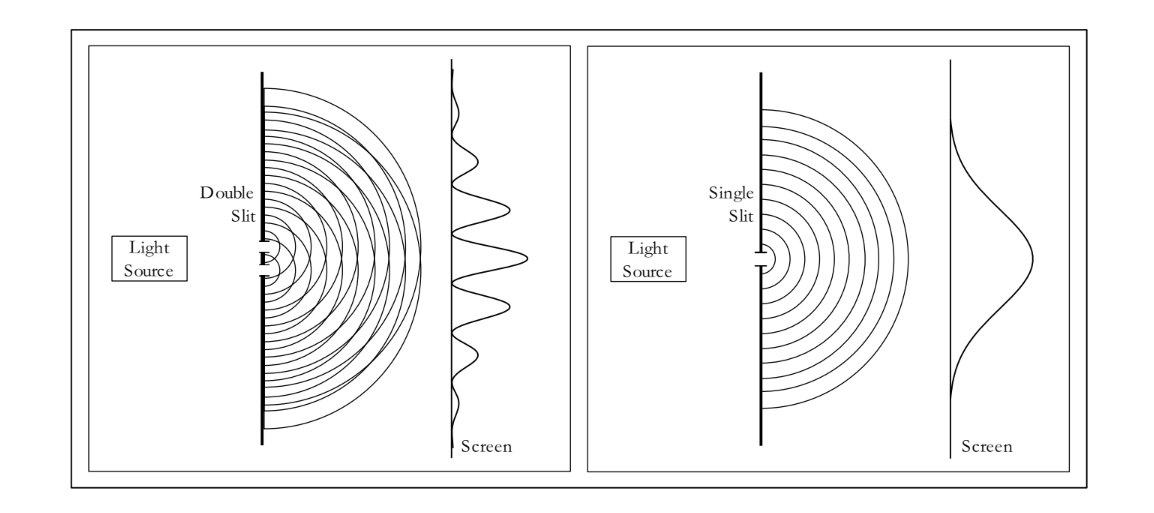
\includegraphics[width=1\linewidth]{Images/Doubleslit.png}
    \caption{Double slit and single-slit diffraction}
    \label{fig:slitexperiment}
\end{figure}

Next, we consider the situation for waves, for example water waves. A water wave doesn't go through either slit 1 or slit 2, it goes through both. you should imagine the rest of 1 water wave as it approaches the slit. As it hits the slit, the wave is blocked at all places but the two slits, and waves on the other side are generated at each slit as depicted in the figure \ref{fig:slitexperiment}.

When the new waves generated at each slit run into each other, interference occurs. We can see this by plotting the intensity (that is, the amount of energy carried by the waves) at each point y along the viewing screen. What we see is the familiar interference pattern seen in figure \ref{fig:slitexperiment}. The dark patches of the interference pattern seen in figure \ref{fig:slitexperiment} occur where the wave from the first slit arrives perfectly out of sync with wave from the second slit, while the bright points are where the two arrive in sync. For example, the bright spot right in the middle is bright because each wave travels the exact same distance from their respective slits to the screen, so they arrive in sync. The first dark spots are where the wave from one slit traveled exactly half of a wavelength longer than the other wave, thus they arrive at opposite points in their cycle and cancel. Here, it is not the intensities coming from each slit that add, but the height of the wave. This differs in the case of bullets: $I_{12}(y)\neq I_1(y)+I_2(y)$, but $h_{12}(y)=h_1(y)+h_2(y)$, and $I_{12}(y)=h(y)^2$, where $h9y)$ is the height of the wave and $I(y)$ is the intensity, or energy, of the wave.

Before we can say what light does, we need one more crucial piece of information. What happens when we turn down the intensity in both of these examples?

In the case of bullets, turning down the intensity means turning down the rate at which the bullets are fired. When we turn down the intensity, each time a bullet hits the screen it transfers the same amount of energy, but the frequency at which bullets hit the screen becomes less.

With water waves, turning down the intensity means making the wave amplitudes smaller. Each time a wave hits the screen it transfer less energy, but the frequency of the waves hitting the screen is unchanged.

Now what happens when we do this experiment with light. As Young observed in 1802, light makes an interference pattern on the screen. From this observation he concluded that the nature of light is wavelike, and reasonably so!.  However, Young was unable at the time to turn down the intensity of light to see the problem with the wave explanation.

Picture now that the observation screen is made of thousands of tiny little photo-detectors that can detect the energy they absorb. For high intensities the photo-detectors individually are picking up a lot of energy, and when we plot the intensity against the position y along the screen we see the same interference pattern as described earlier. Now, turn the intensity of the light very very low. At first, the intensity scales down lower and lower everywhere, just like a wave. But as soon as we get low enough, the energy that the photo-detectors report reaches a minimum energy, and all of the detectors are reporting the same energy, call it $E_0$, just at different rates. This energy corresponds to the energy carried by an individual photon, and at this stage we see what is called quantization of light. Photo-detectors that are in the bright spots of the interference pattern report the energy $E_0$ very frequently, while the darker areas report the energy $E_0$ at lower rates. Totally dark points still report nothing. This behavior is the behavior of bullets not waves! We now see that photons behave unlike either bullets or waves, but like something entirely different.

Turn down, the intensity so low that only one photo-detector reports something each second. in other words, the source only sends one photon at at time. Each time a detector receives a photon, we record where on the array it landed and plot it on a graph. The distribution we draw will reflect the probability that a single photon will land at a particular point.

Logically we think that the photon will either go through one slit or the other. Then, like the bullets, the probability that the photon lands at a point y should be $P_{12}(y)=P_1(y)+P_2(y)$ and the distribution we expect to see is the two peaked distribution of the bullets. But this is not what we see at all.

What we actually see is the same interference pattern as before! But how can this be? For there to be an interference pattern, light coming from one slit must interfere with light from the other slit; but there is only one photon going through at a time! The modern explanation is that the photon actually goes through both the slits at the same time, and interferes with itself. The mathematics is analogous to that in the case of water waves. We say that the probability $P(y)$ that a photon is detected at $y$ is proportional to the square of some quantity $a(y)$, which we call a probability amplitude. Now probability amplitudes for different alternatives add up. So $a_{12}(y)=a_{1}(y)+a_2(y)$. But $P_{12}(y)=|a_{12}(y)|^2\neq |a_1(y)|^2+|a_2(y)|^2=P_1(y)+P_2(y)$.

Logically, we can ask which slit the photon went through, and try to measure it. Thus, we might construct a double slit experiment where we put a photo-detector at each slit, so that each time a photon comes through the experiment we see which slit it went through and where it hits on the screen. but when such an experiment is performed, the interference pattern gets completely washed out! The very fact that we know which slit the photon goes through makes the interference pattern go away. This is the first example we see of how measuring a quantum system alters the system.

Here the photon looks both like a particle, a discreet package , and a wave that can have interference. It seems that the photon acts like both a wave and a particle, but at the same time it doesn't exactly behave like either. This is what is commonly known as the wave-particle duality, usually though of as a paradox. The resolutions is that the quantum mechanical behavior of matter is unique, something entirely new.

What may be more mind blowing still is that if we conduct the exact same experiment with electrons instead of light, we get the exact same results! Although it is common to imagine electrons as tiny little charged spheres, they are actually quantum entities, neither wave nor particle but understood by their wave function.

The truth is that there is no paradox, just an absence of intuition for quantum entities. Why should they be intuitive? Things on our scale do not behave like wave functions, and unless we conduct wild experiments like this we do not see the effects of quantum mechanics.
``  
\section{The Coin Experiment: Analogy for intuition}
Consider an unbiased coin, a preliminary high school knowledge will tell you that if you toss a coin the probability of getting heads or tails either is $1/2$. Given a coin we can either toss it or look at the coin. Note that we don't know the side of the coin facing up unless and until we look at the coin. This action of looking at the coin let us call it as measurement. Thus, given a coin we can perform two operations, either measurement or toss a coin i.e. we can either see the side facing up or toss the coin. Let us now move on to the mathematical framework. Consider that we don't know the state of the coin initially, so it can be either heads or tails with equal probability of $1/2$ and hence can be written as
\[
\begin{pmatrix} 1/2 \\ 1/2 \end{pmatrix}
\]
where the entry in the first row corresponds to the probability of seeing heads ($=1/2$) and the entry in the second row corresponds to seeing tails ($=1/2$) upon measurement. Note that the sum of the entries in the column must be equal to 1. Now we can either look at the coin i.e. do a measurement or toss a coin. Let us toss the coin. Now since it's an unbiased coin the state of the vector will not change even after tossing the coin. Mathematically, this can be represented by a linear operation i.e. matrix-vector multiplication operation where the matrix corresponds to the operation of tossing the coin. This is shown as follows:
\[
\begin{pmatrix} 1/2 & 1/2 \\ 1/2 & 1/2 \end{pmatrix} \begin{pmatrix} 1/2 \\ 1/2 \end{pmatrix} = \begin{pmatrix} 1/2 \\ 1/2 \end{pmatrix}
\]
where the matrix corresponds to the operation of tossing a coin and the vector is the state vector of the coin before tossing the coin. The state vector indicates that the probability of measuring heads is $1/2$ and probability measuring tails is $1/2$ upon measurement. Now if we perform a measurement i.e. look at the coin the probabilistic state of the coin it will either collapse to the following
\[
\begin{pmatrix} 1 \\ 0 \end{pmatrix} or \begin{pmatrix} 0 \\ 1 \end{pmatrix} 
\]
 for heads and tails respectively. Let us call this as basis states. Thus, if we perform another measurement the next time we will get Heads with certainty or tails with certainty depending upon the results of the previous measurement as indicated by the state vector which is also consistent with the real world results. Thus, we have a working mathematical framework of tossing a coin. Suppose, upon measurement we had found that the result of the state was head and hence the state vector was $\begin{pmatrix} 1 \\ 0 \end{pmatrix}$. Now when we toss the coin, we get
 \[
 \begin{pmatrix} 1/2 & 1/2 \\ 1/2 & 1/2 \end{pmatrix} \begin{pmatrix} 1 \\ 0 \end{pmatrix} = \begin{pmatrix} 1/2 \\ 1/2 \end{pmatrix}
 \]
 which is as we expected that now upon measurement the probability of getting heads is equal to the probability of getting tails $(=1/2)$. All the mathematical framework is consistent with the real world experiences. Now, no matter how many times we toss the coin the state of the vector will remain the same i.e. probability of getting heads is equal to the probability of getting tails $=1/2$ unless and until we perform a measurement by looking at the coin whereupon it collapses to one of the basis states.
Note that the state vector is also the eigen vector corresponding to the eigen value of 1 of the matrix (operation matrix of tossing the coin).

Let us make it more interesting by taking a biased coin. Let the probability of getting heads be 1/4 and of getting tails be 3/4. Thus the state vector corresponding to it will be
\[
\begin{pmatrix} 1/4 \\ 3/4 \end{pmatrix}
\]
We can now perform a measurement or toss the coin. Consider we don't know the state initially and we toss the coin, then the matrix-vector linear operation corresponding to the operation of tossing the coin and the state vector will be
\[
\begin{pmatrix} 1/4 & 1/4 \\ 3/4 & 3/4 \end{pmatrix}\begin{pmatrix} 1/4 \\ 3/4 \end{pmatrix} = \begin{pmatrix} 1/4 \\ 3/4 \end{pmatrix}
\]
Thus indicates that upon measurement we will get heads with a probability of $1/4$ and tails with a probability of $3/4$. No matter how many times we toss the coin the state of the vector will remain the same. Upon measurement the state will collapse to one of the basis states
\[
\begin{pmatrix} 1 \\ 0 \end{pmatrix} or \begin{pmatrix} 0 \\1 \end{pmatrix}
\]
Say upon measurement we found that it was Tails i.e. the state vector collapsed to $\begin{pmatrix} 0 \\1\end{pmatrix}$. Then again upon tossing the coin the state vector again be in a probabilistic state as follows:
\[
\begin{pmatrix} 1/4 & 1/4 \\3/4 & 3/4 \end{pmatrix} \begin{pmatrix} 0 \\ 1 \end{pmatrix} = \begin{pmatrix} 1/4 \\ 3/4\end{pmatrix}
\]
as expected. The state of the coin after tossing will again be a probabilistic state will the probability of getting heads being $1/4$ and the probability of tails being $3/4$ upon measurement.

Now, let us take this a step further. Note that we can write $\begin{pmatrix} 1/4 \\ 3/4 \end{pmatrix} = 1/4 \begin{pmatrix} 1 \\ 0 \end{pmatrix} + 3/4 \begin{pmatrix} 0 \\1\end{pmatrix}$. Note that we can write the state vector of the coin at any intermediate state as a linear combination of the basis state (since the basis states are two linearly independent orthogonal vectors, they span the entire 2D Vector space and hence any vector in the 2D space can be written as a linear combination of these two vectors). Thus, we can write the state vector of coin at any time as the linear combination of the basis states as shown below:
\[
\begin{pmatrix} \alpha \\ \beta \end{pmatrix} = \alpha \begin{pmatrix} 1 \\ 0 \end{pmatrix} + \beta \begin{pmatrix} 0 \\ 1 \end{pmatrix}
\]
for $\alpha, \beta \in \mathbb{R}$. Thus, the state vector of the coin always exists as a linear combination of the basis states. The operation of tossing the coin is simply a matrix-vector multiplication with the state as follows.
\begin{align*}
\begin{pmatrix} 1/4 & 1/4 \\3/4 & 3/4 \end{pmatrix} \begin{pmatrix} \alpha \\ \beta \end{pmatrix} &= \alpha \begin{pmatrix} 1/4 & 1/4 \\3/4 & 3/4 \end{pmatrix} \begin{pmatrix} 1 \\ 0 \end{pmatrix} + \beta \begin{pmatrix} 1/4 & 1/4 \\3/4 & 3/4 \end{pmatrix} \begin{pmatrix} 0 \\ 1 \end{pmatrix}\\
&= \alpha \begin{pmatrix} 1/4 \\ 3/4 \end{pmatrix} + \beta \begin{pmatrix} 1/4 \\ 3/4 \end{pmatrix}\\
&=(\alpha + \beta) \begin{pmatrix} 1/4 \\ 3/4 \end{pmatrix}
\end{align*}
Note that if we perform a measurement just after another measurement then the state of the vector remains unchanged i.e. say upon measurement we saw that the state vector was Heads then if we perform another measurement operation just after the first one (i.e. without tossing the coin) then the state vector will not change and will remain as Heads. No matter the amount of time you perform consecutive measurements the state vector once collapsed to either of the basis state in the first measurement remains the same throughout. But if we perform a matrix operation (coin toss) it will then again be in a probabilistic (or linear combination sometimes called a superposition) state.

In conclusion, we saw that the state vector is a linear combination of the basis vector (with real coefficients) and there are two categories of operations we can perform on the coin either measurement or toss a coin. Similar is the case with qubits. This linear combination of basis states is what sometimes referred to as the superposition principle.

For a qubit, the state vector is a linear combination (also called superposition) of the basis states (or vectors) (with complex coefficients) and there are two types of operations we can perform on qubits either measurement (in which case it collapses to one of the basis states) or a matrix multiplication (here the matrix is unitary as a result of Axiom of Quantum mechanics we will later see). Thus, we can define the basis vectors/states for the purpose of quantum computing as follows:
\[
\ket{0}=\begin{pmatrix} 1 \\ 0 \end{pmatrix}, \ket{1}=\begin{pmatrix} 0 \\ 1 \end{pmatrix}
\]
and thus the state vector of a qubit is given as
\[
\ket{v}=\begin{pmatrix} \alpha \\ \beta \end{pmatrix} = \alpha \begin{pmatrix} 1 \\ 0 \end{pmatrix} + \beta \begin{pmatrix} 0 \\ 1 \end{pmatrix}
\]
where $\alpha,\beta \in \mathbb{C}$. Thus, we can perform either of the two operations measurement or a matrix operation (manipulation of qubits). Upon measurement it will either collapse to either one of the basis states. The condition for manipulation of a matrix by a qubit is that it must be unitary. Thus, matrix multiplication will be as follows:
\[
Uv=\begin{pmatrix} a & b \\ c & d \end{pmatrix}\begin{pmatrix} \alpha \\ \beta \end{pmatrix} =\begin{pmatrix} a \alpha + b\beta \\ c\alpha + d\beta \end{pmatrix}
\]
where U is a unitary matrix ($U^{\dagger}U=UU^{\dagger}=I$).
There is another restriction that the norm of the state vector must be unit norm ($\|\ket{v}\|=1$). All these restrictions will be further explained in depth as part of axioms of Quantum Mechanics.

\section{Quantum Information}
We will look at Quantum information, a concept on which quantum computation is based.

\subsection{The Classical Information}
To describe quantum information and how it works, we will begin with an overview of classical information. Some readers may wonder why we choose to devote so much attention to classical information in a course on quantum information, but there are good reasons. For one, although quantum and classical information are different in some pretty spectacular ways, their mathematical descriptions are actually quite similar.

Classical information also serves as a familiar point of reference when studying quantum information, as well as a source of analogy that goes a surprisingly long way. It is common that people ask questions about quantum information that have natural classical analogs — often with simple answers that can provide both clarity and insight into the original questions about quantum information. Indeed, it is not at all unreasonable to claim that one cannot truly understand quantum information without understanding classical information.

Some readers may already be familiar with the material to be discussed in this section, while others may not — but the discussion is meant for both audiences. In addition to highlighting the aspects of classical information that are most relevant to an introduction to quantum information, this section introduces the Dirac notation, which is often used to describe vectors and matrices in quantum information and computation. As it turns out, the Dirac notation is not specific to quantum information: it can equally well be used in the context of classical information, as well as for many other settings in which vectors and matrices arise
\subsection{A probabilistic model}
Let us start classically, with a model that will probably seem completely simple to every one. Imagine that we have some physical device, called X, that has some finite, non-empty set $\Sigma$ of possible state (classical states). For example, we might have $\Sigma = \{0,1\}$, in which case we would think of X as representing a bit. For the following discussion let us restrict ourselves to this example (but keep in mind that everything can be generalized to sets other than $\{0,1\}$).

Suppose that we do not necessarily have complete information about the state of X, but instead represent our knowledge of its state by assigning probabilities to different states. For example, we might have
\[
Pr[\text{state of X is 0}]=1/4
\]
\[
Pr[\text{state of X is 1}]=3/4
\]
Mathematically we can represent this type of knowledge about the state X with a probability vector, which is a column vector whose entries are all non-negative real numbers that sum to 1. In the case at hand, the associated probability vector is
\[
v=\begin{pmatrix} 1/4 \\ 3/4 \end{pmatrix}
\]
The understanding is that the entries of $v$ are indexed by $\Sigma$, and when we write such a vector in the above form we are using the most natural way of ordering the elements of $\Sigma$.$1/4$ entry indexed by 0, $3/4$ entry indexed by 1.

We may write $v[0]$ and $v[1]$ to refer to the entries of $v$ when necessary.

What happens when you look at X? Of course you will not see a probability vector $v$. instead you will see some element of $\Sigma$. If our representation of the state of X by a probability vector $v$ is in some way meaningful, you may as well imagine that the state you saw was determined randomly according to the probabilities associated with various states. Notice that by looking at the sate of X you effectively change the description of your knowledge of its state. Continuing with the above example, if you look and see that the state is 0, the description of your knowledge changes from $v$ to a new probability vector $w$:
\[
v=\begin{pmatrix} 1/4 \\ 3/4 \end{pmatrix} \rightarrow w=\begin{pmatrix} 1 \\ 0 \end{pmatrix}
\]
You know that the state is 0, and the vector w represents this knowledge. If you saw the state was 1 instead of 0, the vector would become
\[
\begin{pmatrix} 0 \\ 1 \end{pmatrix}
\]
instead.

What sorts of operation can you imagine performing on X? There are not very many deterministic operations: you could initialize X to either 0 or 1, you could not perform a NOT operation to X, or you could do nothing to X (which can still be considered an operation even though it has no effect). You could also perform an operation involving randomness - for instance perform a NOT operation with probability $1/100$, and other wise do nothing. I claim that any physically meaningful operation can be represented by a matrix, with the effect of the operation being determined by the matrix-vector multiplication. For instance, these four matrices
\[
INIT_0 = \begin{pmatrix} 1 & 1 \\ 0 & 0\end{pmatrix}, INIT_1= \begin{pmatrix} 0 & 0 \\ 1 & 1 \end{pmatrix}, 
NOT = \begin{pmatrix} 0 & 1 \\ 1 & 0\end{pmatrix}, and \quad I = \begin{pmatrix} 1 & 0 \\ 0 & 1\end{pmatrix}
\]
represent the deterministic operators mentioned above. For example, if our knowledge of the state of X is represented by
\[
v=\begin{pmatrix}1/4 \\ 3/4 \end{pmatrix}
\]
and we perform a NOT operation on X, the new probability vector that results is
\[
w=\begin{pmatrix} 0 & 1 \\ 1 & 0 \end{pmatrix}\begin{pmatrix} 1/4 \\3/4 \end{pmatrix} =\begin{pmatrix}3/4 \ 1/4 \end{pmatrix}
\]
The probabilistic operation mentioned above is represented by the matrix
\[
\begin{pmatrix} \frac{99}{100} & \frac{1}{100} \\ \frac{1}{100} & \frac{99}{100} \end{pmatrix}
\]
All of these matrices have the property that (i) all entries are non-negative real numbers, and (ii) the entries of each column sum to 1. In other words, every column is a probability vector. Such matrices have a name: they are called stochastic matrices. in the simple model we are discussing, physically meaningful operations are described by stochastic matrices. it works the other way as well; any stochastic matrix describes some physically meaningful operation.

As mentioned before, this entire pictures is easily generalized to the case where $\Sigma$ is not necessarily $\{0,1\}$. In general the dimension of the vectors and matrices will be equal to the size of $\Sigma$.

\subsection{Quantum bits (qubits)}
The framework of quantum information works in a similar way to the simple probabilistic model we just saw, but with some key differences. Let us again imagine that we have a physical device called X. As before we imagine there is some set of $\Sigma$ of possible states of X, and we will again consider for now just the simple case $\Sigma=\{0,1\}$. At this point, to avoid confusion let us not refer to elements of $\Sigma$ as \textit{classical states}. Intuitively one can think of a classical state that you as a human can look at, touch and recognize without ambiguity. The device X will represent the quantum analogue of a bit, which we call a qubit.

We will represent out knowledge of X with column with column vectors indexed by $\Sigma$, but this time they will not be probability vectors. Instead of representing probability distributions, the vectors represent what we call a superposition or just a state (by which we mean a quantum state). For example, here are a few vectors representing superpositions:
\[
\begin{pmatrix} \frac{1}{\sqrt{2}} \\ -\frac{1}{\sqrt{2}} \end{pmatrix}, \begin{pmatrix} 1 \\ 0 \end{pmatrix}, \begin{pmatrix} \frac{3}{5} \\ \frac{4\iota}{5} \end{pmatrix}
\]

Notice that the entries in these vectors are not probabilities: they are not necessarily non-negative (in fact they are not even necessarily real numbers), and they do not necessarily sum to 1. We call these numbers amplitudes instead of probabilities. The condition that replaces probabilities summing to 1 in a probability vector is this: vectors representing superpositions have Eucledian length equal to 1. In the simple case at hand where $\Sigma = \{0,1\}$, this means that any vector representing a superposition has the form
\[
\begin{pmatrix} \alpha \\ \beta \end{pmatrix} 
\]
for $\alpha, \beta \in \mathbb{C}$ satisfying $|\alpha|^2+|\beta|^2=1$.

Similar to the probabilistic case, if you look at the qubit X you will not see a superposition. Instead you will see either 0 or 1 just like before. The probability associated with the two possible outcomes is given by the absolute value squared of the associated amplitude-so i the superposition of X is represented by the vector
\[
\begin{pmatrix} \alpha \\ \beta \end{pmatrix}
\]
any you look at X, you will see 0 with probability $|\alpha|^2$ and 1 with probability $|\beta|^2$. This is why we have the condition $|\alpha|^2+|\beta|^2$, because the probabilities have to sum to 1 for the model to make sense. The same rules apply as for the probabilities case for determining the superposition of X after you look at it: the superposition becomes
\[
\begin{pmatrix} 1 \\ 0 \end{pmatrix} or \begin{pmatrix} 0 \\1 \end{pmatrix}
\]
depending on whether you see 0 or 1, respectively.

So far the model does not seem qualitatively different from the probabilistic model, but that changes a lot when the possible operations that can be performed are considered. Again the possible operations are represented by matrices; but now instead of being stochastic matrices, the matrices that represent valid physical operations correspond to unitary matrices. A matrix is unitary if and only if it preserves the Eucledian norm. Fortunately there is a very simple condition to check this: a matrix U is unitary if and only if
\[
U^{\dagger}U=UU^{\dagger}=I
\]
where $U^{\dagger}$ is the conjugate transpose of U (meaning that you take the transpose of U and then take the complex conjugate of each of the entries). For example, these are unitary matrices:
\[
H=\begin{pmatrix} \frac{1}{\sqrt{2}} & \frac{1}{\sqrt{2}} \\ \frac{1}{\sqrt{2}} & -\frac{1}{\sqrt{2}} \end{pmatrix}, I=\begin{pmatrix} 1 & 0 \\0 & 1 \end{pmatrix}, NOT=\begin{pmatrix} 0 & 1 \\ 1 & 0\end{pmatrix}, R_{\theta} = \begin{pmatrix} \cos (\theta) & -\sin (\theta) \\ \sin(\theta) & \cos (\theta) \end{pmatrix}
\]
(for any real number $\theta$ in the case of $R_{\theta}$). For example, if X is a superposition described by
\[
v=\begin{pmatrix} 1 \\ 0 \end{pmatrix}
\]
and the operation corresponding to the matrix H (called the hadamard transform) is performed, the superposition becomes
\[
Hv=\begin{pmatrix} \frac{1}{\sqrt{2}} & \frac{1}{\sqrt{2}}\\\frac{1}{\sqrt{2}} & -\frac{1}{\sqrt{2}} \end{pmatrix}
\]
If you measured X at this point you would see outcome 0 or 1 with probability $1/2$. If you didn't measure and instead applied the Hadamard transform again, the superposition would become
\[
\begin{pmatrix} \frac{1}{\sqrt{2}} & \frac{1}{\sqrt{2}} \\ \frac{1}{\sqrt{2}} & -\frac{1}{\sqrt{2}} \end{pmatrix} = \begin{pmatrix} 1 \\ 0 \end{pmatrix}
\]
To recapitulate, these are the two things you can do to a qubit:
\begin{enumerate}
    \item \textbf{Perform a measurement.} If the superposition of the qubit is
    \[
    \begin{pmatrix} \alpha \\ \beta \end{pmatrix}
    \]
    and a measurement is performed, the outcomes is 0 or 1, with probabilities $|\alpha|^2$ and $|\beta|^2$, respectively. The superposition of the qubit becomes
    \[
    \begin{pmatrix} 1 \\ 0 \end{pmatrix}, \begin{pmatrix} 0 \\1 \end{pmatrix}
    \]
    depending on whether the measurement outcome was 0 or 1.
    \item \textbf{Perform a Unitary operation} For any unitary matrix U, the operation described by $U$ transforms any superposition $v$ into the superposition $Uv$.
\end{enumerate}

\begin{example}
    Suppose your friend has a qubit that he knows is in one of the two superpositions
    \[
    v_0=\begin{pmatrix} \frac{1}{\sqrt{2}} \\ \frac{1}{\sqrt{2}} \end{pmatrix} \text{ or } v_1=\begin{pmatrix} \frac{1}{\sqrt{2}} \\ -\frac{1}{\sqrt{2}} \end{pmatrix}
    \]
    but he isn't sure which. How can you help him determine which one it is?
    Measuring right away will not help - you would see a random bit 0 or 1 with equal probability in either case. instead,you should perform a Hadamard transform and them measure. Performing the hadamard transform changes the superposition as follows:
    \[
    Hv_0=\begin{pmatrix} 1 \\ 0\end{pmatrix} \quad \text{and} \quad Hv_1 =\begin{pmatrix} 0 \\1 \end{pmatrix}
    \]
    Now if you measure, you will see 0 (with certainty, meaning probability 1) if the original superposition was $v_0$ and you will see 1 (with certainty) if the original superposition was $v_1$.
\end{example}

Thus instead of being just 0 and 1, quantum bits can be in a superposition between 0 and 1. Since "quantum bit" is somewhat long, researchers simply use the term "qubit" to refer to a quantum bit. Thinking of bit as vectors, a qubit can be described by a vector $\ket{v} \in \mathbb{C}^2$. the vector space $\mathbb{C}^2$. The vector space $\mathbb{C}^2$ is also known as the state space of the qubit. An example of qubit state is
\[
\ket{+}=\frac{1}{\sqrt{2}}(\ket{0}+\ket{1})
\]
It turns out that in order to be a valid qubit, $\ket{v}$ must be normalized, just as the vectors $\ket{0}$ and $\ket{1}$ corresponding to classical bits were indeed normalized. For the moment, let us just take this as a rule leading to the following definition.

\begin{definition}
    \textbf{Qubit} A (pure) state of a qubit can be represented as a 2-dimensional ket vector $\ket{\psi} \in \mathbb{C}^2$.
    \[
    \ket{\psi}=\alpha\ket{0}+\beta\ket{1}, \quad \text{where $\alpha,\beta \in \mathbb{C}$ and $|\alpha|^2+|\beta|^2=1$}
    \]
    The condition on $\alpha$ and $\beta$ means that $\ket{\psi}$ is normalized. These complex numbers $\alpha$ and $\beta$ are also called amplitudes of $\ket{\psi}$.
\end{definition}

Throughout these lectures we will be mostly focusing on encoding information in qubits. However in general, quantum information can also be encoded in higher dimensional quantum systems. Therefore, one can similarly define a qudit as below:
\begin{definition}
    A qudit, or a d-dimensional quantum system can be represented as a d-dimensional ket vector $\ket{\psi} \in \mathbb{C}^d$
    \[
    \ket{\psi}=\sum_{i=0}^{d-1} \alpha_i\ket{i}, \quad \text{where $\forall i, \alpha_i \in \mathbb{C}$ and $\sum_{i=0}^{d-1} |\alpha_i|^2=1$ }
    \]
    The condition on the coefficients $\alpha_i$ means that $\ket{\psi}$ is a vector of length of 1.
\end{definition}
\begin{example}
    An example of a qubit is given by the vector $\ket{-}=\frac{1}{\sqrt{2}}(\ket{0}-\ket{1})$. The length of $\ket{-}$ is
    \[
    \braket{-|-}=\sqrt{\frac{1}{2}\begin{pmatrix} 1 & -1 \end{pmatrix} \begin{pmatrix} 1 \\ -1 \end{pmatrix}}=\sqrt{\frac{1}{2}2}=1
    \]
    So $\ket{-}$ is normalized.
\end{example}
\begin{example}
    Verify that for all values of $\theta$, $\ket{\psi}=\cos (\theta) \ket{0} + \sin (\theta) \ket{1}$ is a valid qubit state.
    \[
    |\cos (\theta)|^2+|\sin (\theta)|^2=\cos^2 (\theta) + \sin^2 (\theta)=1
    \]
    Thus, clearly it is normalized for all values of $\theta$.
\end{example}
In our definition of qubits, we started from a way to write classical bits as vectors $\ket{0}$ and $\ket{1}$. Note that these two vectors are orthonormal, which in the quantum notation can be expressed as $\braket{1|0}=0$ and $\braket{1|1}=\braket{0|0}=1$. These two vectors thus form a basis for $\mathbb{C}^2$, in that any vector $\ket{v}\in \mathbb{C}^2$ can be written as $\ket{v}=\alpha \ket{0} +\beta \ket{1}$ for some coefficients $\alpha,\beta \in \mathbb{C}$. This basis corresponding to "classical" bits is used so often that it carries a special name:

\begin{enumerate}
    \item \begin{definition}
        \textbf{Computational Basis/Standard Basis:} Consider the 2-dimensional complex vector space $\mathbb{C}^2$. The standard basis, or sometimes known as the computational basis, $\mathcal{S}=\{\ket{0},\ket{1}\}$ is an orthonormal basis for this vector space, where the basis vectors are
        \[
        \ket{0}=\begin{pmatrix} 1 \\ 0 \end{pmatrix}, \ket{1}=\begin{pmatrix} 0 \\ 1 \end{pmatrix}
        \]
        In general, for a d-dimensional complex vector space $\mathbb{C}^d$. The standard basis or computational basis states are represented as $\ket{0},\ket{1},\ldots,\ket{d-1}$ where
        \[
        \ket{i}=\begin{pmatrix} \vdots \\ 0 \\ 1 \\ 0 \\ \vdots \\ \end{pmatrix}
        \]
        where it is a column vector of size $2^d \times 1$ with 1 at the ith location and 0 elsewhere.
    \end{definition}
Of course, there might be many other bases for $\mathbb{C}^2$. But here,we will discuss only those basis which are most frequently used.
    \item \begin{definition}\textbf{Hadamard Basis:} The Hadamard basis is an orthonormal basis in which the states are represented as $\mathcal{H}=\ket{+},\ket{-}$ where 
    \[\ket{+}=\dfrac{\ket{0}+\ket{1}}{\sqrt{2}}=\frac{1}{\sqrt{2}}\begin{pmatrix} 1 \\ 1 \end{pmatrix} \quad \text{and} \quad \ket{-}=\dfrac{\ket{0}-\ket{1}}{\sqrt{2}}=\frac{1}{\sqrt{2}}\begin{pmatrix} 1 \\-1\end{pmatrix}.
    \]
    \end{definition}
    \item \textbf{Y Basis:} The basis in which the states are represented as $\ket{+i},\ket{-i}$ where 
    \[\ket{+i}=\dfrac{\ket{0}+\iota\ket{1}}{\sqrt{2}}=\frac{1}{\sqrt{2}}\begin{pmatrix} 1 \\ \iota \end{pmatrix} \quad \text{and} \quad \ket{-i}=\dfrac{\ket{0}-\iota\ket{1}}{\sqrt{2}}=\frac{1}{\sqrt{2}}\begin{pmatrix} 1 \\ -\iota \end{pmatrix}
    \]
\end{enumerate}

\begin{example}
    We now verify that the hadamard basis is indeed orthonormal using the bra-ket notation as shown below:
    \[
    \braket{+|+}=\frac{1}{2} \begin{pmatrix} 1 & 1 \end{pmatrix} \begin{pmatrix} 1 \\ 1 \end{pmatrix} =\frac{1}{2}2=1\implies \sqrt{\braket{+|+}}=1
    \]
    So $\ket{+}$ is normalized. Furthermore, the inner product
    \[
    \braket{+|-}=\frac{1}{2}\begin{pmatrix} 1 & 1 \end{pmatrix} \begin{pmatrix} 1 \\ -1 \end{pmatrix} = 0
    \]
    So $\ket{+}$ and $\ket{-}$ are orthogonal to each other.
\end{example}

\begin{example}
    Express $\ket{1}$ in the Hadamard basis. That is, find coefficients $\alpha$ and $\beta$ such that $\ket{1}=\alpha\ket{+}+\beta\ket{-}$.
    Clearly, putting $\alpha=\frac{1}{\sqrt{2}}$ and $\beta=\frac{1}{\sqrt{2}}$ satisfies the system of linear equations.
\end{example}

The linear superposition $\ket{\psi}=\alpha\ket{0}+\beta \ket{1}$ is part of the private world of electron. For us to know the electron's state, we must make a measurement. making a measurement gives us a single classical bit of information 0 or 1. The simplest measurement is in the standard basis, and measuring $\ket{\psi}$ in this $\{\ket{0},\ket{1}\}$ basis yields 0 with probability $|\alpha|^2$, and 1 with probability $|\beta|^2$,.

One important aspect of the measurement process is that it alters the state of the qubit: the effect of the measurement is that the new state is exactly the outcome of the measurement. i.e., if the outcome of the measurement of $\ket{\psi}=\alpha \ket{0}+\beta\ket{1}$ yields 0, then following the measurement, the qubit is in the state $\ket{0}$. This implies that you cannot collect any additional information about $\alpha,\beta$ by repeating the measurement.

More generally, we may choose any orthogonal basis $\{\ket{v},\ket{w}\}$ and measure the qubit in that basis. To do this, we rewrite our state in that basis: $\ket{\psi}=\alpha'\ket{v}+\beta'\ket{w}$. The outcome is $v$ with probability $|\alpha'|^2$, and $\ket{w}$ with probability $|\beta'|^2$. If the outcome of the measurement on $\ket{\psi}$ yields $\ket{v}$, then as before, the qubit is then in state $\ket{v}$.

\subsection{Example of Qubits}
\subsubsection{Atomic Orbitals}
The electrons within an atom exist in quantized energy levels. Qualitatively these electronic orbits (or "orbitals" as we like to call them) can be thought of as resonating standing waves, in close analogy to the vibrating waves one observes on a tightly held piece of string. Two such levels can be isolated to configure the basis states for a qubit.

\subsubsection{Photon Polarization}
Classically, a photon may be described as a traveling electromagnetic wave. This description can be fleshed out using Maxwell's equation, but for out purposes we will focus simply on the fact that an electromagnetic wave has a polarization which describes the orientation of the electric field oscillations (see figure). So, for a given direction of photon motion, the photon's polarization axis might lie anywhere in a 2-d plane perpendicular to that motion. It is thus natural to pick an orthonormal 2-d basis (such as $\vec{x}$ and $\vec{y}$, or "vertical" and "horizontal") to describe the polarization state (i.e. polarization direction) of a photon. In a quantum mechanical description, this 2-d nature of the photon polarization is represented by a qubit, where the amplitude of the overall polarization state in each basis vector is just the projection of the polarization in that direction.

The polarization of a photon can be measured by using a polaroid film or a calcite crystal. A suitably oriented sheet transmits x-polarized photons and absorbs y-polarized photons. Thus a photon that is in a superposition $\ket{\phi}=\alpha\ket{x}+\beta \ket{y}$ is transmitted with probability $|\alpha|^2$. If the photon now encounters another polaroid sheet with the same orientation, then it is transmitted with probability 1. On the other hand, if the second polaroid sheet has its axes crossed at right angles to the first one, then if the photon is transmitted by the first polaroid, then it is definitely absorbed by the second sheet. This pair of polarized sheets at right angles thus blocks all the light. A somewhat counter-intuitive result is not obtained by interposing a third polaroid sheet at a 45 degree angle between the first two. Now a photon that is transmitted by the first sheet makes it through the next two with some non zero probability.

To see this first observe that any photon transmitted through the first filter is in the state, $\ket{0}$. The probability this photon is transmitted through the second filter is $1/2$ since it is exactly the probability that a qubit in the state $\ket{0}$ ends up in the state $\ket{+}$ when measured in the $\ket{+},\ket{-}$ basis. We can repeat this reasoning for the third filer, except now we have a qubit in state $\ket{+}$ being measured in the $\ket{0},\ket{1}$ basis - the change that the outcome is $\ket{0}$ is once again $1/2$.

\subsubsection{Spins}
Like photon polarization, the spin of a (spin-1/2) particle is a two-state system, and can be described by a qubit.Very roughly speaking, the spin is a quantum description of the magnetic moemnt of an electron which behaves like a spinning charge. The two allowed states can roughly be thought of as clockwise rotations ("spin-up") and counter clockwise rotations ("spin-down").

\subsection{Multiple Qubits}
In order to talk about what happens when we have multiple qubits, it will be helpful to briefly return to the probabilistic model from before. Suppose that X and Y are devices that implement bits. Then there are 4 possible states of the pair (X,Y), namely 00, 01, 10 and 11. Thus, our set of states $\Sigma$ corresponding to this pair is now $\{00,01,10,11\}$. In the probabilistic model we represent our knowledge of the state of the pair (X,Y) with a 4 dimensional probability vector. For example we could have the following probability vector
\[
\begin{pmatrix} \frac{1}{8} \\ \frac{1}{2} \\ 0 \\ \frac{3}{8} \end{pmatrix}
\]
with the first entry indicating the probability associated with state 00, second entry denoting the probability associated with state 01, third entry denoting the probability associated with state 10, fourth entry denoting the probability associated with state 11. (The vector indices are labelled by the states in the order given by binary notation.) Operations again correspond to stochastic matrices, but this time the matrices are $4 \times 4$ matrices. For example, the matrix
\[
\begin{pmatrix} 1 & 0 & 0 & 0 \\ 0 & 1 & 0 & 0 \\ 0 & 0 & \frac{1}{2} & \frac{1}{2} \\ 0 & 0 & \frac{1}{2} & \frac{1}{2} \end{pmatrix}
\]
is stochastic. It happens to correspond to the operation where you do nothing if the first bit is 0 but if the first bit is 1 then replace the second bit with a random bit.

The quantum variant works in an analogous way. If we have two qubits (X,Y), then a superposition of these two qubits is a 4-dimensional vector with Eucledian length equal to 1. For example:
\[
\begin{pmatrix} \frac{1}{\sqrt{2}} \\ 0 \\ \frac{\iota}{2} \\ -\frac{1}{2} \end{pmatrix}
\]
Measurement works the same way as before, except that the outcome will be two bits. For example, measuring the previous superposition gives results as follows:
\[
\text{00 with probability} |\frac{1}{\sqrt{2}}|^2=\frac{1}{2}
\]
\[
\text{01 with probability} |0|^2=0
\]
\[
\text{10 with probability} |\frac{\iota}{2}|^2=\frac{1}{4}
\]
\[
\text{11 with probability} |=\frac{1}{2}|^2=\frac{1}{4}
\]
We can also measure only one qubit out of the two bits leaving the other alone, which is called partial measurement. We will later on see what happens in case of partial measurement. Unitary operations also work the same way as before, but this time are $4 \times 4$ matrices. For example, there is a 2 qubit unitary operation called controlled-NOT:
\[
\begin{pmatrix} 1 & 0 & 0 & 0 \\ 0 & 1 & 0 & 0 \\ 0 & 0 & 0 & 1\\ 0 & 0 & 1 & 0 \end{pmatrix}
\]
The same pattern is used for 3 qubits, 4 qubits etc. The dimension of the vectors and matrices grows exponentially: 8 dimensional vectors for 3 qubits, 16 dimensional vectors for 4 qubits, etc.

By the way there is no reason you cannot consider the model for any other choice of $\Sigma$, instead of $\Sigma$ corresponding to all possible strings of a given length. Typically, however, we will focus on the case where $\Sigma=\{0,1\}^n$ for positive integer n.

Classically, if we have two bits, we write them as '00','01',10','11'. But how can we write two qubits? One strategy is to again associate each of them two classical bits $x_1,x_2 \in \{0,1\}^2$ with a vector. labeling the first qubit A and the second one B, we could perform the mapping from strings to orthonormal vectors as
\[
0_A0_B\rightarrow \ket{00}_{AB}=\begin{pmatrix} 1 \\0 \\0 \\ 0 \end{pmatrix} \quad 0_A1_B\rightarrow \ket{01}_{AB}=\begin{pmatrix} 0 \\ 1 \\ 0 \\ 0 \end{pmatrix}
\]
\[
1_A0_B\rightarrow \ket{10}_{AB}=\begin{pmatrix} 0 \\ 0 \\ 1 \\0 \end{pmatrix} \quad 1_A1_B\rightarrow \ket{11}_{AB}=\begin{pmatrix} 0 \\ 0 \\ 0 \\ 1 \end{pmatrix}
\]
Note that the resulting vectors are in $\mathbb{C}^4$ with dimension $d=2^2=4$, where the dimension corresponds to the number of possible strings. It turns out that one can write a two-qubit state $\ket{\psi}_{AB}\in\mathbb{C}^4$ as a superposition of these vectors, where we again demand that $\ket{\psi}_{AB}$ is normalized. As an example, let us consider a state $\ket{\psi}_{AB}$ that is an equal superposition fo all above standard basis vectors:
\begin{align*}
\ket{\psi}_{AB}&=\frac{1}{2}\ket{00}_{AB}+\frac{1}{2}\ket{01}_{AB}+\frac{1}{2}\ket{10}_{AB}+\frac{1}{2}\ket{11}_{AB}\\
&=\frac{1}{2}\begin{pmatrix} 1 \\ 0 \\ 0 \\ 0 \end{pmatrix}+\frac{1}{2}\begin{pmatrix} 0 \\ 1 \\ 0 \\ 0 \end{pmatrix} + \frac{1}{2}\begin{pmatrix} 0 \\ 0 \\ 1 \\ 0 \end{pmatrix} + \frac{1}{2}\begin{pmatrix} 0 \\ 0 \\ 0 \\ 1 \end{pmatrix}\\
&=\frac{1}{2}\begin{pmatrix} 1 \\ 1 \\ 1 \\ 1 \end{pmatrix}
\end{align*}
The sum of amplitudes $\frac{1}{2}$ squared is $4\frac{1}{2^2}=1$, therefore $\ket{\psi}$ is a valid two qubit quantum state. As you might have guessed, we now proceed analogously when considering n qubits. To address
multiple qubits, we first look at the vector representation for multiple classical bits. For binary
strings of length $n$, consider the vector space $\mathbb{C}^n$, where each coordinate is labeled by a string
$x = x_1,..., x_n$. There are a total of $d = 2^n$ such strings, so we can label each string $x$ with a different
integer $i \in [1,d]$. We can then express the string $x$ as a vector $\ket{x_i}$ that is $0$ everywhere, except at the position labeled by $i$. A quantum state of $n$ qubits can then be written as
\[
\ket{\psi}=\sum_{x\in\{0,1\}^n} \alpha_x\ket{x}
\]
with $\alpha_x\in\mathbb{C}$ and $\sum_x |\alpha_x|^2=1$. The numbers $\alpha_x$ are again called amplitudes. We emphasize that the dimension of the vector space $\mathbb{C}^{2^n}$ increases exponentially with the number $n$ of bits. The space $\mathbb{C}^d$ with $d=2^n$ is thereby called the state space of n qubits. This means that we need an exponential number of parameters $\alpha_x$ to keep track of only n qubits, in sharp contrast to the $n$ parameters $x_1,\ldots , x_n$ to describe $n$ classical bits. You might wonder whether this was the only way to write down qubits. After all, we had simply chosen some mapping from strings of length $n$ to vectors in $\mathbb{C}^d$. Could we have chosen any other mapping from strings to vectors? It turns out that the answer to this is yes - as long as each string gets mapped to a vector that is orthonormal to the others. The mapping above, however, is very convenient and generally adopted within the realm of quantum computing. Analogous
to the case of a single qubit, the basis given by the set of vectors ${\ket{x} | x \in \{0,1\}^n}$ is called the
\textit{standard/computational basis}.

\begin{definition}
    \textbf{Standard basis for n qubits}. Consider the state space of n qubits $\mathbb{C}^d$. where $d=2^n$. For each distinct string $x \in \{0,1\}^n$. associate $x$ with a distinct integer $i \in \{1,2,\ldots ,d\}$. The standard basis for $\mathbb{C}^d$ is an orthonormal basis given by $\mathcal{S}_n=\{\ket{x} | x \in \{0,1\}^n$
    where $\ket{x}$ are d-dimensional vectors.
    \[
    \ket{x}=\begin{pmatrix} 0 \\ \vdots \\  1 \\ \vdots \\ 0 \end{pmatrix}
    \]
    where 1 is at the ith position.
\end{definition}
Let us summarize our discussion in the following definition of an n qubit quantum state.
\begin{definition}
    An n-qubit state $\ket{\psi} \in \mathbb{C}^d$ with $d=2^n$ can be written as a superposition of standard basis elements.
    \[
    \ket{\psi} = \sum_{x\in\{0,1\}^n}\alpha_x\ket{x}, \quad \text{where $\forall x, \alpha_x \in \mathbb{C}$ and $\sum_{x \in \{0,1\}^n} |\alpha_x|^2=1$}
    \]
\end{definition}
Let us now consider two examples of two qubit states. The first is so famous it carries a special
name and we will see it very frequently in the course of these notes.
\begin{example}
    Example 0.2.2 Consider two qubits A and B, in the two qubit state known as the EPR (Einstein, Podolsky and Rosen) pair, one can label the join state as AB
    \[
    \ket{EPR}_{AB}=\frac{1}{\sqrt{2}}(\ket{00}_{AB}+\ket{11}_{AB})=\frac{1}{\sqrt{2}}\begin{pmatrix} 1 \\ 0 \\ 0 \\ 0 \end{pmatrix} + \frac{1}{2}\begin{pmatrix} 0 \\ 0 \\ 0 \\ 1 \end{pmatrix}=\frac{1}{\sqrt{2}}\begin{pmatrix} 1 \\ 0 \\ 0 \\ 1 \end{pmatrix}
    \]
    which is an equal superposition between the vectors $\ket{00}_{AB}$ and $\ket{11}$. The length of this vector is given by the (square root o) inner product
    \begin{align*}
    \braket{EPR|EPR}_{AB}&=\frac{1}{\sqrt{2}}(\bra{00}_{AB}+\bra{11}_{AB})\cdot \frac{1}{\sqrt{2}}(\ket{00}_{AB}+\ket{11}_{AB})\\
    &=\frac{1}{2}(\braket{00|00}_{AB}+\braket{00|11}_{AB}+\braket{11|00}_{AB}+\braket{11|11}_{AB})\\
    &=\frac{1}{2}\cdot 2=1 \implies \sqrt{\braket{EPR|EPR}}=1
    \end{align*}
\end{example}
\begin{example}
    Consider the two qubit state
    \[
    \ket{\psi}_{AB}=\frac{1}{\sqrt{2}}(\ket{01}_{AB}+\ket{11}_{AB}\frac{1}{\sqrt{2}}\begin{pmatrix} 1\\ 0 \\ 0 \\ 1 \end{pmatrix}
    \]
    For this state, the second qubit always corresponds to bit 1. We will later see that this is significantly different state compared to $\ket{EPR}_{AB}$. It is not entangled!!.
\end{example}

\subsubsection{Tensor Products: How to combine qubits}

Returning again briefly to the probabilistic model, let us suppose that as before X and Y are devices
implementing bits, and the two devices are completely uncorrelated with one another—let us say
that the probability vector corresponding to X is
\[
v=\begin{pmatrix} \frac{2}{3} \\ \frac{1}{3} \end{pmatrix}
\]
and the probability vector corresponding to Y is
\[
w=\begin{pmatrix} \frac{1}{4} \\ \frac{3}{4} \end{pmatrix}
\]
Then the 4 dimensional probability vector corresponding to the pair (X, Y) is easily determined by
multiplying the corresponding probabilities. In particular, the resulting vector is
\[
v\otimes w= \begin{pmatrix} \frac{1}{6} \\ \frac{1}{2} \\ \frac{1}{12} \\ \frac{1}{4} \end{pmatrix}
\]
The operation $\otimes$ is called the Kronecker product or the tensor product. (It is most common in
quantum computing to use the term tensor product to refer to this operation.) In general, for any
two matrices
\[
A=\begin{pmatrix} a_{11} & a_{12} &\ldots & a_{1m} \\ a_{21} & a_{22} &\ldots &a_{2m} \\ \vdots & \vdots &\ddots & \vdots \\ a_{n1} & a_{n2} &\ldots & a_{nm} \end{pmatrix} \quad \text{and} \quad B=\begin{pmatrix} b_{11} & b_{12} &\ldots & b_{1l} \\ b_{21}& b_{22} & \ldots & b_{2l} \\ \vdots & \vdots & \ddots & \vdots \\ b_{k1} & b_{k2} & \ldots & b_{kl} \end{pmatrix}
\]
we define $A\otimes B$ to be the $nk \times ml$ matrix
\[
A\otimes B=\begin{pmatrix} a_{11}B & a_{12}B &\ldots & a_{1m}B \\ a_{21}B & a_{22}B &\ldots &a_{2m}B \\ \vdots & \vdots &\ddots & \vdots \\ a_{n1} B& a_{n2}B &\ldots & a_{nm}B \end{pmatrix}
\]
The definition works for vectors by thinking of them as matrices with only one column.
The tensor product satisfies many nice properties. For example, it is an associative operation;
$$(A \otimes B) \otimes  C = A \otimes (B \otimes C)$$ for any choice of matrices A, B and C. Thus, it makes sense to talk about products such as $A \otimes B \otimes C \otimes \ldots \otimes Z$ without including parentheses, because it doesn’t matter in which order the products are evaluated. Next, we have
\[
(A\otimes B)(C\otimes D)=(AC)\otimes (BD)
\]
for any choice of matrices A, B, C and D (assuming the sizes of the matrices are such that the
products AC and BD make sense). The distributive law holds for tensor products;
\[
A\otimes (B+C)=A\otimes B+A\otimes C \quad \text{and} \quad (A+B)\otimes C=A\otimes C+B\otimes C
\]
Also, for matrices A and B and any scalar $\alpha$, we have
\[
(\alpha A)\otimes B=A \otimes (\alpha B)=\alpha(A\otimes B)
\]
In other words, scalars “float freely” through the tensor product. A word of warning, however, is
that the tensor product is not commutative; in general it may be the case that $A\otimes B\neq B\otimes A$.

Not every probability vector v representing a distribution of (X, Y) can be written as a tensor
product. For example,
\[
v=\begin{pmatrix}1/2\\0\\0 \\ 1/2 \end{pmatrix}
\]
cannot be written as a tensor product. In this distribution we have
\[
Pr[\text{state of $(X,Y)$ is $00$}]=Pr[\text{state of $(X,Y)$ is }11]=\frac{1}{2}
\]
We say that X and Y are correlated in this case. The only way a probability vector can be written
as a tensor product is when the associated systems are uncorrelated (or independent).
As you might have guessed, we do exactly the same thing in the quantum case as in the classical, probabilistic case. If X and Y are qubits having associated superpositions
\[
v=\begin{pmatrix} \alpha \\ \beta \end{pmatrix} \quad \text{and} \quad w=\begin{pmatrix} \gamma \\ \delta \end{pmatrix}
\]
then the superposition of the pair (X, Y) is
\[
v\otimes w=\begin{pmatrix} \alpha\gamma \\ \alpha\delta \\ \beta\gamma\\\beta\delta \end{pmatrix}
\]
The superposition
\[
\begin{pmatrix} \frac{1}{\sqrt{2}} \\ 0 \\ 0 \\ \frac{1}{\sqrt{2}} \end{pmatrix}
\]
is an example of a superposition that cannot be written as a tensor product. In the quantum case,
this type of correlation between X and Y is special and we call it entanglement. We will talk about
entanglement a lot during the course.

For example, $\ket{1010}$ is a 16 dimensional vector with a 1 in the position indexed by $1010$ in binary (which is the eleventh entry because we start with 0000). The vector
\[
\frac{1}{\sqrt{2}} \ket{000000} +\frac{1}{\sqrt{2}}\ket{111111}
\]
would be written
\[
\begin{pmatrix} \frac{1}{\sqrt{2}} \\ 0 \\ \vdots \\ 0 \\\frac{1}{\sqrt{2}} \end{pmatrix}
\]
in the usual vector notation. An arbitrary vector with entries indexed by $\{0,1\}^n$, which perhaps refers to a superposition of n qubits, can again be written as a linear combination of the elements in the basis
\[
\{\ket{x}:x \in \{0,1\}^n\}
\]
for instance as
\[
\ket{\phi}=\sum_{x\in\{0,1\}^n} \alpha_x \ket{x}
\]

\begin{example}
    Let us suppose that we have two qubits X and Y in the superposition
    \[
    \begin{pmatrix} \frac{1}{\sqrt{2}} \\ 0 \\ 0 \\ \frac{1}{\sqrt{2}} \end{pmatrix}
    \]
    Using the Dirac notation we write this superposition as
    \[
    \frac{1}{\sqrt{2}}\ket{00}+\frac{1}{\sqrt{2}}\ket{11}
    \]
\end{example}

For every ket $\ket{\psi}$ there is a corresponding object $\bra{\psi}$, called a “bra”. You may think that this is
a strange name for a mathematical object, but the names “bra” and “ket” are derived from the the fact that when you put a bra and a ket together, you get a “bracket”. For this to make sense you
need to know what a bra is—for any vector $\ket{\psi}$ we define
\[
\bra{\psi}=(\ket{\psi})^{\dagger}
\]
which is the conjugate transpose of $\ket{\psi}$. In other words, $\bra{\psi}$ is the row vector you get by transposing
$\ket{\psi}$ and taking the conjugate of each of its entries. For instance:
\[
\ket{\psi}=\begin{pmatrix} \frac{1 + \iota }{2} \\ \frac{1}{\sqrt{2}} \end{pmatrix} \implies \bra{\psi}=\begin{pmatrix} \frac{1-\iota}{2} & \frac{1}{\sqrt{2}} \end{pmatrix}
\]
Now, when you juxtapose a bra and a ket, the implicit operation is matrix multiplication (thinking
of the vectors as matrices with only one row or one column). A row vector times a column vector
results in a scalar, and this scalar will be the inner product (or bracket) of the vectors involved. For
instance, if
\[
\ket{\psi}=\begin{pmatrix} \alpha \\ \beta \end{pmatrix} \quad \text{and}\quad \ket{\phi}=\begin{pmatrix} \gamma \\ \delta \end{pmatrix}
\]
then
\[
\braket{\psi|\phi} = \bra{\psi} \ket{\phi}=\begin{pmatrix} \overline{\alpha} & \overline{\beta} \end{pmatrix} \begin{pmatrix} \gamma \\ \delta \end{pmatrix} =\overline{\alpha}\gamma + \overline{\beta}\delta 
\]
When you have an expression such as
\[
\ket{\psi}=\sum_{x\in\{0,1\}^n} \alpha_x \ket{x}
\]
It is easy to express $\bra{\psi}$ using similar notation; it is
\[
\bra{\psi}=\sum_{x\in\{0,1\}^n} \overline{\alpha_x} \ket{x}
\]
When you juxtapose a ket and a bra in the opposite order, such as
\[
\ket{\psi}\bra{\phi}
\]
you do not get a scalar—a column vector times a row vector gives you a matrix. It is easy to
determine the action of this matrix on another vector. For instance,
\[
\ket{\psi}\bra{\phi}\ket{\gamma}=\ket{\psi}\braket{\phi|\gamma}=\braket{\phi|\gamma}\ket{\psi}
\]
Later on when we wish to speak at a higher level of abstraction about computational problems,
algorithms, etc., we may refer to |xi where x is some arbitrary mathematical object (such as a
matrix, a graph, or a list of numbers). In this case the interpretation is that we are implicitly
referring to the encoding of x with respect to some agreed upon encoding scheme.


Let’s imagine that we have two qubits, A and B. We know that we can describe the state of A
as $\ket{\psi}_A$and the one of B as $\ket{\phi}_B$. How can we write down the combined state $\ket{\psi}_{AB}$ of A and B together? The rule for computing the joint state is given by the so-called tensor product (sometimes also called Kronecker product). For two qubits
\[
\ket{\psi}_A=\alpha_A\ket{0}_A+\beta_A\ket{1}_A=\begin{pmatrix} \alpha_A \\ \beta_A \end{pmatrix}
\]
\[
\ket{\phi}_B=\alpha_B\ket{0}_B+\beta_B\ket{1}_B = \begin{pmatrix} \alpha_B \\ \beta_B\end{pmatrix}
\]
the joint state $\ket{\psi}_{AB} \in \mathbb{C}^2 \otimes \mathbb{C}^2$ can be expressed as the tensor product of individual vectors $\ket{\psi}_A$ and $\ket{\phi}_B$
\[
\ket{\psi}_{AB}=\ket{\psi}_A \otimes \ket{\phi}_B = \begin{pmatrix} \alpha_A \\ \beta_A \end{pmatrix} \otimes \ket{\psi}_B = \begin{pmatrix} \alpha_A \ket{\psi}_B \\ \beta_A\ket{\psi}_B \end{pmatrix} = \begin{pmatrix} \alpha_A \alpha_B \\ \alpha_A\beta_B \\ \beta_A\alpha_B\\ \beta_A\beta_B \end{pmatrix}
\]
As you may have guessed, we can of course also combine the state of two quantum systems A and
B if they are larger than just one qubit. The general definition of the tensor product of two vectors is given by
\begin{definition}
    Given two vectors $\ket{\psi_1} \in \mathbb{C}^{d_1}$ and $\ket{\psi_2}\in\mathbb{C}^{d_2}$ respectively, the tensor product is given by
    \[
    \ket{\psi_1}\otimes \ket{\psi_2}  = \begin{pmatrix} \alpha_1 \\ \vdots \\ \alpha_d \end{pmatrix} \otimes \ket{\psi_2} = \begin{pmatrix} \alpha_1\ket{\psi_2} \\ \vdots \\ \alpha_d\ket{\psi_2} \end{pmatrix}
    \]
    and $\ket{\psi_1}\otimes \ket{\psi_2}$ lies in the state space $\mathbb{C^{d_1}} \otimes \mathbb{C}^{d_2}$.
\end{definition}
The following is simplified (or rather, lazy) notation are commonly used in Quantum Information:
Omitting the tensor product symbol: $\ket{\psi}_A \otimes \ket{\psi}_B  =\ket{\psi}_A\ket{\psi}_B$. Writing classical bit as a string: $\ket{0}_A\otimes \ket{0}_B=\ket{0}_A\ket{0}_B=\ket{))}_{AB}$. Combing several identical states: $\ket{\psi}_1\otimes \ket{\psi}_2\ldots\otimes \ket{\psi}_n=\ket{\psi}^{\otimes n}$.

\begin{proposition}
    The tensor product satisfies several useful properties:
    \begin{enumerate}
        \item \textbf{Distributive: }$\ket{\psi_1}\otimes (\ket{\psi_2}+\ket{\psi_3})=\ket{\psi_1}\otimes \ket{\psi_2}+\ket{\psi_1}\otimes \ket{\psi_3}$. Similarly, $(\ket{\psi_1}+\ket{\psi_2})\otimes \ket{\psi_3}=\ket{\psi_1}\otimes \ket{\psi_3}+\ket{\psi_2}\otimes \ket{\psi_3}$.
        \item \textbf{Associative: }$\ket{\psi_1}\otimes (\ket{\psi_2}\otimes \ket{\psi_3})=(\ket{\psi_1}\otimes \ket{\psi_2})\otimes \ket{\psi_3}$.
        \item \textbf{NOT Commutative: }In general, $\ket{\psi_1}\otimes \ket{\psi_2} \neq \ket{\psi_2} \otimes \ket{\psi_1}$ unless of course $\ket{\psi_1}=\ket{\psi_2}$.
    \end{enumerate}
    These relations not only hold for kets, but also for bras.
\end{proposition}
To understand the definition of the tensor product, let us have a look at a few examples. The
first relates to the definition of the standard basis for multiple qubits. Indeed, you may have been
wondering, if we could have proceeded in a somewhat less ad hoc manner than starting from
classical strings $x \in \{0,1\}^n$ and assigning to them vectors $\ket{x}$ in a space of dimension $d = 2^n$.
Indeed, you may have started to wonder why $n$ qubits resulted in a state space of a dimension that
is exponential in $n$ in the first place. The reason for this, is that the law of quantum mechanics tells
us that the state space of two quantum systems is indeed combined by the tensor product.

\begin{example}
    Let’s recover the standard basis of two qubits, from the standard basis of the
individual qubits using the tensor product rule. Recall that the standard basis for two qubits AB is given by
\[
\ket{00}_{AB}=\begin{pmatrix} 1\\ 0 \\ 0\\ 0 \end{pmatrix}, \ket{01}_{AB}=\begin{pmatrix} 0 \\ 1 \\ 0 \\ 0 \end{pmatrix}, \ket{10}_{AB}=\begin{pmatrix} 0 \\ 0 \\1 \\ 0 \end{pmatrix}, \ket{11}_{AB}=\begin{pmatrix} 0 \\ 0 \\ 0 \\1\end{pmatrix}.
\]
This basis can be constructed, by taking the tensor product of standard basis elements for individual qubits: $\ket{0}_A \otimes \ket{0}_B, \ket{0}_A \otimes \ket{1}_B, \ket{1}_A\otimes \ket{0}_B, \ket{1}_A\otimes \ket{1}_B$. For example, consider
\[
\ket{1}_A\otimes \ket{0}_B = \begin{pmatrix} 0 \\ 1 \end{pmatrix} \otimes \ket{0}_B = \begin{pmatrix} 0 \ket{0}_B\\ 1 \ket{0}_B \end{pmatrix} = \ket{10}_{AB}
\]
We have already seen a few other examples of two qubit states. Let’s see whether we can
recover them from two individual qubit states using the tensor product.
\end{example}

\begin{example}
    Consider the states $\ket{+}_A = \frac{1}{\sqrt{2}}(\ket{0}_A+\ket{1}_A)$ and $\ket{1}_B$. The join state $\ket{\psi}_{AB}$ is given by
    \[
    \ket{\psi}_{AB}=\ket{+}_A\otimes \ket{1}_B  = \frac{1}{\sqrt{2}}\begin{pmatrix}1 \\ 1 \end{pmatrix} \otimes \ket{1}_B = \frac{1}{\sqrt{2}} \begin{pmatrix} 1 \ket{1}_B\\1\ket{1}_B \end{pmatrix} = \frac{1}{\sqrt{2}}\begin{pmatrix} 0 \\ 1 \\ 0 \\ 1 \end{pmatrix}
    \]
    One can also express the joint state in the standard basis by:
    \begin{align*}
    \ket{\psi}_{AB}&=\frac{1}{\sqrt{2}}(\ket{0}_A + \ket{1}_A )\otimes \ket{1}_B\\
    &=\frac{1}{\sqrt{2}}(\ket{0}_A \otimes \ket{1}_B+ \ket{1}_A \otimes \ket{1}_B )\\
    &=\frac{1}{\sqrt{2}}(\ket{01}_{AB}+\ket{11}_{AB})
    \end{align*}
\end{example}

\begin{example}
    Consider the states $\ket{+}_A=\frac{1}{\sqrt{2}}(\ket{0}_A+\ket{1}_A)$and $\ket{+}_B=\frac{1}{\sqrt{2}}(\ket{0}_B + \ket{1}_B)$. The joint state $\ket{\psi}_{AB}$ is
    \begin{align*}
    \ket{\psi}_{AB}&=\frac{1}{\sqrt{2}}(\ket{0}_A+\ket{1}_A)\otimes \frac{1}{\sqrt{2}} (\ket{0}_B+\ket{1}_B)\\
    &=\frac{1}{2}(\ket{00}_{AB}+\ket{01}_{AB}+\ket{10}_{AB}+\ket{11}_{AB})\\
    &=\frac{1}{2}\begin{pmatrix} 1 \\ 1 \\ 1 \\ 1 \end{pmatrix}
    \end{align*}
    This is the state which is in an equal superposition of all the standard basis vectors for the two qubits.
\end{example}

The following is an example of a state that can actually not be expressed as the tensor product
of two qubit states. Such states are rather special, and play an important role later in our course.
Nevertheless, let’s have a look at it to see how we might also express a two qubit state in different
bases.
\begin{example}
    Consider the state
    \[
    \ket{\psi}_{AB}=\frac{1}{\sqrt{2}}(\ket{+}_A\ket{+}_B+\ket{-}_A\ket{-}_B)
    \]
    Let us express this state in terms of the standard basis, by expanding the terms
    \[
    \ket{\psi}_A\ket{\psi}_B=\frac{1}{2}(\ket{0}_A+\ket{1}_A)(\ket{0}_B+\ket{1}_B)=\frac{1}{2}(\ket{00}_{AB}+\ket{10}_{AB}+\ket{01}_{AB}+\ket{11}_{AB})
    \]
    \[
    \ket{-}_A\ket{-}_B=\frac{1}{2}(\ket{0}_A-\ket{1}_A)(\ket{0}_B-\ket{1}_B)=\frac{1}{2}(\ket{00}_{AB}-\ket{10}_{AB}-\ket{01}_{AB}+\ket{11}_{AB})
    \]
    Substituting this into equation gives
    \begin{align*}
    \ket{\psi}_{AB}&=\frac{1}{\sqrt{2}}(ket{+}_A\ket{+}_B+\ket{-}_A\ket{-}_B)\\
    &=\frac{1}{2\sqrt{2}}(\ket{00}_{AB}+\ket{10}_{AB}+\ket{01}_{AB}+\ket{11}_{AB}+\ket{00}_{AB}+\ket{00}_{AB}-\ket{01}_{AB}\\
    &\quad -\ket{10}_{AB}+\ket{11}_{AB})\\
    &=\frac{1}{\sqrt{2}}(\ket{00}_{AB}+\ket{11}_{AB})=\ket{EPR}_{AB}
    \end{align*}
    where $\ket{EPR}_{AB}$ is the state we have seen previously. We see that the coefficients of $\ket{EPS}_{AB}$ are the same whether we write it in the Hadamard basis or the standard basis.
\end{example}



\section{Measurements}
Let us consider what happens if we measure a qubit. Classically, you can think of the measurement
of a bit as simply a readout: we have a system that encodes the state ‘0’ and ‘1’ and we make a
measurement to find out which one it is.
\subsection{Simple Measurements}
This linear superposition $\ket{\psi}=\sum-{j=0}^{k-1}\alpha_j\ket{j}$ is part of the private world of the
electron. Access to the information describing this state is severely limited —
in particular, we cannot actually measure the complex amplitudes $\alpha_j$ . This is
not just a practical limitation; it is enshrined in the measurement postulate
of quantum physics.

A measurement on this k state system yields one of at most k possible
outcomes: i.e. an integer between $0$ and $k-1$. Measuring $\ket{\psi}$ in the standard
basis yields $j$ with probability $|\alpha_j|^2$. 

One important aspect of the measurement process is that it alters the
state of the quantum system: the effect of the measurement is that the new
state is exactly the outcome of the measurement. I.e., if the outcome of the
measurement is $j$, then following the measurement, the qubit is in state $\ket{j}$.
This implies that you cannot collect any additional information about the
amplitudes $\alpha_j$ by repeating the measurement.

Intuitively, a measurement provides the only way of reaching into the
Hilbert space to probe the quantum state vector. In general this is done by
selecting an orthonormal basis $\ket{e_0},\ldots,\ket{e_{k-1}}$. The outcome of the measurement is $\ket{e_j}$ with probability equal to the square of the length of the projection
of the state vector $\psi$ on $\ket{e_j}$. A consequence of performing the measurement
is that the new state vector is $\ket{e_j}$. Thus measurement may be regarded as a
probabilistic rule for projecting the state vector onto one of the vectors of the
orthonormal measurement basis.

\subsubsection{Measurement in Standard Basis}
Let’s first consider a single qubit. Quantum measurements can result in probabilistic outcomes,
highlighting that quantum information and classical information really are fundamentally different.
For example, if the state $\ket{\psi} \in \mathbb{C}^2$ is a superposition between $\ket{0}$ and $\ket{1}$, then upon measuring $\ket{\psi}$, we obtain different measurement outcomes corresponding to some probability distribution. How are such probabilities generated? The probability of different outcomes, for instance for outcome ‘0’, can be computed by, roughly speaking, “looking at how much ‘0’ is actually in our qubit vector”. This is quantified by the inner product between $\ket{\psi}$ and $\ket{0}$. More concretely, consider a single
qubit state $\ket{\psi}=\alpha\ket{0}+\beta\ket{1}$, where $\alpha,\beta$ are complex numbers. Upon measuring the qubit, one obtains the outcome “0” with probability $p_0$ and “1” with probability $p_1$. These probabilities can
be determined by computing the inner products
\[
p_0=|\braket{\psi|0}|^2=\begin{vmatrix} \begin{pmatrix}\alpha^* & \beta^* \end{pmatrix} \begin{pmatrix} 1 \\ 0 \end{pmatrix} \end{vmatrix}^2=|\alpha|^2
\]
\[
p_0=|\braket{\psi|0}|^2=\begin{vmatrix} \begin{pmatrix}\alpha^* & \beta^* \end{pmatrix} \begin{pmatrix} 0 \\ 1 \end{pmatrix} \end{vmatrix}^2=|\alpha|^2
\]
We now see a good reason for the condition $|\alpha|^2+|\beta|^2=1:$ it means that $p_0 + p_1 = 1$, that is, the
probabilities of observing ‘0’ and ‘1’ add up to one. In quantum computer science, it is customary
to label the outcomes ‘0’ for “$\ket{0}$” and ‘1’ for “$\ket{1}$” and more generally x for outcomes $\ket{x}$, while in physics people often use +1 for “$\ket{0}$” and -1 for “$\ket{1}$”.

\subsubsection{Application: Randomness from a deterministic process}
Can we do anything interesting with what we have learned so far? It turns out the answer is yes:
by preparing just single qubits and measuring in the standard basis, we can in principle achieve
a task that it is impossible classically. Namely, we can produce true random numbers. Consider
the following process illustrated in Figure 1: first, prepare a qubit in the state $\ket{+}=\frac{1}{\sqrt{2}}(\ket{0}+\ket{1})$ Next, measure this state in the standard basis. The probability of obtaining each outcome can then
be calculated by evaluating the inner products:
\[
p_0=|\braket{+|0}|^2=|\frac{1}{\sqrt{2}}(\bra{0}+\bra{1})\ket{0}|^2=|\frac{1}{\sqrt{2}}(\braket{0|0}+\braket{1|0})|^2=\frac{1}{\sqrt{2}}^2=\frac{1}{2}
\]
\[
p_1=|\braket{+|1}|^2=|\frac{1}{\sqrt{2}}(\bra{0}+\bra{1})\ket{1}|^2=|\frac{1}{\sqrt{2}}(\braket{0|1}+\braket{1|1})|^2=\frac{1}{\sqrt{2}}^2=\frac{1}{2}
\]
\begin{figure}
    \centering
    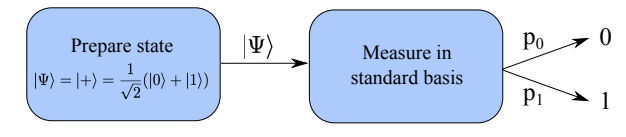
\includegraphics[width=1\linewidth]{Images/randomness.png}
    \caption{Genuine randomness from the preparation of a qubit in superposition}
    \label{fig:randomness}
\end{figure}
This simple example already tells us something about the power of quantum information: We could
build a machine that deterministically prepares the qubit $\ket{+}$, followed by a measurement in the
standard basis. Since $p_0=p_1=1/2$, this machine allows us to produce a perfect random number -
even though no randomness has been used inside our machine! In contrast, one can prove that no
classical deterministic machine can produce random numbers from scratch.

We saw how to measure a single qubit in the standard basis. The rule for computing probabilities
of measurement outcomes generalizes in a direct way to measuring n-qubit states. Indeed, consider
an n-qubit quantum state
\[
\ket{\Psi}=\sum_{x\in\{0,1\}^n} \alpha_x\ket{x}
\]
What happens when $\ket{\Psi}$ is measured in the standard basis $\ket{x}_x$? It turns out that the probability
of outcome x is given by $p_x = |\braket{x|\Psi}|^2=|\alpha_x|^2$, explaining again the need for normalization of
the vector $\ket{\Psi}$.

\subsubsection{Measuring a qubit in other bases}
Can we measure our qubit in any other basis? The answer to this is yes! Indeed this is another
feature that distinguishes quantum from classical, where the only basis around is the standard basis.
To find out how to analyze such a more general setting, let us first take a step back and consider
how we found the probabilities above. When measuring in the standard basis, the probabilities are given by the squared amplitudes when writing out the state in terms of the standard basis. When
measuring a qubit in a different orthonormal basis, given by vectors $\mathcal{G}=\{\ket{v},\ket{v^\perp}\}$, it is intuitive that we would have to express the qubit in the new basis. That is, we need to find amplitudes $\hat{\alpha}$ and $\hat{\beta}$ such that
\[
\ket{\psi}=\alpha\ket{0}+\beta\ket{1}=\hat{\alpha} \ket{v}+\hat{\beta}\ket{v^{\perp}}
\]
\begin{example}
    As an example, let consider again the qubit $\ket{+}=(1/\sqrt{2})(\ket{0}+\ket{1})$. Instead
of measuring it in the standard basis, let us now measure in the basis $H = \{\ket{+},\ket{-}\}$ given by
the two orthonormal vectors $\ket{+}$ and $\ket{-} = (1/\sqrt{2})(\ket{0}-\ket{1})$. Clearly, we can write the qubit as $1\ket{+}+0\ket{-}$. Thus the probability of obtaining measurement outcome “$\ket{+}$” is 1. We thus see
that the probabilities of measurement outcomes depends dramatically on the basis in which we
measure. 
\end{example}

\begin{example}
    Consider measuring an arbitrary qubit $\alpha\ket{0}+\beta\ket{1}$ in the basis $\{\ket{+},\ket{-}\}$. To
find out how to express the qubit in this other basis, it is convenient to determine how the basis
elements $\ket{0}$ and $\ket{1}$ look like in this basis. We find that
\[
\ket{0}=\frac{1}{2}[(\ket{0}+\ket{1})+(\ket{0}-\ket{1})]=\frac{1}{\sqrt{2}}(\ket{+}+\ket{-})
\]
\[
\ket{1}=\frac{1}{2}[(\ket{0}+\ket{1})-(\ket{0}-\ket{1})]=\frac{1}{\sqrt{2}}(\ket{+}-\ket{-})
\]
We thus have
\begin{align*}
\alpha\ket{0}+\beta\ket{1}&=\frac{1}{\sqrt{2}}[\alpha(\ket{+}+\ket{-})+\beta(\ket{+}-\ket{-})]\\
&=\frac{\alpha+\beta}{\sqrt{2}}\ket{+}+\frac{\alpha-\beta}{\sqrt{2}}\ket{-}
\end{align*}
This means that we obtain outcome "$\ket{+}$" with probability $|\alpha+\beta|^2/2$ and outcome "$\ket{-}$" with probability $|\alpha-\beta|^2/2$/
\end{example}

\begin{example}
    Consider the state $\ket{\Psi}=\ket{0}$. What are the probabilities  $p_0,p_1$ for measuring $\ket{\Psi}$ in the standard basis? What are the probability $p_{+},p_{-}$ for measuring $\ket{\Psi}$ in the Hadamard basis?
    For measuring in the standard basis the probabilities $p_0=1, p_1=0$. The probabilities in the Hadamard basis are $p_+=\frac{1}{2},p_-=\frac{1}{2}$.
\end{example}

Quite often we do not care about the entire probability distribution, but just the probability of one
specific outcome. Is there a more efficient way to find this probability than to rewrite the entire
state $\ket{\psi}$ in another basis? To investigate this, let us consider a single qubit
\[
\ket{\psi}=\alpha\ket{0}+\beta\ket{1}
\]
Remember that the elements of the standard basis are orthonormal. This means that
\[
(\ket{0})^{\dagger}\ket{0}=\begin{pmatrix} 1 & 0 \end{pmatrix}\begin{pmatrix} 1 \\ 0 \end{pmatrix} = 1,
\]
\[
(\ket{0})^{\dagger}\ket{1}=\begin{pmatrix} 1 & 0 \end{pmatrix}\begin{pmatrix} 0 \\ 1 \end{pmatrix} = 0
\]
Because the vectors are orthonormal, we could thus have found the desired probabilities by simply
computing the inner product between two vectors, as claimed above. Specifically, when given the qubit $\ket{\psi}=\alpha\ket{0}+\beta\ket{1}$ we obtain outcomes "$\ket{0}$" and "$\ket{1}$" with probabilities
\[
p_0=|\braket{0|\psi}|^2=\begin{vmatrix}\begin{pmatrix} 1 & 0 \end{pmatrix} \begin{pmatrix}\alpha \\ \beta \end{pmatrix}  \end{vmatrix}^2=|\alpha|^2
\]
\[
p_1=|\braket{1|\psi}|^2=\begin{vmatrix} \begin{pmatrix} 0 & 1 \end{pmatrix}\begin{pmatrix}\alpha \\ \beta \end{pmatrix}  \end{vmatrix}^2=|\beta|^2
\]

\begin{example}
    Suppose we measure $\ket{0}$ in the hadamard basis $\mathcal{H}$ (see above). The probabilities of observing outcomes "$\ket{+}$" and "$\ket{-}$" are given by
    \[
    p_+=|\braket{0|\psi}|^2=\begin{vmatrix}\begin{pmatrix} 1/\sqrt{2} & 1/\sqrt{2} \end{pmatrix} \begin{pmatrix}\alpha \\ \beta \end{pmatrix}  \end{vmatrix}^2=\frac{1}{2}
\]
\[
p_-=|\braket{1|\psi}|^2=\begin{vmatrix} \begin{pmatrix} 1/\sqrt{2} & 1/\sqrt{2} \end{pmatrix}\begin{pmatrix}\alpha \\ \beta \end{pmatrix}  \end{vmatrix}^2=\frac{1}{2}
\]
For multiple qubits, the rules for finding probabilities is analogous.
\end{example}

\begin{definition}
    Suppose that we measure a quantum state $\ket{\psi}$ in the orthonormal basis $\{\ket{b_j}\}_{j=1}^d$. The probability of observing outcome "$b_j$" can be found by computing
    \[
    p_j=|\braket{b_j|\psi}|^2
    \]
    The post-measurement state when obtaining outcome"$b_j$" is given by $\ket{b_j}$.
\end{definition}

Let us now consider some examples to gain intuition on measuring quantum systems in different
bases. First, let us have a look at a single qubit example.

\begin{example}
    Consider the qubit $\ket{\Psi}=\frac{1}{\sqrt{2}}(\ket{0}+\iota\ket{1})$, and measure the qubit in the $\{\ket{+},\ket{-}\}$ basis. the probabilities of obtaining "+" and "-" can be evaluated as follows:
    \begin{align*}
    p_+&=|\braket{\Psi|+}|^2=\begin{vmatrix} \dfrac{1}{2}(\bra{0}-\iota \bra{1})(\ket{0}+\ket{1})\end{vmatrix}^2\\
    &=\frac{1}{4}\begin{vmatrix} \braket{0|0}+\braket{0|1} - \iota\braket{1|0} - \iota \braket{1|1} \end{vmatrix}^2\\
    &=\frac{1}{4}|1-\iota|^2\\
    &=\frac{1}{4}(1-\iota)(1+\iota)=\frac{1}{2}
    \end{align*}
    \begin{align*}
    p_-&=|\braket{\Psi|-}|^2=\begin{vmatrix} \frac{1}{2}(\bra{0}-\iota \bra{1})(\ket{0}-\ket{1})\end{vmatrix}^2\\
    &=\frac{1}{4}\begin{vmatrix} \braket{0|0}+\braket{0|1} - \iota\braket{1|0} + \iota \braket{1|1} \end{vmatrix}^2\\
    &=\frac{1}{4}|1+\iota|^2\\
    &=\frac{1}{4}(1-\iota)(1+\iota)=\frac{1}{2}
    \end{align*}
\end{example}
This example shows that when the states involved have complex-valued amplitudes, one has to
take extra caution when evaluating the inner product: namely when taking the bra $\bra{\Psi}$, one should remember to alter the +/- sign whenever a complex number is involved (since the bra $\bra{\Psi}$ is the
conjugate transpose of the ket $\ket{\Psi}$). 

While we will generally talk about n-qubits, we can of course also consider a quantum system
comprised of three levels $\ket{0}$, $\ket{1}$, and $\ket{2}$, i.e. a qutrit. The rule for obtaining the probabilities of
measurement outcomes remains unchanged.

\begin{example}
    Consider a qutrit, which is a 3-dimensional quantum system represented by the vector
    \[
    \ket{v}=\frac{1}{\sqrt{2}}\begin{pmatrix} 1 \\ 0 \\ 0\end{pmatrix} + \frac{1}{\sqrt{2}}\begin{pmatrix} 0 \\ 1 \\ 0\end{pmatrix}\frac{1}{\sqrt{2}}\begin{pmatrix} 0 \\ 0 \\ 1\end{pmatrix}
    \]
    and measure in the basis $\mathcal{B}=\{\ket{b_1},\ket{b_2},\ket{b_3}\}$ where
    \[
    \ket{b_1}=\begin{pmatrix} 1 \\ 0 \\ 0 \end{pmatrix}, \quad \ket{b_2} = \frac{1}{\sqrt{2}}\begin{pmatrix} 0 \\ 1 \\ 1 \end{pmatrix}, \quad \frac{1}{\sqrt{2}}\begin{pmatrix} 0 \\ 1 \\ -1 \end{pmatrix} 
    \]
    The probabilities of obtaining each outcome can be calculated as follows:
    \[
    p_{b_1}=|\braket{b_1|v}|^2=\frac{1}{2}
    \]
    \[
    p_{b_2}=|\braket{b_2|v}|^2=\braket{b_2|v}\braket{v|b_2}=\frac{1}{2\sqrt{2}}(1+1)\frac{1}{2\sqrt{2}}(1+1)=\frac{1}{2}
    \]
    \[
    p_{b_3}=|\braket{b_3|v}|^2=\braket{b_3|v}\braket{v|b_3}|=\frac{1}{2\sqrt{2}}(1-1)\frac{1}{2\sqrt{2}}(1-1)=0
    \]
\end{example}

\subsubsection{Measurement Example I: Phase Estimation}
Now that we have discussed qubits in some detail, we can are prepared to
look more closesly at the measurement principle. Consider the quantum
state,
|\[
\ket{\psi}=\frac{1}{\sqrt{2}}\ket{0}+\frac{e^{\iota\theta}}{\sqrt{2}}\ket{1}
\]
If we were to measure this qubit in the standard basis, the outcome would
be $0$ with probability $1/2$ and $1$ with probability$ 1/2$. This measurement
tells us only about the norms of the state amplitudes. Is there any measurement that yields information about the phase, $\theta$?
To see if we can gather any phase information, let us consider a measurement in a basis other than the standard basis, namely
\[
\ket{+}=\frac{1}{\sqrt{2}}(\ket{0}+\ket{1}) \quad \text{and}\quad \ket{-}=\frac{1}{\sqrt{2}}(\ket{0}-\ket{1})
\]
What does $\ket{\phi}$ look like in this new basis? This can be expressed by first
writing,
\[
\ket{0}=\frac{1}{\sqrt{2}}(\ket{+}+\ket{-}) \quad \text{and} \quad \ket{-}=\frac{1}{\sqrt{2}}(\ket{0}-\ket{1})
\]
Now we are equipped to rewrite $\ket{\psi}$ in the $\{\ket{+}$, $\ket{-}\}$-basis,
\begin{align*}
\ket{\psi}&=\frac{1}{\sqrt{2}}\ket{0}+\frac{e^{\iota\theta}}{\sqrt{2}}\ket{1}\\
&=\frac{1}{2}(\ket{+}+\ket{-})+\frac{e^{\iota\theta}}{\sqrt{2}}(\ket{+}-\ket{-})\\
&=\frac{1+e^{\iota\theta}}{2}\ket{+}+\frac{1-e^{\iota\theta}}{2}\ket{-}
\end{align*}
Recalling the Euler relation, $e^{\iota theta}=\cos \theta+\iota\sin \theta$, we see that the probability
of measuring $\ket{+}$ is $\frac{1}{4}((1+\cos \theta)^2+\sin^2 \theta)=\cos^2 (\theta/2)$. A similar calculation reveals that the probability of measuring $\ket{-}$ is $\sin^2 (\theta/2)$ Measuring
in the ($ket{+},\ket{-}$)-basis therefore reveals some information about the phase $\theta$.
Later we shall show how to analyze the measurement of a qubit in a
general basis.

\subsubsection{Measurement example II: general Qubit Bases}
What is the result of measuring a general qubit state $\ket{\psi}=\alpha\ket{0}+\beta\ket{1}$, in
a general orthonormal basis $\ket{v}$, $\ket{v^{\perp}}$, where $\ket{v}=a\ket{0}+b\ket{1}$ and $\ket{v^{\perp}}=b^*\ket{0}-a^*\ket{1}$? You should also check that $\ket{v}$ and $\ket{v^{\perp}}$ are orthogonal by
showing that $\braket{v|v^{\perp}}=0$.

To answer this question, let us make use of our recently acquired braket notation. We first show that the states $\ket{v}$ and $\ket{v^{\perp}}$ are orthogonal, that is, that their inner product is zero:
\begin{align*}
\braket{v|v^{\perp}}&=(b^*\ket{0}-a^*\ket{1})^{\dagger}(a\ket{0}+b\ket{1})\\
&=(b\bra{0}-a\bra{1})^{\dagger}(a\ket{0}+b\ket{1})\\
&=ba\braket{0|0}-a^2\braket{1|0}+b^2\braket{0|1}-ab\braket{1|1}\\
&=ba-0+0-ab\\
&=0
\end{align*}

Here we have used the fact that $\braket{i|j}=\delta_{ij}$ .

Now, the probability of measuring the state $\ket{\psi}$ and getting $\ket{v}$ as a
result is,
\begin{align*}
p_{\psi}(v)&=|\braket{v|\psi}|^2\\
&=|(a^*\bra{0}+b^*\bra{1})(\alpha\ket{0}+\beta\ket{1})|^2\\
&=|a^*\alpha+b^*\beta|^2
\end{align*}
Similarly,
\begin{align*}
P_{\psi}(v^{\perp})&=|\braket{v^{\perp}|\psi}|^2\\
&=|(b\bra{0}-a\bra{1})(\alpha\ket{0}+\beta\ket{1})|^2\\
&=|b\alpha-\alpha\beta|^2
\end{align*}

\subsubsection{Expectation Values}
Physicists (but also computer scientists!) like to compute expectation values of measurement outcomes, as they provide an indication of the average behavior, if one was to perform a measurement many times (however we shall see later, that the measurement will perturb the state!). let us suppose that we measure a qubit $\ket{\Psi}$ in the standard basis $\{\ket{0},\ket{1}\}$. We will adopt the physics convention of labelling outcomes $\pm1$. This means that we associate the outcome "$\ket{0}$" with outcome $+1$, and outcome "$\ket{1}$" with outcome $-1$. The expectation value the outcome obtained when measuring $\ket{\psi}$ is then
\[
E=1|\braket{0|\psi}|^2-1\braket{1|\psi}|^2
\]
Note that since $|\braket{0|\psi}|^2=\braket{\psi|0}\braket{0|\psi}$, we have
\[
E=\bra{\psi}(\ket{0}\bra{0}-\ket{1}\bra{1})\ket{\psi}=\braket{\psi|Z|\psi}
\]
where $Z=\ket{0}\bra{0}-\ket{1}\bra{1}$.  As we shall see later, $Z$ is called the Pauli-Z matrix.

\subsection{Measuring Multiple Systems}
We saw how to measure some quantum state $\ket{\psi}$. let us now consider what happens if we measure the state of multiple qubits, where we think of measuring each qubit in a separate basis. To understand this, it is useful to realize that a basis for the join state space $\mathbb{C}_A^{d_A} \otimes \mathbb{C}_B^{d_B}$ can be obtained from bases for the individual state spaces $\mathbb{C}_A^{d_A}$ and $\mathbb{C}_B^{d_B}$. Specifically, if $\{\ket{b_j^A}\}_j$ is basis for $\mathbb{C}_A^{d_A}$ and $\{\ket{b_j^B}\}_j$ is a basis for the state space $\mathbb{C}_B^{d_B}$, then the set of vectors $\{\{\ket{b_j^A}\otimes \ket{b_k^B}\}_{j=1}^{d_A}\}_{k=1}^{d_B}$ gives a basis for $\mathbb{C}_A^{d_A}\otimes \mathbb{C}_B^{d_B}$.

\begin{example}
    Consider the basis $\{\ket{0}_A,\ket{1}_A\}$ for qubit A, and the basis \\$\{\ket{+}_B,\ket{-}_B\}$ for qubit B. A basis for the joint state AB is then given by \\
    $\{\ket{0}_A\ket{+}_B,\ket{0}_A\ket{-}_B,\ket{1}_A\ket{+}_B,\ket{1}_A\ket{-}_B\}$.
\end{example}

Let us not think how we might construct how we might construct some measurement for two quantum states from measurements of the individual ones. Suppose we measure particle A in the basis $\{\ket{b_j^A}\}_j$ and particle B in the basis $\{b_k^B\}_k$ when the joint state of both particles is given by $\ket{\psi}_{AB}$. What is the probability that we obtain outcome "$\ket{b_j^A}$" on A, and outcome "$\ket{b_k^B}$" on B? To find such joint probabilities, we first write down the joint basis fo quantum states A and B as above: $\{\{\ket{b_j^A}\ket{b_k^B}\}_j\}_k$. We can apply the usual rule to compute the probability as 
\[
p_{jk}=|\braket{b_j^A|\braket{b_k^B|\ket{\psi}_{AB}}}|^2
\]
\begin{example}
    Consider the two qubits in an EPR pair
    \[
    \ket{EPR}=\frac{1}{\sqrt{2}}(\ket{00}+\ket{11}
    \]
    and measure them both in the standard basis. The probabilities of obtaining outcomes 00, 01 ,10 and 11 are given by
    \[
    p_{00}=p_{11}=\frac{1}{2}
    \]
    \[
    p_{01}=p_{10}=0
    \]
\end{example}

\subsubsection{Partial Measurements}
Suppose we have a system consisting of two or more qubits and we only measure one of them. For
example, suppose the qubits are X and Y, and these qubits are in the state
\[
\ket{\psi}=\frac{1}{2}\ket{00}-\frac{\iota}{2}\ket{10}+\frac{1}{\sqrt{2}}\ket{11}
\]
We know what the distribution of measurement outcomes would be if we measured both qubits:
\[
Pr\text{[outcome is 00]} = \frac{1}{4} \quad Pr\text{[outcome is 01]}=0
\]
\[
Pr\text{[outcome is 10]}=\frac{1}{4} \quad pr\text{[outcome is 11]}=\frac{1}{2}
\]
The probability that a measurement of the first qubit, for instance, results in outcome $0$ should
therefore be $1/4+0 = 1/4$ and the probability of outcome $1$ should be $1/4+1/2 = 3/4$. Intuitively,
this should be the case regardless of whether or not the second qubit was actually measured. Indeed
this is the case.

However, what is different between the case where the second qubit is measured and the case
where it is not is the superposition of the system after the measurement (or measurements). If both
qubits are measured, the superposition will be one of $\ket{00},\ket{01},\ket{10}$, or $\ket{11}$, depending on the
measurement outcome. If only the first qubit is measured, however, this may not be the case.
I’ll explain how you determine the state of the system after the measurement of the first qubit
for the example above, and the method for a general case should be clear. We begin by considering
the possible outcome 0 for the measurement. We consider the state
\[
\ket{\psi}=\frac{1}{2}\ket{00}-\frac{\iota}{2}\ket{10}+\frac{1}{\sqrt{2}}\ket{11}
\]
and cross off all of the terms in the sum that are inconsistent with measuring a $0$ for the first qubit:
\[
\ket{\psi}=\frac{1}{2}\ket{00}
\]
which leaves
\[
\frac{1}{\ket{00}}
\]
The probability of measuring 0 is the norm-squared of this vector.
\[
Pr\text{[measurement outcomes is 0]}=|\\frac{1}{2}\ket{00}\|=\frac{1}{4}
\]
and the state of the two qubits after the measurement conditioned on the measurement outcome being 0 is the vector itself renormalized:
\[
\frac{\frac{1}{2}\ket{00}}{\|\frac{1}{2}\ket{00}\|}=\ket{00}
\]
The possible measurement outcome 1 is handled similarly. we cross off the terms is inconsistent with measuring a 1 which leaves
\[
-\frac{\iota}{2}\ket{10}+\frac{1}{\sqrt{2}}\ket{11}
\]
The probability of measuring a 1 is then the norm-squared of this vector,
\[
Pr\text{measurement outcome is 1]}=\|-\frac{\iota}{2}\ket{10}+\frac{1}{\sqrt{2}}\ket{11}\|^2=|-\frac{\iota}{2}|^2+|\frac{1}{\sqrt{2}}|^2=\frac{3}{4}
\]
and conditioned on measuring a 1 is then the norm-squared of this vector
\[
\frac{-\frac{\iota}{2}\ket{10}+\frac{1}{\sqrt{2}}\ket{11}}{\|-\frac{\iota}{2}\ket{10}+\frac{1}{\sqrt{2}}\ket{11}\|}=-\frac{\iota}{\sqrt{3}}\ket{10}+\sqrt{\frac{2}{3}}\ket{11}
\]
A completely equivalent way of performing this calculation is to begin by writing
\[
\ket{\psi}=\ket{0}\ket{\phi_0}+\ket{1}\ket{\phi_1}
\]
for some choice of $\ket{\phi_0}$ and $\ket{\phi_1}$. (There will always be a unique choice for each that works.) in this case we have
\[
\ket{\psi}=\ket{0}\left(\frac{1}{2}\ket{0}\right)+\ket{1}\left(-\frac{\iota}{2}\ket{0}+\frac{1}{\sqrt{2}}\ket{1}\right)
\]
so $\ket{\phi_0}=\frac{1}{2}\ket{0}$ and $\ket{\phi_1}=-\frac{\iota}{2}\ket{0}+\frac{1}{\sqrt{2}}\ket{1}$. The probabilities for the two measurement outcomes are as follows:
\[
Pr\text{[outcome is 0]}=\|\ket{\phi_0}\|^2=|\frac{1}{2}|^2=\frac{1}{4}
\]
\[
Pr\text{[outcome is 1]}=\|\ket{\phi_1}\|^2=|-\frac{\iota}{2}|^2+|\frac{1}{\sqrt{2}}|^2=\frac{3}{4}
\]
Conditioned on the measurement outcome, the state of the two qubits is as follows:
\[
\text{measurement outcome is 0}\implies \text{state becomes} \frac{1}{\|\ket{\phi_0}\|}\ket{0}\ket{\phi_0}=\ket{00}
\]
\[
\text{measurement outcome is 1} \implies \text{state becomes}\frac{1}{\|\ket{\phi_1}}\ket{1}\ket{\phi_1}=\frac{-\iota}{\sqrt{3}}\ket{10}+\sqrt{\frac{2}{3}}\ket{11}
\]
The same method works for more than 2 qubits as well.

\begin{example}
    Suppose 3 qubits are in the superposition
    \[\ket{\psi}=\frac{1}{2}\ket{000}+\frac{1}{2}\ket{100}+\frac{1}{2}\ket{101}-\frac{1}{2}\ket{111}\]
    and the third qubit is measured. What are the probabilities of the two possible measurement outcomes and what are the resulting superpositions of the three qubits for each case?
    To determine the answer we ewrite,
    \[
    \ket{\psi}=\left(\frac{1}{2}\ket{00}+\frac{1}{2}\ket{10}\right)\ket{0}+\left(\frac{1}{2}\ket{10}-\frac{1}{2}\ket{11}\right)\ket{1}
    \]
    The probability that the measurement outcome is 0 is
    \[
    \|\frac{1}{2}\ket{00}+\frac{1}{2}\ket{10}\|^2=\frac{1}{2}
    \]
    and in this case the resulting superposition is 
    \[
    \sqrt{2}\left(\frac{1}{2}\ket{00}+\frac{1}{2}\ket{10}\right)\ket{0}=\frac{1}{\sqrt{2}}\ket{000}+\frac{1}{\sqrt{2}}\ket{100}
    \]
    The probability that the measurement outcome is 1 is
    \[
    \|\frac{1}{2}\ket{10}-\frac{1}{2}\ket{11}\|^2=\frac{1}{2}
    \]
    and in this case the resulting superposition is
    \[
    \sqrt{2}\left(\frac{1}{2}\ket{10}-\frac{1}{2}\ket{11}\right)\ket{1}=\frac{1}{\sqrt{2}}\ket{101}-\frac{1}{\sqrt{2}}\ket{111}
    \]
\end{example}
\section{The Stern-Gerlach Experiment}
The concepts of superposition and entanglement are counter-intuitive to our daily experiences. The following experiment proves that the nature truly operates in this peculiar manner. It provides the proof for existence of qubits in Nature. thus, showing that the relalization of large-scale quantum computers will be experimentally feasible.

The qubit is a fundamental element for quantum computation and quantum information. An early experiment indicating the qubit structured was performed by Stern in 1921 and Gerlach in 1922 in frankfurt. In the original Stern-Gerlach Experiment, hot atoms were 'beamed' from an oven through a magnetic filed which caused the atoms to be deflected, and then the position of each atom was recorded. The original experiment was done with silver atoms, which have a complicated structure that obscures the effects we are discussing. What we describe below actually follows a 1927 experiment done using hydrogen atoms. The same basic effect is observed, but with hydrogen atoms the discussion is easier to follow. Keep in mind, though, that this privilege wasn't available to people in the early 1920s, and they have to be very ingenious to think up explanations for the more complicated effects they observed.

Hydrogen atoms contain a proton and an orbiting electron. you can think of this electron as a little 'electric current' around the proton. This electric current causes the atom to have a magnetic filed; each atom has what physicists call a `magnetic dipole moment'. As a result each atom behaves like a little bar magnet with an axis corresponding to the axis the electron is spinning around. throwing little bar magnet is through a magnetic filed causes the magnets to be deflected by the field, and we expect to see a similar deflection of atoms in the Stern-Gerlach experiment.

How the atom is deflected depends upon both the atom's magnetic dipole moment - the axis the electron is spinning around and the magnetic filed generated by the Stern-Gerlach device. We won't go through the details, but suffice to say that by constructing the Stern-Gerlach device appropriately, we can cause the atom to be deflected by an amount that depends upon the $\hat{z}$ component of the atom's magnetic dipole moment, where $\hat{z}$ is some fixed external axis.

Two major surprises emerge when this experiment is performed. First, since the hot atoms exiting the oven would naturally be expected to have their dipoles oriented randomly in every direction, it would follow that there would be a continuous distribution of atoms seen at all angles exiting from the Stern-gerlach device. Instead, what is seen is atoms emerging from a discrete set of angles. Physicists were able to explain this by assuming that the magnetic dipole moment of atoms is quantized, that is, comes in discrete multiples of some fundamental amount.

This observation of quantization in the Stern-Gerlach experiment was surprising to physicists of the 1920s, but not completely astonishing because evidence of quantization effects in other systems was becoming widespread at that time. What was truly surprising was the number of peaks seen in the experiment. The hydrogen atoms being used were such that they should have zero magnetic dipole moment. Classically, this is surprising in itself, since it corresponds to no orbital motion of the electron, but based on what was known of quantum mechanics at that time was an acceptable notion. Since the hydrogen atoms would therefore have zero magnetic moment, it was expected that only one beam of atoms would be seen, and this beam would not be deflected by the magnetic field. instead, two beams were seen, one deflected up by the magnetic field and the other deflected down.

This puzzling doubling was explained after considerable effort by positioning that the electron in the hydrogen atoms has associated with it a quantity called spin. This spin is not in any way associated to the usual rotational motion of the electron around the proton; it is an entirely new quantity associated with with an electron. The great physicist Heisenberg labeled the idea `brave' at the time it was suggested, and it is a brave idea, since it introduces an essentially new physical quantity into Nature. The spin of the electron is posited to make an extra contribution to the magnetic dipole moment of a hydrogen atom, in addition to the contribution due to the rotational motion of the electron.
\begin{figure}
    \centering
    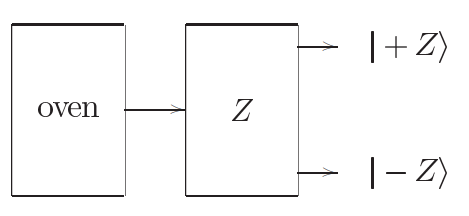
\includegraphics[width=0.5\linewidth]{Images/stern-gerlach.png}
    \caption{Abstract schematic of Stern-Gerlach experiment. Hot hydrogen atoms are beamed from an oven through a magnetic field, causing a deflection either up $(\ket{+Z})$ or down $(\ket{-Z})$}
    \label{fig:abs-sgexp}
\end{figure}
What is the proper description of the spin of the electron? As a first guess, we might hypothesize that the spin is specified by a single bit, telling the hydrogen atom to go up or down. Additional experimental results provide further useful information to determine if this guess needs refinement or replacement. Let's represent the original Stern-Gerlach apparatus as shown in the figure \ref{fig:3stage-sgexp}. Its outputs are two beams of atoms, which we shall called $\ket{+Z}$ and $\ket{-Z}$. (We're using suggestive notation which looks quantum mechanics, but of course you're free to use whatever notation you prefer). Now suppose we cascade two Stern-Gerlach apparatus together, as shown in the figure \ref{fig:casc-sgexp}. We arrange it so that the second apparatus is tipped sideways, so the magnetic field deflects the atoms along the $\hat{x}$ axis. In our thought-experiment we'll block off the $\ket{-Z}$ output from the first Stern-Gerlach apparatus, while the $\ket{+Z}$ output is sent through a second apparatus oriented along the $\hat{x}$ axis. A detector is placed at the final output to measure the distribution of atoms along the $\hat{x}$ axis.

A classical magnetic dipole pointed in the $+\hat{z}$ direction has no net magnetic moment in the $\hat{x}$ direction, so we might expect that the final output would have one central peak. However, experimentally it is observed that there are two peaks of equal intensity! So perhaps these atoms are peculiar, and have definite magnetic moments along each axis, independently. That is, maybe each atom passing through the second apparatus can be described as being in a state we might write as $\ket{+Z}\ket{+X}$ or $\ket{+Z}\ket{-X}$, to indicate the two values for spin that might be observed. 
\begin{figure}
    \centering
    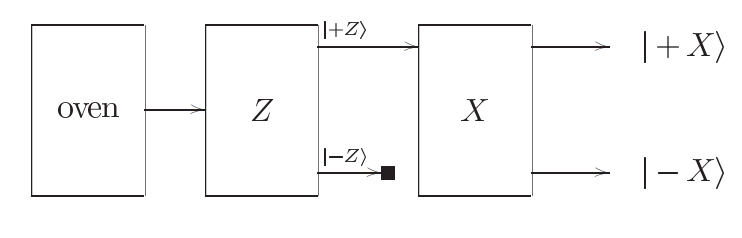
\includegraphics[width=0.65\linewidth]{Images/casca_sgexp.png}
    \caption{Cascaded Stern-gerlach Experiment}
    \label{fig:casc-sgexp}
\end{figure}
\begin{figure}
    \centering
    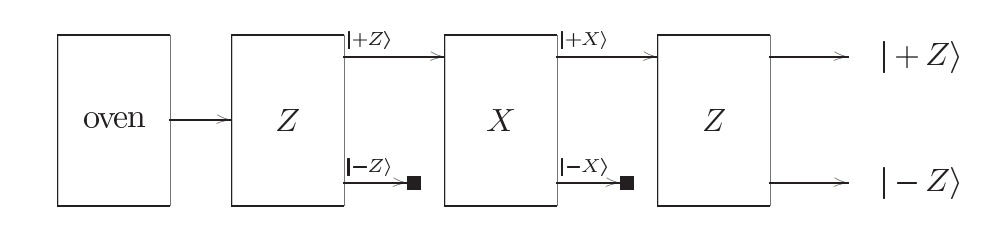
\includegraphics[width=0.75\linewidth]{Images/3stage-sgexp.png}
    \caption{Three stage cascaded Stern-Gerlach measurements}
    \label{fig:3stage-sgexp}
\end{figure}
Another experiment, shown in figure \ref{fig:casc-sgexp}, can test this hypothesis by sending one beam of the previous output through a second $\hat{z}$ oriented Stern-Gerlach apparatus. If the atoms had retained their $\ket{+Z}$ orientation, then the output would be expected to have only one peak at the $\ket{+Z}$ output. However, again tow beams are observed at the final output, of equal intensity. Thus, the conclusion would seem to be that contrary to classical expectations, a $\ket{+Z}$ state consists of equal portions of $\ket{+Z}$ and $\ket{-X}$ states, and a $\ket{+X}$ state consists of equal portions of $\ket{+Z}$ and $\ket{-Z}$ states. Similar conclusions can be reached if the Stern-Gerlach apparatus is aligned along some other axis like the $\hat{y}$ axis.

The qubit model provides a simple explanation of this experimentally observed behavior. Let $\ket{0}$ and $\ket{1}$ be the states of a qubit, and make the assignments.
\begin{align*}
    \ket{+Z} &\leftarrow \ket{0}\\
    \ket{-Z} &\leftarrow \ket{1}\\
    \ket{+X} &\leftarrow (\ket{0}+\ket{1})/\sqrt{2}\\
    \ket{-X} &\leftarrow (\ket{0}- \ket{1})/\sqrt{2}
\end{align*}
then the results of the cascaded Stern-Gerlach experiment can be explained by assuming that the $\hat{z}$ Stern-Gerlach apparatus measures the spin (that is, the qubit) in the computational $\ket{0},\ket{1}$, and the $\hat{x}$ Stern-Gerlach apparatus measures the spin with respect to the basis $(\ket{0}+\ket{1})/\sqrt{2}, (\ket{0}-\ket{1})/\sqrt{2}$. For example, in the cascaded $\hat{z}-\hat{x}-\hat{z}$ experiment, if we assume that the spin are in the state $\ket{+Z}=\ket{0}=(\ket{+X}+\ket{-X})/\sqrt{2}$ after exiting the first Stern-gerlach experiment, then the probability for obtaining $\ket{+X}$ out of the second apparatus is $1/2$, and the probability for $\ket{-X}$ is 1/2. Similarly, the probability for obtaining $\ket{+Z}$ out of the third apparatus is $1/2$. A qubit model thus properly predicts results from this type of cascaded Stern-Gerlach experiment.

This example demonstrates how qubits could be a believable way of modelling systems in Nature. Of course it doesn't establish beyond all doubt that the qubit model is the correct way of understanding electron spin - far more experimental corroboration is required. nevertheless, because of many experiments like these, we now believe that the qubit model (and generalizations of it to higher dimensions; quantum mechanics in other words) is capable of describing every physical system.

\section{Qiskit Examples}
In this section we present some examples of Qiskit implementations of the concepts introduced in this lesson.

\subsection{Vector and Matrices in Python}
Qiskit uses the Python programming language, so before discussing Qiskit specifically it may be helpful to very briefly discuss matrix and vector computations in Python. In Python, matrix and vector computations can be performed using the  array  class from the  NumPy  library (which includes many additional components for numerical computation).

Here is an example of a code cell that defines two vectors,  ket0  and  ket1, corresponding to the qubit state vectors $\ket{0}$ and $\ket{1}$ and displays their average.
\begin{lstlisting}[language=Python]
from numpy import array

ket0 = array([1, 0])
ket1 = array([0, 1])

display(ket0 / 2 + ket1 / 2)
\end{lstlisting}
Output:
\begin{lstlisting}
array([0.5, 0.5])
\end{lstlisting}
It is not actually necessary to explicitly use the  display  command to see the result of this computation. We may instead simply write the expression of interest as the last line of the code cell, and it will be returned as its output:
\begin{lstlisting}[language=Python]
ket0 / 2 + ket1 / 2
\end{lstlisting}
Output:
\begin{lstlisting}
array([0.5, 0.5])
\end{lstlisting}

This code cell also illustrates that running code cells sequentially on a given page of this textbook has a cumulative effect, so it is not necessary to reload the  array  class or define ket0  and  ket1  again. Reloading the page or switching to another page will, however, reset everything to its initial state.

As a general guideline, code cells within each subsection of this course are intended to be run sequentially. So, if running a code cell generates an error, be sure to first run all previous code cells within the subsection in which that code cell appears.

We can also use  array  to create matrices that represent operations.
\begin{lstlisting}[language=Python]
M1 = array([[1, 1], [0, 0]])
M2 = array([[1, 1], [1, 0]])

M1 / 2 + M2 / 2
\end{lstlisting}
Output:
\begin{lstlisting}
array([[1. , 1. ],
       [0.5, 0. ]])
\end{lstlisting}
Matrix multiplication (including matrix-vector multiplication as a special case) can be performed using the  matmul  function from  NumPy  :
\begin{lstlisting}[language=Python]
from numpy import matmul

display(matmul(M1, ket1))
display(matmul(M1, M2))
display(matmul(M2, M1))
\end{lstlisting}
Output:
\begin{lstlisting}
array([1, 0])
array([[2, 1],
       [0, 0]])
array([[1, 1],
       [1, 1]])
\end{lstlisting}

\subsection{States, measurements and operations}
Qiskit includes several classes that allow for states, measurements, and operations to be easily created and manipulated — so starting from scratch and programming everything that is needed to simulate quantum states, measurements, and operations in Python is not required. Some examples to get started are included below.

\subsubsection{Defining and displaying state vectors}

Qiskit's  Statevector  class provides functionality for defining and manipulating quantum state vectors. The following code cell imports the  Statevector  class and defines a few vectors using it. (Note that we need the  sqrt  function from the  NumPy  library to compute the square roots for the vector  u .)
\begin{lstlisting}[language=Python]
from qiskit.quantum_info import Statevector
from numpy import sqrt

u = Statevector([1 / sqrt(2), 1 / sqrt(2)])
v = Statevector([(1 + 2.0j) / 3, -2 / 3])
w = Statevector([1 / 3, 2 / 3])

print("State vectors u, v, and w have been defined.")
\end{lstlisting}
Output:
\begin{lstlisting}
State vectors u, v, and w have been defined.
\end{lstlisting}

The  Statevector  class provides a  draw  method for displaying state vectors, including latex  and  text  options for different visualizations, as this code cell demonstrates:

\begin{lstlisting}[language=Python]
display(u.draw("latex"))
display(v.draw("text"))
\end{lstlisting}
Output:
\[
\frac{\sqrt{2}}{2}\ket{0}+\frac{\sqrt{2}}{2}\ket{1}
\]
\[
[ 0.33333333+0.66666667j,-0.66666667+0.j ]
\]
The  Statevector  class also includes the  is\_valid  method, which checks to see if a given vector is a valid quantum state vector (i.e., that it has Euclidean norm equal to 1):
\begin{lstlisting}[language=Python]
display(u.is_valid())
display(w.is_valid())
\end{lstlisting}
Output:
\begin{lstlisting}
True

False
\end{lstlisting}
\subsubsection{Simulating Measurements using Statevector}
Next we will see one way that measurements of quantum states can be simulated in Qiskit, using the  measure  method from the  Statevector  class.

First, we create a qubit state vector  v  and then display it.
\begin{lstlisting}[language=Python]
v = Statevector([(1 + 2.0j) / 3, -2 / 3])
v.draw("latex")
\end{lstlisting}
Output:
\[
\left(\frac{1}{3}+\frac{2\iota}{3}\right)\ket{0}-\frac{2}{3}\ket{1}
\]
Next, running the  measure  method simulates a standard basis measurement. It returns the result of that measurement, plus the new quantum state of our system after that measurement
\begin{lstlisting}[language=Python]
v.measure()
\end{lstlisting}
Output:
\begin{lstlisting}
('1',
 Statevector([ 0.+0.j, -1.+0.j],
             dims=(2,)))
\end{lstlisting}
Measurement outcomes are probabilistic, so the same method can return different results. Try running the cell a few times to see this. 

For the particular example of the vector v, defined above, the measure method defines the quantum state vector after the measurement takes place to be
\[
\frac{1+2\iota}{\sqrt{5}}\ket{0}
\]
(rather than $\ket{0}$) or
\[
-\ket{1}
\]
(rather than $\ket{1}$), depending on the measurement outcome. In bot cases, the alternatives are, in fact, equivalent - they are said to differ by a global phase because one is equal to the other multiplied by a complex number on the unit circle. This issue is discussed in greater detail in the next chapter.

As an aside, Statevector will throw an error if the measure method is applied to an invalid quantum state vector. Feel free to give it a try if you are interested in seeing what an error looks like.

State vector also comes with a sample\_counts method that allows for the simulation of any number of measurements on the system. For example, the following cell shows the outcome of measuring the vector v 1000 times, which (with high probability) results in the outcome 0 approximately 5 out of every 9 times (or about 556 of the 1000 trials) and the outcome 1 approximately 4 out of every 9 times (or about 444 out of the 100 trials). The cell also demonstrates the plot\_histogram function for visualizing the results.

\begin{lstlisting}[language=Python]
from qiskit.visualization import plot_histogram

statistics = v.sample_counts(1000)
display(statistics)
plot_histogram(statistics)
\end{lstlisting}
Output:
\begin{lstlisting}
{np.str_('0'): np.int64(568), np.str_('1'): np.int64(432)}
\end{lstlisting}

\begin{figure}[ht]
    \centering
    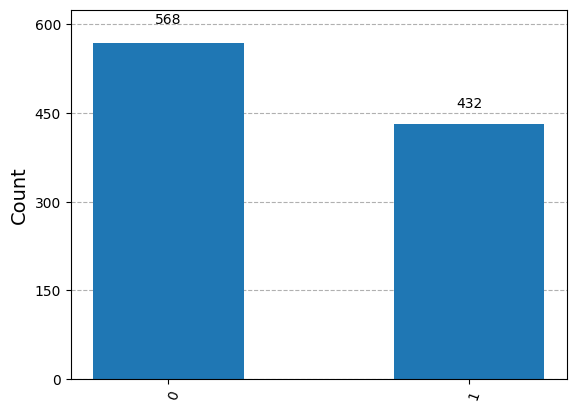
\includegraphics[width=0.75\textwidth]{Images/histogram_exp.png}
    \caption{Histogram of measurement outcomes}
\end{figure}

Running the cell multiple times and trying different numbers of samples in place of 1000 may be helpful for developing some intuition for how the number of trials influences the estimated probabilities.

\subsubsection{Performing operations with Operator and Statevector}
Unitary operations can be defined and performed on state vectors in Qiskit using the operator class, as in the example that follows:

\begin{lstlisting}[language=Python]
from qiskit.quantum_info import Operator

X = Operator([[0, 1], [1, 0]])
Y = Operator([[0, -1.0j], [1.0j, 0]])
Z = Operator([[1, 0], [0, -1]])
H = Operator([[1 / sqrt(2), 1 / sqrt(2)], [1 / sqrt(2), -1 / sqrt(2)]])
S = Operator([[1, 0], [0, 1.0j]])
T = Operator([[1, 0], [0, (1 + 1.0j) / sqrt(2)]])

v = Statevector([1, 0])

v = v.evolve(H)
v = v.evolve(T)
v = v.evolve(H)
v = v.evolve(T)
v = v.evolve(Z)

v.draw("text")
\end{lstlisting}
Output:
\begin{lstlisting}
[ 0.85355339+0.35355339j,-0.35355339+0.14644661j]
\end{lstlisting}

\subsubsection{Looking ahead toward Quantum Circuits}
Quantum circuits won't be formally introduced until the next few chapters, but we can nevertheless experiment with composing qubit unitary operations using Qiskit's QuantumCircuit class. In particular, we may define a quantum circuit (which in this case will simply be a sequence of unitary operations performed on a single qubit)

\begin{lstlisting}[language=Python]
from qiskit import QuantumCircuit

circuit = QuantumCircuit(1)

circuit.h(0)
circuit.t(0)
circuit.h(0)
circuit.t(0)
circuit.z(0)

circuit.draw()
\end{lstlisting}
Output:
\begin{figure}[ht]
    \centering
    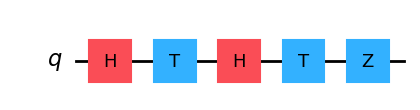
\includegraphics[width=0.75\textwidth]{Images/circuit_exp.png}
    \caption{Quantum Circuit}
\end{figure}
The operations are applied sequentially, starting on the left and ending on the right in the figure. Let us first initialize a starting quantum state vector and then evolve that state according to the sequence of operations.

\begin{lstlisting}[language=Python]
ket0 = Statevector([1, 0])
v = ket0.evolve(circuit)
v.draw("text")
\end{lstlisting}
Output:
\begin{lstlisting}
[ 0.85355339+0.35355339j,-0.35355339+0.14644661j]
\end{lstlisting}

Finally, let's simulate the result of running this experiment (i.e., preparing the state $\ket{0}$, applying the sequence of operations represented by the circuit, and measuring 4000 times.

\begin{lstlisting}[language=Python]
statistics = v.sample_counts(4000)
plot_histogram(statistics)
\end{lstlisting}
Output:
\begin{figure}[ht]
    \centering
    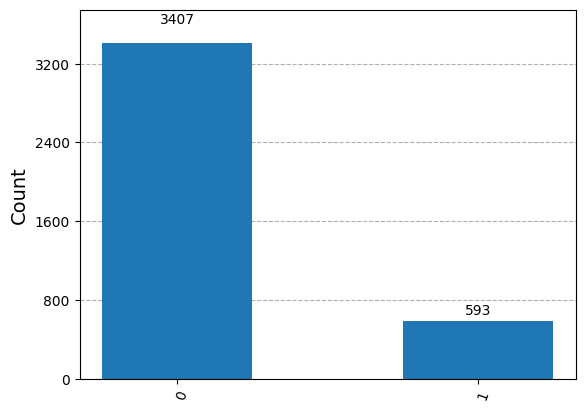
\includegraphics[width=0.75\textwidth]{Images/histogram_exp2.png}
    \caption{Histogram of measurement outcomes}
\end{figure}
In the previous lesson, we learned about Qiskit's Statevector and Operator classes, and used them to simulate quantum systems. In this section, we'll use them to explore the behavior of multiple systems. We'll start by importing these classes, as well as the square root function from NumPy .

\begin{lstlisting}[language=Python]
from qiskit.quantum_info import Statevector, Operator
from numpy import sqrt
\end{lstlisting}

\subsubsection{Tensor products}
The Statevector class has a tensor method which returns the tensor product of itself and another Statevector .

For example, below we create two state vectors representing $\ket{0}$ and $\ket{1}$, and use the tensor method to create a new vector, $\ket{0}\otimes \ket{1}$.
\begin{lstlisting}[language=Python]
zero, one = Statevector.from_label("0"), Statevector.from_label("1")
zero.tensor(one).draw("latex")
\end{lstlisting}
Output:
\[
\ket{01}
\]
In another example below, we create state vectors representing the 
$\ket{+}$ and $\frac{1}{\sqrt{2}}(\ket{0}+\iota\ket{1})$ states, and combine them to create a new state vector. We'll assign this new vector to the variable psi.
\begin{lstlisting}[language=Python]
plus = Statevector.from_label("+")
i_state = Statevector([1 / sqrt(2), 1j / sqrt(2)])
psi = plus.tensor(i_state)

psi.draw("latex")
\end{lstlisting}
Output:
\[
\frac{1}{2}\ket{00}+\frac{\iota}{2}\ket{01}+\frac{1}{2}\ket{10}+\frac{\iota}{2}\ket{11}
\]
The Operator class also has a tensor method. In the example below, we create the X and I gates and display their tensor product.
\begin{lstlisting}[language=Python]
X = Operator([[0, 1], [1, 0]])
I = Operator([[1, 0], [0, 1]])

X.tensor(I)
\end{lstlisting}
Output:
\begin{lstlisting}
Operator([[0.+0.j, 0.+0.j, 1.+0.j, 0.+0.j],
          [0.+0.j, 0.+0.j, 0.+0.j, 1.+0.j],
          [1.+0.j, 0.+0.j, 0.+0.j, 0.+0.j],
          [0.+0.j, 1.+0.j, 0.+0.j, 0.+0.j]],
         input_dims=(2, 2), output_dims=(2, 2))
\end{lstlisting}
We can then treat these compound states and operations as we did single systems in the previous lesson. For example, in the cell below we calculate $(I\otimes X)\ket{\psi}$ for the state psi we defined above. (The operator shown tensors matrices together.)
\begin{lstlisting}[language=Python]
psi.evolve(I ^ X).draw("latex")
\end{lstlisting}
\[
\frac{\iota}{2}\ket{00}+\frac{1}{2}\ket{01}+\frac{\iota}{2}\ket{10}+\frac{1}{2}\ket{11}
\]
Below, we create a CX operator and calculate $CX\ket{\psi}$.
\begin{lstlisting}[language=Python]
CX = Operator(
    [
        [1, 0, 0, 0],
        [0, 1, 0, 0],
        [0, 0, 0, 1],
        [0, 0, 1, 0],
    ]
)

psi.evolve(CX).draw("latex")
\end{lstlisting}
\[
\frac{1}{2}\ket{00}+\frac{\iota}{2}\ket{01}+\frac{\iota}{2}\ket{10}+\frac{1}{2}\ket{11}
\]

\subsection{Partial measurements}
In the previous page, we used the measure method to simulate a measurement of the quantum state vector. This method returns two items: the simulated measurement result, and the new Statevector given this measurement.

By default, measure measures all qubits in the state vector, but we can provide a list of integers to only measure the qubits at those indices. To demonstrate, the cell below creates the state $W=(\ket{001}+\ket{001}+\ket{010}+\ket{100})$
(Note that Qiskit is primarily designed for use with qubit-based quantum computers. As such, Statevector will try to interpret any vector with elements as a system of n qubits. You can override this by passing a dims argument to the constructor. For example, dims=(4,2) would tell Qiskit the system has one four-level system, and one two-level system (qubit).)
\begin{lstlisting}[language=Python]
W = Statevector([0, 1, 1, 0, 1, 0, 0, 0] / sqrt(3))
W.draw("latex")
\end{lstlisting}
\[
\frac{\sqrt{3}}{3}\ket{001}+\frac{\sqrt{3}}{3}\ket{010}+\frac{\sqrt{3}}{3}\ket{100}
\]
The cell below simulates a measurement on the rightmost qubit (which has index 0). The other two qubits are not measured.
\begin{lstlisting}[language=Python]
result, new_sv = W.measure([0])  # measure qubit 0
print(f"Measured: {result}\nState after measurement:")
new_sv.draw("latex")
\end{lstlisting}
Output:
\begin{lstlisting}
Measured: 1
State after measurement:
\end{lstlisting}
\[
\ket{001}
\]
Try running the cell a few times to see different results. Notice that measuring a 1 means that we know both the other qubits are 
$\ket{0}$, but measuring a 0 means the remaining two qubits are in the state $\frac{1}{\sqrt{2}}(\ket{01}+\ket{10})$.

\chapter{Axioms of Quantum Mechanics}
\section{Dynamical Collapse}
If quantum mechanics doesn't make sense to us, it's worth at least considering the possibility that it's not a complete theory. That is, maybe it does a good job of describing microscopic systems but there are additional unaccounted for rules needed to describe reality as a whole. Perhaps there maybe some physics that we haven't discovered yet which show that qubits normally evolve via unitary transformations, but that for sufficiently large systems the superposition states tend to spontaneously to some classical state. In that case, we could view collapse as a straightforward physical process that turns pure states into mixed states. Theories which posit the existences of such an undiscovered collapse mechanism generally referred to as Dynamical Collapse Theories. In order to make contact with existing quantum theory, dynamical collapse theories generally suppose that the new mechanism has the effect of physically instantiating the collapse of superposition states to classical outcomes with probabilities given by the Born rule. That is,
\[
\sum_i\alpha_i\ket{i}\rightarrow \ket{i}\quad \text{with probability $|\alpha_i|^2$}
\]
In the Schrodinger's cat example, dynamical collapse theories would say that it doesn't. matter how isolated the box is, there is some yet-unknown physical law that says that a system that big would quickly evolve into a mixed state.

Note that in principle, there's a measurement that can distinguish the two states above. Such a measurement would admittedly be absurdly hard to implement. In fact, a recent result by Aaronson Scott says informally that if you have the technological capability to distinguish the two states above, they you also have the technological capability to rotate between the cat's ``alive" and ``dead" states. For this reason, the Schrodinger's cat experiment involves far less animal cruelty that most people say!! If you do the experiment at all and prove that you did it, then you can also bring a dead cat back to life.

Setting aside technological difficulties, for us the relevant point is that in saying that a superposition state can evolve to a mixed state we're necessarily proposing new physics. This prediction is different from what we'd find using standard quantum mechanics and so in principle has testable implications. In other words, this isn't really interpreting quantum mechanics so much as it's proposing a rival theory! Physicists have a high bar for such proposals; the burden of proof is on the person proposing the new law to explain in quantitative detail how it works. In this case that would mean giving a criterion for exactly which systems are `` big" enough, or whatever, to trigger a collapse like the above -ideally deriving that criterion from more fundamental laws. Some suggestions include:
\begin{itemize}
    \item Collapse happens when some number of atoms get involved.
    \item Collapse happens after a certain total mass is reached.
    \item Collapse happens when a system reaches a certain level of complexity.
\end{itemize}
On their face all these view seem contradictory to our understanding of physics which relies on reductionism; each atom's dynamics obey the same set of simple equations regardless of how big or complicated a system of atom might be part of.
\section{Postulate 1: The State Space Postulate}
The state of an isolated quantum mechanical system is completely specified by a state vector $\ket{\psi}$ 
which is a unit vector that belongs to a complex vector space with inner product (a Hilbert Space) $\mathbb{C}^{n}$, where $n$ is the 
dimension of the state space of the system. 

Consider some physical system that can be in N different, mutually exclusive classical states (it means a state in which the system can be found 
if we observe it) $\ket{0},\ket{1},\ldots,\ket{N-1}$. Then, a \textit{pure quantum state} (or \textit{state}) $\ket{\psi}$ is a superposition of classical states, written as:
\[
    \ket{\psi}=\alpha_0\ket{0}+\alpha_1\ket{1}+\ldots+\alpha_{N-1}\ket{N-1} = \sum_{i=0}^{N-1}\alpha_i\ket{i}
\]
where $\alpha_i$ are complex numbers called amplitude of $\ket{i}$ in $\ket{\psi}$. A system in quantum state
$\ket{\psi}$ is in a superposition of the classical states $\ket{0},\ket{1},\ldots,\ket{N-1}$ with amplitudes $\alpha_0,\alpha_1,\ldots,\alpha_{N-1}$ respectively.
Mathematically, the states $\ket{0}$, $\ket{1}$, $\ldots$, $\ket{N-1}$ forms an N-dimensional Hilbert space (i.e. N dimensional complex vector space with inner product defined).
We write the quantum state $\ket{\psi}$ as a N-dimensional column vector of its amplitudes in the Hilbert Space.
\[ 
    \ket{\psi}=\begin{pmatrix} \alpha_0 \\ \alpha_1 \\ \vdots \\ \alpha_{N-1} \end{pmatrix}
\]
Consider a Hilbert space $\mathcal{H_A}$ with orthonormal basis $\ket{0},\ket{1},\ldots,\ket{N-1}$
and another Hilbert space $\mathcal{H_B}$ with an orthonormal basis $\ket{0'},\ket{1'},\ldots,\ket{M-1}$. Then we can
combine the two Hilbert spaces using tensor products to form a new Hilbert space $\mathcal{H}=\mathcal{H_A}\otimes\mathcal{H_B}$ which
is a $N\times M$ dimensional Hilbert space with basis $\ket{i}\otimes\ket{j}$ where $\ket{i}$ is a basis vector of $\mathcal{H_A}$ ($\ket{i} \in \{0,\ldots,N-1\}$) 
and $\ket{j}$ is a basis vector of $\mathcal{H_B}$ ($\ket{j} \in \{0',\ldots,M-1\})$. The basis vectors of $\mathcal{H}$ are $\ket{i}\otimes\ket{j}$ where $i \in \{0,\ldots,N-1\}$ and $j \in \{0',\ldots,M-1\}$.
Thus, an arbitrary state of $\mathcal{H}$ can be written as:
\[
    \ket{\psi}=\sum_{i=0}^{N-1}\sum_{j=0'}^{M-1}\alpha_{ij}\ket{i}\otimes\ket{j}
\]
where $\alpha_{ij}$ are complex numbers called amplitudes of $\ket{i}\otimes\ket{j}$ in $\ket{\psi}$.
Such a state is called $\mathit{bipartite}$. Similarly, this can be extended to tripartite states which is a tensor product of three Hilbert spaces and so on.

The simplest system is qubit - a quantum mechanical system with two - dimensional state space. Suppose $\ket{0}$ and $\ket{1}$ are two orthonormal basis vectors also generally called as \textbf{computational basis} of the state space of the qubit. Then the arbitrary state of the qubit can be represented as
\[
    \ket{\psi}=\alpha\ket{0}+\beta\ket{1}
\]
where $\alpha$ and $\beta$ are complex numbers such that $|\alpha|^2+|\beta|^2=1$ (since its a unit vector). The condition 
$|\alpha|^2+|\beta|^2=1$ is called the \textit{normalization condition}. The complex numbers $\alpha$ and $\beta$ are called probability amplitudes
for the states $\ket{0}$ and $\ket{1}$ respectively.

Intuitively, one can think of the state $\ket{0}$ and $\ket{1}$ as the analogous to the classical bit states $0$ and $1$. 
The qubit differs from the classical bit in the sense that the qubit can exist in a superposition of the states $\ket{0}$ and $\ket{1}$,
i.e. of the form $\alpha\ket{0}+\beta\ket{1}$ where $\alpha$ and $\beta$ are complex numbers, which is neither in state $\ket{0}$ or in $\ket{1}$ (or in both the sates 
simultaneously)  which does not happen for a classical bit. This is the essence of quantum superposition which can be taken advantage of in quantum computing.

\begin{example}
    A qubit can exist in a state such as 
    \[\dfrac{\ket{0}-\ket{1}}{\sqrt{2}}\]
    which is a superposition of the states $\ket{0}$ and $\ket{1}$ with amplitude $1/\sqrt{2}$ for being in state $\ket{0}$ and 
    amplitude $-1/\sqrt{2}$ for being in the state $\ket{1}$.
\end{example}
\begin{example}
    Say a state of a qubit is $\ket{\psi}=7\ket{0}+(3+5\iota)\ket{1}$. In the matrix form, it can be written as:
    \[
        \ket{\psi}=\begin{pmatrix} 7 \\ 3+5\iota \end{pmatrix}
    \]
\end{example}

In general we say that any linear combination $\sum_i \alpha_i \ket{\psi_i}$ is a superposition of the states $\ket{\psi_i}$ with amplitudes 
$\alpha_i$ for the state $\ket{\psi_i}$.

\textbf{There are two things we can do with a quantum state: Measure it or let it evolve (without measuring it).}

\section{Postulate 2: Evolution Postulate}\label{subsection:Postulate 2}
The time evolution of a closed Quantum System is described by the Schrodinger equation as:
\[
    i\hbar\frac{d}{dt}\ket{\psi(t)}=H\ket{\psi(t)}
\]
where $\ket{\psi(t)}$ is the state of the system at time $t$, $H$ is the Hamiltonian operator of the system and $\hbar$ is the reduced Planck's constant.
The Hamiltonian operator is an operator that corresponds to the total energy of the system. The Schrodinger equation is a linear differential equation and is the quantum analog of Newton's second law of motion.
The solution to the Schrodinger equation gives the state of the system at any time $t$ given the initial state of the system.
If we know the Hamiltonian of a system, we can predict the future state of the system. For the purpose of Quantum computing, we are interested in the time evolution of a quantum system. Thus, we will
always assume that the Hamiltonian of a quantum system is known. Thus, simplifying the Schrodinger equation, we can write it as:
\[
    \frac{d}{dt}\ket{\psi(t)}=-\frac{i}{\hbar}H\ket{\psi(t)}
\]
Rearranging the above equation, we get:
\[
    \int_{\psi_{t_1}}^{\psi_{t_2}} \frac{d\ket{\psi}}{\ket{\psi}}=-\int_{t_1}^{t_2}\frac{i}{\hbar}Hdt
\]
Integrating, the above equation we get,
\[
    \ln\left(\frac{\ket{\psi_{t_2}}}{\ket{\psi_{t_1}}}\right)=-\frac{i}{\hbar}H(t_2-t_1)
\]
\[\ket{\psi_{t_2}}=e^{-\frac{i}{\hbar}H(t_2-t_1)}\ket{\psi_{t_1}}\]
Now we know that the Hamiltonian operator H is Hermitian and as proved in the appending we know that $e^{A}$ is unitary for any Hermitian operator A.
Thus, the time evolution operator $U(t_2,t_1)=e^{-\frac{i}{\hbar}H(t_2-t_1)}$ is unitary.
Hence, we can write the time evolution of a quantum state as:
\[
    \ket{\psi(t_2)}=U(t_1,t_2)\ket{\psi(t_1)}
\]
where U is a Unitary time evolution Operator. Thus, we have described a discrete time description of the dynamics using unitary operators.
Since the Hamiltonian $H$ is Hermitian, it is normal and hence has spectral decomposition:
\[
H=\sum_E E\ket{E}\bra{E}
\]
where all $E$ are real by the Hermicity of $H$, and $\ket{E}$ is an orthonormal basis of the Hilbert space. We then have that:
\begin{align*}
    U(t_1,t_2)=exp\left(\frac{-\iota H(t_2-t_1)}{\hbar}\right) &=exp\left(\frac{-\iota \sum_E E\ket{E}\bra{E}(t_2-t_1)}{\hbar}\right)\\
    &=\sum_E exp\left(\frac{-\iota E(t_2-t_1)}{\hbar}\right)\ket{E}\bra{E}
\end{align*}
Hence calculating $U^{\dagger}(t_1,t_2)$ we have
\begin{align*}
U^{\dagger}(t_1,t_2)&=\left(\sum_E exp\left(\frac{-\iota E(t_2-t_1)}{\hbar}\right)\ket{E}\bra{E}\right)^{\dagger}\\
&=\sum_E \left(exp\left(\frac{\iota E(t_2-t_1)}{\hbar}\right)\right)^* (\ket{E}\bra{E})^{\dagger}\\
&=\sum_E exp\left(\frac{\iota E(t_2-t_1)}{\hbar}\right) \ket{E}\bra{E}
\end{align*}
Therefore computing $U^{\dagger}(t_1,t_2)U(t_1,t_2)$ we have:
\begin{align*}
    U^{\dagger}(t_2,t_1)U(t_2,t_1)&=\left(\sum_E exp\left(\frac{-\iota E(t_2-t_1)}{\hbar}\right)\ket{E}\bra{E}\right)\left(\sum_{E'}exp\left(\frac{\iota E'(t_2-t_1)}{\hbar}\right)\ket{E'}\bra{E'}\right)\\
    &=\sum_E\sum_{E'}exp\left(\frac{-\iota E(t_2-t_1)}{\hbar} \right) exp\left(\frac{\iota E(t_2-t_1)}{\hbar}\right)\ket{E}\bra{E}\\
    &=\sum_E exp\left(\frac{-\iota E(t_2-t_1)}{\hbar}\right) exp\left(\frac{\iota E'(t_2-t_1)}{\hbar}\right)\ket{E}\bra{E}\\
    &=\sum_E \ket{E}\bra{E}\\
    &=I
\end{align*}
where in the second equality we use the fact that the eigenstates are orthogonal. We conclude that $U$ is unitary.
For the purpose of Quantum Computing, we will deal with discrete time evolution of the quantum system described by the exponential of the Hamiltonian (Hermitian operator) 
which is a unitary operator as shown and not the continuous time evolution of the quantum system described by the Hamiltonian. Thus, we restate the postulate for Quantum Computing as:
\textbf{The evolution of a closed quantum system is described by a Unitary transformation. That is, the two states at times $t_1$ and time $t_2$ are related by
a unitary operator $U(t_2,t_1)$ such that $\ket{\psi(t_2)}=U(t_2,t_1)\ket{\psi(t_1)}$}.

\begin{example}
    Use the spectral decomposition to show that $K=-\iota \log(U)$ is Hermitian for any unitary $U$, and thus $U=exp(\iota K)$ for some Hermitian $K$.

    Suppose $U$ is unitary. Then, $U$ is normal and hence has spectral decomposition:
    \[
    U=\sum_j \lambda_j \ket{j}\bra{j}
    \]
    where $\ket{j}$ are the eigenvectors of $U$ with eigenvalues $\lambda_j$, and $\ket{j}$ forms an orthonormal basis of the Hilbert space. Recall that all the eigenvalues of unitary operators have eigenvalues of modulus 1, so we can let $\lambda_j=exp(\iota \theta_j)$ where $\theta_j \in \mathbb{R}$ and hence write the above as:
    \[
    U=\sum_j exp(\iota \theta_j) \ket{j}\bra{j}
    \]
    We then have that:
    \[
    K=-\iota \log(U)=-\log \left(\sum_j exp(\iota \theta_j)\ket{j}\bra{j}\right)=\sum_j -\iota \log(exp(\iota \theta_j))\ket{j}\bra{j}=\sum_j-\iota (\iota \theta_j)\ket{j}\bra{j}
    \]
    \[
    =\sum_j \theta_j \ket{j}\bra{j}
    \]
    We then observe that:
    \[
    K^{\dagger}=\left(\sum_j \theta_j \ket{j}\bra{j}\right)^{\dagger}=\sum_j \theta_j \ket{j}\bra{j}
    \]
    as the $\theta_j$s are real and $(\ket{j}\bra{j})^{\dagger}=\ket{j}\bra{j}$. Hence $K$ is Hermitian. Then, multiplying both sides in $K=-\iota\log(U)$ by $\iota$ and exponentiating both sides, we obtain the desired relation. 
\end{example}
\textbf{Note that in quantum computing we often apply a unitary operator to a closed quantum state. This is contradictory statement.
The act of applying a unitary operator is in itself an external interaction with the quantum system, thus it no longer remains closed. 
It turns out, that it is possible to write down a time-varying Hamiltonian for a Quantum system, in which the Hamiltonian for the system is not constant,
but varies according to some external control parameters which are under experimentalist's control, and could be changed during the 
course of an experiment. The system is therefore not closed, but it does evolve according to Schrodinger's equation with a time varying Hamiltonian, to some good
approximation. Thus we will describe the evolution of a quantum system even those system's which aren't closed using unitary operators.}

\section{Postulate 3: Measurement Postulate}
\textbf{Measurement in the computational basis}\\
Consider a Quantum System in a state $\ket{\psi} = \sum_{j=0}^{N-1} \alpha_j \ket{j}$ which is some unknown superposition of the classical states $\ket{j}$. We cannot know exactly what the superposition of the states $\ket{\psi}$ is
since we can see only the classical states. Thus if we measure the state $\ket{\psi}$ it will collapse to one of the classical states
(say $\ket{j}$). To which classical state will it collapse to (which will we see)? This is not known in advance, we can
only predict the probability of the state collapsing to a particular classical state. The probability of the state $\ket{\psi}$ collapsing to the classical state $\ket{j}$ is given by
\textbf{Born's Rule} as:
\[
    P(j)=|\braket{j|\psi}|^2=|\alpha_j|^2
\]
where $\alpha_j$ is the amplitude of the state $\ket{j}$ in the state $\ket{\psi}$. Thus, the probability of the state $\ket{\psi}$ collapsing to the classical state $\ket{j}$ is the square of the amplitude of the state $\ket{j}$ in the state $\ket{\psi}$.
Now, since its a probability distribution this implies that the sum of the probabilities of the state $\ket{\psi}$ collapsing to any of the classical states $\ket{j}$ is 1. Thus, we have:
\[
    \sum_{j}P(j)=\sum_{j}|\alpha_j|^2=1
\]
thus, $\alpha_j$ are called probability amplitudes. (\textbf{Note that since operations on a quantum state are unitary in nature and 
a Unitary operator as shown in the appendix preserves norm, thus once the amplitudes are normalized to satisfy the Born's rule we can be sure that the probabilities will remain normalized no matter the number
of times we perform any unitary operation on the quantum state}). Once we measure the state 
$\ket{\psi}$ and it collapses to the classical state $\ket{j}$, the state of the system is now $\ket{j}$ and all the information that might have been contained in the amplitudes of $\alpha_i$ is gone.

Note that the probabilities of various measurement outcomes are exactly the same when we measure $\ket{\psi}$ or when we measure 
the state $e^{\iota \theta}\ket{\psi}$. The term $e^{\iota \theta}$ is called the \textbf{global phase} and thus has no physical significance.

Note that when the experimentalist and their experimental apparatus observes the system, it is an external physical system in other words, and the interaction
makes the quantum system no longer closed and thus not necessarily subject to the unitary evolution. Thus, more formally we can state the postulate as: \\
\textbf{Quantum measurements are described by a collection $\{M_m\}$ of measurement operators.
These are operators acting on the state space $\ket{\psi}$ being measured. The index m refers to the measurement outcomes 
that may occur in the experiment. If the state of the quantum system is $\ket{\psi}$ immediately before the measurement then the probability that result m
occurs is given by: 
\[
    p(m)=\bra{\psi}M_m^{\dagger}M_m\ket{\psi}
\]
and the state of the system after the measurement is:
\[
    \dfrac{M_m\ket{\psi}}{\sqrt{p(m)}}
\]
Now since the sum of the probabilities of all the measurement outcomes is 1, we have:
\[
    1 = \sum_m p(m) = \sum_m \bra{\psi}M_m^{\dagger}M_m\ket{\psi}
\]
Thus, the measurement operators satisfy the completeness equation:
\[
    \sum_m M_m^{\dagger}M_m=I
\]
}

\begin{example}
    Measurement of a qubit in the computational basis. Measurement of a qubit with two outcomes defined by the two measurement
    operators $M_0=\ket{0}\bra{0}$ and $M_1=\ket{1}\bra{1}$ (note that both the measurement operators are Hermitian and $M_0^2=M_0,M_1^2=M_1$, thus follow Completeness relation).
    Suppose the qubit is in the state $\ket{\psi}=\alpha\ket{0}+\beta\ket{1}$. The probability of the qubit collapsing to the state $\ket{0}$ is:
    \[
        p(0)=|\braket{0|\psi}|^2=|\alpha|^2
    \]
    and the probability of the qubit collapsing to the state $\ket{1}$ is:
    \[
        p(1)=|\braket{1|\psi}|^2=|\beta|^2
    \]
    Thus, the state of the qubit after the measurement is:
    \[
        \dfrac{M_0\ket{\psi}}{\sqrt{p(0)}}=\dfrac{\alpha\ket{0}}{|\alpha|}
    \]
    \[ 
        \dfrac{M_1\ket{\psi}}{\sqrt{p(1)}}=\dfrac{\beta\ket{1}}{|\beta|}
    \]
\end{example}


\begin{example}
    Consider a state $\ket{\psi}=\left(\frac{1}{\sqrt{6}}-\frac{1}{\sqrt{3}}\right)\ket{+}+\left(\frac{1}{\sqrt{6}}+\frac{1}{\sqrt{3}}\right)\ket{-}$ (it can be given in any basis, say here it is given in hadamard basis).
    Find the probabilities of measurement in Hadamard basis and Standard basis.\\
    Probability of measuring the state $\ket{\psi}$ in Hadamard basis to be $\ket{+}$ is:
    \[
        p(+)=|\braket{+|\psi}|^2=|\left(\frac{1}{\sqrt{6}}-\frac{1}{\sqrt{3}}\right)|^2=\frac{1}{6}+\frac{1}{3}-\frac{2}{\sqrt{18}}=\frac{3-2\sqrt{2}}{6}
    \]
    Probability of measuring the state $\ket{\psi}$ in Hadamard basis to be $\ket{-}$ is:
    \[
        p(-)=|\braket{-|\psi}|^2=|\left(\frac{1}{\sqrt{6}}+\frac{1}{\sqrt{3}}\right)|^2=\frac{1}{6}+\frac{1}{3}+\frac{2}{\sqrt{18}}=\frac{3+2\sqrt{2}}{6}
    \]
    Probability of measuring the state $\ket{\psi}$ in Standard basis to be $\ket{0}$ is:
    \[
        p(0)=|\braket{0|\psi}|^2=|\frac{1}{\sqrt{2}}\left(\frac{2}{\sqrt{6}}\right)|^2=|\frac{1}{\sqrt{3}}|^2=\frac{1}{3}
    \]
    Probability of measuring the state $\ket{\psi}$ in Standard basis to be $\ket{1}$ is:
    \[
        p(1)=|\braket{1|\psi}|^2=|\frac{1}{\sqrt{2}}\left(\frac{2}{\sqrt{3}}\right)|^2=|\frac{\sqrt{2}}{\sqrt{3}}|^2=\frac{1}{3}
    \]
\end{example}

\begin{importantnote}
    \textbf{Distinguishing Non-Orthogonal States}
    \begin{theorem}
        Non-orthogonal states can't be reliably distinguished.
    \end{theorem}
    Consider two people Alice and Bob. Alice prepares a quantum state $\ket{\psi_i}$ ($1\leq i\leq n$) from some fixed set of states known to both parties and sends it to Bob . Bob has to determine which state Alice sent him.\\
\textbf{Case I: }
    Suppose the states $\ket{\psi_i}$ are orthonormal. Then Bob can measure the state $\ket{\psi_i}$ using the following procedure. Define Measurement operators, $M_i=\ket{\psi_i}\bra{\psi_i}$, one for each possible index i, and an additional 
    measurement operator $M_0=I-\sum_{i=1}^{n}\ket{\psi_i}\bra{\psi_i}$. The measurement operators satisfy the completeness relation $\sum_{i=0}^{n}M_i^{\dagger}M_i=I$. Thus, for a state $\ket{\psi_i}$ then $p(i)=\bra{\psi_i}M_i\ket{\psi_i}=1$, so the result i occurs
    with certainty. Thus, it is possible to reliably distinguish the orthonormal states $\ket{\psi_i}$.\\
\textbf{Case II:}
    Suppose the states $\ket{\psi_i}$ are not orthonormal. Then we can prove that there is no quantum measurement 
    capable of distinguishing the quantum states. The idea is that Bob will do a measurement described by measurement operators $M_j$ with 
    outcome j. Depending on the outcome of the measurement Bob tries to guess what the index i was using some rule,
    $i=f(j)$ (where $f(\cdot)$ is the rule to make the guess). Bob can't distinguish between the states $\ket{\psi_1}$ and $\ket{\psi_2}$ 
    is because $\ket{\psi_2}$ can be decomposed into (non-zero) component parallel to $\ket{\psi_1}$, and a component orthogonal to $\ket{\psi_1}$.
    \begin{example}
        Suppose such a measurement is possible that two non-orthogonal states $\ket{\psi_1}$ and $\ket{\psi_2}$ can be distinguished. Defining $E_i\equiv \sum_{j:f(j)=i} M_jM_j^{\dagger}$, these observations may be written as:
        \[
        \braket{\psi_1|E_1|\psi_1}=1; \quad \braket{\psi_2|E_2|\psi_2}=1
        \]
        Since $\sum_iE_i=I$ it follows that $\sum_i \braket{\psi_1|E_i|\psi_1}=1$, and since $\braket{\psi_1|E_1|\psi_1}=1$ we must have $\braket{\psi_1|E_2|\psi_1}=0$, and thus $\sqrt{E_2}\ket{\psi_1}=0$. Suppose we decompose $\ket{\psi_2}=\alpha\ket{\psi_1}+\beta\ket{\psi}$, where $\ket{\psi}$ is orthonormal to $\ket{\psi_1}$, $|\alpha|^2+|\beta|^2=1$, and $|\beta|<1$ since $\ket{\psi_1}$ and $\ket{\psi_2}$ are not orthogonal. Then $\sqrt{E_2}\ket{\psi_2}=\beta\sqrt{E_2}\ket{\psi}$, which implies a contradiction as
        \[
        \braket{\psi_2|E_2|\psi_2}=|\beta|^2\braket{\psi|E_2|\psi}\leq |\beta|^2 < 1
        \]
        where the second last inequality follows from the observation that
        \[
        \braket{\psi|E_2|\psi} \leq \sum_i \braket{\psi|E_i|\psi}=\braket{\psi|\psi} = 1
        \]
    \end{example}
\end{importantnote}


\subsection{Projective Measurements}
A special case of the general measurement postulate. Consider a Quantum System with quantum state $\ket{\psi}$. A projective measurement on some space, with m possible outcomes, is a collection of projectors.
$P_1,\ldots,P_m$ that all act on tha same space and sum to identity $\sum_{j=1}^m P_j=I$. These projectors are \textit{pairwise orthogonal},
$P_iP_j=\delta_{ij}P_i$ where $\delta_{ij}$ is the Kronecker delta. The Projector $P_j$ projects onto some subspace $V_j$ of the total Hilbert Space $V$. 
Now every state $\ket{\psi} \in V$ can be decomposed in a unique way as $\ket{\psi}=\sum_{j=1}^m P_j\ket{\psi}$. Note that since the projectors
are orthogonal, the subspace $V_j$ are orthogonal and the projection of the states onto $V_j$. When we apply this measurement onto the pure
state $\ket{\psi}$, then we will get outcome j with probability $p(j)=\bra{\psi}P_j\ket{\psi}$. If the outcome j occurs, then the state of the systems
immediately after the measurement is $\dfrac{P_j\ket{\psi}}{\sqrt{p(j)}}$. Note that the probabilities sum to 1.
\textbf{We cannot chose which $P_j$ will be applied to the state but can only give a probability distribution. However, if the state $\ket{\psi}$ fully lies within
one of the subspace $V_j$ then the measurement of the outcome will be j with certainty}
\textbf{Note that the m projectors together form one measurement, we don't use the word ``measurement" for individual $P_j$.}
\begin{example}
    A measurement in the computational basis in a N-dimensional state space is a specific projective measurement
    with m=N and $P_j=\ket{j}\bra{j}$. $P_j$ projects onto the computation basis state $\ket{j}$ and the corresponding
    subspace $V_j \subset V$  is the 1-dimensional subspace spanned by $\ket{j}$. 
    Consider the state $\ket{\psi} = \sum_{j=0}^{N-1} \alpha_j \ket{j}$. $P_j\ket{\psi}=\alpha_j\ket{j}$, so applying our measurement
    will give outcome j with probability $|\alpha_j|^2$ and the state of the system after the measurement will be $\ket{j}$.
\end{example}


\begin{example}
    Note that we can choose any orthonormal basis for the projective measurement. For example, consider
    a quantum state $\ket{\psi}$ expressed as superposition of standard orthonormal basis states $\ket{0},\ket{1},\ldots,\ket{N-1}$. 
    We can choose any other orthonormal basis B of states say $\ket{\phi_0},\ket{\phi_1},\ldots,\ket{\phi_{N-1}}$
    and consider the projective measurement defined by the projectors $P_j=\ket{\phi_j}\bra{\phi_j}$.
    This is called measuring in B basis. Applying this measurement to the state $\ket{\psi}$ will give 
    outcome j with probability $|\braket{\phi_j|\psi}|^2$ and the state of the system after the measurement will be $\ket{\phi_j}$.
    Note that if $\ket{\psi}$ equals to one the basis vectors $\ket{\phi_j}$ then the measurement
    gives outcome j with probability 1.
\end{example}

\begin{example}
    Note that it is not at all necessary for projectors to be of rank 1. For example, we can consider only two projectors on a 
    N (even) dimensional space such that $P_1=\sum_{j<N/2} \ket{j}\bra{j}$ and $P_2=\sum_{j\geq N/2} \ket{j}\bra{j}$. say the state
    of a quantum system is $\ket{\psi}=\frac{1}{\sqrt{3}}\ket{1}+\sqrt{\frac{2}{3}}\ket{N}$. Then,
    it gives outcome 1 with probability $p(1)=\bra{\psi}P_1\ket{\psi}=\frac{1}{3}$ and outcome 2 with probability $p(2)=\bra{\psi}P_2\ket{\psi} = \frac{2}{3}$.

\end{example}

\textbf{Observables: }We can write projective measurements with operators $P_1,\ldots,P_m$ and associated 
distinct outcomes $\lambda_1,\lambda_2,\ldots,\lambda_m \in \mathbb{R}$, can be written as one Matrix $M=\sum_{i=1}^m \lambda_iP_i$ which
is called an observable. It has an advantage that the expected (average) value of the outcome can be easily calculated as $\bra{\psi}M\ket{\psi}$.
Note that M is Hermitian. Every observable is a Hermitian.

\begin{definition}
    Projective Measurement: A projective measurement is a measurement described by an observable M, a Hermitian operator on the state space of the system
    being observed. Since, its a Hermitian operator hence has a spectral decomposition as:
    \[M=\sum_m mP_m\]
    where $P_m$ is the projection onto the eigen space of M with eigen value m. 
    \textbf{The possible outcomes of the measurement correspond to the eigenvalues, m, of the observable}. Upon,
    measuring the state $\ket{\psi}$, the probability of getting result m is given by:
    \[p(m)=\bra{\psi}P_m\ket{\psi}\]
    Given that the outcome m occurred, the state of the quantum system immediately after the measurement is:
    \[\dfrac{P_m\ket{\psi}}{\sqrt{p(m)}}\]
\end{definition}

\textbf{Projective measurement as a special case of Postulate 3: Suppose measurement operators in Postulate 3 in addition to satisfying the 
completeness relation $\sum_m M_m^{\dagger}M_m=I$ also satisfy the relation that $M_m$ are orthogonal projectors, that is $M_m^{\dagger}=M_m$
hence are Hermitian. Then, the Postulate 3 reduces to a Projective measurement as defined.}
Calculation of Average values for Projective measurements. By definition, the average value of the measurement is:
%Mutliline equation
\begin{align*}
    \mathbf{E}(M) &= \sum_m m p(m) \\
    &= \sum_m m \bra{\psi}P_m\ket{\psi} \\
    &= \bra{\psi}\left(\sum_m mP_m\right)\ket{\psi} \\
    &= \bra{\psi}M\ket{\psi}\\
    \braket{M}&=\bra{\psi}M\ket{\psi}
\end{align*}

\subsection{Positive Operator Valued Measure (POVM) measurements}
For some applications, the post-measurement of the state is of little interest. We only care about the final probability distribution 
on the m-outcomes, then we can use the most general type of measurement called \textit{positive-operator-valued-measure (POVM)}. For example,
when the system is measured only once, at the end. In such cases, the POVM measurement is more general than the projective measurement.

We specify m positive semi-definite (Psd) matrices $E_1,\ldots,E_m$ such that $\sum_m E_m=I$. When measuring a state 
$\ket{\psi}$, the probability of the outcome i is given by $Tr(E_i\ket{\psi}\bra{\psi}) = \bra{\psi}E_i\ket{\psi}$. A projective measurement is a special case of POVm where the 
measurement elements $E_i$ are projectors. (That is $E_i^2=E_i$ and $E_i^{\dagger}=E_i$). The POVM elements $E_i$ are not necessarily orthogonal. 
\textit{One can show that every POVM can be simulated by a projective measurement on a slightly larger space that yields the exact probability distribution over measurement outcomes (Neumark's theorem)}

\begin{example}
    Suppose in a 2-dimensional state space, we know that it is either in state $\ket{0}$ or $\ket{+}=\frac{1}{\sqrt{2}}(\ket{0}+\ket{1})$.
    Clearly, this two states are not orthogonal, so there is no measurement that distinguishes them perfectly. However, there is a POVm measurement that never makes a mistake,
    but sometimes gives another outcome 2, meaning "I don't know". That is, you would like to do a measurement with three possible outcomes: 0,1 and 2, such that:
    \begin{itemize}
        \item If the state is $\ket{0}$, then you get a correct outcome 0 with probability $1/4$ and outcome 2 with 
        probability $3/4$ but never get incorrect outcome 1.
        \item If the state is $\ket{+}$, then you get correct outcome 1 with probability $1/4$ and outcome 2 with probability $3/4$ but never get the incorrect outcome 0.
    \end{itemize}
    This cannot be achieved with projective measurement on the qubit, but can be achieved with following 3-outcome POVM:
    \begin{itemize}
        \item $E_0=\frac{1}{2}\ket{-}\bra{-}$, (where $\ket{-}=\frac{1}{\sqrt{2}}(\ket{0}-\ket{1})$ which is orthogonal to the $\ket{+}$ state.)
        \item $E_1=\frac{1}{2}\ket{1}\bra{1}$ (note that this is orthogonal to the sate $\ket{0}$ state)
        \item $E_I-E_0-E_1$
    \end{itemize}
    Here $E_0,E_1,E_2$ are all psd and add up to identity, so they form a valid POVM. None of the three matrices are projectors. (note the success probability can be improved further).
\end{example}
\begin{definition}
    Positive Operator Valued Measure (POVM): Suppose a measurement is described by measurement operator $M_m$ is performed upon a quantum state $\ket{\psi}$. Then the probability of 
    the outcome m is given by $p(m)=\bra{\psi}M_m^{\dagger}M_m\ket{\psi}$. Suppose we define $E_m=M_m^{\dagger}M_m$, then clearly $E_m$ is a positive operator. A POVM measurement is a measurement described by a set of measurement operators $\{E_m\}$ that satisfy the 
    completeness relation $\sum_m E_m=I$ and $p(m)=\bra{\psi}E_m\ket{\psi}$. Thus set of operators $E_m$ are sufficient to determine the probabilities of the different measurement outcomes.
    The operators $E_m$ are known as the POVM elements associated with the measurement. The complete set $\{E_m\}$ is known as POVM.
\end{definition}
\begin{example}
    \textbf{(Cascaded measurements are single measurements)} Suppose $\{L_l\}$ and $\{M_m\}$ are two sets of measurement operators. Show that a measurement defined by the measurement operators $\{L_l\}$ followed by a measurement defined by the measurement operators $\{M_m\}$ is physically equivalent to a single measurement defined by measurement operators $\{N_{lm}\}$ with the representation $N_{lm}=M_mL_l$

    Suppose we have (normalized) initial quantum state $\ket{\psi_0}$. Then, the state after measurement of $L_l$ is given by definition to be:
    \[
    \ket{\psi_0}\rightarrow \ket{\psi_1}=\frac{L_1\ket{\psi_0}}{\sqrt{\braket{\psi_0|L_l^{\dagger}L_l|\psi_0}}}
    \]
    The state after measurement of $M_m$ on $\ket{\psi_1}$is then given to be:
    \[
    \ket{\psi_1} \rightarrow \ket{\psi_2} = \frac{M_m\ket{\psi_1}}{\sqrt{\braket{\psi_1|M_m^{\dagger}M_m|\psi_1}}}
    \]
    \[
    =\dfrac{M_m\left(\dfrac{L_l\ket{\psi_0}}{\sqrt{\braket{\psi_0|L_l^{\dagger}L_l|\psi_0}}}\right)}{\sqrt{\left(\dfrac{L_l^{\dagger}\bra{\psi_0}}{\sqrt{\braket{\psi_0|L_l^{\dagger}L_l|\psi_0}}}\right) M_m^{\dagger}M_m\left(\dfrac{L_l\ket{\psi_0}}{\sqrt{\braket{\psi_0|L_l^{\dagger}L_l|\psi_0}}}\right)}}
    \]
    \[
    =\dfrac{M_mL_l\ket{\psi_0}}{\sqrt{\braket{\psi_0|L_l^{\dagger}L_l|\psi_0}}}\dfrac{\sqrt{\braket{\psi_0|L_l^{\dagger}L_l|\psi_0}}}{\sqrt{\braket{\psi_0|L_l^{\dagger}M_m^{\dagger}M_mL_l^{\dagger}|\psi_0}}}
    \]
    \[
    =\dfrac{M_mL_l\ket{\psi_0}}{\sqrt{\braket{\psi_0|L_l^{\dagger}M_m^{\dagger}M_mL_l^{\dagger}|\psi_0}}}
    \]
    We see that $\ket{\psi_2}=\ket{\psi_3}$ (that is, the cascaded measurement produces the same result as the single measurement), proving the claim.
\end{example}
\begin{example}
    Show that any measurement where the measurement operator and the POVM elements coincide is a projective measurement.

    Suppose we have that the measurement operators are equal to the POVM elements $E_m$. In this case we have that:
    \[
    M_m=E_m=M_m^{\dagger}M_m
    \]
    Recall that $M_m^{\dagger}M_m$ is positive, so it follows that $M_m$ is positive and hence Hermitian. Hence $M_m^{\dagger}=M_m$ and therefore:
    \[
    M_m = M_m^{\dagger}M_m=M_m^2
    \]
    From which we conclude that $M_m$ are projective measurement operators.
\end{example}
\begin{example}
    Suppose a measurement is described by measurement operators $M_m$. Show that there exist unitary operators $U_m$ such that $M_m=U_m\sqrt{E_m}$, where $E_m$ is the POVM associated to the measurement.

    Since $M_m$ is a linear operator, y the left polar decomposition there exists unitary $U$ such that:
    \[
    M_m=U\sqrt{M_m^{\dagger}M_m} = U\sqrt{E_m}
    \]
    where in the last equality we use that $M_m^{\dagger}M_m=E_m$.
\end{example}
\begin{example}
    Suppose Bob is given a quantum state chosen from a set $\ket{\psi_1},\ket{\psi_2},\ldots,\ket{\psi_m}$ of linearly independent states. Construct a POVM $\{E_1,E_2,\ldots,E_{m+1}\}$ such that if outcome $E_i$ occurs, $1\leq i\leq m$, then Bob knows with certainty that he was given the state $\ket{\psi_i}$. (The POVM must be such that $\braket{\psi_i|E_i|\psi_i} > 0$ for each $i$).

Let $\mathcal{H}$ be the Hilbert space where the given states lie, and let $V$ be the m-dimensional subspace spanned by $\ket{\psi_1},\ldots,\ket{\psi_m}$. For each $i\in\{1,\ldots,m\}$, let $W_i$ be the subspace of $V$ spanned by $\{\ket{\psi_j}:j\neq i\}$. Let $W_i^{\perp}$ be the orthogonal complement of $W_i$ which consists of all states in $\mathcal{H}$ orthogonal to all states in $W_i$. We then have that any vector in $V$ can be written as the sum of a vector in $W_i$ and $W_i^{\perp} \cap V$. Therefore, for any $\ket{\psi_i}$ we can write:
\[
\ket{\psi_i}=\ket{w_i}+\ket{p_i}
\]
where $\ket{w_i}\in W_i$ and $\ket{p_i} \in W_i^{\perp} \cap V$. Define $E_i=\frac{\ket{p_i}\bra{p_i}}{m}$. By construction, we have that for any $\ket{\psi} \in \mathcal{H}$:
\[
\braket{\psi|E_i|\psi} =\frac{|\braket{\psi|p_i}|^2}{m} \geq 0
\]
so that $E_i$s are positive as required. Furthermore, defining $E_{i+1}=I-\sum_{i=1}^m E_i$, we again see that for any $\ket{\psi} \in \mathcal{H}$:
\[
\braket{\psi|E_{i+1}|\psi}=\braket{\psi|I|\psi}-\sum_{i=1}^m \braket{\psi|E_i|\psi}=1-\sum_{i=1}^m \braket{\psi|E_i|\psi}\geq 1-\sum_{i=1}^m \frac{1}{m}=0
\]
so $E_{i+1}$ is also positive as required. Finally, to see that $E_1,\ldots,E_m$ have the desired properties, observe by construction that since $\ket{p_i} \in W_i^{\perp} \cap V$, it follows that $\braket{\psi_j|p_i}=0$ for any $j\neq i$ (as the $\ket{p_i}$, we observe that:
\[
\braket{\psi_i|E_i|\psi_i}=(\bra{w_i}+\bra{p_i})\frac{\ket{p_i}\bra{p_i}}{m} (\ket{w_i}+\ket{p_i}) = \frac{|\braket{p_i|p_i}|^2}{m}=\frac{1}{m}\geq 0
\]
so if Bob measures $E_i$, he can be certain the he was given the state $\ket{\psi_i}$.
\end{example}
\begin{example}
    Express the states $(\ket{0}+\ket{1})/\sqrt{2}$ and $(\ket{0}-\ket{1})/\sqrt{2}$ in a basis in which they are not the same up to a relative phase shift. 
    
    Let us define our basis to be $\ket{+}=(\ket{0}+\ket{1})/\sqrt{2}$ and $\ket{-}=(\ket{0}-\ket{1})/\sqrt{2}$. Our two states are then just the basis vectors of this basis $(\ket{+},\ket{-})$ and are not the same up to relative phase shift.
\end{example}
\begin{example}
    Suppose we prepare a quantum system in an eigenstate $\ket{\psi}$ of some observable $M$ with corresponding eigenvalue $m$. What is the average observed value of $M$, and the standard deviation?

    By definition of expectation, we have that:
    \[
    \braket{\psi|M|\psi}=\braket{\psi|m|\psi}=m\braket{\psi|\psi}=m
    \]
    Similarly, the standard deviation is given as:
    \begin{align*}
        \Delta(M)&=\sqrt{\braket{\psi|M^2|\psi}-(\braket{\psi|M|\psi})^2}\\
        &=\sqrt{\braket{\psi|Mm|\psi}-(\braket{\psi|m|\psi})^2}\\
        &=\sqrt{\braket{\psi|m^2|\psi}-(m\braket{\psi|\psi})^2}\\
        &=\sqrt{m^2 - (m)^2}\\
        &=0
    \end{align*}
\end{example}
\begin{example}
    Suppose we have qubit in the state $\ket{0}$, and we measure the observable $X$. What is the average value of $X$? What is the standard deviation of $X$?

    By the definition of expectation we have:
    \[
    \braket{0|X|0}=\braket{0|1}=0
    \]
    Similarly, for standard deviation, we have:
    \begin{align*}
    \Delta(X)&=\sqrt{\braket{0|X^2|0}-(\braket{0|X|0})^2}\\
    &=\sqrt{\braket{0|X|1}-0^2}\\
    &=\sqrt{\braket{0|0}-0}\\
    &=1
    \end{align*}
\end{example}

\begin{importantnote}
    Perhaps the best know result of quantum mechanics is the Heisenberg uncertainty principle. Suppose $A$ and $B$ are two Hermitian operators, and $\ket{\psi}$ is a quantum state. Suppose $\bra{\psi}AB\ket{\psi}=x+\iota y$, where $x$ and $y$ are real. Note that $\bra{\psi}[A,B]\ket{\psi}=2\iota y$ and $\bra{\psi}\{A,B\}\ket{\psi}=2x$. This implies that
    \[
    |\bra{\psi}[A,B]\ket{\psi}|^2 +|\bra{\psi}\{A,B\}\ket{\psi}|^2=4|\bra{\psi}AB\ket{\psi}|^2
    \]
    By the Cauchy-Schwarz inequality
    \[
    |\bra{\psi}AB\ket{\psi}|^2 \leq \bra{\psi}A^2\ket{\psi}\bra{\psi}B^2\ket{\psi}
    \]
    which combined with previous equation and dropping a non-negative term gives
    \[
    |\bra{\psi}[A,B]\ket{\psi}|^2 \leq 4\bra{\psi}A^2\ket{\psi}\bra{\psi}B^2\ket{\psi}
    \]
    Suppose $C$ and $D$ are two observables. Substituting $A=C-\braket{C}$ and $B=D-\braket{D}$ into the last equation, we obtain Heisenberg's uncertainty principle as it is usually state:
    \[
    \Delta(C)\Delta (D)\geq \frac{|\bra{\psi}[C,D]\ket{\psi}|}{2}
    \]
    You should be vary of common misconception about the uncertainty principle, that measuring an observable $C$ to some `accuracy' $\Delta(C)$ causes the value of $D$ to be `disturbed' by an amount $\Delta (D)$ in such a way that some sort of inequality similar to the equation is satisfied. While it is true that measurements in quantum mechanics cause disturbance to the system being measured, this is most emphatically not the content of the uncertainty principle.

    The correct interpretation of the uncertainty principle is that if we prepare a large number of quantum systems in identical states, $\ket{\psi}$, and then perform measurements of $C$ on some of those systems, and of $D$ in others, then the standard deviation $\Delta(C)$ of the $C$ results times the standard deviation $\Delta (D)$ of the results for $D$ will satisfy the inequality.

    As an example of the uncertainty principle, consider the observables $X$ and $Y$ when measured for the quantum state $\ket{0}$. We showed that $[X,Y]=2\iota Z$, so the uncertainty principle tells us that
    \[
    \Delta(X)\Delta(Y)\geq \bra{0}Z\ket{0}=1
    \]
    One elementary consequence of this is that $\Delta(X)$ and $\Delta(Y)$ must both be strictly greater than $0$, as can be verified by direct calculation.

\end{importantnote}
\section{Postulate 4: Composite Systems}
Consider a composite system made up of two or more distinct quantum physical systems.
What are the states of the composite system? How the state space of a composite system is built up from the state spaces of the component 
systems.
\begin{definition}
    The state space of a composite physical system is the tensor product of the state spaces of the component physical systems. Say, 
    if the systems are numbered through 1 to n and the system number i is prepared in the state $\ket{\psi_i}$ then the joint
    state of the total system is $\ket{\psi_1}\otimes\ket{\psi_2}\otimes\ldots\otimes\ket{\psi_n}$. This is called the tensor product state of the component states.    
\end{definition}

\begin{example}
    Consider the orthonormal basis vectors of a single qubit system $\ket{0}$ and $\ket{1}$. Then the orthonormal basis vectors of a two qubit system are:
    \[ \ket{0} \otimes \ket{0} = \begin{pmatrix} 1 \\ 0 \end{pmatrix} \otimes \begin{pmatrix} 1 \\ 0 \end{pmatrix} = \begin{pmatrix} 1 \begin{pmatrix} 1 \\ 0 \end{pmatrix} \\ 0 \begin{pmatrix} 1 \\ 0 \end{pmatrix} \end{pmatrix} = \begin{pmatrix} 1 \\ 0 \\ 0 \\ 0 \end{pmatrix} \]
    \[ \ket{0} \otimes \ket{1} = \begin{pmatrix} 1 \\ 0 \end{pmatrix} \otimes \begin{pmatrix} 0 \\ 1 \end{pmatrix} = \begin{pmatrix} 1 \begin{pmatrix} 0 \\ 1 \end{pmatrix} \\ 0 \begin{pmatrix} 0 \\ 1 \end{pmatrix} \end{pmatrix} = \begin{pmatrix} 0 \\ 1 \\ 0 \\ 0 \end{pmatrix} \]
    \[ \ket{1} \otimes \ket{0} = \begin{pmatrix} 0 \\ 1 \end{pmatrix} \otimes \begin{pmatrix} 1 \\ 0 \end{pmatrix} = \begin{pmatrix} 0 \begin{pmatrix} 1 \\ 0 \end{pmatrix} \\ 1 \begin{pmatrix} 1 \\ 0 \end{pmatrix} \end{pmatrix} = \begin{pmatrix} 0 \\ 0 \\ 1 \\ 0 \end{pmatrix} \]
    \[ \ket{1} \otimes \ket{1} = \begin{pmatrix} 0 \\ 1 \end{pmatrix} \otimes \begin{pmatrix} 0 \\ 1 \end{pmatrix} = \begin{pmatrix} 0 \begin{pmatrix} 0 \\ 1 \end{pmatrix} \\ 1 \begin{pmatrix} 0 \\ 1 \end{pmatrix} \end{pmatrix} = \begin{pmatrix} 0 \\ 0 \\ 0 \\ 1 \end{pmatrix} \]
Thus, $\ket{00},\ket{01},\ket{10},\ket{11}$ are the orthonormal basis vectors of the two qubit Quantum System. Thus, the state of a particle for a two qubit quantum mechanical system can be written as 
$\ket{\psi}=\alpha\ket{00}+\beta\ket{01}+\gamma\ket{10}+\delta\ket{11}$ where $\alpha,\beta,\gamma,\delta$ are complex numbers such that $|\alpha|^2+|\beta|^2+|\gamma|^2+|\delta|^2=1$ and in the matrix form it can be written in matrix form as:
\[
    \ket{\psi}=\begin{pmatrix} \alpha \\ \beta \\ \gamma \\ \delta \end{pmatrix}
\]
Thus, say if $\ket{\psi}=\begin{pmatrix} 7 \\ 0 \\ \iota +3 \\ 0 \end{pmatrix}$ then the state of the two qubit system is $\ket{\psi}=7\ket{00}+(\iota+3)\ket{10}$.
\end{example}
This, same concept of representing two-qubit quantum mechanical systems can also be extended to n-qubit quantum mechanical systems. It will be a vector in a $2^n$-dimensional complex vector space.
For example, in three dimensional vector space there will be $2^3=8$ basis vectors $\ket{000},\ket{001},\ket{010},\ket{011},\ket{100},\ket{101},\ket{110},\ket{111}$.
$\ket{101}$ will be represented in matrix form as:
\[
    \ket{101}=\begin{pmatrix} 0 \\ 1 \\ 0 \\ 0 \\ 0 \\ 1 \\ 0 \\ 0 \end{pmatrix}
\]


\subsection{Full and Partial Measurements of a multi-particle systems}
A full measurement is a measurement that is performed on all the particles of a multi-particle system.
A partial measurement is a measurement that is performed on some of the particles of a multi-particle system.
Recall that when we measure a particle in the computational basis it collapses to one of the classical states.
\begin{example}
    Consider a two qubit system in the state $\ket{\psi}=\alpha\ket{00}+\beta\ket{01}+\gamma\ket{10}+\delta\ket{11}$.
    A full measurement on the two qubit system will give the outcome 00 with probability $|\alpha|^2$, outcome 01 with probability $|\beta|^2$, outcome 10 with probability $|\gamma|^2$ and outcome 11 with probability $|\delta|^2$. Thus, also note that 
    the sum of the probabilities of all the outcomes is 1, it is assumed the the state is initially normalized ($|\alpha|^2+|\beta|^2+|\gamma|^2+|\delta|^2=1$).
    
    A partial measurement on the two qubit system is a measurement performed on one of the qubits. Say, we perform a measurement on the first qubit, then the state of the second qubit will be the state of the system after the measurement on the first qubit.
    
    Suppose on measurement of the first qubit the probability that it collapsed to state 1 is given by $|\gamma|^2+|\delta|^2$ which is probability that the state collapses to $\ket{10}$ i.e. $|\gamma|^2$ plus the probability that the state collapses to the state
    $\ket{11}$ i.e. $|\delta|^2$, thus probability of the first qubit collapsing to the state 1 is given as: $|\gamma|^2 + |\delta|^2$. Then the state of the second qubit after the the measurement of the first qubit collapsed to 1 will be:
    \[
        \dfrac{\gamma\ket{10}+\delta\ket{11}}{\sqrt{|\gamma|^2+|\delta|^2}}
    \]
    here we are normalizing the state in order to satisfy the normalized condition.
    Similarly, the probability of the first qubit collapsing to the state 0 is $|\alpha|^2+|\beta|^2$ and the state of the second qubit after the measurement of the first qubit collapsed to 0 will be:
    \[
        \dfrac{\alpha\ket{00}+\beta\ket{01}}{\sqrt{|\alpha|^2+|\beta|^2}}
    \]
\end{example}

\begin{example}
    Consider a two qubit system $\ket{\psi}=\frac{1}{2}\ket{00}-\frac{\iota}{2}\ket{10}+\frac{1}{\sqrt{2}}\ket{11}$.
    Then the probability of the first qubit collapsing to the state 0 is $|\frac{1}{2}|^2=\frac{1}{4}$ and the probability of the first qubit collapsing to the state 1 is $|-\frac{\iota}{2}|^2+|\frac{1}{\sqrt{2}}|^2=\frac{3}{4}$.
    Thus, the state of the second qubit after the measurement of the first qubit collapsed to 0 will be:
    \[
        \dfrac{\frac{1}{2}\ket{00}}{\sqrt{|\frac{1}{2}|^2}}=\ket{00}
    \]
    and the state of the second qubit after the measurement of the first qubit collapsed to 1 will be:
    \[
        \dfrac{-\frac{\iota}{2}\ket{10}+\frac{1}{\sqrt{2}}\ket{11}}{\sqrt{|\frac{\iota}{2}|^2+|\frac{1}{\sqrt{2}}|^2}}=\frac{-\iota}{\sqrt{3}}\ket{10}+\sqrt{\frac{2}{3}}\ket{11}
    \]
    We can also, ask the question in reverse, that is if we measure the second qubit, then what is the state of the first qubit. 
    The probability of the second qubit collapsing to the state 0 is $|\frac{1}{2}|^2+|-\frac{\iota}{2}|^2=\frac{1}{2}$ and the probability of the second qubit collapsing to the state 1 is $|\frac{1}{\sqrt{2}}|^2=\frac{1}{2}$.
    Thus, the state of the first qubit after the measurement of the second qubit collapsed to 0 will be:
    \[
        \dfrac{\frac{1}{2}\ket{00}-\frac{\iota}{2}\ket{10}}{\sqrt{|\frac{1}{2}|^2+|-\frac{\iota}{2}|^2}}=\frac{1}{\sqrt{2}}\ket{00}-\frac{\iota}{\sqrt{2}}\ket{10}
    \]
    and the state of the first qubit after the measurement of the second qubit collapsed to 1 will be:
    \[
        \dfrac{\frac{1}{\sqrt{2}}\ket{11}}{\sqrt{|\frac{1}{\sqrt{2}}|^2}}=\ket{11}
    \]
\end{example}

\begin{example}
    Consider a state $\ket{\psi}=\frac{1}{\sqrt{5}}\ket{0000}-\sqrt{\frac{2}{5}}\ket{0100} +\sqrt{\frac{1}{5}}\ket{1111}+\sqrt{\frac{1}{5}}\ket{0110}$.
    We wish to find the probability and resultant state is the 1st and 4th qubits are 0.
    The probability of the 1st qubit and 4th qubit both collapsing to 0 is $|\frac{1}{\sqrt{5}}|^2+|-\sqrt{\frac{2}{5}}|^2+|\sqrt{\frac{1}{5}}|^2=\frac{4}{5}$.
    Thus, the resultant state of the 2nd and 3rd qubits after the measurement of the 1st and 4th qubits collapsed to 0 will be:
    \[
        \dfrac{\frac{1}{\sqrt{5}}\ket{0000}-\sqrt{\frac{2}{5}}\ket{0100}+\sqrt{\frac{1}{5}}\ket{0110}}{\sqrt{\frac{4}{5}}}=\frac{1}{2}\ket{0000}-\frac{1}{\sqrt{2}}\ket{0100}+\frac{1}{2}\ket{0110}
    \] 
\end{example}

\begin{example}
    Show that the average value of the observable $X_1Z_2$ for a two qubit system measured in the state $(\ket{00}+\ket{11})/\sqrt{2}$ is zero.

    \begin{align*}
        \braket{X_1Z_2}&=\left(\frac{\bra{00}+\bra{11}}{\sqrt{2}}\right)X_1Z_2\left(\frac{\ket{00}+\ket{11}}{\sqrt{2}}\right)\\
        &=\left(\frac{\bra{00}+\bra{11}}{\sqrt{2}}\right)\left(\frac{X_1Z_2\ket{00}+X_1Z_2\ket{11}}{\sqrt{2}}\right)\\
        &=\left(\frac{\bra{00}+\bra{11}}{\sqrt{2}}\right)\left(\frac{\ket{10}-\ket{01}}{\sqrt{2}}\right)\\
        &=\frac{1}{2}(\braket{00|10}-\braket{00|01}+\braket{11|10}-\braket{11|01})\\
        &=\frac{1}{2}(0+0+0+0)\\
        &=0
    \end{align*}
\end{example}
\begin{example}
    Suppose $V$ is a Hilbert space with a subspace $W$. Suppose $U:W\rightarrow V$ is a linear operator which preserves inner products, that is, for any $\ket{w_1}$ and $\ket{w_2}$ in $W$,
    \[
    \braket{w_1|U^{\dagger}U|w_2}=\braket{w_1|w_2}
    \]
    Prove that there exists a unitary operator $U':V\rightarrow V$ which extends $U$. That is, $U'\ket{w}=U\ket{w}$ for all $\ket{w} \in W$, but $U'$ is defined on the entire space $V$. Usually we omit the prime symbol ' and just write $U$ to denote the extension.

    By assumption we have that $U$ is unitary on $W$ as $\braket{w_1|U^{\dagger}U|w_2}=\braket{w_1|w_2}$ and hence $U^{\dagger}U=I_W$. Hence, it has spectral decomposition:
    \[
    U=\sum_j \lambda_j \ket{j}\bra{j}
    \]
    where $\{\ket{j}\}$ is an orthonormal basis of the subspace $W$. Then, let $\{\ket{j}\} \cup \{\ket{i}\}$ be an orthonormal basis of the full space $V$. We then define:
    \[
    U^{\dagger}=\sum_j\lambda_j\ket{j}\bra{j}+\sum_i\ket{i}\bra{i}=U+\sum_i\ket{i}\bra{i}
    \]
    We an then see that for any $\ket{w}\in W$ that:
    \[
    U'\ket{w}=\left(U + \sum_i\ket{i}\bra{i}\right)=U\ket{w}+\sum_j\ket{i}\braket{i|w}=U\ket{w}
    \]
    where in the last line we use that $\braket{i|w}=0$ as $\ket{i}$ are not in the subspace $W$. Finally, verifying the unitarity of $U'$ we have that:
    \begin{align*}
        U'^{\dagger}U'&=\left(\sum_j \lambda_j^* \ket{j}\bra{j}+\sum_i\ket{i}\bra{i}\right)\left(\sum_{j'}\lambda_j \ket{j}\bra{j} + \sum_{i'} \ket{i}\bra{i}\right)\\
        &=\sum_j\sum_{j'} \ket{j}\braket{j|j'}\bra{j'}+\sum_j\sum_{i'}\ket{j}\braket{j|i'}\bra{i'} + \sum_i\sum_{j'}\ket{i}\braket{i|j'}\bra{j'}+\sum_i\sum_{i'} \ket{i}\braket{i|i'}\bra{i'}\\
        &=\sum_j\sum_{j'}\braket{j|j'}\delta_{jj'} + \sum_i\sum_{i'} \braket{i|i'}\delta_{ii'}\\
        &=\sum_j \ket{j}\bra{j} + \sum_i \ket{i}\bra{i}\\
        &=I
    \end{align*}
\end{example}


\chapter{Qubits and quantum gates}
A qubit is a two-dimensional quantum system. The state of a qubit can be represented as a vector in a two-dimensional complex vector space. In this chapter we explore quantum computation in detail. This chapter develops the fundamental principles of quantum computation, and establishes the basic building blocks for quantum circuits a universal language for describing sophisticated quantum computations. This chapter will introduce the fundamental model of quantum computation, the quantum circuit model and the concept that there exists a small set of gates which are universal, that is, any quantum computation whatsoever can be expressed in those gates along with some basic results of quantum computation. 

Many interesting problems are impossible to solve on a classical computer, not because they are in principle insoluble, but because of the astronomical resources required to solve realistic cases of the problem, The spectacular promise of quantum computers is to enable new algorithms which render feasible problems requiring exorbitant resources for their solution on a classical computer. Two broad classes of quantum algorithms are known which fulfill this promise. The first class of algorithms is based upon Shor's quantum Fourier transform, and includes remarkable algorithms for solving the factoring and discrete logarithm problems, providing an exponential speedup over the best known classical algorithms. The second class of algorithms is based upon Grover's algorithm for performing quantum searching. These prodes a less strinig but 


Why are there so few quantum algorithms known which are better than their classical counterparts? The answer is that coming up with good quantum algorithm seems to be a difficult problem. There are at least two reasons for this. First, algorithm design, be it classical or quantum is not easy. The history of algorithms shows us that considerable ingenuity is often required to come up with near optimal algorithms, even for apparently simple problems, like the multiplication of two numbers. Finding good quantum algorithm is made doubly difficult because of the additional constraint that we want our quantum algorithms to be better than the best known classical algorithm. A second reason for the difficult for finding good quantum algorithms is that our intuitions are better adapted to the classical world that they are to the quantum world. If we think about our problems using our native intuition, then the algorithms we come up with are going to be classical algorithms. It takes special insights and special tricks to come up with good quantum algorithms.

To quantify the cost we use the total number of gates required, or the circuit depth. The circuit language also comes with a toolbox of tricks that simpifies algorithm design and provides ready conceptual understanding.

\section{Phase}
`Phase' is a commonly used term in quantum mechanics, with several different meanings dependent upon context. At this point it is convenient to review a couple of these meaning. Consider, for example, the state $e^{\iota \theta}\ket{\psi}$, where $\ket{\psi}$ is a state vector, and $\theta$ is a real number. We say that the state $e^{\iota \theta}$ is equal to $\ket{\psi}$, up to a global phase factor $e^{\iota \theta}$. It is interesting to note that the statistics of measurement predicted for these two states are the same. To see this, suppose $M_m$ is a measurement operator associated to some quantum measurement, and note that the respective probabilities for outcome $m$ occurring are $\bra{\psi}M_m^{\dagger}M_m\ket{\psi}$ and $\bra{\psi}e^{-\iota \theta}M_m^{\dagger} M_m e^{\iota \theta} \ket{\psi}=\bra{\psi}M_m^{\dagger}M_m\ket{\psi}$. Therefore, from an observational point of view these two states are identical. For this reason we may ignore global phase factors are being irrelevant to the observed properties of the physical system.

There is another king of phase known as the relative phase, which has quite a different meaning. Consider the states
\[
\frac{\ket{0}+\ket{1}}{\sqrt{2}}\quad \text{and} \quad \frac{\ket{0}-\ket{1}}{\sqrt{2}}
\]
In the first state the amplitude of $\ket{1}$ is $\frac{1}{\sqrt{2}}$. For the second state the amplitude is $-\frac{1}{\sqrt{2}}$. In each case the magnitude of the amplitude is the same, but they differ in sign. More generally, we say that two amplitudes, $a$ and $b$, differ by a relative phase if there is a real $\theta$ such that $a=exp(\iota \theta)b$. More generally still,two sates are said to differ by a relative phase factor in some basis if each of the amplitudes in that basis is related by such a phase factor. For example, the two states displayed above are the same up to a relative phase shift because the $\ket{0}$ amplitudes are identical (a relative phase factor of $1$), and the $\ket{1}$ amplitudes differ only by a relative phase factor of $-1$. The difference between relative phase factors and global phase factors is that for the relative phase factors the phase factors may vary from amplitude to amplitude. This makes the relative phase a basis-dependent concept unlike global phase. As a result, states which differ only by relative phases in some basis give rise to physically observable differences in measurement statistics, and it is not possible to regard these states as physically equivalent, as we do with states differing by a global phase factor.

\begin{example}
    Express the states $(\ket{0}+\ket{1})/\sqrt{2}$ and $(\ket{0}-\ket{1})/\sqrt{2}$ in a basis in which they are not the same up to a relative phase shift.
    in the $\ket{+}, \ket{-}$ basis they will not be the same even up to a relative phase shift. 
\end{example}





\section{Bloch-Poincare sphere representation of a Qubit}
Consider a Qubit in an arbitrary state $\ket{\psi}=\alpha\ket{0}+\beta\ket{1}$ and $\ket{0}$ and $\ket{1}$ are orthonormal basis states, $\alpha$ and $\beta$ are complex numbers such that $|\alpha|^2+|\beta|^2=1$.
How many real parameters are required to specify the state of a qubit?. Now since $\alpha$ and $\beta$ are complex numbers, we can write them as $\alpha=|\alpha|e^{\iota \phi_{\alpha}}$
and $\beta = |\beta| e^{\iota \phi_{\beta}}$. Here, $|\alpha|$ and $|\beta|$ are real numbers and $\phi_{\alpha}$ and $\phi_{\beta}$ are real numbers. Thus, we need 4 real numbers to specify the state of a qubit.
Now putting the condition that $|\alpha|^2+|\beta|^2=1$, we can write $|\beta|^2=1-|\alpha|^2 \implies |\beta|=\sqrt{1-|\alpha|^2}$.
Thus, we can rewrite the state of a qubit as:
\[ 
    \ket{\psi}=|\alpha|e^{\iota \phi_{\alpha}}\ket{0}+\sqrt{1-|\alpha|^2}e^{\iota \phi_{\beta}}\ket{1}
\]
Now the unknowns are $|\alpha|,\phi_{\alpha},\phi_{\beta}$. Taking $\phi_{\alpha}$ common we get:
\[
    \ket{\psi}=e^{\iota \phi_{\alpha}}\left(|\alpha|\ket{0}+\sqrt{1-|\alpha|^2}e^{\iota(\phi_{\beta}-\phi_{\alpha})}\ket{1}\right)
\]
Now, we know that the state of a qubit is defined upto a global phase. Thus, ignoring the term
$e^{\iota \phi_{\alpha}}$ we can write the state of a qubit as:
\[
    \ket{\psi}=|\alpha|\ket{0}+\sqrt{1-|\alpha|^2}e^{\iota \phi}\ket{1}
\]
where $\phi=\phi_{\beta}-\phi_{\alpha}$ is the relative phase between the states $\ket{0}$ and $\ket{1}$. 
Now, on substituting $|\alpha|=\cos(\theta/2)$, $\sqrt{1-|\alpha|^2}=\sin(\theta/2)$, we get:
\[
    \ket{\psi}=\cos\left(\frac{\theta}{2}\right)\ket{0}+e^{\iota \phi}\sin\left(\frac{\theta}{2}\right)\ket{1}
\]
This cannot be further simplified to reduce the number of variables. Thus, we can clearly see that we need two real numbers - $\theta$ and $\phi$ to specify the state of a qubit.
The state of a qubit can be represented as a point on the surface of a unit sphere in a three-dimensional space. This sphere is called the Bloch Sphere.
A visual representation of the Bloch Sphere (or Bloch-Poincare Sphere) is shown in the figure \ref{fig:bloch_sphere}.

\begin{figure}[ht]
    \centering
    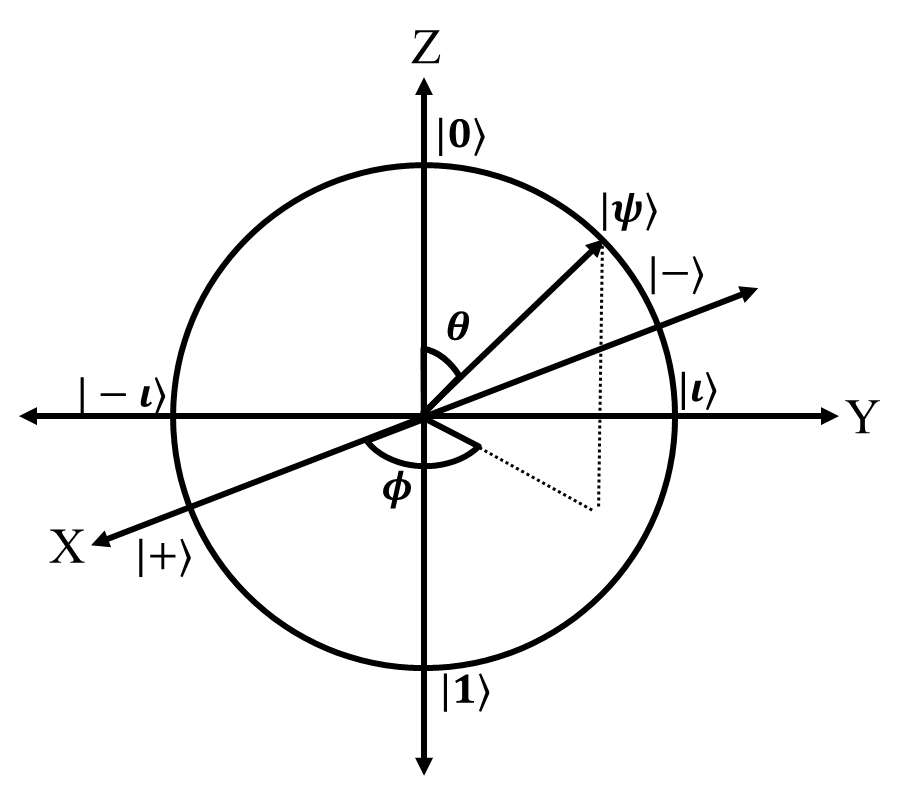
\includegraphics[width=0.6\textwidth]{Images/bloch_sphere_dia.png}
    \caption{Bloch-Poincare Sphere}
    \label{fig:bloch_sphere}
\end{figure}

Thus for different values of $\theta$ and $\phi$ we get different points on the bloch sphere which
represents the different states of a qubit. For a unique mapping from the $\theta$ and $\phi$ to the points on the Bloch Sphere,
we restrict the value of $\theta \in [0,\pi]$ and $\phi \in [0,2\pi]$. 
Thus, the state of a qubit can be represented as:
\[
    \ket{\psi}=\cos\left(\frac{\theta}{2}\right)\ket{0}+e^{\iota \phi}\sin\left(\frac{\theta}{2}\right)\ket{1}
\]
where $\theta \in [0,\pi]$ and $\phi \in [0,2\pi]$ are the polar (represents magnitude or argument) and azimuthal (represents relative phase) angles of the Bloch Sphere respectively.
The following code using Qiskit can be used to plot the Bloch Sphere.
For running the code you need to install the qiskit library. 
%Insert a link 
\href{https://docs.quantum.ibm.com/start/install}{Click here for guide on installing qiskit}
\begin{lstlisting}[language=Python]
import matplotlib.pyplot as plt
from qiskit.visualization import plot_bloch_vector # Import the function to plot the Bloch vector
from qiskit.visualization import plot_bloch_multivector # Import the function to plot the Bloch vector

'''
Function to plot the Bloch Sphere

plot_bloch_vector(bloch, title='', ax=None, figsize=None, coord_type='spherical', font_size=None)

Plots a Bloch Sphere

Parameters
- bloch (list[double]) - array of three elements where [<x>, <y>, <z>] (Cartesian) or 
[<r>, <theta>, <phi>] (spherical in radians) <theta> is inclination angle from +z direction 
<phi> is azimuth from +x direction
- title (str) - a string that represents the title of the plot
- ax (matplotlib.axes.Axes) - an axes of the current figure to plot the Bloch sphere into
- figsize (tuple) - a tuple (width, height) in inches that represents the size of the figure
- coord_type (str) - the coordinate system to use. 'spherical' or 'cartesian', default is cartesian
- font_size (int) - the font size of the tex

Returns
- matplotlib.figure.Figure - a matplotlib figure object

Raises
- ImportError - if matplotlib is not installed
'''

plot_bloch_vector([0,1,0],title='Bloch Sphere')
\end{lstlisting}
The output of the above code is shown in the figure \ref{fig:bloch_sphere_code}.
%Insert a figure
\begin{figure}[ht]
    \centering
    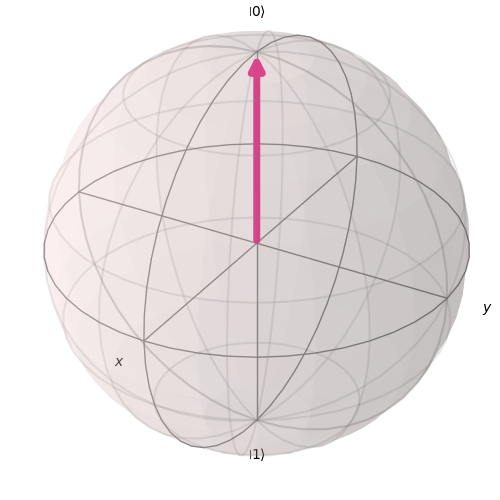
\includegraphics[width=0.5\textwidth]{Images/bloch_sphere.png}
    \caption{Bloch Sphere}
    \label{fig:bloch_sphere_code}
\end{figure}
\textbf{Note that the Bloch Sphere is a geometric representation of the pure states of a qubit. The mixed states of a qubit are represented by the interior of the Bloch Sphere.}

\begin{example}
    The state of a qubit for different values of $\theta$ and $\phi$ is shown in the table \ref{tab:bloch_sphere}.
    \begin{table}[ht]
        \centering
        \begin{tabular}{|c|c|>{\centering\arraybackslash}m{8cm}|c|}
            \hline
            $\theta$ & $\phi$ & State of Qubit & At Axis\\
            \hline
            0 & 0 & $\ket{0}$ & +ve Z\\
            $\pi$ & 0 & $\ket{1}$ & -ve Z \\
            $\frac{\pi}{2}$ & 0 & $\ket{+} = \frac{1}{\sqrt{2}}(\ket{0} + \ket{1})$ & +ve X\\
            $\frac{\pi}{2}$ & $\pi$ & $\ket{-} = \frac{1}{\sqrt{2}}(\ket{0} - \ket{1})$ & -ve X\\
            $\frac{\pi}{2}$ & $\frac{\pi}{2}$ & $\ket{+\iota}=\frac{1}{\sqrt{2}}(\ket{0} + i\ket{1})$ & +ve Y \\
            $\frac{\pi}{2}$ & $-\frac{\pi}{2}$ & $\ket{-\iota}=\frac{1}{\sqrt{2}}(\ket{0} - i\ket{1})$ & -ve Y\\
            \hline
        \end{tabular}
        \caption{State of a Qubit for different values of $\theta$ and $\phi$}
        \label{tab:bloch_sphere}
    \end{table}
\end{example}

\textbf{Quantum Gates acting on Qubits can be thought of as rotations on the Bloch Sphere with some global phase. The global phase is irrelevant to observable quantities and thus does not impact the practical interpretation of the rotation as a transformation on the Bloch sphere. In other words, doing matrix vector multiplication corresponding to rotation action on qubits is the same up to a global phase. A matrix-vector multiplication by a matrix corresponding to some rotation and the vector corresponding to the state of qubit will introduce a global phase shift which can be ignored. Thus, it is easier to imagine this as rotations on bloch sphere where we ignore the global phases implicitly. For example, $R_x(\pi)\ket{0}=-\iota \ket{1}$ using matrix vector multiplication and $R_x(\pi)\ket{0} = \ket{1}$ using the fact that rotations o bloch sphere method but both of them are the same states up to a global phase i.e. $-\iota = e^{\iota 3\pi/2} \times 1$.}
This will be explained further in the later sections.

Note that orthonormal states reside at the ends of the diameter of the Bloch Sphere. 
Let a state $\ket{\psi}$ be represented by a point on the Bloch Sphere. The state $\ket{\psi}$ can be written as:
\[
    \ket{\psi}=\cos\left(\frac{\theta}{2}\right)\ket{0}+e^{\iota \phi}\sin\left(\frac{\theta}{2}\right)\ket{1}
\]
Then the state (say $\ket{\psi'}$) exactly opposite on the Bloch sphere will have the state:
\[
    \ket{\psi'}=\cos\left(\frac{\pi+\theta}{2}\right)\ket{0}+e^{\iota \phi}\sin\left(\frac{\pi+\theta}{2}\right)\ket{1}
\]
Thus, upon simplifying we get:
\[
    \ket{\psi'}=\cos\left(\frac{\pi+\theta}{2}\right)\ket{0}+e^{\iota \phi}\sin\left(\frac{\pi+\theta}{2}\right)\ket{1}
\]
\[
    \ket{\psi'}=-\sin \left(\frac{\theta}{2}\right)\ket{0}+e^{\iota \phi}\cos\left(\frac{\theta}{2}\right)\ket{1}
\]
Now taking the inner product of the states $\ket{\psi}$ and $\ket{\psi'}$ we get:
\[
    \braket{\psi|\psi'}=-\sin\left(\frac{\theta}{2}\right)\cos\left(\frac{\theta}{2}\right)+e^{\iota \phi}e^{-\iota \phi}\sin\left(\frac{\theta}{2}\right)\cos\left(\frac{\theta}{2}\right)=0
\]
Thus, the inner product is zero which implies that the states on the opposite ends of the Bloch Sphere are orthogonal.

\textbf{Note: Such a correspondence does not exist for higher dimensions i.e. No such visualization exists for say Qudits which is d level quantum systems.}
From figure \ref{fig:bloch_sphere} we can see that to convert from polar to cartesian coordinates we use the following relations:
\[
    x=r\sin\theta\cos\phi
\]
\[
    y=r\sin\theta\sin\phi
\]
\[
    z=r\cos\theta
\]
note that here $r=1$ (from pure states i.e. points on the surface of the sphere). To convert from carteisan to polar coordinates we use the following relations:
\[
    r=\sqrt{x^2+y^2+z^2}
\]
\[
    \theta=\cos^{-1}(z)
\]
\[
    \phi=\tan^{-1}\left(\frac{y}{x}\right)
\]
Let us denote the vector as $\vec{n}=(\sin\theta \cos \phi, \sin \theta \sin \phi, \cos \theta, \cos \theta)$.
Points on a Bloch sphere is alwyas a pure state.


\section{Single Qubit Gates}
As said earlier that quantum gates are unitary operators that act on the state of a quantum system. 
Recall from Appendix that the unitary operators are the ones that preserve the inner product of the vectors and the norm of the vectors i.e. they 
only rotate the vectors in the complex vector space (Rotation matrices in $\mathbb{C}^n$). Thus, a state normalized initially remains in the normalized state and does not change its norm 
upon the action of Unitary gates/operators.
The single qubit gates are the quantum gates that act on a single qubit, represented by 2x2 matrices. Since a quantum state is represented by a column vector (in some basis, generally standard basis). 
A gate is a unitary matrix/transformation 
that acts on the qubit(column vector) and changes its state to some other state.
They are rotations on the Bloch Sphere.
\begin{example}
    Consider a $2 \times 2$ matrix $U$ given as:
    \[
        U=\begin{bmatrix}
            a & b \\
            c & d
        \end{bmatrix}
    \]
    in the orthonormal input and output basis $\{\ket{0},\ket{1}\}$, thus, we can write the matrix $U$ as:
    \[
        U=a\ket{0}\bra{0}+b\ket{0}\bra{1}+c\ket{1}\bra{0}+d\ket{1}\bra{1}
    \]
    This, will be used to express the Pauli Matrices in the later sections.
\end{example}

\subsection{Pauli Matrices}
\subsubsection{Pauli-I Gate}
It is used for the measurement of decoherence (Qubits start to lose its Quantum abilities after certain time).
The Truth table is given as in table \ref{tab:pauli-i}. It does no rotation of the bloch vector on the Bloch Sphere.
%Insert a table
\begin{table}[ht]
    \centering
    \begin{tabular}{|c|c|}
        \hline
        Input & Output\\
        \hline  
        $\ket{0}$ & $\ket{0}$\\
        $\ket{1}$ & $\ket{1}$\\
        \hline
    \end{tabular}
    \caption{Truth Table for Pauli-I Gate}
    \label{tab:pauli-i}
\end{table}
The code for the Pauli-I Gate is as follows:
\begin{lstlisting}[language=Python]
from qiskit import QuantumRegister, ClassicalRegister, QuantumCircuit
from numpy import pi

qreg_q = QuantumRegister(1, 'q')

circuit = QuantumCircuit(qreg_q)

circuit.id(qreg_q[0]) #For Pauli-Identity Gate
circuit.draw(output='mpl')#.savefig('../images/pauli-i.png') #Draw the circuit
\end{lstlisting}
The circuit symbol is as shown in figure \ref{fig:pauli-i}
\begin{figure}[ht]
    \centering
    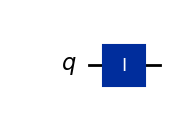
\includegraphics[width=0.3\textwidth]{Images/pauli-i.png}
    \caption{Pauli-I Gate}
    \label{fig:pauli-i}
\end{figure}
In operator Notation it is:
\begin{align*}
    I\ket{0}&=\ket{0} \\
    I\ket{1}&=\ket{1}
\end{align*}
It is represented by the matrix in the computational basis ($\ket{0},\ket{1}$) as:
\[
    \sigma_I=I=\begin{bmatrix}
        1 & 0 \\
        0 & 1
    \end{bmatrix}
\]
It's Eigen values are 1 and 1. It's Eigen vectors are any vector in the 2-D Space.
Note that it's Unitary($II^{\dagger}=I^{\dagger}I=I;I=I^{-1}$) and Hermitian Matrix($I=I^{\dagger}$), thus a Normal Matrix ($II^{\dagger}=I^{\dagger}I$) hence Unitarily digonalizable.
Thus, it has a Spectral decomposition (outer product representation) which can be written as:
\[
    I=\ket{0}\bra{0}+\ket{1}\bra{1}
\]
Action of Pauli-I Gate on a general qubit $\alpha\ket{0}+\beta\ket{1}$ is:
\[
    \begin{bmatrix}
        1 & 0 \\
        0 & 1
    \end{bmatrix}\begin{bmatrix}
        \alpha \\
        \beta
    \end{bmatrix}=\begin{bmatrix}
        \alpha \\
        \beta
    \end{bmatrix}= \alpha\ket{0}+\beta\ket{1}
\]

\subsubsection{Pauli-X Gate}
It is also known as the NOT gate. It is equivalent of Classical NOT Gate.
It is thus called Bit Flip Gate. The truth table is as in \ref{tab:pauli-x}. It does anticlockwise $\pi$ rotation about X 
axis of Bloch sphere. It flips the state $\ket{0}$ to $\ket{1}$ and $\ket{1}$ to $\ket{0}$.
\begin{table}[ht]
    \centering
    \begin{tabular}{|c|c|}
        \hline
        Input & Output\\
        \hline
        $\ket{0}$ & $\ket{1}$\\
        $\ket{1}$ & $\ket{0}$\\
        \hline
    \end{tabular}
    \caption{Truth Table for Pauli-X Gate}
    \label{tab:pauli-x}
\end{table}

The code for the Pauli-X Gate is as follows:
\begin{lstlisting}[language=Python]
from qiskit import QuantumRegister, ClassicalRegister, QuantumCircuit
from numpy import pi

qreg_q = QuantumRegister(1, 'q')
circuit = QuantumCircuit(qreg_q,name='Not Gate')

circuit.x(qreg_q[0])

circuit.draw(output='mpl')#.savefig('../images/pauli-x.png') #Draw the circuit
\end{lstlisting}
The circuit symbol is as shown in figure \ref{fig:pauli-x}.
\begin{figure}[ht]
    \centering
    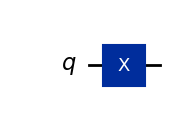
\includegraphics[width=0.3\textwidth]{Images/pauli-x.png}
    \caption{Pauli-X Gate}
    \label{fig:pauli-x}
\end{figure}
In the operator Notation it is:
\begin{align*}
    X\ket{0}&=\ket{1} \\
    X\ket{1}&=\ket{0}
\end{align*}
It is represented by the matrix in the computational basis ($\ket{0},\ket{1}$) as:
\[
    \sigma_X=X=\begin{bmatrix}
        0 & 1 \\
        1 & 0
    \end{bmatrix}
\]
It's Eigen values are 1 and -1. It's corresponding Eigen vectors are $\ket{+}=\frac{1}{\sqrt{2}}(\ket{0}+\ket{1})$ and $\ket{-}=\frac{1}{\sqrt{2}}(\ket{0}-\ket{1})$.
It is a Unitary and Hermitian Matrix. It is a Normal Matrix hence Unitarily Diagonalizable.
It has a Spectral decomposition (outer product representation) which can be written as:
\[
    X=\ket{+}\bra{+}-\ket{-}\bra{-}
\]
Upon, substituting the values of $\ket{+}$ and $\ket{-}$ we get:
\begin{align*}
    X&=\dfrac{1}{\sqrt{2}}(\ket{0}+\ket{1})\dfrac{1}{\sqrt{2}}(\bra{0}+\bra{1})-\dfrac{1}{\sqrt{2}}(\ket{0}-\ket{1})\dfrac{1}{\sqrt{2}}(\bra{0}-\bra{1})\\
    &=\dfrac{1}{2}(\ket{0}\bra{0}+\ket{0}\bra{1}+\ket{1}\bra{0}+\ket{1}\bra{1})-\dfrac{1}{2}(\ket{0}\bra{0}-\ket{0}\bra{1}-\ket{1}\bra{0}+\ket{1}\bra{1})\\
    &=\ket{0}\bra{1}+\ket{1}\bra{0}
\end{align*}
Thus, the Pauli-X Gate can also be written as:
\[
    X=\ket{0}\bra{1}+\ket{1}\bra{0}
\]
\textbf{Note that the Pauli-X Gate can be written as $X=HZH$ or $\sigma_X=H\sigma_Z H$  where $H$ and $Z$ are the Hadamard and Pauli-Z Gates respectively.}
Action of Pauli-X Gate on a general qubit $\ket{\psi}=\alpha\ket{0}+\beta\ket{1}$ is: 
\[
    \begin{bmatrix}
        0 & 1 \\
        1 & 0
    \end{bmatrix}\begin{bmatrix}
        \alpha \\
        \beta
    \end{bmatrix}=\begin{bmatrix}
        \beta \\
        \alpha
    \end{bmatrix}= \beta\ket{0}+\alpha\ket{1}
\]

\subsubsection{Pauli-Y Gate}
It is a anitclockwise $\pi$ rotation about Y axis of Bloch Sphere. 
It flips the Qubit and muultiplies a complex amplitude. The truth table is as in table \ref{tab:pauli-y}.
\begin{table}[ht]
    \centering
    \begin{tabular}{|c|c|}
        \hline
        Input & Output\\
        \hline
        $\ket{0}$ & $i\ket{1}$\\
        $\ket{1}$ & $-i\ket{0}$\\
        \hline
    \end{tabular}
    \caption{Truth Table for Pauli-Y Gate}
    \label{tab:pauli-y}
\end{table}
The code for the Pauli-Y Gate is as follows:
\begin{lstlisting}[language=Python]
from qiskit import QuantumRegister, ClassicalRegister, QuantumCircuit
from numpy import pi

qreg_q = QuantumRegister(1, 'q')
circuit = QuantumCircuit(qreg_q,name='Not Gate')

circuit.y(qreg_q[0]) #Apply the Y gate

circuit.draw(output='mpl')#.savefig('../images/pauli-x.png') #Draw the circuit
\end{lstlisting}

The circuit symbol is as shown in figure \ref{fig:pauli-y}.
\begin{figure}[ht]
    \centering
    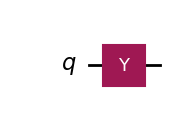
\includegraphics[width=0.3\textwidth]{Images/pauli-y.png}
    \caption{Pauli-Y Gate}
    \label{fig:pauli-y}
\end{figure}
In the operator Notation it is:
\begin{align*}
    Y\ket{0}&=i\ket{1} \\
    Y\ket{1}&=-i\ket{0}
\end{align*}
It is represented by the matrix in the computational basis ($\ket{0},\ket{1}$) as:
\[
    \sigma_Y=Y=\begin{bmatrix}
        0 & -i \\
        i & 0
    \end{bmatrix}
\]
It's Eigen values are 1 and -1. It's corresponding Eigen vectors are $\ket{+i}=\frac{1}{\sqrt{2}}(\ket{0}+i\ket{1})$ and $\ket{-i}=\frac{1}{\sqrt{2}}(\ket{0}-i\ket{1})$.
It is a Unitary and Hermitian Matrix. It is a Normal Matrix hence Unitarily Diagonalizable.
It has a Spectral decomposition (outer product representation) which can be written as:
\[
    Y=\ket{+i}\bra{+i}-\ket{-i}\bra{-i}
\]
Upon, substituting the values of $\ket{+i}$ and $\ket{-i}$ we get:
\begin{align*}
    Y&=\dfrac{1}{\sqrt{2}}(\ket{0}+i\ket{1})\dfrac{1}{\sqrt{2}}(\bra{0}-i\bra{1})-\dfrac{1}{\sqrt{2}}(\ket{0}-i\ket{1})\dfrac{1}{\sqrt{2}}(\bra{0}+i\bra{1})\\
    &=\dfrac{1}{2}(\ket{0}\bra{0}-i\ket{0}\bra{1}+i\ket{1}\bra{0}+\ket{1}\bra{1})-\dfrac{1}{2}(\ket{0}\bra{0}+i\ket{0}\bra{1}-i\ket{1}\bra{0}+\ket{1}\bra{1})\\
    &=i\ket{1}\bra{0}-i\ket{0}\bra{1}
\end{align*}
Thus, the Pauli-Y Gate can also be written as:
\[
    Y=-i\ket{0}\bra{1}+i\ket{1}\bra{0}
\]
\textbf{Note that the Pauli-Y Gate can be written as $Y=\iota XZ$ or $\sigma_Y=\iota \sigma_X\sigma_Z$  where $X$ and $Z$ are the Pauli-X and Pauli-Z Gates respectively.}
This means that the Pauli-Y Gate is a rotation about the Y-axis of the Bloch Sphere by $\pi$ in anticlocwise direction and is equivalent to a rotation about the X-axis by anticlockwise $\pi$ followed by a rotation about the Z-axis by anticlockwise $\pi$
(upto a global phase).

Action of Pauli-Y Gate on a general qubit $\ket{\psi}=\alpha\ket{0}+\beta\ket{1}$ is:
\[
    \begin{bmatrix}
        0 & -i \\
        i & 0
    \end{bmatrix}\begin{bmatrix}
        \alpha \\
        \beta
    \end{bmatrix}=\begin{bmatrix}
        -i\beta \\
        i\alpha
    \end{bmatrix}=i\alpha\ket{1}-i\beta\ket{0}
\]

\subsubsection{Pauli-Z Gate}
It is a anticlockwise $\pi$ rotation about Z axis of Bloch Sphere.
It flips the sign of the $\ket{1}$ state. It is also called Phase Flip/Phase shoft/Sign flip gate.
The truth table is as in table \ref{tab:pauli-z}.
\begin{table}[ht]
    \centering
    \begin{tabular}{|c|c|}
        \hline
        Input & Output\\
        \hline
        $\ket{0}$ & $\ket{0}$\\
        $\ket{1}$ & $-\ket{1}$\\
        \hline
    \end{tabular}
    \caption{Truth Table for Pauli-Z Gate}
    \label{tab:pauli-z}
\end{table}
The code for the Pauli-Z Gate is as follows:
\begin{lstlisting}[language=Python]
from qiskit import QuantumRegister, ClassicalRegister, QuantumCircuit
from numpy import pi

qreg_q = QuantumRegister(1, 'q')
circuit = QuantumCircuit(qreg_q,name='Not Gate')

circuit.z(qreg_q[0]) #Apply the Z gate

circuit.draw(output='mpl')#.savefig('../images/pauli-z.png') #Draw the circuit
\end{lstlisting}
The circuit symbol is as shown in figure \ref{fig:pauli-z}.
\begin{figure}[ht]
    \centering
    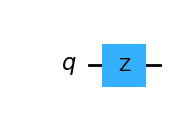
\includegraphics[width=0.3\textwidth]{Images/pauli-z.png}
    \caption{Pauli-Z Gate}
    \label{fig:pauli-z}
\end{figure}
In the operator Notation it is:
\begin{align*}
    Z\ket{0}&=\ket{0} \\
    Z\ket{1}&=-\ket{1}
\end{align*}
It is represented by the matrix in the computational basis ($\ket{0},\ket{1}$) as:
\[
    \sigma_Z=Z=\begin{bmatrix}
        1 & 0 \\
        0 & -1
    \end{bmatrix}
\]
It's Eigen values are 1 and -1. It's corresponding Eigen vectors are $\ket{0}$ and $\ket{1}$.
It is a Unitary and Hermitian Matrix. It is a Normal Matrix hence Unitarily Diagonalizable.
It has a Spectral decomposition (outer product representation) which can be written as:
\[
    Z=\ket{0}\bra{0}-\ket{1}\bra{1}
\]
In Compact form, we can write Pauli-Z Gate as:
\[
    Z\ket{j}=(-1)^j\ket{j}
\]
where $j=0,1$.
Action of Pauli-Z Gate on a general qubit $\ket{\psi}=\alpha\ket{0}+\beta\ket{1}$ is:
\[
    \begin{bmatrix}
        1 & 0 \\
        0 & -1
    \end{bmatrix}\begin{bmatrix}
        \alpha \\
        \beta
    \end{bmatrix}=\begin{bmatrix}
        \alpha \\
        -\beta
    \end{bmatrix}=\alpha\ket{0}-\beta\ket{1}
\]
\begin{example}
    \textbf{(Pauli Matrices: Hermitian and Unitary)} Show that the pauli matrices are Hermitian and unitary.

    We check $I,X,Y,Z$ in turns.
    \[
    I^{\dagger}=\left(\begin{bmatrix} 1 & 0 \\ 0 & 1 \end{bmatrix}^T \right)^* = \begin{bmatrix} 1 & 0 \\ 0 & 1 \end{bmatrix}^* = \begin{bmatrix} 1 & 0 \\ 0 & 1 \end{bmatrix} =I
    \]
    \[
    I^{\dagger}I=II=I
    \]
    \[
    X^{\dagger}=\left(\begin{bmatrix} 0 & 1 \\ 1 & 0 \end{bmatrix}^T \right)^* = \begin{bmatrix} 0 & 1 \\ 1 & 0 \end{bmatrix}^* = \begin{bmatrix} 0 & 1 \\ 1 & 0 \end{bmatrix} =X
    \]
    \[
    X^{\dagger}X=XX=\begin{bmatrix} 0 & 1 \\ 1 & 0 \end{bmatrix} = \begin{bmatrix} 0 & 1 \\ 0 & 1 \end{bmatrix} = I
    \]
    \[
    Y^{\dagger}=\left(\begin{bmatrix} 0 & -\iota \\ \iota & 0 \end{bmatrix}^T \right)^* = \begin{bmatrix} 0 & \iota \\ -\iota & 0 \end{bmatrix}^* = \begin{bmatrix} 0 & -\iota \\ \iota & 0 \end{bmatrix} =Y
    \]
    \[
    Y^{\dagger}Y=YY=\begin{bmatrix} 0 & -\iota \\ \iota & 0 \end{bmatrix} \begin{bmatrix} 0 & -\iota \\ \iota & 0 \end{bmatrix}=\begin{bmatrix} 1 & 0 \\ 0 & 1 \end{bmatrix}
     \]
    \[
    Z^{\dagger}=\left(\begin{bmatrix} 1 & 0 \\ 0 & -1 \end{bmatrix}^T \right)^* = \begin{bmatrix} 1 & 0 \\ 0 & -1 \end{bmatrix}^* = \begin{bmatrix} 1 & 0 \\ 0 & -1 \end{bmatrix} =Z
    \]
    \[
    Z^{\dagger}Z=\begin{bmatrix} 1 & 0 \\ 0 & -1 \end{bmatrix} \begin{bmatrix} 1 & 0 \\ 0 & -1 \end{bmatrix} = \begin{bmatrix} 1 & 0 \\ 0 & 1 \end{bmatrix} = I
    \]
\end{example}

\begin{example}
    Calculate the matrix representation of the tensor products of the Pauli operators (a)$X$ and $Z$; (b)$I$ and $X$; (c) $X$ and $I$. Is the tensor product commutative?

    Using Kronecker product we have,
    \begin{enumerate}
        \item 
        \[
        X\otimes Z=\begin{bmatrix}
            0Z & 1Z \\ 1Z & 0Z
        \end{bmatrix}= \begin{bmatrix}
            0\begin{bmatrix} 1 & 0 \\ 0 & -1 \end{bmatrix} & 1 \begin{bmatrix} 1 & 0 \\ 0 & -1 \end{bmatrix} \\ 1 \begin{bmatrix} 1 & 0 \\ 0 & -1 \end{bmatrix} & 0 \begin{bmatrix} 1 & 0 \\ 0 & -1 \end{bmatrix}
        \end{bmatrix}=\begin{bmatrix} 0 & 0 & 1 & 0 \\ 0 & 0 & 0 -1 \\ 1 & 0 & 0 & 0 \\ 0 & -1 & 0 & 0 \end{bmatrix}
        \]
        \item
        \[
        I\otimes X=\begin{bmatrix}
            1X & 0X \\ 0X & 1X
        \end{bmatrix}= \begin{bmatrix}
            1\begin{bmatrix} 0 & 1 \\ 1 & 0 \end{bmatrix} & 0 \begin{bmatrix} 0 & 1 \\ 1 & 0 \end{bmatrix} \\ 0 \begin{bmatrix} 0 & 1 \\ 1 & 0 \end{bmatrix} & 1 \begin{bmatrix} 0 & 1 \\ 1 & 0 \end{bmatrix}
        \end{bmatrix}=\begin{bmatrix} 0 & 1 & 0 & 0 \\ 1 & 0 & 0 & 0 \\ 0 & 0 & 0 & 1 \\ 0 & 0 & 1 & 0 \end{bmatrix}
        \]
        \item 
        \[
        X\otimes I=\begin{bmatrix}
            0I & 1I \\ 1I & 0I
        \end{bmatrix}= \begin{bmatrix}
            0\begin{bmatrix} 1 & 0 \\ 0 & 1 \end{bmatrix} & 1\begin{bmatrix} 1 & 0 \\ 0 & 1 \end{bmatrix} \\ 1\begin{bmatrix} 1 & 0 \\ 0 & 1 \end{bmatrix} & 0\begin{bmatrix} 1 & 0 \\ 0 & 1 \end{bmatrix}
        \end{bmatrix}=\begin{bmatrix} 0 & 0 & 1 & 0 \\ 0 & 0 & 0 & 1 \\ 1 & 0 & 0 & 0 \\ 0 & 1 & 0 & 0 \end{bmatrix}
        \]
    \end{enumerate}
    Comparing (b) and (c), we conclude and adjoint operations distribute over the tensor product.
\end{example}

\begin{example}
    \textbf{(Commutation relations for the Pauli Matrices)} Verify the commutation relations
    \[
    [X,Y]=2\iota Z;[Y,Z]=2\iota X;[Z,X]=2\iota Y
    \]
    There is an elegant way of writing this using $\epsilon_{jkl}$, the antisymmetric tensor on three indices, for which $\epsilon_{jkl}=0$ except for $\epsilon_{123}=\epsilon_{231}=\epsilon_{312}=1$, and $\epsilon_{321}=\epsilon_{213}=\epsilon_{132}=-1$:
    \[
    [\sigma_j,\sigma_k]=2\iota\sum_{l=1}^3 \epsilon_{jkl}\sigma_l
    \]

    We verify the proposed relations via computation in the computational basis:
    \[
    [X,Y]=XY-YX=\begin{bmatrix} 0 & 1 \\ 1 & 0 \end{bmatrix}\begin{bmatrix} 0 & -\iota \\ \iota & 0 \end{bmatrix} - \begin{bmatrix}0 & -\iota \\ \iota & 0 \end{bmatrix} \begin{bmatrix} 0 & 1 \\ 1 & 0 \end{bmatrix} = \begin{bmatrix} \iota & 0 \\ 0 & -\iota \end{bmatrix} - \begin{bmatrix} -\iota & 0 \\ 0 & \iota \end{bmatrix} =2\iota Z
    \]
    \[
    [Y,Z]=YZ-ZY=\begin{bmatrix} 0 & -\iota  \\ \iota & 0 \end{bmatrix}\begin{bmatrix} 1 & 0 \\ 0 & -1 \end{bmatrix} - \begin{bmatrix} 1 & 0 \\ 0 & -1 \end{bmatrix} \begin{bmatrix} 0 & -\iota  \\ \iota & 0 \end{bmatrix} = \begin{bmatrix} 0 & \iota \\ \iota & 0 \end{bmatrix} - \begin{bmatrix} 0 & -\iota \\ -\iota & 0 \end{bmatrix} =2\iota X
    \]
    \[
    [Z,X]=ZX-XZ=\begin{bmatrix} 1 & 0 \\ 0 & -1 \end{bmatrix}\begin{bmatrix} 0 & 1 \\ 1 & 0 \end{bmatrix} - \begin{bmatrix}0 & 1 \\ 1 & 0 \end{bmatrix} \begin{bmatrix} 1 & 0 \\ 0 & -1 \end{bmatrix} = \begin{bmatrix} 0 & 1 \\ -1 & 0 \end{bmatrix} - \begin{bmatrix} 0 & -1 \\ 1 & 0 \end{bmatrix} =2\iota Y
    \]
\end{example}
\begin{example}
    \textbf{(Anti-commutation relations for the Pauli matrices)} Verify the anti-communal relations
    \[
    \{\sigma_i,\sigma_j\}=0
    \]
    where $i\neq j$ are both chosen from the set $1,2,3$. Also verify that $(i=0,1,2,3)$
    \[
    \sigma_i^2=I
    \]
    We again verify the proposed relations via computation in the computational basis:
    \[
    \{X,Y\}=XY+YX=\begin{bmatrix} 0 & 1 \\ 1 & 0 \end{bmatrix}\begin{bmatrix} 0 & -\iota  \\ \iota & 0 \end{bmatrix}+\begin{bmatrix} 0 & -\iota  \\ \iota & 0 \end{bmatrix}\begin{bmatrix} 0 & 1 \\ 1 & 0 \end{bmatrix}=\begin{bmatrix} \iota & 0 \\ 0 & -\iota \end{bmatrix}+\begin{bmatrix} -\iota & 0 \\ 0 & \iota \end{bmatrix} = \begin{bmatrix} 0 & 0 \\ 0 & 0 \end{bmatrix}
    \]
    \[
    \{Y,Z\}=YZ+ZY=\begin{bmatrix} 0 & -\iota  \\ \iota & 0 \end{bmatrix}\begin{bmatrix} 1 & 0 \\ 0 & -1 \end{bmatrix}+\begin{bmatrix} 1 & 0 \\ 0 & -1 \end{bmatrix}\begin{bmatrix} 0 & -\iota  \\ \iota & 0 \end{bmatrix}=\begin{bmatrix} 0 & \iota \\ \iota & 0 \end{bmatrix}+\begin{bmatrix} 0 & -\iota \\ -\iota & 0 \end{bmatrix} = \begin{bmatrix} 0 & 0 \\ 0 & 0 \end{bmatrix}
    \]
    \[
    \{Z,X\}=ZX+XZ=\begin{bmatrix} 1 & 0 \\ 0 & -1 \end{bmatrix}\begin{bmatrix} 0 & 1 \\ 1 & 0 \end{bmatrix}+\begin{bmatrix} 0 & 1 \\ 1 & 0 \end{bmatrix}\begin{bmatrix} 1 & 0 \\ 0 & -1 \end{bmatrix}=\begin{bmatrix} 0 & 1 \\ -1 & 0 \end{bmatrix}+\begin{bmatrix} 0 & -1 \\ 1 & 0 \end{bmatrix} = \begin{bmatrix} 0 & 0 \\ 0 & 0 \end{bmatrix}
    \]
    This proves the first claim as $\{A,B\}=AB+BA=BA+AB=\{B,A\}$ and the other 3 relations are equivalent to the ones already proven. Verifying the second claim, we have:
    \[
    I^2=\begin{bmatrix} 1 & 0 \\ 0 & 1\end{bmatrix}\begin{bmatrix} 1 & 0 \\ 0 & 1\end{bmatrix}=\begin{bmatrix} 1 & 0 \\ 0 & 1\end{bmatrix}=I
    \]
    \[
    X^2=\begin{bmatrix} 0 & 1 \\ 1 & 0 \end{bmatrix}\begin{bmatrix} 0 & 1 \\ 1 & 0 \end{bmatrix}=\begin{bmatrix} 0 & 1 \\ 1 & 0 \end{bmatrix}=I
    \]
    \[
    Y^2=\begin{bmatrix} 0 & -\iota \\ \iota & 0 \end{bmatrix}\begin{bmatrix} 0 & -\iota \\ \iota & 0 \end{bmatrix}=\begin{bmatrix} 0 & -\iota \\ \iota & 0 \end{bmatrix}=I
    \]
    \[
    Z^2=\begin{bmatrix} 1 & 0 \\ 0 & -1 \end{bmatrix}\begin{bmatrix} 1 & 0 \\ 0 & -1 \end{bmatrix}=\begin{bmatrix} 1 & 0 \\ 0 & -1 \end{bmatrix}=I
    \]
    \begin{remark}
        Note that we can write this result concisely as $\{\sigma_j,\sigma_k\}=2\delta_{jk}I$
    \end{remark}
\end{example}
\begin{example}
    Show that for $j=1,2,3$
    \[
    \sigma_j\sigma_k=\delta_{jk} I + \iota \sum_{l=1}^3 \epsilon_{jkl}\sigma_l
    \]
    Applying the previous results we get,
    \begin{align*}
    \sigma_j\sigma_k&=\frac{[\sigma_j,\sigma_k]+\{\sigma_j,\sigma_k\}}{2}\\
    &=\frac{2\iota \sum_{l=1}^3 \epsilon_{jkl}\sigma_l +2\delta_{ij}I}{2}\\
    &=\delta_{jk}I+\iota\sum_{l=1}^3 \epsilon_{jkl}\sigma_l
    \end{align*}
\end{example}
\begin{importantnote}
Note that all the Pauli-gate are Unitary and Hermitian. Since, all the Unitary gates ($U^{\dagger}=U^{-1}$)
are reversible. Thus, from Postulate 2: Evolution, we can apply Pauli Gates. All the Pauli gates are reversible 
and thus can be applied in Quantum Circuits. The four Pauli gates can also be denoted as $X=\sigma_X$, $Y=\sigma_Y$, $Z=\sigma_Z$ and $I=\sigma_I$.
All the Pauli Gates as said earlier are anticlockwise rotations on the Bloch Sphere. The Pauli-X Gate is a $\pi$ rotation about the X-axis,
Pauli-Y Gate is a $\pi$ rotation about the Y-axis and Pauli-Z Gate is a $\pi$ rotation about the Z-axis. The Pauli-I Gate does not do any rotation on the Bloch Sphere.
Also note that applyin the same gate twice will be equivalent to applying the Identity Gate. Thus, the Pauli Gates are self-inverse. Since they are hermitian hence, $U^{\dagger}=U$ and 
they are unitary thus, $U^{\dagger}U=UU^{\dagger}=I$. Thus combining, the two we get $U^2=I$.
This, can also be verified as shown below:
\[
    X^2=\begin{bmatrix}
        0 & 1 \\
        1 & 0
    \end{bmatrix}\begin{bmatrix}
        0 & 1 \\
        1 & 0
    \end{bmatrix}=\begin{bmatrix}
        1 & 0 \\
        0 & 1
    \end{bmatrix}=I
\]
\[
    Y^2=\begin{bmatrix}
        0 & -i \\
        i & 0
    \end{bmatrix}\begin{bmatrix}
        0 & -i \\
        i & 0
    \end{bmatrix}=\begin{bmatrix}
        1 & 0 \\
        0 & 1
    \end{bmatrix}=I
\]
\[
    Z^2=\begin{bmatrix}
        1 & 0 \\
        0 & -1
    \end{bmatrix}\begin{bmatrix}
        1 & 0 \\
        0 & -1
    \end{bmatrix}=\begin{bmatrix}
        1 & 0 \\
        0 & 1
    \end{bmatrix}=I
\]
\[
    I^2=\begin{bmatrix}
        1 & 0 \\
        0 & 1
    \end{bmatrix}\begin{bmatrix}
        1 & 0 \\
        0 & 1
    \end{bmatrix}=\begin{bmatrix}
        1 & 0 \\
        0 & 1
    \end{bmatrix}=I
\]
Thus, we can see that all the Pauli Gates are self-inverse.
The Pauli gates also form the basis for the single qubit gates. Any single qubit gate can be written as a linear combination of the Pauli Gates.
In other words, any $2 \times 2$ matrix can be written as a linear combination of the Pauli Matrices.
\[
    A=\alpha I+\beta X+\gamma Y+\delta Z
\]
where $\alpha,\beta,\gamma,\delta$ are complex numbers. The Pauli Matrices, except Identity are also traceless (trace=0) as can be clearly inferred from the matrices and all the Pauli matrices are Hermitian.
Note here it should be presumed that the the rotations are always in anticlockwise direction.
\end{importantnote}
\begin{example}
    \textbf{(Pauli operators and the outer product)} The Pauli matrices can be considered as operators with respect to an orthonormal basis $\ket{0},\ket{1}$ for a two-dimensional Hilbert space. Express each of the Pauli operators in the outer product notation
    
    Recall that if $A$ has matrix representation
    \[
    A=\begin{bmatrix} a_{00} & a_{01} \\ a_{10} & a_{11} \end{bmatrix}
    \]
    with respect to $\ket{0},\ket{1}$ as the input/output bases, then we can express $A$ in outer product notation as:
    \[
    A=a_{00}\ket{0}\bra{0} + a_{01}\ket{0}\bra{1} + a_{10}\ket{1}\bra{0} + a_{11}\ket{1}\bra{1}
    \]
    Furthermore, recall the representation of Pauli matrices with respect to the orthonormal basis $ket{0},\ket{1}:$
    \[
    I=\begin{bmatrix} 1 & 0 \\ 0 & 1 \end{bmatrix}\quad X=\begin{bmatrix} 0 & 1 \\ 1 & 0 \end{bmatrix} \quad Y=\begin{bmatrix} 0 & -\iota \\ \iota & 0 \end{bmatrix} \quad Z=\begin{bmatrix} 1 & 0 \\ 0 & -1 \end{bmatrix}
    \]
    We immediately see that:
    \begin{align*}
        I&=\ket{0}\bra{0}+\ket{1}\bra{1}\\
        X&=\ket{0}\bra{1}+\ket{1}\bra{0}\\
        Y&=-\iota \ket{0}\bra{1} + \iota \ket{1}\bra{0}\\
        Z&=\ket{0}\bra{0}-\ket{1}\bra{1}
    \end{align*}
\end{example}

\begin{example}
    \textbf{(Eigendecomposition of the Pauli matrices)}
    Find the eigenvectors, eigenvalues and diagonal representation of the Pauli matrices I,X,Y and Z.
    The eigenvectors and eigenvalues of I are the entire space $\mathbb{C}^2$ and $\lambda=1,1$ respectively and its diagonal representation is 
    \[
    I=\ket{0}\bra{0}+\ket{1}\bra{1}
    \]
    Recall that the eigenvectors, eigenvalues of X are $\ket{+},\ket{-}$ and $\lambda=1,-1$ respectively. The diagonal representation will be,
    \[
    X=\ket{+}\bra{+}-\ket{-}\bra{-}
    \]
    Similarly, the eigenvectors and eigenvalue of $Y$ are $\lambda=1,-1$ and $\ket{+\iota},\ket{-\iota}$ respectively, and its diagonal representation is
    \[
    Y=\ket{+\iota}\bra{+\iota}-\ket{-\iota}\bra{-\iota}
    \]
    Similarly, the eigenvectors and eigenvalues of $Z$ are $\lambda=1,-1$ and $\ket{0},\ket{1}$ respectively, and its diagonal representation is
    \[
    Z=\ket{0}\bra{0}-\ket{1}\bra{1}
    \]
\end{example}
\subsection{Hadamard Gate}\label{qgate:hadamard}
It creates a superposition of Qubits. 
It is a $\pi$ rotation about the X+Z axis of Bloch Sphere or 
a $\pi/2$ rotation about the Y axis followed by a $\pi$ rotation about the X axis.
The truth table is as in table \ref{tab:hadamard}.
\begin{table}[ht]
    \centering
    \begin{tabular}{|c|c|}
        \hline
        Input & Output\\
        \hline
        $\ket{0}$ & $\ket{+}=\frac{1}{\sqrt{2}}(\ket{0}+\ket{1})$\\
        $\ket{1}$ & $\ket{-}=\frac{1}{\sqrt{2}}(\ket{0}-\ket{1})$\\
        \hline
    \end{tabular}
    \caption{Truth Table for Hadamard Gate}
    \label{tab:hadamard}
\end{table}

The code for the Hadamard Gate is as follows:
\begin{lstlisting}[language=Python]
from qiskit import QuantumRegister, ClassicalRegister, QuantumCircuit
from numpy import pi

qreg_q = QuantumRegister(1, 'q')
circuit = QuantumCircuit(qreg_q,name='Hadamard Gate')

circuit.h(qreg_q[0]) #Apply the H gate

circuit.draw(output='mpl')#.savefig('../images/hadamard.png') #Draw the circuit
\end{lstlisting}

The circuit symbol is as shown in figure \ref{fig:hadamard}.
\begin{figure}[ht]
    \centering
    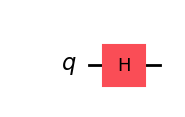
\includegraphics[width=0.3\textwidth]{Images/hadamard.png}
    \caption{Hadamard Gate}
    \label{fig:hadamard}
\end{figure}
In the operator Notation it is:
\begin{align*}
    H\ket{0}&=\dfrac{1}{\sqrt{2}}(\ket{0}+\ket{1})=\ket{+} \\
    H\ket{1}&=\dfrac{1}{\sqrt{2}}(\ket{0}-\ket{1})=\ket{-}
\end{align*}
Generally in a quantum circuit we intialise a qubit in state $\ket{0}$ and thus Hadamard gate can be used
to create a superposition. It is represented by the matrix in the computational basis ($\ket{0},\ket{1}$) as:
\[
    H=\dfrac{1}{\sqrt{2}}\begin{bmatrix}
        1 & 1 \\
        1 & -1
    \end{bmatrix}
\]
In compact form we can write the action of Hadamard Gate on one qubit as:
\[
    H\ket{j}=\dfrac{1}{\sqrt{2}}\sum_{k=0}^{1}(-1)^{jk}\ket{k}
\]
where $j=0,1$.
It is a Unitary and Hermitian Matrix. It is a Normal Matrix hence Unitarily Diagonalizable. It has eigenvalues, $\lambda_1=1,\lambda_2=-1$ and the corresponding normalized eigenvectors are $\frac{1}{\sqrt{2+\sqrt{2}}}\begin{bmatrix} 1+\frac{1}{\sqrt{2}} \\ \frac{1}{\sqrt{2}}\end{bmatrix}$ and $\frac{1}{\sqrt{2-\sqrt{2}}}\begin{bmatrix} -1 + \frac{1}{\sqrt{2}} \\ \frac{1}{\sqrt{2}}\end{bmatrix}$ respectively.
It has a Spectral decomposition (outer product representation) which can be written as:
\[
    H=\ket{+}\bra{0}+\ket{-}\bra{1}
\]
Action of Hadamard Gate on a general qubit $\ket{\psi}=\alpha\ket{0}+\beta\ket{1}$ is:
\[
    \dfrac{1}{\sqrt{2}}\begin{bmatrix}
        1 & 1 \\
        1 & -1
    \end{bmatrix}\begin{bmatrix}
        \alpha \\
        \beta
    \end{bmatrix}=\begin{bmatrix}
        \dfrac{\alpha+\beta}{\sqrt{2}} \\
        \dfrac{\alpha-\beta}{\sqrt{2}}
    \end{bmatrix}=\dfrac{\alpha+\beta}{\sqrt{2}}\ket{0}+\dfrac{\alpha-\beta}{\sqrt{2}}\ket{1}
\]
Note that we cal also write the Hadamard gate as 
\[
H=\frac{X+Z}{\sqrt{2}}=\frac{1}{\sqrt{2}}\left(\begin{bmatrix} 0 & 1 \\ 1 & 0 \end{bmatrix}+\begin{bmatrix} 1 & 0 \\ 0& -1 \end{bmatrix} \right)=\frac{1}{\sqrt{2}}\begin{bmatrix} 1 & 1 \\ 1 & -1 \end{bmatrix}
\]
Note that the Hadamard gate is also a self-inverse gate. Since its Hermitian as well as Unitary, thus $H^{\dagger}=H$ and $H^{\dagger}H=HH^{\dagger}=I; H=H^{-1}$.
Thus, $H^2=I$. Intuitively this means that applying Hadamard gate twice will bring the quantum state back to the same quantum state. This can also be imagined 
as doing rotations on bloch sphere and then arriving back at the same state.
\[ H^2=\dfrac{1}{\sqrt{2}}\begin{bmatrix}
    1 & 1 \\
    1 & -1
\end{bmatrix}\dfrac{1}{\sqrt{2}}\begin{bmatrix}
    1 & 1 \\
    1 & -1
\end{bmatrix}=\dfrac{1}{2}\begin{bmatrix}
    1+1 & 1-1 \\
    1-1 & 1+1
\end{bmatrix}=\begin{bmatrix}
    1 & 0 \\
    0 & 1
\end{bmatrix}=I
\]
Thus, we can see that the Hadamard gate is self-inverse.
This means that if I apply Hadamard gate twice on $\ket{0}$ or on $\ket{1}$ then we will arrive back
at the same state. 
\[ H^2\ket{0}=H\ket{+}=\ket{0} \]
\[ H^2\ket{1}=H\ket{-}=\ket{1} \]

\textbf{Hadamard Gates on Multiple Qubits}\\
Hadamard gate can also be applied on multiple qubits. The Hadamard gate on multiple qubits (say n qubits) using tensor products is given as:
\[
    H^{\otimes n}=\underbrace{H\otimes H\otimes \ldots \otimes H}_{n \text{ times}}
\]
One of the way to find the Hadamard matrix is to perform the tensor product n times to get the Hadamard matrix acting on the n qubits. For example, we can find Hadamard gate acting on 2 qubits in matrix form using tensor product as:
\[
    H^{\otimes 2}=\dfrac{1}{\sqrt{2}}\begin{bmatrix}
        1 & 1 \\
        1 & -1
    \end{bmatrix}\otimes \dfrac{1}{\sqrt{2}}\begin{bmatrix}
        1 & 1 \\
        1 & -1
    \end{bmatrix}=\dfrac{1}{2}\begin{bmatrix}
        1 & 1 & 1 & 1 \\
        1 & -1 & 1 & -1 \\
        1 & 1 & -1 & -1 \\
        1 & -1 & -1 & 1
    \end{bmatrix}
\]
Clearly this does not scale.
Another method is, we can find the action of Hadamard gate on multiple qubits by applying the Hadamard gate on each qubit separately.
\[
    H^{\otimes n}(\ket{0}\otimes \ket{0}\otimes \ldots \otimes \ket{0})=H\ket{0}\otimes H\ket{0}\otimes \ldots \otimes H\ket{0}=\ket{+}\otimes \ket{+}\otimes \ldots \otimes \ket{+}
\]
This is a better method then writing entire matrix for n qubits. Thus, we can see that the Hadamard gate on multiple qubits creates a superposition of all possible states of n qubits.
So, for writing the Hadamard gate on multiple qubits, in a compact form, first we consider the compact form of $H^{\otimes 2}$ as:
\[
H^{\otimes 2}\ket{x}=H\ket{x_1}\otimes H\ket{x_2}
\] 
where $x=x_1x_2$. Now using the fact that $H\ket{x_1}=\dfrac{1}{\sqrt{2}}\sum_{y_1 \in \{0,1\}} (-1)^{x_1y_1}\ket{y_1}$ and $H\ket{x_2}=\dfrac{1}{\sqrt{2}}\sum_{y_2 \in \{0,1\}} (-1)^{x_2y_2}\ket{y_2}$, we get:
\[ 
H^{\otimes 2}\ket{x}=\dfrac{1}{2}\sum_{y_1,y_2 \in \{0,1\}} (-1)^{x_1y_1}(-1)^{x_2y_2}\ket{y_1}\otimes \ket{y_2}=\dfrac{1}{2}\sum_{y \in \{0,1\}^2}(-1)^{x\cdot y}\ket{y}
\]
where $x=x_1x_2$ and $y=y_1y_2$. Thus, it can be generalized and we can write the Hadamard gate on n qubits as:
\[
H^{\otimes n}\ket{x}=\dfrac{1}{\sqrt{2^n}}\sum_{y \in \{0,1\}^n}(-1)^{x\cdot y}\ket{y}
\]
where $x=x_1x_2\ldots x_n$ and $y=y_1y_2\ldots y_n$ and $x\cdot y$ is the dot product between $x$ and $y$. Thus, we can see that the Hadamard gate on n qubits creates a superposition of all possible states of n qubits.
In general, we start with state $\ket{0}$ for all the qubits initially, thus Action of hadamard gate on n qubits all in state $\ket{0}$ is:
\[
    H^{\otimes n}\ket{0}=\dfrac{1}{\sqrt{2^n}}\sum_{y \in \{0,1\}^n}\ket{y}
\]
for Example, explicitly writing $H^{\otimes 2}$, we get,
\[
H^{\otimes 2}=\frac{1}{\sqrt{2^2}}\sum_{x,y}(-1)^{x \cdot y} \ket{x}\bra{y}
\]
\[
=\frac{1}{2} \begin{bmatrix} 1 & 1 & 1 & 1 \\ 1 & -1 & 1 & -1 \\ 1 & 1 & -1 & -1 \\ 1 & -1 & -1 & 1 \end{bmatrix}
\]
Note that here $x,y$ are binary length 2 strings. The sum goes through all pairwise combinations of $x,y \in \{00,01,10,11\}$.
\begin{remark}
    Sylvester's Construction gives an interesting recursive construction of Hadamard matrices. See \href{https://en.wikipedia.org/wiki/Hadamard_matrix}{
https://en.wikipedia.org/wiki/Hadamard\_matrix}. Discussion on interesting (related) open problem concerning the maximal determinant of matrices consisting of entries of $1$ and $-1$ can be found here\\ \href{https://en.wikipedia.org/wiki/Hadamard%27s_maximal_determinant_problem}{https://en.wikipedia.org/wiki/Hadamard\%27s\_maximal\_determinant\_problem}.
\end{remark}
\begin{example}
    \textbf{Fast Hadamard Gate using Tabular method :}\\
    Consider a state 
    \[
    \ket{\psi}=\dfrac{\ket{000}+\ket{110}-\ket{100}-\ket{111}}{\sqrt{4}}
    \]
    We are suppose to find
    $H^{\otimes 3}\ket{\psi}$. Thus, on solving using the equation for hadamard gate acting on multiple qubits $H^{\otimes n}\ket{x}=\dfrac{1}{\sqrt{2^n}}\sum_{y \in \{0,1\}^n}(-1)^{x\cdot y}\ket{y}$ 
    we get,
    \[
        \frac{1}{\sqrt{8}}\left(\ket{001}-\ket{011}+\ket{100}+\ket{110}+\ket{111}\right)
    \]
\end{example}

\subsection{\texorpdfstring{$S$ and $S^{\dagger}$ Gate}{S and S-dagger Gate}}
These are some specialized rotations,
\subsubsection{$S$ Gate}
It is $\pi/2$ rotation around Z axis of Bloch Sphere.
It is also called as the Phase Gate. The truth table is as in table \ref{tab:s}.
\begin{table}[ht]
    \centering
    \begin{tabular}{|c|c|}
        \hline
        Input & Output\\
        \hline
        $\ket{0}$ & $\ket{0}$\\
        $\ket{1}$ & $i\ket{1}$\\
        \hline
    \end{tabular}
    \caption{Truth Table for S Gate}
    \label{tab:s}
\end{table}
The code for the S Gate is as follows:
\begin{lstlisting}[language=Python]
from qiskit import QuantumRegister, ClassicalRegister, QuantumCircuit
from numpy import pi

qreg_q = QuantumRegister(1, 'q')
circuit = QuantumCircuit(qreg_q,name='S Gate')

circuit.s(qreg_q[0]) #Apply the S gate

circuit.draw(output='mpl')#.savefig('../images/s-gate.png') #Draw the circuit
\end{lstlisting}

The circuit symbol is as shown in figure \ref{fig:s}.
\begin{figure}[ht]
    \centering
    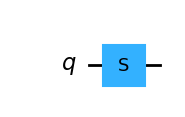
\includegraphics[width=0.3\textwidth]{Images/s-gate.png}
    \caption{S Gate}
    \label{fig:s}
\end{figure}
In the operator Notation it is:
\begin{align*}
    S\ket{0}&=\ket{0} \\
    S\ket{1}&=i\ket{1}
\end{align*}
It is represented by the matrix in the computational basis ($\ket{0},\ket{1}$) as:
\[
    S=\begin{bmatrix}
        1 & 0 \\
        0 & i
    \end{bmatrix}=e^{i\pi/4}\begin{bmatrix}
        e^{-i\pi/4} & 0 \\
        0 & e^{i\pi/4}
    \end{bmatrix}
\]
Thus, it is called as $\pi/4$ gate.
It's Eigen values are 1 and $i$. It's corresponding Eigen vectors are $\ket{0}$ and $\ket{1}$.
It is a Unitary and Hermitian Matrix. It is a Normal Matrix hence Unitarily Diagonalizable.
It has a Spectral decomposition (outer product representation) which can be written as:
\[
    S=\ket{0}\bra{0}+i\ket{1}\bra{1}
\]
Action of S Gate on a general qubit $\ket{\psi}=\alpha\ket{0}+\beta\ket{1}$ is:
\[
    \begin{bmatrix}
        1 & 0 \\
        0 & i
    \end{bmatrix}\begin{bmatrix}
        \alpha \\
        \beta
    \end{bmatrix}=\begin{bmatrix}
        \alpha \\
        i\beta
    \end{bmatrix}=\alpha\ket{0}+i\beta\ket{1}
\]


\subsubsection{$S^{\dagger}$ Gate}
It is $\pi/2$ rotation around Z axis of Bloch Sphere in the opposite direction.
It is also
called as the Conjugate Phase Gate. The truth table is as in table \ref{tab:s-dagger}.
\begin{table}[ht]
    \centering
    \begin{tabular}{|c|c|}
        \hline
        Input & Output\\
        \hline
        $\ket{0}$ & $\ket{0}$\\
        $\ket{1}$ & $-i\ket{1}$\\
        \hline
    \end{tabular}
    \caption{Truth Table for $S^{\dagger}$ Gate}
    \label{tab:s-dagger}
\end{table}
The code for the $S^{\dagger}$ Gate is as follows:
\begin{lstlisting}[language=Python]
from qiskit import QuantumRegister, ClassicalRegister, QuantumCircuit
from numpy import pi

qreg_q = QuantumRegister(1, 'q')
circuit = QuantumCircuit(qreg_q,name='T Gate')

circuit.sdg(qreg_q[0]) #Apply the sdag gate

circuit.draw(output='mpl')#.savefig('../images/sdag-gate.png') #Draw the circuit
\end{lstlisting}

The circuit symbol is as shown in figure \ref{fig:s-dagger}.
\begin{figure}[ht]
    \centering
    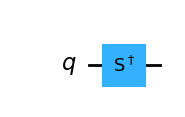
\includegraphics[width=0.3\textwidth]{Images/sdag-gate.png}
    \caption{$S^{\dagger}$ Gate}
    \label{fig:s-dagger}
\end{figure}
In the operator Notation it is:
\begin{align*}
    S^{\dagger}\ket{0}&=\ket{0} \\
    S^{\dagger}\ket{1}&=-i\ket{1}
\end{align*}

It is represented by the matrix in the computational basis ($\ket{0},\ket{1}$) as:
\[
    S^{\dagger}=\begin{bmatrix}
        1 & 0 \\
        0 & -i
    \end{bmatrix}=e^{-i\pi/4}\begin{bmatrix}
        e^{i\pi/4} & 0 \\
        0 & e^{-i\pi/4}
    \end{bmatrix}
\]
It's Eigen values are 1 and $-i$. It's corresponding Eigen vectors are $\ket{0}$ and $\ket{1}$.
It is a Unitary and Hermitian Matrix. It is a Normal Matrix hence Unitarily Diagonalizable.
It has a Spectral decomposition (outer product representation) which can be written as:
\[
    S^{\dagger}=\ket{0}\bra{0}-i\ket{1}\bra{1}
\]
Action of $S^{\dagger}$ Gate on a general qubit $\ket{\psi}=\alpha\ket{0}+\beta\ket{1}$ is:
\[
    \begin{bmatrix}
        1 & 0 \\
        0 & -i
    \end{bmatrix}\begin{bmatrix}
        \alpha \\
        \beta
    \end{bmatrix}=\begin{bmatrix}
        \alpha \\
        -i\beta
    \end{bmatrix}=\alpha\ket{0}-i\beta\ket{1}
\]
\textbf{Note that both $S$ and $S^{\dagger}$ gates are Unitary but not Hermitian thus they are not self-inverse. Recall, that 
the only criteria for a gate is to be a Unitary (from Postulate 2: Unitary evolution) gate and not necessarily Hermitian.}

\subsection{\texorpdfstring{$T$ and $T^{\dagger}$ Gate}{T and T-dagger Gate}}
These are some specialised rotations,
\subsubsection{$T$ Gate}
It is $\pi/4$ rotation around Z axis of Bloch Sphere.
It is also called as the $\pi/8$ Gate. The truth table is as in table \ref{tab:t}.
\begin{table}[ht]
    \centering
    \begin{tabular}{|c|c|}
        \hline
        Input & Output\\
        \hline
        $\ket{0}$ & $\ket{0}$\\
        $\ket{1}$ & $e^{i\pi/4}\ket{1}$\\
        \hline
    \end{tabular}
    \caption{Truth Table for T Gate}
    \label{tab:t}
\end{table}

The code for the T Gate is as follows:
\begin{lstlisting}[language=Python]
from qiskit import QuantumRegister, ClassicalRegister, QuantumCircuit
from numpy import pi

qreg_q = QuantumRegister(1, 'q')
circuit = QuantumCircuit(qreg_q,name='T Gate')

circuit.sdg(qreg_q[0]) #Apply the T gate

circuit.draw(output='mpl')#.savefig('../images/sdag-gate.png') #Draw the circuit    
\end{lstlisting}

The circuit symbol is as shown in figure \ref{fig:t}.
\begin{figure}[ht]
    \centering
    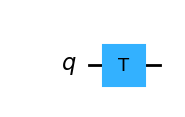
\includegraphics[width=0.3\textwidth]{Images/t-gate.png}
    \caption{T Gate}
    \label{fig:t}
\end{figure}

In the operator Notation it is:
\begin{align*}
    T\ket{0}&=\ket{0} \\
    T\ket{1}&=e^{i\pi/4}\ket{1}
\end{align*}
It is represented by the matrix in the computational basis ($\ket{0},\ket{1}$) as:
\[
    T=\begin{bmatrix}
        1 & 0 \\
        0 & e^{i\pi/4}
    \end{bmatrix}=e^{i\pi/8}\begin{bmatrix}
        e^{-i\pi/8} & 0 \\
        0 & e^{i\pi/8}
    \end{bmatrix}
\]
Thus, it is called as $\pi/8$ gate. This is because up to an unimportant global phase $T$ is equal to a gate which has $e^{\pm \iota \phi/8}$ appearing on its diagonals.
It's Eigen values are 1 and $e^{i\pi/4}$. It's corresponding Eigen vectors are $\ket{0}$ and $\ket{1}$.
It is a Unitary and Hermitian Matrix. It is a Normal Matrix hence Unitarily Diagonalizable.
It has a Spectral decomposition (outer product representation) which can be written as:
\[
    T=\ket{0}\bra{0}+e^{i\pi/4}\ket{1}\bra{1}
\]
Action of T Gate on a general qubit $\ket{\psi}=\alpha\ket{0}+\beta\ket{1}$ is:
\[
    \begin{bmatrix}
        1 & 0 \\
        0 & e^{i\pi/4}
    \end{bmatrix}\begin{bmatrix}
        \alpha \\
        \beta
    \end{bmatrix}=\begin{bmatrix}
        \alpha \\
        e^{i\pi/4}\beta
    \end{bmatrix}=\alpha\ket{0}+e^{i\pi/4}\beta\ket{1}
\]

\subsubsection{$T^{\dagger}$ Gate}
It is $\pi/4$ rotation around Z axis of Bloch Sphere in the opposite direction.
It is also called as the $\pi/8$ Gate. The truth table is as in table \ref{tab:t-dagger}.
\begin{table}[ht]
    \centering
    \begin{tabular}{|c|c|}
        \hline
        Input & Output\\
        \hline
        $\ket{0}$ & $\ket{0}$\\
        $\ket{1}$ & $e^{-i\pi/4}\ket{1}$\\
        \hline
    \end{tabular}
    \caption{Truth Table for $T^{\dagger}$ Gate}
    \label{tab:t-dagger}
\end{table}

The code for the $T^{\dagger}$ Gate is as follows:
\begin{lstlisting}[language=Python]
from qiskit import QuantumRegister, ClassicalRegister, QuantumCircuit
from numpy import pi

qreg_q = QuantumRegister(1, 'q')
circuit = QuantumCircuit(qreg_q,name='T Gate')

circuit.tdg(qreg_q[0]) #Apply the T gate

circuit.draw(output='mpl')#.savefig('../images/tdag-gate.png') #Draw the circuit
\end{lstlisting}

The circuit symbol is as shown in figure \ref{fig:t-dagger}.
\begin{figure}[ht]
    \centering
    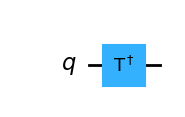
\includegraphics[width=0.3\textwidth]{Images/tdag-gate.png}
    \caption{$T^{\dagger}$ Gate}
    \label{fig:t-dagger}
\end{figure}

In the operator Notation it is:
\begin{align*}
    T^{\dagger}\ket{0}&=\ket{0} \\
    T^{\dagger}\ket{1}&=e^{-i\pi/4}\ket{1}
\end{align*}

One might wonder why the T gate is called the $\pi/8$ gate when it is $\pi/4$ that appears in the definition. The reason is that the gate has historically often been referred to as the $\pi/8$ gate simply because up to an unimportant global phase $T$ is equal to a gate which has $exp(\pm \iota \pi/8)$ appearing on its diagonals. It is represented by the matrix in the computational basis ($\ket{0},\ket{1}$) as:
\[
    T^{\dagger}=\begin{bmatrix}
        1 & 0 \\
        0 & e^{-i\pi/4}
    \end{bmatrix}=e^{-i\pi/8}\begin{bmatrix}
        e^{i\pi/8} & 0 \\
        0 & e^{-i\pi/8}
    \end{bmatrix}
\]
It's Eigen values are 1 and $e^{-i\pi/4}$. It's corresponding Eigen vectors are $\ket{0}$ and $\ket{1}$.
It is a Unitary and Hermitian Matrix. It is a Normal Matrix hence Unitarily Diagonalizable.
It has a Spectral decomposition (outer product representation) which can be written as:
\[
    T^{\dagger}=\ket{0}\bra{0}+e^{-i\pi/4}\ket{1}\bra{1}
\]
Action of $T^{\dagger}$ Gate on a general qubit $\ket{\psi}=\alpha\ket{0}+\beta\ket{1}$ is:
\[
    \begin{bmatrix}
        1 & 0 \\
        0 & e^{-i\pi/4}
    \end{bmatrix}\begin{bmatrix}
        \alpha \\
        \beta
    \end{bmatrix}=\begin{bmatrix}
        \alpha \\
        e^{-i\pi/4}\beta
    \end{bmatrix}=\alpha\ket{0}+e^{-i\pi/4}\beta\ket{1}
\]

Some relations between S and T Gates:
\begin{align*}
    S&=T^2 \\
    S^{\dagger}&=T^{\dagger}T^{\dagger}
\end{align*}
This can be verified as follows. Intuitively, one can think as twice $\pi/4$
rotation around Z axis is $\pi/2$ rotation around Z axis. Thus, the reltaions.
\begin{align*}
    T^2&=\begin{bmatrix}
        1 & 0 \\
        0 & e^{i\pi/4}
    \end{bmatrix}\begin{bmatrix}
        1 & 0 \\
        0 & e^{i\pi/4}
    \end{bmatrix}=\begin{bmatrix}
        1 & 0 \\
        0 & e^{i\pi/2}
    \end{bmatrix}=\begin{bmatrix}
        1 & 0 \\
        0 & i
    \end{bmatrix}=S \\
    T^{\dagger}T^{\dagger}&=\begin{bmatrix}
        1 & 0 \\
        0 & e^{-i\pi/4}
    \end{bmatrix}\begin{bmatrix}
        1 & 0 \\
        0 & e^{-i\pi/4}
    \end{bmatrix}=\begin{bmatrix}
        1 & 0 \\
        0 & e^{-i\pi/2}
    \end{bmatrix}=\begin{bmatrix}
        1 & 0 \\
        0 & -i
    \end{bmatrix}=S^{\dagger}
\end{align*}
\begin{example}
Let $x$ be a real number and $A$ a matrix such that $A^2=I$. Show that
\[
exp(\iota Ax)=\cos (x)I + \iota \sin(x) A
\]

Let $\ket{v}$ be an eignevector of $A$ with eigenvalue $\lambda$. It then follows that $A^2\ket{v}=\lambda^2\ket{v}$, and furthermore we have that $A^2 \ket{v}=I\ket{v}=\ket{v}$ by assumption. We obtain that $\lambda^2= 1$ and therefore the only possible eigenvalues of $A$ are $\lambda=\pm 1$. Let $\ket{v_1},\ldots,\ket{v_k}$ be the eigenvectors with eigenvalue $1$ and $\ket{v_{k+1}},\ldots,\ket{v_n}$ be the eigenvectors with eigenvalue $-1$. By the spectral decompositionm, we can write:
\[
A=\sum_{i=1}^k \ket{v_i}\bra{v_i} - \sum_{i=k+1}^n \ket{v_i}\bra{v_i}
\]
so by the definition of operator functions we have:
\[
exp(\iota Ax)=\sum_{i=1}^k exp(\iota x)\ket{v_i}\bra{v_i} + \sum_{i=k+1}^n exp(-\iota x) \ket{v_i}\bra{v_i}
\]
By Euler's identity we have:
\[
exp(\iota Ax)=\sum_{i=1}^k (\cos(x)+\iota\sin(x))\ket{v_i}\bra{v_i} + \sum_{i=k+1}^n (\cos(x)-\iota \sin(x))\ket{v_i}\bra{v_i}
\]
Grouping terms, we obtain:
\[
exp(\iota Ax)=\cos(x) \sum_{i=1}^n \ket{v_i}\bra{v_i} + \iota \sin(x)\left(\sum_{i=1}^k \ket{v_i}\bra{v_i}-\sum_{i=k+1}^n \ket{v_1}\bra{v_i}\right)
\]
Using the spectral decomposition and definition of $I$, we therefore obtain the desired relation:
\[
exp(\iota Ax)=\cos(x)I+\iota\sin(x)A
\]
\textbf{Since all of the Pauli matrices satisfy $A^2=I$ i.e they are self inverse, for $\theta\in\mathbb{R}$, we can apply this obtained relation. This will be useful for application in Hamiltonian simulation.}
\end{example}
\begin{example}
    \textbf{Functions of the Pauli matrices} let $\vec{v}$ be any real, three-dimensional unit vector and $\theta$ a real number. Let $f(\cdot)$ be any function from complex numbers to complex numbers. Let $\vec{n}$ be a normalized vector in three dimensions, and let $\theta$ be real. Show that
    \[
    f(\theta \vec{n} \cdot \vec{\sigma})=\frac{f(\theta)+f(-\theta)}{2}I+\frac{f(\theta)-f(-\theta)}{2}\vec{n}\cdot \vec{\sigma}
    \]
    where $\vec{n}\cdot\vec{\sigma}=\sum_{i=1}^3 n_i\cdot\sigma_i$, this implies, $\theta\vec{n}\cdot\vec{\sigma}=\sum_{i=1}^3 \theta n_i\cdot\sigma_i$.
    \begin{align*}
    \sum_{i=1}^3 \theta n_i\sigma_i &= \theta n_1 \ket{+}\bra{+}-\theta n_1\ket{-}\bra{-}+\theta n_2\ket{+\iota}\bra{+\iota}-\theta n_2\ket{-\iota}\bra{-\iota} + \theta n_3\ket{0}\bra{0}-\theta n_3\ket{1}\bra{1}\\
    &=\theta \begin{bmatrix} n_3 & n_1-\iota n_2 \\ n_1 + \iota n_2 & -n_3 \end{bmatrix}
    \end{align*}
    where $\vec{n}$ is a real, three dimensional unit vector and $\theta \in \mathbb{R}$, $n_1,n_2,n_3 \in \mathbb{R}$. Note that the above given matrix is clearly a Hermitian matrix, thus has a unitary decomposition (has complete set of eigenvectors spanning $\mathbb{C}^2$). Now, upon solving for the eigen values we get,
    \[
    \begin{vmatrix} n_3 - \lambda & n-1+\iota n_2  \\ n_1+\iota n_2 & -n_2-\lambda \end{vmatrix} = 0
    \]
    this results in the eigenvalues as (using the property of $\vec{n}$ being a unit vector)
    \[
    \lambda=\pm\sqrt{n_1^2+n_2^2+n_3^2}
    \]
    \[
    \lambda=\pm 1
    \]
    Say it's eigen values are $\ket{v_+}$ corresponding to $\lambda=1$ and $\ket{v_-}$ corresponding to $\lambda=-1$. Thus, we get,
    \[
    \vec{n}\cdot\vec{\sigma}=\ket{v_+}\bra{v_+}-\ket{v_-}\bra{v_-}
    \]
    \[
    \sum_{i=1}^3 \theta n_i\sigma_i=\theta (\ket{v_+}\bra{v_+} - \ket{v_-}\bra{v_-})
    \]
    Now,
    \[
    f(\theta \vec{n}\cdot\vec{\sigma})=f(\theta)\ket{v_+}\bra{v_+}+f(-\theta)\ket{v_-}\bra{v_-}
    \]
    From the completeness relationship, we can write Identity as $I=\ket{v_+}\bra{v_+}+\ket{v_-}\bra{v_-}$, hence, For a observable on a 2-dimensional Hilbert space with eigenvalues$\lambda=\pm 1$ has projectors
    \begin{align*}
    \frac{I+\vec{n}\cdot\vec{\sigma}}{2}&=\ket{v_+}\bra{v_+}\\
    \frac{I-\vec{n}\cdot\vec{\sigma}}{2}&=\ket{v_-}\bra{v_-}
    \end{align*}
    Substituting this in the equation we get,
    \[
    f(\theta\vec{n}\cdot\vec{\sigma})=f(\theta)\frac{I+\vec{n}\cdot\vec{\sigma}}{2}+f(-\theta)\frac{I-\vec{n}\cdot\vec{\sigma}}{2}
    \]
    On simplifying this we get,
    \[
    f(\theta\vec{n}\cdot\vec{\sigma})=\frac{f(\theta)+f(-\theta)}{2}I+\frac{f(\theta)-f(-\theta)}{2}\vec{n}\cdot\vec{\sigma}
    \]
    In case we write the function as $exp(\iota \theta\vec{n}\cdot\vec{\sigma})$ we get,
    \[
    exp(\iota\theta\vec{n}\cdot\vec{\sigma})=\cos(\theta)I+\iota\sin(\theta) \vec{n}\cdot\vec{\sigma}
    \]
    \end{example}


\subsection{Quantum Rotation Gates}
These are generalized rotations  in the Bloch Sphere 
denoted as $R_X,R_Y,R_Z$ about the X,Y and Z axis of Bloch Sphere respectively. The Pauli matrices give rise to three useful classes of Unitary matrices when they are exponentiated, the rotation operators about the $x,y,z$ axes.
\subsubsection{$R_X$ Gate}
It is a rotation about X axis of Bloch Sphere by an angle $\theta$. Putting $\vec{n}=(1,0,0)$ in the previous equation and putting $\theta=-\theta/2$. This is denoted
as $R^{X}_{\theta}$.
The matrix representation of $R^{X}_{\theta}$ is:
\[
    R^{X}_{\theta}=\begin{bmatrix}
        \cos(\theta/2) & -i\sin(\theta/2) \\
        -i\sin(\theta/2) & \cos(\theta/2)
    \end{bmatrix}=\cos \frac{\theta}{2}I-\iota \sin\frac{\theta}{2}\sigma_X=e^{-\iota\frac{\theta}{2}\sigma_X}
\]
The code for the $R_X$ Gate is as follows:
\begin{lstlisting}[language=Python]
from qiskit import QuantumRegister, ClassicalRegister, QuantumCircuit
from numpy import pi

qreg_q = QuantumRegister(1, 'q')
circuit = QuantumCircuit(qreg_q,name='U1 Gate')

circuit.rx(pi/2,qreg_q[0]) #Apply the RX gate

circuit.draw(output='mpl')#.savefig('../images/rx-gate.png') #Draw the circuit
\end{lstlisting}

The circuit symbol is as shown in figure \ref{fig:rx}.
\begin{figure}[ht]
    \centering
    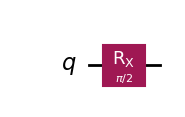
\includegraphics[width=0.3\textwidth]{Images/rx-gate.png}
    \caption{$R_X$ Gate}
    \label{fig:rx}
\end{figure}
Note that the value $\pi/2$ given in the figure \ref{fig:rx} denotes the angle by which we rotate around the X Axis of Bloch Sphere. Note that $R_{\pi}^{X} = -\iota X$.

\subsubsection{$R_Y$ Gate}
It is a rotation about Y axis of Bloch Sphere by an angle $\theta$. This is denoted
as $R^{Y}_{\theta}$.
The matrix representation of $R^{Y}_{\theta}$ is:
\[
    R^{Y}_{\theta}=\begin{bmatrix}
        \cos(\theta/2) & -\sin(\theta/2) \\
        \sin(\theta/2) & \cos(\theta/2)
    \end{bmatrix}= \cos \frac{\theta}{2}I-\iota \sin \frac{\theta}{2}\sigma_Y=e^{-\iota \frac{\theta}{2}\sigma_Y}
\]
The code for the $R_Y$ Gate is as follows:
\begin{lstlisting}[language=Python]
from qiskit import QuantumRegister, ClassicalRegister, QuantumCircuit
from numpy import pi

qreg_q = QuantumRegister(1, 'q')
circuit = QuantumCircuit(qreg_q,name='RY Gate')

circuit.ry(pi/2,qreg_q[0]) #Apply the RY gate

circuit.draw(output='mpl')#.savefig('../images/ry-gate.png') #Draw the circuit
\end{lstlisting}

The circuit symbol is as shown in figure \ref{fig:ry}.
\begin{figure}[ht]
    \centering
    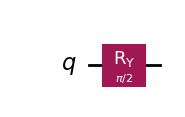
\includegraphics[width=0.3\textwidth]{Images/ry-gate.png}
    \caption{$R_Y$ Gate}
    \label{fig:ry}
\end{figure}
Note here the value $\pi/2$ denotes the angle by which we rotate around the Y Axis of Bloch Sphere. Note that $R_{\pi}^Y=-\iota Y$.

\subsubsection{$R_Z$ Gate}
It is a rotation about Z axis of Bloch Sphere by an angle $\theta$. This is denoted
as $R^{Z}_{\theta}$.
The matrix representation of $R^{Z}_{\theta}$ is:
\[
    R^{Z}_{\theta}=\begin{bmatrix}
        e^{-i\theta/2} & 0 \\
        0 & e^{i\theta/2}
    \end{bmatrix}=\cos \frac{\theta}{2}I-\iota \sin \frac{\theta}{2}\sigma_Z=e^{-\iota \frac{\theta}{2}\sigma_Z}
\]

The code for the $R_Z$ Gate is as follows:
\begin{lstlisting}[language=Python]
from qiskit import QuantumRegister, ClassicalRegister, QuantumCircuit
from numpy import pi

qreg_q = QuantumRegister(1, 'q')
circuit = QuantumCircuit(qreg_q,name='RZ Gate')

circuit.rz(pi/2,qreg_q[0]) #Apply the RZ gate

circuit.draw(output='mpl')#.savefig('../images/rz-gate.png') #Draw the circuit
\end{lstlisting}

The circuit symbol is as shown in figure \ref{fig:rz}.
\begin{figure}[ht]
    \centering
    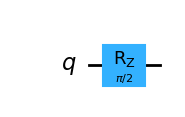
\includegraphics[width=0.3\textwidth]{Images/rz-gate.png}
    \caption{$R_Z$ Gate}
    \label{fig:rz}
\end{figure}
Note here the value $\pi/2$ denotes the angle by which we rotate around the Z Axis of Bloch Sphere. Note that $R_{\pi}^Z = -\iota Z$.

This Quantum Rotation Gates can be used in making variational circuit as angles can vary.

\subsubsection{$R_n$ \textbf{Gate}}
If $\hat{n}=(n_x,n_y,n_z)$ is a real unit vector in three dimensions then we generalize the previous definitions by defining a rotation by $\theta$ about the $\hat{n}$ axis by the equation
\[
R_{\hat{n}}(\theta)=exp(-\iota \theta \hat{n}\cdot \vec{\sigma}/2)=\cos \left(\frac{\theta}{2}\right)I- \iota \sin \left(\frac{\theta}{2}\right) (n_xX+n_yY+n_zZ)
\]
where $\vec{\sigma}$ denotes the three component vector $(X,Y,Z)$ of Pauli matrices. Thus, in matrix form, we can write $R_n(\theta)$ as:
\[
\begin{bmatrix} \cos \frac{\theta}{2} - \iota \sin \frac{\theta}{2} n_z & -\sin \frac{\theta}{2} (n_y+\iota n_x)\\ \sin \frac{\theta}{2} (n_y-\iota n_x) & \cos\frac{\theta}{2} + \iota \sin \frac{\theta}{2} n_z \end{bmatrix}
\]
\subsection{Universal Quantum Gates}
To construct any single qubit Quantum gates.
\[
    U_3(\theta,\phi,\lambda)=\begin{bmatrix}
        \cos(\theta/2) & -e^{i\lambda}\sin(\theta/2) \\
        e^{i\phi}\sin(\theta/2) & e^{i(\phi+\lambda)}\cos(\theta/2)
    \end{bmatrix}
\]
where $\theta,\phi,\lambda\in\mathbb{R}$ are rotations around x, y and z axis respectively.
Here, $0 \leq \theta \leq \pi$, $0\leq \phi \leq 2\pi$ and $0\leq \lambda \leq 2\pi$.
Similarly, we can fix $\theta$ and write $U_2$ gate as:
\[
    U_2(\phi,\lambda)=\begin{bmatrix}
        1 & -e^{i\lambda} \\
        e^{i\phi} & e^{i(\phi+\lambda)}
    \end{bmatrix}
\]
Here $\theta=\pi/2$ by default.
Similarly, we can fix $\theta$ and $\phi$ and write $U_1$ gate as:
\[
    U_1(\lambda)=\begin{bmatrix}
        1 & 0 \\
        0 & e^{i\lambda}
    \end{bmatrix}
\]
Here $\theta=\phi=0$ by default.

The code for the $U_3$ Gate is as follows:
\begin{lstlisting}[language=Python]
from qiskit import QuantumRegister, ClassicalRegister, QuantumCircuit
from numpy import pi

qreg_q = QuantumRegister(1, 'q')
circuit = QuantumCircuit(qreg_q,name='U3 Gate')

circuit.u(pi/2,pi/2,pi/2,qreg_q[0]) #Apply the U3 gate

circuit.draw(output='mpl')#.savefig('../images/u3-gate.png') #Draw the circuit
\end{lstlisting}

The circuit symbol is as shown in figure \ref{fig:u3}.
\begin{figure}[ht]
    \centering
    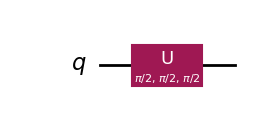
\includegraphics[width=0.3\textwidth]{Images/u3-gate.png}
    \caption{$U_3$ Gate}
    \label{fig:u3}
\end{figure}
Note here the values $\pi/2,\pi/2,\pi/2$ denotes the angles $\theta,\phi,\lambda$ by which we rotate around the Bloch Sphere respectively.

\begin{example}
    Show that, up to a global phase, the $\pi/8$ gate satisfies $T=R_z(\pi/4)$

    Recall that the $T$ gate is defined as:
    \[
    T=\begin{bmatrix} 1 & 0 \\ 0 & exp(\iota \pi/4) \end{bmatrix}
    \]
    We observe that:
    \[
    R_z(\pi/4)=\begin{bmatrix} e^{-\iota \pi/8} & 0 \\ 0 & e^{\iota \pi/8} \end{bmatrix}=e^{-\iota \pi/8}\begin{bmatrix} 1 & 0 \\ 0 & e^{\iota \pi/4} \end{bmatrix} = e^{-\iota \pi/8}T
    \]
\end{example}

\begin{example}
    Express the Hadamard gate $H$ as a product of $R_x$ and $R_z$ rotations and $e^{\iota \varphi}$ for some $\varphi$.

    We claim that $H=R_z(\pi/2)R_x(\pi/2)R_z(\pi/2)$ up to a global phase of $e^{-\iota \pi/2}$. Doing a computation to verify this claim, we see that:
    \begin{align*}
    R_z(\pi/2)R_x(\pi/2)R_z(\pi/2)&=\begin{bmatrix} e^{-\iota \pi/4} & 0 \\ 0 & e^{\iota \pi/4} \end{bmatrix} \begin{bmatrix} \cos(\frac{\pi}{4}) & -\iota \sin(\frac{\pi}{4}) \\ - \iota \sin (\frac{\pi}{4}) & \cos(\frac{\pi}{4}) \end{bmatrix}\begin{bmatrix} e^{-\iota \pi/4} & 0 \\ 0 &e^{\iota \pi/4} \end{bmatrix}\\
    &=\begin{bmatrix} e^{-\iota \pi/4} & 0 \\ 0 & e^{\iota \pi/4} \end{bmatrix} \begin{bmatrix}\frac{1}{\sqrt{2}} & -\frac{\iota}{\sqrt{2}} \\ -\frac{\iota}{\sqrt{2}} & \frac{1}{\sqrt{2}} \end{bmatrix}\begin{bmatrix} e^{-\iota \pi/4} & 0 \\ 0 &e^{\iota \pi/4} \end{bmatrix}\\
    &=\frac{1}{\sqrt{2}} \begin{bmatrix} e^{-\iota \pi/4} & 0 \\ 0 & e^{\iota \pi/4} \end{bmatrix}\begin{bmatrix} e^{-\iota \pi/4} & -\iota e^{\iota\pi/4} \\ -\iota e^{-\iota \pi/4} & e^{\iota \pi/4} \end{bmatrix}\\
    &=\frac{1}{\sqrt{2}}\begin{bmatrix} e^{-\iota \pi/2} & -e^{\iota \pi/2} \\ - e^{-\iota \pi/2} & e^{\iota \pi/2} \end{bmatrix}\\
    &=\frac{e^{-\iota \pi/2}}{\sqrt{2}}\begin{bmatrix} 1 & 1 \\ 1 & -1 \end{bmatrix}\\
    &=e^{-\iota \pi/2} H
    \end{align*}
    Thus, we get,
    \[
    e^{\iota \pi/2} R_z(\pi/2)R_x(\pi/2)R_z(\pi/2) =H
    \]
\end{example}

\begin{example}
    Prove that $(\hat{\mathbf{n}}\cdot \mathbf{\sigma})^2 = I$

    \begin{align*}
    (\hat{\mathbf{n}}\cdot \mathbf{{\sigma}})^2 &= (n_xX+n_yY+n_zZ)^2\\
    &=n_x^2X^2+n_y^2 Y+n_z^2 Z^2 +n_xn_y(XY+YX)+n_xn_z(XZ+ZX)+n_yn_z(YZ+ZY)
    \end{align*}
Recall that $\{\sigma_i,\sigma_j\}=2\delta_{ij}I$, using this, we have that:
\[
(\hat{\mathbf{n}} \cdot \mathbf{\sigma})^2 =(n_z^2 + n_y^2 + n_z^2)I=I
\]
where we use the fact that $\hat{\mathbf{n}}$ is a vector of unit length.
\end{example}

\begin{example}
    One reason why the $\hat{R}_n(\theta)$ operators are referred to as rotation operators is the following fact, which you are to prove. Suppose a single qubit has a state represented by the Bloch vector $\mathbf{\lambda}$. Then, the effects of the rotation $\hat{R}_n(\theta)$ on the state is to rotate by an angle $\theta$ about the $\hat{n}$ axis of the Bloch sphere. This fact explains the rather mysterious looking factors of two in the definition of the rotation matrices.

    Let $\mathbf{\lambda}$ be an arbitrary Bloch vector. Without the loss of generality, we can express $\mathbf{\lambda}$ in a coordinate system such that $\hat{n}$ is aligned with $z$ axis, so it suffices to consider how the state behaves under the application $R_z(\theta)$. Let $\mathbf{\lambda}=()$ be the vector expressed in this coordinate system. We know that the density operator corresponding to this Bloch vector is given by:
    \[
    \rho=\frac{I+\mathbf{\lambda} \cdot \mathbf{\sigma}}{2}
    \]
    We now observe how $\rho$ transforms under the conjugation of $R_z(\theta)$.
    \begin{align*}
        R_z(\theta)\rho R_z(\theta)^{\dagger} &=R_z(\theta)\rho R_z(-\theta)\\
        &=R_z(\theta)\left(\frac{I+\lambda_xX+\lambda_yY+\lambda_zZ}{2}\right)R_z(-\theta)
    \end{align*}
    Using that $XZ=-ZX$, we make the observation that:
    \begin{align*}
        R_z(\theta)X&=\left(\cos \left(\frac{\theta}{2}\right)I-\iota \sin\left(\frac{\theta}{2}\right)Z \right) X\\
        &=X\left(\cos \left(\frac{\theta}{2}\right)I+\iota \sin\left((\frac{\theta}{2}\right)Z\right)\\
        &=X\left(\cos\left(\frac{-\theta}{2}\right)I-\iota \sin\left(\frac{-\theta}{2}\right)Z\right)\\
        &=XR_z(-\theta)
    \end{align*}
    Similarly, we find that $R_z(\theta)Y=YR_z(-\theta)$ (same anticommutation) and that $R_z(\theta)Z=ZR_z(\theta)$ (all terms commute). With this, for expression $R_z(\theta)\rho R_z(\theta)^{\dagger}$ simplifies to:
    \begin{align*}
        R_z(\theta)\rho R_z(\theta)^{\dagger}&=R_z(\theta)\left(\frac{I+\lambda_zX+\lambda_yY+\lambda_zZ}{2}\right) R_z(-\theta)\\
        &= \frac{I+\lambda_xXR_z(-2\theta)+\lambda_yYR_z(-2\theta)+\lambda_zZ}{2}
    \end{align*}
    Calculating each of the terms in the above expression, we have:
    \begin{align*}
        XR_z(-2\theta)&=X\left(\cos\left(\frac{-2\theta}{2}\right)-\iota \sin\left(\frac{-2\theta}{2}\right) Z\right)\\
        &=X(\cos(\theta)+\iota \sin(\theta)Z)\\
        &=\cos(\theta)X+\iota \sin(\theta)XZ\\
        &=\cos(\theta)X+\iota \sin(\theta)(-\iota Y)\\
        &=\cos(\theta)X+\sin(\theta)Y\\
        YR_z(-2\theta)&=Y(\cos(\theta)+\iota \sin(\theta)Z)\\
        &=\cos(\theta)Y+\iota \sin(\theta)YZ\\
        &=\cos(\theta)Y+\iota \sin(theta)(\iota X)\\
        &=\cos(\theta)Y-\sin(\theta)X
    \end{align*}
    Plugging these back into the expression for $R_z(\theta)\rho R_z(\theta)^{\dagger}$ and collecting like terms, we have:
    \[
    R_z(\theta)\rho R_z(\theta)^{\dagger}=\frac{I+(\lambda_x\cos(\theta)-\lambda_y\sin(\theta))X+(\lambda_x\sin(\theta)+\lambda_y\cos(\theta))Y+\lambda_zZ}{2}
    \]
    From this expression, we can read off the new Bloch vector $\mathbf{\lambda'}$ after conjugation by $R_z(\theta)$ to be:
    \[
    \mathbf{\lambda'}=(\lambda_x\cos(\theta)-\lambda_y \sin(\theta),\lambda_x\sin(\theta)+\lambda_y\cos(\theta),\lambda_z)
    \]
    Alternatively, suppose we apply the 3-dimensional rotation matrix $A_z(\theta)$ to the original bloch vector $\mathbf{\lambda}$. We have that:
    \[
    A_z(\theta)\mathbf{\lambda}=\begin{bmatrix}\cos\theta & -\sin\theta & 0 \\ \sin\theta & \cos\theta & 0 \\ 0 & 0 & 1 \end{bmatrix} \begin{bmatrix} \lambda_x \\ \lambda_y \\ \lambda_z \end{bmatrix}=\begin{bmatrix} \lambda_x \cos\theta-\lambda_y \sin\theta \\ \lambda_x\sin\theta+\lambda_y \cos\theta \\ \lambda_z \end{bmatrix}
    \]
    We see that we end up with the same resulting vector $\mathbf{\lambda'}$. We conclude that the conjugation of $\rho$ under $R_z(\theta)$ has the equivalent effect to rotating the Bloch vector by $\theta$ about the z-axis, and hence the effect of $R_n(\theta)$ on one qubit state is to rotate it by an angle $\theta$ about $\hat{\mathbf{n}}$.
    % Alternatively, we can also think of this in a different way as we can write any $\ket{\lambda}= \begin{bmatrix} \cos{\frac{\theta}{2}} \\ e^{\iota \phi}\sin{\frac{\theta}{2}} \end{bmatrix}$ in the $\ket{0},\ket{1}$ basis. Thus, the action of $R_z(\theta)$ on this vector will be
    % \begin{align*}
    % R_z(\theta)\ket{\lambda} &= \cos{\frac{\theta}{2}} \begin{bmatrix} \cos{\frac{\theta}{2}} \\ e^{\iota \phi}\sin{\frac{\theta}{2}} \end{bmatrix} - \iota \sin{\frac{\theta}{2}} \begin{bmatrix} 1 & 0 \\ 0 & -1 \end{bmatrix}\begin{bmatrix} \cos{\frac{\theta}{2}} \\ e^{\iota \phi}\sin{\frac{\theta}{2}} \end{bmatrix}\\
    % &=\begin{bmatrix} e^{-\iota\frac{\theta}{2}} & 0 \\ 0 & e^{\iota \frac{\theta}{2}} \end{bmatrix} \begin{bmatrix} \cos{\frac{\theta}{2}} \\ e^{\iota \phi}\sin{\frac{\theta}{2}} \end{bmatrix}\\
    % &=\begin{bmatrix} e^{-\iota \frac{\theta}{2}}\cos{\frac{\theta}{2}} \\ e^{\iota \phi +\iota \frac{\theta}{2}}\sin{\frac{\theta}{2}} \end{bmatrix}
    % \end{align*}
    % Thus, the state can then be written as $e^{-\iota \frac{\theta}{2}} (\cos(\frac{\theta}{2})\ket{0} + e^{\iota (\phi + \theta)}\sin(\frac{\theta}{2}) \ket{1})$. Ignoring the global phase, we can write this as, $\cos(\frac{\theta}{2})\ket{0} + e^{\iota (\phi + \theta)}\sin(\frac{\theta}{2}) \ket{1}$. Thus, we see that the 

    % Recall that, $R_n(\theta)=\cos(\frac{\theta}{2})I-\iota \sin(\frac{\theta}{2}) (n_x X+n_yY+n_zZ)$, thus we can write $\vec{\lambda} = (\sin{\theta} \cos\phi , \sin \theta \sin \phi, \cos \theta)$.
\end{example}

\begin{example}
    Show that $XYX=-Y$ and use this to prove that $XR_y(\theta)X=R_y(-\theta)$.

    For the first, claim we use that $XY=-YX$ and $X^2=I$ to obtain that
    \[
    XYX=-YXX=-YI=-Y
    \]
    Using this, we have that:
    \begin{align*}
    XR_y(\theta)X&=X\left(\cos\left(\frac{\theta}{2}\right)I-\iota\sin\left(\frac{\theta}{2}\right)Y\right)X\\
    &=\cos\left(\frac{\theta}{2}\right)XIX-\iota \sin\left(\frac{\theta}{2}\right)XYX\\
    &=\cos\left(\frac{\theta}{2}\right) I+\iota \sin\left(\frac{\theta}{2}\right)Y\\
    &=\cos\left(-\frac{\theta}{2}\right)I-\iota \sin\left(-\frac{\theta}{2}\right)Y\\
    &=R_y(-\theta)
    \end{align*}
\end{example}

\begin{example}
    An arbitrary single qubit unitary operator can be written in the form
    \[
    U=exp(\iota \alpha)R_n(\theta)
    \]
    for some real numbers $\alpha$ and $\theta$, and a real three-dimensional unit vector $\hat{n}$.
    \begin{enumerate}
        \item Prove this fact.
        \item Find values for $\alpha$,$\theta$, and $\hat{n}$ giving the Hadamard gate $H$.
        \item Find values for $\alpha,\theta$ and $\hat{n}$ giving the phase gate
        \[
        S=\begin{bmatrix} 1 & 0 \\ 0 & \iota \end{bmatrix}
        \]
    \end{enumerate}
    \begin{enumerate}
        \item By definition, for any unitary operator $U$ we have that $U^{\dagger}U=I$, so for any state vector $\braket{\psi|\psi}=\bra{\psi}U^{\dagger}U\ket{\psi}$. Therefore, all unitary Us are norm-preserving, and hence for a single qubit correspond to some reflection/rotation in 3-dimensional space (up to a global phase factor). Hence, we can write $U=exp(\iota \alpha)R_n(\theta)$ for some $\hat{n}$ (rotation axis), $\theta$ (rotation angle) and $\alpha$(global phase). Any $2\times 2$ unitary matrix for $a^2+b^2+c^2+d^2=1$ can be written as,
        \[
        U=e^{\iota \alpha} \begin{bmatrix} a +\iota b & c+\iota d \\ -c+\iota d & a-\iota b \end{bmatrix}
        \]
        Consider, the given form for $U$. Note that we can write $R_n(\theta)=e^{-\iota \frac{\theta}{2} (n\cdot \sigma)}$ by substituting the values of $X, Y, Z$ pauli matrices and thus arriving at the following matrix as:
        \[
        U=e^{\iota \alpha}\begin{bmatrix} \cos \frac{\theta}{2} - \iota \sin \frac{\theta}{2} n_z & -\sin \frac{\theta}{2} (n_y+\iota n_x)\\ \sin \frac{\theta}{2} (n_y-\iota n_x) & \cos\frac{\theta}{2} + \iota \sin \frac{\theta}{2} n_z \end{bmatrix}
        \]
        As, $n_x^2+n_y^2+n_z^2=1$ this has the same form as the general $U$, also, there are four independent variables- any two of the $n_x,n_y,n_z$ as they are constrained by the equation $n_x^2+n_y^2+n_z^2=1$ and $\theta, \alpha$. hence any arbitrary $2\times 2$ unitary matrix can be written as $U=e^{\iota \alpha}R_n(\theta)$.
        \item Using the fact that $H=\frac{X+Z}{\sqrt{2}}$, and that modulo factor of $\iota$ that $X/Z$ correspond to rotations $R_x(\pi)$ and $R_z(\pi)$, we find that:
        \begin{align*}
            H=\frac{\iota R_x(\pi)+\iota R_z(\pi)}{\sqrt{2}}&=\iota\left(\frac{2\cos{\frac{\pi}{2}}I-\iota \sin\frac{\pi}{2}X-\iota 
            \sin\frac{\pi}{2} Z}{\sqrt{2}}\right)\\
            &=e^{\iota \frac{\pi}{2}} \left(\cos\left(\frac{\pi}{2}\right)I-\iota \sin\left(\frac{\pi}{2}\right)\left(\frac{1}{\sqrt{2}}X+0Y+\frac{1}{\sqrt{2}}Z\right)\right)
        \end{align*}
        Note that in the second equality we use that $\cos\left(\frac{\pi}{2}\right)=0$ and hence $\frac{2}{\sqrt{2}}\cos\left(\frac{\pi}{2}\right)=\cos\left(\frac{\pi}{2}\right)$. From the last expression, we can read off using the definition of $R_n(\theta)$ that $n=\left(\frac{1}{\sqrt{2}},0,\frac{1}{\sqrt{2}}\right)$,$\theta=\pi$, and $\alpha=\frac{\pi}{2}$.
        \item We observe that:
        \[
        R_z\left(\frac{\pi}{2}\right)=\begin{bmatrix} e^{-\iota \pi/4} & 0 \\ 0 & e^{\iota \pi/4} \end{bmatrix}=e^{-\iota \pi/4}\begin{bmatrix} 1 & 0 \\ 0 & \iota \end{bmatrix}
        \]
        Hence:
        \[
        S=e^{\iota \pi/4}R_z\left(\frac{\pi}{2}\right)
        \]
        from which we obtain that $\hat{n}=\hat{z}=(0,0,1),\theta=\frac{\pi}{2}$, and $\alpha=\frac{\pi}{4}$.
    \end{enumerate}
    Note that one can just use the definition:
    \[
    R_n(\theta)=exp(-\iota \theta \hat{n}\cdot \sigma/2)=\cos\left(\frac{\theta}{2}\right)I-\iota \sin\left(\frac{\theta}{2}\right)(n_xX+n_yY+n_zZ)
    \]
    and the fact that $H=(X+Z)/\sqrt{2}$, to arrive at $\cos\left(\frac{\theta}{2}\right)=0,n_x=n_z=\frac{1}{\sqrt{2}},n_y=0$.
\end{example}

An arbitrary unitary operator on a single qubit can be written in many ways as a combination of rotations, together with global phase shifts on the qubit. The following theorem provides a means of expressing an arbitrary single qubit rotation that will be particularly useful in later applications to controlled operations.

\begin{theorem}
    \textbf{(Z-Y decomposition for a single qubit)} Suppose $U$ is a unitary operation on a single qubit. Then there exist a real number $\alpha,\beta,\gamma$ and $\delta$ such that
    \[
    U=e^{\iota \alpha} R_z(\beta)R_y(\gamma)R_z(\delta)
    \]
\end{theorem}
\begin{proof}
    Since $U$ is unitary, the rows and columns of $U$ are orthonormal, from which it follows that there exist real numbers $\alpha,\beta,\gamma,$ and $\delta$ such that
    \[
    U=\begin{bmatrix} e^{\iota (\alpha - \beta/2 -\delta/2)} \cos \frac{\gamma}{2} & -e^{\iota (\alpha-\beta/2+\delta/2}\sin\frac{\gamma}{2}\\
    e^{\iota (\alpha+\beta/2-\delta/2)}\sin\frac{\gamma}{2} & e^{\iota(\alpha+\beta/2+\delta/2}\cos \frac{\gamma}{2} \end{bmatrix}
    \]
    Thus, the equation now follows immediately from the definition of the rotation matrices and matrix multiplication.
\end{proof}
\begin{example}
    Explain why any single qubit unitary operator may be written in the previous form.

    Let $U$ be a single qubit unitary operator. we then have that $U^{\dagger}U=I$, so identifying: 
    \[
    U=\begin{bmatrix} a & b \\ c & d \end{bmatrix} = \begin{bmatrix} \mathbf{v_1} & \mathbf{v_2} \end{bmatrix}
    \]
    we obtain that:
    \[
    \begin{bmatrix} |a|^2 + |c|^2 & a^*b+c^*d \\ ab^*+cd^* & |b|^2+|d|^2 \end{bmatrix} = \begin{bmatrix} 1 & 0 \\ 0 & 1 \end{bmatrix}
    \]
    From the diagonal entries we obtain that $|a|^2+|c|^2=1$ and $|b|^2+|d|^2=1$ and from the off-diagonal entries we obtain that $\braket{v_1,v_2}=0$, and hence the columns of $U$ are orthonormal. From the fact that $|v_1|$ is normalized, we can parametrize the magnitude of the entries with $\gamma \in \mathbb{R}$ such that:
    \[
    |a|=\cos \frac{\gamma}{2}, \quad |c|=\sin \frac{\gamma}{2}
    \]
    from the orthogonality $U^{\dagger}=U^{-1}$ we get, 
    \[
    U^{-1}=\begin{bmatrix} d & -b \\ -c & a \end{bmatrix} =U^{\dagger} = \begin{bmatrix} a^* & c^* \\ b^* & d^* \end{bmatrix}
    \]
    we further obtain that $b=-c^*$ and $d=a^*$, from which we have that $|b|=|c|$ and $|d|=|a|$. Thus, we have the following matrix:
    \[
    U=\begin{bmatrix} a & -c^* \\c & a^* \end{bmatrix}
    \]
    Furthermore, (also from orthogonality) we can parametrize such that for any $arg(a)=-\frac{\beta}{2}-\frac{\delta}{2}$ and $arg(b)=\frac{\beta}{2} - \frac{\delta}{2}$. For $\beta,\delta \in \mathbb{R}$. Finally, multiplying $U$ by a complex phase $e^{\iota \alpha}$ for $\alpha \in \mathbb{R}$ preserves the unitarity of $U$ and the orthonormality of the columns. Combining these facts gives the form as desired.
    We can write,
    \[
    U=\begin{bmatrix} e^{\iota (\alpha - \beta/2 -\delta/2)} \cos \frac{\gamma}{2} & -e^{\iota (\alpha-\beta/2+\delta/2)}\sin\frac{\gamma}{2}\\
    e^{\iota (\alpha+\beta/2-\delta/2)}\sin\frac{\gamma}{2} & e^{\iota(\alpha+\beta/2+\delta/2)}\cos \frac{\gamma}{2} \end{bmatrix}=e^{\iota \alpha} \begin{bmatrix} e^{\iota (- \beta/2 -\delta/2)} \cos \frac{\gamma}{2} & -e^{\iota (-\beta/2+\delta/2)}\sin\frac{\gamma}{2}\\
    e^{\iota (\beta/2-\delta/2)}\sin\frac{\gamma}{2} & e^{\iota(\beta/2+\delta/2)}\cos \frac{\gamma}{2} \end{bmatrix}
    \]
    \[
    =e^{\iota \alpha}\begin{bmatrix} a & -c^* \\ c & a^* \end{bmatrix}
    \]
    which is the general form of a $2\times 2$ unitary matrix as $det(U)=\cos^2 \frac{\gamma}{2} + \sin^2 \frac{\gamma}{2}=1$.
\end{example}
\begin{example}
    \textbf{(X-Y decomposition of rotations)} Give a decomposition analogous to the previous theorem but using $R_x$ instead of $R_z$.

    
We simply use the fact that we can do a change of reference, to interchange the $x$ and $z$ axes. We know that the hadamard $H$ is unitary and self-inverse implements the appropriate swap between $x$ and $z$ axes, while send $y$ to $-y$. So instead of working with $U$ directly, consider
\[
U'=HUH^{-1 }= HUH
\]
which is the frame-rotated $U$. Now, we can use the following ZY decomposition of $U'$.
\[
U'=e^{\iota \alpha}R_z(\beta)R_y(\gamma)R_z(\delta)
\]
What does this imply for $U$? We will see that the above implies an XY-decomposition for $U$.
\begin{align*}
    U=HU'H&=e^{\iota \alpha}(HR_z(\beta)H)(HR_y(\gamma)H)(HR_z(\delta)H)\\
    &=e^{\iota \alpha} R_x(\beta)R_y(-\gamma)R_x(\delta)
\end{align*}
\end{example}
\begin{example}
    Suppose $\hat{m}$ and $\hat{n}$ are non-parallel real unit vectors in three dimensions. Use the theorem to show that an arbitrary single qubit unitary $U$ may be written
    \[
    U=e^{\iota \alpha} R_{\hat{n}}(\beta)R_{\hat{m}}(\gamma)R_{\hat{n}}(\delta)
    \]
    for appropriate choices of $\alpha,\beta,\gamma$ and $\delta$.
    The same arguments in above example could be generalize. We could choose any two orthogonal axes $\hat{n},\hat{m}$ for rotations in our decomposition, using the fact that we can always frame rotate to $z$ and $x$ axes.
\end{example}

Consider the following corollary, which is the key to the construction of controlled multi-qubit unitary operations, as explained.

\begin{corollary}
    Suppose $U$ is a unitary gate on a single qubit. Then there exist unitary operators $A,B,C$ on a single qubit such that $ABC=I$ and $U=e^{\iota \alpha}AXBXC$, where $\alpha$ is some overall phase factor.
\end{corollary}
\begin{proof}
    Set $A=R_z(\beta)R_y(\gamma/2), B=R_y(-\gamma/2)R_z(-(\delta+\beta)/2)$ and $C=R_z((\delta-\beta)/2)$. Note that
    \[
    ABC=R_z(\beta)R_y\left(\frac{\gamma}{2}\right)R_y\left(-\frac{\gamma}{2}\right)R_z\left(-\frac{\delta+\beta}{2}\right)R_z\left(\frac{\delta-\beta}{2}\right)
    \]
    Since $X^2=I$ and $XR_Y(\theta)X=R_y(-\theta)$, we see that,
    \[
    XBX=XR_y\left(-\frac{\gamma}{2}\right)XXR_z\left(-\frac{\delta+\beta}{2}\right)X=R_y\left(\frac{\gamma}{2}\right)R_z\left(\frac{\delta+\beta}{2}\right)
    \]
    Thus
    \begin{align*}
    AXBXC&=R_z(\beta)R_y\left(\frac{\gamma}{2}\right)R_y\left(\frac{\gamma}{2}\right)R_z\left(\frac{\delta+\beta}{2}\right)R_z\left(\frac{\delta-\beta}{2}\right)\\
    &=R_z(\beta)R_y(\gamma)R_z(\delta)
    \end{align*}
    Thus, $U=e^{\iota\alpha}AXBXC$ and $ABC=I$, as required.
\end{proof}

\begin{example}
    Give $A,B,C$ and $\alpha$ for the Hadamard Gate.

    From the proof recall that $U$ is unitary such that
    \[
    U=\begin{bmatrix} e^{\iota (\alpha - \beta/2 -\delta/2)} \cos \frac{\gamma}{2} & -e^{\iota (\alpha-\beta/2+\delta/2)}\sin\frac{\gamma}{2}\\
    e^{\iota (\alpha+\beta/2-\delta/2)}\sin\frac{\gamma}{2} & e^{\iota(\alpha+\beta/2+\delta/2)}\cos \frac{\gamma}{2} \end{bmatrix}
    \]
    This matrix becomes $H$ when $\alpha=\gamma=\frac{\pi}{2},\delta=\pi,\beta=0$. Thus, from the previous corollary, we see that $A=R_z(\beta)R_y(\gamma/2)=R_y\left(\frac{\pi}{4}\right)$, $B=R_y(-\gamma/2)R_z(-(\delta+\beta)/2)=R_y\left(-\frac{\pi}{4}\right)R_z\left(-\frac{\pi}{2}\right)$, $C=R_z((\delta-\beta)/2)=R_z\left(\frac{\pi}{2}\right)$ and $\alpha=0$.
\end{example}

\begin{example}
    \textbf{(Circuit identities)} It is useful to be able to simplify the circuits by inspection, using well-known identities. Prove the following three identities.
    \[
    HXH=Z;\quad HYH=-Y;\quad HZH=X
    \]
    Clearly, 
    \[
    HXH=\frac{1}{2}\begin{bmatrix}1 & 1 \\ 1 & -1 \end{bmatrix}\begin{bmatrix} 0 & 1 \\ 1 & 0 \end{bmatrix}\begin{bmatrix} 1 & 1 \\ 1 & -1 \end{bmatrix} =\frac{1}{2}\begin{bmatrix}2 & 0 \\ 0 & -2 \end{bmatrix} = Z
    \]
    \[
    HYH=\frac{1}{2}\begin{bmatrix} 1 & 1 \\ 1 & -1 \end{bmatrix} \begin{bmatrix} 0 & -\iota \\ \iota & 0 \end{bmatrix} \begin{bmatrix} 1 & 1 \\ 1 & -1 \end{bmatrix} =\frac{1}{2} \begin{bmatrix} 0 & 2\iota \\ -2\iota & 0 \end{bmatrix} =\frac{1}{2}\begin{bmatrix} 0 & 2 \iota \\ -2\iota & 0 \end{bmatrix} = -Y
    \]
    \[
    HZH=HHXHH=X
    \]
\end{example}
\begin{example}
    Use the previous example to show that $HTH=R_x(\pi/4)$, up to a global phase.

    Recall that $T=R_z(\pi/4)$ up to a global phase. Thus, $HTH=HR_z(\pi/4)H$. Thus,
    \[
    HTH=HR_z\left(\frac{\pi}{4}\right)H=H\left(\cos\frac{\pi}{8} I - \iota\sin \frac{\pi}{8}Z\right)H=\cos\frac{\pi}{8} I- \iota\sin\frac{\pi}{8}X=R_x\left(\frac{\pi}{4}\right)
    \]
    \begin{example}
        \textbf{(Composition of single qubit operations)} The Bloch representation gives a nice way to visualize the effect of composing two rotations:
        \begin{enumerate}
            \item Prove that if a rotation through an angle $\beta_1$ about the axis $\hat{n}_1$ is followed by a rotation through an angle $\beta_2$ about an axis $\hat{n}_2$, then the overall rotation is through an angle $\beta_{12}$ about an axis $\hat{n}_{12}$ given by
            \begin{align*}
            c_{12}&=c_1c_2-s_1s_2\hat{n}_1 \cdot \hat{n}_2\\
            s_{12}\hat{n}_{12} &= s_1c_2\hat{n}_1 + c_1s_2\hat{n}_2 +s_1s_2\hat{n}_2 \times \hat{n}_1
            \end{align*}
            \item Show that if $\beta_1=\beta_2$ and $\hat{n}_1=\hat{z}$ these equations simplify to
            \begin{align*}
            c_{12}&=c^2-s^2\hat{z}\cdot\hat{n}_2\\
            s_{12}\hat{n}_{12}&=sc(\hat{z}+\hat{n}_2)-s^2\hat{n}_2\times \hat{z}
            \end{align*}
            where $c=c_1$ and $s=s_1$.
        \end{enumerate}
    \end{example}
    We are required to compute $R_{\hat{n}_2}(\beta_2)R_{\hat{n}_1}(\beta_1)$
    \begin{align*}
        R_{\hat{n}_2}(\beta_2)R_{\hat{n}_1}(\beta_1)&=\left(\cos \frac{\beta_2}{2} I -\iota \sin \frac{\beta_2}{2} \hat{n}_2 \cdot \vec{\sigma}\right) \left(\cos\frac{\beta_1}{2} I -\iota \sin \frac{\beta_1}{2} \hat{n}_1\cdot \vec{\sigma} \right)\\
        &=\cos \frac{\beta_2}{2} \cos \frac{\beta_1}{2} - \iota \cos \frac{\beta_2}{2}\sin\frac{\beta_1}{2} \hat{n}_1\cdot \vec{\sigma} - \iota \sin \frac{\beta_2}{2} \cos \frac{\beta_1}{2} \hat{n}_2\cdot \vec{\sigma} \\
        &\quad -\sin\frac{\beta_2}{2}\sin\frac{\beta_1}{2} (\hat{n}_2\cdot\vec{\sigma})(\hat{n}_1 \cdot\vec{\sigma})\\
        &=[c_2c_1-s_2s_1(\hat{n}_2\cdot\hat{n}_1)]I-\iota [c_1s_2\hat{n}_2+c_2s_1\hat{n}_1+s_2s_1(\hat{n}_2 \times \hat{n}_1)]\cdot\vec{\sigma}
    \end{align*}
    The proof of the identity $(\hat{n}_2 \cdot\vec{\sigma})(\hat{n}_1 \cdot\vec{\sigma})=(\hat{n}_2 \cdot\hat{n}_1)I+\iota (\hat{n}_2\times \hat{n}_1)\cdot \vec{\sigma}$ is as follows:\\
    Recall the familiar Pauli matrix relation already proved in the examples
    \[
    \sigma_i\sigma_j =\delta_{ij} I +\iota \sum_{k=1}^3\epsilon_{ijk}\sigma_k
    \]
    Thus, we can then arrive at the following equation
    \[
    a_i\sigma_ib_j\sigma_j = a_i b_j\delta_{ij} + \iota \sum_{k=1}^3 (a_ib_j\epsilon_{ijk})\sigma_k
    \]
    for $\epsilon_{ijk}=0$ except for $\epsilon_{123}=\epsilon_{231}=\epsilon_{312}=1$, and $\epsilon_{321}=\epsilon_{213}=\epsilon_{132}=-1$. Thus, summing over $i,j=1,2,3$ we get,
    \begin{align*}
    \sum_{i=1}^3\sum_{j=1}^3 a_i\sigma_ib_j\sigma_j &= \sum_{i=1}^3\sum_{j=1}^3a_ib_j \delta_{ij} +\iota \sum_{i=1}^3\sum_{j=1}^3\sum_{k=1}^3(a_ib_j\epsilon_{ijk})\sigma_k\\
    (\hat{a}\cdot\vec{\sigma})(\hat{b}\cdot\vec{\sigma})&=(\hat{a}\cdot\hat{b})I+\iota \sum_{k=1}^3 (\hat{a}\times \hat{b})_k\sigma_k
    \end{align*}
    where $\hat{a}=(a_1,a_2,a_3)$ and $\hat{b}=(b_1,b_2,b_3)$ and $\vec{\sigma} = (X,Y,Z)$. Thus, in the matrix form, we have the following result:
    \[
    (\hat{a}\cdot\vec{\sigma})(\hat{b}\cdot\vec{\sigma})=(\hat{a}\cdot\hat{b})I+\iota (\hat{a}\times \hat{b})\cdot\vec{\sigma}
    \]
    Identifying this operation to a single rotation $R_{\hat{n}_{12}}=c_{12}I-\iota s_{12}\hat{n}_{12}\cdot\vec{\sigma}$, we arrive at the required relations
    \begin{align*}
        c_{12} &=c_1c_2 - s_1s_2 \hat{n}_1\cdot\hat{n}_2\\
        s_{12}\hat{n}_{12} &=s_1c_2\hat{n}_1 + c_1s_2\hat{n}_2 +s_2s_2 \hat{n}_2 \times \hat{n}_1
    \end{align*}
    Setting $\beta_2=\beta_2$ and $\hat{n}_1 = \hat{z}$ in the formulas proven above combined with the fact that $c=c_1=\cos (\beta-1/2)=\cos (\beta_2/2)=c_2$ (and similarly ($s_1=s_2=s$) we have:
    \begin{align*}
        c_{12}&=c^2-s^2 \hat{z}\cdot\hat{n}_2\\
        s_{12}\hat{n}_{12} &=sc\hat{z} + cs\hat{n}_2 -s^2 \hat{n}_2 \times \hat{z} = sc(\hat{z}+\hat{n}_2)-s^2\hat{n}_2 \times \hat{z}
    \end{align*}
\end{example}
\section{Multi-Qubit Gates}
If $A$ is true, then do $B$. This type of controlled operation is one of the most useful in computing, both classical and quantum.  We will now see how complex controlled operations are implemented using quantum circuits built from elementary operations.
Quantum Pauli gates and hadamard gate are Unitary and Hermitian, and all the other single qubit gate are Unitary, hence, reversible.
In general, we can generalize any single qubit gate to multi-qubit gate.
Note that since all the gates can be in general represented as Unitary Matrices, thus the number of 
qubits in input = number of qubits in output always. Multi-Qubit gates act on multiple qubits at once thus the matrices are of
size $2^n \times 2^n$ where $n$ is the number of qubits.

\subsection{Two-qubit Gates}
\subsubsection{CNOT/CX Gate}
It is a two qubit gate, also called as the Controlled-NOT gate. It has two input qubits, known as the control qubit and the target qubit.
Here the 1st Qubit is controlled and the 2nd Qubit is target.
(It is also possible in the other way that the 2nd Qubit is controlled and the 1st Qubit is target).
This gate is used to create entanglement.
The truth table is as in table \ref{tab:cnot}.
\begin{table}[ht]
    \centering
    \begin{tabular}{|c|c|c|}
        \hline
        Input & Output\\
        \hline
        $\ket{00}$ & $\ket{00}$\\
        $\ket{01}$   & $\ket{01}$\\
        $\ket{10}$   & $\ket{11}$\\
        $\ket{11}$  & $\ket{10}$\\
        \hline
    \end{tabular}
    \caption{Truth Table for CNOT Gate}
    \label{tab:cnot}
\end{table}
For the table in \ref{tab:cnot}, the 1st Qubit is control and the 2nd Qubit is target.
Thus, the CNOT gate flips the target qubit if the control qubit is $\ket{1}$.
The code for the CNOT Gate is as follows:
\begin{lstlisting}[language=Python]
from qiskit import QuantumRegister, ClassicalRegister, QuantumCircuit
from numpy import pi

# Add 2 qubits for CNOT gate demo
qreg_q = QuantumRegister(2, 'q')
circuit = QuantumCircuit(qreg_q,name='CNOT Gate')

circuit.cx(qreg_q[0],qreg_q[1]) #Apply the CNOT gate

circuit.draw(output='mpl')#.savefig('../images/cnot-gate.png') #Draw the circuit
\end{lstlisting}

The circuit symbol is as shown in figure \ref{fig:cnot}.
\begin{figure}[ht]
    \centering
    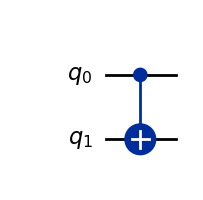
\includegraphics[width=0.3\textwidth]{Images/cnot-gate.png}
    \caption{CNOT Gate}
    \label{fig:cnot}
\end{figure}
Here it can be seen that the 1st Qubit is control and the 2nd Qubit is target. In the
figure \ref{fig:cnot}, the dot denotes the control qubit and the cross denotes the target qubit.

In the operator Notation it is:
\begin{align*}
    CX\ket{00}&=\ket{00} \\
    CX\ket{01}&=\ket{01} \\
    CX\ket{10}&=\ket{11} \\
    CX\ket{11}&=\ket{10}
\end{align*}
It is represented by the matrix in the computational basis ($\ket{00},\ket{01},\ket{10},\ket{11}$) as:
\[
    CX=\begin{bmatrix}
        1 & 0 & 0 & 0 \\
        0 & 1 & 0 & 0 \\
        0 & 0 & 0 & 1 \\
        0 & 0 & 1 & 0
    \end{bmatrix}
\]
In Outer product representation, it can be written as:
\[
    CX=\ket{00}\bra{00}+\ket{01}\bra{01}+\ket{10}\bra{11}+\ket{11}\bra{10}
\]
In Compact form we can write the CNOT gate as:
\[
    CX\ket{x}\ket{y}=\ket{x}\ket{x\oplus y}
\]
where $\oplus$ denotes the XOR operation. If the control qubit is set to $\ket{1}$ then the target qubit is flipped, otherwise the target qubit is left alone. It is a non-linear operation and used in Quantum Error Correction Codes.
This is a very important gate which is used in Teleoprtation protocol, Superdense Coding, Quantum Error Correction Codes etc.
Action of CX/CNOT on general two - qubit $\ket{\psi} = \alpha\ket{00}+\beta\ket{01}+\gamma\ket{10}+\delta\ket{11}$ is:
\[
    \begin{bmatrix} 
        1 & 0 & 0 & 0 \\
        0 & 1 & 0 & 0 \\
        0 & 0 & 0 & 1 \\
        0 & 0 & 1 & 0
    \end{bmatrix}\begin{bmatrix}
        \alpha \\
        \beta \\
        \gamma \\
        \delta
    \end{bmatrix}=\begin{bmatrix}
        \alpha \\
        \beta \\
        \delta \\
        \gamma
    \end{bmatrix}=\alpha\ket{00}+\beta\ket{01}+\delta\ket{10}+\gamma\ket{11}
\]

\subsubsection{CY Gate}
It is a two qubit gate, also called as the Controlled-Y gate.
Here the 1st Qubit is controlled and the 2nd Qubit is target (Pauli - Y Gate)
(It is also possible in the other way that the 2nd Qubit is controlled and the 1st Qubit is target).

The truth table is as in table \ref{tab:cy}.
\begin{table}[ht]
    \centering
    \begin{tabular}{|c|c|c|}
        \hline
        Input & Output\\
        \hline
        $\ket{00}$ & $\ket{00}$\\
        $\ket{01}$   & $\ket{01}$\\
        $\ket{10}$   & $i\ket{10}$\\
        $\ket{11}$  & $-i\ket{11}$\\
        \hline
    \end{tabular}
    \caption{Truth Table for CY Gate}
    \label{tab:cy}
\end{table}
For the table in \ref{tab:cy}, the 1st Qubit is control and the 2nd Qubit is target.
Thus, the CY gate flips the target qubit if the control qubit is $\ket{1}$.
The code for the CY Gate is as follows:
\begin{lstlisting}[language=Python]
from qiskit import QuantumRegister, ClassicalRegister, QuantumCircuit
from numpy import pi

# Add 2 qubits for CNOT gate demo
qreg_q = QuantumRegister(2, 'q')
circuit = QuantumCircuit(qreg_q,name='CY Gate')

circuit.cy(qreg_q[0],qreg_q[1]) #Apply the CY gate

circuit.draw(output='mpl')#.savefig('../images/cy-gate.png') #Draw the circuit
\end{lstlisting}

The circuit symbol is as shown in figure \ref{fig:cy}.
\begin{figure}[ht]
    \centering
    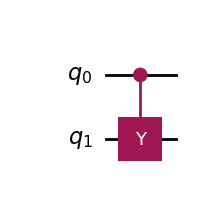
\includegraphics[width=0.3\textwidth]{Images/cy-gate.png}
    \caption{CY Gate}
    \label{fig:cy}
\end{figure}
In this figure \ref{fig:cy}, the first qubit is control and the second qubit is target.
If the first qubit is $\ket{1}$, then Y gate is applied on the second qubit. The Y Gate
is a gate which rotates the qubit by $\pi$ around the Y axis of Bloch Sphere. Thus, if
the input is $\ket{0}$, then the output is $\ket{0}$ and if the input is $\ket{1}$, then the output is $-i\ket{1}$.

In the operator Notation it is:
\begin{align*}
    CY\ket{00}&=\ket{00} \\
    CY\ket{01}&=\ket{01} \\
    CY\ket{10}&=i\ket{11} \\
    CY\ket{11}&=-i\ket{10}
\end{align*}
It is represented by the matrix in the computational basis ($\ket{00},\ket{01},\ket{10},\ket{11}$) as:
\[
    CY=\begin{bmatrix}
        1 & 0 & 0 & 0 \\
        0 & 1 & 0 & 0 \\
        0 & 0 & 0 & -\iota \\
        0 & 0 & \iota & 0
    \end{bmatrix}
\]
In Outer product representation, it can be written as:
\[
    CY=\ket{00}\bra{00}+\ket{01}\bra{01}+\iota\ket{11}\bra{10}-\iota\ket{10}\bra{11}
\]
In Compact form we can write the CY gate as:
\[
    CY\ket{xy}=(-1)^y\iota^x\ket{x(x\oplus y)}
\]
Flipping amplitude of 1 state. Marking of this state can be untilised for marking elements in data base.
It is useful in Grover's Algorithm.

Action of CY on general two - qubit $\ket{\psi} = \alpha\ket{00}+\beta\ket{01}+\gamma\ket{10}+\delta\ket{11}$ is:
\[
    \begin{bmatrix} 
        1 & 0 & 0 & 0 \\
        0 & 1 & 0 & 0 \\
        0 & 0 & 0 & -\iota \\
        0 & 0 & \iota & 0
    \end{bmatrix}\begin{bmatrix}
        \alpha \\
        \beta \\
        \gamma \\
        \delta
    \end{bmatrix}=\begin{bmatrix}
        \alpha \\
        \beta \\
        \iota\delta \\
        -\iota\gamma
    \end{bmatrix}=\alpha\ket{00}+\beta\ket{01}-\iota\delta\ket{10}+\iota\gamma\ket{11}
\]

\subsubsection{CZ/CPHASE Gate}
It is a two qubit gate, also called as the Controlled-Z gate.
Here the 1st Qubit is controlled and the 2nd Qubit is target (Pauli - Z Gate)
(It is also possible in the other way that the 2nd Qubit is controlled and the 1st Qubit is target).

The truth table is as in table \ref{tab:cz}.
\begin{table}[ht]
    \centering
    \begin{tabular}{|c|c|c|}
        \hline
        Input & Output\\
        \hline
        $\ket{00}$ & $\ket{00}$\\
        $\ket{01}$   & $\ket{01}$\\
        $\ket{10}$   & $\ket{10}$\\
        $\ket{11}$  & $-\ket{11}$\\
        \hline
    \end{tabular}
    \caption{Truth Table for CZ Gate}
    \label{tab:cz}
\end{table}
For the table in \ref{tab:cz}, the 1st Qubit is control and the 2nd Qubit is target.
Thus, the CZ gate flips the target qubit if the control qubit is $\ket{1}$.
The code for the CZ Gate is as follows:
\begin{lstlisting}[language=Python]
from qiskit import QuantumRegister, ClassicalRegister, QuantumCircuit
from numpy import pi

qreg_q = QuantumRegister(2, 'q')
circuit = QuantumCircuit(qreg_q,name='CZ Gate')

circuit.cz(qreg_q[0],qreg_q[1]) #Apply the CZ gate

circuit.draw(output='mpl')#.savefig('../images/CZ-gate.png') #Draw the circuit
\end{lstlisting}

The circuit symbol is as shown in figure \ref{fig:cz}.
\begin{figure}[ht]
    \centering
    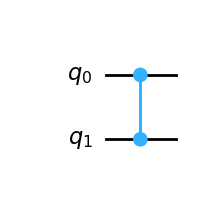
\includegraphics[width=0.3\textwidth]{Images/CZ-gate.png}
    \caption{CZ Gate}
    \label{fig:cz}
\end{figure}
In this figure \ref{fig:cz}, the first qubit is control and the second qubit is target.
If the first qubit is $\ket{1}$, then Z gate is applied on the second qubit. The Z Gate
is a gate which rotates the qubit by $\pi$ around the Z axis of Bloch Sphere. Thus, if 
the input is $\ket{0}$, then the output is $\ket{0}$ and if the input is $\ket{1}$, then the output is $-\ket{1}$.

In the operator Notation it is:
\begin{align*}
    CZ\ket{00}&=\ket{00} \\
    CZ\ket{01}&=\ket{01} \\
    CZ\ket{10}&=\ket{10} \\
    CZ\ket{11}&=-\ket{11}
\end{align*}
It is represented by the matrix in the computational basis ($\ket{00},\ket{01},\ket{10},\ket{11}$) as:
\[
    CZ=\begin{bmatrix}
        1 & 0 & 0 & 0 \\
        0 & 1 & 0 & 0 \\
        0 & 0 & 1 & 0 \\
        0 & 0 & 0 & -1
    \end{bmatrix}
\]
In Outer product representation, it can be written as:
\[
    CZ=\ket{00}\bra{00}+\ket{01}\bra{01}+\ket{10}\bra{10}-\ket{11}\bra{11}
\]
In Compact form we can write the CZ gate as:
\[
    CZ\ket{xy}=(-1)^{xy}\ket{xy}
\]

Action of CZ on general two - qubit $\ket{\psi} = \alpha\ket{00}+\beta\ket{01}+\gamma\ket{10}+\delta\ket{11}$ is:
\[
    \begin{bmatrix} 
        1 & 0 & 0 & 0 \\
        0 & 1 & 0 & 0 \\
        0 & 0 & 1 & 0 \\
        0 & 0 & 0 & -1
    \end{bmatrix}\begin{bmatrix}
        \alpha \\
        \beta \\
        \gamma \\
        \delta
    \end{bmatrix}=\begin{bmatrix}
        \alpha \\
        \beta \\
        \gamma \\
        -\delta
    \end{bmatrix}=\alpha\ket{00}+\beta\ket{01}+\gamma\ket{10}-\delta\ket{11}
\]

\subsubsection{CH/ Controlled Hadamard Gate}
It is a two qubit gate, also called as the Controlled-Hadamard gate.
Here the 1st Qubit is controlled and the 2nd Qubit is target.
The truth table is as in table \ref{tab:ch}.
\begin{table}[ht]
    \centering
    \begin{tabular}{|c|c|c|}
        \hline
        Input & Output\\
        \hline
        $\ket{00}$ & $\ket{00}$\\
        $\ket{01}$   & $\ket{01}$\\
        $\ket{10}$   & $\frac{1}{\sqrt{2}}(\ket{10}+\ket{11})$\\
        $\ket{11}$  & $\frac{1}{\sqrt{2}}(\ket{10}-\ket{11})$\\
        \hline
    \end{tabular}
    \caption{Truth Table for CH Gate}
    \label{tab:ch}
\end{table}
For the table in \ref{tab:ch}, the 1st Qubit is control and the 2nd Qubit is target.
Thus, the CH gate applies Hadamard gate on the target qubit if the control qubit is $\ket{1}$.
The code for the CH Gate is as follows:
\begin{lstlisting}[language=Python]
from qiskit import QuantumRegister, ClassicalRegister, QuantumCircuit
from numpy import pi

# Add 2 qubits for CNOT gate demo
qreg_q = QuantumRegister(2, 'q')
circuit = QuantumCircuit(qreg_q,name='CY Gate')

circuit.ch(qreg_q[0],qreg_q[1]) #Apply the CH gate

circuit.draw(output='mpl')#.savefig('../images/ch-gate.png') #Draw the circuit
\end{lstlisting}

The circuit symbol is as shown in figure \ref{fig:ch}.
\begin{figure}[ht]
    \centering
    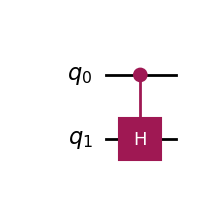
\includegraphics[width=0.3\textwidth]{Images/ch-gate.png}
    \caption{CH Gate}
    \label{fig:ch}
\end{figure}
In this figure \ref{fig:ch}, the first qubit is control and the second qubit is target.
If the first qubit is $\ket{1}$, then Hadamard gate is applied on the second qubit. The Hadamard Gate
is a gate which rotates the qubit by $\pi$ around the X axis of Bloch Sphere. Thus, if
the input is $\ket{0}$, then the output is $\ket{0}$ and if the input is $\ket{1}$, then the output is $\frac{1}{\sqrt{2}}(\ket{0}+\ket{1})$.

In the operator Notation it is:
\begin{align*}
    CH\ket{00}&=\ket{00} \\
    CH\ket{01}&=\ket{01} \\
    CH\ket{10}&=\frac{1}{\sqrt{2}}(\ket{10}+\ket{11}) \\
    CH\ket{11}&=\frac{1}{\sqrt{2}}(\ket{10}-\ket{11})
\end{align*}
It is represented by the matrix in the computational basis ($\ket{00},\ket{01},\ket{10},\ket{11}$) as:
\[
    CH=\begin{bmatrix}
        1 & 0 & 0 & 0 \\
        0 & 1 & 0 & 0 \\
        0 & 0 & \frac{1}{\sqrt{2}} & \frac{1}{\sqrt{2}} \\
        0 & 0 & \frac{1}{\sqrt{2}} & -\frac{1}{\sqrt{2}}
    \end{bmatrix}
\]
In Outer product representation, it can be written as:
\[
    CH=\ket{00}\bra{00}+\ket{01}\bra{01}+\frac{1}{\sqrt{2}}\ket{10}\bra{10}+\frac{1}{\sqrt{2}}\ket{10}\bra{11}
\]
In Compact form we can write the CH gate as:
\[
    CH\ket{xy}=\left(\frac{1}{\sqrt{2}}\right)^x\left(\ket{x(x\oplus y)}+(-1)^y\ket{xy}\right)
\]

Action of CH on general two - qubit $\ket{\psi} = \alpha\ket{00}+\beta\ket{01}+\gamma\ket{10}+\delta\ket{11}$ is:
\[
    \begin{bmatrix} 
        1 & 0 & 0 & 0 \\
        0 & 1 & 0 & 0 \\
        0 & 0 & \frac{1}{\sqrt{2}} & \frac{1}{\sqrt{2}} \\
        0 & 0 & \frac{1}{\sqrt{2}} & -\frac{1}{\sqrt{2}}
    \end{bmatrix}\begin{bmatrix}
        \alpha \\
        \beta \\
        \gamma \\
        \delta
    \end{bmatrix}=\begin{bmatrix}
        \alpha \\
        \beta \\
        \frac{\gamma+\delta}{\sqrt{2}} \\
        \frac{\gamma-\delta}{\sqrt{2}}
    \end{bmatrix}=\alpha\ket{00}+\beta\ket{01}+\frac{\gamma+\delta}{\sqrt{2}}\ket{10}+\frac{\gamma-\delta}{\sqrt{2}}\ket{11}
\]

\begin{importantnote}
    The CX/CNOT, CY, CZ and CH gates are Unitary as well as Hermitian. In, general we can write any of the controlled gates where the first qubit acts as a control bit
    and the second qubit acts as a target bit in matrix form as show:
    \[
        \begin{bmatrix}
            I & 0 \\
            0 & U
        \end{bmatrix}
    \]
    where $I$ is the Identity matrix of size $2(2^{n-1}-1)\times 2(2^{n-1}-1)$ and $U$ is the Unitary matrix of size $2\times 2$. Now for forming any of the n-qubit control gates where 
    there are n-1 control bits and 1 target bit we replace U with the corresponding gate wich we wish to form. 
    For example, for 2-qubit Control Hadamard gate we replace U with the Hadamard gate matrix.
    \[
        \begin{bmatrix}
            I & 0 \\
            0 & H
        \end{bmatrix}
    \]
    Similarly, for any n-qubit control gate we can form the matrix by replacing U with the corresponding gate matrix.
    For example, for 3-qubit control Z gate we replace U with the Z gate matrix.
    \[
        \begin{bmatrix}
            I & 0 \\
            0 & Z
        \end{bmatrix}
    \]
    where I is the Identity matrix of size $6\times 6$ and Z is the Pauli-Z gate matrix of size $2 \times 2$.
    We will later on use this concept to create the CCNOT/Toffoli gate.

    More generally, suppose $U$ is an arbitrary single qubit unitary operation. A controlled-$U$ operation is a two qubit operation, again with a control and a target qubit. If the control qubit is set then $U$ is applied to the target qubit, otherwise the target qubit is left alone; that is, $\ket{c}\ket{t}\rightarrow \ket{c}U^c\ket{t}$. The controlled-$U$ operation is represented by the circuit shown in figure \ref{fig:cu}.
\end{importantnote}
\begin{figure}
        \centering
        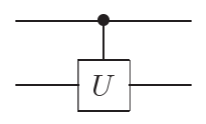
\includegraphics[width=0.25\linewidth]{Images/cu.png}
        \caption{Controlled-$U$ operation. The top line is the control qubit, and the bottom line is the target qubit. If the control qubit is set then $U$ is applied to the target, otherwise it is left alone.}
        \label{fig:cu}
    \end{figure}
\begin{example}
    \textbf{(Matrix representation of multi-qubit gates)}What is the $4\times 4$ unitary matrix for the circuit.
\begin{figure}[ht]
    \centering
    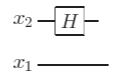
\includegraphics[width=0.25\linewidth]{Images/chexamp.png}
\end{figure}
in the computational basis? What is the unitary matrix for the circuit
\begin{figure}[ht]
    \centering
    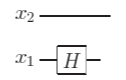
\includegraphics[width=0.25\linewidth]{Images/chexamp2.png}
\end{figure}
    in the computational basis?
Depending upon how the input bits are written as $x_1x_2$ or $x_2x_1$, we can write the matrix in different ways. Say as given in the question we first write $x_1$ and then $x_2$ then the following is the answer:\\
The unitary matrix for the first circuit is given by:
\[
I_1 \otimes H_2 = \begin{bmatrix} 1 & 0 \\ 0 & 1 \end{bmatrix} \otimes \frac{1}{\sqrt{2}}\begin{bmatrix} 1 & 1 \\ 1 & -1 \end{bmatrix} = \frac{1}{\sqrt{2}}\begin{bmatrix} 1 & 1 & 0 & 0 \\ 1 & -1 & 0 & 0 \\ 0 & 0 & 1 & 1 \\ 0 & 0 & 1 & -1 \end{bmatrix}
\]
The unitary matrix for the second circuit is given by:
\[
H_1 \otimes I_2 = \frac{1}{\sqrt{2}}\begin{bmatrix} 1 & 1 \\ 1 & -1 \end{bmatrix}\otimes \begin{bmatrix} 1 & 0 \\ 0 & 1 \end{bmatrix} = \frac{1}{\sqrt{2}} \begin{bmatrix} 1 & 0 & 1 & 0 \\ 0 & 1 & 0 & 1 \\ 1 & 0 & -1 & 0 \\ 0 & 1 & 1 &-1 \end{bmatrix}
\]
\end{example}

\begin{example}
    \textbf{(Building a CNOT from controlled-$Z$ gates)} Construct a CNOT gate from one controlled-$Z$ gate, that is, the gate whose action in the computational basis is specified by the unitary matrix
    \[
    \begin{bmatrix} 1 & 0 & 0 & 0 \\ 0 & 1 & 0 & 0 \\ 0 & 0 & 1 & 0 \\ 0 & 0 & 0 & -1 \end{bmatrix}
    \]
    and two Hadamard gates, specifying the control and target qubits.

    Recall that, $HZH=X$. Hence, to obtain a CNOT gate from a single controlled $Z$ gate, we can conjugate the target qubit with Hadamard gates:
    \begin{figure}[ht]
        \centering
        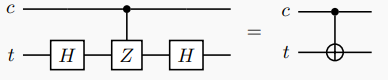
\includegraphics[width=0.5\linewidth]{Images/cnot-z.png}
    \end{figure}
    we can verify this via matrix multiplication, using the result from the previous example:
    \begin{align*}
        (I_1 \otimes H_2)(CZ_{12})(I_1\otimes H_2)&=\frac{1}{2}\begin{bmatrix} 1 & 1 & 0 & 0 \\ 1 & -1 & 0 & 0 \\ 0 & 0 & 1 & 1 \\ 0 & 0 & 1 & -1 \end{bmatrix}\begin{bmatrix} 1 & 0 & 0 & 0\\ 0 & 1 & 0 & 0 \\ 0 & 0 & 1 & 0 \\ 0 & 0 & 0 & -1 \end{bmatrix}\begin{bmatrix} 1 & 1 & 0 & 0 \\ 1 & -1 & 0 & 0 \\ 0 & 0 & 1 & 1 \\ 0 & 0 & 1 & -1 \end{bmatrix}\\
        &=\frac{1}{2}\begin{bmatrix} 2 & 0 & 0 & 0 \\ 0 & 2 & 0 & 0 \\ 0 & 0& 0 &  2\\ 0 & 0 & 2 & 0 \end{bmatrix}\\
        &=CX_{12}
    \end{align*}
\end{example}
\begin{example}
    Show that
    \begin{figure}[ht]
        \centering
        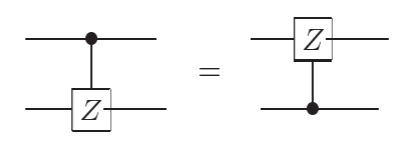
\includegraphics[width=0.5\linewidth]{Images/czzc.png}
    \end{figure}

    Recall that, we can write a controlled-$U$ operation as $CZ\ket{b_1}\ket{b_2} = \ket{b_1}\otimes Z^{b_1}\ket{b_2} = (-1)^{b_1 \cdot b_2} \ket{b_1}\ket{b_2}$ for computational basis states $b_1,b_2\in \{0,1\}$.

    Using this form we can write:
    \begin{align*}
        CZ_{12}\ket{b_1}\ket{b_2} &= (-1)^{b_1\cdot b_2} \ket{b_1}\ket{b_2}\\
        &=(-1)^{b_1\cdot b_2}\ket{b_1}\ket{b_2}\\
        &=Z^{b_2}\ket{b_1}\otimes \ket{b_2}\\
        &=CZ_{21}\ket{b_1}\ket{b_2}
    \end{align*}
    We can also verify this in other ways such as by seeing the action of the controlled gate on all the possible input qubits will be the same.
\end{example}

\begin{example}
    \textbf{(CNOT action on density matrices)} The CNOT gate is a simple permutation whose action on a density matrix $\rho$ is to rearrange the elements in the matrix. Write out this action explicitly in the computational basis.

    Let $\rho$ be an arbitrary density matrix corresponding to a $2$ qubit state. In the computational basis, we can write $\rho$ as:
    \[
    \rho = \begin{bmatrix} a_{11} & a_{12} & a_{12} & a_{14} \\ a_{21} & a_{22} & a_{23} & a_{24} \\ a_{31} & a_{32} & a_{33} & a_{34}\\a_{41} & a-{42} & a_{43} & a_{44} \end{bmatrix}
    \]
    Studying the action of the CNOT gate on this density matrix, we calculate:
    \begin{align*}
        CX_{12}\rho CX_{12} &=\begin{bmatrix} 1 & 0 & 0 & 0 \\ 0 & 1 & 0 & 0 \\ 0 & 0 & 0 & 1 \\ 0 & 0 & 1 & 0 \end{bmatrix} \begin{bmatrix} a_{11} & a_{12} & a_{13} & a_{14} \\ a_{21} & a_{22} & a_{23} & a_{24} \\ a_{31} & a_{32} & a_{33} & a_{34} \\ a_{41} & a_{42} & a_{43} & a_{44} \end{bmatrix}\begin{bmatrix} 1 & 0 & 0 & 0 \\ 0 & 1 & 0 & 0 \\ 0 & 0 & 0 & 1 \\ 0 & 0 & 1 & 0 \end{bmatrix}\\
        &=\begin{bmatrix} a_{11} & a_{12} & a_{13} & a_{14} \\ a_{21} & a_{22} & a_{23} & a_{24} \\ a_{41} & a_{42} & a_{43} & a_{44}\\ a_{31} & a_{32} & a_{33} & a_{34}  \end{bmatrix}\begin{bmatrix} 1 & 0 & 0 & 0 \\ 0 & 1 & 0 & 0 \\ 0 & 0 & 0 & 1 \\ 0 & 0 & 1 & 0 \end{bmatrix}\\
        &=\begin{bmatrix} a_{11} & a_{12} & a_{14} & a_{13}  \\ a_{21} & a_{22} & a_{24} & a_{23}  \\ a_{41} & a_{42}  & a_{44} & a_{43}\\ a_{31} & a_{32} & a_{34} & a_{33}  \end{bmatrix}
    \end{align*}
    Thus, the action of CNOT on density matrices is to rearrange the elements in the matrix as can be seen from the result.
\end{example}

\begin{example}
    \textbf{(CNOT basis transformations)} Unlike ideal classical gates ideal quantum gates do not have (as electrical engineers say)`high impedance' inputs. In fact, the role of `control' and `target' are arbitrary -they depend on what basis you think of a devices as operating in. We have described how CNOT behaves with respect to the computational basis, and in this description the state of the control qubit is not changed. However, if we work in a different basis then the control qubit does change: we will show that its phase is flipped depending on the state of the target qubit! Show that
    \begin{figure}[ht]
        \centering
        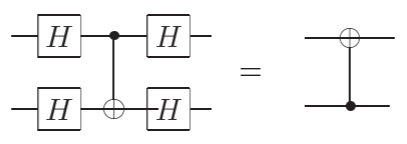
\includegraphics[width=0.5\linewidth]{Images/exampimg.png}
    \end{figure}
    using the identity from the previous example that $CX=(I_1\otimes H_2)(CZ_{12})(I_1\otimes H_2)$, and $CZ_{12}=CZ_{21}$, we get,
    \begin{align*}
        (H\otimes H)(CX_{12})(H\otimes H)&=(H\otimes H)(I\otimes H)(CZ_{12})(I\otimes H)(H\otimes H)\\
        &=(H\otimes I)(CZ_{12})(H\otimes I)\\
        &=(H\otimes I)CZ_{21}(H\otimes I)\\
        &=CX_{21}
    \end{align*}
    which proves the circuit identity. We know already that $CX\ket{c}\ket{t}=\ket{c}\ket{c\oplus t}$. So using the proven identity and the fact that $H\ket{0}=\ket{+},H\ket{1}=\ket{-}$, we obtain the required map.
    Introducing basis states $\ket{\pm} \equiv (\ket{0}\pm\ket{1})/\sqrt{2}$, use this circuit identity to show that the effect of a CNOT with the first qubit as control and the second qubit as target is as follows:
    \begin{align*}
        \ket{+}\ket{+}&\rightarrow \ket{+}\ket{+}\\
        \ket{-}\ket{+}&\rightarrow \ket{-}\ket{+}\\
        \ket{+}\ket{-}&\rightarrow \ket{-}\ket{-}\\
        \ket{-}\ket{-}&\rightarrow \ket{+}\ket{-}
    \end{align*}
    Thus, with respect to this new basis, the state of the target qubit is not changed, while the state of the control qubit is flipped if the target starts as $ket{-}$, otherwise it is left alone. That is, in this basis, the target and control have essentially interchanged roles.
\end{example}
\subsubsection{SWAP Gate}
It is a two Qubit Gate which swaps the states of the two qubits.
The truth table is as in table \ref{tab:swap}.
\begin{table}[ht]
    \centering
    \begin{tabular}{|c|c|c|}
        \hline
        Input & Output\\
        \hline
        $\ket{00}$ & $\ket{00}$\\
        $\ket{01}$   & $\ket{10}$\\
        $\ket{10}$   & $\ket{01}$\\
        $\ket{11}$  & $\ket{11}$\\
        \hline
    \end{tabular}
    \caption{Truth Table for SWAP Gate}
    \label{tab:swap}
\end{table}
The code for the SWAP Gate is as follows:
\begin{lstlisting}[language=Python]
from qiskit import QuantumRegister, ClassicalRegister, QuantumCircuit
from numpy import pi

# Add 2 qubits for CNOT gate demo
qreg_q = QuantumRegister(2, 'q')
circuit = QuantumCircuit(qreg_q,name='SWAP Gate')

circuit.swap(qreg_q[0],qreg_q[1]) #Apply the SWAP gate

circuit.draw(output='mpl')#.savefig('../images/swap-gate.png') #Draw the circuit
\end{lstlisting}

The circuit symbol is as shown in figure \ref{fig:swap}.
\begin{figure}[ht]
    \centering
    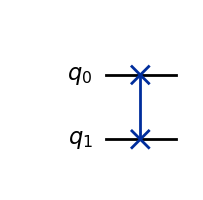
\includegraphics[width=0.3\textwidth]{Images/swap-gate.png}
    \caption{SWAP Gate}
    \label{fig:swap}
\end{figure}

In the operator Notation it is:
\begin{align*}
    SWAP\ket{00}&=\ket{00} \\
    SWAP\ket{01}&=\ket{10} \\
    SWAP\ket{10}&=\ket{01} \\
    SWAP\ket{11}&=\ket{11}
\end{align*}

It is represented by the matrix in the computational basis ($\ket{00},\ket{01},\ket{10},\ket{11}$) as:
\[
    SWAP=\begin{bmatrix}
        1 & 0 & 0 & 0 \\
        0 & 0 & 1 & 0 \\
        0 & 1 & 0 & 0 \\
        0 & 0 & 0 & 1
    \end{bmatrix}
\]
In Outer product representation, it can be written as:
\[
    SWAP=\ket{00}\bra{00}+\ket{01}\bra{10}+\ket{10}\bra{01}+\ket{11}\bra{11}
\]

Action of SWAP on general two - qubit $\ket{\psi} = \alpha\ket{00}+\beta\ket{01}+\gamma\ket{10}+\delta\ket{11}$ is:
\[
    \begin{bmatrix} 
        1 & 0 & 0 & 0 \\
        0 & 0 & 1 & 0 \\
        0 & 1 & 0 & 0 \\
        0 & 0 & 0 & 1
    \end{bmatrix}\begin{bmatrix}
        \alpha \\
        \beta \\
        \gamma \\
        \delta
    \end{bmatrix}=\begin{bmatrix}
        \alpha \\
        \gamma \\
        \beta \\
        \delta
    \end{bmatrix}=\alpha\ket{00}+\gamma\ket{01}+\beta\ket{10}+\delta\ket{11}
\]

SWAP Gate can also be formed using CNOT gates as follows:
\begin{figure}[ht]
    \centering
    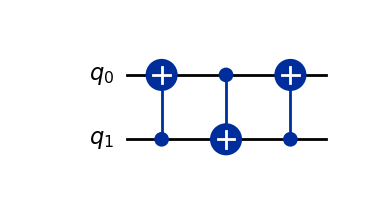
\includegraphics[width=0.3\textwidth]{Images/swap-gatemeth1.png}
    \caption{SWAP Gate using CNOT Gates}
    \label{fig:swap-cnot1}
\end{figure}
Or using CNOT gates as follows:
\begin{figure}[ht]
    \centering
    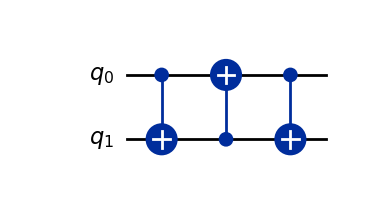
\includegraphics[width=0.3\textwidth]{Images/swap-gatemeth2.png}
    \caption{SWAP Gate using CNOT Gates}
    \label{fig:swap-cnot2}
\end{figure}

\begin{importantnote}
    The global phase does not matter provided we are doing a measurement at the end (or in between). If we are not doing any measurement then the global phase does matter in the computation.
\end{importantnote}



\subsection{Three-qubit Gates}
\subsubsection{CCNOT/Toffoli Gate}
It is a three qubit gate, also called as the CCNOT gate.
Here the 1st and 2nd Qubits are controlled and the 3rd Qubit is target.
The truth table is as in table \ref{tab:toffoli}.
\begin{table}[ht]
    \centering
    \begin{tabular}{|c|c|c|}
        \hline
        Input & Output\\
        \hline
        $\ket{000}$ & $\ket{000}$\\
        $\ket{001}$   & $\ket{001}$\\
        $\ket{010}$   & $\ket{010}$\\
        $\ket{011}$  & $\ket{011}$\\
        $\ket{100}$ & $\ket{100}$\\
        $\ket{101}$   & $\ket{101}$\\
        $\ket{110}$   & $\ket{111}$\\
        $\ket{111}$  & $\ket{110}$\\
        \hline
    \end{tabular}
    \caption{Truth Table for Toffoli Gate}
    \label{tab:toffoli}
\end{table}
For the table in \ref{tab:toffoli}, the 1st and 2nd Qubits are control and the 3rd Qubit is target.
Thus, the Toffoli gate flips the target qubit if the control qubits are $\ket{1}$.
The code for the Toffoli Gate is as follows:
\begin{lstlisting}[language=Python]
from qiskit import QuantumRegister, ClassicalRegister, QuantumCircuit
from numpy import pi

qreg_q = QuantumRegister(3, 'q')
circuit = QuantumCircuit(qreg_q)

circuit.ccx(qreg_q[0], qreg_q[1], qreg_q[2])

circuit.draw(output='mpl')#.savefig('../images/ccx-gate.png')
\end{lstlisting}

The circuit symbol is as shown in figure \ref{fig:toffoli}.
\begin{figure}[ht]
    \centering
    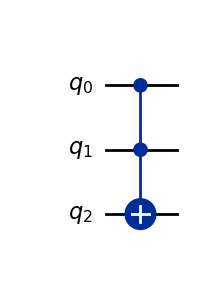
\includegraphics[width=0.3\textwidth]{Images/ccx-gate.png}
    \caption{Toffoli Gate}
    \label{fig:toffoli}
\end{figure}
In this figure \ref{fig:toffoli}, the first and second qubits are control and the third qubit is target.
If the first and second qubits are $\ket{1}$, then the third qubit is flipped. The Toffoli Gate
is a gate which flips the target qubit if the control qubits are $\ket{1}$.

In the operator Notation it is:
\begin{align*}
    CCX\ket{000}&=\ket{000} \\
    CCX\ket{001}&=\ket{001} \\
    CCX\ket{010}&=\ket{010} \\
    CCX\ket{011}&=\ket{011} \\
    CCX\ket{100}&=\ket{100} \\
    CCX\ket{101}&=\ket{101} \\
    CCX\ket{110}&=\ket{111} \\
    CCX\ket{111}&=\ket{110}
\end{align*}

It is represented by the matrix in the computational basis 
($\ket{000},\ket{001},\ldots,\ket{110},\ket{111}$) as:
\[
    CCX=\begin{bmatrix}
        1 & 0 & 0 & 0 & 0 & 0 & 0 & 0 \\
        0 & 1 & 0 & 0 & 0 & 0 & 0 & 0 \\
        0 & 0 & 1 & 0 & 0 & 0 & 0 & 0 \\
        0 & 0 & 0 & 1 & 0 & 0 & 0 & 0 \\
        0 & 0 & 0 & 0 & 1 & 0 & 0 & 0 \\
        0 & 0 & 0 & 0 & 0 & 1 & 0 & 0 \\
        0 & 0 & 0 & 0 & 0 & 0 & 0 & 1 \\
        0 & 0 & 0 & 0 & 0 & 0 & 1 & 0
    \end{bmatrix}
\]
In Outer product representation, it can be written as:
\begin{align*}
    CCX&=\ket{000}\bra{000}+\ket{001}\bra{001}+\ket{010}\bra{010}+\ket{011}\bra{011} \\
    &+\ket{100}\bra{100}+\ket{101}\bra{101}+\ket{110}\bra{111}+\ket{111}\bra{110}
\end{align*}

Action of CCX on general three - qubit $\ket{\psi} = \alpha\ket{000}+\beta\ket{001}+\gamma\ket{010}+\delta\ket{011}+\epsilon\ket{100}+\zeta\ket{101}+\eta\ket{110}+\theta\ket{111}$ is:
\[
    \begin{bmatrix} 
        1 & 0 & 0 & 0 & 0 & 0 & 0 & 0 \\
        0 & 1 & 0 & 0 & 0 & 0 & 0 & 0 \\
        0 & 0 & 1 & 0 & 0 & 0 & 0 & 0 \\
        0 & 0 & 0 & 1 & 0 & 0 & 0 & 0 \\
        0 & 0 & 0 & 0 & 1 & 0 & 0 & 0 \\
        0 & 0 & 0 & 0 & 0 & 1 & 0 & 0 \\
        0 & 0 & 0 & 0 & 0 & 0 & 0 & 1 \\
        0 & 0 & 0 & 0 & 0 & 0 & 1 & 0
    \end{bmatrix}\begin{bmatrix}
        \alpha \\
        \beta \\
        \gamma \\
        \delta \\
        \epsilon \\
        \zeta \\
        \eta \\
        \theta
    \end{bmatrix}=\begin{bmatrix}
        \alpha \\
        \beta \\
        \gamma \\
        \delta \\
        \epsilon \\
        \zeta \\
        \theta \\
        \eta
    \end{bmatrix}=\alpha\ket{000}+\beta\ket{001}+\ldots+\zeta\ket{101}+\theta\ket{110}+\eta\ket{111}
\]

\subsubsection{CSWAP/Fredkin Gate}\label{qgate:cswap}
It is a three qubit gate, also called as the CSWAP gate.
Here the 1st Qubit is control and the 2nd and 3rd Qubits are target.
The truth table is as in table \ref{tab:fredkin}.
\begin{table}[ht]
    \centering
    \begin{tabular}{|c|c|c|}
        \hline
        Input & Output\\
        \hline
        $\ket{000}$ & $\ket{000}$\\
        $\ket{001}$   & $\ket{001}$\\
        $\ket{010}$   & $\ket{010}$\\
        $\ket{011}$  & $\ket{011}$\\
        $\ket{100}$ & $\ket{100}$\\
        $\ket{101}$   & $\ket{110}$\\
        $\ket{110}$   & $\ket{101}$\\
        $\ket{111}$  & $\ket{111}$\\
        \hline
    \end{tabular}
    \caption{Truth Table for Fredkin Gate}
    \label{tab:fredkin}
\end{table}
For the table in \ref{tab:fredkin}, the 1st Qubit is control and the 2nd and 3rd Qubits are target.
Thus, the Fredkin gate swaps the states of the 2nd and 3rd qubits if the control qubit is $\ket{1}$.
The code for the Fredkin Gate is as follows:
\begin{lstlisting}[language=Python]
from qiskit import QuantumRegister, ClassicalRegister, QuantumCircuit
from numpy import pi

qreg_q = QuantumRegister(3, 'q')
circuit = QuantumCircuit(qreg_q)

circuit.cswap(qreg_q[0], qreg_q[2], qreg_q[1])

circuit.draw(output='mpl')#.savefig('../images/cswap-gate.png')
\end{lstlisting}

The circuit symbol is as shown in figure \ref{fig:fredkin}.
\begin{figure}[ht]
    \centering
    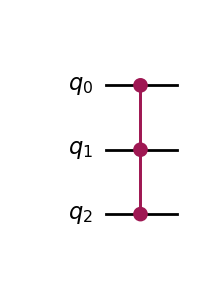
\includegraphics[width=0.3\textwidth]{Images/cswap-gate.png}
    \caption{Fredkin Gate}
    \label{fig:fredkin}
\end{figure}
In this figure \ref{fig:fredkin}, the first qubit is control and the second and third qubits are target.
If the first qubit is $\ket{1}$, then the second and third qubits are swapped. The Fredkin Gate
is a gate which swaps the states of the 2nd and 3rd qubits if the control qubit is $\ket{1}$.

In the operator Notation it is:
\begin{align*}
    CSWAP\ket{000}&=\ket{000} \\
    CSWAP\ket{001}&=\ket{001} \\
    CSWAP\ket{010}&=\ket{010} \\
    CSWAP\ket{011}&=\ket{011} \\
    CSWAP\ket{100}&=\ket{100} \\
    CSWAP\ket{101}&=\ket{110} \\
    CSWAP\ket{110}&=\ket{101} \\
    CSWAP\ket{111}&=\ket{111}
\end{align*}

It is represented by the matrix in the computational basis ($\ket{000},\ket{001},\ldots,\ket{110},\ket{111}$) as:
\[
    CSWAP=\begin{bmatrix}
        1 & 0 & 0 & 0 & 0 & 0 & 0 & 0 \\
        0 & 1 & 0 & 0 & 0 & 0 & 0 & 0 \\
        0 & 0 & 1 & 0 & 0 & 0 & 0 & 0 \\
        0 & 0 & 0 & 1 & 0 & 0 & 0 & 0 \\
        0 & 0 & 0 & 0 & 1 & 0 & 0 & 0 \\
        0 & 0 & 0 & 0 & 0 & 0 & 1 & 0 \\
        0 & 0 & 0 & 0 & 0 & 1 & 0 & 0 \\
        0 & 0 & 0 & 0 & 0 & 0 & 0 & 1
    \end{bmatrix}
\]
In Outer product representation, it can be written as:
\begin{align*}
    CSWAP&=\ket{000}\bra{000}+\ket{001}\bra{001}+\ket{010}\bra{010}+\ket{011}\bra{011} \\
    &+\ket{100}\bra{100}+\ket{101}\bra{110}+\ket{110}\bra{101}+\ket{111}\bra{111}
\end{align*}

Action of CSWAP on general three - qubit $\ket{\psi} = \alpha\ket{000}+\beta\ket{001}+\gamma\ket{010}+\delta\ket{011}+\epsilon\ket{100}+\zeta\ket{101}+\eta\ket{110}+\theta\ket{111}$ is:
\[
    \begin{bmatrix} 
        1 & 0 & 0 & 0 & 0 & 0 & 0 & 0 \\
        0 & 1 & 0 & 0 & 0 & 0 & 0 & 0 \\
        0 & 0 & 1 & 0 & 0 & 0 & 0 & 0 \\
        0 & 0 & 0 & 1 & 0 & 0 & 0 & 0 \\
        0 & 0 & 0 & 0 & 1 & 0 & 0 & 0 \\
        0 & 0 & 0 & 0 & 0 & 0 & 1 & 0 \\
        0 & 0 & 0 & 0 & 0 & 1 & 0 & 0 \\
        0 & 0 & 0 & 0 & 0 & 0 & 0 & 1
    \end{bmatrix}\begin{bmatrix}
        \alpha \\
        \beta \\
        \gamma \\
        \delta \\
        \epsilon \\
        \zeta \\
        \eta \\
        \theta
    \end{bmatrix}=\begin{bmatrix}
        \alpha \\
        \beta \\
        \gamma \\
        \delta \\
        \epsilon \\
        \zeta \\
        \theta \\
        \eta
    \end{bmatrix}=\alpha\ket{000}+\beta\ket{001}+\ldots+\zeta\ket{101}+\theta\ket{110}+\eta\ket{111}
\]

We can construct Fredkin gate using CNOT and Toffoli gate as shown in the figure \ref{fig:fredkin-cnot1}.
\begin{figure}[ht]
    \centering
    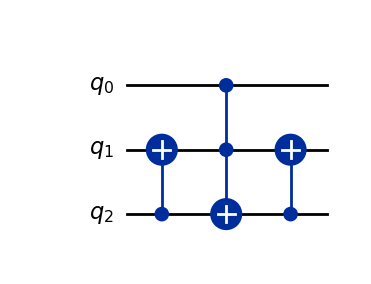
\includegraphics[width=0.3\textwidth]{Images/cswap-gatemeth1.png}
    \caption{Fredkin Gate using CNOT and Toffoli Gates}
    \label{fig:fredkin-cnot1}
\end{figure}

\begin{importantnote}
    Applying a gate on a superposition state is the same as applying the gate on each of the basis states and then superposing the results.
    This is because, the gate is a linear operator and the superposition is a linear combination of the basis states. 
    Thus, the gate can be applied on each of the basis states and then the results can be superposed. For example, Consider a superposition state $\ket{\psi}=\alpha\ket{0}+\beta\ket{1}$.
    If we apply a gate $U$ on this state, then the output will be $U\ket{\psi}=U(\alpha\ket{0}+\beta\ket{1})=\alpha U\ket{0}+\beta U\ket{1}$.
    Thus, the gate can be applied on each of the basis states and then the results can be superposed. This, can also be thought that since U is a $2 \times 2$ matrix and $\ket{0}$ and $\ket{1}$ are $2 \times 1$ column vectors, 
    multiplying $U(\alpha\ket{0}+\ket{1})$ is same as $\alpha U\ket{0}+\beta U\ket{1}$ Since Matrix multiplication is distributive. 

    For example, say CNOT gate needs to be applied on a superposition of two bits $\ket{\psi}=\alpha\ket{00}+\beta\ket{01}+\gamma\ket{10}+\delta\ket{11}$.
    Then the output will be $CNOT\ket{\psi}=CNOT(\frac{\ket{00}+\ket{11}}{\sqrt{2}})=\frac{CNOT\ket{00}+CNOT\ket{11}}{\sqrt{2}}$.
    which will thus be $\frac{\ket{00}+\ket{10}}{\sqrt{2}}$.
    In the matrix form, 
    \[
        CNOT\ket{\psi}=CNOT\left(\frac{\ket{00}+\ket{11}}{\sqrt{2}}\right)=\begin{bmatrix}
            1 & 0 & 0 & 0 \\
            0 & 1 & 0 & 0 \\
            0 & 0 & 0 & 1 \\
            0 & 0 & 1 & 0
        \end{bmatrix}\frac{1}{\sqrt{2}}\left(\begin{bmatrix}
            1 \\
            0 \\
            0 \\
            0
        \end{bmatrix}+\begin{bmatrix}
            0 \\
            0 \\
            0 \\
            1
        \end{bmatrix}\right)
    \]
    \[=\frac{1}{\sqrt{2}}\left(\begin{bmatrix}
        1 & 0 & 0 & 0 \\
        0 & 1 & 0 & 0 \\
        0 & 0 & 0 & 1 \\
        0 & 0 & 1 & 0
    \end{bmatrix}\begin{bmatrix}
        1 \\
        0 \\
        0 \\
        0
    \end{bmatrix}+\begin{bmatrix}
        1 & 0 & 0 & 0 \\
        0 & 1 & 0 & 0 \\
        0 & 0 & 0 & 1 \\
        0 & 0 & 1 & 0
    \end{bmatrix}\begin{bmatrix}
        0 \\
        0 \\
        0 \\
        1
    \end{bmatrix}\right)
    \]
    \[
    =(CNOT\frac{1}{\sqrt{2}}\ket{00}+CNOT\frac{1}{\sqrt{2}}\ket{11})=\frac{1}{\sqrt{2}}CNOT\ket{00}+\frac{1}{\sqrt{2}}CNOT\ket{11}
    \]
    \[
        =\frac{1}{\sqrt{2}}\left(\begin{bmatrix}
            1 \\
            0 \\
            0 \\
            0
        \end{bmatrix}+\begin{bmatrix}
            0 \\
            0 \\
            1 \\
            0
        \end{bmatrix}\right)=\frac{1}{\sqrt{2}}\begin{bmatrix} 1 \\ 0 \\ 1 \\ 0 \end{bmatrix} =\frac{1}{\sqrt{2}}\left(\ket{00}+\ket{10}\right)
    \]
    Thus, applying a gate on a superposition is the same as applying the gate on the basis states of the superposition. Thus, the gate can be applied on each of the basis states and then the results can be superposed
    in the same linear combination as that in which the state $\ket{\psi}$ was superposed.
\end{importantnote}

\section{Implementation of Controlled-U}
Now we are required to understand how to implement the controlled-$U$ operation for arbitrary single qubit $U$, using only single qubit operations and the CNOT gate. Our strategy is a two-part procedure based upon the decomposition $e^{\iota\alpha}AXBXC$.

The first step will be to apply the phase shift exp($\iota\alpha$) on the target qubit, controlled by the control qubit. that is, if the control qubit is $\ket{0}$, then the target qubit is left alone, while if the control qubit is $\ket{1}$, a phase shift $e^{\iota\alpha}$ is applied to the target. A circuit implementing this operation using just a single qubit unitary gate is depicted as in the figure \ref{fig:unicontrolu}. to verify this circuit works correctly, note that the effect of the circuit on the right hand side is
\[
\ket{00}\rightarrow \ket{00},\quad \ket{01}\rightarrow \ket{01},\quad \ket{10}\rightarrow e^{\iota\alpha}\ket{10},\quad \ket{11}\rightarrow e^{\iota\alpha}\ket{11}
\]
\begin{figure}[ht]
    \centering
    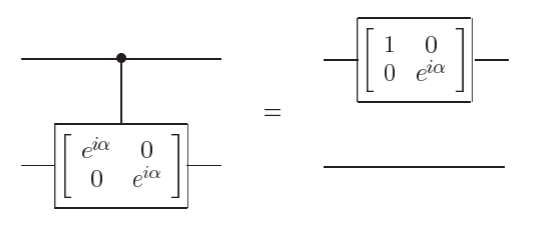
\includegraphics[width=0.5\linewidth]{Images/uncontrolu.png}
    \caption{Controlled phase shift gate and an equivalent circuit for two qubits}
    \label{fig:unicontrolu}
\end{figure}

We can now complete the construction of the controlled-U operation, as shown in figure \ref{fig:univcontrlledu}. to understand why this circuit works, recall that $U$ may be written in the form $U=e^{\iota\alpha}AXBXC$, where $A,B$ and $C$ are single qubit operations such that $ABC=I$. Suppose that the control qubit is set. then the operation $e^{\iota\alpha}AXBXC=U$ is applied to the second qubit. If, on the other hand, the control qubit is not set, then the operation $ABC=I$ is applied to the second qubit; that is, no change is made. That is, the circuit implements the controlled-$U$ operation.
\begin{figure}[ht]
    \centering
    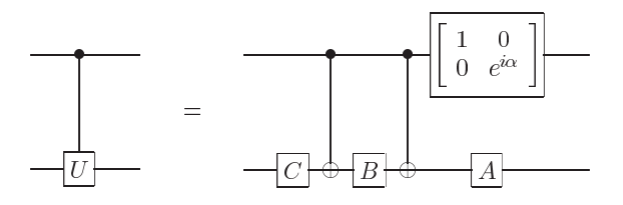
\includegraphics[width=0.5\linewidth]{Images/univcontrolledu.png}
    \caption{Circuit implementing the controlled-U operation for single qubit $U$. $\alpha,A,B$ and $C$ satisfy $U=exp(\iota\alpha) AXBXC, ABC=I$}
    \label{fig:univcontrlledu}
\end{figure}
now that we know how the condition on a single qubit set, what about conditioning on multiple qubits? We've already met one example of multiple qubit conditioning, the Toffoli gate, which flips the third qubit, the target qubit, conditioned on the first two qubits, the control qubits, being set to one. More generally, suppose we have $n+k$ qubits, and $U$ is a $k$ qubit unitary operator. Then we define the controlled operation $C^n(U)$ by the equation.
\[
C^n(U)\ket{x_1x_2\ldots x_n} \ket{\psi} = \ket{x_1x_2\ldots x_n}\ket{\psi}
\]
where $x_1x_2,\ldots x_n$ in the exponent of $U$ means the product of the bits $x_1,x_2,\ldots,x_n$. That is, the operator $U$ is applied to the last $k$ qubits if the first $n$ qubits are equal to one, and otherwise, nothing is done. Such conditional operations are so useful that we introduce a special circuit notation for them, illustrated in figure \ref{fig:multicontrolu}. For the following we assume that $k=1$, for simplicity. larger $k$ can be dealt with using essentially the same methods, however for $k\geq 2$ there is the added complication that we don't know how to perform arbitrary operations on $k$ qubits.
\begin{figure}
    \centering
    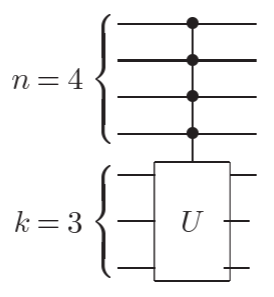
\includegraphics[width=0.25\linewidth]{Images/multicontrolu.png}
    \caption{Sample circuit representation for the $C^n(U)$ operation, where $U$ is a unitary operator on $k$ qubits, for $n=4$ and $k=3$.}
    \label{fig:multicontrolu}
\end{figure}
Suppose $U$ is a single qubit unitary operator, and $V$ is a unitary operator chosen so that $V^2=U$. Then the operation $C^2(U)$ may be implemented using the circuit shown in figure \ref{fig:controlv}.
\begin{figure}
    \centering
    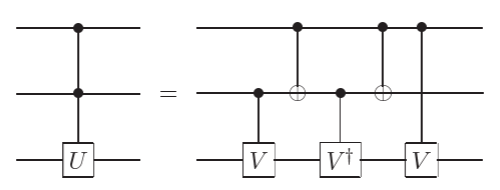
\includegraphics[width=0.75\linewidth]{Images/controlv.png}
    \caption{Circuit for the $C^2(U)$ gate. $V$ is any unitary operator satisfying $V^2=U$. The special case $V\equiv (1-\iota)(I+\iota X)/2$ corresponds to the Toffoli gate.}
    \label{fig:controlv}
\end{figure}
\begin{example}
    Verify that figure \ref{fig:controlv} implements the $C^2(U)$ operation.

    Considering all the possible inputs (in the computational basis) let us see the outcome for both the circuits. 
    \begin{align*}
        \ket{00\psi} &\rightarrow \ket{00\psi}\rightarrow \ket{00\psi}\rightarrow \ket{00\psi}\rightarrow \ket{00\psi}\rightarrow \ket{00\psi}\\
        \ket{01\psi}&\rightarrow \ket{01(V\psi)} \rightarrow \ket{01(V\psi)} \rightarrow \ket{01(V^{\dagger}V\psi)}\rightarrow\ket{01(V^{\dagger}V\psi)}\rightarrow \ket{01(V^{\dagger}V\psi)} = \ket{01\psi}\\
        \ket{10\psi}&\rightarrow \ket{10\psi}\rightarrow \ket{11\psi} \rightarrow \ket{11(V^{\dagger}\psi)} \rightarrow \ket{10(V^{\dagger}\psi)}\rightarrow \ket{10(VV^{\dagger}\psi)} = \ket{10\psi}\\
        \ket{11\psi} &\rightarrow \ket{11(V\psi)} \rightarrow \ket{10(V\psi)} \rightarrow \ket{10(V\psi)} \rightarrow \ket{11(V\psi)} \rightarrow\ket{11(V^2\psi)} = \ket{11(U\psi)}
    \end{align*}
    Hence, the circuit does perform the $C^2(U)$ operation.
\end{example} 

\begin{example}
    Prove that a $C^2(U)$ gate (for any single qubit unitary $U$) can be constructed using at most eight one-qubit gates, and six controlled-NOTs.
    Firstly, we apply the circuit if figure \ref{fig:multicontrolu} to the circuit in figure \ref{fig:controlv} which gives,
    \begin{figure}[ht]
        \centering
        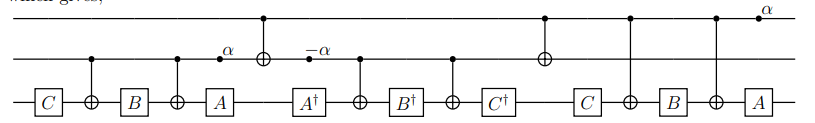
\includegraphics[width=1\linewidth]{Images/c2uimpl.png}
    \end{figure}
    We move the 6th CNOT left from the 4th one, which involves adding CNOTs after the 4th and 5th CNOTs from first to third qubit, which is due to,
    \begin{figure}[ht]
        \centering
        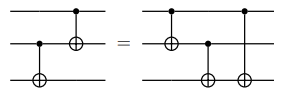
\includegraphics[width=0.5\linewidth]{Images/c2uimpl2.png}
    \end{figure}
    and can be checked by consider all the possible inputs. We also see that $AA^{\dagger}=CC^{\dagger}=I$. Hence, we get the following circuit.
    \begin{figure}[ht]
        \centering
        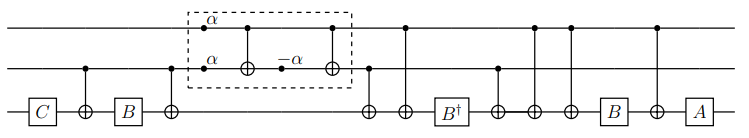
\includegraphics[width=1\linewidth]{Images/c2uimpl3.png}
    \end{figure}
    The dashed is diagonal hence commutes with the rest of the components therefore can be moved to the end for convenience.
    \begin{figure}[ht]
        \centering
        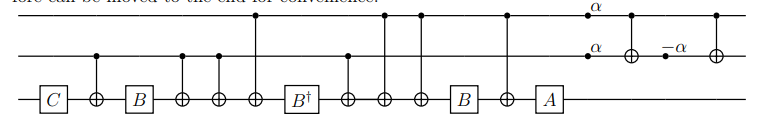
\includegraphics[width=1\linewidth]{Images/c2uimpl4.png}
    \end{figure}
    CNOTs 2 and 3, 6 and 7 cancel each other, hence we are left with the circuit 
    This has $8$ single qubit gates and $6$ CNOTs as desired. The circuit performs the operation, $AXBXB^{\dagger}XBXC=(VC^{\dagger})B^{\dagger}(A^{\dagger}V)=V^2 = U$. Therefore, the circuit performs the $C^2(U)$ operation.
\end{example}

\begin{example} 
Construct a $C^1(U)$ gate for $U=R_x(\theta)$ and $U=R_y(\theta)$, using only CNOT and single qubit gates. Can you reduce the number of single qubit gates need in the construction from three to two?
\end{example}

The familiar Toffoli gate is an especially important special case of $C^2(U)$ operation , the case $C^2(X)$. Defining $V(1-\iota)(I_\iota X)/2$ and noting that $V^2=X$, we see that figure \ref{fig:c2utoff} gives an implementation of the Toffoli gate in terms of one and two qubit operations. From a classical viewpoint this is a remarkable result. Recall that one and two bit classical reversible gates are not sufficient to implement the Toffoli gate, or more generally, universal computation. By contrast, in the quantum case we see that one and two qubit reversible gates are sufficient to implement the Toffoli gate, and will eventually prove that they suffice for universal computation. 
\begin{figure}[ht]
    \centering
    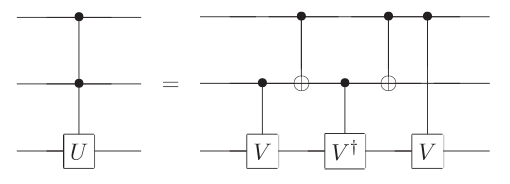
\includegraphics[width=0.75\linewidth]{Images/c2Utoffoli.png}
    \caption{Circuit for the $C^2(U)$ gate. $V$ is any unitary operator satisfying $ V^2=U$. The special case $V=(1-\iota)(I+\iota X)/2$ corresponds to the Toffoli gate.}
    \label{fig:c2utoff}
\end{figure}
Ultimately we will show that any unitary operation can be composed into an arbitrary good approximation from just the Hadamard, phase, controlled-NOT and $\pi/8$ gates. Because of the great usefulness of the Toffoli gate it is interesting to see how it can be built from just this gate set. Figure \ref{fig:toffdecomp} illustrates a simple circuit for the Toffoli gate made up of just Hadamard, phase, controlled-NOT and $pi/8$ gates.
\begin{figure}[ht]
    \centering
    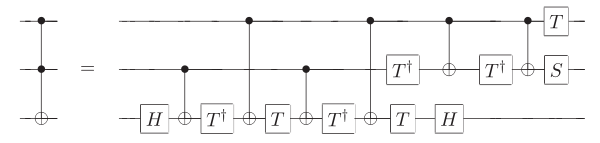
\includegraphics[width=1\linewidth]{Images/toffoli_decomp.png}
    \caption{Implementation of the Toffoli gate using Hadamard, phase, controlled-NOT and $\pi/8$ gates}
    \label{fig:toffdecomp}
\end{figure}

How may we implement $C^n(U)$ gates using our existing repertoire of gates where $U$ is an arbitrary single qubit unitary operation? A particularly simple circuit for achieving this task is illustrated in figure \ref{fig:controlnu}. The circuit divides up into three stages and makes use of a small number $(n-1)$ working qubits, which all start and end in the state $\ket{0}$. Suppose the control qubits are in the computational basis state $\ket{c_1,c_2,\ldots,c_n}$. The first stage of the circuit is to reversible ANd all the control bits $c_1,\ldots,c_n$ together to produce the product $c)1\cdot c_2 \ldots c_n$. To do this, the first gate in the circuit ANDs $c_1$ and $c_2$ together, using a Toffoli gate, changing the state of the first work qubit to $\ket{c_1\cdot c_2}$. The next Toffoli gate ANDs $c_3$ with the product $c_1 \cdot c_2$, changing the state of the second work qubit to $\ket{c_1\cdot c_2 \cdot c_3}$. We continue applying Toffoli gates in this fashion, until the final work qubit is in the state $\ket{c_1 \cdot c_2\ldots c_n}$. Next, a $U$ operation on the target qubit is performed, conditional on the final work qubit being set to one. That is, $U$ is applied if and only if all of $c_1$ through $c_n$ are set. Finally, the last part of the circuit just reverses the steps of the first stage, returning all the work qubits to their initial state, $\ket{0}$. The combined result, therefore, is to apply the unitary operator $U$ to the target qubit, if and only if all the control bits $c_1$ through $c_n$ are set, as desired.
\begin{figure}[ht]
    \centering
    \includegraphics[width=1\linewidth]{Images/controlnu.png}
    \caption{Network implementing the $C^n(U)$ operation for the case, $n=5$}
    \label{fig:controlnu}
\end{figure}
In the controlled gates we have been considering, conditional dynamics on the target qubit occurs if the control bits are set to one. Of course, there is nothing special about one, and it is often useful to consider dynamics which occurs conditional on the control bits being set to zero. For instance, suppose we wish to implement a two qubit gate in which the second (`target') qubit is flipped, conditional on the first (`control') qubit being set to zero. In figure \ref{fig:controldecomp} we introduce a circuit notation for this gate, together with an equivalent circuit in terms of the gates we have already introduced. Generically we shall use the open circle notation to indicate condition on the qubit being set to zero, while a closed circle indicates conditioning on the qubit being set to one.
\begin{figure}[ht]
    \centering
    \includegraphics[width=1\linewidth]{Images/controlxdecomp.png}
    \caption{Controlled operation with a NOT gate being performed on the second qubit, conditional on the first qubit being set to zero}
    \label{fig:controldecomp}
\end{figure}
A more elaborate example of this connection, involving three control qubits, is illustrated in figure \ref{fig:cuequiv}. The operation $U$ is applied to the target qubit if the first and third qubits are set to zero, and the second qubit is set to one. It is easy to verify by inspection that the circuit on the right hand side of the figure implements the desired operation. More generally, it is easy to move between circuits which condition on qubits being set to one and circuit which condition on qubits being set to zero, by insertion of $X$ gates in appropriate locations, as illustrated in figure \ref{fig:cuequiv}.
\begin{figure}[ht]
    \centering
    \includegraphics[width=1\linewidth]{Images/cuequiv.png}
    \caption{Controlled-$U$ operation and its equivalent in terms of circuit elements we already know how to implement. The fourth qubit has $U$ applied if the first and third qubits are set to zero, and the second qubit is set to one.}
    \label{fig:cuequiv}
\end{figure}
Another convention which sometimes is useful is to allow the controlled-NOT gates to have multiple targets as shown in figure \ref{fig:multitargetcnot}. This natural notation means that when the control qubit is $1$, then all the qubits marked with a $\oplus$ are flipped, and otherwise nothing happens. It is convenient to use, for example, in construction classical functions such as permutations, or in encodes and decodes for quantum error-correction circuits, as we shall later see.
\begin{figure}[ht]
    \centering
    \includegraphics[width=0.5\linewidth]{Images/multiplegatescontrollednot.png}
    \caption{Controlled-NOT gate with multiple targets}
    \label{fig:multitargetcnot}
\end{figure}

\section{Universal quantum gates}
A small set of gates (e.g. AND, OR, NOT) can be used to compute an arbitrary classical functions. We say that such a set of gates is universal for classical computation. In fact, since the Toffoli gate is universal for classical computation, quantum circuits subsume classical circuits. A similar universality is true for quantum computation, where a set of gates is said to be universal for quantum computation if any unitary operation may be approximated to arbitrary accuracy by a quantum circuit involving only those gates. We now describe three universality constructions for quantum computation. These constructions build upon each other, and culminate a proof that any unitary operation can be approximated to arbitrary accuracy using Hadamard, phase, CNOT, and $\pi/8$ gates. You may wonder why the phase gate appears in this list, since it can be constructed from two $\pi/8$ gates; it is included because of its natural role in fault-tolerant constructions described later.

The first construction shows that any arbitrary unitary operator may be expressed exactly as a product of unitary operators that each acts non-trivially only on a subspace spanned by two computational basis states. The second construction combines the first construction with the results of the previous section to show that an arbitrary unitary operator may be expressed exactly using single qubit and CNOT gates. The third construction combines the second construction with a proof that single qubit operation may be approximated to arbitrary accuracy using the Hadamard, phase, and $\pi/8$ gates. This in turn implies that any unitary operation can be approximated to arbitrary accuracy using Hadamard, phase, CNOT and $\pi/8$ gates.

Our construction say little about efficiency - how many (polynomially or exponentially many) gates must be composed in order to create a given unitary transform. Later we show that there exist unitary transforms which require exponentially many gates to approximate. Of course, the goal of quantum computation is to find interesting families of unitary transformations that can be performed efficiently.

\begin{example}
    Construct a quantum circuit to add two two-bit numbers $x$ and $y$ modulo $4$. That is, the circuit should perform the transformation $\ket{x,y} \rightarrow \ket{x,x+y \text{ mod } 4}$.
\end{example}

\subsection{Two-level unitary gates are universal}
Consider a Unitary matrix which acts on a $d$-dimensional Hilbert space. In this section we explain how $U$ may be decomposed into a product of two-level unitary matrices; that is, unitary matrices which act non-trivially only on two-or-fewer vector components. The essential behind this decomposition may be understood by considering the case when $U$ is $3\times 3$ , so suppose $U$ has the form
\[
U=\begin{bmatrix} a & d & g \\ b & c & h \\ c & f & j \end{bmatrix}
\]
We will find two-level unitary matrices $U_1,\ldots,U_3$ such that
\[
U_3U_2U_1U=I
\]
It follows that
\[
U=U_1^{\dagger}U_2^{\dagger}U_3^{\dagger}
\]
$U_1,U_2$ and $U_3$ are all two-level unitary matrices, and it is easy to see that their inverses, $U_1^{\dagger},U_2^{\dagger}$ and $U_3^{\dagger}$ are also two-level unitary matrices. Thus, if we can demonstrate the above equations then we will have shown how to break $U$ into a product of two-level unitary matrices.
Use the following procedure to construct $U_1$; if $b=0$ then set
\[
U_1=\begin{bmatrix}
    1 & 0 & 0 \\ 0 & 1 & 0 \\ 0 & 0 & 1
\end{bmatrix}
\]
If $b\neq 0$ then set
\[
U_1 = \begin{bmatrix} \frac{a^*}{\sqrt{|a|^2+|b|^2}} & \frac{b^*}{\sqrt{|a|^2+|b|^2}}& 0 \\
\frac{b}{sqrt{|a|^2+|b|^2}} & \frac{-a}{\sqrt{|a|^2 + |b|^2}} & 0 \\ 0  & 0 & 1 \end{bmatrix}
\]
Note that in either case $U_1$ is a two-level unitary matrix, and we multiply the matrices out we get
\[
U_1U= \begin{bmatrix} a' & d' & g' \\ 0 & e' & h' \\ c' & f' & j' \end{bmatrix}
\]

The key point to note is that the middle entry in the left hand column is zero. We denote the other entries in the matrix with a generic prime '; their actually values do not matter.

Now apply a similar procedure to find a two-level matrix $U_2$ such that $U_2U_1U$ has no entry in the bottom left corner. That is, if $c'=0$ we set
\[
U_2 = \begin{bmatrix} a'' & 0 & 0 \\ 0 & 1 & 0 \\ 0 & 0 & 1 \end{bmatrix}
\]
while if $c''\neq 0$ then we set
\[
\begin{bmatrix}
\frac{a''}{\sqrt{|a'|^2 + |c'|^2}} & 0 & \frac{c''}{\sqrt{|a'|^2 + |c'|^2}}\\
0 & 1 & 0 \\

\frac{c'}{\sqrt{|a'|^2 +|c'|^2}} & 0 & \frac{-a'}{\sqrt{|a'|^2 + |c'|^2}}
\end{bmatrix}
\]
In either case, when we carry out the matrix multiplication we find that
\[
U_2U_1U=\begin{bmatrix} 1 & d''' & g''' \\
0 & e''' & h''' \\ 
0 & f''' & j''' 
\end{bmatrix}
\]
Since $U,U_1,U_2$ are unitary, it follows that $U_2U_1U$ is unitary , and thus $d'''=g'''=0$, since the first row of $U_2U_1U$ must have norm $1$. Finally, set
\[
U_3=\begin{bmatrix}
1& 0 & 0 \\
0 & e'''' & f''''\\
0 & h'''' & j''''
\end{bmatrix}
\]
It is now easy to verify that $U_3U_2U_1U=I$, and thus $U=U_1^{\dagger}U_2^{\dagger}U_3^{\dagger}$, which is a decomposition of $U$ into two-level unitaries.

More generally, suppose $U$ acts on a $d$-dimensional space. Then, in a similar fashion to the $3\times 3$ case, we can find two-level unitary matrices $U_1,\ldots,U_{d-1}$ such that the the matrix $U_{d-1}U_{d-2}\ldots U_1U$ has a one in the top left hand corner, and all zeroes elsewhere in the first row and column. We then repeat this procedure for the $d-1$ by $d-1$ unitary submatrix in the lower righthand corner of $U_{d-1}U_{d-2}\ldots U_1U$, and so on, with the end result that an arbitrary $d\times d$ unitary matrix may be written
\[
U=V_1\ldots V_k
\]
where the matrices $V_i$ are two-level unitary matrices, and $k\leq (d-1)+(d-2)+\ldots +1=d(d-1)/2$.

\begin{example}
    Provide a decompoisition of the transform
    \[
    \begin{bmatrix} 1 & 1 & 1 & 1 \\ 1 & \iota & -1 & -\iota \\
    1 & -1 & 1 & -\iota \\
    1 & -\iota & -1 & \iota \end{bmatrix}
    \]
    into a product of two-level unitaries. This is a special case of the quantum Fourier transform.
\end{example}

A coroallary of the above result is that an arbitrary unitary matrix on an $n$ qubit system may be written as a product of at most $2^{n-1}(2^n-1)$ two-level unitary matrices. For specific unitary matrices it may be possible to find much more efficient decompositions, but as you will now show there exist matrices which cannot be decomposed as a product of fewer than $d-1$ two-level unitary matrices!
\begin{example}
    Prove that there exists a $d\times d$ unitary $U$ which cannot be decomposed as a product of fewer than $d-1$ two level unitary matrices.
\end{example}

\subsection{Single qubit and CNOT gates are universal}
We have just show that an arbitrary unitary matrix on a $d$-dimensional Hilbert space may be written as a product of two-level unitary matrices. Now we show that single qubit and CNOT gates together can be used to implement an arbitrary two-level unitary operation on the state space of $n$ qubits. Combining these results we see that single qubit and CNOT gates can be used to implement an arbitrary unitary operation on $n$ qubits, and therefore are universal for quantum computation.


Suppose $U$ is a two-level unitary matrix on an $n$ qubit quantum computer. Suppose in particular that $U$ acts non-trivially on the space spanned by the computational basis states $\ket{s}$ and $\ket{t}$, where $s=s_1\ldots s_n$ and $t=t_1\ldots t_n$ are the binary expansions for $s$ and $t$. Let $\tilde{U}$ be the non-trivial submatrix of $U$; $\tilde{U}$ can be though of as a unitary operator an a single qubit.

Our immediate goal is to construct a circuit implementing $U$, built from single qubit and CNOT gates. To do this, we need to make use of Gray codes. Suppose we have distinct binary numbers, $s$ and $t$. A Gray code connecting $s$ and $t$ is a sequence of binary numbers, starting with $s$ and concluding with $t$, such that adjacent members of the list differ exactly in one bit. For instance, with $s=101001$ and $t=110011$ we have the Gray code
\begin{align*}
&101001\\
&101011\\
&100011\\
&110011
\end{align*}

Let $g_1$ trough $g_m$ be the elements of a Gray code connecting $s$ and $t$, with $g_1=s$ and $g_m=t$. Note that we can always find a Gray code such that $m\leq n+1$ since $s$ and $t$ can differ in at most $n$ locations.

The basic idea of the quantum circuit implementing $U$ is to perform a sequence of gates effecting the state changes $\ket{g_1}\rightarrow \ket{g_2} \rightarrow \ldots \rightarrow \ket{g_{m-1}}$, then to perform a controlled-$\tilde{U}$ operation, with the target qubit located at the single bit where $g_{m-1}$ and $g_m$ differ, and then to undo the first stage, transforming $\ket{g_{m-1}}\rightarrow\ket{g_{m-2}}\rightarrow \ldots \rightarrow \ket{g_1}$. Each of these steps can be easily implemented using operations developed earlier in this chapter, and the final result is an implementation of $U$.

A more precise description of the implementation is as follows. The first step is to swap the states $\ket{g_1}$ and $\ket{g_2}$. Suppose $g_1$ and $g_2$ differ at the ith digit. Then we accomplish the swap by performing a controlled bit flip on the ith qubit, conditional on the values of the other qubits being identical to those in both $g_1$ and $g_2$. Next we use a controlled operation to swap $\ket{g_2}$ and $\ket{g_3}$. We continue this fashion until we swap $\ket{g_{m-2}}$ with $\ket{g_{m-1}}$. The effect of this sequence of $m-2$ operations is to achieve the operation

\begin{align*}
    \ket{g_1} &\rightarrow \ket{g_{m-1}}\\
    \ket{g_2} &\rightarrow \ket{g_1}\\
    \ket{g_3} &\rightarrow \ket{g_2}\\
    \vdots \\
    \ket{g_{m-1}} &\rightarrow \ket{g_{m-2}}
\end{align*}
All other computational basis states are left unchanged by this sequence of operations. Next, suppose $g_{m-1}$ and $g_{m}$ differ in the $j$th bit. We apply a controlled-$\tilde{U}$ operation with the $j$th qubit as target, conditional on the other qubits having the same values as appear in both $g_m$ and $g_{m-1}$. Finally, we complete the $U$ operation by undoing the swap operations: we swap $\ket{g_{m-1}}$ with $\ket{g_{m-2}}$, then $\ket{g_{m-2}}$ with $\ket{g_{m-3}}$ and so on, until we swap $\ket{g_2}$ with $\ket{g_1}$.

A simple example illustrates the procedure further. Suppose we wish to implement the two-level unitary transformation
\[
U=\begin{bmatrix} 
a & 0 & 0 & 0 & 0 & 0 & 0 & c \\
0 & 1 & 0 & 0 & 0 & 0 & 0 & 0 \\
0 & 0 & 1 & 0 & 0 & 0 & 0 & 0 \\
0 & 0 & 0 & 1 & 0 & 0 & 0 & 0 \\
0 & 0 & 0 & 0 & 1 & 0 & 0 & 0 \\
0 & 0 & 0 & 0 & 0 & 1 & 0 & 0 \\
0 & 0 & 0 & 0 & 0 & 0 & 1 & 0 \\
b & 0 & 0 & 0 & 0 & 0 & 0 & d \\
\end{bmatrix}
\]
Here, $a,b,c$ and $d$ are any complex numbers such that $\tilde{U}=\begin{bmatrix}a & c \\ b & d \end{bmatrix}$ is a unitary matrix.

Notice that $U$ acts non-trivially only on the states $\ket{000}$ and $\ket{111}$. We write a gray code connection $000$ and $111$:

\begin{table}[ht]
    \centering
    \begin{tabular}{ccc}
        A & B & C\\
        0 & 0 & 0\\
        0 & 0 & 1\\
        0 & 1 & 1\\
        1 & 1 & 1\\
    \end{tabular}
\end{table}

From this we read off the required circuit, shown in figure \ref{fig:circimple2level}. The first two gates shuffle the states so that $\ket{000}$ gets swapped with $\ket{011}$. Next, the operation $\tilde{U}$ is applied to the first qubit of the states $\ket{011}$ and $\ket{111}$, conditional on the second and third qubits being in the state $\ket{11}$. Finally, we unshuffle the states, ensuring that $\ket{011}$ gest swapped back with the state $\ket{000}$.
\begin{figure}[ht]
    \centering
    \includegraphics[width=0.75\linewidth]{Images/circuitimp2level.png}
    \caption{Circuit implementing the two-level unitary operation defined}
    \label{fig:circimple2level}
\end{figure}
Returning to the general case, we see that implementing the two-level unitary operation $U$ requires at most $2(n-1)$ controlled operations to swap $\ket{g_1}$ with $\ket{g_{m-1}}$ and then back again. Each of these controlled operations can be realized using $\mathcal{O}(n)$ single qubit and CNOT gates; the controlled-$\tilde{U}$ operation also requires $\mathcal{O}(n)$ gates. Thus, implementing $U$ requires $\mathcal{O}(n^2)$ single qubit and CNOT gates. We saw in the previous section that an arbitrary unitary matrix on the $2^n$ dimensional state space of $n$ qubits may be written as a product of $\mathcal{O}(2^{2n})=\mathcal{O}(4^n)$ two-level unitary operations. Combining these results, we see that an arbitrary unitary operation on $n$ qubits can be implemented using a circuit containing $\mathcal{O}(n^24^n)$ single qubit and CNOT gates. Obviously, this construction does not provide terribly efficient quantum circuits!! However, we will later see that this construction dis close to optimal in the sense that there are unitary operations that require an exponential number of gates to implement. Thus, to find fast quantum algorithm we will clearly need a different approach than is taken in the universality construction. 

\begin{example}
    Find a quantum circuit using single qubit operations and CNOTs to implement the transformation
    \[
    \begin{bmatrix}
        1 & 0 & 0 & 0 & 0 & 0 & 0 & 0 & 0 \\ 
        0 & 1 & 0 & 0 & 0 & 0 & 0 & 0 & 0 \\ 
        0 & 0 & a & 0 & 0 & 0 & 0 & 0 & c \\ 
        0 & 0 & 0 & 1 & 0 & 0 & 0 & 0 & 0 \\ 
        0 & 0 & 0 & 0 & 1 & 0 & 0 & 0 & 0 \\ 
        0 & 0 & 0 & 0 & 0 & 1 & 0 & 0 & 0 \\ 
        0 & 0 & 0 & 0 & 0 & 0 & 1 & 0 & 0 \\ 
        0 & 0 & 0 & 0 & 0 & 0 & 0 & 1 & 0 \\
        0 & 0 & b & 0 & 0 & 0 & 0 & 0 & d \\ 
    \end{bmatrix}
    \]
    where $\tilde{U}=\begin{bmatrix}a & c \\ b & d \end{bmatrix}$ is an arbitrary $2\times 2$ unitary matrix.
\end{example}

\subsection{Approximating arbitrary unitary gates}
Any unitary transformation on any number of qubits can be decomposed as a product of 1- and 2-qubit gates. howeve, if you just run the decomposition blindly, it will produce a quantum circuit with something like $4^n$ gates - just like, if you use the method of truth tables to build a circuit to compute some arbitrary Boolean function, $f:\{0,1\}^n \rightarrow \{0,1\}$, you'll get something with about $2^n$ AND, OR, and NOT gates. Just like in the classical world, our real interest is in which Boolean functions can be efficiently computed - say, using a polynomial number of AND, OR, and NOT gates - so too in the quantum world, our real interest is in which $n$-qubit unitary transformations can be realized using only polynomially many 1 and 2 qubit gates.

That being so, it behooves us to ask: is it possible that all $n$-qubit unitaries can be realized by polynomial-size circuits? The answer turns out to be no. In fact, just like ``almost" all Boolean functions require exponentially large circuits to compute them, so too ``almost all" unitaries require exponentially large quantum circuits. As in the classical case, the way t prove this is using a counting argument.

Counting arguments in circuit complexity go back to Claude Shannon in 1949. Shanon observed that almost every n-bit Boolean function requires a circuit of at least $\sim \frac{2^n}{n}$ AND, OR and NOT (or equivalently NAND) gates to compute it. The reason for this, in one sentences, is that there are too many Boolean functions, and not enough small circuits!! In more detail, there are $2^{2^n}$ different Boolean functions $f:\{0,1\}^n\rightarrow \{0,1\}$. For a circuit with $T$ gates there are $\sim (n+T)^{\mathcal{O}(T)}$ different circuits can be constructed, which can be seen as follows. Without loss of generality suppose we choose to construct out circuit out of NAND gates, with a bounded fan-in of 2. For each NAND gate in our circuit we have
\[
\binom{N+T-1}{2}\leq (N+T)^2
\]
ways to select the inputs. Since there are $T$ gates, the number of different circuits we can construct this way is upper bounded by
\[
(N+T)^{2T}=(N+T)^{\mathcal{O}(T)}
\]
Since each circuit can compute only one function, we can simply set the two expressions eqal and solve for $T$.
\[
2^{2^n} =(n+T)^{T}\approx T^T
\]
Taking the log of both sides gives
\[
2^n = T\log T
\]
This is satisfied for $T\approx \frac{2^n}{n}$. Moreover, if $T$ is smaller then $(N+T)^{\mathcal{O}(T)}$ is minuscule compared to $2^{2^n}$, so almost every function require a circuit of size $\mathcal{O}(\frac{2^n}{n}$.

Strikingly, and famously, this argument doesn't give us a single example of a hard-to-compute Boolean function. It merely tells us that such functions must exist, and indeed are ubiquitous!

We can use a similar sort of argument in the quantum case - although since $2^n\times 2^n$ unitary matrices for a continuous manifold, it's easier to talk in terms of dimensionality rather than cardinality. For simplicity, let's even restrict attention to those $2^n\times 2^n$ unitary matrices that are diagonal. even then, specifying such a matrix clearly requires us to specify $2^n$ independent complex numbers of norm 1 (or $2^n-1$, if we ignore the global phase). By contrast, a quantum circuit with $T$ gates, each acting on at most $2$ qubits, can be specified using only $\mathcal{O}(T)$ continuous parameters (plus some discrete choices about where to apply the gates, which won't affect the argument). So we have a $2^n$-dimensional manifold in the one case, and a union of $\mathcal{O}(T)$-dimensional manifolds in the other. Clearly, for the one to cover the other, we need $T$ to grow at least like $\sim2^n$.Hence, there exist $n$-qubit unitary transformations that require exponentially many gates to implement. In fact, ``almost all" (now in the technical, measure-theory sense of $100\%$ of them) have this property.

You might complaing that we've only showed that exponentially many gates are needed to implement amost $n$-qubit unitary transformations exactly. What about approximately implementing them? That is, implementing them up to small error $\epsilon$ 9say, in each entry)? In fact, a little algebraic geometry is enough to show that exponentially many gates are needed to approximate most $n$-qubit untiaries as well, or even most $n$-qubit diagonal unitary transformations. 

Once again, these arguments don't give us a single example of a hard-to-implement unitary transformation. The easy-to-implement unitaries are the rare exceptions! yet, rare though they might be, the subset of unitaries that are easy (i.e., that can be implemented by polynomial -size quantum circuits) are the main ones that will interest us in quantum computing.

We've seen that any unitary transformation on $n$ qubits can be built up out of a small set of elementary gates. Is it always possible to do this efficiently? That is, given a unitary transformation $U$ on $n$ qubits does there always exist a circuit of size polynomial in $n$ approximating $U$? The answer to this question turns out to be a resounding no: in fact, most unitary transformations can only be implemented very inefficiently. One way to consider the question: how many gates does it take to generate an arbitrary state on $n$ qubits? A simple counting argument shows that this requires exponentially many operations, in general; it immediately follows that there are unitary operations requiring exponentially many operations. to see this, suppose we have $g$ different types of gates available, and each work on at most $f$ qubits. These numbers, $f$ and $g$, are fixed by the computing hardware we have available, and may be considered to be constants. Suppose we have a quantum circuit containing $m$ gates, starting from the computational basis state $\ket{0}^{\otimes n}$. For any particular gate in the circuit there are therefore at most $(\binom{n}{f}))^g=\mathcal{O}(n^{fg})$ possible choices. It follows that at most $\mathcal{O}(n^{fgm})$ different states may be computed using $m$ gates.
\begin{figure}[ht]
    \centering
    \includegraphics[width=0.5\linewidth]{Images/genericallyhard.png}
    \caption{Visualization of covering the set of possible states with patches of constant radius}
    \label{fig:approxarbgate}
\end{figure}
Suppose we wish to approximate a particular state, $\ket{\psi}$, to within a distance $\epsilon$. The idea of the proof is to cover the set of all possible states with a collection of `patches', each of radius $\epsilon$, and then to show that the number of patches required rises doubly exponentially in $n$; comparing with the exponential number of different states that may be computed using $m$ gates will imply the result. The first observation we need is that the space of state vectors of $N$ qubits can be regarded as just the unit $2^{n+1}-1$ sphere. To see this, suppose the $n$ qubit states has amplitudes $\psi_j = X_j + \iota Y_j$, where $X_j$ and $Y_j$ are the real and imaginary parts, respectively of the $jth$ amplitude. The normalization condition for quantum states can be written $\sum_j (X_j^2 +Y_j^2)=1$, which is just the condition for a point to be on the unit sphere in $2^{n+1}$ real dimensions, that is, the unit $(2^{n+1}-1)$ sphere. Similarly, the surface area od radius $\epsilon$ near $\ket{\psi}$ is the same as the volume of a $(2^{n+1}-2)$ sphere of radius $\epsilon$. Using the formula $S_k(r)=2\pi^{(k+1)/2}r^k/\Gamma ((k+1)/2)$ for the surface area of a $k$-sphere of radius $r$, and $V_k(r)=2\pi^{(k_1)/2}r^{k+1}/[(k+1)\Gamma ((k+1)/2)]$ for the volume of a $k$-sphere of radius $r$, we see that the number of patches needed to cover the space goes like
\[
S_{2^{n+1}-1}(a)=\frac{\sqrt{\pi}\Gamma(2^n-\frac{1}{2})(2^{n+1}-1)}{\Gamma(2^n)\epsilon^{2^{n+1}-1}}
\]
where $\Gamma$ us the usual generalization of the factorial function. But $\Gamma(2^{n-1}/2)\geq \Gamma(2^n)/2^n$, so the number of patches required to cover the space is at least
\[
\Omega\left(\frac{1}{\epsilon^{2^{n+1}-1}}\right)
\]
Recall that the number of patches which can be reached in $m$ gates if $\mathcal{O}(n^{fgm})$, so in order to reach all the $\epsilon$-patches we must have
\[
\mathcal{O}(n^{fgm}) \geq \Omega\left(\frac{1}{\epsilon^{2^{n+1}-1}}\right)
\]
which gives
\[
m=\Omega\left(\frac{2^n\log (1/\epsilon)}{\log(n)}\right)
\]
That is, there are states of $n$ qubits which take $\Omega(2^n\log (1/\epsilon)/\log(n))$ operations to approximate to within a distance $\epsilon$. This is exponential in $n$, and thus is `difficult' , in the sense of computational complexity . Furthermore, this immediately implies that there are unitary transformation on $n$ qubits which take $\Omega(2^n\log(1/\epsilon)/\log(n))$ operations to approximate by a quantum circuit implementing an operation $V$ such that $E(U,V)\leq \epsilon$. By contrast using our universality constructions and the Solovay-Kitaev theorem it follows that an arbitrary unitary operation $U$ on $n$ qubits may be approximated to within a distance $\epsilon$ using $\mathcal{O}(n^2 4^n \log^c(n^2 4^n/\epsilon))$ gates. Thus, to within a polynomial factor the construction for universality we have given is optimal; unfortunately, it does not address the problem of determining which families of unitary operations can be computed efficiently in the quantum circuits model.

\section{Measurements}
A final element used in quantum circuits, almost implicitly sometimes, is measurement. In out circuits, we shall denote a projective measurement in the computational basis using a `meter' symbol as illustrated in figure \ref{fig:meassym}. In the theory of quantum circuits it is conventional to not use any special symbols to denote more general measurements, because, they can always be represented by unitary transformation with ancilla bits followed by projective measurements.
\begin{figure}[ht]
    \centering
    \includegraphics[width=0.5\linewidth]{Images/meassym.png}
    \caption{Symbol for projective measurement on a single qubit. In this circuit nothing further is done with the measurement results, bit in more general quantum circuits  it si possible to change later parts of the quantum circuit, conditional on measurement outcomes in earlier parts of the circuit. Such a usage of classical information is depicted using wires drawn with double lines (not shown here)}
    \label{fig:meassym}
\end{figure}
There are two important principles that is worth bearing in mind about quantum circuits. Both principles are rather obvious; however, they are of such great utility that they are worth emphasizing early. The first principle is that classically conditioned operations can be replaced by quantum conditioned operations:
\subsection{Principle of deferred measurement}
\begin{definition}
    Measurement can always be moved from an intermediate stage of a quantum circuit to the end of the circuit; if the measurement results are used at any stage of the circuit then the classically controlled operations can be replaced by conditional quantum operations.
\end{definition}

Often, quantum measurements are performed as an intermediate step in a quantum circuit, and the measurement results are used to conditionally control subsequent quantum gates. That is the case, for example, in the teleportation circuit of figure \ref{fig:teleportation}. However, such measurements can always be moved to the end of the circuit. Figure \ref{fig:qctele} illustrates how this may be done by replacing all the classical conditional operations by corresponding quantum conditional operations, (Of course, some of the interpretation of this circuit as performing `teleportation' is lost, because no classical information is transmitted from Alice to Bob, but it is clear that the overall action of the two quantum circuit is the same, which is the key point.)
\begin{figure}[ht]
    \centering
    \includegraphics[width=0.75\linewidth]{Images/qcteleport.png}
    \caption{Quantum teleportation circuit in which measurements are done at the end, instead of in the middle of the circuit. The top two qubits belong to Alice, and the bottom one to Bob.}
    \label{fig:qctele}
\end{figure}
The second principle is even more obvious and surprisingly useful!

\subsection{Principle of implicit measurement}
\begin{definition}
    Without loss of generality, any unterminated quantum wires (qubits which are not measured) at the end of a quantum circuit may be assumed to be measured.
\end{definition}
To understand why this is true, imagine you have a quantum circuit containing just two qubits, and only the first qubit is measured at the end of the circuit. Then the measured statistics observed at this time are completely determined by the reduced density matrix of the first qubit. However, if a measurement had also bee performed on the second qubit, then it would be highly surprising if that measurement could cahnge the statistics of the measurement on the first qubit. This is because the reduced density matrix of the first qubit is not affected by performing a measurement on the second.

As you consider the role of measurements in quantum circuits, it is important to keep in mind that in its role s an interface between the quantum and classical worlds, measurement is generally considered to be an irreversible operation, destroying quantum information and replacing it with classical information. In certain carefully designed cases however, this need not be true, as is vividly illustrated by teleportation and quantum error-correction. What teleportation and quantum-error correction have in common is that in neither instance does the measurement reveal any information about the identity of the quantum state being measured, Indeed, we will see in a later chapter that this is a more general feature of measurement - in order for a measurement to be reversible, it must reveal no information about the quantum state being measured!

\begin{example}
    Suppose $\rho$ is the denisty matrix describing a two qubit system. Suppose we perfomr a projective measurement in the computational basis of the second qubit. Let $P_0\ket{0}\bra{0}$ and $P_1=\ket{1}\bra{1}$ be the projectors onto the $\ket{0}$ and $\ket{1}$ states of the second qubit, respectively. Let $\rho'$ be the density matrix which would be assigned to the system after the measurement by an observed who did not learn measurement result. Show that
    \[
    \rho'=P_0\rho P_0 + P_1 \rho P_1
    \]
    Also show that the reduced density matrix for the first qubit is not affected by the measurement, that is, $tr(\rho)=tr(\rho')$.
\end{example}

\begin{example}
\textbf{(Measurement in Bell basis)} The measurement model we have specified for the quantum circuit model is that measurements are performed only in the computational basis. However, often we want to perform a measurement in some other basis, defined by a complete set of orthonormal states. To perform this measurement, simply unitarily transform from the basis we wish to perform the measurement in to the computational basis, then measure, For example, show that the circuit

performs a measurement in the basis of Bell states. More precisely, show that this circuit results in a measurement being performed with corresponding POVM elements the four projectors onto the Bell states. What are the correspodning measurement operators.
\end{example}


\begin{example}
    \textbf{(Measuring an operator)} Suppose we have a single qubit operator $U$ with eigenvalues $\pm1$ so that $U$ is both Hermitian and unitary, os it can be regarded both as an observable and a quantum gate. Suppose we wish to measure the observable $U$. That is, we desire to obtain a measurement result indicating one of the two eigenvalues, and leaving a post measurement state which is the corresponding eigenvector. How can this be implementing by a quantum circuit? Show that the following circuit implements a measurement of $U$:
\end{example}

\begin{example}
    \textbf{(Measurement commuted with controls)} A consequence of the principle of deferred measurement is that the measurements commute with quantum gates when the qubit being measured is a control qubit, that is:

    
(Recall that double lines represent classical bits in this diagram). Prove the first equality. The rightmost circuit is simply a convenient notation to depict the use of a measurement result to classically control a quantum gate.
\end{example}

\chapter{Mixed States}
So far we've only talked about pure states (i.e., isolated superpositions), but you can also have quantum superposition layered together with regular, old probabilistic uncertainty. This becomes extremely important when we talk about states where we're only measuring one part. Last time we discussed the Bell Pair, and how if Alice measures her qubit in any basis, the state of Bob collapses to whichever state she got for her qubit. Even so, there's a formalism that helps us see why Bob can't do anything to learn which basis Alice makes her measurement in, and more generally, why Alice can't transmit any information instantaneously in keeping with special relativity. This is formalism of Mixed states.

\section{Mixed States}
Mixed states in some sense are just probability distributions over quantum superpositions. We can define a mixed states as a distribution over quantum states $\{p_i,\ket{\psi_i}\}$
, meaning that with probability $p_i$ the state is $\ket{\psi_i}$. note that the $\ket{\psi_i}$'s don't have to be orthogonal. Thus, we can think of a pure state as a degenerate case of a mixed state where all the probabilities are $0$ or $1$. The tricky thing about mixed states is that different probability distribution over pure states, can give rise to exactly the same mixed state (we'll see an example shortly). But to make manifest why information doesn't travel faster than light, we need a representation for mixed states that's unique. This representation is called \textbf{Density Matrices}.

\subsection{Density Matrices}
The density matrix representation of a mixed state $\{p_i,\ket{\psi_i}\}$ is given by
\[
\rho = \sum_i p_i\ket{\psi_i}\bra{\psi_i}
\]
where $\ket{\psi_i}\bra{\psi_i}$ denostes the outer product of $\ket{\psi}$ itself. The outer product is the matrix which you get by multiplying
\[
\begin{bmatrix}
    \alpha_0\\
    \alpha_1\\
    \vdots\\\
    \alpha_{N-1}
    \end{bmatrix}\begin{bmatrix}
    \alpha_0^* & \alpha_1^* & \ldots & \alpha_{N-1}^*
\end{bmatrix} = \begin{bmatrix}
    |\alpha_0|^2 & & & \\
    & \ddots &\alpha_i\alpha_j^* &\\
    &\alpha_i^*\alpha_j & \ddots & \\
    & & & |\alpha_{N-1}|^2
\end{bmatrix}
\]
Note that $\alpha_i\alpha_j^* = (\alpha_i^*\alpha_j)^*$, which means that the matrix is its own conjugate transpose $\rho=\rho^{\dagger}$. This makes $\rho$ a Hermitian Matrix. For the standard basis states, for example, we get
\[
\ket{0}\bra{0}=\begin{bmatrix}
    1 & 0 \\
    0 & 0
\end{bmatrix}
\quad \text{and}\quad \ket{1}\bra{1}=\begin{bmatrix}
    0 & 0 \\
    0 & 1
\end{bmatrix}
\]
Therefore, an even mixture of them would be
\[
\frac{\ket{0}\bra{0}+\ket{1}\bra{1}}{2}=\begin{bmatrix}
    \frac{1}{2} & 0\\
    0 & \frac{1}{2}
\end{bmatrix}=\frac{I}{2}
\]
Similarly,
\[
\ket{+}\bra{+}=\begin{bmatrix}
    \frac{1}{2} & \frac{1}{2}\\
    \frac{1}{2} & \frac{1}{2} 
\end{bmatrix}
\quad \ket{-}\bra{-}=\begin{bmatrix}
    \frac{1}{2} & -\frac{1}{2}\\
    -\frac{1}{2} & \frac{1}{2}
\end{bmatrix}
\]
and
\[
\frac{\ket{+}\bra{+}+\ket{-}\bra{-}}{2}=\begin{bmatrix}
    \frac{1}{2} & 0\\
    0 & \frac{1}{2}
\end{bmatrix}=\frac{I}{2}
\]
Notice that an equal mixture of $\ket{0}$ and $\ket{1}$ is different from an equal superposition of $\ket{0}$ and $\ket{1}$ (a.k.a. $\ket{+}$), and so they have different density matrices. However, the mixture of $\ket{0}$ and $\ket{1}$ and the mixture of $\ket{+}$ and $\ket{-}$ have the same density matrix, which makes sense because Alice converting between the two bases in our Bell pair example should maintain Bob's density matrix representation of his state.

In fact this is true of whichever basis Alice chooses: for any two orthogonal vectors $\ket{v}$ and $\ket{w}$, we have that
\[
\frac{\ket{v}\bra{v}+\ket{w}\bra{w}}{2}=\frac{I}{2}
\]
Measuring $\rho$ in the basis $\{\ket{0}\ldots\ket{N-1}\}$ give us outcome $\ket{i}$ with probability $P(ket{i})=\rho_ii = \bra{i}\rho\ket{i}$. So the diagonal entries of the density matrix directly represent probabilities. You don;t need to square them or anything because the Born rule is already encoded in the density matrix directly represented probabilities.

In particularly, a density matrix that's diagonal is just a fancy way of writing a classical probability distribution.
\[
\begin{bmatrix}
    p_0 & & 0 \\
        & \ddots & \\
        0 & & p_{N-1}
\end{bmatrix}
\]
A pure state written as a density matrix, for example $\ket{+}\bra{+}$, would look like $\begin{bmatrix}
    \frac{1}{2} & \frac{1}{2}\\
    \frac{1}{2} & \frac{1}{2}
\end{bmatrix}$, a matrix of rank one. Indeed, a matrix has rank $1$ is and only if it represents a pure state.

What if we want to measure a density matrix in a different basis? Measuring $\rho$ in the basis $\{\ket{v},\ket{w}\}$ will give $P(\ket{v})=\bra{v}\rho\ket{v}$ and $P(\ket{w})=\bra{w}\rho\ket{w}$. You can think of a density matrix as encoding not just one but infinitely many probability distributions, because you can measure in any basis.

The matrix $I/2$ that we've encountered above as the even mixture of $\ket{0}$ and $\ket{1}$ (and also of $\ket{+}$ and $\ket{-}$) is called the Maximally Mixed State. This state is basically just the outcome of a classical coin flip, and it has a special property: regardless of the basis we measure it in, both outcomes will be equally likely. So for every basis $\{\ket{v},\ket{w}\}$ we get the probabilities
\[
\bra{v}\frac{I}{2}\ket{v}\frac{1}{2}\bra{v}\ket{v}=\frac{1}{2}
\]
\[
\bra{w}\frac{I}{2}\ket{w}=\frac{1}{2}
\]
This explains why Alice, no matter what she tries, is unsuccessful in sending a message to Bob by measuring her half of a Bell pair. Namely, because the maximally mixed state in any other basis is still the maximally mixed state. the generalization of this fact to any state shared by Alice and Bob and to any operation performed by Alice is called the \textbf{No-Communication Theorem}.

So how do we handle unitary transformations with density matrices? Since $\rho=\sum_ip_i\ket{\psi_i}\bra{\psi_i}$, applying $U$ to $\rho$ means that $\rho$ gets mapped to 
\[
\sum_ip_i(U\ket{\psi_i}\bra{\psi_i}U^{\dagger})=\sum_ip_iU\ket{\psi_i}\bra{\psi_i}U^{\dagger}=U\left(\sum_ip_i\ket{\psi_i}\bra{\psi_i}\right)U^{\dagger}=U\rho U^{\dagger}
\]
You can pull out the $U$'s since it's the same one applied to each state in the mixture.

It's worth nothing that getting $n^2$ numbers in the density matrix isn't some formal artifact; we really do need all those extra parameters. What do the of-diagonal entries represent?
\[
\ket{+}\bra{+}=\begin{bmatrix}
    \frac{1}{2} & \frac{1}{2}\\
    \frac{1}{2} & \frac{1}{2}
\end{bmatrix}
\]
The off-diagonal entries are where the quantumness of the state resides. They're where the potential interference between $\ket{0}$ and $\ket{1}$ is represented. The off-diagonal entries can vary depending on relative phase: $\ket{+}\bra{+}$ has positive off-diagonal entries,$ \ket{-}\bra{-}$ has negative off-diagonal entries and $\ket{\iota}\bra{\iota}=\begin{bmatrix}
    \frac{1}{2} & \frac{-\iota}{2} \\
    \frac{\iota}{2} & \frac{1}{2}
\end{bmatrix}$
has off-diagonal entries of opposite signs. Later we'll see that as a quantum system interacts with the environment, the off-diagonal entries tend to get pushed down toward $0$.

The density matrices in experimental quantum information papers typically look like $\begin{bmatrix}
    \frac{1}{2} & \epsilon\\
    \epsilon^* & \frac{1}{2}
\end{bmatrix}$. The bigger the off-diagonal values, the better the experiment, because it represents them seeing more of the quantum effect! A caveat though: off-diagonal entries are basis-dependent. In fact, as we'll see, they can always be made $0$ by a suitable change of basis.

\subsection{Properties of Density Matrices}
Which matrices can arise as density matrices? We're effectively asking what constraints does the equation $\rho=\sum_ip_i\ket{\psi_i}\bra{\psi_i}$ put of the matrix $\rho$? Well, such a $\rho$ must be:
\begin{itemize}
    \item square
    \item hermitian
    \item trace 1 (what is to say $\sum_i p_{ii}=1$)
\end{itemize}
Could $M=\begin{bmatrix}
    \frac{1}{2} & -10\\
    -10 & \frac{1}{2}
\end{bmatrix}$ be a density matrix?
No! Measuring this in the $\{\ket{+},\ket{-}\}$ basis would give $\bra{+}M\ket{+}=19/2$. Bad! 

Remember that you can always transform $\rho$ to $U\rho U^{\dagger}$, whose diagonal then has to be a probability distribution. If we want that condition to hold for al $U$, then we need to add the restriction:
\begin{itemize}
    \item All eigenvalues are non-negative ($\rho$ is positive-semidefinite or PSD)
\end{itemize}
As a refresher, for the matrix $\rho$, the eigenvectors $\ket{x}$ are the vectors that satisfy the equation $\rho\ket{x}=\lambda\ket{x}$ for some eigenvalue $\lambda$. If we had an eigenvector $\ket{x}$ with a negative eigenvalue then the probability $\bra{x}\rho\ket{x}=\lambda$ would be negative which is nonsense.

Could we have missed a condition? Let's check. We claim: any hermitian PSD matrix with trace $1$ can arise as a density matrix of a quantum state.

For such as $\rho$, we can represent it in the form $\rho=\sum_i\lambda_i\ket{\psi_i}\bra{\psi_i}$ where the $\ket{\psi_i}$ are the (normalized) eigenvectors of $\rho$. Then $\bra{\psi_i}\rho\ket{\psi_i}=\lambda_i$, so the $\lambda_i$'s sum to $Tr(\rho)=1$. This process of obtaining eigenvalues and eigenvectors is called eigendecomposition. We know the eigenvalues will be real because the matrix is Hermitian and they're non-negative because the matrix is PSD. For every density matrix $\rho$, there's a $U$ such that $U\rho U^{\dagger}$ is diagonal (with $\rho$'s eigenvalues along it's diagonal). namely, the $U$ that switches between the standard basis and $\rho's$ eigenbasis.

One important quantity you can always compute for density matrices is the rank defined as
\[
rank(\rho) = \text{The number of non-zero eigenvalues $\lambda$ with multiplicity}
\]
A density matrix of rank $n$ might look, for example, $\frac{I}{2}$, while a density matrix of rank $1$ represents a pure state.

We know from linear algebra that the rank of an $n\times n$ matrix is always at most $n$. Physically, this means that every $n$ dimensional mixed state can be written as a mixture of at most $n$ pure states. In general, rank tells you the minimum number of pure states that you have to mix to reach a given mixed state.

\subsection{Partial trace and Reduced Density Matrix}
Now, consider the $2$-qubit pure state
\[
\frac{\ket{00}+\ket{01}+\ket{10}}{\sqrt{3}}
\]
We'll give the first qubit to Alice and the second qubit to Bob. How does the Bob calculate the density matrix corresponding to his system, also called reduced Density matrix or Local Density Matrix? Start by picking some orthogonal basis for Alice's side. The state can be rewritten as
\[
\sqrt{\frac{2}{3}}\ket{0}\ket{+}+\sqrt{\frac{1}{3}}\ket{1}\ket{0}
\]
which lets you calculate Bob's density matrix as
\[
\frac{2}{3}\ket{+}\bra{+}+\frac{1}{3}\ket{0}\bra{0}=\frac{2}{3}\begin{bmatrix}\frac{1}{2} & \frac{1}{2}\\
\frac{1}{2} & \frac{1}{2}\end{bmatrix} + \frac{1}{3} \begin{bmatrix}
    1 & 0\\
    0 & 0
\end{bmatrix} = \begin{bmatrix}
    \frac{2}{3} & \frac{1}{3} \\\
    \frac{1}{3} & \frac{1}{3}
\end{bmatrix}
\]
In generally, if you have a bipartite pure state, it'll look like $\ket{\psi}=\sum_{i,j=0}^{N-1} \alpha_{i,j}\ket{i}\ket{j}$ and Bob's reduced density matrix can be obtained using
\[
(\rho^B)_{j,j'}=\sum_i\alpha_{i,j}\alpha_{i,j}^*
\]
The process of going from a pure state of a composite system, to the mixed state of part of the system, is called tracing out.
The key points:
\begin{itemize}
    \item A density matrix encodes all of the physically observable information about a quantum system.  Two quantum states will lead to different probabilities for some measurement iff they have different density matrices.
    \item No-Communication Theorem.
    \item If Alice and Bob share an entangled state, nothing Alice choses to do will have any effect on Bob's reduced density matrix. In other words, there's no observable effect on Bob's end, which is the fundamental reason why quantum mechanics is compatible with the limitations of relativity.
\end{itemize}

We've already seen particular examples of both statements. But both of them hold in full generality. The No-Communication theorem says that, if Alice and Bob share an entangled state
\[
\ket{\psi}=\sum_{i,j=0}^{N-1} \alpha_{i,j}\ket{i}_{Alice}\ket{j}_{Bob}
\]
there's nothing that Alice can do to her subsystem that affects Bob's reduced density matrix. You already have the tools to prove this: just calculate Bob's reduced density matrix, then apply a unitary transformation to Alice's side, then see if Bob's density matrix changes. Or have Alice measure her side, and see if Bob's reduced density matrix changes. Note that if we condition on the outcome of Alice's measurement, then we do need to update Bob's local density matrix to reflect the new knowledge. If Alice sees $i$ then Bob sees $j$ etc.. But that's not terribly surprising, since the same would also be true even with classical correlation! In particular, this doesn't provide a mechanism for faster-than light communication. we've seen three different types of states in play, each more general than the last:
\begin{itemize}
    \item Basis states or Classical States: Individual states in some computational basis e.g. $\ket{i}$.
    \item Pure state: Superposition of basis states $\ket{|psi}=\sum_i\alpha_i\ket{i}$.
    \item Mixed States: Classical probability distribution over pure states $\rho=\sum_ip_i\ket{\psi_i}\bra{\psi_i}$
\end{itemize}
Which represents the actual physical reality: pure or mixed states? It's complicated. Sometimes we use density matrices to represent our probabilistic ignorance of a pure sate. But when we look at part of an entangled state, a mixed state is the most complete representation possible that only talks about the part that we're looking at. We'll generally just focus on what these representations are useful for.



\chapter{Quantum Circuits}

The allowed operations on (pure) quantum states are those that map normalized states to normalized states, namely unitary operators $U$, satisfying $UU^{\dagger}=U^{\dagger}U=I$. To have a sensible notion of efficient computation, we require that the unitary operators appearing in a quantum computation are realized by quantum circuits. We are given a set of gates, each of which acts on one or two qubits at a time (meaning that it is a tensor product of one or two qubit operator with the identity operator on the remaining qubits). A quantum computation begins in the $\ket{0}$ state, applies a sequence of one and two qubit gates chosen from the set of allowed gates, and finally reports an outcome obtained by measuring in the computational basis.

A quantum circuit (also called quantum network or quantum gate array) generalizes the idea of classical circuit families, replacing the AND, OR, and NOT gates by elementary quantum gates. A quantum gate is a unitary transformation on a small (usually 1,2, or 3) number of qubits). We saw a number of examples already: the bitflip gate X, the phaseflip gate Z, the Hadamard gate H. The main 2-qubit gate we have seen is the controlled-NOT (CNOT) gate. Adding another control qubit, we get the 3-qubit Toffoli gate, also called controlled-controlled-not (CCNOT) gate. This negates the third bit of its input if both of the first two bits are 1. The Toffoli gate is important because it is complete for classical reversible computation: any classical computation can be implemented by a circuit of Toffoli gates. This is easy to see: using auxiliary wires with fixed values, toffoli can implement AND (fix the 3rd ingoing wire to 0) and NOT (fix the 1 st and 2nd ingoing wire to 1). It is known that And and NOT-gates together sufficient to implement any classical Boolean circuit, so if we can apply (or simulate) Toffoli gates, we can implement any classical computation in a reversible manner.

Mathematically, such elementary quantum gates can be composed into bigger unitary operations by taking tensor products (if gates are applied in parallel to different parts of the register), and ordinary matrix products (if gates are applied sequentially). We have already seen a simple example of such a circuit of elementary gates in the previous chapter, namely to implement teleportation.

As in the classical case, a quantum circuit is a finite directed acyclic graph of input nodes, gates, and output node. There are n nodes that contain the input (as classical bits); in addition we may have some more input nodes that are initially $\ket{0}$ (``workspace"). The internal nodes of the quantum circuit are quantum gates that each operate on at most two or three qubits of the state. The gates in the circuit transform the initial state vector into a final state, which will generally be a superposition. We measure some or all qubits of this final state in the computational basis in order to (probabilistically) obtain a classical output to the algorithm. We can think of the measurement of one qubit in the computational basis as one special type of gate. We may assume without much loss of generality that such measurements only happen at the very end of the circuit. 

What about the more general kinds of measurements? If we want to apply such a measurement in the circuit model, we will have to implement it using a circuit of elementary gates followed by a measurement in the computational basis. For example, suppose projectors $P_0$ and $P_1$ both have rank $2^n/2$. Then there exists a unitary $U$ that maps an n-qubit state $\ket{\phi}$ to a state whose first qubit is $\ket{1}$ whenever $P_1\ket{\psi}=\ket{\psi}$. We can now implement the projective measurement by first applying a circuit that implements $U$, and then measuring (in the computational basis) the first qubit of the resulting state. The minimal-size circuit to implement $U$ could be very large (i.e. ,expensive) if the projective measurement is complicated, but that is how it should be.

To draw quantum circuits, the convention is to let time progress from left to right: we start with the initial state on the left. Each qubit is pictured as a horizontal wire, and the circuit prescribes which gates are to be applied to which wires. Single-qubit gates like X and H just act on one wire, while multi-qubit gates such as the CNOT act on multiple wires simultaneously. When one qubit "controls" the application of a gate to another qubit, then the controlling wires is drawn with a dot linked vertically to the gate that is applied to the target qubit. This happens for instance with the CNOT, where the applied single-qubit gate is X, usually drawn as $\oplus$ in a circuit picture (similarly, the Toffoli gate is drawn in a circuit with a dot on the two control wire and an $\oplus$ on the target wires).

Note that if we have a circuit for unitary $U$, it is very easy to find a circuit for the inverse $U^{-1}$ with the same complexity: just reverse the order of the gates, and take the inverse of each gate. For example, if $U=U_1U_2U_3$, then $U^{-1}=U_3^{-1} U_2^{-1}U_1^{-1}$.


A more efficient way to describe sequences of quantum operations and measurements, particularly for when the complexity of algorithms and protocols increases is through quantum circuit diagrams. The basic idea is as follows:
\begin{itemize}
    \item Time goes from left to right
    \item Horizontal lines represent qubits
    \item Operations and measurements are represented by various symbols.
\end{itemize}

\section{The Standard Circuit Model}
Two models exist to explain how a quantum computer can apply computational steps to its register of qubits: the quantum Turing machine and the Quantum Circuit Model. These models are equivalent, in the sense that they can simulate each other in polynomial time, assuming the circuits are appropriately "uniform". We only explain the circuit model here, which is more popular.

A circuit model for quantum computation described all computations in terms of a circuit composed of simple gates followed by a sequence of measurements. The simple gates are drawn either from a universal set of simple gates or a universally approximate set of quantum gates. The standard circuit model for quantum computation takes as its gate set the $C_{not}$ gate together with all single-qubit transformations, and it takes as its set of measurements single-qubit measurement in the standard basis. So all computations in the standard model consist of a sequence of single-qubit and $C_{not}$ gates followed by a sequence of single-qubit measurements in the standard basis. While a finite set of gates would be more realistic than the infinite set of all single-qubit transformations, the infinite set is easier to work with, and, by the results of Solvay and Kitaev, the infinite set does not yield significantly greater computational power. For conceptual clarity, the $n$ qubits of computation are often organized into registers, subsets of the $n$ qubits.

Other models of quantum computation exit. Each model provides its own insights into the workings of quantum computation, and each has contributed to the growth of the field through new algorithms, new approached to robust quantum computation, or new approached to building quantum computers. The most significant of these models will be discussed in the Quantum Computational Complexity theory.

One of the strengths of the standard circuit model is that it makes finding quantum analogs of classical computation straightforward. That is the subject of this chapter. Finding quantum analogs of reversible classical circuit is easy; all of the technical difficulties involve the entirely classical problem of converting an arbitrary classical circuit into a reversible classical circuit. Any quantum transformation can be realized in terms of basic gates of the standard circuit model. But it says nothing about efficiency. We will not only see a quantum analog for any classical computation, but also a quantum analog with comparable efficiency. In the later chapters, we design quantum algorithms, which involved finding quantum transformations that can be efficiently implemented in terms of the basic gates of the standard circuit model and figuring out how to use them to solve certain problems more efficiently than is possible classically.

\subsection{Examples}
It is easiest to describe the model more specifically by using examples.
\begin{example}
    The following diagram represents a Hadamard transform applied to a single qubit:
    \begin{figure}[ht]
        \centering
        \includegraphics[width=0.25\linewidth]{Images/hadamard.png}
    \end{figure}
    If the input is $\ket{\psi}$, the output is $H\ket{\psi}$. Sometimes when we want to explain what happens for a particular input, we label the inputs and outputs with superpositions, such as:
    \begin{figure}[ht]
    \centering
    \includegraphics[width=0.65\linewidth]{Images/circ_exe.png}
\end{figure}
\end{example}

\begin{example}
    Measurements are indicated by circuits (or ovals) with the letter $M$ inside. For example:
\begin{figure}[ht]
    \centering
    \includegraphics[width=0.65\linewidth]{Images/circ_exe4.png}
\end{figure}
    The result of measurement is a classical value, and sometimes (as in the above diagram) we draw double lines to indicate classical bits. In this case the outcome is fairly uniformly distributed bit.
\end{example}
\begin{example}
    Multiple-qubit gates are generally represented by rectangles, or have their own special representation. For instance controlled-not operation as shown in figure \ref{fig:cnotgate}:
    \begin{figure}[ht]
        \centering
        \includegraphics[width=0.65\linewidth]{Images/circ-exe5_1.png}
        \caption{CNOT Gate}
        \label{fig:cnotgate}
    \end{figure}
    Here the action is indicated for classical inputs (meaning $a,b \in \{0,1\}$). Along similar lines, here is a controlled-controlled-not operations, better known as Toffoli gate as in figure \ref{fig:toffoligate}.
\begin{figure}[ht]
    \centering
    \includegraphics[width=0.65\linewidth]{Images/circ_exe5_b.png}
    \caption{Toffoli Gate}
    \label{fig:toffoligate}
\end{figure}
    Here the action is described for each choice of $a,b,c \in \{0,1\}$
\end{example}

\begin{example}
    Usually we have multiple operations, such as in this circuit:
    \begin{figure}[ht]
        \centering
        \includegraphics[width=0.65\linewidth]{Images/circ-exe6_1.png}
    \end{figure}
    It is not immediately obvious what this circuit does, so let us consider the superposition that would be obtained at various times for a selection of inputs:
\begin{figure}[ht]
    \centering
    \includegraphics[width=0.65\linewidth]{Images/circ-exe6_2.png}
\end{figure}
    Suppose first that $\ket{\psi_1}=\ket{00}$. Then
    \begin{align*}
    \ket{\psi_2}&=\left(\frac{1}{\sqrt{2}}\ket{0}+\frac{1}{\sqrt{2}}\ket{1}\right)\left(\frac{1}{\sqrt{2}}\ket{0}-\frac{1}{\sqrt{2}}\ket{1}\right) = \frac{1}{2}\ket{00}+\frac{1}{2}\ket{01}+\frac{1}{2}\ket{10}+\frac{1}{2}\ket{11}\\
    \ket{\psi_3}&=\frac{1}{2}\ket{00}+\frac{1}{2}\ket{01}+\frac{1}{2}\ket{11}+\frac{1}{2}\ket{10}=\left(\frac{1}{\sqrt{2}}\ket{0}+\frac{1}{\sqrt{2}}\ket{1}\right)\left(\frac{1}{\sqrt{2}}\ket{0}+\frac{1}{\sqrt{2}}\ket{1}\right)\\
    \ket{\psi_4}&=\ket{00}
    \end{align*}
    Next suppose that $\ket{\psi_1}=\ket{01}$. Then
    \begin{align*}
    \ket{\psi_2}&=(\left(\frac{1}{\sqrt{2}}\ket{0}+\frac{1}{\sqrt{2}}\ket{1}\right)\left(\frac{1}{\sqrt{2}}\ket{0}-\frac{1}{\sqrt{2}}\ket{1}\right)=\frac{1}{2}\ket{00}-\frac{1}{2}\ket{01}+\frac{1}{2}\ket{10}-\frac{1}{2}\ket{11}\\
    \ket{\psi_3}&=\frac{1}{2}\ket{00}-\frac{1}{2}\ket{01}-\frac{1}{2}\ket{10}+\frac{1}{2}\ket{11}=\left(\frac{1}{\sqrt{2}}\ket{0}-\frac{1}{\sqrt{2}}\ket{1}\right)\left(\frac{1}{\sqrt{2}}\ket{0}-\frac{1}{\sqrt{2}}\ket{1}\right)\\
    \ket{\psi_4}&=\ket{11}
    \end{align*}
    Next suppose that $\ket{\psi_1}=\ket{10}$. Then
    \begin{align*}
    \ket{\psi_2}&=(\left(\frac{1}{\sqrt{2}}\ket{0}-\frac{1}{\sqrt{2}}\ket{1}\right)\left(\frac{1}{\sqrt{2}}\ket{0}+\frac{1}{\sqrt{2}}\ket{1}\right)=\frac{1}{2}\ket{00}+\frac{1}{2}\ket{01}-\frac{1}{2}\ket{10}-\frac{1}{2}\ket{11}\\
    \ket{\psi_3}&=\frac{1}{2}\ket{00}+\frac{1}{2}\ket{01}-\frac{1}{2}\ket{10}-\frac{1}{2}\ket{11}=\left(\frac{1}{\sqrt{2}}\ket{0}-\frac{1}{\sqrt{2}}\ket{1}\right)\left(\frac{1}{\sqrt{2}}\ket{0}+\frac{1}{\sqrt{2}}\ket{1}\right)\\
    \ket{\psi_4}&=\ket{10}
    \end{align*}
    Next suppose that $\ket{\psi_1}=\ket{11}$. Then
    \begin{align*}
    \ket{\psi_2}&=(\left(\frac{1}{\sqrt{2}}\ket{0}-\frac{1}{\sqrt{2}}\ket{1}\right)\left(\frac{1}{\sqrt{2}}\ket{0}-\frac{1}{\sqrt{2}}\ket{1}\right)=\frac{1}{2}\ket{00}-\frac{1}{2}\ket{01}-\frac{1}{2}\ket{10}+\frac{1}{2}\ket{11}\\
    \ket{\psi_3}&=\frac{1}{2}\ket{00}-\frac{1}{2}\ket{01}-\frac{1}{2}\ket{11}+\frac{1}{2}\ket{10}=\left(\frac{1}{\sqrt{2}}\ket{0}+\frac{1}{\sqrt{2}}\ket{1}\right)\left(\frac{1}{\sqrt{2}}\ket{0}-\frac{1}{\sqrt{2}}\ket{1}\right)\\
    \ket{\psi_4}&=\ket{01}
    \end{align*}
    It turns out that the circuit is equivalent to this gate:

    This may seem counter to your intuition because the roles of control and target effectively switched in the controlled-not gate because of the Hadamard transforms.
\end{example}
\begin{example}
    Consider the quantum circuit as shown in figure \ref{fig:qcircuit1}.
    \begin{figure}[ht]
        \centering
        \includegraphics[width=0.8\textwidth]{Images/qcircuit1.png}
        \caption{Quantum Circuit}
        \label{fig:qcircuit1}
    \end{figure}
    \begin{enumerate}
        \item Make Reverse circuit of the given circuit.
        \item Write the output of the circuit for the input $\ket{010}$.
        \item Write complete circuit as Unitary Matrix.
        \item Write reverse circuit as Unitary Matrix.
        \item Compute output using Unitary matrix of circuit.
    \end{enumerate}
    \begin{enumerate}
        \item Note that excpet for the rotation gate all the other gates are their own inverses. Thus, the reverse circuit is as shown in figure \ref{fig:qcircuit1-rev}.
        \begin{figure}[ht]
            \centering
            \includegraphics[width=0.8\textwidth]{Images/qcircuit1-rev.png}
            \caption{Reverse Quantum Circuit}
            \label{fig:qcircuit1-rev}
        \end{figure}
        If we place the two circuits side by side, we will get the input back. Thus it will act like an Identity matrix.
        \item As shown in the figure \ref{fig:qcircuit1} the circuit has been divded into parts for easy computation. At the first barrier, the input is $\ket{010}$.
        After applying the gates, at the second stage the output will be:
        \begin{align*}
            (H \otimes H \otimes I)(\ket{010})&=H\ket{0} \otimes H\ket{1}\otimes I\ket{0}\\
            &=\frac{1}{\sqrt{2}}(\ket{0}+\ket{1})\otimes\frac{1}{\sqrt{2}}(\ket{0}-\ket{1})\otimes\ket{0}\\
            &=\frac{1}{2}(\ket{000}-\ket{010}+\ket{100}-\ket{110})
        \end{align*}
        After this, the third stage requires the application of the RX gate on the first qubit and CNOT gate with 2nd qubit as control and 3rd qubit as target.
        The output after this stage will be:
        \begin{align*}
            (RX \otimes CX)(\frac{1}{2}(\ket{000}-\ket{010}+\ket{100}-\ket{110}))&=\frac{1}{2}(RX\ket{0} \otimes CX\ket{00}-RX\ket{0} \otimes CX\ket{10}\\
            &+RX\ket{1}\otimes CX\ket{00}-RX\ket{1}\otimes CX\ket{10})\\
            &=\frac{\ket{100}-\ket{111}-\ket{000}+\ket{011}}{2}
        \end{align*}
        Here the action of RXx is $RX\ket{0}=\ket{1}$, $RX\ket{1}=-\ket{0}$.
        Now we apply the last stage which involves applying X gate on the first qubit and Z gate on the 3rd qubits.
        \begin{align*} 
            (X \otimes I \otimes Z)\frac{\ket{100}-\ket{111}-\ket{000}+\ket{011}}{2}&=\frac{1}{2}(X\ket{1} \otimes I\ket{0} \otimes Z\ket{0}-X\ket{1}\otimes \\
            & I\ket{1}\otimes Z\ket{1}-X\ket{0}\otimes I\ket{0}\otimes Z\ket{0}+X\ket{0}\otimes I\ket{1}\\
            &\otimes Z\ket{1})\\
            &=\frac{1}{2}(\ket{000}+\ket{011}-\ket{100}-\ket{111})
        \end{align*}
        Thus, the state of the qubits after passing through the circuit.
        In the matrix form, it can be written as:
        \[
            \frac{1}{2}\begin{bmatrix} 1 \\ 0 \\ 0 \\ 1 \\ -1 \\ 0 \\ 0 \\-1 \end{bmatrix}
        \]
        \item In order to find the Unitary matrix for the complexte circuit, we are required to find the unitary matrices corresponding to 
        the individual stages and multiply them to get the final Unitary Matrix.
        For the first stage, we have two Hadamard gates acting on first and second qubit and an Identity gate. Thus, we are required to find,
        \begin{align*}
            S_1 &= H \otimes H \otimes I\\
            &= \frac{1}{\sqrt{2}}\begin{bmatrix} 1 & 1 \\ 1 & -1 \end{bmatrix} \otimes \frac{1}{\sqrt{2}}\begin{bmatrix} 1 & 1 \\ 1 & -1 \end{bmatrix} \otimes \begin{bmatrix} 1 & 0 \\ 0 & 1 \end{bmatrix}\\
        \end{align*}
        Thus, doing this the overall matrix will be:
        \[
            S_1 = \frac{1}{2}\begin{bmatrix}
                1 & 0 & 1 & 0 & 1 & 0 & 1 & 0 \\
                0 & 1 & 0 & 1 & 0 & 1 & 0 & 1 \\
                1 & 0 & -1 & 0 & 1 & 0 & -1 & 0 \\
                0 & 1 & 0 & -1 & 0 & 1 & 0 & -1 \\
                1 & 0 & 1 & 0 & -1 & 0 & -1 & 0 \\
                0 & 1 & 0 & 1 & 0 & -1 & 0 & -1 \\
                1 & 0 & -1 & 0 & -1 & 0 & 1 & 0 \\
                0 & 1 & 0 & -1 & 0 & -1 & 0 & 1 \\
            \end{bmatrix}
        \]
        For stage 2, we are required to find,
        \begin{align*}
            S_2 &= RX \otimes CX\\
            &= \begin{bmatrix} 0 & -1 \\ 1 & 0 \end{bmatrix} \otimes \begin{bmatrix} 1 & 0 & 0 & 0 \\
            0 & 1 & 0 & 0 \\
            0 & 0 & 0 & 1 \\
            0 & 0 & 1 & 0 \end{bmatrix} \\
        \end{align*}
        In the matrix form, we get:
        \[
            S_2=\begin{bmatrix}
                0 & 0 & 0 & 0 & -1 & 0 & 0 & 0 \\
                0 & 0 & 0 & 0 & 0 & -1 & 0 & 0 \\
                0 & 0 & 0 & 0 & 0 & 0 & 0 & -1 \\
                0 & 0 & 0 & 0 & 0 & 0 & -1 & 0 \\
                1 & 0 & 0 & 0 & 0 & 0 & 0 & 0 \\
                0 & 1 & 0 & 0 & 0 & 0 & 0 & 0 \\
                0 & 0 & 0 & 1 & 0 & 0 & 0 & 0 \\
                0 & 0 & 1 & 0 & 0 & 0 & 0 & 0 \\
            \end{bmatrix}
        \]
        For stage 3, we are required to find,
        \begin{align*}
            S_3 &= X \otimes I \otimes Z \\
            &= \begin{bmatrix} 0 & 1 \\ 1 & 0 \end{bmatrix} \otimes \begin{bmatrix} 1 & 0 \\ 0 & 1 \end{bmatrix} \otimes \begin{bmatrix} 1 & 0 \\ 0 & -1 \end{bmatrix} \\
            &= \begin{bmatrix} 0 & 0 & 0 & 0 & 1 & 0 & 0 & 0 \\
                0 & 0 & 0 & 0 & 0 & -1 & 0 & 0 \\
                0 & 0 & 0 & 0 & 0 & 0 & 1 & 0 \\
                0 & 0 & 0 & 0 & 0 & 0 & 0 & -1 \\
                1 & 0 & 0 & 0 & 0 & 0 & 0 & 0 \\
                0 & -1 & 0 & 0 & 0 & 0 & 0 & 0 \\
                0 & 0 & 1 & 0 & 0 & 0 & 0 & 0 \\
                0 & 0 & 0 & -1 & 0 & 0 & 0 & 0 \\
            \end{bmatrix} 
        \end{align*}
        Finally, we are required to calculate the product of the three matrices to get the overall matrix.
        \begin{align*} 
            U &= S_3S_2S_1 \\
            &= \frac{1}{2}\begin{bmatrix} 
                1 & 0 & 1 & 0 & 1 & 0 & 1 & 0 \\
                0 & -1 & 0 & -1 & 0 & -1 & 0 & -1 \\
                0 & 1 & 0 & -1 & 0 & 1 & 0 & -1 \\
                -1 & 0 & 1 & 0 & -1 & 0 & 1 & 0 \\
                -1 & 0 & -1 & 0 & 1 & 0 & 1 & 0 \\
                0 & 1 & 0 & 1 & 0 & -1 & 0 & -1 \\
                0 & -1 & 0 & 1 & 0 & 1 & 0 & -1 \\
                1 & 0 & -1 & 0 & -1 & 0 & 1 & 0 \\
            \end{bmatrix}
        \end{align*}
        \item The Unitary matrix for the reverse circuit will be the Transpose conjugate of the given circuit i.e. the transpose conjugate of the matrix found in the previous part.
        \[
            U^{\dagger}=\frac{1}{2}\begin{bmatrix} 
                1 & 0 & 0 & -1 & -1 & 0 & 0 & 1 \\
                0 & -1 & 1 & 0 & 0 & 1 & -1 & 0 \\
                1 & 0 & 0 & 1 & -1 & 0 & 0 & -1 \\
                0 & -1 & -1 & 0 & 0 & 1 & 1 & 0 \\
                1 & 0 & 0 & -1 & 1 & 0 & 0 & -1 \\
                0 & -1 & 1 & 0 & 0 & -1 & 1 & 0 \\
                1 & 0 & 0 & 1 & 1 & 0 & 0 & 1 \\
                0 & -1 & -1 & 0 & 0 & -1 & -1 & 0 \\
            \end{bmatrix}
        \]
        Thus, the matrix for the reverse circuit.
        \item The output of the circuit can be found by multiplying the input with the Unitary matrix of the circuit.
        \[
            U\begin{bmatrix} 0 \\ 0 \\ 1 \\ 0 \\ 0 \\ 0 \\ 0 \\ 0 \end{bmatrix}=\frac{1}{2}\begin{bmatrix} 1 \\ 0 \\ 0 \\ 1 \\ -1 \\ 0 \\ 0 \\ -1 \end{bmatrix}
        \]
        which can be verified as the same output from the previous part.
    \end{enumerate}
\end{example}

Before reading this chapter it is advised to read the Appendix B. The Appendix B contains the theoretical foundation of classical circuit which would be later on explored in depth for understanding quantum complexity theory.

This chapter contains the prerequisites required before jumping into Quantum Algorithms in order to understand the various aspects of a Quantum Algorithm like their complexity, oracles and their working, depth and width of circuits and many more.

\section{Quantum Computing}
Having seen lots of quantum protocols, we're finaly ready to tackle the holy grail of the field: a programmable quantum computer, a single machine that could do any series of quantum-mechanical operations. Quantum computing has two intellectual origins. One comes from David Deutsch, who was thinking about experimentally testing the Many-Worlds Interpretation (of which he was and remains a firm believer) during his time as a postdoc at UT Austin (He is arguably more famous, however, for his pivotal role in the Avengers' defeat of the evil tyrant Thanos, in the movie Avengers Endgame). Much like Wigner's friend, Deutsch imagined creating an equal superposition of a brain having measured a qubit as $\ket{0}$, and the same brain having measured the qubit as $\ket{1}$. In some sense, if you ever had to ascribe such a superposition state to yourself then you'd have done beyond the Copenhagen Interpretation. But how could we ever test this? Given the practical impossibility of isolating all the degrees of freedom in the human brain, the first step would presumably have to be: take a complete description of a human brain, and upload it to a computer. Then, the second step would be to put the computer into a superposition of states coresponding to different thoughts.


Then this natuarlly leads to more general questions: could anything as complication as a computer be maintained in a superposition of ``semantically different" states? How would you arrange that, in practice? Would such a computer be able to use its superposition power to do anything that it couldn't do otherwise?

The other path to the same questions came from Richard Feynman, who gave a famous lecture in 1982 concerned with the question how do you simulate quantum mechanics on a classical computer? Chemists and physicists had known for decades that this is hard,essentially because the number of amplitudes that you need to keep track of increases exponentially with the number of particles. This is the case because, as we know, an $n$-qubit state in the most general case requires $2^n$ amplitudes to specify completely. Chemists and physicists know many approximation methods for such simulation problems. Thes einclude methods such as Density Functional Theory and Quantum Monte Carlo, which often work well in practice. In the worst cas thoguh, there is no known shortcut to dealing with the whole vector of amplitudes. So Feynman raised the question. Why don't we build computers out of qubits, which themselves could take advantage of superposition and interference and entanglement? Of course he then faced the question: supposing we build such  a computer, what would it be useful for? A that time, he was really only able to suggest one answer to that question. Namely, it would be good for simulating quantum mechanics itself! More specifically, he needed his talk with the following:

\textit{Nature isn't classical dammit, and if you want to make a simulation of nature, you'd better make it quantum mechanical, and by golly it's a wonderful problem, because it doesn't look so easy.}

If and when quantum computers really become practical quantum simulation is arguably still the most important application we know for them. In any case, no one knew at the time whether quantum computers would be useful for ``classical" tasks as well; that's a different, harder question.


The basic picture of a quantum computer is that it's just a quantum circuit, but we're jumping from working with 1,2, or 3 qubits at a time to $n$ qubits - where $n$ could be, say, a million or more. You apply a sequence of gates on these qubits, each gate acting on just a few qubits (say, $1$, or $2$, of them), then measure some or all of the qubits to get your result.
Let's address a few conceptual questions before proceeding further. Will we able to solve any problem on a quantum computer that literally can't be solved on a classical computer regardless of resources? It's easy to see that the answer is no. using a classical comptuer one can always simulate a quantum computer with $n$ qubits by just explicitly storing the vector fo $2^n$ amplitudes (to some suitable precision, enough to approximate the final probabilities), and updating the vector whenever a unitary transformation gets applied. For this reason, we see that a quantum computer could ``only, at most" achieve an exponential speedup over a classical computer; it could only falsify the Extended Church-Turing Thesis, rather than the original Church-Turing Thesis. Quantum computers might change what's computable in polynomial time - how drastically, we don't yet know - but they're not going to change what's computable in general. As such, they certainly can't let us solve the halting problem or anything of that kind/

Why does each gate act on only a few qubits? Where is this assuption coming from?

It's similar to how classical computers don't have gates act on arbitrarily large number of bits, and instead use small gates like AND, OR, and NOT to build complex circuits. The laws of physics provide us with local interactions - one particle colliding with another one, two currents flowing into a transistor, etc... - and it's up to us to string together those local interactions into something more compliciated.

In the quantum case, you could imagine a giant unitary matrix $U$, which takes qubits, interprets them as encoding an instance of the 3SAT problem (or some other NP-complete problem) and then CNOTs the answer (1 for yes, 0 for no) into an extra qubit. That $U$ formally exists and is formally allowed by the rules of quantum mechanics. But how would you go about actually implementing it in practice? Well, you'd need to build it up out of smaller components - say, components that act on only a feq qubits at a time.

It turns out that it's possible to implement any unitary $U$ you want using exponentially many simple components. The question that will most intrest us in quantum computing theory is which $U$'s can be implemented using only polynomially many simple components. Those are the U's that we'll consider feasible or efficient.

That is the role of interference in quantum computing? Quantum amplitudes cancel each other out; that's the most important way in which they differ from classical probabilities. The goal in quantum computing is always to choreograph a pattern of interference such that, for each wrong answer, some of the contributions to its amplitude are positive and others negative (or, for complex amplitudes , they point every which way in the complex plane), so on the whole they interfere destructively and cancel each other out. meanwhile the contributions to the correct answer's amplitude should interfere constructively (say, by pointing along the same direction int he complex plane). If we can arrange that, then when we measure, the right answer will be observed with high probability.

Note that if it weren't for interference, then we might as well have just used a classical computer with a random-number generator and saved the effort of building a quantum computer. In that sense, all quantum computational advantage relies on interferences.

What is the role of entanglement in quantum computing? In some sense, we can develop the entire theory of quantum computing without ever talking about entanglement. However, pretty much any time we're doing an interesting quantum computation, entanglement is something that will be there. The reason for this is simply that an unentangled and pure state of $n$ qubits can always be written as

\[
(\alpha_0\ket{0}+\beta_0\ket{1})\otimes (\alpha_1\ket{0}+\beta_1\ket{1})\otimes \ldots \otimes (\alpha_{n-1}\ket{0}+\beta_{n-1}\ket{1})
\]
Specifying such a state requires only $2n$ amplitudes, so we can store it efficiently. Thus, if for some reasons the (pure) state of our quantum computer never had any entanglement in it, then a classical computer would be able to simulate it efficiently, and would be unable to achieve any speedup. By contrast, a general entangled state of $n$ qubits,
\[
\ket{\psi}=\sum_{x\in\{0,1\}^n} \alpha_x\ket{x}
\]
requires $2^n$ amplitudes to specify. it very quickly becomes hopelessly intractable to store and manipulate all these amplitudes on a classical computer. With 300 qubits, we already have more amplitudes to deal with than there are atoms in the observable universe.



\section{Classical Circuits simulating Quantum Circuits}
It is natural to ask how the classical model of computation compares with the quantum model of computation. Can quantum circuits simulate classical circuits? Can classical circuits simulate quantum circuits? How efficient are these simulations?

Classical circuits can simulate quantum circuits but the only known constructions have exponential overhead.
\begin{theorem}
    A quantum circuit of size s acting on n qubits can be simulated by a classical circuit of size $\mathcal{O}(sn^22^n)$.
\end{theorem}
\begin{proof}
    The idea of the simulation is quite simple. An n-qubit state is a $2^n$ dimensional vector  $\sum_{x \in \{0,1\}^n} \alpha_x\ket{x}$. Store the $2^n$ in an array of size $2^n$, each with n-bits precision (which means accuracy within $2^{-n}$) as shown in the figure \ref{fig:2ndimarray}.
    \begin{figure}[ht]
        \centering
        \includegraphics[width=0.1\linewidth]{Images/2ndimarray.png}
        \caption{$2^n$ dimensional array storing the amplitudes of the state $\sum_{x\in\{0,1\}^n} \alpha_x\ket{x}$}
        \label{fig:2ndimarray}
    \end{figure}
    The initial state is a computational basis state. Each gate corresponds to $2^n\times 2^n$ matrix and the effect of the gate is to multiply the state vector by that matrix. In fact that matrix will be sparse for 1-qubit and 2-qubit gates, with only a constant number of nonzero entries for each row and each column. Therefore, there are a constant number of arithmetic operations per entry of the array. let's allow $\mathcal{O}(n^2)$ elementary gates for each such arithmetic operation (on n-bit precision numbers). The simulation cost is $\mathcal{O}(n^22^n)$ for each gate in the circuit. We multiply that by the number of gates in the quantum circuit $s$ to get a cost of $\mathcal{O}(sn^22^n)$. That's the gate cost to get the final state of the computation, just before the measurement.

    For measurements, we compute the absolute value squared of each entry of the array. Again, that's $2^n$ arithmetic operations. At this point, the entries in the array are the probabilities after the measurement.

    The output of the quantum circuit is not the probabilities; it's a sample according to the distribution. First we sample the first bit of the output, the probability that this bit is 0 is the sum of the first half of the entries of the array; the probability that this bit is 1 is the sum of the second half. Once, we have the first bit, we can have a similar approach for the second bit, using conditional probabilities, conditioned on the value of the first bit, and so on for the other bits. this also costs $\mathcal{O}(n^22^n)$ elementary classical gates.

    Note that if we take the quantum circuit that results from Shor's algorithm and then simulate that quantum circuit by a classical circuit, the result is not very efficient. it's exponential and in fact it's worse than the best currently-known classical algorithm for factoring.

    If we view the aforementioned simulation in the usual high-level language of algorithms, it is exponential space in addition to exponential time (because it stores the huge array). In fact there's a way to reduce the store to polynomial while maintaining exponential time.
\end{proof}
\section{Universal gate sets}
Universal gate sets are the set of gates which can be used to represent any gate as a combination of the gates from the set.
In case of Classical Computation, the ``NAND" gate is a universal gate set. The ``NOR" gate is also a universal gate set. The $\{NOT, AND\}$ is also a universal gate set.
 
In case of Quantum Computations as shown in previous chapter, any Unitary operator on n qubits can be implemented using 1- and 2- qubit gates. Up till now, we've assumed that any 1- and 2-qubit gates are available but it turns out that assumption isn't actually necessary.

In classical computing, you're probably familiar with logic gates like AND< OR, NOT, NAND, etc.. A (classical) gate set sis called universal if, by stringing together enough gates from the set, you can express any Boolean function on any number of bits. For example, the NAND gate by itself is universal. The diagram in figure \ref{} shows how you'd construct an OP gate out of NANDs. You can also work out how to construct an AND gate and a NOT gate, and from there you can get anything else. By contrast, the set $\{AND,OR\}$ is not universal, because it can only express monotone Boolean functions, that is, changing an input bit from 0 to 1 can never change an output bit from 1 to 0. Likewise, the set $\{NOT,XOR\}$ is not universal, because it can only express Boolean functions that are linear or affine mod 2. So, while ``most" gate sets are universal, being universal isn't completely automatic.

Next, let's discuss classical reversible gates, reversible mappings from $n$-bit strings to $n$-bit strings. We call a set of reversible gates universal, if by composing enough of them you can express any reversible transformation on any number of bits. Here we allow the use of ``ancilla bits" (extra bits used as a resource to implement a particular gate), as long as the ancilla bits are returned to their initial states by the end of the computation. The use of ancilla bits is provably necessary for universality in this setting.

The most famous example of a universal reversible gate - the reversible analogue of the NAND gate is called the Toffoli gate. The Toffoligate is also known as controlled-controlled-NOT, is a 3-bit gate that flips the third bit iff the first two bits are both set to 1.

To show that Toffoli is capable of universal computation, we construct a NAND gate out of a Toffoli gate in the diagram in figure \ref{}. Because Toffoli can simulate NAND, it can also simulate any ordinary (non-reversible) Boolean circuit (given a sufficient number of ancillary bits).

Note that this argument does not yet establish that Toffoli is a universal reversible gate in the sense we defined above, because for that we need to implement all possible reversible transformations, not just compute all Boolean functions. However, a more careful argument, part of which we'll give later, shows that Toffoli is universal in that stronger sense as well.

A good example of a gate that separates the two kinds of universality is the Fredkin Gate, which is also called Controlled-SWAP or CSWAP. This is a 3-bit gate that swaps the second and third bits iff the first bit is set to 1. Just like the Toffoli gate, the Fredkin gate can simulate a NAND gate. and is threrfore capable of universal computation. However, the Fredkin gate is not universal in the stronger sense, because it can never change the total number of 1's in the input string, also called the Hamming weight. For example, it's impossible to compose any number of Fredkin gates in order to map the string 000 to 111. A gate with property that it always preserves the Hamming weight of the input is called conservative.

There are also reversible gates that are not even capable, on their own, of unviersal computation. An important example is the CNOT gate. By composing CNOT gates, we can onle express Boolean functions that are affine mod 2. For example, we can never express AND or OR. MOre generally, and in contrast to the irreversible case, it turns out that no 2-bit classical reversible gate is capable of universal computation. For universality, we need reversible gates (such as Toffoli or Fredkin) that act on at least 3 bits.

It's worth noting that any classical reversible gate can also be used as a quantum gate (i.e. it's unitary). From this we can immediately see that, if nothing else, a quantum circuit can compute any function that a classical circuit of similar size can compute. We simply need to transform the classical circuit into one made of, say, Toffoli gates.

\begin{definition}
A set of universal quantum gates S is universal if given any unitary operator U and desired precision $\epsilon$ we can find $U_1,\cdots, U_m \in S$ such that
\[\|U-U_m\ldots U_1\|_2 \leq \epsilon\]    
Some of the possible choices of the universal gate sets in quantum computing are \{H, T, CNOT\}, \{H, Toffoli\}.
\end{definition}

We call a set of quantum gates $\mathcal{S}$ universal if, by composing gates from $\mathcal{S}$, you can approximate any unitary transformation on any number of qubits to any desired precision. Note that if $\mathcal{S}$ is finite then approximation is all we can hope for, because there are uncountably many unitary transformations, but only a countable infinity of quantum circuits that we can build using finitely many gates from $\mathcal{S}$. 

Now we talk about universality of various elementary gate sets. Just like with classical reversible gates, there are weak kinds of universality for quantum gate sets that are often enough in practice. That is, even if gates can't be used to approximate an arbitrary unitary to any desired precision, they'll often suffice anyway for universal computation. We'll see examples of this soon. We'll discuss four such ways, three of them obvious and one of them not.

\begin{itemize}
    \item Your gate set doesn't create interference/superposition.
    \begin{example}
        The set $\mathcal{S}=\{CNOT\}$ can only map computational basis states, like $\ket{10}$, to other computational basis states, like $\ket{11}$. It can maintain existing superpositions, but it can't create a superposition of basis states where there wasn't one already.
    \end{example}
    \item Your gate set can create superpositions but not entanglement.
    \begin{example}
        The set $\mathcal{S}=\{Hadmard\}$ can map $\ket{0}$ to $\frac{\ket{0}+\ket{1}}{\sqrt{2}}$, thereby creating a superposition. But, it should be obvious that the Hadamard gates can't map a product state to an entangled state, since it acts on only one qubit. In fact any quantum circuit made of only hadamard gates - or any 1-qubit gates, for that matter will just act independently on each of the $n$ qubits, so it will be trivial to simulate classically.
    \end{example}
    \item Your gates set only has real gates.
    \begin{example}
        The set $\mathcal{S}=\{CNOT,Hadamrd\}$ is getting closer to universality, as it's capable of creating entangled superposition states. But, the CNOT and Hadamard matrices have real entries only, so composing them could never give us a unitary transformation like
        \[
        S=\begin{bmatrix} 1 & 0\\ 0 & \iota \end{bmatrix}
        \]
    \end{example}
    \item Your gate set is ``contained in the stabilizer set". This is the non-obvious case. Later, we'll explain the stabilizer gates in more detail, as well as their central importance for quantum error correction. For now, though, the stabilizer gates are the following three quantum gates: CNOT, Hadamard, and $S$, where $S$ is the matrix above. The gates pass every test for universality that we saw before: they can generate superposition, entanglement, and complex amplitudes. Furthermore, they're enough to demonstrate many of the quantum phenomena that we've seen, such as teleportation and superdense coding. Nevertheless, it turns out that the particular set 
    \[
    \mathcal{S}=\{CNOT, Hadamard, S\}
    \]
    is not universal. Indeed, a famous result called the Gottesman-Knill Theorem shows that these gates generate only a discrete subset of unitary transformations and that furthermore, any circuit consisting only of stabilizer gates, applied to the initial state $\ket{0\ldots 0}$, can be simulated in polynomial time by a classical computer. Thus, despite containing an interesting subset of quantum mechanics, these gates still aren't enough to realize exponential quantum speedups.
\end{itemize}

Are there any other ways for a set of quantum gates, acting on qubits, to fail to be universal? That's currently an open question. Not many people in the field care about this particular question ,since we have lots of universal gate sets that work, and so most just roll with it. but it would be nice to know, and you should go solve it.

So then, what are common examples of universal quantum gate sets? It turns out that the stabilizer set, $\mathcal{S}=\{CNOT, Hadamard, S\}$, becomes universal if you swap out the Hadamard gate for nearly anything else, So, for example, $\mathcal{S}=\{CNOT, R_{\pi/8}, S\}$ is universal, as is $\mathcal{S}=\{Toffoli, Hadamrd,S\}$ by a 2002 result of Yaoyun Shi. Additionally, if you just pick a 2-qubit gate uniformly at random, then it's know to have a 100\% chance (in the measure-theoretic sense) of being universal. With universality, the whole difficult comes from the remainig 0\% gates! Above, we listed bad cases, ways of failing to be universal - but there are also general criteria such that if your gate set meets them then its universal. These are covered in the paper of Shi.


Which set of elementary gates should we allow? There are several reasonable choices. 

\begin{enumerate}
    \item The set of all 1-qubit operations together with the 2-qubit CNOT gate is universal, meaning that any other unitary transformation can be built from these gates. Allowing all 1-qubit gates is not very realisitc from an implementation point of view, as there are continuously many of them, and we cannot expect experimentalists to implement gates to infinite precision. However, the model is usually restricted, only allowing a small finite set of 1-qubit gates from which all other 1-qubit gates can be efficiently approximated.
    \item The set consists of CNOT, Hadamard, and the phase-gate $T=R_{\pi/4}$ is universal in the sense of approximation, meaning that any other unitary can be arbitrarily well approximated using circuits of only these gates. the \textit{Solovay-Kitaev theorem} says that this approximation is quite efficient: we can approximate any gate on 1 or 2 qubits upto error $\epsilon$ using a number of gates (from our small set) that is only $polylog(1/\epsilon)$ , i.e., polynomial in the logarithm of $1/\epsilon$; in particular, simulating arbitrary gates upto exponentially small error costs only a polynomial overhead. It is often convenient to restrict to real numbers and use an even smaller set of gates:
    \item The set of hadamard and Toffoli (CCNOT) is universal for all unitaries with real entries in the sense of approximation, meaning that any unitary with only real entries can be arbitrarily well approximated using circuits of only these gates.
\end{enumerate}

So far, in discussing universal gate sets, we've swept an important question under the rug. Naemly, a universal gate set lets us approximate any unitary to any desired acciracy $\epsilon$, but how does the number of gates scale with respect to $\epsilon$? If, for example, the number scaled like $2^{1/\epsilon}$, then out gate set would be ``universal", but not especialy useful. Fortunately, there's a central result in quantum computing theory called Solovay-Kitaev theorem, that shows the number of gates needed to approximate a unitary to precision $\epsilon$ scales manageably.

The Solovay-Kitaev Theorem says that, using any universal gate set $\mathcal{S}$ that's closed under inverses (that is, if $G\in \mathcal{S}$ then so is $G^{-1}$), we can approximate any unitary on qubits to within precision $\epsilon$ say, entrywise precision) using only $(4^n polylog(\frac{1}{\epsilon}))$ gates. In other words, if we treat $n$ as fixed, then the complexity scales only like some power of $\log (\frac{1}{\epsilon})$. This means that all universal gate sets, or at least the ones closed under inverses, ``fill in the space of all unitary transformation reasonably quickly". Furthermore, the gate sequences that achieve the Solovay-Kitaev bound can actually be found by a reasonably fast algorithm. Whether the closed-under inverses condition can be removed remains an unsolved problem to this day.

The original proofs of Solovay-Kitaev from the late 1990s required a number of gates which grew like $\log^{3.97}(\frac{1}{\epsilon})$. However, more recently it's been shown that, at least if we use special universal gate sets arising from algebra and number theory, we can get the number of gates to grow only like $\log(\frac{1}{\epsilon})$. This is not only much more practical, but it's also the best one could possibly hope for on information-theoretic grounds.

\begin{theorem}
    \textit{(Solovay-Kitaev Theorem)} Let $\mathcal{S}, \mathcal{T}$ be two universal gate sets
    that are closed under inverses. Then any m-gate circuit using the gate set $\mathcal{S}$ can be implemented to precision
    $\epsilon$ using a circuit of $\mathcal{O}(m\cdot polylog(m/\epsilon))$ gates from the gate set T, and there is
    a classical algorithm for finding this circuit in time $\mathcal{O}(m\cdot log^c(m/\epsilon))$. (Here polylog is the
    polynomial of the logarithm of the argument). \textbf{All choices of Universal gates are equivalent}
\end{theorem}


\subsection{A discrete set of universal operations}
In the previous section we proved that the CNOT and single qubit unitaries together form a universal set for quantum computation. Unfortunately, no straightforward method is known to implement all these gates in a fashion which is resistant to errors. Fortunately, in this section, we find a discrete set of gates which can be used to perform universal quantum computation, and we'll show how to perform these gates in an error resistant fashion, using quantum error-correcting codes.

\subsubsection{Approximating Unitary operation}
Obviously, a discrete set of gates can't be used to implement an arbitrary unitary operation exactly, since the set of unitary operations is continuous. Rather, it turns out that a discrete set can be used to approximate any unitary operation. To understand how this works, we first need to study what it means to approximate a unitary operation. Suppose $U$ and $V$ are two unitary operations on the same state space. $U$ is the target unitary operation that we wish to implement, and $V$ is the unitary operator that is actually implemented in practice. We define the error when $V$ is implemented instead of $U$ by
\[
E(U,V)=\max_{\ket{\psi}} \|(U-V)\ket{\psi}\|
\]
where the maximum is over all normalized quantum states $\ket{\psi}$ in the state space. We will now show that this measure of error has the interpretation that if $E(U,V)$ is small, then any measurement performed on the state $V\ket{\psi}$ will give approximately the same measurement statistics as a measurement of $U\ket{\psi}$, for any initial state $\ket{\psi}$. More precisely, we show that if $M$ is a POVM element in an arbitrary POVM, and $P_U$(or $P_V)$ is the probability of obtaining this outcome if $U$(or $V$) were performed with a starting state $\ket{\psi}$ then
\[
|P_U-P_V|\leq 2E(U,V)
\]
Thus, if $E(U,V)$ is small, then measurement outcomes occur with similar probabilities, regardless of whether $U$ or $V$ were performed. Also if we perform a sequence of gates $V_1,\ldots,V_m$ intended to approximate some other sequence of gates $U_1,\ldots,U_m$, then the errors add at most linearly,
\[
E(U_mU_{m-1}\ldots U_1, V_m V_{m-1} \ldots V_1)\leq \sum-{j=1}^m E(U_j,V_j)
\]
The approximation results are very useful. Suppose we wish to perform a circuit containing $m$ gates $U_1$ through $U_m$. Unfortunately, we are only able to approximate the gate $U_j$ by the gate $V_j$. In order that the probabilities of different measurement outcomes obtained from the approximate circuit be within a tolerance $\Delta >0$ of the correct probabilities, it suffices that $E(U_j,V_j)\leq \Delta /(2m)$, by the results.

\subsubsection{Universality of Hadamard, Phase, CNOT and $\pi/8$ gates}
We're now in a good position to study the approximation of arbitrary unitary operations by discrete set of gates. We're going to consider two different discrete set of gates, both of which are universal. The first set, the standard set of universal gates, consist of Hadamard, phase, Controlled-NOT and $\pi/8$ gates. We provide fault-tolerant constructions for these gates; they also provide an exceptionally simple universality construction. The second set of gates we consider consists of the Hadamard gate, phase fate, the controlled-NOT gate, and the Toffoli gate. These gates can also all be done fault-tolerantly; however, the universality proof and fault-tolerance construction for these gates is a little less appealing.

We being the universality proof by showing that the Hadamard and $\pi/8$ gates can be used to approximate any single qubit unitary operation to arbitrary accuracy. Consider the gates $T$ and $HTH$. $T$ is up to an unimportant global phase, a rotation by $\pi/4$ radians around the $\hat{z}$ axis on the Block sphere, while $HTH$ is a rotation by $\pi/4$ radians around the $\hat{x}$ axis on the Block sphere. Composing these two operations gives, up to a global phase,
\begin{align*}
e^{-iota \frac{\pi}{8}Z}e^{-\iota \frac{\pi}{8}X} &= \left(\cos\frac{\pi}{8}I-\iota\sin\frac{\pi}{8}X\right)\left(\cos\frac{\pi}{8}I-\iota\sin \frac{\pi}{8}X\right)\\
&=\cos^2\frac{\pi}{8}I-\iota \left(\cos\frac{\pi}{8}(X+Z)+\sin\frac{\pi}{8}Y\right)\sin\frac{\pi}{8}
\end{align*}
This is a rotation of the Block sphere about an axis along $\vec{n}=(\cos \frac{\pi}{8},\sin\frac{\pi}{8},\cos\frac{\pi}{8})$ with corresponding unit vector $\hat{n}$, and through an angle $\theta$ defined by $\cos(\theta/2)=\cos^2\frac{\pi}{8}$. That is, using only the Hadamard and $\pi/8$ gates we can construct $R_{\hat{n}}(\theta)$. Moreover,this $\theta$ can be shown to be an irrational multiple of $2\pi$.

Next, we show that repeated iteration of $R_{\hat{n}}(\theta)$ can be used to approximate to arbitrary accuracy any rotation $R_{\hat{n}}(\alpha)$. To see this, let $\delta >0$ be the desired accuracy, and let $n$ be an integer larger than $2\pi/\delta$. Define $\theta_k$ so that $\theta \in [0,2\pi)$ and $\theta_k=(k\theta)mod 2\pi$.

\subsection{Linear Growth and Duhamel's Principle}
Consider a Quantum Algorithm denoted by a Unitary U (since every
transformation in Quantum Computing is Unitary, thus a quantum algorithm can be thought of as a black box
which performs a Unitary on some qubits and outputs those qubits (note that the number
of qubits in input = number of qubits in the output) ). Now,
we know that the product of Unitary Matrices is a Unitary matrix. Thus we
can decompose the Unitary U into a product of Unitary matrices $U=U_1U_2\ldots U_k$.
Assumption: Suppose we can implement each $U_i$ to precision $\epsilon$ then the following \textit{Hybrid Argument}.
\begin{proposition}
    Hybrid Argument: Given Unitaries $U_1,\tilde{U_1},\ldots,U_K,\tilde{U_K} \in \mathbb{C}^{N \times N}$
    satisfying,
    \[\|U_i-\tilde{U_i}\|_2 \leq \epsilon \quad \forall i=1,\ldots,K\]
    we have,
    \[\|U_K\ldots U_2 U_1 - \tilde{U_K}\ldots \tilde{U_2}\tilde{U_1}\| \leq K\epsilon\]
\end{proposition}
\begin{proof}
    Using a telescoping series, we can write:
    \begin{align*}
        U_K\ldots U_2U_1 - \tilde{U_K}\ldots \tilde{U_1} = & U_K\ldots U_2U_1-U_K\ldots U_2 \tilde{U_1} + U_K\ldots U_2\tilde{U_1} \\
        & - U_K \ldots \tilde{U_2}\tilde{U_1}+\ldots+U_K\tilde{U_{K-1}}\ldots \tilde{U_1}-\tilde{U_K}\ldots \tilde{U_1} \\
        &= U_K\ldots U_2(U_1-\tilde{U_1}) + U_K\ldots U_3(U_2-\tilde{U_2})\tilde{U_1} + \ldots \\
        & + U_K(U_{K-1}-\tilde{U_{K-1}})\ldots \tilde{U_1} + (U_K-\tilde{U_K})\ldots \tilde{U_1} \\
    \end{align*}
    Note that here we define the norm of a matrix as operator (spectral) norm $\|A\|=\max_{\|x\|_2=1}\|Ax\|_2$.
    Now, using the property that, $\|A+B\| \leq \|A\|+\|B\|$ for matrices, we get:
    \begin{align*}
        \|U_K\ldots U_2U_1-\tilde{U_K}\ldots \tilde{U_2}\tilde{U_1}\| & \leq \|U_K\ldots U_2(U_1-\tilde{U_1})\| \\
        & + \|U_K\ldots U_3(U_2-\tilde{U_2})\tilde{U_1}\| + \ldots + \|U_K(U_{K-1}-\tilde{U_{K-1}})\ldots \tilde{U_1}\| \\
        & + \|(U_K-\tilde{U_K})\ldots \tilde{U_1}\| \\
    \end{align*}
    Now using the property that, $\|AB\| \leq \|A\|\|B\|$ for matrices and using the property that the $\|A\|=1$ for a Unitary matrix since Unitary matrix preserves norm
    of the vector and only rotates it, Thus, we get:
    \begin{align*}
        \|U_K\ldots U_2U_1-\tilde{U_K}\ldots \tilde{U_2}\tilde{U_1}\| & \leq \|U_K\ldots U_2\|\|U_1-\tilde{U_1}\| \\
        & + \|U_K\ldots U_3\|\|U_2-\tilde{U_2}\|\|\tilde{U_1}\| + \ldots + \|U_K\|\|U_{K-1}-\tilde{U_{K-1}}\|\ldots \|\tilde{U_1}\| \\
        & + \|U_K-\tilde{U_K}\|\ldots \|\tilde{U_1}\| \\
        &\leq\|U_1-\tilde{U_1}\|+\|U_2-\tilde{U_2}\|\ldots \|U_K-\tilde{U_K}\| \\
        & \leq \sum_{i=1}^K\|U_i-\tilde{U_i}\| \\
        & \leq K\epsilon
    \end{align*}
    Thus, we say that if we can implement each local unitary to precision $\epsilon$, the global error grows at most linearly with
    respect to the number of gates and is bounded by $K\epsilon$.
    The above proof can be seen as a discrete analogue of the variation of constants method (also called Duhamel's principle).
\end{proof}

\begin{importantnote}
    Suppose a quantum system starts in the state $\ket{\psi}$, and we perform either the unitary operation $U$, or the unitary operation $V$, Following this, we perform a measurement. let $M$ be a POVM element associated with the measurement, and let $P_U$ (or $P_V$) be the probability of obtaining the corresponding measurement outcome if the operation $U$(or $V)$ was performed. Then
    \[
    |P_U-P_V|=|\bra{\psi}U^{\dagger}MU\ket{\psi} - \bra{\psi}V^{\dagger}MV\ket{\psi}|
    \]
    Let $\ket{\Delta}=(U-V)\ket{\psi}$, Simple algebra and the Cauchy-Schwarz inequality show that
    \begin{align*}
        |P_U-P_V| &=|\bra{\psi}U^{\dagger}M\ket{\Delta} + \bra{\Delta}MV\ket{\psi}|\\
        &\leq |\bra{\psi}U^{\dagger}M\ket{\Delta}| + |\bra{\Delta}MV\ket{\Delta}|\\
        &\leq \|\ket{\Delta}\| + \|\ket{\Delta}\|\\
        &\leq 2E(U,V)
    \end{align*}
    The inequality $|P_U-P_V|\leq 2E(U,V)$ gives quantitative expression to the idea that when the error $E(U,V)$ is small, the difference between measurement outcomes is also small.

    Suppose we perform a sequence $V_1,V_2,\ldots,V_m$ of gates intended to approximate some other sequence of gates, $U_1,U_2,\ldots,U_m$. Then it turns out that the error caused by the entire sequence of imperfect gates is at most the sum of the errors in the individual gates,
    \[
    E(U_mU_{m-1}\ldots U_1,V_m V_{m-1}\ldots V_1)\leq \sum_{j=1}^m E(U_j,V_j)
    \]
    To prove this we start with the case $m=1$. Note that dor some $\ket{\psi}$ we have
    \begin{align*}
    E(U_2U_1,V_2V_1)&=\|(U_2U_1-V_2V_1)\ket{\psi}\|\\
    &=\|(U_2U_1-V_2U_1)\ket{\psi}+(V_2U_1-V_2V_1)\ket{\psi}\|
    \end{align*}
    Using the triangle inequality $\|\ket{a}+\ket{b}\|\leq \|\ket{a}\| + \|\ket{b}\|$, we obtain
    \begin{align*}
        E(U_2U_1,V_2V_1) &\leq \|(U_2-V_2)U_1\ket{\psi}\| + \|V_2(U_1-V_1)\ket{\psi}\|\\
        &\leq E(U_2,V_2) + E(U_1,V_1)
    \end{align*}
    which was the desired result. The result for general $m$ follows by induction.
\end{importantnote}

\section{Reversible Computation}
This section constructs, for any classical computation, a quantum circuit that can perform the same computation with comparable efficiency. This result proves that quantum computation is at least as powerful as classical computation. In addition, many quantum algorithms begin by using this construction to compute a classical function on a superposition of values prior to using nonclassical means for efficiently extraction information from this superposition.

The construction of quantum analogs to all classical computations relies on a classical result that constructs a reversible analog to any classical computation as shown in the following section where we described the relations between classical reversible computation and both general classical computation and quantum computation. We now show reversible versions of Boolean logic gates and quantum analogs of these reversible versions. Given a classical reversible circuit composed of reversible Boolean logic gates, simple substitutions of the analogous quantum gates for the reversible gates gives the desired quantum circuit. The hard step in proving that every classical computation has comparably efficient quantum analog is proving that every classical computation has a reversible version of comparable efficiency. Although this construction is purely classical, it is of such fundamental importance to quantum computation that we present it here. We then provide this construction and then describe the language that is used to specify explicit quantum circuit for several classical functions such as arithmetic operations.

Any classical circuit can be asymptotically efficiently implemented using a quantum circuit. (Classical gates can be efficiently
simulated using quantum circuits.)

\subsection{Quantum Circuits simulating Classical Circuits}

For quantum circuits to simulate classical circuits, the Pauli X gate (that maps $\ket{0}$ to $\ket{1}$ and $\ket{1}$ to $\ket{0}$ can be viewed as a NOT gate, but what quantum gate corresponds to the AND gate? None of the operations that we have considered so far has any resemblance to the AND gate. The Toffoli gate makes such a connection. The 3-qubit Toffoli gate will be useful for simulating AND gates. It's denoted this way, like a CNOT gate, but with an additional control qubit as shown in figure \ref{fig:toffoli_and}.
\begin{figure}
    \centering
    \includegraphics[width=0.5\linewidth]{Images/Toffoligate.png}
    \caption{Toffoli gate acting on computational basis states $(a,b,c \in \{0,1\})$}
    \label{fig:toffoli_and}
\end{figure}
On computational basis states $\ket{a},\ket{b},$ and $\ket{c}$ it flips the third qubit if and only if both of the control qubits are in the state $\ket{1}$; otherwise it does nothing. The $8 \times 8$ unitary matrix for this gate is
\[
\begin{bmatrix} 1 & 0 & 0 & 0& 0 & 0 & 0 & 0 \\
0 & 1 & 0 & 0& 0 & 0 & 0 & 0 \\
0 & 0 & 1 & 0& 0 & 0 & 0 & 0 \\
0 & 0 & 0 & 1& 0 & 0 & 0 & 0 \\
0 & 0 & 0 & 0& 1 & 0 & 0 & 0 \\
0 & 0 & 0 & 0& 0 & 1 & 0 & 0 \\
0 & 0 & 0 & 0& 0 & 0 & 0 & 1 \\
0 & 0 & 0 & 0& 0 & 0 & 1 & 0 
\end{bmatrix}
\]
For arbitrary 3-qubit states, that are not necessarily computational basis states, the action of the gate on the state is to multiply the state vector by this $8 \times 8$ matrix. The Toffoli gtes is sometimes called the controlled-controlled-NOT gate or controlled-CNOT gate.
\begin{theorem}
    Any classical circuit of size s can be simulated by a quantum circuit of size $\mathcal{O}(s)$, where the gates used are Pauli X, CNOT, and Toffoli.
\end{theorem}
\begin{proof}
Recall that in classical computation NAND gate is a universal gate set (or $\{NOT, AND\}=\{NAND\}$ constitute a universal gate set, NOT (AND)=NAND). Thus, if we are able to simulate NOT and AND gates on a quantum computer then we can convert any classical circuit into a circuit made up of only NOT and AND and then to a corresponding quantum circuit by replacing the classical NOT and AND gates with their corresponding quantum gates (Pauli X and Toffoli and CNOT gate for fanout operation respectively) counterparts.
    We use Toffoli gates to simulate AND gates as illustrated in figure \ref{fig:toffoli_classical}.
    \begin{figure}[ht]
        \centering
        \includegraphics[width=0.5\linewidth]{Images/toffoli_classical.png}
        \caption{Using a Toffoli gate to simulate classical AND gate}
        \label{fig:toffoli_classical}
    \end{figure}
    Bits are represented as computational basis states in the natural way (bits $a,b \in \{0,1\}$ are represented by $\ket{a}$ and $\ket{b}$). To compute the AND of a and b, third ancilla qubit in state $\ket{0}$ is added and then a Toffoli gate is applied as shown in figure \ref{fig:toffoli_classical}. This causes the state of the ancilla qubit to become $\ket{a \land b}$. The first two qubits can be discarded, or just ignored for the rest of the computation. That's how an AND gate can be simulated.

    To simulate NOT gates, we can use the Pauli X gate.
    Finally, we can explicitly simulate a fan-out gate by adding an ancilla in state $\ket{0}$ and apply a CNOT gate, as shown in figure \ref{fig:CNOT_fanout}.
    \begin{figure}[ht]
        \centering
        \includegraphics[width=0.3\linewidth]{Images/CNOT_fanout.png}
        \caption{Using a CNOT gate to simulate a classical fan-out gate}
        \label{fig:CNOT_fanout}
    \end{figure}
    Note that we defined quantum circuits to be in terms of 1-qubit and 2-qubit gates, but our simulation of classical circuits used 3-qubit gates: the Toffoli gate. We can remedy this by simulating each Toffoli gate by a series of 2-qubit gates. Let's  show how to do this. To start, we will make use of a $2\times 2$ unitary matrix with the property that if you square it you get Pauli X. Since X is essentially the NOT gate, this matrix is sometimes referred to as ``square root of NOT". Note that, in classical information, there is no square root of NOT, so the quantum square root of NOT can be regarded as a curiosity. Let's refer to this matrix as V. Henceforth, assumed that we have such a matrix V in hand. From this, we can define a controlled-V gate. Also, we can define a controlled-$V^{\dagger}$ gate. Now, consider the following circuit in figure \ref{fig:toffoli_2-qubit}, consisting of 2-qubit gates.
    \begin{figure}[ht]
        \centering
        \includegraphics[width=0.75\linewidth]{Images/squarerootx.png}
        \caption{Simulating a Toffoli gate in terms of 2-qubit gates}
        \label{fig:toffoli_2-qubit}
    \end{figure}
    This computes Toffoli gate.
    we can work out the $ 8 \times 8$ matrix corresponding to each gate and then multiply the five matrices and see if the product is the matrix for the toffoli gate.

    A second approach is to verify that the circuits are equivalent in the case where the first two qubits are in computational basis states $\ket{00},\ket{01},\ket{10},\ket{11}$. 

Thinking about this way, we can gain some intuition about wy the circuit works. in the future if you need to design a quantum circuit to achieve something, such intuition can be helpful. 

Some classical algorithms make use of random number generators and we have not captured this in our definition of classical circuits. Say we allow our classical algorithms to access random bits, that are zero with probability $\frac{1}{2}$ and one with probability $\frac{1}{2}$. Can we simulate such random bits with quantum circuits? This is actually quite easy, since constructing a $\ket{+}$ state and measuring it yields a random bit. But this entails an intermediate measurement. Our quantum circuits will not look like ones we defined earlier, where all the measurements are at the end. Can we simulate random bits without the intermediate measurements? the answer is yes, by the following construction
\begin{figure}[ht]
    \centering
    \includegraphics[width=0.5\linewidth]{Images/randbit_sim.png}
    \caption{Simulating random bits without using measurements}
    \label{fig:randbit_sim}
\end{figure}
Instead of measuring the qubit in the $\ket{+}$ state, we apply a CNOT gate to a target qubit (an ancilla) in the state $\ket{0}$. Then we ignore that ancilla qubit for the rest of the computation. The final probabilities when the circuits is measured at the end will be exactly the same as if a random bit had been inserted at that place in the computation.
\end{proof}
Using our decomposition of the Toffoli gate into 2-qubit gates and our results about simulating classical randomness, we can strengthen the above theorem to the following:
\begin{corollary}
    Any classical probabilistic circuit of size s can be simulated by a quantum circuit of size $\mathcal{O}(s)$, consisting of 1-qubit and 2-qubit gates.
\end{corollary}
\subsection{Fixed Point Number Representation and Classical Arithmetic operations}
Any integer $k \in [N]=\{0,1,\cdots,N-1\}$ where $N=2^n$ can be expressed as n n-bit string as
$k=k_{n-1}\cdots ,k_0$  with $k_i \in \{0,1\}$. This is called binary representation of integer k.
\[
k=\sum_{i \in [n]}k_i2^i
\]
The number k divided by $2^m \quad (0\leq m\leq n)$ (note that the decimal is shifted to be after $k_m$).
\[
a=\frac{k}{2^m}=\sum_{i\in [n]}k_i2^{i-m}=(k_{n-1}\cdots k_m.k_{m-1}\cdots k_0)\]
when m=n,
\[
a=\frac{k}{2^n}=\sum_{i\in [n]}=\sum_{i\in[n]}k_i2^{i-n}=0.k_{n-1}\cdots k_0
\]
 
$a=0.k_{n-1}\cdots k_0$ so that $k_i$ is the ith decimal of a in the binary representation. Note that here $0\leq a\leq 1$.
The number $(0.k_{n-1}\cdots k_i)$ is called n-bit fixed point representation of a. Therefore to represent a the additive precision $\epsilon$,
$n=\lceil\log_2(\epsilon)\rceil$ qubits are required. We may add one extra bit to indicate its sign.
 
Thus, we can perform classical arithmetic operations, such as $(x,y)\rightarrow x+y,(x,y)\rightarrow xy,x \rightarrow x^{\alpha}, x\rightarrow \cos\alpha $ etc.
using reversible quantum circuits. The number of ancilla qubits, and the number of elementary gates needed for implementing such circuits is $\mathcal{O}(poly(n))$.
Thus, quantum computer is theoretically as powerful as classical computers, there is a very significant overhead in implementing reversible classical circuits on quantum devices, both in terms of the number
of ancilla qubits and the circuit depth.


\section{Energy and computation}
Computational complexity theory studies the amount of time and space required to solve a computational problem. Another important computational resource is energy. In this section, we study the energy requirements for computational. Surprisingly, it turns out that computation, both classical and quantum, can in principle be done without expending any energy! Energy consumption in computation turns out to be deeply linked to the reversibility of computation. Consider a gate like the NAND gate, which takes an input two bits, and produces a single bit as output. This gate is intrinsically irreversible because, given the output of the gate, the input is not uniquely determined. For example, if the output of the NAND gate is 1, then the input could have been any one of 00, 01 or 10. On the other hand, the NOT gate is an example of a reversible logic gate because, given the output of the NOT gate, it is possible to infer what the input must have been.

Another way of understanding irreversibility is to think of it in terms of information erasure. if a logic gate is irreversible, then some of the information input to the gate is lost irretrievably when the gate opens -that is, some of the information has been erased by the gate. Conversely, in a reversible computation, no information is ever erased, because the input can always be recovered from the output. Thus, saying that a computation is reversible is equivalent to saying that no information is erased during the computation.

What is the connection between energy consumption and irreversibility in computation? Landaeur's principle provides the connection, stating that, in order to erase information, it is necessary to dissipate energy. More precisely, Landaeur's principle may be stated as follows:
\begin{definition}
    \textbf{Landaeur's principle (first form)}: Suppose a computer erases a single bit of information. The amount of energy dissipated into the environment is at least $k_BTln 2$, where $k_B$ is a universal constant known as Boltzmann's constant, and $T$ is the temperature of the environment of the computer.
\end{definition}

According to the laws of thermodynamics, Landaeur's principle can be given an alternative form stated not in terms of energy dissipation, but rather in terms of entropy.

\begin{definition}
    \textbf{Landaeur's principle (second form)}: Suppose a computer erases a single bit of information. The entropy of the environment increases by at least $k_b Tln 2$, where $k_b$ is Boltzmann's constant.
\end{definition}

Justifying Landaeur's principle is a problem of physics. If we accept Landaeur's principle as given, then it raises a number of interesting questions. First of all, Landaeur's principle only provides a lower bound on the amount of energy that must be dissipated to erase information. How close are existing computers to this lower bound? Not very, turns out to be the answer - computers circa the year 2000 dissipate roughly $500k_n Tln2$ in energy for each elementary logical operation.

Although existing computers are far from the limit set by Landaeur's principle, it is still an interesting problem of principle to understand how much the energy consumption can be reduced. Aside from the intrinsic interest of the problem, a practical reason for the interest follows from Moore's law: if computer power keeps increasing them the amount of energy dissipated must also increases unless the energy dissipated per operation drops at least as fast as the rate of increasing computing power.

If all computations could be done reversibly, then Landaeur's principle would imply no lower bound on the amount of energy dissipated by the computer, since no bits at all are erased during a reversible computation. Of course, it is possible that some other physical principle might require that energy dissipated during the computation: fortunately, this turns out not to be the case. But is it possible to perform universal computation without erasing any information? Physicists can cheat on this problem to see in advance that the answer to this question must be yes, because our present understanding of the laws of physics is that they are fundamentally reversible. That is, if we know the final state of a closed physical system, then the laws of physics allows us to work out the initial state of the system. If we believe that those laws are correct, then we must conclude that hidden in the irreversible logic gates like AND and OR, there must be some underlying reversible computation. But where is the hidden reversibility, and can we use it to construct manifestly reversible computers?

We will use two different techniques to give reversible circuit-based models capable of universal computation. The first model, a computer built entirely of billiard balls and mirrors, gives a beautiful concrete realization of the principles of reversible computation. The second model, based on a reversible logic gate known as the Toffoli gate, is a more abstract view of reversible computation. It is also possible to build reversible Turing machines that are universal for computation; however we won't study these here, since the reversible circuit models turns out to be much more useful for quantum computation.

\subsection{The billiard ball model of computation}
The basic idea of the billiard ball computer is illustrated in figure \ref{fig:billiardballmodel}. Billiard ball `inputs' enter the computer from the left hand side, bouncing off mirrors and each other, before exiting as `outputs' on the right hand side. The presence or absence of a billiard ball at a possible input side is used to indicate a logical 1 or a logical 0, respectively. The fascination thing about this model is that it is manifestly reversible, in so far its operation is based on the laws of classical mechanics. Furthermore, this model of computation turns out to be universal in the sense that it can be used to simulate an arbitrary computation in the standard circuit model of computation.
\begin{figure}[ht]
    \centering
    \includegraphics[width=1\linewidth]{Images/blliardballmodel.png}
    \caption{A simple billiard ball computer, with three input bits and three output bits, shown entering on the left and leaving on the right, respectively. The presence or absence of a billiard ball indicates a $1$ or a $0$, respectively. Empty circles illustrate potential paths due to collisions. This particular computer implements the Fredkin classical reversible logic gate, discussed in the text.}
    \label{fig:billiardballmodel}
\end{figure}
Of course, if a billiard ball computer were ever built it would be highly unstable. As any billiard player can attest, a billiard ball rolling frictionlessly over a smooth surface is easily knocked off course by small perturbations. The billiard ball model of computation depends on perfect operation, and the absence of external perturbations such as those caused by thermal noise. Periodic corrections can be performed, but information gained by doing this would have to be erased, requiring work to be performed. Expenditure of energy thus serves the purpose of reducing this susceptibility to noise, which is necessary for practical, real-world computational machine. For this purpose of this introduction we will ignore the effects of noise on the billiard ball computer, and concentrate on understanding the essential elements of reversible computation.

The billiard ball computer provides an elegant means for implementing a reversible universal logic gate known as the Fredkin gate. Indeed, the properties of the Fredkin gate provide an informative overview of the general principles of reversible logic gates and circuits. The Fredkin gate has three input bits and three output bits, which we refer to as $a,b,c$ and $a',b',c'$, respectively. The bit $c$ is a control bit, whose value is not changed but he action of the Fredkin gate, that is, $c'=c$. The reason $c$ is called the control bit is because it controls what happens to the other two bits, $a$ and $b$. If $c$ is set to $0$ then $a$ and $b$ are left alone, $a'=a$ and $b'=b$. If $c$ is set to 1, $a$ and $b$ are swapped, $a'=b$, $b'=a$. The explicit truth table for the Fredkin gate is shown in table \ref{fig:fredcircimple}. It is easy to see that the Fredkin gate is reversible, because given the output $a',b',c'$, we can determine the inputs $a,b,c$. In fact, to recover the original inputs $a,b$ and $c$ we need only apply another Fredkin gate to $a',b',c'$:
\begin{figure}[ht]
    \centering
    \includegraphics[width=1\linewidth]{Images/fredkingateandcircimpl.png}
    \caption{Fredkin gate truth table and circuit representation. The bits $a$ and $b$ are swapped if the control bit $c$ is set, and otherwise are left alone}
    \label{fig:fredcircimple}
\end{figure}
\begin{example}
    \textbf{(Fredkin gate is self-inverse)} Show that by applying two consecutive Fredkin gates gives the same outputs as inputs.
\end{example}
Examining the parts of the billiard balls in figure \ref{fig:billiardballmodel}, it is not difficult to verify that this billiard ball computer implements the Fredkin gate.

\begin{example}
    Verify that the billiard ball computer in figure \ref{fig:billiardballmodel} computes the Fredkin gate.
\end{example}

In addition to reversibility, the Fredkin gate also has the interesting property that the number of 1s is conserved between the input and output. In terms of the billiard ball computer, this corresponds to the number of billiard balls going into the Fredkin gate being equal to the number coming out. Thus, it is sometimes referred to as being a conservative reversible logic gate. Such reversibility and conservative properties are interesting to a physicist because they can be motivated by fundamental physical principles. The laws of Nature are reversible, with the possible exception of the measurement postulate of quantum mechanics. The conservative property can be through of as analogous to properties such as conservation of mass, or conservation of energy. indeed, the billiard ball model of computation the conservative property corresponds exactly to conservation of mass.

The Fredkin gate is not only reversible and conservative, it's a universal logic gate as well!!. Note that NAND and other classical gates (such as AND, OR, etc..) are not reversible gates! Thus, we need to convert the classical gates to reversible gates. Any irreversible classical gate $x \rightarrow f(x)$ can be converted to a reversible gate by adding an extra bit called the ``ancilla bit" and then applying the reversible gate. One of the ways is to store all the intermediate steps of the computation. On the quantum computer, storing all the intermediate steps is problematic because of waste of quantum resources as those qubits can then be never used again, and intermediate bits stored in some extra qubits are still entangled to the quantum state of interest. (If the environment interferes with the intermediate result, then the quantum state of interest also gets affected).

As illustrated in figure \ref{fig:fredimpdiff}, the Fredkin gate can be configured to simulate AND, NOT, CROSSOVER and FANOUT functions, and thus can be cascaded to simulate any classical circuit whatsoever.
\begin{figure}[ht]
    \centering
    \includegraphics[width=0.5\linewidth]{Images/fredimplediff.png}
    \caption{Fredkin gate configured to perform the elementary gates AND (left), NOT(middle), and a primitive routing function, the CROSSOVER (right). The middle gate also serves to perform the FANOUT operation, since it produces two copies of $x$ at the output. Note that each of these configuration requires the use of extra `ancilla' bits prepared in standard states - for example, the input $0$ input on the first line of the AND gate - and in general the output contains `garbage' not needed for the remainder of the computation.}
    \label{fig:fredimpdiff}
\end{figure}
To simulate irreversible gates such as AND using the Fredkin gate, we made use of two ideas. First, we allowed the input of `ancilla' bits to the Fredkin gate, in specially prepared states, either 0 or 1. Second, the output of the Fredkin gate contained extraneous `garbage' not needed for the remainder of the computation. The ancilla and garbage bits are not directly important to the computation. Their importance lies in the fact that they make the computation reversible. Indeed the irreversibility of gates like the AND and OR may be viewed as a consequence of the ancilla and garbage bits being `hidden'. Summarizing, given any classical circuit computing a function $f(x)$, we can build a reversible circuit made entirely of Fredkin gates, which on input of $x$, together with some ancilla bits in a standard state $a$, computes $f(x)$, together with some extra `garbage' output, $g(x)$. Therefore, we represent the action of the computation as $(x,a)\rightarrow (f(x),g(x))$.

We now know how to compute function reversibly. Unfortunately, this computation produces unwanted garbage bits $g(x)$. With some modifications it turns out to be possible to perform the computation so that any garbage bits produced are in a standard state. This construction is crucial for quantum computation, because garbage bits whose values depends upon $x$ will in general destroy the interference properties crucial to quantum computation. To understand how this works it is convenient to assume that the NOT gate is available on our repertoire of reversible gates, so we may as well assume that the ancilla bits $a$ all start out as 0s, with NOT gate being added where necessary to turn the ancilla 0s into 1s. It will also be convenient to assume that the classical controlled-NOT gate is available, that is, the inputs $(c,t)$ are taken to $(c,t\oplus c)$, where $\oplus$ denotes addition modulo $2$. Notice that $t=0$ gives $(c,0)\rightarrow (c,c)$ , so the controlled-NOT can be though of as a reversible copying gate or FANOUT, which leaves no garbage bits at the output.

With the additional NOT gates appended at the beginning of the circuit, the action of the computation may be written as $(x,0)\rightarrow (f(x),g(x))$. We could also ad CNOT gates to the beginning of the circuit, in order to create a copy of $x$ which is not changed dugring the subsequeunt computation. With this modification, the circuit may be written as
\[
(x,0,0)\rightarrow (x,f(x),g(x))
\]
This is a very useful way of writing the action of the reversible circuit, because it allows an idea known as uncomputation to be used to get rid of the garbage bits, for a small cost in the running time of the computation. The idea is the following. Suppose we start with a four register computer in the state $
(x,0,0,y)$. The second register (also called ancilla qubits) is used to store the result of the computation, and the third register is used to provide workspace for the computation (also called working register aka garbage register - they are ancilla registers which can be freed after uncomputation), that is, the garbage bits $g(x)$. The use of the fourth register is described shortly, and we assume it starts in an arbitrary state $y$.

We begin as before, by applying a reversible circuit to compute $f$, resulting in the state $(x,f(x),g(x),y)$. From no deletion theorem, there is no generic unitary operator that can set a black-box state to $0$. We wish to set the working registers back to $0$ while keeping the input and output state. Next, we use CNOTs to add the result $f(x)$ bitwise to the fourth register, leaving the machine in the state $(x,f(x),g(x),y\oplus f(x))$. Note that here the CNOT gates only perform the classical XOR operation (or classical copying operation if $y=0$ in the computational basis) and thus does not violate the \textit{No-Cloning Theorem}. Note that all the steps used to compute $f(x)$ were reversible $(U_f^{\dagger}=U_f^{-1})$ and did not affect the fourth register, so by applying the reverse of the circuit used to compute $f$ we come to the state $(x,0,0,y\oplus f(x))$. We can then apply a SWAP operation on the working registers and the ancilla registers to obtain $(x,0,0,y\oplus f(x))\rightarrow (x,y\oplus f(x),0,0)$. Thus, note that the working registers (aka garbage registers) are set to $0$ and are no longer entangled to the input or output register and can be reused for other purposes. This is called \textbf{Uncomputation}. Thus, after the uncomputation step the second and thrid regsiters as shown are unchanged before and after the application of the circuit, though they are changed during the intermediate steps. Typically, we omit the ancilla $0s$ from the description of the function evaluation, and just write the action of the circuit as
\[
(x,y)\rightarrow (x,y\oplus f(x))
\]
allowing us to simplify notation and focus on the essence of Quantum Algorithm. In general we refer to this modified circuit computing $f$ as the reversible circuit computing $f$, even though in principle there are many other reversible circuits which could be used to compute $f$. The reversible gate is thus defined as $(x,y)\rightarrow (x,f(x)\oplus y)$. Thus, in particular we have $(x,0)\rightarrow (x,f(x))$ where $0$ are the ancilla qubits required. Note that we have not considered the working register here because they can be freed after the computation via uncomputation and thus can be further used in the computation.

What resource overhead is involved in doing reversible computation? To analyze this question, we need to count the number of extra ancilla bits needed in a reversible circuit, and compare the gate counts with classical models. It ought to be clear that the number of gates in a reversible circuit is same as in an irreversible circuit to within the constant factor which represents the number of Fredkin gates needed to simulate a single element of the irreversible circuit, and an additional factor of two for uncomptation with an overhead for the extra CNOT operation used in reversible computation which is linear in the number of bits involved in the circuit. Similarly, the number of ancilla bits required scales at most linearly with the number of gates in the irreversible circuit, since each element in the irreversible circuit can be simulated using a constant number of ancilla bits. As a result, natural complexity classes such as $P$ and $NP$ are the same not matter whether a reversible or irreversible model of computation is used.

Thus, the technique of uncomutation, if the map $x\rightarrow f(x)$ can be efficiently implemented on a classical computer, then we can implement the map efficiently on a quantum computer as well. All reversible single-bit and two-bit classical gates can be implemented using single-bit and two-bit quantum gates. Thus, the reversible map can be made into a unitary operation as
\[
U_f\ket{x,y}\rightarrow \ket{x,y\oplus f(x)}
\]
This, proves that quantum computers are at least as powerful as classical computers. $U_f$ can be applied to any superposition of the states in the computational basis. Thus, the quantum computer can perform the computation on all possible inputs simultaneously.
\[
U_f:\frac{1}{\sqrt{2^n}}\sum_{x\in\{0,1\}^n} \ket{x,0}\rightarrow \frac{1}{\sqrt{2^n}}\sum_{x\in\{0,1\}^n}\ket{x,f(x)}
\]

This does not necessarily mean that we can efficiently implement the map $\ket{x}\rightarrow \ket{f(x0}$. If $f$ is a bijection, and we have access to the inverse of the reversible circuit for computing $f^{-1}$ then we may use the technique of uncomputation to implement such a map.

\begin{example}
    \textbf{(Reversible half-adder)} Construct a reversible circuit, when two bits $x$ and $y$ are input, outputs $(x,y,c,x\oplus y)$, where $c$ is the carry bit when $x$ and $y$ are added.
\end{example}

The Fredkin gate and its implementation using the billiard ball computer offers a beautiful paradigm for reversible computation. There is another reversible logic gate, the Toffoli gate, which is also universal for classical computation. While the Toffoli gate does not have qubit the same elegant physical simplicity as the billiard ball implementation of the Fredkin gate, it will be more useful in the study of quantum computation. For convenience, we review its properties here.
\begin{figure}[ht]
    \centering
    \includegraphics[width=0.75\linewidth]{Images/toffolitru.png}
    \caption{Truth table and circuit representation for the Toffoli Gate}
    \label{fig:toffolitruth}
\end{figure}
The Toffoli gate has three input bits, $a,b$ and $c$. $a$ and $b$ are known as the first and second control bits, where $c$ is the target bit. The gate leaves both control bits unchanged, flips the target bit if both control bits are set, and otherwise leaves the target bit alone. The truth table and the circuit representation for the Toffoli gate are as shown in the figure \ref{fig:toffolitruth}.
\begin{figure}[ht]
    \centering
    \includegraphics[width=0.5\linewidth]{Images/NANDToffoli.png}
    \caption{Implementing NAND gate using a Toffoli gate. The top two qubits represnt the input to the NAND, while the third bit is prepared in the state 1, sometimes known as the ancilla state. The output from the NAND is in the third bit.}
    \label{fig:NANDToff}
\end{figure}
How can the Toffoli gate be used to do universal computation? Suppose we wish to NAND the bits $a$ and $b$. To do this using the Toffoli gate, we input $a$ and $b$ as control bits, and send in an ancilla bit set to $1$ as the target bit, as shown in figure \ref{fig:NANDToff}. The NAND of $a$ and $b$ is output as the target bit. As expected from our study of the Fredkin gate, the Toffoli gate simulation of a NAND requires the use of a special ancilla input, and some of the outputs from the simulation are garbage bits.
\begin{figure}[ht]
    \centering
    \includegraphics[width=0.25\linewidth]{Images/FANOUT.png}
    \caption{FANOUT with the Toffoli gate, with the second bit being the input to the FANOUT, and the other two bits standard ancilla bits. he output from the FANOUT appears on the second and the third bits.}
    \label{fig:FANOUTToff}
\end{figure}
The Toffoli gate can also be used to implement the FANOUT operation by inputting an ancilla $1$ to the first control bit, and $a$ to the second control bit, producing the output $1,a,a$. This is illustrated in figure \ref{fig:FANOUTToff}. Recalling that NAND and FANOUT are together universal for computation, we see that na arbitrary circuit can be efficiently simulation using a reversible circuit consisting only of Toffoli gates and ancilla bits, and that useful additional techniques such as uncomputation may be achieved using the same methods as were employed with the Fredkin gate.

Our interest in reversible computation was motivated by our desire to understand the energy requirements for computation. It is clear that the noise-ree billiard ball model of computation requires no energy for its operation; what about models based upon the Toffoli gate? This can only be determined by examining specific models for the computation of the Toffoli gate. It turns out that, indeed, the Toffoli gate can be implemented in a manner which does not require expenditure of energy.

There is a significant caveat attached to the idea that computation can be done without the expenditure of energy. As we noted earlier, the billiard ball model of computation is highly sensitive to noise, and this is true of many other models of reversible computation. To nullify the effects of noise, some form of error-correction needs to be done. Such error-correction typically involves the performance of measurements on the system to determine whether the system is behaving as expected or if an error has occurred. Because the computer's memory is finite, the bits used to store the measurement results utilized in error-correction must eventually be erased to make way for new measurement results. According to Landaeur's principle, this erasure carries an associated energy cost that must be accounted for when tallying the total energy of the computation. We analyze the energy cost associated with error correction in more detail in later chapters.

What can we conclude from our study of reversible computation? There are three key ideas. First, reversibility stems from keeping track of every bit of information; irreversibility occurs only when information is lost or erased. Second, by doing computation reversibly, we obviate the need for energy expenditure during computation. All computation can be done efficiently, without production of garbage bits whose value depends upon the input to the computation. That is, if there is an irreversible circuit computation a function $f$, then there is an efficient simulation of this circuit by a reversible circuit with the action $(x,y)\rightarrow (x,y\oplus f(x))$.

What are the implication of these result for physics, computer science, and for quantum computation and quantum information? From the point of view of a physicist or hardware engineer worried about head dissipation, the good news is that, in principle, it is possible to make computation dissipation -free by making it reversible, although in practice energy dissipation is required for system stability and immunity from noise. At an ever more fundamental level, the ideas leading to reversible computation also lead to the resolution of a century-old problem in the foundations of physics, the famous problem of Maxwell's demon. From the point of view of a computer scientist, reversible computation validates the use of irreversible models of computation such as the Turing Machine (since using them or not gives polynomially equivalent models). Moreover, since the physical world is fundamentally reversible, one can argue that complexity classes based upon reversible models of computation are more natural than complexity classes based upon irreversible models of computation. From the point of view of quantum computation and quantum information, reversible computation is enormously important. To harness the full power of quantum computation, any classical subroutines in a quantum computation must be performed reversibly and without the production of garbage bits depending on the classical input.

\begin{example}
    \textbf{(From Fredkin to Toffoli and back again)}
    What is the smallest number of Fredkin gates needed to simulate a Toffoli gate? What is the smallest number of Toffoli gates needed to simulate a Fredkin gate?
\end{example}


\begin{importantnote}
    \textbf{Maxwell's Demon}\\
    The laws of thermodynamics govern the amount of work that can be performed by a physical system at thermodynamic equilibrium. One of these laws, the second law of thermodynamics, states that the entropy in a closed system can never decrease. In 1871, James Clerk maxwell proposed the existence of a machine that apparently violated this law. He envisioned a miniature little `demon', like that shown in the figure below, which could reduce the entropy of a gas cylinder initially at equilibrium by individually separating the fast and slow molecules into the two halves of the cylinder. This demon would sit at a little door in the middle partition. When a fast molecule approaches from the left side the demon opens a door between the partitions, allowing the molecule through, and then closes the door. By doing this many times the total entropy of the cylinder can be decreased, in apparent violation or thermodynamics.

    The resolution of the Maxwell's demon paradox lies in the fact that the demon must perform measurements on the molecules moving between the partitions, in order to determine their velocities. The result of this measurement must be stored in demon's memory. Because any memory is finite, the demon must eventually begin erasing information from its memory, in order to have space for new measurement results. By Landauer's principle, this act of erasing information increase the total entropy of the combined system - demon, gas cylinder, and their environments. In fact, a complete analysis shows that Landauer's principle implies that the entropy of the combined system is increased at least as much by this act of erasing information as the entropy of the combined system is decreased by the actions of the demon, thus ensuring that the second law of thermodynamics is obeyed.
\end{importantnote}
\section{Efficient Implementation}
In order to implement Shor's algorithm, it is necessary to efficiently perform some of the arithmetic operations described above (modular exponentiation, in particular) with a quantum computer. Intuitively this seems like it should not be a problem, given that there is an efficient way to implement these operations classically. But does an efficient classical implementation necessarily imply the existence of an efficient quantum implementation? The fact that classical algorithms can use non-unitary operations such as ANDs and ORs, while quantum computers are restricted to unitary operations, makes this question non-trivial to answer.

Before we address the question of whether efficient classical algorithms for arithmetic problems (or any other type of computational problem) imply efficient quantum algorithms for these problems, we need to briefly discuss the notion of quantum circuit complexity. What does it mean to have an efficient quantum algorithm for some task?

Our answer to this question will be similar to the classical case. In order to completely specify a quantum algorithm, it is necessary to give a construct that produces a quantum circuit solving the problem at hand for any given input size. Also, as in the classical case, one assume the quantum circuit is composed entirely of quantum gates acting on small number of qubits-in analogy to the classical case,  one may require that all gates in the quantum circuit act on just one or two qubits. Again, to be considered efficient, one usually  requires that the number of gates is polynomially related to the number of input qubits.

There is, however, a crucial difference between the classical and quantum cases. Whereas there are a finite number of classical one and two bit operations, and it is well known that AND and NOT operations (for instance) are sufficient to generate any such operation, there are infinitely many one and two qubit operations. Although there are interesting technical aspects of this issue, such as the degree to which a finite number of quantum gates can approximate arbitrary gates, we will essentially sweep the issue under the rug by saying that arbitrary one and two qubit gates are allowed in our circuits.

By the way, it will be very helpful to use Toffoli gates to construct quantum circuits for various tasks. Recall that a Toffoli gate performs the transformation
\[
T\ket{a}\ket{b}\ket{c}=\ket{a}\ket{b}\ket{c \oplus (a \land b)}
\]
for $a,b,c\in\{0,1\}$. A Toffoli gate can be decomposed into one-an two-qubit quantum gates as follows:
\begin{figure}[ht]
    \centering
    \includegraphics[width=0.5\linewidth]{Images/toffolidecompose.png}
\end{figure}
A careful check of the 8 standard basis states show that the circuit implements a Toffoli gate as claimed.

Now let us return to the question of whether an arbitrary efficient classical algorithm can be converted to an efficient quantum algorithm. Suppose that we have some classical Boolean circuit. For sake of example, suppose it performs modular additions as suggested in the following diagram.
\begin{figure}[ht]
    \centering
    \includegraphics[width=0.5\linewidth]{Images/modularadditionclassical.png}
\end{figure}
Obviously, such a circuit is non-unitary-the number of input and output qubits do not even agree. If we are to somehow transform this circuit into a valid quantum circuit, it will have to correspond to a unitary transformation.

Based on our previous discussions concerning black-box transformations, we might hope to implement this operation unitarily as follows:
\begin{figure}[ht]
    \centering
    \includegraphics[width=0.5\linewidth]{Images/quantummodularaddition.png}
\end{figure}
This is a special type of unitary transformation, because it always maps classical states to classical states, therefore giving rise to a permutation matrix. We will show how to implement such transformations using only gates that map classical states to classical states, so none of what we are discussing right now needs to be thought of as inherently quantum. Usually when we are talking about quantum gates and circuits that always map classical states to classical states, we refer to them as reversible gates or circuits. In other words, a reversible gate is a special type of quantum gate that maps classical states to classical states, or equivalently gives rise to a permutation matrix.

Now let us see how we can transform the original classical circuit into such a circuit, obeying the constraint that only reversible gates are used inside the circuit. We do not want to have to reinvent the wheel, so to speak, so we can begin by trying to imply replace the gates of the classical circuit with reversible gates. The Toffoli gates will be handy for doing this.

\textbf{AND gate}. We can simulate AND gate using a toffoli gate as follows:\\
\begin{figure}[ht]
    \centering
    \includegraphics[width=0.5\linewidth]{Images/simulateand.png}
\end{figure}
\textbf{NOT gate} This is already unitary, so nothing needs to be done.

\textbf{OR gate} These can be replaced by an AND gate and three NOT gates using DeMorgan's Laws.

\textbf{FANOUT} We often do not even think of this as an operation, but we could have fanout in a classical Boolean circuit, and this needs to be explicitly implemented in a quantum circuit. Note that this does not mean replicating the quantum state of a qubit - it means replicating the classical state. here is how this operation can be simulated using a Toffoli gate:
\begin{figure}[ht]
    \centering
    \includegraphics[width=0.5\linewidth]{Images/fanoutimg.png}
\end{figure}

Of course it would have been just as easy to input a 1 into the second input of the Toffoli fate rather than performing a NOT operation on a 0. I've only written it like this because it will be convenient later to have all of the auxiliary inputs start in the 0 state.

Now, we can simply go through the original circuit and replace each of the AND, OR, NOT, and FANOUT operations with reversible gates as just described,. if we started with a general circuit $C$ computing a function $f:\{0,1\}^n\rightarrow\{0,1\}^m$ as follows:
\begin{figure}[ht]
    \centering
    \includegraphics[width=0.5\linewidth]{Images/simulateclassical.png}
\end{figure}
Then we would end up with a reversible circuit $R$ as follows.
\begin{figure}[ht]
    \centering
    \includegraphics[width=0.75\linewidth]{Images/reversiblecomputecirc.png}
\end{figure}

The auxiliary bits needed for the AND and FANOUT simulations in this circuit are sometime called ancilla bits. The bits labeled garbage are the extra bits that resulted from the simulations (that were left inside the dashed boxes in the above pictures).

The circuit above is not quite what we want, because the garbage bits are undesirable - we have no control over them, and they would cause problems in many quantum computations. however, we almost have what we are after. by taking advantage of the fact that NOT gate and Toffoli gate are their own inverses (because they are unitary as well as Hermitian), we can simply take a ``mirror image" of $R$ to get $R^{-1}$, which simply undoes the computation of $R$. Combining $R,R^{-1}$, and a collection of controlled-NOT gates as described in figure essentially gives us what we are looking for. The only difference between this circuit and our initial aim is the existence of ancilla bits. (It should be noted that commonly when people use the term ``ancilla", they often expect that such bits are returned to their initial 0 state as in the circuit in Figure 1.) These bits will not have any adverse effects, and often we do not even explicitly mention them.

So, in summary, if you have a classical Boolean circuit $C$ for computing some function
\[
f:\{0,1\}^n \rightarrow \{0,1\}^m
\]
then the procedure above will transform a description of this circuit into a description of a quantum circuit $S_C$ composed only of Toffoli gates, NOT gates and controlled-NOT gates that satisfies
\[
S_C\ket{x}\ket{y}\ket{0^l}=\ket{x}\ket{y \oplus f(x)}\ket{0^l}
\]
\begin{figure}
    \centering
    \includegraphics[width=0.75\linewidth]{Images/quantumreversiblecirc.png}
    \caption{The final reversible circuit $S_C$ implementing the transformation we are after}
    \label{fig:Sccirc}
\end{figure}
The number of ancilla qubits $l$ and the total number of gates in $S_C$ is linear in the number of operations in the original circuit $C$. The presence of ancilla qubits will have no effect on any algorithm that uses the circuit $S_C$, and in fact they could be re-used to perform some other transformation after $S_C$ is performed. For this reason, we will usually say that $S_C$ performs the transformation
\[
S_C\ket{x}\ket{y}=\ket{x}\ket{y \oplus f(x)}
\]
leaving it implicit that some number of ancilla qubits may have been used to implement $S_C$.

\subsection{Reversible Implementation of invertible functions}
Finally, suppose that you have a function of the form
\[
f:\{0,1\}^n\rightarrow \{0,1\}^n
\]
that itself is invertible (one-to-one and onto), and suppose that $f$ is efficiently computed by some Boolean circuit $C$. We already know that it is possible to build a reversible $S_C$ that performs the transformation
\[
S_C\ket{x}\ket{y}=\ket{x}\ket{y\oplus f(x)}
\]
for all $x,y \in\{0,1\}^n$ (possibly using some number of ancilla bits). Is it possible to go further and build a reversible circuit $Q$, possibly using some ancilla bits, that efficiently performs the transformation
\[
Q\ket{x}=\ket{f(x)}
\]
for all $x\in\{0,1\}^n$? because $f$ is assumed to be invertible, the transformation to be performed by $Q$ is indeed reversible, so in principle it is possible to build $Q$. The question, however, is about efficiency.

Without any further assumption it is not known how to construct $Q$ given only $C$. However, if in addition we have a Boolean circuit $D$ that efficiently computes $f^{-1}$, then $Q$ can be construct that efficiently performs the required transformation as follows:
\begin{figure}[ht]
    \centering
    \includegraphics[width=0.75\linewidth]{Images/invertiblefunccirc.png}
\end{figure}
(In order to simplify the picture, each ``wire" represents n bits and the ancilla bits needed by the circuits $S_C$ and $S_D$ have not been shown explicitly.
We know that any classical Boolean circuit can be converted to a reversible (therefore unitary) circuit that efficiently implements the function computed by the original
circuit. For example, if the original Boolean circuit computes the function
\[
    f:\{0,1\}^n \rightarrow \{0,1\}^m
\]
then the reversible circuit efficiently implements the transformation
\[
    U_f:\ket{x}\ket{y} \rightarrow \ket{x}\ket{y\oplus f(x)}
\]
for all $x \in \{0,1\}^n$ and $y \in \{0,1\}^n$, possibly using some ancilla qubits that we do not
mention explicitly. Moreover, if 
\[
    f:\{0,1\}^n\rightarrow \{0,1\}^n 
\]
is invertible and we have a Boolean circuit for efficiently computing both $f$ and $f^{-1}$, then we can construct an efficient reversible circuit that performs the transformation
\[
P_f\ket{x}=\ket{f(x)}
\]
for all $x \in \{0,1\}^n$.
\section{Quantum Implementation of Classical Arithmetics operations}

Any sequence of quantum transforms effects a unitary transformation $U$ on the quantum systems. As long as no measurements are made, the initial quantum state of the system prior to a computation can be recovered from the final quantum state $\ket{\psi}$ by running $U^{-1}=U^{\dagger}$ on $\ket{\psi}$. Thus, any quantum computation is reversible prior to measurement in the sense that the input can always be computed from the output.

In contrast, classical computations are not in general reversible: it is noy usually possible to compute the input from the output. For example, while the classical NOT operation is reversible, the AND, OR, and NAND are not. Every classical computation does, however, have a classical reversible analog that takes only slightly more computational resources. We now show how to make basic Boolean gates reversible. Then show how to make entire Boolean circuits reversible in a resource efficient way, considering space, the number of qubits required, and the number of primitive gates. This construction of efficient classical reversible versions of arbitrary Boolean circuits easily generalizes to a construction of quantum circuits that efficiently implement general classical circuits.

Any classical reversible computation with $n$ input and $n$ output bits simply permutes the $N=2^n$ bit strings. Thus, for any such classical reversible computation there is a permutation $\pi:Z_N \rightarrow Z_N$ sending an input bit string to its output bit string. This permutation can be used to define a quantum transformation.

\[
U_{\pi}:\sum_{x=0}^{N-1}a_x\ket{x}\rightarrow \sum_{x=0\ket{\pi(x)}}
\]
that behaves on the standard basis vectors, viewed as classical bit strings, exactly as $\pi$ did. The transformation $U_{\pi}$ is unitary, since it simply reorders the standard basis elements.

Any classical computation on $n$ input and $m$ output bits defines function
\[
f:Z_N\rightarrow Z_M
\]
mapping the $N=2^n$ input bit strings to the $M=2^m$ output bit strings. Such a function can be extended in a canonical way to a reversible function $\pi_f$ acting on $n+m$ bits partitioned into two registers, the $n$-bit input register and the $m$-bit output register:
\[
\pi_f:Z_L\rightarrow Z_L
\]
\[
(x,y)\rightarrow \ket{(x,y\oplus f(x))}
\]
where $\oplus$ denotes the bitwise exclusive-OR. The function $\pi_f$ acts on the $L=2^{n+m}$ bit strings, each made up of an $n$-bit string $x$ and an $m$-bit string $y$. For $y=0$, the function $pi$ acts like $f$, except that the output appears in the output register and the input register retains the input. There are many other ways of making a classical computation reversible, and for a particular classical computation, there may be a reversible version that requires fewer bits, but this construction always works.

Since $\pi_f$ is reversible, there is a corresponding unitary transformation $U_f:\ket{x,y}\rightarrow \ket{x,y\oplus f(x)}$. Graphically the transformation $U_f$ is depicted as \ref{oracle}.

We have already shown how to implement any unitary operation in terms of simple gates. For most unitary transformations, that implementation is highly inefficient. while most unitary operators do not have an efficient implementation, $U_f$ has an efficient implementation as long as there is a classical circuit that computes $f$ efficiently. The method for constructing an efficient implementation of $U_f$ from an efficient classical circuit for $f$ has two parts. The first part constructs an efficient reversible classical circuit that computes $f$. The second part substitutes quantum gates for each of the reversible gates that make up the reversible classical circuit. We thus define reversible Boolean logic gates and convert the easy second part of the construction. We then explain the involved construction of an efficient reversible classical circuit for any efficient classical circuit.

\subsection{Reversible and Quantum versions of simple classical gates}
This section describes reversible versions of the Boolean logic gates NOT, XOR, AND, and NAND. Quantum versions of these gates act like the reversible gates on elements of the standard basis. Their action on other input states is prescribed by the linearity of quantum operations; the action of a gate on a superposition is the linear combination of the action of the gate on the standard basis elements making up the superposition. In this way, the behavior of a reversible gate fully defines the behavior of its quantum analog, and vice versa. The tight connection between the two allows us to use the same notation for both the gates with the understanding that the quantum gates can be applied to arbitrary superpositions, whereas the classical reversible gates are applied to bit strings that correspond to the standard basis elements.

Let $b_1$ and $b_0$ be two binary variables, variables taking on only values $0$ or $1$. We define the following quantum gates:

\subsubsection{NOT}
The NOT gate is already reversible. We will use $X$ to refer to both the classical reversible gate and the single-qubit operator $X=\ket{0}\bra{1}+\ket{1}\bra{0}$, which performs a classical NOT operation on classical bits encoded as the standard basis elements.

\subsubsection{XOR}
The controlled negation performed by the CNOT gate amounts to an $XOR$ operation on its input values. It retains the value of the first bit $b_1$, and replaces the value of the bit $b_0$ with the XOR of the two values.

The quantum version behaves like the reversible version on the standard basis vectors, and its behavior on all other states can be deduced from the linearity of the operator. 

\subsubsection{AND}
It is impossible to perform a reversible AND operation with only two bits. The three-bit controlled-controlled-NOT gate, or Toffoli gate, can be used to perform a reversible AND operation.
\[
CCNOT\ket{b_1b_0,0}=\ket{b_1b_0,b_1\land b_0}
\]
where $\land$ is notation for the classical AND of the two bit values.

The Toffoli gate is defined for all input: when the value of the third bit is $1$,
\[
CCNOT\ket{b_1b_0,1}=\ket{b_1b_0,1\oplus b_1\land b_0}
\]
By varying the values of input bits, the Toffoli gate $T$ can be used to construct a complete set of Boolean connectives, not just the classical AND. Thus, any combinatorial circuit can be constructed from Toffoli gates alone. The Toffoli gate computes NOT, AND, XOR, and NAND in the following way:
\[
CCNOT\ket{1,1,x}=\ket{1,1,\neg x}
\]
\[
CCNOT\ket{x,y,0}=\ket{x,y,x\land y}
\]
\[
CCNOT\ket{1,x,y}=\ket{1,x,x\oplus y}
\]
\[
CCNOT\ket{x,y,1}=\ket{x,y,\neg(x\land y)}
\]
where $\neg$ indicates the classical NOT acting on the bit value.

An alternative to the Toffoli gate, the Fredkin gate $F$, acts as a controlled swap. The Fredkin gate $F$, like the Toffoli gate, can implement a complete set of classical Boolean operators:
\[
F\ket{x,0,1}=\ket{x,x,\neg x}
\]
\[
F\ket{x,y,1}=\ket{x,y\lor x,y\lor \neg x}
\]
\[
F\ket{x,0,y}=\ket{x,y\land x,y \lor \neg x}
\]
where $\lor$ is the notation for the classical OR of the two bit values.

Because a complete set of classical Boolean connectives can be implemented using just the Toffoli gate, or the Fredkin gate $F$, these gates can be combined to realize arbitrary Boolean circuits. We now describe the explicit implemntation of certain classical functions. As the equations for the Toffoli gate illustrate, the operations CNOT and $X$ can be implemented by Toffoli gate with the addition of one or two bits permanently set to $1$. For clarity, we use CNOT and $X$ gates in our construction, but all constructions can be done using only Toffoli gates, since we can replace all uses of CNOT and $X$ with Toffoli gates that have additional input bits with their input value set appropriately. For example, the circuit shown in figure \ref{fig:onebitadd} implements a one-bit full adder using Toffoli and controlled-NOT gates, where $x$ and $y$ are the data bits, $s$ is their sum (modulo $2$), $c$ is the incoming carry bit, and $c'$ is the new carry bit. Several one-bit adders can be strung together to achieve full $n$-bit addition.
\begin{figure}
    \centering
    \includegraphics[width=0.5\linewidth]{Images/one-bitadd.png}
    \caption{One-bit Full adder}
    \label{fig:onebitadd}
\end{figure}
\section{Reversible implementation of Classical Circuits}
This section develops systematic way to turn arbitrary classical Boolean circuits into reversible classical circuits of comparable computational efficiency in terms of the number of bits and the number of gates. The resulting reversible circuits are composed entirely of Toffoli and negation gates. A quantum circuit with the same efficiency as the classical reversible circuit is obtained by the trivial substitution of quantum Toffoli and $X$ gates for classical Toffoli and negation gates. Thus, as soon as we have an efficient version of a computation in terms of Toffoli gates, we immediately know how to obtain a quantum implementation of the same efficiency.

\subsection{A Naive reversible Implementation}
Rather than start with arbitrary Boolean circuits, we consider a classical machine that consists if a register of bits and a processing unit. The processing unit performs simple Boolean operations or gates on one or two of the bits in the register at a time and stores the result in one of the register's bits. We assume that, for a given size input, the sequence of operations and their order of execution are fixed and do not depend on the input data or on other external control. In analogy, with quantum circuits, we draw bits of the register as horizontal lines. A simple program (for four-bit conjunction) or this kind of machine is depicted in figure \ref{fig:4bitconj}.
\begin{figure}
    \centering
    \includegraphics[width=0.5\linewidth]{Images/4bitconj.png}
    \caption{Irreversible Classical Circuit for four-bit conjunction}
    \label{fig:4bitconj}
\end{figure}
An arbitrary Boolean circuit can be transformed into a sequence of operations on a large enough register to hold input, output and intermediate bits. The space complexity of a circuit is the size of the register.

Computations performed by this machine are not reversible in general; by reusing bits in the register, the machine erases information that cannot be reconstructed later. A trivial, but highly space inefficient, solution to this problem is not to reuse bits during the entire computation. Figure \ref{fig:rev4bitconj} illustrates how the circuit can be made reversible by assigning the results of each operation to a new bit. The operation that reversibly computes the conjunction and leaves the result in a bit initially set to $0$ is, of course, the Toffoli gate. Since the NOT gate is reversible, and NOT together with AND form a complete set of Boolean operations, this construction can be generalized to turn any computation using Boolean logic operations into one using only reversible gates. This implementation, however, needs an additional bit for every AND performed, so if the original computation takes $t$ steps, then a reversible one constructed in this naive way requires up to $t$ additional bits of space.
\begin{figure}
    \centering
    \includegraphics[width=0.5\linewidth]{Images/rev4bitconj.png}
    \caption{Reversible Classical circuit for four-bit conjunction}
    \label{fig:rev4bitconj}
\end{figure}
Furthermore, this additional space is no longer in the $0$ state and cannot be directly reused, for example, to compose two reversible circuits. Reusing temporary bits will be crucial to keeping the space requirements close to that of the original nonreversible classical computation. Resetting a bit to zero is not as trivial as it might seem. A transformation that reset a bit to $0$, regardless of whether it was $0$ or $1$ before, is not reversible (it loses information), so it cannot be used as part of reversible computation. Reversible computations cannot reclaim space through a simple reset operation. They can, however uncompute any bit set during the course of a reversible computation by reversing the part of the computation that computed the bit.

\begin{example}
    Consider the computation of figure \ref{fig:rev4bitconj}. Bits $t_1$ and $t_0$ are temporarily used to obtain the output in bit $m_0$. Figure \ref{fig:4bituncomp} shows how to uncompute these bits, resetting them to their original $0$ value by reversing all but the last step of the circuit in figure \ref{fig:rev4bitconj}, so that they may be reused as part of a continuing computation. Here the temporary bits are reclaimed at the cost of roughly doubling the number of steps.
\end{example}
\begin{figure}
    \centering
    \includegraphics[width=0.5\linewidth]{Images/4bituncomp.png}
    \caption{Reversible Circuit that reclaims temporary bits}
    \label{fig:4bituncomp}
\end{figure}
We can reduce the number of qubits needed by uncomputing them and reusing them in the course of the algorithm. The method of uncomputing bits by eprforming all of these steps in reverse order, except those giving the output, works for any classical Boolean subcircuit. The naive construction requires up to $t$ additional bits in the register.

\begin{example}
    Suppose we want to construct the conjunction of eight bits. Simply reversing the steps, generalizing the approach shown in figure \ref{fig:4bitconj}, would require six additional temporary bits and one bit for the final output. We can save space by using the four-bit AND circuit of figure \ref{fig:4bituncomp} and then combining the results as shown in figure \ref{fig:8wayconj}. This construction uses two temporary bits in addition to the two temporary bits used in each of the four-bit ANDs. Since each of the four-bit ANDs uncomputes its temporary bits, these bits can be reused by the t four-bit ANDs. This circuit uses only a total of four additional temporary bits, though it does require more gates.
\end{example}
\begin{figure}
    \centering
    \includegraphics[width=0.5\linewidth]{Images/rev4bitANDS.png}
    \caption{Combining reversible 4-bit AND circuits of figure \ref{fig:4bitconj} to construct an eight-way conjunction}
    \label{fig:8wayconj}
\end{figure}
There is an art to deciding when to uncompute which bits to maintain efficiency and to retain subresults in the computation. The key ideas of this section, adding bits to obtain reversibility and uncomputing their values so that they may be reused, are the amin ingredients of the general construction. By choosing carefully when and what to uncompute, it is possible to make a positive tradeoff, sacrificing some additional gates to obtain a much more efficient use of space. Examples, such as an explicit implementation of an $m$-way AND.

\subsection{A General Construction}
This section shows how, by carefully choosing which bits to uncompute when, a reversible version of any classical computation can be achieved with only minor increases in the number of gates. We show that any classical circuit using $t$ gates and $s$ bits, has a reversible counterpart using only $O(t^{1+\epsilon})$ gates and $O(s\log t)$ bits. For $t>>s$, this construction uses significantly less space than the $(s+t)$ space of the naive approach described earlier at only a small increase in the number of gates.

In order to understand how to obtain these bounds, we must consider carefully how many bits are being used in what way. Let $C$ be a classical circuit, compose of AND and NOT gates, that uses not more that $t$ gates and $s$ bits. The circuit $C$ can be partitioned into $r=\lceil t/s\rceil$ subcircuits each containing $s$ or fewer consecutive gates $C=C_1C_2\ldots C_r$. Each subcircuit $C_i$ has $s$ input and $s$ output bits, some of which may be unchanged.

Using techniques from the previous section, each circuit $C_i$ can be replaced by a reversible circuit $R_i$ that uses at most $s$ additional bits as shown in figure \ref{fig:ctor}. The circuit $R_i$ returns its input as well as the $s$ output values in the subsequent computation. The input values will be used to compute and uncompute $R_i$ in order to save space.
\begin{figure}
    \centering
    \includegraphics[width=0.5\linewidth]{Images/revector.png}
    \caption{Converting circuits $C_i$ to reversible ones $R_i$}
    \label{fig:ctor}
\end{figure}
More than $s$ gates may be required to construct $R_i$. In general, $R_i$ can be constructed using at most $3s$ gates. While other more efficient constructions are possible, the following three steps always work.
\begin{enumerate}
    \item \textbf{Step 1:} Compute all the output values in a reversible way. For every AND or NOT gate in the original circuit $C_i$, the circuit $R_i$ has a Toffoli or NOT gate. This step uses the same number of gates, $s$, as $C_i$, and uses no more than $s$ additional bits.
    \item \textbf{Step 2:} Copy all of the output values used in the subsequent parts of the computation, to the output register, a set of no more than $s$ additional bits. This is done using $s$ CNOT gates.
    \item \textbf{Step 3:} Perform the sequence of gates used to carry out step$1$, but this time in reverse order. In this way all bits, except those in the output register are set to their original values. Specifically, all temporary bits are returned to $0$, and we have recovered all of the input values.
\end{enumerate}
The circuits $R_1,\ldots,R_r$ when combined as in figure \ref{fig:rirevtoc}, perform the computation $C$ in reversible but space-inefficient way. The subcircuits $R_i$ can be combined in a special way that uses space more efficiently by uncomputing and reusing some of the bits. Uncomputing requires additional gates, so we must choose carefully when to uncompute in order to reduce the used of space without needing too many more gates. First, we show how to obtain a reversible version using $\mathcal{O}(t^{\log_2 3})$ gates and $\mathcal{O}(s\log t)$ bits , and then we improve upon this method to obtain $\mathcal{O}(t^{1+\epsilon})$ gates and $\mathcal{O}(s\log t)$ bit bounds.
\begin{figure}
    \centering
    \includegraphics[width=0.5\linewidth]{Images/revcircr1torr.png}
    \caption{Composing the circuits $R_i$ to obtain a reversible, but inefficient, version of the circuit $C$}
    \label{fig:rirevtoc}
\end{figure}
To basic principle for combining the $r=\lceil t/s\rceil $ circuits $R_i$ is indicated in figure $\ref{fig:effimplertoc}$. The idea is to uncompute and recompute parts of the state selectively to reuse the space. We systematically modify the computation $R_1,R_2,\ldots R_r$ to reduce the total amount of space used and to reduce all the temporary bits to zero by the end of the computation.
\begin{figure}
    \centering
    \includegraphics[width=0.75\linewidth]{Images/effimplertoc.png}
    \caption{Composition of reversible circuits $R_i$ in a way that reclaims storage}
    \label{fig:effimplertoc}
\end{figure}
To simplify the analysis, we take $r$ to be a power of two $r=2^k$. For $1\leq i\leq k$, let $r_i=2^i$. We perform the following recursive transformation $\mathcal{B}$ that breaks a sequence into two equal-sized parts, recursively transforms the parts, and then combines them in the way shown:
\begin{align*}
    \mathcal{B}(R_i,\ldots r_{i+1})&=\mathcal{B}(R_1,\ldots R_{r_i})\mathcal{B}(R_{1+r_i},\ldots ,R_{r_i+1})(\mathcal{B}(R_1,\ldots R_{r_i}))^{-1}\\
    \mathcal{B}(R)=R,
\end{align*}
where $(\mathcal{B}(R_1,\ldots,R_{t_i}))^{-1}$ acts non exactly the same bits as $\mathcal{B}(R_1,\ldots,R_{t_i})$ and so requires no additional space.

The transformed computation uncomputes all space except the output of the last step, so the additional space is bounded by $s$. Thus, $\mathcal{B}(R_1,\ldots, R_{r_i})$ requires at most $s$ more space than $B(R_1,\ldots,R_{r_i-1})$. We can write the space $S(i)$ required for each of the $k=\log_2 r$ steps $i$ in the recursion in terms of the space requirements of the previous step: $S\leq s +S(i-1)$ wth $S(1)\leq 2s$. The recursions ends after $k=\log_2 r$ steps, so the final computation $\mathcal{B}(R_1,\ldots,R_r)$ requires at mos $S(r)\leq (k+1)s=s(\log_2 r+1)$ space. From the definition of $\mathcal{B}$, it follows immediately that $T(i)$, the number of circuits $R_j$ executed by he computation $\mathcal{B}9R_1,\ldots, R_{r_i})$, is $T(i)=3T(i-1)$ with $T(1)=1$. By assumption $r=2^k$, so ther reversible version of $C$ we constructed uses
\[
T(2^k)=3T(2^{k-1})=3^k =3^{\log _2 r}=r^{\log _2 3}
\]
each of which requires fewer than $3s$ gates. Thus, any classical comptuation of $t$ steps and $s$ bits can be done reversibly in $O(t^{log_23})$ steps and $O(s\log_2 t)$ bits.

To obtain $O(t^{1+\epsilon})$ bound, instead of using a binary decomposition, consider the following m-ary decomposition. To simplify the analysis, suppose that $r$ is a power of $m$, $r=m^k$. For $1 \leq i\leq k$, let $r_i=m^{i}$. Abbreaviating $R_{1+(x-1)r_i,\ldots,R_{xr_i}}$ as $\vec{R_{x,i}}$, then
\begin{align*}
    \mathcal{B}(\vec{R}_{1,i+1})&=\mathcal{B}(\vec{R}_{1,i},\vec{R}_{2,i},\ldots,\vec{R}_{m,i})\\
    &=\mathcal{B}(\vec{R}_{1,i}),\mathcal{B}(\vec{R}_{2,i}),\ldots,\mathcal{B}(\vec{R}_{m-1,i}),\mathcal{B}(\vec{R}_{m,i}),\mathcal{B}(\vec{R}_{m-1,i})^{-1},\ldots,\mathcal{B}(\vec{R}_{2,i})^{-1},\mathcal{B}(\vec{R}_{1,i})^{-1}\\
    \mathcal{B}(R)&=R
\end{align*}
In each step of the recursion, each block is split into $m$ pieces an replaced with $2m-1$ blocks. We may assume without loss of generality that $r=m^k$ for some $k$, in which case we stop recursing after $k$ steps. At this point $r=m^k$ subcircuits $C_1$ have been replaced by $(2m-1)^k$ reversible circuits $R_i$, so thet taotal number of circuits $R_i$ for the final computation is $(2m-1)^k$, which we rewrite in terms of $r$:
\[
(2m-1)^{\log_m r}=r^{\log_m (2m-1)}\approx r^{\log_m2m}=r^{1+\frac{1}{\log_2 m}}
\]
The number of primitive gates in $R_i$ is bounded by $3s$ and $r=\lceil t/s\rceil$. The total number of gates for a reversible circuit of $t$ gates is 
\[
T(t)\approx 3s\left(\frac{t}{s}\right)<3t^{1+\frac{1}{\log_2m}}
\]
Thus, for any $\epsilon>0$, it is possible toc hoose $m$ sufficiently large that the number of gates required for the reversible computation is $\mathcal{O}(t^{1+\epsilon})$. The space bound remains the same as before $\mathcal{O}(s\log_2 t)$.

Reversible versions of classical Boolean constructed int his manner an be turned directly into quantum circuits consisting entirely of Toffoli and X gates. While our argument was given in terms of Boolean circuits, Bennet used the sam argument to show that any classical Turing machine can be turned into a reversible one. Based on these arrangements, from any classical circuit for $f$, an implementation of $U_f$ can be constructed of comparable number of gates and bits.

The care needed in uncomputing and reusing bits generalizes where the need for uncomputing values is even greater; uncomputing ensures that temporary qubits are no longer entagled with output qubits. This need to unentangle temporary values at the end of a computation is one of the differences between classical and quantum implementations. Quantum transformations, being reversible, cannot simply reset qubits. Naively, one might think that temporary qubits could be reset by measuring the qubit and then, depending on the measurement outcome, performing a transformation to set them to $\ket{0}$. But if the temporary qubits were entangled with qubits containing the desired result, or results used later in the computation, measuring the temporary qubits may alter those results. Uncomputing temporary qubits disentangles them from the rest of the system without affecting the state of the rest of the system. In the next section we give a number of examples of uncomputing temporary qubits.
The next section is to describe explicit implementations of certain arithmetic functions. These implementation are often more efficient than the general construction just given, but they all have analogous classical implementations of comparable efficiency.

The programs in this section implement quantum circuits for modular arithmetic and supporting operations, The operations shown are more general (though less efficient) than the modular arithmetic implementations used as part of Shor's algorithm; here the modulus, $M$, is placed in a quantum register so these algorithms can act on superpositions of different moduli as well as on superpositions of the input.

\subsection{Efficient implementation of AND}
We give a linear implementation of an m-way AND computed into an output qubit using just one additional temporary qubit.

\subsection{The Implementations}
We now describe quantum implementations for some specific arithmetic functions. When we talk about the efficiency of these implementations, we simply count the number of simple gates in the quantum circuits they describe. This quantity is called the circuit complexity. Note that in the classical case a quantum circuit for adding $24$-bit numbers differs from a circuit for adding $12$-bit numbers, though they may be related. 

\subsubsection{Integer Addition}
\textbf{Input: $x,y\in \mathbb{Z}$}\\
\textbf{Output: $x+y$}\\

One can formalize the notion for an efficient algorithm for a given problem in various ways by describing precise models of computation. For the purposes of this discussion let us just think in terms of Boolean circuits and identify an algorithm with a collection of acyclic circuits (one for each possible input length) that produce the correct outputs for all possible input strings. The circuits should be composed of $AND,OR,$ and $NOT$ gates, along with FANOUT operations (which we would often not consider as gates at all), and in order to be considered efficient, the total number of gates in each circuit should be polynomial in the number of input bits.

The number of bits needed to write down the number $x$ in binary notation is
\[
lg(x)=\begin{cases} 1 & \text{if } x=0 \\ \lfloor \log_2 |x|\rfloor+2 & \text{if } x \neq 0 \end{cases}
\]
assuming we keep a sign bit for each non-zero integer, and so the number of input bits of the above problem is $\log_(x)+\log_(y)$. Now, if you consider the usual method for adding number that you probably learned in elementary school or before, but using base 2 instead of base 10, you could turn that method into a construction of Boolean circuits of size $O(\log_(x)+\log_(y))$ for solving this problem. This is in fact linear in the input size, and so this algorithm will be considered to be very efficient.

By the way, I should mention that it is typical to place additional constraints on collections of Boolean circuits in order for the circuits to be identified with efficient algorithms. In particular, the circuits should satisfy certain uniformity constraints, which means that not only do they have polynomial size, but moreover there should not exist an efficient construction of the circuits themselves. This issue can be ignored in this class, however.

Summing up, we would simply say that the Boolean circuit complexity, or ``bit complexity" of computing $x+y$ for integers $x$ and $y$ is $\mathcal{O}(\log_2 x + \log_ y)$. Or even more simply, the bit complexity of adding two n bit integers is $\mathcal{O}(n)$.
Here are some other arithmetic and number theoretic problems:

\subsubsection{Integer Multiplication}
\textbf{Input: $x,y \in \mathbb{Z}$}\\
\textbf{Output: $xy$}

The ``elementary school" multiplication algorithm established that the bit complexity of multiplying $x$ and $y$ is $O((lg x)(lg y))$, or more simply that the bit complexity of multiplying two n bit numbers if $O(n^2)$. In fact, there are asymptotically better methods, such as the Schonhage-Strassen Algorithm that has bit complexity $O(n\log n \log \log n)$. (Large constant factors in the running time make this particular method less efficient than other methods until $n$ becomes quite large - several thousand bits perhaps.)

\subsubsection{Integer Division}
\textbf{Input: Integers $x$ and $y\neq 0$}\\
\textbf{Output: Integers $a$ an $b$, with $0\leq |y|$ such that $x=ay+b$}

 The cost is roughly the same as integer multiplication - the ``elementary school" division method gives an algorithm with bit complexity $O((\log_2 x)(\log_2 y))$. (in fact it is actually somewhat better: $O((\log_2 a)(\log_2 b))$.)

\subsubsection{Greatest Common Divisor}
\textbf{Input: Non-negative integers $x$ and $y$}\\
\textbf{Output: $gcd(x,y)$}

Euclid's algorithm, which is over 2000 years old, computes $gcd(x,y)$ in $O((\log_2 x) (\log_2 y))$ bit operations.

\subsubsection{Modular Integer Addition}
\textbf{Input: A positive integer $N$ and integers $x,y \in \mathbb{Z}_N = \{0,\ldots,N-1\}$}\\
\textbf{Output: $x+y \text{mod $N$}$}

The bit complexity of this problem is $O(\log_2 N)$.

\subsubsection{Modular integer Multiplication}
\textbf{Input: A positive integer $N$ and integers $x,y \in \mathbb{Z}_N$}\\
\textbf{Output: $xy \text{(mod N)}$}

Here the bit complexity is $O((\log_2 N)^2)$ by the elementary school algorithm, again asymptotically faster methods exist.

\subsubsection{Modular Inverse}
\textbf{Input: A positive integer $N$ and an integer $x \in \mathbb{Z}_N^*=\{a\in\mathbb{Z}_N: gcd(a,N)=1\}$}.\\
\textbf{Output: $y \in \mathbb{Z}_N$ such that $xy=1 \text{ (mod N)}$}

The bit complexity is $O((\log_2 N)^2)$.

\subsubsection{Modular Exponentiation}
\textbf{Input: A positive integer $N$, an integer $x \in \{0,\ldots,N-1\}$, and any integer $k$.}\\
\textbf{Output: $x^k$ (mod N)}

Using the method of repeated squaring, the bit complexity is $O((\log_2 k)(\log_2N)^2)$.

\subsubsection{Primality testing}
\textbf{Input: A positive integer $N$}\\
\textbf{Output: ``prime" if $N$ is a prime number, ``not prime" otherwise.}

Randomized algorithms having bit complexity $O((\log_2 N)^3)$ that allow a probability $1/4$, say, of making an error have been known for many years. In a breakthrough a few years ago, Agarwal, Kayal and Saxena gave a deterministic prime testing algorithm that gives a $O((\log_2 N)^6)$ deterministic algorithm for testing primality.

\subsubsection{Integer Factoring}
\textbf{Input: A positive integer $N$}\\\
\textbf{Output: A prime factorization $N=P_1^{a_1}\ldots p_k^{a_k}$ of $N$}

No classical algorithm is known to give a polynomial bit complexity of factoring - the best known algorithm asymptotically gives a bit complexity of

\[
2^{O((\log N)^{1/3}(\log \log N)^{2/3})}
\]
We will see that when we turn to quantum algorithms, Shor's algorithm will solve the Integer Factoring problem using $O((\log_2N)^3)$ operations, giving a remarkable speed-up over known classical algorithms for this task.


\section{Complexity of Quantum Algorithms}
\begin{definition}
    \textbf{Efficiency of Quantum Algorithm: } Let $n$ be the number of input bits. A Quantum Algorithm is efficient if the number of gates in the quantum circuit is $\mathcal{O}(poly(n))$.
\end{definition} 

\begin{definition}
    \textbf{Probabilistic nature of quantum algorithms:} Because of Probabilistic nature of measurements it is required for probability of correct answer to be higher. Generally, $p>2/3$ is considered to be a good probability of success or at least $p>1/2 + 1/poly(n)$. Consider a case when Probability of getting a correct answer is $p=1/2+\epsilon$ where $\epsilon>0$ is a constant. Then the best method of deciding the correct answer is based on the frequency of the outcomes, the higher frequency outcome is the correct answer. But how many repetitions should be performed? Then the number of repetitions of the algorithm can be found using Chernoff bound as (say for binary outcome $X_i=0$ or $X_i=1$):
\[P(\sum X_i \leq n/2) \leq e^{-2n\epsilon^2}\] 
where n is the number of times. Thus the error gets exponentially small.
\end{definition}

\begin{definition}
    \textbf{(Computational Cost/Query Complexity):}
    In Quantum Algorithms, Computational cost is equal to the Query Complexity. The query complexity is the number of times we call the query oracle ($U_f$).
\end{definition}
The goal is to perform a given task using as few queries as possible to oracle ($U_f$). A Quantum Oracle (black box) is a Unitary operator that implements the function $f$.

\begin{example}
    (Query access to boolean function) $f:\{0,1\}^n \rightarrow \{0,1\}$ be a boolean function and oracle be defined as:
    \[ U_f\ket{x}=(-1)^{f(x)}\ket{x} \]
    where $x \in \{0,1\}^n$. This is used in Grover's Algorithm. This is called phase kickback as $f(x)$ is returned as a phase factor.
    Thus, $U_f$ can be applied to superposition of the states in computational basis.
    Having query access to $f(x)$ does not mean we know $f(x)$.
\end{example}
\begin{example}
    (Partially specified oracles) Sometimes it is possible we might not be interested in entire $U_f$ but only $U_f$ applied to certain vectors
    say for example, as shown
    \[ U_f\ket{0}\ket{x}=\ket{0}A\ket{x}+\ket{1}B\ket{x}\]
    \[U_f=\begin{bmatrix} A & * \\ B & * \end{bmatrix}\]
    where $A,B$ are arbitrary $ N \times N$ unitary matrices. This is called as partially specified oracle.
\end{example}

Query complexity hides the implementation details of $U_f$. For some cases, we can prove lower bounds on number of queries to solve a certain problems (example: Grover's Algorithm) but it's a difficult problem. 
\begin{definition}
    \textbf{(Gate Complexity):} The number of \textit{elementary gates} needed to implement the oracle $U_f$.
\end{definition}
Some queries can be (provably) difficult to implement, and there can be a large gap between the query complexity and gate complexity. \textbf{Quantum Algorithm should not dominate the total gate complexity.}
\begin{definition}
    \textbf{(Circuit Depth):}
    Circuit depth is the maximum number of gates on any path from input to output. It is equivalent of ``Wall clock time" in classical computation.
\end{definition} 

\begin{definition}
    \textbf{(Coherence Time):} Quantum states can be preserved only for a short amount of time called coherence time.
\end{definition}
Thus circuit depth can be used to check whether the coherence time is exceeded by a Quantum Computer.

Quantum Algorithms should be depth efficient. Thus, try to reduce the circuit time even if we need to run it multiple times.

A Quantum Algorithm consist of set of qubits (system registers - storing quantum states of interest and ancilla registers - 
auxiliary registers needed to implement the unitary operations acting on system registers) starting from an initial state, apply a series of one/two qubit states, and perform measurements, perform uncomputation whenever possible.
\begin{definition}
    \textbf{(Working Register):} Within ancilla register if a register can be freed by uncomputation then it is called a working register. Working register can be reused for other purposes.
\end{definition}
Note that we do not factor the cost of working registers into asymptotic cost analysis in the literature.

\section{Oracles}\label{sec:Oracles}
Before jumping into Quantum Algorithms we must understand the Oracles and their working.
Consider a classical circuit representing a classical function $f$. 
Consider the classical function $f:\{0,1\}^n \rightarrow \{0,1\}^m$ which takes $n$ bits as input and gives $m$ bits as output.
\textbf{We can represent this classical function using a classical circuit}. (For the proof of this please refer to Appendix \ref{proof:classicalcomputations})
Thus, any classical boolean function $f:\{0,1\}^n \rightarrow \{0,1\}^m$ can be represented using a classical circuit as shown in the figure \ref{classicalcircuit}.
\begin{figure}[ht]
    \centering
    \includegraphics[width=0.8\textwidth]{Images/classicalcircuit.png}
    \caption{Classical Circuit}
    \label{classicalcircuit}
\end{figure}
But we are interested in Quantum Circuits. Thus, we are required to convert this classical circuit into a Quantum Circuit.
Recall, that a Quantum Circuit is a sequence of Quantum Gates. Since all the operations using quantum gates done on qubits  are untiary opertaions (thus, reversible),
and thus the Quantum circuit can be written as a product of Unitary quantum gates which is a Unitary matrix (product of unitary matrices is a unitary matrix). Thus, the Quantum Circuit is itself a Unitary Gate and hence reversible. Thus, the Quantum circuits are reversible.
Note that here the meaning of reversibility is that given the output of the circuit we can find the input of the circuit. This is because the Quantum Gates are Unitary and thus reversible.
Thus, a Gate is said to be reversible if given the output of the gate we can find the input of the gate. 

But, a classical circuit need not be necessarily reversible. Thus, we are required to convert the classical circuit into a reversible circuit in order to implement it on a Quantum Computer as a Quantum Circuit (Unitary Gates i.e. hence always reversible).
Thus, we are required to transform the classical circuit in order to make it reversible in order to implement it as a Unitary matrix made up of Quantum Gates (reversible since $U_f^{\dagger}=U_f^{-1}$).

This, can be done by transforming gates in a classical universal gate set to corresponding reversible quantum gates. Thus, then can we implement any classical circuit on a quantum computer. 
Note that a universal gate set is the set of gates which can be used to implement any classical circuit. There can be multiple gate set which form the universal gate sets. For example, the $\{NAND\}$ gate is a universal gate set,
$\{AND, NOT\}$ is another universal gate set. Thus, we can create any classical circuit using only the gates in the universal gate set. Now, if we are able to show that 
the gates in the universal gate set can be transformed into reversible quantum gates, then we can implement any classical circuit on a quantum computer using the corresponding reversible quantum gates. We can convert any classical circuit in terms of the universal gate sets and then 
replace the gates in the universal gate set with their corresponding reversible quantum gates to get the quantum circuit.

For the consideration let us take the Classical universal gate set $\{AND,NOT\}$. Here, NOT gate (refer Appendix \ref{cgate:NOT}) is already reversible 
becuase if we know the output of the NOT gate we can find the input. For example, if the output of the NOT gate is 1 then we know that the input was 0 and if the output of the NOT gate is 0 then we know that the input was 1. This is because NOT is a single input single output gate (number of inputs=number of outputs)
which negates the input. Thus, for the two inputs $0$ and $1$ we get the outputs $1$ and $0$ respectively. Thus, for finding the input from the given output we can simply negate that output to get the input (negation twice cancels out). Hence, the NOT gate is already a reversible gate. 
It's equivalent Quantum Gate is the Pauli-X gate which is also reversible. Thus, we can replace the NOT gate in the classical circuit with the Pauli-X gate in the Quantum Circuit.
Recall that the Pauli-X Gate is $\begin{bmatrix} 0 & 1 \\ 1 & 0 \end{bmatrix}$ and its action on $\ket{0}$ and $\ket{1}$ are $X\ket{0}=\ket{1}$ and $X\ket{1}=\ket{0}$
respectively. Thus, the Pauli-X gate is reversible and the quantum equivalent of the Classical NOT Gate.

Now, we are left with the AND gate. The AND gate is a two input single output gate i.e. It takes two inputs and gives one output. The output is 1 if and only if both the inputs are 1, else the output is 0 (refer Appendix \ref{cgate:AND}).
Thus, for the case when the output is 0 the input could be either $00$ or $01$ or $10$ but not $11$. For the output of 1 we definitely know that the input was $11$. 
But, for the output of $00$ we cannot determine the input. Thus, the AND gate is not reversible. Thus, we are required to convert the AND gate into a reversible gate in order to implement it on a Quantum Computer.
Thus, in order to create a reversible AND gate consider the control-Swap Gate (refer section \ref{qgate:cswap}). It takes three different inputs say
$\ket{x}$, $\ket{y}$ and $\ket{z}$. Say x acts as the control bit and y and z are the target bits. 
This, is as shown in the figure \ref{fig:cswap}
\begin{figure}[ht]
    \centering
    \includegraphics[width=0.8\textwidth]{Images/reversiblecswap.png}
    \caption{Control Swap Gate}
    \label{fig:cswap}
\end{figure}
Thus, if 
$x=1$ then the state of the system is swapped i.e. $\ket{y}$ and $\ket{z}$ are swapped, thus the output is $\ket{x},\ket{z},\ket{y}$. If $x=0$ then the state of the system remains the same $\ket{x},\ket{y},\ket{z}$.

Now in order to create reversible AND gate using the control-Swap gate we can do the following. Set the $\ket{z}=\ket{0}$.
Then, the output of the control-Swap gate will be $\ket{x},\ket{0},\ket{y}$ if $x=1$ and $\ket{x},\ket{y},\ket{0}$ if $x=0$.
This, output can also be written in a more compact form as $\ket{x},(\ket{0},\ket{y}),\ket{x \land y}$ where $\land$ is the AND operation. The second qubit can be either $\ket{0}$ or $\ket{y}$ depending on the value of $x$.
If $x=1$ then the second qubit will be $\ket{0}$ and if $x=0$ then the second qubit will be $\ket{y}$. This, output of the second qubit is referred to as junk which is a function of x i.e. $junk(x)$. This is as shown in the figure \ref{fig:reversibleand}.
\begin{figure}[ht]
    \centering
    \includegraphics[width=0.8\textwidth]{Images/reversibleand.png}
    \caption{Reversible AND Gate}
    \label{fig:reversibleand}
\end{figure}
The truth table for the above circuit is as shown in the table \ref{tab:reversibleand}.
\begin{table}[ht]
    \centering
    \begin{tabular}{|c|c|c|c|c|}
        \hline
        $x$ & $y$ & $0$ & $junk(x)$ & $x \land y$ \\
        \hline
        0 & 0 & 0 & 0 & 0 \\
        0 & 1 & 0 & 1 & 0 \\
        1 & 0 & 0 & 0 & 0 \\
        1 & 1 & 0 & 0 & 1 \\
        \hline
    \end{tabular}
    \caption{Reversible AND Gate}
    \label{tab:reversibleand}
\end{table}
Hence, we can clearly see that the output of the circuit is the same as the output of the AND gate. Thus, the above circuit is the reversible AND gate. 
Thus, using CSWAP gate as shown above we can convert the AND gate into a reversible gate. 

Thus, we can convert any classical circuit into a reversible circuit by replacing the gates in the universal gate set with their corresponding reversible quantum gates.
We replace NOT gate with the Pauli-X gate and the AND gate with the modified CSWAP Gate. 
Hence, any classical function can be implemented on a classical circuit (in terms of universal gate set $\{AND,NOT\}$) which then can be converted to a reversible circuit by replacing the gates in the universal gate set with their corresponding reversible quantum gates
($AND$ gate with Modified CSWAP and NOT gate with Pauli-X gate). Thus, for a general classical function with corresponding implementation in classical circuit as $C_f$ we would have a corresponding
quantum circuit $U_f$ which is the reversible version of the classical circuit $C_f$ thus, implementing the classical function $f$ on a quantum circuit by making it reversible. Here, we have converted the classical function $f$ to a reversible function $\tilde{f}$ which has number of inputs equal to the number of outputs, 
produces the same output as the classical function $f$ along with the input and some junk values as shown in the figure \ref{fig:classicaltoquantum}. \textbf{We can implement any classical function on a quantum circuit.}
\begin{figure}
    \centering
    \includegraphics[width=0.8\textwidth]{Images/classicaltoquantum.png}
    \caption{Quantum Circuit}
    \label{fig:classicaltoquantum}
\end{figure}
The above figure shows the conversion of a classical circuit to a quantum circuit. 

Thus, a classical circuit when converted to a quantum circuit is as shown in the figure \ref{fig:classicaltoquantum}, it takes input $\ket{x}$ and along with it 
some ancilla bits (aka junk bits) and produces the output $\ket{x}$, $\ket{y \oplus f(x)}$ along with some junk bits $junk(x)$. We need to remove the junk since it consumes extra amount of qubits which is a waste of quantum resources and 
also the junk bits might get entangled with the output and any interference with environment may lead to decoherence or incorrect output and errors. Thus, we need to remove the junk bits.
This is done using the following circuit \ref{fig:quantumoracle}
\begin{figure}[ht]
    \centering
    \includegraphics[width=0.8\textwidth]{Images/quantumoracle.png}
    \caption{Quantum Oracle}
    \label{fig:quantumoracle}
\end{figure}
Using this circuit it can be seen that the output of the entire circuit is $\ket{x},\ket{y\oplus f(x)}$ and the junk bits are are now $\ket{0}$ so that they can be used for other purposes in the circuit ahead. 
The output from the first Quantum Circuit $U_f$ is $\ket{x},\ket{y\oplus f(x)},junk(x)$. To remove the junk bits, it was done by first copying the output $\ket{f(x)}$ to the other (working bits) bits and then the output from the $U_f$ circuit was passed through its inverse $U_f^{-1}=U^{\dagger}_f$. Thus, upon passing through its inverse the output will be $\ket{x},\ket{0},\ket{0}$ since $U_f^{\dagger}$ is a reverse circuit and hence will make the outputs back to the inputs. 
Then the bits are swapped between as shown in the figure to get the desired output of 
$\ket{x},\ket{y\oplus f(x)},\ket{0},\ket{0}$ with no junk. Thus, the output of the circuit is the input $\ket{x}$ and the output $\ket{y\oplus f(x)}$. This entire thing is called an Oracle. 
Thus, we can imagine a Quantum Circuit which is an implementation of a classical function $f$ as a black box which takes input $\ket{x}, \ket{y},\ket{0}$ and produces the output $\ket{x},\ket{y\oplus f(x)},\ket{0}$. 
For the sake of simplicity we generally ignore the $\ket{0}$ in inputs and outputs. 

Thus, whenever given a classical function $f$, we can make it as a reversible quantum function and thus, implement
it as a quantum circuit using reversible quantum gates. This can be visualized as shown in the figure \ref{oracle}.
\begin{figure}[ht]   
    \centering
    \includegraphics[width=0.8\textwidth]{Images/oracle.png}
    \caption{Oracle}
    \label{oracle}
\end{figure}
\section{Quantum Algorithms as Quantum Circuits}
Now let's consider quantum circuits as shown in the figure \ref{fig:quantum-circ}.
\begin{figure}[ht]
    \centering
    \includegraphics[width=0.5\linewidth]{Images/quantum-circ.png}
    \caption{Generic form of a Quantum Circuit}
    \label{fig:quantum-circ}
\end{figure}
The input gate is on the left, as computational basis states. Data flows from left to right as a series of unitary gates. Then measurement gates occur at the end, which yields the output of the computation.
\begin{figure}[ht]
    \centering
    \includegraphics[width=0.8\textwidth]{Images/uncomputation.png}
    \caption{Uncomputation of a classical gate}
    \label{fig:uncomp}
\end{figure}
Again, we can take various cost measures of quantum circuits, such as the number of gates, the depth, or the width. Let's focus on the number of gates. As with classical circuits, we need a notion of what an elementary gate is. For now let's consider the elementary gates to be the set of all 1-qubit and 2-qubit gates. We'll consider simpler gates later on.

Consider the factoring problem again. Peter Shor's famous factoring algorithm can be expressed as a quantum circuit for factoring that consists of $O(n^2 \log n)$ gates - a polynomial number of gates! An efficient implementation of this algorithm would break several cryptosystems, whose security is based in the presumed computational hardness of factoring.



\section{Fault tolerant Computation}
We assumed that quantum operations can be perfectly performed and all errors come from either approximation errors at the mathematical level,
or Monte Carlo errors in the readout process due to its probabilistic nature of the measurement process.
Note that because of technical difficult quantum gates, and measurements involve significant errors on near-term quantum devices.
\begin{theorem}
    \textbf{Threshold theorem:} If the noise in individual quantum gates is below a certain constant threshold (around $10^{-4}$ or above) it is possible to perform an arbitrarily large computation with any desired precision. This requires quantum error correction protocols.
\end{theorem}




\chapter{The Stabilizer Formalism}
In this lecture we'll see a beautful formalism that was originally invented to describe quantum-error correcting codes, but now plays many different roles in quantum computation. First, some definitions:
\begin{itemize}
    \item \textbf{Stabilizer Gates}: are the gates CNOT, Hadamard and $S=\begin{bmatrix} 1 & 0 \\ 0 & \iota \end{bmatrix}$ (also called the ``Phase Gate"
    \item \textbf{Stabilizer Circuits} are the circuits made entirely of Stabilizer gates.
    \item \textbf{Stabilizer States} are the state that a stablizer circuit can generate starting from $\ket{0\ldots 0}$.
\end{itemize}
We briefly met stablizer gates earlier in the course when we discussed universal quanutm gate sets and needed to include a warning that the set $\mathcal{S}=\{CNOT,H,S\}$ is not universal. This failure of universality might be surprising. After all the set $\mathcal{S}$ seems to have everything we need: the hadamard gate can create superpositions, CNOT acts on two qubits and can create compliciated entangled states and $S$ can even add complex phases. What's more, many of the weird quantum effects and protocols that we saw can be demonstrated entirely using stabilizer gates. Examples include: superposition, quantum teleportation, BB84 quantum key distribution, Weinberg's quantum money, the Deutsch-Jozsa algorithm, the Bernstein-Vazirani algorithm and the Shor 9-qubit code.

So then, what prevents $\mathcal{S}$ from being universal? Well, if you try playing around with the CNOT, Hadamard and S gates you'll notice that you tend to reach certain discrete states, but neve anything between them. You'll also notice that whenver you create an $n$-qubit superposition that assigns nonzero amplitudes to the strings in some set $A\subseteq \{0,1\}^n$, it's always in equal superposition over $A$ (possibly with the $\pm1$ or $\pm \iota$ phases). Furthermore, $A$ is always an affine subspace of $F_2^n$ (so, in particular, $|A|$ is always a power of $2$)

With only$1$ qubit, the $H$ and $S$ gates can only getus to $6$ states in total (nignoring global phases), via the reachability diagram shown on the right. These $6$ states, $\{\ket{0},\ket{1},\ket{+},\ket{-},\ket{\iota},\ket{-\iota}\}$, are the $1$-qubit stabilizer states.

What about the two qubits? Now you can reach more interesting states, like $\frac{\ket{00}+\iota \ket{11}}{\sqrt{2}}$ or $\frac{\ket{01}-\iota \ket{10}}{\sqrt{2}}$. But these always follow certain patterns as mentioned above. For example they are always equal superpositions over a number of strings that is a power of $2$. Moreover, a measurement of a given qubit in the $\{\ket{0},\ket{1}\}$ basis always produces one of the possible outcomes:
\begin{itemize}
    \item $\ket{0}$ with probability 1
    \item $\ket{1}$ with probability $1$
    \item $\ket{0}$ and $\ket{1}$ with equal probabilities
\end{itemize}
So what gives? In order to explain, it will help to define a few concepts. We say that a unitary $U$ stabilizes a pure state $\ket{\psi}$ is $U\ket{\psi}=\ket{\psi}$. In other words, if $\ket{\psi}$ is an eigenstate of $U$ with eigenvalue $+1$. Crucially, global phase matters here! If $U\ket{\psi}=-\ket{\psi}$, then $U$ does not stabilize $\ket{\psi}$.

Notice that if $U$ and $V$ both stabilize $\ket{\psi}$, then any product of them, like $UV$ or $VU$, also stabilizes $\ket{\psi}$, Likewise, if $U$ stabilizes $\ket{\psi}$, then its inverse must also stabilize $\ket{\psi}$. The identity matrix stabilizes everything. Since matrix multiplication is associative, this means that the set of unitaries that stabilize $\ket{\psi}$  forms a group under multiplication.

The next ingredient we need is the Pauli matrices. We've already encountered these four matrices, and they come up constantly in quantum physics. To remond you, they are:
\[
I=\begin{bmatrix}1 & 0 \\ 0 & 1\end{bmatrix}\quad X=\begin{bmatrix} 0 & 1 \\ 1 & 0 \end{bmatrix}
\quad Y=\begin{bmatrix} 0 & -\iota \\ \iota & 0 \end{bmatrix} 
\quad Z=\begin{bmatrix} 1 & 0 \\ 0 & -1 \end{bmatrix}
\]
Notice that these matrices match up with the errors we needed to worry about in quantum error-correction (the last one up to a global phase).


\chapter{Entanglement}
What are the allowable quantum states of systems of several particles? The answer to this is enshrined in the addendum of the first postulate of quantum mechanics: the superposition principle. In this chapter we will consider a special case, system for two qubits. This chapter will facilitate an intuitive understanding of the phenomenon of quantum entanglement - phenomenon which is responsible for much of the ``quantum weirdness" that makes quantum mechanics so counter-intuitive and fascinating.

\section{Two qubits}
Now let us examine a system of two qubits. Consider the two electrons in the hydrogen atom, each can be regarded as a 2-state quantum system: Since each electron can be either of the ground state or the excited state, classically the two electrons are in one of the four states - 00, 01, 10 or 11 - and represent 2 bits of classical information. By the superposition principle, the quantum state of the two electrons can be any linear combination of these four classical states:
\[
    \ket{\psi}=\alpha_{00}\ket{00}+\alpha_{01}\ket{01}+\alpha_{10}\ket{10}+\alpha_{11}\ket{11}
\]
where $\alpha_{ij}\leq \mathbb{C}, \sum_{ij}|\alpha_{ij}|^2=1$. This is just the dirac notation for the unit vector in $\mathbb{C}^4$:
\[
\begin{pmatrix} \alpha_{00}\\\alpha_{01}\\ \alpha_{10} \\ \alpha_{11} \end{pmatrix}
\]
\textbf{Measurement: }\\
As in the case of a single qubit, even though the state of two qubits is specified by four complex numbers, most of this information is not accessible by measurement. In fact, a measurement of a two qubit system can only reveal two bits of information. The probability that the outcome of the measurement is two bit string $x \in \{0,1\}^2$ is $|\alpha_x|^2$. Moreover, following the measurement the state of the two qubits is $\ket{x}$. i.e. if the first bit of x is j and the second
bit k, then following the measurement, the state of the first qubit is $\ket{j}$ and
the state of the second is $\ket{k}$. An interesting question comes up here: what if we measure just the first qubit? What is the probability that the outcome is 0? This is simple. It is exactly the same as it would have been if we had measured both qubits:$Pr\{\text{1st bit=0}\}=Pr\{00\}+Pr\{01\}=|\alpha_{00}|^2+|\alpha_{01}|^2$. But how does this partial measurement disturb the state of the system? The answer is obtained by an elegant generalization of our previous rule for obtaining the new state after a measurement. The new superposition is obtained by crossing out all those terms of $\ket{\psi}$ that are inconsistent with the outcome of the measurement (i.e. those whose first bit is 1). Of course, the sum of the squared amplitudes is no longer 1, so we must renormalize to obtain a unit vector:
\[
\ket{\phi_{new}}=\frac{\alpha_{00}\ket{00}+\alpha_{01}\ket{01}}{\sqrt{|\alpha_{00}|^2+|\alpha_{01}|^2}}
\]
\textbf{Entanglement: }\\
Suppose the first qubit is in the state $3/5\ket{0}+4/5\ket{1}$ and the second qubit is in the state $1/\sqrt{2} \ket{0}-1/\sqrt{2}\ket{1}$, then the joint state of the two qubits is $(3/5\ket{0}+4/5\ket{1})(1/\sqrt{2}\ket{0}-1/\sqrt{2}\ket{1})=3/5\sqrt{2}\ket{00}-3/5\sqrt{2}\ket{01}+4/5\sqrt{2}\ket{10}-4/5\sqrt{2}\ket{11}$.

More generally, if the state of the first qubit is $\alpha_0\ket{0}+\alpha_1\ket{1}$ and the state of the second qubit is $\beta_0\ket{0}+\beta_1\ket{1}$, then the joint state of the two qubits is $\alpha_{0}\beta_0\ket{00}+\alpha_0\beta_1\ket{01}+\alpha-1\beta_0\ket{10}+\alpha_1\beta_1\ket{11}$ Can every state of two qubits be decomposed in this way? Our classical intuition would suggest that the answer is obviously affirmative. After all each of the two qubits must be in some state $\alpha\ket{0}+\beta\ket{1}$, and so the state of the two qubits must be the product. In fact, there are states such as $\ket{\phi^{+}}=\frac{1}{\sqrt{2}}(\ket{00}+\ket{11})$ which cannot be decomposed in this way as a state of the first qubit and that of the second qubit. Can you see why? Such a state is called an entangled state. When the two qubits are entangled, we cannot determine the state of each qubit separately. The state of the qubits has as much to do with the relationship of the two qubits as it does with their individual states. If the first (resp. second) qubit of $\ket{\phi^{+}}$ is measured then the outcome is $0$ with probability $1/2$ and $1$ with probability $1/2$. However if the outcome is $0$, then a measurement of the second qubit results in $0$ with certainty. This is true no matter how large the spatial separation between the two particles. 

The state $\ket{\Phi^{+}}$, which is one of the Bell basis states, has a property which is even more strange and wonderful. The particular correlation between the measurement outcomes on the two qubits holds true no matter which rotated basis a rotated basis $\ket{v}, \ket{v^{\perp}}$ the two qubits are measured in, where $\ket{0}=\alpha\ket{v}+\beta\ket{v^{\perp}}$ and $\ket{1}=-\beta\ket{v}+\alpha\ket{v^{\perp}}$. Thus can be seen as,
\begin{align*}
    \ket{\phi^{+}}&=\frac{1}{\sqrt{2}}(\ket{00}+\ket{11}\\
    &=\frac{1}{\sqrt{2}} ((\alpha\ket{v}+\beta\ket{v^{\perp}}) \otimes (\alpha\ket{v}+\beta\ket{v^{\perp}}))\\
    &-\frac{1}{\sqrt{2}}((-\beta\ket{v}+\alpha\ket{v^{\perp}})\otimes (-\beta\ket{v}+\alpha\ket{v^{\perp}}))\\
    &=\frac{1}{\sqrt{2}}((\alpha^2+\beta^2)\ket{vv}+(\alpha^2+\beta^2)\ket{v^{\perp}v^{\perp}})\\
    &=\frac{1}{\sqrt{2}}((\alpha^2+\beta^2)\ket{vv}+(\alpha^2+\beta^2)\ket{v^{\perp}v^{\perp}})\\
    &=\frac{1}{\sqrt{2}}(\ket{vv}+\ket{v^{\perp}v^{perp}})
\end{align*}

Given a state of multiple entangled qubit, one cannot express individual qubit separately.
For example, consider the state $\ket{\psi} = \frac{\ket{00}+\ket{11}}{\sqrt{2}}$, cannot be expressed as some $\ket{\phi} \otimes \ket{\chi}$,
$\ket{\phi}=\alpha \ket{0} + \beta \ket{1}$ and $\ket{\chi}=\gamma \ket{0} + \delta \ket{1}$ i.e. no value of $\alpha, \beta, \gamma, \delta$ exists. Then the states are called entangled.

On the contrary some states can be separated into individual qubit states, such states are called separable states.
For example, consider the state $\ket{\psi} = \frac{\ket{00}+\ket{01}}{\sqrt{2}}$, can be expressed as $\ket{0} \otimes \frac{\ket{0}+\ket{1}}{\sqrt{2}}$, here
$\alpha =1 ,\beta =0,\gamma = \frac{1}{\sqrt{2}},\delta = \frac{1}{\sqrt{2}}$.

Given an Entangled state of multiple qubit, measuring any qubit individually reveals all other qubits. 
For example, consider $\ket{\psi}=\frac{\ket{00}+\ket{11}}{\sqrt{2}}$, thus suppose we measure only one qubit, i.e.
say we measure the first qubit. Then the probability of the first qubit being $\ket{0}$ is $|\frac{1}{\sqrt{2}}|^2=\frac{1}{2}$ and the probability of the first qubit being $\ket{1}$ is $|\frac{1}{\sqrt{2}}|^2=\frac{1}{2}$.
Now suppose we find that the first qubit is $\ket{0}$, then the state of the quantum system after measurement will be $\ket{00}$, thus the state of the second qubit will be $\ket{0}$.
Similarly, if we find that the first qubit is $\ket{1}$, then the state of the quantum system after measurement will be $\ket{11}$, thus the state of the second qubit will be $\ket{1}$.
Thus, we can see that measuring one qubit reveals the state of the other qubit. This is called entanglement.

But, in case of separable qubits measuring one qubit will not reveal the state of the second qubit. For example, consider the state $\ket{\psi}=\frac{\ket{00}+\ket{01}}{\sqrt{2}}$,
if we measure the first qubit, then the probability of the first qubit being $\ket{0}$ is $|\frac{1}{\sqrt{2}}|^2+|\frac{1}{\sqrt{2}}|^2=1$ and the probability of the first qubit being $\ket{1}$ is $0$.
Thus, upon measurement we will find that the first qubit is $\ket{0}$, then the state of the quantum system after measurement will be $\frac{\ket{00}+\ket{01}}{\sqrt{2}}$, thus the state of the second qubit will be $\ket{0}$ with probability $\frac{1}{2}$ and 
will be in state $\ket{1}$ with probability $\frac{1}{2}$. Thus, the state of the second qubit cannot be revealed. The measurement on the first qubit does not reveal any information of the state of the second qubit. Thus, they are not entangled.

\section{Bell States/EPR Pairs (EPR Paradox)}
Everyone has heard Einstein’s famous quote ``God does not play dice with the Universe”. The quote is a summary of the following passage from Einstein’s 1926 letter to Max Born: ``Quantum mechanics is certainly imposing. But an inner voice tells me that it is not yet the real thing. The theory says a lot, but does not really bring us any closer to the secret of the Old One. I, at any rate, am convinced that He does not throw dice.” Even to the end of his life, Einstein held on to the view that quantum physics is an incomplete theory and that some day we would learn a more complete and satisfactory theory that describes nature. 

In what sense did Einstein consider quantum mechanics to be incomplete? Think about flipping a coin. For all common purposes, the outcome of a coin toss is random — heads half the time, and tails the other half. And this lines up exactly with our observations, but we know that randomness isn’t the whole story. A more complete theory would say that if we knew all of the
initial conditions of the coin exactly (position, momentum), then we could use Newton’s laws of classical physics to figure out exactly how the coin would land, and therefore the outcome of the coin flip. Another way to say this is that the coin flip  amplifies our lack of knowledge about the state of the system, and makes the outcome seem completely random. In the same way, Einstein believed that the randomness of quantum measurements reflected our lack of knowledge about additional degrees of freedom, or ”hidden variables,” of the quantum system.

Einstein sharpened this line of reasoning in a paper he wrote with Podolsky and Rosen in 1935, where they introduced the famous Bell states. The EPR argument works like this. For Bell state, $\ket{\Phi^{+}}=\frac{1}{\sqrt{2}}(\ket{00}+\ket{11})$, when you measure first qubit (in the bit basis), the second qubit is determined (in the bit basis). What is even more remarkable is that if you measure the first qubit in the sign basis, the second qubit is determined in the sign basis. You should verify that in the sign basis ($\ket{+},\ket{-}$), the state $\ket{\Phi+}$ can be written as $\ket{\Phi^{+}}=\frac{1}{\sqrt{2}}(\ket{++}+\ket{--})$. It follows that knowledge of the sign of one qubit completely determines the other. 

Now lets suppose the qubits are very far apart, say one light-second. If we measure qubit 1 in the standard basis, then measure qubit 2 a half second later in the same basis, the two measurements must agree. Then qubit 2 must have been in a definite state for a half second before it was measured: from the instant we measured qubit 1, we knew qubit 2. But the qubits couldn’t have communicated any information in that time. 

What if we had measured the first qubit in the $\ket{+},\ket{-}$ basis instead? Then similarly for half a second before we measure qubit 2, it was in a definite state in the $\ket{+},\ket{-}$ basis. But qubit 2 could not possibly know which basis qubit 1 was measured in until a full second after we measure qubit 1! This is because we assumed that light takes a one second to travel from qubit 1 to qubit 2. This appears to contradict the uncertainty principle for $\ket{\pm}$ and $\ket{0},\ket{1}$ states says that there is no definite $\ket{\pm}$ state that is also a definite $\ket{0},\ket{1}$ state.

Einstein, Podolsky, and Rosen concluded that since qubit 2 cannot have any information about which basis qubit 1 was measured in, its state in both bit and sign bases is simultaneously determined, something that quantum mechanics does not allow. EPR therefore suggested that quantum mechanics is an incomplete theory, and there is a more complete theory where ``God does not throw dice.” Until his death in 1955, Einstein tried to formulate a more complete ”local hidden variable theory” that would describe the predictions of quantum mechanics, but without resorting to probabilistic outcomes.

But in 1964, almost three decades after the EPR paper, John Bell showed that properties of Bell (EPR) states were not merely fodder for a philosophical discussion, but had verifiable consequences: local hidden variables are not the answer. He described an experiment to be performed on two qubits entangled in a Bell state such that a local hidden variable theory would disagree with quantum mechanics about the outcome. The Bell experiment has been performed to increasing accuracy, originally by Aspect, and the results have always been consistent with the predictions of quantum mechanics and inconsistent with local hidden variable theories.
\begin{example}
    Prove that $\ket{\psi}=\frac{\ket{00}+\ket{11}}{\sqrt{2}}\neq \ket{a}\ket{b}$ for all single qubit state $\ket{a}$ and $\ket{b}$.

    Let us assume that the bell state $\frac{\ket{00}+\ket{11}}{\sqrt{2}}$ can be expressed as $\ket{a} \otimes \ket{b}$. Thus,
\[
\ket{a}\otimes \ket{b}=\frac{\ket{00}+\ket{11}}{\sqrt{2}}
\]
Let us further simplify $\ket{a}=\alpha_a\ket{0}+\beta_a\ket{1}$, and $\ket{b}=\alpha_b\ket{0}+\beta_b\ket{1}$. Upon substituting, we get,
\begin{align*}
(\alpha_a\ket{0}+\beta_a\ket{1})(\alpha_b\ket{0}+\beta_b\ket{1})&=\frac{\ket{00}+\ket{11}}{\sqrt{2}}\\
\alpha_a\alpha_b\ket{00}+\alpha_a\beta_b\ket{01}+\beta_a\alpha_b\ket{10}+\beta_a\beta_b\ket{11}&=\frac{\ket{00}+\ket{11}}{\sqrt{2}}
\end{align*}
Thus, comparing equations we get,
\begin{align*}
\alpha_a\alpha_b&=\frac{1}{\sqrt{2}}\\
\alpha_a\beta_b&=0\\
\beta_a\alpha_b&=0\\
\beta_a\beta_b&=\frac{1}{\sqrt{2}}
\end{align*}
Thus, two of the equations in the middle requires one of coefficients to be zero but the first and the last equation does not allow any of the coefficients to be zero which is a contradiction. Thus, there does not exist any such set of complex numbers which satisfies all the four equations. Thus, it cannot be factorized. Thus, the Bell state $\frac{\ket{00}+\ket{11}}{\sqrt{2}}$ cannot be expressed as $\ket{a} \otimes \ket{b}$, where $\ket{a}$ and $\ket{b}$ are single-qubit states.
\end{example}
\section{Bell's Thought Experiment}
Bell considered the following experiment: Let us assume that two particles are produced in the bell state $\ket{\Phi^{+}}$ in a laboratory, and they fly in opposite directions to two distant laboratories. Upon arrival, each of the two qubits is subject to one of two measurements. The decision about which if the two measurements to be performed at each lab is made randomly at the last moment, so that speed o light consideration rule out information about the choice at one lab being transmitted to the other. The measurements are cleverly chosen to distinguish between the predictions of quantum mechanics and any local hidden variable theory. Concretely, the experiment measures the correlation between the outcomes of two experiments. The choice of measurements is such that any classical hidden variable theory predicts that the correlation between the two outcomes can be at most 0.75, whereas quantum mechanics predicts that the correlation is $\cos^2 \pi/8 \approx 0.85$. Thus, the experiment allows us to distinguish between the predictions of quantum mechanics and any local hidden variable theory. We now describe the experiment in more detail. 

The two experimenters Alice and Bob each receives one qubit of a Bell state $\ket{\Phi^{+}}$, and measures it in one of the two bases depending upon the random bit $r_A$ and $r_B$ respectively. Denote by a and b respectively the outcomes of the measurements. We are interested in the highest achievable correlation between the two quantities $r_A \times r_B$ and $a+b(mod 2)$. We will see below that there is a particular choice of bases for the quantum measurements made by $A$ and $B$ such that $P[r_A\times r_B=a+bmod2)]=\cos^2 \pi/8 \approx 0.85$. Before we do so, let us see why no classical hidden variable theory allows a correlation of over $0.75$. i.e. $P[r_A \times r_B = a+b(mod2)]\leq 0.75$. 

We can no longer postpone a discussion about what a local hidden variable theory is. Let us do so in the context of the Bell experiment. In a local hidden variable theory, when the Bell state was created, the two particles might share an arbitrary amount of classical information $x$. This information could help them coordinate their responses to any measurements they are subjected to in the future. By design, the Bell experiment selects the random bits $r_A$ and $r_B$ only after two particles are too far apart to exchange any further information before they are measured. Thus we are in the setting, where $A$ and $B$ share some arbitrary classical information $x$, and are given as input independent, random bits $x_A$ and $x_b$ as input, we must output bits $a$ and $b$ respectively to maximize their change of achieving $r_A \times r_B = a+b(mod2)$ . It can be shown that the shared information $x$ is of no use in increasing this correlation, and indeed, the best they can do is to always output $a=b=0$. This gives $Pr[r_A \times r_B =a_b(mod2)]\leq 0.75$.

Let us now describe the quantum measurements that achieve greater correlation. They are remarkably simple to describe:
\begin{itemize}
    \item if $r_A=0$, then Alice measures in the standard $\ket{0}/\ket{1}$ basis.
    \item if $r_A=1$, then Alice measures in the $\pi/4$ basis (i.e.e standard basis rotated by $\pi/4$)/
    \item if $r_B=0$, then Bob measures in the $\pi/8$ basis.
    \item if $r_B=1$, the Bob measures in the $-\pi/8$ basis.
\end{itemize}
The analysis of the success probability of this experiment is also beautifully simple. We will show that in each of the fours cases $r_A=r_B=0$, etc, the success probability $P[r_A \times r_B=a+b(mod2)]=\cos^2 \pi/8$.

We first note that if Alice and Bob measure in bases that make an angle $\theta$ with each other, then the chance that their measurement outcomes are the same (bit) is exactly $\cos^2 \theta$. This follows from the rotational invariance of $\ket{\Phi^{+}}$ and the following observation: if the first qubit is measured in the standard basis, then the outcome is an unbiased bit. Moreover the state of the second qubit is exactly equal to the outcome of the measurement - $\ket{0}$ if the measurement outcome is 0, say. But now if the second qubit is measured in a basis rotated by $\theta$, then the probability that the outcome is also $0$ is exactly $\cos^2 \theta$.

Now observe that in three of the fours cases, where $x_A\cdot x_B=0$. Alice and Bob measure in bases that make an angle of $\pi/8$ with each other. By our observation above, $P[a+b\equiv 0 \quad mod \quad 2]=P[a=b]=\cos^2 \pi/8$.

In the last case $x_A \cdot x_B=1$, and they measure in bases that make an angle of $3\pi/8$ with each other. So, $P[a+b \equiv 0 \quad mod \quad 2]=P[a \neq b] = \cos^2 3\pi/8=\sin^2 (\pi/2-3\pi/8)=\sin^2 \pi/8$. Therefore, $P[a=b \equiv 1 \quad mod \quad 2]=1-\sin^2 \pi/8=\cos^2 \pi/8$. So in each of the four cases, the chance that Alice and Bob succeed is $\cos^2 \pi/8=0.85$.


We have four Bell states, which are also called as EPR states. These are:
\begin{align*}
    \ket{\Phi^+}&=\ket{\beta_{00}}=\frac{\ket{00}+\ket{11}}{\sqrt{2}} \\
    \ket{\Phi^-}&=\ket{\beta_{10}}=\frac{\ket{00}-\ket{11}}{\sqrt{2}} \\
    \ket{\Psi^+}&=\ket{\beta_{01}}=\frac{\ket{01}+\ket{10}}{\sqrt{2}} \\
    \ket{\Psi^-}&=\ket{\beta_{11}}=\frac{\ket{01}-\ket{10}}{\sqrt{2}} \\
\end{align*}
The general formula for Bell states is:
\[
    \ket{\beta_{xy}}=\frac{\ket{0y}+(-1)^x\ket{1\bar{y}}}{\sqrt{2}}
\]
where $\bar{y}$ is the negation of $y$. Thus, we can find any Bell state using the above formula for 
any given input $x \in \{0,1\}$ and $y \in \{0,1\}$.
We can create these bell states using quantum circuits as shown in figure \ref{fig:bell-states}.
\begin{figure}[ht]
    \centering
    \includegraphics[width=0.5\textwidth]{Images/bell-states.png}
    \caption{Circuit for creating Bell States}
    \label{fig:bell-states}
\end{figure}
For example, suppose we wish to apply the circuit on state $\ket{01}$. Then the state after applying the
operation $H \otimes I$ will be $\frac{\ket{0}+\ket{1}}{\sqrt{2}}\otimes\ket{1}=\frac{\ket{01}+\ket{11}}{\sqrt{2}}$, and the state after applying the operation $CX$ will be $\frac{\ket{01}+\ket{10}}{\sqrt{2}}=\beta_{01}$. Similarly, we can create all the other Bell states. \textbf{Note that the Bell states $\ket{\Phi^{\pm}}=\frac{1}{\sqrt{2}}(\ket{00} \pm \ket{11}); \ket{\Psi^{\pm}}=\frac{1}{\sqrt{2}}(\ket{01} \pm \ket{10})$ form an orthonormal basis for $\mathbb{C}^4$.}

\begin{example}
    Given the state $\ket{\psi}=\frac{\ket{01}-\ket{10}}{\sqrt{2}}$, find whether the state is entangled or not.
    We prove this by contradiction, Assume that $\ket{\psi}$ can be written separately as $\alpha\ket{0}+\beta\ket{1} \otimes \gamma\ket{0}+\delta\ket{1}$.
    Thus, we get, 
    \begin{align*}
        \frac{\ket{01}-\ket{10}}{\sqrt{2}}&=\alpha\ket{0}+\beta\ket{1} \otimes \gamma\ket{0}+\delta\ket{1}\\
        &=\alpha\gamma\ket{00}+\alpha\delta\ket{01}+\beta\gamma\ket{10}+\beta\delta\ket{11}\\
    \end{align*}
    Comparing the equations we have, 
    \begin{align*}
        \alpha\gamma&=0 \\
        \alpha\delta&=\frac{1}{\sqrt{2}} \\
        \beta\gamma&=-\frac{1}{\sqrt{2}} \\
        \beta\delta&=0 \\
    \end{align*}
    No solution exists for the above equations, thus the given state is entangled as it cannot be written as a tensor product of two states.
\end{example}
Entanglement has applications in Teleportation and Superdense Coding which will be discussed next.
To get back the original input state from the Bell states we can use the following Circuit.
\begin{figure}[ht]
    \centering
    \includegraphics[width=0.5\textwidth]{Images/bell-states-rev.png}
    \caption{Circuit for Reversing Bell States}
    \label{fig:bell-states-rev}
\end{figure}
Here, we have used a reverse CNOT gate i.e. inverse of CNOT gate which is the CNOT gate since it's a self-inverse gate (Hermitian and Unitary).
Then we use the reverse Hadamard gate which is Hadamard Gate on the first qubit and the circuit will give back the original input state. (Hadmard gate is also self-inverse).
\begin{example}
    Verify that the Bell basis forms an orthonormal basis for the two qubit state space.

    We know that
    \[
    \ket{\beta_{xy}}=\frac{\ket{0y}+(-1)^x \ket{1\overline{y}}}{\sqrt{2}}
    \]
    where $x,y \in \{0,1\}$. Taking inner product with another bell state, we get,
    \begin{align*}
    \braket{\alpha_{pq}|\beta_{xy}}&=\left(\frac{\bra{0q}+(-1)^p\bra{1\overline{q}}}{\sqrt{2}}\right)\left(\frac{\ket{0y}+(-1)^x\ket{1\overline{y}}}{\sqrt{2}}\right)\\
    &=\frac{\braket{0q|0y}+(-1)^x\braket{0q|1\overline{y}}+(-1)^p\braket{1\overline{q}|0y}+(-1)^{x+p}\braket{1\overline{q}|1\overline{y}}}{2}
    \end{align*}
    Let $p=x$ and $q=y$, the above equation simplifies to, using the fact that $\braket{0q|0y}=\braket{1\overline{q}|q\overline{y}}=1$, else, $\braket{0q|q\overline{y}}=\braket{1\overline{q}|0y}=0$, and using the fact that $x=p \implies x+p=even$, we get,
    \begin{align*}
    &=\frac{1+0+0+(-1)^{x+p}1}{2}\\
    &=1
    \end{align*}
    Consider either $x\neq p$ or $y\neq q$ or both. In all the possible combinations of these cases, we would get, the value as $0$. Hence, the bell states form an orthonormal basis for two qubit states.

    Recall, that we can write any vector $\ket{\psi}$ in the 2-qubit state space as:
    \[
    \ket{\psi}=\alpha\ket{00}+\beta\ket{01}+\gamma\ket{10}+\delta \ket{11}
    \]
    as:
    \[
    \left(\frac{\alpha+\delta}{\sqrt{2}}\right)\ket{\beta_{00}}+\left(\frac{\alpha-\delta}{\sqrt{2}}\right)\ket{\beta_{01}}+\left(\frac{\beta+\gamma}{\sqrt{2}}\right)\ket{\beta_{10}}+\left(\frac{\beta-\gamma}{\sqrt{2}}\right)\ket{\beta_{11}}
    \]
    hence, this shows that the Belll states form a basis.
\end{example}
\section{No Cloning Theorem}
One of the counter-intuitive consequences of the laws of Quantum Mechanics is that 
it is impossible to create an exact copy of an arbitrary unknown quantum state. This is called the No Cloning Theorem.
More formally, 
\begin{theorem}
    Given an arbitrary unknown quantum state $\ket{\psi}$, it is impossible to create an exact copy of the state $\ket{\psi}$
    i.e. create the state $\ket{\psi}\ket{\psi}$. More precisely, it is impossible to start with two qubits in the state $\ket{\phi} \otimes \ket{0}$ and transform them to the state $\ket{\phi} \otimes \ket{\phi}$.
\end{theorem}
\begin{proof}
    From the Postulate 2: Evolution Postulate given in section \ref{subsection:Postulate 2}, from Axiom of Quantum Mechanics, for this to be possible there must be a Unitary transformation U such that $U\ket{\phi}\otimes \ket{0} = \ket{\phi}\otimes \ket{\phi}$. Thus, in order to prove that it is impossible to do so, it suffices to prove that no such unitary transformation exists. We start with proving that no such unitary transformation exists that can achieve this simultaneously for two states $\ket{\phi}=\alpha_0\ket{0}+\alpha_1\ket{1}$ and $\ket{\psi}=\beta_0\ket{0}+\beta_1\ket{1}$.

    Recall that a unitary transformation is a rotation of the Hilbert Space, and therefore necessarily preserves inner products. To be more precise, consider two quantum states: 
    \[
    \ket{\phi} \otimes \ket{0}= \alpha_0\ket{00}+\alpha_1\ket{10}
    \]
    and 
    \[\ket{\psi}\otimes \ket{0}=\beta_0\ket{00}+\beta_1\ket{10}
    \]
    Then, the inner product between them is given by 
    \[
    \braket{\phi0|\psi0}=\alpha^*_0\beta_0+\alpha^*_1\beta_1=\braket{\phi|\psi}
    \]
    Now consider the quantum states, 
    \begin{align*}
    \ket{\phi} \otimes \ket{\phi}&=(\alpha_0\ket{0}+\alpha_1\ket{1})\otimes (\alpha_0\ket{0}+\alpha_1\ket{1})\\
    &=\alpha^2_0\ket{00}+\alpha_0\alpha_1\ket{01}+\alpha_1\alpha_0\ket{10}+\alpha^2_1\ket{11}
    \end{align*}
    and
    \begin{align*}
    \ket{\psi}\otimes \ket{\psi}&=(\beta_0\ket{0}+\beta_1\ket{1})\otimes (\beta_0\ket{0}+\beta_1\ket{1})\\
    &=\beta^2_0\ket{00}+\beta_0\beta_1\ket{01}+\beta_1\beta_0\ket{10}+\beta^2_1\ket{11}
    \end{align*}
    Their inner product is 
    \begin{align*}
    \braket{\phi\phi|\psi\psi}&=(\bra{00}\alpha^{*2}_0+\bra{01}\alpha^*_0\alpha^*_1+\bra{10}\alpha^*_1\alpha^*_0+\bra{11}\alpha^{*2}_1)(\beta^2_0\ket{00}+\beta_0\beta_1\ket{01}+\beta_1\beta_0\ket{10}+\beta^2_1\ket{11})\\
    &=\alpha^{*2}_0\beta^2_0+\alpha^*_0\alpha^*_1\beta_0\beta_1+\alpha^*_1\alpha_0\beta_1\beta_0+\beta^2_0\beta^2_1\\
    &=(\alpha^*_0\beta_0+\alpha^*_1\beta_1)^2
    \end{align*}

    Now let us assume that we have a Unitary operator U and the two arbitrary quantum states $\ket{\phi}$ and $\ket{\psi}$ such that the action of U is defined as follows:
    \[
    \ket{\phi}\otimes \ket{0} \xrightarrow{U} \ket{\phi}\otimes \ket{\phi}
    \]
    \[
    \ket{\psi}\otimes \ket{0} \xrightarrow{U}\ket{\psi}\otimes \ket{\psi}
    \]
    Thus, clearly operator U corresponds to an operator which performs copying arbitrary quantum states.
    Since we are performing the same unitary transformation on both the states $\ket{\phi}$ and $\ket{\psi}$, thus the inner product before and after transformation must be the same, as a Unitary transformation corresponds to rotations in the complex Hilbert space. Their inner product before transformation is 
    \[
    \braket{\phi0|\psi0}=\alpha^*_0\beta_0+\alpha^*_1\beta_1
    \]
    Their inner product after the transformation will be:
    \[
    \braket{\phi\phi|\psi\psi}=(\alpha^*_0\beta_0+\alpha^*_1\beta_1)^2=\braket{\phi0|\psi0}^2=\braket{\phi|\psi}^2
    \]
    Thus, before transformation we had the inner product as $\braket{\phi|psi}$ and after the transformation we have the inner product as $\braket{\phi|\psi}^2$. Thus, in general, $\braket{\phi|\psi}\neq \braket{\phi|\psi}^2$ (It is equal only in the case when $\braket{\phi|\psi}=0$ or $1$ i.e. both the quantum states are orthonormal). Since, this is not true for any two arbitrary quantum states, thus our assumption that such a Unitary transformation U exists is wrong. Thus, by contradiction, we have proved that such a Unitary transformation U does not exists, hence, it is impossible to copy an arbitrary unknown quantum state $\ket{\phi}$ or in other words, to be more precise, no such unitary transformation $U$ exists which can perform the following transformation of $\ket{\phi} \otimes \ket{0} \rightarrow \ket{\phi} \otimes \ket{\phi}$.
\end{proof}
\begin{example}
    Explain how a device which, upon input of one of two non-orthogonal states $\ket{\psi}$ or $\ket{\varphi}$ correctly identified the state, could be used to build a device which cloned the states $\ket{\psi}$ and $\ket{\varphi}$, in violation of the no-cloning theorem. Conversely, explain how a device which cloned the states $\ket{\psi}$ and $\ket{\varphi}$, in violation of the no-cloning theorem. Conversely, explain how a device for cloning could be used to distinguish non-orthogonal quantum states.

    Given access to a device which can distinguish non-orthogonal states $\ket{\psi},\ket{\varphi}$ (without measurement), we can then design a quantum circuit that would map $\ket{\psi}\rightarrow \ket{\varphi}$ (or vice versa), allowing us to clone the states we like.

    Conversely, given a cloning device, we could clone $\ket{\psi}$ and $\ket{\varphi}$ an arbitrary number of times. Then, performing repeated measurements of the two states based on the measurement statistics in different measurement bases, we would (given enough measurements) be able to distinguish the two states based on the measurement statistics (there will of course be some error $\epsilon$ based on probabilistic considerations, but given that we have access to as many measurements of the states as we like, we are able to make this error arbitrarily low).
\end{example}

\section{Hidden Variable Theories}
Till now we discussed four different attitudes people take towards quantum mechanics: Copenhagen, ``Shut up and Calculate", Dynamics Collapse, and Everett's Many-Worlds Interpretation. You might think that all the options we've seen so far are bizarre and incomprehensible, and wonder if we could come up with a theory that avoids all of the carziness. One strategy for the development of such a theory is the introduction of hidden variables in the system. These hidden variables are typically additional degrees of freedom which we either don't have access to or haven't yet discovered. The resulting theories are called Hidden Variable Theories.

Hidden variable theories supplement quantum state vectors with the addition of hidden ingredients. The idea is to have a state, like $\alpha\ket{0}+\beta\ket{1}$, represent ``merely" a way of making a prediction about what the universe has already set the result of measuring the qubit to be: either $\ket{0}$ or $\ket{1}$.


\subsection{Bohmian Mechanics}
The most famous hidden-variable theory is Bohmian Mechanics, which was developed by David Bohm in the 1950s. It's also called the ``de-Broglie-Bohn theory" because it turns out that Louis de Borglie had the exact same idea in the 1920s - although de Broglie quickly disavowed it after the idea faced poor reception from other quantum mechanics pioneers.

Normal quantum mechanics says that a particle is in a superposition of locations, which we can calculated the probability that the particle will be found in one place or another when measured - and moreover, that this superposition exhausts what can be said about the particle's location. But, while keeping that superposition as pat of physics, we now want to say that there's also a ``real place" where the particle is, even before anyone measures it. To make that work we need to give a rule for how the superposition ``guides" the real particle. This rule should have the property that, if anyone does measure the particle, they'll find exactly the result that quantum mechanics predicted for it - since we certainly don't want to give up on quantum mechanics' empirical success!.

At first, you might think that it would be tricky to find such a rule; indeeed, you might wonder whether such a rule is possible at al. However, the real problem turns out to be more like an embarrassment of riches! There are infinitely many such rules that could satisfy the above property - and by design, they all yield exactly the same predictions as standard quantum mechanics. So there's no experimental way to know which one is correct.

To explain this in a bit more detail let's switch from particle positions back to the discrete quantum emchanics that we're more comfortable with in this book. Suppose we have a quantum pure state, represented as an amplitude vector in some fixed basis. Then we multiply by a unitary transformation, suppose we want to be able to say: `` this is the basis state we really in before the unitary was applied, and this is one we;re really in afterwards." In other words, we want to take the equation
\[
\begin{bmatrix}
    \beta_0\\\vdots \\ \beta_{n-1}
\end{bmatrix}
=\begin{bmatrix}
    U_{0,1} & \ldots & U_{0,n-1}\\
    \vdots & \ddots & \vdots \\
    U_{n-1,1} & \ldots & U_{n-1,n-1}
\end{bmatrix}
\begin{bmatrix}
    \alpha_0\\\vdots \\ \alpha_{n-1}
\end{bmatrix}
\]
and map it to an equation
\[
\begin{bmatrix}
    |\beta_0|^2\\
    \vdots \\
    |\beta_{n-1}|^2
\end{bmatrix}
=
\begin{bmatrix}
    S
\end{bmatrix}
\begin{bmatrix}
    |\alpha_0|^2\\
    \vdots \\
    |\alpha_{n-1}|^2
\end{bmatrix}
\]
for some choice of stochastic matrix $S$ (possibly depending on the input and output vectors). There are many, many such matrices $S$. For example, you could put $[|\beta_0|^2,\ldots,|\beta_{n-1}|^2]^T$ in every column, which would say that you are always jumping randomly around, but in a way that preserves the Born rule. You could have been in a different galaxy one Planck time ($\sim 10^{-43}$ seconds) ago; now you're here (with fictious memories planted in your brain); who knows where you'll be a Planck time from now?

Bohn, however, thought about this discrete setting, but mostly almost about the example of a particle moving in continuous Euclidean space. In the latter case it turns out that one can do something nice that isn't possible with finite dimensional unitary matrices. Namely, one can give a deterministic rule for how the particle moves around - a differential equation - that still reproduces the Born rule at every instant of time, provided that it reproduces the Born rule at any one time. More poetically, ``Food needs to use a random-number generator to initilize the hidden variables at the beginning of time" say, at the Big Bang - but afterwards, they just follow the differential equation. Furthermore, while the choice of differential equation isn't quite unique, in simple scenarios (like a particle moving around in space) there's one choice that seems better, simpler, and more motivated than the rest.

However, in thinking through the implications of Bohmian Mechanics, Bohm and others notices lots of weird things. It looks very elegant with just one particle, but new issues arise when there are two entangled particles. Bohmian mechanics says that you need to give a definite position for both particles, but people noticed that acting on Alice's particle would instantaneously change the Bohmian position of Bob's particle, however far away the particles were - even while Bob's density matrix remained unchanged because of the No-Communication theorem. Because of these instantaneous changes in the Bohmian position, we refer to Bohmian mechanics as a Nonlocal Hidden Variable Theory. While unsettling, this still wouldn't be useful for faster than-light communication, since the Bohmian hidden variables are explicitly designed to have no measurable effects beyond the effects we'd predict using the quantum state itself.

When Bohm proposed his interpretation, he was super eager for Einstein (whose objections to Quantum mechanics we've discussed previously) to accept it, but Einstein really seems to have wanted(in modern terms) is a Local Hidden Variable theory where hidden variables not only exist, but can be localized to specific points in space and are only influence by things happening close to them.

\subsection{Local Hidden Variable theories}
Imagine that when an entangled pair, $\frac{\ket{00}+\ket{11}}{\sqrt{2}}$, is created the qubits secretly flip a coin and decide, ``if anyone measures us in the $\{\ket{0},\ket{1}\}$ basis let's both be $\ket{0}$" More broadly, imagine that they agree in advance on such answers for all questions that could be asked (i.e., all bases in which they could possibly be measured), and that each qubit carries around it own local copy of the answers.

This is not Bohmian mechanics. In fact, around 1963 John Bell wrote a paper that drew attention to the nonlocal character of Bohmian mechanics. Bell remarked that it would be interesting to prove that all hidden variable theories must be nonlocal. In other words that nonlocality isn't just some defect of Bohm's proposal, but inherent to hidden variable theories in general. The paper has a footnote saying that as the paper was going to press, such a proof was found. This was the first announcement of one of the most famous discoveries ever made about quantum mechanics, what we now call Bell's theorem.

Einstein and others had already touched the idea of local hidden variable theories in their philosophical debates in the 1930s. Bell was the first to ask: do local hidden variables have any empirical consequences that disagree with the predictions of quantum mechanics? Is there an actual experiment that could rule out the possibility of local hidden variables? bell came up with such an experiment. We;ll describe it differently from how Bell did origianlly - more computer sciencey - as a game with two cooperating players named (what else?) Alice and Bob, where the achievable win probability can be improved thorugh shared entanglement (to a value higher than is possible classically). This game is called the CHSH game.

\section{Applications of Entanglement}

\subsection{The CHSH Game}
The CHSH game is named after four people (Clauser, Horne, Shimony, and Holt) who in 1969 wrote a paper saying ``this is how to think about what Bell did". The game itself doesn't involve quantum mechanics, but quantum mechanics can help us win it. The CHSH game could be seen as a precursor to quantum computing, in that it's one of the first cases when people looked to see which information processing tasks quantum mechanics helps us solve better - and where they enforced a conceptual separation between the tasks itself (which is classical) and the strategy to solve it (which can be quantum).

The idea is that Alice and Bob are placed in separate rooms and are both given a challenge bit ($x$ and $y$ respectively) by a referee, Charlie. The challenge bits are chosen uniformly at random, and independently of each other. Alice sends an answer bit, $a$, back to the referee and Bob sends an answer bit $b$. Alice and Bob ``win" the game iff
\[
a+b=xy \quad(\text{mod 2})
\]
Alice and Bob are allowed to agree n a strategy in advance (in other words correlate their answers)( and to share random bits. A classical strategy to maximize winning probability is simply that Alice and Bob always send the referee $a=b=0$, regardless of what $x$ and $y$ are. In this case, Alice and Bob win $75\%$ of the time, losing only if $x$ and $y$ are both $1$. To prove that this is optimal the first step is to notice that, without loss of generality, Alice and Bob's strategy can be assumed to be deterministic (i.e., to involve no random bits besides $x$ and $y$ themselves). Any probabilistic strategy is equivalent to a mixture that does at least as well as the average, so we can derandomize the protocol without negatively impacting the overall success probability; this is called a convexity argument. This convexity argument holds true even if we assume Alice and Bob have access to shared randomness.

Let's treat Alice;s output bit $a$ as a function of her input bits $x$ and Bob's output bit $b$ as a function of his input bit $y$. In order to win the game they need to select bits $a$ and $b$ satisfying the equation
\[
a(x)+b(y)=xy \quad \text{(mod 2)}
\]
You can easily check by enumerating cases (as we do in Table \ref{}) that this equation can't possibly hold for al $4$ values of $x$ and $y$! At best it can hold for $3$ of the $4$ values of $x$ and $y$!, which is exactly what the trivial strategy above (always send back $0$) achieves.

The Bell inequality, in this framework, is just slightly boring statement we proved above. Namely, tha the maximum classical win probability in the CHSH game is $75\%$. bell noticed an additional fact, though. If Alice and Bob have access to a pre-shared Bell pair, $\frac{\ket{00}+\ket{11}}{\sqrt{2}}$, then there's a better strategy. In that case, in fact their maximum probability is 
\[
P=\cos^2\left(\frac{\pi}{8}\right)\approx 85\%
\]
How do they use entanglement to achieve an important over the classical win probability.

\subsection{CHSH Game: Quantum Strategy}
In the previous lecture we talked about the CHSH Game, and how no classical strategy lets Alice and Bob win it more than $75\%$ of the time. In this lecture we'll see how, by using entanglement, they can win $\approx 85\%$ of the time, an delve deeper to try understand what's going on.

The quantum strategy for the CHSH game assumes that before Alice and Bob go to their separate rooms and receive their challenges they pre-share $1$-ebit of entanglement. In other word, Alice and Bob each share 1 half of a Bell pair, $\frac{\ket{00}+\ket{11}}{\sqrt{2}}$ Upon receiving their challenge bits from the referee, Charlie , Alice and Bob measure their respective qubits in different bases depending on whether their input bits $x$ and $y$ are $0$ or $1$. Based on the results of their measurements, Alice and Bob then output bits $a$ and $b$ based on the outcomes.

Before explicitly stating the protocol we'll first quickly introduce notation for four states which will play a crucial role in the protocol. These four states are
\[
\ket{\pi/8}=\cos\frac{\pi}{8}\ket{0} + \sin\frac{\pi}{8}\ket{1} ,\quad \ket{\frac{5\pi}{8}}=\cos
\left(\frac{5\pi}{8}\right) \ket{0}+\sin\left(\frac{5\pi}{8}\right)\ket{1}
\]
\[
\ket{-\pi/8}=\cos\left(-\frac{\pi}{8}\right)\ket{0}+\sin\left(-\frac{\pi}{8}\right)\ket{1},\quad \ket{\frac{3\pi}{8}}=\cos\left(\frac{3\pi}{8}\right) \ket{0}+\sin\left(\frac{3\pi}{8}\right) \ket{1}
\]
The states correspond to a rotation of the standard basis either $\pi/8$ radians counterclockwise or $\pi/8$ radians clockwise. We saw at least one of these states in a different context back when discussing the distinguish ability of quantum states - though we may not have written it explicitly in this form - and on the homework in calculating the optimal basis for distinguishing the $\ket{0}$ state from the $\ket{+}$ state. Recall that measuring in a basis $\{\ket{v},\ket{w}\}$ is equivalent to applying a unitary transformation into the standard basis followed by a measurement in the standard basis. As such, we can perform the measurements in the $\{\ket{\pi/8},\ket{5\pi/8}\}$ and $\{\ket{-\pi/8},\ket{3\pi/8}\}$ bases by applying unitary transformation (in this case $R_{\pi/8}$ and $R_{-\pi/8}$, respectively) followed by a measurement in the standard basis.

Alice and Bob's measurement strategy is as follows:
\begin{itemize}
    \item If $x=0$ then Alice measures in the $\{\ket{0},\ket{1}\}$ basis. If the outcome of Alice's measurement is $\ket{0}$, then she sends back $a=0$. If the oucome of Alice's measurmeent is $\ket{1}$, then she sends back $a=1$.
    \item If $x=1$ then Alice measures in the $\{\ket{+},\ket{-}\}$ basis. If the outcome of Alice's measurement is $\ket{+}$, then she sends back $a=0$. If the outcome of Alice's measurement is $\ket{-}$, then she sends back $a=1$.
    \item If $y=0$ then Bob measures in the $\{\ket{\pi/8},\ket{5\pi/8}\}$ basis. If the outcome of Bob's measurement is $\ket{\pi/8}\}$, thenhe sends back $b=0$;. If the outcome of Bob's measurement is $\ket{5\pi/8}$, then he sends back $b=1$.
    \item If $y=1$ then Bob measures in the $\{\ket{-\pi/8},\ket{3\pi/8}\}$ basis. If the outcome of Bob's measurement is $\ket{-\pi/8}$, then he sends back $b=0$, If the outcome of Bob's measurement is $\ket{3\pi/8}$, then he sends back $b=1$.
\end{itemize}
This strategy has the amazing property that Alice and Bob win with probability $\cos^2(\pi/8)$ for all possible values of $x$ and $y$.

\subsection{Analysis of Protocol}
So why does the strategy work $85\%$ of the time?Let's analyze the results on a case-by-case basis. We can assume without loss of generality that Alice measures first, due to the No-Communication Theorem. The first case is where Alice gets $x=0$ and Bob gets $y=0$. As always, Alice and Bob will win if they return $a$ and $b$ such that $a+b=xy=0\quad \text{(mod 2)}$. Alice measures in the $\{\ket{0},\ket{1}\}$ basis and Bob measures in the $\{\ket{\pi/8},\ket{5\pi/8}\}$ basis. Suppose Alice see $\ket{0}$. Then the state of Bob's qubit also collapses to $\ket{0}$. When Bob measures his now collapsed qubit in the $\{\ket{\pi/8},\ket{5\pi/8}\}$ basis he sees either $\ket{\pi/8}$ or $\ket{5\pi/8}$ with probabilities
\[
P(\ket{\pi/8})=|\braket{0|\pi/8}|^2=|\cos(\pi/8)|^2=\cos^2\pi/8
\]
\[
P(\ket{5\pi/8})=|\braket{0|5\pi/8}|^2=|\cos(5\pi/8)|^2=|\sin(\pi/8)|^2=\sin^2\pi/8
\]
Now suppose Alice sees $\ket{1}$. Then Bob's qubit collapses to $\ket{1}$and when he measures in the $\{\ket{\pi/8},\ket{5\pi/8}\}$ basis he sees either $]ket{\pi/8}$ or $\ket{5\pi/8}$ with probabilities
\[
P(\ket{\pi/8})=|\braket{1|\pi/8}|^2=|\sin(\pi/8)|^2=\sin^2\left(\frac{\pi}{8}\right)
\]
\[
P(\ket{5\pi/8})=|\braket{1|5\pi/8}|^2=|\sin(5\pi/8)|^2=|\cos(\pi/8)|^2=\cos^2\left(\frac{5\pi}{8}\right)
\]
Recall that the goal is to output $a$ and $b$ such that $a+b=xy(\text{mod 2})$. In this first case $xy=0$ so Alice and Bob win if they return either $a=b=0$ or $a=b=1$. The probability they win is thus given by
\begin{align*}
&P(a=0)P(b=0|a=0)+P(a=1)P(b=1|a=1)\\
&=\frac{1}{2}\cos^2\left(\frac{\pi}{8}\right)+\frac{1}{2}\cos^2\left(\frac{\pi}{8}\right)\\
&=\cos^2\left(\frac{\pi}{8}\right)
\end{align*}
The analysis for the case where $x=0$ and $y=1$ and the case where $x=1$ and $y=0$ is very similar to the case above, so we'll leave it to the reader to verify that the protocol succeeds with probability $\cos^2(\pi/8)$ in those cases. Somewhat more interesting is the case where $x=y=1$. In order to analyze this case it is useful to note that the Bell state takes the same general form regardless of which basis we choose to write it in. In this case we'll choose to write it as $\frac{\ket{++}+\ket{--}}{\sqrt{2}}$. Therefore, when Alice measures in the $\{\ket{+},\ket{-}\}$ basis she sees both $\ket{+}$ and $\ket{-}$ with equal probability. in either case, Bob's qubit collapses to the same outcome. Suppose Alice sees $\ket{+}$ .then Bob measures his qubit in the $\{\ket{-\pi/8},\ket{3\pi/8}\}$ basis he sees $\ket{-\pi/8}$ with probability
\[
P(\ket{-\pi/8})=|\braket{+|-\pi/8}|^2=\sin^2\left(\frac{\pi}{8}\right)
\]
and he sees $\ket{3\pi/8}$ with probability
\[
P(\ket{3\pi/8})=1-P(\ket{-\pi/8})=1-\sin^2(\pi/8)=\cos^2\left(\frac{\pi}{8}\right)
\]
Likewise, when Alice sees $\ket{-}$, Bob sees either $\ket{-\pi/8}$ with probability
\[
P(\ket{-\pi/8})=|\braket{-|-\pi/8}|^2=\cos^2\left(\frac{\pi}{8}\right)
\]
The win condition for Alice and Bob when $x=y=1$ is for $a$ and $b$ to have odd parity. As such, the win probability is:
\begin{align*}
    &P(a=0)P(b=1|a=0)+P(a=1)P(b=0|a=1)\\
    &=\frac{1}{2}\cos^2\left(\frac{\pi}{8}\right)+\frac{1}{2}\cos^2\left(\frac{\pi}{8}\right)\\
    &=\cos^2\left(\frac{\pi}{8}\right)
\end{align*}
So to sum up, in all four cases the quantum protocol achieves a win probability of $\cos^2\left(\frac{\pi}{8}\right)\approx 85\%$, higher than the classical win probability of $75\%$.

\subsection{CHSH game: Interpretations and Local Realism}
How does this game relate to hidden-variable theories? Well, if all correlations between the qubits could be explained by stories like ``if anyone asks, we're both 0", then we'd make a firm prediction that Alice and Bob can win the CHSH game with at most $75\%$ probability (because that's how well they can do by pre-sharing arbitrary amounts of classical randomness). This would be consisten with the principle of local realism, which we discussed before. So, if they play the game repeatedly and demonstrate that they can win more than $75\%$ of the time, then we must conclude local realism doesn't hold. Notice that nowhere in this argument did we need to presuppose that quantum mechanics is true.

Does Alice and Bob's ability to succeed more than $75\%$ of the time mean that they are communicating? Well, we know it's not possible for either to send a signal to the other using the entanglement by the No-communication theorem. One way to understand what's going on is to work out Alice and Bob's density matrices explicitly.

Bob's initial local density matrix is
\[
\begin{bmatrix}
    \frac{1}{2} & 0 \\
    0 & \frac{1}{2}
\end{bmatrix}
\]
and after Alice measures it's still
\[
\begin{bmatrix}
    \frac{1}{2} & 0 \\
    0 & \frac{1}{2}
\end{bmatrix}
\]
So in that sense, no signal has been communicated from Aclie to Bob. Nevertheless, if you knew both Alice's  measurement and its outcome, then you could update Bob's lcocal density matrix to that of a pure state. That shouldn't worry us even classically. even if you condition on what Alice sees then you can change your predictions for Bob.

Imagine a heirarcy of possibilities for what the universe allows. Classical Loacal Realism is at the bottom. here you only ever need to use classical probability theory when you have incomplete information about physical systems, and also signals propagate at most at the speed of light. at the top of the hierarchy is the Faster-Than-Light (FTL) Science-fiction Utopia, where Alice and Bob can communicate instantaneously, can travel faster than light. So when they read pop-science articles about how classical local realism doesn't hold, they think ``OK, then we must live in the FTL sci-fi utopia". Instead, the truth - according to quantum mechanics is somewhere in between these two, and the distinction is so subtle that perhaps no science-fiction write could ever have had imagination to invent it. We live in a world where there's no classical local realism, a purely classical simulation of our universe would have to include FTL communication, but our universe itself does not. Maybe no science function writer ever came up with the possibility simply because it's hard to think of a plot that requires Alice and Bob to win the CHSH game $85\%$ of the time instead of $75\%$!

Indeed, experimental violations of the Bell inequality are key piece of evidence that our world is really quantum and is not secretly classical behind the scenes; we know from Bell that the latter possibility would require FTL communication.

When we speak of a game in this context, we are not talking about something that's meant to be played for fun or sport, but rather a mathematical abstraction in the sense of game theory. Mathematical abstractions of games are studied in economics and computer science, for instance, and have great utility.

The letters CHSH refer to the authors - John Clauser, Micheal Horne, Abner Shimony, and Richard Holt - of a 1969 paper where the example was first described. They did not describe the example as a game, but rather as an experiment. It's description as a game, however, is both natural and intuitive.

The CHSH game falls within a class of games known as non local games. Nonlocal games are fascinating and have deep connections to physics, computer science, and mathematics - holding mysteries that still remain unsolved. We'll begin the section by explaining what nonlocal games are, and then we'll focus in on the CHSH game and what makes it interesting.

\subsubsection{Nonlocal games}
A nonlocal game is a cooperative game where two players, Alice and Bob, work together to achieve a particular outcome. The game is run by a referee, who behaves according to strict guidelines that are known to Alice and Bob.

Alice and Bob can prepare for the game however they choose, but once the game starts they are forbidden from communicating. We might imagine the game taking place in a secure facility of some sort - as if the referee is placing the role of a detective and Alice and Bob are suspects being interrogated in different rooms. but another way of thinking about the set-up is that Alice and Bob are separated by a vast distance, and communication is prohibited because the speed of light doesn't allow for it within the running time of the game. That is to say, if Alice tries to send a message to Bob, the game will be over by the time he receives it, and vice versa.

The way a nonlocal game works is that the referee first asks each of Alice and Bob a question. We'll use the letter $x$ to refer to Alice's questions and $y$ to refer to bob's question. Here we're thinking of $x$ and $y$ as being classical states, and in the CHSH game $x$ and $y$ are bits.

The referee uses randomness to select these questions. To be precise there is some probability $p(x,y)$ associated with each possible pair $(x,y)$ of questions, and the referee has vowed to choose the questions, at the time of the game, in this way. Everyone including Alice and Bob, knows these probabilities - but nobody knows specifically which pair $(x,y)$ will be chosen until the game begins.

After Alice and Bob receive their questions, they must then provide answers: Alice's answer is $a$ and Bob's answer is $b$. Again, these are classical states in general, and bits in the CHSH game.

At this point the referee makes a decision: Alice and Bob either win or loose depending on whether or not the pair of answers $(a,b)$ is deemed correct for the pair of questions $(x,y)$ according to some fixed set of rules. Different rules mean different games, and the rules for the CHSH game specifically are described in the section following this one. As was already suggested, the rules are known to everyone.

The following diagram provides a graphic representation of the interactions.

\begin{figure}[ht]
    \centering
    \includegraphics[width=0.5\linewidth]{Images/chsh.png}
\end{figure}

it is the uncertainty about which questions will be asked, and specifically the fact that each player doesn't know the other player's question, that makes non local games challenging for Alice and Bob - just like colluding suspects in different rooms trying to keep their story straight.

A precise description of the referee defines an instance of a nonlocal game. This includes a specification of the probabilities $p(x,y)$ for each question pair along with the rules that determine whether a pair of answers $(a,b)$ wins or loses for each possible question pair $(x,y)$.

We'll take a look at the CHSH game momentarily, but it's also interesting to consider other non local games. Some non local games are fascinating and mysterious to this day, and some aren't so interesting. While the set-up is simple, there's complexity at work - and for some nonlocal games it can be impossibly difficult to compute best or near best strategies for Alice and Bob. This is part of the fascinating nature of the non-local games model.

\subsubsection{CHSH game description}
Here is the precise description of the CHSH game, where (as above) $x$ is Alice's question, $y$ is Bob's question, $a$ is Alice's answer, and $b$ is Bob's answer:
\begin{enumerate}
    \item The questions and answers are all bits: $x,y,a,b \in \{0,1\}$.
    \item The referee chooses the questions $(x,y)$ uniformly at random. That is, each of the four possibilities. $(0,0),(0,1),(1,0),(1,1)$ is selected with probability $1/4$.
    \item The answers $(a,b)$ win for the questions $(x,y)$ is $a \oplus b= x \land y$ and lose otherwise. The following table expresses this rule by listing the winning and losing conditions on the answers ($a,b$) for each pair of questions $(x,y)$.
    
    \begin{table}[ht]
        \centering
        \begin{tabular}{|c|c|c|}
        \hline
             $(x,y)$ & win  & lose \\
             \hline
             $(0,0)$ & $a=b$ & $a \neq b$\\
             \hline
             $(0,1)$ & $a=b$ & $a \neq b$\\
             \hline
             $(1,0)$ & $a=b$  & $a \neq b$\\
             \hline
             $(1,1)$ & $a\neq b$ & $a=b$ \\
             \hline
        \end{tabular}
    \end{table}
\end{enumerate}

\subsubsection{Limitations of classical strategies}
Now let's consider strategies for Alice and Bob in the CHSH game, beginning with classical strategies.

\subsubsection{Deterministic Strategies}
We'll start with deterministic strategies, where Alice's answer $a$ is a function of the question$x$ that she receives, and likeise Bob's answer $b$ is a function of the question $y$ he receives. So, for instance, we may write $a(0)$ to represent Alice's answer then her question is $0$, and $a(1)$ to represent Alice's answer when her question is $1$.

No deterministic strategy can possibly win the CHSH game every time. One way to response this is simply to go one-by-one through all of the possible deterministic strategies and check that every one of them losses for at least one of the four possible question pairs. Alice and Bob can each choose from four possible question pairs. Alice and bob can each choose from four possible functions from one bit to one bit - which we encountered and so there are 16 different deterministic strategies in total to check.

We can also reason this fact analytically. If Alice and Bob's strategy wins when $(x,y)=(0,0)$, the it must be that $a(0)=b(0)$; if their strategy wins for $(x,y)=(0,1)$, we conclude that $a(0)=b(0)$; if their strategy wins for $(x,y)=(0,1)$, we conclude that $a(0)=b(1)$; and similarly, if the strategy wins for $9x,y)=(1,0)$, then $a(1)=b(0)$. So, if their strategy wins for all three possibilities, then we have
\[
b(1)=a(0)=b(0)=a(1)
\]
This implies that the strategy loses in the final case $(x,y)=(1,1)$, for here winning requires that $a(1) \neq b(1)$.

Thus, there can be no deterministic strategy that wins every time. It's easy to find strategies that win in three of the fours cases (such as $a(0)=a(1)=b(0)=b(1)=0$), and so we see that the maximum probabilities for Alice and Bob to win using a deterministic strategy is $3/4$.

\subsubsection{Probabilistic Strategies}
As we just concluded, Alice and Bob cannot do better than winning the CHSH game $75\%$ of the time using a deterministic strategy. but what about a probabilistic strategy? Could it help Alice and Bob to use randomness - including the possibility of shared randomness, where their random choices are correlated?

It turns out that probabilistic strategies don't help at all to increase the probability that Alice and Bob win. This is because every probabilistic strategy can alternatively be viewed as a random selection of a deterministic strategy, just like probabilistic operations can be viewed as random selections of deterministic operations. The average is never larger than the maximum, and so it follows that probabilistic strategies don't offer any advantage in terms of their overall winning probability.

Thus, winning with probability $3/4$ is the best that Alice and Bob can do using any classical strategy, whether deterministic or probabilistic.

\subsubsection{CHSH game strategy}
A natural question to ask at this point is whether Alice and Bob can do any better using a quantum strategy. In particular, if they share an entangled quantum state as the following figure suggests, can they increase their winning probability?
\begin{figure}[ht]
    \centering
    \includegraphics[width=0.5\linewidth]{Images/chsh_game.png}
\end{figure}
The answer is yes, and this is the main point of the example and why it's so interesting. So let's see exactly how alice and Bob can do better in this game using entanglement.

\subsubsection{Required vectors and matrices}
The first thing we need to do is define a qubit state vector $\ket{\psi-{\theta}}$, for each real number $\theta$ (which we'll think of as an angle measured in radians) as follows.
\[
\ket{\psi_{\theta}} = \cos(\theta)\ket{0} + \sin(\theta)\ket{1}
\]
Here are some simple examples:
\begin{align*}
    \ket{\psi_0} &= \ket{0}\\
    \ket{\psi_{\pi/2}}&=\ket{1}\\
    \ket{\psi_{\pi/4}} &=\ket{+}\\
    \ket{\psi_{-\pi/4}} =\ket{-}
\end{align*}
We also have the follwing examples, whic arise in the analysis below:
\begin{align*}
    \ket{\psi_{-\pi/8}} &= \frac{\sqrt{2+\sqrt{2}}}{2}\ket{0}-\frac{\sqrt{2-\sqrt{2}}}{2}\ket{1}\\
    \ket{\psi_{\pi/8}} &= \frac{\sqrt{2+\sqrt{2}}}{2}\ket{0}+\frac{\sqrt{2-\sqrt{2}}}{2}\ket{1}\\
    \ket{\psi-{3\pi/8}} &=\frac{\sqrt{2-\sqrt{2}}}{2}\ket{0} + \frac{\sqrt{2+\sqrt{2}}}{2}\ket{1}\\
    \ket{\psi_{5\pi/8}} &= -\frac{\sqrt{2-\sqrt{2}}}{2}\ket{0} + \frac{\sqrt{2+\sqrt{2}}}{2} \ket{1}
\end{align*}
Looking at the general form, we see that the inner product between any two of these vectors has this formula:
\[
\braket{\psi_{\alpha}|\psi_{\beta}} =\cos(\alpha) \cos(\beta) + \sin(\alpha)\sin(\beta) = \cos(\alpha-\beta)
\]
In detail, we only have real number entries in these vectors, so there are no complex conjugates to worry about: the inner product is the product of the cosines plus the product of the sines. We can then use one of the so-called angle addition formulas to simplify. This formula reveals the geometric interpretation of the inner product between real unit vectors, as the cosine of the angle between them.

Now, if we compute the inner product of the tensor product of any two of these vectors with the $\ket{\phi^+}$ state we obtain a similar expression, except that it has a $\sqrt{2}$ in the denominator.














\section{Einstein-Certified Randomness}
Until recently, the Bell inequality was taught because it was historically and conceptually important, not because it had any practical applications. Sure, it established that you can't get away with a local hidden variable theory, but in real like, no one actually wants to play the CHSH game, do they? Recently, however, the Bell inequality has found applications in one of the most important tasks in computing and cryptography: the generation of guaranteed random numbers.

\subsection{Guaranteed Random Numbers}
Generating random numbers is one of the most important tasks in computing (and certainly in cryptography). Once we have quantum mechanics you might think that the solution is trivial. After all, you can get a random bit by measuring the $\ket{+}$ state in the $\{\ket{0},\ket{1}\}$ basis. Easy, right? But, this solution isn't good enough for cryptography. Cryptographers are paranoid people and they want the ability to maintain security even if the hardware they're using was designed by their worst enemy. These sorts of assumptions aren't just academic speculation, especially given the Snowden revelations. For example, the NIST (the National institute of Standards and technology) put out a standard for psuedo-random number generation based on elliptic curves to be used for encryption. This standard was later discovered to have a backdoor, apparently created by the NSA, that would allow an attacker to predict the output numbers, thus being able to break systems encrypted under this standard. Cryptographers want to based their random number generation on the smallest set  of assumptions possible. They want bits that are guaranteed to be random, and to be sure that no one added predictability through any sort of backdoor. You might think that, logically,one can never prove that numbers are truly random: that the best one can ever say is ``I can't find any pattern here". After all, you can't rove a negative, and if not the NSA, who's to say that the universe itself isn't playing tricks on us by inserting a psuedorandom pattern into the workings of quantum mechanics? Through presumably, if a higher power wanted to read our emails they could also do it in some other way...

That's what makes so interesting (and non-obvious) that the Bell inequality lets us certify numbers as being truly random under very weak assumptions. these assumptions basically boil down to ``no faster than light travel is possible". Let's now explain how.

Suppose you have two boxes that share quantum entanglement. We'll imagine the boxers were designed by your worst enemy, s you trust nothing about hem. All we'll assume is that the boxes can't send signals back and forth, say because you put them in Faraday cages, or separated them by so large a distance that light doesn't have enough time to travel between them during the duration of your interaction. A referee sends the boxes challenge numbers, $x$ and $y$ and the boxes return numbers $a$ and $b$. If the returned numbers pass a test, we;ll declare them to be truly random.

So what's the trick? Well, we already saw the trick; it's just the CHSH game! The usual way to present the CHSH game is a way for Alice and Bob to prove that they share entanglement, and thus that the universe is quantum-mechanical and that the local-hidden variable theories are false. However, winning the CHSH game more than $75\%$ of the time also establishes that $a$ and $b$ must have some randomness, and that there was some amount of entropy generated. Why? because suppose instead that $a$ and $b$ were deterministic functions. That is, suppose they could be written as $a(x,r)$ and $b(y,r)$ respectively, in terms of Alice and Bob's inputs as well as shared random bits. In that case, whatever these functions were, they'd define a local-hidden variable theory, which is precisely what Bell's theorem rules out! So the conclusion is that, if $x$ and $y$ are random and there's no communication between Alice and Bob, then there must exist at least some randomness in the outputs $a$ and $b$.

Around 2012, Umesh Vazirani coined the term Einstein-Ceritifed Randomness for this sort of thing. The basic idea goes back earlier, for example, to Roger Colbeck's 2005 PhD thesis and (in cruder form) to Prof. Aaronson's 2002 review of Stephen Wolfram's ``A new kind of science", which used the idea to refute Wolfram's proposal for a determinsitic hidden-variable theory underlying quantum mechanics.

OK, so how do we actually extract random bits from the reulst of the CHSH game? You could actulally take the stream of all the $a$ and $b$ that are otuputted after many plays of the CHSH game. Admittedly, this need not give us a uniform random string. In other words, if the otuput string has legnth $n$, then its Shanon entropy,
\[
\sum_x p_x\log_2 \frac{1}{p_x}
\]
where $p_x$ is the probabiltiy of string $x$, will in general be less than $n$. However, we can convert $x$ into an (almost) uniformly random string on a smaller number of bits, say $\frac{n}{10}$ or something, by using a well-known tool from classical theoretical computer science called a randomness extractor. A randomness extractor is a function that crunches down many sort of random bits (and, typically, a tinky number of truly random bits, called the seed) into a smaller number of very random bits.

OK, but there's an obvious problem with this whole scheme. Namely, we needed the input bits to be uniformly random in order to play the CHSH gme. But, that means we put in two perfect random bits, $x$ and $y$, in order to get out two bits $a$ and $b$ that are not perfeclty random! In other words, wthe entropy we put in is greater than the entropy we get out, and the whole thing is a net loss. A pepr by Pironio et al. addressed this by poitning out that you don't have to give Alice and bob perfectly random bits every time the CHSH game is played. Instead, you can just unput $x=y=0$ most of the time, and occasionally stick in some random $x's$ and $y's$ to prevent Alice and Bob from usgin hidden variables. Crucially, if Alice or Bob gets a $0$ input in a given round, then they have no way of knowing whether that round is for testing or for randomness generation. So, if they want to pass the randomly-inserted tests, then they'll need to play the CHSH game correctly in all the rounds (or almost all of them), which means generating a lot of randomness.

At this point it all comes down to quantitative question of how much entropy can we get out, per bit of entropy that we put in? There was a race to answer this by designing better and better protocols that got more and more randomness out per bit of randomness invested. First, Colbeck showed how to get $cn$ bits out for $n$ bits in, for some constant $c>1$. Then, Pironio et al. showed how to get $\sim n^2$ bits out per $n$ bits in. Then, Vazirani and Vidick showed how to get $\sim e^{\sqrt{n}}$ bits out per $n$ bits in, which is the first time we have exponential randomness expansion. But, all this time an obvious question remained in the background: why not just use a constant amount of randomness to jump-start the randomness generation, and then geed the randomness outputted by Alice ad Bob back as input, and so on forever, thereby getting unlimited randomness out?

It turns out that a naive way of doing this doesn't work. If you just feed Alice and Bob the same random bits that they themselves generated, then they'll recognize those bits; so they won't be random to them. This will allow Alice and Bob to cheat, making their further outputs non-random. remember: We're working under the assumption that ``Alice" and ``Bob" are machines designed by our worst enemy!

If you don't have a limit on the number of devices used, then a simple fix for this problem is to feed Alice and Bob's outputs to two other machines, Charlie and Diane. Then you can feed Charlie and Diane's outputs to two more machines, Edit and Fay, and so on forever, getting exponentially more randomness each time. But what is we have only a fixed number of devices (like 4, or 6) and we still want unlimited randomness expansion? In that case a few years ago Coudron and Yuen, and independently Chung, Miller, Shi and Wu, figured out how to use additional devices as ``randomness laundering machines". These extra machines are use to convert random bits that Alice and Bob can predict into random bits that they can't predict, so that the output bits can be fed back to Alice and Bob for further expansion.

One question that these breakthrough works didn't address was exactly how many random seed bits are needed to jump-start this entire process. Like, are we talking billion bits or 2 bits?In a student project supervised by Prof. Aaronson, Renan Gross calculated the first explicit upper bound, showing that a few tens of thousands of random bits suffice. That's likely still far from the truth, and finding a tighter bound is still an open question. For all we know it might be possible with as few as 10 or 20 random bits.

It's also worth mentioning that this sort of protocol has already been experimentally demonstrate at NIST, and indeed is part of what's used for NIST's public randomness beacon.





\section{Implementation using Qiskit}
\subsection{Quantum Teleportation}
Suppose Alice has a qubit that she want to send to Bob. Let us say that the state of the qubit is $\alpha\ket{0}+\beta\ket{1}$. How many classical bits would be required to accomplish this task?

There are two reasonable answers to the question. the first answer is that the number of classical bits depends on the desired precision: $\alpha$ and $\beta$ are arbitrary complex numbers (with $|\alpha|^2 +|\beta|^2=1$), but Alice could send approximations of $\alpha$ and $\beta$ to Bob. The amplitudes $\alpha$ and $\beta$ cold require an infinite number of bits of precision to write them down exactly.

The second answer is that no number of classical bits of communication will suffice. Alice may not know $\alpha$ and $\beta$, and there is no way for her to perform measurements on her qubit that would reveal these numbers. Thus, she could not communicate this information to Bob because she could not even determine it for herself. There is also the possibility that Alice's qubit is entangled with one or more qubits (in which case of course we would not be able to describe the state of the qubit as $\alpha\ket{0}=\beta\ket{1}$). Classical communication from Alice to bob would not be able to somehow transmit this entanglement.

However, if we give Alice and Bob the additional resource of sharing a pair of qubits from bell states, then it becomes possible for Alice to transmit a qubit to Bob using classical communication by means of quantum teleportation. Specifically, two bits of classical information will be needed to perform this task (two classical bits need to be told to Bob). Depending upon which of four outcomes Alice announces to him, Bob performs one of four operations on his qubit, and voila, his qubit is in the required state.

Note that this doesn't violate the no cloning theorem because Alice's qubit was destroyed by measurement protocol before Bob created his copy.

They get together and create a Bell state $\beta_{00}$ and then 
distribute the quantum system. One qubit stays with Alice (say $\ket{\beta_A}$) 
and the other qubit goes to Bob (say $\ket{\beta_B}$).
Now Bob moves 100,000 light years away. Alice wishes to send Bob an Arbitrary state $\ket{\psi}$ to Bob.\\
\\
The teleportation protocol is as follows:
\begin{enumerate}
    \item Alice and Bob create a Bell state $\beta_{00}$. It is as shown in the figure \ref{fig:teleportation1} which has both the inputs $q_0=\ket{0}$ and $q_1=\ket{0}$.
    \begin{figure}[ht]
        \centering
        \includegraphics[width=0.5\textwidth]{Images/teleportation1.png}
        \caption{Creating Bell States}
        \label{fig:teleportation1}
    \end{figure}
    The state of the circuit after applying this state is the Bell state which is given as $\beta_{00}=\frac{\ket{00}+\ket{11}}{\sqrt{2}}$.
    Now, say the outcome of the first bit be $\ket{\beta_A}$ which is the state of the first qubit goes to Alice and the outcome of the second bit be $\ket{\beta_B}$ which is the state of the second qubit which goes to Bob.
    \item Alice applies a CNOT gate with the input state $\ket{\psi}$ as the control qubit and the state $\ket{\beta_A}$ as the target qubit. Then Alice applies a Hadamard gate on the input state $\ket{\psi}$. This is as shown in the figure \ref{fig:teleportation2} with $q_0=\ket{\psi}$ and $q_1=\ket{\beta_A}$.
    \begin{figure}
        \centering
        \includegraphics[width=0.75\textwidth]{Images/teleportation2.png}
        \caption{Alice's Operations}
        \label{fig:teleportation2}
    \end{figure}
    Thus the state here, is $\ket{\psi}\ket{\beta_{00}}$. Let the state $\ket{\psi}=\alpha\ket{0}+\beta\ket{1}$.
    Thus, 
    \[
        \ket{\psi}\ket{\beta_{00}}=(\alpha\ket{0}+\beta\ket{1})\otimes \frac{\ket{00}+\ket{11}}{\sqrt{2}}=\frac{\alpha\ket{000}+\alpha\ket{011}+\beta\ket{100}+\beta\ket{111}}{\sqrt{2}}
    \]
    Now applying $CNOT \otimes I$ with first bit as control bit and the second bit as the target bit and no operation on the third bit ($\ket{\beta_B}$ which is with Bob), we get,
    \[
        \frac{\alpha\ket{000}+\alpha\ket{011}+\beta\ket{110}+\beta\ket{101}}{\sqrt{2}}
    \]
    Now, applying Hadamard gate on the first bit, $(H\otimes I\otimes I)$, we get,
    \[
        \frac{\alpha\ket{000}+\alpha\ket{100}+\alpha\ket{011}+\alpha\ket{111}+\beta\ket{010}-\beta\ket{110}+\beta\ket{001}-\beta\ket{101}}{2}
    \]
    We further simplify this by factorizing only the first two qubits, we get,
    \[
        \frac{1}{2}\left[\ket{00}(\alpha\ket{0}+\beta\ket{1})+\ket{01}(\alpha\ket{1}+\beta\ket{0})+\ket{10}(\alpha\ket{0}-\beta\ket{1})+\ket{11}(\alpha\ket{1}-\beta\ket{0})\right]
    \]
    Now Alice does measurement of the first two qubits. Recall that the qubit $\ket{\psi}$ is already normalized i.e. $|\alpha|^2+|\beta|^2=1$. The probability of the first two qubits being $\ket{00}$ is $|\frac{\alpha}{2}|^2+|\frac{\beta}{2}|^2=\frac{|\alpha|^2+|\beta|^2}{4}=\frac{1}{4}$, similarly, 
    the probability of the first two qubits being $\ket{10}$ is $\frac{1}{4}$, the probability of the first two qubits being $\ket{01}$ is $\frac{1}{4}$ and the probability of the first two qubits being $\ket{11}$ is $\frac{1}{4}$.

    Note that there have been no measurements or communication at this point. Bob's qubit seems to depend on $\alpha$ and $\beta$, but this is not really so. There would be no way for Bob to transform and measure his qubit alone at this point so that he would learn anything about $\alpha$ and $\beta$. The state above has been expressed in a convenient way to determine the distribution of measurement outcomes and the resulting state of Bob's qubit after the measurements.
    Suppose upon measuring in the computational basis the two qubits by Alice they collapsed to $\ket{00}$, then the state of the system will be:
    \[
        \alpha\ket{000}+\beta\ket{001}=\ket{00}\otimes (\alpha\ket{0}+\beta{\ket{1}})
    \]
    Suppose upon measuring the two qubits by Alice they collapsed to $\ket{10}$, then the state of the system will be:
    \[
        \alpha\ket{100}-\beta\ket{101}=\ket{10}\otimes (\alpha\ket{0}-\beta\ket{1})
    \]
    Suppose upon measuring the two qubits by Alice they collapsed to $\ket{01}$, then the state of the system will be:
    \[
        \alpha\ket{011}+\beta\ket{010}=\ket{01}\otimes (\alpha\ket{1}+\beta\ket{0})
    \]
    Suppose upon measuring the two qubits by Alice they collapsed to $\ket{11}$, then the state of the system will be:
    \[
        \alpha\ket{111}-\beta\ket{110}=\ket{11}\otimes (\alpha\ket{1}-\beta\ket{0})
    \]
    All of the above are possible with a probability of $\frac{1}{4}$. 
    \item Now Alice sends the result of the measurement to Bob. Bob applies the necessary operations to get the original state $\ket{\psi}=\alpha\ket{0}+\beta\ket{1}$.
    
    \begin{itemize}
        \item Suppose Alice measured the first two qubits to be $\ket{00}$, then Bob applies no operation.
        \[
            \alpha\ket{000}+\beta\ket{001}=\ket{00}\otimes (\alpha\ket{0}+\beta\ket{1})
        \]
        \item Suppose Alice measured the first two qubits to be $\ket{10}$, then Bob applies the Z gate on his qubit to get the original state.
        \[ 
            (I\otimes I \otimes Z)(\alpha\ket{100}-\beta\ket{101})=\alpha\ket{100}+\beta\ket{101}=\ket{10}\otimes (\alpha\ket{0}+\beta\ket{1})
        \]
        \item Suppose Alice measured the first two qubits to be $\ket{01}$, then Bob applies the X gate on his qubit to get the original state.
        \[ 
            (I\otimes I\otimes X)(\alpha\ket{011}+\beta\ket{010})=\alpha\ket{010}+\beta\ket{011}=\ket{01}\otimes (\alpha\ket{0}+\beta\ket{1})
        \]
        \item Suppose Alice measured the first two qubits to be $\ket{11}$, then Bob applies the X and Z gate on his qubit to get the original state.
        \[ 
          (I\otimes I\otimes ZX)(\alpha\ket{111}-\beta\ket{110}))=\alpha\ket{110}+\beta\ket{111}=\ket{11}\otimes (\alpha\ket{0}+\beta\ket{1})
        \]
    \end{itemize}
    Thus, we have teleport ed the unknown state $\ket{\psi}$ from Alice to Bob. Note that during this protocol, the Bell state of the qubits is destroyed upon measurement by Alice and thus, cannot be done again. Note that in the figure \ref{fig:teleportation} circuit diagram we see that the measurement results in a classical bits and the gates then act on one classical bit and one qubit. generally we will only do this when the classical bit is a control bit for some operation. all that this means is that if the (classical) control bit is 1 then perform the corresponding operation on the qubit ($\sigma_Z$ or $\sigma_X$), otherwise do nothing.
\end{enumerate}
To summarise, we start with the following scenario. Alice and Bob share two qubits in the state $a\ket{00}+b\ket{11}$. Alice and Bob don't know the amplitudes $a$ and $b$. how can Bob end up with the state $a\ket{0}+b\ket{1}$? An easy way to achieve this is to perform a CNOT gate on the two qubits with Bob's qubit as the control, and Alice's qubit as the target. But this requires an exchange of quantum information. What if Alice and Bob can only exchange classical information?

    The way is Alice performs a hadamard on her qubit. The state of the two qubits is now $a/\sqrt{2}(\ket{0}+\ket{1})\ket{0}+b/\sqrt{2}(\ket{0}-\ket{1})\ket{1}=1/\sqrt{2}\ket{0}(a\ket{0}+b\ket{1})+1/\sqrt{2}\ket{1}(a\ket{1}-b\ket{1})$. Now if Alice measures her qubit in the standard basis, if the measurement outcome is 0, the Bob's qubit is desired $a\ket{0}+b\ket{1}$. If the measurement outcomes is $1$, then Bob's qubit is $a\ket{0}-b\ket{1}$. But in this case if Bob were to apply a phase flip gate (Z) to his qubit, it would end up in the desired state $a\ket{0}+b\ket{1}$,
    
    Back to Teleportation. Alice has a qubit in the state $a\ket{0}=b\ket{1}$, and Alice and Bob share a Bell state. Is there a way for them to convert their joint state to $a\ket{00}+b\ket{11}$, without exchanging any quantum information? If they succeed, then by our previous discussion Alice can teleport her qubit to Bob. Consider what happens if Alice applies a CNOT gate with her qubit $a\ket{0}+b\ket{1}$ as the control qubit, and her share of the Bell state as the target qubit.
    \[
    \ket{\phi} \otimes \ket{\psi} = \sum_{i=0,1} a_i\ket{i} \otimes \sum_{j=0,1} \frac{1}{\sqrt{2}} \ket{j,j}
    \]
    After passing through the CNOT gate this becomes
    \[
    \sum_{i,j} a_i\ket{i,i \oplus l}
    \]
    Now A measures the middle qubit. Suppose it is measured as $l$; then $l=i\oplus j \implies j=i\oplus l$. The state is now
    \[
    \sum_i a_i\ket{i,i\oplus l}
    \]
    next, A transmits $L$ to $B$. If $l=0$, $B$ takes no action, while if $l=1$, then $B$ performs a bit flip $X$, on his qubit, resulting in the desired state
    \[
    \sum_i a_i\ket{i,i}
    \]
    We already saw how to teleport once we achieved this state. Putting it all together, the following quantum circuit \ref{fig:teleportation} circuit describes the resulting teleportation protocol. The topmost qubit is the unknown qubit that Alice wishes to teleport, the second and third qubits are initially in a Bell state. The measurement of the middle qubit after performing the CNOT gate sets up the state $\sum_j a_j\ket{j,j}$ on the first and third qubit. Moreover, $A'$ application of the Hadamard gate on the first qubit induces the transformation
    \[
    \sum_j a_j\ket{j,j} \rightarrow \sum_{ij} a_j (-1)^{ij} \ket{i,j}
    \]
    Finally A measures $i$ and sends the measurement to $B$. The state is now:
    \[
    \sum_j a_j (-1)^{ij} \ket{j}
    \]
    If $i=0$ then we are done; if $i=1$ then $B$ applies a phase flip. In either case the state is now $a_0\ket{0}+a_1\ket{1}$. So A has transported the quantum state to B simply by sending two classical bits.
The final Teleportation circuit is as shown in the figure \ref{fig:teleportation}.
\begin{figure}
    \centering
    \includegraphics[width=1\textwidth]{Images/teleportation.png}
    \caption{Teleportation Circuit}
    \label{fig:teleportation}
\end{figure}
We can see from the figure that the measurement output from the Alice's qubits act as control bits for applying Z and X gate.
If the first qubit is 1 then we apply the Z gate, if the second qubit is 1 then we apply the X gate. Based on the Alice's output we can decide whether to apply  Thus the circuit shown in the figure \ref{fig:teleportation}, show that
after Alice's measurement the bits act as control bits for the operations to be applied by Bob.


Something stronger is actually true. If Alice's initial qubit was entangled with other qubits, this entanglement will be preserved. In other words, teleportation works like a perfect quantum channel - it is exactly as if Alice had physically sent her qubit to Bob. \textbf{If Alice's qubit had been entangled with some other qubits, then teleportation preserves this entanglement: Bob then receives a qubit that is entangled in the same way as Alice's original qubit was. Note that qubit on Alice's side has been destroyed: teleporting moves a qubit from Alice to Bob, rather than copying it. }

\subsubsection{Implementation using Qiskit}
\textbf{Background}\\
Usage estimate: 4 seconds on ibm\_kyoto (Note: This is an estimate. Your runtime may vary).

In order to demonstrate 
\subsection{Superdense Coding}
Suppose Alice and Bob are connected by a quantum communications channel. By this we mean, for example, that they cannot communicate qubits over an optical fibre using polarized photons. Is this, much more powerful than a classical communication channel, over which only classical bits may be transmitted? The answer seems obvious, since a classical bit is a special case of quantum bit. And a qubit appears to encode an infinite number of bits of information, since to specify this state we must specify two complex numbers. However, the truth is a little more subtle, since the axioms of quantum mechanics also restrict how we may access information about the quantum state by measurement. So the question is ``how many classical bits can Alice transmit to Bob in a message consisting of a single qubit?". We will show that if Alice and Bob share entanglement in the form of a Bell state, then Alice can transmit two classical bits by transmitting just one qubit over the quantum channel. 

The overall idea is this: say Alice and Bob share $\ket{\Phi^{+}}=\frac{1}{\sqrt{2}}(\ket{00}+\ket{11})$. Alice can transform this shared state to any of the four Bell basis state $\ket{\Phi^{+}},\ket{\Phi^{-}},\ket{\Psi^{+}},\ket{\Phi^{-}}$ by applying a suitable quantum gate just to her qubit. now if she transmits her qubit to bob, he holds both qubit of a bell basis state and can perform a measurement in the Bell basis to distinguish which of the four states he holds.

Let's now see the details of Alice's protocol: if Alice wishes to transmit the two bit messages $b_1b_2$, she applies a bit flip X to her qubit if $b_1=1$ and a phase flip $Z$ to her qubit if $b_2=1$. you should verify that in the four cases $00,01,10,11$ this results in the two being in the state $\ket{\Phi^{+}},\ket{\Phi^{-}},\ket{\Psi^{+}},\ket{\Psi^{-}}$ respectively.

After receiving Alice's qubit, Bob measures the two qubits in the bell basis by running the circuit shown in figure \ref{fig:superdense3} $((H\otimes I) \cdot CNOT)$, then measuring in the standard basis.

Note that Alice did really use the two qubits total to transmit the two classical bits. After all, Alice and Bob somehow had to start with a shared Bell State. However, the first qubit - Bob's half of the bell state - could have been sent well before Alice had decided what message she wished to send to Bob. It is natural to view entanglement as a resource as we will see; and when Alice and Bob each have a qubit and the two of them are in the state above, it is natural to imagine that Alice and Bob share one unit (i.e.e one entangled bit, or e-bit for short) of entanglement. Given the additional resource of a shared e-bit of entanglement, Alice will be able to transmit both classical bits to Bob by sending just one qubit.

One can show that it is not possible to do any better. No more than two classical bits can be transmitted by sending just one qubit.

In Super dense coding we can send two classical bits from one place to another but using only one qubit. 
Alice and Bob create a bell state $\beta_{00}$ and then distribute the qubits. Alice takes the first qubit and Bob takes the second qubit.
Bob now moves light years away. Alice now wishes to send two classical bits to Bob. The protocol is as follows:
\begin{enumerate}
    \item \textbf{Preparing Bell States: }Alice and Bob create a Bell state $\beta_{00}$.
    The state of the circuit after applying this state is the Bell state which is given as $\beta_{00}=\frac{\ket{00}+\ket{11}}{\sqrt{2}}$.
    Now, say the first bit be $\ket{\beta_A}$ which is the qubit that goes to Alice and the second bit be $\ket{\beta_B}$ which is the qubit which goes to Bob.
    \begin{figure}[ht]
        \centering
        \includegraphics[width=0.5\textwidth]{Images/superdense-coding1.png}
        \caption{Creating Bell States}
        \label{fig:superdense1}
    \end{figure}
    This is how the Bell state is created shown in the figure \ref{fig:superdense1}.
    \item \textbf{Alice Encoding: } Alice applies the necessary operations to send the two classical bits to Bob.
    These operations are done on the first qubit which is with Alice as follows in the figure \ref{fig:superdense2}.
    \begin{figure}[ht]
        \centering
        \includegraphics[width=0.1\textwidth]{Images/superdense-coding2.png}
        \caption{Alice's Encoding}
        \label{fig:superdense2}
    \end{figure}
    \begin{itemize}
        \item If Alice wishes to send $00$, then she applies no operation.
        \[
            (I\otimes I)\frac{\ket{00}+\ket{11}}{\sqrt{2}}=\frac{\ket{00}+\ket{11}}{\sqrt{2}}
        \]
        \item If Alice wishes to send $01$, then she applies the Pauli - X gate on her portion of Bell state.
        \[
            (X\otimes I)\left(\frac{\ket{00}+\ket{11}}{\sqrt{2}}\right)=\frac{\ket{10}+\ket{01}}{\sqrt{2}}
        \]
        \item If Alice wishes to send $10$, then she applies the Pauli-Z gate on the qubit.
        \[
            (Z \otimes I)\left(\frac{\ket{00}+\ket{11}}{\sqrt{2}}\right)=\frac{\ket{00}-\ket{11}}{\sqrt{2}}
        \]
        \item If Alice wishes to send $11$, then she applies the Pauli-X and Pauli-Z gate on the qubit.
        \[
            (XZ \otimes I)\left(\frac{\ket{00}+\ket{11}}{\sqrt{2}}\right)=\frac{\ket{10}-\ket{01}}{\sqrt{2}}
        \]
    \end{itemize}
    In summary, in order to send the two classical bits $b_1b_2$, Alice applies Z first if $b_1=1$ (if $b_1=0$ he does not apply Z, he applies I i.e. does nothing) and then applies X it $b_2=1$ (if $b_2=0$ he does not apply X, he applies I i.e. does nothing).
    \item \textbf{Bob Decoding: }Now Alice sends her portion of Bell state qubit to Bob. Bob then applies the necessary operations to get the two classical bits.
    Bob performs the following operations on the qubit he received from Alice:
    He applies CNOT gate with the first qubit (Qubit sent by Alice) as the control qubit and the second qubit (his qubit) as the target qubit. Then he applies Hadamard gate on the first qubit (Qubit sent by Alice).
    Then she performs the measurement. The measurement will give the two classical bits that Alice wished to send.
    This circuit for this is as shown in the figure \ref{fig:superdense3}.
    \begin{figure}[ht]
        \centering
        \includegraphics[width=0.5\textwidth]{Images/superdense-coding3.png}
        \caption{Bob's Decoding}
        \label{fig:superdense3}
    \end{figure}
    \begin{itemize}
        \item If Alice wished to send $00$, then the state of the system is currently $\frac{\ket{00}+\ket{11}}{\sqrt{2}}$. Thus, after applying the CNOT gate,
        \[
            CNOT\left(\frac{\ket{00}+\ket{11}}{\sqrt{2}}\right)=\frac{\ket{00}+\ket{10}}{\sqrt{2}}
        \]
        Now, after applying the Hadamard Gate on the first qubit we get,
        \[
            (H \otimes I)\left(\frac{\ket{00}+\ket{10}}{\sqrt{2}}\right)=\frac{\ket{00}+\ket{10}+\ket{00}-\ket{10}}{2}=\ket{00}
        \]
        Thus, on measurement, the two classical bits are $00$.
        \item If Alice wished to send $01$, then the state of the system is currently $\frac{\ket{10}+\ket{01}}{\sqrt{2}}$. Thus, after applying the CNOT gate,
        \[
            CNOT\left(\frac{\ket{10}+\ket{01}}{\sqrt{2}}\right)=\frac{\ket{11}+\ket{01}}{\sqrt{2}}
        \]
        Now, after applying the Hadamard Gate on the first qubit we get,
        \[
            (H\otimes I)\left(\frac{\ket{11}+\ket{01}}{\sqrt{2}}\right)=\frac{\ket{01}-\ket{11}+\ket{01}+\ket{11}}{2}=\ket{01}
        \]
        \item If Alice wished to send $10$, then the state of the system is currently $\frac{\ket{00}-\ket{11}}{\sqrt{2}}$. Thus, after applying the CNOT gate,
        \[
            CNOT\left(\frac{\ket{00}-\ket{11}}{\sqrt{2}}\right)=\frac{\ket{00}-\ket{10}}{\sqrt{2}}
        \]
        Now, after applying the Hadamard Gate on the first qubit we get,
        \[
            (H\otimes I)\left(\frac{\ket{00}-\ket{10}}{\sqrt{2}}\right)=\frac{\ket{00}+\ket{10}-\ket{00}+\ket{10}}{2}=\ket{10}
        \]
        \item If Alice wished to send $11$, then the state of the system is currently $\frac{\ket{10}-\ket{01}}{\sqrt{2}}$. Thus, after applying the CNOT gate,
        \[
            CNOT\left(\frac{\ket{10}-\ket{01}}{\sqrt{2}}\right)=\frac{\ket{11}-\ket{01}}{\sqrt{2}}
        \]
        Now, after applying the Hadamard Gate on the first qubit we get,
        \[
            (H\otimes I)\left(\frac{\ket{11}-\ket{01}}{\sqrt{2}}\right)=\frac{\ket{01}-\ket{11}-\ket{01}-\ket{11}}{2}=-\ket{11}
        \]
        Thus, upon measurement the two classical bits are $11$.
    \end{itemize}
    When Bob measures at the end of the protocol, it is clear that he sees $b_1b_2$ with certainty.
\end{enumerate}

The final Superdense coding circuit is as shown in the figure \ref{fig:superdense-coding}.
% Add four subfigures
\begin{figure}[ht]
    \centering
    \includegraphics[width=1\textwidth]{Images/superdense-coding4.png}
    \caption{Superdense Coding Circuit}
    \label{fig:superdense-coding}
\end{figure}
\begin{example}
    Suppose $E$ is any positive oeprator acting on Alice's qubit. Show that $\braket{\psi|E\otimes I|\psi}$ takes the same value when $\ket{\psi}$ is any of the four Bell states. Suppose some malovelent third party ('Eve') intercepts Alice's qubit on the way to Bob in the superdense coding protocol. Can eve infer anything about which of the four possible bit strings $00,01,10,11$ Alice is trying to send? If so how, or if not, why not?

    Since E is a positive operator ($\implies E=E^{\dagger} \quad \text{and} \quad \bra{x}E\ket{x}\geq 0 \quad \forall x$), it is a hermitian matrix (an obseravable) with all real eigen values greater than 0. Thus, E is a measurement operator.
        We can write the above expression as,
        \begin{align*}
        \bra{\beta}_{xy}(E\otimes I)\ket{\beta}_{xy}&=\frac{1}{2}\left(\bra{0y}+(-1)^x\bra{1\overline{y}}\right)(E\otimes I)\left(\ket{0y}+(-1)^x\ket{1\overline{y}}\right)\\
        &=\frac{1}{2}\left(\bra{0}E\ket{0} \otimes \braket{y} + (-1)^x \bra{0}E\ket{1} \otimes \bra{y}\ket{\overline{y}} \right)\\
        & \quad + \frac{1}{2}\left((-1)^x\bra{1}E\ket{0} \otimes \bra{\overline{y}}\ket{y} + (-1)^{2x}\bra{1}E\ket{1} \otimes \bra{\overline{y}}\ket{\overline{y}} \right)
        \end{align*}
        Now since $ y \in \{0,1\}$ and the state $\ket{y}$ is unit norm, we can write $\braket{y}=1$ and $\bra{y}\ket{\overline{y}}=\bra{\overline{y}}\ket{y}=0$ (since $\ket{y}$ and $\ket{\overline{y}}$ will always be orthonormal states). Thus, on substituting this, the above expression simplifies to,
        \[
        \bra{\beta}_{xy}(E\otimes I)\ket{\beta}_{xy}=\frac{1}{2}\left(\bra{0}E\ket{0} + \bra{1}E\ket{1} \right)
        \]
        Thus, irrespective of the values of $x$ and $y$, the value of $\bra{\beta}_{xy}(E\otimes I)\ket{\beta}_{xy} = \bra{\psi}(E \otimes I)\ket{\psi}=\frac{1}{2}(\bra{0}E\ket{0}+\bra{1}E\ket{1})$ which is same for all the four bell states (as it does not depend on values of $x$ and $y$).
        Thus, for any positive operator (say $E$) acting on the first qubit of a 2-qubit bell state takes the same value irrespective of the bell state.
        \[
            \bra{\beta}_{xy}(E\otimes I)\ket{\beta}_{xy}=\left(\frac{\bra{0}E\ket{0} + \bra{1}E\ket{1} }{2}\right)
        \]
        In the superdense coding protocol recall that Alice sends its one qubit (which is in one of the Bell states) to Bob after performing the required operations based on what two classical bits Alice wishes to communicate to Bob. 
        While sending, if an unauthorized third party Eve intercepts Alice's qubit being sent to Bob across the channel then as can be seen from the result in (a), since Eve has only one qubit no matter what observable (hermitian operator) she uses to measure the Alice's qubit being sent, she would always get the same measurement outcome
        \[
        \bra{\psi}(E\otimes I)\ket{\psi}=\frac{1}{2}(\bra{0}E\ket{0}+\bra{1}E\ket{1})
        \]
        Since the probability of getting any of the eigen value of $E$ (say m) is same and after the measurement the state of the qubit will be in the 
        Eigen state corresponding to the eigen value m. Thus, no matter what operator Eve uses it will always outcome one of its eigen values with the same probability and the post-measurement state would be the eigen ket corresponding to the outcome (eigenvalue) of the measurement. Thus, Eve cannot infer anything about which of the four possible bit pairs 00, 01, 10, 11 Alice is trying to send.
\end{example}
\subsubsection{Implementation using Qiskit}
\textbf{Background}\\
Usage estimate: 4 seconds on ibm\_kyoto (NOTE; This is an estimate only. Your runtime may
vary)

In order to run the superdense coding circuit as shown in figure \ref{fig:superdense-coding}, we are require to program an oracle which will implement the required gates based on the classical bit inputs given by Alice to be transmitted to Bob.\\
\textbf{Requirements}\\
Before starting this tutorial, ensure that you have the following installed:
\begin{itemize}
\item Qiskit SDK 1.0 or later, with visualization support (pip install 'qiskit[visualization]')
\item Qiskit Runtime (pip install qiskit-ibm-runtime) 0.22 or later
\end{itemize}
\textbf{Setup}\\
Here we import the small number of tools we need for this tutorial
\begin{lstlisting}[language=Python]
#Built-in modules
import math

#imports from Qiskit
from qiskit import QuantumCircuit, QuantumRegister, ClassicalRegister
from qiskit.visualization import plot_distribution

#Imports from Qiskit Runtime
from qiskit_ibm_runtime import QiskitRuntimeService
from qiskit_ibm_runtime import SamplerV2 as Sampler
\end{lstlisting}
\begin{lstlisting}[language=Python]
# To run on hardware, selectthe backedn with the fewest number of jobs in the queue
service = QiskitRuntimeService(channel="ibm_quantum")
backend = service.least_busy(operational=True, simulator=False)
backend.name
\end{lstlisting}
This outputs one of the IBM hardware (say ibm\_kyoto).
\begin{enumerate}
    \item \textbf{Step 1: Map classical inputs to a quantum problem}: \\
   In order to implement an oracle which maps the classical inputs to a quantum problem of superdense coding we use qiskit circuit library to setup a 2-qubit oracle which implements the required gates based on the classical bits as given in figure \ref{fig:superdense2}. The runtime sampler is used for execution of the circuit.
   
\begin{lstlisting}[language=Python]
def superdense_circuit(string):
    # Create a Quantum Circuit
    qubits=QuantumRegister(2,name="q")
    cbits=ClassicalRegister(2,name="c")
    circuit = QuantumCircuit(qubits,cbits)
    
    q0,q1=qubits
    c0,c1=cbits

    # Prepare the state to be teleported
    circuit.h(q0)
    circuit.cx(q0, q1)

    circuit.barrier()

    if string[0]=="1":
        circuit.z(q0)
    if string[1]=="1":
        circuit.x(q0)

    circuit.barrier()
    
    circuit.cx(q0, q1)
    circuit.h(q0)

    circuit.barrier()
    
    circuit.measure(q0, c0)
    circuit.measure(q1, c1)

    return circuit    
    \end{lstlisting}
    Note that the above code implements the oracle based on the input given. It can be seen that it clearly implements the oracle according to the Alice's encoding based on the classical bits she wishes to transmit to Bob according to the figure \ref{fig:superdense2}.
    \begin{lstlisting}[language=Python]
qc_00=superdense_circuit("00")
qc_01=superdense_circuit("01")
qc_10=superdense_circuit("10")
qc_11=superdense_circuit("11")
    \end{lstlisting}
    The above code will create quantum circuits which will encode Alice's classical bits to be transmitted to Bob into the circuit using the oracle.
    \begin{lstlisting}[language=Python]
qc_00.draw('mpl')
    \end{lstlisting}
    Similarly any other circuit can be created by changing the syntax parameters.
    The circuit along with the corresponding oracle implementing the function is as shown in the figure \ref{fig:superdense_circuit}.
     \begin{figure}[ht]
        \centering
        \begin{subfigure}[b]{0.45\linewidth}
        \centering
        \includegraphics[width=1\linewidth]{Images/superdense_00.png}
        \caption{Classical bits: 00}
        \label{fig:superdense_00}
        \end{subfigure}
        \hfill
        \centering
        \begin{subfigure}[b]{0.45\linewidth}
        \centering
        \includegraphics[width=1\linewidth]{Images/superdense_01.png}
        \caption{Classical bits: 01}
        \label{fig:superdense_01}
        \end{subfigure}
        \vspace{0.5 cm}
        \begin{subfigure}[b]{0.45\linewidth}
        \centering
        \includegraphics[width=1\linewidth]{Images/superdense_10.png}
        \caption{Classical bits: 10}
        \label{fig:superdense_10}
        \end{subfigure}
        \hfill
        \begin{subfigure}[b]{0.45\textwidth}
        \centering
        \includegraphics[width=1\linewidth]{Images/superdense_11.png}
        \caption{Classical bits: $11$}
        \label{fig:superdense_11}
        \end{subfigure}    
        \caption{Superdense Coding Circuits based on the classical bits Alice wishes to transmit to Bob}
        \label{fig:superdense_circuit}
    \end{figure}
    Note that the oracle (shown between the two barriers) implements the required gates corresponding to the classical bits. Thus the above shown figure corresponds to the Superdense coding circuit.
    \item \textbf{Step 2: Optimize Problems for Quantum Execution}
\begin{lstlisting}[language=Python]
from qiskit.transpiler.preset_passmanagers import generate_preset_pass_manager

target=backend.target
pm = generate_preset_pass_manager(backend=backend, optimization_level=3)

circuit_isa_00=pm.run(qc_00)
circuit_isa_00.draw(output="mpl",idle_wires=False,style="iqp")\end{lstlisting}

\begin{figure}[ht]
        \centering
        \begin{subfigure}[b]{0.45\linewidth}
        \centering
        \includegraphics[width=1\linewidth]{Images/opt_superdense_00.png}
        \caption{Classical bits: 00}
        \label{fig:opt_superdense_00}
        \end{subfigure}
        \hfill
        \centering
        \begin{subfigure}[b]{0.45\linewidth}
        \centering
        \includegraphics[width=1\linewidth]{Images/opt_superdense_01.png}
        \caption{Classical bits: 01)}
        \label{fig:opt_superdense_01}
        \end{subfigure}
        \vspace{0.5 cm}
        \begin{subfigure}[b]{0.45\linewidth}
        \centering
        \includegraphics[width=1\linewidth]{Images/opt_superdense_10.png}
        \caption{Classical bits: 10}
        \label{fig:opt_superdense_10}
        \end{subfigure}
        \hfill
        \begin{subfigure}[b]{0.45\textwidth}
        \centering
        \includegraphics[width=1\linewidth]{Images/opt_superdense_11.png}
        \caption{Classical bits: 11}
        \label{fig:opt_superdense_11}
        \end{subfigure}    
        \caption{Optimized Superdense coding Circuit implementation for transmitting possible classical bits along with their corresponding oracles}
        \label{fig:superdense_opt_circuit}
    \end{figure}
    The Optimized circuit shown in figure \ref{fig:superdense_opt_circuit} are the ones that actually get executed on a quantum computer as they are optimized for the target hardware.
    \item \textbf{Step 3: Execute using Qiskit Primitives}\\
    We are now required to run the circuit and sample the measurements on the two qubits. Thus for execution we will use the Sampler runtime primitive.
    \begin{lstlisting}[language=Python]
# TO run on local simulator:
#1. Use the StatevectorSampler from qiskit.primitves instead
sampler=Sampler(backend=backend)
sampler.options.default_shots=10_000
result_00 = sampler.run([circuit_isa_00]).result()
dist_00 = result_00[0].data.c.get_counts()  
    \end{lstlisting}
    The output of the above code will be the distribution of the measurements on the two qubits. Similar code can be written for all the other circuits by just implementing the required oracle.

    \item \textbf{Step 4: Post-Process Results}\\
    Now we plot a histogram of the measurements on the two qubits in the classical format.
    \begin{lstlisting}[language=Python]
from qiskit.visualization import plot_histogram
plot_histogram(dist_00)
    \end{lstlisting}
    The output of the above code will be the histogram of the distribution of the measurements on the first two qubits. Similar code can be written for all the other possible classical bits.

    The following output is produced upon running this code on ibm\_brisbane as shown in figure \ref{fig:deutsch_jozsa_results}. The histogram plot is done for 10000 shots and results can be clearly seen as expected. The minor deviations in the results is due to the inherent errors (because of the noise) in the quantum computer and its probabilistic nature in the measurement process.
    \begin{figure}
        \centering
        \begin{subfigure}[b]{0.45\linewidth}
        \centering
        \includegraphics[width=1\linewidth]{Images/results_superdense_00.png}
        \caption{Classical bits: 00}
        \label{fig:results_superdense_00}
        \end{subfigure}
        \hfill
        \centering
        \begin{subfigure}[b]{0.45\linewidth}
        \centering
        \includegraphics[width=1\linewidth]{Images/results_superdense_01.png}
        \caption{Classical bits: 01}
        \label{fig:results_superdense_01}
        \end{subfigure}
        \vspace{0.5 cm}
        \begin{subfigure}[b]{0.45\linewidth}
        \centering
        \includegraphics[width=1\linewidth]{Images/results_superdense_10.png}
        \caption{Classical bits: 10}
        \label{fig:rsults_superdense_10}
        \end{subfigure}
        \hfill
        \begin{subfigure}[b]{0.45\textwidth}
        \centering
        \includegraphics[width=1\linewidth]{Images/results_superdense_11.png}
        \caption{Classical bits: 11}
        \label{fig:results_superdense_11}
        \end{subfigure}    
        \caption{Superdense coding Results}
        \label{fig:superdense_results}
    \end{figure}
    Note in the figure you might see that the results for 01 and 10 are interchanged and one might think this as a mistake but it is not. Qiskit uses little-endian both for classical bit and qubit ordering. So the classical bits are read from right to left. Thus, the results.
\end{enumerate}


















\chapter{Elitzur-Vaidman Bomb Detection Algorithm}
\section{The Quantum Zeno Effect}
Suppose we have a qubit in the state $\ket{0}$ and let's say we want to put it in the $\ket{1}$ state without using unitary transformations. For some small $\epsilon$, we can measure the qubit in a basis that's rotated from $\{\ket{0},\ket{1}\}$ by an angle $\epsilon$. The probability of getting the qubit moved by $\epsilon$ increases as $\epsilon$ decreases.
\begin{align*}
P(\ket{v})&=|\braket{0|v}|^2=|\cos (\epsilon)|^2 \approx 1-\epsilon^2 \quad \ket{v}=\cos (\epsilon) \ket{0}+\sin(\epsilon)\ket{1}\\
P(\ket{w})&=|\braket{0|w}|^2 = |\sin(\epsilon)|^2 \approx \epsilon^2 \quad \ket{w}=-\sin(\epsilon) \ket{0}+\cos(\epsilon)\ket{1}
\end{align*}
So repeating this process $\approx 1/\epsilon$ times, and rotating the measurement basis by an additional angle $\epsilon$ each time, we could slowly drag the qubit $\ket{0}$ to $\ket{1}$. What's the likelihood that we'd ever get a measurement outcome that wasn't the one we wanted? By the union bound, it's of order $(1/\epsilon) \times \epsilon^2=\epsilon$, so can be made arbitrarily small. This is called the \textbf{Quantum Zero Effect}, and one of its discoverers as \textit{Alan Turing}

Another interesting variant of the same kind of effect is called the \textbf{Watched Pot Effect}. Say we want to keep a qubit at $\ket{0}$, but it keeps rotation towards $\ket{1}$ (it's drifting). if we keep measuring it in the $\{\ket{0},\ket{1}\}$ basis every time the qubit has drifted by an angle $\epsilon$, the odds of it jumping to $\ket{1}$ at any given measurement is only $\epsilon^2$. So if we repeat the measurements $\approx 1/\epsilon$ times, then the probability it ending up at $\ket{1}$ is only $\approx \epsilon$, even though it would have drifted to $\ket{1}$ with certainty had we not measured.
\section{The Problem}
We are given a device which can be a working Bomb or dud. The devices takes a Quantum bit as input and produces an output.
If the device is a bomb, then the device performs a measurement on that qubit. If the outcome of the measurement is 1, then the bomb explodes, else the bomb does not explode.
If the device is dud, then the device does nothing i.e output is same as input.
We wish to determine whether the device is a bomb or dud without exploding the bomb. The Elitzur-Vaidman Bomb Detection Algorithm is as follows:
\subsection{Approach 1: Naive Approach }
We give the device naively the input of $\ket{0}$ and $\ket{1}$. 
    \begin{itemize} 
        \item \textbf{Case 1: Device is a Bomb}\\
        If we give device input of $\ket{0}$ then the output will also be $\ket{0}$ always, because the outcome of the measurement will be $\ket{0}$ so the bomb doesn't explode and returns $\ket{0}$. 
        If we give device inputof $\ket{1}$ then upon measurement the outcome will be $\ket{1}$ and the bomb explodes always.
        \item \textbf{Case 2: Device is a Dud}\\
        For the input of $\ket{0}$ if the device is a dud then the output is $\ket{0}$ since it does no operation on the input.
        For the input of $\ket{1}$ if the device is a dud then the output is $\ket{1}$ since it does no operation on the input.
    \end{itemize}
    To summarise the above approach, giving input $\ket{0}$ is of no help as it provides no information about the device since in both the cases if its a bomb or a dud the output will be $\ket{0}$. 
    Upon giving input $\ket{1}$ if the device is a dud then the output will be $\ket{1}$ and if the device is a bomb then the bomb will explode. Thus, it tells us whether the device is a bomb or a dud but if its a bomb it will explode. Thus, this approach is not useful since we can never detect a working bomb.
\subsection{Approach 2: Quantum Superposition Approach}
    Here we use a Hadamard Gate before and after the device. The circuit is as shown in the figure \ref{fig:elitzur-vaidman}.
    \begin{figure}[ht]
        \centering
        \includegraphics[width=0.5\textwidth]{Images/elitzur-vaidman.png}
        \caption{Elitzur-Vaidman Bomb Detection Algorithm}
        \label{fig:elitzur-vaidman}
    \end{figure}
    Here the first measurement is present if device is a bomb.
    \begin{itemize}
        \item \textbf{Case 1: Device is a Bomb}\\
        If we give input of $\ket{0}$ then upon passing through the hadamard gate it will be $\ket{+}=\frac{\ket{0}+\ket{1}}{\sqrt{2}}$. As it passes through the device,
        it performs a measurement since its a bomb. Thus, the outcome of the measurement in computational basis will be $\ket{0}$ with probability $\frac{1}{2}$ and $\ket{1}$ with probability $\frac{1}{2}$.
        Thus, in the cases where the outcome is $\ket{0}$ the bomb will not explode and the output will then pass through another Hadamard gate which will give output as $\ket{+}$. Thus, upon final measurement we will get 
        $\ket{0}$ with probability $\frac{1}{2}$ and $\ket{1}$ with probability $\frac{1}{2}$. In the case where the measurement outcome is $\ket{1}$ the bomb will explode.

        \item \textbf{Case 2: Device is a Dud}\\
        If we give input of $\ket{0}$ then the upon passing through the hadamard gate it will be $\ket{+}=\frac{\ket{0}+\ket{1}}{\sqrt{2}}$. As it passes through the device, the device does nothing and the output will be $\ket{+}$.
        Then, we pass through the Hadamard gate which will output $\ket{0}$ and upon final measurement we will get the output as $\ket{0}$.
    \end{itemize}
    To summarize, the above approach, suppose there are a 1000 devices out of which probability of being a bomb is 50\%, thus, 500 are bombs and 500 are duds. If we given input $\ket{0}$ to all the devices. Then the output will be $\ket{0}$ for all the duds. 
    For the bombs, because of the measurement 50\% will detect $\ket{1}$ and will explode while the other $50\%$ will not explode and output $\ket{0}$. Thus, out of 500 bombs, 250 will explode and the rest 250 won't explode. 
    Then, the out of the bombs which didn't explode and which give outcomes as $\ket{0}$, it will pass through a hadamard gate whose output will be $\ket{+}$ and thus upon final measurement we will get $\ket{0}$ with probability $\frac{1}{2}$ and $\ket{1}$ with probability $\frac{1}{2}$.
    Thus, out of the 250 bombs which didn't explode 50\% i.e. 125 of them will output$\ket{1}$ and the other 50\% i.e. 125 will output $\ket{0}$. 

    Thus, out of the 1000 devices we will get 250 bombs which will explode and out of the rest 750 devices we will get output of $\ket{0}$ for 625 (500 duds + 125 bombs which gave output $\ket{0}$) devices and output of $\ket{1}$ for 125 devices. Now, we are specifically interested in the cases where the output was $\ket{1}$ upon input $\ket{0}$. This is possible
    only in the case where the devices were bomb which didn't explode, since had it been a dud the output would have been $\ket{0}$. Thus the 125 cases where the output was $\ket{1}$ upon input of $\ket{0}$ are the bombs which didn't explode. 
    Thus, out of the 500 bombs 250 of them exploded and we found 125 working bombs, and the other 125 bombs didn't explode but couldn't be identified among the duds. Thus, we found 25\% of the working bombs without exploding them. Or, we can say that the we can find a working bomb with a probability of $\frac{1}{8}$ out of all the given devices (or we can find a working bomb without exploding given that the device is a bomb with probability $\frac{1}{4}$).
    
    \textbf{What if the input had been $\ket{1}$?: }The result will be the same as above. The only difference is that the output will be $\ket{1}$ for the duds and the bombs which didn't explode. Some of the bombs which didn't explode will output $\ket{0}$ and thus, can be detected as working bombs.
    
    \textbf{Thus, we can find a working bomb with a probability of $\frac{1}{8}$ (i.e. without exploding) out of all the given devices (or we can find a working bomb without exploding given that the device is a bomb with probability $\frac{1}{4}$). But, recall that in this case $\frac{1}{2}$ (i.e. 250 bombs) of the bombs exploded and out of the other $\frac{1}{2}$ (i.e. 250 bombs) which didn't explode we only found $\frac{1}{2}$ (i.e. 125 bombs) of the working bombs, the rest $\frac{1}{2}$ (i.e. 125 bombs) didn't explode but couldn't be identified either.}

\subsection{Elitzur-Vaidman Bomb Detection Algorithm}
    Recall that we are measuring in orthonormal computational basis i.e. $\ket{0}$ and $\ket{1}$. Consider the Single-Qubit gate $R^Y_{\theta}$ which is defined as:
    \[
        R^Y_{\theta}=\begin{bmatrix}
            \cos\frac{\theta}{2} & -\sin\frac{\theta}{2} \\
            \sin\frac{\theta}{2} & \cos\frac{\theta}{2} \\
        \end{bmatrix}
    \]
    where $\theta$ is the angle of rotation. The $R^Y_{\theta}$ gate is a rotation gate about the Y-axis. The $R^Y_{\theta}$ gate is a unitary gate and thus preserves the norm of the vector as well as inner product. It is also a Hermitian gate. Thus, $R^Y_{\theta}$ is a self-inverse gate. $R^Y_{\theta}=(R^Y_{\theta})^{\dagger}=(R^Y_{\theta})^{-1}$.
    Thus, the action of $R^Y_{\theta}$ gate on the state $\ket{0}$ is as follows:
    \[
        R^Y_{\theta}\ket{0}=\begin{bmatrix}
            \cos\frac{\theta}{2} & -\sin\frac{\theta}{2} \\
            \sin\frac{\theta}{2} & \cos\frac{\theta}{2} \\
        \end{bmatrix}\begin{bmatrix}
            1 \\
            0 \\
        \end{bmatrix}=\begin{bmatrix}
            \cos\frac{\theta}{2} \\
            \sin\frac{\theta}{2} \\
        \end{bmatrix}=\cos\frac{\theta}{2}\ket{0}+\sin\frac{\theta}{2}\ket{1}
    \]
    Thus, upon measurement the probability of getting $\ket{0}$ is $|\cos\frac{\theta}{2}|^2$ and the probability of getting $\ket{1}$ is $|\sin\frac{\theta}{2}|^2$. Thus, the $R^Y_{\theta}$ gate is a rotation gate about the Y-axis by an angle $\theta$.
    Now clearly, for very small $\theta$, the probability of getting $\ket{0}$ is approximately $\cos \frac{\theta}{2}$.
    The circuit for Elitzur-Vaidman Bomb Detection Algorithm is as shown in the figure \ref{elitzur}.
    \begin{figure}[ht]
        \centering
        \includegraphics[width=0.8\textwidth]{Images/elitzur-vaidmanfinal.png}
        \caption{Elitzur-Vaidman Bomb Detection Algorithm}
        \label{elitzur}
    \end{figure}
    Thus, we we pass $\ket{0}$ through the $R^Y_{\theta}$ gate, the output will be $\cos\frac{\theta}{2}\ket{0}+\sin\frac{\theta}{2}\ket{1}$. 
    \begin{itemize}
        \item \textbf{Case 1:Device is a Dud}\\
        Now since the device is Dud, it will do nothing and after the first iteration, the output will be $\cos\frac{\pi}{2N}\ket{0}+\sin\frac{\pi}{2N}\ket{1}$.
        Now, for the second iteration it will be passed through the $R^Y_{\theta}$ gate again and the output will be:
        \[\begin{bmatrix}
            \cos\frac{\pi}{2N} & -\sin\frac{\pi}{2N} \\
            \sin\frac{\pi}{2N} & \cos\frac{\pi}{2N} \\
        \end{bmatrix}\begin{bmatrix}
            \cos\frac{\pi}{2N} \\
            \sin\frac{\pi}{2N} \\
        \end{bmatrix}=\begin{bmatrix}
            \cos^2\frac{\pi}{2N}-\sin^2\frac{\pi}{2N} \\
            2\cos\frac{\pi}{2N}\sin\frac{\pi}{2N} \\
        \end{bmatrix}=\cos\frac{\pi}{N}\ket{0}+\sin\frac{\pi}{N}\ket{1}\]
        Thus, after the second iteration the output will be $\cos\frac{\pi}{N}\ket{0}+\sin\frac{\pi}{N}\ket{1}$.
        Thus, after the kth iteration the output will be $\cos \frac{k\pi}{2N}\ket{0}+\sin \frac{k\pi}{2N}\ket{1}$.
        Thus, at the last Nth iteration it will be $\cos \frac{\pi}{2}\ket{0}+\sin \frac{\pi}{2}\ket{1}=\ket{1}$. Thus, upon the final measurement 
        the output will be $\ket{1}$. Thus, for the case when the device is a dud we will get $\ket{1}$ as the output.

        \item \textbf{Case 2: Device is a Bomb}\\
        Now since the device is a bomb, it will perform a measurement. Thus, after passing the input $\ket{0}$ through the rotation gate, the output will be $\cos\frac{\pi}{2N}\ket{0}+\sin\frac{\pi}{2N}\ket{1}$.
        Now since the device is a bomb, it performs a measurement and the measurement will be $\ket{0}$ with probability $\cos^2\frac{\pi}{2N}$ and $\ket{1}$ with probability $\sin^2\frac{\pi}{2N}$. Now consider for very large N,
        the probability of getting $\ket{0}$ is $\lim_{N\rightarrow \infty} \cos^2\frac{\pi}{2N}\approx \cos 0 \approx 1$ and the probability of getting $\ket{1}$ is $\lim_{N\rightarrow \infty} \sin^2\frac{\pi}{2N}\approx \sin 0 \approx 0$. Thus, the output will be $\ket{0}$ with a very high probability and $\ket{1}$ has almost zero probability for very large N.
        Thus, after the first iteration we will get $\ket{0}$ as the output with very high probability and this is then again passed through the rotation gate for the next iteration. Now, the second iteration will be the same as the first iteration since the input here is again $\ket{0}$ i.e.e same as in the first iteration and this will repeat for N iterations. 
        After the N iterations the circuit will output $\ket{0}$ provided the bomb doesn't explode even though the probability of the bomb exploding is very low. Thus, the output of the circuit will be $\ket{0}$ for the case when the device is a bomb or it will explode with a very low probability. Note that the chances of the bomb exploding is inversely proportional to the 
        value of N i.e. the number of times we run the circuit. Thus, the chances of the bomb exploding is very low for very large N. Hence, we get the output as $\ket{0}$ for the case when the device is a bomb.
    \end{itemize}
    The probability of that the bomb explodes after first iteration is $\sin^2 \frac{\pi}{2N}$ and the probability that the bomb explodes after N iterations is $\sin^{2N} \frac{\pi}{2N}$ (this is because for the explosion of bomb is an independent event in each iteration and for independent events $P(A\cap B \cap \ldots \cap Z)=P(A)\cdot P(B|A)\ldots P(Z|A,B,\cdot,Z)=P(A)\cdot P(B)\ldots P(Z)$, 
    thus the probability P(bomb exploding in 1st iteration and bomb exploding in second iteration and ... and bomb exploding in Nth iteration))=P(bomb exploding in first iteration)P(bomb exploding in second iteration)...P(bomb exploding in N iterations). For very large N $\sin \frac{\pi}{2N} \approx \frac{\pi}{2N}$.
    Hence, the probability of the bomb exploding after N iterations will be $\left(\dfrac{\pi}{2N}\right)^{2N}$.
    %Draw a table of probabilities of bomb exploding after each iteration.
    \begin{table}[ht]
        \centering
        \begin{tabular}{|c|c|}
            \hline
            N & Probability of Bomb Exploding \\
            \hline
            2 & 0.25 \\
            10 & $7.702 \times 10^{-17}$  \\
            20 & $6.105 \times 10^{-45}$ \\
            $\vdots$ & $\vdots$ \\
            500 & $1.409 \times 2^{-2503}$ \\
            \hline
        \end{tabular}
        \caption{Probability of Bomb Exploding after N iterations}
        \label{tab:Prob}
    \end{table}
    As can be seen in the table \ref{tab:Prob}, the probability of the bomb exploding after N iterations drops rapidly for very large N. Thus, the Elitzur-Vaidman Bomb Detection Algorithm is a very efficient algorithm for detecting a working bomb without exploding it.

\section{Quantum Money}
Quantum Money is a striking application of the No-Cloning theorem. In some sense it was the first idea in quantum information and was involved in the birth of the field. the original quantum money scheme was proposed by Wiesner in 1969,though it was only published in the 80's. Weisner had left research by then and had chosen to become a manual laborer.

Weisner had realized that quantum No-Cloning Theorem - though it wasn't yet called that - could be useful to prevent counterfeiting of money. In practice, mints use special ink, watermarks, etc,..., but all such devices basically just leads to an arms race with the counterfeiters. So Weisner proposed using qubits to create money that would be physically impossible to counterfeit. the immediate problem is that a money scheme need not only unclonability but also verifiability - that is, you need to be able to check whether a bill is genuine. How did Wiesner solve this problem?

\section{Weisner's Quantum Money}
The bank prints quantum bills (we'll assume that tehy're all same denomination). Each bill has:
\begin{itemize}
    \item A classical serial number $s\in\{0,1\}^m$
    \item A quantum state $\ket{\psi_{f(s)}}$: The qubits in this state are unentangled, and each will always be in one of four states: $\ket{\psi_{00}}=\ket{0}, \ket{\psi_{01}}=\ket{1}, \ket{\psi_{10}}=\ket{+}$, or $\ket{\psi_{11}}=\ket{-}$.
\end{itemize}
The bank maintains a giant database that stores for each bill in circulation the classical serial number $s$ as well as a string $f(s)$ that encodes that the quantum state attached to bill is supposed to be. Weisner's scheme, like all quantum money schemes, has an important practical problem though: you need to ensure that qubits in a bill don't lose their state (coherence). With current technology, qubits in a lab decohere anywhere from nanoseconds to an hour. Qubits stored in a wallet would decohere much faster!

To verify a bill, you bring it back to the bank. the bank verifies the bill looking at the serial number, and then measuring each qubit in the bill in the basis in which it was supposed to be prepared, that is, if the qubit was supposed to be $\ket{0}$ or $\ket{1}$, then measure in the $\\ket{0},\ket{1}\}$ basis; if it was supposed to be $\ket{+}$ or $\ket{-}$, then measure in the $\{\ket{+},\ket{-}\}$ basis. For each measurement, check that you get the expected outcome.

Consider a counterfeiter who doesn't know which basis each qubit is supposed to be in, so they guess uniformly at random. They would have a $(\frac{1}{2})^n$ chance of making all $n$ guesses correctly. Of course one could imagine a more sophisticated counterfeiter, but it's possible to prove that regardless of what the counterfeiter does, if they map a single input bill to two output bills then the output bills will both pass verification with probability at most $(\frac{3}{4})^n$.

\subsection{Quantum Money Attacks}
We discussed how classical money is copyable and described a scheme for making money uncopyable through an application of the No-Cloning theorem. Let's consider a counterfeiter who wants to take a copy of a legitimate bill $B$ and submit it for verification. Say the counterfeiter decides to measure all qubits in the $\{\ket{0},\ket{1}\}$ basis. They then make a new bill with the classical serial number copied and the quantum state is given by the measurement results in the $\{\ket{0},\ket{1}\}$ basis. They then make a new bill with the classical serial number copied and the quantum state given by the measurement results in the $\{\ket{0},\ket{1}\}$ basis of the original state.

When the bank goes to measure each qubit they'll find that the ones that should be in the $\{\ket{0},\ket{1}\}$ basis are correct all of the time. But, the ones that should be in the $\{\ket{+},\ket{-}\}$ are correct on both bills only $\frac{1}{4}$ of the time. Thus, the probability that the counterfeiter succeeds (i.e., that both bills pass verification) is $(\frac{5}{8})^n$. As we mentioned last time, it was shown in 2012 that any possible attack succeeds with probability at most $(\frac{3}{4})^n$.

\subsection{Interactive attacks}
There's a clever attack on Wiesner's scheme based on the assumption that after verification, the bank returns the bill regardless of whether or not it passed verification. We can start with a legitimate bill, then repeatedly go to the bank and ask them to verify it, manipulating each of the bill's qubits one at a time. For example, if we set the first qubit to $\ket{0}$ and the bill still passes verification each and every time then we've learned that the first qubit should be $\ket{0}$. Otherwise, we can successively try setting the first qubit to $\ket{1}$, $\ket{+}$ and $\ket{-}$ and see which choice makes the bank consistently happy. Then, once we know, we move on to toggling the second qubit and so on.

Ok, but surely the bank wouldn't be so naive to return the bill even if it fails verification! We should assume that instead if verification fails (or fails often enoguh), then the bank alerts the police or something. Can we come up with an attach that works even then? A recent paper by Nagaj and Sattath points out that we can.

Recall the Elitzur-Vaidman Bomb. The general idea is that by making a successions of measurements, none of which reveal that much by itself, we can with high probability of success learn whether a system is a certain state, without triggering the ``bad event" that would happen if the system were actually measured to be in that state (such as bomb going off). Nagaj and Sattath applied a similar idea to quantum money.

Let $\ket{\psi_i}$ be the qubit of the bank note we want to learn. The protocol for the Elitzur-Vaidman bomb attach goes as follows:
\begin{enumerate}
    \item Initialize a qubit $\ket{c}$ to $\ket{0}$.
    \item Repeat $\frac{\pi}{2\epsilon}$ times:
    \begin{itemize}
        \item Apply the rotation gate $R_\epsilon$ to $\ket{c}$.
        \item Apply a CNOT gate to $\ket{c}\ket{\psi_i}$.
        \item Send bill to the bank for verification.
    \end{itemize}
\end{enumerate}

Suppose $\ket{\psi_i}=\ket{0}$. Then each time we apply CNOT, we get

\[
CNOT(\cos\epsilon \ket{0}+\sin\epsilon\ket{1})\ket{0}=\cos\epsilon \ket{00}+\sin\epsilon \ket{11}
\]
Following the measurement of the bill, most of the time $\ket{c}$ will snap back to $\ket{0}$. At each step of probability getting caught (i.e. failing verification) is $\sin^2\epsilon\approx \epsilon^2$.  Thus the total probability of getting caught after $\frac{\pi}{2\epsilon}$ iterations is upper bounded by $\epsilon^2\frac{\pi}{2\epsilon}=\mathcal{O}(\epsilon)$ by the union bound. A similar analysis can be done if $\ket{\psi_i}$ is $\ket{1}$ or $\ket{-}$; we're unlikely to get caught, and $\ket{c}$ keeps ``snapping" back to $\ket{0}$. But if $\ket{\psi_i}=\ket{+}$ then something different happens; in that case the CNOT gate has no effect so $\ket{c}$ gradually rotates from $\ket{0}$ to $\ket{1}$. So, when we measure at the end we can distinguish $\ket{+}$ from the other states because it's the only one that causes $\ket{c}$ to rotate to $\ket{1}$.  By symmetry we can give analogous procedures to recognize the other three possible states for $\ket{\psi_i}$. So then we just iterate over all $n$ qubits in the bill, learning them one by one just like in the previous interactive attack on Wiesner's scheme.

Can Weisner's scheme be fixed to patch this vulnerability? Yes! The bank can just give the customer a new bill (of the same value) after each verification, instead of the bill that was verified.

There's an additional problem with wiesner's scheme, as we've seen it. Namely, it requires bank to hold a huge amount of information, one secret for every bill in circulation. However, a paper by Bennett, brassard, Breidbart and Wiesner, from 1982, points out how to circumvent this by saying: let $f$ be a psuedorandom function with a secret key $k$, so that for any serial number $s$, the bank can compute $k_k(s)$ for itself rather than needing to look it up. Of course the bank had better keep $k$ itself secret - if it leaks then out the entire money system collapses! But assuming that $k$ remains a secret, why is this secure?

We use a reduction argument. Suppose that the counterfeiter can copy money by some means. What does that say about $f_k$? if $f_k$ were truly random, then the counterfeiter wouldn't have succeeded, by the security of Weisner's original scheme. So by checking whether the counterfeiter succeeds, we an distinguish $f_k$ from a random function. So $f_k$ wasn't very good at being psuedorandom! Note that with this change, we give up on information-theoretic security of the sort that we had with Weisner's original scheme. Now we         only" have security assuming that it's computationally intractable to distinguish $f_k$ from random. Moreover, a recent result by Aaronson shows the some computational assumption is necessary if we don't want the bank to have to store a giant database.

However, even after we make the improvements above, Weisner's scheme still has a fundamental problem, which is that to verify the bill you need to take if to the bank. If you have to go to the bank, the arguably you might as well have used a credit card or something instead! The point of cash is supposed to be that we don't need a bank to complete a transaction. This leads to the concept of Public-Key Quantum Money.

\subsection{Public-Key Quantum Money}
Public-Key Quantum Money refers to the quantum money schemes in which anyone can verify a bill using a ``public key", but where a bill can only be copied by using a `private key" known only to the bank. For formal definitions see (Aaronson 2009), (Aaronson, Christiano 2012). With this sort of scheme you'll always need computational assumptions on the power of counterfeiter in addition to the structure of quantum mechanics. Why? Because a counterfeiter with infinite computational power could always just try every possible quantum state (or an approximate thereof) on the appropriate number of qubits unit it found one that made the public verification procedure accept.

\section{Quantum Key Distribution}
Now we'll discuss something closely related to quantum money, but that doesn't require storing quantum states for long times, and that for that reason is actually practical today (though so far there's. only a tiny market for it). Key distribution is a fundamental task in cryptography. It just means causing two agents, Alice and Bob, to share a secret key (without loss of generality, a uniformly random string) when they didn't have one before. Once Alice and Bob share a long enough key, the can exchange secret messages using the central technique in cryptography called the One-Time Pad, which works as follows:
\begin{itemize}
    \item Given that Alice and Bob have a shared secret key $\in \{0,1\}^n$, Alice can take her secret message $m\in \{0,1\}^n$ and encode it by the cipher text $c=m\oplus k$, where $\oplus$ denotes the bitwise XOR.
    \item bob, after receiving $c$, can decode the message using his copy of the secret key, using the fact that $c\oplus k=m\oplus k\oplus k=m$.
\end{itemize}

As its name implies, the One-Time pad can only be used once securely with a given key, so it requires a large amount of shared key. In fact, in the classical world Claude Shannon proved that if they want to communicate securely, Alice and Bob either need a shared secret key that's at least as long as all the messages that they want to send, or else they must make computational assumptions above the eavesdropper ``Eve". The great discovery of Quantum Key Distribution (QKD) was that quantum mechanics lets us get secure key distribution with no need for computational assumptions! We do, however, need communication channels capable of sending quantum states. In cryptography, besides secrecy, an equally important goal is authentication. However, we're only going to deal with secrecy in this course.

\subsection{The BB84 Protocol}
In this section we'll describe the BB84 scheme, the first full quantum key distribution scheme. This scheme was proposed by Bennett and Brassard in 1984, though it was partly anticipated in Wiesner;s paper (the same one that introduced quantum money!). It circumvents the issues we've seen in maintaining a qubit's coherence for a long time because it only requires coherence for the time it takes for communication between Alice and Bob. there are companies and research groups that are already doing quantum key distribution through free-space nearly 90 miles. In addition, just a few years ago, in 2017, a team from Chine demonstrated QKD over distances of thousands of miles by sending photons to and from a satellite that was launched into space for the express purpose.

The basic idea is that you' re trying to establish some shared secret knowledge and you want to know for certain that no eavesdroppers on the channel can uncover it. You've got a channel to transmit quantum information and a channel to transmit classical information. In bot eavesdroppers may be able to list in (no secrecy). But, in the classical channel we'll assume you at leas have authentication; Bob knows that any messages really come from Alice and vice versa. The BB84 protocol proceeds as follows:
\begin{itemize}
    \item Alice chooses uniformly at random a pair of strings $x,y\in\{0,1\}^n$.
    \item Alice then generates an $n$-qubit state $\ket{\psi}$ where Alice uses the bits of $y$ to determine which basis to encode her qubits in ($0$ for $\{\ket{0},\ket{1}\}$ and $1$ for $\{\ket{+},\ket{-}\}$, and she uses the bits of $x$ to determine the element of that basis $(0\rightarrow \ket{0}/\ket{+}$ and $1\rightarrow \ket{1}/\ket{-})$.
    \item Alice sends the quantum state $\ket{\psi}$ to Bob.
    \item Bob picks a random string $y'$ uniformly at random from $\{0,1\}^n$.
    \item bob uses the bits of $y'$ to determine the basis in which to measure each of the qubits send from Alice. He then records the results of the measurements in the string $x'$ ($\ket{0}/\ket{+}\rightarrow 0$ and $\ket{1}/\ket{-}\rightarrow 1$).
    \item Now Alice and Bob shares which basis they picked to encode and measure the state $\ket{\psi}$ (the strings $y$ and $y'$). They discard any bits of $x$ and $x'$ for which they didn't pick the same basis (which will be about half the bits). What remains of $x$ and $x'$ is now their shared secret key.
\end{itemize}

At this point consider an eavesdropper Eve who was watching the qubits as they were sent over. The whole magic of using qubits is that if Eve tries to measure the qubits then she inherently changes what Bob receives! Sure, if she measures a $\ket{0}$ or $\ket{1}$ and the qubit was prepared in the $\{\ket{0},\ket{1}\}$ basis then the qubit doesn't change. But, what if she's unlucky an measures a qubit in a basis that it wasn't prepared in? eventually she almost certainly will be unlucky and have this happen.

In more detail, suppose Alice set $\ket{=}$ and eve measures in the wrong basis and sees $\ket{0}$, which gets passed along to Bob. Then, even if Bob measures in the $\{\ket{+},\ket{-}\}$ basis (i.e., the right basis), he has a $50\%$ chance of measuring $\ket{-}$. In the latter case Alice and Bob will be able to see that the channel was tampered with. So, Alice and Bob can verify that no one listened in to their qubit transmission by making sure that the portion of their qubits that should match, fo match. Of  course, after Alice and Bob discuss those qubits over the channel they aren't going to be secret anymore. But they've still got all the others. If a large enough fractions of the qubits didn't match then Alice and Bob deduce that Eve eavesdropped. So they can just keep trying again and again until they can get a batch where no one listened in. At worst, Eve can prevent Alice and Bob from ever communicating by listening in constantly. but we can prevent a situation where Alice and Bob think their shared key is secure even though it isn't. Again Alice and Bob share a secret key, they can then use some classical encryption scheme, like the One-Time Pad, or a scheme that depends on computation assumptions (if they want to make their shared secret key last longer).




\chapter{Deutsch's Algorithm}
This is one of the simple quantum algorithms in this section which is admittedly curiosities, rather than practical algorithms. It's hard to think of real-world applications that fit their frame-work, and where it worth the trouble to build a quantum device to solve thee problems. It is important to pay attention to the ideas and maneuvers that these quantum algorithms make. After these algorithms, we will be seeing increasingly sophisticated extensions of these maneuvers, that accomplish more dramatic algorithmic feats. This is a very different setting in which some advantage is gained by using quantum information over classical information.
\section{The Problem Definition}
\begin{definition}
    Given a function $f:\{0,1\}\rightarrow\{0,1\}$, which takes a single bit as input and 
    produces a single bit as output. The function $f$ is said to be constant if $f(0)=f(1)$ and $f$ is said to be balanced if $f(0)\neq f(1)$. The goal is to determine whether or not $f(0)=f(1)$ by making queries to $f$.
\end{definition}

There are four possible functions as shown in the table \ref{tab:Deutsch}. Out of these four possible cases we can see that two are constant and the other two are balanced functions.

\begin{table}[ht]
    \centering
     \begin{subtable}[b]{0.45\linewidth}
        \centering
          \begin{tabular}{|c|c|c|}
            \hline
             Function & Input & Output \\
            \hline
              $f_1$& 0 & 0 \\
              & 1 & 0 \\
             \hline
               $f_2$& 0 & 1 \\
               & 1 & 1 \\
              \hline
           \end{tabular}
           \caption{Constant Function}
        \end{subtable}%
     \begin{subtable}[b]{0.45\linewidth}
            \centering
            \begin{tabular}{|c|c|c|}
                \hline
                Function & Input & Output \\
                \hline
                $f_3$& 0 & 0 \\
                & 1 & 1 \\
                \hline
                $f_4$& 0 & 1 \\
                & 1 & 0 \\
                \hline
            \end{tabular}
            \caption{Balanced Function}
        \end{subtable}
        \caption{Possible Functions}
        \label{tab:Deutsch}
\end{table}

\textbf{Given a function $f$, our aim is to determine whether the given function is constant or balanced with as minimum number of queries as possible to the function.}

\section{The Classical Solution}
\textbf{On a Classical Computer: }Let's first consider classical queries necessary to solve Deutsch's problem. One query is not sufficient. To see why this is so, suppose that you make one query at some $a\in\{0,1\}$ to acquire $f(a)$. This gives absolutely no information about the other value, $f(\neg a)$. It is possible that $f(\neg a)=f(a)$ and it is possible that $f(\neg a)\neq f(a)$. Therefore, two queries and clearly two queries are sufficient. In conclusion, to solve this problem on a classical computer we are required to make two function calls. If both the outputs are the same then the function is constant and if the outputs are different then the function is balanced. Thus, we require \textbf{two classical queries/function calls} to determine whether the function is constant or balanced. Thus, two evaluations of the functions are necessary and sufficient to answer the question. If only one evaluation is permitted, the function could still be either constant or balanced regardless of the input and output obtained.

One may wonder whether the number of reversible classical queries is different. In fact, reversible classical query at $(a,b)$ provide exactly the same amount of information as a simple classical queries of at $a$. The output of the reversible query at $(a,b)$ is $(a,b\oplus f(a))$, and note that $(a,b)$ are already known. Therefore, there are only two possibilities of interest for the output:
\[
b\oplus f(a)=b, \text{which occurs if and only if $f(a)=0$}
\]
\[
b\oplus f(a) \neq b, \text{which occurs if and only if $f(a)=1$}
\]
Therefore, even with reversible classical queries, one query is not sufficient. An algorithm solving Deutsch's problem with two reversible classical queries looks like as shown in the following classical circuit \ref{fig:classical_deutsch}.

\begin{figure}
    \centering
    \includegraphics[width=1\linewidth]{Images/Deutsch_classical.png}
    \caption{Classical Deutsch Circuit}
    \label{fig:classical_deutsch}
\end{figure}
The first query XORs the value of $f(0)$ to the second bit. Then the first bit is flipped to 1, so the second query XORs the value of $f(1)$ to the second bit. At the end, the second bit contains the value of $f(0) \oplus f(1)$, which is the solution to Deutsch's problem.



There is an obvious 2-query quantum algorithm that solves the Deutsch's problem just like the circuit shown in the figure \ref{fig:classical_deutsch}.


\section{The Quantum Solution: Deutsch's Algorithm}
\subsection{Quantum Parallelism}
One uniquely quantum-mechanical effect that awe can use for building quantum algorithms is quantum parallelism. Suppose we have a classical algorithm that computes some function $f:\{0,1\}^n \rightarrow \{0,1\}^m$. Then we can build a quantum circuit $U$ (consisting only of Toffoli gates) that maps $\ket{z}\ket{0}\rightarrow \ket{z}\ket{f(z)}$ for every $ \in \{0,1\}^n$. Now suppose we apply $U$ to a superposition of all inputs $z$ (which is easy to build using n Hadamard transformations):
\[
U\left(\frac{1}{\sqrt{2^n}} \sum_{z \in \{0,1\}^n} \ket{z}\ket{0}\right)=\frac{1}{\sqrt{2^n}}\sum_{z \in \{0,1\}^n} \ket{z}\ket{f(z)}
\]
We applied $U$ just once, but the final superposition contains $f(z)$ for all $2^nb$ input values z! however, by itself this is not very useful and does not give more than classical randomization, since observing the final superposition will give just one uniformly random $\ket{z}\ket{f(z)}$ and all other information will be lost. as we will see below, quantum parallelism needs to be combined with the effects of interference and entanglement in order to get something that is better than classical.

\textbf{On a Quantum Computer:}To solve this problem on a Quantum Computer using Deutsch's Algorithm we are required to make only one function call. This speedup is because of the superposition.

Now when we consider the same question in the context of quantum information. We need to change the question slightly, however, in order for it to fit into the model of quantum information that we are considering. More specifically, we must insist that the action of the device corresponds to a unitary transformation. It is therefore not sufficient to consider the black box to be a one qubit action as follows:
\begin{figure}[ht]
    \centering
    \includegraphics[width=1\linewidth]{Images/Deutsch_bb.png}
\end{figure}
For example, if $f=f_3$ then this gate would correspond to the matrix
\[
\begin{pmatrix} 1 & 1 \\ 0 & 0 \end{pmatrix}
\]
which is not unitary.

Instead, for any function $f:\{0,1\}\rightarrow\{0,1\}$ we define a 2-qubit quantum gate $B_f$ as follows:
\begin{figure}[ht]
    \centering
    \includegraphics[width=1\linewidth]{Images/deutsch_oracle.png}
    \caption{Oracle}
    \label{fig:deutsch_oracle}
\end{figure}
It can be verified that the corresponding matrix is unitary for and function $f$. For example, if $f=f_4$ from the table \ref{tab:Deutsch}, then $f(0_=1$ and $f_1)=0$, so the corresponding matrix is
\[
\begin{pmatrix} 0 & 1 & 0 & 0 \\1 & 0 & 0 & 0\\ 0 & 0 & 1 & 0 \\ 0 & 0 & 0 & 1 \end{pmatrix}
\]
For any function $f$, the matrix corresponding to $B_f$ will always be a permutation matrix, meaning that all of the entries are 0 or 1 and every row and every column has exactly one 1 in it. Permutation matrices are always unitary.

In general, if
\[
f:\{0,1\}^n\rightarrow \{0,1\}^m
\]
is any function (for any positive integers n and m).. The associated quantum transformation $B_f$ will be defined by
\[
B_f\ket{x}\ket{y}=\ket{x}\ket{y\oplus f(x)}
\]
(where $\oplus$ denotes the bitwise exclusive OR). The associated matrix will always be a permutation matrix, and is therefore unitary. Note that we generally assume the second input to the oracle to be $\ket{0}$ so this simplifies the oracle to as follows:
\[
B_f\ket{x}\ket{0}=\ket{x}\ket{0 \oplus f(x)}=\ket{x}\ket{f(x)}
\]

The circuit for Deutsch's Algorithm is as shown in the figure \ref{fig:deutsch}.
\begin{figure}[ht]
    \centering
    \includegraphics[width=1\textwidth]{Images/deutsch.png}
    \caption{Deutsch's Algorithm}
    \label{fig:deutsch}
\end{figure}
Consider the oracle as shown in the figure \ref{fig:deutsch}. The oracle is a black box which takes inputs $\ket{x}$ and $\ket{y}$ as inputs 
and outputs $\ket{x}$ and $\ket{y\oplus f(x)}$ as outputs. It is a unitary operator (denoted by $U_f$) and implements the functions $f$.

\subsection{Idea of the Algorithm}
The primary limitation of the classical algorithm is that we can either input 0 or 1 to the reversible classical query. It is the because of this classical limitation imposed by the classical laws of physics that does not allow us to compute the solution in one single query but requires two separate queries. This classical limitation is overcome in case of quantum solution. The input to the black-box/quantum query model of computation can be a superposition of 0 and 1 and thus allows simultaneous computation of both the inputs 0 and 1 to the function. Then using some manipulations, upon measurement we can get a distinctive results which can results in clearly distinguished two classical outcomes either 0 or 1 thus allowing us to identify whether the function $f$ was constant or balanced. It is the power of superposition of states of 0 and 1 in application of the laws quantum mechanics and thus quantum computing that allows us to identify the function $f$ in a single query.

\subsection{Algorithm}
\textbf{Claim: }If upon measurement of the first qubit, if it is $\ket{0}$ then the function is constant or else the function is balanced.
\\
\textbf{Analysis: }At inputs both the qubits $q_0=\ket{0}$ and $q_1=\ket{0}$. As $q_0$ passes though the Hadamard Gate it becomes $\ket{+}=\frac{\ket{0}+\ket{1}}{\sqrt{2}}$.
As the qubit $q_1$ passes through X gate, its output is $\ket{1}$ and then it is passed through H gate thus, its state at the output of the Hadamard gate will be $\ket{-}= \frac{\ket{0}-\ket{1}}{\sqrt{2}}$.
thus, at the oracle we have $\ket{+}$ and $\ket{-}$ as inputs. Thus, the action of oracle is:
\[
    U_f\ket{x}\ket{y}=\ket{x}\ket{y\oplus f(x)}
\]
Thus, the action of oracle will be as follows:
\begin{align*}
    U_f\ket{+}\ket{-}&=U_f(\frac{\ket{0}+\ket{1}}{\sqrt{2}}\frac{\ket{0}-\ket{1}}{\sqrt{2}})\\
    U_f\frac{1}{2}\left(\ket{00}-\ket{01}+\ket{10}-\ket{11}\right)&=\frac{1}{2}\left[\ket{0}\ket{0\oplus f(0)}-\ket{0}\ket{1\oplus f(0)}+\ket{1}\ket{0\oplus f(1)}-\ket{1}\ket{1\oplus f(1)}\right]
\end{align*}
Thus, the output of the oracle is as shown above. Recall that the output from the oracle was
\begin{align*}
&\frac{1}{2}\left[\ket{0}\ket{0\oplus f(0)}-\ket{0}\ket{1\oplus f(0)}+\ket{1}\ket{0\oplus f(1)}-\ket{1}\ket{1\oplus f(1)}\right]\\
&=\frac{1}{2}[\ket{0}\left(\ket{0\oplus f(0)}-\ket{1\oplus f(0)}\right) + \ket{1}\left(\ket{0 \oplus f(1)} - \ket{1 \oplus f(1)} \right)]
\end{align*}
Now using the fact that 
\[
\ket{0 \oplus a}-\ket{1 \oplus a} = (-1)^a(\ket{0}-\ket{1})
\]
we can simplify the above equation to
\[
\frac{1}{2}[\ket{0}(-1)^{f(0)}(\ket{0}-\ket{1}) + \ket{1}(-1)^{f(1)}(\ket{0}-\ket{1})]
\]
which can be further simplified as
\[
\frac{1}{2}[((-1)^{f(0)}\ket{0}+(-1)^{f(1)}\ket{1})(\ket{0}-\ket{1})]
\]
Now factorizing the qubits we get
\[
\left(\frac{1}{\sqrt{2}}((-1)^{f(0)}\ket{0}+(-1)^{f(1)}\ket{1})\right)\otimes \left(\frac{1}{\sqrt{2}}(\ket{0}-\ket{1})\right)
\]
\begin{align*}
&=\left(\frac{1}{\sqrt{2}}((-1)^{f(0)}\ket{0}+(-1)^{f(1)}\ket{1})\right)\otimes \ket{-}\\
&=(-1)^{f(0)}\left(\frac{1}{\sqrt{2}}\ket{0}+\frac{1}{\sqrt{2}}(-1)^{f(0)\oplus f(1)}\ket{1}\right)\otimes \ket{-}
\end{align*}
Note that $(-1)^{f(0)}$ does not belong to a specific qubit of the two. When we applied the oracle, the second qubit was in the state $\ket{-}$. This is called querying in the phase. Also, note that $(-1)^{f(0)}$ seems to be a global phase but it is not the global phase since the first qubit is in the superposition and depends on the value of $f(0)$. It's only a global phase if the first qubit is in a computational basis state, of the form $\ket{0}$ or $\ket{1}$. It's not a global phase if the qubit is in superposition and changes depending on the value of $f(0)$.
Now we apply the hadamard gate on the first qubit as shown in the circuit \ref{fig:deutsch}. We get
\begin{align*}
&(H\otimes I)\left(\left(\frac{1}{\sqrt{2}}\ket{0}+\frac{1}{\sqrt{2}}(-1)^{f(0)\oplus f(1)}\ket{1}\right)\otimes (-1)^{f(0)}\ket{-}\right)\\
&=\ket{f(0)\oplus f(1)} \otimes (-1)^{f(0)}\ket{-}
\end{align*}
Here, we have used the observation that
\[
H\left(\frac{1}{\sqrt{2}}\ket{0}+\frac{1}{\sqrt{2}}(-1)^a\ket{1}\right)=\ket{a}
\]
for $a \in \{0,1\}$, which is again easily verified by considering the cases $a=0$ and $a=1$. Thus, upon measurement of the first qubit, the measurement therefore results in the value $f(0) \oplus f(1)$ which is one of the basis states either 0 or 1 with certainty. This value is $0$ if $f$ is constant and $1$ if $f$ is balanced.
For further explanation consider the two cases:
\begin{enumerate}
    \item \textbf{Case 1: Function is Constant $f(0)=f(1)=0$}\\
    If the function is constant then $f(0)=f(1)$. Let $f(0)=f(1)=0$ and thus the output of the oracle will be:
    \[
        \frac{1}{2}\left[\ket{0}\ket{0}-\ket{0}\ket{1}+\ket{1}\ket{0}-\ket{1}\ket{1}\right]
    \]
    Now factorizing the above into tensor product of two states as:
    \[
        \frac{1}{2}\left[\ket{0}\ket{0}-\ket{0}\ket{1}+\ket{1}\ket{0}-\ket{1}\ket{1}\right]=\frac{\ket{0}+\ket{1}}{\sqrt{2}}\otimes \frac{\ket{0}-\ket{1}}{\sqrt{2}}
    \]
    \[
        (H\otimes I)(\ket{+} \otimes \ket{-})=\ket{0}\otimes \ket{-}
    \]
    Hence, as the qubit $q_0$ passes through the Hadamard gate, the action of the Hadamard gate on the first qubit will be $H\ket{+}=\ket{0}$. 
    Thus, upon measurement the output will be $\ket{0}$ with probability $1$. Thus, we get a measurement of 0.
    
    \item \textbf{Case 1: Function is Constant $f(0)=f(1)=1$}\\
    If the function is constant then $f(0)=f(1)$. Let $f(0)=f(1)=1$ and thus the output of the oracle will be:
    \[
        \frac{1}{2}\left[\ket{0}\ket{1}-\ket{0}\ket{0}+\ket{1}\ket{1}-\ket{1}\ket{0}\right]
    \]
    Now factorizing the above into tensor product of two states as:
    \[
        \frac{1}{2}\left[\ket{0}\ket{1}-\ket{0}\ket{0}+\ket{1}\ket{1}-\ket{1}\ket{0}\right]=\frac{\ket{0}+\ket{1}}{\sqrt{2}}\otimes -\left(\frac{\ket{0}-\ket{1}}{\sqrt{2}}\right)
    \]
    \[
        (H\otimes I)(\ket{+} \otimes -\ket{-})=\ket{0}\otimes -\ket{-}
    \]
    Hence, as the qubit $q_0$ passes through the Hadamard gate, the action of the Hadamard gate on the first qubit will be $H\ket{+}=\ket{0}$.
    Thus, upon measurement the output will be $\ket{0}$ with probability $1$. Thus, we get a measurement of 0.
    
    \item \textbf{Case 2: Function is Balanced with $f(0)=0$ and $f(1)=1$}\\
    If the function is balanced then $f(0)\neq f(1)$ and let $f(0)=0$ and $f(1)=1$. Thus, the output of the oracle will be:
    \[
        \frac{1}{2}\left[\ket{0}\ket{0}-\ket{0}\ket{1}+\ket{1}\ket{1}-\ket{1}\ket{0}\right]
    \]
    Now factorizing the above into tensor product of two states as:
    \[
        \frac{1}{2}\left[\ket{0}\ket{0}-\ket{0}\ket{1}+\ket{1}\ket{1}-\ket{1}\ket{0}\right]=\frac{\ket{0}-\ket{1}}{\sqrt{2}}\otimes \frac{\ket{0}-\ket{1}}{\sqrt{2}}
    \]
    \[
        (H\otimes I)(\ket{-} \otimes \ket{-})=\ket{1}\otimes \ket{-}
    \]
    Hence, as the qubit $q_0$ passes through the Hadamard gate, the action of the Hadamard gate on the first qubit will be $H\ket{-}=\ket{1}$.
    Thus, upon measurement the output will be $\ket{1}$ with probability $1$. Thus, we get a measurement of 1.

    \item \textbf{Case 2: Function is Balanced with $f(0)=1$ and $f(1)=0$}\
    If the function is balanced then $f(0)\neq f(1)$ and let $f(0)=1$ and $f(1)=0$. Thus, the output of the oracle will be:
    \[
        \frac{1}{2}\left[\ket{0}\ket{1}-\ket{0}\ket{0}+\ket{1}\ket{0}-\ket{1}\ket{1}\right]
    \]
    Now factorizing the above into tensor product of two states as:
    \[
        \frac{1}{2}\left[\ket{0}\ket{1}-\ket{0}\ket{0}+\ket{1}\ket{0}-\ket{1}\ket{1}\right]=\frac{\ket{0}-\ket{1}}{\sqrt{2}}\otimes -\frac{\ket{0}-\ket{1}}{\sqrt{2}}
    \]
    \[
        (H\otimes I)(\ket{-} \otimes -\ket{-})=\ket{1}\otimes -\ket{-}
    \]
    Hence, as the qubit $q_0$ passes through the Hadamard gate, the action of the Hadamard gate on the first qubit will be $H\ket{-}=\ket{1}$.
    Thus, upon measurement the output will be $\ket{1}$ with probability $1$. Thus, we get a measurement of 1.
\end{enumerate}

It is important to see that the first hadamard gate when applied to $\ket{0}$ state produces the superposition state $\ket{0}+\ket{1}$. The hadamard applied to $\ket{1}$ state results in $\ket{-}$ state which helps induce phases to the output from the oracle thus changing it from $\frac{1}{\sqrt{2}}(\ket{0}+\ket{1})$ to $\frac{1}{\sqrt{2}}((-1)^{f(0)}\ket{0}+(-1)^{f(1))}\ket{1}$. Then the Hadarmard applied to the first qubit extracts the phase difference and results in $\ket{f(0) \oplus f(1)}$. Thus, upon measurement, in case if the function is constant we get a measurement of 0 and if the function is balanced we get a measurement of 1. Thus, we can determine whether the function is constant or balanced using only one function call. This is a speedup over the classical algorithm which requires two function calls to determine whether the function is constant or balanced.

Notice what this algorithm does not do. It does not somehow extract both values of the function, $f(0)$ and $f(1)$, with one single query. IN fact, if you run this algorithm, then you get no information about the value of $f(0)$ itself. Also, you get no information about the value of $f(1)$ itself. You only get information about $f(0) \oplus f(1)$.

\subsection{Example}
\begin{example}
    \textbf{(One-out-of-four search)} Let $f:\{0,1\}^2 \rightarrow \{0,1\}$ with the special property that it attains the value 1 at exactly one of the four points in its domain. There are four possibilities for such a function and here are their truth tables.
    \begin{table}[ht]
    \centering
     \begin{subtable}[b]{0.45\linewidth}
        \centering
          \begin{tabular}{|c|c|c|}
            \hline
             Function & Input & Output \\
            \hline
              $f_{00}$& 00 & 1 \\
              & 01 & 0 \\
              & 10 & 0 \\
              & 11 & 0 \\
             \hline
           \end{tabular}
           \caption{$f_{00}$}
        \end{subtable}%
     \begin{subtable}[b]{0.45\linewidth}
            \centering
            \begin{tabular}{|c|c|c|}
                \hline
                Function & Input & Output \\
                \hline
                $f_{01}$& 00 & 0 \\
              & 01 & 1 \\
              & 10 & 0 \\
              & 11 & 0 \\
                \hline
            \end{tabular}
            \caption{$f_{01}$}
        \end{subtable}
        \begin{subtable}[b]{0.45\linewidth}
            \centering
            \begin{tabular}{|c|c|c|}
                \hline
                Function & Input & Output \\
                \hline
                $f_{10}$& 00 & 0 \\
              & 01 & 0 \\
              & 10 & 1 \\
              & 11 & 0 \\
                \hline
            \end{tabular}
            \caption{$f_{10}$}
        \end{subtable}
        \begin{subtable}[b]{0.45\linewidth}
            \centering
            \begin{tabular}{|c|c|c|}
                \hline
                Function & Input & Output \\
                \hline
                $f_{11}$& 00 & 0 \\
              & 01 & 0 \\
              & 10 & 0 \\
              & 11 & 1 \\
                \hline
            \end{tabular}
            \caption{$f_{11}$}
        \end{subtable}
        \caption{Possible Functions}
        \label{tab:deutsch_example}
\end{table}    
The goal is to determine which one it is. In other words, given  black-box computing such a function. Thus, access to the function is restricted to evaluations of the transformation $B_f$. We say that an evaluation of $B_f$ on some input (quantum or classical) is a query. You're promised that it's one of these four, but you're not told which one. Your goal is to determine which of the four function it is. Thus, we can think of this problem as representing a simple search problem.

Classically, three queries are sufficient to solve the problem. You can query in the first three places and see if one of them evaluates to 1. If none of them do then, by process of elimination, you can deduce that the 1 must be the fourth place.

In the quantum case, one query will be sufficient to solve the problem. Here the oracle will perform operations implementing the function mapping two bits to one bit as
\[
U_f\ket{x}\ket{y}\ket{z}=\ket{x}\ket{y}\ket{z\oplus f(x,y)}
\]
There are two qubits for the input, and a third qubit for the output of the function. In the computational basis, the value of $f(x,y)$ is XORed onto the third qubit. Of course, that description is for states in the computational basis states.

Similar to what we did in case of Deutsch's algorithm: by setting the target qubit to state $\ket{-}$ so as to query in the phase, and then querying inputs in a uniform superposition.
\begin{figure}
    \centering
    \includegraphics[width=1\linewidth]{Images/deutsch_example.png}
    \caption{Quantum Circuit}
    \label{fig:deutsch_example}
\end{figure}
Consider the circuit as shown in the figure \ref{fig:deutsch_example}. The state after the Hadamard transform and just before the query can be written as
\[
\left(\frac{1}{2}\ket{00}+\frac{1}{2}\ket{01}+\frac{1}{2}\ket{10}+\frac{1}{2}\ket{11}\right)\otimes \left(\frac{1}{\sqrt{2}}\ket{0}-\frac{1}{\sqrt{2}}\ket{1}\right)
\]
After the transformation $U_f$ is performed the state will be
\[
\left(\frac{1}{2}(-1)^{f_{00}}\ket{00}+\frac{1}{2}(-1)^{f(01)}\ket{01}+\frac{1}{2}(-1)^{f10}\ket{10}+\frac{1}{2}(-1)^{f(11)}\ket{11}\right)\otimes\left(\frac{1}{\sqrt{2}}\ket{0}-\frac{1}{\sqrt{2}}\ket{1}\right)
\]
The reasoning is same as in the analysis off the Deutsch's algorithm - we are using the \textbf{\textit{phase-kickback effect}}. 

Now we are left with four possibilities for the state of the first two qubits:
\begin{align*}
&f=f_{00} \implies \ket{\phi_{00}}=-\frac{1}{2}\ket{00}+\frac{1}{2}\ket{01}+\frac{1}{2}\ket{10}+\frac{1}{2}\ket{11}\\
&f=f_{01} \implies \ket{\phi_{01}}=\frac{1}{2}\ket{00}-\frac{1}{2}\ket{01}+\frac{1}{2}\ket{10}+\frac{1}{2}\ket{11}\\
&f=f_{10} \implies \ket{\phi_{10}}=\frac{1}{2}\ket{00}+\frac{1}{2}\ket{01}-\frac{1}{2}\ket{10}+\frac{1}{2}\ket{11}\\
&f=f_{11} \implies \ket{\phi_{11}}=\frac{1}{2}\ket{00}+\frac{1}{2}\ket{01}+\frac{1}{2}\ket{10}-\frac{1}{2}\ket{11}
\end{align*}
Noe that these four states form an orthonormal set. This means that they are unit vectors and pairwise orthogonal.
\[
\braket{\phi_{ab}|\phi_{cd}}=\begin{cases} 1 & \text{if $a=c$ and $b=d$} \\ 0 & \text{otherwise} \end{cases}
\]
Whenever you have an orthonormal set like this, it is always possible to build a quantum circuit that exactly distinguishes the states. In fact, the corresponding unitary transformation is easy to obtain: you let the vectors form the columns of a matrix and then take the conjugate transform. In this case we want this matrix:
\[
U=\begin{pmatrix} -\frac{1}{2} &\frac{1}{2} & \frac{1}{2} & \frac{1}{2} \\ \frac{1}{2} & -\frac{1}{2} & \frac{1}{2} & \frac{1}{2} \\ \frac{1}{2} & \frac{1}{2} & -\frac{1}{2} & \frac{1}{2} \\ \frac{1}{2} & \frac{1}{2} & \frac{1}{2} & -\frac{1}{2} \end{pmatrix}
\]
You can check that $U\ket{\phi_{ab}}=\ket{ab}$ for all possible choice of $a,b\in\{0,1\}$. We can use the following gates that we have already seen to perform the unitary transformation U as seen in figure \ref{fig:deutsch_example}.
Note that we have used a phase flip or $\sigma_z$ gate and and Controlled -Z gate with the control being on the first qubit and the second qubit being the target bit. Recall that the phase flip gate or $\sigma_z$ gate is
\[
\begin{pmatrix} 1 & 0 \\ 0 & -1 \end{pmatrix}
\]
\end{example}

\begin{example}
    Implement all the four functions in oracles and simulate the results on a quantum computer.
\end{example}
\section{Implementation using Qiskit}
\subsection{Background}
Usage estimate: 4 seconds (NOTE; This is an estimate only. Your runtime may vary)\\
In order to run Deutsch's algorithm requires an oracle that implements the function either constant or balanced and Deutsch's Circuit.

Here, we demonstrate how to construct Deutsch's oracles and use the gates from the Qiskit circuit library to easily set up a Deutsch's Circuit. The runtime \textit{Sampler} primitive allows seamless execution of Deutsch's circuit.

\subsection{Requirements}
Before starting this tutorial, ensure that you have the following installed:
\begin{itemize}
    \item Qiskit SDK 1.0 or later, with visualization support ( pip install 'qiskit[visualization]')
    \item Qiskit Runtime (pip install qiskit-ibm-runtime) 0.22 or later
\end{itemize}

\subsection{Setup}
Here we import the small number of tools we need for this tutorial.
\begin{lstlisting}[language=Python]
#Built-in modules
import math

#imports from Qiskit
from qiskit import QuantumCircuit, QuantumRegister, ClassicalRegister
from qiskit.visualization import plot_distribution

#Imports from Qiskit Runtime
from qiskit_ibm_runtime import QiskitRuntimeService
from qiskit_ibm_runtime import SamplerV2 as Sampler
\end{lstlisting}
\begin{lstlisting}[language=Python]
# To run on hardware, select the backend with the fewest number of jobs in the queue
service = QiskitRuntimeService(channel="ibm_quantum")
backend = service.least_busy(operational=True, simulator=False)
backend.name
\end{lstlisting}
This output one of the ibm quantum computers (say 'ibm\_brisbane').
\begin{enumerate}
    \item \textbf{Step 1: Map classical inputs to a quantum problem}: \\
    There are four possibilities for the oracles for the case of Deutsch Circuit where the oracle implements the function $f:\{0,1\}\rightarrow \{0,1\}$ which could either be constant ($f_1$ or  $f_2$) or constant ($f_3$ or $f_4$) as given in table \ref{tab:Deutsch}. The code used for creating the Deutsch Circuit is as follows:
    \begin{lstlisting}[language=Python]
def deutsch_circuit(value):
    # Create a Quantum Circuit
    qubits=QuantumRegister(2,name="q")
    cbits=ClassicalRegister(1,name="c")
    circuit=QuantumCircuit(qubits,cbits)
    
    q0,q1=qubits
    circuit.h(q0)
    circuit.x(q1)
    circuit.h(q1)
    
    circuit.barrier()
    if(value==1):
        circuit.id(q0)
        circuit.id(q1)
    elif(value==2):
        circuit.id(q0)
        circuit.x(q1)
    elif(value==3):
        circuit.cx(q0,q1)
    elif(value==4):
        circuit.cx(q0,q1)
        circuit.x(q1)
    
    circuit.barrier()
    circuit.h(q0)
    
    circuit.measure(q0,0)
    
    return circuit
    \end{lstlisting}
    For creating one of the circuits, use the following code:
    \begin{lstlisting}[language=Python]
        qc_4=deutsch_circuit(value=4)
        qc_4.draw("mpl")
    \end{lstlisting}
    All the circuits along with their corresponding oracles implementing the four functions are as shown in the figure below:
    \begin{figure}[ht]
        \centering
        \begin{subfigure}[b]{0.45\linewidth}
        \centering
        \includegraphics[width=1\linewidth]{Images/deutsch_f1.png}
        \caption{$f=f_1$}
        \label{fig:deutsch_f1}
        \end{subfigure}
        \hfill
        \centering
        \begin{subfigure}[b]{0.45\linewidth}
        \centering
        \includegraphics[width=1\linewidth]{Images/deutsch_f2.png}
        \caption{$f=f_2$}
        \label{fig:deutsch_f2}
        \end{subfigure}
        \vspace{0.5 cm}
        \begin{subfigure}[b]{0.45\linewidth}
        \centering
        \includegraphics[width=1\linewidth]{Images/deutsch_f3.png}
        \caption{$f=f_3$}
        \label{fig:deutsch_f3}
        \end{subfigure}
        \hfill
        \begin{subfigure}[b]{0.45\textwidth}
        \centering
        \includegraphics[width=1\linewidth]{Images/deutsch_f4.png}
        \caption{$f=f_4$}
        \label{fig:deutsch_f4}
        \end{subfigure}    
        \caption{Deutsch Circuit implementation for possible functions along with their corresponding oracles}
        \label{fig:deutsch_circuit}
    \end{figure}
    Note that each of the oracle (shown between the two barriers) implements the required function. Thus the above shown figure corresponds to the Deutsch circuit with its functions in the oracle implementation.

    \item \textbf{Step 2: Optimize Problems for Quantum Execution}
\begin{lstlisting}[language=Python]
from qiskit.transpiler.preset_passmanagers import 

generate_preset_pass_manager

target = backend.target
pm = generate_preset_pass_manager(target=target, optimization_level=3)

circuit_isa_1 = pm.run(qc)
circuit_isa_1.draw(output="mpl", idle_wires=False, style="iqp")
\end{lstlisting}

    \begin{figure}[ht]
        \centering
        \begin{subfigure}[b]{0.6\linewidth}
        \centering
        \includegraphics[width=1\linewidth]{Images/opt_deutsch_f1.png}
        \caption{$f=f_1$}
        \label{fig:opt_deutsch_f1}
        \end{subfigure}
        \hfill
        \centering
        \begin{subfigure}[b]{0.6\linewidth}
        \centering
        \includegraphics[width=1\linewidth]{Images/opt_deutsch_f2.png}
        \caption{$f=f_2$}
        \label{fig:opt_deutsch_f2}
        \end{subfigure}
        \vspace{0.5 cm}
        \begin{subfigure}[b]{0.6\linewidth}
        \centering
        \includegraphics[width=1\linewidth]{Images/opt_deutsch_f3.png}
        \caption{$f=f_3$}
        \label{fig:opt_deutsch_f3}
        \end{subfigure}
        \hfill
        \begin{subfigure}[b]{0.6\textwidth}
        \centering
        \includegraphics[width=1\linewidth]{Images/opt_deutsch_f4.png}
        \caption{$f=f_4$}
        \label{fig:opt_deutsch_f4}
        \end{subfigure}    
        \caption{Corresponding Optimized Deutsch Circuit}
        \label{fig:opt_deutsch_circuit}
    \end{figure}

    \item \textbf{Step 3: Execute using Qiskit Primitives}\\

    We are now required to run the circuit and sample the measurements on the first qubit. Thus for execution we will use the Sampler runtime primitive.
    \begin{lstlisting}[language=Python]
# TO run on local simulator:
#1. Use the StatevectorSampler from qiskit.primitves instead
sampler=Sampler(backend=backend)
sampler.options.default_shots=10_000
result_1 = sampler.run([circuit_isa_1]).result
dist_1 = result_1[0].data.c.get_counts()   
    \end{lstlisting}
    The output of the above code will be the distribution of the measurements on the first qubit. Similar code can be written for all the four possible functions.

    \item \textbf{Step 4: Post-Process Results}\\
    Now we plot a histogram of the measurements on the first qubit in the classical format.
    \begin{lstlisting}[language=Python]
from qiskit.visualization import plot_histogram
plot_histogram(dist_1)
    \end{lstlisting}
    The output of the above code will be the histogram of the distribution of the measurements on the first qubit. Similar code can be written for all the four possible functions.

    The following output is produced upon running this code on ibm\_brisbane as shown in figure \ref{fig:deutsch_results}. The histogram plot is done for 10000 shots and results can be clearly seen the results as expected. The minor deviations in the results is due to the inherent errors (because of the noise) in the quantum computer and its probabilistic nature in the measurement process.
    \begin{figure}[ht]
        \centering
        \begin{subfigure}[b]{0.45\linewidth}
        \centering
        \includegraphics[width=1\linewidth]{Images/deutsch_result_f1.png}
        \caption{$f=f_1 \implies \text{constant}$}
        \label{fig:deutsch_result_f1}
        \end{subfigure}
        \hfill
        \centering
        \begin{subfigure}[b]{0.45\linewidth}
        \centering
        \includegraphics[width=1\linewidth]{Images/deutsch_result_f2.png}
        \caption{$f=f_2\implies \text{constant}$}
        \label{fig:deutsch_result_f2}
        \end{subfigure}
        \vspace{0.5 cm}
        \begin{subfigure}[b]{0.45\linewidth}
        \centering
        \includegraphics[width=1\linewidth]{Images/deutsch_result_f3.png}
        \caption{$f=f_3\implies \text{balanced}$}
        \label{fig:deutsch_result_f3}
        \end{subfigure}
        \hfill
        \begin{subfigure}[b]{0.45\textwidth}
        \centering
        \includegraphics[width=1\linewidth]{Images/deutsch_result_f4.png}
        \caption{$f=f_4\implies \text{balanced}$}
        \label{fig:deutsch_result_f4}
        \end{subfigure}    
        \caption{Results}
        \label{fig:deutsch_results}
    \end{figure}
    We can see in the figure \ref{fig:deutsch_result_f1} that the result of the measurement of the first qubit is 0 (9943 times) and 1 (57 times). Thus, we can conclusively say that the function implemented was a constant function (inside the oracle) which we know is true. Hence, the results are expected. Similar conclusions can be made for all the other results and we can clearly see that they agree with what we implemented and expected. Here, we are able to tell whether the function was constant or balanced but not what the function was out of the four different possibilities. Thus the results are in agreement with the theory showing that the function implemented in the oracle can be identified if it is constant or balanced based on whether the output is 0 or 1 respectively. Note that $f=f_1$ was a constant function and was accordingly implemented inside the oracle, now looking at the results we can conclusively say that the function was a constant function. Similar can be said for all the four functions implemented. Note that the results might differ for different runs because of the noise in quantum computer.
\end{enumerate}

\chapter{Deutsch-Jozsa Algorithm}
This is a generalization of the Deutsch Algorithm which generalizes the functions from n bits to 1 bit. This quantum algorithm solves the problem with exponentially fewer queries than any classical algorithm.
\section{The Problem Definition}
\begin{definition}
    Given a classical function $f:\{0,1\}^n \rightarrow \{0,1\}$, which takes n input bits and returns a single output bit.
    The function is called constant if $f(x)=0$ or $f(x)=1$ for all $x \in \{0,1\}^n$ and the function is called balanced if $f(x)=0$ for exactly half of the inputs.
\end{definition}

Our aim is to find whether the function $f$ is constant or balanced with as minimum number of queries as possible to the Oracle.

The total number of such possible functions are $2^{2^n}$ out of which $2$ are constant and $^{2^n}C_{2^{n-1}}= \dfrac{2^n!}{2^{n-1}!(2^n-2^{n-1})!}\approx \dfrac{2^n}{\sqrt{n}}$ are balanced functions for n input bits and 1 output bit. The rest are neither.
Say for the case n=2, the possible functions are as shown in the table \ref{tab:Deutsch-jozsa}. We are given a black-box computing a function that is promised to be either constant or balanced, but we are not told which one. Our goal is to figure out which of the two cases it is, with as few queries to $f$ as possible.
\begin{table}[ht]
    \centering
    \begin{subtable}[b]{0.45\linewidth}
        \centering
        \begin{tabular}{|c|c|c|}
            \hline
            Function & Input & Output \\
            \hline
            $f_1$& 00 & 0 \\
            & 01 & 0 \\
            & 10 & 0 \\
            & 11 & 0 \\
            \hline
            $f_2$& 00 & 1 \\
            & 01 & 1 \\
            & 10 & 1 \\
            & 11 & 1 \\
            \hline
        \end{tabular}
        \caption{Constant Function}
    \end{subtable}%
    \begin{subtable}[b]{0.45\linewidth}
        \centering
        \begin{tabular}{|c|c|c|}
            \hline
            Function & Input & Output \\
            \hline
            $f_3$& 00 & 0 \\
            & 01 & 0 \\
            & 10 & 1 \\
            & 11 & 1 \\
            \hline
            $f_4$& 00 & 0 \\
            & 01 & 1 \\
            & 10 & 1 \\
            & 11 & 0 \\
            \hline
            $\vdots$& $\vdots$ & $\vdots$ \\
            \hline
            $f_{9}$ & 00 & 0 \\
            & 01 & 1 \\
            & 10 & 1 \\
            & 11 & 0 \\
            \hline
        \end{tabular}
        \caption{Balanced Function}
    \end{subtable}
    \caption{Possible Functions}
    \label{tab:Deutsch-jozsa}
\end{table}
\section{The Classical Solution}
\textbf{On a Classical Computer: }Note that even if you query the function in many sports and always see the same value, youstill might not know which way it goes. It could be constant. But it could also be that, in many of the places that you did not query, the function takes the opposite value nad it's actually a balanced function. It's only after you've queried in more than half of the spots that you can b sure about which case it is. Therefore, for number of queries that a classical algorithm must make is $2^{n+1}+1$. In order to determine whether the function is constant or balanced we need to query the function for just 1 more than half of the possible inputs. Thus, we require $2^{n-1}+1$ queries to determine whether the function is constant or balanced.
Thus, the time complexity for this on a classical computer is $\mathcal{O}(2^n)$ i.e. exponential time complexity. That's a lot of queries when n is large. If all the inputs produce the same output then the function is constant else the function is balanced.
\begin{example}
    Suppose that the problem is not to distinguish between the constant and balanced functions with certainty, but rather, with some probability of error $\epsilon<1/2$. What is the performance of the best classical algorithm for this problem.

    Recall that a Boolean function $f:\{0,1\}^n \rightarrow \{0,1\}$ is said to be balanced if $f(x)=1$ for exactly half of all possible $2^n$ values of $x$.

    A single evaluation tells us no information about whether $f$ is constant or balanced, so our success rate/error rate after a single evaluations is $\epsilon=\frac{1}{2}$ (random guessing!). Therefore, consider the case where we do two evaluations. If we obtain two different results, then we immediately conclude that $f$ is balanced. Suppose instead that we obtain two results that are the same. If $f$ is balanced, then the probability that the first evaluation returns the given result is $\frac{1}{2}$, and the probability that the second evaluation returns the same result is $\frac{2^{n/2}-1}{2^n-1}$ (as there are $2^n/2$ of each result of $0$ and $1$, $2^n$ total results, $2^{n}/2-1$ of the given result left after the first evaluation, and $2^n-1$ total uninvestigated cases after the first evaluation). Therefore, if $f$ is balanced, this occurs with probability $\frac{1}{2}\cdot\frac{2^{n}/2-1}{2^n-1}$, which we can see is less than $\frac{1}{2}$ as:
    \[
    2^n<2^{n+1} \implies w^{n}-2 < 2^{n+1}-2 \implies \frac{2^{n}/2-1}{2^n-1}<1 \implies \frac{1}{2}\frac{2^n/2-1}{2^n-1}<\frac{1}{2}
    \]
    Hence, if we get the same result in two evaluations, we can conclude that $f$ is constant with error $\epsilon<\frac{1}{2}$. We conclude that only $2$ evaluations are required for this algorithm.
\end{example}
\section{The Quantum Solution: Deutsch-Jozsa Algorithm}
\textbf{On a Quantum Computer: }To solve this problem we need to query the function only once on a Quantum Computer using the Deutsch-jozsa Algorithm.Thus, the time complexity to solve this problem is $\mathcal{O}(1)$ i.e. constant time complexity. This is an exponential speedup over the classical algorithm. 

\subsection{Idea of the Algorithm}
Similar to the case of Deutsch algorithm, we start off as usual, setting the target qubit to state $\ket{-}$ and seeing the other qubits - those where the inputs to $f$ are - into a uniform superposition of all $n$-qubit state. That's what the Hadamard to each of n qubits in state $\ket{0}$ does as shown in figure \ref{fig:deutsch-jozsa}. Thus resulting phase kickback (also called querying in the phase) on all the qubits except the target bit. Then applying a hadamard transform on all the n qubits to extract the phase difference. Finally, performing a measurement which can clearly distinguish between constant, if the measurement reveals all 0 and balanced, if the measurement reveals all 1 in the classical state, Thus, determining functions implemented inside the oracle. 

\subsection{Algorithm}

The circuit for Deutsch-Jozsa Algorithm Circuit is as shown in the figure \ref{fig:deutsch-jozsa}.
\begin{figure}[ht]
    \centering
    \includegraphics[width=0.8\textwidth]{Images/Deutsch-Jozsa.png}
    \caption{Deutsch-Jozsa Circuit}
    \label{fig:deutsch-jozsa}
\end{figure}
The input of this circuit is $q_0=\ket{0},q_1=\ket{0},\ldots,q_{n-1}=\ket{0}, q_n=\ket{1}$.
Now at the input we have $\ket{0}^{\otimes n}\ket{1}$ and the action of the Hadamard gate on the input will be:
\[
    H^{\otimes n}\ket{0}^{\otimes n}H\ket{1}=\frac{1}{\sqrt{2^n}}\sum_{x \in \{0,1\}^n}\ket{x}\frac{(\ket{0}-\ket{1})}{\sqrt{2}}
\]
Now the oracle will show the action $U_f$ as $U_f\ket{x}\ket{y}=\ket{x}\ket{y \oplus f(x)}$ (Here $x \in \{0,1\}^n$ and thus the action of the oracle will be:
\begin{align*}
    U_f\left(\frac{1}{\sqrt{2^n}}\sum_{x \in \{0,1\}^n}\ket{x}\frac{(\ket{0}-\ket{1})}{\sqrt{2}}\right)&=U_f\left(\frac{1}{\sqrt{2^n}}\frac{1}{\sqrt{2}}\sum_{x \in \{0,1\}^n}\ket{x}\ket{0}-\ket{x}\ket{1}\right)\\
    &=\frac{1}{\sqrt{2^n}}\frac{1}{\sqrt{2}}\sum_{x \in \{0,1\}^n}U_f\ket{x}\ket{0}-U_f\ket{x}\ket{1}\\
    &=\frac{1}{\sqrt{2^n}}\sum_{x \in \{0,1\}^n}\ket{x}\left(\frac{\ket{0 \oplus f(x)}-\ket{1\oplus f(x)}}{\sqrt{2}}\right)
\end{align*}
Now $\ket{0 \oplus f(x)}=\ket{f(x)}$ and $\ket{1 \oplus f(x)} = \ket{\overline{f(x)}}$ where $\overline{f(x)}$ is the complement of $f(x)$. Thus, substituting this in the equation we get,
\[
    \frac{1}{\sqrt{2^n}}\sum_{x \in \{0,1\}^n}\ket{x}\left(\frac{\ket{f(x)}-\ket{\overline{f(x)}}}{\sqrt{2}}\right)
\] 
Now when $f(x)=0$ then $\frac{\ket{f(x)-\ket{\overline{f(x)}}}}{\sqrt{2}}=\frac{\ket{0}-\ket{1}}{\sqrt{2}}=\ket{-}$ and when $f(x)=1$ then $\frac{\ket{f(x)-\ket{\overline{f(x)}}}}{\sqrt{2}}=\frac{\ket{1}-\ket{0}}{\sqrt{2}}=-\ket{-}$.
Thus, this can be written as: 
\[
    \frac{1}{\sqrt{2^n}}\sum_{x \in \{0,1\}^n}\ket{x}\frac{(\ket{f(x)}-\ket{\overline{f(x)}})}{\sqrt{2}}=\frac{1}{\sqrt{2^n}}\sum_{x \in \{0,1\}^n}(-1)^{f(x)}\ket{x}\ket{-}
\]
Note that the first n qubits form a uniform superposition of all $2^n$ computational basis states of n qubits, with a phase of $(-1)^{f(x)}$ for each $\ket{x}$. IN constant case, either all the phases are $+1$ or all the phases are $-1$. So the state remains in a uniform superposition of computational basis states and just picks up a global phase of $+1$ or $-1$. In balanced case, there are lots of possibilities, depending on which particular balanced function it is. But one thing we can say is that the state is orthogonal to the state that arises in the constant case. Because, in the computational basis, the state will have $+1$ in half of its components and $-1$ in the other half. So when you take the dot product, with a vector that has (say) $+1$ in each component you get an equal number of $+1$s and $-1$s, which cancel and results in zero. Note that since the cases that we are trying to distinguish between result in orthogonal state, in principle, they are perfectly distinguishable. 

Now we apply the Hadamard gate on the first n qubits and the action of the Hadamard gate on the first n qubits will be:
\begin{align*}
    (H^{\otimes n}\otimes I)\left(\frac{1}{\sqrt{2^n}}\sum_{x \in \{0,1\}^n}(-1)^{f(x)}\ket{x}\ket{-}\right)&=H^{\otimes n}\left(\frac{1}{\sqrt{2^n}}\sum_{x \in \{0,1\}^n}(-1)^{f(x)}\ket{x}\right)\otimes I\ket{-}\\
    &=\left(\frac{1}{\sqrt{2^n}}\sum_{x \in \{0,1\}^n}(-1)^{f(x)}H^{\otimes n}\ket{x}\right)\otimes \ket{-}
\end{align*}
Recall that $H^{\otimes n}\ket{x}=\dfrac{1}{\sqrt{2^n}}\sum_{y \in \{0,1\}^n}(-1)^{x\cdot y}\ket{y}$ for Hadamard gate (refer section \ref{qgate:hadamard}) acting on n qubits. Thus, substituting this in the above equation can be written as:
\[
    \left(\frac{1}{2^n}\sum_{x \in \{0,1\}^n}\sum_{y \in \{0,1\}^n}(-1)^{f(x)+x\cdot y}\ket{y}\right)\otimes \ket{-}
\]
Now, we perform the measurement on the first n qubits. In the constant case, this transforms the state of the $\pm \ket{00\ldots 0}=\pm \ket{0^n}$. IN the balanced case, since unitary operations preserve orthogonality relationships, the state is transformed to some state that is orthogonal to $\ket{0^n}$. Now, all we really care about is the probability that the measurements all give outcome 0. The amplitude associated with the classical state $\ket{0^n}$ is
\[
\dfrac{1}{2^n}\sum_{x\in\{0,1\}^n} (-1)^{f(x)}
\]
Thus, the probability that the measurement all give outcome 0 is
\[ 
\left|\dfrac{1}{2^n} \sum_{x\in\{0,1\}^n}
(-1)^{f(x)}\right|^2=\begin{cases} 1 & \text{if $f$ is constant} \\ 0 & \text{if $f$ is balanced} \end{cases}
\]
Consider the following two cases:
\begin{enumerate}
    \item \textbf{Case 1: Function is Constant}
    \begin{itemize}
        \item Let $f(x)=0$ for all $x \in \{0,1\}^n$. Hence we need to perform measurement on the first n qubits of the following state:
        \[
            \left(\frac{1}{2^n}\sum_{x \in \{0,1\}^n}\sum_{y \in \{0,1\}^n}(-1)^{x\cdot y}\ket{y}\right)\otimes \ket{-}
        \]
        Upon simplifying we get,
        \[
            \left(\frac{1}{2^n}2^n\ket{0^{\otimes n}}\right)\otimes \ket{-} = \ket{0^{\otimes n}} \otimes \ket{-}
        \]
        Thus, upon measurement the output will be $\ket{0^{\otimes n}}$ with probability $1$. Thus, we get a measurement of $\ket{0^{\otimes n}}$.
        \item Let $f(x)=1$ for all $x \in \{0,1\}^n$. Hence we need to perform measurement on the first n qubits of the following state:
        \[
            \left(\frac{1}{2^n}\sum_{x \in \{0,1\}^n}\sum_{y \in \{0,1\}^n}(-1)^{1+x\cdot y}\ket{y}\right)\otimes \ket{-}
        \]
        Upon simplifying we get,
        \[
            \left(\frac{1}{2^n}2^n\ket{0^{\otimes n}}\right)\otimes \ket{-} = -\ket{0^{\otimes n}} \otimes \ket{-}
        \]
        Thus, upon measurement the output will be $\ket{0^{\otimes n}}$ with probability $1$. Thus, we get a measurement of $\ket{0^{\otimes n}}$.
    \end{itemize}
    \item \textbf{Case 2: Function is Balanced}
    \begin{itemize}
        \item Let $f(x)$ be a balanced function. Thus, $f(x)=0$ for exactly half of the inputs and $f(x)=1$ for the other half of the inputs. Hence we need to perform measurement on the first n qubits of the following state:
        \[
            \left(\frac{1}{2^n}\sum_{x \in \{0,1\}^n}\sum_{y \in \{0,1\}^n}(-1)^{f(x)+x\cdot y}\ket{y}\right)\otimes \ket{-}
        \]
        The output of this depends on the function but it will surely not be $\ket{0^n}$.
    \end{itemize}
     If the outcome is $00.\ldots 0=0^n$ then we report "constant" and if the outcome is any string that's not $0^n$ (not all zeroes) then we report "balanced". Note that in the balanced case, it is impossible to get outcome $0^n$, because measuring a state orthogonal to $0^n$ cannot result in outcome $0^n$.

     Thus, the one-query algorithm for the constant vs balanced problem works. It achieves something with one single query that requires exponentially many queries by any classical algorithm.
\end{enumerate}

\subsection{Example}
\begin{example}
    \begin{figure}[ht]
        \centering
        \includegraphics[width=0.8\textwidth]{Images/deutsch-jozsa-algorithm.png}
        \caption{Deutsch-jozsa Algorithm for n=2}
        \label{fig:deutsch-jozsaex}
    \end{figure}
    Consider the Deutsch-jozsa algorithm for n=2. The possible functions are as shown in the table \ref{tab:Deutsch-jozsa}
    and the circuit for the Deutsch-jozsa algorithm is as shown in the figure \ref{fig:deutsch-jozsaex}. 
    The input to the circuit is $\ket{00}\ket{1}$. The action of the Hadamard gate on the input will be:
    \begin{align*}
        H^{\otimes 2}\ket{00}H\ket{1}&=\frac{1}{2}\sum_{x\in \{0,1\}^2}\ket{x}\frac{\ket{0}-\ket{1}}{\sqrt{2}} \\
        &=\frac{1}{2\sqrt{2}}\left(\ket{000}+\ket{010}+\ket{100}+\ket{110}-\ket{001}-\ket{011}-\ket{101}-\ket{111}\right)
    \end{align*}
    The action of the oracle will be:
    \begin{align*}
        &U_f\left(\frac{1}{2\sqrt{2}}(\ket{000}+\ket{010}+\ket{100}+\ket{110}-\ket{001}-\ket{011}-\ket{101}-\ket{111})\right)\\
        &=\frac{1}{2\sqrt{2}}(U_f\ket{000}+U_f\ket{010}+U_f\ket{100}+U_f\ket{110}-U_f\ket{001}-U_f\ket{011}-U_f\ket{101}-U_f\ket{111})\\
        &=\frac{1}{2\sqrt{2}}(\ket{00}\ket{f(00)}+\ket{01}\ket{f(01)}+\ket{10}\ket{f(10)}+\ket{11}\ket{f(11)}-\ket{00}\ket{\overline{f(00)}}
    \end{align*}
    \[
    -\ket{01}\ket{\overline{f(01)}}-\ket{10}\ket{\overline{f(10)}}-\ket{11}\ket{\overline{f(11)}})
    \]
    Now consider the following cases:
    \begin{enumerate}
        \item \textbf{Case 1: $f(x)$ is constant}\\
        \begin{itemize}
            \item Let $f(x)=0$ for all $x \in \{0,1\}^2$. Thus, the output of the oracle will be:
            \begin{align*}
                &\frac{1}{2\sqrt{2}}(\ket{00}\ket{0}+\ket{01}\ket{0}+\ket{10}\ket{0}+\ket{11}\ket{0}-\ket{00}\ket{1}-\ket{01}\ket{1}-\ket{10}\ket{1}-\ket{11}\ket{1})\\
                &=\frac{1}{2\sqrt{2}}(\ket{000}+\ket{010}+\ket{100}+\ket{110}-\ket{001}-\ket{011}-\ket{101}-\ket{111})\\
                &=\frac{1}{2}(\ket{00}+\ket{01}+\ket{10}+\ket{11})\otimes \frac{\ket{0}-\ket{1}}{\sqrt{2}}
            \end{align*}
            Now we apply Hadamard on the first n qubits and we get:
            \begin{align*}
                &(H^{\otimes 2}\otimes I)\frac{1}{2}((\ket{00}+\ket{01}+\ket{10}+\ket{11})\otimes \ket{-})\\
                &
                =\frac{1}{2}(H^{\otimes 2}\ket{00}+H^{\otimes 2}\ket{01}+H^{\otimes 2}\ket{10}+H^{\otimes 2}\ket{11})\otimes \ket{-}\\
                &=\frac{1}{2}[\frac{1}{2}(\ket{00}+\ket{01}+\ket{10}+\ket{11})+\frac{1}{2}(\ket{00}-\ket{01}+\ket{10}-\ket{11})
            \end{align*}
            Upon simplifying we get,
            \[
                \frac{1}{4}(4\ket{00})\otimes \ket{-}=\ket{00}\otimes \ket{-}
            \]
            Thus, upon measurement the output will be $\ket{00}$ with probability $1$. Thus, we get a measurement of $\ket{00}$.
            \item Let $f(x)=1$ for all $x \in \{0,1\}^2$. Thus, the output of the oracle will be:
            \begin{align*}
                &\frac{1}{2\sqrt{2}}(\ket{00}\ket{1}+\ket{01}\ket{1}+\ket{10}\ket{1}+\ket{11}\ket{1}-\ket{00}\ket{0}-\ket{01}\ket{0}-\ket{10}\ket{0}-\ket{11}\ket{0})\\
            &=\frac{-1}{2\sqrt{2}}(\ket{000}+\ket{010}+\ket{100}+\ket{110}-\ket{001}-\ket{011}-\ket{101}-\ket{111})\\
            &=\frac{-1}{2}(\ket{00}+\ket{01}+\ket{10}+\ket{11})\otimes \frac{\ket{0}-\ket{1}}{\sqrt{2}}
            \end{align*}
            Now we apply Hadamard on the first n qubits and we get:
            \begin{align*}
                &(H^{\otimes 2}\otimes I)\frac{-1}{2}((\ket{00}+\ket{01}+\ket{10}+\ket{11})\otimes \ket{-})\\
                &=\frac{-1}{2}(H^{\otimes 2}\ket{00}+H^{\otimes 2}\ket{01}+H^{\otimes 2}\ket{10}+H^{\otimes 2}\ket{11})\otimes \ket{-}\\
                &=\frac{-1}{2}[\frac{1}{2}(\ket{00}+\ket{01}+\ket{10}+\ket{11})+\frac{1}{2}(\ket{00}-\ket{01}+\ket{10}-\ket{11})\\
                &\frac{-1}{2}(\ket{00}+\ket{01}-\ket{10}-\ket{11})+\frac{1}{2}(\ket{00}-\ket{01}-\ket{10}+\ket{11})]\otimes \ket{-}
            \end{align*}
            Upon simplifying we get,
            \[
                \frac{-1}{4}(4\ket{00})\otimes \ket{-}=\ket{00}\otimes -\ket{-}
            \]
            Thus, upon measurement the output will be $\ket{00}$ with probability $1$. Thus, we get a measurement of $\ket{00}$.
        \end{itemize}
        \item \textbf{Case 2: $f(x)$ is balanced}\\
        \begin{itemize}
            \item Let $f(x)$ be a balanced function. Thus, $f(x)=0$ for exactly half of the inputs and $f(x)=1$ for the other half of the inputs.
            Then it can be shown that based upon the input chosen the output will be either of the first n qubits, $\ket{11}$ or $-\ket{11}$.
            Thus, upon measurement the output will be $\ket{11}$ with probability $1$. Thus, we get a measurement of $\ket{11}$.
        \end{itemize}
    \end{enumerate}
\end{example}

\section{Complexity Analysis}
Note that the classical query cost is expensive only if we require absolutely perfect performance. If a classical procedure queries $f$ in random locations then, in case of a balanced function, it would have to be very unlucky to draw the same bit value.

Here's a classical probabilistic procedure that makes just two queries and performs fairly well. It selects two locations randomly (independently) and then outputs "constant" if the two bits are the same and "balanced" if the two bits values are different.

What happens if $f$ is constant? In that case the algorithm always succeeds. What happens if $f$ is balanced? In that case the algorithm succeeds with probability $\frac{1}{2}$. The probability that the two bits will be different will be $\frac{1}{2}$.

By repeating the above procedure k times, we can make the error probability exponentially small with respect to $k$. Only 4 queries are needed to obtain success probability $3/4$. And the success probability can be made to any constant, arbitrarily close to 1, with a constant number of queries.

In summary, we have considered three problems in the black-box model. For each problem, a quantum algorithms solves it with just one query, but more queries are required by classical Algorithm.

\begin{table}[ht]
    \centering
    \begin{tabular}{|c|c|c|c|}
    \hline
        Problem & Quantum Solution & Classical Deterministic & Classical Probabilistic\\
        \hline
         Deutsch & 1 & 2 & 2\\
         \hline
         Deutsch-Jozsa & 1 & $2^{n-1}+1$ & $\mathcal{O}(1)$\\
         \hline
    \end{tabular}
    \caption{Summary of Query costs for the problems}
    \label{tab:deutsch_querycost}
\end{table}
For Deutsch's problem, any classical algorithm requires 2 queries. And, for the Deutsch-Jozsa problem, any classical algorithm requires exponentially many queries to solve the problem perfectly. However, there is a probabilistic classical algorithm that makes only a constant number of queries and solves the problem with bounded error probability.

Along this line of thought, the following question seems natural. Is there a black-box problem for which the quantum-vs-classical query cost separation is stronger? For example, for which even probabilistic classical algorithms with bounded-error probability will require exponentially more queries than a quantum algorithm?

These problems seem rather unnatural, and it is difficult to imagine any realistic setting in which one would need or want to solve these problems. But perhaps more importantly, so far we have not demonstrated any significant advantage of quantum algorithms over probabilistic algorithms. We'll address this question in the next chapter.

\section{Conclusion}
From the above algorithm, we can clearly see that for determining whether the 
function $f:\{0,1\}^n \rightarrow \{0,1\}$ is constant or balanced we need to input the function with n $\ket{0}$ and 1 $\ket{1}$ and query the function only once.
Then, in the final measurement we measure the first n qubits and if the function is constant we get $\ket{0^{\otimes n}}$ and if the function is balanced we get $\ket{11}$.
Thus, we can determine whether the function is constant or balanced with just one query to the Oracle. This is an exponential speedup over the classical algorithm which requires $2^{n-1}+1$ queries to determine whether the function is constant or balanced.
Thus, the time complexity of this algorithm is $\mathcal{O}(1)$ i.e. constant time complexity. Hence, an exponential speedup over the classical algorithm.

In summary, the algorithm is given as follows:
\begin{algorithm}
    \caption{Deutsch-Jozsa Algorithm}
    \begin{algorithmic}[1]
    \State \textbf{Input:} A black box $U_f$ which performs the transformation $\ket{x}\ket{y}\rightarrow \ket{x}\ket{y \oplus f(x)}$, for $x \in \{0,\ldots,2^n-1\}$ and $f(x) \in \{0,1\}$ and $f(x) \in \{0,1\}$. It is promised that $f(x)$ is either constant for all values of $x$, o else $f(x)$ is balanced, that is, equal to $1$ for exactly half of all the possible $x$, and $0$ for the other half.
    \State \textbf{Output:} $0$ is and only if $f$ is constant.
    \State \textbf{Runtime: } One evaluation of $U_f$. Always succeeds.
    \State \textbf{Initialize:} $\ket{0^n}\ket{1}$
    \State Create superposition using Hadamard gates
   \[
   \rightarrow \frac{1}{\sqrt{2^n}} \sum_{x=0}^{2^n-1} \ket{x} \left(\frac{\ket{0}-\ket{1}}{\sqrt{2}}\right)
   \]
    \State Calculate function $f$ using $U_f$
    \[
    \rightarrow \sum_x (-1)^{f(x)}\ket{x}\left(\frac{\ket{0}-\ket{1}}{\sqrt{2}}\right)
    \]
    \State Perform Hadamard transform
    \[
    \rightarrow \sum_z \sum_x \frac{(-1)^{x \cdot z +f(x)} \ket{z}}{\sqrt{2^n}} \left(\frac{\ket{0}-\ket{1}}{\sqrt{2}}\right)
    \]
    \State Measure to obtain the final output $\ket{z}$
    \State \textbf{return} $z$ of the measured state
    \end{algorithmic}
\end{algorithm}

\section{Implementation using Qiskit}
\subsection{Background}
Usage estimate: 4 seconds on ibm\_brisbane(NOTE; This is an estimate only. Your runtime may vary)\\
In order to run Deutsch-Jozsa algorithm requires an oracle that implements the function either constant or balanced and Deutsch-Jozsa Circuit.

Here, we demonstrate how to construct Deutsch-Josza oracles and use the gates from the Qiskit circuit library to easily set up a Deutsch-Jozsa Circuit.

\subsection{Requirements}
Before starting this tutorial, ensure that you have the following installed:
\begin{itemize}
    \item Qiskit SDK 1.0 or later, with visualization support ( pip install 'qiskit[visualization]')
    \item Qiskit Runtime (pip install qiskit-ibm-runtime) 0.22 or later
\end{itemize}

\subsection{Setup}
Here we import the small number of tools we need for this tutorial.
\begin{lstlisting}[language=Python]
#Built-in modules
import math

#imports from Qiskit
from qiskit import QuantumCircuit, QuantumRegister, ClassicalRegister
from qiskit.visualization import plot_distribution

#Imports from Qiskit Runtime
from qiskit_ibm_runtime import QiskitRuntimeService
from qiskit_ibm_runtime import SamplerV2 as Sampler
\end{lstlisting}
\begin{lstlisting}[language=Python]
# To run on hardware, select the backend with the fewest number of jobs in the queue
service = QiskitRuntimeService(channel="ibm_quantum")
backend = service.least_busy(operational=True, simulator=False)
backend.name
\end{lstlisting}
This output one of the ibm quantum computers (say 'ibm\_brisbane').
\begin{enumerate}
    \item \textbf{Step 1: Map classical inputs to a quantum problem}: \\
    Deutsch-Jozsa algorithm requires an oracle that implements the function either constant or balanced. Here, we demonstrate how to construct Deutsch-Jozsa oracles and use the gates from the Qiskit circuit library to easily set up a Deutsch-Jozsa Circuit. Here, we will work the  with 2 qubits for constant and balanced functions and verify the results as expected.

The runtime Sampler primitive allows seamless execution of Deutsch circuit.
    \begin{lstlisting}[language=Python]
def deutsch_jozsa(num_qubits=2,value=0,oracle=True,oracle_type="constant",b_str=""):
    # Create a Quantum Circuit
    qubits=QuantumRegister(num_qubits+1,name="q")
    cbits=ClassicalRegister(num_qubits,name="c")
    circuit=QuantumCircuit(qubits,cbits)

    circuit.x(qubits[-1])

    for qubit in qubits:
        circuit.h(qubit)
    
    circuit.barrier()

    if(oracle==True):
        oracle_qc=QuantumRegister(num_qubits+1)
        oracle=QuantumCircuit(oracle_qc,name="Oracle")
        if(oracle_type=="constant"):
            if(value==1):
                oracle.x(oracle_qc[-1])
                oracle.name="Const Oracle: 1"
            elif(value==0):
                oracle.id(oracle_qc[-1])
                oracle.name="Const Oracle: 0"
            else:
                raise ValueError("Value must be 0 or 1")
        elif(oracle_type=="balanced"):
            if(b_str==""):
                raise ValueError("Balanced Oracle requires a bit string")
            if(len(b_str)!=num_qubits):
                raise ValueError("Bit string must be of length equal to number of qubits")
            for qubit in range(num_qubits):
                if(b_str[qubit]=="1"):
                    oracle.x(oracle_qc[qubit])
            
            for qubit in oracle_qc[:-1]:
                oracle.cx(qubit,oracle_qc[-1])

            for qubit in range(num_qubits):
                if(b_str[qubit]=="1"):
                    oracle.x(oracle_qc[qubit])
            oracle.name="Balanced Oracle"
        else:
            raise ValueError("Oracle type must be 'constant' or 'balanced'")
            
        circuit.append(oracle, qubits)
    
    else:
        if(oracle_type=="constant"):
            if(value==1):
                circuit.x(qubits[-1])
            elif(value==0):
                circuit.id(qubits[-1])
            else:
                raise ValueError("Value must be 0 or 1")
        elif(oracle_type=="balanced"):
            if(b_str==""):
                raise ValueError("Balanced Oracle requires a bit string")
            if(len(b_str)!=num_qubits):
                raise ValueError("Bit string must be of length equal to number of qubits")
            for qubit in range(num_qubits):
                if(b_str[qubit]=="1"):
                    circuit.x(qubits[qubit])
            
            for qubit in qubits[:-1]:
                circuit.cx(qubit,qubits[-1])

            for qubit in range(num_qubits):
                if(b_str[qubit]=="1"):
                    circuit.x(qubits[qubit])
        else:
            raise ValueError("Oracle type must be 'constant' or 'balanced'")
            
    circuit.barrier()

    for qubit in qubits:
        circuit.h(qubit)

    for qubit in qubits[:-1]:
        circuit.measure(qubit,qubits.index(qubit))

    return circuit
    \end{lstlisting}
    Note the above code can create only certain type o balanced functions and not all its variants. For creating the function $f=f_3$, the following code is used.
    \begin{lstlisting}[language=Python]
# Create a Quantum Circuit
qubits=QuantumRegister(3,name="q")
cbits=ClassicalRegister(2,name="c")
circuit=QuantumCircuit(qubits,cbits)

q0,q1,q2=qubits
circuit.h(q0)
circuit.h(q1)
circuit.x(q2)
circuit.h(q2)

circuit.barrier()

circuit.cx(q0,q2)

circuit.barrier()

circuit.h(q0)
circuit.h(q1)
circuit.measure(q0,0)
circuit.measure(q1,1)

circuit.draw("mpl")
    \end{lstlisting}
    The rest of the code corresponding to $f=f_3$ follows the similar pattern.
    For creating constant oracle circuit, use the following code:
    \begin{lstlisting}[language=Python]
qc_const_0=deutsch_jozsa(num_qubits=2,value=0,oracle=True,oracle_type="balanced",b_str="00")
qc_const_0.draw("mpl")
    \end{lstlisting}
    For a balanced oracle, the code used is as follows:
    \begin{lstlisting}[language=Python]
qc_bal_0=deutsch_jozsa(num_qubits=2,value=1,oracle=False,oracle_type="balanced",b_str="00")
qc_bal_0.draw("mpl")
    \end{lstlisting}
    Similarly any other circuit can be created by changing the input parameters.
    The circuit along with the corresponding oracle implementing the function is as shown in the figure \ref{fig:deutsch-jozsa_circuit} according to the table \ref{tab:Deutsch-jozsa}.
     \begin{figure}[ht]
        \centering
        \begin{subfigure}[b]{0.45\linewidth}
        \centering
        \includegraphics[width=1\linewidth]{Images/deutsch_const_0.png}
        \caption{$f=f_1$ (Constant)}
        \label{fig:deutsch_jozsa_f1}
        \end{subfigure}
        \hfill
        \centering
        \begin{subfigure}[b]{0.45\linewidth}
        \centering
        \includegraphics[width=1\linewidth]{Images/deutsch_const_1.png}
        \caption{$f=f_2$ (Constant)}
        \label{fig:deutsch_jozsa_f2}
        \end{subfigure}
        \vspace{0.5 cm}
        \begin{subfigure}[b]{0.45\linewidth}
        \centering
        \includegraphics[width=1\linewidth]{Images/deutsch_jozsa_bal_0.png}
        \caption{$f=f_3$ (Balanced)}
        \label{fig:deutsch_jozsa_f3}
        \end{subfigure}
        \hfill
        \begin{subfigure}[b]{0.45\textwidth}
        \centering
        \includegraphics[width=1\linewidth]{Images/deutsch_jozsa_bal_1.png}
        \caption{$f=f_4$ (Balanced)}
        \label{fig:deutsch_jozsa_f4}
        \end{subfigure}    
        \caption{Deutsch-Jozsa Circuit implementation for few of the possible functions along with their corresponding oracles}
        \label{fig:deutsch-jozsa_circuit}
    \end{figure}
    Note that the oracle (shown between the two barriers) implements the required functions. Thus the above shown figure corresponds to the Deutsch-Jozsa circuit with a few of the possible function. 
    \item \textbf{Step 2: Optimize Problems for Quantum Execution}
\begin{lstlisting}[language=Python]
from qiskit.transpiler.preset_passmanagers import generate_preset_pass_manager

target=backend.target
pm = generate_preset_pass_manager(backend=backend, optimization_level=3)

circuit_isa_const_0=pm.run(qc_const_0)
circuit_isa_const_0.draw(output="mpl",idle_wires=False,style="iqp")
\end{lstlisting}

\begin{figure}[ht]
        \centering
        \begin{subfigure}[b]{0.45\linewidth}
        \centering
        \includegraphics[width=1\linewidth]{Images/deutsch_const_opt_0.png}
        \caption{$f=f_1$ (Constant)}
        \label{fig:deutsch_const_opt_f1}
        \end{subfigure}
        \hfill
        \centering
        \begin{subfigure}[b]{0.45\linewidth}
        \centering
        \includegraphics[width=1\linewidth]{Images/deutsch_const_opt_1.png}
        \caption{$f=f_2$ (Constant)}
        \label{fig:deutsch_const_opt_f2}
        \end{subfigure}
        \vspace{0.5 cm}
        \begin{subfigure}[b]{0.45\linewidth}
        \centering
        \includegraphics[width=1\linewidth]{Images/deutsch_jozsa_bal_opt_0.png}
        \caption{$f=f_3$ (Balanced)}
        \label{fig:deutsch_jozsa_bal_opt_0}
        \end{subfigure}
        \hfill
        \begin{subfigure}[b]{0.45\textwidth}
        \centering
        \includegraphics[width=1\linewidth]{Images/deutsch_jozsa_bal_opt_1.png}
        \caption{$f=f_4$ (Balanced)}
        \label{fig:deutsch_jozsa_bal_opt_1}
        \end{subfigure}    
        \caption{Optimized Deutsch-Jozsa Circuit implementation for possible functions along with their corresponding oracles}
        \label{fig:deutsch-jozsa_opt_circuit}
    \end{figure}
    The Optimized circuit shown in figure \ref{fig:deutsch-jozsa_opt_circuit} are the ones that actually get executed on a quantum computer as they are optimized for the target hardware.
    \item \textbf{Step 3: Execute using Qiskit Primitives}\\
    We are now required to run the circuit and sample the measurements on the first qubit. Thus for execution we will use the Sampler runtime primitive.
    \begin{lstlisting}[language=Python]
# TO run on local simulator:
#1. Use the StatevectorSampler from qiskit.primitves instead
sampler=Sampler(backend=backend)
sampler.options.default_shots=10_000
result_const_0 = sampler.run([circuit_isa_const_0]).result()
dist_const_0 = result_const_0[0].data.c.get_counts()  
    \end{lstlisting}
    The output of the above code will be the distribution of the measurements on the first two qubit. Similar code can be written for all the other possible functions by just implementing the required oracle.

    \item \textbf{Step 4: Post-Process Results}\\
    Now we plot a histogram of the measurements on the first two qubits in the classical format.
    \begin{lstlisting}[language=Python]
from qiskit.visualization import plot_histogram
plot_histogram(dist_const_0)
    \end{lstlisting}
    The output of the above code will be the histogram of the distribution of the measurements on the first two qubits. Similar code can be written for all the possible functions.

    The following output is produced upon running this code on ibm\_brisbane as shown in figure \ref{fig:deutsch_jozsa_results}. The histogram plot is done for 10000 shots and results can be clearly seen as expected. The minor deviations in the results is due to the inherent errors (because of the noise) in the quantum computer and its probabilistic nature in the measurement process.
    \begin{figure}[ht]
        \centering
        \begin{subfigure}[b]{0.45\linewidth}
        \centering
        \includegraphics[width=1\linewidth]{Images/deutsch_jozsa_const_0results.png}
        \caption{$f=f_1 \implies \text{constant}$}
        \label{fig:deutsch_jozsa_result_f1}
        \end{subfigure}
        \hfill
        \centering
        \begin{subfigure}[b]{0.45\linewidth}
        \centering
        \includegraphics[width=1\linewidth]{Images/deutsch_jozsa_const_1results.png}
        \caption{$f=f_2\implies \text{constant}$}
        \label{fig:deutsch_jozsa_result_f2}
        \end{subfigure}
        \vspace{0.5 cm}
        \begin{subfigure}[b]{0.45\linewidth}
        \centering
        \includegraphics[width=1\linewidth]{Images/deutsch_jozsa_bal_0result.png}
        \caption{$f=f_3\implies \text{balanced}$}
        \label{fig:deutsch_jozsa_result_f3}
        \end{subfigure}
        \hfill
        \begin{subfigure}[b]{0.45\textwidth}
        \centering
        \includegraphics[width=1\linewidth]{Images/deutsch_jozsa_bal_1result.png}
        \caption{$f=f_4\implies \text{balanced}$}
        \label{fig:deutsch_jozsa_result_f4}
        \end{subfigure}    
        \caption{Deutsch-Jozsa Results}
        \label{fig:deutsch_jozsa_results}
    \end{figure}
    We can see in the figure \ref{fig:deutsch_jozsa_result_f1} that the result of the measurement of the first two qubits is 00 (9891 times). Thus, we can conclusively say that the function implemented was a constant function (inside the oracle) which we know is true. Hence, the results are expected. Similar conclusions can be made for all the other results and we can clearly see that they agree with what we implemented and expected. Here, we are able to tell whether the function was constant or balanced but not what the function was out of the different possibilities. It can also be seen that the result is $0^n$ only in the case of constant function. It is some state orthogonal to $0^n$ in case of balanced functions and not $0^n$. Note that the results might differ for different runs because of the noise in quantum computer but the answers will still follow a similar probability distribution. Similar results can also be found for four qubits circuit as shown in the figure \ref{fig:deutsch_jozsa_4q}.
    \begin{figure}[ht]
        \centering
        \includegraphics[width=0.75\linewidth]{Images/deutsch_jozsa_4q.png}
        \caption{Four Qubit Example of Balanced Function}
        \label{fig:deutsch_jozsa_4q}
    \end{figure}
    The corresponding optimal circuit is shown in figure \ref{fig:opt_deutsch_jozsa_4q}.
    \begin{figure}[ht]
        \centering
        \includegraphics[width=0.75\linewidth]{Images/opt_deutsch_jozsa_4q.png}
        \caption{Optimized Deutsch-Jozsa Circuit for 4 qubit balanced function}
        \label{fig:opt_deutsch_jozsa_4q}
    \end{figure}
    The result is shown in figure \ref{fig:deutsch_jozsa_4q_result}.
    \begin{figure}
        \centering
        \includegraphics[width=0.75\linewidth]{Images/deutsch_jozsa_4q_result.png}
        \caption{Deutsch-Jozsa results for 4 qubit balanced function}
        \label{fig:deutsch_jozsa_4q_result}
    \end{figure}

    Similarly, circuits can be draw for any constant or balanced function for any number of qubits and then optimized and thus, results can be obtained for any circuit.

    Note that in general we do not show the oracle and instead hide the oracle. Recall from the previous results that any classical function can be implemented on quantum computer and thus, we are generally not concerned with how to implement the classical function inside the oracle, instead we focus on running the algorithm. It is always assumed that the classical oracle implemented with function will be given to us as a black-box function. Thus, the figures shown in \ref{fig:deutsch_3q_example} and the figure \ref{fig:deutsch_3q_oracle} are equivalent figures where in one case the function implemented is hidden inside the oracle.
\begin{figure}
    \centering
    \includegraphics[width=0.5\linewidth]{Images/deutsch_3q_example.png}
    \caption{Deutsch-Jozsa Example of 3 qubit balanced function}
    \label{fig:deutsch_3q_example}
\end{figure}
\begin{figure}[ht]
    \centering
    \includegraphics[width=0.5\linewidth]{Images/deutsch_3q_oracle.png}
    \caption{Deutsch-Jozsa Corresponding 3 qubit oracle for balanced function}
    \label{fig:deutsch_3q_oracle}
\end{figure}
\end{enumerate}

\chapter{Bernstein-Vazirani Algorithm}
Now we will discuss the Bernstein-Vazirani problem. It is also called the Fourier sampling problem, although there are more general formulations of this problem that also go by that name.

In order to describe this problem, it will be helpful to introduce some notation. For two binary strings $x=x_{n-1}\ldots x_0$ and $y=y_{n-1}\ldots y_0$, we define
\[
x\cdot y= x_{n-1}y_{n-1}\oplus \ldots \oplus x_0y_0
\]
We'll refer to this operation as the binary dot product. An alternative way to define it as follows
\[
x\cdot y = \begin{cases} 1, &\text{if $x_{n-1}y_{n-1}+\ldots +x_0y_0$ is odd}\\ 0, &\text{if $x_{n-1}y_{n-1}+\ldots x_0y_0$ is even} \end{cases}
\]
Notice that this is a symmetric operation, meaning that the result doesn't change if we swap $x$ and $y$, so we're free to do that whenver it's convinent.

One way to think about the binary product $x\cdot y$ is that it equals the parity of those qubits of $x$ in positions where the string $y$ has a $1$, which is equivalent to the parity of those bits of $y$ in positions where the string $x$ has a $1$.

With this notation in had we can now define the Bernstein-Vazirani problem.

\section{The Problem}
\textbf{Input: }A function $f:\{0,1\}^n \rightarrow \{0,1\}$ such that there exists a binary string $s=s_{n-1}\ldots s_0$ for which $f(x)=s\cdot x$ for all $x\in\{0,1\}^n$.\\
\textbf{Output: }The string $s$.


We don't actually need a new algorithm for this problem, the Deutsch-Jozsa algorithm (not including the post-processing step of computing the OR of the measurement outcomes) solves it. In the interest of clarity, let's refer to the quantum circuit above (without the classical post-processing step) as the Deutsch-Jozsa circuit.
\section{The Classical solution}
While the Deutsch-Jozsa circuit solves the Bernstein-Vazirani problem with a single query, any classical query algorithm must take at least $n$ queries to solve the problem. this can be reasoned through a so-called information theoretic argument. Each classical query reveals a single bit of information about the solutions, and there are $n$ bits of information that need to be uncovered.

It is, in fact possible to solve the Bernstein-Vazirani problem classically by querying the function on each of the $n$ strings having a single $1$, in each possible position, and $0$ for all other bits, which reveals the bits of $s$ one at a time.


So, the advantage of quantum over classical algorithms for this problem is $1$ query versus $n$ queries.

\section{Quantum solution}
To analyze the Deutsch-Jozsa circuit for the Bernstein-Vazirani problem, we'll begin with a quick observation. Using the binary dot product, we can alternatively describe the action of $n$ Hadamard gates on the standard basis states of $n$ qubits as follows.
\[
H^{\otimes n}ket{x}=\frac{1}{\sqrt{2^n}}\sum_{y\in\{0,1\}^n} (-1)^{x\cdot y} \ket{y}
\]
Similar to what we saw when analyzing Deutsch's algorithm, this is because the value $(-1)^k$ depends only on whether $k$ is even or odd.

Turning to the circuit, after the first layer of the Hadamard gates is performs, the state of the $n+1$ qubits is
\[
\ket{-}\otimes \frac{1}{\sqrt{2^n}} \sum_{x \in \{0,1\}^n}\ket{x}
\]
The query gate is then performed, which (through the phase kickback phenomenon) transforms the state to 
\[
\ket{-}\otimes \frac{1}{\sqrt{2^n}} \sum_{x\in\{0,1\}^n}(-1)^{f(x)}\ket{x}
\]
Using the formula above for the action of the second layer of Hadamard gates, the state becomes
\[
\ket{-}\otimes \frac{1}{2^n} \sum_{x\in\{0,1\}^n} \sum_{y\in \{0,1\}^n} (-1)^{f(x)+x\cdot y} \ket{y}
\]
We can now make some simplifications to this states, focusing on the exponent of $-1$ inside the sum. We're promised that $f(x)=s\cdot x$ for some string $s=s_{n-1}\ldots s_0$ so we can express the state as
\[
\ket{-}\otimes \frac{1}{2^n} \sum_{x \in \{0,1\}^n} \sum_{y\in\{0,1\}^n} (-1)^{s\cdot x+x \cdot y} \ket{y}
\]
Because $s \cdot x$ and $x\cdot y$ are binary values, we can replace the addition with the exclusive OR again because the only thing that matters for an integer in the exponent of $-1$ is whether it is even or odd. Making use of the symmetry of the binary dot product, we obtain this expression for the state:
\[
\ket{-}\otimes \frac{1}{2^n}\sum_{x\in\{0,1\}^n} \sum_{y\in\{0,1\}^n} (-1)^{(s\cdot x) \oplus (y\cdot x)} \ket{y}
\]
(Parenthese have been added for clarity, although they aren't really necessary: it is convention to treat the binary dot product as having higher precedence that the exclusive-OR. An easy way to remember this is that the binary dot product looks like multiplication and the exclusive-OR looks like addition.)

At this point we'll make use of the following formula.
\[
(s\cdot x)\oplus (y\cdot x)=(s\oplus y)\cdot x
\]
We can obtain the formula through a similar formula for bits,
\[
(ac)\oplus (bc) = (a\oplus b)c
\]
together with an expansion of the binary dot product and bitwise exclusive-OR:
\begin{align*}
    (s\cdot x)\oplus (y\cdot x)&=(s_{n-1}x_{n-1})\oplus \ldots \oplus (s_0x_0) \oplus (y_{n-1}x_{n-1})\oplus \ldots \oplus (y_0x_0)\\
    &=(s_{n-1}\oplus y_{n-1})x_{n-1} \oplus \ldots \oplus (s_0 \oplus y_0)x_0\\
    &=(s\oplus y)\cdot x
\end{align*}
This allows us to express the state of the circuit immediately prior to the measurements like this:
\[
\ket{-}\oplus \frac{1}{2^n}\sum_{x\in\{0,1\}^n} \sum_{y\in\{0,1\}^n}(-1)^{(s\oplus y)\cdot x} \ket{y}
\]
The final step is to make use of yet another formula, which works for every binary string $z=z_{n-1}\ldots z_0$.
\[
\frac{1}{2^n}\sum_{x\in\{0,1\}^n}(-1)^{z\cdot x}=\begin{cases} 1, &\text{if $z=0^n$} \\ 0, &\text{if $z\neq 0^n$} \end{cases}
\]
(Here we're using a simple notation for strings: $0^n$ is the all-zero string of length $n$)


A simple way to argue that this formula works is to consider the two cases separately. If $z=0^n$, then $z\cdot x=0$ for every string $x\in\{0,1\}^n$, so the value of each term in the sum is $1$, and we obtain $1$ by summing and dividing by $2^n$. On the other hand, if any one of the bits of $z$ is equal to $1$, then the binary product $z\cdot x$ is equal to $0$ for exactly half of the possible choices for $x\in\{0,1\}^n$ and $1$ for the other half - because the value of the binary dot product $z\cdot x$ flip (from $0$ to $1$ or from $1$ to $0$) if we flip the bit the bit of $x$ in any position where $z$ has a $1$.

If we now apply this formula to simplify the state of the circuit prior to the measurements, we obtain
\[
\ket{-}\otimes \frac{1}{2^n}\sum_{x\in\{0,1\}^n}\sum_{y\in\{0,1\}^n}(-1)^{(s\oplus y)\cdot x}\ket{y} = \ket{-}\otimes \ket{s}
\]
owing to the fact that $s\oplus y=0^n$ if and only if $y=s$. 

Thus, the measurement reveals precisely the string $s$ we are looking for.

\section{Implementation}



\chapter{Simon's Algorithm}
This problem is another one of the completely artificial problems, but now the advantage of quantum over probabilistic is quite significant: a linear  number of queries will be needed by the quantum algorithm whereas an exponential number will be needed for any classical probabilistic algorithm. Also, although the problem is artificial, it is surprisingly close to a very natural and important real-world problem as we will see. Also the quantum algorithm for this problem introduces some powerful techniques in a simple form. It's interesting for the following two reasons.
\begin{enumerate}
    \item It improves on the progression of black-box problems where quantum algorithms outperform classical algorithms. The quantum algorithm requires exponentially fewer queries than even probabilistic classical algorithms that can err with constant probability, say $\frac{1}{4}$.
    \item The quantum algorithm for Simon's problem introduces a technique that transcends the black-box model. When looked at the right way, the ideas introduced in Simon's algorithm lead naturally to Shor's algorithm for the discrete log problem - which is not a black-box model problem! Shor discovered his algorithms (for discrete log and factoring) soon after seeing Simon's algorithm, and in his paper, he acknowledges that we was inspired by Simon's algorithm.
\end{enumerate}
\section{The Problem Definition}
\begin{definition}
    Given a function $f:\{0,1\}^n \rightarrow \{0,1\}^n$ which takes n input bits and returns n output bits (for a positive integer $n$).
    The function is a two - to - one function (which means that, for every point in the range, there are exactly two pre-images. In other words, for every value that the function attains, there are exactly two points $a$ and $b$, in the domain that both map to that value.), such that $f(x)=f(x\oplus s)$ for $s \in \{0,1\}^n$($s$ is a non-zero bit string).
    We are required to find s. Similar to Deutsch-Jozsa problem, the function $f$ is promised to obey a certain property, although the property is slightly more complicated that before.
    \[
    f(x)=f(y) \iff [x \oplus y \in \{0^n,s\}]
    \]
    Here $\oplus$ is the bitwise direct sum modulo 2 (bitwise XOR, you take the XOR of the first bit of $a$ with the first bit of $b$, and then you take XOR of the second bit of $a$ with the second bit of $b$, and so on). For example, $1101 \oplus 0111 = 1010$ or $01 \oplus 01=00$. Such a pair of points where $a\neq b$ and $f(a)=f(b)$ then $a$ and $b$ are colliding pair. Note that for every colliding pair $(a,b)$, the $a \oplus b=s$.
\end{definition}

\begin{example}
    Consider the function $f:\{0,1\}^3 \rightarrow \{0,1\}^3$ for n=3, and let $s=111$. Then, since the function is a two-to-one function i.e. produces the same output for two distinct inputs such that 
    $f(x)=f(x\oplus s)$. Thus, 
    \begin{align*}
    f(000)&=f(000\oplus 111)=f(111); \quad f(001)=f(001\oplus 111)=f(110)\\ 
    f(010)&=f(010\oplus 111)=f(101); \quad f(011)=f(011\oplus 111)=f(100)\\ f(100)&=f(100\oplus 111)=f(011); \quad f(101)=f(101\oplus 111)=f(010) \\f(110)&=f(110\oplus 111)=f(001); \quad f(111)=f(111\oplus 111)=f(000)
    \end{align*}
    Thus, we have:
    \begin{align*}
        f(000)&=f(111) \\
        f(001)&=f(110) \\
        f(010)&=f(101) \\
        f(011)&=f(100) \\
    \end{align*}
    Consider the following function output in tabular form:
    \begin{table}[ht]
        \centering
        \begin{tabular}{|c|c|}
            \hline
            Input & Output \\
            \hline
            000 & 111 \\
            001 & 000 \\
            010 & 110 \\
            011 & 010 \\
            100 & 010 \\
            101 & 110 \\
            110 & 000 \\
            111 & 111 \\
            \hline
        \end{tabular}
        \caption{Example of Simon's Algorithm}
        \label{tab:exsimon}
    \end{table}
    It can be clearly seen that the above function is a valid function as it follows the constraints of being a two-to-one function with the above stated constraints.
    We can also clearly see from the table \ref{tab:exsimon} that the function is a two-to-one function and the function is periodic with period $s=111$, thus following Simon's property as well.
    Thus, its a valid example function for Simon's algorithm.
    Now given that the function is a two-to-one function we are required to find s. Note that if you take any colliding pair $(a,b)$ and then $a \oplus b$ is always the same 3-bit string. For example, take $001$ and $110$ which is a colliding pair since, $a=001 \neq b=110$ and $f(a=001)=f(b=110)=000$, then $a\oplus b=001 \oplus 110 = s =111$. Note that, for an arbitrary two-to-one function, the bitwise XORs an be different for different colliding pairs. So the two-to-one functions that satisfy the Simon property are special ones, for which these bit-wise XORs are always the same.
\end{example}

\section{The Classical Solution}
\textbf{On a Classical Computer: }One way to solve this is find a colliding pair. But notice that any two distinct n-bit strings could be a colliding pair for some $s$. So if we make a query at some pint $a$, we learn the value of $f(a)$, but we have no idea for which $b\neq a$, you get a colliding pair. For example, if we have a budget of $m$ queries, query $f$ at $m$ random points in $\{0,1\}^n$ and then check if there's a collision among them. If any two are a colliding pair then their bitwise XOR is the answer $s$. if there are no collisions then the algorithm is out of luck; in that case it fails to find $r$. How large the $m$ should be set to so that the probability of a collision is at least $3/4$. Since there are $2^n$ point in the domain, and each pair of queries will collide with probability of $\frac{1}{2^n}$. Since there are around $m^2$ pairs, the expected number of collisions is roughly $m^2$ times $\frac{1}{2^n}$. Setting $m=\sqrt{2^n}$ suffices to make this expectation constant. You may recognize in this analysis the so-called ``birthday paradox", where you consider what the changes are that there are two people in a group of say 23 people who have the same birthday. It's 50\% assuming that people's birthdays are uniformly distributed. In order to determine the period of the function we need to query the function for $2^{n-1}+1$ times to determine the period of the function. 
This is because the total number of possible inputs are $2^n$ and since the function is a two-to-one function with a period of s, it produces the same output for half of the inputs.
Thus, in order to find s classically, in the worst case scenario we are required to query the function for $2^{n-1}+1$ times to determine the period of the function. So, once we have a colliding pair, it's easy to find $s$ by taking the bitwise XOR of the colliding pair.
Thus, the time complexity of the algorithm is $\mathcal{O}(2^n)$ i.e. exponential time complexity. So, the best way to solve this problem is using randomized algorithms using some probabilistic approach. In that case, 
the running time is $\mathcal{O}(2^{n/2})$, which is still exponential. Note that once we know two inputs (say x,y) with the same output. Then, we can use $x \oplus y=s$ to find s (because $y=x\oplus s\implies x \oplus y=x\oplus (x \oplus s) = 0\oplus s=s$. Because $x \oplus x=0$).

\subsection{Classical Lower Bound}
\begin{theorem}
    Any classical algorithm that solves the Simon's problem with worst-case success probability at least $\frac{3}{4}$ must make $\Omega(\sqrt{2^n})$ queries.
\end{theorem}
We cannot deduce this simply based in the fact that this is the best algorithm that we could come up with. How can we be sure that there isn't some clever trick that we haven't discovered?. Also, notice that $f$ is not an arbitrary two-to-one function. It is a two-to-one function with Simon property, which is a very special structure. So it's conceivable that a classical algorithm can somehow take advantage of that structure to find a collision in an unusual way.

The proof to the theorem is not as trivial and requires proof. Thus, now we shall begin with proof to this theorem.
\begin{proof}
    This proof uses some standard techniques that arise in computational complexity, however, this account assumes no prior background in the area.

    The first part of the proof is to ``play the adversary" by coming up with a way of generating an instance of $f$ that will be hard for any algorithm. Note that picking some fixed $f$ will not work very well. A fixed $f$ has a fixed $r$ associated with it and the first two queries of the algorithm could be $0^n$ and $r$, which would reveal $r$ to the algorithm after only two queries. rather, we shall randomly generate instances of $f$. First, we pick $r$ at random, uniformly from $\{0,1\}^n -0^n$. Picking $r$ does not fully specify $f$ but it partitions $\{0,1\}^n$ into $2^{n-1}$ colliding pairs of the form $\{x,x\oplus r\}$ in the lexicographic order. Let T be the set of all such representatives: $T=\{s:s=\min \{x,x\oplus r\} \text{for some } x \in \{0,1\}^n$ The we can define $f$ in terms of a random one-to-one function $\phi:T\rightarrow \{0,1\}^n$ uniformly over all the $2^n(2^n-1)(2^n-2)\ldots(2^n-2^{n-1}+1)$ possibilities. The definition of $f$ can then be taken as
    \[
    f(x) = \begin{cases} \phi(x) & \text{if } x \in T \\ 
    \phi(x \oplus r) &\text{if } x \notin T \end{cases}
    \]
    We shall prove that no classical probabilistic algorithm can succeed with probability $\frac{3}{4}$ on such instances unless it makes a very large number of queries.

    The next part of the proof is to show that, with respect to the above distribution among inputs, we need only consider deterministic algorithms (by which we means ones that make no probabilistic choices). The idea is that any probabilistic algorithm is just a probability distribution over all the deterministic algorithms, so its success probability $p$ is the average of the success probabilities of all the deterministic algorithms (where the average is weighted by the probabilities). At least one deterministic algorithm must have success probability $\geq p$ (otherwise the average would be less than $p$). Therefore (because we have a fixed probability distribution of the input instances), we need only consider deterministic algorithms.

    Next, consider some deterministic algorithm and the first query that it makes: $(x_1,y_1) \in \{0,1\}^n \times \{0,1\}^n$, where $x_1$ is the input to the query and $y_1$ is the output of the query. The result of this will just be a uniformly random element of $\{0,1\}^n$, independent of $r$. Therefore the first query by itself contains absolutely no information about $r$.

    Now consider the second query $(x_2,y_2)$ (without the loss of generality, we can assume that the inputs to all queries are different; otherwise the redundant queries could be eliminated from the algorithm). There are two possibilities: $x_1 \oplus x_2 =r$ (collision) or $x_1\oplus x_2 \neq r$ (no collision). But the first case arises with probability only $\frac{1}{2^n-1}$. With probability $1-\frac{1}{2^n-1}$, we are in the second case, and all the algorithm deduces about $r$ is that $r\neq x_1\oplus x_2$ (it has ruled out just one possibility among $2^n-1$).

    We continue our analysis of the process by induction on the number of queries. Suppose that $k-1$ queries, $(x_1,y_1),\ldots,(x_{k-1},y_{k-1})$ have been made without any collisions so far. (No collision so far means that, for all $1\leq i<j\leq k-1, y_i\neq y_j$). Then all that has been deduced about $r$ is that it is not $x_i \oplus x_j$ for all $1\leq i<j\leq k-1$. In other words, up to $(k-1)(k-2)/2$ possibilities of $r$ have been eliminated. When the next query $(x_k,y_k)$ is made, the number of potential collisions arising from it are at most $k-1$ (there are $k-1$ previously made queries to collide with). Therefore the probability of collision at query $k$ is at most
    \[
    \frac{k-1}{2^n-1-(k-1)(k-2)/2} \leq \frac{2k}{2^{n+1}-k^2}
    \]
    Since the collision probability bound in the above equation holds for all $k$, the probability of a collision occurring somewhere among $m$ queries is at most the sum of the right side of equation with $k$ varying from $1$ to $m$:
    \[
    \sum_{k=1}^m \frac{2k}{2^{n+1}-k^2} \leq \sum_{k=1}^m \frac{2m}{2^{n+1}-m^2} \leq \frac{2m^2}{2^{n+1}-m^2}
    \]
    If this quantity is to be at least $\frac{3}{4}$ then
    \[
    \frac{2m^2}{2^{n+1}-k^2} \geq \frac{3}{4}
    \]
    When we solve form in the above inequality, we get,
    \[
    m\geq \sqrt{\frac{6}{11}2^n}
    \]
    which gives the desired bound.

    Actually, there is a slight technicality remaining. We have shown that $\sqrt{(6/11)2^n}$ queries are necessary to attain a collision with probability $\frac{3}{4}$; whereas the algorithm is not technically required to make the queries that include a collision. Rather, the algorithm is just require to deduce $r$, and it is conceivable that an algorithm could deduce $r$ some other way without collision occurring. But any algorithm that deduces $r$ can be modified so that it makes one additional query that collides with a previous one. Hence, we have a slightly smaller bound of $\sqrt{(6/11)2^n}-1$, but this is still $\Omega(\sqrt{2^n}$.
\end{proof}
\section{The Quantum Solution: Simon's Algorithm}
\textbf{On a Quantum Computer: }To solve this problem we need to query the function $\mathcal{O}(n)$ times on a Quantum Computer using the Simon's Algorithm which is a linear time complexity and the some classical post-processing.
The circuit for Simon's Algorithm is as shown in the figure \ref{fig:simon}.
\begin{figure}[ht]
    \centering
    \includegraphics[width=0.4\textwidth]{Images/Simon.png}
    \caption{Simon's Algorithm}
    \label{fig:simon}
\end{figure}
Note that $U_f$ gate has  different (but very similar) form from before because the input and output of the function $f$ are n-bit strings:
\[
U_f\ket{x}\ket{y}=\ket{x}\ket{f(x) \oplus y}
\]
where $\oplus$ denotes the bitwise XOR.
\subsection{Algorithm}
Before going into the classical post-processing, let us look at the quantum part.\\
\textbf{Analysis of Simon's Algorithm: }\\
The input to the circuit is $\ket{0}^{\otimes n}\ket{0}^{\otimes n}$. 
Then the action of hadamard gates on the first n input bits will be:
\[
(H^{\otimes n} \otimes I^{\otimes n})(\ket{0}^{\otimes n} \otimes \ket{0})=\frac{1}{\sqrt{2^n}}\sum_{x \in \{0,1\}^n}\ket{x}\ket{0}^{\otimes n}
\]
Now the classical function $f$ takes n inputs and produces n outputs and its a two-to-one function with a period s. Thus, in order to implement it on quantum computer, 
we use a quantum oracle $U_f$ which implements the function $f$ as $U_f\ket{x}\ket{y}=\ket{x}\ket{y\oplus f(x)}$.
Here $\ket{y}=\ket{0}^{\otimes n}$, thus the action of the oracle will be $U_f\ket{x}\ket{0}^{\otimes n}=\ket{x}\ket{0 \oplus f(x)}=\ket{x}\ket{f(x)}$.
Thus, the action of the oracle will be:
\[
    U_f\left(\frac{1}{\sqrt{2^n}}\sum_{x \in \{0,1\}^n}\ket{x}\ket{0}^{\otimes n}\right)=\frac{1}{\sqrt{2^n}}\sum_{x \in \{0,1\}^n}\ket{x}\ket{f(x)}
\]
Consider the special case when $s=0^n$, which means that $f$ is a one-to-one function. After applying the hadamard transform on the first n qubits, we can write from the above as
\begin{align*}
(H^{\otimes n}\otimes I^{\otimes n})\frac{1}{\sqrt{2^n}}\sum_{x \in \{0,1\}^n}\ket{x}\ket{f(x)}&=\frac{1}{\sqrt{2^n}}\sum_{x \in \{0,1\}^n}H^{\otimes n}\ket{x}\ket{f(x)}\\
&=\frac{1}{2^n}\sum_{x \in \{0,1\}^n}\sum_{y\in\{0,1\}^n} (-1)^{x \cdot y} \ket{y}\ket{f(x)}\\
&=\sum_{y\in\{0,1\}^n}\ket{y}\left(\frac{1}{2^n} \sum_{x\in\{0,1\}^n} (-1)^{x \cdot y} \ket{f(x)}\right)
\end{align*}
so the probability that the measurement results in each string $y$ is
\[
\|\frac{1}{2^n}\sum_{x\in\{0,1\}^n} (-1)^{x\cdot y} \ket{f(x)}\|^2=\frac{1}{2^n}
\]
Thus, the outcomes is simply a uniformly distributed $n$ bit string when $s=0^n$.
The case where $s\neq0^n$ is more interesting case. The analysis from before still works to imply that the probability to measure any given string $y$ is
\[
\|\frac{1}{2^n}\sum_{x\in\{0,1\}^n} (-1)^{x\cdot y} \ket{f(x)}\|^2
\]
Let $A=range(f)$. If $z\in A$, there must exists 2 distinct strings $x_z,x_z' \in \{0,1\}^n$ such that
\[
f(x_z)=f(x_z')=z
\]
and moreover it is necessary that $x_z\oplus x_z'=s$ (which is equivalent to $x_z'=x_z\oplus s)$. Now,
\begin{align*}
\|\frac{1}{2^n}\sum_{x\in\{0,1\}^n} (-1)^{x\cdot y} \ket{f(x)} \|^2&=\frac{1}{2^n}\sum_{z\in A} ((_1)^{x_z\cdot y} + (-1)^{x_z'\cdot y})\ket{z}\|^2\\
&=\|\frac{1}{2^n} ((-1)^{x_z \cdot y} + (-1)^{(x_z \oplus s)\cdot y})\ket{z}\|^2\\
&=\|\frac{1}{2^n} \sum_{z\in A} (-1)^{x_z\cdot y} (1+(-1)^{s\cdot y})\ket{z}\|^2\\
&=\begin{cases} 2^{-(n-1)} & \text{if } s\cdot y=0 \\ 0 & \text{if } s\cdot y=1 \end{cases} 
\end{align*}
In this calculation we have used the fact that 
\[
(x_z\oplus s)\cdot y=(x_z\cdot y)\oplus (s\cdot y)
\]
So, the measurement always results in some string $y$ that satisfies $s\cdot y=0$, and the distribution is uniform over all of the strings that satisfy this constraint.

It's sometimes said that what makes quantum computer so powerful is that they can perform several computations at the same time. but this view is misleading. The state was obtained by making just one single query, and it appears to contain information about all the values of the function $f$. however, it's not possible to extract more than one value of the function from this state. In particular, if we measure this state in the computational basis then what we end up with is just one pair $(a,f(a))$, where $a$ is sampled from the uniform distribution. And you don't need any quantum devices to generate such a sample. You could just flip a coin n times to create a random $a$ and then perform one query to get $f(a)$. So instead of measuring in the computational basis, we can instead - via a unitary operation - measure with respect to another basis. In some cases, for a well-chosen basis, we can acquire information about some global property of $f$ (instead of the value of $f$ at some specific point).


Now we try to find out some useful measurement basis for the case $f$ satisfies the Simon property. The inputs to the function partition into colliding pairs.
Note that this time there is no phase kickback as there was in the previous algorithms. 
Now  we perform a measurement on the second registers. Now the second registers are in some superposition and upon measurement will 
collapse to some classical values. Thus the state of the last n qubits collapses to some value $f(z)$ and the residual state of the first n qubits is a uniform superposition of the pre-image of that value. Let the output of the second register be $f(z)$. Because of this the first register will have only those values which are mapped to $f(z)$.

Thus, the state of the system will be:
\[
    \frac{\ket{z}+\ket{z\oplus s}}{\sqrt{2}}\ket{f(z)}
\]
Now if we could somehow extract both $z$ and $z \oplus s$ from this state then we could denote the value of $s$ (by taking XOR, $a \oplus (a\oplus s)=s$). But we can only measure the state once, after which its state collapses.

If we measure in the computational basis we just get either $a$ or $a \oplus s$, neither of which is sufficient to learn anything about the value of $s$. We can think of measuring in the computational basis this way: we are getting a random m-bit string, which is devoid of any information about the structure of $f$. So, if we want to make progress than we should definitely not measure the first n qubits in the computational basis.

Something remarkable happens if we apply a Hadamard transform (this is due to Fourier sampling) to each of the n qubits before measuring in the computational basis. We can calculate this as shown.
Now applying hadamard gate on the first n qubits will be:
\[
    (H^{\otimes n}\otimes I)\left(\frac{\ket{z}+\ket{z\oplus s}}{\sqrt{2}}\ket{f(z)}\right)=\frac{1}{\sqrt{2}}[(H^{\otimes n}\ket{z}+H^{\otimes n}\ket{z\oplus s})\ket{f(z)}]
\]
\[
    =\frac{1}{\sqrt{2}}[\frac{1}{\sqrt{2^n}}\sum_{y \in \{0,1\}^n}(-1)^{z\cdot y}\ket{y}+\frac{1}{\sqrt{2^n}}\sum_{y \in \{0,1\}^n}(-1)^{(z\oplus s)\cdot y}\ket{y}]\ket{f(z)}
\]
\[
    =\frac{1}{\sqrt{2^{n+1}}}\sum_{y \in \{0,1\}^n}((-1)^{z\cdot y}+(-1)^{(z\oplus s) \cdot y})\ket{y}\ket{f(z)}
\]
\[
    =\frac{1}{\sqrt{2^{n+1}}}\sum_{y \in \{0,1\}^n}(-1)^{z\cdot y}(1+(-1)^{s\cdot y})\ket{y}\ket{f(z)}
\]
Now what happens when we measure this state in the computational basis. Notice that, for each $y\in\{0,1\}^n$. Now, there are two possible cases:
\begin{itemize}
    \item \textbf{Case 1: $y\cdot s=1$}. Then the amplitude of y will be zero and thus that value won't be taken in the superposition.
    \item \textbf{Case 2: $y\cdot s=0$}. Then the amplitude of that corresponding y will be 2 and thus will be in the superposition.
\end{itemize}

\subsubsection{Classical Post Processing}
When we run the circuit above, in the special case when $s=0^n$, the measurement results in each string $y\in\{0,1\}^n$ with probability
\[
p_y=\frac{1}{2^n}
\]
otherwise, in the case that $s\neq 0^n$ the probability to obtain each string $y$ is
\[
p_y=\begin{cases} 2^{-(n-1)} & \text{if} s\cdot y=0 \\ 0 & \text{if} s\cdot y=1 \end{cases}
\]
Thus, in both the cases, the measurement results in some string $y$ that satisfies $s\cdot y=0$, and the distribution is uniform over all of the strings that satisfy this constraint.

In other words, the outcome of measurement is a uniformly distributed random $y$ in the orthogonal component of $s$ (that is, for which $y\cdot s=0$). Thus, the superposition will consist of only those values of y for which $y\cdot s=0$. This does not produce enough information for us to deduce $r$, but it reveals partial information about $s$. Namely the bits of $s$ satisfy the linear equation
\[
y_1s_1+y_2s_2+\ldots+y_ns_n = 0 \quad \text{(mode 2)}
\]
Each execution of the procedure produces an independent random $y\in\{0,1\}^n$ that is orthogonal to $s$ (in the sense that $y\cdot s=0$). Suppose that we repeat the process $n-1$ times (so the number of $f$-queries is $n-1$). Then combining the resulting $y's$ we obtain a system of $n-1$ linear equations in (mod 2 arithmetic). Note that this is not exactly the type of system of linear equations we are used to in linear algebra, but the system can be efficiently solved using similar methods. 

There are exactly n linearly independent values of $y$ such that $y\cdot s=0$, and one of these is the trivial solution $y=0$. Therefore, there are $n-1$ non-trivial, linearly independent solutions to $y\cdot s=0$. But if $y_1$ and $y_2$ are linearly independent solutions, $(y_1+y_2)\cdot s=y_1\cdot s+y_2 \cdot s=0$. So linear combinations of solutions are also solutions. This gives us a total of $2^{n-1}y's$ such that $y\cdot s=0$. To solve for $s$, we need to find exactly $n-1$ non-trivial, linearly independent $y$ such that $y\cdot s=0$. To solve for $s$, we need to find exactly $n-1$ non-trivial, linearly independent $y$ such that $y\cdot s=0$. Thus, it's enough information to determine $s$ provided we repeat the process several times and accept a small probability of failure.  You will get a unique non-zero solution $s$ if you are lucky and $y_1,\ldots,y_{n-1}$ are linearly independent.
\[
\begin{bmatrix} y_{1,1} & y_{1,2}  & \ldots & y_{1,n} \\ 
y_{2,1} & y_{2,2} & \ldots & y_{2,n} \\ \vdots & \vdots & \ddots & \vdots \\ y_{n-1,1} & y_{n-1,2} & \ldots & y_{n-1,n} \end{bmatrix}\begin{bmatrix} s_1 \\ s_2 \\ \vdots \\ s_n \end{bmatrix}=\begin{bmatrix}0 \\ 0 \\ \vdots \\ 0 \end{bmatrix}
\]
If you have linear independence, solve the system to get a candidate solution $s'\neq 0^n$, and test that $f(0^n)=f(s')$. If $f(0^n)=f(s')$, you must know that $s=s'$ and the problem has been solved. If $f(0^n)\neq f(s')$, it must be the case that $s=0^n$ (because if this were not so, the unique nonzero solution to the linear equations would have been $s$). Either way, once you have linear independence, you can solve the problem.

\subsection{Example}
\begin{example}
    Consider the function $f:\{0,1\}^4\rightarrow \{0,1\}^4$ as shown in the table \ref{tab:simonex2}.
    \begin{table}[ht]
        \centering
        \begin{tabular}{|c|c|}
            \hline
            Input & Output \\
            \hline
            0000,1001 & 1111 \\
            0001,1000 & 0001 \\
            0010,1011 & 1110 \\
            0011,1010 & 1101 \\
            0100,1101 & 0000 \\
            0101,1100 & 0101 \\
            0110,1111 & 1010 \\
            0111,1110 & 1001 \\
            \hline
        \end{tabular}
        \caption{Function}
        \label{tab:simonex2}
    \end{table}
    Here, $s=1001$. Now, say the above shown function has been implemented in a quantum oracle. We are required to find s for the function using Simon's algorithm.

    Now at the input the state of the system will be:
    \[
        \ket{0^4}\ket{0^4}=\ket{0000}\ket{0000}
    \]
    Now we apply hadamard gate on the first register. Thus, the state of the system will now be:
    \[
        (H^{\otimes 4} \otimes I^{\otimes 4})(\ket{0000}\otimes \ket{0000})=\frac{1}{\sqrt{2^4}}\sum_{x \in \{0,1\}^4}\ket{x}\ket{0000}
    \]
    \[
        =\left(\frac{1}{4}\sum_{x \in \{0,1\}^4}\ket{x}\right) \otimes \ket{0000}
    \]
    \[
        =\left(\frac{1}{4}\sum_{x \in \{0,1\}^4}\ket{x}\ket{0000}\right)
    \]
    Now, we apply the oracle on the above state ($U_f\ket{x}\ket{y}=\ket{x}\ket{y\oplus f(x)}$). Thus, the state of the system will be:
    \[
    U_f\left(\frac{1}{4}\sum_{x \in \{0,1\}^4}\ket{x}\ket{0000}\right)=\frac{1}{4}\sum_{x \in \{0,1\}^4}U_f\ket{x}\ket{0000}
    \]
    \[
    =\frac{1}{4}\sum_{x\in\{0,1\}^4}\ket{x}\ket{0000 \oplus f(x)}=\frac{1}{4}\sum_{x \in \{0,1\}^4}\ket{x}\ket{f(x)}
    \]
    \[
        \frac{(\ket{0000}\ket{f(0000)}+\ket{0001}\ket{f(0001)}+\ldots +\ket{1110}\ket{f(1110)}+\ket{1111}\ket{f(1111)})}{4}
    \]
    Thus, upon substituting the corresponding values from the table \ref{tab:simonex2} we get, since n=4 we will get 16 terms:
    \begin{align*}
    \frac{1}{4}[\ket{0000}\ket{1111}+\ket{0001}\ket{0001}+\ket{0010}\ket{1110}+\ket{0011}\ket{1101}+\ket{0100}\ket{0000}+\ket{0101}\ket{0101}\\
    \ket{0110}\ket{1010}+\ket{0111}\ket{1001} +\ket{1000}\ket{0001}+\ket{1001}\ket{1111}+\ket{1010}\ket{1101}+\ket{1011}\ket{1110}\\
    +\ket{1100}\ket{0101}+\ket{1101}\ket{0000}+\ket{1110}\ket{1001}+\ket{1111}\ket{1010}]
    \end{align*}
    Now, we perform a measurement on the second register thus the superposition state of the second register will collapse to some classical state. Let the output of the second register be $f(z)$ which comes out as, say $f(z)=1010$.
    Thus, the state of the system now will be only those values which produce $1010$ in the second register as output. Thus, the state of the system will be:
    \[
    \frac{\ket{0110}+\ket{1111}}{\sqrt{2}}\otimes \ket{1010}
    \]
    Now we apply the Hadamard gate on the first register. Thus, the state of the system will be:
    \[
    (H^{\otimes 4}\otimes I^{\otimes 4})(\frac{\ket{0110}+\ket{1111}}{\sqrt{2}}\otimes \ket{1010})
    \]
    Using the property that the Hadamard gate when applied to any input gives $H^{\otimes n}\ket{x}=\frac{1}{\sqrt{2^n}}\sum_{y \in \{0,1\}^n}(-1)^{x\cdot y}\ket{y}$, we get:
    \[
    =\frac{H^{\otimes 4}\ket{0110}+H^{\otimes 4}\ket{1111}}{\sqrt{2}} \otimes \ket{1010}
    \]
    Again applying the general formula for Hadamard gate $H^{\otimes n}\ket{x}=\frac{1}{\sqrt{2^n}}\sum_{y \in \{0,1\}^n}(-1)^{x\cdot y}\ket{y}$, and simplifying (reacll that we are required to consider only those values where $y\cdot s=0$ and the amplitude in that case is 2. For the cases where the $y \cdot s=1$ the amplitude for that corresponding $\ket{y}$ will be zero. Thus,
    we will get only those value where $y\cdot s=0$), we get:
    \[
    \frac{\ket{0000}-\ket{0010}-\ket{0100}+\ket{0110}+\ket{1001}-\ket{1011}-\ket{1101}+\ket{1111}}{\sqrt{2^3}}\otimes \ket{1010}
    \]
    We can also verify that $y \cdot s=0$, (recall that here $s=1001$ and thus, only those terms in the equation survive that have $y\cdot s=0$) using the result from the above. 
    Now when we perform the measurement on the first register we will get one of the above state with equal probability ($=\frac{1}{8}$). 

    Now we are required to get $n-1=4-1=3$ linearly independent y to find s by forming a system of linear equations.
    Say we measure and upon the measurement we get the state $\ket{0000}$. Now state $\ket{0000}$ is a null vector and thus we can't use it to form the system of linear equations.
    
    Now we rerun the circuit and for the next time upon measurement we get, say $\ket{0010}$ which works for the system of linear equations. Thus, our set of vectors for making a linear system 
    of equation contains $\{\ket{0010}\}$.
    
    Now we rerun the circuit and for the next time upon measurement we get, say $\ket{0100}$ which works for the system of linear equations since it is independent of the previous vectors $\ket{0010}$.
    Thus, our set of vectors now contain $\{\ket{0010},\ket{0100}\}$. Now we need one more linearly independent vector to find s.

    Now we rerun the circuit and for the next time upon measurement we get, say $\ket{0110}$ which does not work for the system of linear equations since it is dependent on the previous two vectors ($\ket{0110}$ can be made using $0100 \oplus 0010 = 0110$).

    Now we rerun the circuit and for the next time upon measurement we get, say $\ket{1001}$ which works for the system of linear equations since it is independent of the previous vectors $\ket{0010}$ and $\ket{0100}$.
    Thus, our set of vectors now contains $\{\ket{0010},\ket{0100},\ket{1001}\}$. Now we have 3 linearly independent vectors and thus we can form a system of linear equations to find s.

    Now, we know that each of the linearly independent vector in the set $\{\ket{0010},\ket{0100},\ket{1001}\}$ is a solution to the equation $y\cdot s=0$. Thus, we can form a system of linear equations as shown below:
    \[
    \begin{bmatrix}
        0 & 0 & 1 & 0 \\
        0 & 1 & 0 & 0 \\
        1 & 0 & 0 & 1 \\
        0 & 0 & 0 & 0
    \end{bmatrix}
    \begin{bmatrix}
        s_1 \\
        s_2 \\
        s_3 \\
        s_4 
    \end{bmatrix}
    =
    \begin{bmatrix}
        0 \\
        0 \\
        0 \\
        0
    \end{bmatrix}
    \]
    Upon, solving this system of linear equations we get:
    \begin{align*}
    s_3&=0 \\
    s_2&=0 \\
    s_1 + s_4 &=0 \\
    \end{align*}
    Now, we can choose one of the values of $s_1$ or $s_4$. Let us choose $s_4$.
    Now, $s_4=0$ or $s_4=1$. 
    Let us choose $s_4=0$ then we get, $s_1=0$ which gives a trivial solution of $s=0000$. Let $s_4=1$ then we get, $s_1=-1\implies (-1) mod 2=1$.
    Thus, we get $s=1001$ which is the correct solution.
\end{example}
\section{Complexity Analysis}
If each rows of a $n-1 \times n$ matrix is an independent sample from the set of $y\in\{0,1\}^n$ such that $y\cdot s=0$, then the probability that the matrix has rank $n-1$ is at least $1/4$.
\[
\Pi_{k=1}^{\infty} \left(1-\frac{1}{2^k}\right) = 0.288788 > \frac{1}{4}
\]

So we now have a quantum algorithm that makes $n-1$ queries in all and succeeds in finding $s$ is at least $\frac{1}{4}$. This fails with probability at most $\frac{3}{4}$. It's easy to reduce the failure probability to $\left(\frac{3}{4}\right)^5<\frac{1}{4}$ by repeating the procedure five times. Now, repeat the process $4m$ times. The probability of not finding a linearly independent set during one of the iterations is less than
\[
\left(1-\frac{1}{4}\right)^{4m} < e^{-m}
\]
For example, if $m=10$ this probability is less than $1/20000$.

Thus, for any constant $\epsilon>0$, Simon's algorithm can solve the problem we are consider with the error probability at most $\epsilon$ using $O(n)$ queries to the black-box. In conclusion, $\Omega(\sqrt{2^n})$ queries are necessary for any classical algorithm to attain success probability $\frac{3}{4}$, whereas order $\mathcal{O}(n)$ queries are sufficient for a quantum algorithm to attain success probability $\frac{3}{4}$.
\section{Conclusion}
Simon's problem is a black-box problem that was specially designed to be very hard for probabilistic classical algorithms and easy for quantum algorithms - thereby improving on previous classical vs quantum query cost separations.

\begin{table}[ht]
    \centering
    \begin{tabular}{|c|c|c|c|}
    \hline
        Problem & Quantum & Classical Deterministic & Classical Probabilistic\\
        \hline
         Simon & $O(n^2)$ &$O(2^{n/2})$ &$O(2^{n/2})$\\
         \hline
    \end{tabular}
    \caption{Complexity Analysis}
    \label{tab:simon_complexity}
\end{table}
But Simon's problem doesn't immediately look like a problem that one would care about in the real world. When Simon's work first came out, people were wondering what to make of it.Although it provided a very strong classical vs quantum query cost separation, it looked like a contrived problem.Moreover, a contrived black-box problem, which is not even a conventional computing problem, involving input data.

This may be one's first impression, but there's actually more to it than that. Look again at the Simon property: for all $x$, $f(x)=f(x\oplus s)$. This is kind of like a periodicity property of a function, which would be written as: for all $x$, $f(x)=f(x+s)$. And periodic functions arise in may contexts. We'll soon see that variation of Simon's problem in this direction are very fruitful.


\chapter{Discrete log Problem}
The quantum ``algorithms" that we've seen up until now are not algorithms in usual sense. They are in the black-box model, where one is given an unknown function and the goal is to extract information about the functions with as few queries to the function as possible. Often, the unknown function is promised to have a special king of structure (such as the function arising in Simon's problem).

In the next section I will described a remarkable algorithm for solving the discrete log problem (DLP). This is not a black box problem! It is a conventional computational problem where the input is given as a binary string and the output is also a binary string. No classical polynomial algorithm is known for this problem. In fact, the presumed hardness of this problem has been the basis of crypto systems (such as the Diffie-Hellman key exchange protocol). In 1994, Peter Shor discovered a polynomial algorithm for this problem, and it's based on the underlying methodologies used in Simon's algorithm - which may sound surprising, since Simon's problem is a black-box problem.

In this section, I define the discrete log problme. In the next section I will describe Shor's polynomial quantum algorithm for this problem. In order to define the discrete log problem, we first need to be familiar with two sets, called $\mathbb{Z}_m$ and $\mathbb{Z}_m^*$.

\section{Definition of \texorpdfstring{$\mathbb{Z}_m$ and $\mathbb{Z}_m^*$}{Zm and Zm*}}
\begin{definition}
    (of the ring $\mathbb{Z}_m$) For any positive integer $m\geq 2$, define $\mathbb{Z}_m$ as the set $\{0,1,\ldots,m-1\}$, equipped with addition and multiplication modulo m.
\end{definition}

A familiar example of a ring is the set of all integer $\mathbb{Z}$ equipped with ``ordinary" addition and multiplication. Note that there are only two elements of $\mathbb{Z}$ that have multiplicative inverses (namely $+1$ and $-1$). What are the elements of $\mathbb{Z}_m$ that have multiplicative inverses? It depends on $m$. Let's look at the case where $m=9$. The elements of $\mathbb{Z}_9$ that have multiplicative inverses are $1,2,4,5,7$ and $8$ ($0,3$ and $6$ do not have multiplicative inverses). Here, $2$ and $5$ are multiplicative inverses for each other since, $2\times 5 =10 (\text{mod} 9) = 1$. Similarly, $4 \times 7 =28 (\text{mod} 1) = 1$, $1\times 1 = 1 (\text{mod} 9)=1$, $8 \times 8 = 64 (\text{mod} 9 )$ 

\begin{definition}
    (of the group $\mathbb{Z}_m^*$). For any positive integer $m\geq 2$, the set $\mathbb{Z}_m^*$ consists of all elements of $\mathbb{Z}_m$ that have multiplicative inverses. $\mathbb{Z}_m^*$ is a group.
\end{definition}
For the purposes of DLP, we need only consider $\mathbb{Z}_p^*$ for prime $p$. In that case, it's known that every non-zero element of $\mathbb{Z}_p^*$ has a multiplicative inverse. Therefore we can use this simple definition of the group $\mathbb{Z}_p^*$ for case where $p$ is prime.

\begin{definition}
    (of the group $\mathbb{Z}_p^*$). For any prime $p$, define $\mathbb{Z}_p^*$ as the group with elements $\{1,\ldots,p-1\}$, where the operations is multiplication modulo $p$.
\end{definition}

\section{Generators of \texorpdfstring{$\mathbb{Z}_p^*$ and the exponential/log functions}{Zp* and exponential/log functions}}
An element $g$ of the group $\mathbb{Z}_p^*$ is called a generator of the group if the set of all powers $g$ is the group. Whenever a group has such an element, it is called cyclic.

Let's consider the case where $p=7$ as an example. $\mathbb{Z}_7^*=\{1,2,3,4,5,6\}$. Obviously $1$ is not a generator, since all powers of 1 are just 1. What about 2? 2 is not a generator either, because if we list the powers of $2$, which are $2^0,2^1,2^2,$ and so on, we get the sequence, $1,2,4,1,2,4,\ldots$ so we only get the set $\{1,2,4\}$, which is a proper subgroup of $\mathbb{Z}_7^*$. What about $3$? $3$ is a generator, since the powers of $3$ are $1,2,3,6,4,5,1,3,2,\ldots$, which is the entire set of $\mathbb{Z}_7^*$. It turns out that $\mathbb{Z}_p^*$ is cyclic for any prime $p$.

\begin{theorem}
    For any prime $p$, there exists $g \in\mathbb{Z}_p^*$ such that
    \[
    Z_p^*=\{g^k:k\in\{0,1,\ldots,p-2\}\}
    \]
\end{theorem}
Notice that the exponents run from $0$ to $p-2$. This makes sense because the size of $\mathbb{Z}_p^*$ is $p-1$ (it's not $p$ because $0\neq \mathbb{Z}_p^*).$ So the set of exponents of a generator is $\mathbb{Z}_{p-1}$ (it's not $\mathbb{Z}_p$). And, if the elements of $\mathbb{Z}_p^*$ are expressed as powers of a generator $g$, then $g^xg^y=g^{x+y mod p-1}$ holds for any $x,y \in\mathbb{Z}_{p-1}$. In other words, multiplication in $\mathbb{Z}_p^*$ corresponds between the additive group $\mathbb{Z}_{p-1}$ and the multiplicative group $\mathbb{Z}_p^*$.

\begin{definition}
    (discrete exp function). Relative to a prime modulus $p$ and a generator $g$ of $\mathbb{Z}_p^*$, let's first define the discrete exponential function $exp_g:\mathbb{Z}_{p-1}\rightarrow \mathbb{Z}_p^*$ as, for all $r \in\mathbb{Z}_{p-1}$,
    \[
    exp_g(r)=g^r
    \]
\end{definition}
\begin{definition}
    (discrete log function). Relative to a prime modulus $p$ and a generator $g$  of $\mathbb{Z}_p^*$, define the discrete log function  $\log_g:\mathbb{Z}_p^*\rightarrow \mathbb{Z}_{p-1}$ as the inverse of the discrete exponential function $exp_g$. The input to $\log_g$ is some $s\in\mathbb{Z}_p^*$, and the output is the value of $r\in\mathbb{Z}_{p-1}$ such that $g^r=s$.
\end{definition}

\section{Discrete exponential problem}
For the discrete exp problem, the input is $(p,g,r)$, where
\begin{itemize}
    \item $p$ is an n-bit prime
    \item $g$ is a generator of $\mathbb{Z}_p^*$
    \item $r \in \mathbb{Z}_{p-1}$
\end{itemize}
And the output is: $exp_g(r)$, which is $g^r$.

How hard is it to compute this function? of course, $g^r$ is equal to $g$ multiplied by itself $r$ times. So $exp_g(r)$ can obviously computed by $r$ multiplications (the precise number is actually $r-1$). But $r$ is an $n$-bit number, so $r$ can be roughly as large as $2^n$. That's an exponentially large number of multiplcation operations!. Using this approach, the circuit size would be exponential in $n$. But there's a simple trick for doing this more efficiently, called repeated squring trick.

\subsection{Repeated Squaring Trick}
The idea is the following. You multiply $g$ by itself to get $g^2$. Then you multiply $g^2$ by itself of get $g^4$. And then you multiply $g^4$ by itself of get $g^8$, and so on. This way you can compute $g^{2n}$ at the cost of only $n$ multiplications. That's how the repeated squaring trick works when the exponent $r$ is a power of $2$.

What if $r$ is not a power of 2? Then above idea can be adjusted to compute any $n-bit$ exponent $r$ with fewer than $2n$ multiplications. The idea is based on the fact that $g^r$ can be written as
\[
g^{r_n\ldots r_3r_2r_1}=((\ldots(g^{r_n})^2 \ldots g^{r_3})^2g^{r_2})^2g^{r_1}
\]
where $r_n\ldots r_3r_2r_1$ is the binary representation of an $n$-bit exponent $r$.

Note that $O(n)$ multiplications, at cost $O(n\log n)$ gates each, leads to a classical gate cost of order $O(n^2 \log n)$ for computing the discrete exponential problem.

\section{Discrete log problem}
For the discrete log problem (DLP), the input is $(p,g,s)$, where
\begin{itemize}
    \item $p$ is an $n$ bit prime.
    \item $g$ is a generator of $\mathbb{Z}_p^*$.
    \item $s \in \mathbb{Z}_p^*$
\end{itemize}
And the output is $\log_g(s)$, which is the $r \in \mathbb{Z}_{p-1}$ for which $g^r=s$.

\section{Shor's Algorithm for the discrete log problem}
The overall idea behind Shor's algorithm is to convert the discrete log problem (DLP) into a generalization of Simon's problem, and then to solve the generalization of Simon's problem. Since DLP is not a black-box problem, how can such a conversion work? It works by creating a function with a property similar to Simon's that can be efficiently implemented so as to simulate black-box queries to the function. This is Shor's function.

\subsection{Shor's function with a property similar to Simon's}
Recall that an instance of the discrete log problem consists of three n-bit numbers: $p$ (an n-bit prime), $g$(a generator of $\mathbb{Z}_p^*$), and $s$ (an element of $\mathbb{Z}_p^*$).
Shor's function $f:\mathbb{Z}_{p-1}\times \mathbb{Z}_{p-1} \rightarrow \mathbb{Z}_p^*$ is defined as
\[
f(a_1,a_2)=g^{a_1}s^{a_2}
\]
for all $a_1,a_2 \in\mathbb{Z}_{p-1}$. What's interesting about this function is where the collisions are. When is $f(a_1,a_2)=f(b_1,b_2)?$
\begin{theorem}
    For an instance $(p,g,s)$ of DLP, the function $f:\mathbb{Z}_{p-1}\times \mathbb{Z}_{p-1}\rightarrow \mathbb{Z}_p^*$ defined by equation above has the property that
    \[
    f(a_1,a_2)=f(b_1,b_2) \quad \text{if and only if $(a_1,a_2)-(b_1,b_2)$ is a multiple of $(r,1)$}
    \]
    where $r=\log_g(s)$.
\end{theorem}
The significance of this is that it resembles the Simon property. It's the analogue of the Simon property when we switch from mod 2 arithmetic to mod $p-1$ arithmetic. To see this, recall that the simon property can be state as: $f(a)=f(b)$ is and only if $a \oplus b$ is either a string on $n$ zeroes or the string $r$. Notice that: $a\oplus b$ is the same as $a-b$ $a-b$ in the mod 2 arithmetic. So we can write the Simon property as:

Simon property for $f:\mathbb{Z}_2^n\rightarrow \mathbb{Z}_2^n$
$f(a_1,\ldots,a_n)=f(b_1,\ldots,b_n)$ if and only if $(a_1,\ldots,a_n)-(b_1,\ldots,b_n)$ is a multiple of $(r_1,\ldots,r_n)$ in mod 2 arithmetic.

and here's again is the property that Shor's function has:
\textbf{Property of Shor's function for} $f:\mathbb{Z}_{p-1}\times \mathbb{Z}_{p-1}\rightarrow \mathbb{Z}_p^*$ $f(a_1,a_2)=f(b_1,b_2)$ if and only if $(a_1,a_2)-(b_1,b_2)$ is a multiple of $(r,1)$ in mod $p-1$ arithmetic.

\begin{proof}
    The proof is elementary, but we'll go through it carefully. Although we do not know what $r$ is, we do know that an $r$ exists such that $s=g^r$. This means that $s^{a_2}=g^{ra_2}$. Therefore, $f(a_1,a_2)=g^{a_1}g^{-ra_2}=g^{a_1-ra_2}$. It's nice that to write $f$ this way, because then
    \begin{align*}
    f(a_1,a_2)&=f(b_1,b_2)\\
    \text{if and only if} a_1-ra_2&=b_1-rb_2\\
    \text{if and only if} (a_1,a_2)\cdot(1,-r)&=(b_1,b_2)\cdot(1,-r)\\
    \text{if and only if }((a_1,a_2)-(b_1,b_2))\cdot(1,-r)=0
    \end{align*}
    In this equation, the dot product being zero is like an orthogonality relation between the vector $(a_1,a_2)-(b_1,b_2)$ and the vector $(1,-r)$. here's a schematic sketch of the vector $(1,-r)$.

    Notice that the vector $(r,1)$ is orthogonal to the vector $(1,-r)$ in that their dot product is zero. Now, in a two-dimensional space,the vectors that are orthogonal to a particular vector are all multiples of one of the orthogonal vectors. So, we might expect $(a_1,a_2)-(b_1,b_2)$ to be a multiple of $(r,1)$. This intuition (valid for vector spaces with inner products) is confirmed in our context by a simple calculation:
    \begin{align*}
        (v_1,v_2)\cdot(1-r)&=0\\
        \text{if and only if } v_1&=rv_2\\
        \text{if and only if } v_2&=k \text{ and } v_1=rk, \text{ for some $k\in \mathbb{Z}_{p-1}$}\\
        \text{if and only if } (v_1,v_2)&=k(r,1), \text{ for some $k\in \mathbb{}_{p-1}$}
    \end{align*}
    Therefore, $f(a_1,a_2)=f(b_1,b_2)$ if and only if $f(a_1,a_2)-(b_1,b_2)$ is a multiple of $(r,1)$.
\end{proof}







\chapter{Quantum Fourier Transform}
\chapter{Quantum Fourier Transform}

One of the most remarkable features of quantum computers is their ability to perform certain computational tasks exponentially faster than classical computers. A prominent example of this is prime factorization. Shor’s algorithm, proposed in the 1990s, demonstrated that an $n$-bit integer can be factored in $O(n^2 \log n \log \log n)$ operations on a quantum computer. This is an exponential improvement over the best-known classical algorithm at the time, the number field sieve, which required $O\left(\exp\left(\Theta(n^{1/2} \log^{2/3} n)\right)\right)$ operations. On a classical machine, factoring large integers quickly becomes infeasible, as the computational cost grows exponentially with the size (Number of bits - $n$) of the number. In contrast, quantum computers can achieve this in polynomial time, making Shor's result a landmark demonstration of quantum computational power.

This naturally raises an exciting question: What other problems can quantum computers solve efficiently that are intractable for classical ones?

A key ingredient in Shor's algorithm is the \textbf{Quantum Fourier Transform (QFT)}. This transform lies at the heart of the quantum phase estimation (QPE) algorithm, which is fundamental to finding the eigenvalues of unitary operators under certain conditions— a topic we will explore in the next chapter. The QPE enabled by QFT also plays a central role in solving the order-finding problem and the discrete logarithm problem, both of which were previously considered hard for classical computation. These problems and their quantum solutions can be understood as instances of a broader framework known as the \textit{Hidden Subgroup Problem}.

Moreover, quantum phase estimation is used to count the number of solutions to certain search problems, revealing how foundational QFT is to quantum speedups. In many of these algorithms, the exponential advantage stems from the efficiency of the Quantum Fourier Transform itself.

The QFT is the quantum analog of the classical Discrete Fourier Transform (DFT). DFT spans a wide variety of applications in numerous fields from Signal processing, image and video processing, telecommunications, control systems to geophysics and medical imagining. In many areas of science and engineering, whenever a signal exhibits periodic behavior and one wishes to extract its frequency components, the Fourier transform is the tool of choice. There are several variants of the Fourier transform — continuous, discrete, Boolean, etc. In essence, Fourier analysis provides a mathematical lens for examining the internal frequencies of a function.

Finally, the QFT can be seen as a generalization of the Hadamard transform. Both produce superpositions, but the QFT introduces complex phases — specifically, powers of the primitive roots of unity, denoted by $\omega$. These phases are what give QFT its distinctive interference patterns and computational power.

In the sections that follow, we begin by establishing the mathematical foundations necessary for understanding the Fourier transform, starting with the concept of roots of unity, which play a central role in the Discrete Fourier Transform (DFT). We then explore various approaches to computing the DFT, beginning with the naive method and progressing to the more efficient Fast Fourier Transform (FFT) algorithm. Building on this, we introduce the Quantum Fourier Transform (QFT), examining its definition, key properties, and several illustrative examples and applications. Both intuitive and rigorous mathematical approaches to efficiently implementing the QFT are discussed in detail along with the compelxity analysis. We also delve into the concept of the Approximate Quantum Fourier Transform (AQFT) and demonstrate the concept of how the Fourier transform can be used to perform operations such as modular addition. Special attention is given to scenarios where measurements occur at the end of quantum circuits, and we analyze how this can lead to simplifications and reductions in computational complexity. Finally, we conclude the chapter with a complete implementation of the Quantum Fourier Transform using Qiskit.

\section{Mathematical Foundations}
\subsection{Roots of Unity}

\begin{definition}[Roots of Unity]
The $N$th roots of unity are the complex solutions to the equation:
\begin{equation}
    z^N = 1.
    \label{eq:root_unity_equation}
\end{equation}
Recall the Fundamental Theorem of Algebra, 
\begin{lemma}[Fundamental Theorem of Algebra]
    Every non-zero, single-variable, degree $n$ polynomial with complex coefficients has, counted with multiplicity, exactly $n$ complex roots.
\end{lemma}
By the Fundamental Theorem of Algebra, this equation has exactly $N$ distinct complex solutions in the field $\mathbb{C}$. For example:
\begin{itemize}
    \item If $N = 2$, the solutions are $z = 1$ and $z = -1$.
    \item If $N = 4$, the solutions are $z = 1, i, -1, -i$.
\end{itemize}
These roots can be expressed as powers of a primitive $N$th root of unity:
\begin{equation}
    \omega_N = e^{2\pi i / N},
\end{equation}
so that the $k$th root is:
\begin{equation}
    \omega_N^k = e^{2\pi i k / N}, \quad \text{for } k = 0, 1, \dots, N-1.
    \label{eq:omega_powers}
\end{equation}
\end{definition}

\noindent
Each root $\omega_N^k$ lies on the complex unit circle in $\mathbb{C}$, since:
\[
|\omega_N^k| = \left| e^{2\pi i k / N} \right| = 1.
\]
These roots are equally spaced around the circle, and each makes an angle:
\[
\phi_k = \frac{2\pi k}{N}
\]
with the positive real axis. Squaring $\omega_N$ doubles the angle, and in general, raising it to the $j$th power multiplies the angle by $j$, i.e., $\omega_N^j$ has argument $\frac{2\pi j}{N}$ and remains an $N$th root of unity.

\begin{figure}[H]
    \centering
    \begin{tikzpicture}[scale=2]
        \draw[->] (-1.2,0) -- (1.5,0) node[right] {$\Re$};
        \draw[->] (0,-1.2) -- (0,1.5) node[above] {$\Im$};
        \draw (0,0) circle(1);
        \foreach \k in {0,...,4} {
            \filldraw[black] ({cos(72*\k)}, {sin(72*\k)}) circle (1pt);
            \node at ({1.25*cos(72*\k)}, {1.25*sin(72*\k)}) {$\omega^{{\k}}$};
        }
    \end{tikzpicture}
    \caption{The fifth roots of unity ($N = 5$) on the complex plane}
    \label{fig:rootsofunity}
\end{figure}

\subsubsection*{Properties of Roots of Unity}

\begin{itemize}
    \item \textbf{Periodicity:} The roots are periodic modulo $N$, i.e.,
    \begin{equation}
        \omega_N^k = \omega_N^{k \bmod N}.
        \label{eq:periodicity}
    \end{equation}
    \begin{example}
        For $N = 4$, the roots are:
        \[
        \omega_4^0 = e^{2\pi i \cdot 0 / 4} = 1, \quad \omega_4^1 = i, \quad \omega_4^2 = -1, \quad \omega_4^3 = -i.
        \]
        This confirms that $k \bmod 4$ wraps around the unit circle.
    \end{example}
    
    \item \textbf{Sum of All Roots:} The sum of all $N$th roots of unity is zero:
    \begin{equation}
        \sum_{k=0}^{N-1} \omega_N^k = 0.
        \label{eq:roots_sum}
    \end{equation}
    
    \item \textbf{Geometric Sum Property:} More generally, for all $k \in \{1,2,\dots,N-1\}$:
    \begin{equation}
        \sum_{j=0}^{N-1} \omega_N^{kj} = 0,
        \label{eq:sum_powers_of_omega}
    \end{equation}
    since $\omega_N^k$ is a nontrivial $N$th root of unity and the geometric sum evaluates to zero when $\omega_N^k \neq 1$.
    
    \item \textbf{Special Case for $k = 0$:}
    \begin{equation}
        \sum_{j=0}^{N-1} \omega_N^{0 \cdot j} = \sum_{j=0}^{N-1} 1 = N.
        \label{eq:trivial_sum}
    \end{equation}
\end{itemize}

\begin{remark}
The equal spacing, symmetry, and periodicity of the roots of unity make them fundamental to the structure of the Discrete Fourier Transform (DFT), which uses these roots in its matrix representation (see Equation~\eqref{eq:dft_matrix}).
\end{remark}

\subsection{The Discrete Fourier Transform}
One of the most powerful strategies in mathematics and computer science is to transform a difficult problem into another form for which an efficient solution is known. Among such transformations, the \textit{Fourier transform} stands out due to its widespread utility across diverse fields. In particular, the \textit{Discrete Fourier Transform (DFT)} appears frequently in signal processing, systems analysis, and quantum computation. In this chapter, we will focus on the Quantum Fourier Transform (QFT), which is essentially the quantum analogue of the classical Discrete Fourier Transform (DFT). The QFT will be the central theme throughout the rest of the chapter and will form the backbone of many quantum algorithms we study.

\subsubsection{Definition of the DFT}
\begin{definition}[Discrete Fourier Transform (DFT)]
    The \textit{Discrete Fourier transform (DFT)} takes as input a vector of complex numbers, \( \vec{x} = \begin{bmatrix}
        x_0 & \ldots x_{N-1}        
    \end{bmatrix}^\top\) where the length $N$ of the vectors is a fixed parameter. It outputs the transformed data, a vector of complex numbers \(\vec{y}= \begin{bmatrix} y_0 & \ldots & y_{N-1}\end{bmatrix}^\top\), defined by
\begin{equation}
y_k = \frac{1}{\sqrt{N}} \sum_{j=0}^{N-1} x_je^{2\pi\iota jk/N} \quad \text{for } k=0,\ldots,N-1
\label{eq:dft}
\end{equation}
\end{definition}
\begin{definition}[Discrete Fourier Transform Matrix]

Let $N$ be a positive integer and let \(\omega_N = e^{2\pi i / N}\) be the primitive $N$th root of unity. The \(N \times N\) Discrete Fourier Transform matrix $DFT_N$ is defined as:
\begin{equation}
    (DFT_N)_{jk} = \frac{1}{\sqrt{N}} \omega_N^{jk}, \quad \text{for } 0 \leq j,k < N.
    \label{eq:dft_matrix_entry}
\end{equation}
Explicitly, the DFT matrix is:
\begin{equation}
    DFT_N = \frac{1}{\sqrt{N}}\begin{pmatrix}
        1 & 1 & 1 & \cdots & 1 \\
        1 & \omega_N & \omega_N^2 & \cdots & \omega_N^{N-1} \\
        1 & \omega_N^2 & \omega_N^4 & \cdots & \omega_N^{2(N-1)} \\
        \vdots & \vdots & \vdots & \ddots & \vdots \\
        1 & \omega_N^{N-1} & \omega_N^{2(N-1)} & \cdots & \omega_N^{(N-1)^2}
    \end{pmatrix}.
    \label{eq:dft_matrix}
\end{equation}
\end{definition}
In general, the DFT can be thought of as follows:
\[
\dfrac{1}{\sqrt{N}}\begin{bmatrix} 1 & 1 & 1 & \ldots & 1 \\ 1 & \omega_N & \omega_N^2 & \ldots & \omega_N^{N-1} \\ 1 & \omega_N^2 & \omega_N^4 & \ldots & \omega_n^{2(N-1)} \\ \vdots & \vdots & \vdots & \ddots & \vdots \\ 1 & \omega_N^{N-1} & \omega_N^{2(N-1)} & \ldots & \omega_N^{(N-1)(N-1)} \end{bmatrix}\begin{bmatrix} x_0 \\ x_1 \\ \vdots \\ x_{N-1} \end{bmatrix} = \begin{bmatrix} y_0 \\ y_1 \\ \vdots \\ y_{N-1} \end{bmatrix} = \sum_{k=0}^{N-1} \sum_{j=0}^{N-1} x_j e^{2\pi\iota jk/N}\ket{k}
\]
where $\omega_N=e^{2\pi\iota /N}$.
\subsection{Computing the Discrete Fourier Transform}
\subsubsection{Naïve Method}

The most straightforward approach to computing the Discrete Fourier Transform (DFT) of a vector $\vec{x} \in \mathbb{C}^N$ is through direct matrix-vector multiplication:

\begin{equation}
    \vec{y} = DFT_N \vec{x},
\end{equation}

where $DFT_N \in \mathbb{C}^{N \times N}$ is the DFT matrix. This method, often referred to as the \textbf{naïve} method, involves computing each entry of $\vec{y}$ as a linear combination of the entries of $\vec{x}$ using the complex exponentials $e^{2\pi\iota ij/N}$ in the DFT matrix. Each output component $y_k$ requires $O(N)$ operations—specifically, $2N$ additions and $4N$ multiplications (assuming complex arithmetic). Therefore, computing all $N$ components of $\vec{y}$ requires a total of $O(N^2)$ operations.

While simple and intuitive, this approach becomes computationally inefficient for large $N$, motivating the development of faster algorithms such as the Fast Fourier Transform (FFT), which is discussed in the next section.

\subsubsection{Fast Fourier Transform (FFT)}

A significantly more efficient method for computing $\vec{y} = DFT_N \vec{x}$ is the \textit{Fast Fourier Transform} (FFT), introduced by Cooley and Tukey in 1965~\cite{cooley1965algorithm}. This algorithm reduces the computational complexity from $O(N^2)$ to $O(N \log N)$, which constitutes a tremendous improvement when $N$ is large. This improvement is a key reason why Fourier transforms are so widely used in practice. The FFT has had a profound impact on signal processing and digital computation—it underlies virtually all modern electronic systems. Without FFT, many capabilities of current technology would be infeasible or prohibitively slow.

The FFT algorithm assumes that $N = 2^n$ for some integer $n$, a condition that is usually easy to satisfy in practice by zero-padding input vectors. Moreover, variants of FFT exist that can handle non-power-of-two values of $N$. The key insight of the FFT is to exploit the symmetry and periodicity of the complex roots of unity in the DFT matrix to recursively reduce the computation. We rewrite the DFT of size $N$ in terms of two DFTs of size $N/2$, applied to the even- and odd-indexed elements of $\vec{x}$:

\begin{align}
    y_j &= \frac{1}{\sqrt{N}} \sum_{k=0}^{N-1} \omega_N^{jk} x_k \nonumber \\
        &= \frac{1}{\sqrt{N}} \left( \sum_{\substack{k=0 \\ k \text{ even}}}^{N-1} \omega_N^{jk} x_k + \sum_{\substack{k=0 \\ k \text{ odd}}}^{N-1} \omega_N^{jk} x_k \right) \nonumber \\
        &= \frac{1}{\sqrt{2}} \left( \frac{1}{\sqrt{N/2}} \sum_{k'=0}^{N/2 - 1} \omega_{N/2}^{j k'} x_{2k'} + \omega_N^j \cdot \frac{1}{\sqrt{N/2}} \sum_{k'=0}^{N/2 - 1} \omega_{N/2}^{j k'} x_{2k'+1} \right). \label{eq:fft-recursion}
\end{align}

Here, we have grouped the even and odd indexed terms, using the fact that $\omega_N^{2jk'} = \omega_{N/2}^{jk'}$ and factoring out the corresponding phase. This gives rise to a recursive procedure: compute the DFT of the even-indexed entries of $\vec{x}$ to obtain $\vec{y}_{\text{even}}$, and the DFT of the odd-indexed entries to obtain $\vec{y}_{\text{odd}}$. Then, the output entries are reconstructed as:

\begin{equation}
    y_j = \frac{1}{\sqrt{2}} \left( (\vec{y}_{\text{even}})_j + \omega_N^j (\vec{y}_{\text{odd}})_j \right), \quad \text{for } 0 \leq j < N.
\end{equation}

This formula appears to be ill-defined beyond $j \geq N/2$, as $\vec{y}_{\text{even}}$ and $\vec{y}_{\text{odd}}$ have only $N/2$ components each. However, we can extend them by periodicity:
\[
    (\vec{y}_{\text{even}})_{j + N/2} := (\vec{y}_{\text{even}})_j, \quad
    (\vec{y}_{\text{odd}})_{j + N/2} := (\vec{y}_{\text{odd}})_j.
\]
The time complexity $T(N)$ of this recursive algorithm satisfies the recurrence:
\[
T(N) = 2T(N/2) + O(N),
\]
with $T(2)=1$, which solves to $T(N) = O(N \log N)$. 

\textbf{(Cooley-Turkey Algorithm)}For each $x_k$ we can separate the sum into odd and even indices, then we require $2^n$ operations assuming the two separate sums are known. this can be done recursively, splitting each sum into $2$ pieces. This leads to the number of operations to be $\Theta(2^n \log_22^n) = \Theta(n2^n)$.

    A radix-2 decimation-in-time (DIT) FFT is the simplest and most common form of the Cooley–Tukey algorithm, although highly optimized Cooley–Tukey implementations typically use other forms of the algorithm as described below. Radix-2 DIT divides a DFT of size \( N \) into two interleaved DFTs (hence the name "radix-2") of size \( N/2 \) with each recursive stage.

The discrete Fourier transform (DFT) is defined by the formula:

\[
X_k = \sum_{n=0}^{N-1} x_n e^{-\frac{2 \pi i}{N} n k},
\]
where \( k \) is an integer ranging from \( 0 \) to \( N-1 \).

Radix-2 DIT first computes the DFTs of the even-indexed inputs 
\[
(x_{2m} = x_0, x_2, \ldots, x_{N-2})
\]
and of the odd-indexed inputs 
\[
(x_{2m+1} = x_1, x_3, \ldots, x_{N-1}),
\]
and then combines those two results to produce the DFT of the whole sequence. This idea can then be performed recursively to reduce the overall runtime to \( O(N \log N) \). This simplified form assumes that \( N \) is a power of two; since the number of sample points \( N \) can usually be chosen freely by the application (e.g., by changing the sample rate or window, zero-padding, etc.), this is often not an important restriction.

The radix-2 DIT algorithm rearranges the DFT of the function \( x_n \) into two parts: a sum over the even-numbered indices \( n = 2m \) and a sum over the odd-numbered indices \( n = 2m + 1 \):

\[
X_k = \sum_{m=0}^{N/2-1} x_{2m} e^{-\frac{2 \pi i}{N} (2m) k} + \sum_{m=0}^{N/2-1} x_{2m+1} e^{-\frac{2 \pi i}{N} (2m+1) k}
\]

One can factor a common multiplier \( e^{-\frac{2 \pi i}{N} k} \) out of the second sum, as shown in the equation below. It is then clear that the two sums are the DFT of the even-indexed part \( x_{2m} \) and the DFT of odd-indexed part \( x_{2m+1} \) of the function \( x_n \). Denote the DFT of the even-indexed inputs \( x_{2m} \) by \( E_k \) and the DFT of the odd-indexed inputs \( x_{2m+1} \) by \( O_k \), and we obtain:

\[
X_k = \sum_{m=0}^{N/2-1} x_{2m} e^{-\frac{2 \pi i}{N/2} m k} + e^{-\frac{2 \pi i}{N} k} \\
\sum_{m=0}^{N/2-1} x_{2m+1} e^{-\frac{2 \pi i}{N/2} m k} = E_k + e^{-\frac{2 \pi i}{N} k} O_k
\]
for \( k = 0, \dots, N/2-1 \).

Note that the equalities hold for \( k = 0, \dots, N-1 \), but the crux is that \( E_k \) and \( O_k \) are calculated in this way for \( k = 0, \dots, N/2-1 \) only. Thanks to the periodicity of the complex exponential, \( X_{k + N/2} \) is also obtained from \( E_k \) and \( O_k \):

\[
X_{k + N/2} = \sum_{m=0}^{N/2-1} x_{2m} e^{-\frac{2 \pi i}{N/2} m (k + N/2)} + e^{-\frac{2 \pi i}{N} (k + N/2)} \sum_{m=0}^{N/2-1} x_{2m+1} e^{-\frac{2 \pi i}{N/2} m (k + N/2)}
\]

Expanding and simplifying:

\[
X_{k + N/2} = \sum_{m=0}^{N/2-1} x_{2m} e^{-\frac{2 \pi i}{N/2} m k} e^{-2 \pi mi} + e^{-\frac{2 \pi i}{N} k} e^{-\pi i} \sum_{m=0}^{N/2-1} x_{2m+1} e^{-\frac{2 \pi i}{N/2} m k} e^{-2 \pi mi}
\]

\[
= \sum_{m=0}^{N/2-1} x_{2m} e^{-\frac{2 \pi i}{N/2} m k} - e^{-\frac{2 \pi i}{N} k} \sum_{m=0}^{N/2-1} x_{2m+1} e^{-\frac{2 \pi i}{N/2} m k}
\]

\[
= E_k - e^{-\frac{2 \pi i}{N} k} O_k
\]

We can rewrite \( X_k \) and \( X_{k + N/2} \) as:

\[
X_k = E_k + e^{-\frac{2 \pi i}{N} k} O_k, \quad X_{k + N/2} = E_k - e^{-\frac{2 \pi i}{N} k} O_k
\]

This result, expressing the DFT of length \( N \) recursively in terms of two DFTs of size \( N/2 \), is the core of the radix-2 DIT fast Fourier transform. The algorithm gains its speed by re-using the results of intermediate computations to compute multiple DFT outputs. Note that final outputs are obtained by a \( \pm \) combination of \( E_k \) and \( O_k e^{-\frac{2 \pi i}{N} k} \), which is simply a size-2 DFT (sometimes called a butterfly in this context); when this is generalized to larger radices below, the size-2 DFT is replaced by a larger DFT (which itself can be evaluated with an FFT).
A similar argument shows that the inverse DFT, given by $DFT_N^{-1} = DFT_N^*$, can also be computed in $O(N \log N)$ time. Its matrix entries are given by:
\[
(DFT_N^*)_{jk} = \frac{1}{\sqrt{N}} \omega_N^{-jk}.
\]

\paragraph{Matrix View:} To visualize how this recursive structure arises, consider the matrix form of $QFT_3$:
\[
QFT_3 = \frac{1}{\sqrt{8}} \begin{pmatrix}
1 & 1 & 1 & 1 & 1 & 1 & 1 & 1 \\
1 & \omega_8 & \omega_8^2 & \omega_8^3 & \omega_8^4 & \omega_8^5 & \omega_8^6 & \omega_8^7 \\
1 & \omega_8^2 & \omega_8^4 & \omega_8^6 & 1 & \omega_8^2 & \omega_8^4 & \omega_8^6 \\
1 & \omega_8^3 & \omega_8^6 & \omega_8 & \omega_8^4 & \omega_8^7 & \omega_8^2 & \omega_8^5 \\
1 & \omega_8^4 & 1 & \omega_8^4 & 1 & \omega_8^4 & 1 & \omega_8^4 \\
1 & \omega_8^5 & \omega_8^2 & \omega_8^7 & \omega_8^4 & \omega_8 & \omega_8^6 & \omega_8^3 \\
1 & \omega_8^6 & \omega_8^4 & \omega_8^2 & 1 & \omega_8^6 & \omega_8^4 & \omega_8^2 \\
1 & \omega_8^7 & \omega_8^6 & \omega_8^5 & \omega_8^4 & \omega_8^3 & \omega_8^2 & \omega_8
\end{pmatrix}
\]
Observe how rows $j$ and $j+4$ (and similarly columns $j$ and $j+4$) exhibit symmetry. This insight motivates the partitioning of the matrix into even and odd submatrices.
\begin{figure}[ht]
    \centering
    \includegraphics[width=\textwidth]{Images/FFT_8.png}
    \caption{Recursive decomposition of the FFT of size 8}
    \label{fig:FFT_8}
\end{figure}
As shown in Figure~\ref{fig:FFT_8}, the first frame represents the full DFT matrix with entries $\omega_N^{jk}$. The second frame splits the matrix into even and odd columns and separates the input vector accordingly. This leads to a reordering of the DFT matrix as:

\[
QFT_3 = \frac{1}{\sqrt{8}} \begin{pmatrix}
1 & 1 & 1 & 1 & 1 & 1 & 1 & 1 \\
1 & \omega_8^2 & \omega_8^4 & \omega_8^6 & \omega_8 & \omega_8^3 & \omega_8^5 & \omega_8^7 \\
1 & \omega_8^4 & 1 & \omega_8^4 & \omega_8^2 & \omega_8^6 & \omega_8^2 & \omega_8^6 \\
1 & \omega_8^6 & \omega_8^4 & \omega_8^2 & \omega_8^3 & \omega_8 & \omega_8^7 & \omega_8^5 \\
1 & 1 & 1 & 1 & \omega_8^4 & \omega_8^4 & \omega_8^4 & \omega_8^4 \\
1 & \omega_8^2 & \omega_8^4 & \omega_8^6 & \omega_8^5 & \omega_8^7 & \omega_8 & \omega_8^3 \\
1 & \omega_8^4 & 1 & \omega_8^4 & \omega_8^6 & \omega_8^2 & \omega_8^6 & \omega_8^2 \\
1 & \omega_8^6 & \omega_8^4 & \omega_8^2 & \omega_8^7 & \omega_8^5 & \omega_8^3 & \omega_8
\end{pmatrix}
\]

We further use the identity $\omega_N^{j + N/2} = -\omega_N^j$ (since $\omega_N^{N/2} = -1$) to exploit additional symmetry.

\paragraph{Recursive Formula for Functions:} For a function $f(x)$ sampled at $N = 2^n$ points, its DFT $\hat{f}(j)$ can be computed recursively as:

\begin{equation}
    \hat{f}(j) = (F_{N/2} \vec{f}_{\text{even}})(j) + \omega_N^j \cdot (F_{N/2} \vec{f}_{\text{odd}})(j),
\end{equation}

where $F_{N/2}$ denotes the $DFT_{N/2}$ operator, and $\vec{f}_{\text{even}}$, $\vec{f}_{\text{odd}}$ are the even and odd indexed components of the input vector $\vec{f}$, respectively.

Thus, computing $DFT_N$ can be reduced to two $DFT_{N/2}$ operations. Continuing this recursive breakdown leads to four $DFT_{N/4}$ computations, and so on, until we reach $DFT_1 = 1$. Since there are $\log_2 N$ recursive levels and each level requires $O(N)$ operations, the total cost is:
\[
T(N) = O(N \log N).
\]
This dramatically simplifies the computation of the Fourier transform and underpins many efficient classical algorithms. Let us now see an application of FFT.

To figure how to implement the QFT, ket's look at some examples of QFT matrices for a few different sizes.
\begin{equation}
    QFT_1=H=\frac{1}{\sqrt{2}}\begin{bmatrix}\omega^0 & \omega^0\\
    \omega^0 & \omega^1 \end{bmatrix}=\frac{1}{2} \begin{bmatrix}
        1 & 1 \\
        1 & -1
    \end{bmatrix}
\end{equation}
\begin{equation}
    QFT_2 = \frac{1}{2}\begin{bmatrix}
        1 & 1 & 1 & 1 \\
        1 & \omega & \omega^2 & \omega^3\\
        1 & \omega^2 & \omega^0 & \omega^2 \\
        1 & \omega^3 & \omega^6 & \omega^9
    \end{bmatrix}=
        \frac{1}{2} \begin{bmatrix}
            1 &1 & 1 & 1\\
            1 & \omega & \omega^2 & \omega^3\\
            1 & \omega^2 & \omega^0 & \omega^2\\
            1 & \omega^3 & \omega^2 & \omega^1
        \end{bmatrix}=\frac{1}{2}\begin{bmatrix}
            1 & 1 & 1 & 1\\
            1 & \iota & -1 & -\iota \\
            1 & -1 & 1 & -1 \\
            1 & -\iota & -1 & \iota 
        \end{bmatrix}
\end{equation}
\begin{equation}
    QFT_3= \frac{1}{\sqrt{8}} \begin{pmatrix}
1 & 1 & 1 & 1 & 1 & 1 & 1 & 1 \\
1 & \omega_8^2 & \omega_8^4 & \omega_8^6 & \omega_8 & \omega_8^3 & \omega_8^5 & \omega_8^7 \\
1 & \omega_8^4 & 1 & \omega_8^4 & \omega_8^2 & \omega_8^6 & \omega_8^2 & \omega_8^6 \\
1 & \omega_8^6 & \omega_8^4 & \omega_8^2 & \omega_8^3 & \omega_8 & \omega_8^7 & \omega_8^5 \\
1 & 1 & 1 & 1 & \omega_8^4 & \omega_8^4 & \omega_8^4 & \omega_8^4 \\
1 & \omega_8^2 & \omega_8^4 & \omega_8^6 & \omega_8^5 & \omega_8^7 & \omega_8 & \omega_8^3 \\
1 & \omega_8^4 & 1 & \omega_8^4 & \omega_8^6 & \omega_8^2 & \omega_8^6 & \omega_8^2 \\
1 & \omega_8^6 & \omega_8^4 & \omega_8^2 & \omega_8^7 & \omega_8^5 & \omega_8^3 & \omega_8
\end{pmatrix}
\end{equation}
As in equation, the $\omega$'s in the examples above are the $N$th roots of unity where $N$ is the dimension of the matrix. We could design an algorithm to apply these matrices by brute force, but there's a better way. This method is related to one of the most widely used classical algorithms, the Fast Fourier Transform or FFT.

Suppose we have a vector of length $N$, and we want to apply a $N\times N$ matrix $A$ to it. In general this requires us to do the full matrix-vector multiplication which takes $N^2$. However, if we know that $A$ is the Fourier transform, then the FFT lets us apply it in only $O(N\log_2 N)$ steps, by exploring regularities in the Fourier matrix.

What regularity is there in the Fourier matrix? Look at $QFT_2$. If we swap the second and third columns, we get:
\[
\frac{1}{2}\begin{bmatrix}
    1 & 1 & 1 & 1 \\
    1 & \iota & -1 & -\iota \\
    1 & -1 &1 & -1 \\
    1 & -\iota & -1 & \iota
\end{bmatrix}\rightarrow \frac{1}{2}\begin{bmatrix}
    1 & 1 & 1 & 1 \\
    1 & -1 & \iota & -\iota \\
    1 & 1 & -1 & -1 \\
    1 & -1 & -\iota & \iota
\end{bmatrix}
\]
Notice how the matrix can be broken up into 4 blocks, each either equal to $H$ or related to $H$ by the application of a diagonal matrix. In fact if we define the matrix $B$ as
\[
B=\begin{bmatrix}
    1 & 0\\
    0 & \iota
\end{bmatrix}
\]
then we can rewrite the transformed $QFT_2$ matrix above as
\[
\frac{1}{\sqrt{2}}\begin{bmatrix}
    H & BH \\
    H & -BH
\end{bmatrix}
\]
You can do a similar procedure for $QFT_3$, moving all the odd columns to the left and the even columns to the right. Simplifying the $\omega$'s, we get,
\[
\frac{1}{2\sqrt{2}}\begin{pmatrix}
1 & 1 & 1 & 1 & 1 & 1 & 1 & 1 \\
1 & \omega_8^2 & \omega_8^4 & \omega_8^6 & \omega_8 & \omega_8^3 & \omega_8^5 & \omega_8^7 \\
1 & \omega_8^4 & 1 & \omega_8^4 & \omega_8^2 & \omega_8^6 & \omega_8^2 & \omega_8^6 \\
1 & \omega_8^6 & \omega_8^4 & \omega_8^2 & \omega_8^3 & \omega_8 & \omega_8^7 & \omega_8^5 \\
1 & 1 & 1 & 1 & \omega_8^4 & \omega_8^4 & \omega_8^4 & \omega_8^4 \\
1 & \omega_8^2 & \omega_8^4 & \omega_8^6 & \omega_8^5 & \omega_8^7 & \omega_8 & \omega_8^3 \\
1 & \omega_8^4 & 1 & \omega_8^4 & \omega_8^6 & \omega_8^2 & \omega_8^6 & \omega_8^2 \\
1 & \omega_8^6 & \omega_8^4 & \omega_8^2 & \omega_8^7 & \omega_8^5 & \omega_8^3 & \omega_8
\end{pmatrix}
\]
which we can rewrite as
\[
\frac{1}{\sqrt{2}}\begin{bmatrix}
    QFT_2 & B QFT_2\\
    QFT_2 & -BQFT_2
\end{bmatrix}
\]
where the $B$ matrix is now given by
\[
B=\begin{bmatrix}
    1 & 0 & 0 & 0 \\
    0 & \omega & 0 & 0 \\
    0 & 0 & \omega^2 & 0\\
    0 & 0& 0 &  \omega^3
\end{bmatrix}
\]
You can work out why it happens on your own, but it turns out that we can define $QFT_N$ in terms of this nesting recurrence:
\[
QFT_n = \frac{1}{\sqrt{2}}\begin{bmatrix}
    QFT_{n-1} & B_{n-1} F_{n-1}\\
    F_{n-1} & -B_{n-1}QFT_{n-1}
\end{bmatrix}
\]
where we've now defined the generalization of the diagonal $B$ matrix above, $B_{n-1}$ as (omitting the zero on the off-diagonal)
\[
\begin{bmatrix}
    1 & & & & \\
    & \omega & & & \\
    &&\omega^2 &&\\
    &&&\ddots &\\
    &&&&\omega^{2^n-1}
\end{bmatrix}
\]
If we let $C(QFT_n)$ be the number of steps needed to apply $QFT_n$, we get the recurrence relation
\[
C(QFT_n)\leq 2C(QFT_{n-1})+O(N)
\]
for which the solutions is $C(QFT_n)=O(N\log_2 N)$.

In the quantum case, we're actually interested in the unitary transformation $\ket{\psi}\rightarrow QFT_n\ket{\psi}$, where $\ket{\psi}$ is a quantum state of $\log_2 N$ qubits. In one sense, our new goal is less ambitious since we don't need the result vector written explicitly in memory anywhere; it only needs to be encoded implicitly in a vector of amplitudes. In another sense, though, our new goal is more ambitious, since we now want to apply a Fourier transform in time polynomial in only $\log_2 N$.

So how do we do it? we can use the same recursion that we used for the FFT, plus the additional observation that the recursion behaves ``linearly" with respect to the quantum states. Let's think of our $\log_2N$ qubits as representing an integer from $0$ to $N-1$ in binary notation and let's order the bits of that integer from most to least signifcant. But let's also reorder the bits, so that the one that was previously the least significant is now the most significant (the analogue of reordering the columns in our recursion for $QFT_n$). Then we can try applying the circuit $QFT_{n-1}$ to the ``first hair" of the number. In other words, we apply $QFT_{n-1}$ to all but (now) most significant bit. This corresponds to applying the matrix (in block notation)
\[
I_2 \otimes QFT_{n-1} = \begin{bmatrix}
    QFT_{n-1} & 0 \\ 
    0 & QFT_{n-1}
\end{bmatrix}
\]
To get a $B$ in the bottom right quadrant, we can apply a controlled-$B$ gate using the most significant as the control. A controlled-$B$ gate can be written in the form
\[
\begin{bmatrix}
    I & 0 \\
    0 & B
\end{bmatrix}
\]
So after we apply the controlled-$B$ gate, we have
\[
\begin{bmatrix}
    I & 0 \\
    0 & B
\end{bmatrix}
\begin{bmatrix}
    QFT_{n-1} & 0\\0 & QFT_{n-1}
\end{bmatrix}= \begin{bmatrix}
    QFT_{n-1} & 0 \\
    0 & QFT_{n-1}
\end{bmatrix}
\]
We can implement $B$ using a linear number of gates, because it simply amounts to the following:
\begin{itemize}
    \item If the most significant bit is $1$, then do a rotation by some angle $\theta$.
    \item If the second bit is $1$, then do a rotation that's half as big
    \item If the third bit is $1$, then do a rotation that's a quarter as big
    \item etc...
\end{itemize}
By the time you reach the last couple of bits, the rotation is exponentially small. The final steps to get the matrix we want is a Hadamard gate applied to the most significant bit,
\[
H\otimes I_{n-1} = \frac{1}{\sqrt{2}}\begin{bmatrix}
    I_{n-1} & I_{n-1}\\
    I_{n-1} & -I_{n-1}
\end{bmatrix}
\]
which results in the final matrix
\[
\frac{1}{\sqrt{2}}\begin{bmatrix}
    I & I \\
    I & -I
\end{bmatrix}\begin{bmatrix}
    QFT_{n-1} & 0\\0& BQFT_{n-1}
\end{bmatrix} = \begin{bmatrix}
    QFT_{n-1} & BQFT_{n-1}\\
    QFT_{n-1} & -BQFT_{n-1}
\end{bmatrix}
\]
The complete circuit for recursively implementing the Quantum Fourier transform is as shown in figure~\ref{fig:qft_contrs_decom}.


\noindent \textbf{Application: multiplying two polynomials}\\
Suppose we are given two real-values polynomials $p$ and $q$, each of degree at most $d$:
\[
p(x)=\sum_{j=0}^d a_jx^j \quad \text{and} \quad q(x)=\sum_{k=0}^{d} b_kx^k
\]
We would like to compute the product of these two polynomials, which is
\[
(p\cdot q)(x)=\left(\sum_{j=0}^{d}a_jx^j\right)\left(\sum_{k=0}^d b_kx^k\right)=\sum_{l=0}^{2d}(\sum_{j=0}^{2d}a_jb_{l-j})x^l
\]
where implicitly we set $a_j=b_j=0$ for $j>d$ and $b_{l-j}=0$ if$j>l$. Clearly, each coefficient $c_l$ by itself takes $O(d)$ steps (additions and multiplications) to compute, which suggest and algorithm for computing the coefficients of $p\cdot q$ takes $O(d^2)$ steps. However, using the fast Fourier transform we can do this in $O(d\log_2 d)$ steps, as follows.

The convolution of two vectors $a,b\in\mathbb{R}^N$ is a vector $a*b\in\mathbb{R}^N$ whose $l$-th entry is defined by $(a*b)_l=\frac{1}{\sqrt{N}}\sum_{j=0}^{N-1}a_jb_{l-j\mod N}$. Let us set $N=2d+1$ (the number of nonzero coefficients of $p\cdot q$) and make the above $(d+1)$-dimensional vectors of coefficients $a$ and $b$ N-dimensional y addition $d$ zeroes. Then the coefficients of the polynomial $p\cdot q$ are proportional to the entries of the convolution: $c_l=\sqrt{N}(a*b)_l$. It is easy to show that the Fourier coefficients of the convolution of $a$ and $b$ are the products of the Fourier coefficients of $a$ and $b$: for every $l\in\{0,\ldots,N-1\}$ we have $(\hat{a*b})_l=\hat{a}_l*\hat{b}_l$. This immediately suggests an algorithm for computing the vector of coefficients $c_l$: apply the FFT to $a$ and $b$ to get $\hat{a}$ and $\hat{b}$, multiply those two vectors entry wise to get $\hat{a*b}$, apply the inverse FFT to get $a*b$, and finally multiply $a*b$ with $\sqrt{N}$ to get the vector $c$ of the coefficients of $p\cdot q$. Since the FFTs and their inverse take $O(N\log_2 N)$ steps, and point wise multiplication of two $N$-dimensional vectors takes $O(N)$ steps, this algorithm takes $O(N\log_2N)=O(d\log_2d)$ steps.

Note that if two numbers $a_d \ldots a_1a_0$ and $b_d\ldots b_1b_0$ are given in decimal notation, then we can interpret their digits as coefficients of single-variate degree-$d$ polynomials $p$ and $q$, respectively: $p(x)=\sum_{j=0}^d a_jx^j$ and $q(x)=\sum_{k=0}^d b_kx^k$. The two numbers will now be $p(10)$ and $q(10)$. Their product is the evaluation of the product polynomial $p\cdot q$ at the point $x=10$. This suggests hat we use the above procedure (for fast multiplication of polynomials) to multiple two numbers in $O(d\log_2d)$ steps which would be a lot faster than th standard $O(d^2)$ algorithm for multiplication that one learns in primary school. However, in this case we have to be careful since the steps of the above algorithm are themselves multiplication between numbers, which we cannot count at unit cost anymore if our goal is to implement a multiplication between numbers! Sill, it turns out that implementing this idea carefully allows one to multiply two $d$-digit numbers in $O(d\log_2 d\log_2 \log_2 d)$ elementary operations. This is known as the Schohage-Strassen algorithm (slightly improved by Furer and Harey and van der Hoeven), and is one of the ingredients of Shor's algorithm).

\subsubsection{Quantum Fourier Transform (QFT)}

The Quantum Fourier Transform (QFT), sometimes also referred to as the Quantum Fast Fourier Transform (QFFT), is the quantum analogue of the Discrete Fourier Transform (DFT). We will assume $N = 2^n$. In this case, the transformation corresponds to an $n$-qubit unitary operation.

Unlike the classical DFT, where we are given a vector $\vec{x}$ and compute $\vec{y} = DFT_N \vec{x}$ explicitly on classical memory, the QFT operates on quantum states. These quantum states exist only as amplitudes of a superposition, and we cannot access them directly; rather, we apply unitary transformations that act on the amplitudes.

The QFT can be implemented as a quantum circuit using $O(n^2)$ elementary quantum gates. While this is exponentially faster in terms of gate complexity compared to the classical FFT, which requires $O(N \log_2 N) = O(n 2^n)$ operations, the QFT achieves something fundamentally different: it encodes the Fourier transform into the amplitudes of the output quantum state, not into a classical list of coefficients. Hence, the result cannot be directly observed or written down, but can be leveraged in quantum algorithms such as Shor’s algorithm, where the QFT is used as a subroutine.

\section{Quantum Fourier Transform}
\begin{definition}[Quantum Fourier Transform]
The \textit{Quantum Fourier Transform (QFT)} is mathematically identical to the classical Discrete Fourier Transform (DFT), although the conventional notation in the quantum setting is somewhat different. The \textit{quantum Fourier transform} on an orthonormal basis \( \{ \ket{0}, \ket{1}, \dots, \ket{N-1} \} \) is defined to be a linear operator with the following action on the basis states:
\begin{equation}
    \ket{j} \mapsto \frac{1}{\sqrt{N}} \sum_{k=0}^{N-1} e^{2\pi i jk / N} \ket{k}.
    \label{eq:qft}
\end{equation}

Equivalently, the action of the QFT on an arbitrary quantum state can be expressed as:
\begin{equation}
    \sum_{j=0}^{N-1} x_j \ket{j} \mapsto \sum_{k=0}^{N-1} y_k \ket{k},
    \label{eq:qft_full}
\end{equation}
where the coefficients \( y_k \) are precisely the Discrete Fourier Transform of the amplitudes \( x_j \), as defined earlier in Equation~\eqref{eq:dft}.

Since the QFT performs the same linear transformation as the DFT, its matrix representation is exactly the same as that of the DFT. From this point onward, we denote the Quantum Fourier Transform matrix by \( \text{QFT}_N \), and treat it as identical to \( \text{DFT}_N \).
\end{definition}


\subsection{Properties of the Quantum Fourier Transform (QFT)}

\subsubsection{QFT is Unitary}

\begin{theorem}
The Quantum Fourier Transform matrix \( \text{QFT}_N \) is unitary, i.e.,
\begin{equation}
    \text{QFT}_N^\dagger \, \text{QFT}_N = I_N.
\end{equation}
\end{theorem}

\begin{proof}
To show that \( \text{QFT}_N \) is unitary, we must prove that its columns are orthonormal. Let \( C_i \) and \( C_j \) denote the \( i \)th and \( j \)th columns of \( \text{QFT}_N \), respectively. Then,
\begin{equation}
    \braket{C_i | C_j} = \frac{1}{N} \sum_{k=0}^{N-1} \omega_N^{-ik} \cdot \omega_N^{jk} = \frac{1}{N} \sum_{k=0}^{N-1} \omega_N^{(j - i)k}.
\end{equation}
If \( i = j \), by equation~\eqref{eq:trivial_sum} this sum becomes
\[
    \sum_{k=0}^{N-1} 1 = N \quad \Rightarrow \quad \braket{C_i | C_i} = 1.
\]
If \( i \neq j \), then the sum forms a geometric series:
\begin{equation}
    \sum_{k=0}^{N-1} \omega_N^{(j - i)k} = \frac{1 - \omega_N^{(j - i)N}}{1 - \omega_N^{(j - i)}} = 0,
\end{equation}
since \( \omega_N^N = 1 \), implying \( \omega_N^{(j - i)N} = 1 \). Therefore by equation~\eqref{eq:sum_powers_of_omega},
\[
    \braket{C_i | C_j} = 0 \quad \text{for } i \neq j.
\]
This confirms that the columns of \( \text{QFT}_N \) are orthonormal:
\[
    \braket{C_i | C_j} = \delta_{ij}.
\]
Hence, \( \text{QFT}_N \) is a unitary matrix.
\end{proof}

Because the Quantum Fourier Transform is a unitary operation, it can be implemented as a quantum circuit. When \( N = 2^n \), the QFT acts on an \( n \)-qubit quantum register.

   \subsubsection{Linear Shift Invariance}

\begin{theorem}[Linear Shift Induces Phase Shift]
Let \( \ket{\psi} \) be a quantum state with Fourier transform \( \ket{\phi} \). We say that a state vector $\ket{\psi} =\sum_{j=0}^{N-1} \psi_j \ket{j}$ has been linearly shifted by an integer $m$ when we obtain the state $\ket{\psi'} = \sum_{j=0}^{N-1} \psi_{j'} \ket{j}$ where $j' = (j+m)\mod N$. Let the action of QFT operator on $\ket{\beta}$ and $\ket{\beta'}$ (shifted state) results in $\ket{\beta}$ and $\ket{\beta'}$ respectively. Then the components of $\ket{\beta'}$ in the computational basis differ by the respective components of $\ket{\beta}$ by a phase i.e.
\begin{equation}
\beta_k' =\omega_N^{-km}\cdot \beta_k
\end{equation}
where $\omega_N=e^{2\pi\iota /N}$.
\end{theorem}
\begin{proof}
    Let \( \text{QFT}_N \) (identical to \( \text{DFT}_N \)) be the normalized Fourier matrix of size \( N \), given by:
\begin{equation}
    (\text{QFT}_N)_{jk} = \frac{1}{\sqrt{N}} \, \omega_N^{jk}, \quad \text{where } \omega_N = e^{2\pi i / N}.
\end{equation}

Let the quantum state be represented as \( \ket{\psi} = \begin{bmatrix}
    \psi_0 &\psi_1 & \ldots & \psi_{N-1} 
\end{bmatrix}^\top\). Then its Fourier-transformed state is:
\begin{equation}
    \ket{\beta} = \text{QFT}_N \ket{\psi}, \quad \text{where } \beta_k = \frac{1}{\sqrt{N}} \sum_{j=0}^{N-1} \omega_N^{jk} \psi_j.
\end{equation}
Here, $\beta_k$ is the $k$th component of the quantum state $\ket{\beta}$.
Now consider a linearly shifted version of the state by \( m \) positions:
\[
    \ket{\psi'} = \begin{bmatrix}
        \psi_m & \psi_{m+1} & \ldots & \psi_{(N+m-1 \mod N)}
    \end{bmatrix}^\top
\]
Then the Fourier transform of \( \ket{\psi'} \) results in \(\ket{\beta'}\) whose $k$th component is given as,
\begin{equation}
    \beta_k' = \frac{1}{\sqrt{N}} \sum_{j=0}^{N-1} \omega_N^{kj} \psi_{(j+m \mod N)} = \omega_N^{-km} \frac{1}{\sqrt{N}} \sum_{j=0}^{N-1} \omega_N^{k(j+m)} \psi_{(j+m \mod N)}\\
\end{equation}
Using the periodicity property of powers of $N$th primitive root of unity as given in equation~\eqref{eq:periodicity}, we get, 
\begin{align*}
    \beta_k' &= \omega_N^{-km} \left(\frac{1}{\sqrt{N}} \sum_{j=0}^{N-1} \omega_N^{k(j+m \mod N)} \psi_{(j+m \mod N)}\right)\\
    &=\omega_N^{-km}\left(\frac{1}{\sqrt{N}}\sum_{p = (m \mod N)}^{N+m-1\mod N}\omega_N^{kp}\psi_{p}\right)
\end{align*}
Since there are $N$ terms in the expansion and the iterator $j$ iterates over all the possible values from $j=0,\ldots,N-1$, so does the iterator $p = (j+m \mod N)$ will iterate over. Thus, it can be simplified as,
\begin{equation}
    \beta_k' = \omega_N^{-km}\left( \frac{1}{\sqrt{N}} \sum_{j=0}^{N-1} \omega_N^{kj}\psi_{j}\right) = \omega_N^{-km}\cdot \beta_k
\end{equation}
Thus, a linear shift introduces a global phase factor \( \omega_N^{-km} \) to each Fourier coefficient. 
\end{proof}
This does not affect measurement outcomes, as:
\[
    |\beta_k'|^2 = |\omega_N^{-km} \beta_k|^2 = |\beta_k|^2.
\]
Consider the following demonstration for more clarity.
\begin{example}[QFT Under Linear Shift]
Let \( N = 4 \), and define:
\[
\ket{\theta} = 
\begin{pmatrix}
    \alpha_0 \\
    \alpha_1 \\
    \alpha_2 \\
    \alpha_3
\end{pmatrix}, \quad
\ket{\phi} = 
\begin{pmatrix}
    \alpha_1 \\
    \alpha_2 \\
    \alpha_3 \\
    \alpha_0
\end{pmatrix}.
\]

Then the Fourier transform matrices yield:
\begin{align*}
    \text{QFT}_4 \ket{\theta} &= \frac{1}{2}
    \begin{pmatrix}
        1 & 1 & 1 & 1 \\
        1 & i & -1 & -i \\
        1 & -1 & 1 & -1 \\
        1 & -i & -1 & i
    \end{pmatrix}
    \begin{pmatrix}
        \alpha_0 \\
        \alpha_1 \\
        \alpha_2 \\
        \alpha_3
    \end{pmatrix} =
    \begin{pmatrix}
        \beta_0 \\
        \beta_1 \\
        \beta_2 \\
        \beta_3
    \end{pmatrix}, \\
    \text{QFT}_4 \ket{\phi} &= \frac{1}{2}
    \begin{pmatrix}
        1 & 1 & 1 & 1 \\
        1 & i & -1 & -i \\
        1 & -1 & 1 & -1 \\
        1 & -i & -1 & i
    \end{pmatrix}
    \begin{pmatrix}
        \alpha_1 \\
        \alpha_2 \\
        \alpha_3 \\
        \alpha_0
    \end{pmatrix} =
    \begin{pmatrix}
        \beta_0' \\
        \beta_1' \\
        \beta_2' \\
        \beta_3'
    \end{pmatrix}.
\end{align*}
Note that here the components \(\beta_k\) are given as,
\begin{align*}
    \beta_0 &= \frac{1}{2}(\alpha_0+\alpha_1+\alpha_2+\alpha_3)\\
    \beta_1 &= \frac{1}{2}(\alpha_0+\iota\alpha_1-\alpha_2-\iota\alpha_3)\\
    \beta_2 &=\frac{1}{2}(\alpha_0-\alpha_1+\alpha_2-\alpha_3)\\
    \beta_3 &=\frac{1}{2}(\alpha_0 -\iota \alpha_1 -\alpha_2+\iota\alpha_3)
\end{align*}
We now compute each component \( \beta_k' \) and verify the phase relationships:
\begin{align*}
\beta_0' &= \frac{1}{2}(\alpha_1+\alpha_2+\alpha_3+\alpha_0) = \frac{1}{2}(\alpha_0+\alpha_1+\alpha_2+\alpha_3)=\beta_0\\
    \beta_1' &= \frac{1}{2} (\alpha_1 + \iota\alpha_2 - \alpha_3 - \iota\alpha_0) = -\iota \cdot \frac{1}{2} (\alpha_0 + \iota\alpha_1 - \alpha_2 - \iota\alpha_3) = -\iota \beta_1, \\
    \beta_2' &= \frac{1}{2} (\alpha_1 - \alpha_2 + \alpha_3 - \alpha_0)
    = -1 \cdot \frac{1}{2} (\alpha_0 - \alpha_1 + \alpha_2 - \alpha_3) = -\beta_2, \\
    \beta_3' &= \frac{1}{2} (\alpha_1 - \iota\alpha_2 - \alpha_3 + \iota\alpha_0)
    = \iota \cdot \frac{1}{2} (\alpha_0 - \iota\alpha_1 - \alpha_2 + \iota\alpha_3) = \iota \beta_3.
\end{align*}

Thus, the linear shift induces the phase transformation:
\[
\beta_0'=\beta_0,\quad  \beta_1' = -\iota \beta_1, \quad \beta_2' = - \beta_2, \quad \beta_3' = \iota \beta_3.
\]
which shows that $\beta_k' = e^{2\pi\iota k/4}\cdot \beta_k$.
\end{example}
\begin{remark}
Thus, if we are going to measure a state, then the phases don't matter at all as $|e^{\iota \theta}|=1$. Therefore the phase of a given state does not effect the probability of measuring the state. While these phase shifts change the relative amplitudes, they do not affect the measurement probabilities. Since the modulus \( |e^{i\theta}| = 1 \), the probability of observing each basis state remains unchanged. Therefore, quantum measurement is insensitive to global or relative phase shifts introduced by quantum Fourier transforms of linearly shifted states.
\end{remark} 

In order to gather information about the phases, consider the following example.
\begin{example}
    Consider the states $\ket{\theta}=\frac{1}{2}\begin{pmatrix} 1 \\ 1 \\ 1 \\ 1 \end{pmatrix}$ and $\ket{\phi}=\frac{1}{2}\begin{pmatrix} 1 \\ \iota \\ -1 \\ -\iota \end{pmatrix}$. 
        We can't tell the difference by measuring the states.
        Upon applying $QFT_2$. We get:
        \[ QFT_2\ket{\theta}=\begin{pmatrix} 1 \\ 0 \\ 0 \\ 0 \end{pmatrix} \]
        \[ QFT_2\ket{\phi}=\begin{pmatrix} 0 \\ 1 \\ 0 \\ 0 \end{pmatrix} \]
        Thus, measuring the Fourier Transform of the states will reveal the relative phases. Note that this was because the transformation induces a relative phase shift on each Fourier component but preserves the probability amplitudes:
\[
|\beta_k'|^2 = |\beta_k|^2.
\]
\end{example}        


\subsubsection{Period and Wavelength Relationship} 
\begin{theorem}
Suppose $\ket{\psi}$ is a quantum state. We apply the Quantum Fourier Transform (QFT) to this function, which is essentially the Discrete Fourier Transform (DFT) over $N=2^n$ points:
\[
QFT_n \ket{\psi} = \ket{\beta},
\]
where $\ket{\beta}$ denotes the Fourier transform of $\ket{\psi}$. Then \textbf{period} of $\ket{\psi}$ is the smallest positive integer $r$ such that:
\[
\psi_{i} = \psi_{(i\mod r)}, \quad \forall i=0,\ldots,N-1.
\]
The \textbf{wavelength} of $\ket{\beta}$ is the smallest positive integer $s$ such that:
\[
\beta_i=\beta_{(i \mod s)}, \quad \forall i=0,\ldots,N-1. 
\]
These two are related by:
\[
s = \frac{N}{r}.
\]
Thus, the number of repetitions (or frequency peaks) in the Fourier domain is inversely proportional to the periodicity in the original domain.
\end{theorem}
\begin{proof}
In matrix form, this can be expressed as:
\[
\frac{1}{\sqrt{N}}\begin{pmatrix} 
1 & 1 & 1 & \cdots & 1 \\
1 & \omega_N & \omega_N^2 & \cdots & \omega_N^{N-1} \\
1 & \omega_N^2 & \omega_N^4 & \cdots & \omega_N^{2(N-1)} \\
\vdots & \vdots & \vdots & \ddots & \vdots \\
1 & \omega_N^{N-1} & \omega_N^{2(N-1)} & \cdots & \omega_N^{(N-1)^2}
\end{pmatrix}
\begin{pmatrix}
\psi_0 \\ \psi_1 \\ \psi_2 \\ \vdots \\ \psi_{r-1} \\ \psi_0 \\ \psi_1 \\ \vdots
\end{pmatrix}
=
\begin{pmatrix}
\beta_0 \\ \beta_1 \\ \beta_2 \\ \vdots \\ \beta_{s-1} \\ \beta_0 \\ \beta_1 \\ \vdots
\end{pmatrix},
\]
where $\omega_N = e^{2\pi i/N}$ is the $N$-th primitive root of unity.

This relationship is visually represented in Figure~\ref{fig:QFT_Period_Wavelength}.
We can write the output for $k=1,\ldots,N-1$ as,
\begin{align*}
\beta_k &= \frac{1}{\sqrt{N}}\sum_{j=0}^{N-1} \omega_N^{jk} \psi_{j \text{ mod } r}\\
&=\frac{1}{\sqrt{N}}\left(\sum_{j=0}^{r-1}\omega_N^{jk}\psi_j + \sum_{j=0}^{r-1} \omega_N^{(j+r)k}\psi_j + \ldots \sum_{j=0}^{r-1} \omega_N^{(j+(\frac{N}{r}-1)r)k}\psi_j\right)\\
&=\frac{1}{\sqrt{N}}\left(\sum_{j=0}^{r-1}\omega_N^{jk}\psi_j + \omega_N^{rk}\sum_{j=0}^{r-1} \omega_N^{jk}\psi_j + \ldots+ \omega_N^{(\frac{N}{r}-1)rk} \sum_{j=0}^{r-1} \omega_N^{jk}\psi_j\right)\\
&=\frac{1}{\sqrt{N}}\left(\sum_{j=0}^{r-1}\omega_N^{jk}\psi_j\right)\left(\sum_{p=0}^{\frac{N}{r}-1} \omega_N^{prk}\right)
\label{eq:simplification_period}
\end{align*}
Now, the geometric series $\sum_{p=0}^{\frac{N}{r}-1}\omega_N^{prk}$ simplifies as follows:
\[
\sum_{p=0}^{\frac{N}{r}-1} \omega_N^{prk}=
\begin{cases}
    \frac{N}{r}, &\text{if $k\equiv 0 \mod \frac{N}{r}$}\\
    0, &\text{else}
\end{cases}
\]
Now recall that $k=0,\ldots,N-1$. This evaluates the equation to
\[
\frac{1}{\sqrt{N}} \sum_{j=0}^{r-1}\omega_N^{jk}\psi_j\left(\sum_{p=0}^{N/r} \omega_N^{prk}\right) = \begin{cases}
    \frac{1}{\sqrt{N}}\frac{N}{r}\sum_{j=0}^{r-1}\omega_N^{jk}\psi_j &\text{if $k\equiv 0 \mod \frac{N}{r}$}\\
    0 &\text{else}
\end{cases} 
\]

\begin{figure}[ht]
    \centering
    \includegraphics[width=0.7\textwidth]{Images/QFT_period_wavelength.png}
    \caption{Relationship between period $r$ in the time domain and wavelength $s = \frac{2^n}{r}$ in the frequency domain.}
    \label{fig:QFT_Period_Wavelength}
\end{figure}

\noindent
In general, the sharper (more localized) the function in the time domain, the more spread out it is in the Fourier domain, and vice versa. For instance, the Fourier transform of a delta function is a uniform spread, whereas that of a uniform spread is a delta function.    
\end{proof}


\begin{example}[Periodic Delta Function]
Consider a function defined as:
\[
f(x) = 
\begin{cases}
\sqrt{\frac{r}{2^n}} & \text{if } x \equiv 0 \pmod{r}, \\
0 & \text{otherwise}.
\end{cases}
\]
\begin{figure}[ht]
    \centering
    \includegraphics[width=0.6\textwidth]{Images/f(x).png}
    \caption{Periodic function $f(x)$}
    \label{fig:f(x)}
\end{figure}
For our $f(x)$:
\[
f(x) = 
\begin{cases}
\sqrt{\frac{r}{N}} & \text{if } x \equiv 0 \pmod{r}, \\
0 & \text{otherwise},
\end{cases}
\]
we compute:
\[
\hat{f}(x) = \frac{\sqrt{r}}{N} \sum_{i=0}^{\frac{N}{r}-1} \omega_N^{r i x}.
\]
This is a geometric sum. Using the formula:
\[
\sum_{i=0}^{N-1} z^i = \frac{1 - z^N}{1 - z},
\]
we obtain:
\[
\hat{f}(x) = \frac{\sqrt{r}}{2^n} \cdot \frac{1 - \omega_N^{rx \cdot N}}{1 - \omega^{rx}}.
\]
Since $\omega_N^{N} = 1$, the numerator becomes zero. So when $rx \equiv 0 \pmod{N}$, both numerator and denominator are zero. Apply L’Hôpital’s Rule:
\[
\lim_{x \rightarrow q\frac{N}{r}} \frac{1 - \omega_N^{x N}}{1 - \omega_N^{rx}} 
= \lim_{x \rightarrow q\frac{N}{r}} \frac{-N \omega_N^{xN}}{-r \omega_N^{rx}} 
= \frac{N}{r}.
\]
Substituting back gives:
\[
\hat{f}(x) = 
\begin{cases}
\frac{1}{\sqrt{r}} & \text{if } x \equiv 0 \pmod{\left(\frac{N}{r}\right)}, \\
0 & \text{otherwise}.
\end{cases}
\]
This is the type of function used in Shor’s algorithm to identify periodicity. Refer to Figures~\ref{fig:f(x)} and~\ref{fig:QFT_f(x)}.
\begin{figure}[ht]
    \centering
    \includegraphics[width=0.6\textwidth]{Images/QFT_f(x).png}
    \caption{QFT of $f(x)$}
    \label{fig:QFT_f(x)}
\end{figure}
This result shows that periodic functions transform into sparse Fourier spectra with well-defined peaks. More generally, any function with period $r$ can be expressed as a linear combination of such basis functions, possibly with phase shifts. This is what is use in Shor's algorithm.
\end{example}

\begin{remark}
The Discrete Fourier Transform maps a vector
\begin{equation}
    \ket{\alpha} = \begin{pmatrix} \alpha_0 \\ \alpha_1 \\ \vdots \\ \alpha_{N-1} \end{pmatrix}
\end{equation}
into a new vector
\begin{equation}
    \ket{\beta} = \begin{pmatrix} \beta_0 \\ \beta_1 \\ \vdots \\ \beta_{N-1} \end{pmatrix}, \quad \text{where } \beta_k = \frac{1}{\sqrt{N}} \sum_{j=0}^{N-1} \omega_N^{kj} \alpha_j.
    \label{eq:fourier_transform_formula}
\end{equation}
This transformation spreads or compresses the distribution depending on the original vector's structure as we saw in the properties of the QFT matrix based on the relation between period and wavelength of a function.
\end{remark}

\subsection{Examples and Applications of the QFT}
Now we will see a few example demonstrations of properties of QFT Matrix.
\begin{example}[QFT for $N=2$ and $N=4$]
For $N = 2$, we have $\omega_2 = -1$, and the QFT matrix becomes:
\[
    QFT_2 = \frac{1}{\sqrt{2}}\begin{pmatrix} 1 & 1 \\ 1 & -1 \end{pmatrix},
\]
which is exactly the Hadamard matrix $H$.

For $N = 4$, $\omega_4 = i$, and we get:
\begin{equation}
    QFT_2 = \frac{1}{2} \begin{pmatrix}
        1 & 1 & 1 & 1 \\
        1 & i & -1 & -i \\
        1 & -1 & 1 & -1 \\
        1 & -i & -1 & i
    \end{pmatrix}.
    \label{eq:qft4_matrix}
\end{equation}
\end{example}
\begin{example}
Transform the quantum state $\ket{\psi} = \frac{1}{\sqrt{2}} (\ket{0} + \ket{3})$ using $QFT_2$.
Let $\omega_4 = e^{2\pi i / 4} = i$. Then,
\begin{equation}
    QFT_2 = \frac{1}{2}\begin{pmatrix}
        1 & 1 & 1 & 1 \\
        1 & i & -1 & -i \\
        1 & -1 & 1 & -1 \\
        1 & -i & -1 & i
    \end{pmatrix},
    \label{eq:f4_matrix}
\end{equation}
and
\[
    \ket{\psi} = \frac{1}{\sqrt{2}} \begin{bmatrix} 1 \\ 0 \\ 0 \\ 1 \end{bmatrix}.
\]
Applying $QFT_2$:
\[
    QFT_2 \ket{\psi} = \frac{1}{2\sqrt{2}} \begin{bmatrix} 2 \\ 1 - i \\ 0 \\ 1 + i \end{bmatrix} = \frac{1}{2\sqrt{2}}(2\ket{0} + (1 - i)\ket{1} + (1 + i)\ket{3}).
\]
\end{example}
\begin{example}[DFT Action on Simple States]
Let
\[
    \ket{f} = \frac{1}{2} \begin{pmatrix} 1 \\ 1 \\ 1 \\ 1 \end{pmatrix}, \quad
    \ket{g} = \ket{0} = \begin{pmatrix} 1 \\ 0 \\ 0 \\ 0 \end{pmatrix}, \quad
    \ket{h} = \ket{1} = \begin{pmatrix} 0 \\ 1 \\ 0 \\ 0 \end{pmatrix}.
\]
Then:
\begin{align*}
    QFT_2 \ket{f} &= \frac{1}{4}\begin{pmatrix} 1 & 1 & 1 & 1 \\ 1 & i & -1 & -i \\ 1 & -1 & 1 & -1 \\ 1 & -i & -1 & i \end{pmatrix} \begin{pmatrix} 1 \\ 1 \\ 1 \\ 1 \end{pmatrix} = \begin{pmatrix} 1 \\ 0 \\ 0 \\ 0 \end{pmatrix}, \\
    QFT_2 \ket{g} &= \frac{1}{2} \begin{pmatrix} 1 \\ 1 \\ 1 \\ 1 \end{pmatrix}, \\
    QFT_2 \ket{h} &= \frac{1}{2} \begin{pmatrix} 1 \\ i \\ -1 \\ -i \end{pmatrix}.
\end{align*}
Note:
\begin{itemize}
    \item The columns of $QFT_2$ are orthonormal, confirming unitarity.
    \item The state $\ket{f}$ is uniform (flat), and its Fourier transform is sharply peaked as demonstrated in the relation between period and wavelength.
    \item $\ket{g}$ and $\ket{h}$ differ in phase in the frequency domain which demonstrates the property of Phase Shift under Linear Shift.
\end{itemize}
\end{example}

We shall now demonstrate how to implement quantum Fourier transform efficiently using quantum gates.

\section{Efficient implementation of Quantum Fourier Transform}
Here's some intuition on how the Fourier transform works. In graduate school you can easily fall into a 26-hour-per-day cycle. So, one day you wake up at 8am, the next day you wake up at 10am then 12pm, and so forth so that if nothing interrupts you, you cycle all the way around. Suppose you've fallen into such a cycle and you want to figure out how long the cycle is without doing any complicated calculations like subtraction.

What you can do is install a series of clocks in your room, each tracking ``days" of different lengths. So, you'd have a 23-hour clock, a 24-hour clock, a 25-hour clock, etc.. In addition, you install a bulletin board below each clock and place a single thumbstack in its center. Now, every time you wake up you go to each clock and move the thumbstack one inch in the direction the hour hand points.

What will happen if you keep doing this, week after week? If you're really keeping 26-hour days, then the thumbstack corresponding to the 26-hour clock will always move in the same direction. This is constructive interference! And the same is true for the 13-hour clock (as well as the 1-hour and 2-hour clocks). All the others - the 23-hour clock, the 24-hour clock, etc. will have the thumbstack move around, sometimes in one direction, sometimes another, so that it eventually returns to the origin.

The Quantum Fourier transform is essentially this, but with quantum amplitudes instead of thumbstacks. Recall that the Quantum Fourier Transform (QFT) is essentially a unitary matrix (identical to DFT). So the question is how to implement the Quantum Fourier Transform using a small quantum circuit. Recall that not all unitaries are efficiently implementable so it's not obvious that a $N\times N$ matrix can be implemented using a circuit with only $polylog(N)$ gates.
\subsection{Idea of the Algorithm}
The strength of the FFT is that we are able to use the symmetry of the discrete Fourier transform to our advantage.
The circuit application of QFT uses the same principle, but because of the power of superposition QFT is even faster.

The QFT is motivated by the FFT so we will follow the same steps, but because this is a quantum algorithm the implementation of the steps will be different. 
We first take the Fourier transform of the odd and even parts, then multiply the odd terms by the phase $\omega^j$.

In quantum algorithm, the first step is that the odd and even terms are together in superposition: the odd terms are those 
whose least significant bit is 1, and even with 0. Therefore, we can apply $QFT_{n-1}$ to both the odd and even terms together.
We do this by simply applying the $QFT_{n-1}$ to the n-1 most significant bits, and recombine the odd and even appropriately by 
applying the Hadamard to the least significant bit as shown in the figure~\ref{fig:qft_decompose_circ}
\begin{figure}[ht]
    \centering
    \begin{quantikz}
        \lstick[3]{$n-1$ qubits}& \gate[4]{QFT_n} & \\
        & & \\
        \vdots \\
        \lstick[1]{least significant bit}& & 
    \end{quantikz}$\rightarrow$\begin{quantikz}
        & \gate[2]{QFT_{n-1}} & &\\
        & & &\\
        \vdots \\
        & & \gate{H} &
    \end{quantikz}
    \caption{$QFT_{n-1}$ and a Hadamard gate correspond to $DFT_{n-1}$} on the odd and even terms.
    \label{fig:qft_decompose_circ}
\end{figure}
Now to carry out the phase multiplication, we need to multiply each odd term j by the phase $\omega_j$. But remember, an odd number in binary ends with a 1, while an even ends with 0.
Thus, we can use the controlled phase shift, where the least significant bits is the control, to multiply only the odd terms by the phase without doing anything to the even terms. 
Recall that the controlled phase shift is similar to the CNOT gate in that it only applies a phase to the target if the control bit is one.

The phase associated with each controlled phase shift should be equal to $\omega^j$ where j is associated to the kth bit by $j=2^k$.
Thus, apply the controlled phase shift to each of the first $n-1$ qubits , with the least significant bit as the control. 
With the controlled phase shift and the Hadamard transform, $QFT_n$ has been reduced to $QFT_{n-1}$ as shown in the figure~\ref{fig:qft_contrs_decom}.
\begin{figure}[ht]
    \centering
    \begin{quantikz}
        \lstick[4]{$n-1$ qubits} & \gate[5]{QFT_{n}} & \\
        & & \\
        & & \\
        \vdots \\
        \lstick[1]{least significant bit} & & 
    \end{quantikz}=\begin{quantikz}
        & \gate[3]{QFT_{n-1}} &  & \gate{P_2} & & & \\
        & & & & \gate{P_3} & & \\
        & & & & & \gate{P_4}& \\
        \vdots \\
        & & \gate{H} & \ctrl{-4} & \ctrl{-3} & \ctrl{-2} & & \\
    \end{quantikz}
    \caption{$QFT_n$ is reduced to $QFT_{n-1}$ and $n$ additional gates}
    \label{fig:qft_contrs_decom}
\end{figure}
\begin{example}
    Let us construct $QFT_3$. Following the algorithm, we will turn $QFT_4$ into $QFT_3$ and a few quantum gates. Then continuing on this way we turn $QFT_3$ into $QFT_1$ (which is just a Hadamard gate) and another few gates.
    Controlled phase gates will be represented by $P_{k}$. \textbf{Number of gates necessary to carry out $QFT_n$ is exactly $\sum_{i=1}^{\log N}i=\log N(\log N+1)/2=O(\log^2 N)$.}
    Thus, the circuit is as shown in the figure \ref{fig:Qft_iteration}.
    \begin{figure}[ht]
        \centering
        \begin{quantikz}
            \lstick[1]{$\ket{x_2}$} & \gate[2]{QFT_2} & \gate{P_3} & & & \\
            \lstick[1]{$\ket{x_1}$} & & & \gate{P_2} & & \\
            \lstick[1]{$\ket{x_0}$} & & \ctrl{-2} & \ctrl{-1} & \gate{H} & 
        \end{quantikz}$\rightarrow$ \begin{quantikz}
            \lstick[1]{$\ket{x_2}$} & \gate{H}\gategroup[2,steps=3,style={dashed,rounded corners, , inner xsep=2pt},background,label style={label position=above, anchor=south, yshift=-0.2cm}]{{\sc $QFT_2$}} & \gate{P_2}& & \gate{P_3} & & & \\
            \lstick[1]{$\ket{x_1}$} & & \ctrl{-1}& \gate{H} & & \gate{P_2} & & \\
            \lstick[1]{$\ket{x_0}$} & & & &  \ctrl{-2} & \ctrl{-1} & \gate{H} &
        \end{quantikz}
        \caption{First and second iteration. Recall that $QFT_1=H$}
        \label{fig:Qft_iteration}
    \end{figure}
\end{example}

\subsection{Intuitive way}
To get a feeling of how this works, let's first consider the case where $n=3$. For each $j\in\{0,1\}^3=\{0,1,2,3,4,5,6,7\}$, the corresponding Fourier basis state $QFT_3\ket{j}$ is
\[
\frac{1}{\sqrt{8}}(\ket{000}+\omega_8^j\ket{001}+\omega_8^{2j}\ket{010}+\omega_8^{3j}\ket{011}+\omega_8^{4j}\ket{100}+\omega_8^{5j}\ket{101}+\omega_8^{6j}\ket{110}+\omega_8^{7j}\ket{111})
\]
A natural question to ask is are these three qubits entangled or can be decomposed into a tensor product state? The answer is, yes, they are in a product state. In fact, this state can be written as
\begin{align*}
\frac{1}{\sqrt{8}}\ket{0}\otimes(\ket{00}+\omega_8^j\ket{01}&+\omega_8^{2j}\ket{10}+\omega_8^{3j}\ket{11})+ \\
&\omega_8^{4j}\ket{1}\otimes(\ket{00}+\omega_8^{j}\ket{01}+\omega_8^{2j}\ket{10}+\omega_8^{3j}\ket{11})\\
&=\frac{1}{\sqrt{8}}(\ket{0}+\omega_8^{4j}\ket{1})\otimes (\ket{00}+\omega_8^j\ket{01}+\omega_8^{2j}\ket{10}+\omega_8^{3j}\ket{11})\\
&=\frac{1}{\sqrt{8}}(\ket{0}+\omega_8^{4j}\ket{1})\otimes(\ket{0}+\omega_8^{2j}\ket{1})\otimes (\ket{0}+\omega_8^j\ket{1})
\end{align*}
So $QFT_3\ket{j}$ is a tensor product of three $1$-qubit states. This generalizes to $QFT_n\ket{j}$ for all $n\geq 1$, as follows.
\begin{lemma}\label{lem:QFT}
    For all $n\geq1$ and $j\in\{0,1\}^n$
    \begin{equation}
        QFT_n\ket{j} = \frac{1}{\sqrt{2^{n}}}(\ket{0}+\omega_N^{2^{n-1}j}\ket{1})\otimes \ldots \otimes (\ket{0}+\omega_N^{4j}\ket{1})\otimes (\ket{0}+\omega_N^{2j}\ket{1})\otimes (\ket{0}+\omega_N^j\ket{1})
        \label{eq:qft_n}
    \end{equation}
\end{lemma}
Our quantum circuit for computing the Fourier transform will make use of this structure. Remember that, if we compute a linear operator that matches the Fourier transform on all computational basis states then it must be the Fourier transform.

Let's return our attention to the $n=3$ case, where the Fourier basis states are
\begin{equation}
QFT_3\ket{j}=\frac{1}{\sqrt{8}}(\ket{0}+\omega_8^{4j}\ket{1})\otimes(\ket{0}+\omega_8^{2j}\ket{1})\otimes (\ket{0}+\omega_8^j\ket{1})
\label{eq:qft_8}
\end{equation}
for all $j\in\{0,1\}^3$. Each $j=j_2j_1j_0$ denotes the element of $\{0,1,2,3,4,5,6,7\}$ in the usual way ($j_0$ is the lower-order bit and $j_2$ is the high-order bit).

Consider the state of the first qubit in equation~\eqref{eq:qft_8}. Since $\omega^4=-1$, the state of the first qubit simplifies to $\ket{0}+(-1)^j\ket{1}$. Note that this is $\ket{+}$ when $j$ is even and $\ket{-}$ when $j$ is odd. The parity of $j$ is determined by its lower-order bit $j_0$. Therefore the first qubit of $QFT_3\ket{j}$ is simply $H\ket{j_0}$.

What about the remaining qubits. Let $\ket{\psi}$ denote the second and third qubit in equation~\eqref{eq:qft_8}. That is,
\begin{equation}
\ket{\psi}=\frac{1}{\sqrt{4}}(\ket{0}+\omega_8^{2j}\ket{1})\otimes (\ket{0}+\omega_8^j\ket{1})
\label{eq:psi_2q}
\end{equation}
Now, please look at the $n=2$ case of the expression in equation~\eqref{eq:qft_n}. Does $\ket{\psi}$ look like $QFT_2\ket{j}$?

There is a certainly superficial resemblance; however $\ket{\psi}$ and $QFT_2\ket{j}$ are not exactly the same. The state $QFT_2\ket{j}$ is with respect to a $4$th root of unity - not an $8$th root of unity. Another difference is that $QFT_2$ acts on $2$ qubits; whereas the parameter $j$ in equation~\eqref{eq:psi_2q} is a $3$-bit integer.

It will be fruitful to explore in more detail the difference between $\ket{\psi}$ and $QFT_2\ket{j}$. Let's see what these state look like in terms of the digits $j_2j_1j_0$ of the binary representation of $j$. We'll use the Greek letter $\omega_4$ to denote the $4$th root of unity, while reserving $\omega_8$ for the $8$th root of unity.

If we apply $QFT_2$ to $\ket{j_2j_1}$ (the two higher order bits of $j$), the result is
\begin{align*}
    QFT_2\ket{j_2j_1} &=\frac{1}{\sqrt{4}}(\ket{0}+\omega_4^{2(j_2j_1)_2}\ket{1})\otimes(\ket{0}+\omega_4^{(j_2j_1)_2}\ket{1})\\
    &=\frac{1}{\sqrt{4}}(\ket{0}+(\omega_8^2)^{2(j_2j_1)_2}\ket{1})\otimes(\ket{0}+(\omega_8^2)^{(j_2j_1)_2}\ket{1})\\
    &=\frac{1}{\sqrt{4}}(\ket{0}+\omega_8^{2(j_2j_10)_2}\ket{1})\otimes (\ket{0}+\omega_8^{(j_2j_10)_2}\ket{1})
\end{align*}
In the exponent, I've surrounded the binary representations by brackets so that they can be clearly read; the two-digit number in the brackets is either $0,1,2,$ or $3$. The above has been derived from Lemma~\ref{lem:QFT} and we have use the property that $\omega_4=\omega_8^2$. And in the last step we have simply used the binary equivalent of what we do in base ten when we multiply an integer by ten: we add a zero digit and shift all the other digits left. 10 times 23 is 230.

Now let's express $\ket{\psi}$ in terms of $(j_2j_1j_0)_2$. This is
\begin{align*}
    \ket{\psi}&=\frac{1}{\sqrt{4}}(\ket{0}+\omega_8^{2(j_2j_1j_0)_2}\ket{1})\otimes(\ket{0}+\omega_8^{(j_2j_1j_0)_2}\ket{1})\\
    &=\frac{1}{\sqrt{4}}(\ket{0}+\omega_8^{2(j_2j_10)_2}\omega_8^{2j_0}\ket{1})\otimes (\ket{0}+\omega_8^{j_2j_10)_2}\omega_8^{j_0}\ket{1})
\end{align*}
Comparing the two equation $QFT_2\ket{j}$ and $\ket{\psi}$, we can see precisely where they differ: the factors $\omega_8^{2j_2}$ and $\omega_8^{j_2}$. We'll refer to these as phase corrections.

Based on the above observations, let's try to compute $QFT_3\ket{j_0j_1j_2}$ in terms of $QFT_2\ket{j_1j_2}$ and $H\ket{j_0}$, combined with additional gates that perform phase corrections. To perform the phase corrections, we introduce the $2$-qubit controlled-phase gate $CP_k$ as follows:
\[
CP_k = \begin{bmatrix}
    I & 0 \\ 0 & P_k 
\end{bmatrix}=\begin{bmatrix}
    1 & 0 & 0 & 0 \\
    0 & 1 & 0 & 0 \\
    0 & 0 & 1 & 0 \\
    0 & 0 & 0 & e^{2\pi\iota /2^k}
\end{bmatrix}
\]
where $P_k=\begin{bmatrix}
    1 & 0 \\
    0 & e^{2\pi\iota/2^k}
\end{bmatrix}$.
Now we'll analyze the circuit as shown in figure~\ref{fig:decomp_qft_8} and show that it computes $QFT_3$.
\begin{figure}[ht]
    \centering
    \begin{quantikz}[slice all]
        \lstick[1]{$\ket{j_2}$} & \gate[2]{QFT_2} & & \gate{P_2} & & &\swap{1} & \\
        \lstick[1]{$\ket{j_1}$} & & \gate{P_3} & & & \swap{1}& \targX{} &\\
        \lstick[1]{$\ket{j_0}$} & & \ctrl{-1} & \ctrl{-2} & \gate{H} & \targX{} & &
    \end{quantikz}=\begin{quantikz}
        &\gate[3]{QFT_3}&\\
        & & \\
        & &
    \end{quantikz}
    \caption{Decomposition of $QFT_3$}
    \label{fig:decomp_qft_8}
\end{figure}
We will now trace through the stages of this circuit.\\
\textbf{At stage 1:}\\
We know that $QFT_2\ket{j}$ will be $\frac{1}{\sqrt{4}}(\ket{0}+\omega_8^{2(j_2j_10)_2}\ket{1})\otimes (\ket{0}+\omega_8^{(j_2j_10)_2}\ket{1})$.\\
\textbf{After stage 2 and 3:}\\
The two controlled-phase gate changes the state to
\begin{align*}
    \frac{1}{\sqrt{4}}(\ket{0}+\omega_8^{2(j_2j_10)_2}&\omega_8^{2j_0}\ket{1})\otimes (\ket{0}+\omega_8^{(j_2j_10)_2}\omega_8^{j_0}\ket{1})\otimes \ket{j_0}\\
    &=\frac{1}{\sqrt{4}}(\ket{0}+\omega_8^{2(j_2j_1j_0)_2}\ket{1})\otimes(\ket{0}+\omega_8^{(j_2j_1j_0)_2}\ket{1})\otimes \ket{j_0}\\
    &=\frac{1}{\sqrt{4}}(\ket{0}+\omega_8^{2j}\ket{1})\otimes (\ket{0}+\omega_8^j\ket{1})\otimes \ket{j_0}
\end{align*}
\textbf{At stage 4:}\\
Applying the Hadamard gate to the third qubit changes the state to
\begin{align*}
    \frac{1}{\sqrt{4}}(\ket{0}+\omega_8^{2j}\ket{1})\otimes &(\ket{0}+\omega_8^j\ket{1})\otimes\frac{1}{\sqrt{2}}(\ket{0}+(-1)^{j_0}\ket{1})\\
    &=\frac{1}{\sqrt{8}}(\ket{0}+\omega_8^{2j}\ket{1})\otimes (\ket{0}+\omega_8^j\ket{1})\otimes(\ket{0}+\omega_8^{4j}\ket{1})
\end{align*}
Notice that this is the state in equation~\eqref{eq:qft_8}, except the qubits are in the wrong order.\\
\textbf{At stage 5 and 6:}\\
Moving the third qubit to the left and shifting the other two qubits right yields
\[
(\ket{0}+\omega^{4j}\ket{1})\otimes(\ket{0}+\omega^{2j}\ket{1})\otimes (\ket{0}+\omega^j\ket{1})=QFT_3\ket{j}
\]
What we have shown is a special case of the following more general recurrence for $QFT_n$. 
\begin{lemma}\label{lem:qft_constr}
    For all $n\geq 1$, The Fourier transform $QFT_n$ can be expressed as in figure~\ref{fig:qft_const}.
    \begin{figure}[ht]
        \centering
        \begin{quantikz}
            & \gate[6]{QFT_n} &\\
            & &\\
            \vdots\\
            & & \\
            & &\\
            &&
        \end{quantikz}=\begin{quantikz}
            & \gate[5]{QFT_{n-1}} & &&\ \ldots \ &&\gate{P_2}&&&&\swap{1} &\\
            & & && \ \ldots \ &\gate{P_3}&&&&&\targX{} &\\
            \vdots \\
            & &&\gate{P_{n-1}}&\ \ldots \ &&&& &\swap{1} & &&\\
            &&\gate{P_n}&&\ \ldots \ &&&& \swap{1} &\targX{} &&\\
            &&\ctrl{-1}&\ctrl{-2}& \ \ldots \ & \ctrl{-4} &\ctrl{-5}&\gate{H}&\targX{} & & &
        \end{quantikz}
        \caption{Quantum circuit for $QFT_n$ recursively construed in terms of $QFT_{n-1}$}
        \label{fig:qft_const}
    \end{figure}
\end{lemma}

By repeatedly applying lemma~\ref{lem:qft_constr}, we can construct quantum circuit for the Fourier transform for any $n\geq1$. The recurrence bottoms out at $n=1$, where $QFT_2=H$. Notice that there are places where the qubits are rearranged. Instead of doing these rearrangements, we can move the gates around. Then there's just one net arrangement at the very end, which turns out to be a reversal of the order of the qubits which can be done using SWAP gates. For example, look at the circuit for the case of $n=4$ as shown in figure~\ref{fig:qft_exn4}.
\begin{figure}[ht]
    \centering
    \scalebox{0.75}{\begin{quantikz}
        & \gate{H} & \gate{P_2} & \gate{P_3} & \gate{P_4}& & & & &&&&\swap{3}&&\\
        & & \ctrl{-1} & & & \gate{H} & \gate{P_2} & \gate{P_3} & &&&&& \swap{1}&\\
        & & & \ctrl{-2} & & & \ctrl{-1} & & \gate{H} & \gate{P_2} & &  & & \targX{} & \\
        & & & & \ctrl{-3} & & & \ctrl{-2} & & \ctrl{-1} & & \gate{H} & \targX{} & &
    \end{quantikz}}
    \caption{Quantum Circuit for $QFT_2$, with rearrangements deferred until the end}
    \label{fig:qft_exn4}
\end{figure}


\subsection{Mathematical Way}
We will now go in a more mathematically rigorous manner proving for the general case.
For any computational basis $\ket{j}$, recall that $N=2^n$ Fourier transform is defined as,
\[
QFT_n\ket{j}=\frac{1}{\sqrt{N}}\sum_{k=0}^{N-1} e^{\iota 2\pi \frac{kj}{N}}\ket{k}
\]
for $j=0,\ldots,N-1$. Also action of quantum Fourier transform on $\ket{0^n}$ is same as Hadamard applied to each qubit as shown,
\[
QFT_n\ket{0^n}=\frac{1}{\sqrt{N}}\sum_{k=0}^{N-1}\ket{k}=H^{\otimes n}\ket{0^n}
\]
Inverse Fourier transform is then defined by taking its conjugate (since $QFT_n^{\dagger}QFT_n=I=QFT_nQFT_n^{\dagger} \implies QFT_n^{\dagger}=QFT_n^{-1}$) for any computational basis $\ket{k}$ as:
\begin{equation}
QFT_n^{\dagger}\ket{k}=\frac{1}{\sqrt{N}}\sum_{j=0}^{N-1}e^{-\iota 2\pi \frac{kj}{N}}\ket{j}
\label{eq:inv_qft}
\end{equation}
Note that $QFT_n^{\top}=QFT_n$. Thus, $QFT_n^{\dagger}=(QFT_n^\top)^*=QFT_n^*$.

We will adopt the \textit{big-endian} notation throughout this chapter, i.e., the most significant bit (MSB) is assigned to the highest index, and the least significant bit (LSB) to the lowest. Specifically, for any integer \( k \in \{0, \dots, 2^n - 1\} \), we write its binary representation as
\[
k = (k_{n-1} \ldots k_0)_2,
\]
where \( k_{n-1} \) is the most significant bit and \( k_0 \) is the least significant bit.
Let us now represent $k,j$ in binary representation. Then
\[
k=(k_{n-1}\ldots k_0)_2, \quad j=(j_{n-1}\ldots j_0)_2
\]
Thus, 
\[
k=k_{n-1}2^{n-1}+\ldots+k_0; \quad j=j_{n-1}2^{n-1}+\ldots +j_0
\]
We have
\begin{align*}
\frac{kj}{2^n}&=\frac{1}{2^n}(k_{n-1}2^{n-1}+\ldots+k_0)j\\
&=\left(\frac{k_{n-1}}{2}+\ldots+\frac{k_0}{2^n}\right)j\\
&=\frac{k_{n-1}j}{2}+\ldots+\frac{k_0j}{2^n}\\
&=\frac{k_{n-1}}{2}\left(j_{n-1}2^{n-1}+\ldots +j_0\right)+\ldots + k_0\left(j_{n-1}2^{n-1}+\ldots +j_0\right)\\
&=k_{n-1}(j_{n-1}2^{n-2}+\ldots+\frac{j_0}{2})+\ldots +k_0(j_{n-1}2^{n-1}+\ldots+j_0)\\
&=k_{n-1}(j_{n-1}\ldots j_1.j_0)_2+\ldots +k_0(0.j_{n-1}\ldots j_0)_2\\
\end{align*}
Thus we have simplified $\frac{kj}{2^n}$ as,
\begin{equation}
    \frac{kj}{2^n}=k_0(0.j_{n-1}\ldots j_0)_2+\ldots +k_{n-1}(j_{n-1}\ldots j_1.j_0)_2
    \label{eq:kjN}
\end{equation}
Thus, substituting in the exponential $e^{\iota 2\pi \frac{kj}{2^n}}$ can be written as
\begin{align*}
    e^{\iota 2\pi \frac{kj}{2^n}}&=e^{\iota 2\pi k_0(0.j_{n-1}\ldots j_0)_2+\ldots +k_{n-1}(j_{n-1}\ldots j_1.j_0)_2}\\
    &=e^{\iota 2\pi k_0(0.j_{n-1}\ldots j_0)_2}\cdot \ldots \cdot e^{\iota 2\pi k_{n-1}(j_{n-1}\ldots j_1.j_0)_2}
\end{align*}
Thus, now using the fact that $e^{\iota 2\pi k(p.q)_2}=e^{\iota 2 \pi k (p+0.q)_2}=e^{\iota 2 \pi kp}e^{\iota 2 \pi k(0.q)_2}=e^{\iota 2 \pi k (0.q)_2}$ for integer $p$, as $e^{2\pi\iota kp}=1$.
\begin{align*}
    QFT_n\ket{j_{n-1}\ldots j_0} &=\frac{1}{\sqrt{N}}\sum_{k_{n-1},\ldots ,k_0}(e^{\iota 2\pi (k_0(0.j_{n-1}\ldots j_0)_2}\ldots e^{\iota 2\pi k_{n-1}(j_{n-1}\ldots j_1.j_0)_2})\ket{k_{n-1}\ldots k_0}\\
    &=\frac{1}{\sqrt{N}}\sum_{k_{n-1},\ldots ,k_0}(e^{\iota 2\pi k_{n-1}(0.j_0)_2}\ldots e^{\iota 2\pi (k_0(0.j_{n-1}\ldots j_0)_2})\ket{k_{n-1}\ldots k_0}\\
    &=\frac{1}{\sqrt{N}}\sum_{k_{n-1},\ldots ,k_0}(e^{\iota 2\pi k_{n-1}(0.j_0)_2}\ket{k_{n-1}}\otimes \ldots \otimes e^{\iota 2\pi (k_0(0.j_{n-1}\ldots j_0)_2}\ket{k_0})\\
    &=\frac{1}{\sqrt{N}}\sum_{k_{n-1},\ldots,k_0} \bigotimes_{l={n-1}}^0 e^{\iota 2 \pi k_l(0.j_{l-n+1}\ldots j_0)_2}\ket{k_l}\\
    &=\frac{1}{\sqrt{N}}\left(\sum_{k_{n-1}=0}^1 e^{\iota 2 \pi k_{n-1}(0.j_0)_2}\ket{k_{n-1}}\right)\otimes \left(\sum_{k_{n-2}=0}^1 e^{\iota 2 \pi k_{n-2} (0.j_1j_0)_2}\ket{k_{n-2}}\right) \otimes \ldots \otimes \\
    &\quad \left(\sum_{k_0=0}^1 e^{\iota 2 \pi k_0(0.j_{n-1}\ldots j_0)_2}\ket{k_0}\right)\\
    &=\frac{1}{\sqrt{N}} \bigotimes_{l={n-1}}^0 \left( \sum_{k_l=0}^1 e^{\iota 2 \pi k_l(0.j_{l-n+1}\ldots j_0)_2}\ket{k_l}\right)\\
    \implies QFT_n\ket{j_{n-1}\ldots j_0} &=\left(\frac{\ket{0}+e^{\iota 2 \pi (0.j_0)_2}\ket{1}}{\sqrt{2}}\right)\otimes \left(\frac{\ket{0}+e^{\iota 2 \pi (0.j_1j_0)_2}\ket{1}}{\sqrt{2}}\right) \otimes \ldots \otimes \\
    &\quad \left(\frac{\ket{0}+e^{\iota 2 \pi (0.j_{n-1}\ldots j_0)_2}\ket{1}}{\sqrt{2}}\right)
\end{align*}
Thus, we need to implement manipulations of the form
\[
\ket{j_l}\rightarrow \frac{1}{\sqrt{2}}\left(\ket{0}+e^{\iota 2 \pi (0.j_{n-1-l)}\ldots j_0)_2}\ket{1}\right)
\]
for $l=0,\ldots,n-1$.
using controlled rotations. Note that,
\[
e^{\iota 2 \pi (0.j_{n-1}\ldots j_0)_2}=e^{\iota 2\pi (0.j_{n-1})_2}e^{\iota 2 \pi (0.0j_{n-2})_2}\ldots e^{\iota 2 \pi (0.0\ldots 0j_0)_2}
\]
which can be done by implementing controlled rotations in sequence. Recall the Phase gate
\[
    P({\theta})=\begin{bmatrix}
        1 & 0 \\
        0 & e^{i\theta}
        \end{bmatrix}
\]
Putting $P_l=P(\frac{2\pi}{2^{l}})$. In particular, $P_1=Z$. Let us define,
\begin{equation}
P\left(\frac{2\pi}{2^{l}}\right) = \begin{bmatrix} 1 & 0 \\ 0 & e^{\iota 2\pi/2^{l}} \end{bmatrix}=P_l
\label{eq:phase_gate_defn}
\end{equation}
Hence, clearly, $P_l\ket{0}=\ket{0}$ and $P_l\ket{1}=e^{\iota \frac{2\pi}{2^{l}}}\ket{1}$. We will now show how we can achieve the required transformation using controlled rotations.
\subsubsection{Implementation of controlled rotations}
Consider the implementation of
\[
\ket{j_{n-1}}\rightarrow \frac{1}{\sqrt{2}}\left(\ket{0}+e^{\iota 2\pi (0.j_{n-1}\ldots j_0)_2}\ket{1}\right)
\]
where $\ket{j}=\ket{j_{n-1}\ldots j_0}$. When $n=1$, we need to implement
\[
\ket{j_0}\rightarrow \left(\frac{\ket{0}+e^{\iota 2 \pi (0.j_0)_2}\ket{1}}{\sqrt{2}}\right) = \begin{cases}
    \ket{+}=\frac{\ket{0}+\ket{1}}{\sqrt{2}}, &\text{if $j_0=0$}\\
    \ket{-}=\frac{\ket{0}-\ket{1}}{\sqrt{2}},&\text{if $j_0=1$}
\end{cases}
\]
This is the Hadamard gate:
\[
\ket{j_0}\rightarrow H\ket{j_0}
\]
When $n=2$, we wish to implement
\[
\ket{j_1j_0}\rightarrow \frac{1}{\sqrt{2}}\left(\ket{0}+e^{\iota 2 \pi (0.j_0)}\ket{1}\right)\otimes \frac{1}{\sqrt{2}}\left(\ket{0}+e^{\iota 2 \pi (0.j_1j_0)}\ket{1}\right)
\]
Now, consider the implementation of the following circuit in figure \ref{fig:qft_2q}.
\begin{figure}[ht]
    \centering
    \begin{quantikz}
    \lstick[1]{$\ket{j_1}$} & \gate{H} & \gate{P_2}  & & \swap{1} & \rstick[1]{$\ket{0}+e^{\iota 2\pi(0.j_0)_2}\ket{1}$}   \\
    \lstick[1]{$\ket{j_0}$} & & \ctrl{-1} & \gate{H} & \targX{} & \rstick[1]{$\ket{0}+e^{\iota2\pi(0.j_1j_0)_2}\ket{1}$}
    \end{quantikz}
    \caption{$QFT_2$}
    \label{fig:qft_2q}
\end{figure}
\begin{align*}
    \ket{j_1j_0}&\xrightarrow{H \otimes I} \frac{1}{\sqrt{2}}\left(\ket{0}+e^{\iota 2 \pi (0.j_1)}\ket{1}\right)\ket{j_0}\\
\end{align*}
We then apply the controlled $P_2$ (with $\ket{j_0}$ as the control bit). Now, $P_2=P(\pi/2)=P(2\pi/4)$. Say $j_0=1$, we apply $P_2$ to the state, we get,
\begin{align*}
&=\frac{1}{\sqrt{2}}\begin{pmatrix} 1 & 0 \\ 0  & e^{\iota 2 \pi/4} \end{pmatrix}\begin{pmatrix} 1 \\ e^{\iota 2 \pi (0.j_1)_2}\end{pmatrix}\\&=\frac{1}{\sqrt{2}}\begin{pmatrix} 1 \\ e^{\iota 2 \pi (0.j_11)_2} \end{pmatrix}\\
&=\frac{1}{\sqrt{2}}(\ket{0}+e^{\iota 2\pi(0.j_11)_2}\ket{1})\\
\end{align*}
Say $j_0=0$, then controlled phase gate $P_2$ would not be applied and the state remains the same $\frac{1}{\sqrt{2}}\begin{pmatrix}
    1 \\ e^{\iota 2\pi (0.j_10)_2}
\end{pmatrix}=\frac{1}{\sqrt{2}}(\ket{0}+e^{\iota 2\pi(0.j_1)_2}\ket{1})$. In a more compact form, this can be written as,
\begin{align*}
\frac{1}{\sqrt{2}}\begin{pmatrix} 1 \\ e^{\iota 2 \pi (0.j_1 j_0)_2} \end{pmatrix}&=\begin{cases} \frac{1}{\sqrt{2}}(\ket{0}+e^{\iota 2\pi(0.j_11)_2}\ket{1}) & \text{if $j_0=1$} \\ 
\frac{1}{\sqrt{2}}(\ket{0}+e^{\iota 2 \pi (0.j_10)_2}\ket{1}) &\text{if $j_0=0$} \end{cases}\\
\end{align*}
Thus, the final state in simplified form after the action of controlled-Phase gate can be written as,
\[
\frac{1}{\sqrt{2}}(\ket{0}+e^{\iota 2\pi(0.j_1j_0)}\ket{1})\otimes \ket{j_0}
\]
Now applying the Hadamard gate on $\ket{j_0}$and the finally swapping the qubits, we get,
\begin{align*}
    &\xrightarrow{I\otimes H} \left(\frac{1}{\sqrt{2}}(\ket{0}+e^{\iota 2\pi(0.j_1j_0)}\ket{1})\right)\otimes \left(\frac{1}{\sqrt{2}}(\ket{0}+e^{\iota 2 \pi (0.j_0)\ket{1}}\ket{1})\right)\\
    &\xrightarrow{SWAP} \left(\frac{1}{\sqrt{2}}(\ket{0}+e^{\iota 2 \pi (0.j_0)\ket{1}}\ket{1})\right) \otimes \left(\frac{1}{\sqrt{2}}(\ket{0}+e^{\iota 2\pi(0.j_1j_0)}\ket{1})\right)
\end{align*}
Thus, the required result.
In general this can be extended to $n$ qubits as shown through the following quantum circuit in figure ~\ref{fig:qft_N}.
\begin{figure}[ht]
    \centering
    \scalebox{0.8}{\begin{quantikz}
        \lstick[1]{$\ket{j_{n-1}}$} &  \gate{H} & \gate{P_2} & \gate{P_3} & \ \ldots \ & \gate{P_{n-1}} &\gate{P_n} & &  \ \ldots \ & & && \rstick[1]{$\frac{1}{\sqrt{2}}(\ket{0}+e^{2\pi\iota(0,j_{n-1}\ldots j_0)_2}\ket{1})$}\\
        \lstick[1]{$\ket{j_{n-2}}$} & & \ctrl{-1} & & \ \ldots \ && & \gate{H} &  \ \ldots \ && &&\rstick[1]{$\frac{1}{\sqrt{2}}(\ket{0}+e^{2\pi\iota (0.j_{n-2}\ldots j_0)_2}\ket{1})$}\\
        \vdots \\
        \lstick[1]{$\ket{j_1}$} & & & &  \ \ldots \ &\ctrl{-3}&  & & \ \ldots \ &\gate{H} & \gate{P_2} & & \rstick[1]{$\frac{1}{\sqrt{2}}(\ket{0}+e^{2\pi\iota(0.j_1j_0)_2}\ket{1})$} \\
        \lstick[1]{$\ket{j_0}$} & & & & \ \ldots \ &&\ctrl{-4} & &  \ \ldots & & \ctrl{-1} &\gate{H} & \rstick[1]{$\frac{1}{\sqrt{2}}(\ket{0}+e^{2\pi\iota (0.j_0)_2}\ket{1})$}
    \end{quantikz}}
    \caption{$QFT_n$ circuit without the SWAP gates}
    \label{fig:qft_N}
\end{figure}
and then finally swapping, we can get the required result. Similarly, the circuit for inverse Fourier transform can also be implemented. Recall that since $QFT_n$ is a unitary gate, $QFT_n^{-1}=QFT_n^{\dagger}$. Say $QFT_n=U_1U_2\ldots U_r$, then $QFT_n^{-1}=QFT_n^{\dagger}=U_r^{\dagger}U_{r-1}^{\dagger}\ldots U_1^{\dagger}$. For example, for the case $n=2$, the circuit is as shown in the figure \ref{fig:qftinv_2q}.
\begin{figure}[ht]
    \centering
    \begin{quantikz}
        \lstick[1]{$\ket{j_1}$} & \swap{1} & & \gate{P_2^{\dagger}} & \gate{H} & \rstick[1]{$\frac{1}{\sqrt{2}}(\ket{0}+e^{-\iota 2\pi(0.j_0)}\ket{1})$} \\
        \lstick[1]{$\ket{j_0}$} & \targX{} & \gate{H} & \ctrl{-1} & & \rstick[1]{$\frac{1}{\sqrt{2}}(\ket{0}+e^{-\iota 2\pi(0.j_1j_0)}\ket{1})$}
    \end{quantikz}
    \caption{Quantum circuit for inverse Fourier transform $QFT_2^{-1}$}
    \label{fig:qftinv_2q}
\end{figure}
Note that in the figure for the $QFT_n^{-1}$ circuit, $H^{\dagger}=H$ and we would be required to implement $P_l^{\dagger}$ in controlled-phase gates which is the same as controlled-phase gates with negative phase angles i.e. $P_l^{\dagger}=P\left(-\frac{2\pi}{2^l}\right)$.

The final Quantum Fourier Transform (QFT) circuit with the SWAP gates is given as in figure~\ref{fig:qft_N_withswap}.
\begin{figure}[ht]
    \centering
    \scalebox{0.8}{\begin{quantikz}
        \lstick[1]{$\ket{j_{n-1}}$} &  \gate{H} & \gate{P_2} & \gate{P_3} & \ \ldots \ & \gate{P_{n-1}} &\gate{P_n} & &  \ \ldots \ & & & & \swap{4} &  & \rstick[1]{$\frac{1}{\sqrt{2}}(\ket{0}+e^{2\pi\iota (0.j_0)_2}\ket{1})$}\\
        \lstick[1]{$\ket{j_{n-2}}$} & & \ctrl{-1} & & \ \ldots \ && & \gate{H} &  \ \ldots \ && &&  & \swap{2}&  \rstick[1]{$\frac{1}{\sqrt{2}}(\ket{0}+e^{2\pi\iota(0.j_1j_0)_2}\ket{1})$}\\
        \vdots \\
        \lstick[1]{$\ket{j_1}$} & & & &  \ \ldots \ &\ctrl{-3}&  & & \ \ldots \ &\gate{H} & \gate{P_2} & &  & \targX{} & \rstick[1]{$\frac{1}{\sqrt{2}}(\ket{0}+e^{2\pi\iota (0.j_{n-2}\ldots j_0)_2}\ket{1})$} \\
        \lstick[1]{$\ket{j_0}$} & & & & \ \ldots \ &&\ctrl{-4} & &  \ \ldots & & \ctrl{-1} &\gate{H} &\targX{} &  & \rstick[1]{$\frac{1}{\sqrt{2}}(\ket{0}+e^{2\pi\iota(0,j_{n-1}\ldots j_0)_2}\ket{1})$}
    \end{quantikz}}
    \caption{$QFT_n$ circuit with the SWAP gates}
    \label{fig:qft_N_withswap}
\end{figure}
The SWAP operation is simply swapping the first $\ket{j_{n-1}}$ and last $\ket{j_0}$ qubit, second $\ket{j_{n-2}}$ and second-last $\ket{j_1}$ qubit and so on. Thus, we swap $\ket{j_{n-p}}$th qubit with $\ket{j_{p-1}}$th qubit. A total of $\lfloor \frac{n}{2}\rfloor$ swap gate operations. 
\subsection{Implementation of the controlled-phase gates}
Note that a controlled-phase gate is not in standard 2-qubit gate set, thus we now give a decomposition of the controlled-phase gate into single qubit and CNOT gates.

Recall that to implement a controlled-unitary gate $C-U$ where unitary $U$ acts on a single qubit. Then there exist unitary operators $A,B,C$ on a single qubit such that $ABC=I$ and $U=e^{\iota\alpha}AXBXC$ where $\alpha$ is some overall phase factor and $X$ is the Pauli-X (NOT gate) gate.We can then implement a controlled version of that unitary the controlled unitary $C-U$ by controlling the Pauli-X gates controlled by the control bit by changing them into C-NOT gates with the control qubit as the control bit and the target qubit being the target bit. Suppose the control qubit is set. Then the operation $e^{\iota\alpha}AXBXC$ is applied on the second qubit. If, on the other hand, the control qubit is not set, then the operation $ABC=I$ is applied on the second qubit, that is, no change is made. That is, this circuit implements the controlled-$U$ operation. 

Let phase gate $P_k$ be decomposed as $P_k = e^{\iota \alpha}AXBXC$ with $ABC=I$. This can be implemented Taking $\alpha = \frac{\pi}{2^k},A=I, B=R_Z\left(-\frac{\pi}{2^k}\right)$ and $C=R_Z\left(\frac{\pi}{2^k}\right)$. Note that
\begin{align*}
    ABC&=IR_Z\left(-\frac{\pi}{2^k}\right)R_Z\left(\frac{\pi}{2^k}\right)\\
    &=R_Z\left(-\frac{\pi}{2^k}+\frac{\pi}{2^k}\right)\\
    &=R_Z(0)\\
    ABC&=I
\end{align*}
and we get the unitary $U$,
\begin{align*}
    U&=e^{\iota\alpha}AXBXC\\
    &=e^{\iota \frac{\pi}{2^k}} XR_Z\left(-\frac{\pi}{2^k}\right)XR_Z\left(\frac{\pi}{2^k}\right)
\end{align*}
Using the identity $XR_Z(\theta)X = R_Z(-\theta)$ we get,
\begin{align*}
    U &=e^{\iota\frac{\pi}{2^k}} R_Z\left(\frac{\pi}{2^k}\right)R_Z\left(\frac{\pi}{2^k}\right)
\end{align*}
    Using the fact that $R_Z(\alpha)R_Z(\beta)=R_Z(\alpha+\beta)$,
\begin{align*}
    U&=e^{\iota\frac{\pi}{2^k}}R_Z\left(\frac{2\pi}{2^k}\right)\\
    &=e^{\iota\frac{\pi}{2^k}}\begin{bmatrix}e^{-\iota \frac{\pi}{2^k}} & 0 \\ 0 & e^{\iota\frac{\pi}{2^k}}\end{bmatrix}\\
    &=\begin{bmatrix}
        1 & 0 \\ 0 & e^{\iota\frac{2\pi}{2^k}}
    \end{bmatrix}
\end{align*}
Thus, this implements $U=e^{\iota\alpha}AXBXC=P_k$. The circuit shown in figure~\ref{fig:c-p} implements the controlled phase gate $P_k$
\begin{figure}[ht]
    \centering
    \begin{quantikz}
     & \ctrl{1} & & \ctrl{1}& \phase{e^{\iota\frac{\pi}{2^k}}} & \\
     & \targ{} & \gate{R_Z\left(-\frac{\iota\pi}{2^k}\right)} & \targ{} & \gate{R_Z\left(\frac{\iota\pi}{2^k}\right)} & 
    \end{quantikz}
    \caption{Circuit decomposition of controlled-phase gate $P_k$}
    \label{fig:c-p}
\end{figure}

\subsection{Implementation of SWAP gates}
Recall the definition of a SWAP gate $\ket{x}\ket{y}\rightarrow \ket{y}\ket{x}$. We will show that the the $2$-qubit SWAP gate can be implemented by a sequence of three CNOT gates appropriately oriented. Recall the action of CNOT gate on a state $\ket{x}\ket{y}\rightarrow \ket{x}\ket{x\oplus y}$. Consider the following decomposition as shown in figure~\ref{fig:decomp_swap}.
\begin{figure}[ht]
    \centering
    \begin{quantikz}
        &\swap{1} &\\
        & \targX{} & 
    \end{quantikz} = \begin{quantikz}
        &\ctrl{1} & \targ{} & \ctrl{1} &\\
        &\targ{} & \ctrl{-1} & \targ{} &
    \end{quantikz}
    \caption{Decomposition of SWAP gate into 3 CNOT gates}
    \label{fig:decomp_swap}
\end{figure}
We can verify that the decomposition shown in figure~\ref{fig:decomp_swap} works by verifying its action on all the computational basis states. Say the input was $\ket{x}\ket{y}$ where $x,y\in\{0,1\}$, some 2-qubit computational basis state in the swap gate, then the output should be $\ket{y}\ket{x}$. Let us now check whether the decomposition by 3 CNOT gates performs this operation. The action of first CNOT gives:
\[
\ket{x}\ket{y} \rightarrow \ket{x}\ket{x\oplus y}
\]
The action of second CNOT gives
\[
\ket{x}\ket{x\oplus y} \rightarrow \ket{x\oplus x\oplus y} \ket{x\oplus y}
\]
substituting $x\oplus x=0$, we get the state $\ket{y}\ket{x\oplus y}$. The action of the third CNOT gives
\[
\ket{y}\ket{x\oplus y} \rightarrow \ket{y}\ket{x\oplus y \oplus y}
\]
again using the property that $y\oplus y=0$ for $y\in{0,1}$, we get the state $\ket{y}\ket{x}$ which is the desired state. Thus, the action of 3 CNOT gates as appropriately arranged as shown in the figure~\ref{fig:decomp_swap} is same as the SWAP gate.
\[
\ket{x}\ket{y}\rightarrow \ket{y}\ket{x}
\]
Thus, each SWAP gate can be decomposed into three CNOT gates.
\subsection{Total Gate Complexity}The construction itself proves that the quantum Fourier Transform is Unitary, since each gate in the circuit is unitary. The circuit uses for the first qubit 1 Hadamard gate and $n-1$ conditional gates. This is followed by a Hadamard gate and $n-2$ conditional rotations for the second qubit, and so on till the $n$th qubit where we apply only $1$ Hadamard gate. Continuing this way, we see that $n+(n-1)+\ldots + 1$ gates are required, plus the gates involved in the swaps. At most $n/2$ swaps are required, and each swap can be accomplished using three controlled CNOT gates. Also, from the figure, we can clearly see that the total number of gates are $n+n-1+\ldots +1$. This is following the recurrence relation:
\[
g(r+1)=g(r)+r+1;\quad \text{with base case} \quad g(1)=1
\]
which simplifies to,
\[
g(n) = \sum_{j=1}^n j =\binom{n+1}{2}=\frac{n(n+1)}{2}
\]
and including the $\lfloor n/2\rfloor$ swap operations,we get,
\[
\frac{n(n+1)}{2} +\frac{n}{2}=O(n^2)
\]
Thus, $O(n^2)$ gate complexity in total. Therefore, this circuit provides a $O(n^2)=O(\log_2 N \log_2 \log_2N)$ algorithm for performing the $N=2^n$ quantum Fourier Transform.

\section{Approximate Quantum Fourier Transform}
We can reduce the circuit complexity to linear in $\log n$ if we are willing to settle for an implementation of fixed accuracy, because the two-qubit gates acting on distantly separated qubits contribute only exponentially small phases.

Recall the phase gate
\[
P_k = \begin{bmatrix}
    1 & 0 \\
    0 & e^{\frac{2\pi\iota}{2^k}}
\end{bmatrix}
\]
and the unitary corresponding to the controlled phase gate
\[
\begin{bmatrix}
    1 & 0 & 0 & 0 \\
    0 & 1 & 0 & 0 \\
    0 & 0 & 1 & 0 \\
    0 & 0 & 0 & e^{\iota\frac{2\pi}{2^k}}
\end{bmatrix}
\]
Here, the phase is $\frac{2\pi}{2^k}$, so as the value of $k$ increases the value of phase tends to zero. Hence, for higher values of $k$ the controlled Phase gate tends to be identity. Let us now find the error between the controlled phase gate and the Identity gate.
\begin{align*}
\|I_{4} - CP_k\|_2 =\|\begin{bmatrix}
    1 & 0 & 0 & 0 \\
    0 & 1 & 0 & 0 \\
    0 & 0 & 1 & 0 \\
    0 & 0 & 0 & 1 
\end{bmatrix} - \begin{bmatrix}
    1 & 0 & 0 & 0 \\
    0 & 1 & 0 & 0 \\
    0 & 0 & 1 & 0 \\
    0 & 0 & 0 & e^{\iota\frac{2\pi}{2^k}}
\end{bmatrix}\|=\|\begin{bmatrix}
    0 & 0 & 0 & 0 \\
    0 & 0 & 0 & 0 \\
    0 & 0 & 0 & 0 \\
    0 & 0 & 0 & 1-e^{\iota\frac{2\pi}{2^k}}
\end{bmatrix}\|
\end{align*}
Recall that the $2-norm$ of a matrix is the largest singular value of the matrix. In this case, since it's a diagonal matrix, the singular value will correspond to the modulus of the diagonal entries. Thus, out of singular values $0$ with multiplicity $3$ and $|1-e^{\iota\frac{2\pi}{2^k}}|$ with multiplicity $1$, clearly the only contributing singular value will be $|1-e^{\iota\frac{2\pi}{2^k}}|$ which is also the maximum singular value.
Simplifying the above we get,
\begin{align*}
    |1-e^{\iota\frac{2\pi}{2^k}}|&=|1-\left(\cos\frac{2\pi}{2^k}+\iota \sin \frac{2\pi}{2^k}\right)|\\
    &=|\left(1-\cos \frac{2\pi}{2^k}\right) -\iota \sin \frac{2\pi}{2^k}|\\
    &=\sqrt{\left(1-\cos\frac{2\pi}{2^k}\right)^2 + \sin^2 \frac{2\pi}{2^k}}\\
    &=\sqrt{2-2\cos\frac{2\pi}{2^k}}\\
    &=\sqrt{2\left(1-\cos \frac{2\pi}{2^k}\right)}
\end{align*}
Using the trigonometric identity $1-\cos(\frac{2\pi}{2^k}) = 2\sin^2 \frac{\pi}{2^k}$, we get,
\[
|1-e^{\iota\frac{2\pi}{2^k}}|=\sqrt{2\left(2\sin^2\frac{\pi}{2^k}\right)}=2|\sin\frac{\pi}{2^k}|\approx 2\cdot \frac{\pi}{2^k}=\frac{\pi}{2^{k-1}}
\]
Thus, the error introduced in dropping gates with very small phases will be equal to $\|I_4-CP_k\|=\frac{\pi}{2^{k-1}}$. Suppose we drop all the controlled phase gates with error $\leq \Delta=\frac{1}{p(n)}$ for some polynomial $p(n)$. This gives us,
\begin{align*}
    \frac{\pi}{2^{k-1}} &\leq \Delta\\
    \implies k &\geq 1 + \log_2 \frac{\pi}{\Delta}
\end{align*}
Since $k$ must be an integer, we drop all the controlled phase gates with $k\geq \lceil 1 + \log_2 \frac{\pi}{\Delta}\rceil =m$. Thus, let us drop all the controlled phase gates for $k\geq m$, where $m=\lceil 1+ \log_2 \frac{\pi}{\Delta}\rceil$. Thus, we drop any gate with $k\geq m$. Let $U$ be the ideal quantum Fourier transform on $n$ qubits, and $V$ be the transform which results if we drop the controlled phase gates for $k\geq m$. Recall the proposition~\ref{prop:duhamel} that the error $\|U-V\|_2$ is bounded by the addition of all the errors in the individual gates. Thus, say we decompose unitary $U=U_1U_2\ldots U_r$ and unitary $V=V_1V_2\ldots V_r$, then, the error
\[
\|U-V\|_2 = \|U_1U_2\ldots U_r - U_1'U_2'\ldots U_r'\|_2 \leq \|U_1-U_1'\|_2+\|U_2-U_2'\|_2 + \ldots +\|U_r-U_r'\|_2
\]
Using this fact, here we are removing all the controlled phase gates (i.e. dropping the gates are replacing them with identity) for all $k\geq m$. From the figure \ref{fig:qft_N_withswap}, we see that the we would require to drop $n-m+1$ controlled phase gates with phase $\frac{\pi}{2^k}$ for $k\geq m$, for the second qubit we would be required to drop $n-m$ controlled phase gates and so on till the $n-m+1$th qubit.

Using the proposition~\ref{prop:duhamel}, this gives us the total error $E$ in the Fourier transform as,
\begin{align*}
    E&=\sum_{p=0}^{n-m}\sum_{k=m}^{n-p} \frac{\pi}{2^{k-1}}\\
    &=\sum_{p=0}^{n-m} 2\pi \sum_{k=m}^{n-p} \frac{1}{2^k}\\
    &=\sum_{p=0}^{n-m}  2^{-m+2}\pi\left(1-\frac{1}{2^{n-m-p+1}}\right)\\
    &=2^{-m+2}\pi\left( \sum_{p=0}^{n-m} 1 - \sum_{p=0}^{n-m} \frac{1}{2^{n-m-p+1}}\right)\\
    &=2^{-m+2}\pi \left((n-m+1) -2^{-n+m-1}\left(\sum_{p=0}^{n-m} 2^p\right) \right)\\
    &=4\pi\left( 2^{-m}(n-m+1) - 2^{-n+1}(2^{n-m+1}-1)\right)\\
    &=\pi(2^{-m+2}(n-m)+2^{-n+1})
\end{align*}
Ignoring the term $\frac{2}{2^n}$ since it will be very small for large $n$, we get, the error to be
\[
E \approx 4\pi(n2^{-m} - m2^{-m})
\]
Thus, we get an upper bound on the error as:
\[
E \leq 4\pi n2^{-m}
\]
Thus, $E=O(n2^{-m})$. We now calculate the total number of gates dropped. Recall that we drop any gates with $k\geq m$, thus, we drop $n-m+1$ gates acting on the first qubit, $n-m$ gates acting on the second qubit and so on, till we reach the $n-m+1$th qubit where we drop only $1$ gate. Thus, the total gates dropped will be
\[
\frac{(n-m+1)(n-m+2)}{2} =\frac{(n-m)^2+3(n-m)+2}{2}
\]
Recall that the number of gates in the exact quantum Fourier transform was $\frac{n(n+1)}{2}+\frac{n}{2}$. Thus, the total number of gates remaining in the circuit are:
\[
\frac{n(n+1)}{2} + \frac{n}{2}-\frac{(n-m)^2+3(n-m)+2}{2}
\]
which simplifies to
\[
nm - \frac{m^2+n-3m+2}{2}
\]
The dominating term is $nm$, thus the number of gates in approximate quantum fourier transform is $O(nm)$. Recall that $m=\lceil 1+\log_2\frac{\pi}{\Delta}\rceil$. Thus, $m\approx \log_2\frac{\pi}{\Delta}=\log_2 (\pi p(n))$. Substituting, this in the equation, we get, the number of gates in approximate quantum fourier transform to be $O(n\log_2 p(n))$. We generally take $p(n)=n$, which gives us the error to be $O(n\log_2n)$.

\begin{remark}
    Note that the error is given as $E=O(n2^{-m})=O\left(\frac{n}{p(n)}\right)$. Suppose we are given that the desired error is $\epsilon$. This gives us that 
    \[
    \epsilon\leq n2^{-m}
    \]
    which upon simplifying gives, $m\geq \log_2n/\epsilon$. Thus, we can remove all the gates with phase greater than or equal to m. Thus, the total number of gates in this case will be $O(nm)=O(n\log_2n/\epsilon)$.
\end{remark}
\begin{remark}
    The quantum circuit construction of the quantum Fourier transform apparently requires gates of exponential precision in the number of qubits used. However, such precision is never required in any quantum circuit of polynomial size. Let the controlled $R_k$ gate is performed to a precision $\Delta=\frac{1}{p(n)}$ for some polynomial $p(n)$. Through same ideas as shown earlier, since there are a total of $O(n^2)$ gates, it implies that the total error will be $O\left(\frac{n^2}{p(n)}\right)$, and thus polynomial precision in each gate is sufficient to guarantee polynomial accuracy in the output state.
\end{remark}

Another way of interpreting this is that we drop the gates acting on pairs with distance between qubits greater than $m$ then each term in equation ~\eqref{eq:kjN} is replaced by an approximation to $m$ bits of accuracy; the total errors in $kj/2^n$ is bounded by $n2^{-m}$, so we can achieve accuracy $\epsilon$ in $kj/2^n$ with $m\geq \log_2n/\epsilon$. If we retain only the gates acting on qubit pairs with distance $m$ or less, then the circuit size is $O(mn)=O(n\log_2n/\epsilon)$.
\begin{note}
The quantum version, QFT, computes the Discrete Fourier Transform (DFT) of a quantum state exponentially faster than even the classical Fast Fourier Transform (FFT). However, this speedup comes with important caveats. Due to the probabilistic nature of quantum measurement, we cannot access the full transformed state directly.

Suppose we apply QFT to an $n$-qubit quantum state
\[
\ket{\alpha} = \alpha_0\ket{0} + \alpha_1\ket{1} + \dots + \alpha_{2^n - 1}\ket{2^n - 1},
\]
producing a new quantum state
\[
\ket{\beta} = \beta_0\ket{0} + \beta_1\ket{1} + \dots + \beta_{2^n - 1}\ket{2^n - 1}.
\]
Upon measurement, the state collapses to one of the $2^n$ computational basis states $\ket{k}$ with probability $|\beta_k|^2$. Hence, we can only sample from the distribution defined by the amplitudes, and cannot directly read out all Fourier coefficients.

To estimate a single amplitude $|\beta_k|$ to $d$-bit accuracy (i.e., error $\epsilon = 2^{-d}$), one must repeat the measurement process $O(1/\epsilon^2) = O(2^{2d})$ times using Monte Carlo sampling. Even using the more efficient amplitude estimation algorithm, the number of repetitions required is $O(1/\epsilon) = O(2^d)$, which is still exponential in the number of bits of precision.

To estimate all $2^n$ amplitudes to $d$-bit accuracy would require $O(2^n/\epsilon) = O(N/\epsilon)$ total runs, which again becomes exponential in $n$. Thus, recovering the entire QFT output vector to classical precision destroys the exponential advantage offered by the quantum computation.

As a result, we cannot use QFT to compute the full Fourier transform of classical data. The output of the transform remains in a quantum superposition — hidden from direct classical observation. This motivates the term \textbf{Quantum Fourier Sampling}, as what we gain is the ability to efficiently sample from the Fourier-transformed distribution, not reconstruct it in full.

Therefore, it is important to emphasize that the QFT is not a quantum replacement for classical Fourier analysis. It does not speed up the full computation of Fourier transforms of classical data. Instead, it is best used as a subroutine in quantum algorithms where the final goal is to extract only partial information — such as a period or an eigenphase — without needing access to every entry of the transformed state. In such contexts, the QFT is a powerful tool that leverages quantum interference and phase coherence to reveal global structure efficiently.    
\end{note}

\section{Addition by Fourier Transform}

\begin{theorem}[Addition by Quantum Fourier Transform]
Let $N=2^n$ and $y$ be a fixed integer such that $0 \leq y < N$. Then, for any computational basis state $\ket{x}$ with $0 \leq x < N$, the transformation $\ket{x} \mapsto \ket{x + y \mod N}$ can be implemented efficiently using the Quantum Fourier Transform (QFT), a sequence of single-qubit phase shift gates dependent on $y$, followed by the inverse Quantum Fourier Transform ($QFT_n^{-1}$).
\end{theorem}

\begin{proof}
We begin by recalling the action of the $N$-dimensional Quantum Fourier Transform on the computational basis state $\ket{x}$:
\begin{equation}
    QFT_n\ket{x} = \frac{1}{\sqrt{N}} \sum_{k=0}^{N-1} e^{2\pi\iota kx/N} \ket{k}.
    \label{eq:qft_n_theorem}
\end{equation}
Suppose we aim to perform the addition operation $\ket{x} \mapsto \ket{x + y \mod N}$. If we apply $QFT_n$ followed by some unitary $U_y$ and finally apply $QFT_n^{-1}$, then the desired transformation becomes:
\[
\ket{x} \xrightarrow{QFT_n} \frac{1}{\sqrt{N}} \sum_{k=0}^{N-1} e^{2\pi\iota kx/N} \ket{k} \xrightarrow{U_y} \frac{1}{\sqrt{N}} \sum_{k=0}^{N-1} e^{2\pi\iota k(x + y)/N} \ket{k} \xrightarrow{QFT_n^{-1}} \ket{x + y \mod N}.
\]

Therefore, we must construct a diagonal unitary $U_y$ that applies a relative phase shift $e^{2\pi\iota ky/N}$ to each basis state $\ket{k}$:
\begin{equation}
    U_y\ket{k} = e^{2\pi\iota ky/N} \ket{k}.
    \label{eq:qft_addn_theorem}
\end{equation}

To achieve this, consider the binary representation of $k$ and $y$ ($k$ and $y$ are some integer) as:
\[
k = (k_{n-1} k_{n-2} \ldots k_0)_2 = k_{n-1}2^{n-1}+\ldots k_0 = \sum_{j=0}^{n-1} k_{j}2^{j}
\]
\[
y = (y_{n-1} y_{n-2} \ldots y_0)_2 = y_{n-1}2^{n-1}+\ldots y_0 = \sum_{j=0}^{n-1} y_{j}2^{j}
\]
We have
\begin{align*}
\frac{ky}{2^n}&=\frac{1}{2^n}(k_{n-1}2^{n-1}+\ldots+k_0)y\\
&=\left(\frac{k_{n-1}}{2}+\ldots+\frac{k_0}{2^n}\right)y\\
&=\frac{k_{n-1}y}{2}+\ldots+\frac{k_0y}{2^n}\\
&=\frac{k_{n-1}}{2}\left(y_{n-1}2^{n-1}+\ldots +y_0\right)+\ldots + \frac{k_0}{2^n}\left(y_{n-1}2^{n-1}+\ldots +y_0\right)\\
&=k_{n-1}(y_{n-1}2^{n-2}+\ldots+\frac{y_0}{2})+\ldots +k_0(y_{n-1}2^{-1}+\ldots+y_02^{-n})\\
\implies\frac{ky}{2^n}&=k_{n-1}(y_{n-1}\ldots y_1.y_0)_2+\ldots +k_0(0.y_{n-1}\ldots y_0)_2
\end{align*}
Thus, substituting in the exponential $e^{\iota 2\pi \frac{ky}{2^n}}$ ($N=2^n$) can be written as
\begin{align*}
    e^{\iota 2\pi \frac{ky}{2^n}}&=e^{\iota 2\pi k_{n-1}(y_{n-1}\ldots y_1.y_0)_2+\ldots +k_0(0.y_{n-1}\ldots y_0)_2}\\
    &=e^{\iota 2\pi k_{n-1}(y_{n-1}\ldots y_1.y_0)_2}\cdot \ldots \cdot e^{\iota 2\pi k_0(0.y_{n-1}\ldots y_0)_2}
\end{align*}
Thus, now using the fact that $e^{\iota 2\pi k(p.q)_2}=e^{\iota 2 \pi k (p+0.q)_2}=e^{\iota 2 \pi kp}e^{\iota 2 \pi k(0.q)_2}=e^{\iota 2 \pi k (0.q)_2}$ for integer $p$, as $e^{2\pi\iota kp}=1$. Thus, we get,
\[
e^{\iota 2\pi\frac{ky}{2^n}} =e^{\iota 2\pi k_{n-1}(0.y_0)_2}\cdot \ldots \cdot e^{\iota 2\pi k_0(0.y_{n-1}\ldots y_0)_2} = \prod_{j={1}}^{n} e^{\iota 2\pi k_{n-j}(0.y_{j-1}\ldots y_0)_2}
\]
Now, using the above results and substituting this into the equation~\eqref{eq:qft_addn_theorem}, we get,
\begin{align*}
U_y \ket{k} &=e^{2\pi\iota ky/2^n}\ket{k}\\
    U_y\ket{k_{n-1}\ldots k_0} &=e^{2\pi\iota ky/N}\ket{k_{n-1}\ldots k_0}\\
    &=\prod_{j=1}^n e^{2\pi\iota k_{n-j}(0.y_{j-1}\ldots y_0)_2}\ket{k_{n-1}\ldots k_0}\\
    U_y (\ket{k_{n-1}}\otimes \ldots \otimes \ket{k_0})&=\bigotimes_{j=1}e^{2\pi\iota k_{n-j}(0.y_{j-1}\ldots y_0)_2}\ket{k_{n-j}}
\end{align*}
Each exponential factor corresponds to a phase shift that depends on $k_{n-j}$ and $y_{j-1}\ldots y_0$. We are now interested in the following transformation:
\begin{equation}
    \ket{k_{n-j}}\rightarrow e^{2\pi\iota k_{n-j}(0.y_{j-1}\ldots y_0)_2}\ket{k_{n-j}}
\end{equation}
This, transformation can be simplified as follows:
\begin{align*}
    \ket{k_{n-j}}&\rightarrow e^{2\pi\iota k_{n-j}(0.y_{j-1}\ldots y_0)_2}\ket{k_{n-j}}\\
    &\rightarrow e^{2\pi\iota k_{n-j}(\frac{y_{j-1}}{2}+\ldots \frac{y_0}{2^j})}\ket{k_{n-j}}\\
    &\rightarrow e^{\frac{2\pi\iota }{2}k_{n-j}y_{j-1}} \cdot \ldots \cdot e^{\frac{2\pi\iota}{2^j}k_{n-j}y_0}\ket{k_{n-j}}
\end{align*}
for all $j=1,\ldots ,n$.
Let us now define the phase gate:
\begin{equation}
    P_j = P\left(\frac{2\pi}{2^j}\right) = \begin{bmatrix}
        1 & 0 \\
        0 & e^{\iota \frac{2\pi}{2^j}}
    \end{bmatrix}.
    \label{eq:phase_gate_theorem}
\end{equation}
The circuit implementing this transformation is depicted in Figure~\ref{fig:circ_controlrot}.
\begin{figure}[ht]
    \centering
    \begin{quantikz}
    \lstick[1]{$\ket{y_{n-1}}$} & &&&&&\\
    \lstick[1]{$\ket{y_{n-2}}$} & &&&&&\\
    \vdots \\
    \lstick[1]{$\ket{y_{j-1}}$} & \ctrl{5} & & \ \ldots \ & & & \\
    \lstick[1]{$\ket{y_{j-2}}$} & & \ctrl{4} & \ \ldots \ & & &\\
    \vdots \\
    \lstick[1]{$\ket{y_1}$} & & & \ \ldots \ & \ctrl{2} & &  \\
    \lstick[1]{$\ket{y_0}$} & & & \ \ldots \ & & \ctrl{1} & \\
    \lstick[1]{$\ket{k_{n-j}}$} & \gate{P_1} & \gate{P_2} & \ \ldots \ & \gate{P_{j-1}} & \gate{P_j} &\\
    \end{quantikz}
    \caption{Circuit implementing controlled rotations controlled on $y$ acting on a single qubit $\ket{k_{n-j}}$}
    \label{fig:circ_controlrot}
\end{figure}
\begin{figure}[H]
    \centering
    \scalebox{0.75}{\begin{quantikz}
    \lstick[1]{$\ket{y_{n-1}}$} & & &&&\ \ldots \ & \ctrl{9}&& \ \ldots \ & & & & \\
    \lstick[1]{$\ket{y_{n-2}}$} & & &&&\ \ldots \ && \ctrl{8}&\ \ldots \ & & && \\
    \vdots \\
    \lstick[1]{$\ket{y_1}$} & & &\ctrl{3} &  & \ \ldots \ & &  & \ \ldots \ & \ctrl{6} & & & \\
    \lstick[1]{$\ket{y_0}$} & & \ctrl{1} & & \ctrl{2}&\ \ldots \ & & & \ \ldots \ &  &\ctrl{5}&&\\
        \lstick[5]{$\ket{x}$} & \gate[5]{QFT_n} & \gate{P_1} &  & & \ \ldots \ & & &\ \ldots \ &&&\gate[5]{QFT_n^{-1}} &  \rstick[5]{$\ket{x+y \mod N}$}\\
        & & & \gate{P_1} & \gate{P_2} & \ \ldots \ &  &&\ \ldots\ && &&\\
        \vdots  \\
        & & & & &\ \ldots \ &&& \ \ldots \ &&&&\\
        & & &  & & \ \ldots \ & \gate{P_1} & \gate{P_2} & \ \ldots \ & \gate{P_{n-1}} & \gate{P_n} & &
    \end{quantikz}}
    \caption{Quantum circuit for computing $\ket{x} \mapsto \ket{x + y \mod N}$ using Quantum Fourier Transform}
    \label{fig:add_QFT_circ_theorem}
\end{figure}
The circuit~\ref{fig:circ_controlrot} transforms $\ket{k_{n-j}}$ such that:
\[
\ket{k_{n-j}} \mapsto  e^{2\pi\iota k_{n-j}(0.y_{j-1}\ldots y_0)_2}\ket{k_{n-j}} 
\]
Thus, the required transformation from equation~\eqref{eq:qft_addn_theorem} can be achieved by extending this circuit to all the $n$ qubits for $\ket{k_{n-j}}\quad \forall j=1,\ldots,n$. Thus, achieving the following transformation:
\begin{align*}
\ket{k} = \ket{k_{n-1} \ldots k_0} &\mapsto e^{2\pi\iota ky/N}\ket{k_{n-1} \ldots k_0}
\end{align*}
which is the required transformation.

After applying $QFT_n$, we use controlled rotations to introduce the phase to each qubit accordingly. The resulting state becomes:
\begin{equation}
    \frac{1}{\sqrt{N}} \sum_{k=0}^{N-1} e^{2\pi\iota k(x+y)/N} \ket{k}.
\end{equation}

Finally, we apply the inverse Fourier transform:
\begin{align*}
    &\frac{1}{\sqrt{N}} \sum_{k=0}^{N-1} e^{2\pi\iota k(x+y)/N} \xrightarrow{QFT_n^{-1}} 
    \frac{1}{N} \sum_{j=0}^{N-1} \sum_{k=0}^{N-1} e^{2\pi\iota k(x+y-j)/N} \ket{j}.
\end{align*}
Thus, the probabiltiy of getting the $j$th computational basis state upon measurement will be equal to:
\begin{equation}
p_j = |\frac{1}{N}\sum_{k=0}^{N-1}e^{2\pi\iota k(x+y-j)/N}|^2
\label{eq:prob_pj}
\end{equation}
Now consider the inner sum:
\[
\sum_{k=0}^{N-1} e^{2\pi\iota k(x+y-j)/N} = \begin{cases}
    N & \text{if } x+y \equiv j \pmod N, \\
    0 & \text{otherwise},
\end{cases}
\]
using formula for finite geometric series. Thus, substituting this in the equation~\eqref{eq:prob_pj}, we get,
\[
p_j = \begin{cases}
    1 & \text{if } x+y \equiv j \mod N, \\
    0 & \text{otherwise},
\end{cases}
\]
we conclude that:
\[
\ket{x} \mapsto \ket{x+y \mod N}
\]
with unit probability.
\end{proof}
\begin{remark}
    The overall gate complexity of the quantum circuit for addition via the Quantum Fourier Transform can be analyzed as follows:

    The gate complexity of the Quantum Fourier Transform \( QFT_n \) is \( O(n^2) \), and the same applies to its inverse \( QFT_n^{-1} \). Now, consider the unitary \( U_y \), which applies the controlled phase shifts. The number of gates used in implementing \( U_y \) can be determined similarly to the QFT.

    Specifically, the first qubit requires \( 1 \) controlled phase gate \( P_1 \); the second qubit requires \( 2 \) controlled phase gates \( P_1, P_2 \); and, in general, the \( j \)th qubit requires \( j \) controlled phase gates \( P_1, \ldots, P_j \). Thus, for the \( n \)th qubit, we require \( n \) controlled phase gates.

    Summing over all \( n \) qubits, the total number of gates for \( U_y \) is:
    \[
        \sum_{j=1}^{n} j = \frac{n(n+1)}{2},
    \]
    which is in \( O(n^2) \).

    Therefore, the total gate complexity of the full addition circuit is:
    \[
        O(n^2) \text{ (for } QFT_n \text{)} + O(n^2) \text{ (for } U_y \text{)} + O(n^2) \text{ (for } QFT_n^{-1} \text{)} = O(3n^2) = O(n^2).
    \]

    This shows that modular addition using the QFT approach is efficient and polynomial in the number of qubits.
\end{remark}

\begin{remark}
    Observe that for $y_j$, it applies $j+1$ controlled-phase gates. Thus, the lesser the value of $j$, the lesser are the number of gates applied. Note that $j$ varies from $j=0,\ldots,n-1$. Thus, the lowest possible value of $j$ is $0$ which corresponds to $y_0=1$. Thus, the value of $y=1$ and this requires only $1$ controlled-phase gate specifically $P_1$ is to be applied. The higher the value of $j$, more the number of controlled-phase gates required. For instance, if $j=n-1$, it then corresponds to \( y = 2^{n-1} \), which corresponds to \( y_{n-1} = 1 \) and all other \( y_i = 0 \), then the number of gates required to be applied are $j+1=n$ controlled-phase gates.

    More generally, the higher the power of two (i.e., the more significant the bit set in \( y \)), the higher the number of controlled rotations required. Hence, the addition becomes tougher to implement as \( y \) approaches \( 2^{n-1} \). Conversely, the closer \( y \) is to \( 1 \), the more simpler the controlled unitary becomes. In summary, when \( y \) is closer to one, the circuit is highly optimized both in terms of gate count and depth.
\end{remark}



\section{Measured Quantum Fourier transform}
Suppose the quantum Fourier transform is performed as the last step of a quantum computation, followed by a measurement in the computational basis. In fact, if we are going to measure in the computational basis immediately after implementing the QFT (or its inverse), a further simplification is possible - no two qubit gates needed at all! Recall the principle of deferred measurement as given in theorem~\ref{th:principle_of_deff}. A consequence of the principle of deferred measurement is state in the corollary as follows:
\begin{corollary}
     Measurements commute with quantum gates when the qubit being measured is a control qubit as shown in figure \ref{fig:deffmeas_ctrl}.
    \begin{figure}[ht]
        \centering
        \begin{quantikz}
            & \ctrl{1} & \meter{}\\
            & \gate{U} & 
        \end{quantikz} = \begin{quantikz}
           & \meter{} & \ctrl[vertical wire=c]{1} \setwiretype{c}  & \setwiretype{q} \\ 
            &  &  \gate{U} & 
        \end{quantikz}
        \caption{Measurement commutes with quantum gates when the qubit being measured is a control qubit}
        \label{fig:deffmeas_ctrl}
    \end{figure}
\end{corollary}
\begin{proof}
    Consider an arbitrary two-qubit normalized quantum state:
    \[
    \ket{\psi}= \alpha\ket{0}\ket{\phi_0} + \beta\ket{1}\ket{\phi_1}
    \]
    with $\ket{\phi_0}$ and $\ket{\phi_1}$ as normalized states. Thus, $|\alpha|^2+|\beta|^2=1$.
    We will now evaluate the result from the \textbf{\textit{left side of the equality}}. First, applying the controlled-$U$ operation, controlled on the first bit and the second bit acting as the target bit, we get,
    \[
    c-U\ket{\psi}= \alpha\ket{0}\ket{\phi_0} + \beta\ket{1}U\ket{\phi_1}
    \]
    Now, upon performing a measurement of this quantum state, we get $\ket{0}$ state with probability $|\alpha|^2$ and the state collapses to:
    \[
    \ket{0}\ket{\phi_0}
    \]
    and we get $\ket{1}$ with probability $|\beta|^2$ and the state collapses to:
    \[
    \ket{1}U\ket{\phi_1}
    \]
    We will now evaluate the result from the \textbf{\textit{right side of the equality}}. Thus, upon measurement of the state $\ket{\psi}$, we get outcome $\ket{0}$ with probability $|\alpha|^2$ and the state collapses to
    \[
    \ket{0}\ket{\phi_0}
    \]
    and we get outcome $\ket{1}$ with probability $|\beta|^2$ and the state collapses to
    \[
    \ket{1}\ket{\phi_1}
    \]
    Now controlled on the outcome we will apply the quantum gate $U$. If the outcome was $\ket{0}$ we do nothing and the state remains
    \[
    \ket{0}\ket{\phi_0}
    \]
    If the outcome was $\ket{1}$, we apply the quantum gate $U$ on the second qubit and the state becomes
    \[
    \ket{1}U\ket{\phi_1}
    \]
    We see that the both procedures lead to the same post-measurement state with the same probabilities finally at the end of the circuit:
    \[
    \begin{cases}
        \ket{0}\ket{\phi_0} &\text{with probability $|\alpha|^2$}\\
        \ket{1}U\ket{\phi_1} &\text{with probability $|\beta|^2$}
    \end{cases}
    \]
    Therefore,the two circuit configurations are equivalent, confirming that measurement commutes with control operations when the qubit being measured is a control qubit.
\end{proof}

We will now show that the quantum Fourier transform circuit along with the measurement is equivalent to another quantum circuit comprising entirely of one quit gates involving measurements with classical control. Recall the quantum Fourier transform circuit as in figure~\ref{fig:qft_N_withswap}. Note that we can ignore the swap gates in the Fourier transform as it is simply a rearrangement of result. We thus considered the QFT circuit without the swap gates as given in figure~\ref{fig:qft_N}.  We will now consider the same circuit but with measurements at the end as shown in figure~\ref{fig:QFT_circ_wmeas}.
\begin{figure}[ht]
    \centering
    \begin{quantikz}
        \lstick[1]{$\ket{j_{n-1}}$} &  \gate{H} & \gate{P_2} & \gate{P_3} & \ \ldots \ & \gate{P_n} & & & \ \ldots \ & & \meter{}\\
        \lstick[1]{$\ket{j_{n-2}}$} & & \ctrl{-1} & & \ \ldots \ & & \gate{H} & \gate{P_2} & \ \ldots \ && \meter{}\\
        \lstick[1]{$\ket{j_{n-3}}$} & & & \ctrl{-2} & \ \ldots \ & &  & \ctrl{-1}& \ \ldots \ && \meter{}\\
        \vdots \\
        \lstick[1]{$\ket{j_0}$} & & & & \ \ldots \ &\ctrl{-4} & & & \ \ldots & \gate{H} & \meter{}
    \end{quantikz}
    \caption{QFT circuit followed by measurement in computational basis}
    \label{fig:QFT_circ_wmeas}
\end{figure}

For showing that the quantum circuit along with measurement is equivalent to another quantum circuit comprising entirely of one qubit gates involving measurement with classical control, we are going to use another property of controlled-phase gates along with the principle of differed measurement. Recall the phase gate operation
defined in equation~\eqref{eq:phase_gate_defn}. Note that the action of controlled-phase gate $CP_k$ can be given as:
\begin{align*}
CP_k\ket{00} &= \ket{00}\\
CP_k\ket{01} &=\ket{01}\\
CP_k \ket{10}&=\ket{10}\\
CP_k\ket{11} &= e^{\frac{\iota 2\pi}{2^k}}\ket{11}
\end{align*}
Thus, the controlled-phase gate acts trivially on the state $\ket{00},\ket{01},\ket{10}$ and modifies the phase of $\ket{11}$ by $e^{\frac{\iota 2\pi}{2^k}}$. Thus, controlled-phase gate $CP_k$ acts symmetrically on the two qubits. We can thus, interchange the ``control" and ``target" bits without modifying the gate. This is as shown in the figure~\ref{fig:prop_ctrlPgate}.
\begin{figure}[ht]
    \centering
    \begin{quantikz}
        & \ctrl{1} & \\
        &\gate{P_k} & 
    \end{quantikz}=\begin{quantikz}
        &\gate{P_k} &\\
        &\ctrl{-1} &
    \end{quantikz}=\begin{quantikz}
        &\phase{e^{\frac{\iota2\pi}{2^k}}} &\\
        & \ctrl{-1} &
    \end{quantikz}
    \caption{Property of Controlled-Phase Gate}
    \label{fig:prop_ctrlPgate}
\end{figure}
Using this property, we can modify our Quantum Fourier transform circuit given in figure\ref{fig:QFT_circ_wmeas} with the QFT circuit as shown in figure~\ref{fig:modified_QFT}.
\begin{figure}[ht]
    \centering
    \begin{quantikz}
        \lstick[1]{$\ket{j_{n-1}}$} &  \gate{H} & \ctrl{1} & \ctrl{2} & \ \ldots \ & \ctrl{4} & & & \ \ldots \ & & \meter{} \\
        \lstick[1]{$\ket{j_{n-2}}$} & & \gate{P_2}  & & \ \ldots \ & & \gate{H} & \ctrl{1} & \ \ldots \ && \meter{} \\
        \lstick[1]{$\ket{j_{n-3}}$} & & & \gate{P_3} & \ \ldots \ & &  & \gate{P_2}& \ \ldots \ && \meter{} \\
        \vdots \\
        \lstick[1]{$\ket{j_0}$} & & & & \ \ldots \ &\gate{P_n} & & & \ \ldots & \gate{H} & \meter{}
    \end{quantikz}
    \caption{Modified QFT circuit using the properties of Controlled-Phase Gates}
    \label{fig:modified_QFT}
\end{figure}

Now, using the principle of deferred measurement on the $\ket{j_{n-1}}$ qubit, since measurement commutes with quantum gates when the qubit being measured is a control qubit, we can thus replace all the quantum controlled operations with $\ket{j_{n-1}}$ as the control qubit, with measurement of $\ket{j_{n-1}}$ followed by classically controlled operations starting from the controlled-$P_2$ gate to controlled $P_n$ gate and similarly for the next qubit $\ket{j_{n-2}}$ and so on till the last qubit $\ket{j_0}$. This is as shown in the figure~\ref{fig:meas_QFT}.
\begin{figure}[ht]
    \centering
    \scalebox{0.8}{\begin{quantikz}
        \lstick[1]{$\ket{j_{n-1}}$} &  \gate{H} & \meter{} &  \ctrl[vertical wire=c]{1} \setwiretype{c} & \ctrl[vertical wire=c]{2}  & \ \ldots \ & \ctrl[vertical wire=c]{4} & & & & \ \ldots \ & &\\
        \lstick[1]{$\ket{j_{n-2}}$} & && \gate{P_2}  & & \ \ldots \ & & \gate{H} & \meter{} & \ctrl[vertical wire=c]{1} \setwiretype{c} & \ \ldots \ && \\
        \lstick[1]{$\ket{j_{n-3}}$} && & & \gate{P_3} & \ \ldots \ & &  & & \gate{P_2}& \ \ldots \ &\setwiretype{c}& \\
        \vdots \\
        \lstick[1]{$\ket{j_0}$} & && & &  \ \ldots \ &\gate{P_n} & & & & \ \ldots & \gate{H} & \meter{}
    \end{quantikz}}
    \caption{Measured Quantum Fourier Transform Circuit}
    \label{fig:meas_QFT}
\end{figure}
\begin{remark}
Note that in this circuit before we perform measurement of qubit $\ket{j_{n-p}}$ for some $p$, we measure the qubits $\ket{j_{n-1}}\ldots \ket{j_{n-(p-1)}}$ and thus, know the outcomes of these qubits. Also note that the gates acting on qubit $\ket{j_{n-p}}$ before measurement, are all classically controlled by the outcomes of the qubits $\ket{j_{n-1}}\ldots \ket{j_{(n-(p-1)}}$. This allows us to combine all of the classically controlled single qubit gates controlled on the measured outcomes of the qubits $\ket{j_{n-1}}\ldots\ket{j_{n-(p-1)}}$ into one single qubit gate with phase $P(2\pi (0.j_{n-1}\ldots j_{n-(p-1)})_2)$ since we know the outcomes $j_{n-1}\ldots j_{n-(p-1)}$. This can be continued for all the qubits. Hence, all the qubits except for the $\ket{j_{n-1}}$ where only Hadamard gate acts require only one single qubit gate. Altogether then,  if we are going to measure after performing QFT, only $n$ Hadamard gates and $n-1$ single qubit gates are needed to implement it as shown in figure~\ref{fig:simp_measqft}.
\begin{figure}[ht]
    \centering
    \scalebox{0.6}{\begin{quantikz}
        \lstick[1]{$\ket{j_{n-1}}$} &  \gate{H} & \meter{}  &\setwiretype{c}  &  & \ \ldots \ & & & & & \ \ldots \ & & &\\
        \lstick[1]{$\ket{j_{n-2}}$} & && \gate{P(2\pi(0.j_{n-1})_2)}  & & \ \ldots \ & & \gate{H} & \meter{}  & \setwiretype{c} & \ \ldots \ && &\\
        \lstick[1]{$\ket{j_{n-3}}$} && & &  & \ \ldots \ & &  & & \gate{P(2\pi(0.j_{n-1}j_{n-2})_2)}& \ \ldots \ &\setwiretype{c}& & \\
        \vdots \\
        \lstick[1]{$\ket{j_0}$} & && & &  \ \ldots \ & & & & & \ \ldots & \gate{P(2\pi(0.j_{n-1}\ldots j_1)_2)}& \gate{H} & \meter{}
    \end{quantikz}}
    \caption{Simplified Measured Quantum Fourier Transform Circuit}
    \label{fig:simp_measqft}
\end{figure}
\end{remark}

\section{Generalized Quantum Fourier Transform}
(To be done)

\section{Implementation using Qiskit}
In this section, we demonstrate the implementation of the Quantum Fourier Transform (QFT) using Qiskit's built-in circuit library. We then construct the QFT circuit manually from scratch and verify that both the circuits are same. The same procedure is followed for the Inverse Quantum Fourier Transform (IQFT).

\subsection{Implementation details}
Qiskit provides a ready-to-use implementation of the QFT as part of its circuit library, which can be directly utilized to construct the QFT circuit. 

We will now talk about the Quantum Fourier transform circuit.
\subsubsection{Class}
The relevant class is:
\begin{lstlisting} [language=Python]
class qiskit.circuit.library.QFT(num_qubits=None, approximation_degree=0, do_swaps=True, inverse=False, insert_barriers=False, name=None) 
\end{lstlisting}
Bases: BlueprintCircuit

The Quantum Fourier transform (QFT) on $n$ qubits is the operations
\[
\ket{j}\mapsto \frac{1}{2^{n/2}}\sum_{k=0}^{2^n-1}e^{2\pi\iota jk/2^n}\ket{k}
\]
The circuit that implements this transformation can be implemented using Hadamard gates on each qubit, a series of controlled-$U1$ (or Z, depending on the phase) gates and a layer of SWAP gates. The layer of Swap gates can in principle be dropped if he QFT appears at the end of the circuit, since then the re-ordering can be done classically. They can be turned off using the do\_swaps attribute.

One method to reduce circuit depth is to implement the QFT approximately by ignoring the controlled-phase rotations where the angle is beneath a threshold. Here, this can be adjusted using the approximation\_degree attribute: the smallest approximation\_degree rotation angles are dropped from the QFT.
\subsubsection{Parameters}
\begin{itemize}
    \item \texttt{num\_qubits} (\texttt{int} $|$ \texttt{None}) – The number of qubits on which the QFT acts.
    \item \texttt{approximation\_degree} (\texttt{int}) – The degree of approximation (\texttt{0} for no approximation).
    \item \texttt{do\_swaps} (\texttt{bool}) – Whether to include the final swaps in the QFT.
    \item \texttt{inverse} (\texttt{bool}) – If \texttt{True}, the inverse Fourier transform is constructed.
    \item \texttt{insert\_barriers} (\texttt{bool}) – If \texttt{True}, barriers are inserted as a visualization improvement.
    \item \texttt{name} (\texttt{str} $|$ \texttt{None}) – The name of the circuit.
\end{itemize}
\subsubsection{Attributes}
\begin{itemize}
    \item \textbf{\texttt{ancillas}}: A list of \texttt{AncillaQubit}s in the order that they were added. You should not mutate this.
    
    \item \textbf{\texttt{approximation\_degree}}: The approximation degree of the QFT.  
    \begin{itemize}
        \item \textbf{Returns:} The currently set approximation degree.
    \end{itemize}
    
    \item \textbf{\texttt{clbits}}: A list of \texttt{Clbit}s in the order that they were added. You should not mutate this.
    
    \item \textbf{\texttt{cregs}}: A list of classical registers in the order that they were added. You should not mutate this.
    
    \item \textbf{\texttt{data}}: The circuit data (instructions and context).  
    \begin{itemize}
        \item \textbf{Returns:} A list-like object containing the \texttt{CircuitInstruction}s for each instruction.
        \item \textbf{Return type:} \texttt{QuantumCircuitData}
    \end{itemize}
    
    \item \textbf{\texttt{do\_swaps}}: Whether the final swaps of the QFT are applied or not.  
    \begin{itemize}
        \item \textbf{Returns:} \texttt{True} if the final swaps are applied, \texttt{False} otherwise.
    \end{itemize}

    \item \textbf{\texttt{duration}}: The total duration of the circuit, set by a scheduling transpiler pass. Its unit is specified by \texttt{unit}.\\
    \textit{Deprecated since version 1.3.0:} This property is deprecated as of Qiskit 1.3.0 and will be removed in Qiskit 3.0.0.

    \item \textbf{\texttt{global\_phase}}: The global phase of the current circuit scope in radians.

    \item \textbf{\texttt{insert\_barriers}}: Whether barriers are inserted for better visualization.\\
    \textbf{Returns:} \texttt{True} if barriers are inserted, \texttt{False} otherwise.

    \item \textbf{\texttt{instances}}: Default value: \texttt{187}.

    \item \textbf{\texttt{layout}}: Return any associated layout information about the circuit. This contains an optional \texttt{TranspileLayout} object, set by \texttt{transpile()} or \texttt{PassManager.run()} to retain qubit permutation information from initial and final layout transformations. There are two types of permutations caused by the \texttt{transpile()} function, an initial layout which permutes the qubits based on the selected physical qubits on the \texttt{Target}, and a final layout which is an output permutation caused by \texttt{SwapGates} inserted during routing.

    \item \textbf{\texttt{metadata}}: Arbitrary user-defined metadata for the circuit. Qiskit does not inspect this but preserves it through transpilation.

    \item \textbf{\texttt{num\_ancillas}}: Returns the number of ancilla qubits.

    \item \textbf{\texttt{num\_captured\_stretches}}: The number of stretches marked as captured from an enclosing scope.\\
    This is the length of the \texttt{iter\_captured\_stretches()} iterable. If this is non-zero, \texttt{num\_input\_vars} must be zero.

    \item \textbf{\texttt{num\_captured\_vars}}: Number of real-time classical variables captured from an enclosing scope.\\
    This is the length of the \texttt{iter\_captured\_vars()} iterable. If this is non-zero, \texttt{num\_input\_vars} must be zero.

    \item \textbf{\texttt{num\_clbits}}: Returns the number of classical bits.

    \item \textbf{\texttt{num\_declared\_stretches}}: Number of stretches declared in this circuit scope, excluding captures. This is the length of the \texttt{iter\_declared\_stretches(}) iterable.

    \item \textbf{\texttt{num\_declared\_vars}}: Number of real-time classical variables declared in the circuit scope (excluding inputs/captures). This is the length of the \texttt{iter\_declared\_vars()} iterable.

    \item \textbf{\texttt{num\_identifiers}}: The number of real-time classical variables and stretches.\\
    Equal to \texttt{num\_vars() + num\_stretches()}.

    \item \textbf{\texttt{num\_input\_vars}}: Number of classical variables marked as circuit inputs.\\
    This is the legnth of the \texttt{iter\_input\_vars()} iterable. If this is non-zero, \texttt{num\_captured\_vars} must be zero.

    \item \textbf{\texttt{num\_parameters}}: The number of parameter objects in the circuit.

    \item \textbf{\texttt{num\_qubits}}: The number of qubits in the circuit.\\
    \textbf{Returns:} The number of qubits in the circuit.

    \item \textbf{\texttt{num\_stretches}}: Number of stretches in the circuit. This is the length of the \texttt{iter\_stretches()} iterable.

    \item \textbf{\texttt{num\_vars}}: The number of real-time classical variables in the circuit. Thi is the length of the \texttt{iter\_vars()} iterable.

    \item \textbf{\texttt{op\_start\_times}}: Returns a list of estimated operation start times (available after scheduling). This attribute computes the estimate starting time of the operations in the scheduled circuit and only works for simple circuits that have no control flow or other classical feed-forward operations. This attribute is enabled once one of scheduling passes runs on the quantum circuit.\\
    \textit{Note:} Works only for simple circuits without control flow or classical feed-forward.\\
    \textbf{Returns:} List of integers representing instruction estimated start times. The index corresponds to the index of instruction in \texttt{QuantumCircuit.data}
    \textbf{Raises:} \texttt{AttributeError} if the circuit is not scheduled.

    \item \textbf{\texttt{Parameters}}:
The parameters defined in the circuit.

This attribute returns the Parameter objects in the circuit sorted alphabetically. Note that parameters instantiated with a ParameterVector are still sorted numerically.

\textbf{Examples}

The snippet below shows that insertion order of parameters does not matter.

\begin{lstlisting}[language=Python]
from qiskit.circuit import QuantumCircuit, Parameter
a, b, elephant = Parameter("a"), Parameter("b"), Parameter("elephant")
circuit = QuantumCircuit(1)
circuit.rx(b, 0)
circuit.rz(elephant, 0)
circuit.ry(a, 0)
circuit.parameters  # sorted alphabetically!
\end{lstlisting}
\textit{Output:}
\[
\text{ParameterView}([ \text{Parameter}(a), \text{Parameter}(b), \text{Parameter}(elephant)])
\]

Bear in mind that alphabetical sorting might be unintuitive when it comes to numbers. The literal “10” comes before “2” in strict alphabetical sorting.

\begin{lstlisting}[language=Python]
from qiskit.circuit import QuantumCircuit, Parameter
angles = [Parameter("angle_1"), Parameter("angle_2"), Parameter("angle_10")]
circuit = QuantumCircuit(1)
circuit.u(*angles, 0)
circuit.draw()
\end{lstlisting}
\textit{Output:}
Outputs a circuit implementing a universal gate with angles angle\_1,angle\_2, angle\_10.
\begin{lstlisting}[language=Python]
circuit.parameters
\end{lstlisting}
\textit{parameters:}
\[
\text{ParameterView}([ \text{Parameter}(angle\_1), \text{Parameter}(angle\_10), \text{Parameter}(angle\_2)])
\]

To respect numerical sorting, a ParameterVector can be used.

\begin{lstlisting}[language=Python]
from qiskit.circuit import QuantumCircuit, Parameter, ParameterVector
x = ParameterVector("x", 12)
circuit = QuantumCircuit(1)
for x_i in x:
    circuit.rx(x_i, 0)
circuit.parameters
\end{lstlisting}
\textit{Output:}\\
ParameterView([ParameterVectorElement(x[0]), ParameterVectorElement(x[1]), \\ParameterVectorElement(x[2]), ParameterVectorElement(x[3]), \\ParameterVectorElement(x[4]), ParameterVectorElement(x[5]), ParameterVectorElement(x[6]), ParameterVectorElement(x[7]), \\ParameterVectorElement(x[8]), ParameterVectorElement(x[9]), \\ParameterVectorElement(x[10]), ParameterVectorElement(x[11])])

\textbf{Returns:} The sorted Parameter objects in the circuit.

    \item \textbf{\texttt{prefix}}: Default value: \texttt{"circuit"}.

    \item \textbf{\texttt{qregs}}: A list of quantum registers associated with the circuit.

    \item \textbf{\texttt{qubits}}: A list of \texttt{Qubit}s in the order they were added. Should not be mutated.

    \item \textbf{\texttt{unit}}: The unit that \texttt{duration} is specified in.\\
    \textit{Deprecated since version 1.3.0:} This property will be removed in Qiskit 3.0.0.

    \item \textbf{\texttt{name}}: A human-readable name for the circuit.
\end{itemize}

\subsubsection{Methods}
\begin{itemize}
    \item \textbf{\texttt{inverse}}\\
    \textbf{Description:} \texttt{inverse(anotated=False)} Inverts the circuit.\\
    \textbf{Parameters:}
    \begin{itemize}
        \item \texttt{annotated} (\texttt{bool}): Indicates whether the inverse gate can be implemented as an annotated gate. The value of this argument is ignored, as the inverse of a QFT is an IQFT, which is just another instance of QFT.
    \end{itemize}
    \textbf{Returns:} The inverted circuit.\\
    \textbf{Return type:} \texttt{QFT}

    \item \textbf{\texttt{is\_inverse}}\\
    \textbf{Description:} \texttt{is\_inverse()} Checks whether the inverse Fourier transform is implemented.\\
    \textbf{Returns:} \texttt{True} if the inverse Fourier transform is implemented, \texttt{False} otherwise.\\
    \textbf{Return type:} \texttt{bool}
\end{itemize}
\begin{note}
\textbf{Endianness Reminder:} When implementing manually the Quantum Fourier Transform (QFT) in Qiskit, be mindful of the little-endian convention used by default. This means qubit 0 represents the \emph{least significant bit} of the quantum register. For example, in a 3-qubit register, the basis state $\ket{011}$ corresponds to qubit 0 being in state 1, qubit 1 in state 1, and qubit 2 in state 0.

This ordering affects how the QFT interprets and transforms input states. If your algorithm assumes a big-endian interpretation (i.e., qubit 0 as the most significant bit), you may need to reverse qubit order before and/or after applying QFT. Use \texttt{qc.reverse\_bits()} or apply a sequence of SWAP gates to correct for this, depending on your circuit structure and analysis needs.
\end{note}
\subsection{Quantum Fourier Transform}
We now implement the Quantum Fourier Transform (QFT) using Qiskit. We will first use this built-in functionality to generate the QFT circuit before constructing it manually to compare both implementations.

For $n=4$ the code and the circuit that implements this transformation is:
\begin{lstlisting}[language=Python]
from qiskit import QuantumCircuit
from qiskit.circuit.library import QFT

# Create QFT circuit for 4 qubits
num_qubits = 4
qft_circuit = QFT(num_qubits=num_qubits, approximation_degree=0, do_swaps=True, inverse=False, insert_barriers=True, name="QFT_2")

# Draw the circuit
qft_circuit.decompose().draw('mpl')  # Use 'text' if you're in a terminal, 'mpl' if you're in a Jupyter notebook
\end{lstlisting}
\begin{figure}[ht]
    \centering
    \includegraphics[width=1\linewidth]{Images/QFT_2.png}
\end{figure}
\begin{table}[ht]
    \centering
    \begin{tabular}{|c|c|}
    \hline
        Circuit name & QFT\_4\\
        \hline
        Width & 4\\
        \hline
        Depth & 8\\
        \hline
        Total Gates & 12\\
        \hline
        Non-local Gates & 8\\
        \hline
    \end{tabular}
\end{table}
Note that here we have used barriers=True for better visualization. Thus, we have shown the implementation of QFT using inbuilt Qiskit circuit library. Now, we will do the same by writing a function for building the QFT for n qubit. We will now show a manual implementation of the circuit. 
\begin{lstlisting}[language=Python]
from qiskit import QuantumCircuit
import numpy as np

def QFT_custom(n):
    qc_QFT_custom = QuantumCircuit(n, name='QFT_2_custom')
    for i in range(n-1,-1,-1):
        qc_QFT_custom.h(i)
        for j in range(i-1,-1,-1):
            qc_QFT_custom.cp(np.pi/2**(i-j),j,i)

    for i in range(n//2):
        qc_QFT_custom.swap(i,n-i-1)

    return qc_QFT_custom

n=4
qc_QFT_custom = QFT_custom(n)
qc_QFT_custom.draw('mpl', filename='../Images/QFT_2_custom.png')
\end{lstlisting}
\begin{figure}[ht]
    \centering
    \includegraphics[width=\linewidth]{Images/QFT_2_custom.png}
\end{figure}
Here, we have not used any barriers and thus see a little rearrangements in the gates. This does not affect the computation in any way. Note that because qiskit uses little-endian notation this circuit differs from circuit shown in~\ref{fig:qft_N_withswap}. It could be thought of as mirror image about a horizontal axis. This is because the input $1011$ would be interpreted as $1101$ in qiskit. Thus, to obtain the same manipulations we need to make the circuit in a mirror image about horizontal axis. Same will be followed in the manual implementation of the inverse Fourier transform.

Recall, the matrix for the three qubit Quantum Fourier transform $QFT_3$ using $\omega_8 = e^{2 \pi \iota /8}=\sqrt{i}$, is
\[
QFT_3 = \frac{1}{\sqrt{8}} \begin{pmatrix}
1 & 1 & 1 & 1 & 1 & 1 & 1 & 1 \\
1 & \omega_8 & \omega_8^2 & \omega_8^3 & \omega_8^4 & \omega_8^5 & \omega_8^6 & \omega_8^7 \\
1 & \omega_8^2 & \omega_8^4 & \omega_8^6 & 1 & \omega_8^2 & \omega_8^4 & \omega_8^6 \\
1 & \omega_8^3 & \omega_8^6 & \omega_8 & \omega_8^4 & \omega_8^7 & \omega_8^2 & \omega_8^5 \\
1 & \omega_8^4 & 1 & \omega_8^4 & 1 & \omega_8^4 & 1 & \omega_8^4 \\
1 & \omega_8^5 & \omega_8^2 & \omega_8^7 & \omega_8^4 & \omega_8 & \omega_8^6 & \omega_8^3 \\
1 & \omega_8^6 & \omega_8^4 & \omega_8^2 & 1 & \omega_8^6 & \omega_8^4 & \omega_8^2 \\
1 & \omega_8^7 & \omega_8^6 & \omega_8^5 & \omega_8^4 & \omega_8^3 & \omega_8^2 & \omega_8
\end{pmatrix}
\]
This can also be seen using the following code
\begin{lstlisting}[language=Python]
from qiskit import quantum_info as qi
QFT_matrix = qi.Operator(QFT(n))
print(QFT_matrix.data)
\end{lstlisting}
which outputs the same matrix. Thus, the implemented circuit as well as the qiskit circuit library implementation all are the same.
\subsection{Inverse Quantum Fourier Transform}
The inverse QFT can be obtained by calling the inverse method on this class. The respective code and circuit diagram are:
\begin{lstlisting}[language=Python]
from qiskit import QuantumCircuit
from qiskit.circuit.library import QFT

# Create QFT circuit for 4 qubits
num_qubits = 4
qft_circuit = QFT(num_qubits=num_qubits, approximation_degree=0, do_swaps=True, inverse=False, insert_barriers=True, name="IQFT_2")

# Draw the circuit
qft_circuit.inverse().decompose().draw('mpl')  # Use 'text' if you're in a terminal, 'mpl' if you're in a Jupyter notebook
\end{lstlisting}
\begin{figure}[ht]
    \centering
    \includegraphics[width=1\linewidth]{Images/IQFT_2.png}
\end{figure}

\begin{table}[ht]
    \centering
    \begin{tabular}{|c|c|}
    \hline
        Circuit name &IQFT\_4\\
        \hline
        Width & 4\\
        \hline
        Depth & 8\\
        \hline
        Total Gates & 12\\
        \hline
        Non-local Gates & 8\\
        \hline
    \end{tabular}
\end{table}
 Note that because Qiskit follows Little Endian notation, the qubits are reversed. So the qubit 0 is the last one on the list. Thus, we have shown how to implement inverse QFT using inbuilt Qiskit circuit library. Now, we will do the same by writing a function for building the Inverse (IQFT) for n qubit. We will now show a manual implementation of the circuit. 
\begin{lstlisting}[language=Python]
def IQFT_custom(n):
    qc_IQFT_custom = QuantumCircuit(n, name='IQFT_2_custom')
    for i in range(n//2):
        qc_IQFT_custom.swap(i,n-i-1)

    for i in range(n):
        qc_IQFT_custom.h(i)
        for j in range(i+1,n):
            qc_IQFT_custom.cp(-np.pi/2**(j-i),j,i)
            
    return qc_IQFT_custom

qc_IQFT_custom = IQFT_custom(4)
qc_IQFT_custom.draw('mpl', filename='../Images/iqft_4_custom.png)
\end{lstlisting}
\begin{figure}[ht]
    \centering
    \includegraphics[width=1\linewidth]{Images/IQFT_2_custom.png}
\end{figure}
\subsection{Approximate Quantum Fourier Transform}
Recall that one method to reduce circuit depth is to implement the QFT approximately by ignoring controlled-phase rotations where the angle is beneath a threshold. Here, this can be adjusted using the approximation\_degree attribute: the smallest approximation\_degree rotation angles are dropped from the QFT. For instance, a QFT on 5 qubits with approximation degree 2 yields (the barriers are dropped in this example):
\begin{lstlisting}[language=Python]
qft_circuit = QFT(num_qubits=5, approximation_degree=2, do_swaps=True, inverse=False, insert_barriers=False, name="AQFT_5")

# Draw the circuit
qft_circuit.decompose().draw('mpl')  # Use 'text' if you're in a terminal, 'mpl' if you're in a Jupyter notebook
\end{lstlisting}
\begin{figure}[ht]
    \centering
    \includegraphics[width=1\linewidth]{Images/AQFT_circ.png}
\end{figure}

\begin{table}[ht]
    \centering
    \begin{tabular}{|c|c|}
    \hline
        Circuit Name & AQFT\_5\\
        \hline
        Width & 5 \\
        \hline
        Depth & 10\\
        \hline
        Total Gates & 14\\
        \hline
        Non-local Gates & 9\\
        \hline
    \end{tabular}
\end{table}
\section{Conclusion}
The best classical algorithms for computing the discrete Fourier transform on $2^n$ elements are algorithms such as the \textit{Fast Fourier Transform (FFT)}, which compute the discrete Fourier transform using $\Theta(n2^n)$ gates/operations. That is, it requires exponentially more operations to compute the Fourier transform on a classical computer than it does to implement the quantum Fourier transform on a quantum computer. At face value, this sounds terrific, since the Fourier transform is a crucial step in so many real-world data processing applications. For example, in computer speech recognition, the first step in phoneme recognition is to Fourier transform the digitized sound. Can we use the quantum Fourier transform to speed up the computations of these Fourier transform? Unfortunately, the answer is that there is no known way to do this. Th problem is that the amplitudes in a quantum computer cannot be directly accessed by measurement. Thus, there is no way of determining the Fourier transformed amplitudes in the original state. Worse still, there is in general no way to efficiently prepare the original state to be Fourier transformed. Thus, finding the uses for the quantum Fourier transform is more subtle than we might have hoped. In the coming chapters we will see several algorithms based upon a more subtle applications of the quantum Fourier transform.









\chapter{Phase Estimation}
We know that any classical Boolean circuit can be converted to a reversible (therefore unitary) circuit that efficiently implements the function computed by the original
circuit. For example, if the original Boolean circuit computes the function
\[
    f:\{0,1\}^n \rightarrow \{0,1\}^m
\]
then the reversible circuit efficiently implements the transformation
\[
    U_f:\ket{x}\ket{y} \rightarrow \ket{x}\ket{y\oplus f(x)}
\]
for all $x \in \{0,1\}^n$ and $y \in \{0,1\}^n$, possibly using some ancilla qubits that we do not
mention explicitly. Moreover, if 
\[
    f:\{0,1\}^n\rightarrow \{0,1\}^n 
\]
is invertible and we have a Boolean circuit for efficiently computing both $f$ and $f^{-1}$, then we can construct an efficient reversible circuit that performs the transformation
\[
P_f\ket{x}=\ket{f(x)}
\]
for all $x \in \{0,1\}^n$. 

\section{Phase Estimation}
Suppose we are given a Quantum circuit Q which acts on n qubits (i.e. takes input as n qubits and obviously because of reversibility and unitary transformation outputs n qubits).
Thus, corresponding to that Circuit's Unitary transformation we have a Unitary matrix $U$ of dimensions $2^n \times 2^n$. If n is reasonably large such as $n=1000$, it would be impossible to write down an explicit description of $U$ because it is too large - all of the computers in the world could only store a fraction of its entries. Even if you just wanted to compute a single entry of $U$ from the description of $Q$, you might be faced with a computationally difficult task.
Now, recall that because U is unitary, we know that it has a complete, orthonormal collection of eigenvectors
\[
\ket{\psi_1},\ket{\psi_2},\ldots,\ket{\psi_{2^n}}
\]
with corresponding eigenvalues (Recall, that the eigen values of a Unitary matrix are complex numbers of unit Modulus (refer Appendix \ref{subsubsec:Unitary Operators})
and thus can be written in the form $e^{2\pi i \theta}$ where $\theta$ is a real number.)
\[
e^{2\pi i \theta_1},e^{2\pi i \theta_2},\ldots,e^{2\pi i \theta_{2^n}}
\]
where $\theta_1,\theta_2,\ldots,\theta_{2^n}$ are real numbers. This means that 
\[
U\ket{\psi_j}=e^{2\pi\iota \theta_j}\ket{\psi_j}
\]
for all $j=1,2,\ldots,2^n$. The reason why the eigenvalues has the form $e^{2\pi \iota \theta}$, which is equivalent to saying that these eigenvalues are on the complex unit circle, is that $U$ is unitary and therefore preserves Euclidean length. Thus, now we define the \textbf{Phase Estimation Problem} as follows:\\

\section{The Problem Definition}
\begin{problem}
    Input: A quantum circuit Q that performs a unitary operation U, along with a quantum state $\ket{\psi}$ that is promised to be an eigenvector of U:
    \[
    U\ket{\psi}=e^{2\pi i \theta}\ket{\psi}
    \]
    Output: An approximation to $\theta \in [0,1)$.
\end{problem}
The Phase Estimation has applications in Shor's Algorithm, solving system of Linear Equations (HHL), Eigenvalue problems, Amplitude estimations, Quantum Counting and Quantum walks.
\begin{remark}
    Note that we have made no specific requirements on the precision to which $\theta$ must be approximated. It will turn out that for an arbitrary Quantum circuit $Q$ and eigen vector $\ket{\psi}$, the number $\theta$ can be efficiently approximated by the procedure that we will describe, but only to low precision (to a logarithmic number of bits in the circuit size). However, for certain choices of U it will be possible to achieve much higher precision, and when we apply our methods to factoring this is the case in which we will be interested.
\end{remark}

\section{The Classical Solution}
Using a classical computer, we can estimate $\theta$ using $U\ket{\psi} \oslash \ket{\psi}$, where $\oslash$ stands for the element-wise division operation. Specifically, 
if $\ket{\psi}$ is indeed an eigen vector and $\braket{j|\psi}\neq 0$, for any j in the computational basis, then we can extract the phase from
\[
\bra{j}U\ket{\psi}/\braket{j|\psi}=e^{2\pi i \theta}
\]
Unfortunately, such an element-wise division operation cannot be efficiently implemented on a quantum computer.
In this chapter we look at some of the most basic variants.

\section{The Quantum Solution}
Before going into solving the Problem, we will look a some of the pre-requisites for attacking the problem efficiently.
\subsection{Hadamard Test}
For computing the expectation value of an Unitary operator with respect to a general state (not necessarily an eigen vector state) i.e. $\bra{\psi}U\ket{\psi}$.
Note that U is Unitary and not necessarily Hermitian, this does not correspond to the measurement of a physical observable.
Instead the real and imaginary part of the expectation value need to be measured separately.
The (real) Hadamard test is a quantum algorithm that computes the real part of the expectation value of a unitary operator with respect to a state.
The circuit is as shown in the figure \ref{Hadamardtest}.
\begin{figure}[ht]
    \centering
    \includegraphics[width=0.6\textwidth]{Images/hadamardtest.png}
    \caption{Hadamard Test}
    \label{Hadamardtest}
\end{figure}
Note that the circuit transforms $\ket{0}\ket{\psi}$ as:
\[
(H\otimes I)(\ket{0}\ket{\psi})\rightarrow \frac{1}{\sqrt{2}}(\ket{0}+\ket{1})\ket{\psi}=\frac{1}{\sqrt{2}}(\ket{0}\ket{\psi}) +\frac{1}{\sqrt{2}}(\ket{1}\ket{\psi})
\]
Then performing a Controlled Unitary operation:
\[
(I\otimes c-U)(\frac{1}{\sqrt{2}}(\ket{0}\ket{\psi}) +\frac{1}{\sqrt{2}}(\ket{1}\ket{\psi}))=\frac{1}{\sqrt{2}}(\ket{0}\ket{\psi}+\ket{1}U\ket{\psi})
\]
Now applying the Hadamard transformation on the first qubit we get:
\[
(H\otimes I)\frac{1}{\sqrt{2}}(\ket{0}\ket{\psi}+\ket{1}U\ket{\psi})\rightarrow \frac{1}{\sqrt{2}}(H\ket{0}\ket{\psi}+H\ket{1}U\ket{\psi})
\]
\[
    \frac{1}{\sqrt{2}}(H\ket{0}\ket{\psi}+H\ket{1}U\ket{\psi})=\frac{1}{2}(\ket{0}(\ket{\psi}+U\ket{\psi})+\ket{1}(\ket{\psi}-U\ket{\psi}))
\]
Because the second qubit is not normalized as $\|\ket{\psi}+U\ket{\psi}\|\neq 1$, thus we normalize it as shown (Recall that for normalizing we divide by the norm of the vector given as $\sqrt{\braket{\psi|\psi}}$). Thus,
here we use $\sqrt{\braket{\psi|(I+U^{\dagger})(I+U)|\psi}}$ and upon solving for this we get the following: 
\begin{align*}
&=\sqrt{\braket{\psi|(I+U^{\dagger})(I+U)|\psi}}\\
&=\sqrt{\braket{\psi|I+U+U^{\dagger}+U^{\dagger}U|\psi}}\\
&=\sqrt{\braket{\psi|2I+U+U^{\dagger}|\psi}}\\
&=\sqrt{2\braket{\psi|\psi}+\braket{\psi|U|\psi}+\braket{\psi|U^{\dagger}|\psi}}\\
&=\sqrt{2+\braket{\psi|U|\psi}+(\braket{\psi|U|\psi})^{\dagger}}\\
&=\sqrt{2+2Re(\braket{\psi|U|\psi})}\quad \text{Using the fact that $a+a^{\dagger}=2Re(a); a=\braket{\psi|U|\psi}\in\mathbb{C}$}
\end{align*}
Similarly, $\sqrt{\braket{\psi|(I-U)(I-U^{\dagger})|\psi}}=\sqrt{2-2Re(\braket{\psi|U|\psi})}$.
Now, substituting this into the equation, we get,
\begin{align*}
\frac{\sqrt{2+2Re(\bra{\psi}U\ket{\psi})}}{2}\left(\ket{0}\otimes \frac{(\ket{\psi}+U\ket{\psi})}{\sqrt{2+2Re(\bra{\psi}U\ket{\psi})}}\right)+&\\
\frac{\sqrt{2-2Re(\bra{\psi}U\ket{\psi})}}{2}\left(\ket{1}\otimes \frac{(\ket{\psi}-U\ket{\psi})}{\sqrt{2-2Re(\bra{\psi}U\ket{\psi})}}\right)
\end{align*}
Now upon measurement of the first qubit, the probability of measuring the first qubit to be 0 is:
\[
p(0)=\frac{2+2Re(\bra{\psi}U\ket{\psi})}{4}=\frac{1}{2}(1+Re(\bra{\psi}U\ket{\psi}))
\]
which is very well defined since $-1\leq Re(\bra{\psi}U\ket{\psi})\leq 1$. Thus, we can perform several runs of the circuit to get an approximate $p(0)$ to get an approximate $p(0)$ and thus can estimate $Re(\braket{\psi|U|\psi})$ using
\[
Re(\braket{\psi|U|\psi})=2p(0)-1
\]

To obtain the imaginary part we can use the circuit as shown in the figure \ref{Hadamardtest1} called
the (imaginary) Hadamard test.
\begin{figure}[ht]
    \centering
    \includegraphics[width=0.6\textwidth]{Images/hadamardtest1.png}
    \caption{Hadamard Test}
    \label{Hadamardtest1}
\end{figure}
Similarly doing similar calculations as done above the circuit transforms $\ket{0}\ket{\psi}$ to the state:
\[
\frac{1}{2}\ket{0}(\ket{\psi}\iota U\ket{\psi})+\frac{1}{2}(\ket{\psi}+\iota U\ket{\psi})
\]
Therefore the probability of measuring the first qubit in the state $\ket{0}$ is:
\[
p(0)=\frac{1}{2}(1+Im(\bra{\psi}U\ket{\psi}))
\]
Thus, we can perform several runs on the circuit to get an approximate $p(0)$ to estimate $Im(\braket{\psi|U|\psi}$.
\[
Im(\braket{\psi|U|\psi})=2p(0)-1
\]
Thus, combining the results of the two circuits, we obtain the estimate to $\bra{\psi}U\ket{\psi}$. Thus, the idea is to run both the real and imaginary Hadamard Test circuits (can be done in parallel) multiple times in order to approximate $p(0)$ from both (for real and imaginary parts) and then subsequently calculate 
\[\
\braket{\psi|U|\psi}=Re(\braket{\psi|U|\psi})+\iota Im(\braket{\psi|U|\psi})
\]

\subsection{Overlap Estimate using Swap Test}
It is an application of the Hadamard test called the swap test, which is used to estimate the overlap of two quantum states
$\braket{\phi|\psi}$. The quantum circuit for the swap test is as shown in the figure \ref{fig:swaptest}.
\begin{figure}[ht]
    \centering
    \includegraphics[width=0.6\textwidth]{Images/swaptest.png}
    \caption{Swap Test}
    \label{fig:swaptest}
\end{figure}
Note that it is exactly the Hadamard test with U being the n-swap gate.
Using the sme calculations as done previously, the state of the system after the first hadamard gate acting on
$\ket{0}\ket{\phi}\ket{\psi}$ is:
\[
\frac{1}{\sqrt{2}}(\ket{0}+\ket{1})\ket{\phi}\ket{\psi}=\frac{1}{\sqrt{2}}(\ket{0}\ket{\phi}\ket{\psi}+\ket{1}\ket{\phi}\ket{\psi})
\]
Then the controlled swap gate acts on the state as:
\[
\frac{1}{\sqrt{2}}(\ket{0}\ket{\phi}\ket{\psi}+\ket{1}\ket{\psi}\ket{\phi})=\frac{1}{\sqrt{2}}(\ket{0}\ket{\phi}\ket{\psi}+\ket{1}\ket{\psi}\ket{\phi})
\]
Then the second Hadamard gate acts on the first qubit as:
\[
\frac{1}{2}(\ket{0}\ket{\phi}\ket{\psi}+\ket{0}\ket{\psi}\ket{\phi}-\ket{1}\ket{\psi}\ket{\phi}+\ket{1}\ket{\phi}\ket{\psi})
\]
\[
=\frac{\sqrt{2+2|\braket{\psi|\phi}|^2}}{2}\left(\ket{0}\otimes\frac{\ket{\phi}\ket{\psi}+\ket{\psi}\ket{\phi}}{\sqrt{2+2|\braket{\psi|\phi}|^2}}\right) +\frac{\sqrt{2-2|\braket{\psi|\phi}|^2}}{2}\left(\ket{1}\otimes\frac{\ket{\phi}\ket{\psi}-\ket{\psi}\ket{\phi}}{\sqrt{2-2|\braket{\psi|\phi}|^2}}\right)
\]
Now, upon measurement of the first qubit, the probability of measuring the first qubit to be 0 is:
\[
p(0)=\frac{1}{2}(1+|\braket{\phi|\psi}|^2)
\]
Thus using multiple runs of this circuit we can approximate $p(0)$ and thus can estimate $|\braket{\psi|\phi}|^2$ overlap using
\[
|\braket{\psi|\phi}|^2=2p(0)-1
\]

\subsection{Overlap estimate with Relative phase information}
In the Swap Test, the quantum states $\ket{\phi}$ and $\ket{\psi}$ can be black-box states, and in such a scenario obtaining an estimate to $|\braket{\phi|\psi}|$ is the best one can do. In order to retrieve the relative phase information and to obtain $\braket{\phi|\psi}$, we need to have access to the unitary circuit preparing $\ket{\phi}$ and $\ket{\psi}$.
\[
U_{\phi}\ket{0^n}=\ket{\phi}, \quad U_{\psi}\ket{0^n}=\ket{\psi}
\]
Then we have $\braket{\phi|\psi}=\bra{0^n}U_{\phi}^{\dagger}U_{\psi}\ket{0^n}$. Now putting $U=U_{\phi}^{\dagger}U_{\psi}$ in the (real) and (imaginary) Hadamard Test and putting the state $\ket{\psi}=\ket{0^n}$ in the second register, we get, $\braket{\phi|\psi}=\braket{0^n|U|0^n}$, thus calculating the expectation value, we can obtain the real and imaginary parts of $\braket{\phi|\psi}$ after getting approximate $p(0)$ real and hadmard tests and thus getting $Re(\braket{0^n|U_{phi}^{\dagger}U_{\psi}|0^n})$ and $Im(\braket{0^n|U_{\phi}^{\dagger}U_{\psi}|0^n})$ respectively using
\[
Re(\braket{0^n|U_{\phi}^{\dagger}U_{\psi}|0^n})=2p(0)-1
\]
\[
Im(\braket{0^n|U_{\phi}^{\dagger}U_{\psi}|0^n}=2p(0)-1
\]
Recall that e get each $p(0)$ from different circuits i.e. $p(0)$ are not necessarily same in both the cases. Thus, we get
\[
\braket{0^n|U_{\phi}^{\dagger}U_{\psi}|0^n}=Re(\braket{0^n|U_{\phi}^{\dagger}U_{\psi}|0^n})+\iota Im(\braket{0^n|U_{\phi}^{\dagger}U_{\psi}})
\]
\[
\braket{\psi|\phi}=Re(\braket{\psi|\phi})+\iota Im(\braket{\psi|\phi})
\]

\subsection{Single Qubit Phase Estimation}
The Hadamard Test can be also be used to derive the simplest version of the phase estimation based on success probabilities. Apply the Hadamard test as shown in the figure \ref{Hadamardtest}. with $U,\psi$ satisfying the equation $U\ket{\psi}=e^{2\pi i \theta}\ket{\psi}$.
Then the probability of measuring the first qubit to be in state $\ket{1}$ is:
\begin{align*}
p(1)&=\frac{1}{2}(1-Re(\braket{\psi|U|\psi}))\\
&=\frac{1}{2}(1-Re(\braket{\psi|e^{2\pi\iota\theta}|\psi}))\\
&=\frac{1}{2}(1-Re(e^{2\pi\iota\theta}\braket{\psi|\psi}))\\
&=\frac{1}{2}(1-Re(e^{2\pi i \theta}))\\
p(1)&=\frac{1}{2}(1-cos(2\pi \theta))
\end{align*}
Therefore,
\[
\theta=\pm\frac{arccos(1-2p(1))}{2\pi} \text{ (mod 1)}
\]
In order to quantify the efficiency of this procedure recall that if $p(1)$ is far away from 0 (or close to 1) i.e. 
$(2\theta \text{ mod} 1)$ is far away from 0, in order to approximate $p(1)$ (and hence $\theta$) to additive precision $\epsilon$, the
number of samples need is $\mathcal{O}(1/\epsilon^2)$ using the formula 
derived from statistics (If we know that the count X of "successes" in a group of n 
observations with success probability p has a binomial distribution with mean np and 
variance np(1-p), then we are able to derive information about the distribution of 
the sample proportion, the count of successes X divided by the number of 
observations n. By the multiplicative properties of the mean, the mean of the 
distribution of X/n is equal to the mean of X divided by n, or np/n = p. This proves 
that the sample proportion  is an unbiased estimator of the population proportion p. 
The variance of X/n is equal to the variance of X 
divided by $n^2$, or $(np(1-p))/n^2 = (p(1-p))/n $. 
This formula indicates that as the size of the sample increases, the variance decreases.):
\[
    N\geq \frac{p(1-p)}{\epsilon^2}
\] 
Now assume that $\theta$ is very close to 0 and we would like to estimate $\theta$ 
to additive precision $\epsilon$. Note that 
\begin{align*}
p(1)&=\frac{1}{2}\left(1-\left(1-\frac{(2\pi\theta)^2}{2}\right)\right)\\
p(1)&=\frac{(2\pi\theta)^2}{4}\\
p(1)&\approx (2\pi\theta)^2=\mathcal{O}(\epsilon^2)
\end{align*}
Then $p(1)$ needs to be estimated to precision $\mathcal{O}(\epsilon^2)$, and again the number of samples needed is $\mathcal{O}(1/\epsilon^2)$.
The case when $\theta$ is very close to $1/2$ or $1$ is similar.

Note that the circuit in figure \ref{Hadamardtest} cannot distinguish the sign of $\theta$ (or whether $\theta \geq 1/2$
when restricted to the interval $[0,1)$). In order to understand this consider the plot between $p(1)$ and $\theta$ as shown in the figure \ref{fig:cosplot}.
\begin{figure}[ht]
    \centering
    \includegraphics[width=0.75\linewidth]{Images/cosplot.png}
    \caption{cosine plot}
    \label{fig:cosplot}
\end{figure}
For a value of $p(1)$, two value of $\theta$ correspond to it.One value of $\theta>1/2$ and one value of $\theta<1/2$, Thus, upon running the circuit multiple times we get an approximate value of $p(1)$. But for a value of $p(1)$ there are two values of $\theta$ satisfying the equation. ($\theta>1/2$ and $\phi<1/2$). Thus, we cannot determine exactly which $\theta$ it is using Real Hadamard test. Hence, we use Imaginary Hadamard Test. To do this, we can use the circuit in figure \ref{Hadamardtest1}
by replacing $S^{\dagger}$ with $S$, so that the success probability of measuring 1 in the computational basis is
\[
p(1)=\frac{1}{2}(1+\sin (2\pi\theta))
\]
The corresponding graph is as shown in the figure \ref{fig:sinplot}.
\begin{figure}[ht]
    \centering
    \includegraphics[width=0.75\linewidth]{Images/sinplot.png}
    \caption{sine plot}
    \label{fig:sinplot}
\end{figure}
Thus, upon running the circuit a few times we get an approximate value of $p(1)$. Now clearly from the figure we can see that if
\[
\begin{cases} p(1)>1/2 \implies &\theta<1/2 \\ p(1)<1/2 \implies & \theta>1/2 \end{cases}
\]
Note that we need run only sufficient times to get the first value i.e. $O(1)$ accuracy after the decimal (unless the value of $p(1)$ is close to $0.5$) to find the range of $\phi$.
This gives
\[
\theta = \begin{cases} \in [0,1/2), &p(1)\geq \frac{1}{2} \\ \in (1/2,1), & p(1)<\frac{1}{2}\end{cases}
\]
Thus, using Imaginary hadamard Test we can find the range where $\phi$ lies (either $>1/2$ or $<1/2$) and then using the runs from real Hadamard test we can find approximate value of $p(1)$ and thus combining the two results we can find a good approximation of $\phi$.
Unlike previous estimate, in order to correctly estimate the sign, we only require $\mathcal{O}(1)$ 
accuracy, and run figure \ref{Hadamardtest1} for a constant number of times (unless $\theta$ very close to $0$ or $\pi$). 

In conclusion for finding $\theta$ to an additive precision of $\epsilon$, we need to find $p(1)$ to an additive precision of $\epsilon$. In order to do so, we need to run the circuit (no. of samples) $O(\epsilon^2)$ times.
\[
\begin{cases} \text{if } p=0 \text{ or } p=1 & \implies \text{Only one run is sufficient}\\
\text{if } p=1/2 &\implies N\geq \dfrac{1}{4\epsilon^2} \implies N\approx O(1/\epsilon^2) \end{cases}
\]
For $p\neq 0$ or $p\neq 1$ the number of samples required i.e.e the number of circuit runs are $N\approx O(1/\epsilon^2)$. Thus, unless $p$ is not close to $0$ or $p$ is not close to $1$ we need to run the real Hadamard test $O(1/\epsilon^2)$ and run the imaginary hadamard test $O(1)$ i.e. a constant number of times to get the range of $\theta$ and thus to get the approximate value of $\theta$ to $\epsilon$ precision.

\section{Kitaev's Method - for Quantum Phase Estimation}
\subsection{Idea of the Algorithm}
The number of measurements needed to estimate $\theta$ to precision $\epsilon$ is $\mathcal{O}(1/\epsilon^2)$.
A quadratic improvement in precision (i.e.$\mathcal{O}(1/\epsilon)$) can be achieved by means of the quantum phase estimation using Kitaev's method.
Assuming that the eigen value can be represented using d bits i.e.,
\[
\theta = (.\theta_{d-1}...\theta_0) 
\]
\subsubsection{Case: $d=1$}
In the simplest scenario, we assume $d=1$, and $\theta =.\theta_0, \theta_0 \in \{0,1\}$. Thus, if $\theta_0=0$ then $e^{2\pi\iota 0}=e^{\pi\iota 0}=1$ and if $\theta_0=1$ then $e^{2\pi\iota 0.5}=e^{\pi\iota}$. Then $e^{2\pi\iota \theta}=e^{\pi\iota \theta_0}$.

Performing the real Hadamard test, we have
\[
p(1)=\frac{1}{2}(1-Re(e^{\pi\iota \theta_0}))=\frac{1}{2}(1-\cos(\pi\theta_0))
\]
Now, 
\[
\begin{cases} p(1)=0 &\text{ if } \theta_0=0 \\
p(1)=1 &\text{ if } \theta_0=1\end{cases}
\]
In, either case the result is deterministic, and one measurement is sufficient to determine the 
value of $\theta_0$.

\subsubsection{Case: $d>1$}
Next, consider $\theta=0.\underline{0...0\theta_0}_{d bits}$. To determine the value of $\theta_0$ we need to reach precision of 
$\epsilon<2^{-d}$. The method in Single Phase qubit estimation requires $\mathcal{O}(1/\epsilon^2)=\mathcal{O}(2^{2d})$
repeated measurements or number of queries to U. The observation from Kitaev's method is that if we can have access to $U^{2^j}$ for a suitable power of j, then the number of queries to U can be reduced.
More specifically, if we can query $U^{2^{d-1}}$, then the circuit in figure 
\ref{fig:Kitaev} with $j=d-1$ gives
\begin{figure}[ht]
    \centering
    \includegraphics[width=0.6\textwidth]{Images/phaseest5.png}
    \caption{Kitaev's Method}
    \label{fig:Kitaev}
\end{figure}
\begin{align*}
p(1)&=\frac{1}{2}(1-Re(\bra{\psi}U^{2^{d-1}}\ket{\psi})\\
&=\frac{1}{2}(1-Re(e^{2\pi\iota 2^{d-1}\theta}))\\
&=\frac{1}{2}(1-\cos (2\pi2^{d-1}\theta))
\end{align*}
Now the value of $2^{d-1}0.0..0\theta_0=\theta_0/2=0.\theta_0 $(in binary):
\[
p(1)=\frac{1}{2}(1-\cos (2\pi(0.\theta_0)))=\begin{cases} 0, & \theta_0=0 \\ 1, & \theta_0=1 \end{cases}
\]
Thus using only one run we can determine $p(1)$ thus, we can find $\theta$. If we get $\ket{1}$ upon measurement then $P(1)=1$, thus $\theta_0=1 \implies \theta=0.0\ldots 01$. If we get $\ket{0}$ upon measurement $p(1)=0 \implies \theta_0=0 \implies \theta=0.0\ldots 00$. Thus, the result is deterministic.

This is the basic idea behind Kitaev's method: use a more complex circuit (and in particular, with a larger circuit depth)
to reduce the total number of queries. As a general strategy, instead of estimating $\theta$ from a single number,
we assume access to $U^{2^j}$, and estimate $\theta$ bit-by-bit.
\[
    2^j\theta=\theta_{d-1}...\theta_{d-j}.\theta_{d-j-1}...\theta_0=.\theta_{d-j-1}...\theta_0 \text{ (mod 1)}
\]
for $j=0,\ldots,d-1$. Recall that $\cos(2\pi\theta_{d-1}\ldots \theta_{d-j}.\theta_{d-j-1}\ldots \theta_0)=\cos (2\pi(\theta_{d-1}\ldots \theta_{d-j}+0.\theta_{d-j-1}\ldots \theta_0)=\cos (2\pi (0.\theta_{d-j-1}\ldots \theta_0)$, since $\theta_{d-1}\ldots \theta_{d-j}$ is an integer. Note that now upon running the circuit we would get $p(1)$ thus we can estimate $.\theta_{d-j-1}...\theta_0 \text{ (mod 1)}$. Thus, for $j=0$ we need an accuracy of $\epsilon<2^{-1}$ for $\theta$ to determine $\theta_{d-1}$. Thus, using $U$, the number of samples/runs required are $N\approx O(\epsilon^2)\approx O(4)$.

For $j=1$, we need an accuracy of $\epsilon<1/2$ for $\theta$ to determine $\theta_{d-2}$ if we use $U$, but since we are going to use $U^2$, the number of queries for $u$ would be $2$. Thus, in total we would require an accuracy of $\epsilon<1/2$ and $2$ queries to $U$ each time giving total complexity as $O(2\times 2^2)$.

For a general, $j$, we would need an accuracy of $\epsilon<1/2$ and the number of queries to $U$ would be $2^j$. Thus, $O(2^j/\epsilon^2)$. Hence, then total complexity would be
\[
\sum_{j=0}^{d-1} 4\cdot 2^j=(4\cdot 2^d)=O(2^d)=O(1/\epsilon)
\]
But, for values such as $0.0111$ and $0.1000$ we need to be careful in order to distinguish, in case of bit-by-bit estimation, as the two numbers can be arbitrarily close to each other. Here, we first describe the algorithm and then analyze its performance. The algorithm works for any $\theta$ and then the goal is to estimate its d bits. For simplicity of the analysis we assume that $\theta$ is exactly represented by d bits. We will extensively use the distance
\[
|x|_1=|x|_{mod 1}=\min \{x mod 1,1-(x mod 1)\}
\]
which is the distance on the unit circle.
\subsection{Algorithm}
\begin{enumerate}
\item Now applying circuit in figure \ref{fig:Kitaev} for $j=0,1,...,d-3$ and the corresponding circuit to determine its sign.
For each j we can estimate $p(0)$,so that the error in $2^j\theta$ is less than $1/16$ for all j.
(This can happen with a sufficient high success probability. For simplicity, we assume that this happens with certainty).
The measured result is denoted by $\alpha_j$. This means that any perturbation must be due
to the 5th digit in binary representation. 
\begin{example} 
If $2^j\theta=0.11100 = 0.875=7/8$, then $\alpha_j=0.11011$ is an acceptable result with an error of $0.00001=1/32$, but $\alpha_j=0.11110$ is not acceptable since the error is $0.0001=1/16$. 
\end{example}
\item We then round $\alpha_j$ (mod 1) by its closest 3-bit estimate denoted by $\beta_j$, i.e. $\beta_j$ is taken from the
set $\{0.000 (=0),0.001(=0.125=1/8),0.010(=1/4=0.25),0.011(=0.375=3/8),0.100(=1/2=0.5),0.101(=5/8=0.625),0.110(=3/4=0.75),0.111(=7/8=0.875)\}$.

\begin{example}
Consider the example of $2^j\theta=0.11110(=15/16=0.9375)$, if $\alpha_j=0.11101(=29/32=0.90625)$ then rounding $\alpha_j$ (mod 1) to its closest 3-bit estimate is $\beta_j=0.111(=7/8=0.875)$ from the set. But,
if $\alpha_j=0.11111(=31/32=0.96875)$, then $\beta_j=0.000$ from the set, is not required to approximate. 
\end{example}
\begin{example}
Another example is $2^j\theta=0.11101$, if $\alpha_j=0.11110(=15/16=0.9375)$ then both 
$\beta_j=0.111$ (rounded down) and $\beta_j=0.000$ (rounded up) are acceptable. We can pick one of them at random. 
We will show later that the uncertainty in $\alpha_j,\beta_j$ is not detrimental to the success of the algorithm.
\end{example}

\item Second, we perform post-processing. Start from $j=d-3$, we can estimate $2^{d-3}\theta=0.\theta_2\theta_1\theta_0$ (mod 1)
to accuracy $1/16$, which recovers these three bits exactly. The values of these three bits will be taken from $\beta_{d-3}$ directly.
Then we proceed with the iteration for $j=d-4,...,0$, we assign
\[\theta_{d-j-1}=\begin{cases} 0, & |.0\theta_{d-j-2}\theta_{d-j-3}-\beta_j|<1/4 \\
    1, &|.1\theta_{d-j-2}\theta_{d-j-3}-\beta_j|>1/4 \end{cases}
\]
There will be atmost 1 case satisfied always since $|x|_{mod1}<1/2$ and they are separated by $1/2$. Thus, we recover $\theta=0.\theta_{d-1}\ldots \theta_0$ exactly. The total cost of Kitaev's method is measured in total number of queries to $U$ is
\begin{align*}
&1+2+2^2+\ldots +2^{d-3}\\
&=\sum_{j=0}^{d-3}2^j = 2^{d-2}-1=O(2^d)\\
&=O(1/\epsilon) \quad (\epsilon=2^{-d})
\end{align*}
Then total number of queries required is $\mathcal{O}(1/\epsilon)$. Note that because of the assumption that $\theta$ is exactly represented by d-bits. We have
\[
|0.\theta_{d-1}\ldots \theta_0|_{mod 1}<2^{-d}=\epsilon
\]
\end{enumerate}

\subsection{Example}
Consider $\theta=\theta_4\theta_3\theta_2\theta_1\theta_0=0.11111$. Here, $d=5$. Running Kitaev's algorithm.
\begin{enumerate}
    \item Run circuit for $j=0,\ldots,j=d-3$ i.e. for $j=0,1,2$. we can estimate $p(0)$ and thus get $2^j\theta$ upto an error of $1/16$. Consider the table \ref{tab:qpe_exp} as shown given possible values of $\beta_i$ after measuring $\alpha_j$ and doing a 3-bit estimate.
    
    \begin{table}
        \centering
        \begin{tabular}{|c|c|c|}
        \hline
            $j$ & $2^j\theta$ & Possible $\beta_j$\\
            \hline
            $0$ & $0.11111$ & $\{0.111,0.000\}$\\
            \hline
             $1$ & $0.1111$ & $\{0.111,0.000\}$ \\
             \hline
            $2$ & $0.111$ & $\{0.111\}$\\
            \hline
        \end{tabular}
        \caption{Results}
        \label{tab:qpe_exp}
    \end{table}
    \item Start from $j=d-3=2$. We have exact bits value $\alpha_j=0.\theta_2theta_1\theta_0=0.111$ and only one choice of $\beta_j=0.111$.

    Now for $j=1$, using
    \[
    \theta_{d-j-1}=\begin{cases} 0 &,|0.0\theta_{d-j-2}\theta_{d-j-3}-\beta_j|_{mod 1}<1/4\\
    1 &,|0.1\theta_{d-j-2}\theta_{d-j-3}-\beta_j|<1/4 \end{cases}
    \]
    Therefore,
    \[
    \theta_3=\begin{cases} 0, &|0.0\theta_2\theta_1-\beta_1|_{mod1} <1/4 \\ 1, &|0.1\theta_2\theta_1-\beta_1|_{mod1}<1/4 \end{cases}
    \]
    Now given possible choices of $\beta_j=\{0.111,0.000\}$. Say we choose $\beta_j=0.111$.
    \[
    \theta_3=\begin{cases}0, &|0.011-0.111|_{mod1} = 7/8-3/8=1/2>1/4 \\ 1, &|0.111-0.111|=0<1/4 \end{cases}
    \]
    Thus, clearly we need to choose $\theta_3=1$ irrespective of value of $\beta_1$ we choose.

    Similarly now for $j=0$. Given that possible choice of $\beta_2\{0.111,0.000\}$. Repeating the above steps we get, $\theta_4=1$. Thus, $\theta=0.11111$ which recovers $\theta$ exactly.
\end{enumerate}
\subsection{Validity of Kitaev's Algorithm}
Now we will inductively show why Kitaev's algorithm works. Again assume $\theta$ is exactly represented by d-bits. For $j=d-3$, we know that $\theta_2\theta_1\theta_0$ can be recovered exactly. Then assume $\theta_{d-j-2}\ldots \theta_0$ have all been exactly computed, at step $j$ we would like to determine the value of $\theta_{d-j-1}$. From
\[
|\alpha_j-2^j\theta|_{mod 1}<1/16, \quad |\alpha_j-\beta_j|_{mod 1}\leq 1/16
\]
We know
\[
|2^j\theta-\beta_j|_{mod 1}<1/8
\]
Then
\begin{align*}
    &|0.\theta_{d-j-1}\theta_{d-j-2}\theta_{d-j-3}-\beta_j|_{mod 1}\\
    &\leq |0.\theta_{d-j-1}\theta_{d-j-2}\theta_{d-j-3}-2^j\theta|_{mod1}+|2^j\theta - \beta_j|_{mod1}\\
    &\leq 1/16 + 1/8<1/4
\end{align*}
The wrong choice of $\theta_{d-j-1}$ is denoted by $\tilde{\theta}_{d-j-1}$ then satisfies
\begin{align*}
    &|0.\tilde{\theta}_{d-j-1}\theta_{d-j-2}\theta_{d-j-3}-\beta_j|_{mod1}\\
    &\geq |0.\tilde{\theta}_{d-j-1}\theta_{d-j-2}\theta_{d-j-3}-0.\theta_{d-j-1}\theta_{d-j-2}\theta_{d-j-3}|_{mod1}-|0.\theta_{d-j-1}\theta_{d-j-2}\theta_{d-j-3}-\beta_j|_{mod1}\\
    &>1/2-1/4=1/4
\end{align*}
This proves the validity of the Kitaev's algorithm.

\section{Quantum Phase Estimation using Quantum Fourier Transform}
In Kitaev's method we use 1 ancilla qubit with $d$ different circuits (of various circuit depths $U, U^2, \ldots, U^{2^{d-1}}$, $j=0$ to $j=d-1$ i.e. d different circuits). Quantum Phase Estimation using Quantum Fourier transform uses 1 single Quantum circuit and d-ancilla qubits to store the phase information in the Quantum Computer. 

To perform the estimation we assume that we have available black boxes (sometimes known as oracles) capable of preparing the state $\ket{\psi}$ and performing the controlled $U^{2^j}$ operation, for suitable non-negative integers $j$. The use of black boxes indicate that the phase estimation procedure is not a complete quantum algorithm in its own right. Rather, you should think of phase estimation as a kind of `subroutine' or `module' that, when combined with other subroutines, can be used to perform interesting computation task. In specific applications of the phase estimation procedure, we will exactly do this, describing how these black box operations are to be performed, and combining them with the phase estimation procedure to do genuinely useful tasks. For the moment though, we will continue to imagine them as black boxes. 

The quantum phase estimation procedure uses two registers. The first register contains $(d=m)$ bits initially in the state $\ket{0}$. How we choose $m$ depends on two things: the number of digits of accuracy we wish to have in our estimation for $\theta$, and with what probability we wish the phase estimation procedure to be successful. From now on, we will talk about the number of bits in the first register as $m$ ($=d$) bits. The dependence of $m$ on these quantities emerges naturally from the following analysis. The second register begins in the state $\ket{\psi}$, and contains as many qubits as is necessary to store $\ket{\psi}$. 

Suppose that U is a unitary transformation acting on n qubits (recall that dimensions of U will be $2^n \times 2^n$), and suppose m is any positive integer. Then we can define another unique unitary transformation $\Lambda_m(U)$ acting on $n+m$ qubits (thus of dimensions $2^{m+n} \times 2^{m+n}$) as follows:
\[
\Lambda_m(U)\ket{k}\ket{\phi}=\ket{k}(U^k\ket{\phi})
\]
for all choices of  $k\in\{0,\ldots,2^{m}-1\}$. Here, $\ket{k}$ will be of dimensions $2^m$ and $\ket{\phi}$ will be of dimensions $2^n$. Thus, $\ket{k}\ket{\phi}$ will be of dimensions $2^{m}2^n=2^{m+n}$ and thus the matrix 
$\Lambda_m(U)$ of dimensions $2^{m+n} \times 2^{m+n}$ acting on $\ket{k}\ket{\phi}$. 
In other words, the first m qubits specify the number of times that U is to be applied to the remaining n qubits. This can be seen in the following circuit figure \ref{fig:phaseestimation1}:
\begin{figure}[ht]
    \centering
    \includegraphics[width=0.6\textwidth]{Images/phaseest1.png}
    \caption{Controlled Unitary circuit}
    \label{fig:phaseestimation1}
\end{figure}


\begin{importantnote}
    Note that it is possible that n and m differ significantly. Now, if given a Quantum circuit Q that performs the Unitary operation U, there is no guarantee that you will be able to build a quantum circuit that efficiently implements $\Lambda_m(U)$ for your choice of m. For example, if $m \approx n$, you would probably require that U has some special properties that allow an efficient implementation. This is because the number of times (k) that U may effectively need to be performed can be exponential in m (since $k=\mathcal{O}(2^m)$),
    If $m=\mathcal{O}(\log n)$, you can always construct an efficient implementation of $\Lambda_m(U)$ (assuming that you have a circuit Q that efficiently implements U).
    
    We are not concerned with the details of how one would construct $\Lambda_m(U)$ for small values of m given a circuit Q implementing U,
    because our interest will be focused on a particular choice of U where it is easy to implement $\Lambda_m(U)$, even for $m=\Theta(n)$.
    \textbf{Specifically, the transformation U will correspond to modular multiplication by a fixed number a, and so $\Lambda_m(U)$ will correspond to modular exponentiation, which we have already show is efficiently implementable.}
    Let us forget about the specifics and suppose that we have a quantum circuit implementing $\Lambda_m(U)$ for some particular choice of m, (which may be large or small).
\end{importantnote}

\subsection{Implementation of Controlled Unitary operation}
The above circuit where $\ket{k}$ uses m bits to specify the number of times that $U$ is to applied on the remaining n qubits can be implemented as explained below. Let us now consider for a d-bit or m-bit ($m=d$) approximation of $\theta$, we define a controlled U operation as
\[
u=\sum_{j=0}^{2^{m}-1} \ket{j}\bra{j}\otimes U^{j}
\]
For example, when $m=1$, $u=\ket{0}\bra{0}\otimes I+\ket{1}\bra{1}\otimes U$.
For a general $m$, it seems that we need to implement all $2^m$ different $U^j$. However, this is not necessary. Using the binary representation of integers $j=(j_{m-1}\ldots j_0)=\sum_{i=0}^{m-1}j_i2^i$ and hence $U^{\sum_{i=0}^{m-1}j_i2^{i}}=\Pi_{i=0}^{m-1}U^{j_i2^i}$. 

Also, note the property that 
\begin{align*}
    \ket{j}\bra{j} &= \ket{j_{m-1}\ldots j_0}\bra{j_{m-1}\ldots j_0}\\
    &= (\ket{j_{m-1}}\otimes \ldots \otimes \ket{j_0})(\bra{j_{m-1}}\otimes \ldots \otimes \bra{j_0})\\
    &= \ket{j_{m-1}}\bra{j_{m-1}} \otimes \ldots \otimes \ket{j_0}\bra{j_0}
\end{align*}
Therefore similar to the operations in QFT,
\begin{align*}
    u &= \sum_{j=0}^{2^m-1} \ket{j}\bra{j} \otimes U^j \\
    &= \sum_{j_{m-1}, \ldots, j_0} \left(\ket{j_{m-1}} \bra{j_{m-1}}\right) \otimes \cdots \otimes \left(\ket{j_0} \bra{j_0}\right) \otimes \left(U^{\sum_{i=0}^{m-1}j_i2^i} \right) \\
    &= \sum_{j_{m-1}, \ldots, j_0} \left(\ket{j_{m-1}} \bra{j_{m-1}}\right) \otimes \cdots \otimes \left(\ket{j_0} \bra{j_0}\right) \otimes \left(\prod_{i=0}^{m-1} U^{j_i2^i} \right) \\
    &= \tilde{\prod}_{i=0}^{m-1} \left( \sum_{j_i} \ket{j_i}\bra{j_i} \otimes U^{j_i 2^i} \right) \\
    &= \tilde{\prod}_{i=0}^{m-1} \left( \ket{0}\bra{0} \otimes I_n + \ket{1}\bra{1} \otimes U^{2^i} \right)
\end{align*}
$\tilde{\prod}$ means tensor product and $\prod$ means normal matrix product (used in for the second register for showing matrix multiplication of $U^{j_i2^i}$).
This can be explained as follows. Consider for $m=2$
\begin{align*}
    u&=\sum_{j=0}^{3} \left(\ket{j}\bra{j} \otimes U^j\right)\\
    &=\ket{0}\bra{0}\otimes I+\ket{1}\bra{1}\otimes U+\ket{2}\bra{2}\otimes U^2 + \ket{3}\bra{3}\otimes U^3 \\&=\ket{00}\bra{00}\otimes U^0U^0 + \ket{01}\bra{01}\otimes UU^0 + \ket{10}\bra{10} \otimes U^0U^2 + \ket{11}\bra{11}\otimes UU^2\\
    &=(\ket{0}\bra{0}\otimes \ket{0}\bra{0}) \otimes I + (\ket{0}\bra{0}\otimes \ket{1}\bra{1}) \otimes U + \\
    &\quad (\ket{1}\bra{1}\otimes \ket{0}\bra{0}) \otimes U^2 + (\ket{1}\bra{1} \otimes \ket{1}\bra{1})\otimes U^3\\
    &=(\ket{0}\bra{0}\otimes I_n + \ket{1}\bra{1}\otimes U^2 )(\ket{0}\bra{0}\otimes I_n + \ket{1}\bra{1}\otimes U)\\
    &=(\ket{0}\bra{0}\otimes \ket{0}\bra{0} \otimes I_nI_n) + \ket{0}\bra{0}\otimes \ket{1}\bra{1} \otimes I_nU + (\ket{1}\bra{1} \otimes \ket{0}\bra{0}) \otimes U^2I_n + \\
    &\quad (\ket{1}\bra{1} \otimes \ket{1}\bra{1} \otimes U^2U)\\
    &=\ket{0}\bra{0}\otimes (\ket{0}\bra{0} \otimes I_n + \ket{1}\bra{1} \otimes U) + \ket{1}\bra{1}\otimes (\ket{0}\bra{0} \otimes U^2 + \ket{1}\bra{1}\otimes U^3)\\
    &=(\ket{0}\bra{0}\otimes I_n)\otimes (\ket{0}\bra{0}\otimes I_n + \ket{1}\bra{1}\otimes U) + (\ket{1}\bra{1}\otimes U^2)\otimes (\ket{0}\bra{0}\otimes I_n + \ket{1}\bra{1}\otimes U)\\
    &=(\ket{0}\bra{0}\otimes I_n + \ket{1}\bra{1}\otimes U^2)\otimes (\ket{0}\bra{0}\otimes I_n + \ket{1}\bra{1}\otimes U)\\
    &=\prod_{i=0}^{3} (\ket{0}\bra{0}\otimes I_n + \ket{1}\bra{1}\otimes U^{2^i})\\
    &=\prod_{i=0}^{m-1} (\ket{0}\bra{0} \otimes I_n + \ket{1}\bra{1} \otimes U^{2^i})
\end{align*}
Thus,
\[
u=\prod_{i=0}^{m-1} (\ket{0}\bra{0} \otimes I_n + \ket{1}\bra{1}\otimes U^{2^i})
\]
is the implementation of controlled $U$ operation. Now consider the circuit shown in figure \ref{fig:ControlU}.
\begin{figure}[ht]
    \centering
    \includegraphics[width=0.75\linewidth]{Images/controlunitary.png}
    \caption{Implementation of Controlled Unitary operation}
    \label{fig:ControlU}
\end{figure}
\textbf{Analysis: }\\
Consider $u=\sum_{j=0}^{2^m-1} \ket{j}\bra{j} \otimes U^j$. Now, as input $j$ will be in one of the basis states say $\ket{p}$, $p\in \{0,\ldots,2^m-1\}$. Then,
\begin{align*}
    u\ket{p}&=\left(\sum_{j=0}^{2^m-1} \ket{j}\bra{j} \otimes U^j \right) (\ket{p} \otimes \ket{\psi})\\
    &=\sum_{j=0}^{2^m-1} \ket{j}\braket{j|p} \otimes U^j\ket{\psi}\\
    u\ket{p} &=\ket{p}\otimes U^p\ket{\psi}
\end{align*}
Thus, $u$ takes input a basis state $\ket{p}$ and applies Unitary matrix $U^p$ to $\ket{\psi}$.

Thus, we need to apply $U^p$ corresponding to basis state $\ket{p}$. Now from figure, we get that corresponding to $\ket{j_{m-1}\ldots j_0}=\ket{j}$, we apply a controlled $U$ operations as $U^{2^j}$. From figure, thus corresponding to $j_k$ we apply $U^{2^k}$, $k\in\{0,\ldots ,m-1\}$. 

This is advantageous when $U^j$ can be implemented at a cost-independent of $j$. Example if $U=R_2(\theta)$ is a single qubit rotation. This is exponentially better than the direct implementation of $u$.
\begin{example}
    Additional insight into the circuit may be obtained by showing that the effect of the sequence of controlled $U$ operations like that is to take the state $\ket{j}\ket{u}$ to $\ket{j}U^j\ket{u}$. (Note that this does not depend on $\ket{u}$ being an eigenstate of $U$).

    From the figure \ref{fig:ControlU}, we can see that
    \begin{align*}
    \ket{j}\ket{u}&\rightarrow \ket{j}(U^{2^0})^{j_0}(U^{2^1})^{j_1}\ldots (U^{2^{n-1}})^{j_{n-1}}\ket{u}\\
    &\rightarrow \ket{j}U^{j_02^0 + j_12^1+\ldots +j_{n-1}2^{n-1}}\ket{u}\\
    &\rightarrow \ket{j}U^j\ket{u}
    \end{align*}
\end{example}
\subsection{Implementation of QPE Circuit}
Consider the following circuit diagram \ref{fig:phaseestimation2}:
\begin{figure}[ht]
    \centering
    \includegraphics[width=0.6\textwidth]{Images/phaseest2.png}
    \caption{circuit}
    \label{fig:phaseestimation2}
\end{figure}

Note that we have used $d=m$ interchangeably. Note that the input to the second collection of qubits is the state $\ket{\psi}$, which is promised to be an eigenvector of U.
Now consider the state after the $\Lambda_m(U)$ operation (which is actually the controlled U operation as explained before) is performed. The initial state is $\ket{0^m}\ket{\psi}$, and after the hadamard transformations are performed the state becomes:
\[
\frac{1}{\sqrt{2^m}}\sum_{k=0}^{2^m-1}\ket{k}\ket{\psi}
\]
Then the $\Lambda_m(U)$ transformation is performed, which transforms the state to
\[
\frac{1}{\sqrt{2^m}}\sum_{k=0}^{2^m-1}\ket{k}\ket{U^k\ket{\psi}}
\]
Now, let us use the fact that $\ket{\psi}$ is an eigenvector of U to simplify this expression. Specifically we assume that 
\[
U\ket{\psi}=e^{2\pi\iota \theta}\ket{\psi}
\]
for some real number $\theta \in [0,1)$, which is the value that we are trying to approximate. (Note that here it is not a necessary need $\ket{\psi}$ to be an eigenvector as for any vector $\ket{\phi} = \sum_i \alpha_i \ket{\psi_i}$, where $\ket{\psi_i}$ are eigenvectors of $\ket{U}$ using the spectral decomposition of $U$.)
Applying $U^k$ to $\ket{\psi}$ is equivalent to applying U to $\ket{\psi}$ a total of k times, so
\[
U^k\ket{\psi}=\left(e^{2\pi\iota \theta}\right)^k\ket{\psi}=e^{2\pi\iota k\theta}\ket{\psi}
\]
Thus, the state after the $\Lambda_m(U)$ operation is performed is
\[
\frac{1}{\sqrt{2^m}}\sum_{k=0}^{2^m-1}\ket{k}e^{2\pi\iota k\theta}\ket{\psi}=\frac{1}{\sqrt{2^m}}\sum_{k=0}^{2^m-1}e^{2\pi\iota k\theta}\ket{k}\ket{\psi}
\]
This is called \textbf{Phase kickback}. The first m qubits and the last n qubits are uncorrelated at this point, given that they are in tensor product state:
\[
\left(\frac{1}{\sqrt{2^m}}\sum_{k=0}^{2^m-1}e^{2\pi\iota k\theta}\ket{k}\right)\otimes\ket{\psi}
\]
Another way to think about this is that by applying a Hadamard transform to the first register followed by an application of controlled-U operations to the second register, with $U$ raised to successive powers of two. The final state of the register is easily seen to be:
\[
\frac{1}{\sqrt{2^m}}\sum_{k=0}^{2^m-1} e^{2\pi\iota \theta k }\ket{k}\ket{\psi}
=\left(\frac{\ket{0}+e^{2\pi\iota 2^{d-1}\theta}\ket{1}}{\sqrt{2}}\right)\left(\frac{\ket{0}+e^{2\pi\iota 2^{d-2}\theta}\ket{1}}{\sqrt{2}}\right)\ldots\left(\frac{\ket{0}+e^{2\pi\iota 2^0\theta}\ket{1}}{\sqrt{2}}\right) \otimes \ket{\psi}
\]
So, if we discard the last n qubits we are left with the state:
\[
\frac{1}{\sqrt{2^m}}\sum_{k=0}^{2^m-1}e^{2\pi\iota k\theta}\ket{k}
\]

The second state of phase estimation is to apply the inverse quantum Fourier transform on the first register. This is obtained by reversing the circuit for the quantum Fourier transform as shown in the previous chapter and can be done in $\theta(m^2)$ steps. The third and final stage of phase estimation is to read out the state of the first register by doing a measurement in the computational basis. This provides a pretty good estimate of $\theta$. An overall schematic of the algorithm is shown in the figure \ref{fig:phaseestimation3}.
\subsubsection{A simple case: Exact $\theta$ }
Recall that our goal is to approximate $\theta$. Suppose that $\theta$ happens to have a special form: 
\[ 
    \theta = \frac{j}{2^m}
\]
for some integer $j \in \{0,\ldots,2^{m}-1\}$. (This makes $\theta$ take only certain distinct values thus, in general, it is not correct to assume that $\theta$ has this form, but it is helpful to consider this case first.)
Then the above statement can be rewritten as:
\[
\frac{1}{\sqrt{2^m}}\sum_{k=0}^{2^m-1}e^{2\pi\iota k\theta}\ket{k}=\frac{1}{\sqrt{2^m}}\sum_{k=0}^{2^m-1}e^{2\pi\iota kj/2^m}\ket{k}
\]
Now, let $\omega=e^{2\pi\iota/2^m}$, which are the roots $N=2^m$ roots of unity, then the above expression can be written as:
\[
\frac{1}{\sqrt{2^m}}\sum_{k=0}^{2^m-1}\omega^{kj}\ket{k}
\]
Now let us define: 
\[
\ket{\phi_j}=\frac{1}{\sqrt{2^m}}\sum_{k=0}^{2^m-1}\omega^{kj}\ket{k}
\]
for each $j \in \{0,\ldots,2^m-1\}$. we know that the state of the first m qubits of our circuit is one of the states
$\{\ket{\phi_j}:j=0,\ldots,2^m-1\}$ and the goal is to determine which one. \textbf{Recall that given a known set of states, an unknown state from that collection is given to you, and your goal is to determine which of the possible states it is.
It is possible to solve the problem perfectly is the set of states is orthonormal}. Once we know $j$, we know $\theta$ as well (because we are still considering the special case $\theta=j/2^m$).
We have
\[
\braket{\phi_j|\phi_{j'}}=\frac{1}{2^m}\sum_{k=0}^{2^m-1}\omega^{k(j-j')}=\frac{1}{2^m}\sum_{k=0}^{2^m-1}\left(\omega^{j-j'}\right)^k
\]
Note that when we take the inner product in the above equation only the terms for which $\ket{k}$ is same survive since the $\ket{k}$ forms an orthonormal basis. Thus, $\braket{k|k'}=\delta_{kk'}$.
Also, for $\bra{\phi_j}$ recall that because of the conjugate transpose operation the $\omega$ will be conjugated and thus $\omega^{*}=\left(e^{2\pi\iota\theta j/2^m}\right)^*=e^{-2\pi\iota\theta j/2^m}=\omega^{-j}$.
Using the formula for geometric series for the term $\omega^{j-j'}$ we get:
\[
\sum_{k=0}^{n-1}=\frac{x^n-1}{x-1}
\]
Thus, we get:
\[
\braket{\phi_j|\phi_{j'}}=\frac{1}{2^m}\frac{\omega^{(j-j')2^m}-1}{\omega^{j-j'}-1}
\]
Now, since $\omega^{(2^m)l}=1$ for any integer $l=j-j'$ (subtraction of two integers is an integer) we get:
\[
    \braket{\phi_j|\phi_{j'}} = \begin{cases} 1, & \text{if } j=j' \\ 0, & \text{if } j\neq j' \end{cases}
\]
Thus, the set $\{\ket{\phi_0},\ldots,\ket{\phi_{2^m-1}}\}$ is indeed orthonormal.
Recall that we transformed from the basis $\{\ket{0},\ldots,\ket{2^m-1}\}$ to the basis $\{\ket{\phi_j}:j=0,\ldots,2^m-1\}$. Now both the basis are orthonormal basis.
Thus, this is a rotation in complex plane and thus a corresponding Unitary matrix exists.
There is therefore a Unitary transformation F that satisfies
\[
F\ket{j}=\ket{\phi_j}
\]
for all $j \in \{0,\ldots,2^m-1\}$. Thus, the transformation F is the one that performs the rotation in the complex plane.
We can describe this matrix explicitly by allowing the vectors $\ket{\phi_j}$ to determine the columns of D:
\[
QFT_{2^m}=\begin{pmatrix} \ket{\phi_0} & \ket{\phi_1} & \ldots & \ket{\phi_{2^m-1}} \end{pmatrix}
\]
\[
QFT_{2^m}=\frac{1}{\sqrt{2^m}}\begin{pmatrix} 1 & 1 & 1 & \ldots & 1 \\ 1 & \omega & \omega^2 & \ldots & \omega^{2^m-1} \\ 1 & \omega^2 & \omega^4 & \ldots & \omega^{2(2^m-1)} \\ \vdots & \vdots & \vdots & \ddots & \vdots \\ 1 & \omega^{2^m-1} & \omega^{2(2^m-1)} & \ldots & \omega^{(2^m-1)(2^m-1)} \end{pmatrix}
\]
This is the matrix that defines a linear transformation in the complex plane that rotates the basis $\{\ket{0},\ldots,\ket{2^m-1}\}$ to the basis $\{\ket{\phi_0},\ldots,\ket{\phi_{2^m-1}}\}$ (Note that the matrix is not Hermitian but symmetric. Also, it is Unitary since the 
columns are orthonormal, thus, $QFT QFT^{\dagger}=QFT^{\dagger}QFT=I \implies QFT^{\dagger}=QFT^{-1}$).
$QFT^{\dagger}=QFT^{-1}$ since the matrix is also Unitary) . This is the \textit{Discrete Fourier Transform} matrix. In the context of Quantum Computing we call it Quantum Fourier Transform, and for that reason it is also some times denoted as 
$QFT_{2^m}$. Thus, for convenience we can write it explicitly as:
\[
QFT_{2^m}\ket{j}=\frac{1}{\sqrt{2^m}} \sum_{k=0}^{2^m-1} e^{2\pi\iota jk/2^m}\ket{k}=\ket{\phi_j}\]
Thus, plugging the inverse of this transformation into our circuit from before, we obtain (using $QFT^{\dagger}=QFT^{-1}$):
\[
QFT_{2^m}^{\dagger}\ket{\phi_j}=\ket{j}
\]
The circuit for this is as shown in the figure \ref{fig:phaseestimation3}
\begin{figure}[ht]
    \centering
    \includegraphics[width=0.6\textwidth]{Images/phaseest3.png}
    \caption{QPE circuit}
    \label{fig:phaseestimation3}
\end{figure}
Thus, measuring the first m qubits and dividing by $2^m$ tell us precisely the value of $\theta$.
\textbf{But this assumes that:}
\[
U\ket{\psi}=e^{2\pi\iota j/2^m}\ket{\psi}
\]
We still need to prove this for the more general case that $\theta$ does not have the form $j/2^m$ for some integer j. 
The exact same circuit is used to deal with the general case, but the analysis will become more complicated (\textbf{and the answer will only be an approximation to $\theta$}). The two major issues 
to deal with are:
\begin{enumerate}
    \item What can be said about the measurement in the case that $\theta$ does not have the form $j/2^m$ for some integer j, and
    \item Can the Quantum Fourier transform be implemented efficiently?
\end{enumerate}


\subsubsection{For the general values of $\theta$}
From the above analysis we know that for an arbitrary value of $\theta$, the state of the above circuit immediately before the inverse of the QFT is applied is
\[
\frac{1}{\sqrt{2^m}}\sum_{k=0}^{2^m-1}e^{2\pi\iota k\theta}\ket{k}\ket{\psi}
\]
Recall that,
\[
QFT_{2^m}^{\dagger}\ket{k}=\frac{1}{\sqrt{2^m}}\sum_{j=0}^{2^m-1}e^{-2\pi \iota jk/2^m} \ket{j}
\]
Now, ignoring the second collection of qubits since it is uncorrelated with the first m qubits, so we are free to disregard these qubits and consider just the first m qubits. Applying the transformation $QFT_{2^m}^{\dagger}$  to these qubits results in the state:
\[
\frac{1}{2^m}\sum_{k=0}^{2^m-1}e^{2\pi\iota k\theta}\sum_{j=0}^{2^m-1}e^{-2\pi\iota jk/2^m}\ket{j}
\]
Note that in the above equation we have expanded the $QFT^{\dagger}\ket{k}$ in terms of the basis $\{\ket{j}\}$.
Thus, upon simplifying we get:
\[
\frac{1}{2^m}\sum_{k=0}^{2^m-1}\sum_{j=0}^{2^m-1} e^{2\pi\iota(k\theta-jk/2^m)}\ket{j}
\]
Now rearranging and grouping the terms with respect to j we can rearrange the summations to get:
\[
\sum_{j=0}^{2^m-1}\sum_{k=0}^{2^m-1}\frac{1}{2^m}e^{2\pi\iota(k\theta-jk/2^m)}\ket{j}
\]
\[
    \sum_{j=0}^{2^m-1}\left(\sum_{k=0}^{2^m-1}\frac{1}{2^m}e^{2\pi\iota(k\theta-jk/2^m)}\right)\ket{j}
\]
Thus, upon measurement the probability that the measurement result in outcome j is therefore.
\[
p_j=\left|\frac{1}{2^m}\sum_{k=0}^{2^m-1}e^{2\pi\iota k(\theta-j/2^m)}\right|^2
\]
for each $j \in \{0,\ldots,2^m-1\}$. 
Again using the summation of geometric series formula to evaluate the above expression we get:
\[
p_j=\left|\frac{1}{2^m}\frac{e^{2\pi\iota 2^m(\theta-j/2^m)}-1}{e^{2\pi\iota (\theta-j/2^m)}-1}\right|^2=\frac{1}{2^{2m}}\left|\frac{e^{2\pi\iota(2^m\theta-j)}-1}{e^{2\pi\iota(\theta-j/2^m)}-1}\right|^2
\]
Now we are required to show that the probability $p_j$ is large for values of j that satisfy $j/2^m\approx \theta$ and small otherwise.

Recall that the all of this is with respect to the eigen vector state $\ket{\psi}$ and we have assumed that the corresponding eigen value associated with the eigen vector of the Unitary matrix U, $\ket{\psi}$ is $e^{2\pi\iota \theta}$.
We are required to approximate $\theta \in [0,1)$. We have showed that it works perfectly for $\theta=j/2^m$ for some integer $j\in \{0,\ldots,2^m-1\}$,
where upon measurement the results in outcome j with probability 1. Now, we are required to show that 
the probability $p_j$ is large for value of j that satisfy $j/2^m\approx \theta$ and small otherwise. Thus, when $\theta$ does not
have the form $j/2^m$ for some integer j. We had determined that the probability associated with each possible outcome $j \in \{0,\ldots,2^m-1\}$ of the measurement is:
\[
p_j=\frac{1}{2^{2m}}\left|\frac{e^{2\pi\iota(2^m\theta-j)}-1}{e^{2\pi\iota(\theta-j/2^m)}-1}\right|^2
\]
Because, we already dealt with the case that $\theta =j/2^m$ for some integer j, We assume now that $\theta \neq j/2^m$. 
Now to prove that the probability $p_j$ is highest when $\theta \approx j/2^m$, we assume that $\theta = j/2^m + \epsilon$. Thus,
\[
e^{2\pi\iota \theta}=e^{2\pi\iota (j/2^m+\epsilon)}
\]
for some real number $\epsilon$ with $|\epsilon|\leq \frac{1}{2^{m+1}}$, where equality means that the fractional parts of the two sides of the equations agree. This is equivalent to saying:
\[
\theta=\dfrac{j}{2^m}+\epsilon \text{ mod } 1
\]
Now we prove a lower bound on $p_j$ as follows:
Let
\[
a=|e^{2\pi\iota (2^m\theta-j)}-1|=|e^{2\pi\iota \epsilon 2^m}-1| = |\cos (2\pi\epsilon2^m) + \iota \sin (2\pi\epsilon2^m) - 1|
\]
\[
b=|e^{2\pi\iota(\theta-j/2^m)}-1|=|e^{2\pi\iota\epsilon}-1| = |\cos(2\pi\epsilon) + \iota \sin(2\pi\epsilon) - 1|
\]
Thus, we can write the probability $p_j$ as (using the properties of the modulus of a complex numbers):
\[
p_j=\frac{1}{2^{2m}}\left|\frac{a}{b}\right|^2=\frac{1}{2^{2m}}\frac{a^2}{b^2}
\]
Now, to get a lower bound on $p_j$ we need to get a lower bound on a and an upper bound on b. To get a lower bound on a consider the following figure of the circle at origin in the complex plane as shown in figure \ref{fig:phaseestimation4}:
\begin{figure}[ht]
    \centering
    \includegraphics[width=0.6\textwidth]{Images/phaseest4.png}
    \caption{Lower bound of a}
    \label{fig:phaseestimation4}
\end{figure}
Now from the figure recall that the ratio of the minor arc length to the chord, for $\theta \in [-\pi,\pi]$ length can be written as
\[\frac{R\theta}{2R\sin \frac{\theta}{2}}=\frac{\theta}{2\sin \frac{\theta}{2}} \leq \frac{\pi}{2}\]
with equality at $\theta=\pi$. Thus, using complex place geometry, from the figure \ref{fig:phaseestimation4} we can say that: $\frac{2\pi|\epsilon|2^m}{a}\leq\frac{\pi}{2} \implies a\geq 4|\epsilon|2^m$.
Along the similar lines, we may consider b along with the fact that the ratio of the arc length to chord length is at least 1:
\[
    \frac{\theta}{2\sin \frac{\theta}{2}}=\dfrac{1}{\frac{\sin \frac{\theta}{2}}{\frac{\theta}{2}}}\geq 1
\]
Thus, as $\theta \rightarrow 0$ the ratio $\frac{\theta}{2\sin \frac{\theta}{2}}$ approaches 1.
Thus we can say that the ratio is always greater than 1. Thus,
\[
\dfrac{2\pi|\epsilon|}{b}\geq 1 \implies b \leq 2\pi|\epsilon|
\]
Thus, we can say that the probability $p_j$ is lower bounded by:
\begin{align*}
p_j&=\frac{1}{2^{2m}}\frac{a^2}{b^2}\geq \frac{1}{2^{2m}}\frac{(4|\epsilon|2^m)^2}{(2\pi|\epsilon|)^2}=\frac{1}{2^{2m}}\frac{16|\epsilon|^22^{2m}}{4\pi^2|\epsilon|^2}=\frac{4}{\pi^2}=0.405284\\
\implies p_j&\geq 0.405284
\end{align*}
Thus, the probability is atleast 40.5\% of measuring the value of j to which $\theta$ is close to that $j/2^m$. This is the probability that every single one of the bits you measure is correct, so that your approximation to $\theta$ is
good to m bits of precision.

Similarly we can use the above analysis to put upper bounds on the probability of obtaining inaccurate results. Suppose now that for a given value of j we have
\[
e^{2\pi\iota \theta}=e^{2\pi\iota(j/2^m+\epsilon)}
\]
for some real number $\epsilon$ with $\frac{\alpha}{2^m}\leq |\epsilon|<1/2$. Here $\alpha$ is an arbitrary positive number that we can choose later.
Thus, we have
\[
p_j=\frac{1}{2^{2m}}\frac{a^2}{b^2}
\]
for
\[
a=|e^{2\pi\iota(2^m\theta-j)}-1|=|e^{2\pi\iota\epsilon 2^m}-1|
\]
\[
b=|e^{2\pi\iota(\theta-j/2^m)}-1|=|e^{2\pi\iota\epsilon}-1|
\]
Now, we can put upper bounds on a and lower bounds on b. From the figure \ref{fig:phaseestimation4},
we can say that $a\leq2$ (because the maximum possible $|a|=2$ when it is the diameter of the circle in the complex plane) and $b\geq 4|\epsilon|$. Now we have,
\[p_j\leq \frac{4}{2^{2m}(4|\epsilon|)^2}=\frac{1}{4(2^m|\epsilon|)^2}=\frac{1}{4\alpha^2}\]
This implies that highly inaccurate results are very unlikely. For example, even if we consider $\alpha=1$, meaning that our assumption is only that $|\epsilon|\geq 2^{-m}$, the probability of 
obtaining the corresponding value of j is atmost $1/4$. For worse approximations, implying a larger bound on $|\epsilon|$ (for higher values of $\alpha$), the probability of obtaining the corresponding value of j quickly becomes very small.

Let $b$ be the integer in the range $0$ to $2^m-1$ such that $b/2^t =0.b_{t-1}\ldots t_1$ is the best m-bit approximation to $\theta$ which is less than $\theta$. That is, the difference $\delta = \theta - b/2^t$ between $\theta$ and $b/2^t$ satisfies $0\leq \delta \leq 2^{-t}$. We aim to show that the observation at the end of phase estimation procedure produces a result which is close to $b$, and thus enables us to estimate $\theta$ accurately, with high probability. Apply the inverse quantum Fourier transform produces the state
\[
\frac{1}{2^t}\sum_{k,l=0}^{2^t-1} e^{-2\pi\iota kl}{2^t} e^{2\pi\iota \theta k}\ket{l}
\]
Let $\alpha_l$ be the amplitude of $\ket{(b+l)(\text{mod }2^t)}$,
\[
\alpha_l = \frac{1}{2^t}\sum_{k=0}^{2^t-1}\left(e^{2\pi\iota(\theta - (b+1)/2^t)}\right)^k
\]
This is the sum of a geometric series, so
\begin{align*}
\alpha_l &= \frac{1}{2^t}\left(\frac{1-e^{2\pi\iota (2^t\theta - (b+l))}}{1-e^{2\pi\iota(\theta-(b+l)/2^t)}}\right)\\
&=\frac{1}{2^t} \left(\frac{1-e^{2\pi\iota(2^t\delta -l)}}{1-e^{2\pi\iota(\delta-l/2^t)}}\right)
\end{align*}
Suppose the outcome of the final measurement is $m$. We aim to bound the probability of obtaining a values of $m$ such that $|m-b| >e$, where $e$ is a positive integer characterizing our desired tolerance to error. The probability of observing such an $m$ is given by
\[
p(|m-b|>e) = \sum_{-2^{t-1}<l\leq-(e+1)} |\alpha_l|^2 + \sum_{e+1 \leq l \leq 2^{t-1}} |\alpha_l|^2
\]
But for any real $\theta$, $|1-exp(\iota\theta)|\leq 2$, so
\[
|\alpha_l|\leq \frac{1}{2^{t+1}(\delta - l/2^t)}
\]
Combining the two equation gives
\[
p(|m-b|>e) \leq \frac{1}{4}\left(\sum_{l=-2^{t-1}+1} \frac{1}{l^2} + \sum_{l=e+1}^{2^t-1} \frac{1}{(l-2^t\delta)^2}\right)
\]
Recalling that $0\leq 2^t\delta \leq 1$, we obtain
\begin{align*}
    p(|m-b|>e) &\leq \frac{1}{4}\left(\sum_{l=-2^{t-1}+1}^{-(e+1)}\frac{1}{l^2} + \sum_{l=e+1}^{2^t-1} \frac{1}{(l-1)^2}\right)\\
    &\leq \frac{1}{2} \sum_{l=e}^{2^{t-1}-1} \frac{1}{l^2}\\
    &\leq \frac{1}{2}\int_{e-1}^{2^{t-1}-1} \frac{1}{l^2} dl\\
    &=\frac{1}{2(e-1)}
\end{align*}
Suppose we wish to approximate $\theta$ to an accuracy $2^{-n}$, that is, we choose $e=2^{t-n}-1$. by making use of $t=n+p$ qubits in the phase estimation algorithm we see from the results that the probability of obtaining an approximation correct to this accuracy is at least $1-1/2(2^p-2)$. Thus to successfully obtain $\theta$ accurate to $n$ bits with probability of success at least $1-\epsilon$ we choose
\[
t=n + \lceil \log\left(2+\frac{1}{2\epsilon}\right)\rceil
\]
In order to make use of the phase estimation algorithm, we need to be able to prepare an eigenstate of $\ket{\psi}$ of $U$. What if we do not known how to prepare such an eigenstate? Suppose that we prepare some other state $\ket{\varphi}$ in place of $\ket{\psi}$. Expanding the state in terms of the eigenstates $\ket{psi}$ of $U$ gives $\ket{\varphi}=\sum_i c_i\ket{\psi_i}$. Intuitively, the result of running the phase estimation algorithm will be to give as output a state close to $\sum_ic_i\ket{\tilde{\theta_i}}\ket{\psi_i}$, where $\tilde{\theta_i}$ is a pretty good approximation to the phase $\theta_i$. Therefore, we expect that reading out the first register will give us a good approximation to $\theta_i$, where $i$ is chosen at random with probability $|c_i|^2$. Making this argument rigorous is as shown. This procedure allow us to avoid preparing a (possibly unknown) eigenstate, at the cost of introducing some additional randomness into the algorithm.

Thus, to have a better result than a $4/\pi^2$ probability of obtaining an approximation of $\theta$ upto k bits of precision.
Set $m=k+2$ bits, run the phase estimation procedure several times, and to look for the most commonly appearing outcome. At least one outcomes, which is accurate to $k+2$ bits of precision, occurs with probability at least $4/\pi^2$. Outcome with fewer than k bits of precision are much less likely as argued above.
If you now take the most commonly occurring outcome and round it to k bits of precision, the probability of correctness approaches 1 exponentially fast in the number of times the procedure is repeated. Notice also that you do not need multiple copies of the state $\ket{\psi}$ to perform this process, because the state $\ket{\psi}$ remains on the lower collection of qubits each time the procedure is performed
and can be simply fed into the next iteration.

Another way of intuition as to why phase estimation works, suppose $\theta$ may be expressed exactly in $d$ bits, as $\theta = 0.\theta_{d-1}\ldots\theta_0$. Then the state resulting from the first stage of phase estimation may be rewritten
\[
\frac{1}{\sqrt{2^d}}(\ket{0}+e^{2\pi\iota0.\theta_0}\ket{1})(\ket{0}+e^{2\pi\iota 0.\theta_1\theta_0}\ket{1})\ldots(\ket{0}+e^{2\pi\iota0.\theta_{d-1}\theta_{d-2}\ldots\theta_1\theta_0}\ket{1})
\]
The second stage of phase estimation is to apply the inverse quantum Fourier transform. But comparing the previous equation with the product form for the Fourier transform, we see that the output state from the second stage is the product state $\ket{\theta_{d-1} \ldots\theta_0}$. A measurement in the computational basis therefore gives $\theta$ exactly.

Summarizing, the phase estimation algorithm allows one to estimate the phase $\theta$ of an eigenvalue of a unitary operator $U$, given the corresponding eigenvector $\ket{\psi}$. An essential feature at the heart of this problem is the ability of the inverse Fourier transform to perform the transformation
\[
\frac{1}{\sqrt{2^m}}\sum_{j=0}^{2^m-1} e^{2\pi\iota \theta j}\ket{j}\ket{\psi} \rightarrow \ket{\tilde{\theta}}\ket{\psi}
\]
where $\ket{\tilde{\theta}}$ denotes a state which is a good estimator for $\theta$ when measured.
\begin{algorithm}
    \caption{Quantum Phase Estimation}
    \begin{algorithmic}[1]
    \State \textbf{Input:} (1) A black box which performs a controlled-$U^j$ operation, for integer $j$, (2) an estimate $\ket{\psi}$ of $U$ with eigenvalue $e^{2\pi\iota \theta}$, and (3) $t=n+\lceil \log \left(2 + \frac{1}{2\epsilon}\right)\rceil$ qubits initialized to $\ket{0}$.
    \State \textbf{Output:} An $n$-bit approximation $\tilde{\theta}$ to $\theta$.
    \State \textbf{Runtime: }$O(t^2)$ operations and one call to controlled-$U^j$ black box. Succeeds with probability at least $1-\epsilon$.
    \State \textbf{Procedure: }
    \State \hspace{1em} \textbf{Initial State: }$\ket{0}\ket{\psi}$
    \State \hspace{1em} \textbf{Create Superposition} $\rightarrow \frac{1}{\sqrt{2^t}} \sum_{j=0}^{2^t-1} \ket{j}\ket{\psi}$
    \State \hspace{1em} \textbf{Apply Black box: }$\rightarrow \frac{1}{\sqrt{2^t}} \sum_{j=0}^{2^t-1} \ket{j}U^j\ket{\psi}$
    \State \hspace{1em} \textbf{Result of black box: }$\quad =\frac{1}{\sqrt{2^t}} \sum_{j=0}^{2^t-1} e^{2\pi\iota j \theta}\ket{j}\ket{\psi}$
    \State \hspace{1em} \textbf{Apply Inverse Fourier Transform}$\rightarrow \ket{\tilde{\theta}}\ket{\psi}$
    \State\hspace{1em} \textbf{measure first register} $\rightarrow \tilde{\theta}$
    \end{algorithmic}
\end{algorithm}



\section{Special Case: Superposition of Eigenvectors}
Suppose that, instead of being given an eigenvector of $U$, we are given a superposition of eigenvectors. Recall that since unitary matrix is a normal matrix it's eigen vectors will span the entire $\mathbb{C}^N$. Consider that we are given some random state $\ket{\psi}$ then, we can write this as
\[
\ket{\psi}=\sum_{i=0}^{2^n-1} \alpha_i \ket{\lambda_i}
\]
where $\alpha_i \in \mathbb{C}$ and $\{\ket{\lambda_i}\}_{i=0}^{2^n-1}$ are the eigenvectors and $\lambda_i$ are the corresponding eigen values of $U$. Then, upon running the phase estimation algorithm for this state, treating the entire circuit as a unitary matrix at the end we would reach the state
\[
\sum_{j=0}^{2^m-1}\left(\sum_{i=0}^{2^n-1} \sum_{k=0}^{2^m-1}\frac{1}{2^m} \alpha_ie^{2\pi\iota(k\lambda_i-jk/2^m)}\right)\ket{j} \ket{\lambda_i}
\]
Thus, the probability of achieving a state $\ket{j}$ depends on $i$ as well,
\begin{align*}
p_{j}&=\sum_{i=0}^{2^n-1}\left|\frac{\alpha_i}{2^m}\sum_{k=0}^{2^m-1} e^{2\pi\iota k(\lambda_i-j/2^m)}\right|^2\\
&=\sum_{i=0}^{2^n-1}\frac{|\alpha_i|^2
}{2^{2m}} \left|\sum_{k=0}^{2^m-1} e^{2\pi\iota k(\lambda_i-j/2^m)}\right|^2\\
&=\sum_{i=0}^{2^n-1}|\alpha_i|^2 \left|\frac{1}{2^{m}}\sum_{k=0}^{2^m-1} e^{2\pi\iota k(\lambda_i-j/2^m)}\right|^2\\
&=\sum_{i=0}^{2^n-1}|\alpha_i|^2\left|\frac{1}{2^m}\frac{e^{2\pi\iota k(\lambda_i-j/2^m)2^m}-1}{e^{2\pi\iota k(\lambda_i-j/2^m)}-1}\right|^2\\
&=\sum_{i=0}^{2^n-1}|\alpha_i|^2\left|\frac{1}{2^m}\frac{e^{2\pi\iota k(2^m\lambda_i-j)}-1}{e^{2\pi\iota k(\lambda_i-j/2^m)}-1}\right|^2\\
&=\sum_{i=0}^{2^n-1}|\alpha_i|^2 p_{ji}'
\end{align*}
where $p_{ji}'$ is the probability of getting the $j$th basis state. Note that for the case when $\lambda_i$ are exact $m$-bit values, the term $2^m\lambda_i$ are natural numbers. Thus, $2^m\lambda_i-j$ will be an integer and hence, $e^{2\pi\iota k(2^m\lambda_i-j)}$ will be $1$. Hence, the expression for $p_{ji}'$ will be zero, except for the case when $2^m\lambda_i=j$, in which case that term will be the only one surviving and hence, we will get the probability of getting the computational basis state $j$ corresponding eigenvalue and eigenvector will be equal to $p_j=|\alpha_i|^2$ where $j=2^m\lambda_i$.

In the case when all the eigenvalues are not exact $m$-bit representations, the probability of getting the $j$th computational basis state depends on the distribution of eigenvalues over the unit circle, our accuracy i.e. approximation of m bits chosen as well as the initial superposition $\ket{\psi}$ overlap with one of the eigen vectors $\ket{\lambda_i}$ i.e. the coefficient $\alpha_i$. 

\section{Complexity Analysis}
In order to apply QPE we have assumed that
\begin{enumerate}
    \item $\ket{\psi_0}$ is an eigenstate.
    \item $\theta_0$ has a d-bit binary representation
\end{enumerate}
In general practical calculations, neither conditions can be exactly satisfied, and we need to analyze the effect on the error of the QPE. Recall the discussion, we assume that the only sources of errors are at the mathematical level (instead of noisy implementation of quantum devices). In this context, the error can be due to an inexact eigenstate $\ket{\psi}$ or Monte Carlo errors in the readout process due to the probabilistic nature of the measurement process. In this section, we relax these constraints and study what happens when the conditions are not exactly met. We assume $U$ has the eigen decomposition
\[
U\ket{\psi_j}=e^{\iota 2\pi \theta_j}\ket{\psi_j}
\]
Without loss of generality we assume $0\leq \theta_o\leq \theta_1\ldots \leq \theta_{N-1}<1$. We are interested in using QPE to find the value of $\theta_0$.

We first relax the condition (1)i.e., assume all $\theta_i's$ have an exact d-bit binary representation, but the quantum state is given by a linear combination
\[
\ket{\phi}=\sum_{k =0}^{N-1} c_k\ket{\psi_k}
\]
Here, the overlap $p_0=|\braket{\phi|\psi_0}|^2=|c_0|^2 < 1$.

Applying the QPE circuit in figure \ref{fig:phaseestimation3} to $\ket{0^t}\ket{\phi}$ with $t=d$, and measure the ancilla qubits, we obtain the binary representation of $\theta_0$ with probability $p_0$. Furthermore, the system register returns the eigenstate $\ket{\psi_0}$ with probability $p_0$. Of course, in order to recognize that $\theta_0$ is the desired phase, we need some a priori knowledge of the location of $\theta_0$. e.g. $\theta_0 \in (a,b)$ and $\theta_i>b$ for all $i\neq 0$. It would be desirable to relax both conditions (1) and (2). However, the analysis can be rather involved and additional assumptions are needed.

The above analysis applies to the ideal case, where $\theta$ can be written exactly with a $d$ bit binary expansion. What happens when this is not the case? It turns out that the procedure we have described will produce a pretty good approximation to $\theta$ with high probability, as shown earlier.

For now, to simplify the analysis, we focus on the case that the only condition (2) is violated, i.e.e $\theta_0$ cannot be exactly represented by a d-bit number, and we need to apply the QPE circuit to an initial state $\ket{0^t}\ket{\phi}$ with $t>d$. The exact relation between $t$ and the desired accuracy $d$ will be determined later. Similar to the equation of QPE before, we obtain the state
\begin{align*}
\ket{0^t}\ket{\psi_0} &\rightarrow \sum_{k'=0}^{2^m-1} \left(\frac{1}{T}\sum_{j=0}^{T-1} e^{\iota 2 \pi j(\theta_0-\frac{k'}{T})}\right) \ket{k'}\ket{\psi_0}\\
&=\sum_{k'} \gamma_{0,k'} \ket{k'}\ket{\psi_0}
\end{align*}
Here
\[
\gamma_{0.k'} = \frac{1}{T}\sum_{j=0]^{T-1}} e^{\iota 2 \pi j(\theta_0 - \frac{k'}{T})} = \frac{1}{T}\frac{1-e^{\iota 2 \pi T(\theta_0 -\tilde{\theta}_{k'})}}{1-e^{\iota 2 \pi (\theta_0-\tilde{\theta}_{k'})}}, \quad \tilde{\theta}_{k'}=\frac{k'}{T}
\]
Therefore if $\theta_0$ has an exact d-bit representation, i.e. $\theta_0=\tilde{\theta}_{k_0'}$ for any $k'$. note that $e^{\iota 2 \pi x}$ is a periodic function with period $1$, we can only determine the value of $x$ mod 1. Therefore we use the periodic distance. In terms of the phase, we would like to find $k_0'$ such that
\[
|\theta_0-\tilde{\theta}_{k_0'}|<\epsilon
\]
Here $\epsilon=2^{-d}=2^{t-d}/T$ is the precision parameter. In particular, for any $k'$ we have
\[
|\theta_0-\tilde{\theta}_{k'}|_1 \leq \frac{1}{2}
\]
Using the relation that for any $\theta \in [-\pi,\pi]$,
\[
|1-e^{\iota \theta}| =\sqrt{2(1-\cos \theta)} =2 |\sin (\theta/2)|\geq \frac{2}{\pi}|\theta|,
\]
we obtain
\[
|\gamma_{0,k'}|\leq \frac{2}{T\frac{2}{\pi}2\pi |\theta_0-\tilde{\theta}_{k'}|_1} =\frac{1}{2T|\theta_0-\tilde{\theta}_{k'}|_1}
\]
Let $k_0'$ be the measurement outcome, which can be viewed as a random variable. The probability of obtaining some $\tilde{\theta}_{k'}$ that is at least $\epsilon$ distance away from $\theta_0$ is
\begin{align*}
P(|\theta_0-\tilde{\theta}_{k_0'}|_1 \geq \epsilon)&=\sum_{|\theta_0-\tilde{\theta}_{k'}|_1\geq \epsilon} |\gamma_{0,k'}|^2\\
&\leq \sum_{|\theta_0-\tilde{\theta}_{k'}|_1 \geq \epsilon} \frac{1}{4T^2 |\theta_0-\tilde{\theta}_{k'}|_1^2}\\
&\leq \frac{2}{4T} \int_{\epsilon}^{\infty} \frac{1}{x^2}dx +\frac{2}{4T^2\epsilon^2} = \frac{1}{2T\epsilon} +\frac{1}{2(T\epsilon)^2}
\end{align*}
set $t=d=\rceil \log_2\delta^{-1}\rceil$, then $T\epsilon =2^{t-d}\geq \delta^{-1}$. Hence for any $0<\delta <1$, the failure probability
\[
P(|\theta_0-\tilde{\theta}_{k_0'}|_1\geq \epsilon)\leq \frac{\delta +\delta^2}{2}\leq \delta
\]
In other words, in order to obtain the phase $\theta_0$ to accuracy $\epsilon=2^{-d}$ worth a success probability at least $1-\delta$, we need $d+\lceil \log_2 \delta^{-1}\rceil$ ancilla qubits to store the value of the phase. On top of that, the simulation time needs to be $T=(\epsilon\delta)^{-1}$.

\begin{remark}
    (Quantum median method). One problem with QPE is that in order to obtain a success probability $1-\delta$, we must use $\log_2\delta^{-1}$ ancilla qubits, and the maximal simulation time also needs to be increase by a factor of $\delta^{-1}$. The increase of the maximal simulation time is particularly undesirable since it increases the circuit depth and hence the required coherence time of the quantum device. When $\ket{\psi}$ is an exact eigenstate, this can be improved by the median method, which uses $\log \delta^{-1}$ copies of the result from QPE without using ancilla qubits or increasing the circuit depth. When $\ket{\psi}$ is a linear combination of eigenstate, the problem of the aliasing effect becomes more difficult to handle. one possibility is to generalize the median method into the quantum median method, which uses classical arithmetic to evaluate the median using a quantum circuit. To reach success probability $1-\delta$, we will need $\log_2\delta^{-1}$ ancilla qubits, but the maximal simulation time does not need to be increased.
\end{remark}

Why is phase estimation interesting? For its own sake, phase estimation solves a problem which is both non-trivial and interesting from a physical point of view: how o estimate the eigenvalue associated with a given eigenvector for a unitary operator. Its real use, though, comes from the observation that other interesting problems can be reduces to phase estimation, as will be shown in subsequent chapters.

\begin{example}
    Suppose the phase estimation algorithm takes the state $\ket{0}\ket{u}$ to the state $\ket{\tilde{\phi_u}}\ket{u}$, so that given the input $\ket{0} (\sum_u c_u\ket{u})$, the algorithm outputs $\sum_u c_u \ket{\tilde{\phi_u}}\ket{u}$. Show that if $t$ is chosen according to the equation, then the probability for measuring $\phi_u$ accuracy to $n$ bits at the conclusion of the phase estimation algorithm is at least $|c_u|^2(1-\epsilon)$.

    With probability $|c_u|^2$ we will be measuring $\phi_u$ for the state $\ket{u}$. If $t$ is of the form of $t=n+\lceil \log\left(2+\frac{1}{2\epsilon}\right)\rceil$ each $\tilde{\phi_u}$ is accurate to $n$ bits of $\phi_u$ with probability $1-\epsilon$. Hence, the probability of measuring $\phi_u$ accurate to $n$ bits is $|c_u|^2(1-\epsilon)$.
\end{example}

\begin{example}
    Let $U$ be a unitary transform with eigenvalue $\pm1$, which acts on a state $\ket{\psi}$. using the phase estimation procedure, construct a quantum circuit to collapse $\ket{\psi}$ into one or the other of the two eigenspace of $U$, giving also a classical indicator as to which spae the final state is in.

    Consider the circuit shown in the figure \ref{Hadamardtest}.
    Note that the circuit transforms $\ket{0}\ket{\psi}$ as:
\[
(H\otimes I)(\ket{0}\ket{\psi})\rightarrow \frac{1}{\sqrt{2}}(\ket{0}+\ket{1})\ket{\psi}=\frac{1}{\sqrt{2}}(\ket{0}\ket{\psi}) +\frac{1}{\sqrt{2}}(\ket{1}\ket{\psi})
\]
Then performing a Controlled Unitary operation:
\[
(I\otimes c-U)(\frac{1}{\sqrt{2}}(\ket{0}\ket{\psi}) +\frac{1}{\sqrt{2}}(\ket{1}\ket{\psi}))=\frac{1}{\sqrt{2}}(\ket{0}\ket{\psi}+\ket{1}U\ket{\psi})
\]
Now applying the Hadamard transformation on the first qubit we get:
\[
(H\otimes I)\frac{1}{\sqrt{2}}(\ket{0}\ket{\psi}+\ket{1}U\ket{\psi})\rightarrow \frac{1}{\sqrt{2}}(H\ket{0}\ket{\psi}+H\ket{1}U\ket{\psi})
\]
\[
    \frac{1}{\sqrt{2}}(H\ket{0}\ket{\psi}+H\ket{1}U\ket{\psi})=\frac{1}{2}(\ket{0}(\ket{\psi}+U\ket{\psi})+\ket{1}(\ket{\psi}-U\ket{\psi}))
\]
Now, using the fact that $\ket{\psi}=\alpha_{+} \ket{u_+} +\alpha_- \ket{u_-}$, and substituting, the above simplifies to,
\[
\ket{0}\alpha_+\ket{u_+} + \ket{1}\alpha_-\ket{u_-}
\]
Thus, the quantum circuit shows that it collapses to $\ket{u_+}$ if the measurement of the first qubit is $\ket{0}$ and to the second qubit if the measurement of the first qubit is $\ket{1}$. Here, we have expanded $\ket{\psi}$ into the eigenbasis of $U$ with eigenvectors $\ket{u_+}$ corresponding to eigenvalue $+1$ and $\ket{u_-}$ with the eigenvalue $-1$, the $\alpha_+$ and $\alpha_-$ are the coefficients of the vectors. The probability of measuring the first qubit in state $\ket{0}$ is $|\alpha_+|^2$ and the probability of measuring the second qubit in the state $\ket{1}$ is $|\alpha_-|^2$. After measurement the state collapses to either $\ket{0}\ket{u_+}$ or $\ket{1}\ket{u_-}$ depending on whether $\ket{0}$ or $\ket{1}$ is measured in the first qubit and thus after measurement the state of the second qubit is either $\ket{u_+}$ or $\ket{u_-}$ respectively. Hence, we have constructed a quantum circuit which collapses $\ket{\psi}$ to one or the other two eigenspaces with the classical indicator as the first qubit collapsing to either $\ket{0}$ or $\ket{1}$ corresponding to $\ket{u_+}$ or $\ket{u_-}$ state in the final state.
\end{example}
\section{Implementation using Qiskit}
We will now implement the Quantum Phase Estimation using Quantum Fourier Transform. Consider the following Unitary we wish to implement.
\[
R\ket{1}=\begin{pmatrix} 1 & 0 \\ 0 & e^{\iota 2 \pi \theta}\end{pmatrix} \begin{pmatrix} 0 \\ 1 \end{pmatrix} =e^{\iota 2 \pi\theta} \ket{1}
\]
with $\theta = 0.5 +\frac{1}{2^d} = 0.100\ldots 01$ (d bits in total). Say for example we take $d=4$ and the exact value is $\theta=0.5625$. Now we perform the Hadamard Test as shown using the following code.





\chapter{Order Finding}
\section{Introduction}
Now that we have discussed the phase estimation technique, it is time to apply it to an interesting computational problem. The problem is called Order Finding, which is one step from the factoring problem. This will be the quantum part of the Shor's algorithm - the rest is completely classical after this. In the next chapter we will move on to Shor's factoring algorithm.
We will now review some basics about divisors, common divisors, and the greatest common divisor of two integers.

The fast quantum algorithms for factoring and order-finding requires are interesting for at least three reasons. first, and most important, they provide evidence for the idea that quantum computers may be inherently more powerful than classical computers, and provide a credible challenge to the strong Church-Turing Thesis. Second, both problems are of sufficient intrinsic worth to justify interest in any novel algorithm, be it classical or quantum. Third, and most important from a practical standpoint, efficient algorithms for order finding and factoring can be used to break the RSA public-key cryptosystem.

Of course, we know that factoring a number $x$ (a positive integer) is about finding its divisors (where the divisors are the numbers that divide $x$). If we have two numbers, $x$ and $y$, then the common divisors of $x$ and $y$ are the numbers that divide both of them. For example, for the numbers $28$ and $42$ the common divisors are : $1,2, 7, $ and $14$ ($4$ is not a common divisor because, although $4$ divides $28$, it does not divide $42$).

\begin{definition}
    \textbf{(greatest common divisor (GCD))}. For two numbers $x$ and $y$, their greatest common divisor is the largest number that divides both $x$ and $y$. This is commonly denoted as $gcd(x,y)$.
\end{definition}
The GCD of $28$ and $42$ is $14$. The GCD of $16$ and $21$ is $1$, since there is no larger integer that divides both of them.

\begin{definition}
    \textbf{(relatively prime)} We say that the numbers $x$ and $y$ are relatively prime if $gcd(x,y)=1$. That is, they have no common divisor, except trivial divisor $1$.
\end{definition}
Note that $16$ and $21$ are not prime but they are relatively prime.

Superficially, the problem of finding common divisors resembles the problem of finding divisors (which is the factoring problem). If $x$ and $y$ are n-bit numbers then a brute-force search would have to check among exponentially many possibilities.

In fact, the problem of finding greatest common divisors is considerably easier than factoring. It has been known for a long time that there is an efficient algorithm for computing GCDs. By long time, I mean approximately 2300 years! That's how long ago Euclid published his algorithm (now known as the Euclidean algorithm). Of course, there were no computers back then, but Euclid's algorithm could be carried out by a hand calculation and it requires $\mathcal{O}(n)$ arithmetic operations for $n$-digit numbers. This translates into a gate cost of $\mathcal{O}(n^2 \log n)$. Let' remember the Euclid's GCD algorithm, because we're going to make use of it.

Now, I'd like to briefly review a few more properties of numbers. Let $N \geq 2$ be an integer that's not necessarily prime. Recall that $\mathbb{Z}_m = \{0,1,2,\ldots,N-1\}$ and 
\[
\mathbb{Z}_N^* = \{x \in \mathbb{Z}_N: x \text{ has a multiplicative inverse mod $N$}\}
\]
where the latter is a group, with respect to multiplication mod $N$. For example,
\[
\mathbb{Z}_{21}^* = \{1,2,4,5,8,10,11,13,16,17,19,20\}
\]
It turns out that $x$ has a multiplicative inverse mod $N$ if and only if $gcd(x,N)=1$. For example, you can see that $3,6,$ and $7$ (and several other number in $\mathbb{Z}_{21}$) are exclude from $\mathbb{Z}_{21}^*$ because they have common factors with $21$.

\begin{example}
    Show that the order of $x=5$ modulo $N=21$ is $6$.

    Now, let's take an element of $\mathbb{Z}_{21}^*$ and list all of its powers. Suppose we pick $5$. The powers of $5$ ($5^0, 5^1, 5^2, \ldots$) are
\[
1,5,4,20,16,17,1,5,4,20,16,17,1,5,4,20,16,\ldots
\]
Notice that it's periodic ($5^6=1$, and then subsequent powers repeat the same sequence). The period of the sequence is $6$.    
\end{example}
If we pick $4$ instead of $5$ then the period of the sequence is different. The powers of $4$ are: $1,4,16,1,4,16,\ldots $ so the period is $3$.

For positive integers $x$ and $N$, $x <N$, with no common factors, the order of $x$ modulo $N$ is defined to be the least positive integer $r$, such that $x^r \equiv 1$ (mod $N$).
\begin{definition}
    (\textbf{order of $a \in \mathbb{Z}_N^*$}) For any $a \in \mathbb{Z}_N^*$ define the order of $a$ modulo $N$ (denoted as $ord_N(a)$) as the minimum positive $r$ such that $a^r \equiv 1$ (mod $N$). This is the period of the sequence of powers of $a$.
\end{definition}

\begin{example}
    Show that the order of $x$ satisfies $r \leq N$.

     As $gcd(x,N)=1$, from Euler’s formula $x^{\varphi(N)}=1(\text{mod }N)$. $\varphi(N)$ is the number of $y$ such
 that $gcd(y,N)=1$ and $y<N$, hence $\varphi(N)<N$. Therefore, there always exists a number
 $r\leq N$, such that $x^r=1(\text{mod }N)$.
\end{example}

Some additional notation will be helpful for discussing the Order Finding Problem. If $a,b$ and $N$ are integers with $N \geq 1$ we write
\[
a \equiv b \quad \text{(mod $N$)}
\]
to mean $N | (a-b)$  (shorthand for $N$ divides $a-b$). As I mentioned before,we let $\mathbb{Z}_N$ denote the set $\mathbb{Z}_N=\{0,\ldots,N-1\}$. When we also associate with $\mathbb{Z}_N$ the operations of addition and multiplication modulo $N$, forms a ring. If in addition $N$ is prime, then $\mathbb{Z}_N$ forms a field. We write $\mathbb{Z}_N^*$ to denote the following set:
\[
\mathbb{Z}_N^* = \{a \in \mathbb{Z}_N : gcd(a,N)=1\}
\]
The number of elements in $\mathbb{Z}_N^*$ determines a function called the Euler $\varphi$-function: $\varphi(N)=|\mathbb{Z}_N|$. When we associate with the set $\mathbb{Z}_N^*$ the operation of multiplication modulo $N$, it forms a group. This implies that for any element $a\in\mathbb{Z}_N^*$, there exists a unique element $b\in\mathbb{Z}_N^*$ that satisfies
\[
ab\equiv 1 \quad \text{mod N}
\]
We generally write $a^{-1}$ (mod N) (or just $a^{-1}$ when $N$ is understood) to denote this element $b$.

Now, we can define the order of a given element $a \in \mathbb{Z}_N^*$, which is what the order-finding problem concerns. For $a \in\mathbb{Z}_N^*$, the order of $a$ in $\mathbb{Z}_N^*$ (or the order of a modulo $N$) is the smallest positive integer $r$ such that
\[
a^r \equiv 1 \text{ (mod N)}
\]
The fact that every $a \in \mathbb{Z}_N^*$ indeed has a well-defined order follows from Euler's theorem, which states that
\[
a^{\varphi(N)}\equiv 1 \quad \text{ (mod N)}
\]
for any integers $a$ and $N\geq 2$ with $gcd(a,N)=1$. It turns out that the order of any element $a \in \mathbb{Z}_N^*$ is always a divisor of $\phi(N)$.

For example, let $a=4$ and $N=35$. because $gcd(4,35)=1$ we have $4 \in \mathbb{Z}_{35}^*$. Computing powers of $4$ modulo $35$ gives:
\[
4^1 \equiv 4, \quad 4^2 \equiv 16, \quad 4^3 \equiv 29, \quad 4^4\equiv 11,\quad 4^5\equiv 9, \quad 4^6\equiv 1
\]
(where all congruences are of course modulo $35$). Thus, the order of $4$ modulo $35$ is $6$.

Now that we know how the order of a given element $a \in \mathbb{Z}_N^*$ is defined, we can state the order finding problem.

\section{The Problem Definition}
\begin{definition}
\textbf{Input: } A positive integer $N \geq 2$ and an element $a \in \mathbb{Z}_N^*$\\
\textbf{Output: } The order of $a$ in $\mathbb{Z}_N^*$\\
The input to the order finding problem is two $n$-bit integers $m$ and $a$, where $m\geq 2$ and $a \in \mathbb{Z}_N^*$. The output is $ord_N(a)$, the order of $a$ modulo $N$.
\end{definition}

\begin{example}
    Show that the order of $a$ satisfies $r=ord_N(a) \leq N$.
\end{example}
\section{The Classical Solution}
Classically this problem is hard (at least as far as we know). Certainly the obvious approach of computing powers of $a$ modulo $N$ until $1$ is obtained can take time exponential in $\log N$. A brute-force algorithm is to compute the sequence of powers of $a$ ($a,a^2,a^3,\ldots)$ until $a$ 1 is reached. That can take exponential-time when the modulus is an $n$-bit number because the order can be exponential in $n$ (where $n$ is the number of bits), thus exponential in number of bits. Although each power of $a$ can be computed efficiently by the repeated-squaring trick, but there are potentially many different powers of $a$ to check. In fact, there is no known algorithm to solve the problem using resources polynomial in the $\mathcal{O}(\lceil \log (N)\rceil)$ bits needed to specify the problem, where $\lceil \log N\rceil$ is the number of bits needed to specify $N$.

But why should we care about solving the order-finding problem efficiently? It might come across as an esoteric problem in computational number theory. One reason to care is that the factoring problem reduces to the order-finding problem. If we can solve the order-finding problem efficiently then we can use that to factor numbers efficiently.

What I'm going to do next is show how any efficient algorithm (classical or quantum) for the order-finding problem can be turned into an efficient algorithm for factoring. This is true for the general factoring problem; however, for simplicity, I'm going to explain it for the case of factoring numbers that are the product of two distinct primes. That's the hardest case, and the case that occurs in cryptographic applications.

Let our input to the factoring problem be an $n$-bit number $m$, such that $m=pq$, where $p$ and $q$ are distinct primes. Our goal is to determine $p$ and $q$ with a gate-cost that is polynomial in $n$.

The first step is to select an $a \in \mathbb{Z}_m^*$ and use our quantum order-finding algorithm (in the next section we will see that there is an efficient algorithm for the order-finding problem that we can use for this) as a subroutine to compute $r =ord_m(a)$. Note that, since $a^r \equiv 1$ (mod $m$), it holds that $a^r-1$ is a multiple of $m$. in other words, $m$ divides $a^r-1$.

Now, the order $r$ is either an even or an odd number (it can go either way, depending on which $a$ we pick). something interesting happens when $r$ is an even number. If $r$ is even then $a^r$ is a square, with square root $a^{r/2}$, and we can express $a^r-1$ using the standard formula for a difference of squares as
\[
a^r-1 = (a^{r/2}+1)(a^{r/2}-1)
\]
Since $m$ divides $a^r-1$ and $m=pq$, it follows that $p$ and $q$ each divide $a^r-1$. It's well known that if a prime divides a product of two numbers then it must divide one of them. Also, it's not possible that both $p$ and $q$ divide the factor $a^{r/2}-1$. Why not? Because that would contradict the fact that $r$ is, by definition, the smallest number for which $a^r\equiv $ (mod $m$). Therefore, there are three possibilities for the factors that $p$ and $q$ divide:
\begin{enumerate}
    \item $p$ divides $a^{r/2}+1$ and $q$ divides $a^{r/2}-1$.
    \item $q$ divides $a^{r/2}+1$ and $p$ divides $a^{r/2}-1$.
    \item $p$ and $q$ both divide $a^{r/2}+1$.
\end{enumerate}
In the fist two case $p$ and $q$ divide different factors; in the third case, they divide the same factor. Our reduction works well when $r$ is even and $p$ and $q$ divide different factors. With this in mind, let's define $a$ to be ``lucky" when these conditions occurs.

\begin{definition}
    (of a lucky $a \in \mathbb{Z}_m^*$). With respect to some $m\geq 2$, define $a \in \mathbb{Z}_m^*$ to be lucky if $ord_m(a)$ is an even number and $m$ does not divide $a^{r/2}+1$.
\end{definition}
Given $a \in\mathbb{Z}_m^*$ that is lucky in the above sense, it holds that
\[
gcd(a^{r/2}+1,m) \in \{p,q\}
\]
This enables us to easily factor $m$ by computing $gcd(a^{r/2}+1.m)$. The repeated squaring trick enables us to compute $a^{r/2}$, with a gate cost of $\mathcal{O}(n^2\log n)$.

THe outstanding matter is to find a luck $a \in\mathbb{Z}_m^*$. How do we do that? Unfortunately, there is no deterministic method known for finding a lucky $a \in \mathbb{Z}_m^*$. However, it's known that, for any $m \geq 2$, the number of lucky $a \in \mathbb{Z}_m^*$ is quite large.

\begin{lemma}
    For all $m=pq$, where $p$ and $q$ are distinct primes, at least half of the elements of $\mathbb{Z}_m^*$ are lucky.
\end{lemma}

So what we can do is randomly select an $a \in\mathbb{Z}_m^*$. The selection will be lucky with probability at least $\frac{1}{2}$, and therefore the resulting procedure successfully factors $m$ with probability at least $\frac{1}{2}$. We can repeat this process to boost the success probability. 

So that's how an efficient algorithm for order-finding problem can be used to factor a number efficiently. Now we can focus our attention on finding an efficient algorithm for order-finding.

\section{The Quantum Solution}
Let's begin with an input instance to the order-finding problem, $N$ and $a$, which are both $n$-bit numbers and for which $a \in\mathbb{Z}_N^*$. The goal of the algorithm is to determine $r=ord_N(a)$.

Our main goal for the remainder of the chapter will be to show that the order finding problem can be solved using the method of phase estimation. Recall that for this framework, we need a unitary operation and an eigenvector.

Assume $N \geq 2$ is given and let $n$ be the number of bits needed to encode elements of $\mathbb{Z}_N$ in binary (so $n = \lfloor \log_2(N-1)\rfloor +1 = \lceil \log_2 N\rceil$). Given any $a \in \mathbb{Z}_N^*$, define an $n$-qubit transformation $M_a$ as
\[
M_a \ket{x} = \ket{ax (\text{mod N)}}
\]
for every $x \in \mathbb{Z}_N$. This is not a complete specification of $M_a$ because it does not specify $M_a\ket{x}$ for $N \leq x <2^n$, but we will not care about its action on such states. For the sake of choosing a well-defined transformation, we may say for simplicity that $M_a \ket{x}=\ket{x}$ for $N \leq x < 2^n$. The transformation $M_a$ is reversible and therefore unitary. This follows from the fact that it maps classical states to classical states, along with the observation that it has an inverse: $M_{a^{-1}}M_a = I$, where $a^{-1}$ is the inverse of $a$ modulo $N$.
\begin{example}
    Show that $M_a$ is unitary.
    Consider the following matrix for the unitary transformation as
    \[
    \begin{pmatrix} \tilde{M}_a & 0 \\ 0 & I \end{pmatrix}
    \]
    Thus, it suffices to show that $\tilde{M}_a$ is Unitary. Note that $0\leq y,y'\leq N-1$. Thus,
    \begin{align*}
        \bra{y'}\tilde{M}_a^{\dagger}U\ket{y} &= \braket{xy'|xy}
    \end{align*}
    If $xy'=xy (\text{mod }N) \implies y'=y (\text{mod }N)$ because $x$ is co-prime to $N$. Since, $0\leq y\leq N-1$ Thus $y'=y (\text{mod }N) \implies y=y'$. Thus,
    \[
    \bra{y'}\tilde{M}_a^{\dagger}\tilde{M}_a\ket{y} = \braket{xy'|xy}=\braket{y|y'}=\delta_{y,y'}
    \]
    Hence, $\tilde{M}_a$ is unitary.
\end{example}
There are two important requirements for us t o be able to use the phase estimation procedure: we must have efficient procedures to implement a controlled- $U^{2^j}$ operation for an y integer $j$, and we must be able to efficiently prepare an eigen state $\ket{\psi}$ with a non-trivial eigenvalue, or at least a superposition of such eigenstates. Let us consider subjecting the transformation $M_a$ to phase estimation. It will turn out that in doing this we will be able to determine the order of $a$ modulo $N$. One can efficiently implement a reversible circuit for performing $M_a$ given that the functions $f(x)=ax (\text{mod } N)$ and $g(x) = a^{-1}x (\text{mod } N)$ are efficiently computable by Boolean circuits. If we wish to subject this transformation to phase estimation, however, recall that we will need to have an efficient implementation of $\Lambda_m(M_a)$ for $m$ (roughly) corresponding to the number of bits of precision we need. In fact, this transformation can be expressed as
\[
\Lambda_m(M_a)\ket{k}\ket{x} = \ket{k}\ket{a^k x(\text{mod } N)}
\]
can also be implemented efficiently. Specifically, based on the modular exponentiation algorithm, it can be implemented using $O(mn^2)$ gates. We will need to wait and see how precise our procedure needs to be to determine the order of $a$, but we may keep in the back of our minds that $m = O(n)$ will be sufficient.

What are the eigenvectors and eigenvalues of $M_a$? It turns out that there are lots, but we will only need to consider a subset of them. Letting $r$ be the order of $a \in \mathbb{Z}_N^*$, we see that the following vector is an eigenvector of $M_a$:
\[
\ket{\psi_0} = \frac{1}{\sqrt{r}}(\ket{1}+\ket{a}+\ket{a^2}+\ldots+\ket{a^{r-1}})
\]
(From now on the operations inside kets are implicitly assume d to be modulo $N$). To see that it is an eigenvector, just compute:
\begin{align*}
M_a\ket{\psi_0} & = \frac{1}{\sqrt{r}}(\ket{a}+\ket{a^2}+\ket{a^3}+\ldots+\ket{a^r})\\
&=\frac{1}{\sqrt{r}}(\ket{a}+\ket{a^2}+\ldots+\ket{a^{r-1}}+\ket{1})\\
&=\ket{\psi_0}
\end{align*}
So, the associated eigenvalue is $1$. Here is another.
\[
\ket{\psi_1}=\frac{1}{\sqrt{r}}(\ket{1}+\omega_r^{-1}\ket{a} +\omega_r^{-2}\ket{a^2}+\ldots +\omega_r^{-(r-1)}\ket{a^{r-1}})
\]
where as before $\omega_r=e^{2\pi\iota/r}$. We have
\begin{align*}
    M_a\ket{\psi_1}&=\frac{1}{\sqrt{r}}(\ket{a}+\omega_r^{-1}\ket{a^2} +\omega_r^{-2}\ket{a^2}+\ldots+\omega_r^{-(r-1)}\ket{a^r})\\
    &=\frac{\omega_r}{\sqrt{r}}(\omega_r^{-1}\ket{a} + \omega_r^{-2}\ket{a^2}+\omega_r^{-3}\ket{a^3} +\ldots+\omega_r^{-r}\ket{a^r})\\
    &=\frac{\omega_r}{\sqrt{r}}(\omega_r^{-1}\ket{a} + \omega_r^{-2}\ket{a^2}+\omega_r^{-3}\ket{a^3} +\ldots+\ket{1})\\
    &=\frac{\omega_r}{\sqrt{r}}(\ket{1}+\omega_r^{-1}\ket{a} + \omega_r^{-2}\ket{a^2}+\omega_r^{-3}\ket{a^3} +\ldots+\omega_r^{-(r-1)}\ket{a^{r-1}})\\
    &=\omega_r\ket{\psi_1}
\end{align*}
In general, for
\[
\ket{\psi_j}=\frac{1}{\sqrt{r}}(\ket{1}+\omega_r^{-j}\ket{a}+\omega_r^{-2j}\ket{a^2} +\ldots+\omega_r^{-j(r-1)}\ket{a^{r-1}})
\]
we have
\[
M_a\ket{\psi_j}=\omega_r^j \ket{\psi_j}
\]
Therefore $\ket{\psi_j}$ is an eigenvector of $M_a$ with eigenvalue $\omega_r^j=e^{2\pi\iota j/r}$. If we can estimate the eigenvalues's parameter $j/r$ where $j$ (where $j$ is known somehow to us) with sufficiently many bits of precision, then we can deduce what $r$ is. This requires us to efficiently simulate a multiplicity controlled $\Lambda_m(M_a)$ gate and also to construct the state $\ket{\psi_j}$.
\subsection{Multiplicity-controlled \texorpdfstring{$-U_{a,N}$}{-UaN} gate}
This can be done using modular exponentiation, with which we can implement the entire sequence of controlled $U^{2^j}$ operations applied by the phase estimation procedure using $\mathcal{O}(\lceil \log N\rceil)$ gates. Here I will show you a rough sketch of how to efficiently compute a multiplicity controlled-U gate. Consider the mapping of the multiplicity controlled-U gate. Consider the mapping of the multiplicity controlled $U_{a,N}$ gate with $m$ control bits.
\begin{figure}[ht]
    \centering
    \includegraphics[width=0.75\linewidth]{Images/multicontroluop.png}
    \caption{Multiplicity-controlled $U_{a,m}$ gate}
    \label{fig:multicontrlU}
\end{figure}
For each $x \in \{0,1\}^m \equiv \{0,1,\ldots,2^m-1\}$ and $b \in \mathbb{Z}_N^*$, this gate maps $\ket{x}\ket{b}$ to
\[
\ket{x}(U_{a,N})^x \ket{b}=\ket{x}\ket{a^xb \text{ mod } N}
\]
(which is equivalent to $U_{a,N}$ being applied $x$ times).

We can compute this efficiently (with respected to $m$ and $n$) by using the repeated squaring trick to exponentiate $a$. The number of gates is $O(mn\log n)$. However, please note that in general, if we can efficiently compute some unitary $U$ then it does not always follow that we can compute a multiplicity-controlled-$U$ gate efficiently. The $U_{a,N}$ that arises here has special structure that permit this.

\begin{importantnote}
    \textbf{Modular exponentiation}\\
    How can we compute the sequence of controlled $U^{2^j}$ operations used by the phase estimation procedure as part of the order-finding algorithm? that is, we wish to compute the transformation
    \begin{align*}
        \ket{z}\ket{y} &\rightarrow \ket{z} U^{z_t2^{t-1}} \ldots U^{z_12^0}\ket{y}\\
        &= \ket{z} \ket{x^{z_t2^{t-1}} \times \ldots \times x^{z_12^0} (\text{mod } N)}\\
        &= \ket{z}\ket{x^zy (\text{mod }N)}
    \end{align*}
    Thus the sequence of controlled-$U^{2^j}$ operations used in phase estimation is equivalent to multiplying the contents of the second register by the modular exponential $x^z$ (mod $N$), where $z$ is the contents of the first register. The operation may be accomplished easily using the techniques of reversible computation. The basic idea is to reversibly compute the function $x^z$ (mod $N$) of $z$ in a third register, and then to reversibly multiply the contents of the second register by $x^z$ (mod $N$), using the trick of uncomputation to erase the contents of the third register upon completion. The algorithm for computing the modular exponential has two stages. The first stage uses modular multiplication to compute $x^2$ (mod $N$), by squaring $x$ modulo $N$, then computes $x^4$ (mod $N$) by squaring $x^2$ (mod $N$), and continues in this way, computing $x^{2^j}$ (mod $N$0 for all $j$ upto $t-1$. We use $t=2n+1+\lceil\log_2\left(2+\frac{1}{2\epsilon}\right)\rceil = \mathcal{O}(n)$,so a total of $t-1=\mathcal{O}(n)$ squaring operations is performed at a cost of $\mathcal{O}(n^2)$ each (this cost assumes the circuit used to do squaring implements the familiar algorithm we all lean as children for multiplication), for a total cost of $\mathcal{O}(n^3)$ for the first stage. The second stage of the algorithm is the based upon the observation we've already noted,
    \[
    x^z (mod N) = (x^{z_t2^{t-1}}(mod N))(x^{z_{t-1}2^{t-2}}(mod N))\ldots (x^{z_12^0}(mod N))
    \]
    Performing $t-1$ modular applications with a cost $\mathcal{O}(n^2)$ each, we see that this product can be computed using $\mathcal{O}(n^3)$ gates. This is sufficiently efficient for our purposes, but more efficient algorithms are possible based on more efficient algorithms for multiplication. Using the techniques, it is now straightforward to construct a reversible circuit with a $t$ bit register and an $n$ bit register which, when started in the state $(z,y)$ outputs $(z,x^zy (mod N))$ using $\mathcal{O}(n^3)$ gates computing the transformation $\ket{z}\ket{y} \rightarrow \ket{z}\ket{x^z y(mod N)}$.
\end{importantnote}
\begin{example} Prove that
\[
\frac{1}{\sqrt{r}} \sum_{s=0}^{r-1} \omega_r^{sk} \ket{\psi_s} = \ket{a^k \text{ mod }N}
\]
Recall that $\ket{\psi_k} = \sum_{j=0}^{r-1} \frac{1}{\sqrt{r}}\omega_r^{-jk}\ket{a^j \text{mod }N}$. Upon substitution we get,
\begin{align*}
\frac{1}{r} \sum_{s=0}^{r-1} \sum_{j=0}^{r-1} \omega_r^{(k-j)s}\ket{a^j \text{ mod }N}&=\frac{1}{r} \sum_{j=0}^{r-1} \left(\sum_{s=0}^{r-1} \omega_r^{(k-j)s}\right) \ket{a^j \text{ mod }N}\\
&=\frac{1}{r} \sum_{j=0}^{r-1} \left( \frac{\omega^{r(k-j)}-1}{\omega^{k-j} -1}\right) \ket{a^j \text{ mod }N}\\
&=\frac{1}{r} \sum_{j=0}^{r-1} \left( r\delta_{k,j}\right) \ket{a^j \text{ mod }N}\\
&=\ket{a^k \text{ mod }N}
\end{align*}
\end{example}

\begin{example}
    The quantum state is produced in the order-finding algorithm, before the inverse fourier transform, is
    \[
    \ket{\psi}=\sum_{j=0}^{2^t-1}\ket{j}U^j\ket{1} = \sum_{j=0}^{2^t-1} \ket{j}\ket{x^j \text{ mod } N}
    \]
    if we initialize the second register as $\ket{1}$. Show that the same state is obtained if we replace $U^j$ with a different unitary transform $V$, which computes
    \[
    V\ket{j}\ket{k}=\ket{j}\ket{k+x^j \text{ mod }N}
    \]
    and start the second register in the state $\ket{0}$. Also how to construct $V$ using $\mathcal{O}(n^3)$ gates.

    For $V$,
    \[
    \ket{\psi}=\sum_{j=0}^{2^t-1} V\ket{j}\ket{0} = \sum_{j=0}^{2^t-1} \ket{j}\ket{0+ x^j \text{ mod }N}
    \]
    Thus, $V$ does the same unitary transformation as $U^j$. Writing $x^j (\text{ mod }N)=(x^{j_t2^{t-1}} (\text{ mod }N))(x^{j_{t-1}2^{t-2}} (\text{ mod }N))\ldots (x^{j_12^0} (\text{ mod }N))$, each modular multiplication requires $\mathcal{O}(L^2)$ gates, hence for the total product of $t-1$ modular multiplications we require $\mathcal{O}(L^3)$ gates, and uses the circuit shown in figure. the addition of $k$ is done after the modular multiplication and requires $\mathcal{O}(L)$ gates, hence in total we will require $\mathcal{O}(L^3)$ gates.
\end{example}

\begin{example}
    Show that the least common multiple of positive integers $x$ and $y$ is $xy/gcd(x,y)$, and thus may be computed in $\mathcal{O}(L^2)$ operations if $x$ and $y$ are $L$ bit numbers.

     The least common multiple (LCM) of two positive integers $x$ and $y$ is the smallest positive integer that is a multiple of both $x$ and $y$. The greatest common divisor (GCD) of $x$ and $y$ is the largest positive integer that divides both $x$ and $y$ without leaving a remainder.

  Let $m = LCM(x,y)$ be the lowest common multiple. Let $M$ be any common multiple. Then we can write $M = mq +r$. $x$ and $y$ divide both $M$ and $m$, hence they also divide $r$, meaning
 it’s a common multiple, but $r < m$ and $m$ is the lowest common multiple, therefore $r = 0$.
 Now let $x = gcd(x,y)x_1$ and $y = gcd(x,y)y_1$ with $gcd(x_1,y_1) = 1$. $x$ and $y$ divide $gcd(x,y)x_1y_1$ hence it’s
 a common multiple, therefore we can write $gcd(x,y)x_1y_1 = mq_1$. Therefore, we have $x_1 = \frac{m}{y}q_1$ and $y_1 =\frac{m}{x}q_1$, hence $q_1$ divides both $x_1$ and $y_1$. However, $gcd(x_1,y_1) = 1$, hence $q_1 = 1$. Hence, $LCM(x, y) = gcd(x,y)x_1y_1 = gcd(x,y)x_1gcd(x,y)y_1/gcd(x,y) = xy/gcd(x,y)$.
 We can use Stein’s gcd algorithm which requires $\mathcal{O}(L^2)$ gates.
\end{example}
We glossed over some technical details about how the multiplicity controlled $U_{a,N}$ gate can be implemented. That gate is a unitary operation such that
\[
\ket{x,b} \rightarrow \ket{x,a^xb}
\]
for all $x \in \{0,1\}^m$ and $b \in \mathbb{Z}_N^*$. But our framework for computing classical functions in superposition is different from this. What we showed there is that we can compute an $f$-query
\[
\ket{x,c} \rightarrow \ket{x}\ket{f(x) \oplus c}
\]
in terms of a classical implementation of $f$.

There are two remedies. One is a separate construction for efficiently computing the mapping. Such an efficient construction exists; however, I will not explain it here. instead, I will show how to use a mapping of the form as follows:

Define $f_{a,N}:\{0,1\}^m \rightarrow \{0,1\}^n$ as $f_{a,N}(x)=a^x$. Then, since there is a classical algorithm for efficiently computing $a^xb$ mod $m$ in terms of $(x,a,b)$ we can efficiently compute the mapping $\ket{x,c} \rightarrow \ket{x,f_{a,N}(x) \oplus x}$. And then we can use the circuit in figure \ref{fig:multicontrlU} instead of the circuit in figure \ref{fig:multicontroluop}.
\begin{figure}[ht]
    \centering
    \includegraphics[width=0.75\linewidth]{Images/controlutech.png}
    \caption{Multiplicity-Controlled U operation}
    \label{fig:multicontroluop}
\end{figure}
The outputs of the two circuits are the same because, for both circuits, the state right after the multiplicity -controlled $U_{a,N}$ gate and $f_{a,N}$ query is
\[
\frac{1}{\sqrt{2^m}} \sum_{x \in\{0,1\}^m} \ket{x}\ket{a^x}
\]

\subsection{Precision needed to determine \texorpdfstring{$1/r$}{1 over r}}
Now, how many bits of precision $m$ should we use in our phase estimation of $1/r$? It should be sufficient to uniquely determine $\frac{1}{r}$. We know that $r \in \{1,2,3,\ldots,N\}$ and the corresponding reciprocals are $\{\frac{1}{1},\frac{1}{2},\frac{1}{3},\ldots,\frac{1}{N}\}$. Here are the positions of these reciprocals on the real line.
\begin{figure}[ht]
    \centering
    \includegraphics[width=0.75\linewidth]{Images/precisionr.png}
    \caption{The positions of $\{\frac{1}{1},\frac{1}{2},\ldots,\frac{1}{m}$ on the real line.}
    \label{fig:precr}
\end{figure}
The smallest gap occurs between $\frac{1}{N}$ and $\frac{1}{N-1}$. The size of this gap is
\[
\frac{1}{N-1} - \frac{1}{N} = \frac{N - (N-1)}{N(N-1)} = \frac{1}{N(N-1)} \approx \frac{1}{N^2}
\]
This means the approximation must be within $\frac{1}{2N^2}$ of $\frac{1}{r}$. Since $N$ is an $n$-bit number $N\approx 2^n$ and $\frac{1}{2N^2} \approx \frac{1}{2^{2n+1}}$ which corresponds to setting $m=2n$.

One another way to think about this is as follows. Remember that our goal is to find $r$. If we have some integer $j \in \{0,\ldots,2^m-1\}$ for which
\[
\frac{j}{2^m}\approx \frac{1}{r}
\]
there is an obvious strategy that (hopefully) will find $r$. In other words, whether it is with a calculator or (more likely) with an ordinary classical computer, compute the reciprocal of $j/2^m$. Although $r$ must be an integer, you probably would not get an integer when you compute $2^m/j$ because $j/2^m$ is only an approximation to $r$. The natural thing to do is round off to the nearest integer, so your guess for $r$ would be
\[
\lfloor \frac{2^m}{j}+\frac{1}{2}\rfloor
\]
Now, if your approximation $j/2^l$ to $1/r$ does not have sufficiently many bits of precision, you cannot be sure your answer is correct. So how accurately do we need to approximate $1/r$ to be correct? Intuitively, you need enough precision to discriminate between estimates for $1/(r-1)$, $1/r$, $1/(r+1)$, and so on, so a good guess is that the approximation from the phase estimation procedure should be withing $1/(2r(r+1))$ of the correct value - because this is half the smallest distance between $1/r$ and $1/s$ for some integer $s \neq r$. Of course we do not know what $r$ is, but we do know that $r < N$. So let us guess that it is sufficient that our approximation satisfies
\[
\frac{j}{2^m} = \frac{1}{r} - \epsilon
\]
for $\epsilon$ satisfying
\[
|\epsilon|\leq \frac{1}{2N^2}
\]
Indeed this accuracy is sufficient. We can be sure that rounding $2^m/j$ to the nearest integer will give $r$ is
\[
\left| \frac{2^m}{j}-r\right|<\frac{1}{2}
\]
Assuming that $|\epsilon| \leq 1/(2N^2)$ implies
\[
\left| \frac{2^m}{j} - r\right| = \left|\frac{1}{\frac{1}{r}-\epsilon}-r\right| = \left| \frac{r^2\epsilon}{1-r\epsilon}\right| \leq \frac{\frac{r^2}{2N^2}}{1-\frac{r}{2N^2}} = \frac{r^2}{2N^2 -r} \leq \frac{(N-1)^2}{2N^2-N} \leq \frac{1}{2}
\]
Therefore, if we take $m=2n$ in the phase estimation procedure, the resulting accuracy will be sufficient to find $r$.

\subsection{Can we construct \texorpdfstring{$\ket{\psi_1}$}{psi1}?}
To efficiently implement the phase estimation algorithm, we also need to be able to effectively create the eigenvector $\ket{\psi_1}$. Of course, if we already know what $r$ is, then this is straightforward. But the algorithm not know $r$ at this stage; $r$ is what the algorithm is trying to determine. It seems very hard to construct this state without knowing what $r$ is. This is a serious problem; it's now known how to construct this state directly. Instead of producing that state $\ket{\psi_1}$, our way forward will be to use a different state.

At this point, we don't know how to get our hands on any of these eigenvectors, but let's imagine, for the sake of understanding how phase estimation could help us with out problem, that we have a copy of the state $\ket{\psi_1}$. Consider the phase estimation procedure for this eigenvector as shown in figure \ref{fig:orderfindingcirc}.
\begin{figure}[ht]
    \centering
    \includegraphics[width=0.75\linewidth]{Images/ordefindingcirc.png}
    \caption{Order Finding Circuit with $\ket{\psi_1}$ as eigenvector}
    \label{fig:orderfindingcirc}
\end{figure}

The eigenvalue associated with $\ket{\psi_1}$ is $\omega_r = e^{2\pi\iota (1/r)}$. Assuming we were to perform the procedure several times and take the most commonly appearing approximation $j/2^m$ that, with very high probability, is within distance $1/2^{m+1}$ to $1/r$. I mentioned this before, but it is worth noting again that we only need one copy of the eigenvector $\ket{\psi_1}$ even if we want to run the phase estimation procedure several times, because the eigenvector is unaffected by the phase estimation procedure.

\subsection{Order-finding using a random eigenvector \texorpdfstring{$\ket{\psi_k}$}{psik}}
We still have a big problem to contend with, however, which is that we do not know how to get out hands on $\ket{\psi_1}$. Obtaining this vector is probably no easier than finding $r$, so we will have to change our approach slightly. Let's consider alternatives to the eigenvector $\ket{\psi_1} = \frac{1}{\sqrt{r}} \sum_{j=0}^{r-1} \omega^{-j}\ket{a^j}$ (with $\omega = e^{2\pi\iota \frac{1}{r}}$). Other eigenvectors are
\begin{align*}
\ket{\psi_2} &= \frac{1}{r}\sum_{j=0}^{r-1}\omega^{-2j} \ket{a^{j}}\\
\ket{\psi_k} &= \frac{1}{\sqrt{r}} \sum_{j=0}^{r-1}\omega^{-kj}\ket{a^j}\\
&\vdots \\
\ket{\psi_r} &= \frac{1}{\sqrt{r}} \sum_{j=0}^{r-1}\omega^{-rj} \ket{a^j}
\end{align*}
for each $k\in\{0,1,2,\ldots,r-1\}$, the eigenvalue of $\ket{\psi_k}$ is $e^{2\pi\iota \frac{k}{r}}$.

Suppose that we are able to devise an efficient procedure that somehow produces a random sample from the $r$ different eigenvectors (where each $\ket{\psi_k}$) occurs with probability $\frac{1}{r}$). Can we deduce $r$ from this? There are two versions of this scenario depending on whether or not the procedure reveals $k$.

\subsubsection{When $k$ is known}
First, let's suppose that the output of the procedure is the pair $(k,\ket{\psi_k})$, with each possibility occurring with probability $\frac{1}{r}$. In this case, we can use the phase estimation algorithm (with random $\ket{\psi_k}$) to get an approximation of $\frac{k}{r}$and then divide the approximation by $k$ to turn it into an approximation of $\frac{1}{r}$, and proceed from there as with the case of $\ket{\psi_1}$. The details of this case are straightforward.

\subsubsection{When $k$ is not known}
Now, let's change the scenario slightly and assume that we have an efficient procedure that somehow generates a random $\ket{\psi_k}$ (uniformly distributed among the $r$ possibilities) as output - but without revealing $k$. Can we still extract $r$ from $\ket{\psi_k}$ alone?

Using the phase estimation algorithm, we can obtain a binary fraction $0.b_1b_2\ldots b_m$ that estimates $\frac{k}{r}$ within $m$-bits of precision (where we can set the value of $m$). but how can we determine $k$ and $r$ from this? This is a tricky problem, because we don't know what $k$ to divide by in order to turn an approximation of $\frac{k}{r}$ into an approximation of $\frac{1}{r}$. But there is a way to do this using the fact that we have an upper bound $N$ on the denominator.

Let's carefully restate the situation as follows. We have an $n$-bit integer $N$ and we are also given an $m$-bit approximation $0.b_1b_1\ldots b_m$ of one of the elements of 
\[
\{\frac{k}{r} | \text{where $r \in |\{1,2,\ldots,m\}$ and $k \in \{0,1,2,\ldots,r-1\}$}\}
\]
Our goal is to determine which element of the set is being approximated.

Consider the example where $N=8$ (so the maximum denominator is $N$). The following figure \ref{fig:candidr} shows all the candidates for $\frac{k}{r}$.
\begin{figure}[ht]
    \centering
    \includegraphics[width=0.75\linewidth]{Images/candidr.png}
    \caption{The set of candidates for $\frac{k}{r}$ in the $m=8$ case}
    \label{fig:candidr}
\end{figure}
Note that denominators $2,3$ and $4$ are covered by the cases of $6$ and $8$ in the denominator. Figure \ref{fig:combinedr} shows what all these candidates look like when they're combined on one line.
\begin{figure}[ht]
    \centering
    \includegraphics[width=0.75\linewidth]{Images/combinedr.png}
    \caption{The set of candidates for $\frac{k}{r}$ in the $m=8$ case (shown combined)}
    \label{fig:combinedr}
\end{figure}
Now suppose that we are able to obtain a $7$-bit approximation to one of these candidates. Say it's $0.0110011$. This number is exactly $\frac{51}{128}$, but that's not one of the candidates. The rational number $\frac{2}{5}$ is the unique candidate within distance of $\frac{1}{2^7}$ from $0.0110011$

In general, how good an approximation do we need in order to single out a unique $\frac{k}{r}$? this depends on the smallest gap among the set of candidates. It turns out that the gap is smallest at the ends: $\frac{1}{N-1}-\frac{1}{N} \approx \frac{1}{N^2}$. Therefore, setting $m=2n$ provides the correct level of precision to guarantee that there is a unique rational number $\frac{k}{r}$ that's close to the approximation.

But how do we find the rational number? If $N$ is an $n$-bit number then there are exponentially many candidates to search among. So a brute-force is not going to be efficient.

It turns out that there is a known efficient algorithm that's tailor made for this problem called the continued fractions algorithm. The continued-fractions algorithm enables us to determine $k$ and $r$ efficiently from a $m$-bit approximation of $\frac{k}{r}$.

But perhaps you've already noticed that there is a major problem will all this: that of reduced fractions.

\subsubsection{Continued fractions}
The reduction of order-finding to phase estimation is completed by describing how to obtain the desired answer, $r$, from the result of the phase estimation algorithm $\phi \approx k/r$. We only know $\phi$ to $2n+1$ bits, but we also know a priori that it is a rational number - the ratio of two bounded integers and if we could compute the nearest such fraction to $\phi$ we might obtain $r$. 

There is an algorithm which accomplishes this task efficiently, known as the continued fractions algorithm. The reason this algorithm satisfies our needs is the following theorem. 
\begin{theorem}
    Suppose $\frac{k}{r}$ is a rational number such that
    \[
    \left| \frac{k}{r} - \phi\right| \leq \frac{1}{2r^2}
    \]
    Then $\frac{k}{r}$ is a convergent of the continued fraction for $\phi$, and thus can be computed in $\mathcal{O}(n^3)$ operations using the continued fractions algorithm.
\end{theorem}
\begin{importantnote}
    \textbf{The continued fractions algorithm}\\
    The idea of the continued fractions algorithms is to describe real numbers in terms of integers alone, using expressions of the form
    \[
    [a_0,\ldots,a_M] = a_0 +\frac{1}{a_1 + \frac{1}{a_2+\frac{1}{\ldots+\frac{1}{a_M}}}}
    \]
    where $a_0,\ldots,a_M$ are positive integers. (For applications to quantum computing it is convenient to allow $a_0=0$ as well.) We define $m$th convergent ($0 \leq m\leq M$) to this continued fraction to be $[a_0,\ldots,a_M]$. The continued fractions algorithm is a method for determining the continued fraction expansion of an arbitrary real number. It is easily understood by example. Suppose we are trying to decompose $31/13$ as a continued fraction. The first step of the continued fractions algorithm is to split $31/13$ into its integer and fractional part,
    \[
    \frac{31}{13}=2+\frac{5}{13}
    \]
    next we invert the fractional part, obtaining
    \[
    \frac{31}{13} = 2+\frac{1}{\frac{13}{5}}
    \]
    These steps - split then invert - are not applied to $13/5$, giving
    \[
    \frac{31}{13} = 2 + \frac{1}{2+\frac{3}{5}} = 2 + \frac{1}{2+\frac{1}{\frac{5}{3}}}
    \]
    Next we split and invert $5/3$:
    \[
    \frac{31}{13}=2+\frac{1}{2+\frac{1}{1+\frac{2}{3}}}=2+\frac{1}{2+\frac{1}{1+\frac{1}{\frac{3}{2}}}}
    \]
    The decomposition into a continued fraction now terminates since
    \[
    \frac{3}{2}=1+\frac{1}{2}
    \]
    may be written with a 1 in the numerator without any need to invert, giving a final continued fraction representation of $31/13$ as
    \[
    \frac{31}{13} = 2 + \frac{1}{2+\frac{1}{1+\frac{1}{1+\frac{1}{2}}}}
    \]
\end{importantnote}
It's clear that the continued fraction algorithm terminates after a finite number of `split' and `invert' steps for any rational number, since the numerators which appear (31,5,3,2,1 in the example) are strictly decreasing. how quickly does this termination occur? It turns out that if $s/r$ is a rational number, and $s$ and $r$ are $n$ bit integers, then the continued fraction expansion for $\phi$ can be computed using $\mathcal{O}(n^3)$ operations - $\mathcal{O}(n)$ `split' and `invert' steps, each using $\mathcal{O}(n^2)$ gates for elementary arithmetic.

Since $\phi$ is an approximation of $k/r$ accurate to $2n+1$ bits, it follows that $|k/r - \phi| \leq 2^{-2n-1} \leq 1/2r^2$, since $r\leq N\leq 2^n$. Thus, the theorem applies.

Summarizing, given $\phi$ the continued fractions algorithm efficiently produces numbers $s'$ and $r'$ with no common factor, such that $s'/r'=s/r$. The number $r'$ is our candidate for the order. We can check whether it is the order by calculating $x^{r'}$ mod $N$, and seeing if the result is $1$. If so, then $r'$ is the order of $a^r$ modulo $N$, and we are done!


The problem of reduced fractions is that different $k$ and $r$ can correspond to exactly the same number. For example, if $k=34$ and $r=51$ then $\frac{k}{r}=\frac{34}{51}=\frac{2}{3}$. There is no way to distinguish between $\frac{34}{51}$ and $\frac{2}{3}$. The continued fractions algorithm only provides a $k$ and $r$ in reduced form, which does not necessarily correspond to the actual $r$. If it happens that $gcd(k,r)=1$ then this problem does not occur. In that case, the fraction is already in the reduced form.

Recall that, in our setting we are assuming that $k$ is uniformly sampled from the set $\{0,1,2,\ldots,r-1\}$. What can we say about the probability of such a random $k$ being relatively prime to $r$? The probability is the ratio of the size of the set $\mathbb{Z}_r^*$ to the set $\mathbb{Z}_r$. The ratio need not be constant, but is too small. It is known to be at least $\Omega(1/\log \log r)$ in size. When the modulus is $n$-bits, this is at least $\Omega(1/\log n)$.

This means that $\mathcal{O}(\log n)$ repetitions of the process is sufficient for the probability of a $k$ that's relatively prime to $r$
to arise with constant probability. Procedurally, in the case where $gcd(k,r) >1$, the result is an $r$ that's smaller than the order (which can be detected because in such cases $a^r$ mod $m\neq 1$). The $\mathcal{O}(\log n)$ repetitions just introduces an extra factor into the gate cost.

In fact, we can do better than that. If we make two repetitions then there are two rational number $\frac{k_1}{r}$ and $\frac{k_2}{r}$ (where $r$ is the order, which is unknown to us). Call the reduced fractions that we get from the continued fractions algorithm $\frac{k_1'}{r_1'}$ and $\frac{k_2'}{r_2'}$ (where $r$ is a multiple of $r_1'$ and $r_2'$). It turns out that, with constant probability, the least common multiple of $r_1'$ and $r_2'$ is $r$. So, with just two repetitions of the phase estimation algorithm, we can obtain the order $r$ with constant success probability (independent of $n$), assuming we use an independent random eigenvector in each run.

\subsection{Conclusions of order-finding with a random eigenvector}
Now, let's step back and see where we are. We're trying to solve the order finding problem using the phase-estimation algorithm.

We have a multiplicity controlled $U_{a,N}$ gate that's straightforward to compute efficiently. 

Regarding the eigenvector, if we could construct the eigenvector $\ket{\psi_1}$ then we could determine the order $r$ from that. Unfortunately, we don't know how to generate the state $\ket{\psi_1}$ efficiently. We also saw that: if we could generate a randomly sampled pair $(k,\ket{\psi_k}$) then we could also determine $r$ from that. unfortunately, we don't know how to generate such a random pair efficiently.

Next, we saw that: if we could generate a randomly sampled $\ket{\psi_k}$ (without the $k$) then we could still determine $r$ from that. in that case, we had to do considerably more work. But, using the continued fractions algorithm and some probabilistic analysis, we could make this work. So can we generate a random $\ket{\psi_k}$? Unfortunately, we don't know how to generate such a random pair efficiently.

Are we at a dead end? No, in fact we're almost at a solution! What I'll show next is that if, instead of generating a random $\ket{\psi_k}$ (with probability $\frac{1}{r}$ for each $k$), we can instead generate a superposition of the $\ket{\psi_k}$ (with amplitude $\frac{1}{\sqrt{r}}$ for each $k$) then we can determine $r$ from this. And this is a state that we can generate efficiently.

\subsection{Order-finding using a superposition of eigenvectors}

Remember the phase estimation algorithm at the very end it was discussed what happens if the target register is in a superposition of eigenvectors. In that case, the outcome is an approximation of the phase of a random eigenvector of that superposition, with probability of the amplitude squared. Therefore, setting the target register to state
\[
\frac{1}{\sqrt{r}}\sum_{k=0}^{r-1} \ket{\psi_k}
\]
results in the same outcome that occurs when we use a randomly generated eigenvector state - which is the case that we previously analyzed. So we have an efficient algorithm for order-finding using the superposition state in place of an eigenvector (it succeeds with constant probability, independent of $n$).
\subsubsection{Order finding without the requirement of an eigenvector}
How can we efficiently generate the superposition state? In fact, this ie extremely easy to do. To see how, expand this state as
\begin{align*}
    \frac{1}{\sqrt{r}} \sum_{k=0}^{r-1} \ket{\psi_k} &=\frac{1}{r} (\ket{1}+\ket{a} +\ket{a^2} + \ldots +\ket{a^{r-1}})\\
    &+ \frac{1}{r} (\ket{1} +\omega \ket{a}+\omega^2\ket{a^2} + \ldots + \omega^{r-1}\ket{a^{r-1}}) \\
    & + \frac{1}{r} (\ket{1}+\omega^2\ket{a}+ \omega^4 \ket{a^2} + \ldots + \omega^{2(r-1)} \ket{a^{r-1}})\\
    &+\frac{1}{r}(\ket{1}+\omega^3\ket{a}+\omega^6 \ket{a^2} + \ldots + \omega^{3(r-1)} \ket{a^{r-1}})\\
    &\vdots \\
    &+ \frac{1}{r}(\ket{1}+\omega^{r-1}\ket{a} + \omega^{2(r-1)}\ket{a^2} + \ldots + \omega^{(r-1)(r-1)}\ket{a^{r-1}})\\
    &=\ket{1}
\end{align*}
where the simplification to $\ket{1}$ to a consequence of $\omega^r=1$ and the fact that, for all $k\in\{0,1,2,\ldots,r-1\}$, it holds that $1+\omega^k + \omega^{2k}+\ldots+\omega^{(r-1)k}=\frac{\omega^{kr}-1}{\omega^k-1} = 0$, using the formula for summation of a geometric series since $\omega^kr = e^{2\pi\iota kr/r}=e^{2\pi\iota k}=1$.

So we're left with $\ket{1}$. The n-bit binary representation of the number $1$ is $00\ldots 01$. so the superposition of the eigenvectors is merely the computational basis state $\ket{00\ldots 01}$, which is indeed trivial to construct. The quantum part of the order finding algorithm looks like this.
\begin{figure}[ht]
    \centering
    \includegraphics[width=0.75\linewidth]{Images/quantumorderfinding.png}
    \caption{Circuit for Order Finding}
    \label{fig:orderfinding}
\end{figure}
The accuracy parameter $m$ is set to $2n$. The output of the measurement is then post-processed by the classical continued fractions algorithm, which produces a numerator $k$ and denominator $r$. After two runs, taking the least common multiple of the two denominators, we obtain $r$, with constant probability. This constant probability is based on the phase estimation algorithm succeeding, in addition to $r$ occurring via the continued fractions algorithm. The total gate cost is $\mathcal{O}(n^2 \log n)$.

The solution will be to run the phase estimation procedure on the state $\ket{1}$ rather than on an eigenvector. It follows from the observation that
\[
\frac{1}{\sqrt{r}} \sum_{k=0}^{r-1} \ket{\psi_k} = \frac{1}{r} \sum_{k=0}^{r-1}\sum_{l=0}^{r-1} \omega_r^{-kl} \ket{a^l} = \ket{a^0}=\ket{1}
\]
that running the phase estimation procedure on the state $\ket{1}$ is equivalent to running the procedure on an eigenvector $\ket{\psi_k}$ for $k\in\{0,1,\ldots,r-1\}$ chosen uniformly at random. It is not obvious that this is so - it depends on the fact that the phase estimation procedure leaves eigenvectors unchanged, and that these eigenvectors form an orthonormal set. Specifically, if we were to run the phase estimation procedure on the state.
\[
\ket{1}=\frac{1}{\sqrt{r}}\sum_{k=0}^{r-1} \ket{\psi_k}
\]
the state immediately before the measurement would have the form
\[
\frac{1}{\sqrt{r}} \sum_{k=0}^{r-1} \ket{\phi_k}\ket{\psi_k}
\]
where each $\ket{\phi_k}$ is the state of the first $m$ qubits that you would get by running the phase estimation procedure just on $\ket{\psi_k}$. Because the state $\ket{\psi_0},\ldots,\ket{\psi_{r-1}}$ are orthonormal, the probability to obtain some value $j$ from the measurement is just the average over $k \in \{0,\ldots,r-1\}$ chosen uniformly to have measured that value starting with the eigenvector $\ket{\psi_k}$.

So, when we run the phase estimation procedure on $\ket{1}$, we may as well imagine that we instead ran the phase estimation procedure on an eigenvector $\ket{\psi_k}$ for $k \in \{0,\ldots,r-1\}$ chosen uniformly at random. This will be almost as good as having $\ket{\psi_1}$.
\begin{figure}[ht]
    \centering
    \includegraphics[width=0.5\linewidth]{Images/orderfindingcircfinal.png}
    \caption{Order Finding Circuit with $\ket{1}$ as eigenvector}
    \label{fig:orderfindingcircfinal}
\end{figure}
In other words, the phase estimation procedure would give an approximation
\[
\frac{j}{2^m} \approx \frac{k}{r}
\]
for $k\in\{0,\ldots,r-1\}$ chosen uniformly. the question we must now address: if you have enough precision can you find $r$ from such an approximation? It is important for us to keep in mind that $k$ will not be known explicitly when we attempt to find $r$. The answer is that you cannot be guaranteed to find $r$ given just one sample, but if you repeat the process several times (each time for a different $k$) you can find $r$ with high probability. The way to do it is to use the continued fractions algorithm. The continued fractions can be stated as follows:\\
\textbf{Fact:} Given a real number $\alpha \in (0,1)$ and $N \geq 2$, there is at most one fraction
\[
\frac{x}{y}
\]
with $0\leq x,y< N, y\neq 0$, $gcd(x,y)=1$ and
\[
\left|\alpha -\frac{x}{y}\right| < \frac{1}{2N^2}
\]
Given $\alpha$ and $N$, the continued fraction will find $x$ and $y$ (if they exist) in $\mathcal{O}((\log N)^3)$ bit operations. 
\section{Performance}
How can the order-finding algorithm fail? There are two possibilities. First, the phase estimation procedure might produce a bad estimate to $s/r$. This occurs with probability at most $\epsilon$, and can be made small with a negligible increase in the size of the circuit. More seriously, it might be that $s$ and $r$ have a common factor, in which case the number $r'$ returned by the continued fractions algorithm be a factor of $r$, and not $r$ itself. Fortunately there are at least three ways around this problem. 

Perhaps the most straightforward way is to note that for randomly chosen $s$ in the range $0$ to $r-1$, it's actually pretty like that $s$ and $r$ are co-prime, in which case the continued fractions algorithm must return $r$. To see that this is the case, note that the number of prime numbers less that $r$ is at least $r/2 \log r$, and thus the chance that $s$ is prime (and therefore, co-prime to $r$) is at least $1/2 \log (r) > 1/2 \log (N)$. Thus, repeating the algorithm $2 \log (N)$ times we will, with high probability, observe a phase $s/r$ such that $s$ and $r$ are co-prime, and therefore the continued fraction algorithm produces $r$, as desired.

A second method is to note that if $r'\neq r$, then $r'$ is guaranteed to be a factor of $r$, unless $s=0$, which possibility occurs with probability $1/r \leq 1/2$, and which can be discounted further by a few repetitions. Suppose we replace $a$ by $a' \equiv a^{r'} (\text{mod } N)$. Then the order of $a'$ is $r/r'$. We can now repeat the algorithm, and try to compute the order of $a'$, which, if we succeed, allows us to compute the order of $a$ since $r=r' \times r/r'$. If we fail, then we obtain $r''$ which is a factor of $r/r'$, and we now try to compute the order of $a'$, which, if we succeed, allows us to compute the order of $a$, since $r=r' \times r/r'$. If we fail, then we obtain $r''$ which is a factor of $r/r'$, and we now try to compute the order of $a'' = (a')^{r''} (\text{ mod }N)$. We iterate this procedure until we determine the order of $a$. At most $\log (r) = \mathcal{O}(n)$ iterations are required, since each repetition reduces the order of the current candidate $a''$ by a factor of at least two.

The third method is better than the first two methods, in that it requires only a constant number of trials, rather than $\mathcal{O}(n)$ repetitions. The idea is to repeat the phase estimation -continued fractions procedure twice, obtain $r_1's_1'$ the first time, and $r_2',s_2'$ takes the second time. Provided $s_1'$ and $s_2'$ have no common factors, $r$ may be extracted by taking the least common multiple of $r_1$ and $r_2$. The probability that $s_1'$ and $s_2'$ have not common factors satisfies
\[
1=\sum_q p(a|s_1')p(1|s_2') \geq 1-\sum_1 \frac{1}{q^2}
\]
The right hand side can be upper bounded in a number of ways, a simple technique is provided, which gives
\[
1-\sum_q p(q|s_1')p(q|s_2') \geq \frac{1}{4}
\]
and thus the probability of obtaining the correct $r$ is at least $1/4$.

\begin{example}
    Show that the least common multiple of positive integers $x$ and $y$ is $xy/gcd(x,y)$, and thus may be computed in $\mathcal{O}(n^2)$ operations if $x$ and $y$ are $n$ bit numbers.
\end{example}

\begin{example}
    For all $x \geq 2$ prove that $\int_x^{x+1} 1/y^2 dy \geq 2/3x^2$. Show that
    \[
    \sum_q \frac{1}{q^2} \leq \frac{3}{2}\int_2^{\infty} \frac{1}{y^2}dy = \frac{3}{4}
    \]
\end{example}


So, by again setting $m=2n$, applying phase estimation, and then applying the continued fraction algorithm to the result, we can find $x$ and $y$ such that
\[
\frac{x}{y} = \frac{k}{r}
\]
In other words, we can find $k/r$ in lowest terms. this may fail to find $r$ if $gcd(k,r) >1$, but we know that at least $y$ divides $r$. Repeating several times (each time for a different $k$) and taking the least common multiple of the resulting $y$ values gives $r$ with high probability.

So, in the end, the algorithm is as follows. First choose $m=2n$ and run the phase estimation procedure as shown in figure \ref{fig:orderfindingcircfinal}. (It can be run sequentially several times to improve accuracy.) Plug the measurement outcome $j/2^m$ along with $N$ into the continued fraction algorithm, which gives a fraction $x/y$. Repeat the entire process several times, taking the least common multiple of the $y$ values. The result will be $r$ with high probability. the entire process is known as Shor's algorithm for order finding.

In performing the phase estimation, if we use $t=2n+1+\lceil \log \left(2+\frac{1}{2\epsilon} \right) \rceil$ ancilla qubits (in the first register), and prepare the second register in the state $\ket{1}$ which is trivial to construct - it follows that for each $s$ in the range $0$ to $r-1$, we will obtain an estimate of the phase $\phi \approx s/r$ accurate to $2n+1$ bits, with probability at least $(1-\epsilon)/r$, where $n=\lfloor \log N\rfloor +1$

\section{Complexity Analysis}
What resource requirement does the algorithm consume? The Hadamard transform requires $\mathcal{O}(n)$ gates, and the inverse Fourier transform requires $\mathcal{O}(n^2)$ gates. The major cost in the quantum circuit proper actually comes from the modular exponentiation, which uses $\mathcal{O}(n^3)$ gates, for a total of $\mathcal{O}(n^3)$ gates in the quantum circuit proper. The continued fractions algorithm adds $\mathcal{O}(n^3)$ more gates for a total of $\mathcal{O}(n^3)$, for a total of $\mathcal{O}(n^3)$ gates to obtain $r'$. Using the third method for obtaining $r$ from $r'$ we need only to repeat this procedure a constant number of time to obtain the order, $r$, for a total cost of $\mathcal{O}(n^3)$.

\section{Summary}
The following is the algorithm summarized.
\begin{algorithm}
    \caption{Quantum order-finding Algorithm}
    \begin{algorithmic}[1]
    \State \textbf{Input:}A black box $U_{x,N}$ which performs the transformation $\ket{j}\ket{k} \rightarrow \ket{j}\ket{x^j k \text{mod }N}$, for $x$ co-prime to the $n$-bit number $N$,  $t=2n+1 + \lceil \log\left(2+\frac{1}{2\epsilon}\right)\rceil$ qubits initialized to $\ket{0}$, and $n$ qubits initialized to state $\ket{1}$.
    \State \textbf{Outputs: } The least integer $r >0$ such that $x^r = 1 (\text{mod }N)$.
    \State \textbf{Runtime: }$\mathcal{O}(n^3)$ operations. Succeeds with probability $\mathcal{O}(1)$.
    \State \textbf{Procedure: }
    \State \hspace{1em} \textbf{Initial State: } $\ket{0}\ket{1}$
    \State \hspace{1em} \textbf{Create Superposition: }$\rightarrow \frac{1}{\sqrt{2^t}} \sum_{j=0}^{2^t-1} \ket{j}\ket{1}$
    \State \hspace{1em} \textbf{Apply $U_{x,N}$: } $\rightarrow \frac{1}{\sqrt{2^t}} \sum_{j=0}^{2^t-1} \ket{j}\ket{x^j \text{mod }N} \approx \frac{1}{\sqrt{r2^t}}\sum_{s=0}^{r-1} \sum_{j=0}^{2^t-1} e^{2\pi\iota sj/r}\ket{j}\ket{u_s}$
    \State \hspace{1em} \textbf{Apply inverse Fourier transform to first register} $\rightarrow \frac{1}{\sqrt{r}} \sum_{s=0}^{r-1} \ket{\tilde{s/r}}\ket{u_s}$
    \State \hspace{1em}\textbf{Measure first register} $\ket{\tilde{s/r}}$
    \State \hspace{1em} \textbf{Apply continued fractions algorithm} $\rightarrow r$
    \end{algorithmic}
\end{algorithm}

























































































\chapter{Shor's Algorithm}
\section{Introduction}
The most spectacular discovery in quantum computing to date is that quantum computers can effectively perform some tasks which are not feasible on a classical computer. For example, finding the prime factorization of an n-bit integer is thought to require $exp(\Theta(n^{1/3}\log^{2/3} n))$ operations using the best classical algorithm known at the time of writing, the so-called number field sieve. This is exponential in the size of the number being factored, so factoring is generally considered to be an intractable problem on a classical computer: it quickly becomes impossible to factor even modest numbers. In contrast, a quantum algorithm can accomplish the same task using $O(n^2 \log n \log \log n)$ operations. That is, quantum computer can factor a number exponentially faster than the best known classical algorithms. This result is important in its own right, but perhaps the most exciting aspect is the question it raises: what other problems can be done efficiently on a quantum computer which are infeasible on a classical computer.

We can now factor integers efficiently using quantum computers and this is the problem solved by Shor's algorithm. Really, it turns out that ``Shor's algorithm" is more of a technique than a specific algorithm, and it can be used to solve an interesting collection of problems. (Order finding is one of the simplest to describe.)

Let us now see that the integer factoring problem can be efficiently solved given an algorithm for order-finding. A fast algorithm for order-finding can easily be turned into a fast algorithm for factoring. In other words, factoring reduces to order finding. To be specific, it is a randomized polynomial-time Turing reduction, the types of reductions you might have seen. The idea, however, is essentially the same - if you have an efficient algorithm for order finding, then the reduction gives you an efficient algorithm for factoring.

\section{Problem Definition}
\begin{definition}
    \textbf{Input:} Given a number $N\geq 2$ which is a composite number. \\
    \textbf{Output: }We are required to find the prime factorization of the number $N=p_1^{k_1}\ldots p_m^{k_m}$.
\end{definition}


Let us note a few facts, which we will not prove or discuss in any detail. first, if $N$ is a prime number or a prime power (i.e. $p^k$ for some prime $p$ and integer $k\geq 1$), then there are efficient classical algorithms for solving the integer factorization problem in these case. So, we can imagine that we fist run such an algorithm on the input $N$; if it succeeds then we are done, otherwise we continue on under the assumption that $N$ has at least two distinct prime factors (i.e. $m\geq 2$).

Next, it is enough to have an algorithm that takes a composite $N$ as input and just finds two integers $u,v\geq 2$ such that $N=uv$. If we have such an algorithm, we can run it recursively (interleaved with the classical algorithm for prime powers) to find a complete prime factorization of $N$.

Finally, if our goal is to find integers $u,v \geq 2$ such that $N=uv$ for $N$ an even composite number, then we really don't need to work very hard; let $u=2$ and $v=N/2$.

Now, consider the process described as follows. The basic idea is as follows. Suppose that the random choice of $a \in \mathbb{Z}_N^*$ (which is very likely), and that the order of $a$ is even. Then
\[
a^r \equiv 1\text{ ( mod $N$)}
\]
so
\[
N|a^r -1
\]
because $a^r-1=(a^{r/2}+1)(a^{r/2}-1)$ we have
\[
N|(a^{r/2}+1)(a^{r/2}-1)
\]
It cannot happen that $N|(a^{r/2}-1)$, because this would mean that $r$ was not the order of $a$ after all. If we are lucky and it is not the case than $N|(a^{r/2}+1)$, then we know the algorithm will work. This is because the factors of $N$ are then necessarily split better $(a^{r/2}+1)$ and$(a^{r/2}-1)$, so computing $gcd(a^{r/2}-1,N)$ will reveal a nontrivial factor of $N$.

Each iteration of the loop therefore fails to give an answer if either $r$ is odd or $r$ is even but $N$ divides $a^{r/2}+1$. The probability that neither of these events occurs is at least $1/2$. (in fact, it is at least $1-2^{m-1}$ for $m$ the number of distinct primes dividing $N$). This is why the assumption that $N$ is not a prime power was important. Also, the analysis of this fact requires that $N$ is odd.
\section{Reduction of factoring to order-finding}
The reduction of factoring to order-finding proceeds in tow basic steps. The first step is to show that we can compute a factor of $N$ if we can find a non-trivial solution $x\neq \pm 1 $(mod $N$) to the equation $x^2 = 1$(mod $N$). The second step is to show that a randomly chosen $y$ co-prime to $N$ is quite likely to have an order $r$ which is even, and such that $y^{r/2} \neq \pm 1$(mod $N$), and thus $x\equiv y^{r/2}$(mod $N$) is a non-trivial solution to $x^2 =1$(mod $N$). These two steps are embodied in the following theorems.

\begin{theorem}
    suppose $N$ is an $L$ bit composite number, and $x$ is a non-trivial solution to the equation $x^2=1$(mod $N$) in the range $1\leq x\leq N$, that is, neither $x=1$(mod $N$) nor $x=N-1=-1$(mod $N$). Then at least one of $gcd(x-1,N)$ and $gcd(x+1,N)$ is a non-trivial factor of $N$ that can be computed using $\mathcal{O}(L^3)$ operations.
\end{theorem}

\begin{theorem}
    Suppose $N=p_1^{\alpha_1}\ldots p_m^{\alpha_m}$ is the prime factorization of an odd composite positive integer. Let $x$ be an integer chosen uniformly at random, subject to the requirements that $1\leq x\leq N-1$ and $x$ is co-prime to $N$. Let $r$ be the order of $x$ modulo $N$. Then
    \[
    p(\text{$r$ is even and $x^{r/2}\neq -1$(mod $N$)}) \geq 1-\frac{1}{2^m}
    \]
\end{theorem}
Both these theorems can be combined to give an algorithm which, with high probability, returns a non-trivial factor of any composite $N$. All the steps in the algorithm can be performed efficiently on a classical computer except (so far as is known today) an order-finding `subroutine' which is used by the algorithm. By repeating the procedure we may find a complete prime factorization of $N$. The algorithm is summarized as follows:

\begin{algorithm}
    \caption{Shor's Algorithm}
    \begin{algorithmic}[1]
    \State \textbf{Input:} A composite number $N$
    \State \textbf{Output:} A non-trivial factor of $N$
    \State \textbf{Runtime: } $\mathcal{O}((\log N)^3)$ operations. Succeeeds with probability $\mathcal{O}(1)$.
    \State \begin{itemize}
        \item If $N$ is even, return the factor $2$.
        \item Determine whether $N=a^b$ for integers $a\geq 1$ and $b\geq 2$, and if so return the factor $a$ (uses the classical algorithm).
        \item Randomly choose $x$ in the range $1$ to $N-1$. If $gcd(x,N)>1$ then  return the factor $gcd(x,N)$.
        \item use the order-finding subroutine to find the order $r$ of $x$ moduolo $N$.
        \item If $r$ is even and $x^{r/2}\neq -1$(mod $N$) then compute $gcd(x^{r/2}-1,N)$ and $gcd(x^{r/2}+1,N)$, and test to see if one of these is a non-trivial factor, returning that factor if so. Otherwise, the algorithm fails.
    \end{itemize}
    \end{algorithmic}
\end{algorithm}

Steps 1 and 2 of the algorithm either return a factor, or else ensure that $N$ is an odd integer with more than one prime factor. These steps may be performed using $\mathcal{O}(1)$ and $\mathcal{O}(L^3)$ operations, respectively. Step 3 either returns a factor, or produces a randomly chosen element $x$ of $\{0,1,2,\ldots,N-1\}$. Step 4 calls the order-finding subroutine, computing the order $r$ of modulo $N$. Step 5 completes the algorithm, since theorem guarantees that with probability at least one-half $r$ will be even and $x^{r/2}\neq-1$(mod $N$), and then theorem guarantees that either $gcd(x^{r/2}-1,N)$ or $gcd(x^{r/2}+1,N)$ is a non-trivial factor of $N$. 

\begin{example}
    Suppose $N$ is $L$ bits long. The aim of this exercise to ding an efficient classical algorithm to determine whether $N=a^b$ for some integers $a\geq 1$ and $b\geq 2$. This may be done as follows:
    \begin{enumerate}
        \item Show that $b$, if it exists, satisfies $b\leq L$.
        \item Show that it takes at most $\mathcal{O}(L^2)$ to compute $\log_2 N, x=y/b$ for $b\leq L$, and the two integers $u_1$ and $u_2$ nearest to $2^x$.
        \item Show that it takes at most $\mathcal{O}(L^2)$ operations to compute $u_1^b$ and $u_2^b$ (use repeated squaring) and check to see if either is equal to $N$.
         \item Combine the previous results to given an $\mathcal{O}(L^3)$ operation algorithm to determine whether $N=a^b$ for integers $a$ and $b$.
    \end{enumerate}
\end{example}

\begin{example}
    \textbf{(Factoring 91)} Suppose we wish to factor $91$. Confirm that steps 1 and 2 are passed. For step 3, suppose we choose $x=4$, which is co-prime to $91$. Compute the order $r$ of $x$ with respect to $N$, and show that $x^{r/2}$ mod $91 =64 \neq -1$(mod $91$), so the algorithm succeeds, giving $gcd(64-1,19)=7$.\\
    It is unlikely that this is the most efficient method you've seen for factoring $91$. Indeed, if all computations had to be carried out on a classical computer, this reduction would not result in an efficient factoring algorithm, as no efficient method is known for solving the order-finding problem on a classical computer.
\end{example}

\begin{example}
    Show that $N=15$ is the smallest number for which the order-finding subroutine is required, that is, it is the smallest composite number that is not even or a power of some smaller integer.
\end{example}
\section{Example}
The use of order-finding, phase estimation, and continued fraction expansions in the quantum factoring algorithm is illustrated by applying it to factor $N=15$. First, we choose a random number which has no common factors with $N$; suppose we choose $x=7$. Next, we compute the order $r$ of $x$ with respect to $N$, using the quatnum order-finding algorithm: begin with the state $\ket{0}\ket{0}$ and create the state
\[
\frac{1}{\sqrt{2^t}}\sum_{k=0}^{2^t-1} \ket{k}\ket{0}=\frac{1}{\sqrt{2^t}}[{\ket{0}+\ket{1}+\ket{2}+\ldots +\ket{2^t-1}]\ket{0}}
\]
by applying $t=11$ hadamard transform to the first register. Choosing this value of $t$ ensures an error probability $\epsilon$ of at most $1/4$. next, compute $f(k)=x^k$ mod $N$, leaving the result in the second register,
\[
\frac{1}{\sqrt{2^t}}\sum_{k=0}^{2^t-1}\ket{k}\ket{x^k \text{ mod }N}
\]
\[
=\frac{1}{\sqrt{2^t}}[\ket{0}\ket{1}+\ket{1}\ket{7}+\ket{2}\ket{4}+\ket{3}\ket{13}+\ket{4}\ket{1}+\ket{5}\ket{7}+\ket{6}\ket{4}+\ldots]
\]
We now apply the inverse Fourier transform $FT^{\dagger}$ to the first register and measure it. One way of analyzing the distribution of outcomes obtained is to calculate the reduced density matrix for the first register, and apply $FT^{\dagger}$ to it, and calculate the measurement statistics. However, since no further operation is applied to the second register, we can instead apply the principle of implicit measurement and assume that the second register is measured, obtaining a random result from $\ket{1},\ket{7},\ket{4}$ or $\ket{13}$. Suppose we get $\ket{4}$ (any of the result works); this means that the state input to $FT^{\dagger}$ would have been $\sqrt{\frac{4}{2^t}}[\ket{2}+\ket{6}+\ket{10}+\ket{14}+\ldots ]$. After applying $FT^{\dagger}$ we obtain some state $\sum_l \alpha_l\ket{l}$, with the probability distribution \ref{fig:magplot} shown for $2^t=2048$. The final measurement therefore gives either $0,512,1024$ or $1536$, each with probability almost exactly $1/4$. Suppose we obtain $l=1536$ from the measurement; computing the continued fraction expansion thus gives $1536/2048 = 1/(1+(1/3))$, so that $3/4$ occurs as a convergent in the expansion, giving $r=4$ as the order of $x=7$. By chance, $r$ is even, and moreover, $x^{r/2}$ mod $N=7^2$ mod $15=4\neq -1$ mod $15$, so the algorithm works: computing the greatest common divisor $gcd(x^2-1,15)=3$ and $gcd(x^2+1,15)=5$ tells us that $15=3\times 5$.
\begin{figure}[ht]
    \centering
    \includegraphics[width=1\linewidth]{Images/plotmagvsl.png}
    \caption{Plot of magnitude vs l}
    \label{fig:magplot}
\end{figure}

\section{Summary}
The algorithm samples uniformly from $\mathbb{Z}_m^*$ by sampling an $a$ uniformly from the simple set $\{1,2,\ldots,m-1\}$ and then checking whether or not $gcd(a,m)=1$. If $gcd(a,m)=1$ then $a\in\mathbb{Z}_m^*$ and the algorithm proceeds. If $gcd(a,m)>1$ then, although the algorithm could randomly sample another element from $\{1,2,\ldots,m-1\}$, that's not necessary because, in that event, $gcd(a,m)$ is a proper divisor of $m$.

In the event that $a\in\mathbb{Z}_m^*$, the probability that $a$ is lucky is at least $\frac{1}{2}$. If $a$ is lucky then the algorithm computers $gcd(a^{r/2}+1,m)$ to obtain a actor of $m$. This part can be computed by repeated squaring and Euclid's algorithm.

The implementation cost of this algorithm is $\mathcal{O}(n^2\log n)$ gates. Although we only analyzed this algorithm for the case where $m$ is the product of two distinct primes, it turns out that this factoring algorithm succeeds with probability at least $\frac{1}{2}$ for any number $m$ that's not a prime power. For the prime power case (where $m=p^k$ for a prime $p$) there's a simple classical algorithm. That algorithm can be run as a preprocessing step to the algorithm.
\begin{algorithm}
    \caption{Shor's Algorithm}
    \begin{algorithmic}[1]
    \State \textbf{Input:} A composite number $N$
    \State \textbf{Output:} A non-trivial factor of $N$
    \State \textbf{Runtime: } $\mathcal{O}((\log N)^3)$ operations. Succeeds with probability $\mathcal{O}(1)$.
    \State \begin{itemize}
        \item If $N$ is even, return the factor $2$.
        \item Determine whether $N=a^b$ for integers $a\geq 1$ and $b\geq 2$, and if so return the factor $a$ (uses the classical algorithm).
        \item Randomly choose $x$ in the range $1$ to $N-1$. If $gcd(x,N)>1$ then  return the factor $gcd(x,N)$.
        \item use the order-finding subroutine to find the order $r$ of $x$ modulo $N$.
        \item If $r$ is even and $x^{r/2}\neq -1$(mod $N$) then compute $gcd(x^{r/2}-1,N)$ and $gcd(x^{r/2}+1,N)$, and test to see if one of these is a non-trivial factor, returning that factor if so. Otherwise, the algorithm fails.
    \end{itemize}
    \end{algorithmic}
\end{algorithm}








\chapter{Period-finding}
Consider the following problem. 
\section{Problem Definition}
Suppose $f$ is a periodic function producing a single bit as output such that $f(x+r)=f(x)$, for some unknown $0<r<2^L$, where $x,r\in\{0,1,2,\ldots\}$. Given a quantum black box $U$ which performs the unitary transform $U\ket{x}\ket{y}\rightarrow \ket{x}\ket{y\oplus f(x)}$ (where $\oplus$ denotes addition modulo $2$) how many black box queries and other operations are required to determine $r$? Note that in practice $U$ operates on a finite domain, whose size is determined by the desired accuracy of $r$. Here is a quantum algorithm which solve this problem using one query, and $\mathcal{O}(L^2)$ other operations.
\begin{algorithm}
    \caption{Period-finding Algorithm}
    \begin{algorithmic}[1]
    \State \textbf{Input:} (1) A black box which performs the operation $U\ket{x}\ket{y}=\ket{x}\ket{y\oplus f(x)}$, (2) a state to store the function evaluation initialized to $\ket{0}$, and (3) $t=\mathcal{O}(L+\log(1/2\epsilon))$ qubits initialized to $\ket{0}$.
    \State \textbf{Output:} The least integer $r>0$ such that $f(x+r)=f(x)$.
    \State \textbf{Runtime: } One use of $U$, and $\mathcal{O}(L^2)$ operations, succeeds with probability $\mathcal{O}(1)$.
    \State \textbf{Procedure: }
    \State \hspace{1em} \textbf{Initialize: }$\ket{0}\ket{0}$
    \State \hspace{1em} \textbf{Create superposition: } $\rightarrow \frac{1}{\sqrt{2^t}}\sum_{x=0}^{2^t-1} \ket{x}\ket{0}$
    \State \hspace{1em} \textbf{Apply $U$: }$\rightarrow \frac{1}{\sqrt{2^t}}\sum_{s=0}^{2^t-1} \ket{x}\ket{f(x)}\approx \frac{1}{\sqrt{r2^t}}\sum_{l=0}^{r-1}\sum_{x=0}^{2^t-1} e^{2\pi\iota lx/r}\ket{x}\ket{\hat{f}(l)}$
    \State \hspace{1em} \textbf{Apply inverse Fourier transform to first register} $\rightarrow \frac{1}{\sqrt{r}}\sum_{l=0}^{r-1} \ket{\tilde{l/r}}\ket{\hat{f}(l)}$
    \State \hspace{1em} \textbf{Measure first register:}$\rightarrow \tilde{l/r}$
    \State \hspace{1em} \textbf{Apply continued fractions algorithm} $\rightarrow r$
    \end{algorithmic}
\end{algorithm}

the key to understanding this algorithm, which is based on phase estimation, and is nearly identical to the algorithm for quantum order finding, is step 3, in which we introduce the state
\[
\ket{\hat{f}(l)}\equiv \frac{1}{\sqrt{r}}\sum_{x=0}^{r-1} e^{-2\pi\iota lx/r}\ket{f(x)}
\]
the Fourier transform of $\ket{f(x)}$. The identity used in step 3 is based on
\[
\ket{f(x)}=\frac{1}{\sqrt{r}}\sum-{l=0}^{r-1}e^{2\pi\iota lx/r}\ket{\hat{f}(l)}
\]
which is easy to verify by noting that $\sum_{l=0}^{r-1}e^{2\pi\iota lx/r}=r$ for $x$ an integer multiple of $r$, and zero otherwise. The approximate equality in step 3 is required because $2^t$ may not be an integer multiple of $r$ in general (it need not be: this is taken account of by the phase estimation bound). Applying the inverse Fourier transform to the first register, in step $4$, gives an estimate of the phase $l/r$, where $l$ is chosen randomly, $r$ can be efficiently obtained in the final step using a continued fraction expansion.











\chapter{Hidden Subgroup problem}
One of the general application of the quantum Fourier transform are general problem known as the hidden subgroup problem. We will now describe an efficient quantum algorithm for solving it. This problem, which encompasses all known `exponentially fast' application of the quantum Fourier transform, can be thought of as a generalization of the task of finding the unknown period of a periodic function, in a context where the structure of the domain and range of the function may be very intricate.

\chapter{Grover's Search Algorithm}
It is the second most famous quantum algorithm after Shor's algorithm. It doesn't prove exponential speed up, but only a quadratic speedup, yet it is much more widely applicable than Shor's algorithm.

Suppose you are given a map containing many cities, and wish to determine the shortest route passing through all the cities on the map. A simple algorithm to find this route is to search all possible routes through the cities, keeping a running record of which route has the shortest length. On a classical computer, if there are N possible routes, it obviously takes $\mathcal{O}(N)$ operations to determine the shortest route using this method. Remarkably, there is a quantum search algorithm, sometimes known as Grover's algorithm, which enables this search method to sped up substantially, requiring only $\mathcal{O}(\sqrt{N})$ operations. Moreover, the quantum search algorithm is general in the sense that it can be applied far beyond the route-finding example just described to sped up many (though not all) classical algorithms that use search heuristics.

Three main applications of quantum search algorithm are: Quantum counting, speed-up of NP-complete problems, and search of unstructured databases. Here, we also show the optimality of grover's algorithm, i.e. no better search algorithm exists to do even better than a square root speedup. This speed limit applies to most unstructured problems.

\section{The Problem Definition}
\begin{definition}
    \textbf{The Search Problem} For convenience let, $N = 2^n$, we are given an arbitrary $x \in \{0, 1\}^n$.
    Suppose we have a function
    \[
        f:\{0,1\}^n \rightarrow \{0,1\}
    \]
    that is implemented by a reversible transformation (Oracle) $U_f$ in the usual way in the computational basis as:
    \[
        U_f\ket{x}\ket{a}=\ket{x}\ket{a\oplus f(x)}
    \]
    for all $x \in \{0,1\}^n$ and $a \in \{0,1\}$, $\oplus$ denotes addition modulo $2$ and $a$ is a single qubit which is flipped if $f(x)=1$, and is unchanged otherwise. (We can build a quantum circuit for $U_f$ given a Boolean circuit for $f$ at a cost linear in size of boolean circuit). Here, we assume that we are supplied with a quantum oracle - a black box. The problem of search is to simply find a string 
    $ x \in \{0,1\}^n$ such that $f(x)=1$, or to conclude that no such $x$ exists if $f$ is identically 0. 

    This is also called as unstructured search problem because f is arbitrary i.e. there is no promise and we can't rely on it have a structure that makes finding solutions easy. The foal of the algorithm is to find a solution to the search problem, using the smallest possible number of applications of the oracle.
    \begin{remark}Here, we assume that the we can easily evaluate this function $f$ (function can be computed efficiently). That is, maybe we have a boolean circuit whose size is poly(n). This does not restrict the function to be simple. It can be complex and may not have a simple form. This is a \textit{NP-complete} problem. 
    \end{remark}
\end{definition}

\section{The Classical Solution}
Note that the searching problem is completely unstructured. There are no promises on the function $f$, so it is not possible to use binary search or any other fast searching methods to efficiently solve the problem classically. The best classical algorithm for solving the above search problem is Linear search (a \textbf{deterministic algorithm}) and in the worst case it would require $N=2^n$ queries to the black box (to distinguish the case where $f$ is identically 0 from any of the cases where there is a single $x$ for which $f(x)=1$). Thus, $\mathcal{O}(N)$ time complexity. (Here we have assumed that the cost of evaluating $f$ is the one that dominates the computation and hence we talk about the umber of queries to the function $f$ in order to evaluate the time complexity.)

Probabilistically, a best strategy for an algorithm that makes k queries is to simply choose k distinct values of $x$ and to query the black-box at these k values. Then the probability that the $k$ queries contain the solution $x$ will be given by:
\[
Pr= \frac{\binom{N-1}{k-1}}{\binom{N}{k}}=\frac{k}{N}
\]
where $N=2^n$, the number of ways in which our selection contains the solution (in this case we assume that there is a single value fo $x$ for which $f(x)=1$) is choosing the solution (1 way) times choosing $k-1$ from $N-1$ which is $\binom{N-1}{k-1}$ and the total number of ways of possible selections are $\binom{N}{k}$. Thus, the probability $\frac{\binom{N-1}{k-1}}{\binom{N}{k}}=\frac{k}{N}$. Now for the probability that out algorithm succeeds in finding $x$ with probability at least $1-\epsilon$ is,
\[
\frac{k}{2^n} \geq 1-\epsilon
\]
On solving, we get, $k\geq (1-\epsilon)2^n$ number of queries to the oracle. Thus, for constant error we need $\Omega(2^n)=\Omega(N)$ queries to solve the problem.

In the case, when there are multiple solutions (say $a$) and we are interested in designing a probabilistic classical algorithm that succeeds in finding all the solutions with probability at least $1-\epsilon$ is given as follows:
\[
Pr(\text{selecting all the solutions}) = \frac{\binom{N-a}{k-a}}{\binom{N}{k}} = \frac{k(k-1)\ldots (k-a+1)}{n(n-1)\ldots (n-a+1)}
\]
The probability of selecting at least one of the correct solution can be similarly extended.
\textbf{In contrast, the Grover's algorithm will solve the problem using $\mathcal{O}(\sqrt{2^n})$ i.e. $\mathcal{O}(\sqrt{N})$ queries and $\mathcal{O}(\sqrt{N}\log N)$ other gates (the number of gates can be reduced a bit further)}.

\begin{importantnote}
    The problem can be thought of as a table of size N, where exactly one element has value 1, and all others are 0. Searching an item in an unsorted table or array of size N costs a classical computer $\mathcal{O}(N)$ running time. If N is large, this is like searching for a needle in a haystack. This Quantum algorithm for search was proposed by Lov Grover in 1995 that consults the table only $\mathcal{O}(\sqrt{N})$ times.

    In contrast to algorithms like quantum factoring which provide exponential speedups, the search algorithm only provides a quadratic improvement. The same technique used in this algorithm can be used to speedup algorithms for NP-complete problems.

    It is natural to wonder whether there are even faster quantum algorithms for search. However, it turns out that  the quadratic speedup is optimal. This was proved in 1994. Any quantum algorithm for search must consult the table at least some constant times $\sqrt{N}$ times. In this, we have assumed \textit{unique search problem} i.e. This is all assuming that there is only one element that has value 1 and all others have value 0. In case of \textit{multiple solutions} i.e. if there are more than one elements with value 1, then the Grover's algorithm can be modified, and in that case the Complexity becomes $\mathcal{O}(\sqrt{\frac{N}{M}})$, where M is the number of elements with value 1 and N is the total number of elements ($N=2^n)$.
\end{importantnote}
\section{The Quantum Solution: Grover's Algorithm}
Here, we assume the problem to be a Query problem. Thus, the boolean function $f$ implemented on a classical circuit can be converted to a Quantum circuit fro implementing a Query operation using the concepts of reversible computation as explained in section \ref{sec:Oracles}.
\subsection{Idea of the Algorithm}
Just a reminder, we can check whether $x$ is a solution to our problem by preparing $\ket{x}\ket{0}$, applying the oracle, and checking to see if the oracle qubit has flipped to $\ket{1}$. The best way to describe the Grover's Algorithm is to describe it geometrically. Say we define two sets $A$ and $B$ as follows:
\begin{align*}
A&=\{x\in\{0,1\}^n: f(x)=1\}\\
B&=\{x\in\{0,1\}^n: f(x)=0\}
\end{align*}
Think of $A$ as the set of "good" strings $x \in \{0,1\}^n$; the goal of the algorithm is to find one of these strings. The set $B$ contains all of the "bad" strings $x\in\{0,1\}^n$ that do not satisfy the search criterion. Let
\[
a=|A| \quad b=|B|; \quad a+b=N
\]
where $|\cdot|$ denotes cardinality of the sets (i.e. number of elements in the set), with $a\neq 0$ and $b\neq 0$ (The case with $a=0$ or $b=0$ will be considered separately). Although the analysis is for the general case, it might be easier to imagine an interesting case of the problem where a is very small (say $a=1$) and therefore $b$ is very large (close to $N=2^n$, say $b=N-1$). Note that for each $x \in \{0,1\}^n$ it will be either in $A$ or in $B$ but not both since the output corresponding to the input to the function is either 0 or 1. Thus, an arbitrary $x$ will be either in $A$ or in $B$. In other words, the sets A and B are mutually exclusive sets.
Next we define, 
\begin{align*}
    \ket{A}&=\frac{1}{\sqrt{a}}\sum_{x\in A} \ket{x}\\
    \ket{B}&=\frac{1}{\sqrt{b}}\sum_{x \in B} \ket{x}
\end{align*}
which means $\ket{A}$ is the superposition of all the input states to the function $f$ which yield output 1 and similarly, $\ket{B}$ is the superposition of all the input states to the function $f$ which output 0. Now since sets A and B were mutually exclusive and each $x$ lies either in A or B. Clearly $\ket{A}$ and $\ket{B}$ are orthogonal i.e. $\braket{A|B}=0$ because each of the basis state $\ket{x}$ is either in A or in B, thus its corresponding component in the other set is 0, thus their inner product will result in 0. Hence, $\ket{A}$ and $\ket{B}$ are orthogonal. 

The two vectors $\ket{A}$ and $\ket{B}$ form a two-dimensional subspace geometrically. Now consider an equal superposition state of all the possible $\ket{x}$ i.e. $\ket{h}=\frac{1}{\sqrt{N}}\sum_x\ket{x}$. Note that the two-dimensional subspace formed by the two orthogonal vectors $\ket{A}$ and $\ket{B}$ contains $\ket{h}$ i.e. $\ket{h}$ can be expressed as a linear combination of the basis vectors of the two-dimensional subspace as follows:
\begin{align*}
\ket{h}&=\frac{1}{\sqrt{N}}\sum_x\ket{x}\\
&=\frac{1}{\sqrt{N}}\left(\sum_{x\in A}\ket{x}+\sum_{x\in B}\ket{x}\right)\\
&=\frac{\sqrt{a}}{\sqrt{N}}\frac{1}{\sqrt{a}}\sum_{x\in A}\ket{x} + \frac{\sqrt{b}}{\sqrt{N}}\frac{1}{\sqrt{b}}\sum_{x\in B}\ket{x}\\
\ket{h}&=\frac{\sqrt{a}}{\sqrt{N}}\ket{A}+\frac{\sqrt{b}}{\sqrt{N}}\ket{B}
\end{align*}
Considering for the purpose of imagination one could think of $a<<b$ so that the search problem is like finding a needle in a haystack. In other words, the component of $\ket{h}$ on $\ket{A}$ is much smaller than the component of $\ket{h}$ on $\ket{B}$. Thus, geometrically in space one could imagine this as $\ket{h}$ being very close to $\ket{B}$ then $\ket{A}$ as depicted in the following figure \ref{fig:geometry}
\begin{figure}[ht]
    \centering
    \includegraphics[width=0.5\linewidth]{Images/grover.png}
    \caption{Geometric Visualization}
    \label{fig:geometry}
\end{figure}
In the figure \ref{fig:geometry} it can be clearly seen that the$\ket{A}$ and $\ket{B}$ are orthogonal. Say $X=\ket{h}$ makes an angle $\theta$ with $\ket{B}$ (Note that for the purpose of easier imagination as said in the case where $a<<b$, (say $a=1, b=N-1$) which is mostly the case, i.e. when the number of good strings to be searched for is much less than the bad strings, the component of $\ket{h}$ on $\ket{A}$ ($=\frac{\sqrt{a}}{\sqrt{N}}$) will be much less than the component of $\ket{B}$ on $\ket{h}$ ($=\frac{\sqrt{b}}{\sqrt{N}}$) since $a<<b$. Thus, as shown in the figure \ref{fig:geometry}, $\ket{h}$ is much closer to $\ket{B}$ than $\ket{A}$.) 

Note that it is easy to create the state $\ket{h}$ since it is simply an equal superposition of all the states. Thus can be created by applying $H^{\otimes n}$ to $\ket{0^n}$. From figure \ref{fig:geometry} we are required to make a series of rotations/unitary transformations such that eventually $\ket{h}$ gets closer to $\ket{A}$ (or becomes $\ket{A}$), thus achieving the purpose of finding the superposition of strings $x \in \{0,1\}^n$ whose input to the function yields output 1. Then, upon measurement of this state we get one of the required strings whose input to the function yields output 1.

The Unitary transformations (recall that they are simply rotations or reflections in the complex Plane i.e. Hilbert Space) required to perform this are a series of reflections as follows (Starting with $\ket{X}=\ket{h}$):
\begin{enumerate}
    \item Reflect $X$ about $\ket{B}$ which as shown in the figure \ref{fig:geometry} becomes $\ket{X'}$. Say this is denoted by the Unitary matrix $R_{\ket{B}}$. Thus, $\ket{X'}=R_{\ket{B}}\ket{X}$
    \item Now reflect $\ket{X'}$ about $\ket{h}$ which as shown in the figure \ref{fig:geometry} becomes $\ket{X''}$. Say this is denoted by the Unitary matrix $R_{\ket{h}}$. Thus, $\ket{X''}=R_{\ket{h}}\ket{X'}$
\end{enumerate}
After each iteration we put $\ket{X}=\ket{X''}$ and repeat the above two steps.
Thus, the angle of $\ket{X''}$ with $\ket{B}$ is $3\theta$ after doing this reflections for the first time.
Hence, the $\ket{X''}$ obtained in the second step is now clearly closer to $\ket{A}$. Thus, performing the above steps repeatedly will bring the $\ket{X}$ closer and closer to $\ket{A}$ with each iteration as it moves farther and farther from $\ket{B}$. Once the state $\ket{X''}$ is close enough to $\ket{A}$, measuring the state will result in the required search string with a very high probability.
Thus, till now what we have done is the following:
\[
\ket{0^n}\xrightarrow{H^{\otimes n}} \ket{h}
\]
Then we repeat the following unitary transformation a finite number of times ($\mathcal{O}(\sqrt{N})$ times) starting with $\ket{X}=\ket{h}$
\[
\ket{X} \xrightarrow{R_{\ket{B}}} \ket{X'} \xrightarrow{R_{\ket{X}}} \ket{X''}
\]
Then, finally we make a measurement on $\ket{X''}$ (since it gets very close to A as shown above) and the result of that measurement is one the strings whose input to the function yields output 1. Thus, the required algorithm. This is the idea behind the Grover's algorithm.
It would suffice if we could find the two unitary transformation matrices corresponding to the reflections and show that it does perform the task of reflection about $\ket{B}$ and reflection about $\ket{X}$ respectively and along with that we are required to find the optimal number of times to repeat the process. All of this is answered in the next section.

\subsection{Algorithm}
\subsubsection{Reflection about $\ket{B}$} 
Recall that $\ket{h}$ can be written as linear superposition of the basis $\ket{A}$ and $\ket{B}$ as follows (where both $\ket{A}$ and $\ket{B}$ are orthogonal):
\[
\ket{h}=\frac{\sqrt{a}}{\sqrt{N}}\ket{A}+\frac{\sqrt{b}}{\sqrt{N}}\ket{B}
\]
In order to reflect $\ket{h}$ about $\ket{B}$, see figure \ref{fig:geometry}, we are required to reverse the component of projection of $\ket{h}$ on $\ket{A}$. Thus, the reflected vector should have the following linear superposition:
\[
\ket{X'}=-\frac{\sqrt{a}}{\sqrt{N}}\ket{A}+\frac{\sqrt{b}}{\sqrt{N}}\ket{B}
\]
In other words, all we need to do is flip the phase of the component in the direction of $\ket{A}$. For a general $\ket{X}$  which arises in some intermediate step of the iteration, (which will be a linear superposition of $\ket{A}$ and $\ket{B}$) we are required to reverse the phase on the components in the direction of $\ket{A}$ keeping the components in the direction of $\ket{B}$ unchanged. In order to achieve this, we use \textbf{Phase Query Gate}. The idea is we apply the oracle $U_f$ with the oracle qubit in the state $(\ket{0}-\ket{1})/\sqrt{2}$, just as was done in the Deutsch-Josza algorithm. If $x$ is not a solution to the search problem, applying the oracle to the state $\ket{x}(\ket{0}-\ket{1})/\sqrt{2}$ does not change the state. On the other hand, if $x$ is a solution to the search problem, then $\ket{0}$ and $\ket{1}$ are interchanged by the action of the oracle, giving a final state $-\ket{x}(\ket{0}-\ket{1})/\sqrt{2}$. The action of the oracle is thus,
\[
\ket{x}\left(\frac{\ket{0}-\ket{1}}{\sqrt{2}}\right) \xrightarrow{U_f} (-1)^{f(x)} \left(\frac{\ket{0}-\ket{1}}{\sqrt{2}}\right)
\]
Notice that the state of the oracle qubit is not changed. It turns out that this remains $(\ket{0}-\ket{1})/\sqrt{2}$ throughout the quantum search algorithm, and therefore be omitted from further discussion of the algorithm, simplifying our description. With this convention, consider the following unitary transformation on n qubits:
\[
Z_f\ket{x}=(-1)^{f(x)}\ket{x}
\]
This is also called a \textit{phase kickback}. We say that the oracle marks the solutions to the search problem, by shifting the phase of the solution. For an $N$ item search problem with $M$ solutions, it turns out that we need only apply this search oracle $\mathcal{O}(\sqrt{N/M})$ times in order to obtain a solution, on a quantum computer. This transformation would take in the superposition state and reverse the phase of only those components which are in $\ket{A}$ (i.e. whose $f(x)=1$) using linearity property of distributive action of a matrix on sum of vectors (superposition state). This discussion of the oracle without describing how it works in practice is rather abstract, and perhaps even puzzling. It seems as though the oracle already knows the answer to the search problem; what possible use could it be to have a quantum search algorithm based upon such oracle consultations?! The answer is that there is a distinction between knowing the solution to a search problem, and being able to recognize the solution; the crucial point is that it is possible to do the latter without necessarily being able to do the former. 

\begin{importantnote}
A simple example to illustrate this is the problem of factoring. Suppose we have been given a large number, $m$, and told that it is a product of two primes, $p$ and $q$ - the same sort of situation arises in trying to break the RSA public key cryptosystem. To determine $p$ and $q$, the obvious method on a classical computer is to search all numbers from $2$ through $m^{1/2}$ for the smaller of the two prime factors. That is, we successively do a trial division of $m$ by each number in the range $2$ to $m^{1/2}$, until we find the smaller prime factor. The other prime factor can be found by dividing $m$ by the smaller prime. Obviously, this search-based method requires roughly $m^{1/2}$ trial divisions to find a factor on a classical computer. 

The quantum search algorithm can be used to speed up this process. By definition, the action of the oracle upon input of the state $\ket{x}$ is to divide $m$ by $x$, and check if the division is exact, flipping the oracle qubit if this is so. Applying the quantum search algorithm with this oracle yields the smaller o the two prime factors with high probability. But to make this algorithm work, we need to construct an efficient circuit implementing the oracle. How to do this? We begin by defining the function $f(x)\equiv 1$ if $x$ divides $m$, and $f(x)=0$ otherwise, $f(x)$ tells us whether the trial division is successful or not. using the techniques of reversible computation, construct a reversible circuit which takes $(x,q)$ - representing an input register initially set to $x$ and a one bit output register initially set to $q$ - to $(x,q\oplus f(x))$, by modifying the usual (irreversible) classical circuit for doing trial division. The resource cost of this reversible circuit is the same to within a factor two as the irreversible classical circuit used for trial division, and therefore we regard the two circuits as consuming essentially the same resources. Furthermore, the classical reversible circuit can be immediately translated into a quantum circuit that takes $\ket{x}\ket{q}$ to $\ket{x}\ket{q \oplus f(x)}$, as required of the oracle. The key point is that even without knowing the prime factors of $m$, we can explicitly construct an oracle which recognizes a solution to the search problem when it sees one. Using this oracle an the quantum search algorithm we can search the range $2$ to $m^{1/2}$ using $\mathcal{O}(m^{1/4})$ oracle consultations. That is, we need only perform the trial division roughly $m^{1/4}$ times, instead of $m^{1/2}$ times, as with the classical algorithm!

The factoring example is conceptually interesting but not practical: there are classical algorithms for factoring which work much faster than searching through all possible divisors. However, it illustrates the general way in this the quantum search algorithm may be applied: classical algorithms which reply on search based techniques may be sped up using the quantum search algorithm. The quantum search algorithm offers a genuinely useful aid in speed up the solution of \textbf{NP}-complete problems.
\end{importantnote}

We now study the corresponding circuit as shown in the figure \ref{fig:reflect_about_b} which performs this transformation.
\begin{figure}[ht]
    \centering
    \includegraphics[width=1\linewidth]{Images/reflect_about_b.png}
    \caption{Reflection about B circuit}
    \label{fig:reflect_about_b}
\end{figure}
Here, recall that the transformation $B_f$ is the quantum implementation of the classical function $f$ i.e. $B_f\ket{x}\ket{y}=\ket{x}\ket{y\oplus f(x)}$.
We now analyse the circuit. The input to the circuit is $\ket{x}\ket{0}$. Here $\ket{0}$ is the ancilla bit. We then apply NOT-gate on the second register:
\[
\ket{x}\ket{0}\xrightarrow{I^{\otimes n}\otimes X}\ket{x}\ket{1}
\]
Then we apply a Hadamard gate on the output on the second register, thus we get,
\[
\ket{x}\ket{1}\xrightarrow{I^{\otimes n}\otimes H}\ket{x}\frac{\ket{0}-\ket{1}}{\sqrt{2}}
\]
Now we use the Oracle $B_f$ on this,
\[
B_f\ket{x}\frac{\ket{0}-\ket{1}}{\sqrt{2}}=\frac{1}{\sqrt{2}}B_f\ket{x}\ket{0}-\frac{1}{\sqrt{2}}B_f\ket{x}\ket{1}=\frac{1}{\sqrt{2}}\ket{x}\ket{0\oplus f(x)}-\frac{1}{\sqrt{2}}\ket{x}\ket{1\oplus f(x)}
\]
This can be further simplified as follows:
\[
\frac{1}{\sqrt{2}}\ket{x}\ket{f(x)}-\frac{1}{\sqrt{2}}\ket{x}\ket{\overline{f(x)}}=\ket{x}\frac{\ket{f(x)}-\ket{\overline{f(x)}}}{\sqrt{2}}=(-1)^{f(x)}\ket{x}\frac{\ket{0}-\ket{1}}{\sqrt{2}}
\]
Then we perform the uncomputation on the second register by applying a Hadamard gate and then a NOT gate as shown in the figure \ref{fig:reflect_about_b}.
\[
(-1)^{f(x)}\ket{x}\frac{\ket{0}-\ket{1}}{\sqrt{2}}\xrightarrow{I^{\otimes n}\otimes H}(-1)^{f(x)}\ket{x}\ket{1}\xrightarrow{I^{\otimes n}\otimes X}(-1)^{f(x)}\ket{x}\ket{0}
\]
Now, ignoring the ancilla bit we have thus achieved the following transformation
\[
Z_f\ket{x}=(-1)^{f(x)}\ket{x}
\]
which was the required transformation for the reflection of $\ket{X}$ over $\ket{B}$ done by reversing the phase of the components in the direction of $\ket{A}$. Note that we were required to perform one evaluation of $B_f$ implemented in $X_f$ to reflect about $\ket{B}$. Thus, what we have achieved through this Oracle as a Unitary operator can be seen from the fact that consider a $\ket{X}$ as some linear superposition of $\ket{A}$ and $\ket{B}$ (recall, $\ket{A}$ and $\ket{B}$ are orthogonal and $\ket{X}$ lies in the two-dimensional subspace spanned by $\ket{A}$ and $\ket{B}$) , say $\ket{X}=r\ket{A}+s\ket{B}$ for some $r,s$. Then upon applying the operator/Oracle $Z_f$ on this $\ket{X}$ we get,
\begin{align*}
Z_f\ket{X}&=r Z_f\ket{A}+s Z_f\ket{B}\\
&=r Z_f\frac{1}{\sqrt{a}}\sum_{x\in A}\ket{x}+s Z_f\frac{1}{\sqrt{b}}\sum_{x\in B}\ket{x}\\
&=r \frac{1}{\sqrt{a}}\sum_{x\in A}Z_f\ket{x}+s \frac{1}{\sqrt{b}}\sum_{x\in B}Z_f\ket{x}\\
&=r \frac{1}{\sqrt{a}}\sum_{x\in A}-\ket{x}+s \frac{1}{\sqrt{b}}\sum_{x\in B}\ket{x}\\
&=-r \ket{A}+s\ket{B}
\end{align*}
As can be seen that the component of $\ket{X}$ along $\ket{A}$ is reversed. Thus, we achieve the reflection about $\ket{B}$. 

Summarizing, recall that the algorithm begins with a superposition state. In order to create the superposition state $\ket{h}$, we start with $\ket{0^n}$ and apply the following hadamard transform $H^{\otimes n}$ on the state to achieve the superposition state 
\[
\ket{h}=H^{\otimes n}\ket{0^n}=\frac{1}{\sqrt{N}}\sum_{x} \ket{x}=\frac{\sqrt{a}}{\sqrt{N}}\ket{A} + \frac{\sqrt{b}}{\sqrt{N}}\ket{B}
\]
Now, since we already have the oracle $B_f$ which performs the following operation $B_f\ket{x}\ket{y} = \ket{x}\ket{y\oplus f(x)}$, then we create another oracle $Z_F$ as follows. 
For the oracle operation to perform phase kickback, the ancilla bit is prepared in $\ket{0}$ and then acted upon by Pauli NOT $X$ gate and then a Hadamard gate $H$ and after the oracle operation $B_f$ we perform uncomputation. Thus, achieving the required operation (ignoring the ancilla bit) as $Z_f\ket{x}=(-1)^{f(x)}\ket{x}$. Recall that we have already shown how to reflect any vector in the two dimensional space using the reflection about $\ket{B}$ and thus we can start by reflection $\ket{h}$ in this two dimensional space about $\ket{B}$ and then later on repeat this step to reflect any vector about $\ket{B}$ in this two dimensional space repeatedly in order to achieve the final vector close to $\ket{A}$ (or exactly $\ket{A}$). The algorithm proper makes use of single $n$ qubit register. The internal workings of the oracle, including the possibility of it needing extra work qubits, are not important to the description of the quantum search algorithm proper.

\subsubsection{Reflection about $\ket{h}$}
For the reflection about $\ket{h}$, we use the 
Diffusion operator $D$ (assume $N=2^n$), 
which works as follows. 
First, apply $H^{\otimes n}$, which maps 
$\ket{h}\rightarrow \ket{00\ldots 0}$. 
then reflect around $\ket{00\ldots 0}$ this 
is accomplished by the circuit $U_g$, where $g$ 
is a function such that $g(00\ldots 0)=0$ and $g(x)=1$ 
for $x \neq 00\ldots 0$. Finally, apply $H^{\otimes n}$ 
to return to the original basis. (Note that this is simply 
a reflection around the zero vector in the Hadamard basis). 
This is the general idea of Reflection about $\ket{h}$.
In order to understand this operation better we get into 
the details as follows.
Consider an operator $Z_0$ as follows:
\[
Z_0=I-2\ket{0^n}\bra{0^n}
\]
Thus,
\[
D=H^{\otimes n}Z_0H^{\otimes n}=H^{\otimes n}(I-2\ket{0^n}\bra{0^n})H^{\otimes n}=I-2\ket{h}\bra{h}
\]
This is also the same as having a phase query gate $Z_{OR}$ ($=-Z_0$) for the n-bit OR function:
\[
OR(x)=\begin{cases}
    0, \quad x=0^n \\ 1, \quad x\neq0^n
\end{cases}
\]
for all $x \in \{0,1\}^n$.
\[
Z_{OR}(x)=\begin{cases}
    \ket{x} \quad x=0^n \\
    -\ket{x} \quad x\neq0^n
\end{cases}
\]
for all $x \in \{0,1\}^n$. Note that $Z_{OR}=-Z_0=2\ket{0^n}\bra{0^n}-I$. Note that this does not depend on function $f$ and thus requires no queries. To implement this on a quantum circuit we convert the classical implementation of a n-bit OR boolean circuit. To perform the conditional phase shift operation $2\ket{0^n}\bra{0^n}-I$, we can implement the following circuit up to an unimportant global phase factor \ref{fig:genformcondp}.
\begin{figure}[ht]
    \centering
    \includegraphics[width=0.5\linewidth]{Images/grov_condphase.png}
    \caption{General form of the operator $I-2\ket{0^n}\bra{0^n}$}
    \label{fig:genformcondp}
\end{figure}
Note that in this circuit the output on the input of $\ket{0^n}$ is $-\ket{0^n}$ and $\ket{x}$ where $x\neq 0^n$ is $\ket{x}$ which is opposite e of what we wanted. Thus, the given circuit in figure \ref{fig:genformcondp} implements the $-(2\ket{0^n}\bra{0^n}-I)=I-2\ket{0^n}\bra{0^n}$. But since this only affects the global phase factor and just negates the amplitudes, it does not change the probabilities. Also, we implement this operation $k$ times, in case if $k$ is even, the minus sign will vanish. In the case when $k$ is odd and there will be a minus sign, still, the resulting state would just have negative amplitudes but sine upon measurement the probabilities would not be affected and remain the same and also the result remains the same as global phase factor does not make any difference to the measurement. Thus, the complete conditional phase shift operator is as in figure \ref{fig:cond_phase}:
\begin{figure}[ht]
    \centering
    \includegraphics[width=0.5\linewidth]{Images/condphaseshift.png}
    \caption{General conditional phase shift operator implementation $I-2\ket{h}\bra{h}$}
    \label{fig:cond_phase}
\end{figure}
We now make the following propositions:
\begin{proposition}
    The Diffusion operator D has two properties:
    \begin{enumerate}
        \item It is Unitary and can be efficiently realised.
        \item It can be seen as an "inversion about the mean".
    \end{enumerate}
\end{proposition}
\begin{proof}
    \begin{enumerate}
        \item To prove that D is unitary it suffices to prove that $H^{\otimes n}$ and $Z_0$ is Unitary. Clearly, $H^{\otimes n}$ is unitary since it is a Hadamard Gate tensored product n times. Now for proving that $Z_0$ is unitary. We do as follows:
        \begin{align*}
        Z^{\dagger}_0&=(I-2\ket{0^n}\bra{0^n})^{\dagger}\\
        &=I^{\dagger}-2(\ket{0^n}\bra{0^n}^{\dagger}\\
        &=I-2\ket{0^n}\bra{0^n}=Z_0\\
        \end{align*}
        Thus, $Z_0$ is Hermitian. Now doing $Z^{\dagger}_0Z_0$, we get,
        \begin{align*}
        Z^{\dagger}Z_0=Z_0Z^{\dagger}_0&=(I-2\ket{0^n}\bra{0^n})(I-2\ket{0^n}\bra{0^n})\\
        &=I-2\ket{0^n}\bra{0^n}-2\ket{0^n}\bra{0^n}+4\ket{0^n}\bra{0^n}\\
        &=I
        \end{align*}
        Thus, $Z_0$ is Unitary. Hence $D=H^{\otimes n}Z_0H^{\otimes n}$ is a product of Unitary matrices and hence itself is a Unitary Matrix. Observe that D is expressed as the product of three Unitary matrices (two hadamard Matrices separated by a conditional phase shift matrix). Therefore, D is also Unitary. regarding the implementation, both the Hadamard and the conditional phase shift transforms can be efficiently realized within $\mathcal{O}(n)$ gates. The Hadamard transform require $\mathcal{O}(\log N)$ operations each. The conditional phase shift may be implemented using $\mathcal{O}(n)$ gates. The cost of the oracle call depends upon the specific application.
        \item Consider $D$ operating on a vector $\ket{\alpha}$ to generate another vector $\ket{\beta}$.
        \[
        D\begin{bmatrix}\alpha_1 \\ \alpha_2 \\ \vdots \\ \alpha_i \\ \vdots \\\alpha_N \end{bmatrix} = \begin{bmatrix} \beta_1\\ \beta_2 \\ \vdots \\\beta_i \\ \vdots \\ \beta_N \end{bmatrix}
        \]
        Let $\mu=\frac{1}{N}\sum_j\alpha_j$ be the mean amplitude, then the expression $2\mu-\alpha_i$ describes a reflection of $\alpha_i$ about mean. This might be easier to see by writing it as $\mu + (\mu -\alpha_i)$. In order to realise that the diffusion operator does perform this task, let us write $D$ in matrix form ($N=2^n$):
        \begin{align*}
        D&=I-2\ket{h}\bra{h}\\
        &=\begin{bmatrix} 1 & 0 & \ldots & 0 & 0 \\0 & 1 & \ldots & 0 & 0 \\ \vdots & \vdots &  \ddots & \vdots &\vdots \\0 & 0 & \ldots & 1 & 0 \\ 0 & 0 & \ldots & 0 & 1  \end{bmatrix} - \frac{2}{N}\begin{bmatrix} 1 & 1 & \ldots & 1 & 1 \\ 1 & 1 & \ldots & 1 & 1 \\\vdots & \vdots & \ddots & \vdots & \vdots \\ 1 & 1 & \ldots & 1 & 1 \\1 & 1 & \ldots & 1 & 1 \end{bmatrix} \\
        D&=\begin{bmatrix} 1 - \frac{2}{N}& -\frac{2}{N} & \ldots & -\frac{2}{N} & -\frac{2}{N} \\-\frac{2}{N} & 1-\frac{2}{N} & \ldots & -\frac{2}{N} & -\frac{2}{N} \\ \vdots & \vdots &  \ddots & \vdots &\vdots \\-\frac{2}{N} & -\frac{2}{N} & \ldots & 1-\frac{2}{N} & -\frac{2}{N} \\ -\frac{2}{N} & -\frac{2}{N} & \ldots & -\frac{2}{N} & 1-\frac{2}{N}  \end{bmatrix}
        \end{align*}
        Thus, the amplitude of $\beta_i=-\frac{2}{N}\sum_j\alpha_j+\alpha_i=-2\mu+\alpha_i$ can be considered an ``inversion about the mean" with respect to $\alpha_i$.
    \end{enumerate}
\end{proof}
\begin{example}
Show that the operation $(2\ket{\psi}\bra{\psi}-I)$ applied to a general state $\sum_k \alpha_k\ket{k}$ produces
\[
\sum_k (-\alpha_k+2\langle \alpha \rangle)\ket{k}
\]
where $\braket{\alpha} \equiv \sum_k \alpha_k/N$ is the mean value of the $\alpha_k$. For this reason, $(2\ket{\psi}\bra{\psi}-I)$ is sometimes referred to as the inversion about mean operation.

Recall that $\ket{\psi}=\frac{1}{\sqrt{N}} \sum_{x=0}^{N-1}\ket{x}$. Thus, $\ket{\psi}\bra{\psi} = \frac{1}{N}\sum_{x=0}^{N-1} \sum_{y=0}^{N-1} \ket{x}\bra{y}$. Let us apply the operation as follows:
\begin{align*}
(2\ket{\psi}\bra{\psi}-I)\sum_k \alpha_k\ket{k}&=\left(2\frac{1}{N}\sum_{x=0}^{N-1} \sum_{y=0}^{N-1} \ket{x}\bra{y} \sum_{k} \alpha_k\ket{k}-\sum_k\alpha_k\ket{k}\right)\\
&=2\frac{1}{N}\sum_k \sum_{x=0}^{N-1}\sum_{y=0}^{N-1} \alpha_k \ket{x}\bra{y}\ket{k} -\sum_k \alpha_k \ket{k}\\
&=2\frac{1}{N}\sum_k \sum_{x=0}^{N-1}\sum_{y=0}^{N-1} \alpha_k \ket{x}\delta_{y,k} -\sum_k \alpha_k \ket{k}\\
&=2\frac{1}{N}\sum_k \sum_{x=0}^{N-1} \alpha_k\ket{x} -\sum_k\alpha_k\ket{k}\\
&=2\sum_{x=0}^{N-1}\sum_k \frac{\alpha_k}{N}\ket{x} - \sum_k\alpha_k\ket{k}\\
&=2\sum_{x=0}^{N-1} \langle \alpha \rangle \ket{x}-\sum_k \alpha_k \ket{k}\\ 
&=2\langle \alpha\rangle \sum_{x=0}^{N-1} \ket{x} - \sum_{k=0}^{N-1} \alpha_k \ket{k}\\
&=2\langle \alpha \rangle \sum_{k=0}^{N-1} \ket{k} - \sum_{k=0}^{N-1} \alpha_k\ket{k}\\
&=\sum_{k=0}^{N-1} \left(2\langle \alpha \rangle - \alpha_k \right) \ket{k}\\
&=\sum_k (-\alpha_k +2\langle \alpha \rangle)\ket{k}
\end{align*}
\end{example}
Now, in order to understand how we achieve the reflection about $\ket{h}$, let us understand that the operator $D=I-2\ket{h}\bra{h}$ is a reflection operator about a hyperplane orthogonal to $\ket{h}$. Consider the vector $\ket{X'}$. Now we can write $\ket{X'}$ as a linear superposition of components along $\ket{h}$ and components orthogonal to $\ket{h}$ which is denoted by $\ket{h^{\perp}}$ ( we can do this because recall that $\ket{X'}$ and $\ket{h}$ both lie in the two-dimensional subspace spanned by the orthogonal basis $\ket{A}$ and $\ket{B}$. Thus, when we say component orthogonal to $\ket{h}$, we mean that $\ket{h^{\perp}}$ which lies in this two-dimensional subspace, since, the component of $\ket{X'}$ which is orthogonal to $\ket{h}$ will obviously lie in the plane spanned by $\ket{A}$ and $\ket{B}$). Thus, $\ket{X'}=p\ket{h}+q\ket{h^{\perp}}$ for some $p,q$. Now we apply the operator $D$ on $\ket{X'}$, we get,
\begin{align*}
D\ket{X'}&=pD\ket{h}+qD\ket{h^{\perp}}\\
&=p(I-2\ket{h}\bra{h})\ket{h}+q(I-2\ket{h}\bra{h})\ket{h^{\perp}}\\
&=p(\ket{h}-2\ket{h}\braket{h|h})+q(\ket{h^{\perp}}-2\ket{h}\braket{h|h^{\perp}}\\
&=p\ket{h}-2p\ket{h}+q\ket{h^{\perp}}\\
&=-p\ket{h}+q\ket{h^{\perp}}\\
\end{align*}
Thus, the component along $\ket{h}$ is reversed while the component along the hyperplane orthogonal to $\ket{h}$ (i.e. along $\ket{h^{\perp}}$ is preserved. Hence, it's a reflection of $\ket{X'}$ about a plane orthogonal to $\ket{h}$. Now, we simply reverse the sign i.e. use $-D$ as operator. Thus, we get,
\[
-D\ket{X'}=p\ket{h}-q\ket{h^{\perp}}
\]
which preserves the component along $\ket{h}$ and reverses the component along the plane orthogonal to $\ket{h}$ (i.e. along $\ket{h^{\perp}}$). Hence, this operation is a reflection of $\ket{X'}$ about $\ket{h}$. Thus, the operator $-D$ is the required unitary transformation operator which performs the required reflection of $\ket{X'}$ operation about $\ket{h}$.

\begin{example}
    Show that unitary operator corresponding to the phase shift in the Grover iteration is $2\ket{0}\bra{0}-I$.

    We are interested in performing a conditional phase shift on the computer, with every computational basis except $\ket{0}$ receiving a phase shift of $-1$. Let $\ket{x}$ be any $n$-qubit computational basis. Then, we have,
    \[
    2\ket{0}\braket{0|x} - \ket{x}
    \]
    Say $\ket{x}=\ket{0^n}=\ket{0}$, then in that case we would have,
    \[
    2\ket{0}\braket{0|0} - \ket{0}=2\ket{0}-\ket{0}=\ket{0}
    \]
    For any other $x$ i.e. $\ket{x}\neq \ket{0^n}$, we get,
    \[
    2\ket{0}\braket{0|x} - \ket{x} = -\ket{x}
    \]
   since, $\braket{0|x}=0$ for $\ket{x}\neq \ket{0^n}=\ket{0}$. Hence, the unitary operator corresponding to the phase shift in the grover iteration is $2\ket{0}\bra{0}-I$.
\end{example}

\subsubsection{Grover's Rotation Operator}
 The quantum search algorithm then consists of repeated application of a quantum subroutine, known as the Grover iteration or Grover operator, which we denote $G$. The Grover iteration may be broken into four steps:
\begin{enumerate}
    \item Apply the oracle $Z_f$.
    \item Apply the Hadamard transform $H^{\otimes n}$.
    \item Perform a conditional phase shift on the computer, with every computational basis state except $\ket{0}$ receiving a phase shift of $-1$.
    \[
    \ket{x}\rightarrow -(-1)^{\delta_{x,0}} \ket{x}
    \]
    \item Apply the Hadamard transform $H^{\otimes n}$.
\end{enumerate}
We have seen that using unitary operator/matrix $Z_f$ (as an oracle) we can perform the required reflection transformation about $\ket{B}$ and using $-D$ operator/matrix we can perform the required reflection transformation about $\ket{h}$. Now, let us combine the two operations into one and define the Grover's Rotation operator as follows:
\[
G=-DZ_f=-H^{\otimes n}Z_0H^{\otimes n}Z_f
\]
\begin{example}
    Show that in the $\ket{A}$, $\ket{B}$ basis, we may write the Grover iteration as 
    \[
    G=\begin{bmatrix} \cos \theta & -\sin \theta \\ \sin \theta & \cos \theta \end{bmatrix}
    \]
\end{example}
We are now interested in the action of $G$ on elements in the two-dimensional subspace spanned by $\{\ket{A},\ket{B}\}$. The action of any matrix on any element in the subspace can be determined by examining its effect on the basis vectors of the subspace. Thus, in order to determine the action of Grover's operator $G$, it is sufficient to examine its effects on the basis vectors $\ket{A}$ and $\ket{B}$ of the two-dimensional subspace. Thus, the action of $G$ on $\ket{A}$ is given as follows:
\begin{align*}
    G\ket{A}&=-H^{\otimes n}Z_0H^{\otimes n}Z_f\ket{A} \\
    &=(I-2\ket{h}\bra{h})(-Z_f)\ket{A}\\
    &=(I-2\ket{h}\bra{h})(-Z_f)\frac{1}{\sqrt{a}}\sum_{x \in A}\ket{x}\\
    &=(I-2\ket{h}\bra{h})\frac{1}{\sqrt{a}}\sum_{x \in A}-Z_f\ket{x}\\
    &=(I-2\ket{h}\bra{h})\frac{1}{\sqrt{a}}\sum_{x \in A}\ket{x}\\
    &=(I-2\ket{h}\bra{h})\ket{A}\\
    &=\ket{A}-2\ket{h}\braket{h|A}\\
\end{align*}
Upon Substituting the value of $\ket{h}=\sqrt{\frac{a} {N}}\ket{A}+\sqrt{\frac{b}{N}}\ket{B}$, and simplifying we get,
\begin{align*}
    &=\ket{A}-2\left(\sqrt{\frac{a} {N}}\ket{A}+\sqrt{\frac{b}{N}}\ket{B}\right)\left(\sqrt{\frac{a} {N}}\braket{A|A}+\sqrt{\frac{b}{N}}\braket{B|A}\right)\\
    &=\ket{A}-2\sqrt{\frac{a}{N}}\left(\sqrt{\frac{a} {N}}\ket{A}+\sqrt{\frac{b}{N}}\ket{B}\right)\\
    &=\left(1-\frac{2a}{N}\right)\ket{A}-\frac{2\sqrt{ab}}{N}\ket{B}\\
\end{align*}
Note that action of $G\ket{A}$ results in a vector in the same two-dimensional subspace spanned by $\ket{A}$ and $\ket{B}$.
and similarly action of operator $G$ on $\ket{B}$ is as follows:
\begin{align*}
    G\ket{B}&=-H^{\otimes n}Z_0H^{\otimes n}Z_f\ket{B}\\
    &=-(I-2\ket{h}\bra{h})\ket{B}\\
    &=-(\ket{B}-2\ket{h}\braket{h|B})\\
    &=-\ket{B}+2\sqrt{\frac{b}{N}}\left(\sqrt{\frac{a}{N}}\ket{A}+\sqrt{\frac{b}{N}}\ket{B}\right)\\
    &=\frac{2\sqrt{ab}}{N}\ket{A}-\left(1-\frac{2b}{N}\right)\ket{B}
\end{align*}
which is also a vector in the two-dimensional subspace spanned by $\ket{A}$ and $\ket{B}$. Thus, action of $G$ on some $\ket{X}$ in the two dimensional space spanned by $\ket{A}$ and $\ket{B}$ (say $\ket{X}=\alpha\ket{A}+\beta\ket{B}$) is $G\ket{X}=\alpha G\ket{A}+\beta G\ket{B}$. From the above results, we an see that $\ket{X}$ after applying $G$ remains in the subspace spanned by $\ket{A}$ and $\ket{B}$ with real coefficients. Let us represent the action of G on the subspace spanned by $\{\ket{A},\ket{B}\}$ as a matrix in $\ket{B},\ket{A}$ basis (both input and output basis) will be as follows:
\[
M=\begin{bmatrix} -\left(1-\dfrac{2b}{N}\right) & -\dfrac{2\sqrt{ab}}{N} \\ \dfrac{2\sqrt{ab}}{N} & \left(1-\dfrac{2a}{N}\right) \end{bmatrix} = \begin{bmatrix} \dfrac{b-a}{N} & -\dfrac{2\sqrt{ab}}{N} \\ \dfrac{2\sqrt{ab}}{N} & \dfrac{b-a}{N} \end{bmatrix}
\]
using $a+b=N$. Also, here $\ket{B}$ is the first column and $\ket{A}$ is the second column for the basis of the matrix. Notice that
\[
\begin{bmatrix} \sqrt{\dfrac{b}{N}} & -\sqrt{\dfrac{a}{N}} \\ \sqrt{\dfrac{a}{N}} & \sqrt{\dfrac{b}{N}} \end{bmatrix}^2=\begin{bmatrix} \dfrac{b-a}{N} & -\dfrac{2\sqrt{ab}}{N} \\ \dfrac{2\sqrt{ab}}{N} & \dfrac{b-a}{N} \end{bmatrix}=M
\]
Thus, M is a rotation matrix. Now, for $\theta \in (0,\pi/2)$ is the angle that satisfies
\[
\sin \theta = \sqrt{\frac{a}{N}} \quad \text{and} \quad  \cos \theta = \sqrt{\frac{b}{N}}
\]
then
\[
R_{2\theta}=\begin{bmatrix} \cos \theta &-\sin\theta \\ \sin \theta & \cos \theta \end{bmatrix}^2=\begin{bmatrix} \sqrt{\frac{b}{N}} & -\sqrt{\frac{a}{N}} \\ \sqrt{\frac{A}{N}} & \sqrt{\frac{b}{N}} \end{bmatrix}^2=M
\]
In other words, operator $G$ causes a rotation by an angle $2\theta$  in the space spanned by $\{\ket{A},\ket{B}\}$ for
\[
\theta = \sin^{-1} \sqrt{\frac{a}{N}}
\]
Thus, this is the same as defining the Grover operator as follows:
\[
G=\begin{bmatrix} \cos\alpha & -\sin \alpha \\ \sin \alpha & \cos \alpha \end{bmatrix}
\]
where $\alpha=2\theta =2sin^{-1}\sqrt{\frac{a}{N}}$. In other words, $\sin 2\theta=2\sin \theta \cos \theta$. Substituting $\sin \theta =\sqrt{\frac{a}{N}}$ and $\cos \theta = \sqrt{1-\sin^2 \theta}=\sqrt{1-\frac{a}{N}}=\sqrt{\frac{N-a}{N}}$. Thus, we get, $\sin 2\theta = 2\frac{\sqrt{a(N-a)}}{N}$.

Now, we can write the state $\ket{h}$ as follows show in figure \ref{fig:groverfig}:
\[
\ket{h}=\sqrt{\frac{b}{N}}\ket{B}+\sqrt{\frac{a}{N}}=\cos \theta \ket{B} + \sin \theta \ket{A}
\]
\begin{figure}[ht]
    \centering
    \includegraphics[width=0.6\linewidth]{Images/groverfig.png}
    \caption{Action of G}
    \label{fig:groverfig}
\end{figure}
Thus, the action of operator $G$ on $\ket{X}$ for k times (i.e. after k iterations), the state $\ket{X}$ will be,
\[
\ket{X}=\cos ((2k+1)\theta) \ket{B} + \sin((2k+1)\theta) \ket{A}
\]
We take $k=\lfloor \frac{\pi}{4}\sqrt{N}\rfloor$ for the case assuming $a=1$.
\begin{algorithm}
    \caption{Grover's Algorithm}
    \begin{algorithmic}[1]
    \State \textbf{Input:} Oracle $B_f$, number of qubits $n$
    \State \textbf{Output:} $x$ such that $f(x)) = 1$
    \State \textbf{Initialize:} $\ket{0^n}$
    \State Apply Hadamard gate to each qubit in $\ket{0^n}$, $\ket{X}=H^{\otimes n}\ket{0^n}=\frac{1}{N}\sum_{x=0}^{N-1}\ket{x}=\ket{h}$
    \State \textbf{for} $i = 1$ to $\lfloor \frac{\pi}{4}\sqrt{N} \rfloor$ \textbf{do}
    \State \hspace{1em} Apply Grover's operator $G$ on $\ket{X} \implies G\ket{X}$
    \State \hspace{1em} Set $\ket{X}=G\ket{X}$
    \State \textbf{end for}
    \State Measure the final state $\ket{X}$ in Standard Basis
    \State \textbf{return} $x$ of the measured state
    \end{algorithmic}
\end{algorithm}
Note that Measurement in the standard basis may reveal one of the candidate solutions based on the number of times we iterate the for loop. The Grover's circuit corresponding to above implementation is as shown in the figure \ref{fig:grover_circuit}.
\begin{figure}[ht]
    \centering
    \includegraphics[width=0.9\linewidth]{Images/grovercircuit.png}
    \caption{Grover's Circuit}
    \label{fig:grover_circuit}
\end{figure}
Note that both the unitary operations $Z_f$ which is a reflection about $\ket{B}$ and reflection about $\ket{h}$ are reflection operations/transformation and hence, the determinant of those two unitary operations is $-1$. \textbf{When we compose two reflections, we obtain a rotation by twice the angle between the lines of reflection. } Consider the two-dimensional plane. There's a transformation called a reflection about a line. The way it works is: every point on one side of the line is mapped to a mirror image point on the other side of the line, as illustrated in figure \ref{fig:reflectpoints}.
\begin{figure}[ht]
    \centering
    \includegraphics[width=0.75\linewidth]{Images/reflecpoitns.png}
    \caption{The reflection about the line of each red item is shown in blue}
    \label{fig:reflectpoints}
\end{figure}
Now suppose that we add a second line of reflection, with angle $\theta$ between the lines. What happens if you compose the two reflections? That is, you apply reflection 1 and then reflection 2? Let the origin be where the two lines intersect and think of each point as a vector to that point. Now, start with any such vector.
\begin{figure}[ht]
    \centering
    \includegraphics[width=0.75\linewidth]{Images/tworeflect.png}
    \caption{Two reflections with angle $\theta$ between them}
\end{figure}
This vector makes some angle - call it $\theta_1$ with the first line. After we perform the reflection, the reflected vector makes the same angle $\theta_1$ on the other side of the line. The reflected vector makes the some angle with the second line. Call that angle $\theta_2$. Notice that $\theta_1 + \theta_2 = \theta$. Now, if we apply the second reflection then the twice reflected vector makes an angle $\theta_2$ on the other side of the second line. So what happened to the original vector as a result of these two reflections? It has been rotated by angle $2\theta$. 
\begin{figure}[ht]
    \centering
    \includegraphics[width=0.75\linewidth]{Images/reflecteffect.png}
    \caption{Effect of reflection $1$ followed by a reflection $2$ on a vector}
\end{figure}
Notice that the amount of rotation depends only on $\theta$, it does not depend on what $\theta_1$ and $\theta_2$ are. 

\begin{lemma}
    For any two reflections with angle $\theta$ between them, their composition is a rotation by angle $2\theta$.
\end{lemma}
A rigorous proof can be obtained by expressing each reflection operation as a $2 \times 2$ matrix, and then multiplying the two matrices. The result will be a rotation matrix by angle $2\theta$.

Schematically, the search algorithm operates as shown in figure \ref{fig:grover_circuit}. The algorithm proper makes use of a single $n$ qubit register. The internal workings of the oracle, including the possibility of it needing extra work qubits, are not important to the description of the description of the quantum search algorithm proper. Summarizing, $G$ is a rotation in the two-dimensional space spanned by $\ket{A}$ and $\ket{B}$, rotating the space by $\theta$ radians per application of $G$. Repeated application of the Grover iteration rotates the state vector close to $\ket{A}$. When this occurs, an observation in the computational basis produces with high probability one of the outcomes superposed in $\ket{A}$, that is, a solution to the search problem.

\subsection{Example}
For example, consider the function $f:\{0,1\}^3 \rightarrow \{0,1\}$ as shown in the table \ref{tab:groverex1}.
\begin{table}[ht]
    \centering
    \begin{tabular}{|c|c|}
        \hline
        Input & Output \\
        \hline
        000 & 0 \\
        001 & 0 \\
        010 & 0 \\
        011 & 1 \\
        100 & 1 \\
        101 & 0 \\
        110 & 0 \\
        111 & 0 \\
        \hline
    \end{tabular}
    \caption{Example of Grover's Algorithm}
    \label{tab:groverex1}   
\end{table}
Thus, the set $A=\{011,100\}$ and $B=\{000,001,010,101,110,111\}$. Let the Cardinality i.e. the number of elements in the set represented as $|A|=a=2$ and $|B|=b=6$.
Here, in this example, $a=2$ and $b=6$ and $n=3$. Now, we define the vector $\ket{A}$ as:
\[
    \ket{A}=\frac{1}{\sqrt{a}}\sum_{x \in A}\ket{x}=\frac{1}{\sqrt{2}}(\ket{011}+\ket{100})
\]
Similarly, we define the vector $\ket{B}$ as:
\[
    \ket{B}=\frac{1}{\sqrt{b}}\sum_{x \in B}\ket{x}=\frac{1}{\sqrt{6}}(\ket{000}+\ket{001}+\ket{010}+\ket{101}+\ket{110}+\ket{111})
\]
Thus, it can be clearly seen that $\ket{A}$ and $\ket{B}$ are orthogonal as their inner product $\braket{A|B}=0$.\\
\textbf{STEP1: INITIALIZATION: }\\
Now, we define the vector $\ket{h}$ as an equal superposition of all the inputs by applying the Hadamard gate on  $\ket{000}$ as follows:
\begin{align*}
    H^{\otimes 3}\ket{000}&=\frac{1}{\sqrt{2^3}}\sum_{x \in \{0,1\}^3}\ket{x}\\
    &=\frac{1}{\sqrt{8}}(\ket{000}+\ket{001}+\ket{010}+\ket{011}+\ket{100}+\ket{101}+\ket{110}+\ket{111})\\
    \ket{h}&=\sqrt{\frac{2}{8}}\left(\frac{1}{\sqrt{2}}(\ket{011}+\ket{100})\right)+\sqrt{\frac{6}{8}}\left(\frac{1}{\sqrt{6}}(\ket{000}+\ket{001}+\ket{010}+\ket{101}+\ket{110}+\ket{111})\right)\\
    \ket{h}&=\sqrt{\frac{a}{N}}\ket{A}+\sqrt{\frac{b}{N}}\ket{B}
\end{align*}
\textbf{STEP2: REFLECTION ABOUT $\ket{B}$: }\\
Now we perform the reflection about $\ket{B}$ by the action of $R_{\ket{B}}=Z_f$ on the state $\ket{h}$ (recall that $Z_f\ket{x}=(-1)^{f(x)}\ket{x}$) which gives:
\begin{align*}
\ket{X'}&=Z_f\ket{h}=Z_f\frac{1}{\sqrt{8}}(\ket{000}+\ket{001}+\ket{010}+\ket{011}+\ket{100}+\ket{101}+\ket{110}+\ket{111})\\
&=\frac{1}{\sqrt{8}}(Z_f\ket{000}+Z_f\ket{001}+Z_f\ket{010}+Z_f\ket{011}+Z_f\ket{100}+Z_f\ket{101}+Z_f\ket{110}+Z_f\ket{111})\\
&=\frac{1}{\sqrt{8}}(\ket{000}+\ket{001}-\ket{010}+\ket{011}-\ket{100}+\ket{101}+\ket{110}+\ket{111})\\
&=-\sqrt{\frac{2}{8}}\left(\frac{1}{\sqrt{2}}(\ket{011}+\ket{100})\right)+\sqrt{\frac{6}{8}}\left(\frac{1}{\sqrt{6}}(\ket{000}+\ket{001}+\ket{010}+\ket{101}+\ket{110}+\ket{111})\right)\\
\ket{X'}&=-\sqrt{\frac{a}{N}}\ket{A}+\sqrt{\frac{b}{N}}\ket{B}
\end{align*}
Thus, we can clearly see that the component in the direction of $\ket{A}$ are reversed while the components in the direction of $\ket{B}$ are preserved and hence the resulting $\ket{X'}$ is a reflection about $\ket{B}$.\\
\textbf{STEP3: REFLECTION ABOUT $\ket{h}$: }\\
Now, we are required to perform a reflection of $\ket{X'}$ about $\ket{h}$ by the application of the Diffusion operator. Thus, applying $-D=-(I-2\ket{h}\bra{h})$ operator on $\ket{X'}$ gives $\ket{X''}$ as:
\begin{align*}
\ket{X''}=-D\ket{X'}&=-(I-2\ket{h}\bra{h})\ket{X'}=-(\ket{X'}-2\ket{h}\braket{h|X'})\\
&=2\braket{h|X'}\ket{h}-\ket{X'}\\
&=2\left(\sqrt{\frac{a}{N}}\bra{A}+\sqrt{\frac{b}{N}}\bra{B}\right)\left(-\sqrt{\frac{a}{N}}\ket{A}+\sqrt{\frac{b}{N}}\ket{B}\right)\ket{h}-\ket{X'}\\
&=2\left(\frac{b}{N}-\frac{a}{N}\right)\ket{h}-\ket{X'}\\
&=\frac{2(b-a)}{N} \sqrt{\frac{a}{N}} \ket{A} + \frac{2(b-a)}{N} \sqrt{\frac{b}{N}} \ket{B} + \sqrt{\frac{a}{N}}\ket{A}-\sqrt{\frac{b}{N}} \ket{B}\\
&=\left(\frac{3b-a}{N}\right)\sqrt{\frac{a}{N}}\ket{A}+\left(\frac{b-3a}{N}\right)\sqrt{\frac{b}{N}}\ket{B}\\
&=\frac{3(6)-2}{8}\sqrt{\frac{2}{8}}\ket{A}+\frac{6-3(2)}{8}\sqrt{\frac{6}{8}}\ket{B}\\
&=\frac{16}{8}\frac{1}{2}\ket{A}+0\\
&=\ket{A}\\
&=\frac{1}{\sqrt{2}}(\ket{100}+\ket{011})
\end{align*}
Initially the angle between $\ket{h}$ and $\ket{B}$ was $\braket{h|B}=\sqrt{\frac{b}{N}}=\cos \theta \implies \theta = \cos^{-1} \sqrt{\frac{6}{8}}=\frac{\pi}{6}$. After the transformation we can clearly see that the angle between $\ket{X''}$ and $\ket{B}$ is $\braket{X''|B}=0=\cos \theta \implies \theta = \cos^{-1} 0 = \frac{\pi}{2}$. Thus, the angle changed from $\frac{\pi}{6}$ to $\frac{\pi}{2}$. Thus, we can clearly see that the angle changed from $\theta$ to $3\theta$. Now, we need to repeat this reflection transformation $k=\lfloor \frac{\pi}{4}\sqrt{8}\rfloor = 2$. Thus, we need to perform this once again. But note thatwe have already arrived at $\ket{A}$ and doing this once agina will bring us farther from $\ket{A}$. This is the problem with the grover's algorithm. Since, we don't know the number of possible outcomes i.e. $a=1$ or $a \geq 1$, we assumed that $a=1$ and decided to perform the iterations based on $a=1$ which comes out as $k=\lfloor \frac{\pi}{4}\rfloor=2$. But, if we perform the operation once again then the angle between $\ket{X''}$ and $\ket{B}$ would become $5\theta=5\frac{\pi}{6} > \frac{\pi}{2}$, thus it overshoots, decreasing the probability of outcomes being from state $\ket{A}$. In order to improve over this we introduce modified grover's algorithm which states to set m=1, pick $k\in1,\ldots, m+1$ uniformly  and perform the grover's algorithm $k$ times and then perform the measurement, and stop only if we get x such that $f(x)=1$. Else, if $m<\sqrt{N}$ set $m=\lfloor (8/7)m\rfloor$, else fail.\\
\textbf{STEP4: MEASUREMENT: }\\
Thus, supposed we pick $k=1$ and then we perform the Grover's algorithm $k=1$ times, we would get the state $\ket{X''}=\ket{A}$,
\[
\ket{X''}=\ket{A}=\frac{1}{\sqrt{2}}(\ket{011}+\ket{100})
\]
thus upon performing measurements we would get the required search strings $x=\ket{100}$ and $x=\ket{011}$ with the property that $f(x)=1$ with equal probability. The Modified Grover's Algorithm is further explained in the following complexity analysis section (refer section \ref{sec:Complexity Analysis_Grover}).

\begin{example}
    \textbf{(Quantum search: a two-bit example)} Here is an example illustrating how the quantum search algorithm works on a search space of size $N=4$. The oracle, for which $f(x)=0$ for all except $x=x_0$, in which case $f(x_0)=1$, can be taken to be one of the four circuits
\begin{figure}[ht]
    \centering
    \includegraphics[width=0.75\linewidth]{Images/grov_examp.png}
\end{figure}
    corresponding to $x_0=0,1,2$ or $3$ from left to right, where the top two qubits carry the query $x$, and the bottom qubit carries the oracle's response. The quantum circuit which performs the initial Hadamard transform and a single Grover iteration $G$ is

    Initially, the top qubits are prepared in the state $\ket{0}$, and the bottom one as $\ket{1}$. The gates in the dotted box perform the conditional phase shift operation $\ket{00}\bra{00}-I$. How many times must we repeat $G$ to obtain $x_0$? Using $M=1$, we find that less than one iteration is required. It turns out that because $\theta=\pi/3$, only exactly one iteration is required to perfectly obtain, $x_0$ in this special case. In the geometric picture of figure \ref{fig:groverfig}, our initial state $\ket{\psi}=(\ket{00}+\ket{01}+\ket{10}+\ket{11})/\sqrt{2}$ is $30$ degree from $\ket{B}$, and a single rotation by $60$ degree moves $\ket{\psi}$ to $\ket{A}$. You can confirm for yourself directly, using the oracle only once. In contrast, a classical computer, or a classical circuit - trying to differentiate between the four oracles would require on average $2.25$ oracle queries!
    \begin{figure}[ht]
        \centering
        \includegraphics[width=0.75\linewidth]{Images/grover_example.png}
    \end{figure}
\end{example}
\section{Complexity Analysis}\label{sec:Complexity Analysis_Grover}Here we answer why the number of times to iterate is $\lfloor \frac{\pi}{4}\sqrt{N} \rfloor$ and thus the time complexity of the Grover's algorithm is $\mathcal{O}(\sqrt{N})$. Recall, that after k iterations of applying operator $G$ on $\ket{X}$, the state $\ket{X}$ is:
\[
\cos ((2k+1)\theta) \ket{B} + \sin ((2k+1)\theta)\ket{A}
\]
The goal is to measure some element $x \in A$, so we would like the state $\ket{X}$ to be as close to $\ket{A}$ as possible. In other words, we want the probability of measuring $\ket{A}$ to be as high as possible which consequently means that the probability of measuring $\ket{B}$ to be as low as possible. Thus, we want,
\[
\sin^2 ((2k+1)\theta) \approx 1
\]
then we require the minimum value of $k$ with which we can achieve this,
\[
(2k+1)\theta \approx \frac{\pi}{2}
\]
will suffice, so we should choose
\[
k \approx \frac{\pi}{4\theta}-\frac{1}{2}
\]
Of course k must be an integer, which is why we can only hope to approximate the quantity. Thus, putting $\theta = \sin^{-1} \sqrt{\frac{a}{N}}$, we get,
\[
k \approx \frac{\pi}{4 \sin^{-1} \sqrt{\frac{a}{N}}} - \frac{1}{2}
\]
Thus, since k must be an integer,
\[
k = \lfloor \frac{\pi}{4 \sin^{-1} \sqrt{\frac{a}{N}}} \rfloor
\]
Note that $k$ depends on angle $\theta$ which in turn depends on $a$ which is the number of solutions. Thus, the number of iterations depends on number of solutions $a$ but not on the identity of those solutions. In general, we might not know how many solutions there are so we can't pick the value of $a$ and thus, don't know the number of iterations $k$ to perform.
\subsection{Unique Search Problem}
This is the case which Lov Grover considered in his original paper in 1996 where he introduced Grover's Algorithm. Suppose for simplicity, which also turns out to be the worst case we would have $a=1$ i.e. only one unique solution string $x$ satisfying such that $f(x)=1$ and hence, for very small $\theta$, $\sin^{-1} \theta \approx \theta \implies \sin^{-1}\frac{1}{\sqrt{N}} \approx \frac{1}{\sqrt{N}}$.
\[
k \approx \frac{\pi}{4}\sqrt{N} -\frac{1}{2}
\]
\[
k \approx \frac{\pi}{4}\sqrt{N}
\]
Thus, we use $k=\lfloor \frac{\pi}{4}\sqrt{N} \rfloor$ for our algorithm. Now, recall that the operator $G$ includes the operator $Z_f$ which queries the black box (oracle) $B_f$. Thus, the number of queries needed by the algorithm is equal to the number of times we use the Grover operator which is also $k$ and thus, the queries required for the algorithm is $\mathcal{O}(\sqrt{N})$.

Note that $a=1$ represents only a special case which is coincidentally also the worst case for the searching algorithm. Thus, with the choice of $k=\lfloor \frac{\pi}{4}\sqrt{N} \rfloor$, the probability of finding the single x such that $f(x)=1$ is
\[
\sin^2 \left(\left(2\lfloor \frac{\pi}{4}\sqrt{N} \rfloor+1\right)\sin^{-1} \frac{1}{\sqrt{N}}\right)
\]
Thus, the limit of this probability is 1 as N goes to infinity, and it is at least $1/2$. This is as shown in the following table \ref{tab:Probdist}

\begin{table}[ht]
    \centering
    \begin{tabular}{c|c}
        N & Probability\\
        \hline
        2	& 0.5000000000 \\
        4	& 1.0000000000 \\
        8	& 0.9453125000 \\
        16	& 0.9613189697 \\
        32	& 0.9991823155 \\
        64	& 0.9965856808 \\
        128	& 0.9956198657 \\
        256	& 0.9999470421 \\
        512	& 0.9994480262 \\
        1024	& 0.9994612447 \\
        2048	& 0.9999968478 \\
        4096	& 0.9999453461 \\
        8192	& 0.9999157752 \\
        16384	& 0.9999997811 \\
        32768	& 0.9999868295 \\
        65536	& 0.9999882596 \\
        131072	& 0.9999992587 \\
        262144	& 0.9999978382 \\
        524288	& 0.9999997279 \\
    \end{tabular}
    \caption{Unique Search $(a=1)$: Success Probability at various $N$}
    \label{tab:Probdist}
\end{table}
So even in the worst case, repeating the algorithm some small constant number of times and evaluating $f$ at the output each time will find the unique $x$ such that $f(x)=1$ with very high probability.

Notice that these probabilities are not strictly increasing. In particular, we have an interesting anomaly when $N=4$, where we get a solution with certainty. It can be proved analytically that
\[
p(N,1)\geq 1-\dfrac{1}{N}
\]
where $p(N,1)$ is the probability of finding the required search string $x$ upon measurement. Notice that even a weak bound such as $p(N,1)\geq 1/2$ establishes the utility of Grover's algorithm. For whatever measurement outcome x we obtain from running the procedure, we can always check to see if $f(x)=1$ using a single query to $f$. And if we fail to obtain the unique string x for which $f(x)=1$ with probability at most $1/2$ by running the procedure once, then ater m independent runs of the procedure we will have failed to obtain this unique string $x$ with probability at most $2^{-m}$, That is using $\mathcal{O}(m\sqrt{N})$ queries to f, we will obtain the unique solution $x$ with probability at least $1-2^{-m}$. Using the better bound $p(N,1) \geq 1-\frac{1}{N}$ reveals that the probability to find $s \in A$ using this method is actually at least $1-N^{-m}$. Thus, as can be seen that the probabilities for the case $a=1$ approaches 1 as we increase $N$.

\subsection{Multiple Solutions}
What if $f$ has more than one satisfying input? One might be tempted to think intuitively that the ``hardest" case for the search is where there is just one satisfying input. Finding a needle in a haystack is harder if the haystack contains a single needle. So how well does the algorithm with $k\approx \frac{\pi}{4}\sqrt{N}$ iterations do when there are more satisfying inputs? Unfortunately, it's not very good. In the case when we do not know that $a=1$, the situation is more challenging.

Suppose that there are four satisfying inputs. Then $\theta \approx \frac{2}{\sqrt{N}}$. Then $\theta \approx \frac{2}{\sqrt{N}}$ (double the value in the case of one satisfying input), which causes the rotation to overshoot. The total rotation is by 180 degree instead of 90 degrees. The state starts off almost orthogonal to $\ket{A}$. Then, midway, it gets close to $\ket{A}$. And then it keeps on rotation and becomes almost orthogonal to $\ket{A}$ again.  For example, if $a=4$ but we still choose $k=\lfloor \frac{\pi}{4}\sqrt{N}\rfloor$, the probability of success is given as: 
\[
\sin^2 \left(\left(2\lfloor \frac{\pi}{4}\sqrt{N} \rfloor+1\right)\sin^{-1} \sqrt{\frac{a}{N}}\right)
\]
thus, the success probability goes to 0 in the limit of large $N$ as seen in table \ref{tab:multiple_solns}.

\begin{table}[ht]
    \centering
    \begin{tabular}{c|c}
    N & Probability \\
    \hline
        4	& 1.0000000000 \\
        8	& 0.5000000000 \\
        16	& 0.2500000000 \\
        32	& 0.0122070313 \\
        64	& 0.0203807689 \\
        128	& 0.0144530758 \\
        256	& 0.0000705058 \\
        512	& 0.0019310741 \\
        1024	& 0.0023009083 \\
        2048	& 0.0000077506 \\
        4096	& 0.0002301502 \\
        8192	& 0.0003439882 \\
        16384	& 0.0000007053 \\
        32768	& 0.0000533810 \\
        65536	& 0.0000472907 \\
        131072	& 0.0000030066 \\
        262144	& 0.0000086824 \\
        524288	& 0.0000010820 \\ 
    \end{tabular}
    \caption{Multiple Solutions: Success Probability at various N}
    \label{tab:multiple_solns}
\end{table}


This is because we are effectively rotation twice as far as we should. When there are four satisfying inputs, the ideal number of iterations is half the number for the case of one satisfying input. More generally, when there are $a$ satisfying inputs, the ideal number of iterations is $k\approx \frac{\pi}{4}\sqrt{\frac{N}{a}}$. If we know the number of satisfying inputs in advance then we can tune $k$ appropriately. Generalizing what was claimed earlier, it can be proved that 
\[
p(N,a) \geq 1 -\dfrac{a}{N}
\]
This lower bound of $1-\frac{a}{N}$ on the probability of success is slightly peculiar in that more solutions implies a worse lower bound - but under the assumption that $a$ is significantly smaller than $N$, nevertheless conclude that the probability of success is reasonably high. As before, the mere fact that $p(N,a)$ is reasonably large implies the algorithm's usefulness.
It is also the case that
\[
p(N,a) \geq \frac{a}{N}
\]
This lower bound describes the probability that a string $x \in \{0,1\}^n$ selected uniformly at random is a solution - so Grover's algorithm always does at least as well as random guessing. In fact, Grover's algorithm is random guessing when $k=0$.
As the number of elements $a$ varies, so does he angle $\theta$, which can have a significant effect on the algorithm's probability of success.
In case we know $a$ in advance and we choose the corresponding value of $k$ as 
\[
k=\lfloor \dfrac{\pi}{4\sin^{-1}\sqrt{\frac{a}{N}} }\rfloor
\]
then the probability $p(N,a)$ for finding one of the solutions upon measuring is given by
\[
p(N,a) \geq max\{1-\dfrac{a}{N},\dfrac{a}{N}\}
\]
thus, as $a/N$ goes smaller and smaller the probability approaches 1.
We now need to see how does the number of queries $k$ depend on $N$ and $a$.
\[
sin^{-1} (x) \geq x \quad \text{for every $x \in [0,1]$}
\]
\begin{align*}
    \theta &=\sin^{-1} \left(\sqrt{\frac{a}{N}}\right) \geq \sqrt{\frac{a}{N}}\\
    \implies k&\leq \dfrac{\pi}{4\theta} \leq \dfrac{\pi}{4}\sqrt{\frac{N}{a}}\\
    k&=\mathcal{O}\left(\sqrt{\frac{N}{a}}\right)
\end{align*}

\begin{algorithm}
\caption{Grover's Algorithm}
    \begin{algorithmic}[1]
        \State \textbf{Input:}(1) A black box oracle $O$ which performs the transformation $O\ket{x}\ket{q}=\ket{x}\ket{q\oplus f(x)}$, where $f(x)=0\forall 0<x<2^n$ except $x_i$ for $1\leq i\leq m$ for which $f(x_i)=1$; (2) $n+1$ qubits in the state $\ket{0}$.
        \State \textbf{Output:} One of the $x_i$
        \State \textbf{Runtime:} $\mathcal{O}(\sqrt{N/a})$ operations. Succeeds with probability $\mathcal{O}(1)$.
        \State \textbf{Procedure:}\\
        \hspace{1em}\textbf{Initial State} $\ket{0}^{\otimes n} \ket{0}$\\
        \hspace{1em} \textbf{Apply $H^{\otimes n}$ to the first $n$ qubits, and $HX$ to the last qubit.} $\rightarrow \frac{1}{\sqrt{2^n}}\sum_{x=0}^{2^n-1}\ket{x}\left( \frac{\ket{0}-\ket{1}}{\sqrt{2}}\right)$\\
        \hspace{1em} \textbf{Apply the Grover iteration $k=\lceil \frac{\pi}{4}\frac{\sqrt{2^n}}{a}\rceil$ times.}\\
        $\rightarrow [(2\ket{\psi}\bra{\psi} -I)O]^k \frac{1}{\sqrt{2^n}}\sum_{x=0}^{2^n-1}\ket{x}\left(\frac{\ket{0}-\ket{1}}{\sqrt{2}}\right)$\\
        $\approx \frac{1}{\sqrt{2^m}}\sum_{i=1}^m \ket{x_i}\left(\frac{\ket{0}-\ket{1}}{\sqrt{2}}\right)$\\
        \hspace{1em} \textbf{Measure the first $n$ qubtis}$\rightarrow x_k$ 
    \end{algorithmic}
\end{algorithm}

What happens when more than half the items are solutions to the search problem, that is $a \geq N/2$? From the expression $k=\lceil \frac{\pi}{4}\sqrt{\frac{N}{a}}\rceil$ and $\theta=\sin^{-1}\frac{\sqrt{a(N-a)}}{N}$ we see that the angle $\theta$ gets smaller as $a$ varies from $N/2$ to $N$. As a result, the number of iterations needed by the search algorithm increases with $a$, for $a\geq N/2$. Intuitively, this is a silly property for a search algorithm to have: we expect that it should become easier to find a solution to the problem as the number of solutions increases. There are at least two ways around this problem. If $a$ is known in advance to be larger than $N/2$ then we can just randomly pick up an item in the search space, and then check that it is a solution using the oracle. This approach has a success probability at least one-half, and only requires on consultation with the oracle. It has the disadvantage that we may not know the number of solutions $a$ in advance.

In the case where it isn't known whether $a\geq N/2$, another approach can be used. This approach is interesting in its own right, and has a useful application to simplify the analysis of the quantum algorithm for counting the number of solutions to the search problem. the idea is to double the number of elements in the search space by adding $N$ extra items to the search space, none of which are solutions. As a consequence, less than half the items to the search space are solutions. This is effected by adding a single qubit $\ket{q}$ to the search index, doubling the number of items to be searched to $2N$. a new augmented oracle $O'$ is constructed with marks an item only if it is a solution to the search problem and the extra bit is set to zero. The new scratch problem has only $M$ solutions out of $2N$ entries, so running the search algorithm with the new oracle $O'$ we see that at most $k=\frac{\pi}{4}\sqrt{2a/N}$ calls to $O'$ are required, and it follows that $\mathcal{O}(\sqrt{N/a})$ calls to $O$ are required to perform the search.

\begin{example}
    Show that the augmented oracle $O'$ may be constructed using one application of $O$, and elementary quantum gates, using the extra qubit $\ket{q}$.

    The following circuit can be used:
    \begin{figure}[ht]
        \centering
        \includegraphics[width=0.75\linewidth]{Images/oracleop.png}
        \caption{Circuit for oracle $O'$}
        \label{fig:oracleop}
    \end{figure}
If $\ket{q}$ is set then on the second qubit we have $\ket{-}\rightarrow \ket{+}$, hence the oracle performs $\ket{x}\ket{+}\rightarrow \ket{x}\ket{+ \oplus f(x)}=\ket{x}\ket{+}$ i.e. no solutions are marked. If the $\ket{q}$ is not set then the oracle functions as intended i.e. marking the correct solutions. This idea is also used in Quantum Counting.
\end{example}

But suppose we're given a black box for $f$ without any information about the number of satisfying inputs that satisfy $f$. What do we do then? For any particular setting of $k$, it's conceivable that the number of satisfying inputs to $f$ is such that the total rotation after $k$ iterations is close to a multiple of 180 degrees.

In the case when the number of solutions is unknown i.e. we don't know the value of a. When we don't know the number of solutions, there are different strategies for dealing with this problem. One possibility is simply choose a random value uniformly for
\[
k\in\{1,\ldots, \lfloor \frac{\pi}{4}\sqrt{N}\rfloor\}
\]
I will roughly sketch an approach that resolves this by setting $k$ to be a random selection from the set $\{1,2,\ldots,\lceil \frac{\pi}{4}\sqrt{N}\rceil\}$ results in a success probability close to $1$. But if $k$ is set randomly then the success probability is the average value of the curve. By the symmetry of the sine curve, the area under the curve is half of the area of the box, so the success probability is $1/2$.

Now, let's consider the cases of two, three or four satisfying assignments. These cases result in larger $\theta$, and the corresponding success probability curves are as shown in figure (they are sinusoidal curves corresponding to more total rotation).

By inspection, the area under each of the curves is at least $\frac{1}{2}$. Each curve is a 90 degree rotation, for which the average is $\frac{1}{2}$, followed by another rotation less than or equal to 90 degrees, for which the average can be seen to be more than $\frac{1}{2}$.

But there are cases where the average is less than $\frac{1}{2}$. Let's look at the case of six satisfying inputs. 

There are two 90-degree rotations, followed by a rotation less than 90 degrees for which the average is less than $\frac{1}{2}$. Teh average for the whole curve can be calculated to be around $0.43$.  For larger numbers of satisfying inputs, the proportion of the domain associated with the last partial rotation becomes small enough so as the be inconsequential.

The idea is that we are giving the state vector $\ket{X}$ a random rotation. This does not make the probability of getting a solution close to 1 but the probability of finding a solution (if one exists) will be at least 40\%. We can now boost the probability of getting the correct solution exponentially by repeating this process choosing k independently each time. The chance of not finding a solution decreases exponentially in the number of time we repeat. For example to increase probability to 99\% we can run this algorithm 10 times with k chosen independently each time. The number of queries is still $\mathcal{O}(\sqrt{N})$ (or evaluations of $f$) even when we don't know the number of solutions in advance. Still operating under the assumption $a\geq 1$, the algorithm will fail to find an $x$ with $f(x)=1$ with probability at most $3/4$. Repeating some constant number of times until a "good" $x$ is found quickly decreases error. The above roughly explains why choosing $k$ randomly within the range results in a success probability that's at least $0.43$, regardless of the number of satisfying assignments. That's one way to solve the case of an unknown number of satisfying inputs to $f$.

To summarize, ewe have a quantum algorithm that makes $\mathcal{O}(\sqrt{N})$ queries and finds a satisfying assignment with constant probability. By repeating the process a constant number of times, the success probability can be made close to $1$.

There is a refined version of the search algorithm that stops early, depending on the number of satisfying inputs. The number of queries is $\mathcal{O}(\sqrt{\frac{N}{a}})$, where $a$ is the number of satisfying inputs. This refined algorithm does not have information about the value of $a$. When the algorithm is run, we don't know in advance for how long it will need to run. A somewhat better strategy is to apply the method above for successively larger values. Specifically, instead of choosing a random k in the range $1,\ldots, \lfloor \frac{\pi}{4}\sqrt{N}\rfloor$, do the following:

\begin{algorithm}
    \caption{Modified Grover's Algorithm for $a \geq 1$}
    \begin{algorithmic}[1]
    \State Set $m=1$.
    \State Choose $ k \in \{1,\ldots, m+1\}$ uniformly at random and run Grover's algorithm for this choice of $k$. If the algorithm finds an $x$ such that $f(x)=1$, then output $x$ and halt.
    \State If $m>\sqrt{N}$ then "fail". Else set $m=\lfloor (8/7)m\rfloor$ and goto step 2.
    \end{algorithmic}
\end{algorithm}
This will succeed in finding $x \in A$ with probability at least $1/4$ after $\mathcal{O}(\sqrt{\frac{N}{a}})$ queries. By repeating step 2 a constant number of times during each iteration of the loop, the error decreases exponentially. (the number $8/7$ just happens to be a number that works for the analysis, which we will not discuss. The point is that m increases exponentially, but not too fast to cause the algorithm to fail). Another choice is to use $\lfloor \frac{5}{4}k\rfloor$. The rate of increase of k must be carefully balanced; slower rates require more queries, higher rates decrease success probability. If the number of solutions is $a\geq 1$, then the number of queries (or evaluations of $f$) required is $\mathcal{O}(\sqrt{N/a})$. If there are no solutions $\mathcal{O}(\sqrt{N})$ queries are required.

\subsection{Trivial Case}
Finally we need to deal with the special cases when $a=0$ or $b=0$. Obviously if $a=0$, the output $x$ of the algorithm will never satisfy $f(x)=1$ because there are no such values of $x$. It is easy to check directly that Grover's Algorithm will output a choice of $x \in \{0,1\}^n$ that is uniformly distributed in this case. In that case, the algorithm will not find a satisfying assignment in any runs and outputs ``unsatisfiable". The situation where one of A and B is empty happens when $f$ is constant; A is empty when $f(x)=0$ for every $x \in \{0,1\}^n$, and B is empty when $f(x)=1$ for every $x\in\{0,1\}^n$. This means that
\[
Z_f\ket{h}=\pm \ket{h}
\]
and therefore
\begin{align*}
    G\ket{h}&=(2\ket{h}\bra{h}-I)Z_f\ket{h}\\
    &=\pm (2\ket{h}\bra{h}-I)\ket{h}\\
    &=\pm \ket{h}
\end{align*}
So, irrespective of the number of iterations $k$ we perform in these cases, the measurement always reveals a uniform random string $x \in \{0,1\}^n$.
Supposing that we do not know $a$, if we run Grover's Algorithm as described above and always measure a value of $x$ for which $f(x)=0$, we can reasonable conclude with high confidence that $a=0$. It is also the case when $b=0$ that Grover's Algorithm will output a uniformly distributed choice of $x$. Of course in this case $f(x)=1$ for all $x$, so the problem is trivially solved.

\section{Optimality of Grover's algorithm}
In this section we will prove that grover's algorithm is optimal in terms of the number of black-box queries that it makes. We have show that a quantum computer can search $N$ items, consulting the search oracle only $\mathcal{O}(\sqrt{N})$ times. We now prove that no quantum algorithm can perform this task using fewer than $\Omega(\sqrt{N})$ accesses to the search oracle, and thus the algorithm we have demonstrated is optimal.

\begin{theorem}
    \textbf{(optimality of grover's algorithm)} Any quantum algorithm for the search problem for functions of the form $f:\{0,1\}^n \rightarrow \{0,1\}$ that succeeds with probability at least $\frac{3}{4}$ must make $\Omega(\sqrt{2^n})$ queries.
\end{theorem}
\begin{proof}
    We make the following two simplifying assumptions.
    \begin{enumerate}
        \item Assume that the function is always queried in the phase (as occurs with Grover's algorithm). To determine $x$ we are allowed to apply an oracle $Z_f$ which gives a phase shift of $-1$ to the solution and leaves all other states invariant, $Z_f=I-2\ket{x}\bra{x}$.
        \begin{figure}[ht]
            \centering
            \includegraphics[width=0.5\linewidth]{Images/groveropt.png}
        \end{figure}
        \item Assume that the algorithm uses only $n$ qubits. That is, no ancilla qubits are used.
    \end{enumerate}
    For simplicity, we prove the lower bound for the case where the search problem has a single solution, $x$. The purpose of these simplifying assumptions is to reduce clutter. it is very straightforward to adjust the proof to the general case, where the function is queried in the standard way, and where the quantum algorithm is allowed to use ancilla qubits. The more general proof will be just a more cluttered-up version of the proof about to be explained. Noting of importance is being swept under the rug in this simplified proof.

    Under our assumptions, any quantum algorithm that makes $k$ queries in a circuit is of the form \ref{fig:kquery}.
    \begin{figure}[ht]
        \centering
        \includegraphics[width=0.75\linewidth]{Images/kquery.png}
        \caption{Form of a $k$ query quantum circuit}
        \label{fig:kquery}
    \end{figure}
    The initial state of the $n$ qubits is $\ket{0^n}$. Then an arbitrary unitary operation $U_0$ is applied, which can create any pure state (say $\ket{\psi}$) as the input to the first query. Then the second $f$-query is performed. And so on, up to the $kth$ $f-$ query, followed by an arbitrary unitary operation $U_k$. The success probability is the probability that a measurement of the final state results in a satisfying input of $f$.

    The quantum algorithm is the specification of the unitaries $U_0, U_1 ,\ldots, U_k$. The input to the algorithm is the black box for $f$, which is inserted into the $k$ query gates. The quantum output is the final state produced by the quantum circuit. The overall approach will be as follows. 
    For every $r \in \{0,1\}^n$, define $f_r$ as
    \[
    f_r (x) = \begin{cases} 1 &\text{if $x=r$}\\
    0 &\text{otherwise} \end{cases}
    \]
    We'll show that, for any algorithm that makes asymptotically fewer than $\sqrt{2^n}$ queries, it's success probability is very low for at least one $f_r$.

    Assume that we have some $k$-query algorithm, specified by $U_0,U_1,\ldots, U_k$. Suppose that we insert one of the function $f_r$ into the query gate.
\begin{figure}[ht]
    \centering
    \includegraphics[width=0.75\linewidth]{Images/kquerycirc.png}
    \caption{Quantum circuit making $k$ queries to the function $f_r$}
    \label{fig:kquerycirc}
\end{figure}
    Call the final state $\ket{\psi_k^r}$ as shown in the figure \ref{fig:kquerycirc}. The superscript $r$ is because this state depends on which $r$ is selected. The subscript $k$ is to emphasize that $k$ queries are made. 
    \[
    \ket{\psi_k^r} = U_kf_r U_{k-1} f_r \ldots U_1f_r U_0 \ket{0^n}
    \]
    That is, $\ket{\psi_k^r}$ is the state that results when the sequence of operations $U_0,f_r,U_1,f_r\ldots,U_k$ is carried out. Now consider the exact same algorithm, run with identity operation in each query gate as shown in figure \ref{fig:kqeryIcirc} instead of the oracle.
    \begin{figure}[ht]
        \centering
        \includegraphics[width=0.75\linewidth]{Images/kqueryIcirc.png}
        \caption{Quantum circuit with $I$ substituted for the $k$ queries}
        \label{fig:kqeryIcirc}
    \end{figure}
    Whenever the identity is substituted into a query gate, we'll call that a blank query. Let's call the final state produced by this $\ket{\psi_0^r}$. That is, $\ket{\psi_0^r}$ is the state that results when the sequence of operations $U_0, U_1,\ldots,U_k$ is carried out, without the oracle operations. Although the superscript $r$ is redundant for this state (because the state is not a function of $r$), it's harmless and it will be convenient to keep this superscript $r$ in our notation. The circuit if figure \ref{fig:kquerycirc} corresponds to the function $f_r$. The circuit in figure \ref{fig:kqeryIcirc} corresponds to the zero function (the function that's zero everywhere).

    What we are going to show is that, for some $r \in \{0,1\}^n$, the Euclidean distance between $\ket{\psi_k^r}$ and $\ket{\psi_0^r}$ is upper bounded as
    \[
    \|\ket{\psi_k^r}-\ket{\psi_0^r}\|\leq \frac{2k}{\sqrt{2^n}}
    \]
    This implies that, if $k$ is asymptotically smaller than $\sqrt{2^n}$ then the bound asymptotically approaches zero. If $\|\ket{\psi_k^r}-\ket{\psi_0^r}\|$ approaches zero then the two states are not distinguishable in the limit. This implies that the algorithm cannot distinguish between $f_r$ and the zero function with constant probability.
    Our goal will be to bound the quantity
    \[
    D_k = \sum_r \|\ket{\psi_k^r}-\ket{\psi_0^r}\|^2
    \]
        Intuitively, $D_k$ is a measure of the deviation after $k$ steps caused by the oracle, from the evolution that would otherwise have ensued. If this quantity is small, then all the states $\ket{\psi_k^r}$ are roughly the same, and it is not possible to correctly identify $x$ with high probability. The strategy of the proof is to demonstrate two things: (a) a bound on $D_k$ that shows it can grow no faster than $\mathcal{O}(k^2)$; and (b) a proof that $D_k$ must be $\Omega(N)$ if it is possible to distinguish $N$ alternatives. Combining these two results gives the desired lower bound. 
    Now let's consider the quantum circuits in figures \ref{fig:kquerycirc} and\ref{fig:kqeryIcirc}, along with some intermediate circuits as shown in figure \ref{fig:kqueryinterm}.
    \begin{figure}[ht]
        \centering
        \includegraphics[width=0.75\linewidth]{Images/kqueryinterm.png}
        \caption{Quantum circuits with $i$ blanks, followed by $k-i$ queries to $f_r$ (for $i \in \{0,1,\ldots,r\}$}
        \label{fig:kqueryinterm}
    \end{figure}
    The circuit on top makes all $k$ queries to $f_r$, and recall that we denote the final state that it produces as $\ket{\psi_k^r}$. The next circuit uses the identity in place of the first query and makes the remaining $k-1$ queries to $f_r$. Call the final state of this $\ket{\psi_{k-1}^r}$. The next circuit uses the identity in place of the first two queries and makes the remaining $k-2$ queries to $f_r$. Call the final state that this produces $\ket{\psi_{k-2}^r}$. And continue for $i=3,\ldots,k$ with circuit using the identity in place of the first $i$ queries and then making the remaining $k-i$ queries to $f_r$. Call the final state $\ket{\psi_{k-i}^r}$.

    First, we give an inductive proof that $D_k\leq 4k^2$. This is clearly true for $k=0$, where $D_k=0$. Note that
    \begin{align*}
        D_{k+1}&=\sum_r \|f_r\ket{\psi_k^r} - \ket{\psi_0^r}\|^2\\
        &=\sum_r \|f_r(\ket{\psi_k^r} - \ket{\psi_0^r}) + (f_r -I)\ket{\psi_0^r}\|^2
    \end{align*}
    applying $\|b+c\|^2 \leq \|b\|^2 + \|c\|^2 + 2 \|b\|\|c\|$ with $b\equiv f_r (\ket{\psi_k^r}-\ket{\psi_0^r})$ and $c\equiv (f_r-I)\ket{\psi_k}=-2\braket{x|\psi_k}\ket{x}$, gives
    \[
    D_{k+1} \leq \sum_r (\|\ket{\psi_k^r} - \ket{\psi_0^r}\|^2 + 4|\braket{\psi_k^r|r}|^2 + 4\|\ket{\psi_k^r}-\ket{\psi_0^r}\||\braket{r|\psi_0^r}|)
    \]
    Applying the Cauchy-Schwartz inequality to the second term on the right hand side, and noting that $\sum_r|\braket{x|\psi_0^r}|^2=1$ gives
    \begin{align*}
        D_{k+1} &\leq D_k + 4 \left(\sum_r \|\ket{\psi_k^r} - \ket{\psi_0^r}\|^2\right)^{\frac{1}{2}} \left(\sum_{r'} |\braket{\psi_0^r|r'}|^2\right)^{\frac{1}{2}} + 4\\
        &\leq D_k + 4 \sqrt{D_k} + 4
    \end{align*}
    By inductive hypothesis $D_k \leq 4k^2$ we obtain
    \[
    D_{k+1} \leq 4k^2 + 8k + 4 = 4(k+1)^2
    \]
    which completes the induction.

    To complete the proof we need to show hat the probability of success can only be high if $D_k$ is $\Omega(N)$. We suppose $|\braket{r|\psi_k^r}|^2 \geq 1/2$ for all $r$, so that an observation yields a solution to the search problem with probability at least one-half. Replacing $\ket{x}$ by $e^{\iota \theta}\ket{r}$ does not change the probability of success, so without loss of generality we may assume that $\braket{r|\psi_k^r}=|\braket{r|\psi_k^r}|$, and therefore
    \[
    \|\ket{\psi_k^r}-\ket{\psi_0^r}\|^2 =2-2|\braket{x|\psi_k^x}|\leq 2-\sqrt{2}
    \]
\begin{example}
    Use the Cauchy-Schwarz inequality to show that for any normalized state vector $\ket{\psi}$ and set of $N$ orthonormal basis vectors $\ket{x}$.
    \[
    \sum_x \|\psi-x\|^2 \geq 2N-2\sqrt{N}
    \]
    
\end{example}
    Note that each query where the identity is substituted (blanks query) reveals no information about $r$. Recall that our goal is to show that the $\|\ket{\psi_k^r}-\ket{\psi_0^r}\|$ is small. Notice that we can express the difference between these states as the telescopic sum
    \[
    \ket{\psi_k^r}-\ket{\psi_0^r} = (\ket{\psi_k^r}-\ket{\psi_{k-1}^r}) + (\ket{\psi_{k-1}^r} - \ket{\psi_{k-2}^r}) + \ldots + (\ket{\psi_1^r} - \ket{\psi_0^r})
    \]
    which implies that 
    \[
    \|\ket{\psi_k^r}-\ket{\psi_0^r}\| = \|(\ket{\psi_k^r}-\ket{\psi_{k-1}^r})\| + \|(\ket{\psi_{k-1}^r} - \ket{\psi_{k-2}^r})\| + \ldots + \|(\ket{\psi_1^r} - \ket{\psi_0^r})\|
    \]
    next, we'll upper bound each term $\|\ket{\psi_i^r}-\ket{\psi_{i-1}^r}\|$. To understand the Euclidean distance between $\ket{\psi_i^r}$ and $\ket{\psi_{i-1}^r}$, let's look at the circuits that produce them.
\begin{figure}[ht]
    \centering
    \includegraphics[width=0.75\linewidth]{Images/circuitqueryopt.png}
    \caption{Circuit with $k-i$ blanks and $i$ queries (top) and $k-i+1$ blanks and $i-1$ queries (bottom)}
    \label{fig:circuitqueryopt}
\end{figure}
    Notice that both computations are identical for the first $k-i$ blank queries. We can write the state at state 1 (for both the circuits) as
    \[
    \sum_{x\in\{0,1\}^n} \alpha_{i,x} \ket{x}
    \]
    where of course the state is a unit vector in Euclidean norm (a.k.a, the 2- norm)
    \[
    \sum_{x\in\{0,1\}^n} |\alpha_{i,x}|^2 = 1
    \]
    These states make sense for each $i\in\{1,\ldots,k\}$, and they are independent of $r$.

    It's interesting to consider what happens to the state at the next step .For the bottom computation, nothing happens to the state, since the identity is performed in the query. For the top computation, a query to $f_r$ is performed. Since $f_r$ takes value $1$ only at the point $r$, the $f_r$-query in the phase negates the amplitude of $\ket{r}$ and has no effect on the other amplitudes of the state. Therefore, the state of the top computation at stage 2 is
    \[
    \sum_{x\in\{0,1\}^n}(-1)^{[x=r]} \alpha_{i,x} \ket{x}
    \]
    The difference between the state in the two equations is only in the amplitude of $\ket{r}$, which is negated. So at stage 2 the Euclidean distance between the states of the two circuits is $|\alpha_{r,i}-(-\alpha_{r,i})|=2|\alpha_{r,i}|$.

    Now let's look at what the rest of the two circuits in figure \ref{fig:circuitqueryopt} do. The remaining steps for each circuit are the same unitary operation. Since unitary operations preserve Euclidean distances, this means that
    \[
    \|\ket{\psi_i^r}-\ket{\psi_{i-1}^r}\|=2|\alpha_{i,r}|
    \]
    and this holds for all $i\in\{1,\ldots,k\}$,

    Now consider the average euclidean distance between $\ket{\psi_k^r}$ and $\ket{\psi_0^r}$, averaged over all $n$-bit strings $r$. We can upper bound this as
    \begin{align*}
    \frac{1}{2^n} \sum_{r\in\{0,1\}^n} \|\ket{\psi_k^r}-\ket{\psi_0^r}\|&\leq \frac{1}{2^n} \sum_{r\in\{0,1\}^n} \left(\sum_{i=1}^k \|\ket{\psi_i^r}-\ket{\psi_{i-1}^r}\|\right)\\
    &=\frac{1}{2^n} \sum_{r\in\{0,1\}^n} \left(\sum_{i=1}^k 2|\alpha_{i,r}| \right)\\
    &=\frac{1}{2^n} \sum_{i=1}^k 2\left(\sum_{r\in\{0,1\}^n} |\alpha_{i,r}|\right)\\
    &\leq \frac{1}{2^n} \sum_{i=1}^k 2\left(\sqrt{2^n}\right)\\
    &=\frac{2k}{\sqrt{2^n}}
    \end{align*}
\end{proof}
using the Cauchy-Schwartz inequality, which implies that, for any vector whose $2$- norm is $1$, its maximum possible $1$-norm is the square root of the dimension of the space, which in this case is $\sqrt{2^n}$.

Since an average of Euclidean distances is upper bounded by $2k/\sqrt{2^n}$, there must exist an $r$ for which the Euclidean distance upper bounded by this amount.

Since the denominator is $\sqrt{2^n}$ and the numerate is $2k$, it must be the case that $k$ is proportional to $\sqrt{2^n}$, in order for this Euclidean distance to be a constant. And the Euclidean must be lower bounded by a constant if the algorithm distinguishes between $f_r$ and the zero function with probability $\frac{3}{4}$. This completes the proof that the number of queries $k$ must be order $\sqrt{2^N}$.

This result, that the quantum search algorithm is essentially optimal, is both exciting and disappointing. It is exciting because it tells us that for this problem, at least, we have fully plumbed the depths of quantum mechanics; no further improvement is possible. the disappointment arises because we might have hoped to do much better than the square root speedup offered by the quantum search algorithm. the sort of dream result we might have hoped for a priori is that it would be possible to search an $N$ item search space using $\mathcal{O}(\log N)$ oracle calls/ If such an algorithm existed, it would allows us to solve NP-complete problems efficiently on a quantum computer, since it could search all $2^{\omega(n)}$ possible witnesses using roughly $\omega(n)$ oracle calls, where the polynomial $\omega(n)$ is the length of a witness in bits. Unfortunately, such an algorithm is not possible. This is useful information for would-be algorithm designers, since it indicates that a naive search-based method for attaching NP-complete problems is guaranteed to fail.

Venturing into the real of opinion, we note that many researchers believe that the essential reason for the difficulty of NP-complete problems is that their search space has essentially no structure, and that (up to polynomial factors ) the best possible method for solving such a problem is to adopt a search method. If one takes this point of view, then sit is bad news for quantum computing, indicating that the class of problems efficiently soluble on a quantum computer, BQP does not contain the NP-complete problems. Of course, this is merely opinion, and it is still possible that the NP-complete problems contain some unknown structure that allows them to be efficiently solved on a quantum computer, or perhaps even on a classical computer. A nice example to illustrate this point is the problem of factoring, widely believed to be in the class of NPI problems of intermediate in difficulty between P and NP-complete problems. The key to the efficient quantum mechanical solution of the factoring problem was the exploitation of a structure `hidden' within the problem - structure revealed by the reduction to order-finding. even with this amazing structure revealed, it has not been found possible to exploit the structure to develop an efficient classical algorithm for factoring, although, of course, quantum mechanically the structure can be harnessed to give an efficient factoring algorithm! perhaps a similar structure lurks in other problems b=suspected to be in NPI. such as the graph isomorphism problem, or perhaps even in the NP-complete problems themselves.

\begin{example}
    \textbf{(Optimality for multiple solutions)} Suppose the search problem has $M$ solutions. Show that $\mathcal{O}(\sqrt{N/M})$ oracle applications are required to find a solution.
\end{example}

\subsection{The BBBV Theorem}
It's great that we can get a quadratic speedup with Grover's algorithm, but we were able to get an exponential speedup with Shor's algorithm. So, why can't we get a bigger speedup for unordered search? By now you should have some intuition for the differences between Shor's algorithm and Grover's algorithm. Shor's algorithm provided an exponential speedup by orchestrating a very ``global" phenomenon, involving intereference effect that revealed the period of a black-box periodic function. Grover's algorithm let us turn a little amplitude into a bigger amplitude by adding $\sim \frac{1}{\sqrt{N}}$ with each query. It's faster than classical brute-force search, but still laborious (still needing $\mathcal{O}(\sqrt{N})$ time).

We're still hand-waving this issue though. We haven't rule out the possiblility of a quantum algorithm that beats Grover, solving unordered search in, say $\sqrt[3]{N}$ or $\log (N)$ queries or whatever. For that we need a key result for 1994 called the BBBV Theorem. This theorem is named for Bennett, Bernstein, Brssard and Vazirani, and proved that Grover's algorithm is indeed asymptotically optimal for the black-box unordered search problem.


Note that the BBBV theorem was published in 1994, so it actually predates Grover. Grover's algorithm htus has the rare distincition of being proved to be optimal before it was discovered to exist.

Amusingly, BBBV were trying to prove that there's no magic way to search faster using a quantum computer. They were able to get a lower bound of $\Omega(\sqrt{N})$, and figure that tightening the bound to $\Omega(\sqrt{N})$ was a technicalissue that they could leave for the future - that is, unit Grover cam along and showed why such a tightening is impossible!

While by now we know many proofs of the BBBV Therem, the original (and still most self-contained) proof uses what's called a Hybrid Argument. Imagine we're using an arbitrary quantum algorithm to search for a single marked item in a list of size $N$. Without loss of generality we can say that the algorithm makes a total of $T$ queries and follows some sequence of operations that looks like
\[
U_0\rightarrow Q_0 \rightarrow U_1 \rightarrow Q_1\rightarrow U_2 \rightarrow Q_2 \rightarrow \ldots
\]
where each $Q_t$ is a query and each $U_t$ is some unitary transformation (independent of the data in the list). We start by doing a test run of the algorithm on the all-zero list (without a marked item) and see what happens. What we'll then show is that if we challenge the value of some item in the list from $0$ to $1$ (in other words introduce a marked item), the algorithm won;t notice the change very much. This is done by exploiting the fact that unitary transformations are linear and norm preserving.



\section{Conclusion}
Grover's algorithm  is asymptotically optimal within the query model. It means that it is not possible to come with an algorithm for the search problem (unique or multiple solutions) that uses asymptotically fewer than $\mathcal{O}(\sqrt{n})$ queries in the worst case. This has been proved rigorously and was known even before Grover's algorithm was discovered. This algorithm is broadly applicable as it can be used as a subroutine in other quantum algorithms to use its quadratic speedup on top of other algorithms. The technique used in Grover's algorithm has been generalized and this is called Amplitude Amplification which is then applied to another quantum algorithms to essentially boost its success probability quadratically then it would have been possible classically.

The great utility of this algorithm arises because we do not assume any particular structure to the search problems being performed. This is the great advantage of posing the problem in terms of a `black box' oracle, and we adopt this point of view whenever convenient. In practical applications, of course, it is necessary to understand how the oracle is being implemented, and in each of the practical problems we concern ourselves with an explicit description of the oracle implementation is given. 
\section{Quantum Counting}
How quickly can we determine the number of solutions, $M$, to an $N$ item search problem, if $M$ is not known in advance? Clearly, on a classical computer it takes $\theta(N)$ consultations with an oracle to determine $M$. On a quantum computer it is possible to estimate the number of solutions much more quickly than is possible on a classical computer by combining the Grover iteration with the phase estimation technique based upon the quantum Fourier transform. This has some important applications. First, if we can estimate the number of solutions quickly then it is possible to find a solution quickly, even if the number of solutions is unknown, by first counting the number of solutions, and then applying the quantum search algorithm to find a solution. Second, quantum counting allows us to decide whether or not a solution even exists, depending on whether the number of solutions is zero or non zero. This has applications, for example, to the solution of \textbf{NP}-complete problem, which may be phrased in terms of the existence of a solution to a search problem.

\begin{example}
Consider a classical algorithm for the counting problem which samples uniformly and independently $k$ times from the search space, and let $X_1, \ldots, X_k$ be the results of the oracle calls, that is, $X_j=1$ if the $j$th oracle call revealed a solution to the problem, and $X_j=0$ if the $j$th oracle call did not reveal a solution to the problem. This algorithm returns the estimate $S=N \times \sum_j X_j/k$ for the number of solutions to the search problem. Show that the standard deviation is $\Delta S=\sqrt{a(N-a)/k}$. Prove that to obtain a probability at least $3/4$ of estimating $M$ correctly to within an accuracy $\sqrt{M}$ for all values of $M$ must have $k=\Omega(\sqrt{N})$.
\end{example}
\begin{example}
    Prove that any classical counting algorithm with a probability at least $3/4$ for estimating $M$ correctly to within an accuracy $c\sqrt{M}$ for some constant $c$ and for all values of $M$ must make $\Omega(N)$ oracle calls.
\end{example}

Quantum counting is an application of the phase estimation procedure to estimate the eigenvalues of the grover iteration $G$, which in turn enables us to determine the number of solutions $M$ to the search problem. Suppose $\ket{a}$ and $\ket{b}$ are the two eigenvectors of Grover iteration in the space spanned by $\ket{A}$ and $\ket{B}$. Let $\theta$ be the angle of rotation determined by the Grover iteration. From equation, 
\[
G=\begin{bmatrix} \cos\theta & -\sin \theta \\ \sin \theta & \cos \theta \end{bmatrix}
\]
The characteristic equation is as follows:
\[
\lambda^2 -2\cos \theta \lambda + 1 = 0 
\]
The solutions to these equations are:
\[
\lambda = \frac{2\cos \theta \pm \sqrt{4\cos^2 \theta -1 }}{2} = \cos \theta \pm \sqrt{-\sin^2 \theta} = e^{\iota \theta} , e^{-\iota \theta}
\]
we see that the corresponding eigen values are $e^{\iota \theta}$ and $e^{\iota (2\pi-\theta)}$. For ease of analysis it is convenient to assume that the oracle has been augmented, expanding the size of the search space to $2N$, and ensuring that $sin^2(\theta/2)=a/2N$.

The phase estimation circuit used for quantum counting is as shown in figure \ref{fig:quantumcount}. The function of the circuit is to estimate $\theta$ to $m$ bits of accuracy, with a probability of success at least $1-\epsilon$. The first register contains $t=m+\lceil \log \left(2+1/2\epsilon\right) \rceil$ qubits, as per the phase estimation algorithm, and the second register contains $n+1$ qubits, enough to implement the Grover iteration on the augmented search space. The state of the second register is initialized to an equal superposition of all possible inputs $\sum_x\ket{x}$ by a Hadamard transform. As we saw this state is a superposition of the eigenstates $\ket{a}$ and $\ket{b}$, so the circuit gives us an estimate for $\theta$ or $2\pi-\theta$ accurate to within $|\Delta \theta|\leq 2^{-m}$, with probability at least $1-\epsilon$ with the same level of accuracy, so effectively the phase estimation algorithm determines $\theta$ to an accuracy of $2^{-m}$ with probability $1-\epsilon$.
\begin{figure}[ht]
    \centering
    \includegraphics[width=0.75\linewidth]{Images/quantumcounting.png}
    \caption{Circuit for performing approximate quantum counting on a quantum computer}
    \label{fig:quantumcount}
\end{figure}
using the equation $\sin^2(\theta/2)=a/2N$ and our estimate for $\theta$ we obtain an estimate of the number of solutions, a. How large an error, $\Delta M$, is there in this estimate
\begin{align*}
    \frac{|a|}{2N}&=\left|\sin^2\left(\frac{\theta+\Delta \theta}{2}\right) - \sin^2 \left(\frac{\theta}{2}\right)\right|\\
    &=\left(\sin \left(\frac{\theta+\Delta \theta}{2}\right) + \sin \left(\frac{\theta}{2}\right)\right)\left| \sin\left(\frac{\theta+\Delta \theta}{2}\right)-\sin \left(\frac{\theta}{2}\right)\right|
\end{align*}
Calculus implies that $|\sin((\theta+\Delta \theta)-\sin(\theta/2)|\leq |\Delta \theta|/2$, and elementary trigonometry that $|\sin((\theta+\Delta \theta)/2)|\leq \sin(\theta/2)+|\Delta \theta|/2$, so
\[
\frac{|\Delta a|}{2N} < \left(2\sin\left(\frac{\theta}{2}\right) + \frac{|\Delta \theta|}{2}\right)\frac{|\Delta \theta|}{2}
\]
Substituting $\sin^2(\theta/2)=a/2N$ and $|\Delta \theta|\leq 2^{-m}$ gives our final estimate for the error in our estimate of $M$,
\[
|\Delta a| < \left(\sqrt{2aN} + \frac{N}{2^{m+1}}\right)2^{-m}
\]
As an example, suppose we choose $m=\lceil n/2\rceil +1$, and $\epsilon=1/6$. Then we have $t=\lceil n/2\rceil +3$, so the algorithm requires $\Theta(\sqrt{N})$ Grover iterations, and thus $\Theta(\sqrt{N})$ oracle calls. Our accuracy is $|\Delta M|<\sqrt{M/2} + 1/4=\mathcal{O}(\sqrt{M})$. Comparing this with the fact that it would have required $\mathcal{O}(N)$ oracle calls to obtain a similar accuracy on a classical computer.

Indeed, the example just described serves double duty as an algorithm for determining whether a solution to the search problem exists at all, that is, whether $M=0$ or $M\neq 0$. If $M=0$ then we have $|\Delta M|<1/4$, so the algorithm must produce the estimate zero with probability at least $5/6$. Conversely, if $M\neq0$ then it is easy to verify that the estimate for $M$ is not equal to $0$ with probability at least $5/6$.

Another application of quantum counting is to find a solution to a search problem when the number $M$ of solutions is unknown. The difficulty in applying the quantum search algorithm is that the number of time to repeat the Grover iteration, depends on knowing the number of solutions $M$. This problem can be alleviated by using the quantum counting algorithm to first estimate $\theta$ and $M$ to high accuracy using phase estimation, and then to apply the quantum search algorithm, repeating the Grover iteration a number of times determined, with the estimates for $\theta$ and $M$ obtained by the phase estimation substituted to determine $R$. The angular error in this case is at most $\pi/4(1+|\Delta \theta|/\theta)$, so choosing $m=\lceil n/2\rceil +1$ as before gives an angular error at most $\pi/4 \times 3/2=3\pi/8$, which corresponds to a success probability of at least $\cos^2(3\pi/8)=1/2-1/2\sqrt{2}\approx 0.15$ for the search algorithm. If the probability of obtaining an estimate of $\theta$ this accurate is $5/6$. as in our earlier example, then the total probability of obtaining a solution to the search problem is $5/6 \times \cos^2(3\pi/8)\approx 0.12$, a probability which may be boosted close to $1$ by a few repetitions of the combined counting-search procedure.

\section{Amplitude Estimation}
Let $\ket{\psi_0}$ be prepared by an oracle $U_{\psi_0}$ i.e., $U_{\psi_0}\ket{0^n}=\ket{\psi_0}$. We have the knowledge that 
\[
\ket{\psi_0}=\sqrt{p_0}\ket{\psi_{good}} + \sqrt{1-p_0} \ket{\psi_{bad}}
\]
and $p_0 <<1$. Here $\ket{\psi_{bad}}$ is an orthogonal state to the desired state $\ket{\psi_{good}}$, and $\sqrt{p_0}=\sin\frac{\theta}{2}$. The problem of amplitude estimation is to estimate $p_0$ to $\epsilon$-precision. If $p_0$ is away from $0$ or $1$ and is to be estimated directly from the Monte Carlo methods, the number of samples needed is $N=O(\epsilon^{-2})$.

Let $G=R_{\psi_0}R_{good}$ be the grover operator. Then in the basis $B=\{\ket{\psi_{good}},\ket{\psi_{bad}}\}$, the subspace $H=span(B)$ is an invariant subspace of $G$. The matrix representation is
\[
[G]_B =\begin{pmatrix} \cos \theta & \sin \theta \\ - \sin \theta & \cos\theta \end{pmatrix}
\]
Its two eigenstates are
\[
\ket{\psi_{\pm}}=\frac{1}{\sqrt{2}}(\ket{\psi_{good}} \pm \iota \ket{\psi_{bad}})
\]
with the eigenvalues $e^{\pm\theta}$, respectively.

Therefore the problem of estimation $\theta$ can be solved with phase estimation with an imperfect initial state. Note that
\[
|\braket{\psi_0|\psi_{+}}|^2=\frac{1}{2}\left|\sin \frac{\theta}{2} + \iota \cos\frac{\theta}{2} \right|^2 =\frac{1}{2}=|\braket{\psi_0|\psi_{-}}|^2
\]
Consider a QPE circuit with $t$ ancilla qubits and query $G$ for $T=2^t$ times. Then each execution with the system register will be $\ket{\psi_+}$ or $\ket{\psi_{-}}$ states with probability $0.5$. let
\[
t=d+\lceil\log \delta^{-1}\rceil
\]
be the number of ancilla qubits with $\epsilon'=2^{-d}$. Then QPE obtains an estimate denoted by $\tilde{\theta}$, which approximates $\theta$ to precision $\epsilon'$ with success probability $1-\delta$. Note that $p_0=\sin^2\frac{\theta}{2}$, and
\begin{align*}
    &\sin^2 \frac{\tilde{\theta}}{2} - \sin^2 \frac{\theta}{2}\\
    &=\sin^2\frac{\tilde{\theta}-\theta}{2}\cos^2\frac{\theta}{2}+\cos^2\frac{\tilde{\theta}-\theta}{2}\sin^2\frac{\theta}{2}+2\sin\frac{\theta}{2}\cos\frac{\theta}{2}\sin\frac{\tilde{\theta}-\theta}{2}\cos\frac{\tilde{\theta}-\theta}{2}-\sin^2\frac{\theta}{2}\\
    &=\sin\frac{\theta}{2}\cos\frac{\theta}{2}\sin(\tilde{\theta}-\theta)+\left(1-2\sin^2\frac{\theta}{2}\right)\sin^2\frac{\tilde{\theta}-\theta}{2}
\end{align*}
Using the fact that $|\sin(\tilde{\theta}-\theta)|\leq |\tilde{\theta}-\theta|\leq \epsilon'$, we have
\[
|\tilde{p}-p|\leq \sqrt{p_0(1-p_0)}\epsilon' +(1-2p_0)\frac{\epsilon'^2}{4}
\]
Let $\epsilon'$ be sufficiently small. Now if $p_0(1-p_0)=\Omega(1)$, we can choose $\epsilon'=\mathcal{O}(\epsilon)$, and the total complexity of QPE is $\mathcal{O}(\epsilon^{-1})$.

If $p_0$ is small, then we should estimate $p_0$ to multiplicative accuracy $\epsilon$ instead. Use
\[
|\tilde{p}-p|\approx \sqrt{p_0}\epsilon' <p_0\epsilon
\]
we have $\epsilon'=\sqrt{p_0}\epsilon$. Therefore the runtime of QPE is $\mathcal{O}(p_0^{-\frac{1}{2}}\epsilon^{-1})$. If $p_0$ is to be estimated to precision $\epsilon'$ using Monte Carlo methods, the number of samples needed would be $\mathcal{N}=\mathcal{O}(p_0^{-1}\epsilon^{-2})$.

So, the amplitude estimation method achieves quadratic speedup in the total complexity, by the circuit depths is increased to $\mathcal{O}(\epsilon'^{-1}\delta^{-1})$.

\begin{example}
    \textbf{(Amplitude estimation to accelerate hadamard test)} Consider the circuit for the Hadamard test to estimate $Re\bra{\psi}U\ket{\psi}$. Let the initial state $\ket{\psi}$ be prepared by a unitary $U_{\psi}$, then the following combined circuit \ref{fig:acc_hadtest}.
    \begin{figure}[ht]
        \centering
        \includegraphics[width=1\linewidth]{Images/Acc_hadamardtest.png}
        \caption{Accelerated Hadamard Test}
        \label{fig:acc_hadtest}
    \end{figure}
    maps $\ket{0}\ket{0^n}$ to
    \[
    \ket{\psi_0}=\frac{1}{2}\ket{0}(\ket{\psi}+U\ket{\psi})+\frac{1}{2}\ket{1}(\ket{\psi}-U\ket{\psi})=\sqrt{p_0}\ket{\psi_{good}}+\sqrt{1-p_0}\ket{\psi_{bad}}
    \]
    and the goal is to estimate $p_0$. This also gives the implementation of the reflector $R_{\psi_0}$.

    Note that $R_{good}$ can be implemented by simply reflecting against the signal qubit, i.e., 
    \[
    R_{good} =(I-2\ket{0}\bra{0})\otimes I_n = -Z\otimes I_n
    \]
    Then we can run QPE to the Grover unitary $G=R_{\psi_0}R_{good}$ to estimate $p(0)$, and the circuit depth is $\mathcal{O}(\epsilon^{-1})$.
\end{example}

\section{Amplitude Amplification}
Grover's algorithm is not restricted to the problem of unstructured search. One immediate application is called amplitude amplification (AA), which is used ubiquitously as a subroutine to achieve quadratic speedups.

Let $\ket{\psi_0}$ be prepared by an oracle $U_{\psi_0}$ i.e. $U_{\psi_0}=\ket{0^n}=\ket{\psi_0}$. We have the knowledge that
\[
\ket{\psi_0}=\sqrt{p_0} \ket{\psi_{good}} + \sqrt{1-p_0}\ket{\psi_{bad}}
\]
and $p_0<<1$. Here $\ket{\psi_{bad}}$ is an orthogonal state to the desired state $\ket{\psi_{good}}$. We cannot get access to $\ket{\psi_{good}}$ directly, but would like to obtain a state that has a large overlap with $\ket{\psi_{good}}$ i.e., amplify the amplitude of $\ket{\psi_{good}}$.

In the problem of unstructured search $\ket{\psi_{good}}=\ket{x_0}$, and $p_0=1/N$. Although we do not have access to the answer $\ket{x_0}$, we assume access to the reflection oracle $R_{x_0}$. Here we also assume access to the reflection oracle
\[
R_{good} = 1-2\ket{\psi_{good}}\bra{\psi_{good}}
\]
From $U_{\psi_0}$, we can construct the reflection with respect to the initial state
\[
R_{\psi_0}=2\ket{\psi_0}\bra{\psi_0} - I=U_{\psi_0}(2\ket{0^n}\bra{0^n}-I)U_{\psi_0}^{\dagger}
\]
via the $n$-qubti controlled-$X$ gate. So following exactly the same proceudre as the unstructured search problem, we can construct the Grover iterate
\[
G=R_{\psi_0}R_{good}
\]
Applying $G^k$ to $\ket{\psi_0}$ for some $k=\mathcal{O}(1/\sqrt{p_0})$, we obtain a state that has $\Omega(1)$ overlap with $\ket{\psi_{good}}$.

\begin{example}
    \textbf{(Reflection with respect to signal qubits)} One common scenario is that the implementation of $U_{\psi_0}$ requires $m$ ancilla qubits (also called signal qubits) i.e.,
    \[
    U_{\psi_0}\ket{0^m}\ket{0^n} = \sqrt{p_0}\ket{0^m}\ket{\psi_0}+\sqrt{1-p_0}\ket{\perp}
    \]
    where $\ket{\perp}$ is some orthogonal state satisfying
    \[
    (\Pi \otimes I_n)\ket{\perp}=0; \quad \Pi=\ket{0^m}\bra{0^m}
    \]
    Therefore
    \[
    \ket{\psi_{good}}=\ket{0^m}\ket{\psi_0}
    \]
    This setting is special since the ``good" state can be verified by measuring the ancilla qubits after applying $U_{\psi_0}$, and post-select the outcome $0^m$. In particular, the expected number of measurements needed to obtain $\ket{\psi_{good}}$ is $1/p_0$.

    In order to employ the AA procedure, we first note that the reflection operator can be simplified as
    \[
    R_{good} = (1-2\ket{0^m}\bra{0^m})\otimes I_n = (I-2\Pi)\otimes I_n
    \]
    This is because $\ket{\psi_{good}}$ can be entirely identified by measuring the ancilla qubits. Meanwhile
    \[
    R_{\psi_0}= U_{\psi_0} (2\ket{0^{m+n}}\bra{0^{m+n}}-I)U_{\psi_0}^{\dagger}
    \]
    Let $G=R_{\psi_0}R_{good}$, and applying $G^k$ to $\ket{\psi_0}$ for some $k=\mathcal{O}(1/\sqrt{p_0})$ times, we obtain a state that has $\Omega(1)$ overall with $\ket{\psi_{good}}$. This achieves the desired quadratic speedup.
\end{example}

\begin{example}
    \textbf{(Amplitude Damping)} Assuming access to an oracle, where $p_0$ is large, we can easily dampen the amplitude to any number $\alpha\leq \sqrt{p_0}$. 

    We introduce an additional signal qubit. Then,
    \[
    (I\otimes U_{\psi_0})\ket{0}\ket{0^m}\ket{0^n}=\ket{0}(\sqrt{p_0}\ket{0^m}\ket{\psi_0}+\sqrt{1-p_0}\ket{\perp})
    \]
    Define a single qubit rotation operation as
    \[
    R_{\theta}\ket{0}=\cos \theta\ket{0} + \sin \theta \ket{1}
    \]
    and we have
    \begin{align*}
        &(R_{\theta}\otimes I_{m+n})(I\otimes U_{\psi_0})\ket{0}\ket{0^m}\ket{0^n}\\
        &=\cos\theta \ket{0}(\sqrt{p_0}\ket{0^m}\ket{\psi_0} + \sqrt{1-p_0}\ket{\perp'})+\sin\theta\ket{1}(\sqrt{p_0}\ket{0^m}\ket{\psi_0}+\sqrt{1-p_0}\ket{\perp'})\\
        &=\sqrt{p_0}\cos\theta\ket{0}\ket{0^m}\ket{\psi_0}+\sqrt{1-p_0\cos^2\theta}\ket{\perp'}
    \end{align*}
    Here ($\ket{0^{m+1}}\bra{0^{m+1}}\otimes I_n)\ket{\perp'}=0.$ We only need to choose $\sqrt{p_0}\cos\theta=\alpha$.
\end{example}


\section{Applications of Grover's Algorithm}
\subsection{Application: Satisfiability}
Grover's algorithm has many applications: basically any classical algorithm that has some search component can be improved using Grover's algorithm as a subroutine. This includes many basic computer applications such as finding shortest paths and minimum spanning trees, various other graph algorithms, etc..

We can also use it to speed up the computation of NP-complete problems, albeit only quadratically, not exponentially. As an example, consider the satisfiability problem: we are given a Boolean function $\phi(i_1,\ldots,i_n)$ and want to know if it has a satisfying assignment, i.e., a setting of the bits $i_1,\ldots,i_n$ that makes $\phi(i_1,\ldots,i_n)=1$. A classical brute-force search along all $2^n$ possible assignments takes time roughly $2^n$.

To find a satisfying assignment faster, we define the $N=2^n$-bit input to Grover's algorithm by $x_i=\phi(i)$, where $i\in\{0,1\}^n$. For a given assignment $i=i_1,\ldots i_n$ it is easy to compute $\phi(i)$ classically in polynomial time. We can write that computation as a reversible circuit (using only Toffoli gates), corresponding to a unitary $U_{\phi}$ that maps $\ket{i,0,0}\rightarrow \ket{i,\phi(i),w_i}$, where the third register holds some classical workspace the computation might have needed. To apply grover we need an oracle that puts the answer in the phase and doesn't leave workspace around (as that could mess up the interference effects. Define $O_{x,\pm}\ket{i}=(-1)^{x_i}\ket{i}$; here we did not explicitly write the workspace qubits, which start and end in $\ket{0}$. Now we can run Grover and find a satisfying assignment with high probability if there is one, using a number of elementary operations that is $\sqrt{2^n}$ times some polynomial factor.

If brute-force search is basically the best thing we can do classically to solve some particular NP-hard problem, then that computation can be sped up quadratically on a quantum computer using Grover search like above. However, there are also NP-hard problems where we know algorithms that still run in exponential time, but that are much faster than brute-force search. For example, consider the famous Travelling Salesman Problem (TSP): given an $n$-vertex graph with weights (distances) on the edges, find the shortest tour in this graph that visits every node exactly once. Since there are $(n-1)!$ many different tours, classical brute-force search would take time $(n-1)!$ times some polynomial is $n$. Grover's algorithm could speed this up quadratically. However, there are much more clever classical algorithms for TSP. In particular, Bellman-Held-Karp dynamic programming algorithm solves TSP in time $2^n$, times a polynomial in $n$. This algorithm is much faster than $O(\sqrt{n!})$ (which is roughly $(n/e)^{n/2}$), and is not amenable to a straightforward speed-up using Grover. Nevertheless, it turns out quantum computers can still solve TSP polynomially faster than the best known classical algorithms, albeit in a much more complicated way than by just applying Grover.\cite{ambainis2018quantumspeedupsexponentialtimedynamic}.

\subsection{Speeding up the solutions of NP-complete problems}
Quantum searching may be used to speed up the solution to the problems in the complexity class NP. We already saw, how factoring can be sped up here, we illustrate how quantum search can be applied to assist the solution of the Hamiltonian cycle problem (HC). Recall that a Hamiltonian cycle of a graph is a simple cycle which visits every vertex of the graph. The HC problem is to determine where a given graph has a Hamiltonian cycle or not. This problem belongs to the class of NP-complete problems, widely believed (but not yet proved) to be intractable on a classical computer. A simple algorithm to solve HC is to perform a search through all possible orderings of the vertices:
\begin{enumerate}
    \item Generate each possible ordering $(v_1,\ldots, v_n)$ of vertices for the graph. Repetitions will be allowed, as they ease the analysis without affecting the essential result.
\item For each ordering check whether it is a hamiltonian cycle for the graph. If not, continue checking the orderings.
\end{enumerate}
Since there are $n^n=2^{n\log n}$ possible orderings of the vertices which must be searched for, this algorithm requires $2^{n\log n}$ checks for the Hamiltonian cycle property in the worst case. Indeed, any problem in NP may be solved in a similar way: if a problem of size $n$ has witnesses which can be specified using $\omega(n)$ bits, where $\omega(n)$ is some polynomial in $n$, then searching through all $2^{\omega(n)}$ possible witnesses will reveal a solution to the problem, if one exists.

The quantum search algorithm may be used to speed up this algorithm by increasing the speed of the search. Specifically, we use the algorithm described earlier to determine whether a solution to the search problem exists. Let $m=\lceil \log n\rceil$. The search space for the algorithm will be represented by a string of $mn$ qubits, each block of $m$ qubits being used to store the index to a single vertex. Thus we can write the computational basis states as $\ket{v_1,\ldots,v_n}$, where each $\ket{v_i}$ is represented by the appropriate string of $m$ qubits, for a total of $nm$ qubits. the oracle for the search algorithm must apply the transformation:
\[
O\ket{v_1,\ldots,v_n} = \begin{cases} \ket{v_1,\ldots,v_n}, &\text{if $v_1,\ldots,v_n$ is not a Hamiltonian cycle}\\ -\ket{v_1,\ldots,vn}, &\text{if $v_1,\ldots,v_n$ is a Hamiltonian cycle} \end{cases}
\]
Such an oracle is easy to design and implement when one has a description of the graph. One takes a polynomial size classical circuit recognizing Hamiltonian cycles in the graph and converts it to a reversible circuit, also of polynomial size, computing the transformation $\ket{v_1,\ldots,v_n,q)} \rightarrow \ket{v_1,\ldots,v_n,q\oplus f(v_1,\ldots,v_n)}$, where $f(v_1,\ldots,v_n)=1$ if $(v_1,\ldots,v_n)$ is a Hamiltonian cycle, and is $0$ otherwise. Implementing the corresponding circuit on a quantum circuit with the final qubit starting in the state $(\ket{0}-\ket{1})/\sqrt{2}$ gives the desired transformation. We won't explicitly describe the details here, except to note the key point: the oracle requires a number of gate as polynomial in $n$, as a direct consequence of the fact that Hamiltonian cycles can be recognized using polynomially many gates classically. Applying the variant of the search algorithm which determines whether a solution to the search problem exists. We see that it takes $O(2^{mn/2})=O(2^{n\lceil \log n\rceil/2})$ applications of the oracle to determine whether a Hamiltonian cycle exists. When one does exist it is easy to apply the combined counting-search algorithm to find an example of such a cycle, which can be exhibited as a witness for the problem.

To summarize:
\begin{itemize}
    \item The classical algorithm requires $)(p(n)2^{n\lceil \log n\rceil})$ operations to determine whether a Hamiltonian cycle exists, where the polynomial factor $p(n)$ is overhead predominantly due to the implementation of the oracle, that is, the gates checking whether a candidate paths is Hamiltonian or not. The dominant effect in determining the resources requires is the exponent in $2^{n\lceil \log \rceil})$. The classical algorithm is deterministic, that is, it succeeds with probability $1$.
    \item the quantum algorithm requires $)(p(n)2^{n\lceil \log n\rceil/2})$ operations to determine whether a Hamiltonian cycle exists. Once again, the polynomial $p(n)$ is overhead predominantly due to implementation of oracle. the dominant effect in determining the resources requires is the exponent in $2^{n\lceil \log n\rceil/2}$. There is a constant probability (say, $1/6$) of error for the algorithm, which may be reduced to $1/6^r$ by $r$ repetitions of the algorithm.
    \item Asymptotically the quantum algorithm requires the square root of the number of operations the classical algorithm requires.
\end{itemize}








\subsection{Quantum Search of an unstructured database}
Suppose somebody gives you a list containing one thousand flower names, and asks you where `Peth Rose' appears on the list. If the flower appears exactly once on the list, and the list is not ordered in any obvious way, then you will need to examining five hundred names, on average, before you find the `Peth Rose'. Might it be possible to speed up this king of database searching using the quantum search algorithm? Indeed, the quantum search algorithm is sometimes referred to as a database search algorithm, but its usefulness for that application is limited, and based on certain assumptions. In this section we take a look at how the quantum search algorithm can conceptually be used to search an unstructured database, in a setting rather like that found on a conventional computer. The picture we construct will clarify what resources are required to enable a quantum computer to search classical databases.

Suppose we have a database containing $N=2^n$ items, each of length $l$ bits. We will label these items $d_1,\ldots,d_N$. We want to determine where a particular $l$ bit string, $s$, is in the database. A classical computer, used to solve this problem, is typically split into two parts, illustrated in figure \ref{fig:splitcpuparts}. One is the central processing unit, or CPU, where data manipulation takes place, using a small amount of temporary memory. The second part is a large memory which stores the database in a string of $2^n$ blocks of $l$ bit cells. The memory is assumed to be passive, in the sense that it is not capable of processing data on its own. What is possible is to LOAD data from memory into the CPU, and store data from the CPU in memory, and to do manipulations of the data stored temporarily in the CPU. Of course, the classical computers may be designed along different lines, but this CPU-memory split is a popular common architecture.
\begin{figure}[ht]
    \centering
    \includegraphics[width=0.75\linewidth]{Images/splitcpuparts.png}
    \caption{Classical Database searching on a computer with distinct central processing unit (CPU) and memory. Only two operations may be directly performed on the memory - a memory element may be LOADed into the CPU, or an item from the CPU may be STOREd in memory}
    \label{fig:splitcpuparts}
\end{figure}
To find out where a given string $s$ is in the unstructured database, the most efficient classical algorithm is as follows. First, an $n$ bit index to the database elements is set up in the CPU. We assume that the CPU is large enough to store the $n=\lceil \log N\rceil $ bit index. The index starts out at zero, and is incremented by one on each iteration of the algorithm. At each iteration, the database entry corresponding to the index is loaded into the CPU, and compared to the string which is being searched for. If they are the same, the algorithm outputs the value of the index and halts. If not, the algorithm continues incrementing the index. Obviously, this algorithm requires that items be loaded from memory $2^n$ times in the worst case. It is also clerar that this is the most efficient possible algorithm for soloving the proble in this model of computation.

How efficiently can an analogous algorithm be implemented on a quantum computer? And, even if a quantum speedup is possible, how useful is such an algorithm? We show first that a speedup is possible, and then return to the question of the utility of such an algorithm. Suppose our quantum computer consists of two units, just like the classical computer, a CPU and a memory. We assume that the CPU contains four registers (1) an $n$ qubit `index' register initialized to $\ket{0}$; (2) an $l$ qubit register initialized to $\ket{s}$ and remaining in that state for the entire computation; (3) an $l$ qubit `data' register initialized to $\ket{0}$; and (4) a $1$ qubit register initialized to $(\ket{0}-\ket{1})/\sqrt{2}$.

The memory unit can be implemented in one of two ways. The simplest is a quantum memory containing $N=2^n$ cells of $l$ qubits, each, containing the database entries $\ket{d_x}$. The second implementation is to implement the memory as a classical memory with $N=2^n$ cells of $l$ bits each, containing the database entries $d_x$. Unlike a traditional memory, however, tit can be addressed by an index $x$ which can be in a superposition of multiple values. This quantum index allows a superposition of cell values to be LOADed from memory. Memory access works in the following way: if the CPU's index register is in the state $\ket{x}$ and the data register is in the state $\ket{d}$, then the contents $d_x$ of the $x$th memory cell are added to the data register $:\ket{d} \rightarrow \ket{d \oplus d_x}$, where the addition is done bitwise, modulo $2$. First, let us see how this capability is used to perform quantum search, then we shall discuss how such a memory might be physically constructed.

The key part of implementing quantum search algorithm is realization of oracle, which must flip the phase of the index which locates $s$ in the memory. Suppose the CPU is in the state 
\[
\ket{x}\ket{s}\ket{0}\frac{\ket{0}-\ket{1}}{\sqrt{2}}
\]
Applying the LOAD operation puts the computer in the state
\[
\ket{x}\ket{s}\ket{d_x}\frac{\ket{0}-\ket{1}}{\sqrt{2}}
\]
Now the second and third registers are compared and if they are the same, then a bit flip is applied to register $4$; otherwise nothing is changed. The effect of this operation is 
\[
\ket{x}\ket{s}\ket{d_x}\frac{\ket{0}-\ket{1}}{\sqrt{2}}\rightarrow \begin{cases} -\ket{x}\ket{s}\ket{d_x}\frac{\ket{0}-\ket{1}}{\sqrt{2}}, &\text{if $d_x=s$}\\
\ket{x}\ket{s}\ket{d_x}\frac{\ket{0}-\ket{1}}{\sqrt{2}}, & \text{if $d_x\neq s$} \end{cases}
\]
The data register is then restored to the state $\ket{0}$ by performing the LOAD operation again. The total action of the oracle thus leaves registers $2,3$ and $4$ unaffected, and unentangled with register $1$ from $\ket{x}$ to $-\ket{x}$ if $d_x=s$, and to leave the register alone otherwise. Using the oracle implemented in this way, we may apply the quantum search algorithm to determine the location of $s$ in the database, using $\mathcal{O}(\sqrt{N})$ LOAD operations, compared to the $N$ LOAD operations required classically.

In order for the oracle to function correctly on superpositions it seems at first glance as though the memory needs to be quantum mechanical. In fact,as we noted above, with some caveats the memory can actually be implemented classically, which likely makes it much more resistant to the effects of noise. But a quantum addressing scheme is still needed; a conceptual picture illustrating how this might be done is shown in figure \ref{fig:unstructdbs}. The principle of operation is a means by which the binary encoded state of the quantum index (where $0$ to $2^n-1$ is represented by $n$ qubits) is translated into a unary encoding (where $0$ to $2^n-1$ is represented by the position of a single problem within $2^n$ possible locations) which address the classical database. The database effects a change on a degree of freedom within the problem which is unrelated to its position. The binary to unary encode is then reversed, leaving the data register with the desire contents.

Are there practical instances in which the quantum search algorithm could be useful for searching classical databases? Two distinct points can be made. First, databases are not ordinarily unstructured. Simple databases, like one containing flower names discussed in the introduction of this section, may be maintained in alphabetical order, such that a binary search can be used to locate an item in time which is $\mathcal{O}(\log (N))$ for an $N$-element database. However, some databases may require a much more complex structure, and although sophisticated techniques exist to optimize classical searches, given queries of a sufficiently complex of unanticipated nature, a predetermined structure may not be of assistance, and the problem can be regarded as being essentially the unstructured search problem as we discussed.

Second, for a quantum computer to be able to search. classical database, a quantum addressing scheme is required. The scheme we depicted requires $\mathcal{O}(N\log N)$ quantum switches about the same amount of hardware as would be required to store the database itself. Presumably, these switches may some day be as simple and inexpensive as classical memory elements, but if that is not the case, then building a quantum computer to perform quantum search may not be economically advantageous, compared with using classical computing hardware distributed over the memory elements,

Given these considerations, it appears that the principle of quantum search algorithms will not be in searching classical databases. Rather, their use will probably be in searching for solutions to hard problems such as the Hamiltonian cycle, traveling salesman, and satisfiability problems.

\begin{figure}[ht]
    \centering
    \includegraphics[width=0.5\linewidth]{Images/databaseunstruct.png}
    \caption{Conceptual diagram of a 32 cell classical memory with a five qubit quantum addressing scheme. Each circle represents a switch, addressed by the qubit inscribed within. For example, when $\ket{x_4}=\ket{0}$, the corresponding switch routes the input qubit towards the left; when $\ket{x_4}=\ket{1}$ the switch routes the input qubit to the right. IF $\ket{x_4}=(\ket{0}+\ket{1})/\sqrt{2}$, then an equal superposition of both routes is take. The data register qubits enter at the top of the tree, and are routed down to the database, which changes their state according to the contents of the memory. The qubits are then routed back into a definite position, leaving them with the retrieved information. Physically, this could be realized using, for example, single photons, for the data register qubits, which are steered using nonlinear interferometers. The classical database could be just a simple sheet of plastic in which a `zero' (illustrated as white squares) transmits light unchanged, and a `one' (shaded squares) shifts polarization of the incident light by $90 ^{\circ}$}
    \label{fig:unstructdbs}
\end{figure}


\subsection{The Collision Problem}
In the simplest version of the so-called Collision problem, we're given quantum black-box oracles access to a function $f:\{1,\ldots,N\}\rightarrow \{1,\ldots,N\}$, where $N$ is even, and we're promised that $f$ is two-to-one. The problem is to find $x$ and $y$ such that $x\neq y$ and $f9x)=f(y)$. Since $f$ is two-to-one, there are lots of collisions to be found and the challenge is just to find one of them. In another version of this problem, we're promised that either $f$ is one-to-one or it's two-to-one, and the problem is to decide which. Clearly if we could solve the search version then we could also solve the decision version, by simply outputting that $f$ is two-to-one if a collision is found or that $f$ is one-to-one if not. Conversely, any lower bound for the decision version implies the same lower bound for the search version (but there's no obvious reduction in the other direction).
The collision problem often arises in cryptography when we're trying to break collision resistant hash functions. You can think of the collision problem as being a lot like Simon's problem but with less structure or alternatively, as being like the Grover search problem but with more structure.

With a classical randomized algorithm given black-box access to $f$, $\Theta(\sqrt{N})$ queries are necessary and sufficient to solve the collision problem. Why? The upper bound follows from the famous ``birthday attack". If there are $N$ days in the year, then you only need to ask about $\sqrt{N}$ people before there's an excellent chance that you'll find two with the same birthday. This is because what matters is the number of pairs of people, which grows quadratically with the number of people asked. The lower bound can be proven using the union bound, With a random two-to-one function, each pair has only $a\sim \frac{1}{N}$ .

\section{Implementation using Qiskit}
\subsection{Background}
Usage estimate: 4 seconds (NOTE; This is an estimate only. Your runtime may vary)\\
Amplitude amplification is a general purpose quantum algorithm, or subroutine, that can be used to obtain a quadratic speedup over a handful of classical algorithms. Grover's algorithm was the first to demonstrate this speedup on unstructured search problems. Formulating a Grover's search problem requires an oracle function that marks one or more computational basis states as the states we are interested in finding, and an amplification circuit that increase the amplitude of marked states, consequently suppressing the remaining states.

Here, we demonstrate how to construct Grover oracles and use the \textit{GroverOperator} from the Qiskit circuit library to easily set up a Grover's search instance. The runtime \textit{Sampler} primitive allows seamless execution of Grover circuits.

\subsection{Requirements}
Before starting this tutorial, enusre that you have the following installed:
\begin{itemize}
    \item Qiskit SDK 1.0 or later, with visualization support ( pip install 'qiskit[visualization]')
    \item Qiskit Runtime (pip install qiskit-ibm-runtime) 0.22 or later
\end{itemize}

\subsection{Setup}
Here we import the small number of tools we need for this tutorial.
\begin{lstlisting}[language=Python]
# Built-in modules
import math

# Imports from Qiskit
from qiskit import QuantumCircuit
from qiskit.circuit.library import GroverOperator, MCMT, ZGate
from qiskit.visualization import plot_distribution

# Imports from Qiskit Runtime
from qiskit_ibm_runtime import QiskitRuntimeService
from qiskit_ibm_runtime import SamplerV2 as Sampler
\end{lstlisting}
\begin{lstlisting}[language=Python]
# To run on hardware, select the backend with the fewest number of jobs in the queue
service = QiskitRuntimeService(channel="ibm_quantum")
backend = service.least_busy(operational=True, simulator=False)
backend.name
\end{lstlisting}
This output one of the ibm quantum computers (say 'ibm\_kyoto').
\begin{enumerate}
    \item \textbf{Step 1: Map classical inputs to a quantum problem}: \\
    Grover's algorithm requires an oracle that specifies one or more marked computational basis states, where "marked" means a state with a phase of -1, A controlled-Z gate, or its multi-controlled generation over N qubits, marks the $2^N-1$ state ('1' * N bit-string). Marking basis states with one or more '0' in the binary representation requires applying X-gates on the corresponding qubtis before and after the controlled-Z gate; equivalent to having an open-control on that qubit. In the following code, we define an oracle tht does just that, marking one or more input basis states defined through their bit-string representation. The MCMT gate is used to implement the multi-controlled Z gate.
    \begin{lstlisting}[language=Python]
def grover_oracle(marked_states):
"""Build a Grover oracle for multiple marked states

Here we assume all input marked states have the same number of bits

Parameters:
    marked_states (str or list): Marked states of oracle

Returns:
    QuantumCircuit: Quantum circuit representing Grover oracle
"""
if not isinstance(marked_states, list):
    marked_states = [marked_states]
# Compute the number of qubits in circuit
num_qubits = len(marked_states[0])

qc = QuantumCircuit(num_qubits)
# Mark each target state in the input list
for target in marked_states:
    # Flip target bit-string to match Qiskit bit-ordering
    rev_target = target[::-1]
    # Find the indices of all the '0' elements in bit-string
    zero_inds = [ind for ind in range(num_qubits) if rev_target.startswith("0", ind)]
    # Add a multi-controlled Z-gate with pre- and post-applied X-gates (open-controls)
    # where the target bit-string has a '0' entry
    qc.x(zero_inds)
    qc.compose(MCMT(ZGate(), num_qubits - 1, 1), inplace=True)
    qc.x(zero_inds)
return qc
    \end{lstlisting}
    \textbf{Specific Grover's Instance}\\
Now that we have the oracle function, we can define a specific instance of Grover search. In this example we will mark two computational state out of the eight available in a three-qubit computational space:
\begin{lstlisting}[language=Python]
marked_states = ["011", "100"]

oracle = grover_oracle(marked_states)
oracle.draw(output="mpl", style="iqp")
\end{lstlisting}
This output is as shown in the following figure \ref{fig:grover_tut_markedstates}
\begin{figure}[ht]
    \centering
    \includegraphics[width=0.5\linewidth]{Images/grover_tut_markedstates.png}
    \caption{Specific Grover's Instance}
    \label{fig:grover_tut_markedstates}
\end{figure}
\textbf{GroverOperator}\\
The built-in Qiskit GroverOperator takes an oracle circuit and returns a circuit that is composed of the oracle circuit and a circuit that amplifies the states marked by the oracle. Here, we decompose the circuit to see the gates within the operator:
\begin{lstlisting}[language=Python]
grover_op = GroverOperator(oracle)
grover_op.decompose().draw(output="mpl", style="iqp")
\end{lstlisting}
This outputs as shown in the figure \ref{fig:grover_op}.
\begin{figure}[ht]
    \centering
    \includegraphics[width=0.6\linewidth]{Images/grover_op.png}
    \caption{Grover Operator}
    \label{fig:grover_op}
\end{figure}
Repeated application of this grover\_op circuit amplify the marked states, making them the most probable bit-strings in the output distribution from the circuit. There is an optimal number of such application that is determined by the ratio of marked states to the total number of possible computational states:
\begin{lstlisting}[language=Python]
optimal_num_iterations = math.floor(
math.pi / (4 * math.asin(math.sqrt(len(marked_states) / 2**grover_op.num_qubits)))
)
\end{lstlisting}
\textbf{Full grover circuit\\}
A complete Grover experiment starts with a Hadamard gate on each qubit; creating an even superposition of all computational basis states, followed the Grover operator (grover\_op) repeated the optimal number of times. Here we make use of the QuantumCircuit.power(INT) method to repeatedly apply the Grover operator.
\begin{lstlisting}[language=Python]
qc = QuantumCircuit(grover_op.num_qubits)
# Create even superposition of all basis states
qc.h(range(grover_op.num_qubits))
# Apply Grover operator the optimal number of times
qc.compose(grover_op.power(optimal_num_iterations), inplace=True)
# Measure all qubits
qc.measure_all()
qc.draw(output="mpl", style="iqp")
\end{lstlisting}
This output the following figure \ref{fig:grover circuit}
\begin{figure}[ht]
    \centering
    \includegraphics[width=0.6\linewidth]{Images/grover_circuit.png}
    \caption{Full Grover Circuit}
    \label{fig:grover circuit}
\end{figure}
\item \textbf{Step 2: Optimize problem for Quantum Execution}\\
\begin{lstlisting}[language=Python]
from qiskit.transpiler.preset_passmanagers import generate_preset_pass_manager

target = backend.target
pm = generate_preset_pass_manager(target=target, optimization_level=3)

circuit_isa = pm.run(qc)
circuit_isa.draw(output="mpl", idle_wires=False, style="iqp")
\end{lstlisting}
This outputs the following \ref{fig:grover_step2_optimize}.
\begin{figure}[ht]
    \centering
    \includegraphics[width=0.6\linewidth]{Images/grover_step2_optimize.png}
    \caption{Optimized Circuit}
    \label{fig:grover_step2_optimize}
\end{figure}
\item \textbf{Step 3: Execute using Qiskit Primitives}\\
Amplitude amplification is a sampling problem that is suitable for execution with the Sampler runtime primitive.

Note that the run() method of Qiskit Runtime SampleV2 takes an iterable of primitive unified blocs (PUBs). For sampler, each PUB is an iterable in the format (circuit, parameter\_values). However, at a minimum, it takes a list of quantum circuit(s).
\begin{lstlisting}[language=Python]
# To run on local simulator:
#   1. Use the SatetvectorSampler from qiskit.primitives instead
sampler = Sampler(backend=backend)
sampler.options.default_shots = 10_000
result = sampler.run([circuit_isa]).result()
dist = result[0].data.meas.get_counts()    
\end{lstlisting}
\item \textbf{Step 4: Post-Process, return result in classical format}\\
\begin{lstlisting}[language=Python]
plot_distribution(dist)
\end{lstlisting}
The result upon measurement is as shown in the figure \ref{fig:grover_results}
\begin{figure}[ht]
    \centering
    \includegraphics[width=0.7\linewidth]{Images/grover_result.png}
    \caption{Probability plot}
    \label{fig:grover_results}
\end{figure}
\end{enumerate}

\part{Advanced Quantum Computing}
\chapter{Hamiltonians}
\section{Quantum Algorithms for NP-complete Problems}
We've seen how it's an open question whether quantum computers can solve NP-complete problems in polynomial time. It this turned out to eb possible it would be world-changing. Like, it would be time for a Manhattan Problem to build scalable quantum computers.

But even if it turns out that quantum computers can't solve NP-complete problems in polynomial time, the question still remains how close can they get. We know from the BBBV theorem that any approach that ignores the structure of NP-complete problems can at most yield the Grover speedup. There have been many papers on the preprint repository arXiv.org that claim to solve NP-complete problems in polynomial time, but do so in ways that violate the BBBV theorem. Virtually all quantum computing papers can be found on arXiv.org , but the site has no peer review so reader beware.

So to do better than Grover we'd need to exploit problem structure in some way. For example, the Boolean satisfiability we could imagine devising some quantum algorithm that dealt with certain parts of the formula first and worried about other parts later. If we managed to show that any NP-complete problem was in BQP (i.e., solvable in polynomial time by a quantum computer), then by definition all of NP would be in BQP. However, if we are talking about small (polynomial) speedups, then the choice of NP-complete problem might actually matter, because the process of reduction from one NP-complete problem to another might cancel out a speed advantage.

The Adiabatic Algorithm, proposed by Farhi, Goldstone, Gutman, and Sipser in 2000 is a damous attempt to achieve a quantum speedup for NP-complete problems (conceivably even an exponential speedup) by actually exploiting their structure. It's an extremely important quantum algorithm, but unlike (say) Shor;s or Grover's algorithms, it doesn't come with any rigorous analysis guaranteeing it will run fast in all cases and indeed, we now know that it doesn't. To this day, no one really knows how useful this algorithm will be in practice. It's something that people will eagerly experiment with as soon as they have reliable large-scale quantum computers to test it on!

For some instances of optimization problems, the adiabatic algorithm might give a huge speed advantage, but for other instances it gives little or no advantage or is even outperformed by classical algorithms. People are trying to figure out for which type of instances the algorithm is most useful.


To understand the adiabatic algorithm, we first need to back up and familiarize ourselves with a central concepts in quantum mechanics called Hamiltonians.

In a physics course on quantum mechanics Hamiltonains would be day-one material and we'd only get to quantum computing and information at the very end (if at all). In this course it's exactly the opposite!

\section{Hamiltonians}
Recall that unitary matrices are discrete-time linear transformations of quantum states:
\[
\ket{\psi}\rightarrow U\ket{\psi}
\]
But in physics, time is typically treated as continuous. Rather than viewing the transformation of $\ket{\psi}$ to $U\ket{\psi}$ as a discrete jump, it is viewed as the result of a continuous process causing the state to evolve over some interval of time. Hamiltonians are just the instantaneous time generators of unitary transformations. That is, they're things that give rise to unitary transformations when you ``leave them running" for some period of time. Like density matrices, Hamiltonains are describdd by Hermitian matrices. Unlike density matrices, however, Hamiltonains don't need to be positive semi-definite or to have trace $1$. Physically, Hamiltonians are operators that are used to represent the total energy of the system. (For $H$ to eb Hermitian means that $H=H^{\dagger}$.

From a physics perspective the central equation of quantum mechanics if Schordinger's equation:
\[
\iota \frac{d}{dt}\ket{\psi}=H\ket{\psi}
\]
with $H$ being some Hamiltonian. This equation described the evolution of an isolated quantum pure state in continuous time. The fulll version of Schrodinger's equation also includes the so-called Planck's constant $\hbar$, which is needed to convert between units of time and units of energy. But unless we're dealing with actual experimental data (involving real units like meters, seconds, joules and so forth) it's more convenient just to set $\hbar=1$, the convention we'll adopt throughout the rest of the course! For future reference, if it ever comes up, the speed of light $c$ is also $1$.

Assuming that $H$ is time-independent, we can solve Schrodinger's equation to find that the state after time $t$ is
\[
\ket{\psi(t)}=e^{-\iota Ht}\ket{\psi(0)}
\]
Schrodinger's equation describes a whole system of linear differential equation one for each coordinate of the vector $\ket{\psi}$ - but we can formally solved it be pretending the matrix $H$ is a scalar.

\subsection{Matrix Exponentiation}
We need to back up to address a mathematical point: what does it mean to raise $e$ to the power of a matrix? The ``right" definition turns out to be based on the standard Taylor series for the exponential function
\[
e^A=\sum_{k=0}^{\infty} \frac{A^k}{k!}
\]
where we now just plug ina. matrix instead of a scalar in order to get a matrix-valued result. Here are some examples:
\[
exp(\begin{bmatrix} 0 & 0 \\ 0 & 0 \end{bmatrix})=\begin{bmatrix} 1 & 0 \\ 0 & 1 \end{bmatrix} \quad exp(\begin{bmatrix} 1 & 0 \\ 0 & 0 \end{bmatrix} )= \begin{bmatrix} e & 0 \\ 0 & 1 \end{bmatrix}
\]
More generally, for any diagonal matrix we have
\[
exp(\begin{bmatrix} 
\lambda_0 & & \\ & \ddots & \\ & & \lambda_{n-1} \end{bmatrix} = \begin{bmatrix} e^{\lambda_0} & & \\ & \ddots & \\ & & e^{\lambda_{n-1}} \end{bmatrix}
\]
In other words, you can exponentiate a diagonal matrix by exponentiating each diagonal term individually.

The above equation for diagonal matrices might look like a very special case, but for Hermitian matrices it's really all we need! Suppose we're given a Hermitian matrix, $A$. By the Spectral Theorem, we can write $A=UDU^{\dagger}$ where $D$ is diagonal and $U$ is some unitary transformation. To compute $e^A$, we can write
\begin{align*}
e^A&=\sum_{k=0}^{\infty} \frac{(UDU^{\dagger})^k}{k!}\\
&=U\left(\sum_{k=0}^{\infty} \frac{D^k}{k!}\right) U^{\dagger}\\
&=Ue^DU^{\dagger}
\end{align*}
Thus, in order to exponentiate any Hermitian matrix we simply need to diagonalize it first.

What leverage do we get from $H$ being Hermitian? For what we've said to make sense - and in particular, for it to be consistent with the discrete-time version of QM we've used in the rest of the course - it better be the case that the matrix $e^{-\iota Ht}$ be unitary. Let's now prove this to be true, by using the fact that $H$ is Hermitian.

Note that if $\ket{v}$ is an eigenvector of $H$ associated with the eigenvalue $\lambda$ then $\ket{v}$ is also an eigenvector of $e^{-\iota Ht}$ with the eigenvalue $e^{-\lambda t}$. So eigenvectors of $H$ give rise to the eigenvectors of the corresponding unitary.

Now, what about going backwards> Given a unitary $U$, can we always find a Hermitian matrix $H$ such that $U=e^{-\iota Ht}$? yes, this is not hard. First diagonalize $U$ (which we can always do for unitary matrices, agina the spectral theorem) to get $U=VDV^{\dagger}$. We then just need to make matrix logarithm - ike the matrix exponential, this can be defined in terms of the Taylor expansion. Similar to what we found for the matrix exponential , the logarithm of a diagonal matrix can be obtained by taking the logarithm of each entry. For each diagonal element of $D$, $D_{jj}$, we find a $\lambda_j$ such that $D_{jj}=e^{-\iota\lambda_j t}$. Will the set of $\{\lambda_j\}$ that we get by solving this be unique? No, because Euler's formula we can always add $2\pi\iota$ to the exponent and the equation will still hold. We say, for example that
\[
\begin{bmatrix} 0 & 0 \\ 0 & 0 \end{bmatrix}
\]
is a logarithm to the identity matrix. What else is?
\[
\begin{bmatrix} 2\pi\iota & 0 \\ 0 & 2\pi\iota \end{bmatrix},\begin{bmatrix}4\pi\iota & 0 \\ 0 & 6\pi\iota \end{bmatrix},\ldots 
\]
Thus, any given unitary can arise from infinitely many different Hamiltonians.

\subsection{Energy}
Physicists have a special name for the eigenvalues that you get by diagonalizing a Hamiltonian. They call them energies. Not that they're all real and can therefore be ordered from least to greatest:
\[
\begin{bmatrix}
    \lambda_0 & & \\
    & \ddots & \\
    & & \lambda_{n-1}
\end{bmatrix}
\]
with $\lambda_0\leq \lambda_1 \leq \ldots \leq \lambda_{n-1}$. To each energy $\lambda_j$ there corresponds an energy eigenstate $\ket{v_j}$ such that $H\ket{v_j}=\lambda_j\ket{v}$. Why are they called energies? Because they are possible values for the system's energy.

Quantum mechanics gives us one explanation for why the concept of ``energy" arises in physics. Because unitary matrices arise by exponentiating Hamiltonians and Hamiltonians can be diagonalized and have real eigenvalues.

If we apply unitary transformation to the energy eigenstate $\ket{v_j}$, we get
\[
e^{-\iota Ht}\ket{v_j}=e^{-\iota \lambda_jt}\ket{v_j}
\]
meaning that nothing has happened apart from the state picking up a global phase (unorbervable by itself) dependent on the energy. The energy eigenstates  form a complete basis, so wecan write an arbitrary state as a superposition over the energy eigenstates:
\[
\ket{\psi}=\alpha_0\ket{v_0}+\ldots+\alpha_{n-1}\ket{v_{n-1}}
\]
From this perspective, applying the Hamiltonian $H$ for some amount of $t$ is equivalent to doing
\[
e^{-\iota Ht}\ket{\psi}=\alpha_0e^{-\iota \lambda_0t}\ket{v_0}+\ldots+\alpha_{n-1}e^{-\iota \lambda_{n-1}t}\ket{v_{n-1}}
\]
This presents a terrifying boring picture of the history of universe? In this picture, all that has ever happened, and all that ever will happen, is that the various energy eigenstates of the universe pickup phases, with each rotation around the unit circuit at a speed proportion to its energy. From the utter lack of interesting activity when we view the world in the energy eigenbasis, we conclude that life is a basis-dependent phenomenon.

But the above picture is actually extremely useful. For one thing, it suggests that we can simply define energy as the speed at which a quantum state picks up a phase. It's not obvious that this correpsonds to the usual conceptions of energy in physics, but it turns out that it does.

One thing that's clear from our definitions is that energy is conserved. More formally, the expectation value of the energy in the state $\ket{\psi}$,
\[
\bra{\psi}H\ket{\psi}=\sum_j |\alpha_j|^2 \lambda_j
\]
stays the same over time.

We have a special nomenclature for energy eigenstates. The eigenstate $\ket{v_0}$ corresponding to the lowest energy is called the ground state, which we'll see plays an extremely special role in the adiabatic algorithm. The corresponding energy $\lambda_0$ is the ground state energy. The eigenstate $\ket{v_1}$, corresponding to the second-lowest energy, is called the first-excited state. The eigenstate $\ket{v_2}$ is called the second excited state, and so forth. If there's more than one energy eigenvalue equal to $\lambda_0$, then we get what's called a ground state degeneracy. There's no longer unique ground state, but rather a subspace of two or more dimensions in which every state equally minimizes the energy. We can similarly get degnerate excited state if $\lambda_j=\lambda_{j+1}$ for some larger $j$. For the mostpart, though, we'll be able to ignore this.

The standard game plane for much of moder physics goes like this:

\begin{itemize}
    \item 
    Write down the Hamiltonian $H$ of your system (or some approximation to $H$).
    \item Diagonalize $H$.
    \item Extract the energy eigenstates.
    \item Then, as a first guess, see if your system is just sitting in its ground state doing nothing.
\end{itemize}

This initial guess that your system is in the ground state turns out to work very well much of the time. Why are quantum states often found sitting in their ground states? Intuitively, it's because physical systems ``like" to minimize their energy: when lower energy states are available, they ten towards them. The ground state, by definition is the lowest they can go. But since quantum mechanics is time-reversible, how is even possible for a system to be ``attracted" to a certain state? Excellent question? you can thank the Second Law of Thermodynamics and the conservation of energy for this.

The same question arises in classical physics, which is time-reversible too. If you leave a ball rolling around in a basin and return a while later you probably won't find it in an ``excited state" - i.e. contiuning to roll around. Whatever energy it had in its excited state, it could reach a lower energy by rolling downhill and giving off heat (energy) via friction, eventually coming to a rest. When this happens, the kinetic energy that used to be in the ball dissipates away in the heat.

In principle it's possible that the reverse could happen: the heat in the basin could coalesce back into the ball and make it spontaneously move. But we essentially never observe that, and the reason comes down to entropy. For all the heat to coalesce back into the motion of the ball would require an absurdly finely-tuned ``conspiracy", in which a massive number of particles synchronize their random motion to impart a kick to the ball. The probability of this synchronized behaviour occurring by chance falls off exponentially with the number of particles. But the reverse process, motion dissipation into heat, requires no similar conspiracy; it only requires that our universe does contain low entropy objects like balls.

This, in turn, can ultimately be traced back to the low entropy of the universe at the Big Band - something that no one has satisfactorily explained in terms of anything deeper, but we'll be content to leave it there!

Pretty much exactly the same story works in the quantum case and explains why, when we find quantum systems in nature, they're often sitting in their ground states. If they weren't their interactions with surrounding systems would tend to carry away excess energy until they were. By contrast, all the quantum algorithms and protocols that we've seen in this course are examples of quantum systems that don't just sit in their ground states. Stuff happens, the system evolves. We as people don't just sit in ground states either.

To give an example of these concepts that the physicists really love, let's talk about the hydrogen atom. In the ground state, a hydrogen atom has its electron sitting in the lowest energy shell (the one closest to the nucleus). The first excited state has the electron in the next shell up (a bit farther away on average from the nucleus). If the atom is in its first excited state, it's easy for it to drop back down to its ground state by emitting a photon. The photon carries away an amount of energy that's exactly equal to the difference between the ground and the first excited energies. Conversely, a hydrogen atom in its ground state can jump up to its first excited state via the electron absorbing a photon. But the later process is not spontaneous; it requires a photon just happening to come by. That's why hydrogen atoms in nature are most often found in their ground states.

\subsection{Tensor product of Hamiltonians}
Just like with unitaries we can take tensor product of two or more Hamiltonians to produce a Hamiltonian action on a large system:
\[
H=H_0 \otimes H_1
\]
We do not, in general have $e^{-\iota (H_0\otimes H_1)}=e^{-\iota H_0}\otimes e^{-\iota H_1}$. However, that equation does hold (up to a global phase) if either $H_0$ or $H_1$ is the identity matrix. In that case, we can think of $H$ acting non-trivially on only one of the two subsystems and trivially on the other (just like with tensor products of unitaries).

\subsection{Addition of Hamiltonians}
Our final topic for this chapter is an important operation that we can do with Hamiltonians, but which we couldn't generally do with the unitaries. Namely, we can add them! We can do this simply because the sum of two Hermitian matrices is itself Hermitian, and every Hermitian matrix is a valid Hamiltonian:
\[
H=H_0+H_1=H_0^{\dagger}+H_1^{\dagger}=H^{\dagger}
\]
What does this mean physically? Intuitively, it just means we've got two things going on at the same time. For example, $H_0$ and $H_1$ could correspond to two different forces acting on our system.


Building a complicated Hamiltonian by summing local terms could also be seen as somewhat analogous to building a complicated quantum circuit by composing $1$ and $2$-qubit gates.

To illustrate, at an extremely high level we could write the Hamiltonian for the Standard Model of Elementary particle physics as

\[
H_{SM}=H_{Kinetic}+H_{EM}+H_{Strong}+H_{Weak}
\]
where $H_{kinetic}$ is the Hamiltonian correpsonding to the Kinetic energy and where $H_{EM}.H_{strong}$ and $H_{weak}$ are the Hamitlonians correspodning to electronmagnetism and to the strong and weak nuclear forces respectively. This isn't exactly right for all sorts of reasons, but is good enough to get across the point.

The standard model excludes gravity.

If $A$ and $B$ are matrices is it generally the case that $e^{A+B}=e^Ae^B$? Alas, no. Indeed it's not hard to find a $2\times 2$ counterexample. On the other hand you can check using the Taylor series definition that if $A$ and $B$ commute (that is, $AB=BA$), then $e^{A+B}=e^Ae^B$ does hold.

We'll care a lot about unitary transformations of the form $e^{-\iota t(A+B)}$, or their counterparts with many more than two Hamiltonians being summed. In particular, we'll need a way to apply these sorts of unitaries efficiently given only the ability to apply $A$ and $B$ by themselves - even if $A$ and $B$ don't happen to commute. Fortunately ther's a trick for this, known as Trotterization. The trick is to use the following approximation:
\[
e^{A+B}\approx e^{\epsilon A}e^{\epsilon B}e^{\epsilon A}e^{\epsilon B}\ldots e^{\epsilon A}e^{\epsilon B} (1/\epsilon \text{ times})
\]
This basically means that we can achieve the same effect as $A$ and $B$ occurring simultaneously by repeatedly switching between doing a tiny bit of $A$ and a tiny bit of $B$. We won't do it here, but it's possible to prove that the approximation improves as $\epsilon$ decreases, becoming an exact equality int he limit $\epsilon \rightarrow 0$. This is important for the question of how to simulate a real-world quantum system using a quantum computer. Indeed, the straightforward approach is just:
\begin{itemize}
    \item Discretize all the degrees of freedom (positions, momenta, etc) that aren't already discrete.
    \item Write the total Hamiltonian $H$ acting on the system as a sum of ``simple" terms (say, terms that act on only $1$ or $2$ particles as a time).
    \item Trotterize $H$ in order to approximate it by a product of simple unitary transformations.
\end{itemize}


To flesh this out a bit more we ought to say something about what the Hamiltonians of real physical systems tend to look like. Suppose we model the universe as a gigantic lattice of qubits, say in $2$ or $3$ dimension. This is actually exactly the sort of model used to study many condensed matter systems. Suppose too that we only consider interactions between neighboring qubits. In that case, the total Hamiltonian that acts on the qubits can be written
\[
H=\sum_j H_+\sum_{j,k}H_{j,k}
\]
Here $H_j$ is a Hamitlonian that acts only ont he qubit $j$ and trivially (i.e., as the identity, which has no effect) on all the others, for example:
\[
H_0 = \begin{bmatrix} h_1 & h_2 \\ h_3 & h_4 \end{bmatrix} \otimes \begin{bmatrix} 1 & 0 \\ 0 & 1 \end{bmatrix} \otimes \ldots \otimes \begin{bmatrix} 1 & 0 \\ 0 & 1 \end{bmatrix}
\]
Meanwhile, for every edge $(j,k)$ in the lattice, $H_{jk}$ is a Hamiltonian that acts non trivially on the neighboring qubits $j$ and $k$ and trivially on all the other qubits, for example:
\[
\begin{bmatrix} 0 & & & \\ & 0 & & \\ & & 0 & \\ & & & 1 \end{bmatrix}\otimes \begin{bmatrix} 1 & 0 \\ 0 & 1 \end{bmatrix}^{\otimes n-2}
\]
so each qubit ``talks" only to it immediate neighbors in the lattice. Even so, evolving the Hamiltonian over time gives us effects that can propagate arbitrarily far.

As soon as we've written this, though, we face a puzzle. Won't this lead to faster-than light travel? Indeed, even when $t$ is arbitrarily small, one can check that the unitary matrix $e^{-\iota Ht}$ will generally contain effects of coupling every qubit in the lattice to every other one. Granted, the magnitude of these effects will fall off exponentially with the disctance, but causality demands that there shoudl be literally zero effects propagating across the lattice faster than light.


So what;s the resolution? basically it's just that the picture we're using comes from non-relativistic quantum mechanics, so it yields a good approximation only if the relevant seeds are small compared to the speed of light. When the speeds are larger, we need to framework of quantum field theory, which does ensure that faster than light influences are exactly zero.

OK, now we are ready to set things up. Suppose that $H$, a Hamiltonian action on $n$ qubits, is simply the sum of many ``simple" Hamiltonians action on a few qubits each:
\[
H=H_0 +\ldots +H_{m-1}
\]
Since $H$ is a $2^n \times 2^n$, matrix figuring out its ground state (or ground states) by brute-force diagonalization is extremely time-consuming. This leads to a question: if I know the ground states of the $H_j's$ individually, can I combine them in some simple way to get the ground state of $H$ itself? Alas, the answer is almost certainly ``no". More precisely, we claim that finding the ground state of a Hamiltonian of this form is an NP-hard problem. To prove this we'll show how to take any instance of the famous 3SAT problem and encode it into the ground state problem. Suppose we have a Boolean formula in $n$ variables,
\[
\varphi(x_0,\ldots,x_{n-1})=c_0\land \ldots \land c_{m-1}
\]
an AND of $m$ clauses, where each clause $c_i$ acts on at most $3$ variables. We can now define an $n$-qubit Hamiltonian $H$ as follows:
\[
H=\sum_{i=0}^{m-1}H_i
\]The term $H_i$ acts on at most $3$ qubits, corresponding to the bits acted on by $c_i$, and as the identity on all the other qubits. It imposes an ``energy penalty" if and only if  the qubits are set in such a way that $c_i$ is violated. For example, we could encode the clause ($v_0 \lor v_1 \lor v_2)$ by the Hamiltonian
\[
H=\begin{bmatrix}
    1 & & & & & & & \\
     & 0 & & & & & & \\
     & & 0 & & & & & \\
     & & & 0 & & & & \\
     & & & & 0 & & & \\
     & & & & & 0 & & \\
     & & & & & & 0 & \\
     & & & & & & & 0
\end{bmatrix}
\]
This Hamiltonian will yield 0 (no energy penalty) unless all three qubits are set to 0, which corresponds to the case where the clause is not satisfied. It's not hard to see that to minimize the energy for such a Hamiltonian, without loss of generality you just set all the variables classically (superposition states won't help reduce the energy in this case), in whichever way leads to the smallest energy. In other words, you solve 3SAT! In particular, $H$'s ground state energy will be $0$ if $\varphi$ is satisfiable, or some positive value if $\varphi$ is unsatisfiable. So not only is this problem NP-hard, it's NP-hard for reasons that have nothing to do with quantum mechanics. Could this observation somehow let nature solve NP-hard problems in polynomial time?


\chapter{Trotter based Hamiltonian Simulation}
Thus, far we have viewed the dynamics of quantum systems from the perspective of unitary transformations: apart from measurement, the only way a quantum state (i.e. a vector of amplitudes) can change is by multiplication with a unitary matrix, for instance a 2-qubit gate tensored with identities on other qubits. but which unitary will actually occur in a given physical system? This is determined by the Hamiltonian of the system, which is the observable $H$ corresponding to the total energy in the system. The expectation value $\braket{\psi|H|\psi}$. Typically,this total energy is the sum of several different terms, corresponding to kinetic energy, potential energy etc. Also typically, it is the sum of many local terms that each act on only a few of the particles (qubits) of the system, for example if all interaction are between pairs of particles. One can think of the Hamiltonian $H$ as describing the physical characteristics of the system. They do determine the evolution of the state in time i.e. the state $\ket{\psi(t)}$ as a function of the time parameter $t$, given an initial state $\ket{\psi(0)}$.

Trotterization in quantum mechanics is an important theoretical concepts in handling the exponential of non commutative operators. In this communication, we give a mathematical formulation of the trotter Product formula, and apply it to basic examples in which the utility of trotterization is evident.

 
\begin{proposition}
    \textit{(Duhamel's principle for Hamiltonian Simulation)} Let $U(t),\tilde{U}(t) \in \mathbb{C}^{N \times N}$
    satisfy
    \[ \iota \partial_t U(t)=HU(t), \quad \iota\partial_t \tilde{U}(t) = H\tilde{U}(t) + B(t), \quad U(0)=\tilde{U}(0)=I \]
    where $H \in \mathbb{C}^{N \times N}$ is a Hermitian matrix and $B(t) \in \mathbb{C}^{N \times N}$ is an arbitrary matrix. Then
    \[ \tilde{U}(t)=U(t)-\iota\int_0^t U(t-s)B(s)ds \]
    and
    \[\|\tilde{U}(t)-U(t)\|\leq \int_0^t\|B(s)\|ds\]
\end{proposition}
\begin{proof}
    Substituting the equation,
    \[ \tilde{U}(t)=U(t)-\iota\int_0^t U(t-s)B(s)ds \]
    into the equation,
    \[ \iota\partial_t \tilde{U}(t) = H\tilde{U}(t)+B(t) \]
    we see that it satisfies.
    Now consider a special case where $B(t)=E(t)\tilde{U}(t)$, then
    \[\tilde{U}(t)=U(t)-\iota \int_0^t U(t-s)E(s)\tilde{U}(s)ds\]
    Now, taking the norm of the above equation we get:
    \[\|\tilde{U}(t)-U(t)\|\leq \int_0^t\|E(s)\|ds\]
    This is a direct analogue o the hybrid argument in the continuous setting.
\end{proof}

\section{Simulation of Quantum Systems}
A useful practical application of quantum circuit model is computation of physical systems. For example, finite element analysis and modelling of bridges to ensure safety while minimizing cost. Cars are made lightweight, structurally sound, attractive, and inexpensive, by using computer aided design. Modern aeronautical engineering depends heavily on computational fluid dynamics simulation for aircraft designs. Nuclear weapons are no longer exploded (for the most part), but rather, tested by exhaustive computational modeling. Examples abound, because of the tremendous practical applications of predictive simulations.

\subsection{Simulation in action}
The heart of any simulation is solving differential equations which capture the physical laws governing the dynamical behavior of a system. For example, Newton's Law
\[
\frac{d}{dt}\left(m\frac{dx}{dt}\right) = F,
\]
Poisson's equation,
\[
-\nabla \cdot (k \nabla \vec{u}) = \vec{Q}
\]
the electromagnetic vector wave equation,
\[
\nabla \cdot \nabla \vec{E}=\epsilon_0 \mu_0 \frac{\partial^2 \vec{E}}{\partial t^2} 
\]
and the diffusion equation
\[
\vec{\nabla}^2 \psi = \frac{1}{\alpha^2} \frac{\partial \psi}{\partial t}
\]
The goal is generally: given an initial state of the system, what is the state at some other time and/or position. Solutions are generally obtained by approximating the state with a digital representation, then discretizing the differential equation in space and time such that an iterative application of a procedure carries the state from the initial to the final conditions. Importantly, the error in this procedure is bounded, and known not to grow faster than some small power of the number of iterations.

Furthermore, not all dynamical systems be simulated efficiently: generally only those systems which can be described efficiently can be simulated efficiently.

Simulation of quantum systems by classical computers is possible, but generally only very inefficiently. The dynamical behavior of many simple quantum systems is governed by Schrodinger's equation,
\[
\iota \hbar \frac{d}{dt} \ket{\psi} = H \ket{\psi}
\]
We will find it convenient to absorb $\hbar$ into $H$, and use this convention for the rest of this section. For a typical Hamiltonian of interest to physicists deal with real particles in space (rather than abstract systems such as qubits, which we have been dealing with) this reduces to
\[
\iota \frac{\partial }{\partial t} \psi(x) = \left(-\frac{1}{2m} \frac{\partial^2}{\partial x^2} + V(x)\right) \psi(x)
\]
using a convention known as the position representation $\braket{x|\psi}=\psi(x)$. This is also an elliptical equation. So just simulating Schrodinger's equation is not the especial difficulty faced in simulation quantum systems. The key challenge in simulating quantum systems is the exponential number of differential equations which must be solved. For one qubit evolving according to the Schrodinger equation, a system of two differential equations must be solved; for two qubits, four equations; and for $n$ qubits $2^n$ equations. Sometimes' insightful approximations can be made which reduce the effective number of equations involved, thus making classical simulation of the quantum system feasible. However there are many physically interesting quantum systems for which no such approximations are known.

\begin{example}
    \textbf{(Exponential complexity growth of quantum systems)} Let $\rho$ be a density matrix describing the state of $n$ qubits. Show that describing $\rho$ requires $4^n-1$ independent real numbers.

    An operator $\rho$ is the density operator associated to some ensemble $\{p_i,\ket{\psi_i}\}$ if and only if it satisfies the conditions:
    \begin{enumerate}
        \item \textbf{(Trace condition)}: $\rho$ has trace equal to one.
        \item \textbf{(Positivity condition)}$\rho$ is a positive operator.
    \end{enumerate}
    Note that $\rho$ will be a $2^n \times 2^n$ dimension matrix. For $\rho$ to be a positive operator it must be Hermitian matrix and for a Hermitian matrix the diagonal elements will always be real. Thus the total number of complex values required is $1+2+3+\ldots + 2^n-1 = \frac{2^n(2^n-1)}{2}=\frac{4^n - 2^n}{2}$.  Hence the number of real values required will be $4^n - 2^n$ (2 for each complex numbers). There are $2^n$ real numbers with the relation that the trace has to be equal to one. Thus, $2^n-1$ independent real numbers for the diagonal. Thus, in total we require $4^n-2^n+2^n-1= 4^n-1$ independent real numbers.
\end{example}

The reader with a physics background may appreciate that there are many important quantum systems for which classical simulation is intractable. These include the Hubbard model, a model of interacting fermionic particles with the Hamiltonian
\[
H = \sum_{k=1}^n V_0 n_{k\uparrow} n_{k\downarrow} + \sum_{k,j,neighborsm,\sigma} t_0 c^*_{k\sigma}c_{j\sigma}
\]
which is useful in the study of superconductivity and magneitsm, the Ising model,
\[
H=\sum_{k=1}^n \vec{\sigma}_k \cdot \vec{\sigma}_{k+1}
\]
and many others. Solutions to such models give many physical properties such as the dielectric constant, conductivity, and magnetic susceptibility of materials. More sophisticated models such as quantum electrodynamics (QED) and quantum chromodynamics (QCD) can be used to compute constants such as the mass of the proton.

Quantum computers can efficiently simulate quantum systems for which there is no known efficient classical simulation. Intuitively, this is possible for the same reason any circuit can be constructed from a universal set of quantum gates. Moreover, just as there exist unitary operations which cannot be efficiently approximated, it is possible in principle to imagine quantum systems which cannot be efficiently simulated on a quantum computer. Of course, we believe that such systems aren't actually realized in Nature, otherwise we'd be able to exploit them to do information processing beyond the quantum circuit model.

\section{Introduction}
One of the major goals of quantum mechanics is finding solutions, called wavefunctions/eigenfunctions, to the time-independent Schrodinger wave equation. For a given time-independent Hamiltonian operator $\hat{H}$ on a Hilbert space $\mathcal{H}$, the Schrodinger equation is given by
\[
\hat{H}\ket{\psi}=E\ket{\psi}
\]
where $\ket{\psi}\in\mathcal{H}$ is an eigenfunction and $E\in\mathbb{R}$ is an energy eigenvalue. Alone, this equation only yields the energy values and the stationary states of the physical system. To get the time-dependent eigenvector one needs the unitary operator $U(t)$:
\[
U(t)=e^{-\iota\hat{H}t/\hbar}
\]
\[
\ket{\psi(t)}=U(t)\ket{\psi}=e^{-\iota\hat{H}t/\hbar}\ket{\psi}
\]
where $\hbar=\frac{h}{2\pi}$ is Planck's reduced constant.

In practice, it can be hard to compute this operator exponential, so let us focus on the simplest example: When the (finite-dimensional in this case) Hamiltonian operator $\hat{H}$ is given by the diagonal matrix
\[
\hat{H}=\begin{pmatrix} E_1 & 0 & \ldots & 0 \\ 0 & E_2 & \ldots & 0 \\ \vdots & \vdots & \ddots & \vdots \\
0 & 0 & \ldots & E_n \end{pmatrix}
\]
Substituting this in to equation, the eigenfunctions are given by the standard basis
\[
\ket{\psi_1} = \begin{pmatrix} 1 \\ 0 \\ \vdots \\ 0 \end{pmatrix}, \ket{\psi_2}=\begin{pmatrix} 0 \\ 1 \\ \vdots \\ 0 \end{pmatrix}, \ldots, \ket{\psi_n}=\begin{pmatrix} 0 \\ 0 \\ \vdots \\ 1 \end{pmatrix}
\]
with corresponding eigenvalues $E_1,\ldots,E_n$, respectively. From this, an arbitrary stationary state $\ket{\psi}$ of the entire quantum state is simply a complex $(c_i\in\mathbb{C})$ linear combination:
\[
\ket{\psi}=\sum_{i=1}^n c_i\ket{\psi_i}, \sum_{i=1}^n |c_i|^2 =1 
\]
This is the time-independent solution. In general $H$ may itself change with $t$, but for simplicity we will only consider here the case where $H$ is time-independent. To get the solution $\ket{\psi(t)}$, we simply need to compute $U(t)$. This is made easy by the fact that the exponential of a diagonal matrix is just the diagonal matrix of element exponentials, Concretely,
\[
U(t)=exp\begin{pmatrix} - \iota E_1t/\hbar & 0 & \ldots & 0 \\
0 & -\iota E_2 t/\hbar & \ldots & 0 \\ \vdots & \vdots & \ddots & \vdots \\ 0 & 0 & \ldots & -\iota E_nt/\hbar \end{pmatrix}
\]
\[
=\begin{pmatrix} e^{-\iota E_1t/\hbar} & 0 & \ldots & 0 \\
0 & e^{-\iota E_2 t/\hbar} & \ldots & 0 \\ \vdots & \vdots & \ddots & \vdots \\ 0 & 0 & \ldots & e^{-\iota E_nt/\hbar} \end{pmatrix}
\]
Therefore, the time-dependent state $\ket{\psi(t)}$ is give by
\begin{align*}
\ket{\psi(t)}&=U(t)\ket{\psi}\\
&=\begin{pmatrix} e^{-\iota E_1t/\hbar} & 0 & \ldots & 0 \\
0 & e^{-\iota E_2 t/\hbar} & \ldots & 0 \\ \vdots & \vdots & \ddots & \vdots \\ 0 & 0 & \ldots & e^{-\iota E_nt/\hbar} \end{pmatrix}\left(\sum_{i=1}^n c_i\ket{\psi_i}\right)\\
&=\sum_{i=1}^n c_i e^{-\iota E_it/\hbar}\ket{\psi_i}
\end{align*}
This calculation was simple because the Hamiltonian $\hat{H}$ was diagonal, but for the general case we need to use the series definition of exponentiation. Given a (potential infinite dimensional) self-adjoint (Hermitian) operator $S$ defined on $\mathcal{H}$, its exponential is defined by
\[
e^S=\sum_{n=0}^{\infty} \frac{S^n}{n!}
\]
When $S$ is a finite-dimensional simply diagonalizing the matrix is sufficient to compute $e^S$, and therefore solve the eigenvalue problem. However, when $S$ is infinite dimensional, the problem becomes much more complicated. To help reduce this complexity, we an considering decomposing an operator into a sum.

If we have another self adjoint operator $T$ defined on $\mathcal{H}$ such that $[S,T]=0(i.e. ST=TS)$, then the exponential of the sum splits:
\[
e^{S+T}\xi = e^Se^T \xi \quad \forall \xi \in \mathcal{H}
\]
We can actually prove this in a relatively straight-forward manner from the definition of the operator exponential by applying the binomial theorem:
\begin{align*}
e^{S+T}&=\sum_{n=0}^{\infty} \frac{(S+T)^n}{n!}\\
&=\sum_{n=0}^{\infty} \sum_{k=0}^n \frac{1}{n!} ^nC_k S^{n-k}T^k\\
&=\sum_{n=0}^{\infty} \sum_{k=0}^n \frac{1}{n!} \frac{n!}{(n-k)!k!} S^{n-k}T^k\\
&=\sum_{n=0}^{\infty}\sum_{k=0}^n \frac{1}{(n-k)!k!}S^{n-k}T^k
\end{align*}
With this result, notice that every possible product of $S^m$ with $T^n$ occurs for $m,n \in \mathbb{Z}^+ \cap \{0\}$. Thus, rewrite the sum as follows:
\begin{align*}
\sum_{n=0}^{\infty} \sum_{k=0}^n \frac{1}{(n-k)!k!}S^{n-k}T^k &=\sum_{n=0}^{\infty} \sum_{m=0}^{\infty} \frac{1}{m!n!}S^mT^n\\
&=\left(\sum_{m=0}^{\infty} \frac{1}{m!}S^m\right)\left(\sum_{n=0}^{\infty} \frac{1}{n!} T^n \right)\\
&=e^S e^T
\end{align*}
In the case where $S$ and $T$ do not commute, this argument fails because the Binomial Theorem no longer applies. It seems like there is no way to generalize this argument for the noncommutative case. For example, in the binomial expansion of $(S+T)^3$ with $[S,T]\neq 0$, $STS\neq S^2T$, and so it's impossible to collect terms on the left and right sides overall sum. A somewhat surprising result called the Trotter Product Formula is needed for noncommutative operators, which in a strong sense approximates the above splitting of the exponential. This is what we explore for the remainder of this section.

Classical simulation begins with the realization that in solving a simple differential equation such as $dy/dt=f(y)$, to first order, it is known that $y(t+\Delta t)\approx y(t)+f(y)\Delta t$. Similarly, the quantum case is concerned with the solution of $\iota \frac{d\ket{\psi}}{dt}=H\ket{\psi}$, which for a time-independent $H$, is just
\[
\ket{\psi(t)}=e^{-\iota Ht}\ket{\psi(0)}
\]
Since $H$ is usually extremely difficult to exponentiate (it may be sparse, but it is also exponentially large), a good beginning is the first order solution. Note that,
\begin{align*}
    \ket{\psi(t_1)} &= e^{-\iota Ht_1}\ket{\psi(0)}\\
    \ket{\psi(t_2)} &= e^{-\iota Ht_2} \ket{\psi(0)}
\end{align*}
Using the fact that $e^{-\iota H(t_2-t_1)}=e^{-\iota Ht_2 + \iota Ht_1}=e^{-\iota Ht_2}e^{\iota Ht_1}$ as decomposition since the matrices $(-\iota Ht_2)(\iota Ht_1)=(\iota Ht_2)(-\iota Ht_1)=H^2t_1t_2$, we can thus write
\begin{align*}
\ket{\psi(t_2)}&=e^{-\iota Ht_2}\ket{\psi(0)}\\
\ket{\psi(t_2)} &= e^{-\iota H(t_2)}e^{\iota Ht_1}e^{-\iota Ht_1}\ket{\psi(t_1)}\\
\ket{\psi(t_2)}&=e^{-\iota H(t_2-t_1)}e^{-\iota Ht_1}\ket{\psi(0)}\\
\ket{\psi(t_2)} &=e^{-\iota H(t_2-t_1)}\ket{\psi(t_1)}
\end{align*}
Now, putting $t_1=t$ and $t_2=t_1+\Delta t$, we get,
\[
\ket{\psi(t+\Delta t)} = e^{-\iota H\Delta t}\ket{\psi(t)} 
\]
Thus, $\ket{\psi(t+\Delta t)} \approx (I-\iota H\Delta t)\ket{\psi(t)}$ which roots from the fact that $\ket{\psi(t_2)}=e^{-\iota H (t_2-t_1)} \ket{\psi(t_1)}=e^{-\iota H\Delta t}\ket{\psi(t_1)}$ by putting $t_1=t$ and $t_2=t_1+\Delta t$ and using the fact that (since the matrices $Ht_1$ and $Ht_2$ commute) we can decompose them as $e^{-\iota H(t_2-t_1)}=e^{-\iota Ht_2}e^{\iota Ht_1}$. We get,
\[
\ket{\psi(t+\Delta t)} \approx (I-\iota H\Delta t)\ket{\psi(t)}
\]
However, such first order solutions are generally not very satisfactory.

Efficient approximation for the solution to high order, is possible for many classes of Hamiltonians. For example, in most physical systems, the hamiltonian can be written as a sum over many local interactions. Specifically for a system for n particles,
\[
H=\sum_{k=1}^L H_k
\]
wherever each $H_k$ acts on at most a constant $c$ number of systems, and $L$ is polynomial in $n$. For example, the terms $H_k$ are often just two-body interactions such as $X_iX_j$ and one body Hamiltonians such as $X_i$. Both the Hubbard and Ising models have Hamiltonians of this form. Such locality is quite physically reasonable, and originates in many systems from the fact that the most interactions fall off with increasing distance or difference in energy. There are sometimes additional global symmetry constricts such as particle statistics. The important point is that although $e^{-\iota Ht}$ is difficult to compute, $e^{-\iota H_kt}$ act on a much smaller subsystem, and is straightforward to approximate using quantum circuits. But because $[H_j,H_k]\neq 0$ in general, $e^{-\iota Ht}\neq \prod_k e^{-\iota H_kt}$! How, then can $e^{-\iota H_kt}$ be useful in constructing $e^{-\iota Ht}$.
Now, we shall also see the extension of this proof where $H$ can be decomposed onto a sum of L Hamiltonians such that they commute. In other words 
\begin{theorem}
    Show that $e^{-\iota \hat{H}t}=e^{-\iota \hat{H}_1t}e^{-\iota H_2t}\ldots e^{-\iota \hat{H}_L t}$ if $[\hat{H}_i,\hat{H_j}]=0$ where each $\hat{H}_i=\hat{H}_i^{\dagger}$ i.e. are Hermitian.
\end{theorem}
\begin{proof}
    For any local Hamiltonian $\hat{H}=\sum_{l=1}^L\hat{H}_l$ which consists of $L$ Hermitian terms $\hat{H}_l=\hat{H}_l^{\dagger}$, we are required to prove that the evolution under these Hamiltonian can be decomposed into the product of evolution of local terms if only these terms commute with each other.
    For
    \[
    \hat{H}=\sum_{l=1}^L \hat{H}_l
    \]
    we are required to prove that $e^{-\iota \hat{H}t}=e^{-\iota \hat{H}_1 t}e^{-\iota \hat{H}_2t}\ldots e^{-\iota \hat{H}_Lt}$.
    Without the loss of generality we can prove the above statement for the Hamiltonian consisting of two local terms i.e. $e^{-\iota (\hat{H}_1 +\hat{H}_2 t)}=e^{-\iota \hat{H}_1t}e^{-\iota \hat{H}_2t}$, where $\hat{H}=\hat{H}_1+\hat{H}_2$. Using the formula for Maclaurian series
    \[
    e^x=\sum_{n=0}^{\infty}\frac{x^n}{n!}=1+x+\frac{x^2}{2!}+\frac{x^3}{3!}+\ldots
    \]
    Thus,
    \begin{align*}
    e^{-\iota (\hat{H}_1 +\hat{H}_2 t)}=\sum_{n=0}^{\infty}\frac{(-\iota t\hat{H}_1-\iota t\hat{H}_2)^n}{n!}
    \end{align*}
    Then applying the Binomial formula $(x+y)^n=\sum_{k=0}^n \frac{n!}{k!(n-k)!}x^{n-k}y^k$. Note that if $\hat{H}_1\hat{H}_2\neq \hat{H}_2\hat{H}_1$ then in $(\hat{H}_1+\hat{H}_2)^3 \implies \hat{H}_1^2\hat{H}_2 \neq \hat{H}_1\hat{H}_2\hat{H}_1$, i.e. the case when $\hat{H}_1$ and $\hat{H}_2$ do not commute, the Binomial formula is not applicable as reasoned and it is impossible to group them. For our proof since we assume that they commute and using the Binomial formula we get,
    \[
    =\sum_{n=0}^{\infty} \frac{1}{n!} \sum_{k=0}^n \frac{n!}{k!(n-k)!} (-\iota t\hat{H}_1)^{n-k}(-\iota t\hat{H}_2)^k
    \]
    Upon simplifying we get,
    \[
    =\sum_{n=0}^{\infty}\sum_{k=0}^n \frac{(-\iota t\hat{H}_1)^{n-k}}{(n-k)!}\frac{(-\iota t\hat{H}_2)^k}{k!}
    \]
    Note that the inner sum for each n are as follows
    \begin{align*}
        n=0 &\implies \frac{(-\iota t\hat{H}_1)^0}{0!}\frac{(-\iota t\hat{H}_2)^0}{0!}\\
        n=1 &\implies \frac{(-\iota t\hat{H}_1)^1}{1!}\frac{(-\iota t\hat{H}_2)^0}{0!}+\frac{(-\iota t \hat{H}_1)^0}{0!}\frac{(-\iota t \hat{H}_2)^1}{1!}\\
        n=2 &\implies \frac{(-\iota t\hat{H}_1)^2}{2!}\frac{(-\iota t\hat{H}_2)^0}{0!}+\frac{(-\iota t\hat{H}_1)^1}{1!}\frac{(-\iota t\hat{H}_2)^1}{1!}+\frac{(-\iota t \hat{H}_1)^0}{0!}\frac{(-\iota t \hat{H}_2)^2}{2!}\\
        &\frac{(-\iota t\hat{H}_2)^0}{0!}\left(\frac{(-\iota t \hat{H}_1)^0}{0!} + \frac{(-\iota t \hat{H}_1)^1}{1!}+\frac{(-\iota t \hat{H}_1)^2}{2!}+\ldots \right) +\\
        &\frac{(-\iota t \hat{H}_1)^1}{1!}\left(\frac{(-\iota t \hat{H}_1)^0}{0!}+\frac{(-\iota t \hat{H}_1)^1}{1!}+\frac{(-\iota t \hat{H}_1)^2}{2!}+\ldots \right) + \\
        & \frac{(-\iota t \hat{H}_2)^2}{2!}\left(\frac{(-\iota t \hat{H}_1)^0}{0!}+\frac{(-\iota t \hat{H}_1)^1}{1!}+\frac{(-\iota t \hat{H}_1)^2}{2!} +\ldots \right)+\ldots
    \end{align*}
    This expression can thus be further simplifies as a multiplication of two independent sums as
    \[
    =\sum_{q=0}^{\infty} \sum_{r=0}^{\infty} \frac{(-\iota t\hat{H}_1)^q}{q!}\frac{(-\iota t \hat{H}_2)^r}{r!}=\left(\sum_{q=0}^{\infty} \frac{(-\iota t \hat{H}_1)^q}{q!} \right)\left(\sum_{r=0}^{\infty}\frac{(-\iota t \hat{H}_2)^r}{r!}\right)=e^{-\iota \hat{H}_1t }e^{-\iota \hat{H}_2 t}
    \]
    This can be inducitvely extended to all the other terms. Thus, 
    \[
    e^{-\iota \hat{H} t}=e^{-\iota \hat{H}_1 t}e^{-\iota \hat{H}_2 t}\ldots e^{-\iota \hat{H}_Lt}
    \]
    if $[\hat{H}_i,\hat{H}_j]=0$ for all $i,j$ where each $\hat{H}_i=\hat{H}_i^{\dagger}$ i.e. are Hermitian.
\end{proof}
\begin{example}
    Show that the restriction of $H_k$ to involve at most $c$ particles implies that in the sum,
    \[
    H=\sum_{k=1}^L H_k
    \]
    $L$ is upper bounded by a polynomial in $n$.

    If $H_k$ is restricted to involve at most $c$ particles then the number of such Hamiltonians possible will be 
    \[
    ^nC_c=\frac{n(n-1)\ldots (n-c+1)}{c!}=\mathcal{O}\left(\frac{n^c}{c!}\right)
    \]
    Thus, $L$ will always be upper bounded by a polynomial in $n$ as $\mathcal{O}(n^c)$.
\end{example}
\section{Hamiltonian Simulation}
Quantum systems are described by Hamiltonians where $\hat{H}=\text{Kinetic Energy}+\text{Potential Energy}$. For n qubits $\hat{H}$ is of dimension $2^n \times 2^n$ and $\ket{\psi}$ is of dimension $2^n \times 1$. Thus, the Schrodinger equation
\[
\iota \hbar \frac{\partial}{\partial t} \ket{\psi}=\hat{H}(t)\ket{\psi}
\]
is exponential to solve on a classical computer. Thus, as Feynman said Simulating Physics with Computers and Quantum computers are Feynman's universal quantum simulators (Seth lloyd). They can calculate evolution of Quantum System Efficiently by doing it in Polynomial time and memory resources in size of target systems. For example, 50 qubits = $2^{50}$ complex numbers. Even if we consider a float 32 bit precision for each part i.e. 32 bits or Real part and 32 bits for Imaginary part for each complex number. We would still have $8 \times 2^{50}$ bytes which is equal to $\approx 9 PB$ of memory equivalent to modern day RAM of supercomputers. 


Simulating dynamics of Quantum systems such as Ising model, Hubbard Model is one of the practical applications of Quantum Computers. Solutions to these models gives many bulk properties such as dielectric constants, connectivity, magnetic susceptibility of materials and many more. For simulation of atoms, molecules and other biochemical systems we generally require calculation of ground state energy of large systems, study of dynamical behavior of an ensemble of molecules and complex behaviour such as protein folding.

In areas like quantum chemistry (i.e. ,the study of properties of molecules and their interaction) and material sciences, it is often important to figure out how a quantum system will evolve from some given initial state, for instance a basis state,. It is also very important in chemistry to be able to find out global properties of a given hamiltonian like its lowest energy, a.k.a, ground state energy. Unfortunately this problem seems to be hard to solve (in fact it is so-called QMA hard) even for a quantum computer, even for the special case of 2-local Hamiltonians. This is typically hard to do on a classical computers, since the number of parameters (amplitudes) is exponential in the number of particles. However, a quantum computer is like a universal quantum system, and should be able to efficiently simulate every efficient quantum process, in the same way that a classical Turing machine can efficiently simulate other (classical) physical processes. We will see that it is actually possible to classical simulate quantum computers (and hence quantum systems more generally) with a polynomial amount of space, but out best methods still use an exponential amount of time. If factoring a large integer is a hard problem for classical computers (which is widely believed), then Shor's efficient quantum factoring algorithm implies that it is impossible to simulate a quantum computer in polynomial time on a classical computer. In fact, this was the main reason why Feynman invented quantum computers: a controllable quantum system that can be used to simulate other quantum systems. In order to realize that idea, we need methods to efficiently implement the unitary evolution that is induced by a given Hamiltonian. In other words, we need methods to implement $U=e^{-\iota Ht}$ as a quantum circuit of gates (say, up to some small error $\epsilon$), and to apply this to a given initial state $\ket{\psi}$. This is known as the problem of ``Hamiltonian Simulation". If n-qubit Unitary $\tilde{U}$ (e.g. a quantum circuit with not too many gates) is meant to approximate n-qubit unitary $U$, then we can measure the error by the operator norm of their difference $\|U-\tilde{U}\|=\max_{\psi} \|U\ket{\psi}-\tilde{U}\ket{\psi}\|$. However, we will also see simulation methods that allow some auxiliary qubits, say a of them, which start in the state $\ket{0^a}$ and should end in something close to state $\ket{0^a}$. In this case $\tilde{U}$ acts on more qubits than $U$, so we cannot use the operator norm of their difference, instead we can measure the error on the subspace of $(n+a)$ qubit states where the last a qubits are $\ket{0}$:$\max_{\psi} \|(U\ket{\psi})\ket{0^a} - \tilde{U}(\ket{\psi}\ket{0^a})\|$. This way of measuring error still allows you to analyze a sequence of approximate unitaries using triangle inequality in a way that errors add up at most linearly.

\subsection{Evolution of a Closed Quantum System}
Consider the Time-dependent Schrodinger Equation
\[
\iota \hbar \frac{\partial}{\partial t}\ket{\psi}=\hat{H}(t)\ket{\psi}
\]
where $\hbar$ is the reduced Planck's constant. When the Hamiltonian $\hat{H}$ is constant (does not depend on time) we call it Time independent Hamiltonian and in that case the solution of the Schrodinger's equation is given as
\[
\ket{\psi(t)}=e^{-\iota \hat{H}t}\ket{\psi(0)}
\]
From this, given a time, we can calculate the state of the system by exponentiating the Hamiltonian. It is generally difficult to exponentiate a Hamiltonian as it may be sparse but exponentially large. Note that $e^{-\iota \hat{H}t}$ is a Unitary matrix.

\section{The Problem Definition}
The Hamiltonian simulation problem with a time-independent Hamiltonian, or the Hamiltonian simulation problem for short is the following problem: 
\begin{definition}Given an initial state $\ket{\psi_0}$ and a Hamiltonian $H$, evaluate the quantum state at time $t$ according to $\ket{\phi(t)}=e^{\iota t H}\ket{\psi_0}$. 
\end{definition}
Thus, the goal is to find a sequeunce of computational gates that implement time evolution such that the spectral norm
\[
\|U-e^{-\iota \hat{H} t}\|_2\leq \epsilon
\]
recall that $\|A\|_2 =\sqrt{\lambda_{max}(A^{\dagger}A)}=\sigma_{max}$.

Hamiltonian simulation is of immense importance in characterizing quantum dynamics for a diverse range of systems and situations in quantum physics, chemistry and materials science. Simulation of one quantum Hamiltonian by another quantum system was also one of the motivations of Feynman's 1982 proposal for design of quantum computers. We have also seen that Hamiltonian simulation appears as a quantum subroutine in numerous other quantum algorithms such as QPE and its various applications.

The Hamiltonian simulation problem can also be viewed as a linear ODE:
\[
\partial_t\psi(t)=-\iota H\psi(t), \quad \psi(0)=\psi_0
\]
However, thanks to the unitary operator $e^{-\iota t H}$ for any $t$, we do not need to store the full history of the quantum states, and can instead focus on the quantum state at time $t$ of interest.

Following conceptualization of a universal quantum simulator using a Trotter decomposition of time evolution operator $e^{-\iota t H}$, many new quantum algorithms for Hamiltonian simulation have been proposed. This chapter focuses on the Trotter based Hamiltonian simulation methods (also called the product formula).

\section{Trotter Splitting}
It is generally difficult to exponentiate a Hamiltonian. In a lot of models, the Hamiltonian can be written as a liner combination of local terms (each term acts only on a part of the total system).
\[
\hat{H}=\sum_{l=1}^L \hat{H}_l
\]
A k-local Hamiltonian is defined as a Hamiltonian $\hat{H}$ acting on n qubits such that each $\hat{H}_l$ acts non-trivially on atmost k qubits ($k\leq n)$ instead of n qubits. Most Hamiltonains that occur in nature are k-local. Assuming that each local term $\hat{H}_l$ is Hermitian i.e. $\hat{H}_l^{\dagger} = \hat{H}_l$ and can be directly exponentiated. We can present its evolution as a quantum circuit and run it on a quantum computer as 
\[
e^{-\iota \hat{H}t}=e^{-\iota \hat{H}_1 t}e^{-\iota \hat{H}_2t}\ldots e^{-\iota \hat{H}_Lt}
\]
if and only if they commute $[H_i,H_j]=0$ for all $i,j$. The commuting makes it possible to decompose the evolution of the total Hamiltonian into the product of the local term evolutions. Since each exponent can be represented as a quantum circuit, the Hamiltonian simulation problem is solved for the whole system.

In general case when local terms do not commute Trotterization is used.
Consider the Hamiltonian simulation problem $H=H_1+H_2$, where $e^{-\iota H_1 \Delta t}$ and $e^{-\iota H_2 \Delta t}$ can be efficiently computed at least for some $\Delta t$. In general $[H_1,H_2]\neq 0$, and the splitting of the evolution of $H_1,H_2$ needs to be implemented via the Lie product formula
\[
e^{-\iota t H}=\lim_{L\rightarrow \infty} \left(e^{- \iota \frac{t}{L}H_1} e^{-\iota \frac{t}{L}H_2}\right)^L
\]
When taking L to be a finite number, and let $\Delta t = t/L$, this gives the simplest first order Trotter method with
\[
\|e^{-\iota \Delta t H}-e^{-\iota \Delta tH_1} e^{-\iota \Delta tH_2}\|=\mathcal{O}(\Delta t^2)
\]
Trotter product formula gives a limit when exponentiation is possible even for not commuting parts. This is represented by many names in the literature as Lie-Product formula, Product formula, Trotter's formula, Trotter product formula, Trotter-Suzuki decomposition, Suzuki-Trotter expansion, Splitting method. It was actually given by Sophus Lie (1875), the later on rediscovered by Hale trotter (1959) and further used by Masuo Suzuki (1976). The formula is
\[
e^{A+B}=\lim_{n\rightarrow \infty} \left(e^{\frac{A}{n}} e^{\frac{B}{n}} \right)^n
\]
for unbounded linear operators $A,B$. This is called the Lie-Trotter formula.The proof is as follows:
\begin{proof}
    Let $A,B$ be Hamiltonian operators and
    $t\in\mathbb{R}$. Recall
    \begin{align*}
        e^x &=\sum_{n=0}^{\infty} \frac{x^n}{n!}=1+x+\frac{x^2}{2!}+\frac{x^3}{3!}+\ldots\\
        e^{\iota A\frac{t}{n}}&=I+\frac{1}{n}\iota At + \mathcal{O}\left(\frac{1}{n^2}\right)\\
        \implies e^{\iota At/n}e^{\iota Bt/n}&=\left(I+\frac{\iota At}{n}\right)\left(I+\frac{\iota Bt}{n}\right)+\mathcal{O}\left(\frac{1}{n^2}\right)\\
        &=I+\frac{\iota At}{n}+\frac{\iota Bt}{n} - \frac{ABt}{n^2}+\mathcal{O}\left(\frac{1}{n^2}\right)\\
        &=I+\frac{1}{n}\iota(A+B)t+\mathcal{O}\left(\frac{1}{n^2}\right)\\
        \implies \left(e^{\iota At/n}e^{\iota Bt/n}\right)^n &=I+\sum_{k=1}^n \frac{n!}{(n-k)!k!} \frac{1}{n^k}[\iota (A+B)t]^k+\mathcal{O}\left(\frac{1}{n}\right)
    \end{align*}
    Using the Binomial formula for $(x+y)^n=\sum_{k=0}^n \frac{n!}{(n-k)!k!}x^{n-k}y^k$
    \[
        =\sum_{k=0}^n=\frac{n!}{(n-k)!k!}\frac{1}{n^k}(\iota (A+B)t)^k
    \]
    Now,
    \begin{align*}
    \lim_{n\rightarrow \infty} \frac{n!}{(n-k)!k!}\frac{1}{n^k} &=\lim_{n\rightarrow \infty}\frac{1}{k!}\frac{n(n-1)\ldots (n-k-1)}{n^k}\\
    &=\lim_{n\rightarrow \infty} \frac{1}{k!}\left(1-\frac{1}{n}\right)\left(1-\frac{2}{n}\right)\ldots \left(1-\frac{k-1}{n}\right)\\
    &\approx \frac{1}{k!}\left(1+\mathcal{O}\left(\frac{1}{n}\right)\right)\\
    \end{align*}
    Hence, upon substituting the result in the given equation, we get,
    \begin{align*}
    \lim_{n\rightarrow \infty} (e^{\iota At/n}e^{\iota Bt/n})^n&=\lim_{n\rightarrow \infty}\sum_{k=0}^n \frac{1}{k!} \left(1+\mathcal{O}\left(\frac{1}{n}\right)\right)(\iota (A+B)t)^k + \mathcal{O}\left(\frac{1}{n}\right)\\
    \lim_{n\rightarrow \infty} (e^{\iota At/n}e^{\iota Bt/n})^n&=\sum_{k=0}^n \frac{(\iota(A+B)t)^k}{k!}\\
    \lim_{n\rightarrow \infty} \left(e^{\iota At/n} e^{\iota Bt/n}\right)^n &=e^{\iota (A+B)t}
    \end{align*}
\end{proof}
Modifications of the trotter formula provide the methods by which higher order approximations can be derived for performing quantum simulations. For example, using similar reasoning to the proof above, it can be shown that
\[
e^{\iota (A+B)\Delta t}=e^{\iota A\Delta t}e^{\iota B\Delta t} + \mathcal{O}(\Delta t^2)
\]
Similarly, 
\[
e^{\iota (A+B)\Delta t}=e^{\iota A\Delta t/2}e^{\iota B \Delta t}e^{\iota A \Delta t/2} + \mathcal{O}(\Delta t^3)
\]
\begin{example}
Let $H = \sum_k^L H_k$, and define
\[
U_{\Delta t}=\left(e^{-\iota H_1\Delta t}e^{-\iota H_2\Delta t}\ldots e^{-\iota H_L\Delta t}\right)\left(e^{-\iota H_L\Delta t}e^{-\iota H_{L-1}\Delta t}\ldots e^{-\iota H_1\Delta t}\right)
\]
\begin{enumerate}[label=(\alph*)]
    \item Prove that $U_{\Delta t}=e^{-2\iota H\Delta t} + \mathcal{O}(\Delta t^3)$
    \item Use the results in Box 4.1 to prove that for a positive integer $m$,
    \[
    E(U_{\Delta t}^m,e^{-2m\iota H\Delta t}) \leq m\alpha\Delta t^3
    \]
\end{enumerate}
\begin{enumerate}[label=(\alph*)]
    \item Using the following formula,
\[
e^{\iota (A+B)\Delta t} = e^{\iota A\Delta t/2}e^{\iota B\Delta t}e^{\iota A\Delta t/2} + \mathcal{O}(\Delta t^3)
\]
We can then simplify the above expression as follows:
\begin{align*}
    U_{\Delta t}&=\left(e^{-\iota H_1\Delta t}e^{-\iota H_2\Delta t}\ldots e^{-\iota H_L\Delta t}\right)\left(e^{-\iota H_L\Delta t}e^{-\iota H_{L-1}\Delta t}\ldots e^{-\iota H_1\Delta t}\right)\\
    &=\left(e^{-\iota H_1\Delta t}e^{-\iota H_2\Delta t}\ldots e^{-2\iota H_L\Delta t}e^{-\iota H_{L-1}\Delta t}\ldots e^{-\iota H_1\Delta t}\right)
\end{align*}
Because $[H_L,H_L]=0$, thus we can write $e^{-\iota H_L\Delta t}e^{-\iota H_L\Delta t}=e^{-2\iota H_L\Delta t}$. Now applying the formula for terms, $e^{-2\iota H_{L-1}\Delta t/2}e^{-2\iota H_{L}\Delta t}e^{-2\iota H_{L-1}\Delta t/2} = e^{2\iota (H_{L-1} + H_L)\Delta t} + \mathcal{O}(\Delta t^3)$, thus using this formula recursively, say for a term 
\[
e^{-2\iota H_j\Delta t/2}e^{-2\iota \sum_{k=j+1}^L H_k\Delta t} e^{-2\iota H_j\Delta t/2} = e^{-2\iota \sum_{k=j}^L H_k \Delta t} + \mathcal{O}(\Delta t^3)
\]
thus, we get,
\begin{align*}
    U_{\Delta t} &=e^{-2\iota H_1\Delta t/2}e^{-2\iota \sum_{k=2}^L H_k \Delta t} e^{-2\iota H_1\Delta t/2} +\mathcal{O}(\Delta t^3)\\
    &=e^{-2\iota \sum_{k=1}^L H_k \Delta t} + \mathcal{O}(\Delta t^3)\\
    &=e^{-2\iota H\Delta t} + \mathcal{O}(\Delta t^3)
\end{align*}
Hence proved.
\item Using the result from Box 4.1 as stated below
\[
E(U_mU_{m-1}\ldots U_1, V_m V_{m-1}\ldots V_1) \leq \sum_{j=1}^m E(U_j,V_J)
\]
Thus,
\[
E(U_{\Delta t}^m ,e^{-2m\iota H\Delta t}) = E(U_{\Delta t}U_{\Delta t}\ldots U_{\Delta t},e^{-2\iota H\Delta t}e^{-2\iota H\Delta t}\ldots e^{-2\iota H\Delta t})
\]
can be simplified as follows
\begin{align*}
    E(U_{\Delta t}U_{\Delta t}\ldots U_{\Delta t},e^{-2\iota H\Delta t}e^{-2\iota H\Delta t}\ldots e^{-2\iota H\Delta t})&\leq \sum_{j=1}^m E(U_{\Delta t},e^{-2\iota H\Delta t})\\
    &\leq \sum_{j=1}^m \max_{\ket{\psi}} \|(U_{\Delta t} - e^{-2\iota H\Delta t})\ket{\psi}\| \\
    &\leq \sum_{j=1}^m \max_{\ket{\psi}}\|\mathcal{O}(\Delta t^3)\ket{\psi}\|\\
    &\leq m\alpha \Delta t^3
\end{align*}
Here we have used the fact as derived in part (a) that $E(U_{\Delta t},e^{-2\iota H\Delta t}) =\alpha \Delta t^3$. For some constant $\alpha$ because of the term $\mathcal{O}(\Delta t^3)$, we thus get the following result
\[
E(U_{\Delta t}^m,e^{-2\iota mH\Delta t}) \leq m\alpha\Delta t^3
\]
\end{enumerate}
Hence, proved.
\end{example}
We can thus apply this formula to the k-local Hamiltonians even when they do not commute with each other.
\[
e^{-\iota \sum_{l=1}^L \hat{H}_l t}=\lim_{n\rightarrow \infty}\left( \prod_{e=1}^L e^{-\iota \hat{H}_l \frac{t}{n}}\right)^n
\]
Note that this formula involves infinity so we need to truncate the series when implementing this formula on a quantum computer. It is this truncation that introduces error in the simulation
\[
e^{-\iota \sum_{l=1}^L \hat{H}_l t}\approx \left(\prod_{l=1}^L e^{-\iota \hat{H}_l\frac{t}{n}}\right)^n
\]
This truncation and application of Suzuki-trotter formula to Hamiltonian simulation problem is known as Trotterization and its widely used to simulate non-commuting Hamiltonians on Quantum Computers. When the local terms of the hamiltonians commute the identity is exact.
Therefore to perform Hamiltonian simulation to time t, the error is
\[
\|e^{-\iota t H}-\left(e^{-\iota \frac{t}{L}H_1} e^{-\iota \frac{t}{L}H_2}\right)^L\| = \mathcal{O}(\Delta t^2L)=\mathcal{O}\left(\frac{t^2}{L}\right)
\]
Note that the error term is actually $O(\|H_1\|\|H_2\|t^2/n)$.
So to reach precision $\epsilon$ in the operator norm, we need
\[
L=\mathcal{O}(t^2\epsilon^{-1})
\]
Thus, the number of trotter steps is $L$, and is chosen such that the simulation error reaches the desired value.
This can be improved to the second order Trotter method (also called the symmetric trotter splitting or Strang splitting)
\begin{align*}
\|e^{-\iota \Delta t H}-e^{-\iota \Delta t/2 H_2}e^{-\iota \Delta tH_1}e^{-\iota \Delta t/2H_2}=\|=\mathcal{O}(\Delta t^3)
\end{align*}
Following a similar analysis to the first order method, we find that to reach precision $\epsilon$ we need
\[
L=\mathcal{O}(t^{\frac{3}{2}}\epsilon^{-1/2})
\]
Higher order Trotter methods are also available, such as the p-th order Suzuki formula. The local truncation error is $(\Delta t)^{p+1}$. therefore to reach precision $\epsilon$, we need
\[
L=\mathcal{O}(t^{\frac{p+1}{p}}\epsilon^{-1/p})
\]
This is often written as $L=\mathcal{O}(t^{1+o(1)}\epsilon^{-o(1)})$  as $p\rightarrow \infty$.
Below given is the algorithm for simulating the Quantum Systems, along with an explicit example of simulation the one-dimensional non-relativistic Schrodinger equation.
\begin{algorithm}
    \caption{Quantum Simulation}
    \begin{algorithmic}[1]
    \State \textbf{Input:} A Hamiltonain $H=\sum_k H_k$ acting on an $N$-dimensional system, where each $H_k$ acts on a small subsystem of size independent of $N$, (2) An initial state $\ket{\psi_0}$, of the system at $t=0$. (3) A positive, non-zero accuracy $\delta$, and (3) A time $t_f$ at which the evolved state is desired.
    \State \textbf{Output:} A state $\ket{\tilde{\psi}(t_f)}$ such that $|\bra{\tilde{\psi}(t_f)}e^{-\iota Ht_f}\ket{\psi_0}|^2 \geq 1-\delta$
    \State \textbf{Runtime: } $\mathcal{O}(poly(1/\delta))$
    \State \textbf{Procedure:} 
   Choose a representation such that the state $\ket{\tilde{\psi}}$ of $n=poly(\log N)$ qubits approximates the system and the operators $e^{-\iota H_k\Delta t}$ have efficient quantum circuit approximation. Select an approximation method and $\Delta t$ such that the expected error is acceptable (and $j\Delta t=t_f$ for an integer $j$), construct the corresponding quantum circuit $U_{\Delta t}$ for the iterative step and do:
   \begin{enumerate}
       \item \textbf{Initialize State: } $\ket{\tilde{\psi}_0} \leftarrow \ket{\psi_0}; \quad j=0$
       \item \textbf{Iterative Update:} $\rightarrow \ket{\tilde{\psi}_{j+1}} = U_{\Delta t}\ket{\tilde{\psi}_j}$
       \item \textbf{Loop:} $\rightarrow j=j+1$; goto 2 until $j\Delta t \geq t_f$
       \item \textbf{Final Result:} $\rightarrow \ket{\tilde{\psi}(t_f}=\ket{\tilde{\psi}_j}$
   \end{enumerate}
    \end{algorithmic}
\end{algorithm}

\begin{example}
Say Hamiltonian $\hat{H}$ we want to simulate is a sum of two Pauli matrices $\hat{H}=\hat{X}+\hat{Z}$ which acts on a single qubit. Note that it is small enough to do an exact simulation and compare it with a simulation using trotterization for different no. of Trotter steps. The matrix is simultaneous rotation around X and Z axis of the Bloch sphere. Recall that because the Pauli X and Pauli Z do not commute i.e. $[X,Z]=2\iota Y$, thus $e^{-\iota Ht}=e^{-\iota (X+Z)t}\neq e^{-\iota Xt}e^{-\iota Zt}$. Thus, we use trotterization. Say we use first-order trotterization as follows:
\[
e^{-\iota Ht}=\left(e^{-\iota X\frac{t}{n}}e^{-\iota Z \frac{t}{n}}\right)^n
\]
We, thus evolve the Hamiltonian repeatedly by switching between evolving $X$ and $Z$ each for a small period of time. Thus, the next step is to represent each product in Trotter's formula as a quantum circuit. In this case it is simple because evolution can be represented exactly using Rotations around $X$ and $Z$ axis. Recall,
\[
e^{-\iota \frac{\theta}{2} X}=R_x(\theta)=\begin{pmatrix} \cos (\theta/2) & -\iota \sin(\theta/2) \\ -\iota \sin(\theta/2) & \cos (\theta/2) \end{pmatrix}
\]
and
\[
e^{-\iota \frac{\theta}{2} Z}=R_Z(\theta)=\begin{pmatrix} e^{-\iota \frac{\theta}{2}} & 0 \\ 0 & e^{\iota \frac{\theta}{2}} \end{pmatrix}
\]
Rotation angle then encodes the evolution. Putting $\theta=\frac{2t}{n}$, we get,
\[
R_x\left(\frac{2t}{n}\right)=e^{-\iota \frac{t}{n} X}=\begin{pmatrix} \cos (\frac{t}{n}) & -\iota \sin (\frac{t}{n}) \\ -\iota \sin(\frac{t}{n}) & \cos (\frac{t}{n}) \end{pmatrix}; \quad R_Z\left(\frac{2t}{n}\right) =e^{-\iota \frac{t}{n} Z}=\begin{pmatrix} e^{-\iota \frac{t}{n}} & 0 \\ 0 & e^{-\iota \frac{t}{n}} \end{pmatrix}
\]
The more the terms are commuting between each other, the more precise the simulation is. The 1st order formula is good for short time intervals. Note that we did not require any ancilla bits.
\end{example}

\begin{example}
    \textbf{(Baker-Campbell-Hausdorf formula)} Prove that
    \[
    e^{(A+B)\Delta t}=e^{A\Delta t}e^{B\Delta t} e^{-\frac{1}{2}[A,B]\Delta t^2} + \mathcal{O}(\Delta t^3)
    \]
    and also prove that $e^{\iota (A+B)\Delta t}=e^{\iota A\Delta t}e^{\iota B\Delta t} + \mathcal{O}(\Delta t^2)$ and
    $e^{\iota (A+B)\Delta t}=e^{\iota A\Delta t/2}e^{\iota B\Delta t}e^{\iota A\Delta t/2} + \mathcal{O}(\Delta t^3)$.

    We will begin with proving $e^{\iota (A+B)\Delta t}=e^{\iota A\Delta t}e^{\iota B\Delta t} + \mathcal{O}(\Delta t^2)$. Recall, from the trotter formula proof that
    \[
    e^{\iota At/n}e^{\iota Bt/n} =I+\frac{1}{n}\iota (A+B)t + \mathcal{O}\left(\frac{1}{n^2}\right)
    \]
    Putting $t=n\Delta t \implies n = \frac{t}{\Delta t}$, we get,
    \begin{align*}
    e^{\iota A\Delta t}e^{\iota B\Delta t}&=I+\iota (A+B)\Delta t + \mathcal{O}(\Delta t^2)\\
    e^{\iota A\Delta t}e^{\iota B\Delta t}-\mathcal{O}(\Delta t^2)&=e^{\iota (A+B)\Delta t}\\
    \implies e^{\iota (A+B)\Delta t} &= e^{\iota A\Delta t}e^{\iota B \Delta t} + \mathcal{O}(\Delta t^2)
    \end{align*}
    Now proving $e^{\iota (A+B)\Delta t}=e^{\iota A\Delta t/2}e^{\iota B\Delta t}e^{\iota A\Delta t/2} + \mathcal{O}(\Delta t^3)$
    \begin{align*}
        e^{\iota A\Delta t/2}e^{\iota B\Delta t}e^{\iota A\Delta t/2} &= \left(I+\iota A\Delta t/2 + \frac{(\iota A\Delta t/2)^2}{2!}\right)\left(I+\iota B\Delta t + \frac{(\iota B\Delta t)^2}{2!}\right)\\
        &\quad \left(I+\iota A\Delta t/2 + \frac{(\iota A\Delta t/2)^2}{2!}\right)\\
        &=I+\iota (A+B)\Delta t + \frac{(\iota (A+B)\Delta t)^2}{2!} + \mathcal{O}(\Delta t^3)\\
        \implies e^{\iota (A+B)\Delta t} &=e^{\iota A\Delta t/2}e^{\iota B\Delta t}e^{\iota A\Delta t/2} + \mathcal{O}(\Delta t^3)
    \end{align*}
    Now proving the baker-Campbell-Hausdorf formula,
    \begin{align*}
        e^{A\Delta t}e^{B\Delta t}e^{-\frac{AB-BA}{2}\Delta t^2} &=\left(I+A\Delta t+\frac{(A\Delta t)^2}{2}\right)\left(I+B\Delta t+\frac{(B\Delta t)^2}{2}\right) \left(I-\frac{AB-BA}{2}\Delta t^2\right)\\
        &=I+A\Delta t+B\Delta t+\frac{(A\Delta t)^2}{2}+\frac{(B\Delta t)^2}{2} +AB\Delta t^2 -\frac{AB\Delta t^2}{2}\\
        &+\frac{BA\Delta t^2}{2} +\mathcal{O}(\Delta t^3)\\
        &=I+(A+B)\Delta t+\frac{A^2+B^2 +AB + BA}{2}\Delta t^2 +\mathcal{O}(\Delta t^3)\\
        &=I+(A+B)\Delta t +(A+B)^2\frac{\Delta t^2}{2} + \mathcal{O}(\Delta t^3)\\
        \implies e^{(A+B)\Delta t}&=e^{A\Delta t}e^{B\Delta t}e^{-\frac{AB-BA}{2}\Delta t^2} + \mathcal{O}(\Delta t^3)
    \end{align*}
\end{example}
\begin{example}
    (Simulating transverse field Ising model). For the one dimensional transverse filed Ising model (TFIM) with nearest neighbor interaction, wince all Pauli-$Z_i$ operators commute, we have
    \[
    e^{-\iota tH_1}:=e^{\iota t}\sum_{i=1}^{n-1} Z_iZ_{i+1} = \Pi_{i=1}^{n-1} e^{\iota t Z_i Z_{i+1}}
    \]
    Each $e^{\iota t Z_i Z_{i+1}}$ is a rotation involving only the qubits $i,j$, and the splitting has no error. Similarly
    \[
    e^{-\iota t H_2}:=e^{d\sum_)iX_i}= \Pi_i e^{\iota t g X_i}
    \]
    and each $e^{\iota t g X_i}$ can be implemented independently without error.
\end{example}



\begin{example}
    (Particle in a Potential). Let $H=-\Delta_r + V(\mathbf{r})=H_1+H_2$ be the Hamiltonian of a particle in a potential field $V(\mathbf{r})$, where $\mathbf{r} \in \Omega = [0,1]^d$ with periodic boundary conditions. After discretization using Fourier modes, $e^{\iota H_1 t}$ can be efficiently performed by diagonalizing $H_1$ in the Fourier space, and $e^{\iota H_2t}$ can be efficiently performed since $V(\mathbf{r})$ is diagonal in the real space.
\end{example}
\section{Evolution of Hamiltonian formed by Pauli Operators: Quantum circuits and exact simulation}
Evolution generated by some non-local Hamiltonians can be simulated exactly. Such a possibility occurs when a hamiltonian consists of Tensor product of Pauli operators. Examples of such Hamiltonians are $\hat{H}=\hat{X},\hat{H}=\hat{Z}_1\otimes \hat{Z}_2, \hat{H}=\hat{X}_1\otimes \hat{Y}_2\otimes \hat{Z}_3$. In total any Hamiltonian of the form:
\[
\hat{H}=\otimes_{k=1}^n \sigma_{\alpha k}^k
\]
We will now see how to construct a quantum circuit a Quantum circuit to simulate a Hamiltonian consists of an arbitrary tensor product of Pauli operators.
\subsection{One-qubit Hamiltonians}
In other words, when the Hamiltonians is formed by one of the Pauli operators ($\hat{H}=\{X,Y,Z,I\})$. In this case, the evolution operator is just the corresponding rotation Operators.
\[
U=e^{-\iota \hat{H}t}
\]
\begin{align*}
    R_x(\theta)&=e^{-\iota \frac{\theta}{2}\hat{X}}=\cos \frac{\theta}{2} \hat{I}-\iota \sin \frac{\theta}{2}\hat{Y}=\begin{pmatrix} \cos \frac{\theta}{2} & -\iota \sin \frac{\theta}{2} \\ -\iota \sin \frac{\theta}{2} & \cos \frac{\theta}{2} \end{pmatrix}\\
    R_Y(\theta)&=e^{-\iota \frac{\theta}{2}\hat{Y}}=\cos \frac{\theta}{2} \hat{I}- \iota \sin \frac{\theta}{2}\hat{Y}=\begin{pmatrix} \cos \frac{\theta}{2} & \sin \frac{\theta}{2} \\ \sin \frac{\theta}{2} & \cos \frac{\theta}{2} \end{pmatrix}\\
    R_Z(\theta)&=e^{-\iota \frac{\theta}{2}\hat{Z}}=\cos \frac{\theta}{2} \hat{I}-\iota \sin \frac{\theta}{2}\hat{Z}=\begin{pmatrix} e^{-\iota \frac{\theta}{2}} & 0 \\ 0 & e^{\iota \frac{\theta}{2}} \end{pmatrix}
\end{align*}
\subsection{Two-qubit Hamiltonians}
Now consider the situation when the Hamiltonian consists of Pauli operators applied to two qubits. Say $\hat{H}=\hat{Z}_1 \otimes \hat{Z}_2$. Here, the subscript denotes the qubit it acts on. The Hamiltonian is as follows:
\[
\hat{Z}_1\otimes \hat{Z}_2=\begin{pmatrix} 1 & 0 \\ 0 & -1 \end{pmatrix} \otimes \begin{pmatrix} 1 & 0 \\ 0 & -1 \end{pmatrix}=\begin{pmatrix} 1 & 0 & 0 & 0 \\ 0 & -1 & 0 & 0 \\ 0 & 0 & 1 & 0 \\ 0 & 0 & 0 & -1 \end{pmatrix}
\]
Note that the square of this matrix is an Identity matrix. Therefore, to calculate the evolution operator of a given Hamiltonian we can use the formula for the decomposition of the matrix exponential.
\[
U=e^{-\iota (\hat{Z}_1\otimes \hat{Z}_2) t}=\cos t \hat{I}_1\otimes \hat{I}_2 -\iota \sin t \hat{Z}_1 \otimes \hat{Z}_2
\]
\[
=\begin{pmatrix} \cos t -\iota \sin t & 0 & 0 & 0 \\ 0& \cos t+\iota \sin t & 0 & 0 \\ 0 & 0 & \cos t+\iota \sin t & 0 \\ 0 & 0 & 0 & \cos t-\iota \sin t \end{pmatrix}
\]
using the exponential notation of the colex number, we get,
\[
=\begin{pmatrix} e^{-\iota t} & 0& 0 & 0 \\ 0& e^{\iota t} & 0 & 0 \\ 0& 0 & e^{\iota t} & 0 \\ 0 & 0 & 0 & e^{-\iota t} \end{pmatrix}
\]
\[
\hat{R}_{ZZ}(\theta)=e^{-\iota \frac{\theta}{2} \hat{Z}_1 \otimes \hat{Z}_2}=\begin{pmatrix} e^{-\iota \frac{\theta}{2}} & 0 & 0 & 0 \\ 0 & e^{\iota \frac{\theta}{2}} & 0 & 0 \\ 0 & 0 & e^{\iota \frac{\theta}{2}} & 0 \\ 0 & 0& 0 & e^{-\iota \frac{\theta}{2}} \end{pmatrix}
\]
Thus, we have an operator called $R_{ZZ}$ in the literature and appears in the QAOA algorithm. Our goal is to construct a quantum circuit that implements this operator. To do this, we first look at how the $R_{ZZ}$ operator acts on a state with normalized coefficients.
$\ket{\psi} = \alpha\ket{00}+\beta\ket{01}+\gamma\ket{10}+\delta \ket{11}$. For $\hat{H}=\hat{Z}_1 \otimes \hat{Z}_2$
\[
R_{ZZ}\ket{\psi}=\begin{pmatrix} e^{-\iota \frac{\theta}{2}} & 0 & 0 & 0 \\ 0 & e^{\iota \frac{\theta}{2}} & 0 & 0 \\ 0 & 0 & e^{\iota \frac{\theta}{2}} & 0 \\ 0 & 0& 0 & e^{-\iota \frac{\theta}{2}} \end{pmatrix}\begin{pmatrix} \alpha \\ \beta \\ \gamma \\ \delta \end{pmatrix} = \begin{pmatrix} \alpha e^{-\iota \frac{\theta}{2}} \\ \beta e^{\iota \frac{\theta}{2}} \\ \gamma e^{\iota \frac{\theta}{2}} \\ \delta e^{-\iota \frac{\theta}{2}}\end{pmatrix}
\]
\[
=\alpha e^{-\iota \frac{\theta}{2}}\ket{00}+\beta e^{\iota \frac{\theta}{2}}\ket{01}+\gamma e^{\iota \frac{\theta}{2}}\ket{10} +\delta e^{-\iota \frac{\theta}{2}}\ket{11}
\]
Now, taking the Global phase factor, we get,
\[
=e^{-\iota \frac{\theta}{2}} [\alpha\ket{00}+\beta e^{\iota \theta}\ket{01}+\gamma e^{\iota \theta} + \delta \ket{11}]
\]
Thus, we can see that the action of the $R_ZZ$ i.e. the Hamiltonian $\hat{H}=\hat{Z}_1\otimes \hat{Z}_2$ is a simultaneous rotation of the two qubits around Z axis. From the result we just received one can see that the phase shift applied to the system is $e^{-\iota \frac{\theta}{2}}$ if the parity of qubits in the computational basis is even i.e. both the qubits are either zero or one. Other wise the phase shift should be $e^{\iota \frac{\theta}{2}}$. Thus, for the simple simulation of the ZZ Hamiltonain, we need to do the parity check and then apply a phase shift conditioned on the parity and then compute.
\section{How to simulate any Hamiltonian}
The following are the steps to simulate any Hamiltonian. Sometimes this approach may not be optimal but it works for most of the models of interest.

Assume that the Hamiltonian simulation will be performed on a universal quantum computer with a gate based model of computation.
\begin{enumerate}
    \item Define a model Hamiltonian of the system which we want to simulate.
    \[
    U=e^{-\iota \hat{H}t}
    \]
    \item Write the target Hamiltonian $\hat{H}$ in terms of Pauli matrices. the mathematical properties of qubits are those of spin-1/2 systems. Therefore in order to be simulated on a qubit based architecture any target Hamiltonian for example, if you want to simulate spin 1 system has to be mapped into an equivalent Hamiltonian of interacting spin half operators. Efficient mappings are known for large variety of cases ranging from spin more than half fermionic and bosonic systems. Since any hamiltonian is a matrix it can be decomposed into linear combination of products of Pauli operators.
    \[
    \hat{H}=\begin{bmatrix} a_{11}& \ldots & a_{1m} \\ \vdots & \ddots & \vdots \\ a_{m1} & \ldots & a_{mm} \end{bmatrix}
    \]
    We known that,
    \[
    \hat{H}=\sum_{l=1}^L \hat{H}_l
    \]
    Thus, we can write
    \[
    \hat{H}_l=c_l \hat{A}_l
    \]
    Here, $\hat{A}_l$ is a tensor product of Pauli operators as
    \[
    \hat{A}_l = \otimes_{k=1}^n \sigma_{\alpha k}^{kl}
    \]
    and $c_l=\dfrac{Tr(\hat{A}_l \hat{H})}{2^n}$ are the expansion coefficients for all the possible combinations from the Pauli operators. In this way you can find the decomposition of the matrix into a linear combination of the power operators using the commands in Qiskit. Remember the Quantum Simulation will be efficient whenever the Hamiltonian is the sum of local terms. This is not a limitation in many practical cases because most of the physical processes are inherently local in nature. Sometime local hamiltonians get mapped into non-local ones for example when Jordan Wegner transformation is applied.
    \item Trotterisation: If $[\hat{H}_i,\hat{H}_j]=\hat{H}_i\hat{H}_j-\hat{H}_j\hat{H}_i=0$ then
    \[
    e^{-\iota \hat{H}t}=e^{-\iota \hat{H}_1 t} \ldots e^{-\iota \hat{H}_L t}
    \]
    else
    \[
    \hat{U}(t)=e^{-\iota \sum_{l=1}^L \hat{H}_lt}=\left(\prod_{l=1}^L e^{-\iota \hat{H}_l\frac{t}{n}}\right)^n + O(\frac{t^2}{n})
    \]
    \item Translate each $e^{-\iota \hat{H}_lt}$ into a quantum circuit. Each local term in this case can be simulated exactly.
    \item Initial State and Measurements: It is optional. Sometimes you may need to add initial state preparation at the beginning of the circuit and the appropriate set of measurements at the end to recover the expectation values of the observable quantities. We can get the expectation value of the observable using hadamard test.
\end{enumerate}
\section{Example}
The procedure so far described for quantum simulations has concentrated on simulating Hamiltonians which are sums of local interactions. However, this is not a fundamental requirement. As the following example illustrates, efficient quantum simulations are possible even for Hamiltonians which act non-trivially on all or nearly all parts of a large system.

Suppose we have the Hamiltonian
\[
H=Z_1\otimes Z_2 \otimes \ldots \otimes Z_n
\]
which acts on an n qubit system. Despite this being an interaction involving all of the system, indeed, it can be simulated efficiently. What we desire is a simple quantum circuit which implements $e^{-\iota H\Delta t}$, for arbitrary values of $\Delta t$. A circuit doing precisely this, for $n=3$ is as shown in the figure \ref{fig:ham_sim_circ}. The main insight is that although the Hamiltonians involved all the qubits in the system, it does so in a classical manner: the phase shift applied to the system is $e^{-\iota \Delta t}$ if the parity of the n qubits in the computational basis is even; otherwise, the phase shift should be $e^{\iota \Delta t}$. Thus, simple simulation of $H$ is possible by first classically computing the parity 9storing the result in an ancilla qubit), then applying the appropriate phase shift conditioned on the parity, then uncomputing the parity (to erase the ancilla). this strategy clearly works not only for $n=3$, but also for arbitrary values of $n$.
\begin{figure}[ht]
    \centering
    \includegraphics[width=0.5\linewidth]{Images/Ham-sim-circ.png}
    \caption{Quantum circuit for simulation the Hamiltonian $H=Z_1 \otimes Z_2 \otimes Z_3$ for time $\Delta t$}
    \label{fig:ham_sim_circ}
\end{figure}
Furthermore, extending the same procedure allows us to simulate more complicated extended Hamiltonians. Specifically, we can efficiently simulate any Hamiltonian of the form
\[
H=\otimes_{k=1}^n \sigma_{c(k)}^k
\]
where $\sigma_{c(k)}^k$ is a Pauli matrix (or the identity) acting on the kth qubit, with $c(k)\in\{0,1,2,3\}$ specifying one of $\{I,X,Y,Z\}$. The qubits upon which the identity operation is performed can be disregarded, and $X$, or $Y$ terms can be transformed by single qubit gates to $Z$ operations. This leaves us with a Hamiltonian of the form, which is simulated as described above.

The circuit shown in figure \ref{fig:ham_sim_circ} simulates $e^{-\iota H\Delta t}=e^{-\iota \Delta t (Z_1\otimes Z_2\otimes Z_3)}$. All this can be done because we use the property that $e^{\iota Ax}=\cos x I-\iota \sin x A $ when $A^2=I$. Note that the $(\sigma_1\otimes \sigma_2\otimes \ldots \otimes \sigma_n)^2=I$ where $\sigma_i$ are any one of the Pauli matrices acting on their respective qubits. This is because $(\otimes_{i=1}^n \sigma_i)(\otimes_{i=1}^n \sigma_i)=(\otimes_{i=1}^n \sigma_i^2) = I$. This can be shown as follows:
\begin{align*}
    e^{-\iota \Delta tZ_1 \otimes Z_2 \otimes Z_3}\ket{abc} &=  (\cos \Delta t I - \iota \sin \Delta t (Z_1\otimes Z_2\otimes Z_3))\ket{abc} \\
    &=(\cos \Delta t I\ket{abc} - \iota\sin \Delta t (Z_1\otimes Z_2\otimes Z_3)\ket{abc}\\
    &=(\cos \Delta t \ket{abc}- \iota\sin \Delta t (-1)^{a+b+c} \ket{abc}\\
    &=\cos \Delta t \ket{abc} - (-1)^{a+b+c}\iota \sin \Delta t \ket{abc}\\
    &=(\cos \Delta t - (-1)^{a+b+c}\iota \sin \Delta t)\ket{abc}\\
    &=\begin{cases} e^{-\iota \Delta t}\ket{abc} &\text{if the parity is even for $n$ qubits}\\
e^{\iota \Delta t} \ket{abc}&\text{if the parity is odd for $n$ qubits} \end{cases}
\end{align*}
which is what is implemented by the circuit shown in figure \ref{fig:ham_sim_circ}, where the result will be $e^{-\iota \Delta t}$ if the parity is even for $n$ qubits and $e^{\iota \Delta t}$ if the parity if odd for $n$ qubits.
\begin{example}
    Construct a quantum circuit to simulate the Hamiltonian
    \[
    H=X_1\otimes Y_2\otimes Z_3
    \]
    performing the unitary transformation $e^{-\iota \Delta tH}$ for any $\Delta t$.

    Recall the matrix identities,
    \[
    X = HZH; \quad Y=R_X\left(-\frac{\pi}{2}\right)ZR_X\left(\frac{\pi}{2}\right)
    \]
    Thus, using this single qubit gates we can write the Hamiltonian as follows:
    \[
    H = (H \otimes R_X\left(-\frac{\pi}{2}\right) \otimes I)(Z_1 \otimes Z_2 \otimes Z_3)(H\otimes R_X\left(\frac{\pi}{2}\right)\otimes I)
    \]
    Now, we are required to simulate $U=e^{-\iota (X_1\otimes Y_2 \otimes Z_3)\Delta t}$. We can thus, simplify this as follows:
    \begin{align*}
        U&=e^{-\iota (X_1 \otimes Y_2 \otimes Z_3)\Delta t}\\
        &=\cos \Delta t I_1 \otimes I_2 \otimes I_3 -\iota \sin \Delta t X_1 \otimes Y_2 \otimes Z_3\\
        &=(H_1\otimes R_X\left(-\frac{\pi}{2}\right) \otimes I)(\cos \Delta t I_1 \otimes I_2 \otimes I_3-\iota \sin \Delta t Z_1 \otimes Z_2 \otimes Z_3)(H_1 \otimes R_X\left(\frac{\pi}{2}\right) \otimes I_3)\\
        &=(H_1\otimes R_X\left(-\frac{\pi}{2}\right) \otimes I)e^{-\iota Z_1\otimes Z_2 \otimes Z_3 \Delta t}(H_1 \otimes R_X\left(\frac{\pi}{2}\right) \otimes I_3)
    \end{align*}
\end{example}
Using this procedure allows us to simulate a wide class of Hamiltonians containing terms which are not local. In particular, it is possible to simulate a wide class of hamiltonians containing terms which are not local. In particular, it is possible to simulate a Hamiltonian of the form $H=\sum_{k=1}^L H_k$ where the only restriction is that the individual $H_k$ have a tensor product structure, and that $L$ is a polynomial in the total number of particles $n$. More generally, all that is required is that there be an efficient circuit to simulate each $H_k$ separately. As an example, the Hamiltonian $H=\sum_{k=1}^n X_k + Z^{\otimes n}$ can be easily simulated using the above techniques. Such Hamiltonians typically do not arise in Nature. However, they provide a new and possibly valuable vista on the world of quantum algorithms.

\section{Commutator type error bound}
In this section we try to refine the error bounds in the equation by evaluating the preconstant explicitly. For simplicity we focus only on the first order Trotter formula. The trotter propagator $\tilde{U}(t)=e^{-\iota tH_1}e^{-\iota tH_2}$ satisfies the equation
\begin{align*}
\iota \partial_t\tilde{U}(t)&=e^{-\iota tH_1}e^{-\iota tH_2}+e^{-\iota tH_1}H_2e^{-\iota tH_2}\\
&=(H_1+H_2)e^{-\iota tH_1}e^{-\iota tH_2}+e^{-\iota t H_1}H_2e^{-\iota tH_2}-H_2e^{-\iota t H_1}e^{-\iota t H_2}\\
&=H\tilde{U}(t)+[e^{-\iota t H_1},H_2]e^{-\iota t H_2}
\end{align*}
with initial condition $\tilde{U}(0)=I$. By Duhamel's principle, and let $U(t)=e^{-\iota tH}$, we have
\[
\tilde{U}(t)=U(t)-\iota \int_0^t e^{-\iota H(t-s)}[e^{-\iota sH_1},H_2]e^{-\iota sH_2} ds
\]
So we have
\[
\|\tilde{U}(t)-U(t)\|\leq \int_0^t \|e^{-\iota s H_1},H_2\|ds
\]
Now consider $G(t)=[e^{-\iota t H_1},H_2]e^{\iota t H_1}=e^{-\iota tH_1}H_2e^{\iota t H_1}-H_2$, which satisfies $G(0)=0$ and
\[
\iota \partial_tG(t)=e^{-\iota t H_1} [H_1,H_2]e^{+\iota t H_1}
\]
Hence,
\[
\|[e^{-\iota t H_1},H_2]\|=\|G(t)\|\leq t\|[H_1,H_2]\|
\]
Plugging this back to Equation we have
\[
\|\tilde{U}9T)-U(t)\|\leq \int_0^t s\|[H_1,H_2]\|ds \leq \frac{t^2}{2}\|[H_1,H_2]\|\leq t^2\nu^2
\]
In the last equality, we have used the relation $\|[H_1,H_2]\| \leq 2\nu^2$ with $\nu = \max\{\|H_1\|,\|H_2\|\}$. Therefore equation can be replaced by a sharper inequality
\[
\|e^{-\iota \Delta tH}-e^{-\iota \Delta t H_1}e^{-\Delta tH_2}\|\leq \frac{\Delta t^2}{2} \|[H_1,H_2]\|\leq (\Delta t)^2\nu^2
\]
Here the first inequality is called the commutator norm error estimate, and the second inequality the operator norm error estimate.

For the transverse field Ising model with nearest neighbor interaction, we have $\|H_1\|,\|H_2\|=\mathcal{O}(n)$, and hence $\nu^2=\mathcal{O}(n^2)$. On the other hand, since $[Z_iZ_j,X_k]\neq 0$ only if $k=i$ or $k=j$, the commutator bound satisfies $\|H_1,H_2]\|=\mathcal{O}(n)$. therefore to reach precision $\epsilon$, the scaling of the total number of time steps $L$ with respect to the system size is $\mathcal{O}(n^2/\epsilon$ according to the estimate based on the operator norm, but is only $\mathcal{O}(n/\epsilon)$ according to that based on the commutator norm.

For the particle in a potential, for simplicity consider $d=1$ and the domain $\Omega=[0,1]$ is discretized using a uniform grid of size $N$. For smooth and bounded potential, we have $\|H_1\|=\mathcal{O}(N^2)$, and $\|V\|=\mathcal{O}(1)$. therefore the operator norm bound gives $\nu^2=\mathcal{O}(N^4)$. This is too pessimistic. Reexamining the second inequality of the equation shows that in this case, the error bound should be $\mathcal{O}((\Delta t)^2\nu)$ instead of $(\Delta t)^2 \nu^2$. So according to the operator norm error estimate, w have $L=\mathcal{O}(N^2/\epsilon)$. On the other hand, in the continuous space, for any smooth function $\psi(r)$, we have
\[
[H_1,H_2]\psi=\left[-\frac{d^2}{dr^2},V\right]\psi=-V''\psi-V'\psi'
\]
So
\[
\|H_1,H_2]\psi\|\leq \\V''\|+\|V'\|\|\psi'\|=\mathcal{O}(N)
\]
here we have used that $\|V'\|=\|V''\|=\mathcal{O}(1)$, and $\|\psi'\|=\mathcal{O}(N)$ in the worst case scenario. therefore $\|[H_1,H_2]\|=\mathcal{O}(N)$, and we obtain a significantly improved estimate $L=\mathcal{O}(N/\epsilon)$ according to the commutator norm.

The commutator scaling of the trotter error is an important feature of the method. there are papers for analysis of the second order Trotter method, and for the analysis of the commutator scaling of high order trotter methods.

\begin{remark}
    (vector norm bound). The Hamiltonian simulation problem of interest in practice often concerns the solution with particular types of initial conditions, instead of arbitrary initial conditions. Therefore the operator norm bound in the equation can still be too loose. Taking the initial condition into account, we readily obtain
    \[
    \|e^{-\iota |delta tH}\psi(0)-e^{\-iota \Delta tH_1}e^{-\iota \delta tH_2}\psi(0)\|\leq \frac{\Delta t^2}{2}\max_{0\leq s \leq \Delta t} \|[H_1,H_2]\psi(s)\|
    \]
    For the example of the particle in a potential, we have
    \[
    \max_{0\leq s\leq \Delta t} \|[H_1,H_2]\psi(s)\|\leq \|V''\|+\|V'\| \max_{0\leq s \leq \Delta t} \|\psi'(s)\|
    \]
    Therefore, if we are given the a priori knowledge that $\max_{0\leq s \leq t} \|\psi'(s)\|=\mathcal{O}(1)$, we may even have $L=\mathcal{O}(\epsilon^{-1})$, i.e., the number of time steps is independent of $N$.
\end{remark}

\begin{example}
    Consider the Hamiltonian simulation problem for $H=H_1+H_2+H_3$. Show that the first order Trotter formula
    \[
    \tilde{U}(t)=e^{-\iota t H_1}e^{-\iota t H_2}e^{-\iota t H_3}
    \]
    has a commutator type error bound.
\end{example}
\begin{example}
    Consider the time-independent Hamiltonian simulation problem for the following controlled Hamiltonian
    \[
    H(t)=a(t)H_1+b(t)H_2
    \]
    where $a(t)$ and $b(t)$ are smooth functions bounded together will all derivatives. We focus on the following trotter type splitting, defined as
    \[
    \tilde{U}(t):=\tilde{U}(t_n,t_{n-1})\ldots \tilde{U}(t-1,t_0), \quad \tilde{U}(t_{j+1},t_j)=e^{-\iota \Delta ta(t_j)H_1}e^{-\iota \Delta tb(t_j)H_2}
    \]
    where the intervals $[t)j,t_{j+1}]$ are equidistant and of length $\Delta t$ on the interval $[0,t]$ with $t_n=t$. Show that this method has first-order accuracy, but does not exhibit a commutator type error bound in general.
\end{example}

\chapter{The Adiabatic Algorithm}
\section{The Local Hamiltonians}
We saw that the following problem is NP-hard:\\
Given as input an $n$-qubit Hamiltonian of the form $H=H_1 +\ldots+H_m$, with each $H_i$, acting on at most $3$ of the $n$ qubits, estimate $H's$ ground state energy. We call this problem the Local Hamiltonians Problem. This is a quantum generalization of the 3SAT problem which arises very naturally in condensed matter physics.

How do you give someone a Hamiltonian like that? Proviging the full $2^n \times 2^n$ Hermitian matrix would be wasteful. Instead you can simply list the local terms $\{H_0,\ldots,H_{m-1}\}$ (to some suitable precision), togehter with the qubits to which they're applied.

Is this problem NP-complete? Since we know it's NP-hard, what we're asking here is whether it's also in NP. In other words, when we claim that the ground-state energy of some Hamiltonian is at most (say) 5, can we prove it by giving a short witness? It turns out that we can, but as far as anyone knows only by giving a quantum witness! A quantum witness that works is simply the $n$-qubti ground state itself. Thus, the Local Hamiltonians problem is not known to be in NP; it's only known to be in the quantum analogue of NP, which is called QMA (Quantum Merlin-Arthur). An important theorem from around 1999 says that Local Hamiltonain is actually complete for QMA, just like 3SAT is complete for NP. For the specific Hamiltonian $H$ we constructed in the last chapter - the one that encoded 3 SAT - there would be a short classical witness. Because $H$ wa a diagonal ma







\chapter{The HHL Algorithm}
\section{Introduction}
The Harrow-Hassidim-Lloyd (HHL) \cite{harrow2009quantum} 
algorithm for solving large systems of linear equations.
Linear system of equations arise in almost any real-life applications from Physics, Maths and Engineering
to Finanical and Biological Sciences. Typical examples of real-life problems involving solving system of linear equations computationally include, 
solutions of Partial Differential Equations, the calibration of financial models, fluid simulation 
of numerical field calculation, optimization, machine learning etc. 
Most real-life problems generally boils down to a set of Linear Equations. We even approximate 
non-linear terms in non-linear equations, to linear terms in order to approximate the non-linear equations to linear equations in few cases.

\section{The Linear-System Problem (LSP)}
The classical linear-system problem is defined as follows:
\begin{definition}
Given a matrix $A\in \mathbb{C}^{N \times N}$ and a vector $\vec{b} \in \mathbb{C}^N$, find $\vec{x} \in \mathbb{C}^N$
satisfying $A\vec{x}=\vec{b}$.
\end{definition}

In most of the applications it sufficies to find 
$\vec{x}$ such that $\|\vec{x}-\vec{x}_0\|<\epsilon$ for some $\epsilon>0$, 
where $\vec{x}_0$ is the exact solution.
Assuming that $A$ is invertible (or $rank(A)=N$ i.e. full rank)
for simplicity, the solution to the above problem is given by $\vec{x}=A^{-1}\vec{b}$.
In case, $A$ is not invertible, we can use the Moore-Penrose Pseudo-Inverse of $A$ to get the solution which is 
$\vec{x}=(A^{\dagger}A)^{-1}A^{\dagger}\vec{b}$, where $(A^{\dagger}A)^{-1}A^{\dagger}$ is called the Moore-Penrose Psuedo-Inverse of A.

A system of linear equations is called \textbf{$s$-sparse if $A$ has at most $s$ non-zero entries per row or column}. 
Solving an $s$-sparse system of size $N$ with a classical computer requires $O(Ns\kappa \log (1/\epsilon))$ time complexity
using the conjugate gradient method \cite{shewchuk1994introduction}. Here, $\kappa$ is the condition number of the system and 
$\epsilon$ is the accuracy of the approximation. Overall, the solution on a classical computer is simply $x=A^{-1}b$. Note that here the solution x is not necessarily a normalized vector, and hence cannot be stored as a quantum state. Thus, for solving the problem on a Quantum Computer we define the corresponding QLSP which is the quantum equivalent of the classical LSP.

The Quantum Linear-System Problem (QLSP) is defined as follows:
\begin{definition}
Given a matrix $A\in \mathbb{C}^{N \times N}$ and $\ket{b} \in \mathbb{C}^N$, find $\ket{\tilde{x}} \in \mathbb{C}^N$
such that $\|\ket{x}-\ket{\tilde{x}}\|\leq \epsilon$ for some $\epsilon>0$ where $\ket{x}$ is the exact solution
satisfying $A\ket{x}=\ket{b}$.
\end{definition}

For simplicity, we assume $\ket{b}$ is normalized and can be efficiently implemented using a transformation $U_b$ (has a efficient quantum circuit) as a $n_b$ qubit quantum state. Here, the goal is to produce an n-qubit state whose amplitude-vector (up to normalization and up to $\epsilon$ error) 
is a solution to the linear system. Thus,
\[
\|\ket{x}-\tilde{\ket{x}}\|\leq \epsilon,\quad \ket{x}=\frac{A^{-1}\ket{b}}{\|A^{-1}\ket{b}\|}
\]
We are required to find the normalization constant $\|A^{-1}\ket{b}\|$ separately. Note that here $\tilde{\ket{x}}$ will be in a superposition state, thus in order to estimate the amplitude/coefficients it is required to do a lot of experiments. 

The HHL algorithm requires $A$ to be Hermitian. We can create any given general matrix $A$ to a Hermitian Matrix using the following method called \textbf{Dilation method}.

\textbf{Without the loss of generality we can assume that A (through this we can convert the general matrix A given in classical LSP to a Hermitian matrix for QLSP) is Hermitian since any matrix A can be made Hermitian using the following method.
We define $A'$ as:}
\[
A'=\begin{bmatrix} 0 & A \\ A^{\dagger} & 0 \end{bmatrix}=\ket{1}\bra{0}\otimes A+ \ket{0}\bra{1}\otimes A^{\dagger}
\]
\textbf{and thus, the problem now can be defined as:}
\[
\begin{bmatrix} 0 & A \\ A^{\dagger} & 0 \end{bmatrix} \begin{bmatrix} \ket{0} \\ \ket{x} \end{bmatrix} = \begin{bmatrix} \ket{b} \\ \ket{0} \end{bmatrix}
\]
\textbf{thus preserving the original problem $A\ket{x}=\ket{b}$. Thus, $A'\ket{x}'=\ket{b}'$ where 
$\ket{x}'=\begin{bmatrix} \ket{0}\\ \ket{x} \end{bmatrix}, \ket{b}'=\begin{bmatrix}\ket{b}\\ \ket{0} \end{bmatrix}$
and $A'$ is Hermitian ($A'^{\dagger}=A'$). Thus for a given problem in classical LSP as $A\ket{x}=\ket{b}$, we can convert
it to a QLSP problem as $A'\ket{x}'=\ket{b}'$ where $A'$ is Hermitian using the above method. Thus, without the loss of generality for the application of 
HHL algorithm we can assume that the matrix A is Hermitian.}

The HHL algorithm estimates a function of the solution with time complexity of $O(log(N)s^2\kappa^2/\epsilon)$.
The \textbf{assumptions/restrictions} on the Linear system in order to make the HHL algorithm work are:
\begin{enumerate}
\item \textbf{Assume that b is normalized: (hence can be stored in a quantum state) }We have a unitary matrix $U_b$ which can prepare $\ket{b}$ as an n-qubit quantum state $\ket{b}=\frac{1}{\|b\|}\sum_ib_i\ket{i}$
    using a circuit of B 2-qubit gates. We also assume for simplicity that $\|b\|=1$.
    Thus, it is possible that using some work registers $\ket{0}_{n_b}$ to transform it to $\ket{b}$ using the transformation as shown:
    \[
        \ket{0^{n_b}} \xrightarrow{U_b} \ket{b}_{n_b}
    \]
\item The matrix A is s-sparse and we have sparse access to it. Such sparsity is not essential to the algorithm, and could be replaced by other properties that enable an efficient
    block-encoding of A.
\item The matrix A is well-conditioned: (A is invertible, thus $\kappa$ is some finite value) The ratio between its largest and smallest singular value
    is at most some $\kappa$. For simplicity, assume the smallest singular value is $\geq 1/\kappa$ while the largest is $\leq1$. In other words, all eigenvalues of A lie in the 
    interval $[-1,-1/\kappa] \cup [1/\kappa,1]$. The smaller the condition number $\kappa$ is, the better it will be for the algorithm. Let's assume our algorithm knows $\kappa$, or at least knows a reasonable 
    upper bound on $\kappa$.
\end{enumerate}

\section{The HHL Algorithm}
\subsection{Some Mathematical Preliminaries}
To encode the problem on a quantum computer we need to rescale the system, by assuming $b$ and $x$ to be normalized and map them to the respective quantum states $\ket{b}$ and $\ket{x}$. The ith component of $\ket{b}$ corresponds to the amplitude of the ith basis state of the quantum state $\ket{b}$. Thus, we now focus on the rescaled problem
\[
A\ket{x}=\ket{b}
\]
Since A is Hermitian ($A^{\dagger}=A$) thus, a Normal Matrix ($AA^{\dagger}=A^{\dagger}A$), hence Unitarily diagonalizable as:
\[
    A=U\Lambda U^{\dagger}
\]
where $U$ is a unitary matrix made up of the eigenvectors of A and $\Lambda$ is a diagonal matrix with the eigenvalues of A on the diagonal.
It's spectral decomposition can be written in outer product form as:
\[
    A=\sum_{j=0}^{N-1}\lambda_j\ket{\lambda_j}\bra{\lambda_j}, \quad \lambda_j\in \mathbb{R}
\]
where $\ket{\lambda_j}$ are the eigenvectors of A and $\lambda_j$ are the corresponding eigenvalues.
Then,
\begin{align*}
    A^{-1}&=(U\Lambda U^{\dagger})^{-1}\\
    &=U\Lambda^{-1}U^{\dagger}
\end{align*}
Thus spectral decomposition of $A^{-1}$ is:
\[
    A^{-1}=\sum_{j=0}^{N-1}\lambda_j^{-1}\ket{\lambda_j}\bra{\lambda_j}
\]
Now, since A is unitarily diagonalizable thus, it forms a complete basis set of orthonormal eigenvectors $\{\ket{\lambda_j}\}$ 
which span the $\mathbb{C}^N$ space. Thus, any vector $\ket{v}$ can be written as a linear combination of the eigenvectors of A. Thus,
we write the right hand side of the system $\ket{b}$ as:
\[
    \ket{b}=\sum_{j=0}^{N-1}b_j\ket{\lambda_j}, \quad b_j\in \mathbb{C}
\]
The goal of the HHL algorithm is to exit with the readout register in the state
\begin{align*}
    \ket{x}=A^{-1}\ket{b}&=\left(\sum_{j=0}^{N-1}\lambda_j^{-1}\ket{\lambda_j}\bra{\lambda_j}\right)\left(\sum_{k=0}^{N-1}b_k\ket{\lambda_k}\right)\\
    &=\left(\sum_{j=0}^{N-1}\sum_{k=0}^{N-1}b_k\lambda_j^{-1}\ket{\lambda_j}\braket{\lambda_j|\lambda_k}\right)\\
\end{align*}
Now $\braket{\lambda_j|\lambda_k}=\delta_{jk}$ (because A is a Hermitian matrix, thus Unitarily diagonalizable and hence has orthonormal eigenvectors), thus the above expression simplifies to:
\[
    \ket{x}=\sum_{j=0}^{N-1}b_j\lambda_j^{-1}\ket{\lambda_j}
\]
which is the required solution to the linear system $A\ket{x}=\ket{b}$.

\subsection{Algorithm}
Consider the following circuit as shown in the figure \ref{fig:hhl_circuit}. The first qubit show is initialised to $\ket{0}$ which is also called the signal qubit. The algorithm uses three quantum register, all set to $\ket{0}$ at the beginning of the algorithm. One register, which we will denote with the subindex $n_l$, is used to store a binary representation of the eigen values of $A$. A second register, denoted by $n_b$, contains the vector solution. Note that $N=2^{n_b}$. There is an extra register, which we will denote with $n_a$ for auxillary qubits, used for intermediate steps in the computation. We can ignore any auxillary in the following description as they are $\ket{0}$ at the beginning of each computation, and are restored back to $\ket{0}$ at the end of each individual operation.
\begin{figure}[ht]
    \centering
    \includegraphics[width=0.9\textwidth]{Images/hhl_circuit.png}
    \caption{HHL Circuit}
    \label{fig:hhl_circuit}
\end{figure}

\textbf{Analysis:}\\
Let us now analyze the working of the above circuit (note that we ignore the ancilla registers throughout the analysis):
\begin{enumerate}
    \item Load the data $\ket{b} \in \mathbb{C}$. That is, perform the transformation
    \[
        \ket{0}\ket{0}_{n_l}\ket{0}_{n_b} \xrightarrow{I\otimes I\otimes U_b} \ket{0}\ket{0}_{n_l}\ket{b}_{n_b}
    \]
    \item Now we are required to apply QPE. Ignoring the Ancilla bits, recall that in QPE given a Unitary matrix $U$ and one of its eigen vector $\ket{\psi}$,
    we can find the eigenvalue $e^{\iota 2\pi \theta}$ corresponding to $\ket{\psi}$ (or specifically approximate $\theta$ i.e. $\tilde{\theta}$ upto d bits of accuracy) by applying the QPE algorithm,
    where $\theta \approx \tilde{\theta} \in [0,1)$. Thus, we have the following transformation:
    \[
        \ket{0^d}\ket{\psi}\xrightarrow{U_{QPE}} \ket{\tilde{\theta}}\ket{\psi}
    \]
    where $\ket{\tilde{\theta}}$ is a d-bit (in binary) basis state in the computational basis corresponding to the closest binary representation of the actual phase $\theta \in [0,1)$ that corresponds to the eigen vector $\ket{\psi}$.
    Thus, first we require a Unitary matrix, here we are required to form a Unitary matrix using A which is a Hermitian matrix.
    Let us define $U=e^{\iota 2\pi At}$ where t is some scalar prescaling factor and U is a Unitary matrix (exponential of a Hermitian matrix results in a unitary matrix). Now,
    \[
        e^{\iota 2\pi At}=I+\iota 2\pi At-\frac{1}{2}(2\pi)^2A^2t^2-\frac{\iota}{6}(2\pi)^3 A^3t^3+\ldots
    \]
    We know that $A=Q\Lambda Q^{\dagger}$, since A is unitarily diagonalizable for some orthonormal matrix Q, upon substituting and simplifying, we get, $e^{\iota 2\pi At}=Qe^{\iota 2\pi \Lambda t}Q^{\dagger}$.
    Upon writing this in outer product/spectral decomposition form we get,
    \[
        U=e^{\iota 2\pi At}=\sum_{j=0}^{N-1}e^{\iota 2\pi \lambda_j t}\ket{\lambda_j}\bra{\lambda_j}
    \]
    Thus, U and A share the same eigen vectors but the eigen values of $At$ are $2\pi \lambda_jt$ and the eigen values of U are $e^{\iota 2\pi \lambda_j t}$, thus we can apply QPE to find the eigen values of A. Also recall that since A is Hermitian matrix, thus, the eigen values of A i.e. $\lambda_j \in \mathbb{R} \forall j$. Using QPE, we can find approximate values of the phases and thus, we can write,
    $e^{\iota 2\pi \tilde{\theta_j}}\approx e^{\iota 2\pi \lambda_j t} \implies \tilde{\theta_j}\approx \lambda_j t$ (recall that $\tilde{\theta_j}\in [0,1)$ which is an approximation to the exact phase $\theta_j$),
    Upon rearranging the terms we get,
    \[
        \lambda_j \approx \frac{\tilde{\theta_j}}{t}
    \]
    for each $j \in \{0,\ldots,N-1\}$. Recall, that here t is not known to us, thus we need to estimate it.
    We use this prescaling factor in order to map the eigen values of A to the range $[0,1)$. There are various methods to estimate t so that the Eigenvalues of A are in the range $[0,1)$. Without getting involved on how to find t, we assume that we know the value of t so that the eigen values of A are in $[0,1)$. Let this new eigen values be $\tilde{\theta_j} \approx \lambda_j'=\lambda_j t$ such that $0 \leq lambda_0'\leq \lambda_1' \leq \lambda_2' \leq \ldots \leq\lambda_{N-1}' < 1$. Thus,
    \[
    \tilde{\theta_j} \approx \lambda_j' \quad \forall \quad j \in \{0,\ldots,N-1\}
    \]
    Thus, the phases are approximations to the shifted eigenvalues to be in range $[0,1)$.
    Here, the QPE problem is as shown in the figure \ref{fig:qpe}.
    \begin{figure}[ht]
        \centering
        \includegraphics[width=0.7\textwidth]{Images/qpe.png}
        \caption{QPE}
        \label{fig:qpe}
    \end{figure}
    Note that the input to the QPE is not an eigen state but as shown in the figure \ref{fig:qpe}, 
    it is a superposition of the eigen states of A, i.e. $\ket{b}=\sum_{j=0}^{N-1}b_j\ket{\lambda_j}$.
    Thus, the resulting output will be a superposition of $\tilde{\theta_j}$ i.e. $\sum_{j=0}^{n-1}b_j\ket{\tilde{\theta_j}}\ket{\lambda_j}$.
    Here, $\ket{\tilde{\theta_j}}$ is one of the basis states in the computational basis corresponding to the 
    closest binary representation of the actual phase $\theta_j=\lambda_j'=\lambda_jt$ that corresponds to the eigen vector $\ket{\lambda_j}$.
    In other words, say the actual phase corresponding to a eigen state $\ket{\lambda_j}$ is $\theta_j \in [0,1)$
    Thus, $\theta_j\approx 0.\theta_{j_{n_l-1}}\theta_{j_{n_l-2}}\ldots\theta_{j_0}=\tilde{\theta_j}$ is the $n_l$ bit binary approximation of $\theta_j$.
    Thus, the output of the QPE will be a superposition of the $n_l$ bit binary approximations of the actual phases $\theta_j$.
    At the end of this transformation we get,
    \[
        \ket{0}\ket{0}_{n_l}\ket{0}_{n_b} \xrightarrow{I\otimes QPE}  \ket{0}\sum_{j=0}^{N-1}b_j\ket{\tilde{\theta_j}}\ket{\lambda_j}
    \]
    where $\tilde{\theta_j}$ are binary approximations of the eigen values of A in the range $[0,1)$ corresponding to the eigen vector $\ket{\lambda_j}$.
    \item \textbf{Implementation of the controlled rotations: }Now we are suppose to inverse the eigen values in order to achieve the aim of getting
    \[
    \sum_{j=0}^{N-1} \lambda_j^{-1} b_j\ket{\tilde{\theta_j}}\ket{\lambda_j}
    \]
    from
    \[
    \ket{0}\sum_{j=0}^{N-1}b_j\ket{\tilde{\theta_j}}\ket{\lambda_j}
    \]
    In order to do this we are required to implement controlled rotations.
    Let us take a slight diversion from the algorithm to learn about the implementation of controlled rotation in order to implement it efficiently for the algorithm. Consider the following proposition.
    \begin{proposition}
        (Controlled rotation given rotation angles). Let $0\leq \theta <1$ has exact d-bit fixed point representation $\theta=0.\theta_{d-1}\ldots\theta_0$ be its d-bit fixed point representation. Then there is a (d+1)qubit unitary $U_{\theta}$ such that
        \[
        U_{\theta}:\ket{0}\ket{\theta}\rightarrow (\cos (\pi \theta) \ket{0} + \sin (\pi\theta) \ket{1})\ket{0}
        \]
    \end{proposition}
    \begin{proof}
        Recall that $R_Y$ gate is as follows:
        \[
        R_{\theta}^Y=R_Y(\theta)=e^{-\iota \frac{\theta}{2}\sigma_Y}=\begin{bmatrix} \cos (\theta/2) & -\sin (\theta/2) \\ \sin (\theta/2) & \cos (\theta/2) \end{bmatrix}
        \]
        Now putting $\theta=2\tau$ we get
        \[
        R_Y(2\tau) =e^{\iota \tau \sigma_Y}=\begin{bmatrix} \cos (\tau) & -\sin(\tau) \\ \sin(\tau) & \cos (\tau) \end{bmatrix}
        \]
        Here $R_Y(.)$ performs a single-qubit rotation around the y-axis. For any $j \in \{0,\ldots,2^d-1\}$ with its binary representation $j=j_{d-1}\ldots j_0$, we have
        \[\frac{j}{2^d}=(0.j_{d-1}\ldots j_0)\]
        So we choose $\tau=\pi(0.j_{d-1}\ldots j_0)$, which can be further simplified putting $j_k=\theta_k \forall k \in\{d-1,\ldots,0\}$. Thus, we define
        \begin{align*}
        U_{\theta}&=\sum_{j=0}^{N-1} e^{-\iota \pi(0.j_{d-1}\ldots j_0)\sigma_Y} \otimes \ket{j}\bra{j}\\
        &=\sum_{\theta_{d-1},\dots,\theta_0}e^{-\iota \pi(0.\theta_{d-1}\ldots \theta_0)\sigma_Y} \otimes \ket{\theta_{d-1}\ldots\theta_0}\bra{\theta_{d-1}\ldots\theta_0}
        \end{align*}
        \begin{align*}
        U_{\theta}&=\sum_{\theta_{d-1},\ldots,\theta_0} e^{-\iota \pi\frac{\theta_{d-1}}{2}\sigma_Y}e^{-\iota \pi\frac{\theta_{d-2}}{4}\sigma_Y}\ldots e^{-\iota\pi \frac{\theta_0}{2^{d}}\sigma_Y} \otimes \ket{\theta_{d-1}\ldots\theta_0}\bra{\theta_{d-1}\ldots\theta_0}\\
        &=\sum_{\theta_{d-1},\ldots,\theta_0} R_Y(\pi\theta_{d-1}) R_Y(\pi\frac{\theta_{d-2}}{2}) \ldots R_Y(\pi\frac{\theta_0}{2^{d-1}}) \otimes \ket{\theta_{d-1}\ldots\theta_0}\bra{\theta_{d-1}\ldots\theta_0}\\
        &=\sum_{\theta_{d-1},\ldots,\theta_0} R_Y(\pi\theta_{d-1})R_Y(\frac{\pi}{2}\theta_{d-2})\ldots R_Y(\frac{\pi}{2^{d-1}}\theta_0) \otimes \ket{\theta_{d-1}\ldots\theta_0}\bra{\theta_{d-1}\ldots\theta_0}
        \end{align*}
        Thus, applying $U_{\theta}$ to $\ket{0}\ket{\theta}$ gives the desired result since corresponding to a particular value of $\theta$ only one of the terms from the summation with which its inner product results in 1 will survive (since all the basis states are orthonormal).
        The resulting quantum circuit for the controlled rotation is as shown in the figure \ref{fig:controlledrotation}.
        \begin{figure}
            \centering
            \includegraphics[width=\linewidth]{Images/Controlledrotation.png}
            \caption{Controlled Rotation}
            \label{fig:controlledrotation}
        \end{figure}
    \end{proof}
    Thus, as shown in the circuit in figure \ref{fig:controlledrotation} based upon the input binary state of $\theta_{d-1}\ldots\theta_0$ the corresponding $R_Y$ gates will be acted on the signal bit (which was initialised to $\ket{0}$) where each $\theta_k$ will act as the control bit for the corresponding $R_Y(\pi/2^{d-k-1})$.

    In other words, the controlled rotation implementation will perform a transformation as:
    \[
    U_{\phi}\ket{0}\ket{\phi} \rightarrow (\cos (\pi\phi)\ket{0} + \sin (\pi\phi)\ket{1})\ket{\phi}
    \]
    where $\phi \in [0,1)$.
    This is a sequence of single-qubit rotations on the signal qubit, each controlled by a single qubit.

    Back to the problem, we are required to inverse the eigen values which can be done using implementation of controlled rotation operation. Say we define
    \[
    \phi_j=\frac{1}{\pi}\sin^{-1}(C/\tilde{\theta_j})
    \]
    where $C>0$ be a lower bound to $\lambda_0'$, so that $0<C/\tilde{\theta_j}<1$ for all $j$. Recall that $\tilde{\theta_j}\approx \lambda_j'$ and $\tilde{\theta_j} \in [0,1)$. Writing all of this in d' bit binary representation we get,
    \[
    \tilde{\phi_j}=\frac{1}{\pi}\sin^{-1}(C/\tilde{\theta_j'})\approx \phi_j= \frac{1}{\pi}\sin^{-1}(C/\tilde{\theta_j})
    \]
    For simplicity, we assume that d' is large enough so that the error of the fixed point representation is negligible in this step. The mapping
    \[
    U_{angle}\ket{0^{d'-d}}\ket{\tilde{\theta_j}}=\ket{\tilde{\phi_j}}
    \]
    can be implemented using \textit{classical arithmetics circuits}, which may require poly(d') gates and an additional working register of poly(d') qubits, which is not displayed here. Therefore the entire controlled rotation operation needed for the HHL algorithm is as given by the circuit \ref{fig:cr}.
    \begin{figure}
        \centering
        \includegraphics[width=\linewidth]{Images/Cr.png}
        \caption{Entire Controlled Rotation}
        \label{fig:cr}
    \end{figure}
    Therefore through the uncomputation $U_{angle}^{\dagger}$, the d'-d ancilla qubits also become a working register. Discard the working register we obtain a unitary $U_{CR}$ satisfying
    \[
    U_{CR}\ket{0}\ket{\tilde{\theta_j}}=(cos(\pi\tilde{\phi_j})\ket{0}+\sin (\pi\tilde{\phi_j})\ket{1})\ket{\tilde{\theta_j}}=\left(\sqrt{1-\frac{C^2}{\tilde{\theta'^2_j}}}\ket{0}+\frac{C}{\tilde{\theta_j'}}\ket{1}\right)\ket{\tilde{\theta_j}}
    \]
    This is the unitary circuit used in the HHL algorithm.
    Now recall the state of the system after applying the QPE was
    \[
    \ket{0}\sum_{j=0}^{N-1}b_j\ket{\tilde{\theta_j}}\ket{\lambda_j}
    \]
    Thus, now we apply $U_{CR}$ to this state we get the following transformation:
    \[
    \ket{0}\sum_{j=0}^{N-1}b_j\ket{\tilde{\theta_j}}\ket{\lambda_j}\xrightarrow{U_{CR} \otimes I} \sum_{j=0}^{N-1} b_j \left(\sqrt{1-\frac{C^2}{\tilde{\theta^{'2}_j}}}\ket{0}+\frac{C}{\tilde{\theta_j'}}\ket{1}\right)\ket{\tilde{\theta_j}}\ket{\lambda_j}
    \]
    where each $\theta'_j \approx \lambda'_j$.
    \item Finally, we perform uncomputation by applying $U^{\dagger}_{QPE}$, we convert the information from the ancilla register $\ket{\tilde{\theta_j}}$ back to $\ket{0}_{n_l}$. Thus, through the uncomputation, the $n_l$ ancilla qubits for storing the eigenvalues also becomes a working register. Discarding all the working registers, the resulting unitary denoted by $U_{HHL}$ satisfies
    \[
    U_{HHL}\ket{0}\ket{b}=\sum_{j=0}^{N-1} \left(\sqrt{1-\frac{C^2}{\tilde{\theta^{'2}_j}}}\ket{0}+\frac{C}{\tilde{\theta_j'}}\ket{1}\right)b_j\ket{\lambda_j}
    \]
    Finally, measuring the signal qubit, if the outcome is 1, we obtain the (unnormalized) vector
    \[
    \tilde{x}=\sum_j\frac{Cb_j}{\tilde{\theta'_j}}\ket{\lambda_j}
    \]
    stored as a normalized state in the system register is
    \[
    \ket{\tilde{x}}=\frac{\tilde{x}}{\|\tilde{x}\|}\approx \ket{x}
    \]
    which is the desired approximate solution to QLSP. In particular, the constant C does not appear in the solution.

   \textbf{Recovering the norm of the solution: } The HHL algorithm returns the solution to QLSP in the form of a normalized state $\ket{x}$ stored in the quantum computer. In order to recover the magnitude of the unnormalized solution $\|\tilde{x}\|$, we note that the success probability of measuring the signal qubit in 1 is
   \[
   p(1)=\|\sum_j\frac{Cb_j}{\tilde{\theta'_j}}\|^2=\|\tilde{x}\|^2
   \]
   Therefore sufficient repetitions of running the circuit and estimate $p(1)$, we can obtain an estimate of $\|\tilde{x}\|$.
    The general HHL circuit is as shown in the figure \ref{fig:hhl}.
    \begin{figure}
        \centering
        \includegraphics[width=\linewidth]{Images/Hhl.png}
        \caption{HHL Circuit}
        \label{fig:hhl}
    \end{figure}
\end{enumerate}
\subsection{Example}
\begin{example}
    (4-qubit HHL) Consider an example to illustrate the algorithm. Consider
    \[
    A=\begin{bmatrix} 1 & -1/3 \\ -1/3 & 1 \end{bmatrix} \quad and \quad \ket{b}=\begin{bmatrix} 1 \\0 \end{bmatrix}
    \]
    Note that b is normalized and $b \in \mathbb{C}^2$. Thus, we need $n_b=1$ qubit to represent b. Also, $A \in \mathbb{C}^{2\times 2}$ is Hermitian, and hence will have two real eigen values ($\lambda_1,\lambda_2 \in \mathbb{R})$, thus we use $n_l=2$ qubits to store the binary representation of the eigen values and finally 1 auxiliary qubit for the conditioned rotation. Here, $N=2$.
    \begin{enumerate}
    \item We first prepare the state $\ket{b}$. Note that here in this example $\ket{b}=\ket{0}$, trivial.
    \[
    \ket{0}_{n_b} \xrightarrow{U_b} \ket{b}_{n_b}
    \]
    \item Now we apply QPE, with inputs as $\ket{b}_{n_b}$ and $\ket{0}_{n_l}$.
    
    (Note that the eigen values of A are $2/3$ and $4/3$. and suppose we choose $t=3/8$, for simplicity. Thus, the eigen values of scaled A are: $(2/3)t = (2/3)(3/8) = 2/8=1/4=0.25=(0.01), (4/3)t=(4/3)(3/8)=4/8=1/2=0/5=(0.10)$, thus the eigen values of scaled A in binary are 0.01, 0.10. The corresponding eigen vectors of A are
    \[
    \ket{\lambda_1}=\frac{1}{\sqrt{2}}\begin{bmatrix} 1 \\ -1 \end{bmatrix} \quad and \quad \ket{\lambda_2}=\frac{1}{\sqrt{2}}\begin{bmatrix} 1 \\ 1 \end{bmatrix}
    \]
    Thus, we can write $\ket{b}$ in the eigen basis of A as
    \[
    \ket{b}_{n_b}=\frac{1}{\sqrt{2}}\left(\frac{1}{\sqrt{2}}\begin{bmatrix} 1 \\ -1 \end{bmatrix} \right) + \frac{1}{\sqrt{2}}\left(\frac{1}{\sqrt{2}}\begin{bmatrix} 1 \\ 1 \end{bmatrix} \right)=\frac{1}{\sqrt{2}}\ket{\lambda_1}+\frac{1}{\sqrt{2}}\ket{\lambda_2}
    \]
    $b_1=\frac{1}{\sqrt{2}},b_2=\frac{1}{\sqrt{2}}$.
    \textbf{Note that all of this done here is not required since the algorithm will itself output the eigen values. This is done just for the sake of understanding and simplicity.})

    Thus, QPE will output,
    \[
    \ket{0}\ket{0}_{n_l}\ket{b}_{n_b}\xrightarrow{I \otimes QPE} \ket{0}\sum_{j=0}^1b_j\ket{\tilde{\theta_j}}\ket{\lambda_j}=\frac{1}{\sqrt{2}}\ket{0}\ket{01}\ket{\lambda_!}+\frac{1}{\sqrt{2}}\ket{0}\ket{10}\ket{\lambda_2}
    \]
    \item Now we do controlled rotations. (Suppose we use $C=1/8$ that is less than the smallest (rescaled) eigen values of A i.e.$1/4$, recall, C should be chosen such that it is less than the smallest (rescaled) eigenvalue of $1/4$ but as large as possible so that when the auxiliary qubit is measured, the probability of being in the state $\ket{1}$ is large.)
    Thus, as output of the controlled rotations we get,
    \[
    \ket{0}\sum_{j=0}^{N-1}b_j\ket{\tilde{\theta_j}}\ket{\lambda_j}\xrightarrow{U_{CR} \otimes I} \sum_{j=0}^{N-1} b_j \left(\sqrt{1-\frac{C^2}{\tilde{\theta^{'2}_j}}}\ket{0}+\frac{C}{\tilde{\theta_j'}}\ket{1}\right)\ket{\tilde{\theta_j}}\ket{\lambda_j}
    \]
    \begin{align*}
        &=\frac{1}{\sqrt{2}}\left(\sqrt{1-\frac{(1/8)^2}{(1/4)^2}}\ket{0}+\frac{1/8}{1/4}\ket{1}\right)\ket{01}\ket{\lambda_1}+\frac{1}{\sqrt{2}}\left(\sqrt{1-\frac{(1/8)^2}{(1/2)^2}}\ket{0}+\frac{1/8}{1/2}\ket{1}\right)\ket{10}\ket{\lambda_2}\\
    &=\frac{1}{\sqrt{2}}\left(\frac{\sqrt{3}}{2}\ket{0}+\frac{1}{2}\ket{1}\right)\ket{01}\ket{\lambda_1}+\frac{1}{\sqrt{2}}\left(\frac{\sqrt{15}}{4}\ket{0}+\frac{1}{4}\ket{1}\right)\ket{10}\ket{\lambda_2}\\
    \end{align*}
    \item Now we apply the uncomputation step $QPE^{\dagger}$, it will convert $\tilde{\theta_j}$ to $\ket{0}_{n_l}$,(thus discarding the working registers as they will not contribute anything now to the algorithm) we will get the final state of the system to be in,
    \[
    U_{HHL}\ket{0}\ket{b}=\sum_{j=0}^{N-1} \left(\sqrt{1-\frac{C^2}{\tilde{\theta^{'2}_j}}}\ket{0}+\frac{C}{\tilde{\theta_j'}}\ket{1}\right)b_j\ket{\lambda_j}
    \]
    Thus, the state of the system after the uncomputation will be:
    \[
    \frac{1}{\sqrt{2}}\left(\frac{\sqrt{3}}{2}\ket{0}+\frac{1}{2}\ket{1}\right)\ket{\lambda_1}+\frac{1}{\sqrt{2}}\left(\frac{\sqrt{15}}{4}\ket{0}+\frac{1}{4}\ket{1}\right)\ket{\lambda_2}
    \]
    Upon substituting, $\ket{\lambda_1}=\frac{1}{\sqrt{2}}\begin{bmatrix} 1 \\ -1 \end{bmatrix}= \frac{1}{\sqrt{2}}(\ket{0}-\ket{1})$\\$ \ket{\lambda_2}=\frac{1}{\sqrt{2}}\begin{bmatrix}1 \\ 1 \end{bmatrix} =\frac{1}{\sqrt{2}}(\ket{0}+\ket{1})$, we get,
    \begin{align*}
    &=\frac{1}{\sqrt{2}}\left(\frac{\sqrt{3}}{2}\ket{0}+\frac{1}{2}\ket{1}\right)\frac{1}{\sqrt{2}}(\ket{0}-\ket{1})+\frac{1}{\sqrt{2}}\left(\frac{\sqrt{15}}{4}\ket{0}+\frac{1}{4}\ket{1}\right)\frac{1}{\sqrt{2}}(\ket{0}+\ket{1}\\
    &=\frac{\sqrt{3}}{4}\ket{00}-\frac{\sqrt{3}}{4}\ket{01}+\frac{1}{4}\ket{10}-\frac{1}{4}\ket{11}+\frac{\sqrt{15}}{8}\ket{00}+\frac{\sqrt{15}}{8}\ket{01}+\frac{1}{8}\ket{10}\\
    &+\frac{1}{8}\ket{11}
    \end{align*}
    Thus, upon partial measurement of the auxiliary qubit (i.e. the first qubit here) to outcome 1, the state of the system will be:
    \[
    \frac{\frac{1}{4}\ket{10}-\frac{1}{4}\ket{11}+\frac{1}{8}\ket{10}+\frac{1}{8}\ket{11}}{\sqrt{\frac{5}{32}}}=\frac{\frac{3}{8}\ket{10}-\frac{1}{8}\ket{11}}{\sqrt{\frac{5}{32}}}=\ket{1}\otimes \frac{\frac{3}{8}\ket{0}-\frac{1}{8}\ket{1}}{\sqrt{\frac{5}{32}}}
    \]
    which is the value of normalized $\ket{x}$ in the second register. Thus,
    \[
    \frac{\ket{x}}{\|\ket{x}\|}=\frac{\frac{3}{8}\ket{0}-\frac{1}{8}\ket{1}}{\sqrt{\frac{5}{32}}}
    \]
    \item In order to calculate the norm of $\ket{x}$, we can perform several runs of the circuit and get the approximate $p(1)$. Here, the probability $p(1)$ we get,
    \[
    P(\ket{1})=\left(\frac{3}{8}\right)^2+\left(\frac{-1}{8}\right)^2=\frac{5}{32}=\|x\|^2
    \]
    In each of the run we can also measure the second register to get the approximate values of the components of x i.e. $p(0)\approx \left(\frac{3/8}{\sqrt{5/32}}\right)^2=\frac{9}{10}$ and $p(1)\approx \left(\frac{-1/8}{\sqrt{5/32}}\right)^2=\frac{1}{10}$. Thus, the components will be the root of the probabilities and then multiplying this by the norm to recover the components of the original vector x, we get,
    \[
    \sqrt{\frac{5}{32}}\left(\sqrt{\frac{9}{10}}\right)=\frac{3}{8}; \quad \sqrt{\frac{5}{32}}\left(\sqrt{\frac{1}{10}}\right)=\frac{1}{8}
    \]
    Now recall that we chose $t=3/8$ and $C=1/8$, hence the current x is the solution of $At$. Thus, in order to recover the original x, we are required to multiply $\frac{t}{C}$ to each of the components. Thus, we get,
    \[
    \frac{3/8}{1/8}\left(\frac{3}{8}\right)=\frac{9}{8}; \quad \frac{3/8}{1/8}\left(\frac{1}{8}\right)=\frac{3}{8}
    \]
    Thus, we get,
    \[
    x=\begin{bmatrix} 9/8 \\ 1/8 \end{bmatrix}
    \]
    Now, checking the value of x by substituting in $Ax$, we get,
    \[
    \begin{bmatrix} 1 & -1/3 \\ -1/3 & 1 \end{bmatrix} \begin{bmatrix} 9/8 \\ 3/8 \end{bmatrix}=\begin{bmatrix} 1 \\ 0 \end{bmatrix} =\ket{b}
    \]
    Thus, clearly, we have recovered the original solution x.
    \end{enumerate}
    \textbf{Note that here we multiply the components by $\frac{t}{C}$ can be explained as follows:
    \begin{enumerate}
        \item Multiplication by $\frac{1}{C}$, because recall that we are required to find 
        \[
        \ket{x}=\sum_{j=0}^{N-1}\lambda^{-1}_j b_j\ket{\lambda_j}
        \]
        but using the algorithm we obtained
        \[
        \ket{x}=\sum_{j=0}^{N-1}\lambda^{-1}_j C b_j\ket{\lambda_j}
        \]
        Thus, upon multiplying the components by $\frac{1}{C}$, we recover the original components. 
        \item Multiplying by $t$: Recall that we are not finding the solution of $A$ but solution of scaled $A$ i.e. $At$.
        \[At\ket{x'}=\ket{b}\]
        Thus, the original solution will be $\ket{x}=t\ket{x'}$. Thus, the multiplication by t.
    \end{enumerate}
    Hence, upon multiplying the components of the square root of the approximate probabilities obtained from the algorithm by $\frac{t}{C}$, we recover the original components of x.
    }
\end{example}

\section{Complexity Analysis}
Recall that, in the final step of the algorithm we get,
\[
\tilde{x}=\sum_{j=0}^{N-1} \frac{Cb_j}{\tilde{\theta'_j}}\ket{\lambda_j}
\]
Thus, in the register it will be stored as:
\[
\ket{\tilde{x}}=\frac{\tilde{x}}{\|\tilde{x}\|} \approx \ket{x}
\]
We get the probability of getting outcome 1 is $p(1)$ as:
\begin{align*}
p(1) &= \|\tilde{x}\|^2=\|\sum_{j=0}^{N-1}\frac{Cb_j}{\tilde{\theta'}_j}\ket{\lambda_j}\|^2\\
&=C^2\|\sum_{j=0}^{N-1}\frac{b_j}{\tilde{\theta'}_j}\ket{\lambda_j}\|^2\\
&\approx C^2\|A^{-1}\ket{b}\|^2
\end{align*}
Therefore the success probability is determined by
\begin{enumerate}
    \item The choice of the normalization constant C
    \item The norm of the true solution $\|x\|=\|A^{-1}\ket{b}\|$
\end{enumerate}
To maximize the success probability, $C$ should be chosen to be as large as possible (without exceeding $\lambda_0$). So assuming that the exact knowledge of $\lambda_0$, we can choose $C=\lambda_0$. For a Hermitian positive definite matrix A, (recall that 2-norm (induced norm is spectral norm) of any matrix A is given as $\|A\|_2=\sigma_{max}=\sqrt{\lambda_{max}(A^{\dagger}A)}$, thus, for a Hermitian matrix($A^{\dagger}=A; A=Q\Lambda Q^{\dagger} \implies \|A\|_2=\sqrt{\lambda_{max}(A^2)}= \sqrt{\lambda_{max}(Q\Lambda Q^{\dagger}Q\Lambda Q^{\dagger})}=\sqrt{\lambda_{max}(Q\Lambda^2Q^{\dagger})}=|\lambda_{max}|$ where $\lambda_{max}$ is the eigen value with the largest magnitude (irrespective of sign)) which is also positive definite (has all the eigen values $\geq 0$) A, $\|A\|=\lambda_{N-1}$, and $\|A^{-1}\|=\lambda^{-1}_0$. For simplicity, assume the largest eigenvalue of A is $\lambda_{N-1}=1$. Then the condition number of A is
\[
\kappa = \|A\|\|A^{-1}\|=\frac{\lambda_{N-1}}{\lambda_0}=C^{-1}
\]
Also, using the definition of norms ($\|A^{-1}\ket{b}\|\geq \|A^{-1}\|\|\ket{b}\|$)
\[
\|A^{-1}\ket{b}\|\geq \|A^{-1}\|\|\ket{b}\|=1
\]
Therefore, 
\[
p(1)=C^2\|A^{-1}\ket{b}\|^2\geq \frac{1}{\kappa^2}
\]
\[
\implies p(1)=\Omega(\kappa^{-2})
\]
Thus, in the worst case we need to run the HHL algorithm for $\mathcal{O}(\kappa^2)$ times to obtain the outcome 1 in the signal bit.

Assuming the number of qubits n is large, the circuit depth and the gate complexity of $U_{HHL}$ is mainly determined by those of $U_{QPE}$ because we assumed that it is easy to make $\ket{b}$ and the only other part in the circuit is controlled rotation which has less number of gates than QFT in QPE. Thus, the majority of circuit depth and gate complexity is dominated by QPE of the HHL circuit.
Therefore we can measure the complexity of the HHL algorithm in terms of the number of queries to $U=e^{\iota 2\pi A}$. 

In order to solve QLSP to precision $\epsilon$, we need to estimate the eigen values to multiplicative accuracy $\epsilon$ instead of the standard additive accuracy. \textbf{An $\epsilon$-additive precision is an algorithm that for a true solution $x$ returns $\tilde{x} \in [x-\epsilon,x+\epsilon$]. For a $\epsilon$-multiplicative precision algorithm, the algorithm returns $\tilde{x} \in [x(1+\epsilon),x(1-\epsilon)]$.} Assume $\tilde{\theta'_j}=\lambda_j(1+e_j)$ and $|e_j|\leq \frac{\epsilon}{4} \leq \frac{1}{2}$. Then the unnormalized solution satisfies
\[
\|\tilde{x}-x\|=\|\sum_j b_j\left(\frac{1}{\tilde{\theta'_j}}-\frac{1}{\lambda_j}\right)\ket{\lambda_j}\|\leq \|\sum_j\frac{b_j}{\lambda_j}\left(\frac{-e_j}{1+e_j}\right)\ket{\lambda_j}\|\leq \frac{\epsilon}{2}\|x\|
\]
Hence, using the property that $|\|\vec{x}\|-\|\vec{y}\||\leq \|\vec{x}+\vec{y}\|$
\[
|1-\frac{\|\tilde{x}\|}{\|x\|}|\leq \frac{\epsilon}{2}
\]
Then the normalized solution satisfies
\[
\|\ket{\tilde{x}}-\ket{x}\|=\|\frac{\tilde{x}}{\|\tilde{x}\|}-\frac{x}{\|x\|}\|\leq |1-\frac{\|\tilde{x}\|}{\|x\|}|+\frac{\|\tilde{x}-x\|}{\|x\|}\leq \epsilon
\]
The discussion requires the QPE to run to additive precision $\epsilon'=\lambda_0\epsilon=\epsilon/\kappa$. Therefore the query complexity of QPE is $\mathcal{O}(\kappa/\epsilon)$. Counting the number of times needed to repeat the HHl circuit, the worst case query complexity of the HHL algorithm is $\mathcal{O}(\kappa^3/\epsilon)$.

The above ananlysis is the worst case analysis, because we assume $p(1)$ attains the lower bound $\Omega(\kappa^{-2})$. In practical applications, the result may not be so pessimistic. For instance, if $b_j$ centrates around the smallest eigen values of A, then we may have $\|x\|\approx \Theta(\lambda^{-1}_0=\Theta(\kappa^{-1})$. Then $p(1)=\Theta(1)$. IN such a case, we only need to repeat the HHl algorithm for a constant number of times to yield outcome 1 in the ancilla qubit. this does not reduce the query complexity of each run of the algorithm. Then in this best case, the query complexity is $\mathcal{O}(\kappa/\epsilon)$.

\textbf{Additional Considerations: }Below we discuss a few more aspects of the HHL algorithm. The first observation is that the asymptotic worst-case complexity of the HHL algorithm can be generally improved using amplitude estimation.

\begin{remark}
    (HHL with amplitude amplification).
    \[
    U_{HHL}\ket{0}\ket{b}=\sqrt{p(1)}\ket{1}\ket{\psi_{good}}+\sqrt{1-p(1)}\ket{0}\ket{\psi_{bad}}, \quad \ket{\psi_{good}} = \ket{\tilde{x}}
    \]
    Since $\ket{\psi_{good}}$ is marked by a signal qubit, we may construct a signal qubit to construct a reflection operator with respect to the signal qubit. This is simply given by
    \[
    R_{good}=Z \otimes I_n
    \]
    The reflection with respect to the initial vector is
    \[
    R_{\psi_0}=U_{\psi_0}(2\ket{0{1+n}}\bra{0^{1+n}}-I)U^{\dagger}_{\psi_0}
    \]
    where $U_{\psi_0}=U_{HHL}(I_1\otimes U_b)$. Let $G=R_{\psi_0}R_{good}$ be the Grover iterate. Then amplitude amplification allows us to apply G for $\Theta(p(1)^{-\frac{1}{2}})$ times to boost the success probability of obtaining $\psi_{good}$ with constant success probability. Therefore in the worst case when $p(1)=\Theta(\kappa^{-2})$, the number of repetitions is reduced to $\mathcal{O}(\kappa)$, and the total runtime is $\mathcal{O}(\kappa^2/\epsilon)$. This query complexity is the commonly referred query complexity for the HHL algorithm. Note that as usual, amplitude amplification increases the circuit depth. However, the tradeoff is that the circuit depth increases from $\mathcal{O}(\kappa/\epsilon)$ to $\mathcal{O}(\kappa^2/\epsilon)$.
\end{remark}
So far our analysis, especially that based on QPE relies on the assumption that all $\lambda_j$ eigen values have exact d-bit representation. Such an assumption is unrealistic and causes theoretical and practical difficulties. Refer \cite{dervovic2018quantumlinearsystemsalgorithms} for a more detailed explanation.

\begin{remark}
    (Comparison with classical iterative linear system solvers). Let us now compare the cost of the HHL algorithm to that of classical iterative algorithms. If A is n-bit Hermitian positive definite with condition number $\kappa$, and is d-sparse (i.e. each row/column of A has at most d nonzero entries), then each matrix vector multiplication $Ax$ costs $\mathcal{O}(dN)$ floating point operations. The number of iterations for the steepest descent (SD) algorithm is $\mathcal{O}(\kappa\log \epsilon^{1})$, and this number can be significantly reduced to $\mathcal{O}(\sqrt{\kappa}\log \epsilon^{-1})$ by the renowned conjugate gradient (CG) method. Therefore the total cost (or wall clock time) of SD and CD is $\mathcal{O}(dN\kappa \log \epsilon^{-1})$ and $\mathcal{O}(dN\sqrt{\kappa}\log \epsilon^{-1})$, respectively.
\end{remark}
On the other hand, the query complexity of the HHL algorithm, even after using the Amplitude amplification algorithm, is still $\mathcal{O}(\kappa^2/\epsilon)$. Such a performance is terrible in terms of both $kappa$ and $\epsilon$. Hence the power of the HHL algorithm, and other QLSP solvers is based on that each application of A (in this case, using Unitary U) is much faster. In particular, if$U$ can be implemented with poly(n) gate complexity (also can be measured by the wall clock time), then the total gate complexity of the HHL algorithm (with Amplitude amplification) is $\mathcal{O}(poly(n)\kappa^2/\epsilon)$. When n is large enough, we expect that $poly(n)<<N=2^n$ and the HHL algorithm would eventually yield an advantage. Nonethelesss, for a realistic problem, the assumption that U can be implemented with $poly(n)$ cost should be taken with a grain of salt and carefully examined.

\begin{remark}
    (Readout problem of QLSP). By solving the QLSP, the solution is stored as a quantum state in the quantum computer, Sometimes the QLSP is only a subproblem of a larger application, so it is sufficient to treat the HHL algorithm (or other QLSP solvers) as a "quantum subroutine", and leave $\ket{x}$ in the quantum computer. However, in many applications (such as the solution of the Poisson's equation) the goal is to solve the linear system. Then the information in $\ket{x}$ must be recovered to a measurable classical output.

    The most common case is to compute the expectation of some observable $\braket{\mathcal{O}}=\braket{x|\mathcal{O}|x}\approx \braket{\tilde{x}|\mathcal{O}|\tilde{x}}$. Assuming $\braket{\mathcal{O}}=\Theta(1)$. Then to reach additive precision $\epsilon$ of the observable, the number of samples needed is $mathcal{O}(\epsilon^{-2})$. On the other hand, in order to reach precision $\epsilon$, the solution vector $\ket{\tilde{x}}$ must be solved to precision $\epsilon$. Assuming the worst case analysis for the HHL algorithm, the total query complexity needed is
    
\[
\mathcal{O}(\kappa^2/\epsilon)\times \mathcal{O}(\epsilon^{-2})=\mathcal{O}(\kappa^2/\epsilon^3)
\]

\begin{remark}
    (Query complexity lower bound). The cost of a quantum algorithm for solving a generic QLSP scales at least as $\Omega(\kappa(A))$ where $\kappa(A)=\|A\|\|A^{-1}\|$ is the condition number of $A$. The proof is based on converting the QLSP into a Hamiltonian simulation problem, and the lower bound with respect to $\kappa$ is proved via the no-fast-forwarding" theorem for simulating generic Hamiltonians \cite{harrow2009quantum}. Nonetheless, for speicific classes of hamiltonians, it may still be possible to develop fast algorithm to overcome this lower bound.
\end{remark}

\end{remark}

\section{Improvements in HHL algorithm}
The complexity of the above basic HHL algorithm can be improved further. Gilyen et al used the singular value transformation technique to implement $A^{-1}$, improving on an LCU construction due to Childs et al. We would like to apply the function $f(x)=1/x$ to a block-encoding of $A$ in order to get a block-encoding of $A^{-1}$ (up to normalization) that we can then apply to $\ket{b}\ket{0}$.

The function $f(x)=1/x$ is not itself a polynomial, so we need to approximate it by a low-degree polynomial to be able to apply. Childs et al started from the following polynomial of degree $D=2b-1$ for $b=\mathcal{O}(\kappa^2 \log (\kappa/\epsilon))$:
\[
\dfrac{1-(1-x^2)^b}{x}
\]
This is indeed a polynomial because all terms in the numerator have degree $\geq 1$, so we can divide out the $x$ of the denominator. Since $(1-x^2)^b$ is close to $0$ (unless $|x|$ is small), this polynomial is indeed close to $1/x$ (unless $|x|$ is small, but we won't care about that because we'll apply this polynomial to a matrix whose eigenvalues aren't close to $0$). More precisely, this polynomial is $\epsilon/2$ close to $1/x$ whenever $x$ lies in the range $E_{\kappa}=[-1,-1/\kappa]\cup [1/\kappa,1]$. Its range on this domain is $[-\kappa,-1]\cup [1,\kappa]$ (ignoring the small $\epsilon$ for simplicity). Like every degree-$D$ polynomial, $f$ can be written exactly as a sum of $D+1$ Chebyshev polynomials of the first kind. These univariate polynomials are defined recursively as follows: $T_o(x)=1, T_1(x)=x$ and $T_{d+1}=2xT_d(x)-T_{d-1}(x)$. Note that $T_d$ has degree $d$, and maps $[-1,1]$ to $[-1,1]$. The polynomials $T_1,\ldots,T_D$ are linearly independent (even orthonormal in a certain way) and hence span the set of all univariate polynomials of degree $\leq D$. Childs et al show that the coefficients in this sum decrease quickly for larger degree, and that by dropping the resulting degree-$d$ polynomial $p$ $\epsilon$-approximates $1/x$ on the interval $E_k$, and its largest value (in absolute values) on this domain is $\kappa$. Now define the polynomial $P=p/(4\kappa)$. This has the same degree $d$ as $p$, but a range $[-1/4,1/4]$ that fits the assumption (there's a trick to ensure that the values of $P$ are within that range even for $x\approx 0$, which we'll skip here).
We can implement a block-encoding of the $s$-sparse matrix $A/s$ using $O(1)$ sparse-access queries to $A$ and $O(n)$ other gates. Using a factor $O(s)$ more work, we can turn this into a block-encoding of $A$ itself (alternatively, we could directly invert the matrix $A/s$. whose singular values are $\geq 1/(\kappa s)$). With this block-encoding of $A$ and the polynomial $P=p/(4k)$, of degree $d=O(\kappa \log (\kappa/\epsilon))$. Note that all eigenvalues of $A$ lie in the interval $E_k$, where $p(x)\approx 1/x$, hence $p(A)\approx A^{-1}$ and $P(A)\approx \frac{1}{4\kappa}A^{-1}$. Then we have the block encoding of $P(A)$, at the expense of running the block-encoding of $A$ $O(d)$ times. Using $O(\kappa)$ rounds to amplitude amplification on top of this, we can get rid of the $1/(4\kappa)$ factor and end up with essentially the state $A^{-1}\ket{b}$ normalized. Note that we need to assume a unitary to prepare $\ket{b}$ here, having just one copy of $\ket{b}$ is not enough. We cannot use oblivious amplitude amplification because that assumes we have a block-encoding of a matrix that is proportional to a unitary (or close to that), which $A^{-1}$ is not. This gives a quantum algorithm that solves QLSP using $O(d\kappa s)=O(\kappa^2 s \log (\kappa/\epsilon))$ queries to $A$, and $O(\kappa s(\kappa n\log(\kappa/\epsilon)+B))$-2 qubit gates. Note that compared to basic HHL, dependence on $1/\epsilon$ has been improved from linear to logarithmic. The dependence on $\kappa$ can also be improved from quadratic to linear, using a technique called ``variable-time amplitude amplification".

The HHL algorithm can in some cases solve the QLSP exponentially faster than classical algorithms can solve the LSP. In particular, if the sparsity $s$, the condition number $\kappa$, and the cost $B$ of preparing $\ket{b}$ are all $\leq polylog (N)$, and the allowed error is $\epsilon \geq 2^{-polylog(N)}$, then this improved version of the HHL algorithm uses $polylog(N)$ queries and gates to solve (in a quantum way) an $N$-dimensional linear system. It can also be used for other tasks, for instance approximately solving differential equations and other applications in scientific computing.
\section{Implementation using Qiskit}

\section{Applications}
\subsection{Poisson's problem}
Poisson's equation is a partial differential equation that describes the distribution of a potential field in a region. The equation is given as:
\[
\nabla^2 u+f=0
\]
where $u$ is the potential field, and $f$ is the source term. The Poisson's equation can be solved using the finite difference method. The finite difference method approximates the derivatives in the equation using finite difference schemes and discretizes the region into a grid, and the potential field is calculated at the grid points. The finite difference method converts the Poisson's equation into a linear system of equations, which can be solved using the HHL algorithm.
Consider a toy problem of solving the Poisson's equation in one dimension with Dirichlet Boundary conditions as:
\[
    -u''(x)=f(x) \quad x \in [0,1] \quad u(0)=u(1)=0
\]
Using the central finite difference formula for discretizing the Laplacian operator on a uniform grid.
\[
    -\frac{\partial^2 u}{\partial x^2}=f(x) \quad x \in [0,1] \quad u(0)=u(1)=0
\]
Now recall that the central difference formula for discretizing second order derivative is
\[
    \frac{\partial^2 u}{\partial x^2} =\left(\frac{u_{i+1} -2u_{i} + u_{i-1}}{\Delta x^2}\right)
\]
Substituting in the equation we get the discretized form of the above Poisson's equation as:
\[
    -\left(\frac{u_{i+1} -2u_{i} + u_{i-1}}{\Delta x^2}\right)=f(x_i)
\]
Since we already know the solution at the boundary points from dirichlet conditions, thus, ignoring the values at the boundary points and writing equations at the N interior points we get,
\[
A=\frac{1}{h^2}\begin{bmatrix} 2 & -1 & 0 & \ldots & 0 & 0 & 0 \\ -1 & 2 & -1 &\ldots &0 & 0 & 0\\
\vdots & \vdots & \ddots & \vdots & \vdots & \vdots & \vdots \\
0 & 0  & 0 &\ldots & -1 & 2 & -1 \\
0 & 0 & 0 & \ldots & 0 & -1 & 2 \\
\end{bmatrix}
\]
where $h=\frac{1}{N+1}$, $x_i$ $\forall$ $i \in \{1,\ldots,N\}$. Let $u_i=u(x_i)$ and $f_i=f(x_i)$. We assume that vector $b$ is already normalized so that $\ket{f}=f$.

\begin{proposition}
    (Diagonalization of tridiagonal matrices) Consider the following Hermitian toeplitz tridiagonal matrix:
    \[
    A=\begin{bmatrix} a &\overline{b} &0 &\ldots & 0 & 0 & 0 \\
    b & a & \overline{b} & \ldots & 0 & 0 & 0 \\
    \vdots & \vdots & \vdots & \ddots & \vdots &\vdots &\vdots \\
    0 & 0 & 0 & \ldots & b & a & \overline{b} \\
    0 & 0 & 0 & \ldots & 0 & b & a\\
    \end{bmatrix} \in \mathbb{C}^{N \times N}
    \]
    can be analytically diagonalized as
    \[
    Av_k=\lambda_kv_k, \quad k=1,\ldots,N.
    \]
    where $(v_k)_j=v_{j,k}$ denotes the jth component of $v_k$ eigen vector, $j=1,\ldots,N,b=|b|e^{\iota \theta}$, and
    \[
        \lambda_k=a+2|b| \cos \frac{k\pi}{N+1};\quad v_{j,k}=\sin \frac{jk\pi}{N+1}e^{\iota j\theta}
    \]
\end{proposition}
\begin{proof}
    Now $v_{j,k}=\sin \frac{jk\pi}{N+1}e^{\iota j\theta}$. Thus, note that $v_{0,k}=v_{N+1,k}=0$. Then direct matrix vector multiplication above shows that for any $j=1,\ldots, N$,
    \[
    (Av_k)_j=bv_{k,j-1}+av_{k,j}+\overline{b}v_{k,j+1}
    \]
    Upon substituting the value of $v_{k,j}$ we get,
    \begin{align*}
    (Av_k)_j&=b\sin \frac{(j-1)k\pi}{N+1}e^{\iota (j-1)\theta} + a \sin \frac{jk\pi}{N+1}e^{\iota j\theta} + \overline{b}\sin \frac{(j+1)k\pi}{N+1}e^{\iota (j+1)\theta}\\
    &=a \sin \frac{jk\pi}{N+1}e^{\iota j\theta} + |b|e^{\iota  \theta}\sin \frac{(j-1)k\pi}{N+1}e^{\iota (j-1)\theta}+|b|e^{-\iota \theta} \sin \frac{(j+1)k\pi}{N+1}e^{\iota (j+1)\theta}\\
    &=a\sin \frac{jk\pi}{N+1}e^{\iota j\theta} +|b|\left(\sin \frac{(j-1)k\pi}{N+1}+\sin \frac{(j+1)k\pi}{N+1}e^{\iota j\theta} \right)\\
    &=a\sin \frac{jk\pi}{N+1}e^{\iota j\theta} +2|b|\sin\frac{jk\pi}{N+1} \cos \frac{k\pi}{N+1}e^{\iota j\theta}\\
    &=\left(a+2|b|\cos \frac{k\pi}{N+1}\right) \sin \frac{jk\pi}{N+1}e^{\iota j\theta}\\
    &=\lambda_k v_{j,k}\\
    &=\lambda_k (v_{k})_j
    \end{align*}
\end{proof}
Using this proposition and substituting with $a=2/h^2$, $b=-1/h^2$, the largest eigen value of A is $\lambda_{max}=\|A\|\approx \frac{4}{h^2}$, and the smallest eigen value $\lambda_{min}=\|A^{-1}\|^{-1} \approx \pi^2$. So,
\[
\kappa(A)=\|A\|\|A^{-1}\|\approx \frac{4}{h^2\pi^2} = \mathcal{O}(N^2)
\]
Recall that the circuit depth of the HHL algorithm is $\mathcal{O}(N^2/\epsilon)$, and the worst case query complexity (using AA) is $\mathcal{O}(N^4/\epsilon)$. So when N is large, there is little benefit in employing the quantum computer to solve this problem. 

Let us now consider solving a d-dimensional Poisson's equation with Dirichlet boundary conditions
\[
-\nabla^2u(r)=b(r), \quad r=\Omega=[0,1]^d, \quad u|_{\partial \Omega}=0
\]
The grid is the Cartesian product of the uniform gird in 1D with N grid points per dimension and $h=1/(N+1)$. The total number of grid points is $N=N^d$. After discretization we will obtain a linear system $Au=b$, where
\[
A=A\otimes I \otimes I \ldots \otimes I + I \otimes A \otimes I \ldots \otimes I + \ldots + I \otimes I \ldots \otimes A
\]
where $I$ is the identity matrix of size N. Since A is Hermitian and positive definite, we have $\|A\|\approx 4d/h^2$, and $\|A^{-1}\|^{-1}=d\pi^2$. So $\kappa(A)\approx 4/(h^2\pi^2) \approx \kappa(A)$. There for the condition number is independent of the spatial dimension d.

The worst case query complexity of the HHL algorithm is $\mathcal{O}(N^2/\epsilon)$. So when the number of grid points per dimension N is fixed and the spatial dimension d increases, and if $U=e^{\iota A\tau}$ can be implemented efficiently for some $\tau \|A\|<1$ with poly(d) cost, then the HHL algorithm will have an advantage over classical solvers, for which each matrix-vector multiplication scales linearly with N and is therefore exponential in d.

\subsection{Solve Linear Differential Equations}
Consider the solution of a time-dependent linear differential equation
\[
\frac{d}{dt}x(t)=A(t)x(t)+b(t), \quad t \in [0,T]
\]
\[
x(0)=x_0
\]
Here $b(t),x(t) \in \mathbb{C}^d$ and $A(t) \in \mathbb{C}^{d \times t}$.
The above differential equation can be used to represent a very large class of ordinary differential equations (ODEs) and spatially discretized partial differential equations (PDEs). For example, if $A(t)=-\iota H(t)$ for some Hermitian Matrix $H(t)$ and $b(t)=0$, this is the time-dependent Schrodinger equation
\[
\iota \frac{d}{dt}x(t)=H(t)x(t)
\]
A special case when $H(t)=H$ is often called the \textbf{Hamiltonian Simulation Problem}, and the solution can be written as
\[
x(T)=e^{\iota HT}x(0)
\]
which can be viewed as the problem of evaluating the matrix functions $e^{\iota HT}$.

In this section we consider the general case, and for simplicity discretize the equation in time using  the forward Euler method with a uniform grid $t_k=k\Delta t$ where $\Delta t=T/N,k=0,\ldots, N$. Let $A_k=A(t_k),b_k=b(t_k)$. The resulting discretized system become
\[
x_{k+1}-x_k=\Delta t(A_kx_k+b_k), \quad k=1,\ldots,N
\]
\[
x_{k+1}=(A_k\Delta t + I)x_k+b_k\Delta t
\]
\[
x_{k+1}-(I + A_k\Delta t)x_k=b_k\Delta t
\]
\[
-(I+A_k\Delta t)x_k+x_{k+1}=b_k\Delta t
\]
Note that for $t=0$, since we know that $x(0)=x_0$, thus the above equation reduces to
\[
x_1=(I+A_0\Delta t)x_0+\Delta tb_0
\]
which can be rewritten as
\[\begin{bmatrix} I & 0 & 0 & \ldots & 0 & 0 \\
-(I+\Delta tA_1) & I & 0 & \ldots &0 & 0\\
0 & -(I+\Delta tA_2) & I & \ldots & 0 & 0 \\
\vdots & \vdots & \vdots & \ddots & \vdots & \vdots \\
0 & 0 & 0 & \ldots & -(I+\Delta tA_{N-1}) & I \end{bmatrix}
\begin{bmatrix} x_1 \\x_2 \\x_3 \\ \vdots \\ x_N \end{bmatrix} =
\begin{bmatrix} (I+\Delta t A_0)x_0+b_0\Delta t \\ b_1\Delta t\\b_2\Delta t\\ \vdots \\ b_{N-1}\Delta t \end{bmatrix}
\]
or more compactly as a linear system of equations
\[
\mathcal{A}x=b
\]
Here I is the identity matrix of size d, and $x \in \mathbb{R}^{Nd}$
encodes the entire history of the states.

To solve the equation as a QLSP, the right hand side b needs to be a normalized vector. This means we need to properly normalize $x_0,b_k$ so that
\[
\|b\|^2=\|(I+\Delta tA_0)x_0+\Delta tb_0\|^2+\sum_{k \in [N-1]} (\Delta t)^2\|b_k\|^2=1
\]
In the limit $\Delta t\rightarrow 0$, this can be written as
\[\|b\|^2=\|x_0\|^2+\int_0^T \|b(t)\|^2 dt=1\]
which is not difficult to satisfy as long as $x_0,b(t)$ can be prepared efficiently using unitary circuits and $\|x_0\|,\|b(t)\|=\Theta(1)$.

To solve this equation using the HHL algorithm we need to estimate the condition number of $\mathcal{A}$. Note that $\mathcal{A}$ is a block-diagonal matrix and in particular is not Hermitian. So we need to use the dilation method and solve the corresponding Hermitian problem.

\subsubsection{Scalar case} 
In order to estimate the condition number, for simplicity we first assume $d=1$ (i.e., this is a scalar ODE problem), and $A(t)=a \in \mathbb{C}$ is a constant. Then
\[
\mathcal{A}=\begin{bmatrix} 1 & 0 & 0 & \ldots & 0 & 0\\
-(1+a\Delta t) & 1 & 0 & \ldots & 0 & 0 \\
0 & -(1+a\Delta t) & 1 & \ldots & 0 & 0 \\
\vdots & \vdots & \vdots & \ddots & \vdots & \vdots \\
0 & 0 & 0 & \ldots & -(1+a\Delta t) & 1 \end{bmatrix} \in \mathbb{C}^{N \times N}
\]
Recall that matrix $\mathcal{A}$ should be invertible. Thus, let $\zeta =1+a\Delta t$. When $Re(a)\leq 0$, the absolute stability condition of the forward Euler method requires $|1+a\Delta t|=|\zeta| < 1$. In general we are interested in the regime $\Delta t|a|<<1$, and in particular $|1+a\Delta t|=|\zeta|<2$.
\begin{proposition}
    For any $A \in \mathbb{C}^{N \times N},\|A\|^2,(1/\|A^{-1}\|)^2$ are given by the largest and smallest eigen values of $A^{\dagger}A$ respectively.
\end{proposition}
    We first need to compute
    \[
    \mathcal{A}^{\dagger}\mathcal{A}=\begin{bmatrix} 1+ |\zeta|^2 & -\overline{\zeta} & \ldots & \ldots & 0 & 0 \\ -\zeta & 1+|\zeta|^2 & -\overline{\zeta} & \ldots & 0 & 0\\
    0 & -\zeta & 1+|\zeta|^2 & \ldots & 0 & 0 \\
    \vdots & \vdots & \vdots & \ddots & \vdots & \vdots \\
    0 & 0 & 0 & \ldots & 1+|\zeta|^2 & -\overline{\zeta} \\
    0 & 0 & 0 & \ldots & -\zeta & 1 \end{bmatrix}
    \]
\begin{theorem} (Greshgorin Disk Theorem) Let $A \in \mathbb{C}^{N \times N}$ with entries $a_{ij}$. For each $i=1,\ldots,N$,define
    \[
    R_{i}=\sum_{j\neq i}|a_{ij}|
    \]
    Let $D(a_{ii},R_i) \subseteq \mathbb{C}$ be a closed disc centered at $a_{ii}$ with radius $R_i$, which is called a Greshgorin disk. Then every eigen value of A lies within at least one of the Greshgorin discs $D(a_{ii},R_i)$.
\end{theorem}
Since $\mathcal{A}^{\dagger}A$ is Hermitian, we can restrict the Greshgorin discs to the real line so that $D(A_{ii},R_i) \subseteq \mathbb{R}$. Then Greshgorin discs of the matrix $\mathcal{A}^{\dagger} \mathcal{A}$ satisfy the bound
\[
D(a_{11},R_1)\subseteq [1+|\zeta|^2-|\zeta|,1+|\zeta|^2+|\zeta|]
\]
\[
D(a_{ii},R_i)\subseteq[1+|\zeta|^2-2|\zeta|,1+|\zeta|^2+2|\zeta|], \quad i=2,\ldots,N-1
\]
\[
D(a_{NN},R_N)\subseteq [1-|\zeta|,1+|\zeta|]
\]
Now using the proposition we have, for $D(a_{ii},R_i)\subseteq[1+|\zeta|^2-2|\zeta|,1+|\zeta|^2+2|\zeta|], \quad i=2,\ldots,N-1$. Thus, the maximum eigen value is
\[
\lambda_{max}(\mathcal{A}^{\dagger}\mathcal{A})\leq (1+|\zeta|)^2<9
\]
for all values of $a$ such that $|\zeta|<2$.

To obtain a meaningful lower bound of $\lambda_{min}(\mathcal{A}^{\dagger}\mathcal{A})$, we need $Re(a)<0$ and hence $|\zeta|<1$. Use the inequality
\begin{align*}
\sqrt{1+x} &\leq 1+\frac{1}{2}x, \quad x>-1\\
\implies -\sqrt{1+x} &\geq -1-\frac{1}{2}x, \quad x>-1\\
\implies 1-\sqrt{1+x} &\geq -\frac{1}{2}x. \quad x>-1
\end{align*}
we have
\[
1-|\zeta|=1-\sqrt{(1+\Delta tRe(a))^2+(\Delta t)^2(Im(a))^2}\geq -\frac{1}{2}((\Delta t)^2(Re(a))^2+2Re(a)\Delta t+(\Delta t)^2(Im(a))^2)
\]
\[
1-|\zeta|\geq -Re(a)\Delta t-\frac{1}{2}(\Delta t)^2|a|^2 \geq -\frac{\Delta t}{2} Re(a)
\]
when $(\Delta t)^2|a|^2<(-\Delta t Re(a))$ is satisfied. Then we have
\[1>1-|\zeta|\geq -\frac{\Delta t}{2}Re(a)\]
Now using the proposition we have, for $D(a_{ii},R_i)\subseteq[1+|\zeta|^2-2|\zeta|,1+|\zeta|^2+2|\zeta|], \quad i=2,\ldots,N-1$. Thus, the minimum eigen value is
\[
\lambda_{min}(\mathcal{A}^{\dagger}\mathcal{A})\geq (1-|\zeta|)^2\geq \frac{(\Delta t Re(a))^2}{4}
\]
Therefore
\[
\|A\|=\sqrt{\lambda_{max}(\mathcal{A}^{\dagger}\mathcal{A})}\leq \sqrt{1+|\zeta|^2+2|\zeta|}<3
\]
and
\[
\|A^{-1}\|^{-1}=\sqrt{\lambda_{min}(\mathcal{A}^{\dagger}\mathcal{A})}\geq\frac{\Delta t(-Re(a))}{2}
\]
As a result, when $(-Re(a))=\Theta(1)$, the condition number satisfies
\[
\kappa(\mathcal{A})=\|\mathcal{A}\|\|\mathcal{A}^{-1}\|=\mathcal{O}(1/\Delta t)
\]
In summary, for the scalar problem $d=1$ and $Re(a)<0$, the query complexity of the HHL algorithm is $\mathcal{O}((\Delta t)^{-2}\epsilon^{-2})$.
\begin{remark}
    It may be tempting to modify the $(N.N)$ th entry of $\mathcal{A}$ to be $1+|\zeta|^2$ to obtain
    \[
    \mathcal{G}=\begin{bmatrix} 1+ |\zeta|^2 & -\overline{\zeta} & 0 & \ldots & 0 & 0 \\ -\zeta & 1+|\zeta|^2 & -\overline{\zeta} & \ldots & 0 & 0\\
    0 & -\zeta & 1+|\zeta|^2 & \ldots & 0 & 0 \\
    \vdots & \vdots & \vdots & \ddots & \vdots & \vdots \\
    0 & 0 & 0 & \ldots & 1+|\zeta|^2 & -\overline{\zeta} \\
    0 & 0 & 0 & \ldots & -\zeta & 1+|\zeta|^2 \end{bmatrix}
    \]
    Here $\mathcal{G}$ is a Toeplitz tridiagonal matrix satisfying the requirements of Proposition 7.7.1. The eigen values of $\mathcal{G}$ take the form
    \[
    \lambda_k=1+|\zeta|^2+2|\zeta|\cos \frac{k\pi}{N+1};\quad k=1,\ldots,N
    \]
    If we take the approximation $\lambda_{min}(\mathcal{A}^{\dagger}\mathcal{A})\approx \lambda_{min}(\mathcal{G})$, we would find that the above equation holds even when $Re(a)>0$. This behavior is however incorrect, despite that the matrices $\mathcal{A}^{\dagger}\mathcal{A}$ and $\mathcal{G}$ only differ by a single entry!
\end{remark}

\subsubsection{Vector Case}
Here we consider a general $d>1$, but for simplicity assume $A(t)=A \in \mathbb{C}^{d \times d}$ is a constant matrix. We also assume $A$ is diagonalizable with eigenvalue decomposition
\[
A=V\Lambda V^{-1}
\]
and $\Lambda=diag(\lambda_1,\ldots,\lambda_N)$. We only consider the case $Re(\lambda_k) < 0$ for all $k$.
\begin{proposition}
    For any diagonalizable $A \in \mathbb{C}^{N \times N}$ with eigenvalue decomposition $Av_k=\lambda v_k$, we have
    \[
    \|A^{-1}\|^{-1}\leq \min_k|\lambda_k|\leq \max_k|\lambda_k|\leq \|A\|
    \]
\end{proposition}
\begin{proof}
    Use the Schur form $A=QTQ^{\dagger}$, where $Q$ is an unitary matrix and $T$ is an upper triangular matrix. The diagonal entries of $T$ encodes all eigenvalues of $A$, and the eigenvalues can appear in any order along the diagonal of $T$. The proposition follows by arranging the eigenvalue of $A$ with the smallest and largest absolute values to the (N,N)th entry, respectively. 
\end{proof}

The absolute stability condition of the forward Euler method requires $\Delta t\|A\|<1$, and we are interested in the regime $\Delta t\|A\|<<1$. Therefore $\Delta t|\lambda_k|<<1$ for all k. Let I be the identity matrix of size d, and denote $B=-(I+\Delta tA)$, then
\[
\mathcal{A}^{\dagger}\mathcal{A}=\begin{bmatrix} I + B^{\dagger}B & B & \ldots & 0 & 0 & 0 \\ B & I + B^{\dagger}B & B^{\dagger} & \ldots & 0 & 0 \\
\vdots & \vdots & \vdots & \ddots &\vdots & \vdots  \\
0 & 0 & 0 & \ldots & I+B^{\dagger}B & B^{\dagger} \\
0 & 0 & 0 & \ldots & B & I \end{bmatrix}
\]
Note that
\[
\|B\|\leq \|I+B^{\dagger}B\|\leq 1+(1+\Delta t\|A\|)^2\leq 5
\]
For any $x\in\mathbb{C}^{Nd}$,
\[
\|A^{\dagger}Ax\|^2 \leq \|I+B^{\dagger}B\|[(\|x_1\|^2+\|x_2\|^2)+(\|x_1\|^2+\|x_2|^2+\|x_3\|^2)+\ldots(\|x_{N-1}\|^2+\|x_N\|^2)]\leq 15\|x\|^2
\]
So $\lambda_{max}(A^{\dagger}A)\leq 15$, and
\[
\|A\|=\sqrt{\lambda_{max}(A^{\dagger}A)}\leq\sqrt{15}=\mathcal{O}(1)
\]
To bound $\|A^{-1}\|$, we first note that from the eigenvalue decomposition of $A$, we have
\[
A=\begin{bmatrix}
    V & & & \\
    & V & & \\
    & & \ddots & \\
    & & & V
\end{bmatrix}
\begin{bmatrix}
    I & 0&0&\ldots &0 & 0 \\
    -(I+Delta t\Lambda) & I & 0 & \ldots & 0& 0 \\
    0 & -(I+\Delta t\Lambda) & I & \ldots & 0 & 0 \\
    \vdots & \vdots &\vdots & \vdots & \vdots &\vdots \\
    0 & 0 & 0 &ldots & -(I+\Delta t \Lambda) & I 
\end{bmatrix}
\begin{bmatrix}
    V^{-1} & & & \\& V^{-1} & & \\ & & & \ddots & \\ & & & & V^{-1}
\end{bmatrix}
\]
Hence $\kappa(V)=\|V\|\|V^{-1}\|$ is the condition number of the eigenvector matrix
\[
A_k=\begin{bmatrix}
    1 & 0 & 0 & \ldots &0 & 0 \\-(1+\Delta t\lambda_k) & 1 & 0 & \ldots & 0 & 0 \\
    \vdots & \vdots & \vdots &\vdots &\vdots &\vdots \\
    0 & 0 & 0 & \ldots & -(1+\Delta t\lambda_k) & 1 
\end{bmatrix}
\]
This reduces the problem to the scalar case. Let $\zeta_k=1+\Delta t\lambda_k$, and assume
\[
Re\lambda_k <0, \Delta t|\lambda_k|<(-Re\lambda_k)/|\lambda_k|, \forall k
\]
then, we have
\[
\min_k \|A_k^{-1}\|^{-1}\geq \frac{\Delta t\min_k(-Re\lambda_k)}{2}
\]
So if $\min_k (-Re\lambda_k)=\Theta(1)$, we have
\[
\kappa(A)=\mathcal{O}(\kappa(V)/\Delta t),
\]
and the cost of the HHL algorithm is $\mathcal{O}((\Delta t)^{-2}\epsilon^{-2}\kappa(V))$. Hence compared to the scalar case, the condition number of the eigenvector matrix $V$ can play an important role.

\subsection{Computing observables}
The solution means that the normalized state $\ket{x}$ is computed to precision $\epsilon$ and stored in the quantum computer. In order to evaluate observables at the final time $T$, i.e., $\bra{x(T)}O\ket{x(T)}$, we find that by the normalization condition, $\|x(T)\|$ is on average $\mathcal{O}(N^{-\frac{1}{2}})=\mathcal{O}((\Delta t)^{\frac{1}{2}})$, and $\bra{x(T)}O\ket{x(T)}=\mathcal{O}(\Delta t)$. Therefore instead of reaching accuracy $\epsilon$, the Monte Carlo procedure must reach precision $\mathcal{O}(\epsilon\Delta t)$. This increases the number of samples by another factor of $\mathcal{O}((\Delta t)^{-2})$.

There is however a simple way to overcome this problem. Instead of solving the equations, we can reduce $x$ by artificially padding the vector with $N$ copies of the final state $x_N$. This can be written as and can be reinterpreted as
\[
\mathbf{X}=\ket{0}\otimes x+\ket{1}\otimes y
\]
with the unnormalized vector 
\[
x=\begin{bmatrix}
    x_1\\x_2\\\vdots\\ x_N
\end{bmatrix}, y=\begin{bmatrix}
    x_{N+1}\\x_{N+2}\\ \vdots \\ x_{2N}
\end{bmatrix}=\begin{bmatrix}
    x_N\\ x_N \\ \vdots \\ x_N
\end{bmatrix}
\]
and the corresponding linear system of equation becomes
\[
\begin{bmatrix}
    I & & & & & & \\
    -(I+\Delta tA_1) & I  &&& \\
    &&\ddots&&&&& \\
    &&-(I+\Delta tA_{N-1}) & I &&&&\\
    &&&-I & I&&& \\
    &&&&-I & I &&\\
    &&&&&&\ddots & \\
    &&&&&&-I & I 
\end{bmatrix}
\begin{bmatrix}
    x_1\\x_2\\\vdots \\ x_N \\ x_{N+1}\\x_{N+2}\\\vdots \\ x_{2N}
\end{bmatrix}=\begin{bmatrix}
    (I+\Delta tA_0)x_0+\Delta tb_0\\ \Delta tb_1\\ \vdots \\ \Delta tb_{N-1}\\ 0 \\ 0 \\ \vdots \\ 0
\end{bmatrix}
\]
Note that the solution vector only requires one ancilla qubit, after solving the equation. The condition number of this modified equation is still $\mathcal{O}((\Delta t)^{-1})$, so the total query complexity is $\mathcal{O}((\Delta t)^{-2}\epsilon^{-2})$. By solving the modified equation to precision $\epsilon$, we can estimate $\bra{x(T)}O\ket{x(T)}$ by
\[
\bra{y}I\otimes O\ket{y}
\]
of which the magnitude does not scale with $\Delta t$. Here $i$ is the identity matrix of size $N$, and $y$ can be obtained by measuring the ancilla qubit and obtain $1$. If the norm of $\|x(t)\|$ is comparable for all $t\in[0,T]$, then the success probability will be $\Theta91)$ after $\ket{X}$ is obtained.

\begin{example}
    \textbf{(The heat equation)} As an application of the differential equation solver, let us consider a toy problem for solving the heat equation in one-dimension with Dirichlet boundary conditions
    \[
    \partial_t u(r,t)=u''(r),\quad r\in\Omega=[0,1],\quad u(0t)=u(1,t)=0
    \]
    After spatial discretization using the central finite difference method with $d$ grid points, this becomes a linear ODE system
    \[
    \partial_t u=-Au
    \]
    where $Ain\mathbb{R}^{N\times N}$ is a tridiagonal matrix. After applying the forward Euler method and discretize the simulation time $T$ and $L$ intervals with $\Delta t=T/L$, we obtain a linear system of size $NL$. The eigenvalues of $-A$, denoted by $\lambda_k$, are all negative and satisfy
    \[
    -\frac{4}{h^2}\approx -\|A\|\leq \lambda_k\leq -\|A^{-1}\|^{-1}\approx-\frac{1}{\pi^2}
    \]
    the absolute stability condition requires $|1+\Delta t\lambda_k|<1$,or $\Delta t<h^2/4=\mathcal{O}(N^{-2})$, which impleis $L=\mathcal{O}(N^2)$. Since $A$ is Hermitian, we have $\kappa(V)=1$. so for $T=\mathcal{O}(1)$, the query complexity for solving the heat equation is $\mathcal{O}(N^2\epsilon^{-2})$, which is the same as solving Poisson;s equation.

    Again, the potential advantage of the quantum solver only appears when solving the $d$-dimensional heat equation
    \[
    \partial_t u(r,t)=\Delta u(r), \quad r\in\Omega=[0,1]^d,\quad u(,t)|_{d\Omega}=0
    \]
    This can be written as a linear system of equations
    \[
    \partial_t u=-Au,
    \]
    where $A$ is given as before. The eigenvalues are all negative. Note that $\|A\|=\Theta(dN^2)$, then $h=\mathcal{O}(d^{-1}N^{-2})$, and the query complexity of the HHL solver is $\mathcal{O}(dN^2\epsilon^{-2})$. This could potentially have an exponential advantage over classical solvers.
\end{example}






\chapter{Quantum Walk Algorithms}
Quantum walk is one of the major topics in quantum algorithms. A Quantum Walk (QW) is the quantum version of classical random walk, which has found a lot of algorithmic applications. We begin by discussing classical random walks and study concepts of fundamental to their operation, such as Markov chains. Then we develop their quantum counterpart, quantum walks, and discuss how they try to mimic random walks in a way that takes advantage of their quantum features for speedup. This lecture will be more of a survey of the general concepts and applications of quantum walks. Roughly speaking, there are two versions of quantum walks. The continuous time quantum walk is closely analogous to its classical counterpart, i.e. continuous time random walk. The other version, the discrete time quantum walk, or Szegedy's quantum walk is not so obviously connected to the classical random walks. We will introduce motivations behind the continuous and discrete time random walks.


\section{Random Walk}
\subsection{Setup}
A graph is a set of points called vertices connected by lines called edges. Each edge $(u,v)$ will have a weight $w$, which is proportional to the probability of moving to vertex $v$ when currently at vertex $u$. We only consider finite undirected graphs $G=(V,E)$ where $V$ denotes the set of $N=n(V)$ vertices, and $E$ denotes the set of edges.

We can represent the weighted graph as a symmetric function $w:V\times V\rightarrow [0,\infty)$, where each possible edge can exist between two vertices gets mapped to a weight ranging from $0$ to infinity. The edges that are in $V \times V$ but not in $E$ have weights equal to zero (i.e., for $x\in V\times V$ and $x\notin E$, $w(x)=0)$; therefore, $E$ has nonnegative edge weights.

The undirected nature of $G$ is reflected in the symmetry of $w$ with respect to the two vertices that it connects: $w(u,v)=w(v,u)$.

The weight of a vertex $u\in C$ is defined as the sum of the weights of all incident edges on $u$:
\[
w(u)=\sum_{v \in V} w(u,v)
\]
We assume that name of the vertices in $G$ is isolated. In the unweighted setting, this means that every vertex is connected to at least one other vertex. In general, this indicates $w(u)>0$ for each $u\in V$.

\subsection{Process}
A random walk is a process that starts by picking a starting vertex from an initial probability distribution $\sigma$ of $V$. In each step it moves from the current vertex $u\in V$ to a neighboring vertex $v\in V$ with a probability proportion to $w(u,v)$. When the graph is unweighted, the subsequent vertex that the walk moves to is picked uniformly at random among the neighbors of the current vertex. This process is repeated for a number of steps. We are interested in how the probability distribution evolves as the number of steps increases. This process can be modeled with Markov chains, which we will cover next.

\section{Markov Chain}
One way to model and analyze the behavior of a random walk is by viewing it as a Markov chain. this is a memory less stochastic process, where the probability distribution of the next step depends on the current state, and retains no history of the past steps to arrive at where you are.

\subsection{Transition Matrix}
The probability distribution obtained from a Markov chain can be described by a transition matrix $T$, which is an $N\times N$ matrix with components defined as follows:
\[
T_{vu}=Pr[\text{move to v |at u}]=\frac{w(u,v)}{w(u)}
\]
The transition matrix $T$ can be used to describe the probability distribution after $t$ steps of the random walk as $T^t\sigma$, i.e., as the product of the $t$-th power of $T$ with a column vector representing the initial probability distribution $\sigma$. The column vector has one component for every vertex $v$, equal to the probability of being at $v$. The transition matrix $T$ is symmetric ($T_{uv}=T_{vu}$ for all $u,v\in V$) iff $w(u)=w(v)$ for all $u,v\in V$i.e., iff the weight $w(u)$ of every vertex $u$ is the same. For unweighted graphs, $T$ is symmetric iff the degree of every vertex is the same, i.e., the graph $G$ is regular.

\subsection{Stationary distribution}
If a Markov chain converges to some distribution, that distribution needs to be stationary i.e., invariant under $T$.

There may be multiple stationary distributions, but the following distribution $\pi$ always is one:
\[
\pi(v)=\frac{w(v)}{W}, \quad \text{where } W=\sum_v w(v)
\]
\begin{proof}
    When the current distribution is $\pi$, the weight that is sent from $u$ to $v$ in one step of the random walk equals $T_{vu}\cdot \pi(u)$. Rewriting this expression, we get the following:
    \[
    T_{uv}\cdot \pi(u)=\frac{w(u,v)}{w(u)}\cdot \frac{w(u)}{W}=\frac{w(u,v)}{W}
    \]
    Since $w$ is symmetric in $u$ and $v$ (i.e., $w(u,v)=w(v,u)$), the weight sent from $u$ to $v$ equals the weight sent from $v$ to $u$, which gives us the following result:
    \[
    \frac{w(u,v)}{W}=\frac{w(v,u)}{W}=\frac{w(v,u)}{w(v)}\cdot \frac{w(v)}{W}=T_{uv}\cdot \pi(v)
    \]
    Thus, the probability at the vertex $v$ after the stochastic matrix $T$ acts on the stationary distribution $\pi$ is given as:
    \[
    p(v)=\sum_u T_{vu}\cdot \pi(u)=\sum_u \frac{w(u,v)}{W}=\frac{1}{W}\sum_uw(u,v)
    \]
    Since $w$ is symmetric in $u$ and $b$, the above expression simplifies to
    \[
    p(v)=\frac{1}{W}\sum_u w(v,u)=\frac{w(v)}{W}=\pi(v)
    \]
    Thus, the probability distribution $\pi$ is a stationary distribution.
\end{proof}

\begin{corollary}
    Note that $\pi$ is uniform ff $w(u)$ is independent of $u$ iff $T$ is symmetric. In particular, in the unweighted case, $\pi$ is uniform iff the graph $G$ is regular.
\end{corollary}

As a side note, a Markov chain that has a stationary distribution $\sigma$ with the property that $T_{vu}\cdot\sigma(u)=T_{uv}\cdot\sigma(v)$ is called reversible; random walks on undirected graphs are equivalent to reversible Markov chains.

\section{Convergence Analysis}
We restrict to an important case where $T$ is symmetric; if that is the case, we can do a spectral analysis of $T$ to analyze the convergence of the markov chain to a stationary distribution $\pi$. In the general case, one uses the discriminant matrix $D$ defined as:
\[
D_{uv}=\sqrt{T_{uv}\cdot T_{vu}}
\]
Note that $D$ is always symmetric, and that $D=T$ iff $T$ is symmetric.
\subsection{Spectrum of T}
Since $T$ is a symmetric real matrix, all its eigenvalues are real. Moreover, the eigenvalues have absolute values at most $1$.

\begin{proof}
    Since $T$ is stochastic, for any vector $x$
    \[
    \|Tx\|_1=\sum_v|\sum_{u}T_{vu}x_u|\leq \sum_u|x_u|\sum_v T_{vu}=\sum_u |x_u |=\|x\|_1
    \]
    If $\lambda$ is an eigenvalue fo $T$ with corresponding eigenvector $x$, then $|\lambda|\|x\|_1=\\|\lambda x\|_1=\|Tx\|_1$, which implies that $|\lambda|\leq 1$.
\end{proof}

The eigenvalue $1$ of $T$ represents invariance, so there always is an eigenvector of $1$, namely corresponding to the invariant distribution $\pi$. The multiplicity of the eigenvalue $1$ equals the number of connected components of $G$. This means that there is a unique stationary distribution iff $G$ is connected. In addition, $T$ has an eigenvalue $-1$ iff $G$ is bipartite. Thus, this leads to the following conclusion:
\begin{corollary}
    With the exception of the stationary distribution $pi$, all eigenvectors of $T$ have eigenvalues strictly less than $1$ in absolute value iff $G$ is connected and non-bipartite.
\end{corollary}
We are going to use these facts in our convergence analysis of the stationary distribution $\pi$.

\subsection{Convergence Analysis for Symmetric $T$}
As a symmetric matrix, $T$ has an orthogonal basis of eigenvectors including $\pi$. Then every vector, which is the distribution at any point in time throughout the random walk, can be described as a linear combination of these eigenvectors. Note that the component of any distribution $\sigma$ along $\pi$ equals $\pi$. This is because the inner product
\[
(\sigma,\pi)=\frac{1}{N}\sum_{u\in V}\sigma(u)=\frac{1}{N}
\]
is independent of $\sigma$. It follows that $(\sigma-\pi,\pi)=0$, so that $\sigma-\pi$ has no component along $\pi$.

To check for convergence to $\pi$, we want to bound the difference between the distribution after $t$ steps of the random walk, and the stationary distribution $\pi$. Since we know that $\sigma-\pi$ is orthogonal to $\pi$ we can expand $\sigma-\pi$ in the set of all orthogonal eigenvectors $\beta_i$ of $T$ excluding $\pi$. That is to say there exist coefficients $c_i$ such that
\[
\sigma-\pi=\sum_i c_i\beta_i,\beta_i\neq \pi,\forall i \implies T^t(\sigma-\pi)=\sum_i c_iT^t\beta_i
\]
\[
T^t(\sigma-\pi)=\sum_i c_iT^t\beta_i \implies \|T^t(\sigma-\pi)\|_2^2 =\|\sum_i c_i \lambda_i^t \beta_i \|_2^2 = \sum_i |c_i|^2 |\lambda_{i}|^{2t}
\]
Here we have used the fact that $\|\alpha a+\beta b\|^2=|\alpha|^2\|a\|^2+|\beta|^2 \|b\|^2$ when $a$ and $b$ are orthogonal. Since, $\|\beta_i\|=1\forall i$. The above equation thus simplifies to 
\[
||T^t(\sigma-\pi)\|_2^2 \leq \lambda_{max}^{2t} \sum_i |c_i|^2 =\lambda_{max}^{2t} \|\sigma-\pi\|_2^2
\]
Note that the 1-norm of $\pi$ is equal to $1$, from which you can show that the 2-norm of $\sigma-\pi$ is at most $1$:
\[
\|\pi\|_1 =1=\|\pi-\sigma+\sigma\|_1
\]
In order to bound the statistical distance between the two distribution we use the Cauchy-Schwarz inequality to upper bound the $1$-norm as a function of the $2$-norm:
\[
\|x\|_1 = \sum_i |x_i|=(X,\hat{1})\leq \|X\|_2 \|\hat{1}\|_2 =\|X\|_2 \sqrt{N}=\|x\|_2 \sqrt{N}
\]
Now, using the fact that $\|\cdot\|_2\leq \|\cdot \|_1$, we get,
\begin{align*}
\|\pi-\sigma+\sigma\|_2^2 &\leq 1\\
\|\sigma-\pi\|_2^2+\|\sigma\|_2^2&\leq 1\\
\|\sigma-\pi\|_2^2&\leq 1-\|\sigma\|_2^2
\end{align*}
Here, we have used the fact that $\|\sigma-\pi\|$ and $\|\pi\|$ are orthonormal vectors. Since, $\|\sigma\|_2^2$ is always positive, the above simplifies to,
\[
\|\sigma-\pi\|_2^2\leq 1
\]
Therefore, we have that
\[
\|T^t\sigma-\pi\|_2^2=\|T^t\sigma-T^t\pi\|_2^2 = \|T^t(\sigma-\pi)\|_2^2 \leq \lambda_{max}^{2t} \|\sigma-\pi\|_2^2
\]
Using the above results, we arrive at the conclusion
\[
\|T^t\sigma-\pi\|_2 \leq \lambda_{max}^{t} \|\sigma-\pi\|_2 \leq \lambda_{max}^{t}
\]
where $\lambda_{max}$ denotes the maximum absolute value of an eigenvalue corresponding to an eigenvector that is orthogonal to $\pi$: $\lambda_{max}=\max \{|\lambda|:\text{(eigenvalue with eigenvector)}\perp \pi\}$. This gives us an upper bound on how far the distribution after $t$ steps of the Markov chain is from the stationary distribution $\pi$.

We can express this upper bound in terms of spectral gap $\delta$, where $\delta =1-\lambda_{max}$, as follows:
\[
\lambda_{max}^{t} =(1-\delta)^{t} \leq exp(-\delta)^{t} =exp(-\delta t)
\]
where we used the fact that $1+x\leq exp(x)$ for $x=-\delta$; this follows from the convexity of the exponential function. Thus,
\[
\|T^t\sigma-\pi\|_2\leq (1-\delta)^t\leq exp(-\delta t)
\]
Hence, using the result that $\|\cdot\|_1\leq \sqrt{N}\|\cdot\|_2$, we get, 
\[
\|T^t\sigma-\pi\|_1\ \leq \sqrt{N}\|T^t\sigma-\pi\|_2 \leq \sqrt{N}\lambda_{max}^t \leq \sqrt{N}exp(-\delta t)
\]
Thus, we can guarantee that $\|T^t\sigma-\pi\|_1 \leq \eta$ by setting $t\geq \frac{1}{\delta}\ln (\sqrt{N}/\eta)$.

Convergence to $\pi$ is guaranteed as long as $\delta >0$, which is the case iff $G$ is connected and non-bipartite. The number of steps required to approach $\pi$ scales as $1/\delta$. If we want to guarantee fast convergence, we need a large spectral gap $\delta$. On the other hand, if $\delta$ is close to zero, convergence may be slow.


\section{Classical Random Walks}
Consider an undirected graph $G$ with $N$ vertices. Suppose at least an $\epsilon$- fraction of the vertices are ``marked", and we would like to find a marked vertex. One way to do this is with a random walk:
\begin{enumerate}
    \item Start at some specific vertex $y$ of the graph.
    \item Repeat the following a number of times. 
    \item Check if $y$ is marked, and if not then choose one of its neighbors at random and set $y$ to be that neighbor.
\end{enumerate}
This may seem like a stupid algorithm, but it has certain advantages. For instance, it only need space $\mathcal{O}(\log N)$, because you need to keep track of the current vertex $y$ (Say there are 8 vertices then they can be represented using 3 bits, thus $\log N$ space required to keep track of the current vertex), and maybe a counter that keeps track of how many steps you have already taken. Note that here we are assuming the neighbors of a given vertex are efficiently computable, so you don't actually need to keep the whole graph in memory. This will be true for all graphs we consider here. Such an algorithm can for example decide whether there is a path from specific vertex $y$ to a specific vertex $x$ using $\mathcal{O}(\log N)$ space. We'd start the walk at $y$ and only $x$ would be marked; one can show that if there exists a path from $y$ to $x$ in G, then we will reach $x$ in $poly(N)$ steps.

let us restrict attention to $d$-regular graphs without self-loops, so each vertex has exactly $d$ neighbors. A random walk on such a graph $G$ corresponds to an $N \times N$ symmetric matrix $P$, where $P_{x,y} = 1/d$ if $(x,y)$ is an edge in $G$, and $P_{x,y}=0$ otherwise. This $P$ is the normalized adjacency matrix of $G$. If $v \in \mathbb{R}^N$ is a vector with a $1$ at position $y$ and 0s elsewhere, then $Pv$ is a vector whose $x$-th entry is $(Pv)_x=1/d$ if $(x,y)$ is an edge, and $(Pv)_x=0$ otherwise. In other words, $Pv$ is the uniform probability distribution over the neighbors of $y$, which is what you get by taking on step of the random walk starting at $y$. More generally, if $v$ is a probability distribution on the vertices, then $Pv$ is the new probability distribution on the vertices after taking one step of the random walk, and $P^kv$ is the probability distribution after taking $k$ steps.

Suppose we start with some probability-distribution vector $v$ (which may or may not be centered at one vertex $y$). We will assume $G$ is connected and not bipartite. Then $P^kv$ will converge to the uniform distribution over all vertices, and the speed of convergence is determined by the ``gap" between the first eigenvalue of $P$ and all the other eigenvalues. This can be seen as follows. Let $\lambda_1 \geq \lambda_2 \geq \ldots \geq \lambda_N$ be the eigenvalues of $P$, ordered by size, and $v_1, v_2, \ldots, v_N$ be corresponding orthogonal eigenvectors. (Analysing graphs by looking at the eigenvalues and eigenvectors of their adjacency matrix is called ``algebraic graph theory" or ``spectral graph theory". The largest eigenvalue is $\lambda_1=1$, and corresponds to eigenvector $v_1=u=(1/N)$ which is the uniform distribution over all vertices. One can show that our assumption that $G$ is connected implies $\lambda_2 < 1$, and our assumption that $G$ is not bipartite implies $\lambda_N > -1$. Hence all eigenvalues $\lambda_i$ $\forall i \in \{2,\ldots,N\}$ will be in $(-1,1)$; the corresponding eigenvector $v_i$ will be orthogonal to the uniform vector $u$, so the sum of its entries is $0$. Let $\delta > 0$  be the difference between $\lambda_1 = 1$ and $\max_{i\geq 2}|\lambda_i|$ (hence $|\lambda_i|\leq 1-\delta$ for all $i \geq 2$). This $\delta$ is called the ``spectral gap" of the graph.

Now decompose the starting distribution $v$ as $v =\sum_{i=1}^N \alpha_i v_i$. Since the sum of $v$'s entries is $1$, and the sum of $v_1$'s entries is $1$, while each other eigenvector $v_i$ ($i\geq2$) has entries summing to $0$, it follows that $\alpha_1=1$. Now let us see what happens if we apply the random walk for $k$ steps, starting from $v$:
\[
P^kv=P^k\left(\sum_i \alpha_i v_i\right) =\sum_i \alpha_i \lambda_i^kv_i =u+\sum_{i\geq 2}\alpha_i\lambda_i^k v_i
\]
Consider the squared norm of the difference between $P^kv$ and $u$:
\begin{align*}
\|P^kv-u\|^2 = \left\|\sum_{i\geq 2} \alpha_i\lambda_i^k v_i\right\|^2 = \sum_{i\geq 2}|\alpha_i|^2 |\lambda_i|^{2k} &\leq \sum_{i\geq 2}|\alpha_i|^2 (1-\delta)^{2k}\\
&\leq (1-\delta)^{2k}\sum_{i\geq 2}|\alpha_i|^2\\
&\leq (1-\delta)^{2k}\sum_i |\alpha_i|^2\\
\|P^{k}v-u\|^2&\leq \|v\|^2(1-\delta)^{2k}
\end{align*}
Since $v$ is a probability distribution we have $\|v\|^2\leq 1$. By choosing $k=ln(1/\eta)/\delta$, we get $\|P^kv-u\|\leq \eta$. In particular, if $\delta$ is not too small, then we get quick convergence of the random walk to the uniform distribution $u$, no matter which distribution $v$ started with (convergence in total variation distance can be derived from this by Cauchy-Schwarz, choosing $\eta <<1/\sqrt{N}$). Once we are close to the uniform distribution, we have probability roughly $\epsilon$ of hitting a marked vertex.Of course, the same happens if we just pick a vertex uniformly at random, but that may not always be an option if the graph is given implicitly.

Suppose it costs $S$ to set up an initial state $v$; it costs $U$ to update the current vertex i.e. to perform one step of the random walk; and it costs $C$ to check whether a given vertex is marked. ``Cost" is left undefined for now, but typically it will count the number of queries to some input, or number of elementary operations. Consider a classical search algorithm that starts at $v$, and then repeats the following until it finds a marked vertex: check if the current vertex is marked, and if not run a random walk for roughly $1/\delta$ steps to get close to the uniform distribution. Ignoring constant factors, the expected cost before this procedure finds a marked item, is on the order of
\[
S+\frac{1}{\epsilon}\left(C + \frac{1}{\delta}U\right)
\]
\section{Applications of Random Walks}
Random walks can be used to model real world phenomena; for instance, in physics they are used as simple models of Brownian motion. They also can be used to model gambling. In this section we review two of the most common applications in computer science: sampling and search. We focus a little more on search, as our study of quantum walks is focus on their applications in search.

\subsection{Sampling}
This is the most common use of classical random walks. If we want to sample from a complicated distribution $\pi$, we can set p a random walk with stationary distribution $\pi$, start from a simple distribution $\sigma$ (e.g. a point distribution), and run the random walk for a number of steps. If the spectral gap $\delta$ is large, then a small number of steps suffice to bring us close to $pi$. This is known as rapid mixing. If the underlying graph is simple, the process yields an efficient way to (approximately) sample from $\pi$.

The process may also be of interest in case $\pi$ is simple, say uniform, but one cannot obtain a uniform sample as a primitive. In such settings expander graphs are often helpful. These are infinite families of graphs that have bounded (i.e. ,constant) degree and a spectral gap $\delta$ that is at least some positive constant. by the above analysis, regular expanders exhibit rapid mixing to the uniform distribution, so small number of steps of a random walk starting from some fixed vertex suffices to obtain an almost-uniform sample.

\subsection{Search}
Another application that is perhaps less common classically, but it is very important in the quantum setting, is search.

Assume we have a set $V$ of vertices, some of which are good and others bad, and our goal is to find a good vertex. As before, we represent goodness as a Boolean function $f:V\rightarrow \{0,1\}$, where $f(v)=1$ indicates that $v$ is good. One way to search for a good vector is to pick one uniformly at random, and check whether $f$ evaluates to one. If so, we are done if not, we retry. If the fraction $\epsilon$ of good vertices is large, we expect we only need a few trials until the first success, namely $1/\epsilon$. However, similar to the above sampling setting, obtaining a vertex may be expensive. Instead of picking a uniform sample for each trial, it may be cheaper to move to a neighboring vertex in the underlying graph $G$, and use that for our next trial. In such settings, searching for a good vertex using a random walk makes sense.

We distinguish between three contributions to cost of this search process: setup, update and check.

\begin{itemize}
    \item 
    Setup cost $S$: The cost of picking a sample from the start distribution $\sigma$, which may or may not be the stationary distribution $\pi$. We incus this cost each time we start the random walk.
    \item Update cost $U$: The cost to execute one step of the random walk. We will incur this cost $t$ times when we perform a random walk of length $t$.
    \item Check cost $C$: The cost to determine whether the current vertex $v$ is good, i.e., whether$f(v)=1$. We may or may not want to do this for every step of the random walk.
\end{itemize}


\section{Introduction to Quantum Walks}
Let $G=(V,E)$ be a graph of size $N$. A Markov chain (or a random walk) is given by a transition matrix $P$, with its entry $P_{ij})$ denoting the probability of the transition from vertex $i$ to vertex $j$. The matrix $P$ is a stochastic matrix satisfying
\[
P_{ij}\geq 0,\quad \sum_j P_{ij}=1
\]
A Markov chain is irreducible if any state can be reached from any other state in a finite number of steps. An irreducible Markov chain is aperiodic if there exists no integer greater than one that divides the length of every directed cycle of the graph. A Markov chain is ergodic if it is both irreducible and aperiodic. By the Perron-Frobenious Theorem, any ergodic Markov chain $P$ has a unique stationary state $\pi$, and $\pi_i>0$ for all $i$. A Markov chain is reversible if the following detailed balance condition is satisfied
\[
\pi_iP_{ij}=\pi_jP_{ji}
\]
Now we define the discriminant matrix associated with a Markov chain as
\[
D_{ij}=\sqrt{P_{ij}P_{ji}}
\]
which is real symmetric and hence Hermitian. For a reversible Markov chain, the stationary state can be encoded as an eigenvector of $D$.

\begin{proposition}
    (Reversible Markov chain). If a Markov chain is reversible, then the coherent version of the stationary state
    \[
    \ket{\pi}=\sum_i \sqrt{\pi_i}\ket{i}
    \]
    is a normalized eigenvector of the discriminant matrix $D$ satisfying
    \[
    D\ket{\pi}=\ket{\pi}
    \]
    Furthermore, when $\pi_i>0$ for all $i$, we have
    \[
    D=\text{diag}(\sqrt{\pi})P\text{diag}(\sqrt{\pi})^{-1}
    \]
    therefore the set of (left) eigenvalue of $P$ and the set of the eigenvalues of $D$ are the same.
\end{proposition}

\subsection{Block encoding of the discriminant matrix}
Our first goal is to construct a Hermitian block encoding of $D$. Assume that we have access to an oracle $O_p$ satisfying
\[
O_p\ket{0^n}\ket{j}=\sum_k \sqrt{P_{jk}}
\]
Thanks to the stochasticity of $P$, the right hand side is already normalized vector and no additional signal qubit is needed.

We also introduce the n-qubit SWAP operator SWAP operator:
\[
SWAP\ket{i}\ket{j}=\ket{j}\ket{i}
\]
which swaps the value of the two registers in the computational basis, and can be directly implemented using $n$-two qubit SWAP gates.

We claim that the following circuit gives $U_D\in HBE_{1,n}(D)$
\begin{figure}
    \centering
    \includegraphics[width=0.5\linewidth]{Images/qwalkcirc.png}
    \caption{Circuit for the Hermitian block encoding of a discriminant matrix}
    \label{fig:qwalencD}
\end{figure}
\begin{proposition}
    Figure \ref{fig:qwalencD} defines $U_D\in HBE_{1,n}(D)$.
\end{proposition}
\begin{proof}
    Clearly $U_D$ is unitary and Hermitian. Now we compute as before
    \[
    \ket{0^n}\ket{j}\xrightarrow{O_P}\sum_k \sqrt{P_{jk}}\ket{k}\ket{j}\xrightarrow{SWAP}\sum_K \sqrt{P_{jk}}\ket{j}\ket{k}
    \]
    So the inner product gives
    \[
    \bra{0^n}\bra{i}U_D\ket{0^n}\ket{j}=\sum_{k,k'}\sqrt{P_{ik'}P_{jk}}\delta_{j,k'}\delta_{i,k}=\sqrt{P_{ij}P_{ji}}=D_{ij}
    \]
    This proves the claim.
\end{proof}

\section{Quantum Walk}
\subsection{Discrete-time Quantum Walk}
We like to setup an iterative process just like the classical walk that allows us to mimic a classical random walk, but in such a way that we move faster. Quantum walks take advantage of the quantum phenomenon of interference to speed up the convergence.

\subsubsection{Model}
For ease of exposition we consider the unweighted symmetric case. Now, if we are at vertex $v$m we would like to have a unitary transformation (quantum operations are unitary) that maps a vertex $v$ to a uniform superposition of the neighbors of $v$.
\[
\ket{v}\rightarrow \ket{N_v}=\frac{1}{\sqrt{|N_v|}}\sum_{u\in N_v}\ket{u}
\]
If, however we apply this operation at every vertex, this is not a unitary operation. Consider a random walk on a line. The above quantum version applied to a basis state $\ket{v}$ results in the following superposition after one step:

As desired, the probablity of being at the left neighbor equals $1/2$. as is the probability of being at the right neighbor of $v$. This is realized by transition amplitudes of $\frac{1}{\sqrt{2}}$ to both points. But if we apply this operation at every vertex, the resulting transformation is not unitary, as the following figure illustrates.

Consider the basis states corresponding to the blue and the red vertex. As distinct basis states, the two states are orthogonal. After performing one step of the quantum walk on the blue state, the resulting superposition has an amplitude of $\frac{1}{\sqrt{2}}$ for both $A$ and $C$:
\[
\ket{B}\rightarrow \frac{1}{\sqrt{2}}(\ket{A}+\ket{C})
\]
Similarly, one step of the quantum walk on the red state leads to a superposition of $C$ and $E$, both with amplitude of $\frac{1}{\sqrt{2}}$:
\[
\ket{D}\rightarrow \frac{1}{\sqrt{2}}(\ket{C}+\ket{E})
\]
These two superpositions are no longer orthogonal as they overlap in exactly one component (as marked by the red box in the graphic). In contrast, a unitary transformation maps orthogonal states to the orthogonal states. Therefore, this operation is not unitary.
\[
\braket{B|D}=0\rightarrow \frac{1}{2}(\bra{A}+\bra{C})(\ket{C}+\ket{E})=\frac{1}{2}\neq 0
\]
To fix this we can keep track of more of the history to prevent interference from happening. It suffices to remember the previous vertex to get this idea to work, i.e., the state consists of the current vertex $v$ as well as the vertex $u$ where we came from (or will be moving to next):$\ket{u,v}$.

\subsubsection{Two different phases of a quantum walk}
Each step of quantum walk consists of two phases: a coin flip and a deterministic phase.

\begin{itemize}
    \item Coin flip phase: We first apply a unitary on $\ket{u}$ that is controlled by $\ket{v}$ and replaces $\ket{u}$ by a superposition that corresponds to a random neighbor $u'$ of $v$. We call this the coin flip operator $C_v$. Intuitively, in this step we decide where to move next.
    \item In the second phase we perform the actual move by swapping the two components:
    \[
    S\ket{u,v}=\ket{v,u}
    \]
    Now $u$ is the current vertex, and $v$ the previous one. This phase is deterministic.
\end{itemize}

\section{Choices for coin flip}
There are multiple choices for the coin flip operation. The quest is for choices that lead to improvements over the classical setting. Here are two natural choices.

\begin{itemize}
    \item \textbf{Hadamard Type:} For this type the amplitude of every neighbor $u'\in N_v$ has the same absolute value. This is a true quantum realization of selecting a neighbor at random. In the case of a walk on a line, the Hadamard transform is an obvious choice. It leads to interesting results in which the walk after $t$ steps seems to spread more or less uniformly up to a distance of $\Theta(t)$ from the start vertex, whereas a classical walk remains concentrated withing a distance $\Omega(\sqrt{t})$ of the start vertex. For higher degrees, one can use generalizations of the Hadamard transform like Fourier transform over larger groups, which involved complex amplitudes. However, that line of search has not been very fruitful to date.
    \item \textbf{Grover type:} Given that we know which vertex we came from, we can consider two different (real) transition amplitudes: one amplitude $a$ for going back to the current component $u$ (the vertex we came from) and another amplitude $b$ for every other vertex $u' \in N_v$. In fact, treating going back differently sometimes also makes sense in classical random walk, but is nonstandard and requires extending the state space (which is the standard for quantum walks). As we will see, this choice of coin flip is closely related to the grover iterate, and has lead to several interesting speedup results for general random walks. This is the coin flip operator we consider.
\end{itemize}

\subsubsection{Analysis of the Grover coin flip}
Let us denote the grover type coin flip transformation as $C_v$. The defining operation of $C_v$ when it acts on the state $\ket{u,v}$, where the current vertex $v$ has the neighboring vertex set $N_v$ can be expressed as the following equation:
\[
C_v \otimes I\ket{u,v}=a\ket{u,v}+b\sum_{u' \in N_v\backslash \{u\}} \ket{u',v}
\]
where the operator $C_v$ is described by the following $N\times N$ matrix acting on the neighboring nodes of $v$ where $N=|N_v|$:
\[
C_v=\begin{bmatrix} a & b & b & \ldots & b\\
b & a & b & \ldots & b \\ 
&&&\ldots & \\
b & b & b & \ldots & a \end{bmatrix}
\]
the requirement that $C_v$ be unitary is equivalent to the following two conditions:
\[
a^2 + (N-1)b^2 =1\quad \text{and}\quad 2ab+(N-2)b^2=0
\]
The first condition expresses that every column of the matrix needs to have a two-norm equal to $1$. The second condition expresses that the inner product of two distinct columns of the matrix is zero. The system of equations has the following two solutions, one of them being
\[
(a,b)=\pm (1,0)
\]
which is just the diagonal matrix and uninteresting, and
\[
(a,b)=\pm \left(\frac{2}{N}-1,\frac{2}{N}\right)
\]
We analyze the latter solution further, specifically the eigenstructure of the resulting matrix $C_v$.

\begin{itemize}
    \item The uniform superposition $\ket{N_v}=\sum_{u\in N_v}\frac{1}{\sqrt{N}}\ket{u}$ over $N_v$ is an eigenvector with an eigenvalue $a+(N-1)b=1$. This follows because,
    \[
    \begin{bmatrix} a & b & b & \ldots & b\\
b & a & b & \ldots & b \\ 
&&&\ldots & \\
b & b & b & \ldots & a \end{bmatrix}\frac{1}{\sqrt{N}}\begin{bmatrix} 1 \\ 1 \\ 1 \\ \vdots \end{bmatrix}=\frac{1}{\sqrt{N}}\begin{bmatrix} a + b + b + b + \ldots \\ b+ a + b + b + \ldots \\ b+b + a +b + \ldots \\ \vdots \end{bmatrix}=\frac{1}{\sqrt{N}}(a+(N-1)b)\begin{bmatrix} 1\\ 1 \\ 1 \\ \vdots \end{bmatrix} =\frac{1}{\sqrt{N}}\begin{bmatrix} 1 \\ 1 \\ 1 \\ \vdots \end{bmatrix}
    \]
    \item As $C_v-(a-b)I$ has rank $1$, $a-b=-1$ is an eigenvalue with multiplicity $N-1$.
\end{itemize}
Thus, $C_v$ has one eigenvalue $1$, and $N-1$ eigenvalues $-1$. This means that $C_v$ is a reflection over the eigenvector with eigenvalue $1$, which is $\ket{N_v}$. We therefore sometimes refer to it as the reflection coin flip. As $\ket{N_v}$ is uniform over $N_v$, the coin flip operator $C_v$ has a close resemblance to the second of the two unitaries in one step of Grover, namely a reflection about the uniform superposition. This is why it is sometimes also referred to as the grover coin flip.



We now turn our attention to discrete-time quantum walk, which provides a convenient framework for quantum search algorithms.

It is trickier to define a quantum analog of a discrete-time random walk than of a continuous-time random walk. In the simplest discrete-time random walk on $G$, at each time step we simply move from any given vertex to each of its neighbors with equal probability. Thus the walk is governed by the $|V|\times |V|$ matrix $M$ with entries
\[
M_{jk}=\begin{cases}
    1/deg(k), &(j,k)\in E\\
    0, &\text{otherwise}
\end{cases}
\]
for $j,k\in V$: an initial probability distribution $p$ over the vertices evolves to $p'=Mp$ after one step of the walk.

To define a quantum analog of this process, we would like to specify a unitary operator $U$ with the property that an input state $\ket{j}$ corresponding to the vertex $j\in V$ evolves to a superposition of the neighbors of $j$. We would like this to happen in essentially the same way at every vertex, so we are tempted to propose the definition
\[
\ket{j}\xrightarrow{?}\ket{\partial_j}=\frac{1}{\sqrt{deg(j)}}\sum_{k:(j,k)\in E}\ket{k}
\]
However, a moment's reflection shows that this typically does not define a unitary operations, since the orthogonal state $\ket{j}$ and $\ket{k}$ corresponding to adjacent vertices $j,k$ with a common neighbor $l$ evolve to non-orthogonal states. We could potentially avoid this problem using a rule that sometimes introduces phases, but that would violate the spirit of defining a process that behaves the same way at every vertex. In fact, even if we give that up, there are some graphs that simply do not allow unitary dynamics.

We can get around this difficulty if we allow ourselves to enlarge the Hilbert space, an idea proposed by Watrous as part of a logarithmic-space quantum algorithm for deciding whether two vertices are connected in a graph. Let the Hilbert space consist of the states of the form $\ket{j,k}$ where $(j,k)\in E$. We can think of the walk as taking place on the (directed) edges of the graph; the state $\ket{j,k}$ represents a walker at vertex $j$ that will move toward vertex $k$. Each step of the walk consists of two operations. First, we apply a unitary transformation that operates on the second register conditional on the first register. This transformation is sometimes refereed to as a ``coin flip", as it modifies the next destination of the walker. A common choice is the Grover diffusion operator over the neighbors of $j$, namely
\[
C=\sum_{j\in V}\ket{j}\bra{j}\otimes (2\ket{\partial_j}\bra{\partial_j}-I)
\]
Next, the walker is moved to the vertex indicated in the second register. Of course, since the process must be unitary, the only way to do this is to swap the two registers using the operator
\[
S=\sum_{(j,k)\in E} \ket{j,k}\bra{k,j}
\]
Overall, one step of the discrete-time walk is described by the unitary operator $SC$.

In principle, this construction can be used to define a discrete-time quantum walk on any graph (although care must be taken if the graph is not regular). However, in practice it is often more convenient to use an alternative framework introduced by Szegedy, as described in the next section.

\subsubsection{How to quantize a Markov Chain}
A discrete-time classical random walk on an $N$-vertex graph can be represented by an $N\times N$ matrix $P$. The entry $P_{kj}$ represents the probability of making a transition to $k$ from $j$, so that an initial probability distribution $p\in\mathbb{R}^N$ becomes $Pp$ after one step of the walk. To preserve normalization, we must have $\sum_{k=1}^N P_{kj}=1$ for any $j\in\{1,2,\ldots,N\}$; we say that such a matrix is stochastic.

For any $N\times N$ stochastic matrix $P$(not necessarily symmetric), we can define a corresponding discrete-time quantum walk, a unitary operation on the Hilbert space $\mathbb{C}^N\otimes \mathbb{C}^N$. To define this walk, we introduce the states
\begin{align*}
\ket{\psi_j}&=\ket{j}\otimes \sum_{k=1}^N\sqrt{P_{kj}}\ket{k}\\
&=\sum_{k=1}^N\sqrt{P_{kj}}\ket{j,k}
\end{align*}
for $j=1,\ldots,N$. Each such state is normalized since $P$ is stochastic. Now let
\[
\Pi=\sum_{j=1}^N\ket{\psi_j}\bra{\psi_j}
\]
denote the projection onto span $\{\ket{\psi_j}:j=1,\ldots,N\}$, and let
\[
S=\sum_{j,k=1}^N \ket{j,k}\bra{k,j}
\]
be the operator that swaps the two registers. Then a single step of the quantum walk is defined as the unitary operator $U=S(2\Pi-I)$.

Notice that if $P_{jk}=A_{jk}/deg(k)$ (i.e., if the walk simply chooses an outgoing edge of an underlying digraph uniformly at random), then this is exactly the coined quantum walk with the grover diffusion operator as the coin flip.

If we talk two steps of the walk, then the corresponding unitary operator is
\begin{align*}
[S(2\Pi-I)][S(2\Pi-I)]&=[S(2\Pi-I)][2\Pi-I]\\
&=(2S\Pi S-I)(2\Pi-I)
\end{align*}
which can be interpreted as the reflection about span $\{\ket{\psi_j}\}$ followed by the reflection about span $\{S\ket{\psi_j}\}$ (the states where we condition on the second register to do a coin operation on the first). To understand the behavior of the walk, we will now compute the spectrum of $U$; but note that it is also possible to compute the spectraum of a product of reflections more generally.

\subsubsection{Spectrum of the quantum walk}
To understand the behavior of a discrete-time quantum walk, it will be helpful to compute its spectral decomposition. Let us show the following:
\begin{theorem}
    Fix an $N\times N$ stochastic matrix $P$, and let $\{\ket{\lambda}\}$ denote a complete set of orthonormal eigenvectors of the $N\times N$ matrix $D$ with entries $D_{jk}=\sqrt{P_{jk}P_{kj}}$ with eigenvalues $\{\lambda\}$. Then the eigenvalues of the discrete-time quantum walk $U=S(2\Pi-I)$ corresponding to $P$ are $\pm1$ and $\lambda\pm\iota\sqrt{1-\lambda^2}=e^{\pm\iota arccos\lambda}$.
\end{theorem}
\begin{proof}
    Define an isometry
    \begin{align*}
    T&=\sum_{j=1}^N \ket{\psi_j}\bra{j}\\
    &=\sum_{j,k=1}^N \sqrt{P_{k,j}}\ket{j,k}\bra{j}
    \end{align*}
    mapping states in $\mathbb{C}^N$ to states in $\mathbb{C}^N\otimes\mathbb{C}^N$, and let $\ket{\tilde{\lambda}}=T\ket{\lambda}$. Notice that
    \begin{align*}
        TT^{\dagger}&=\sum_{j,k=1}^N\ket{\psi_j}\braket{j|k}\bra{\psi_k}\\
        &=\sum_{j=1}^N\ket{\psi_j}\bra{\psi_j}\\
        &=\Pi
    \end{align*}
    whereas
    \begin{align*}
        T^{\dagger}T&=\sum_{j,k=1}^N \ket{j}\braket{\psi_j|\psi_k}\bra{k}\\
        &=\sum_{j,k,l,m=1}^N\sqrt{P_{lj}P_{mk}}\ket{j}\braket{j,l|k,m}\bra{k}\\
        &=\sum_{j,l=1}^NP_{lj}\ket{j}\bra{j}\\
        &=I
    \end{align*}
    and
    \begin{align*}
        T^{\dagger}ST&=\sum_{j,k=1}^N\ket{j}\braket{\psi_j|S|\psi_k}\bra{k}\\
        &=\sum_{j,k,l,m=1}^N\sqrt{P_{lj}P_{mk}}\ket{j}\braket{j,l|S|k,m}\bra{k}\\
        &\sum_{j,k=1}^N\sqrt{P_{jk}P_{kj}}\ket{j}\bra{k}\\
        &=D
    \end{align*}
    Applying the walk operator $U$ to $\ket{\tilde{\lambda}}$ gives
    \begin{align*}
        U\ket{\tilde{\lambda}}&=S(\Pi-I)\ket{\tilde{\lambda}}\\
        &=S(2TT^{\dagger}-I)T\ket{\lambda}\\
        &=2ST\ket{\lambda}-ST\ket{\lambda}\\
        &=S\ket{\tilde{\lambda}}
    \end{align*}
    and applying $U$ to $S\ket{\tilde{\lambda}}$ gives
    \begin{align*}
        US\ket{\tilde{\lambda}}&=S(2Pi-I)S\ket{\tilde{\lambda}}\\
        &=S(2TT^{\dagger}-I)ST\ket{\lambda}\\
        &=(2STD-T)\ket{\lambda}\\
        &=2\lambda S\ket{\tilde{\lambda}}-\ket{\tilde{\lambda}}
    \end{align*}
    We see that the subspace span $\{\ket{\tilde{\lambda}},S\ket{\tilde{\lambda}}\}$ is invariant under $U$, so we can find eigenvectors of $U$ within this subspace.

    Now let $\ket{\mu}=\ket{\tilde{\lambda}}-\mu S\ket{\tilde{\lambda}}$, and let us choose $\mu \in\mathbb{C}$ so that $\ket{\mu}$ is an eigenvector of $U$. We have
    \begin{align*}
        U\ket{\mu}&=S\ket{\tilde{\lambda}}-\mu(2\lambda S\ket{\tilde{\lambda}}-\ket{\tilde{\lambda}})\\
        &=\mu\ket{\tilde{\lambda}}+(1-2\lambda\mu)S\ket{\tilde{\lambda}}
    \end{align*}
    Thus, $\mu$ will be an eigenvalue of $U$ corresponding to the eigenvector $\ket{\mu}$ provided $(1-2\lambda\mu)=\mu(-\mu)$, i.e., $\mu^2-2\lambda\mu+1=0$, so
    \[
    \mu=\lambda\pm \iota \sqrt{1-\lambda^2}
    \]
    Finally, note that for any vector in the orthogonal complement of span $\{\ket{\tilde{\lambda}},S\ket{\tilde{\lambda}}\}$, $U$ simply acts as $-S$ (since $Pi=TT^{\dagger}=\sum_{\lambda}T\ket{\lambda}\bra{\lambda}T^{\dagger}=\sum_{\lambda}\ket{\tilde{\lambda}}\bra{\tilde{\lambda}}$ projects onto span $\{\ket{\tilde{\lambda}}\}$). In this subspace, the eigenvalues are $\pm 1$.
\end{proof}





\subsection{Szegedy's quantum walk}
 For a Markov chain defined on a graph $G=(V,E)$, Szegedy's quantum walk implements a qubitization of the discriminant matrix $D$. Let $U_D$ be the Hermitian block encoding defined by the circuit in figure \ref{fig:qwalencD}, we may readily plug it into figure \ref{}. Let $U_D$ be the Hermitian block-encoding defined by the circuit in figure \ref{}, and obtain the circuit in figure \ref{fig:implszqw} denoted by $O_Z$.
\begin{figure}
    \centering
    \includegraphics[width=0.5\linewidth]{Images/implD.png}
    \caption{Circuit for implementing one step of Szegedy's quantum walk operator}
    \label{fig:implszqw}
\end{figure}
Let the decomposition of $D$ denoted by
\[
D\ket{v_i}=\lambda_i\ket{v_i}
\]
For each $\ket{v_i}$, the associated basis in the 2-dimensional subspace is $\mathcal{B}_i=\{\ket{0^m}\ket{v_i},\ket{\perp_i}\}$. Then the qubitization procedure gives
\[
[O_Z]_{\mathcal{B}_i}=\begin{pmatrix} \lambda_i & -\sqrt{1-\lambda_i^2}\\ \sqrt{1-\lambda_i^2} & \lambda_i \end{pmatrix}
\]
The eigenvalue of $O_Z$ in the $2\times 2$ matrix block are 
\[
e^{\pm \iota arccos(\lambda_i)}
\]
This relation is important for the following reason. By proposition, if a Markov chain is reversible and ergodic, the eigenvalue of $D$ and $P$ are the same. In particular, the largest eigenvalue of $D$ is unique and is equal to $1$, and the second largest eigenvalue of $D$ is $1-\delta$, where $\delta>0$ is called the spectral gap. Since $arccos(1)=0$, and $arccos(1-\delta)\approx\sqrt{2\delta}$, we find that the spectral gap of $O_Z$ on the unit circle is in fact $\mathcal{O}(\sqrt{\delta})$ instead of $\mathcal{O}(\delta)$. This is called the spectral gap amplification, which leads to e.g. the quadratic quantum speedup of the hitting time.

\begin{example}
    (Determining whether there is a marked vertex in a complete graph). Let $G=(V,E)$ be a complete, graph of $N=2^n$ vertices. We would like to distinguish the following tww scenarios:
    \begin{enumerate}
        \item All vertices are the same, and the random wal is given by the transition matrix
        \[
        P=\frac{1}{N}ee^T, \quad e=(1,\ldots,1)^T
        \]
        \item There is one marked vertex. Without loss of generality we may assume this is the 0-th vertex (of course we do not have access to this information). In this case, the transition matrix is
        \[
        \tilde{P}_{ij}=\begin{cases}\delta_{ij}, &i=0\\P_{ij}, &i>0 \end{cases}
        \]
    \end{enumerate}
    In other words, in case (2), the random walk will stop at the marked index. The transition matrix can also be writing in the block partitioned form as
        \[
        \tilde{P}=\begin{pmatrix} 1 & 0 \\ \frac{1}{N}\tilde{e} & \frac{1}{N}\tilde{e}\tilde{e}^T \end{pmatrix}
        \]
        Here $\tilde{e}$ is an all 1 vector of length $N-1$.
\end{example}

For the random walk defined by $P$, the stationary state is $\pi=\frac{1}{N}e$, and the spectral gap is $1$. For the random walk defined by $\tilde{P}$, the stationary state is $\tilde{\pi}=(1,0,\ldots,0)^T$ and the spectral gap of $\delta=N^{-1}$. Starting from the uniform state $\pi$, the probability distribution after $k$ steps of random walk is $\pi^T\tilde{P}^k$. Starting from the uniform state $\pi$, the probability distribution after $k$ steps of random walk is $\pi^T\tilde{P}^k$. This converges to the stationary state of $\tilde{P}$, and hence reach the marked vertex after $\mathcal{O}(N)$ steps of walks.

These properties are also inherited by the discriminant matrices, with $D=P$ and
\[
\tilde{D} = \begin{pmatrix} 1 & 0 \\ 0 & \frac{1}{N}\tilde{e}\tilde{e}^T \end{pmatrix}
\]
To distinguish the two cases, we are given a Szegedy quantum walk operator called $O$, which can be either $O_Z$ or $\tilde{O}_Z$, which is associated with $D$, $\tilde{D}$, respectively. The initial state is
\[
\ket{\psi_0}=\ket{0^n}(H^{\otimes n}\ket{0^n})
\]
Our strategy is to measure the expectation
\[
m_k=\bra{\psi_0}O^k\ket{\psi_0}
\]
which can be obtained via Hadamard's test.

Before determining the value of $k$, first notice that if $O=O_Z$, then $O_Z\ket{\psi_0}=\ket{\psi_0}$. Hence $m_k=1$ for all values of $k$.

On the other hand, if $O=\tilde{O}_Z$, we use the fact that $\tilde{D}$ only has two nonzero eigenvalues $1$ and $(N-1)/N=1-\delta$, with associated eigenvectors denoted by $\ket{\tilde{\pi}}$ and $\ket{\tilde{v}}=\frac{1}{\sqrt{N-1}}(0,1,1,\ldots,1)^T$, respectively. Furthermore,
\[
\ket{\psi_0}=\frac{1}{\sqrt{N}}\ket{0^n}T_k(1)\ket{\tilde{\pi}}+\sqrt{\frac{N-1}{N}}\ket{0^n}T_k(1-\delta)\ket{\tilde{v}}+\ket{\perp},
\]
where $\ket{\perp}$ is an unnormalized state satisfying $(\ket{0^n}\bra{0^n}\otimes I_n \ket{\perp}=0$. Then using $T_k(1)=1$ for all $k$, we have
\[
m_k=\frac{1}{N}+\left(1-\frac{1}{N}\right)T_k(1-\delta)
\]
Use the fact that $T_k(1-\delta)=\cos (karccos (1-\delta))$, in order to have $T_k(1-\delta)\approx 0$, the smallest $k$ satisfies
\[
k\approx \frac{\pi}{2arccos(1-\delta)}\approx \frac{\pi}{2\sqrt{2\delta}}=\frac{\pi\sqrt{N}}{2\sqrt{2}}
\]
There fore taking $k=\lceil \frac{\pi\sqrt{N}}{2\sqrt{2}}\rceil$, we have $m_k\approx 1/N$. Running Hadamard's test to constant accuracy allows us to distinguish the two scenarios.

\begin{remark}
    (Without using the hadamard test). Alternatively, we may evaluate the success probability of obtaining $0^n$ in the ancilla qubits, i.e.,
    \[
    p(0^n) =\|(\ket{0^n}\bra{0^n}\otimes I_n)O^k\ket{\psi_0}\|^2
    \]
    When $O=O_Z$, we have $p(0^n)=1$ with certainty. When $O=\tilde{O}_Z$,
    \[
    p(0^n)=\frac{1}{N}+\left(1-\frac{1}{N}\right)T_k^2 (1-\delta)
    \]
    So running the problem with $k=\lceil \frac{\pi\sqrt{N}}{2\sqrt{2}}\rceil$, we can distinguish between the two cases.
\end{remark}
\begin{remark}
    (Comparison with Grover's search). It is natural to draw comparisons between Szegedy's quantum walk and Grover's search. The two algorithms make queries to different oracles, and both yield quadratic speedup compared to classical algorithms. The quantum walk is slightly weaker, since it only tells whether there is one marked vertex or not. On the other hand, Grover's search also finds the location of the marked vertex. Both algorithms consist of repeated usage of the product of two reflectors.. The number of iterations need to be carefully controlled. Indeed, choosing a polynomial degree four time as large would result in $m_k\approx 1$for the case with a marked vertex.
\end{remark}

\begin{remark}
    (Comparison with QPE). Another possible solution of the problem of finding the marked vertex is to perform QPE on the Szegedy walk operator $O$ (which can be $O_Z$ or $\tilde{O}_Z$). The effectiveness of the method rests on the spectral gap amplification discussed above.
\end{remark}

\subsection{Comparison with the original version of Szegedy's quantum walk}
The quantum walk procedure can also be presented as follows. using the $O_P$ oracle and the multi-qubit SWAP gate, we can define two set of quantum states
\[
\ket{\psi_j^1}=O_P\ket{0^n}\ket{j}=\sum_j \sqrt{P_{jk}}\ket{k}\ket{j}
\]
\[
\ket{\psi_j^2}=SWAP(O_P\ket{0^n}\ket{j})=\sum_k \sqrt{P_{jk}}\ket{j}\ket{k}
\]
this defines two projection operators
\[
\prod_l =\sum_{j\in[N]} \ket{\psi_j^l}\bra{\psi_j^l}.\quad l=1,2,
\]
from which we can define two $2n$-qubit reflection operators $R_{\prod_l}=2\prod_l-I_{2n}$. Let us write down the reflection operators more explicitly. Using the resolution of identity,
\[
R_{\prod_l} O_P((2\ket{0^n}\bra{0^n}-I)\otimes I_n)O_P^{\dagger}=O_P(Z_{\prod}\otimes I_n)O_P^{\dagger}
\]
Similarly,
\[
R_{\prod_2}=SWAP O_p (Z_{\prod}\otimes I_n)O_P^{\dagger}SWAP
\]
The Szegedy's quantum walk operator takes the form
\[
U_Z=R_{\prod_2}R_{\prod_1}
\]
which is a rotation operator that resembles grover's algorithm. Note that
\[
U_Z=SWAP O_P (Z_{\prod}\otimes I_n)O_P^{\dagger}SWAP O_P(Z_{\prod}\otimes I_n)O_P^{\dagger}
\]
so
\[
O_P^{\dagger}U_Z(O_P^{\dagger})^{-1}=O_Z^2
\]
so the walk operator is the same as a block encoding of $T_2(D)$ using qubitization, up to a matrix similarity transformation, and the eigenvalues are the same. In particular, consider the matrix power $O_Z^k$, which provides a block encoding of the Chebyshev matrix polynomial $T_k(D)$. Then the difference between $O_Z^{2k}$ and $U_Z^k$ appears only at the beginning and end of the circuit.


\section{Quantum walks}
We will now modify the classical random walk algorithm to a quantum algorithm, where the distribution preserving matrix $P$ is changed to a norm preserving matrix $W(P)$ (i.e. Unitary)

While the basis state of a classical random walk is the current vertex we are at, a basis state of a quantum walk has two registers, the first corresponding to the current vertex and the second corresponding to the previous vertex. Equivalently, a basis state of a quantum walk corresponds to an edge of the graph.

Our resulting quantum walk algorithm for search will actually be quite analogous to Grover's algorithm. We will call a basis state $\ket{x}\ket{y}$ ``good" if $x$ is a marked vertex, and ``bad" otherwise. Define $\ket{p_x}=\sum_y \sqrt{P_{xy}}\ket{y}$ to be the uniform superposition over the neighbors of $x$. As for Grover, define ``good" and ``bad" states as the superpositions over good and bad basis states:
\[
\ket{G}=\frac{1}{\sqrt{|M|}}\sum_{x \in M}\ket{x}\ket{p_x} \quad \text{and}  \quad \ket{B}=\frac{1}{\sqrt{N-|M|}}\sum_{x \notin M}\ket{x}\ket{p_x}
\]
where $M$ denotes the set of marked vertices. Note that $\ket{G}$ is just uniform superposition over all edges $(x,y)$ where the first coordinate is marked, and $\ket{B}$ is just the uniform superposition over all edges $(x,y)$ where the first coordinate is not marked.

If $\epsilon = |M|/N$ and $\theta=arcsin(\sqrt{\epsilon})$) then the uniform state over all edges can be written as
\[
\ket{U}=\frac{1}{\sqrt{N}}\sum_x \ket{x}\ket{p_x}= \sin(\theta)\ket{G}+\cos(\theta)\ket{B}
\]
Here is the algorithm for searching a marked vertex if an $\epsilon$-fraction is marked. As in grover, if we don't know then we just run the algorithm repeatedly with exponentially decreasing guesses for $\epsilon (1/2,1/4,1/8,\ldots)$. If at the end we still haven't found a marked item, we will conclude that probably none exists.
\begin{enumerate}
    \item Setup the starting state $\ket{U}$
    \item Repeat the following $\mathcal{O}(1/\sqrt{\epsilon})$ times:
    \begin{enumerate}[label=(\alph*)]
        \item Reflect through $\ket{B}$
        \item reflect through $\ket{U}$
    \end{enumerate}
    \item Measure the first register and check that the resulting vertex is marked.
\end{enumerate}

The description and analysis of the algorithm takes place in the 2-dimensional space spanned by $\ket{G}$ and $\ket{B}$. Assuming we know how to implement steps (a) and (b), the proof that this algorithm finds a marked vertex is the same as for Grover and for amplitude amplification. We start with $\ket{U}=\sin(\theta)\ket{G}+\cos(\theta)\ket{B}$. The two reflections (a) and (b) increase the angle from $\theta$ to $3\theta$, moving us towards the good state (similarly to the analysis for Grover, you can draw a 2-dimensional picture with axes $\ket{B}$ and $\ket{G}$ to see this). More generally, after $k$ applications of (a) and (b) our state has become
\[
\sin((2k+1)\theta)\ket{G}+\cos((2k+1)\theta)\ket{B}
\]
Choosing $k\approx \frac{\pi}{4\theta}=\mathcal{O}(1/\sqrt{\epsilon})$, we will have $\sin((2k+1)\theta)\approx 1$, at which point measuring the first register will probably yield a vertex $x$ that is marked. We now look more closely how to implement the two kinds of reflections.

\begin{enumerate}[label=(\alph*)]
    \item \textbf{Reflect through $\ket{B}$}. Reflecting through $\ket{B}$ is relatively straightforward: we just have to ``recognize" whether the first register contains a marked $x$, and put a $-1$ if so (note that this is really a reflection through the subspace spanned by the bad basis states, but restricted to the 2-dimensional subspace spanned by $\ket{G}$ and $\ket{B}$ that's the same as a reflection through $\ket{B}$).
    \item \textbf{Reflect through $\ket{U}$} This is where the quantum walk comes in. Let $\mathcal{A}$ be the subspace span $\{\ket{x}\ket{p_x}\}$ and $\mathcal{B}$ be span $\{\ket{p_y}\ket{y}\}$. Let ref($\mathcal{A}$) and $ref(\mathcal{B}$) denote reflections through $\mathcal{A}$ and $\mathcal{B}$ respectively. Define $W(P)=ref(\mathcal{B})ref(\mathcal{A})$ to be the product of these two reflections. This is the unitary analogue of $P$. Suppose we are able to implement the following two operations (even in a controlled manner):
    \begin{enumerate}
        \item $\ket{x}\ket{0} \rightarrow \ket{x}\ket{p_x}$
        \item $\ket{0}\ket{y} \rightarrow \ket{p_y}\ket{y}$
    \end{enumerate}
    Since (1)and (2) prepare a uniform superposition over the neighbors of $x$ and $y$, respectively, one can think of them as taking one classical walk step ``in superposition". Note that $ref(\mathcal{A})$ can be implemented by applying the inverse of (a), putting a minus if the second register is not $\ket{0}$, and applying (a). We can similarly implement $ref(\mathcal{B})$ using (2) and its inverse. Here we can think $W(P)=ref(\mathcal{B})ref(\mathcal{A})$ as corresponding to four steps of the classical walk in superposition.

    To see how to implement the reflection through $\ket{U}$, let us consider the eigenvalues and eigenvectors of $W(P)$. The eigenvalue of $W(P)$ can be related to the eigenvalues of $\lambda_1,\lambda_2,\ldots$ of $P$ as follows.
    Let $\theta_j \in [0,\pi/2]$ be such that $|\lambda_j|=\cos (\theta_j)$. We won't prove it here, but it turns out that the eigenvalues of $W(P)$ are of the form $e^{\pm 2\iota\theta_j}$ where $\theta_j \geq \sqrt{2\delta}$, because $1-\delta \geq |\lambda)j|=\cos(\theta_j)\geq 1 -\theta_j^2/2$. We want to implement a reflection $R(P)$ through the subspace spanned by the eigenvalue$-1$ eigenvectors of $W(P)$; restricted $R(P)$ through subspace spanned by $\ket{G}$ and $\ket{B}$ this will b the desired reflection through $\ket{U}$.
\end{enumerate}


\subsection{Continuous-time quantum walk}
We will now introduce continuous-time quantum walk as a natural analog of continuous-time classical random walk, and we'll see some examples how the two kinds of processes differ.

Random walks come in two flavors: discrete - and continuous-time random walk, so we consider this case first. Given a graph $G=(V,E)$, we define the continuous-time random walk on $G$ as follows. Let $A$ be the adjacency matrix of $G$, the $|V|\times |V|$ matrix with
\[
A_{j,k}=\begin{cases}1, &(j,k)\in E\\
0 &(j,k)\notin E\end{cases}
\]
for every pair $j,k\in V$. In particular, if we disallow self loops, then the diagonal of $A$ is zero. There is another matrix associated with $G$ that is nearly as important: the Laplacian of $G$, which has
\[
L_{j,k}=\begin{cases} -deg(j) &j=k\\
1 &(j,k)\in E\\
0 &\text{otherwise}\end{cases}
\]
where $deg(j)$ denotes the degree of vertex $j$. (The Laplacian is sometimes defined different than this -e.g. sometimes with the opposite sign. We use this definition because it makes $L$ as a discrete approximation of the Laplacian operator $\nabla^2$ in the continuum.)

The continuous-time random walk on $G$ is defined as the solution of the differential equation
\[
\frac{d}{dt}p_j(t)=\sum_{k\in V}L_{jk}p_k(t)
\]
Here $p_j(t)$ denotes the probability associated with vertex $j$ at time $t$. This can be viewed as a discrete analogy of the diffusion equation. Note that
\[
\frac{d}{dt}\sum_{j\in V}p_j(t)=\sum_{j,k\in V}L_{jk}p_k(t)=0
\]
(since the columns of $L$ sum to $0$), which shows that an initially normalized distribution remains normalized: the evolution of the continuous-time random walk for any time $t$ is a stochastic process. The solution of the differential equation can be given in closed form as
\[
p(t)=e^{Lt}p(0)
\]

\chapter{Variational Algorithms}
To write Variational algorithms: near-term hybrid quantum-classical algorithms that are ideal candidates to achieve quantum advantage. 
The aim of this section is to learn:
\begin{itemize}
    \item each step in variational algorithm design workflow
    \item trade offs associated with each step
    \item how to use Qiskit Runtime primitives to optimize for speed and accuracy.
\end{itemize}

In this chapter we will see the specifics of variational algorithms and near-term hybrid quantum-classical algorithms based on the variational theorem of quantum mechanics. These algorithms can leverage the utility provided by today's non-fault-tolerant quantum computers, making them ideal candidates to achieve quantum advantage.

\begin{figure}
    \centering
    \includegraphics[width=0.75\linewidth]{Images/VQE_algo.png}
    \caption{Variational Algorithm}
    \label{figvqe_algo}
\end{figure}

Variational algorithms include several modular components that can be combined and optimized based on algorithm, software and hardware advancements. This includes a cost function that describes a specific problem with a set of parameters, an ansatz to express the search space with these parameters, and an optimizer to iteratively explore the search space. During each iterations, the optimizer evaluates the cost function with the current parameters and selects the next iteration's parameters until it converges on an optimal solution. The hybrid nature of this family of algorithms comes from the fact that the cost functions are evaluated using quantum resources and optimized through classical ones.

\begin{enumerate}
    \item \textbf{Initialize Problem: }Variational algorithms start by initializing the quantum computer in a default state $\ket{0}$, then transforming it to some desired (non-parameterized) state $\ket{\rho}$, which we will call \textit{reference state}.\\
    This transformation is represented by the application of a unitary reference operator $U_R$ on the default state, such that $U_R\ket{0}=\ket{\rho}$.
    \item \textbf{Prepare ansatz: }To begin iteratively optimizing from the default state $\ket{0}$ to the target state $\ket{\psi(\vec{\theta})}$, we must define a \textit{variational form} $U_V(\vec{\theta})$ to represent a collection of parameterized states for our variational algorithm to explore.\\
    We refer to any particular combination of reference state and variational form as an ansatz state such that $U_A(\vec{\theta}):=U_V(\vec{\theta})U_R$. Ansatze will ultimately take the form of parameterize quantum circuits capable of taking the default state $\ket{0}$ to the target state $\ket{\psi(\vec{\theta})}$.\\
    All in all we will have:
    \begin{align*}
        \ket{0}\xrightarrow{U_R} U_R\ket{0}&=\ket{\rho}\xrightarrow{U_V(\vec{\theta})} U_A(\vec{\theta})\ket{0}\\
        &=U_V(\vec{\theta})U_R\ket{0}\\
        &=U_V(\vec{\theta})\ket{\rho}\\
        &=\ket{\psi(\vec{\theta})}
    \end{align*}
    \item \textbf{Evaluate Cost function: }We can encode our problem into a \textit{cost function} $C(\vec{\theta})$ as a linear combination of Pauli operators , run on a quantum system. While this can be information about a physical system, such as energy or spin, we can also encode non-physical problems as well. We can leverage Qiskit Runtime primitives to address noise with error suppression and mitigation while evaluating our cost function.
    \item \textbf{Optimize Parameters: }Evaluations are taken to a classical computer, where a classical optimizer analyzes them and chooses the next set of values for the variational parameters. If we have a pre-existing optimal solution, we can set it as an \textit{initial point} $\vec{\theta_0}$ to bootstrap our optimization. Using this \textit{initial state} $\ket{\psi(\vec{\theta_0})}$ could help our optimizer find a valid solution faster.
    \item \textbf{Adjust ansatz parameters with results, and re-run: }the entire process is repeated until the classical optimizer's finalization criteria are met, and an optimal set of parameter values $\vec{\theta^*}$ is returned. the proposed solution state for our problem will be $\ket{\psi(\vec{\theta}^*)}=U_A(\vec{\theta^*})\ket{0}$.
\end{enumerate}

\section{Variational Theorem}
A common goal of variational algorithms is to find the quantum state with the lowest or highest eigenvalue of a certain observable. A key insight we'll use is the variation theorem of quantum mechanics. before going into its full statement, let us explore some of the mathematical intuition behind it.

\subsection{Mathematical intuition for energy and ground state}
In quantum mechanics, energy comes in the form of a quantum observable usually referred to as the \textit{Hamiltonian} (Hermitian matrix), which we'll denote by $\hat{\mathcal{H}}$. let us consider its spectral decomposition:
\[
\hat{\mathcal{H}}=\sum_{k=0}^{N-1} \lambda_k\ket{\phi_k}\bra{\phi_k}
\]
where $N$ is the dimensionality of the space of state, $\lambda_k$ is the k-th eigenvalue or, physically, the k-th energy level, and $\ket{\phi_k}$ is the corresponding eigen state: $\hat{\mathcal{H}}\ket{\phi_k}=\lambda_k\ket{\phi_k}$, the expected energy of a system in the (normalized) state $\ket{\psi}$ will be:
\begin{align*}
\braket{\psi|\hat{\mathcal{H}}|\psi}&=\braket{\psi|\left(\sum_{k=0}^{N-1}\lambda_k\ket{\phi_k}\bra{k}\right)|\psi}\\
&=\sum_{k=0}^{N-1}\lambda_k\braket{\psi|\phi_k}\braket{\phi_k|\psi}\\
&=\sum_{k=0}^{N-1}\lambda_k|\braket{\phi_k|\psi}|^2
\end{align*}
If we take into account that $\lambda_0\leq\lambda_k, \forall k$, we have:
\begin{align*}
    \braket{\psi|\hat{\mathcal{H}}|\psi}&=\sum_{k=0}^{N-1}\lambda_k|\braket{\phi_k|\psi}|^2\\
    &\geq \sum_{k=0}^{N-1} \lambda_0|\braket{\phi_k|\psi}|^2\\
    &=\lambda_0\sum_{k=0}^{N-1}|\braket{\phi_k|\psi}|^2\\
    &=\lambda_0
\end{align*}
Since $\{\ket{\phi_k}\}_{k=0}^{N-1}$ is an orthonormal basis, the probability of measuring $\ket{\phi_k}$ is $p_k=|\braket{\psi|\phi_k}|^2$, and the sum of all the probabilities is such that $\sum_{k=0}^{N-1}|\braket{\psi|\phi_k}|^2=\sum_{k=0}^{N-1}p_k=1$. In short, the expected energy of any system is higher than the lowest energy or ground state energy:
\[
\braket{\psi|\hat{\mathcal{H}}|\psi}\geq \lambda_0
\]
the above argument applies to any valid (normalized) quantum state $\ket{\psi}$, so it is perfectly possible to consider parameterized state $\ket{\psi(\vec{\theta})}$ that depends on a parameter vector $\vec{\theta}$. This is where the "variational" part comes into play. If we consider a cost function given by $C(\vec{\theta}):=\braket{\psi(\vec{\theta})|\hat{\mathcal{H}}|\psi(\vec{\theta})}$ and we want to minimize it, the minimum will always satisfy:
\[
\min_{\vec{\theta}}C(\vec{\theta}) = \min_{\vec{\theta}} \braket{\psi(\vec{\theta}|\hat{\mathcal{H}}|\psi(\vec{\theta})}\geq \lambda_0
\]
The minimum value of $C(\vec{\theta})$ will be the closest that one can get to $\lambda_0$ using the parameterized state $\ket{\psi(\vec{\theta})}$, and equality will only be reached it there exists a parameter vector $\vec{\theta^*}$ such that $\ket{\psi(\vec{\theta^*})}=\ket{\phi_0}$

\subsection{Variational theorem of Quantum Mechanics}
If the (normalized) state $\ket{\psi}$ of a quantum system depends on a parameter vector $\vec{\theta}$, then the optimal approximation of the ground state (i.e. the eigen state $\ket{\phi_0}$ with the minimum value $\lambda_0$) is the one that minimizes the expectation value of the Hamiltonian $\hat{\mathcal{H}}$:
\[
\braket{\hat{\mathcal{H}}}(\vec{\theta}):=\braket{\psi(\vec{\theta})|\hat{\mathcal{H}}|\psi(\vec{\theta})} \geq \lambda_0
\]
The reason why the variational theorem is stated in terms of energy minima is that it includes a number of mathematical assumptions:
\begin{itemize}
    \item For physical reasons, a finite lower bound to the energy $E\geq \lambda_0>-\infty$ needs to exist, even for $N\rightarrow \infty$.
    \item Upper bounds do not generally exist.
\end{itemize}
However, mathematically speaking, there is nothing special about the Hamiltonian $\hat{\mathcal{H}}$ beyond these assumptions, so the theorem can be generalized to other quantum observables and their eigenstates provided they follow the same constraints. Also, note that if finite upperbounds exist, the same mathematical arguments could be made for maximizing eigen values by swapping lower bounds for upper bounds.

\section{Reference States}
In this section, we will explore how we can initialize our system with a reference state to help our variational algorithm converge faster. First, we will learn how to construct a reference state manually, and then explore several standard options that can be used in a variational algorithm.

\subsection{Default State}
A \textit{reference state} refers to the initial fixed part of our problem. To prepare a reference state, we need to apply the appropriate, non -parameterized unitary $U_R$ at the start of out quantum circuit, such that $\ket{\rho}=U_R\ket{0}$. If you have an educated guess or data point from an existing optimal solution, the variational algorithm will likely converge faster if you use that as a starting point.

The simplest possible reference state is the default state, where we use the starting state of an n-qubit quantum circuit: $\ket{0^{\otimes n}}$. For the default state, our unitary operator $U_R=I$. Due to its simplicity, the default state is a valid reference state used in many scenarios.

\subsection{Classical Reference state}
Suppose you have a 3-qubit system and you want to start in the state $\ket{001}$ instead of the default state $\ket{000}$. This is an example of a purely classical reference state, and to construct it, you simply need to apply an X gate to qubit 0 (following Qiskit's qubit ordering), as $\ket{001}=X_0\ket{000}$.
\begin{figure}[ht]
    \centering
    \includegraphics[width=0.25\linewidth]{Images/ref_state.png}
    \caption{Reference state}
    \label{fig:ref_state}
\end{figure}
In this case, our unitary operator $U_R=X_0$, which leads to the reference state $\ket{\rho}=\ket{001}$.
\begin{lstlisting}[language=Python]
from qiskit import QuantumCircuit
qc=QuantumCircuit(3)
qc.x(0)

qc.draw("mpl")
\end{lstlisting}
This outputs the following circuit:
\begin{figure}[ht]
    \centering
    \includegraphics[width=0.25\linewidth]{Images/ref_state_dia.png}
    \caption{Classical Reference State Circuit}
    \label{fig:ref_state_classical}
\end{figure}
\subsection{Quantum Reference State}
Suppose you aim to start with a more complex state that involves superposition and/or entanglement such as $\frac{1}{\sqrt{2}}(\ket{100}+\ket{111})$.

To obtain this state from $\ket{000}$, one approach is to use a hadamard gate on qubit $0 (H_0)$, a CNOT(CX) gate with qubit 0 as the control qubit and qubit 1 as the target qubit ($CNOT_{01}$), and finally an X gate applied to qubit 2 ($X_2$).

In this scenario, our unitary operator is $U_R=X_2CNOT_{01}H_0\ket{000}$, and our reference state is $\ket{\rho}=\frac{1}{\sqrt{2}}(\ket{100}+\ket{111}$.
\begin{lstlisting}[language=Python]
qc=QuantumCircuit(3)
qc.h(0)
qc.cx(0,1)
qc.x(2)

qc.draw(``mpl")
\end{lstlisting}
This outputs the following circuit \ref{fig:ref_state_quantum}:
\begin{figure}[ht]
    \centering
    \includegraphics[width=0.25\linewidth]{Images/ref_state_quantum.png}
    \caption{Quantum Reference State}
    \label{fig:ref_state_quantum}
\end{figure}

\subsection{Constructing Reference States using template circuits}
We can also use various template circuits, such as Twolocal which allows for expressing multiple tunable parameters and entanglements with ease. We will cover these template circuits in more detail in the next section, but we can use them fr our reference state if we bind the parameters.
\begin{lstlisting}[language=Python]
from qiskit.circuit.library import TwoLocal
from math import pi

reference_circuit = twoLocal(2,"rx","cz",entanglement="linear",reps=1)
theta_list = [pi//2,pi/2,pi/2,pi/2]

reference_circuit = reference_circuit.assign_parameters(theta_list)

reference_circuit.decompose().draw("mpl")
\end{lstlisting}
This outputs the following circuit:
\begin{figure}[ht]
    \centering
    \includegraphics[width=0.5\linewidth]{Images/ref_state_template.png}
    \caption{Reference State using Template}
    \label{fig:ref_state_template}
\end{figure}

\subsection{Application Specific Reference States}
\subsubsection{Quantum Machine Learning}
In the context of a variational quantum classifier (VQC), the training data is encoded into a quantum state with a parameterized circuit known as a feature map, where each parameter value represents a data point from the training dataset. The ZZFeatureMap is a type of parameterized circuit that can be utilized to pass our data point(x) to this feature map.

\begin{lstlisting}[language=Python]
from qiskit.circuit.library import ZZFeatureMap
data=[0.1,0.2]

zz_feature_map_reference = ZZFeatureMap(feature_dimension=2, reps=2)
zz_feature_map_reference = zz_feature_map_reference.assign_parameters(data)
zz_feature_map_reference.decompose().draw("mpl")
\end{lstlisting}
This outputs the following circuit:
\begin{figure}[ht]
    \centering
    \includegraphics[width=0.5\linewidth]{Images/ref_state_zzfmap.png}
    \caption{Reference State using ZZFeatureMap}
    \label{fig:ref_state_zzfmap}
\end{figure}

\section{Ansatze and Variational Forms}
At the heart of all variational algorithm  lies the key idea of analyzing the differences between states, which are conveniently related through some well-behaved mapping (e.g., continuous, differentiable) from a set of parameters or variables - hence the name.

First, we'll explore how to construct parameterized circuits by hand. We'll use these circuits to define a variational form that represents a collection of parameterized states for our variational algorithms to explore. Then, we'll construct our ansatz by applying this variational form to our reference state.

We'll also explore how to trade off speed versus accuracy while exploring this search space.
\begin{figure}
    \centering
    \includegraphics[width=0.5\linewidth]{Images/prep_ansatz.png}
    \caption{Prepare Ansatz}
    \label{fig:prep_ansatz}
\end{figure}
\subsection{Parameterized Quantum Circuits}
Variational algorithms operate by exploring and comparing a range of quantum state $\ket{\psi(\vec{\theta})}$, which depends on a finite set of k parameters $\vec{\theta}=(\theta^0,\ldots,\theta^{k-1})$. These states can be prepared using a parameterized quantum circuit, where gates are defined with tunable parameters. It is possible to create this parameterized circuit without binding specific angles yet:
\begin{lstlisting}[language=Python]
from qiskit.circuit import QuantumCircuit, Parameter

theta = Parameter("theta")

qc = QuantumCircuit(3)
qc.rx(theta, 0)
qc.cx(0, 1)
qc.x(2)

qc.draw("mpl")
\end{lstlisting}
This outputs the following parameterized circuit:
\begin{figure}[ht]
    \centering
    \includegraphics[width=0.25\linewidth]{Images/param_qc.png}
    \caption{Parameterized Quantum Circuit}
    \label{fig:param_qc}
\end{figure}
\begin{lstlisting}[language=Python]
from math import pi

angle_list=[pi/3, pi/2]
circuits = [qc.assign_parameters({theta:angle} from angle in angle_list)]

for circuit in circuits:
    display(cicuit.draw("mpl")
\end{lstlisting}
This outputs the following circuits:
\begin{figure}[ht]
    \centering
    \includegraphics[width=0.25\linewidth]{Images/param_ex1.png}
    \caption{For $\theta=\pi / 3$}
    \label{fig:param_ex1}
\end{figure}
\begin{figure}[ht]
    \centering
    \includegraphics[width=0.25\linewidth]{Images/param_ex2.png}
    \caption{For $\theta = \pi/2 $}
    \label{fig:param_ex2}
\end{figure}
\subsection{Variational Form and Ansatz}
To iteratively optimize from a reference state $\ket{\rho}$ to a target state $\ket{\psi(\vec{\theta})}$, we need to define a variational form $U_V(\vec{\theta})$ that represents a collection of parameterized state for our variational algorithm to explore:
\begin{align*}
    \ket{0}\xrightarrow{U_R} U_R\ket{0}&=\ket{\rho}\xrightarrow{U_V(\vec{\theta}}U_A(\vec{\theta}\ket{0}\\
    &=U_V(\vec{\theta})U_R\ket{0}\\
    &=U_V(\vec{\theta})\ket{\rho}\\
    &=\ket{\psi(\vec{\theta})}
\end{align*}
Note that the parameterized state depends on both the reference state $\ket{\rho}$, which does not depends on any parameters, and the variational form $U_V(\vec{\theta})$, which always depends on parameters. We refer to the combination of these two halves as an ansatz: $U_A(\vec{\theta}):=U_V(\vec{\theta})U_R$.

Now, we have to construct an ansatz which represents a collection of parameterized states based on the different values of parameter vectors $\vec{\theta}$ we wish to explore thus, creating a collection of parameterized quantum states $\ket{\psi(\vec{\theta})}$ to find the minima of the cost function $C(\vec{\theta})=\bra{\psi(\vec{\theta})}|H|\ket{\psi(\vec{\theta})}$.
As we construct our ansatz to represent a collection of parameterized states for our variational algorithm to explore, we realize an important issue: dimensionality. An n-qubit system (i.e., Hilbert space) ha a vast number of distinct quantum states in the configuration space. We would require an unwieldy number of parameters to fully explore it. Quantitatively, its dimensionality is $D=2^{2n}$ because of the $2^n$-complex entries of the $n$-dimensional Hilbert space requiring two real numbers each. To make matters worse, the runtime complexity of search algorithms, and others alike, grows exponentially with this dimensionality, a phenomenon often referred to in the literature as the curse of dimensionality.

To counter this setback, it is common practice to impose some reasonable constraints on the variational form such that only the most relevant states are explored. Finding an efficient truncated ansatz is an active area of research, but we'll cover two common designs.
\subsubsection{Heuristic ansatze and trade-offs}
If you do not have any information about your particular problem that can help restrict the dimensionality, you can try any arbitrary family of parameterized circuits with fewer than $2^{2n}$. However, there are some trade-offs to consider:
\begin{itemize}
    \item \textbf{Speed: } By reducing the search space, the algorithm can run faster.
    \item \textbf{Accuracy: } However, reducing the space could risk excluding the actual solution to the problem, leading to suboptimal solutions.
    \item Noise: Deeper circuits are affected by noise, so we need to experiment with out ansatz's connectivity, gates and gate fidelity.
\end{itemize}
There is a fundamental trade-off between quality (or even solvability) and speed: the more parameters, the more likely you are to find a precise result, but the longer it will take to run the algorithm.

\subsubsection{N-local circuits}
One of the most widely used examples of heurisitc ansatzes is the N-loca circuits, for a few reasons:
\begin{itemize}
    \item \textbf{Efficient Implementation: } The N-local ansatz is typically composed of simple, local gates that can be implemented efficiently on a quantum computer, using a small number of physical qubits. This makes it easier to construct and optimize quantum circuits.
    \item \textbf{Captures important correlations: } The N-local ansatz can capture important correlations between the qubits in a quantum system, even with a small number of gates. This is because the local gates can act on neighboring qubits and create entanglement between them, which can be important for simulation complex quantum systems.
\end{itemize}
These circuits consist of rotation and entanglement layers that are repeated alternatively one or more times as follows:
\begin{itemize}
    \item Each layer if formed by gates of size at most N, where N has to be lower than the number of qubits.
    \item For a rotation layer, the gates are stacked on top of each other. We can use standard rotation operations such as RX or CRZ. For an entanglement layer, we can use gates like Toffoli gates or CS with an entanglement strategy.
    \item Both types of layers can be parameterized or not, but at least one of them needs to contain parameters. Otherwise, without at least one parameter, there wouldn't be any variations!
    \item Optionally, an extra rotation layer can be added to the end of the circuit.
\end{itemize}
For example, let's create a 5-qubit Nlocal circuit with rotation blocks formed by RX and CRZ gates, entanglement blocks formed by Toffoli gates that at on n qubits $[0,1,2], [0,2,3],[4,2,1]$ and $[3,1,0]$ and 2 repitions of each layer.
\begin{lstlisting}[language=Python]
from qiskit.circuit.library import NLocal, CCXGate, CRZgate, RXGate
from qiskit.circuit import Parameter

theta=Parameter("theta")
ansatz=NLocal(num_qubits=5,rotation_blocks=[RXGate(theta), CRZGate9theta)],entanglement_blocks=CCXGate(),entanglement=[[0,1,2],[0,2,3],[4,2,1],[3,1,0]],reps=2,insert_barriers=True)
ansatz.decompose().draw("mpl")
\end{lstlisting}
This results in the following circuit:

\begin{figure}[ht]
    \centering
    \includegraphics[width=0.5\linewidth]{Images/5q_ansatz_ex.png}
    \caption{NLocal 5qubit example Circuit}
    \label{fig:5q_ansatz_ex}
\end{figure}

In the above example, the largest gate is the Toffoli gate, which acts on three qubits, making the circuit 3-local. The most commonly used type of N-local circuits are 2-local circuits with single-qubit rotation gates and 2-qubit entanglement gates.

Let's create a 2-local circuit using Qiskit's TwoLocal class. The syntax is the same as NLocal, but there are some differences. For instance, most gates, such as RX, RZ, and CNOT, can be passed as strings without importing the gates or creating a Parameter instance.

\begin{lstlisting}[language=Python]
from qiskit.circuit.library import TwoLocal

ansatz=TwoLocal(numqubits=5, rotation_blocks=["rx","rz"]], entanglement_blocks="cx",entanglement="linear",reps=2,insert_barriers=True,)
ansatz.decompose().draw("mpl")
\end{lstlisting}
The circuit will be as shown:
\begin{figure}[ht]
    \centering
    \includegraphics[width=0.5\linewidth]{Images/2local_ansatz.png}
    \caption{TwoLocal Ansatz Circuit Example}
    \label{fig:2local_ansatz}
\end{figure}
In this case, we used the linear entanglement distribution, where each qubit is entangled with the next. to learn about other strategies, refer to Twolocal's documentation.

\subsubsection{EfficientSU2}
EfficientSU2 is a hardware-efficient circuit that consists of single-qubit operations spanning SU(2) and CX entanglements. This is a heuristic pattern that can be used to prepare trial wave functions for variational quantum algorithms or as a classification circuit for machine learning.
\begin{lstlisting}[language=Python]
from qiskit.circuit.library import EfficientSU2

ansatz=EfficientSU2(4,su2-gates=["rx',"y"],entanglement="linear",reps=1)
ansatz.decompose().draw("mpl")
\end{lstlisting}
This results in following circuit:
\begin{figure}[ht]
    \centering
    \includegraphics[width=0.5\linewidth]{Images/efficientsu2_ansatz.png}
    \caption{EfficientSU2 ansatze}
    \label{fig:efficeintsu2}
\end{figure}
\subsection{Problem-specific ansatze}
While heuristic and hardware efficient ansatze help us to solve a problem in a naive way, we can cause problem-specific knowledge to restrict our circuit search space to a specific type. This will help us to gain speed without losing accuracy in our search process.

\subsubsection{Optimization}
In a max-cut problem, we want to partition nodes of a graph in a way that maximizes the number of edges between nodes in different groups. The desired max-cut partition for the graph below is clear: the 0th node on the left should be separated from the rest of the nodes in the right by a cut.

\begin{lstlisting}[language=Python]
imoprt rustworkx as rx
from rustworkx.visualization import mpl_draw

n=4
G=rx.PyGraph()
G.add_nodes_from(range(n))
# The edge syntax is (start, end, weight)
edges=[(0,1,1.0),(0,2,1.0),(0,3,1.0),(1,2,1.0),(2,3,1.0)]
G.add_edges_from(edges)

mpl_draw(G, pos=rx.shell_layout(G),with_labels=True, edge_labels=str, node_color="#1192E8")
\end{lstlisting}
The following is the resulting graph:
\begin{figure}
    \centering
    \includegraphics[width=0.5\linewidth]{Images/graph.png}
    \caption{graph}
    \label{fig:graph}
\end{figure}

To utilize QAOA algorithm from a max-cut problem, we require a Pauli-Hamiltonian that encodes the cost in a manner such that the minimum expectation value of the operator corresponds to the maximum number of edges between the nodes in two different groups.

For this, simple example, the operator is a linear combination of terms with Z operators on nodes connected by an edge (recall that the 0th qubit is farthest right): ZZII+IZZI+ ZIIZ+IZIZ+IIZZ. Once the operator is constructed, the ansatz for the QAOA algorithm can easily be built by using the QAOA Ansatz circuit from the Qiskit circuit library.
\begin{lstlisting}[language=Python]
# Pre-defined ansatz circuit, operator class and visualization too:
from qiskit.circuit.library import QAOAAnsatz
from qiskit.quantum_info import SparsePauliOp

# Problem to Hamiltonian operator
hamiltonian = SparsePauliOp.from_list(["ZZII",1),("IZZI",1),("ZIIZ",1),("IZIZ",1),("IIZZ",1)]
# QAOA ansatz circuit
ansatz=QAOAAnsatz(hamiltonian, reps=2)
# Draw
ansatz.decompose(reps=3).draw("mpl")
\end{lstlisting}
\begin{figure}[ht]
    \centering
    \includegraphics[width=0.5\linewidth]{Images/QAOA_circ.png}
    \caption{QAOA circuit}
    \label{fig:qaoa_circ}
\end{figure}
The previous image illsutrates the ansatz in basic gates for clarity. However, it can be expressed in multiple levels of decomposition by changing the reps argument or by drawing the circuit without the decompose method. for example, the following representation directly shows the QAOA structure with the default reps value, which is reps=1.
\begin{lstlisting}[language=Python]
ansatz.decompose(reps=1).draw("mpl")
\end{lstlisting}
\begin{figure}[ht]
    \centering
    \includegraphics[width=0.5\linewidth]{Images/ansatz_reps1.png}
    \caption{Decompose Circuit}
    \label{fig:asnatz_reps1}
\end{figure}

\subsubsection{Quantum Machine Learing}
In machine learning,  a common application is the classification of data into two or more categories. This involves encoding a datapoint into a feature map that maps classical feature vectors into the quantum hilbert space. Constructing quantum feature maps based on the parameterized quantum circuits. Constructing quantum feature meaps based on parameterized quantum circuits that are hard to simulate classically is an important step towards obtaining a potential adantage over classical machine learning approached and is an active are of current research.

The ZZFeatureMap can be used to create a parameterized circuit. We can pass in our data points to the feature map $(x)$ and a separate variational form to pass in weights as parameters $(\theta)$
\begin{lstlisting}
from qiskit.circuit.library import ZZFeatureMap, TwoLocal

data=[0.1,0.2]

zz_feature_map_reference=ZZFeatureMap(feature_dimension=2,reps=2)
zz_feature_map_reference= zz_feature_map_reference.assign_parameters(data)

variation_form=TwoLocal(2,["ry","rz"],"cz",reps=2)
vqc_ansatz = zz_feautre_map_reference.compose(vairation_form)
vqc_ansatz.decompose().draw("mpl")
\end{lstlisting}
\begin{figure}[ht]
    \centering
    \includegraphics[width=0.5\linewidth]{Images/qml_circ.png}
    \caption{ Circuit}
    \label{fig:qlm_circ}
\end{figure}

The high-level variational workload looks as follows:
\begin{figure}[ht]
    \centering
    \includegraphics[width=0.5\linewidth]{Images/ansatz.png}
    \caption{Variational workload}
    \label{fig:ansatz}
\end{figure}
For each variation parameter $\vec{\theta}$, a different quantum state will be produced. to find the optimal parameters, we need to define a problem-specific cost function to iteratively update our ansatz's parameters.

\section{Cost Functions}
We now see how to evaluate a cost function:
\begin{enumerate}
    \item First, we will learn about Qiskit Runtime primitives
    \item Define a cost function $C(\vec{\theta})$. This is a problem-specific function that defines the problems goal for the optimizer to minimize (or maximise)
    \item Defining a measurement strategy with Qiskit Runtime primitves to optimize speed vs accuracy
\end{enumerate}
\begin{figure}[ht]
    \centering
    \includegraphics[width=0.75\linewidth]{Images/Costfunc.png}
    \caption{Cost function}
    \label{fig:cost_func}
\end{figure}
\subsection{Primitive}
All physical systems, whether classical or quantum, exist in different states. For example, a car on a road can have a certain mass, position, speed, or accelerate that characterize its state. Similarly, quantum systems can also have different configurations or states, but they differ from classical system in how we deal with measurements and state evolution. This leads to unique properties such as superposition and entanglement that are exclusive to quantum mechanics. Just like we can describe a car's state using physical properties like speed or acceleration, we can also describe the state of a quantum system using observables, which are mathematical objects.

In quantum mechanics, states are represented by normalized complex column vectors, or kets ($\ket{\psi})$, and \textbf{observable are hermitian operators} $\hat{H}=\hat{H}^{\dagger}$ that act on the kets. An eigenvector $(\ket{\lambda})$ of an observable is known as an eigenstate. Measuring an observable for one of its eigen states $(\ket{\lambda})$ will give us the corresponding eigenvalue $(\lambda)$ as readout.

how to measure a quantum system and what can you measure, Qiskit offers two primitives that can help:
\begin{itemize}
    \item \textbf{Sampler: }Given a quantum state $\ket{\psi}$, this primitive obtains the probability of each possible computational basis state.
    \item \textbf{Estimator: } Given a quantum observable $\hat{H}$ and a state $\ket{\psi}$, this primitive computes the expected value of $\hat{H}$.
\end{itemize}

\subsubsection{The Sampler Primitive}
The $\textbf{Sampler}$ primitive calculates the probability of obtaining each possible state $\ket{k}$ from the computational basis, given a quantum circuit that prepare the state $\ket{\psi}$. It calculates
\[
    p_k=|\braket{k|\psi}|^2 \quad \forall k\in\mathbb{Z}_2^n \equiv \{0,1,\ldots, 2^n-1\}
\]
Qiskit Runtime's Sampler runs the circuit multiple times on a quantum device, performing measurements on each run, and reconstructing the probability distribution from the recovered bit strings. The more runs (or shots) it performs, the more accurate the results will be, but this requires more time and quantum resources.

However, since the number of possible outputs grow exponentially with the number of qubits $n$ (i.e. $2^n$), the number of shots will need to grow exponentially as well in order to capture a dense probability distribution. Therefore, $\textbf{Sampler}$ is only efficient to sparse probability distributions; where the target state $\ket{\psi}$ must be expressible as a linear combination of the computational basis states, with the number of terms growing at most polynomially with the number of qubits:
\[
\ket{\psi} = \sum_k^{Poly(n)} w_k\ket{k}
\]
The \textbf{Sampler} can also be configured to retrieve probabilities from a subsection of the circuit representing a subset of the total possible states.

\subsubsection{The Estimator Primitive}
The \textbf{Estimator} primitive calculates the expectation value of an observable $\hat{H}$ for a quantum state $\ket{\psi}$; where the observable probabilities can be expressed as $p_{\lambda}=|\braket{\lambda|\psi}|^2$, being $\ket{\lambda}$ the eigen states of the observable $\hat{H}$. The expectation value is then defined as the average of all possible outcomes $\lambda$ (i.e. the eigenvalues of the observable) of a measurement of the state $\ket{\psi}$, weighted by the corresponding probabilities: 
\[
\braket{\psi|\hat{H}|\psi}=\braket{\hat{H}}_{\psi} :=\sum_{\lambda} \lambda\braket{\psi|\lambda}\braket{\lambda|\psi}=\sum_{\lambda} \lambda|\braket{\lambda|\psi}|^2=\sum_{\lambda} p_{\lambda} \lambda
\]
However, calculating the expectation value of an observable is not always possible, as we often don't know its eigenbasis. Qiskit Runtime's \textbf{Estimator} uses a complex algebraic process to estimate the expectation value on a real quantum device by breaking down the observable into a combination of other observables whose eigenbasis we do know.

In simpler terms, \textbf{Estimator} breaks down any observable that it doesn't know how to measure into simpler, measurable outcomes called Pauli operators.

Any operator can be expressed as a combination of $4^n$ Pauli operators.
\[
\hat{P}_k:=\sigma_{k_{n-1}} \otimes \ldots \otimes \sigma_{k_0} \quad \forall k \in \mathbb{Z}_4^n \equiv \{0,1,\ldots, 4^n-1\}
\]
such that
\[
\hat{H}=\sum_{k=0}^{4^n-1} w_k\hat{P}_k
\]
where $n$ is the number of qubits $k\equiv k_{n-1}\ldots k_0$ for $k_l\in\mathbb{Z}_4\equiv \{0,1,2,3\}$ (i.e. integers base 4), and $(\sigma_0,\sigma_1,\sigma_2,\sigma_3) :=(I,X,Y,Z)$.

After performing this decomposition, \textbf{Estimator} derives a new circuit $V_k\ket{\psi}$ for each observable $\hat{P}_k$ (i.e. from the original circuit), to effectively diagonalize the Pauli observable in the computational basis, and calculates the probability $p_{kj}$ of obtaining each possible output $j$. Tt then looks for the eigenvalue $\lambda_{kj}$ of $P_k$ corresponding to each output $j$, multiplies by $w_k$, and adds all the results together to obtain the expected value of the observable $\hat{H}$ for the given state $\ket{\psi}$.
\[
\braket{\hat{H}}_{\psi}=\sum_{k=0}^{4^n-1}w_k\sum_{j=0}^{2^n-1} p_{kj}\lambda_{kj},
\]
Since calculating the expectation value of $4^n$ Paulis is impractical (i.e. exponentially growing), \textbf{Estimator} can only be efficient when a large amount of $w_k$ are zero (i.e. sparse Pauli decomposition instead of dense). Formally we say that, for this computation to be efficiently solvable, the number of non-zero terms has to grow at most polynomially with the number of qubits $n: \hat{H}=\sum_{k}^{Poly(n)} w_k\hat{P}_k$.
The reader may notice the implicit assumption that probability sampling also needs to be efficient as explained for Sampler, which means
\[
\braket{H}_{\psi}=\sum_k^{Poly(n)} w_k\sum_{j}^{Poly(n)}p_{kj}\lambda_{kj}
\]
\subsubsection{Guided example to calculate expectation values}
Let's assume the single-qubit state $\ket{+}:=H\ket{0}=\frac{1}{\sqrt{2}}(\ket{0}+\ket{1})$, and observable
\[
\hat{H}=\begin{pmatrix} -1 & 2 \\ 2 & 1 \end{pmatrix}=2X-Z
\]
with the following theoretical expectation value $\braket{\hat{H}}_{+}=\braket{+|\hat{H}|+}=2$
since we do not know how to measure this observable, we cannot compute its expectation value direclty, and we need to re-express it as $\braket{H}_){+}=2\braket{X}_{+}-\braket{Z}_{+}$. Which can be shown to evaluate to the same result by virtue of noting that $\braket{+|X|+}=1$, and $\braket{+|Z|+}=0$.

let's see how to compute $\braket{X}_+$ and $\braket{Z}_+$ directly. Since X and Z do not commute (i.e. dont' share the same eigen basis), they cannot be measured simultaneously, therefore we need the auxiliary circuits:
\begin{lstlisting}[language=Python]
from qiskit import QuantumCircuit
from qiskit.quantum_info import SparsePauliOp

# The following code will work for any other initial single-qubit state and observable
original_circuit = QuantumCircuit(1)
original_circuit.h(0)

H = SparsePauliOp(["X", "Z"], [2, -1])

aux_circuits = []
for pauli in H.paulis:
    aux_circ = original_circuit.copy()
    aux_circ.barrier()
    if str(pauli) == "X":
        aux_circ.h(0)
    elif str(pauli) == "Y":
        aux_circ.sdg(0)
        aux_circ.h(0)
    else:
        aux_circ.id(0)
    aux_circ.measure_all()
    aux_circuits.append(aux_circ)

original_circuit.draw("mpl")
\end{lstlisting}
\begin{figure}[ht]
    \centering
    \includegraphics[width=0.25\linewidth]{Images/QH1.png}
\end{figure}

\begin{lstlisting}[language=Python]
# Auxiliary circuit for X
aux_circuit[0].draw('mpl')
\end{lstlisting}
\begin{figure}[ht]
    \centering
    \includegraphics[width=0.5\linewidth]{Images/aux_circ_cost.png}
\end{figure}

\begin{lstlisting}[language=Python]
# Auxiliary circuit for Z
aux_circuits[1].draw('mpl')
\end{lstlisting}
\begin{figure}[ht]
    \centering
    \includegraphics[width=0.5\linewidth]{Images/aux_circ2.png}
\end{figure}
We can now carry out the computation manually using Sampler and check the results on Estimator:

\begin{lstlisting}[language=Python]
from qiskit.primitives import StatevectorSampler, StatevectorEstimator
from qiskit.result import QuasiDistribution
from qiskit.circuit.library import IGate, ZGate, XGate, YGate
import numpy as np


## SAMPLER
shots = 10000
sampler = StatevectorSampler()
job = sampler.run(aux_circuits, shots = shots)
data_pub = job.result()[1].data
bitstrings = data_pub.meas.get_bitstrings()
counts = data_pub.meas.get_counts()
quasi_dist = QuasiDistribution({outcome: freq / shots for outcome, freq in counts.items()})

expvals = []
for pauli in H.paulis:
    val = 0
    
    if str(pauli) == "I":
        Lambda = IGate().to_matrix().real
    
    if str(pauli) == "X":
        Lambda = XGate().to_matrix().real
        val += Lambda[0][1] * quasi_dist.get(1)
        val += Lambda[1][0] * quasi_dist.get(0)
    
    if str(pauli) == "Y":
        Lambda = XGate().to_matrix().real
        val += Lambda[0][1] * 1.j * quasi_dist.get(1)
        val += Lambda[1][0] * -1.j * quasi_dist.get(0)

    if str(pauli) == "Z":
        Lambda = ZGate().to_matrix().real
        val += Lambda[0][0] * quasi_dist.get(0)
        val += Lambda[1][1] * quasi_dist.get(1)
    
    expvals.append(val)

print("Sampler results:")
for (pauli, expval) in zip(H.paulis, expvals):
    print(f"  >> Expected value of {str(pauli)}: {expval:.5f}")

total_expval = np.sum(H.coeffs * expvals).real
print(f"  >> Total expected value: {total_expval:.5f}")

## ESTIMATOR
observables = [
    *H.paulis,H
]  # Note: run for individual Paulis as well as full observable H

estimator = StatevectorEstimator()
job = estimator.run([(original_circuit, observables)])
estimator_expvals = job.result()[0].data.evs

print("Estimator results:")
for (obs, expval) in zip(observables, estimator_expvals):
    if obs is not H:
        print(f"  >> Expected value of {str(obs)}: {expval:.5f}")
    else:
        print(f"  >> Total expected value: {expval:.5f}")
\end{lstlisting}
Output:
\begin{lstlisting}
Sampler results:
  >> Expected value of X: 1.00000
  >> Expected value of Z: 0.00860
  >> Total expected value: 1.99140
Estimator results:
  >> Expected value of X: 1.00000
  >> Expected value of Z: 0.00000
  >> Total expected value: 2.00000
\end{lstlisting}
\subsubsection{Mathematical rigor}
Expressing $\ket{\psi}$ with respect to the basis of eigen states of $\hat{H}$,$\ket{\psi}=\sum_{\lambda}a_{\lambda}\ket{\lambda}$, it follows:
\begin{align*}
\braket{\psi|\hat{H}|\psi}&=\left(\sum_{\lambda'}a_{\lambda'}^*\bra{\lambda'}\right)\hat{H}\left(\sum_{\lambda}a_{\lambda}\ket{\lambda}\right)\\
&=\sum_{\lambda}\sum_{\lambda'} a_{\lambda'}^*a_{\lambda} \braket{\lambda'|\hat{H}|\lambda}\\
&=\sum_{\lambda}\sum_{\lambda'}a_{\lambda'}^*a_{\lambda}\lambda \braket{\lambda'|\lambda}\\
&=\sum-{\lambda}\sum_{\lambda'}a_{\lambda'}^*a_{\lambda}\lambda\delta_{\lambda,\lambda'}\\
&=\sum_{\lambda}|a_{\lambda}|^2\lambda\\
&=\sum_{\lambda}p_{\lambda}\lambda
\end{align*}
Since we do not know the eigenvalue or eigenstate of the target observable $\hat{H}$, first we need to consider its diagonalization. given that $\hat{H}$ is hermitian, there exists a unitary transformation such that $\hat{H}=V^{\dagger}\Lambda V^{\dagger}$, where $\Lambda$ is the diagonal eigenvalue matrix, so $\braket{j|\lambda|k}=0 \quad \text{if} \quad j\neq k$, and $\braket{j|\Lambda|j}=\lambda_j$.

This implies that the expected value can be rewritten as:
\begin{align*}
    \braket{\psi|\hat{H}\psi}&=\braket{\psi|V^{\dagger}\Lambda V|\psi}\\
    &=\braket{\psi|V^{\dagger}\left(\sum_{j=0}^{2^n-1}\ket{j}\bra{j}\right)\Lambda\left(\sum_{k=0}^{2^n-1} \ket{k}\bra{k}\right)V|\psi}\\
    &=\sum_{j=0}^{2^n-1}\sum_{k=0}^{2^n-1} \braket{\psi|V^{\dagger}|j}\braket{j|\Lambda|k}\braket{k|V|\psi}\\
    &=\sum_{j=0}^{2^n-1} \braket{\psi|V^{\dagger}|j}\braket{j|\Lambda|j}\braket{j|V|\psi}\\
    &=\sum_{j=0}^{2^n-1}|\braket{j|V|\psi}|^2\lambda_j
\end{align*}
Given that if a system is in the state $\ket{\phi}=V\ket{\psi}$ the probability of measuring $\ket{j}$ is $p_j=|\braket{j|\phi}|^2$, the above expected value can be expressed as:
\[
\braket{\psi|\hat{H}|\psi}=\sum_{j=0}^{2^n-1}p_j\lambda_j
\]
It is very important to note that the probabilities are taken from the state $V\ket{\psi}$ instead of $\ket{\psi}$. This is why the matrix $V$ is absolutely necessary.

One might be wondering how to obtain the matrix $V$ and the eigenvalues $\Lambda$. If you already had the eigenvalues, then there would be no need to use a quantum computer since the goal of variational algorithms is to find these eigenvalues of $\hat{H}$.

Fortunately, there is a way around that: any $2^n \times 2^n$ matrix can be written as a linear combination of $4^n$ tensor products of n Pauli matrices and identities, all of which are both Hermitian and Unitary with known $V$ and $\Lambda$.This is what Runtime's \textbf{Estimator} does internally by decomposing any Operator object into a SparsePauliOp.

Here the Operators that can be used:

\begin{table}[ht]
    \centering
    \resizebox{\textwidth}{!}{
    \begin{tabular}{|c|c|c|c|}
    \hline
        Operator & $\sigma$ & $V$ & $\Lambda$\\
        \hline
        I & $\sigma_0=\begin{pmatrix} 1 & 0 \\ 0 & 1 \end{pmatrix}$ & $V_0=I$ & $\Lambda_0=I=\begin{pmatrix} 1 & 0 \\ 0 & 1 \end{pmatrix}$\\
        \hline
        X & $\sigma_1=\begin{pmatrix} 0 & 1 \\ 1 & 0 \end{pmatrix}$ & $V_1=H=\frac{1}{\sqrt{2}}\begin{pmatrix} 1 & 1 \\ 1 & -1 \end{pmatrix}$ & $\Lambda_1 = \sigma_3=\begin{pmatrix} 1 & 0 \\ 0 & -1 \end{pmatrix}$\\
        \hline
        Y & $\sigma_2=\begin{pmatrix} 0 & -\iota \\ \iota & 0 \end{pmatrix}$ &$V_2=HS^{\dagger}=\frac{1}{\sqrt{2}}\begin{pmatrix} 1 & 1 \\ 1 & -1 \end{pmatrix}\begin{pmatrix} 1 & 0 \\ 0 & -\iota \end{pmatrix}=\frac{1}{\sqrt{2}}\begin{pmatrix} 1 & -\iota \\ 1 & \iota \end{pmatrix}$ & $\Lambda_2 = \sigma_3=\begin{pmatrix} 1 & 0 \\ 0 & -1 \end{pmatrix}$\\
        \hline
        Z & $\sigma_3=\begin{pmatrix} 1 & 0 \\ 0 &-1 \end{pmatrix} $& $V_3=I$ & $\Lambda_3=\sigma_3\begin{pmatrix} 1 & 0 \\ 0 & -1 \end{pmatrix}$\\
        \hline
    \end{tabular}
    }
    \caption{Operators that can be used}
    \label{tab:operators_used}
\end{table}

So let's rewrite $\hat{H}$ with respect to the Paulis and identities:
\[
\hat{H}=\sum_{k_{n-1}=0}^3 \ldots \sum_{k_{0}=0}^3 w_{k_{n-1}\ldots k_0} \sigma_{k_{n-1}} \otimes \ldots \otimes \sigma_{k_0} = \sum_{k=0}^{4^n-1}w_k\hat{P}_k
\]
where $k=\sum_{l=0}^{n-1}4^lk_l\equiv k_{n-1}\ldots k_0$ for $k_{n-1},\ldots, k_0 \in \{0,1,2,3\}$ (i.e.base 4), and $\hat{P}_k:=\sigma_{k_{n-1}}\otimes \ldots \otimes \sigma_{k_0}$:
\begin{align*}
\braket{\psi|\hat{H}|\psi}&=\sum_{k=0}^{4^n-1}w_k\sum_{j=0}^{2^n-1} |\braket{j|V_k|\psi}|^2 \braket{j|\Lambda_k|j}\\
&=\sum_{k=0}^{4^n-1}w_k\sum_{j=0}^{2^n-1}p_{kj}\lambda_{kj}
\end{align*}
where $V_k=V_{k_{n-1}} \otimes \ldots \otimes V_{k_0}$ and $\Lambda_k:=\Lambda_{k_{n-1}} \otimes \ldots \otimes \Lambda_{k_0}$, such that: $\hat{P}_k=V_k^{\dagger}\Lambda_kV_k$.

\subsection{Cost functions}
In general, cost functions are used to describe the goal of a problem and how well a trial state is performing with respect to that goal. This definition can be applied to various examples in chemistry, machine learning, finance, optimization, and so on.

Let's consider a simple example of finding the ground state of a system. Our objective is to minimize the expectation value of the observable representing energy (Hamiltonian $\hat{\mathcal{H}}$):
\[
\min_{\vec{\theta}} \braket{\psi(\vec{\theta})|\hat{\mathcal{H}}|\psi(\vec{\theta})}
\]
We can use the Estimator to evaluate the expectation value and pass this value to an optimizer to minimize. If the optimization is successful, it will return a set of optimal parameter values $\vec{\theta}^*$, from which we will be able to construct the proposed solution state $\ket{\psi(\vec{\theta}^*)}$ and compute the observed the expectation value as $C(\vec{\theta}^*)$.

Notice how we will only be able to minimize the cost function for the limited set of states that we are considering. This leads us to two separate possibilities:
\begin{itemize}
    \item \textbf{Our ansatz does not define the solution state across the search pace: } If this is the case, our optimizer will never find the solution, and we need to experiment with other ansatzes that might be able to represent our search space more accurately.
    \item \textbf{Our optimizer is unable to find this valid solution: }Optimization can be globally defined and locally defined.
\end{itemize}
All in all, we will be performing a classical optimization loop but relying on the evaluation of the cost function to a quantum computer. From this perspective, one could think of the optimization as a purely classical endeavor where we call some black-box quantum oracle each time the optimizer needs to evaluate the cost function.

\begin{lstlisting}[language=Python]
def cost_func_vqe(params, circuit, hamiltonian, estimator):
    """Return estimate of energy from estimator

    Parameters:
        params (ndarray): Array of ansatz parameters
        ansatz (QuantumCircuit): Parameterized ansatz circuit
        hamiltonian (SparsePauliOp): Operator representation of Hamiltonian
        estimator (Estimator): Estimator primitive instance

    Returns:
        float: Energy estimate
    """
    pub = (circuit, hamiltonian, params)
    cost = estimator.run([pub]).result()[0].data.evs

#    cost = estimator.run(ansatz, hamiltonian, parameter_values=params).result().values[0]
    return cost
\end{lstlisting}
\begin{lstlisting}[language=Python]
from qiskit.circuit.library import TwoLocal

observable = SparsePauliOp.from_list([("XX", 1), ("YY", -3)])

reference_circuit = QuantumCircuit(2)
reference_circuit.x(0)

variational_form = TwoLocal(
    2,
    rotation_blocks=["rz", "ry"],
    entanglement_blocks="cx",
    entanglement="linear",
    reps=1,
)
ansatz = reference_circuit.compose(variational_form)

theta_list = (2 * np.pi * np.random.rand(1, 8)).tolist()
#ansatz.assign_parameters(theta_list)
#print(ansatz.num_parameters)
ansatz.decompose().draw('mpl')
\end{lstlisting}
\begin{figure}[ht]
    \centering
    \includegraphics[width=0.5\linewidth]{Images/cost_func_1.png}
\end{figure}

We will first carry this out using a simulator: the StatevectorEstimator. This is usually advisable for debugging, but we will immediately follow the debugging run with a calculating on a real quantum hardware. increasingly, problem of interest are no longer classical simulable without state-of-the-art super computing facilities.

\begin{lstlisting}[language=Python]
estimator = StatevectorEstimator()
cost = cost_func_vqe(theta_list, ansatz, observable, estimator)
print(cost)
\end{lstlisting}
\begin{lstlisting}
[-1.14948565]
\end{lstlisting}

We will now proceed with running on real hardware. Note the syntax changes. The steps involving the pass\_manager will be discussed further in the next example.

\begin{lstlisting}[language=Python]
#Estimated usage: < 1 min. Benchmarked at 7 seconds on ibm_osaka, 5-23-24
#Load necessary packages:

from qiskit_ibm_runtime import QiskitRuntimeService, Session, EstimatorV2 as Estimator
from qiskit.transpiler.preset_passmanagers import generate_preset_pass_manager

#Select the least busy backend:

service = QiskitRuntimeService(channel="ibm_quantum")
backend = service.least_busy(
    operational=True, min_num_qubits=ansatz.num_qubits, simulator=False
)

#Use a pass manager to transpile the circuit and observable for the specific backend being used:

pm = generate_preset_pass_manager(backend=backend, optimization_level=1)
isa_ansatz = pm.run(ansatz)
isa_observable = observable.apply_layout(layout = isa_ansatz.layout)

#Open a Runtime session:

session = Session(backend=backend)

# Use estimator to get the expected values corresponding to the ansatz

estimator = Estimator(session=session)
cost = cost_func_vqe(theta_list, isa_ansatz, isa_observable, estimator)

# Close session after done
session.close()
print(cost)
\end{lstlisting}
\begin{lstlisting}
[-0.79596413]
\end{lstlisting}

Note that the values obtained from the two calculations above are very similar. Techniques for improving results will be discussed further below.

\subsubsection{Example mapping to non-physical systems}
The maximum cut (Max-Cut) problem is a combinatorial optimization problem that involves dividing the vertices of a graph into two disjoint sets such that the number of edges between the two sets is maximized. More formally, given an undirected graph $G=(V,E)$, where $V$ is the set of vertices and $E$ is the set of edges, the Max-Cut problem asks to partition the vertices into two disjoint subsets, $S$ and $T$, such that the number of edges with one endpoint $S$ and the other in $T$ is maximized.

We can apply Max-Cut to solve a various problems including: clustering, network design, phase transitions, etc. We'll start by creating a problem graph:
\begin{lstlisting}[language=Python]
import rustworkx as rx
from rustworkx.visualization import mpl_draw

n = 4
G = rx.PyGraph()
G.add_nodes_from(range(n))
# The edge syntax is (start, end, weight)
edges = [(0, 1, 1.0), (0, 2, 1.0), (0, 3, 1.0), (1, 2, 1.0), (2, 3, 1.0)]
G.add_edges_from(edges)

mpl_draw(G, pos=rx.shell_layout(G), with_labels=True, edge_labels=str, node_color="#1192E8")
\end{lstlisting}
\begin{figure}[ht]
    \centering
    \includegraphics[width=0.5\linewidth]{Images/graph_costexp.png}
\end{figure}
This problem can be expressed as a binary optimization problem. For each node $0\leq i<n$, where $n$ is the number of nodes of the graph (in this case $n=4$), we will consider the binary variable $x_i$. This variable will have the value $1$ if node $i$ is one of the groups that we'll label $1$ and $0$ if it's in the other group, that we'll label as 0. We will also denote as $w_{ij}$ (element $(i,j)$ of the adjacency matrix $w$) the weight of the edge that goes from node $i$ to node $j$. because the graph is undirected, $w_{ij}=w_{ji}$. Then we can formulate our problem as maximizing the following cost function:
\begin{align*}
    C(\vec{x})&=\sum_{i,j=0}^n w_{ij}x_i(1-x_j)\\
    &=\sum_{i,j=0}^n w_{ij}x_i-\sum_{i,j=0}^nw_{ij}x_ix_j\\
    &=\sum_{i,j=0}^n w_{ij}x_i-\sum_{i=0}^n\sum_{j=0}^i 2w_{ij}x_ix_j
\end{align*}
To solve this problem with a quantum computer, we are going to express the cost function as the expected value of an observable. However, the observables that Qiskit admits natively consist of Pauli operators, that have eigenvalues $1$ and $-1$ instead of $0$ and $1$. That's why we are going to make the following change of variable:

Where $\vec{x}=(x_0,x_1,\ldots,x_{n-1})$. We can use the adjacency matrix $w$ to comfortably access the weights of all the edge. This will be used to obtain out cost function:
\[
    z_i=1-2x_i\rightarrow x_i=\frac{1-z_i}{2}
\]
This implies that:
\[
x_i=0\rightarrow z_i=1
\]
\[
x_i=1\rightarrow z_i=-1
\]
So the new cost function we want to maximize is:
\begin{align*}
C(\vec{z})&=\sum_{i,j=)}^n w_{ij}\left(\frac{1-z_i}{2}\right) \left(1-\frac{1-z_j}{2}\right)\\
&=\sum_{i,j=0}^n \frac{w_{ij}}{4} - \sum_{i,j=0}^n \frac{w_{ij}}{4}z_iz_j\\
&=\sum_{i=0}\sum_{j=0}^i \frac{w_{ij}}{2} - \sum_{i=0}^n\sum_{j=0}^i \frac{w_{ij}}{2}z_iz_j
\end{align*}
Moreover, the natural tendency of a quantum computer is to find minima (usually the lowest energy) instead of maxima so instead of maximizing $X(\vec{z})$ we are going to minimize:
\[
-C(\vec{z})=\sum_{i=0}^n\sum_{j=0}^i \frac{w_{ij}}{2}z_iz_j - \sum_{i=0}\sum_{j=0}^i \frac{w_{ij}}{2}
\]
Now that we have a cost function to minimize whose variables can have the values -1 and 1, we can make the following analogy with the Pauli Z:
\[
z_i\equiv Z_i=I\otimes \ldots \otimes Z \otimes \ldots \otimes I
\]
with $Z$ at the ith position and $I$ everywhere else.

In other words, the variable $z_i$ will be equivalent to a $Z$ gate acting on qubit i. Moreover:
\[
Z_i\ket{x_{n-1}\ldots x_0}=z_i\ket{x_{n-1}\ldots x_0}\rightarrow \braket{x_{n-1}\ldots x_0|Z_i|x_{n-1}\ldots x_0}=z_i
\]
Then the observable we are going to consider is:
\[
\hat{H}=\sum_{i=0}^n \sum_{j=0}^i \frac{w_{ij}}{2} Z_iZ_j
\]
to which we will have to add the independent term afterwards:
\[
\text{offset}=-\sum_{i=0}^n\sum_{j=0}^i \frac{w_{ij}}{2}
\]
The operator is a linear combination of terms with Z operators on nodes connected by an edge (recall that the 0th qubit is farthest right): $IIZZ+IZIZ+IZZI+ZIIZ+ZZII$. Once the operator is constructed, the ansatz for the QAOA algorithm can easily be built by using the QAOAAnsatz circuit form the Qiskit circuit library.
\begin{lstlisting}[language=Python]
from qiskit.circuit.library import QAOAAnsatz
from qiskit.quantum_info import SparsePauliOp

hamiltonian = SparsePauliOp.from_list([
    ("IIZZ", 1), ("IZIZ", 1), ("IZZI", 1), ("ZIIZ", 1), ("ZZII", 1)
])


ansatz = QAOAAnsatz(hamiltonian, reps=2)
# Draw
ansatz.decompose(reps=3).draw("mpl")
\end{lstlisting}
\begin{figure}[ht]
    \centering
    \includegraphics[width=0.75\linewidth]{Images/circ_exp.png}
\end{figure}

\begin{lstlisting}[language=Python]
# Sum the weights, and divide by 2

offset = - sum(edge[2] for edge in edges) / 2
print(f"""Offset: {offset}""")
\end{lstlisting}
\begin{lstlisting}
Offset: -2.5
\end{lstlisting}
With the Runtime Estimator directly taking a Hamiltonian and parameterized ansatz, and returning the necessary energy, The cost function for a QAOA instance is quite simple:
\begin{lstlisting}[language=Python]
def cost_func(params, ansatz, hamiltonian, estimator):
    """Return estimate of energy from estimator

    Parameters:
        params (ndarray): Array of ansatz parameters
        ansatz (QuantumCircuit): Parameterized ansatz circuit
        hamiltonian (SparsePauliOp): Operator representation of Hamiltonian
        estimator (Estimator): Estimator primitive instance

    Returns:
        float: Energy estimate
    """
    pub = (ansatz, hamiltonian, params)
    cost = estimator.run([pub]).result()[0].data.evs
#    cost = estimator.run(ansatz, hamiltonian, parameter_values=params).result().values[0]
    return cost
\end{lstlisting}
\begin{lstlisting}[language=Python]
import numpy as np

x0 = 2 * np.pi * np.random.rand(ansatz.num_parameters)

estimator = StatevectorEstimator()
cost = cost_func_vqe(x0, ansatz, hamiltonian, estimator)
print(cost)    
\end{lstlisting}
\begin{lstlisting}
3.1377748463972157
\end{lstlisting}
\begin{lstlisting}[language=Python]
#Estimated usage: < 1 min, benchmarked at 6 seconds on ibm_osaka, 5-23-24
#Load some necessary packages:

from qiskit_ibm_runtime import QiskitRuntimeService
from qiskit_ibm_runtime import Session, EstimatorV2 as Estimator

#Select the least busy backend:

backend = service.least_busy(
    operational=True, min_num_qubits=ansatz.num_qubits, simulator=False
)

#Use a pass manager to transpile the circuit and observable for the specific backend being used:

pm = generate_preset_pass_manager(backend=backend, optimization_level=1)
isa_ansatz = pm.run(ansatz)
isa_hamiltonian = hamiltonian.apply_layout(layout = isa_ansatz.layout)

#Open a Runtime session:

session = Session(backend=backend)

# Use estimator to get the expected values corresponding to each ansatz
estimator = Estimator(session=session)

cost = cost_func_vqe(x0, isa_ansatz, isa_hamiltonian, estimator)

# Close session after done
session.close()
print(cost)
\end{lstlisting}
\begin{lstlisting}
1.8429589920081832
\end{lstlisting}
We will revisit this example in Applications to explore how to leverage an optimizer to iterate through the search space. Generally, speaking, this includes:
\begin{itemize}
    \item Leveraging an optimizer to find optimal parameters
    \item Binding optimal parameters to the ansatz to find the eigenvalues
    \item Translating the eigenvalues to our problem definition
\end{itemize}

\subsubsection{Measurement Strategy: speed vs accuracy}
As mentioned, we are using noisy quantum computer as a black box oracle, where noise can make the retrieved values non-deterministic, leading to random fluctuations which, in turn, will harm - or even completely prevent the convergence of certain optimizers to a proposed solution. This is a general problem that we must address as we incrementally explore quantum utility and progress towards quantum advantage:
\begin{figure}[ht]
    \centering
    \includegraphics[width=1\linewidth]{Images/measstrat_speedvsacc.png}
\end{figure}
We can use Qiskit Runtime Primitive's error suppression and error mitigation options to address noise and maximize the utility of today's quantum computers.

\subsubsection{Error Suppression}
Error suppression refers to techniques used to optimize and transform a circuit during compilation in order to minimize errors. This is a basic error handling technique that usually results in some classical pre-processing overhead to the overall runtime. The overhead includes transpiling circuits to run on a quantum hardware by:
\begin{itemize}
    \item Expressing the circuit using the native gates available on a quantum system.
    \item Mapping the virtual qubits to physical qubits
    \item Adding SWAPs based on connectivity requirements
    \item Optimizing 1Q and 2Q gates
    \item Adding dynamical decoupling to idle qubits to prevent the effects of decoherence.
\end{itemize}
Primitives allow for the use of error suppression techniques by setting the optimization\_level option and selecting advanced transpilation options. Later, we will delve into different circuit construction methods to improve results, but for most cases, we recommend setting optimization\_level=3.

We will visualize the value of increasing optimization in the transpilation process by looking at an example circuit with simple ideal behaviour.
\begin{lstlisting}[language=Python]
from qiskit.circuit import Parameter, QuantumCircuit
from qiskit.quantum_info import SparsePauliOp

theta = Parameter("theta")

qc = QuantumCircuit(2)
qc.x(1)
qc.h(0)
qc.cp(theta, 0, 1)
qc.h(0)
observables = SparsePauliOp.from_list([("ZZ", 1)])

qc.draw("mpl")
\end{lstlisting}
\begin{figure}[ht]
    \centering
    \includegraphics[width=0.5\linewidth]{Images/err_sup_circ.png}
\end{figure}
The circuit above can yield sinusoidal expectation values of the observable given, provided we insert phases spanning an appropriate interval, such as $[0,2\pi]$.
\begin{lstlisting}[language=Python]
## Setup phases
import numpy as np

phases = np.linspace(0, 2*np.pi, 50)

# phases need to be expressed as a list of lists in order to work
individual_phases = [[phase] for phase in phases]
\end{lstlisting}

We can uses a simulator to show the usefulness of an optimized transpilation. We will return below to using real hardware to demonstrate the usefulness of error mitigation. We will use QiskitRuntime Service to get a real backend (in this case, ibm\_kyoto), and use AerSimulator to simulate that backend, including its noise behavior.
\begin{lstlisting}[language=Python]
from qiskit_ibm_runtime import QiskitRuntimeService
from qiskit_aer import AerSimulator

# get a real backend from the runtime service
service = QiskitRuntimeService()
backend = service.get_backend('ibm_sherbrooke')
 
# generate a simulator that mimics the real quantum system with the latest calibration results
backend_sim = AerSimulator.from_backend(backend)
\end{lstlisting}
We can now use a pass manager to transpile the circuit into the "instruction set architecture" or ISA of the backend. This is a new requirement in Qiskit Runtime: all circuits submitted to a backend must conform to the constraints of the backend's target, meaning they must be written in terms of the backend's ISA - i.e., the set of instructions the device can understand and execute. These target constraints are defined by factors like the device's native basis gates, its qubit connectivity, and - when relevant - its pulse and other instruction timing specifications.

Note that in the present case, we will do this twice: once with optimization\_level=0, and once with it set to 3. Each time we will use the Estimator primitive to estimate the expectation values of the observable at different values of phase.

\begin{lstlisting}[language=Python]
#Import estimator and specify that we are using the simulated backend:

from qiskit_ibm_runtime import EstimatorV2 as Estimator
estimator = Estimator(backend = backend_sim)

circuit = qc

#Use a pass manager to transpile the circuit and observable for the backend being simulated.
#Start with no optimization:

from qiskit.transpiler.preset_passmanagers import generate_preset_pass_manager

pm = generate_preset_pass_manager(backend=backend_sim, optimization_level=0)
isa_circuit = pm.run(circuit)
isa_observables = observables.apply_layout(layout = isa_circuit.layout)

noisy_exp_values = []
pub = (isa_circuit, isa_observables, [individual_phases])
cost = estimator.run([pub]).result()[0].data.evs
noisy_exp_values = cost[0]

#Repeat above steps, but now with optimization = 3:

exp_values_with_opt_es = []
pm = generate_preset_pass_manager(backend=backend_sim, optimization_level=3)
isa_circuit = pm.run(circuit)
isa_observables = observables.apply_layout(layout = isa_circuit.layout)

pub = (isa_circuit, isa_observables, [individual_phases])
cost = estimator.run([pub]).result()[0].data.evs
exp_values_with_opt_es = cost[0]
\end{lstlisting}

Finally, we can plot the results, and we see that the precision of the calculation was fairly good even without optimization, but it definitely improved by increasing the optimization to level 3. Note that in deeper, more complicated circuits, the difference between optimization levels of 0 and 3 are likely to be more signification. This is a very simple circuit used as a toy model.

\begin{lstlisting}[language=Python]
import matplotlib.pyplot as plt

plt.plot(phases, noisy_exp_values, "o", label="opt=0")
plt.plot(phases, exp_values_with_opt_es, "o", label="opt=3")
plt.plot(phases, 2 * np.sin(phases / 2) ** 2 - 1, label="ideal")
plt.ylabel("Expectation")
plt.legend()
plt.show()
\end{lstlisting}

\subsubsection{Error Mitigation}
Error mitigation refers to techniques that allow users to reduce circuit errors by modelling the device noise at the time of execution. Typically, this results in quantum pre-processing overhead related to model training and classical post-processing overhead to mitigate errors in the raw results by using the generated model.

The Qiskit Runtime primitive's resilience\_level option specifies the amount of resilience to build against errors. Higher levels generate more accurate results at the expense of longer processing times due  to quantum sampling overhead. Resilience levels can be used to configure the trade-off between cost and accuracy when applying error mitigation to your primitive query.

When implementing any error mitigation technique, we expect the bias in our results to be reduced with respect to the previous, unmitigated bias. In some cases, the bias may even disappear. However, this comes at a cost. As we reduce the bias in our estimated quantities, the statistical variability will increase (that is, variance), which can account for further increasing the number of shots per circuit in our sampling process. This will introduce overhead beyond that needed to reduce the bias, so it is not done by default. We can easily opt-in to this behavior by adjusting the number of shots per circuit in options.executions.shots, as shown in the example below.

\begin{figure}[ht]
    \centering
    \includegraphics[width=\linewidth]{Images/error_miti.png}
\end{figure}

We will now explore these error mitigation models at high level to illustrate the error mitigation that Qiskit Runtime primitives can perform without requiring full implementation details. 

\subsubsection{Twirled readout error extinction (T-REx)}
Twirled readout error extinction (T-REx) uses a technique known as Pauli twirling to reduce the noise introduced during the process of quantum measurement. This technique assumes no specific form of noise, which makes it very general and effective.

Overall workflow:
\begin{enumerate}
    \item Acquire data for the zero state with randomized bit flips (Pauli X before measurement)
    \item Acquire data for the desired (noisy) state with randomized bit flips (Pauli X before measurement)
    \item Compute the special function for each data set, and divide.
\end{enumerate}

\begin{figure}[ht]
    \centering
    \includegraphics[width=0.75\linewidth]{Images/fig_Trex.png}
\end{figure}
We can set this with options.resilience\_level=1, demonstrated in the example below.

\subsubsection{Zero noise extrapolation}
Zero noise extrapolation (ZNE) works by first amplifying the noise in the circuit that is preparing the desired quantum state, obtaining measurements for several different levels of noise, and using those measurements to infer the noiseless result.

Overall workflow:
\begin{enumerate}
    \item Amplify circuits noise for several noise factors.
    \item Run every noise amplifies circuit
    \item Extrapolate back to the zero noise limit.
\end{enumerate}

\begin{figure}[ht]
    \centering
    \includegraphics[width=0.5\linewidth]{Images/zne.png}
\end{figure}

we can set this with options.resilience\_level=2. We can optimize this further by exploring a variety of noise\_factors, noise\_amplifiers, and extrapolators, but this is outside the scope of this. We encourage you to experiment with this options.

Each method comes with its own associated overhead: a trage-off between the number of quantum computations needed (time) and the accuracy of the results:

\begin{table}[ht]
    \centering
    \begin{tabular}{c|c|c}
    Methods & R=1, T-REx & R=2, ZNE \\
    \hline
    Assumptions  & None & Ability to scale noise\\
         Qubit overhead &  1  &  1\\
         Sampling overhead& 2 & $N_{noise-factors}$\\
         Bias & 0 & $\mathcal{O}(\lambda^N_{noise-factors})$\\
    \end{tabular}
    \caption{Caption}
    \label{tab:my_label}
\end{table}

\subsubsection{Using Qiskit Runtime's mitigation and suppression options}
Here's how to calculate an expectation value while using error mitigation and suppression in Qiskit Runtime. We can make use of precisely the same circuit and observable as before, but this time keeping the optimization level fixed at level 2, and now tuning the resilience or the error mitigation techniques beign used. This error mitigation process occurs multiple times throughout an optimization loop.

We perform this part on real hardware, since error mitigation is not available on simualtors.
\begin{lstlisting}[language=Python]
# Estimated usage: 8 minutes, benchmarked on ibm_sherbrooke, 5-23-24

from qiskit_ibm_runtime import QiskitRuntimeService
from qiskit_ibm_runtime import Options, Session, EstimatorV2 as Estimator

# We select the least busy backend

backend = service.least_busy(
    operational=True, min_num_qubits=ansatz.num_qubits, simulator=False
)

#Initialize some variables to save the results from different runs:

exp_values_with_em0_es = []
exp_values_with_em1_es = []
exp_values_with_em2_es = []

#Use a pass manager to optimize the circuit and observables for the backend chosen:

pm = generate_preset_pass_manager(backend=backend, optimization_level=2)
isa_circuit = pm.run(circuit)
isa_observables = observables.apply_layout(layout = isa_circuit.layout)

# Open a session and run with no error mitigation:

with Session(backend=backend) as session:
    session_options = Options()
    session_options.execution.shots = 2000
    session_options.resilience_level = 0

    estimator = Estimator(session=session)
    estimator.options.default_shots = 10_000
    
    pub = (isa_circuit, isa_observables, [individual_phases])
    cost = estimator.run([pub]).result()[0].data.evs

session.close()

exp_values_with_em0_es = cost[0]

# Open a session and run with resilience = 1:

with Session(backend=backend) as session:
    session_options = Options()
    session_options.execution.shots = 2000
    session_options.resilience_level = 1

    estimator = Estimator(session=session)
    estimator.options.default_shots = 10_000
    
    pub = (isa_circuit, isa_observables, [individual_phases])
    cost = estimator.run([pub]).result()[0].data.evs

session.close()

exp_values_with_em1_es = cost[0]

# Open a session and run with resilience = 2:

with Session(backend=backend) as session:
    session_options = Options()
    session_options.execution.shots = 2000
    session_options.resilience_level = 2

    estimator = Estimator(session=session)
    estimator.options.default_shots = 10_000
    
    pub = (isa_circuit, isa_observables, [individual_phases])
    cost = estimator.run([pub]).result()[0].data.evs

session.close()

exp_values_with_em2_es = cost[0]
\end{lstlisting}
As before, we can plot the resulting expectation values as a function of phase angles for the three levels of error mitigation used. With great difficult, one can see that error mitigation improves the results slightly. Again, this effect is much more pronounced in deeper, more complicated circuits.

\begin{lstlisting}[language=Python]
import matplotlib.pyplot as plt

plt.plot(phases, exp_values_with_em0_es, "o", label="unmitigated")
plt.plot(phases, exp_values_with_em1_es, "o", label="resil = 1")
plt.plot(phases, exp_values_with_em2_es, "o", label="resil = 2")
plt.plot(phases, 2 * np.sin(phases / 2) ** 2 - 1, label="ideal")
plt.ylabel("Expectation")
plt.legend()
plt.show()
\end{lstlisting}
\begin{figure}[ht]
    \centering
    \includegraphics[width=0.75\linewidth]{Images/zne-plot.png}
\end{figure}
\subsection{Summary}
With this lesson, you learned how to create a cost function:
\begin{itemize}
    \item Create a cost function
    \item How to leverage Qiskit Runtime primitives to mitigate and suppression noise
    \item how to define a measurement strategy to optimize speed vs accuracy
\end{itemize}
Here's high-level variational workload:
\begin{figure}[ht]
    \centering
    \includegraphics[width=0.75\linewidth]{Images/summ_cost.png}
\end{figure}
Our cost function runs during every iteration of the optimization loop. The next lesson will explore how the classical optimizer uses our cost function evaluation to select new parameters.
\begin{lstlisting}[language=Python]
import qiskit
import qiskit_ibm_runtime
print(qiskit.version.get_version_info())
print(qiskit_ibm_runtime.version.get_version_info())
\end{lstlisting}
\begin{lstlisting}
1.2.0
0.28.0
\end{lstlisting}

\section{Optimization Loops}
Now we will see how to use an optimizer to iteratively explore the parameterized quantum states of our ansatz:
\begin{itemize}
    \item Bootstrap an optimization loop
    \item understand trade-offs while using local and global optimizers
    \item Explore barren plateaus and how to avoid them
\end{itemize}
At a high level, optimizers are central to exploring our search space. the optimizer uses cost function evaluations to select the next set of parameters in a variational loop, and repeats the process until it reaches a stable state. At this stage, an optimal set of parameter values $\vec{\theta}^*$ is returned.
\begin{figure}[ht]
    \centering
    \includegraphics[width=0.75\linewidth]{Images/Opti_loops_vqe.png}
\end{figure}
\subsection{Local and Global Optimizers}
We will first setup our problem before exploring each optimizer class:
\begin{lstlisting}[language=Python]
from qiskit import QuantumCircuit
from qiskit.quantum_info import SparsePauliOp
from qiskit.circuit.library import TwoLocal
import numpy as np

theta_list = (2 * np.pi * np.random.rand(1, 8)).tolist()
observable = SparsePauliOp.from_list([("XX", 1), ("YY", -3)])

reference_circuit = QuantumCircuit(2)
reference_circuit.x(0)

variational_form = TwoLocal(
    2,
    rotation_blocks=["rz", "ry"],
    entanglement_blocks="cx",
    entanglement="linear",
    reps=1,
)
ansatz = reference_circuit.compose(variational_form)

ansatz.decompose().draw('mpl')
\end{lstlisting}
\begin{figure}[ht]
    \centering
    \includegraphics[width=1\linewidth]{Images/ansatz_oplopps.png}
\end{figure}
\begin{lstlisting}[language=Python]
def cost_func_vqe(params, ansatz, hamiltonian, estimator):
"""Return estimate of energy from estimator

Parameters:
    params (ndarray): Array of ansatz parameters
    ansatz (QuantumCircuit): Parameterized ansatz circuit
    hamiltonian (SparsePauliOp): Operator representation of Hamiltonian
    estimator (Estimator): Estimator primitive instance

Returns:
    float: Energy estimate
"""
pub = (ansatz, hamiltonian, params)
cost = estimator.run([pub]).result()[0].data.evs
return cost
\end{lstlisting}
\begin{lstlisting}[language=Python]
from qiskit.primitives import StatevectorEstimator
estimator = StatevectorEstimator()
\end{lstlisting}



\subsubsection{Local Optimizers}
Local optimizers search for a point that minimizes the cost function starting at an initial point(s) $C(\vec{\theta}_0)$ and move to different points based on what they observe in the region they are currently evaluation on successive iterations. This implies that the convergence of these algorithms  will usually be fast, but can be heavily dependent on the initial point. Local optimizers are unable to see beyond the region where they are evaluating and can be especially vulnerable to local minima, reporting convergence when they find one and ignoring other states with more favorable evaluations.

\begin{lstlisting}[language=Python]
# SciPy minimizer routine
from scipy.optimize import minimize

x0 = np.ones(8)

result = minimize(cost_func_vqe, x0, args=(ansatz, observable, estimator), method="SLSQP")

result
\end{lstlisting}
\begin{lstlisting}
message: Optimization terminated successfully
 success: True
  status: 0
     fun: -3.99999999645274
       x: [ 1.000e+00  1.000e+00 -1.571e+00 -4.556e-05 -1.207e+00
           -1.935e+00  4.079e-01 -4.079e-01]
     nit: 12
     jac: [ 1.192e-07  2.980e-08 -7.959e-04  2.543e-04  1.381e-03
            1.381e-03  5.431e-04  5.431e-04]
    nfev: 112
    njev: 12
\end{lstlisting}

\subsubsection{Global Optimizers}
Global optimizers search for the point that minimizes the cost function over several regions of its domain (i.e. non-local), evaluating it iteratively (i.e. at iteration $i$) over a set of parameters vectors $\Theta_i = \vec{\theta}_{i,j}|\in \mathcal{J}_{opt}^i$ determined by the optimizer. This makes them less susceptible to local minima and somewhat independent of initialization, but also significantly slower to converge to a proposed solution.

\subsubsection{Bootstrapping Optimization}
Bootstrapping, or setting the initial value for parameters $\vec{\theta}$ based on a prior optimization, can help our optimizer converge on a solution faster. we refer to this as the initial point $\vec{\theta}_0$, and $\ket{\psi(\vec{\theta}_0)}=U_V(\vec{\theta}_0)\ket{\rho}$ as the initial state. This initial state differs from our reference state $\ket{\rho}$, as the former focuses on initial parameters set during our optimization loop, while the latter focuses on using known ``reference"solutions> They may coincide if $U_V(\vec{\theta}_0)=I$ (i.e.,the Identity operation).

When local optimizers converge to non-optimal local minima, we can try bootstrapping the optimization globally and refine the convergence locally. While this requires setting up two variational workloads, it allows the optimizer to find a more optimal solution than the local optimizer alone.

\subsection{Gradient-Based and Gradient-Free Optimizers}
\subsubsection{Gradient-Based}
Four our cost function $C(\vec{\theta})$, if we have access to the gradient of the function $\vec{\nabla}C(\vec{\theta})$ starting from a initial point, the simplest way to minimize the function is to update the parameters towards the direction of steepest descent of the function. That is, we update the parameters as $\vec{\theta}_{n+1}=\vec{\theta}_n-\eta \vec{\nabla}C(\vec{\theta})$, where $\eta$ is the learning rate - a small, positive hyperparameter that controls the size of the update. We continue doing this until we converge to a local minimum of the cost function, $C(\vec{\theta}^*)$. 

We can use this cost function and an optimizer to calculate optimal parameters.
\begin{lstlisting}[language=Python]
# SciPy minimizer routine
from scipy.optimize import minimize

x0 = np.ones(8)

result = minimize(cost_func_vqe, x0, args=(ansatz, observable, estimator), method="BFGS")

result
\end{lstlisting}
\begin{lstlisting}
 message: Optimization terminated successfully.
  success: True
   status: 0
      fun: -3.999999999999782
        x: [ 1.000e+00  1.000e+00  1.571e+00  2.785e-07  2.009e-01
            -2.009e-01  6.342e-01 -6.342e-01]
      nit: 14
      jac: [ 5.960e-08 -2.980e-08  8.941e-07  1.013e-06  2.086e-07
             1.490e-07  5.960e-08  5.960e-08]
 hess_inv: [[ 1.000e+00 -2.999e-08 ... -7.780e-05 -6.011e-05]
            [-2.999e-08  1.000e+00 ... -3.475e-06 -7.574e-07]
            ...
            [-7.780e-05 -3.475e-06 ...  7.242e-01 -2.603e-01]
            [-6.011e-05 -7.574e-07 ... -2.603e-01  8.180e-01]]
     nfev: 144
     njev: 16
\end{lstlisting}
The main advantage of this type of optimization are the convergence speed, which can be very slow, and there is no guarantee to achieve the optimal solution.
\begin{figure}[ht]
    \centering
    \includegraphics[width=0.75\linewidth]{Images/vqe_grad-based.png}
\end{figure}
\subsubsection{Gradient-Free}
Gradient-free optimization algorithms do not require gradient information and can be useful in situations where computing the gradient is difficult, expensive or too noisy. They also tend to be more robust in finding global optima, whereas gradient based methods tend to converge to local optima. We'll explore a few instance where a gradient-free optimizer can help avoid barren plateaus. However, gradient-free methods require higher computational resources, especially for problems with high-dimensional search spaces.

Here's an example that uses COBYLA optimizer instead:
\begin{lstlisting}[language=Python]
# SciPy minimizer routine
from scipy.optimize import minimize

x0 = np.ones(8)

result = minimize(cost_func_vqe, x0, args=(ansatz, observable, estimator), method="COBYLA")

result
\end{lstlisting}
\begin{lstlisting}
message: Optimization terminated successfully.
 success: True
  status: 1
     fun: -3.9999999832448676
       x: [ 1.687e+00  1.250e+00  1.571e+00  3.142e+00  1.469e+00
           -1.672e+00  1.556e+00  1.585e+00]
    nfev: 126
   maxcv: 0.0
\end{lstlisting}
\subsection{Barren Plateaus}
In fact, the cost landscape can be quite complicated, as shown by the hills and valleys in the example below. The optimization method navigates us around the cost landscape, search for the minimum, as shown by the black points and lines. We can see two of the three searches end up in a local minimum of the landscape, rather than a global one.
\begin{figure}[ht]
    \centering
    \includegraphics[width=1\linewidth]{Images/vqe_barrenplatuea.png}
\end{figure}
Regardless of the type of optimization method used, if the cost landscape is relatively flat, it can be challenging for the method to determine the appropriate direction to search. This scenario is referred to as a barren plateaus, where the cost landscape becomes progressively flatter (and thus more challenging to determine the direction of the minimum). For a broad range of parameterized quantum circuits, the probability that the gradient along any reasonable direction is non-zero to some fixed precision decreases exponentially as the number of qubits increases.
\begin{figure}[ht]
    \centering
    \includegraphics[width=1\linewidth]{Images/vqe_barrenplateaus.png}
\end{figure}
Wile this ares is still under active research, we have a few recommendations to improve optimization performance: 
\begin{itemize}
    \item \textbf{Bootstrapping}  can help the optimization loop avoid getting stuck in a parameter space where the gradient is small.
    \item \textbf{Experimenting with hardware-efficient ansatz}: Since we're using a noisy quantum system as a black box oracle, the quality of those evaluations can affect the optimzier's performance. Using hardware-efficient ansatz, such as EfficientSU2, may avoid producing exponentially small gradients.
    \item \textbf{Experimenting with error suppression and error mitigation}: the Qiskit Runtime primitives provide a simple interface to experiment with various optimization\_level and resilience\_setting respectively. This can be reduced the impact of noise and make the optimization process more efficient.
    \item \textbf{Experimenting with gradient-free optimizers:} Unlike gradient-based optimization algorithms, optimizers such as COBYLA do not rely on gradient information to optimize the parameters and are therefore less likely to be affected by the barren plateau.
\end{itemize}
\subsection{Summary}
With this lesson, you learned how to define your optimization loop:
\begin{itemize}
    \item Bootstrap an optimization loop
    \item Understand trade-offs while using local and global optimizers
    \item Explore barren plateaus and how to avoid them
\end{itemize}
Our high level variational workload is complete:

Next, we'll explore specific variational algorithms with this framework in mind.

\section{Instances and Extensions}
This chapter will cover several quantum variational algorithms, including:
\begin{itemize}
    \item Variational Quantum Eigensolver (VQE)
    \item Subspace Search VQE (SSVQE)
    \item Variational Quantum Deflation (VQD)
    \item Quantum Sampling Regression
\end{itemize}
By, using these algorithms, we will learn about several design ideas that can be incorporated into custom variational algorithms, such as weights, penalties, oversampling and undersampling. We encourage you to experiment wit these concepts and share your findings with the community.

The Qiskit patterns framework applies to all these algorithms - but we will explicitly call out the steps only in the first example.

\subsection{Variational Quantum eigensolver (VQE)}
VQE is one of the most widely used variational quantum algorithms, setting up a template for other algorithms to build upon.\\
\begin{figure}[ht]
    \centering
    \includegraphics[width=1\linewidth]{Images/vq_img.png}
\end{figure}
\textbf{Step 1:} Map classical inputs to a quantum problem

VQE's theoretical layout is simple:
\begin{itemize}
    \item Prepare reference operators $U_R$
    \item We start from the state $\ket{0}$ and go to the reference state $\ket{\rho}$
    \item Apply the variational form $U_V(\vec{\theta}_{ij})$ to create an ansatz $U_A(\vec{\theta}_{ij})$
    \item We go from the state $\ket{\rho}$ to $U_V(\vec{\theta}_{ij})\ket{\rho}=\ket{\psi(\vec{\theta}_{ij})}$
    \item Bootstrap at $i=0$ if we have a similar problem (typically found via classical simulation or sampling)
    \item Each optimizer will be bootstrapped differently, resulting in an initial set of parameter vectors $\Theta_0=\vec{\theta}_{0,j}|j\in \mathcal{J}_{opt}^{0}$ (e.g., from an initial point $\vec{\theta}_{0}$).
    \item Evaluate the cost function $C(\vec{\theta}_{i,j})=\bra{\psi(\vec{\theta})}\hat{H}\ket{\psi(\vec{\theta})}$ for all prepared states on a quantum computer.
    \item Use a classical optimizer to select the next set of parameters $\Theta_{i+1}$.
    \item Repeat the process until convergence is reached.
\end{itemize}
This is a simple classical optimization loop where we evaluate the cost function. Some optimizers may require multiple evaluations to calculate a gradient, determine the next iteration, or assess convergence.

Here's the example for the following observable:
\[
\hat{O}_1 = 2II - 2XX + 3YY-3ZZ
\]
\subsubsection{VQE Implementation}
\begin{lstlisting}[language=Python]
from qiskit import QuantumCircuit
from qiskit.quantum_info import SparsePauliOp
from qiskit.circuit.library import TwoLocal
import numpy as np

theta_list = (2 * np.pi * np.random.rand(1, 8)).tolist()
observable=SparsePauliOp.from_list([("II", 2), ("XX", -2), ("YY", 3), ("ZZ", -3)])

reference_circuit = QuantumCircuit(2)
reference_circuit.x(0)

variational_form = TwoLocal(
    2,
    rotation_blocks=["rz", "ry"],
    entanglement_blocks="cx",
    entanglement="linear",
    reps=1,
)
ansatz = reference_circuit.compose(variational_form)

ansatz.decompose().draw('mpl')
\end{lstlisting}
\begin{figure}
    \centering
    \includegraphics[width=0.75\linewidth]{Images/vqe_impl.png}
\end{figure}
\begin{lstlisting}[language=Python]
def cost_func_vqe(parameters, ansatz, hamiltonian, estimator):
    """Return estimate of energy from estimator

    Parameters:
        params (ndarray): Array of ansatz parameters
        ansatz (QuantumCircuit): Parameterized ansatz circuit
        hamiltonian (SparsePauliOp): Operator representation of Hamiltonian
        estimator (Estimator): Estimator primitive instance

    Returns:
        float: Energy estimate
    """

    estimator_job = estimator.run([(ansatz, hamiltonian, [parameters])])
    estimator_result = estimator_job.result()[0]

    cost = estimator_result.data.evs[0]
    return cost
\end{lstlisting}
\begin{lstlisting}[language=Python]
from qiskit.primitives import StatevectorEstimator
estimator = StatevectorEstimator()
\end{lstlisting}
We can use this cost function to calculate the optimal parameters
\begin{lstlisting}[language=Python]
# SciPy minimizer routine
from scipy.optimize import minimize

x0 = np.ones(8)

result = minimize(cost_func_vqe, x0, args=(ansatz, observable, estimator), method="COBYLA")

result
\end{lstlisting}
\begin{lstlisting}
message: Optimization terminated successfully.
 success: True
  status: 1
     fun: -5.999999988971083
       x: [ 1.779e+00  9.443e-01  1.571e+00  2.105e-05  1.938e+00
            1.204e+00  6.059e-01  6.059e-01]
    nfev: 136
   maxcv: 0.0
\end{lstlisting}
\textbf{Step2: Optimize problems for quantum execution}
We will select the least-busy backend, and import the necessary components from the qiskit\_ibm\_runtime.
\begin{lstlisting}[language=Python]
from qiskit_ibm_runtime import SamplerV2 as Sampler
from qiskit_ibm_runtime import EstimatorV2 as Estimator
from qiskit_ibm_runtime import Session, Options
from qiskit_ibm_runtime import QiskitRuntimeService


service = QiskitRuntimeService(channel='ibm_quantum')
backend = service.least_busy(operational=True, simulator=False)
\end{lstlisting}
We will transpile the circuit using the preset pass manager with optimization level 3, and we will apply the corresponding layout to the observable.
\begin{lstlisting}[language=Python]
from qiskit.transpiler.preset_passmanagers import generate_preset_pass_manager

pm = generate_preset_pass_manager(backend=backend, optimization_level=3)
isa_ansatz = pm.run(ansatz)
isa_observable = observable.apply_layout(layout = isa_ansatz.layout)
\end{lstlisting}
\textbf{Step3: Execute using Qiskit Runtime Primitives}
We are now ready to run our calculation on IBM Quantum hardware. Because the cost function minimization is highly iterative, we will start at a Runtime session. This way we only have to wait in a queue once. Once the job begins running, each iteration with updates to parameters will run immediately.
\begin{lstlisting}[language=Python]
#Estimated required time: <20 min. Benchmarked at 17 min, 40 s on ibm_osaka, on 5-29-24

x0 = np.ones(8)

with Session(backend=backend) as session:
    session_options = Options()
    session_options.execution.shots = 4096
    session_options.resilience_level = 1

    estimator = Estimator(session=session)
    sampler = Sampler(session = session)
    estimator.options.default_shots = 10_000
    
    result = minimize(cost_func_vqe, x0, args=(isa_ansatz, isa_observable, estimator), method="COBYLA")

session.close()
print(result)
\end{lstlisting}
\begin{lstlisting}
 message: Optimization terminated successfully.
 success: True
  status: 1
     fun: -5.633934465186281
       x: [ 1.135e+00  1.712e+00  1.340e+00  9.429e-02  2.175e+00
            7.089e-01  4.387e-01  5.427e-01]
    nfev: 90
   maxcv: 0.0
\end{lstlisting}
\textbf{Step4: Post-process, return in classical format}
We can see that the minimization routine successfully terminated, meaning we reached the default tolerance of the COBYLA classical optimizer. If we require a more precise result, we can specify a smaller tolerance. This may indeed be the case, since the result was several percent off compared to the result obtained by the simulator above.

The value of $x$ obtained is the current best guess for the parameters that minimize the cost function. If iterating to obtain a higher precision, those values should be used in place of the $x0$ initially used (a vector of ones).

Finally, we note that the function was evaluated $96$ times in the process of optimization. That might be different from the number of optimization steps, since some optimizers require multiple function evaluations in a single step, such as when estimating a gradient.

\subsection{Subspace Search VQE (SSVQE)}
SSVQE is a variant of VQE that allows obtaining the first $k$ eigenvalues of an observable $\hat{H}$ with eigenvalues $\{\lambda_0 ,\lambda_1,\ldots ,\lambda_{N-1}\}$, where $N\geq k$. Without loss of generality, we assume that $\lambda_0<\lambda_1<\ldots <\lambda_{N-1}$, SSVQE introduces a new idea by adding weights to help prioritize optimizing for the term with the largest weight.
\begin{figure}[ht]
    \centering
    \includegraphics[width=1\linewidth]{Images/ssvqe.png}
\end{figure}
To implement this algorithm, we need $k$ mutually orthogonal reference states $\{\ket{\rho_j}\}_{j=0}^{k-1}$, meaning $\braket{\rho_j|\rho_l}=\delta_{jl}$ for $j,l<k$. These states can be constructed using Pauli operators. The cost function of this algorithm is then:
\begin{align*}
    C(\vec{\theta})&=\sum_{j=0}^{k-1} w_j \bra{\rho_j}U_V^{\dagger}(\vec{\theta}) \hat{H}U_V(\vec{\theta})\ket{\rho_j}\\
    &=\sum_{j=0}^{k-1}w_j \bra{\psi_j(\vec{\theta})}\hat{H}\ket{\psi_j(\vec{\theta})}
\end{align*}
where $w_j$ is an arbitrary positive number such that if $j<l<k$ then $w_j > w_l$, and $U_V(\vec{\theta})$ is the user-defined variational form.

The SSVQE algorithm relies on the fact that eigenstates corresponding to different eigenvalues are mutually orthogonal. Specifically, the inner product of $U_V(\vec{\theta})\ket{\rho_j}$ and $U_V(\vec{\theta})\ket{\rho_l}$ can be expressed as:
\begin{align*}
    \bra{\rho_j}U_V^{\dagger}(\vec{\theta})U_V(\vec{\theta})\ket{\rho_l}&=\bra{\rho_j}I\ket{\rho_l}\\
    &=\braket{\rho_j|\rho_l}\\
    &=\delta_{jl}
\end{align*}
The first equality holds because $U_V(\vec{\theta})$ is a quantum operator and is therefore unitary. The last equality holds because of the orthogonality of the reference states $\ket{\rho_j}$. The fact that orthogonality is preserved through unitary transformation is deeply related to the principle of conservation of information, as expressed in quantum information science. Under the view, non -unitary transformations represent processes where information is either lost or injected.

Weights $w_j$ help ensure that all the states are eigenstates. If the weights are sufficiently different, the term with the largest weight $(i.e., w_0)$ will be given priority during optimization over the others. As a result, the resulting state $U_v(\vec{\theta})\ket{\rho_0}$ will become the eigenstate corresponding to $\lambda_0$. Because $\{U_V(\vec{\theta})\ket{\rho_j}\}_{j=0}^{k-1}$ are mutually orthogonal, the remaining states will be orthogonal to it and, therefore, contained in the subspace corresponding to the eigenvalues $\{\lambda_1,\ldots,\lambda_{N-1}\}$.

Applying the same argument to the rest of the terms, the next priority would then be the term with weight $w_1$, so $U_V(\vec{\theta})\ket{\rho_l}$ would be the eigenstate corresponding to $\lambda_1$, and the other terms would be contained in the eigenspace of $\{\lambda_2,\ldots,\lambda_{N-1}\}$

By reasoning inductively, we deduce that $U_V(\vec{\theta})\ket{\rho_j}$ will be an approximate eigenstates of $\lambda_j$ for $0\leq j < k$.

\subsubsection{SSVQE's Theoretical layout}
SSVQE's can be summarized as follows:
\begin{itemize}
    \item Prepare several reference states by applying a unitary $U_R$ to $k$ different computational basis states
    \item This algorithm requires the usage of $k$ mutually orthogonal reference states $\{\ket{\rho_j}\}_{j=0}^{k-1}$ such that $\braket{\rho_j|\rho_l}=\delta_{jl}$ for $j,l<k$.
    \item Apply the variational form $U_V(\vec{\theta}_{i,j})$ to each reference state ,resulting in the following ansatz $U_A(\vec{\theta}_{i,j})$.
    \item Bootstrap at $i=0$ if a similar problem is available (usually found via classical simulation or sampling.
    \item Evaluate the cost function $C(\vec{\theta}_{i,j})=\sum_{j=0}^{k-1}w_j\bra{\psi_j(\vec\theta)}\hat{H}\ket{\psi_j(\vec{\theta})}$ for all prepared states on a quantum computer.
    \item This can be separated into calculating the expectation value for an observable $\bra{\psi_j(\vec{\theta})}\hat{H}\ket{\psi_j(\vec{\theta})}$ and multiplying the result by $w_j$.
    \item Afterward, the cost function returns the sum of all weighed expectation values.
    \item Use a classical optimizer to determine the next set of parameters $\Theta_{i+1}$.
    \item Repeat the above steps until convergence is achieved.
\end{itemize}
You will be reconstructing SSVQE's cost function in the assessment, but we have the following snippet to motivate your solution:
\begin{lstlisting}[language=Python]
import numpy as np

def cost_func_ssvqe(params, initialized_anastz_list, weights, ansatz, hamiltonian, estimator):
    # """Return estimate of energy from estimator

    # Parameters:
    #     params (ndarray): Array of ansatz parameters
    #     initialized_anastz_list (list QuantumCircuit): Array of initialised ansatz with reference
    #     weights (list): List of weights
    #     ansatz (QuantumCircuit): Parameterized ansatz circuit
    #     hamiltonian (SparsePauliOp): Operator representation of Hamiltonian
    #     estimator (Estimator): Estimator primitive instance

    # Returns:
    #     float: Weighted energy estimate
    # """

    energies = []

    # Define SSVQE

    weighted_energy_sum = np.dot(energies, weights)
    return weighted_energy_sum
\end{lstlisting}


\subsection{Variational Quantum Deflation}
VQD is an alternative method that extends VQE to obtain the first $k$-eigenvalues of an observable $\hat{H}$ with eigenvalues $\{\lambda_0,\lambda_1,\ldots,\lambda_{N-1}\}$, where $N\geq k$, instead of only the first. For the rest of this section, we will assume, without loss of generality, that $\lambda_0\leq \lambda_1\leq \ldots\leq \lambda_{N-1}$. VQD introduces the notion of a penalty cost to guide the optimization process.
\begin{figure}[ht]
    \centering
    \includegraphics[width=1\linewidth]{Images/vqd_fig.png}
\end{figure}
VQD introduces a penalty term, introduced as $\beta$, to balance the contribution of each overlap term to the cost. This penalty term serves to penalize the optimization process if orthogonality is not achieved. We impose this constraint because the eigen states of an observable, or a Hermitian operator, corresponding to different eigenvalues are mutually orthogonal, or can be made so in the case of degeneracy or repeated eigenvalues. Thus, by enforcing orthogonality with the eigenstate corresponding to $\lambda_0$, we are effectively optimizing over the subspace that corresponds to the rest of the eigenvalues $\{\lambda_1,\lambda_2,\ldots,\lambda_{N-1}\}$. here $\lambda_1$ is the lowest eigenvalue from the rest of the eigenvalues and, therefore, the optimal solution to the new problem can be obtained using the variational theorem.

The general idea behind VQE is to use VQE as usual to obtain the lowest eiegnvalue $\lambda_0=C_0(\vec{\theta}^0)=C_{VQE}(\vec{\theta}^0)$ along with the corresponding (approximate) eigenstate $\ket{\psi(\vec{\theta}^0)}$ for some optimal parameter vector $\vec{\theta}^0$. Then, to obtain the next eigenvalue $\lambda_1>\lambda_0$, instead of minimizing the cost function $C_0(\vec{\theta})=\bra{\psi(\vec{\theta})}\hat{H}\ket{\psi(\vec{\theta})}$, we optimize:
\[
C_1(\vec{\theta})=C_0(\vec{\theta})+\beta_0|\braket{\psi(\vec{\theta})|\psi(\vec{\theta}^0)}|^2
\]
The positive value $\beta_0$ should be greater than $\lambda_1-\lambda_0$.

This introduces a new cost function that can be viewd as a constrained problem, where we minimize $C_{VQE}(\vec{\theta})=\bra{\psi(\vec{\theta})}\hat{H}\ket{\psi(\vec{\theta})}$ subject to the constraint that the state must be orthogonal o the previously obtained $\ket{\psi(\vec{\theta}^0})$, with $\beta_0$ acting as a penalty terms if the constraint is not satisfied.

Alternatively, this new problem can be interpreted as running $VQE$ on the new observable:
\[
\hat{H}_1=\hat{H}+\beta_0 \ket{\psi(\vec{\theta}^0)}\bra{\psi(\vec{\theta}^0} \implies C_1(\vec{\theta})=\bra{\psi(\vec{\theta})}\hat{H}_1\ket{\psi(\vec{\theta})},
\]
Assuming the solution to the new problem is $\ket{\psi(\vec{\theta}^1)}$, the expected value of $\hat{H}$ (not $\hat{H}_1$) should be $\bra{\psi(\vec{\theta}^1)}\hat{H}\ket{\psi(\vec{\theta}^1)}=\lambda_1$.

To obtain the third eigenvalue $\lambda_2$, the cost function to optimize is:
\[
C_2(\vec{\theta})=C_1(\vec{\theta})+\beta_1|\braket{\psi(\vec{\theta})|\psi(\vec{\theta}^1)}|^2
\]
where $\beta_1$ is a positive constant large enough to enforce orthogonality of the solution state to both $\ket{\psi(\vec{\theta}^0)}$ and $\ket{\psi(\vec{\theta}^1)}$. This penalizes states in the search space that do not meet this requirement, effectively restricting the search space. Thus, the optimal solution of the new problem should be the eigenstate corresponding to $\lambda_2$.

Like the previous case, this new problem can also be interpreted as VQE with the observable:
\[
\hat{H}_2=\hat{H}_1+\beta_1\ket{\psi(\vec{\theta}^1)}\bra{\psi(\vec{\theta}^1)}\implies C_2(\vec{\theta}=\bra{\psi(\vec{\theta})}\hat{H}_2\ket{\psi(\vec{\theta})}
\]
If the solution to this new problem is $\ket{\psi(\vec{\theta}^2)}$, the expected value of $\hat{H}$ (not $\hat{H}_2$) should be $\bra{\psi(\vec{|theta}^2)}\hat{H}\ket{\psi(\vec{\theta}^2)}=\lambda_2$.

Analogously, to obtain the $k$th eigenvalue $\lambda_{k-1}$, you would minimize the cost function:
\[
C_{k-1}(\vec{\theta})=C_{k-2}(\vec{\theta})+\beta_{k-2}|\braket{\psi(\vec{\theta})|\psi(\vec{\theta}^{k-2})}|^2,
\]
Remember that we defined $\vec{\theta}^j$ such that $\bra{\psi(\vec{\theta}^j}\hat{H}\ket{\psi(\vec{\theta}^j}=\lambda_j$, $\forall j <k$. This problem is equivalent to minimizing $V(\vec{\theta})=\bra{\psi(\vec{\theta}}\hat{H}\ket{\psi(\vec{\theta})}$ but with the constraining that the state must be orthogonal to $\ket{\psi(\vec{\theta}^j}$; $\forall j \in 0,\ldots,k-1$, thereby restricting the search space to the subspace corresponding to the eigenvalues $\{\lambda_{k-1},\ldots,\lambda_{N-1}\}$.

This problem is equivalent to a VQE with the observable:
\[
\hat{H}_{k-1}=\hat{H}_{k-2}+\beta_{k-2}\ket{\psi(\vec{\theta}^{k-2})}\bra{\psi(\vec{\theta}^{k-2})}\implies C_{k-1}(\vec{\theta})=\bra{\psi(\vec{\theta})}\hat{H}_{k-1}\ket{\psi(\vec{\theta})},
\]
As you can see from the process, to obtain the $k$-th eigenvalue, you need the (approximate) eignestates of the previous $k-1$ eigenvalues, so you would need to run $VQE$ a total of $k$ times. Therefore, VQD's cost function is as follows:
\[
C_k(\vec{\theta})=\bra{\psi(\vec{\theta})}\hat{H}\ket{\psi(\vec{\theta})}+\sum_{j=0}^{k-1}\beta_j|\braket{\psi(\vec{\theta})|\psi(\vec{\theta}^j}|^2
\]
\subsubsection{VQD's Theoretical Layout}
VQD's layout can be summarized as follows:
\begin{itemize}
    \item Prepare a reference operator $U_R$.
    \item Apply a variational form $U_V(\vec{\theta}_{i,j})$ to the reference state, creating the following ansatze $U_A(\vec{\theta}_{i,j})$.
    \item Bootstrap at $i=0$ if we have a similar problem (typically found via classical simulation or sampling)
    \item Evaluate the cost function $C_k(\vec{\theta})$ which involved computing $k$ excited states and an array of $\beta$'s defining the overall penalty for each overlap term.
    \item Calculate the expectation value for an observable $\bra{\psi_j(\vec{\theta})}\hat{H}\ket{\psi_j(\vec{\theta})}$ for each $k$
    \item Calculate the penalty $\sum_{j=0}^{k-1}\beta_j| \braket{\psi(\vec{\theta})|\psi_j(\vec{\theta})}|^2$.
    \item The cost function should then return the sum of these two terms.
    \item Use a classical optimizer to choose the next set of parameters $\Theta_{i+1}$
    \item Repeat this process until convergence is reached.
\end{itemize}
\subsubsection{VQD's Implementation}
For this implementation, we'll create a function for an overlap penalty.This penalty will be used in the cost function at each iteration. This process will be repeated for each excited state
\begin{lstlisting}[language=Python]
from qiskit.circuit.library import TwoLocal

raw_ansatz = TwoLocal(2, rotation_blocks=["ry", "rz"], entanglement_blocks="cz", reps=1)

raw_ansatz.decompose().draw('mpl')
\end{lstlisting}
\begin{figure}[ht]
    \centering
    \includegraphics[width=0.75\linewidth]{Images/vqd_circ.png}
\end{figure}
First, we'll setup a fuction that calculates the sstate fidelity - a percentage of overlap between two states that we'll use as a penalty for VQD.
\begin{lstlisting}[language=Python]
import numpy as np

def calculate_overlaps(ansatz, prev_circuits, parameters, sampler):

    def create_fidelity_circuit(circuit_1, circuit_2):

        """
        Constructs the list of fidelity circuits to be evaluated.
        These circuits represent the state overlap between pairs of input circuits,
        and their construction depends on the fidelity method implementations.
        """
                
        if len(circuit_1.clbits) > 0:
            circuit_1.remove_final_measurements()
        if len(circuit_2.clbits) > 0:
            circuit_2.remove_final_measurements()

        circuit = circuit_1.compose(circuit_2.inverse())
        circuit.measure_all()
        return circuit
    overlaps = []

    for prev_circuit in prev_circuits:
        fidelity_circuit = create_fidelity_circuit(ansatz, prev_circuit)
        sampler_job = sampler.run([(fidelity_circuit, parameters)])
        meas_data = sampler_job.result()[0].data.meas
        
        counts_0 = meas_data.get_int_counts().get(0, 0)
        shots = meas_data.num_shots
        overlap = counts_0/shots
        overlaps.append(overlap)
    
    return np.array(overlaps)
\end{lstlisting}
It's time to write VQD's cost function. As before wen we calculated only the ground state, we will determine the lowest energy state using the Estimator primitive. However, as described above, we will now add a penalty term to ensure orthogonality of higher-energy states. That is, for each excited state, a penalty is added for any overlap between the current variational state and the lower-energy eigenstate already found.
\begin{lstlisting}[language=Python]
def cost_func_vqd(parameters, ansatz, prev_states, step, betas, estimator, sampler, hamiltonian):

    estimator_job = estimator.run([(ansatz, hamiltonian, [parameters])])

    total_cost = 0

    if step > 1:
        overlaps = calculate_overlaps(ansatz, prev_states, parameters, sampler)
        total_cost = np.sum([np.real(betas[state] * overlap) for state, overlap in enumerate(overlaps)])

    estimator_result = estimator_job.result()[0]

    value = estimator_result.data.evs[0] + total_cost

    return value
\end{lstlisting}
Note specially that the cost function above refers to the calculate\_overalps function, which actually creates a new quantum circuit. If we want to run on a real hardware, the new circuit must also be transpiled, hopefully in an optimal way, to run on the backend we select. Note that transpilation has been built to the calculate\_overlaps or cost\_func\_vqd functions. Feel free to try modifying the code yourself to build in this additional (and conditional) transpilation - but this will  also be done for you in the next lesson.

In this lesson, we will run the VQD algorithm using the Statevector Sampler and Statevector Estimator:
\begin{lstlisting}[language=Python]
from qiskit.primitives import StatevectorSampler as Sampler
from qiskit.primitives import StatevectorEstimator as Estimator
sampler = Sampler()
estimator = Estimator()
\end{lstlisting}
We will introduce an observable to b estimated. In the next lesson we will add some physical context to this, like the excited state of a molecule. It may be helpful to think of this observable as the Hamiltonian of a system that can have excited states, even though this observable has not been chosen to match any particular molecule or atom.
\begin{lstlisting}[language=Python]
from qiskit.quantum_info import SparsePauliOp
observable = SparsePauliOp.from_list([("II", 2), ("XX", -2), ("YY", 3), ("ZZ", -3)])
\end{lstlisting}
Here, we set the total number of state we wish to calculate (ground state and excited states, $k$), and the penalties (betas) for overlap between statevectors that should be orthogonal. The consequences of choosing betas to be too high or too low will be explored a bit in the next lesson. For now, we will simply use those provided below. We will start by using all zeros as our parameters. We will start by using all zeros as our parameters. In your own calculations, you may want to use more clever  starting parameters based on your knowledge of the system or on previous calculations.
\begin{lstlisting}[language=Python]
k = 3
betas = [33, 33, 33]
x0 = np.zeros(8)
\end{lstlisting}
We can now run the calculation:
\begin{lstlisting}[language=Python]
from scipy.optimize import minimize

prev_states = []
prev_opt_parameters = []
eigenvalues = []

for step in range(1, k + 1):
    
    if step > 1:
        prev_states.append(ansatz.assign_parameters(prev_opt_parameters))
    
    result = minimize(cost_func_vqd, x0, args=(ansatz, prev_states, step, betas, estimator, sampler, observable), method="COBYLA", options={'maxiter': 200,})
    print(result)

    prev_opt_parameters = result.x
    eigenvalues.append(result.fun)
\end{lstlisting}
\begin{lstlisting}
message: Optimization terminated successfully.
 success: True
  status: 1
     fun: -5.999999983468767
       x: [-5.092e-01 -5.806e-02 -1.571e+00 -1.722e-05  2.688e-01
           -2.688e-01 -8.556e-01 -8.555e-01]
    nfev: 125
   maxcv: 0.0
 message: Optimization terminated successfully.
 success: True
  status: 1
     fun: 4.025471915908117
       x: [ 1.719e-01 -3.279e-01  1.567e+00 -5.447e-02  5.202e-03
            5.401e-02  3.745e-02 -3.008e-01]
    nfev: 99
   maxcv: 0.0
 message: Optimization terminated successfully.
 success: True
  status: 1
     fun: 5.923215165670577
       x: [ 1.464e+00 -7.677e-01 -1.584e+00 -6.150e-02  6.260e-01
            1.752e+00  3.236e+00 -2.544e-01]
    nfev: 86
   maxcv: 0.0
\end{lstlisting}
This values we obtained from the cost function are approximately $-6.00,4.02,5.92$. The important thing about these results is that the function values are increasing. If we have obtained a first excited state that is lower in energy that our initial, unconstrained calculation of the ground state, that would have indicated an error somewhere in our code.

The values of $x$ are the parameters that yielded a state vector corresponding to each of these costs/energies. 

Finally, we note that all three minimization converged to within the default tolerance of the classical optimizers (here COBYLA). They required $125,99,86$ function evaluations, respectively.

\subsection{Quantum Sample Regression (QSR)}
One of the main issues with VQE is the multiple calls to a quantum computer that are required to obtain the parameters for each step, including $k,k-$, etc. This is especially problematic when access to quantum devices is queued. While a Session can be used to group multiple iterative calls, an alternative approach is to use sampling. By utilizing more classical resources, we can complete the full optimization process in a single call. This is where, Quantum Sampling Regressions comes into play. Single access of quantum computers is still a low-offer/high-demand commodity, we find this trade-off to be both possible and convenient for many current studies. This approach harnesses all available classical capabilities while still capturing many of the inner workings and intrinsic properties of quantum computations that do not appear in simulation.
\begin{figure}[ht]
    \centering
    \includegraphics[width=1\linewidth]{Images/qsr_fig.png}
\end{figure}
The idea beind QSR is that the cost function $C(\theta)=\bra{\psi(\theta)}\hat{H}\ket{\psi(\theta)}$ can be expressed as a Fourier series in the following manner:
\begin{align*}
C(\vec{\theta})&=\bra{\psi(\theta)}\hat{H}\ket{\psi(\theta)}\\
&=a_0+\sum_{k=1}^S [a_k \cos (k\theta)+b_k\sin(k\theta)]
\end{align*}
Depending on the periodicity and bandwidth of the original function, the set $S$ may be finite or infinite. For the purposes of the discussion, we will assume it is infinite. The next step is to sample the cost function $C(\theta)$ multiple times in order to obtain the Fourier coefficients $\{a_0,a_k,b_k\}_{k=1}^S$. Specifically, since we have $2S+1$ unknowns, we will need to sample the cost function $2S+1 $ times.

If we then sample the cost function for $2S+1$ parameter values $\{\theta_1,\ldots,\theta_{2S+1}\}$, we can obtain the following system:
\[
\begin{pmatrix}
    1 & \cos(\theta_1) & \sin(\theta_1) & \cos(2\theta_1) & \ldots & \sin (S\theta_1)\\
    1 & \cos(\theta_2) & \sin(\theta_2) & \cos(2\theta_2) & \ldots &\sin(S\theta_2)\\
    \vdots & \vdots & \vdots & \vdots & \ddots & \vdots \\
    1 & \cos(\theta_{2S+1}) & \sin(\theta_{2S+1}) &\cos(2\theta_{2S+1}) & \ldots & \sin(S\theta_{2S+1})     
\end{pmatrix}
\begin{pmatrix} a_0 \\ a_1 \\ b_1 \\ a_2 \\ \vdots \\ b_s \end{pmatrix} =\begin{pmatrix} C(\theta_1)\\ C(\theta_2) \\ \vdots \\ C(\theta_{2S+1}) \end{pmatrix}
\]
that we'll rewrite as
\[
Fa=c
\]
In practice, this system is generally not consistent because the cost function values $c$ are not exact. Therefore, it is usually a good idea to normalized them by multiplying them by $F^{\dagger}$ on the left, which results in:
\[
F^{\dagger}Fa=F^{\dagger}c
\]
This new system is always consistent, and its solution is a least-squares solution to the original problem. If we have $k$ parameters instead of just one, and each parameter $\theta^i$ has its own $S_i$ for $i\in 1,\ldots,k$, then the total number of samples required is:
\[
T=\prod_{i=1}^k (2S_i+1)\leq \prod_{i=1}^k (2S_{max}+1)=(2S_{max}+1)^n 
\]
where $S_{max}=max_i(S_i)$. Furthermore, adjusting $S_{max}$ as a tunable parameter (instead of inferring it) opens up new possibilities, such as:
\begin{itemize}
\item \textbf{Oversampling}: to improve accuracy.
\item \textbf{Undersampling}: to boost performance by reducing runtime overhead or eliminating local minima.
\end{itemize}
\subsubsection{QSR's Theoretical Layout}
QSR's layout can be summarized as follows:
\begin{itemize}
\item Prepare reference operators $U_R$.
\item We'll go from the state $\ket{0}$ to the reference state $\ket{\rho}$.
\item Apply the variational form $U_V(\vec{\theta}_{i,j})$ to create an ansatz $U_A(\vec{\theta}_{i,j})$.
\item Determine the bandwidth associated with each parameter in the ansatz. An upper bound is sufficient.
\item Bootstrap at $i=0$ if we have a similar problem (typically found via classical simulation or sampling)
\item Sample the cost function $C(\vec{\theta})=a_0+\sum_{k=1}^S [a_k \cos (k\theta)+bb_k \sin(k\theta)]$ at least $T$ times- $T=\prod_{i=1}^k (2S_i+1)\leq \prod_{i=1}^k (2S_{max}+1)=(2S_{max}+1)^n $
\item Decide whether to oversample/undersample to balance speed vs accuracy by adjusting $T$.
\item Compute the Fourier coefficients from the samples (i.e., solve the normalized linear system fo equations).
\item Solve for the global minimum of the resulting regression function on a classical machine.
\end{itemize}
\subsection{Summary}
With this lesson, you learned about multiple variational instances available:
\begin{itemize}
    \item General layout
    \item Introducing weights and penalties to adjust a cost function.
    \item Exploring undersampling vs oversampling to trade-off speed vs accuracy.
\end{itemize}
These ideas can be adapted to form a custom variational algorithm that fits your problem. We encourage you to share your results with the community. The next section we will explore how to use a variational algorithm to solve an application.

\section{Variational Quantum Eigenlsolver}
Usage Estimate: 73 minutes on ibm\_kyiv or 28 minutes on ibm\_manila. (NOTE:This is an estimate only. Your runtime may vary.)
\subsection{Background}
Variational quantum algorithms are promising candidate hybrid-quantum algorithms for observing quantum computational utility on noisy near-term devices. Variational algorithms are characterized by the use of classical optimization algorithm to iteratively update a parameterized trial solution, or ``ansatz". Chief among these methods is the Variational Quantum Eigensolver (VQE) that aims to solve for the ground state of a given Hamiltonian represented as a linear combination of Pauli terms, with an ansatz circuit where the number of parameters to optimize over is polynomial in number of qubits. Given that the size of the full solution vector is exponential in the number of qubits, successful minimization using VQE requires, in general, additional problem-specific information to define the structure of the ansatz circuit.

Executing a VQE algorithm requires the following components:
\begin{enumerate}
    \item Hamiltonian and ansatz (problem specification)
    \item Qiskit Runtime estimator
    \item Classical Optimizer
\end{enumerate}
Although the Hamiltonian and ansatz require domain spcific knowledge to construct, these details are immaterial to the Runtime, and we execute a wide class of VQE problems in the same manner.

\subsection{Requirements}
Before starting this tutorial, ensure that you have the following installed:
\begin{itemize}
    \item Qiskit SDK 1.0 or later, with visualization support (pip install `qiskit[visulaization]'
    \item Qiskit Runtime (pip install qiskit-ibm-runtime) 0.22 or later
    \item SciPy(python -m pip install scipy)
\end{itemize}
\subsection{Setup}
Here we import the tools needed for a VQE experiment.
\begin{lstlisting}[language=Python]
# General imports
import numpy as np

# Pre-defined ansatz circuit and operator class for Hamiltonian
from qiskit.circuit.library import EfficientSU2
from qiskit.quantum_info import SparsePauliOp

# SciPy minimizer routine
from scipy.optimize import minimize

# Plotting functions
import matplotlib.pyplot as plt
\end{lstlisting}
No output produced
\begin{lstlisting}[language=Python]
# runtime imports
from qiskit_ibm_runtime import QiskitRuntimeService, Session
from qiskit_ibm_runtime import EstimatorV2 as Estimator

# To run on hardware, select the backend with the fewest number of jobs in the queue
service = QiskitRuntimeService(channel="ibm_quantum")
backend = service.least_busy(operational=True, simulator=False)
\end{lstlisting}
\subsubsection{Step1: Map classical inputs to a quantum problem}
Although the problem instance in question for the VQE algorithm can come from a variety of domains, the form for execution through Qiskit Runtime is the same. Qiskit provides a convenience class for expressing hamiltonians in Pauli form, and a collection of widely used ansatz circuits in the qiskit.circuit.library.

this example Hamiltonian is derived from a quantum chemistry problem.
\begin{lstlisting}[language=Python]
hamiltonian = SparsePauliOp.from_list(
    [("YZ", 0.3980), ("ZI", -0.3980), ("ZZ", -0.0113), ("XX", 0.1810)]
)
\end{lstlisting}
Our choice of ansatz is the EfficientSU2 that, by default, linearly entangles qubits, making it ideal for quantum hardware with limited connectivity.
\begin{lstlisting}[language=Python]
ansatz = EfficientSU2(hamiltonian.num_qubits)
ansatz.decompose().draw("mpl", style="iqp")
\end{lstlisting}
Output:
\begin{figure}[ht]
    \centering
    \includegraphics[width=0.75\linewidth]{Images/VQE_ansatz.png}
\end{figure}

From the previous figure we see that our ansatz circuit is defined by a vector of parameters, $\theta_i$, witht the total number given by:
\begin{lstlisting}[language=Python]
num_params = ansatz.num_parameters
num_params
\end{lstlisting}
Output:
\begin{lstlisting}
16
\end{lstlisting}
\subsubsection{Step2: Optimize problem for quantum execution}
To reduce the total job execution time, Qiskit primitives only accept circuits (ansatz) and observables (Hamiltonian) that conform to the instructions and connectivity supported by the target system (referred to as instruction set architecutre (ISA)circuits and observables).

\subsubsection{ISA circuit}
Schedule a series of qiskit.transpiler passes to optimize the circuit for a selected backend and make it compatible with the backend's ISA. This can be easily done with a preset pass manager from qiskit.transpiler and its optimization\_level parameter.

The lowest optimization level does the minimum needed to get the circuit running on the device; it maps the circuit qubits to the device qubits and ads swap gates to allow all two-qubit operations. The highest optimization level is much smarter and uses lots of tricks to reduce the overall gate count. Since multi-qubit gates have high error rates and qubits decohere over time, the shorter circuits shoudl give better results.

\begin{lstlisting}[language=Python]
from qiskit.transpiler.preset_passmanagers import generate_preset_pass_manager

target = backend.target
pm = generate_preset_pass_manager(target=target, optimization_level=3)

ansatz_isa = pm.run(ansatz)
\end{lstlisting}
No Output produced
\begin{lstlisting}
ansatz_isa.draw(output="mpl", idle_wires=False, style="iqp")
\end{lstlisting}
Output:
\begin{figure}[ht]
    \centering
    \includegraphics[width=0.75\linewidth]{Images/VQE_optimized_ansatz.png}
\end{figure}

\subsubsection{ISA observable}
Transform the Hamiltonian to make it backend-compatible before running jobs with Runtime Esimtaor V2. Perform the transformation by using the apply\_layout metho of SparsePauliOp object.

\begin{lstlisting}[language=Python]
hamiltonian_isa = hamiltonian.apply_layout(layout=ansatz_isa.layout)
\end{lstlisting}

\subsubsection{Step 3: Execute using Qiskit Primitives}
Like many classical optimization problems, the solution to a VQE problem can be formulated as a minimization of a scalar cost function. By definition, VQE looks to find the ground state solution to a Hamiltonian by optimizing the ansatz circuit parameters to minimize the expectation value (energy) of the Hamiltonian. With the Qiskit Runtime Estimator directly taking a Hamiltonian and parameterized ansatz, and returing the necessary energy, the cost function for a VQE isntance is quite simple.

Note that run() method of Qiskit Runtime Estimator V2 takes an iterable fo primitve unified blocs (PUBs). Each PUB is an iterable in the format (circuit, observables, parameter\_values: Optional, precision: Optional)
\begin{lstlisting}[language=Python]
def cost_func(params, ansatz, hamiltonian, estimator):
    """Return estimate of energy from estimator

    Parameters:
        params (ndarray): Array of ansatz parameters
        ansatz (QuantumCircuit): Parameterized ansatz circuit
        hamiltonian (SparsePauliOp): Operator representation of Hamiltonian
        estimator (EstimatorV2): Estimator primitive instance
        cost_history_dict: Dictionary for storing intermediate results

    Returns:
        float: Energy estimate
    """
    pub = (ansatz, [hamiltonian], [params])
    result = estimator.run(pubs=[pub]).result()
    energy = result[0].data.evs[0]

    cost_history_dict["iters"] += 1
    cost_history_dict["prev_vector"] = params
    cost_history_dict["cost_history"].append(energy)
    print(f"Iters. done: {cost_history_dict['iters']} [Current cost: {energy}]")

    return energy
\end{lstlisting}
Note that, in addition to the array of optimization parameters that must be the first argument, we use additional arguments to pass the terms needed in the cost function, such as the cost\_history\_dict. This dictionary stores the current vector at each iteration, for example in case you need to restart the routine due to failure, and also returns the current iteration number and average time per iteration.
\begin{lstlisting}[language=Python]
cost_history_dict = {
    "prev_vector": None,
    "iters": 0,
    "cost_history": [],
}
\end{lstlisting}
We can now use a classical optimizer of our choice to minimize the cost function. Here, we use the COBYLA routine from SciPy through the minimize function. Note that when running on real quantum hardware, the choice of optimizer is important, as not all optimizers handle noisy cost function landscapes equally well. 

To begin the routine, specify a random initial set of parameters:
\begin{lstlisting}[language=Python]
x0 = 2 * np.pi * np.random.random(num_params)
\end{lstlisting}
\begin{lstlisting}[language=Python]
x0
\end{lstlisting}
Output:
\begin{lstlisting}
array([4.41731016, 3.07910816, 2.24090817, 4.49109315, 1.55032543,
       3.80189756, 1.28634468, 2.38155768, 0.72212296, 3.15156603,
       5.16945739, 3.10289414, 3.05826307, 0.24272269, 2.06257592,
       5.23229471])
\end{lstlisting}
Because we are sending a large number of jobs that we would like to execute together, we use a Session to execute all the generated circuits in one block. Here args is the standard SciPy way to supply the additional parameters needed by the cost function.
\begin{lstlisting}[language=Python]
with Session(backend=backend) as session:
    estimator = Estimator(session=session)
    estimator.options.default_shots = 10000

    res = minimize(
        cost_func,
        x0,
        args=(ansatz_isa, hamiltonian_isa, estimator),
        method="cobyla",
    )
\end{lstlisting}
As the terminus of this routing we have a result in the standard SciPy OptimizeResult format. From this we see that it took nfev number of cost function evaluations to obtain the solution vector of parameter angles (x) that, when plugged into the ansatz circuit, yield the approximate ground state solution we were looking for.
\begin{lstlisting}[language=Python]
res
\end{lstlisting}
Output:
\begin{lstlisting}
message: Optimization terminated successfully.
 success: True
  status: 1
     fun: -0.634701203143904
       x: [ 2.581e+00  4.153e-01 ...  1.070e+00  3.123e+00]
    nfev: 146
   maxcv: 0.0
\end{lstlisting}
\subsubsection{Step 4: Post-process, return result in classical format}
If the procedure terminates correctly, then the prev\_vector and iters values in our cost\_history\_dict dictionary should be equal to the solution vector and total number of function evaluation, respectively. This is easy to verify:
\begin{lstlisting}[language=Python]
all(cost_history_dict["prev_vector"] == res.x)
\end{lstlisting}
Output:
\begin{lstlisting}
False
\end{lstlisting}
We can also now view the progress toward convergence as monitored by the cost history at each iteration:
\begin{lstlisting}[language=Python]
fig, ax = plt.subplots()
ax.plot(range(cost_history_dict["iters"]), cost_history_dict["cost_history"])
ax.set_xlabel("Iterations")
ax.set_ylabel("Cost")
plt.draw()
\end{lstlisting}
Output:
\begin{figure}
    \centering
    \includegraphics[width=0.75\linewidth]{Images/VQE_results.png}
\end{figure}
\begin{lstlisting}[language=Python]
import qiskit_ibm_runtime

qiskit_ibm_runtime.version.get_version_info()
\end{lstlisting}
Output:
\begin{lstlisting}
'0.28.0'    
\end{lstlisting}

\begin{lstlisting}[language=Python]
import qiskit

qiskit.version.get_version_info()
\end{lstlisting}
Output:
\begin{lstlisting}
'1.2.0'    
\end{lstlisting}


\appendix  % Start the appendices

\chapter{Linear Algebra and Calculus Prerequisites}
The following content assumes a high school level understanding of Linear Algebra, Complex numbers, Probability, single-variable Calculus 
(Multi-Variable Calculus will be a plus) and
Differential Equations. 
It contain all the pre-requisites required for understanding the contents of the given 
Book. The following references \cite{nielsen2001quantum}, \cite{dewolf2023quantum}, \cite{shankar2012principles}
and \cite{lin2022lecture} have been extensively used for the preparation for this appendix. 
Note that this content assumes that the reader has only high school level 
exposure of the Quantum Mechanics (De broglie Hypothesis, Schrodinger Equation, Young's Double Slit Experiment, Heisenberg's Uncertainty Principle) but still the important concepts of Quantum Mechanics are explained 
upto the required depth whenever it
is found to be necessary for the explanation of Quantum computing concepts. A college level
exposure of Quantum Mechanics will be a plus.

For a quick revision of the concepts of Linear Algebra the 
reader is suggested to watch \href{https://www.youtube.com/watch?v=fNk_zzaMoSs&list=PLZHQObOWTQDPD3MizzM2xVFitgF8hE_ab}{youtube lectures by 3 Blue 1 Brown}. If it still feels 
difficult to follow the material, \href{https://www.youtube.com/watch?v=7UJ4CFRGd-U&list=PL221E2BBF13BECF6C}{lectures by MIT Prof. Gilbert
Strang Lectures on Linear Algebra} are highly recommended. For basic Quantum Mechanics
concepts, the reader is suggested to watch the \href{https://www.youtube.com/watch?v=lZ3bPUKo5zc&list=PLUl4u3cNGP61-9PEhRognw5vryrSEVLPr}{lectures by MIT Prof. Allan Adams} and for the mathematics
of Quantum Mechanics, the \href{https://www.youtube.com/watch?v=jANZxzetPaQ&list=PLUl4u3cNGP60cspQn3N9dYRPiyVWDd80G}{lectures by MIT Prof. Barton Zwiebach} are highly recommended. For the 
mathematics of Quantum Computing the short \href{https://www.youtube.com/watch?v=3nvbBEzfmE8&list=PL8ER5-vAoiHAWm1UcZsiauUGPlJChgNXC}{YouTube lectures by Quantum Sense} and \href{https://www.youtube.com/watch?v=zm64o27eHYw&list=PLxP0p--aBHmIe--9rczWe4AZmw03e2bz0}{Advanced Maths} will be helpful. Hope that this
notes help in understanding the basics of Quantum Computing. 
For the coding part, you can also follow lectures by \href{https://www.youtube.com/watch?v=Rs2TzarBX5I&list=PLOFEBzvs-VvrXTMy5Y2IqmSaUjfnhvBHR}{Qiskit} and \href{https://www.youtube.com/watch?v=42OiBzfdE2o&list=PLOFEBzvs-VvqKKMXX4vbi4EB1uaErFMSO}{John Watrous}.
Many more such YouTube lectures are available, lectures by \href{https://www.youtube.com/watch?v=w08pSFsAZvE&list=PL0ojjrEqIyPy-1RRD8cTD_lF1hflo89Iu}{John preskill} 
% where he speaks in a monotonous voice along with his notes on Quantum Computing.
Short YouTube lectures covering the maths by \href{https://www.youtube.com/watch?v=mpkYPEaifUg&list=PLqdVnC7OWuEcfKRZXsrooK_EPzwmWSi-N}{David Deutsch} and \href{https://www.youtube.com/watch?v=X2q1PuI2RFI&list=PL1826E60FD05B44E4}{Michael Nielsen}.
% Some good high level view introductory lectures by \href{https://www.youtube.com/watch?v=s1bxNomtaTE}{Scott Aaronson} and some amazing videos by \href{https://www.youtube.com/results?search_query=Quantum+Compting+Seth+lloyd}{Seth Lloyd} on the importance of Quantum Computers.
% Lectures by \href{https://www.youtube.com/watch?v=jwHM8AHOtJ0&list=PL_rDPTSJrz8eFc6lb8twvsV39cxSwpJ6r}{CERN} and many more lecture series on \href{https://www.youtube.com/watch?v=vOo1rI_RRJo&list=PLDOlG2kTN3Z4xwQmnjSQomAqr3YDyCreJ}{Advanced Quantum Computing} and on
% Quantum Simulations by \href{https://www.youtube.com/watch?v=a2ZxgUc20LE&list=PLf3vbYicbcT_l-qgpta8_K8gYH0JVmoL8}{APCTP}.


\section{Linear Algebra}
\subsection{Mathematical Notation}
For a complex number $c=a+\iota b \in \mathbb{C}$ with $a,b\in \mathbb{R}$ and $\iota =\sqrt{-1}$, we use $c^*=a-\iota b$ (or $\overline{c}$) to denote its complex conjugate. We will also need mathematical notation that is used throughout quantum information. Here we write vectors in a specially way known as the "bra-ket" notation. While it may look a little cumbersome at first sight, it turns out to provide a convenient way of dealing with the many operations we will perform with such vectors. Let's start with two examples,. We write $\ket{v} \in \mathbb{C}^2$ to denote a vector in a 2-dimensional vector space. For example,
\[
\ket{v}=\begin{pmatrix} 1 \\ 0 \end{pmatrix}
\]
The "bra"of this vector is the conjugate transpose, which for our example looks like
\[
\bra{v} = ((\ket{v})*)^T=\begin{pmatrix} 1^* \\ 0^* \end{pmatrix}^T=\begin{pmatrix} 1 & 0 \end{pmatrix}
\]
The genera definition of the "bra-ket" notation is as follows:
\begin{definition}
    \textbf{Ket and Bra notation.} A ket, denoted $\ket{.}$, represents a d-dimensional column vector in the complex vector space $\mathbb{C}^d$. A bra, denoted $\bra{.}$, is a d-dimensional row vector equal to the complex conjugate of the corresponding ket, namely
    \[
    \bra{.}=(\ket{.}^*)^T
    \]
    where * denotes the entry-wise conjugate, and T denotes the transpose.
\end{definition}


\subsection{Basics of Linear Algebra}

\begin{definition}
    Linear Transformation: A function $T:V\rightarrow W$ is called a linear transformation if for all $\ket{v},\ket{w}\in V$ and $a\in\mathbb{F}$ the following properties hold:
    \begin{enumerate}
        \item $T(\ket{v}+\ket{w})=T(\ket{v})+T(\ket{w})$
        \item $T(a\ket{v})=aT(\ket{v})$
    \end{enumerate}
\end{definition}

\begin{example}
    Let $V$ be a vector space over a field $\mathbb{F}$ and let $A$ be a matrix in $\mathbb{F}^{m\times n}$. The function $T:\mathbb{F}^{n}\rightarrow\mathbb{F}^{m}$ defined by $T(\ket{v})=A\ket{v}$ is a linear transformation.
\end{example}

\begin{example}
    Differentiation, Integration, Laplace transform are examples of linear transformations.
\end{example}

\begin{definition}
    Composition Transformation: Let $T:V\rightarrow W$ and $U:W\rightarrow X$ be linear transformations. The composition transformation $UT:V\rightarrow X$ is defined by $(UT)(\ket{v})=U(T(\ket{v}))$
    If the composition transformation is also a linear transformation then it is called a composite linear transformation. Here, if $T$ and $U$ are linear transformations then $UT$ is also a linear transformation.
\end{definition}

\begin{definition}
    Inverse Transformation: Let $T:V\rightarrow W$ be a linear transformation. A linear transformation $T^{-1}:W\rightarrow V$ is called the inverse transformation of $T$ if $TT^{-1}=T^{-1}T=I$ where $I$ is the identity transformation.
\end{definition}

\begin{definition}
    Field ($\mathbb{F}$): A field is a set of elements that is closed under two operations, addition and multiplication, and satisfies the following axioms:
    Let $a,b,c\in\mathbb{F}$
    \begin{enumerate}
        \item Commutative Property of Addition: $a+b=b+a$
        \item Associative Property of Addition: $(a+b)+c=a+(b+c)$
        \item Distributive Property of Addition: $a(b+c)=ab+ac$
        \item Additive Identity: There exists an element $0$ in the field such that $a+0=a$
        \item Additive Inverse: For every element $a$ in the field, there exists an element $-a$ such that $a+(-a)=0$
        \item Commutative Property of Multiplication: $ab=ba$
        \item Associative Property of Multiplication: $(ab)c=a(bc)$
        \item Distributive Property of Multiplication: $(a+b)c=ac+bc$
        \item Multiplicative Identity: There exists an element $1$ in the field such that $a1=a$
        \item Multiplicative Inverse: For every element $a$ in the field, there exists an element $a^{-1}$ such that $aa^{-1}=1$
    \end{enumerate}
\end{definition}

Note that it is upto us how we define the addition and multiplication operations on the field $\mathbb{F}$ 
but for the purpose of this notes we will assume that the operations are the usual addition and multiplication operations unless stated otherwise.
A more formal definition of Field can be defined using group theory but the above definition is sufficient for the purpose of this notes.
The complications and more precise definition is left to Mathematicians which can be found in any standard textbook on Abstract Algebra.
\begin{example}
    Set of Rational Numbers ($\mathbb{Q}$), Set of Real Numbers ($\mathbb{R}$),
    Set of Complex Numbers ($\mathbb{C}$) are examples of fields.
\end{example}

\begin{example}
    Set of Integers ($\mathbb{Z}$) is not a field as it does not satisfy the multiplicative inverse axiom.
    Set of Natural Numbers and Whole numbers is not a filed because it does not satisfy the additive inverse axiom.
\end{example}

Generally, we have represented vectors as: $\vec{v}$, or with bold letter $\mathbf{v}$. but for the 
purpose of Quantum Mechanics and Quantum Computing we prefer Dirac notation which represents vectors as $\ket{v}$ 
solely for the purpose of simplifying the notation. The Dirac notation is also called as bra-ket notation. The 
symbol $\ket{v}$ represents a column vector v called as ket-v and the symbol $\bra{v}$ represents a 
row vector called as bra-v. 

\begin{definition}
    Vector Space: A vector space over a field $\mathbb{F}$ is a set $V$ of elements called vectors, that is closed
    under two operations, addition and scalar multiplication:
    \begin{enumerate}
        \item Vector Addition: For every pair of vectors $\ket{u},\ket{v}\in V$, there exists a vector $\ket{u}+\ket{v}\in V$ called the sum of $\ket{u}$ and $\ket{v}$
        \item Scalar Multiplication: For every vector $\ket{u}\in V$ and every scalar $a\in\mathbb{F}$, there exists a vector $a\ket{u}\in V$ called the scalar multiple of $\ket{u}$ by $a$
    \end{enumerate}
    and satisfies the following axioms:
    Let $\ket{u},\ket{v},\ket{w}\in V$ and $a,b\in\mathbb{F}$
    \label{def:Axioms of Vector Space}
    \begin{enumerate}
        \item Closure Property over Vector Addition: $\ket{u}+\ket{v}\in V$
        \item Commutative Property of Addition: $\ket{u}+\ket{v}=\ket{v}+\ket{u}$
        \item Associative Property of Addition: $(\ket{u}+\ket{v})+\ket{w}=\ket{u}+(\ket{v}+\ket{w})$
        \item Additive Identity: There exists a vector $\ket{0}$ in $V$ such that $\ket{u}+\ket{0}=\ket{u}$
        \item Additive Inverse: For every vector $\ket{u}$ in $V$, there exists a vector $-\ket{u}$ in $V$ such that $\ket{u}+(-\ket{u})=\ket{0}$
        \item Closure Property over Scalar Multiplication: $a\ket{u}\in V$
        \item Distributive Property of Scalar Multiplication over Vector Addition: $a(\ket{u}+\ket{v})=a\ket{u}+a\ket{v}$
        \item Distributive Property of Scalar Multiplication over Field Addition: $(a+b)\ket{u}=a\ket{u}+b\ket{u}$
        \item Associative Property of Scalar Multiplication: $a(b\ket{u})=(ab)\ket{u}$
        \item Multiplicative Identity: There exists a scalar $1$ in $\mathbb{F}$ such that $1\ket{u}=\ket{u}$
    \end{enumerate}
\end{definition}

The above axioms imply
\begin{enumerate}
    \item $\ket{0}$ is unique i.e. if $\ket{0'}$ has all the properties of $\ket{0}$ then $\ket{0'}=\ket{0}$
    \item $\ket{-u}=-\ket{u}$ 
    \item $\ket{-u}$ is the unique additive inverse of $\ket{u}$
\end{enumerate}

\begin{example}
    The set of Real numbers $\mathbb{R}$ is a vector space over the field of Real numbers $\mathbb{R}$. It is called Real Vector Space.
    The set of Complex numbers $\mathbb{C}$ is a vector space over the field of Complex numbers $\mathbb{C}$. It is called Complex 
    Vector Space.
\end{example}
Note the adjective Real and Complex before a vector space is used to denote the field over which the vector space is defined.
In this notes we will be mostly dealing with the Complex Vector Space since the Real Vector Space is a special case of the Complex Vector Space.

Any element that satisfies the above said axioms (\ref{def:Axioms of Vector Space}) of a vector space is called a vector. When we generally refer to a vector, picture of arrow comes to our mind but
arrows are just one of the manifestation of a representation of a Real Vector Space. Thus to make the reader digress from thinking of vectors as arrows, and be more general, 
below given are few examples of manifestations of vectors in a vector space.

\begin{example}
    Matrices are vectors in the vector space of $n\times n$ matrices over a field $\mathbb{F}$. The vector addition is defined as the element-wise addition of the matrices and the scalar multiplication
    is defined as the element-wise multiplication of the matrix by the scalar. It satisfies the axioms of vector space (refer definition \ref{def:Axioms of Vector Space}).
    Thus, they are elements of vector space. Note that matrices have no notion of length (magnitude) and direction unlike arrows.
\end{example}

\begin{example}
    Functions are vectors in the vector space of functions over a field $\mathbb{F}$. The vector addition and scalar multiplication is defined as the usual addition of two functions
    and scalar multiplication is simply multiplying the function by the scalar respectively. It satisfies the above said axioms of vector space.
    Thus, they are elements of vector space. Note that functions have no notion of length (magnitude) and direction unlike arrows. The functions are an example of infinite 
    dimensional vector space unlike discrete dimensional vector space (such as matrices, vectors).
\end{example}

Thus when we say vector we refer to any element of a vector space and not just the arrows. The arrows are just one of the manifestations of vectors in a vector space and the other
examples include matrices, functions. In Quantum mechanics we generally deal with Hilbert Space (Complex Vector Space with inner product defined, more about it later). 
In Quantum Computing, we deal with finite dimensional complex vector spaces. Thus, it could not be imagined as arrows since they deal with real vector spaces (but imagining as arrows helps in general).

\begin{definition}
    \textbf{Subspace:} A subset $W$ of a vector space $V$ over a field $\mathbb{F}$ is called a subspace of $V$ if $W$ is itself a vector space over $\mathbb{F}$
    with the same operations of addition and scalar multiplication defined on $V$.
    Note that a subspace must always contain zero vector $\ket{0}$ of the vector space $V$ to satisfy the additive identity axiom.
\end{definition}

\begin{example}
    Set of all real symmetric matrices is a subspace of the vector space of all real matrices.
\end{example}

\begin{definition}
    \textbf{Linear Combination:} Let $V$ be a vector space over a field $\mathbb{F}$ and let $\ket{v_1},\ket{v_2},\ldots,\ket{v_n}$ be vectors in $V$. A vector of the form
    \begin{equation}
        a_1\ket{v_1}+a_2\ket{v_2}+\ldots+a_n\ket{v_n}
    \end{equation}
    where $a_1,a_2,\ldots,a_n\in\mathbb{F}$ is called a linear combination of $\ket{v_1},\ket{v_2},\ldots,\ket{v_n}$
\end{definition}

\begin{example}
    $3x^2+2x+1=0$ is a linear combination of $\ket{v_1}=x^2$, $\ket{v_2}=x$ and $\ket{v_3}=1$ in the vector space of polynomials with
    coefficients in $\mathbb{R}$ as the field.
    \[
        3x^2+2x+1=3\ket{v_1}+2\ket{v_2}+1\ket{v_3}
    \]
\end{example}

\begin{example}
    Consider the matrix $\begin{pmatrix} 1 & 2 \\ 3 & 4 \end{pmatrix}$ in the vector space of $2\times 2$ matrices over the field $\mathbb{R}$. It can be written as a linear combination of the matrices
    $\begin{pmatrix} 1 & 0 \\ 0 & 0 \end{pmatrix}$, $\begin{pmatrix} 0 & 1 \\ 0 & 0 \end{pmatrix}$, $\begin{pmatrix} 0 & 0 \\ 1 & 0 \end{pmatrix}$ and $\begin{pmatrix} 0 & 0 \\ 0 & 1 \end{pmatrix}$ as
    \[
        \begin{pmatrix} 1 & 2 \\ 3 & 4 \end{pmatrix}=1\begin{pmatrix} 1 & 0 \\ 0 & 0 \end{pmatrix}+2\begin{pmatrix} 0 & 1 \\ 0 & 0 \end{pmatrix}+3\begin{pmatrix} 0 & 0 \\ 1 & 0 \end{pmatrix}+4\begin{pmatrix} 0 & 0 \\ 0 & 1 \end{pmatrix}
    \]
\end{example}

\begin{definition}
    \textbf{Span:} Let $V$ be a vector space over a field $\mathbb{F}$ and 
    let $\ket{v_1},\ket{v_2},\ldots,\ket{v_n}$ be vectors in $V$. 
    The set of all linear combinations of $\ket{v_1},\ket{v_2},\ldots,\ket{v_n}$ 
    is called the span of $\ket{v_1},\ket{v_2},\ldots,\ket{v_n}$ 
    and is denoted by $Span(\ket{v_1},\ket{v_2},\ldots,\ket{v_n})$
\end{definition}

\begin{definition}
    \textbf{Linear Independence:} Let $V$ be a vector space over a field $\mathbb{F}$ and let $\ket{v_1},\ket{v_2},\ldots,\ket{v_n}$ be vectors in $V$. The vectors $\ket{v_1},\ket{v_2},\ldots,\ket{v_n}$ are said to be linearly independent if the only solution to the equation
    \begin{equation}
        a_1\ket{v_1}+a_2\ket{v_2}+\ldots+a_n\ket{v_n}=\ket{0}
        \label{eq:Linear Independence}
    \end{equation}
    is trivial solution $a_1=a_2=\ldots=a_n=0$
\end{definition}

If the vector equation has non-trivial solution (e.e infinitely many solutions or at least one of the $a_i \neq 0$) then the vectors are said to be linearly dependent.

\begin{corollary}
    A set S with two or more vectors is not linearly independent i.e. linearly dependent iff at least one vector is expressible as a linear combination of other vectors in S
\end{corollary}

\begin{corollary}
    If finite set S contains zero vector $\ket{0}$ then the set S is linearly dependent.
\end{corollary}

\begin{example}
    \textbf{Linear dependence: example} Show that $(1,-1)$, $(1,2)$ and $(2,1)$ are linearly dependent.
    Recall, that the vectors $\ket{v_1},\ket{v_2}, \ldots, \ket{v_n}$ are said to be linearly dependent if the only solution to the equation
    \[
    a_1\ket{v_1}+a_2\ket{v_2}+\ldots +a_n\ket{v_n}=0
    \]
    is trivial solutions $a_1=a_2=\ldots=a_n=0$.
    Thus, writing the equation,
    \begin{align*}
    a_1(1,-1)+a_2(1,2)+a_3(2,1)&=(0,0)\\
    (a_1,-a_1)+(a_2,2a_2)+(2a_3,a_3)&=(0,0)\\
    (a_1+a_2+2a_3,-a_1+2a_2+a_3)&=(0,0)\\
    \implies a_1+a_2+2a_3&=0\\
    \implies -a_1+2a_2+a_3&=0
    \end{align*}
    Thus, we have two independent equations and three variables hence, infinite solutions exist. Thus, along with trivial many other non-trivial solutions exists. Hence the vectors are linearly dependent.
    We can also observe that, putting $a_1=1,a_2=1,a_3=-1$, we get,
    \[
    \begin{bmatrix} 1 \\ -1 \end{bmatrix}+ \begin{bmatrix} 1 \\ 2 \end{bmatrix}
    -\begin{bmatrix} 2 \\ 1 \end{bmatrix}=
    \begin{bmatrix} 0 \\ 0 \end{bmatrix}
    \]
    Thus, recall that if the finite set $S$ contains zero vector $\ket{0}$ then the set $S$ is linearly dependent. Thus, clearly the set shown here contains the zero vector, hence, its linearly dependent.

    We can also apply the theorem that for any vector space $V$ with $dim(V)=n$. Any set of vectors $m>n$ in V will be linearly dependent.Here, $V=\mathbb{R}^2, n=2,m=3$.
\end{example}

\begin{definition}
    Basis: Let $V$ be a vector space over a field $\mathbb{F}$. A set of vectors $\ket{v_1},\ket{v_2},\ldots,\ket{v_n}$ in $V$ is called a basis of $V$ if
    \begin{enumerate}
        \item $\ket{v_1},\ket{v_2},\ldots,\ket{v_n}$ are linearly independent
        \item $Span(\ket{v_1},\ket{v_2},\ldots,\ket{v_n})=V$
    \end{enumerate}
\end{definition}

\begin{example}
    A collection of n linearly independent vector alswas spans $\mathbb{R}^n$ and is called a basis of $\mathbb{R}^n$.
\end{example}

\begin{definition}
    Dimension: Let $V$ be a vector space over a field $\mathbb{F}$. The number of vectors in a basis of $V$ is called the dimension of $V$ and is denoted by $dim(V)$
    Note that this is because the number of vectors in a basis of any Vector space is unique.
\end{definition}

\begin{theorem}
    The coefficients of expansion $v_i$ of vector $\ket{v}$ in terms of linearly independent basis $\ket{i}$ are called components of the vector in that basis.
    It is always a unique expansion in a given basis since the basis is linearly independe and only a trivial linear relation 
    between them can exist. Given a basis components are unique, but if we change the basis, the components will change.
\end{theorem}

Note that $\ket{v}$ is an abstract which satisfies various relations. When we choose a basis the vectors assume a concrete form and the relation between 
vectors is satisfied by the components. On changing basis, the components will change in numerical value, but the relation between them expressing the equality
still holds between the set of new components. \\
\\
Addition of two vectors in a basis (both the vectors are expressed in the same basis): 
\[
    \ket{v}=\sum_{i=1}^{n}v_i\ket{i}, \ket{w}=\sum_{i=1}^{n}w_i\ket{i}
\]
\[
    \ket{v}+\ket{w}=\sum_{i=1}^{n}(v_i+w_i)\ket{i}
\]
To add two vectors, add their corresponding components in the same basis. \\
Scalar multiplication of a vector in a basis:
\[
    a\ket{v}=a\sum_{i=1}^{n}v_i\ket{i}=\sum_{i=1}^{n}(av_i)\ket{i}
\]
To multiply a vector by a scalar, multiply each component by the scalar. \\

\subsection{Inner Product}
Similar to the definition of dot product defined in $\mathbb{R}^n$ we define inner product in a vector space. The inner product is a generalization of the dot product in $\mathbb{C}^n$.
The inner product is a function that takes two vectors as input and returns a scalar as output. The inner product is denoted by $\braket{u|v}$ and is defined as follows:
\begin{definition}
    Inner Product: Let $V$ be a vector space over a field $\mathbb{F}$. An inner product on $V$ is a function that assigns to each pair of vectors $\ket{u},\ket{v}\in V$ a scalar $\braket{u|v}\in\mathbb{F}$ such that for all $\ket{u},\ket{v},\ket{w}\in V$ and $a,b\in\mathbb{F}$ the following properties hold:
    \begin{enumerate}
        \item Conjugate Symmetry: $\braket{u|v}={\braket{v|u}}^*$
        \item Linearity in the second argument: $\braket{v|au+bw}=a\braket{v|u}+b\braket{v|w}$
        \item Positive Definite: $\braket{v|v}\geq 0$ and $\braket{v|v}=0$ iff $\ket{v}=\ket{0}$
    \end{enumerate}
\end{definition}

\textbf{A vector space with an inner product defined is called an inner product space.}

\begin{example}
    In $\mathbb{R}^n$ as Field the inner product is defined as $\braket{u|v}=\sum_{i=1}^{n}u_iv_i$
    and holds the following properties:
    \begin{enumerate}
        \item Symmetry: $\braket{u|v}=\braket{v|u}^*$
        \item Linearity: $\braket{au+bw|v}=a\braket{u|v}+b\braket{w|v}=\braket{v|au+bw}$
        \item Positive Definite: $\braket{v|v}=\sum_{i=1}^{n}v_i^2\geq 0$ and $\braket{v|v}=0$ iff $\ket{v}=\ket{0}$
    \end{enumerate}
    Here the properties of inner product are reduced since it is defined on Real numbers. The conjugate symmetry Property
    is reduced to Symmetry Property. The Linearity in first argument reduces to Linearity in both arguments. 
    The Positive Definite property remains the same.
\end{example}
\begin{example}
    Verify that $\braket{|}$ defined is an inner product on $\mathbb{C}^n$.

    Recall that on $\mathbb{C}^n$ was defined as:
    \[
    \braket{}=\sum_i y_i^*z_i=\begin{bmatrix} y_1^* & y_2^* & \ldots & y_n^* \end{bmatrix} \begin{bmatrix} z_1 \\ \vdots \\ z_n \end{bmatrix}
    \]
    Furthermore, recall the three conditions for the inner product, $\braket{|}:V \times V \rightarrow \mathbb{C}$ to be considered an inner product:
    \begin{enumerate}
        \item $\braket{|}$ is linear in the second argument.
        \item $\braket{v|w} =\braket{w|v}^*$
        \item $\braket{v|v}\geq 0$ with equality if and only if $\ket{v}=0$. 
    \end{enumerate}
    We check that $\braket{|}:\mathbb{C}^n \times \mathbb{C}^n\rightarrow \mathbb{C}$ satisfies he three conditions:
    \begin{enumerate}
    \item 
    \begin{align*}
    \braket{y|\sum_i \lambda_i z_i}&=\sum_iy_i^* ]sum_k \lambda_k z_{ik}\\
    &=\sum_k \lambda_k \sum_i y_i^* z_{ik}\\
    &=\sum_k \lambda_k \braket{y|z_i}
    \end{align*}    
    \item
    \begin{align*}
        \braket{y|z} &= \sum_i y_i^* z_i\\
        &= \sum_i (y_iz_i^*)^*\\
        &=\left(\sum_i z_i^*y_i\right)^*\\
        &=\braket{z|y}^*
    \end{align*}
    \item Observe, $\mathbf{0}=\begin{pmatrix} 0 & \ldots & 0 \end{pmatrix}$
    \[
    \braket{0|0}=\sum_i 0 \cdot 0 = 0
    \]
    For $y\neq 0$ we have that at least on $y_i$ is non zero, and hence
    \[
    \braket{y|y}=\sum_i y_i^*y_i=\sum_i|y_i|^2 \geq 0
    \]
    which proves the claim.
    \end{enumerate}
\end{example}
\begin{example}
    Show that any inner product is conjugate-linear in the fist argument
    \[
    \braket{\left(\sum_i \lambda_i \ket{w_i}\right)|v}
    \]  
    This property is called \textbf{Antilinearity: The inner product is linear in the second argument and antilinear in the first argument. the antilinearity in the first argument is defined as follows:}

    Using property 1: Conjugate Symmetry we get,
    \[
    \braket{\left(\sum_i \lambda_i \ket{w_i}\right)|v}=
    \braket{v|\left(\sum_i \lambda_i \ket{w_i}\right)}^*
    \]
    Using Property 2: Linearity in second argument we get,
    \[
    = \left(\sum_i \lambda_i \braket{v|w_i} \right)^*
    \]
    using the properties of Complex Conjugate we get,
    \[
    = \sum_i \lambda_i^* \braket{w_i|v}
    \]
    where $\lambda_i^*$ is the complex conjugate of $\lambda_i$.
\end{example}   
Inner products of a linear superposition with another vector is the corresponding superposition of inner products if the superposition
occus in second factor, while it is the superposition with all coefficients conjugated if the superposition occurs in the first factor.

\textbf{Another way in which inner product can be thought of is as projections. The inner product $\braket{u|v}$ is the projection 
of $\ket{v}$ onto $\ket{u}$. Similarly, we can say that the inner product $\braket{v|u}$ is the projection of $\ket{u}$ onto $\ket{v}$. Note that unlike in 
the case of real vector spaces here the projections of a on b is not the same as the projection of b on a. here, the projections are complex conjugates of each other as 
can be clearly observed since the inner product is conjugate symmetric ($\braket{u|v}=\braket{v|u}^*$). Thus, the projection of u on v is a complex conjugate of 
the projection of v on u.}
\begin{definition}
    \textbf{Absolute value of a complex number}. Consider a complex number $z\in\mathbb{C}$ expressed as $z=x+\iota y$ where $x,y \in \mathbb{R}$ are real numbers representing the real and imaginary parts of $z$ respectively. The absolute value, or otherwise known as modulus of $z$ is given by
    \[
    |z|=\sqrt{z^*z}=\sqrt{x^2+y^2}
    \]
\end{definition}
\begin{example}
    For example, for $z=1_\iota 2$ its absolute value is given by $|z|=\sqrt{1^2+2^2}=\sqrt{5}$.
\end{example}

\begin{definition}
    Norm (length) of a vector: Let $V$ be a vector space over a field $\mathbb{F}$. The norm of a vector $\ket{v}\in V$ is defined as $\|\ket{v}\|=\sqrt{\braket{v|v}}$.
    A vector which has a norm of 1 is called a unit vector.
\end{definition}

\begin{example}
    Consider a ket $\ket{v}=\frac{1}{2}\begin{pmatrix} 1+\iota \\ 1-\iota \end{pmatrix} \in \mathbb{C}^2$. The corresponding bra is given by $\bra{v} =\frac{1}{2}\begin{pmatrix} 1-\iota & 1+\iota \end{pmatrix}$, and the length of $\ket{v}$ is
    \[
    \sqrt{\braket{v|v}} =\sqrt{\frac{1}{4}2(1+\iota)(1-\iota)}=\sqrt{\frac{1}{2}(1+\iota -\iota -\iota^2)}=\sqrt{\frac{1}{2}2}=1
    \]
\end{example}

\begin{definition}
    Orthogonality: Let $V$ be a vector space over a field $\mathbb{F}$. Two vectors $\ket{u},\ket{v}\in V$ are said to be orthogonal if $\braket{u|v}=0$
\end{definition}

\begin{definition}
    Orthonormal: Let $V$ be a vector space over a field $\mathbb{F}$. Two vectors $\ket{u},\ket{v}\in V$ are said to be orthonormal if they are orthogonal and have unit norm.
\end{definition}

\begin{definition}
    Orthonormal Basis: Let $V$ be a vector space over a field $\mathbb{F}$. A basis $\ket{v_1},\ket{v_2},\ldots,\ket{v_n}$ of $V$ is called an orthonormal basis if
    \begin{enumerate}
        \item $\ket{v_1},\ket{v_2},\ldots,\ket{v_n}$ are orthogonal
        \item $\|\ket{v_i}\|= \sqrt{\braket{v|v}} = 1$ for all $i=1,2,\ldots,n$
    \end{enumerate}
\end{definition}

\begin{example}
    A general formula of Inner Product: Let $\ket{u}=\sum_{i=1}^{n}u_i\ket{i}$ and $\ket{v}=\sum_{j=1}^{n}v_j\ket{j}$ be two vectors in a vector space $V$ over a field $\mathbb{F}$. Then the inner product of $\ket{u}$ and $\ket{v}$ is given by
    \[
        \braket{u|v}=\sum_{j=1}^{n} \sum_{i=1}^{n}u_i^*v_j \braket{i|j}
    \]
    If the basis is orthonormal then the $\braket{i|j}$ evaluates as follows:
    \[
    \braket{i|j}= 
\begin{cases}
    1, & \text{if } i=j\\
    0, & \text{otherwise}
\end{cases}
\]
Thus, in the orthonormal basis this gets simplified to 
\[ \braket{u|v}=\sum_{i=1}^{n}u_i^*v_i \]
Thus, defined inner product satisfies the above axioms of inner product.
For norm of a vector $\ket{v}$ in an orthonormal basis is given by
\[
    \|\ket{v}\|=\sqrt{\braket{v|v}}=\sqrt{\sum_{i=1}^{n}v_i^*v_i}=\sqrt{\sum_{i=1}^{n}|v_i|^2}
\]
\[ \braket{v|v}=\sum_{i=1}^{n}|v_i|^2 \geq 0 \]
thus, it is used to define the length of the vector. Also note that $|v_i|$ is the modulus of a complex number (thus $|v_i| \geq 0$).
\end{example}
\begin{example} 
Verify that $\ket{w}=(1,1)$ and $\ket{v}=(1,-1)$ are orthogonal. What are the normalized forms of these vectors?
\[
\braket{w|v}=1\cdot 1 + 1 \cdot -1 = 1 + (-1) = 0
\]
Thus, clearly since $\braket{v|w}=0$ they are orthogonal. Now, $\|\ket{v}\|=\sqrt{\braket{v|v}}=\sqrt{1^2+1^2} = \sqrt{2}$ and $\|\ket{w}\|=\sqrt{\braket{w|w}}=\sqrt{1^2+1^2}=\sqrt{2}$. Thus, their normalized forms are: $\ket{v}/\|\ket{v}\|= \frac{1}{\sqrt{2}}(1,1)$ and $\ket{w}/\|\ket{w}\|=\frac{1}{\sqrt{2}}(1,-1)$.
\end{example}
Now note that the inner product can be written as matrix multiplication between two vectors. Let $\ket{u}=\begin{pmatrix} u_1 \\ u_2 \\ \vdots \\ u_n \end{pmatrix}$ 
and $\ket{v}=\begin{pmatrix} v_1 \\ v_2 \\ \vdots \\ v_n \end{pmatrix}$ be two vectors in a 
vector space $V$ over a field $\mathbb{C}$ with basis vectors as $\ket{i}=\begin{pmatrix} 0 \\ \vdots \\ 0 \\ 1 \\ 0 \\ \vdots \\ 0 \end{pmatrix}$ where 1 is in the ith row position. Then the inner product of $\ket{u}$ and $\ket{v}$ is given by
\[
    \braket{u|v}=\begin{pmatrix} u_1^* & u_2^* & \ldots & u_n^* \end{pmatrix} \begin{pmatrix} v_1 \\ v_2 \\ \vdots \\ v_n \end{pmatrix}=\begin{pmatrix} u_1^* & u_2^* & \ldots & u_n^* \end{pmatrix} \begin{pmatrix} v_1 \\ v_2 \\ \vdots \\ v_n \end{pmatrix}=\sum_{i=1}^{n}u_i^*v_i
\]

Thus, the inner product can be written as matrix multiplication between two vectors. 
Note that here $\bra{u}$ is called a bra vector and we can think of it as lying in some other vector space defined by the basis vectors:
$\bra{i}=\begin{pmatrix} 0 & \ldots & 0 & 1 & 0 & \ldots & 0 \end{pmatrix}$ where 1 is in the ith column position. Thus we have a vector space of $\ket{v}$ and another vector space
of $\bra{v}$, this two spaces are called dual spaces. We can convert a vector from one space to other by performing the adjoint operation (transpose conjugate operation). Thus, $\bra{v}=((\ket{v})^{T})^{*}$ or $\ket{v}=((\bra{v})^{T})^{*}$. \\
\\
Properties of Adjoint Operation:
\begin{enumerate}
    \item $(a\ket{v}+b\ket{w})^{\dagger}=\bra{v}a^{*}+\bra{w}b^{*}$
    \item $(\ket{v}^{\dagger})^{\dagger}=\ket{v}$
\end{enumerate}

\begin{example}
    note that the inner product of two vectors $\ket{v_1},\ket{v_2} \in \mathbb{C}^d$ is in general a complex number. Later on, we shall see that the modulus squared of the inner product $|\braket{v_1|v_2}|^2$ is of much significance. As an example, let us consider the inner product of the vectors $\ket{v}$ and $\ket{w}$ given as
    \[
    \ket{v}=\begin{pmatrix} 1 \\0 \end{pmatrix},\ket{w}=\begin{pmatrix} 2 \\ 3 \end{pmatrix}
    \]
    We have
    \[
    \braket{v|w}=\begin{pmatrix} 1 & 0 \end{pmatrix} \begin{pmatrix}2 \\3 \end{pmatrix}=1\cdot 2+0\cdot 3 =2
    \]
    Note that $|\braket{v_1|v_2}|^2=\braket{v_1|v_2}\braket{v_2|v_1}$.
\end{example}
\subsection{Gram-Schmidt Orthogonalization}
Given a set of linearly independent vectors $\ket{v_1},\ket{v_2},\ldots,\ket{v_n}$ in a vector space $V$ over a field $\mathbb{F}$, the Gram-Schmidt orthogonalization process constructs an orthonormal basis $\ket{u_1},\ket{u_2},\ldots,\ket{u_n}$ of $V$ from the given set of linearly independent vectors. The process is as follows:
\begin{enumerate}
    \item Let $\ket{u_1}=\frac{\ket{v_1}}{\|v_1\|}$
    \item For $i=2,3,\ldots,n$ do
    \begin{enumerate}
        \item Let $\ket{u_i}=\ket{v_i}-\sum_{j=1}^{i-1}\braket{u_j|v_i}\ket{u_j}$
        \item Normalize the vector $\ket{u_i}$: $\ket{u_i}=\frac{\ket{u_i}}{\|\ket{u_i}\|}$
    \end{enumerate}
\end{enumerate}

\begin{proof}
    Proof that Gram-Scmidt Orthogonalization process constructs an orthonormal basis of $V$ from a given set of linearly independent vectors $\ket{v_1},\ket{v_2},\ldots,\ket{v_n}$ in a vector space $V$ over a field $\mathbb{F}$.
    The proof can be shown by using induction.\\
    \textbf{Base Case}\\
    For $i=1$, $\ket{u_1}=\frac{\ket{v_1}}{\|v_1\|}$ is a unit vector and thus is an orthonormal basis.\\
    \textbf{Inductive Hypothesis}\\
    Assume that for some $k\geq 1$, the vectors $\ket{u_1},\ket{u_2},\ldots,\ket{u_k}$ are orthonormal.\\
    \textbf{Inductive Step}\\
    We need to show that the vector $\ket{u_{k+1}}$ is orthonormal. We have
    \[
        \braket{u_i|u_j}=\delta_{ij}=
        \begin{cases}
            1, & \text{if } i=j\\
            0, & \text{otherwise}
        \end{cases}
    \]
    for $i,j=1,2,\ldots,k$. Thus, we need to show that $\braket{u_i|u_{k+1}}=0$ for $i=1,2,\ldots,k$. We have
    \[
        \braket{u_i|u_{k+1}}=\braket{u_i|v_{k+1}}-\sum_{j=1}^{k}\braket{u_j|v_{k+1}}\braket{u_i|u_j}
    \]
    Now, $\braket{u_i|u_j}=\delta_{ij}$ and thus the above equation becomes,
    \[
        =\braket{u_i|v_{k+1}}-\braket{u_i|v_{k+1}}\braket{u_i|u_i}
    \]
    Using the fact that $\ket{u_i}$ is a unit vector (from inductive hypothesis that $\ket{u_1}, \ldots, \ket{u_k}$ is an orthonormal basis), we have
    \[
        =\braket{v_{k+1}|u_i}-\braket{u_i|v_{k+1}}
    \]
    \[
        =0
    \]
    Thus, $\ket{u_{k+1}}$ is orthogonal to $\ket{u_1},\ket{u_2},\ldots,\ket{u_k}$. Now, we need to show that $\ket{u_{k+1}}$ is a unit vector. We have
    \[
        \|\ket{u_{k+1}}\|=\|\frac{\ket{v_{k+1}}}{\|v_{k+1}\|}\|=\frac{\bra{v_{k+1}}}{\|v_{k+1}\|}\frac{\ket{v_{k+1}}}{\|v_{k+1}\|}=\frac{\braket{v_{k+1}|v_{k+1}}}{\|v_{k+1}\|^2}=\frac{\|v_{k+1}\|^2}{\|v_{k+1}\|^2}=1
    \]
    Thus, $\ket{u_{k+1}}$ is a unit vector. Thus, by induction, the Gram-Schmidt orthogonalization process constructs an orthonormal basis of $V$ from a given set of linearly independent vectors $\ket{v_1},\ket{v_2},\ldots,\ket{v_n}$ in a vector space $V$ over a field $\mathbb{F}$.

\end{proof}

\subsection{Cauchy-Schwarz and Traingle Inequalities}
\begin{theorem}
    The Schwarz inequality: Dot product of two vectors cannot exceed the product of their lengths.
    \[|\braket{V|W}| \leq \sqrt{\braket{V|V}\braket{W|W}}\]
\end{theorem}
\begin{proof}
    Note that this is obviously true for arrows. Now say,
    \[\ket{Z}=\ket{V}-\frac{\braket{W|V}}{|W|^2}\ket{W}\]
    \[\bra{Z}=\bra{V}-\frac{\braket{V|W}}{|W|^2}\bra{W}\]
    Note  here we are required to find $\braket{Z|Z}$. Thus we can either write the bra form and then proceed solving with direct 
    inner product or we can use the ket version in the first factor and then use the antilienearity axiom (for superposition in the first factor) to proceed further. Then, we have
    \[\braket{Z|Z}=\braket{V|V}-\frac{\braket{V|W}\braket{W|V}}{|W|^2}-\frac{\braket{W|V}\braket{V|W}}{|W|^2}+\frac{\braket{V|W}\braket{W|V}\braket{W|W}}{|W|^4}\]
    Now $\braket{Z|Z}\geq 0$ from axiom. ($\braket{W}|W=|W|^2$)Thus,
    \[|\braket{V|V}| \geq \frac{\braket{V|W} \braket{W|V}}{|W|^2}\]
    \[\braket{V|V}\braket{W|W}\geq |{\braket{V|W}}|^2\]
    \[|\braket{V|W}|^2 \leq \braket{V|V}\braket{W|W}\]
    \[|{\braket{V|W}}| \leq \sqrt{\braket{V|V}\braket{W|W}}\]
    Hence proved.
\end{proof}
\begin{theorem}
    The Triangle Inequality: the length of a sum cannot exceed the sum of the lengths.
    \[|V+W| \leq |V| + |W|\]
\end{theorem}
\begin{proof}
    Note that this is obviously true for arrows. Now say,
    \[\ket{Z}=\ket{V}+\ket{W}\]
    \[\bra{Z}=\bra{V}+\bra{W}\]
    Thus, we have
    \[\braket{Z|Z}=|Z|^2=\bra{V}\ket{V}+\bra{W}\ket{W}+\bra{V}\ket{W}+\bra{W}\ket{V}\]
    \[|V+W|^2=|V|^2 + |W|^2 + 2Re(\braket{V|W})\]
    Now using, $Re(\braket{V|W}) \leq |{\braket{V|W}}|$, we get
    \[|{V+W}|^2 \leq |{V}|^2 + |{W}|^2 + 2|{\braket{V|W}}|\]
    Using Schwarz Inequality, we get
    \[|{V+W}|^2 \leq |{V}|^2 + |{W}|^2 + 2|{V}||{W}|\]
    \[|{V+W}|^2 \leq (|{V}|+|{W}|)^2\]
    \[|{V+W}| \leq |{V}| + |{W}|\]
    Hence, proved.
\end{proof}

\subsection{Linear Operators and Matrix Representation}
\begin{definition}
    Linear Operator: Let $V$ and $W$ be vector spaces over a field $\mathbb{F}$. A function $A:V\rightarrow W$ is called a linear operator if for all $\ket{v},\ket{w}\in V$ and $a\in\mathbb{F}$ the following properties hold:
    \begin{enumerate}
        \item $A(\ket{v}+\ket{w})=A(\ket{v})+A(\ket{w})$
        \item $A(a\ket{v})=aA(\ket{v})$
    \end{enumerate}
\end{definition}

In general, when we say a linear operator is defined on a vector space V, we mean that A is a
linear operator from V to V. 

Once the action of Linear Operators on the basis vectors is known,
their action on any vector space is determined. For basis $\ket{1},\ket{2},\ldots,\ket{n}$ of a vector space $V$ over a field $\mathbb{F}$, the action of a linear operator $A$
on any vector $\ket{v}=\sum_{i=1}^n v_i\ket{i}$ say transforms the basis vectors to $\ket{1'}, \ket{2'}, \ldots, \ket{m'}$ and thus, the vector $\ket{v}$ to $\ket{v'}$ as follows:
\[A(\ket{v})=A\left(\sum_{i=1}^n v_i\ket{i}\right)=\sum_{i=1}^n v_iA(\ket{i})=\sum_{i=1}^n v_i \ket{i'}=\ket{v'}\]
This can be explained as follows:
\begin{align*}
A\ket{v}&=\sum_{i=1}^n Av_i\ket{i}\\
\braket{j|A|v}&=\sum_{i=1}^n v_i \braket{j|A|i}
\end{align*}
For each $\{\ket{i}\}_{i=1}^n$ and each $\{\ket{j'}\}_{j=1}^m$. Thus, the inner product with one of the basis vectors of the output basis results in as shown above. This can be written in the matrix form as follows:
\[ 
A\ket{v}=\begin{bmatrix} \braket{1'|A|1} & \braket{1'|A|2} & \ldots & \braket{1'|A|n} \\ \braket{2'|A|1} & \braket{2'|A|2} & \ldots & \braket{2'|A|n} \\ \vdots & \vdots & \ddots & \vdots \\ \braket{m'|A|1} & \braket{m'|A|2} & \ldots & \braket{m'|A|n} \end{bmatrix} \begin{bmatrix} v_1 \\ v_2 \\ \vdots \\ v_n \end{bmatrix} 
\]
where the input basis is $\ket{1},\ket{2},\ldots,\ket{n}$ and the output basis is $\ket{1'},\ket{2'},\ldots,\ket{m'}$. Thus, we have a matrix representation of $A$ in the given input $\ket{1},\ket{2},\ldots,\ket{n}$ and output basis $\ket{1'},\ket{2'},\ldots,\ket{m'}$.

Thus, once if we know the action of a linear operator on the basis vectors, we can determine the action of the linear operator on any vector in the vector space. It is the same linear combination
of the vector in the new basis as it was in the old basis. Note we haven't talked anything about writing this operators in matrix format till now and so one must not think in terms of matrix and confuse. 
The above statement simply says that say given a basis vectors of Vector Space V and a linear operator A, then the action of A on any vector in the vector space is determined by the action of A on the basis vectors.
In other words, given the basis vectors $\ket{1},\ket{2},\ldots,\ket{n}$ of Vector space V and a linear operator A and its transformed basis vectors $\ket{1'},\ket{2'},\ldots,\ket{m'}$ of Vector Space W, we can find what the any vector in the 
Vector Space V will be in the Vector Space W when we apply the Operator A on the vector. 
The matrix representation and operators are equivalent for the purpose of this notes and is applicable in 
Quantum Computing.

\begin{definition}
    \textbf{Matrix Representation of a Linear Operator}: Let $V$ be a vector space over a field 
    $\mathbb{F}$ with basis $\ket{1},\ket{2},\ldots,\ket{n}$ and let $W$ be a vector 
    space over $\mathbb{F}$ with basis $\ket{1'},\ket{2'},\ldots,\ket{m'}$. Let $A$ be 
    a linear operator from $V$ to $W$. The matrix representation of $A$ with respect to 
    the basis $\ket{1},\ket{2},\ldots,\ket{n}$ of $V$ and the basis $\ket{1'},\ket{2'},
    \ldots,\ket{m'}$ of $W$ is the $m\times n$ matrix $[A]$ whose elements are given by
    \[[A]_{ij}=\braket{i'|A|j}\]
    which is the ith row and jth column entry.
\end{definition}

To explain this in more depth. We must know what the operator does to the basis vectors. Then
to represent this operator in some matrix representation we must first specify the input and ouput basis
for the matrix to map. In general, the input and ouput basis are the same and they are the same standard orthonormal
basis that we use (i.e. $\ket{1}=1,0,0,\ldots,0$, $\ket{2}=0,1,0,\ldots,0$ and so on). 
Thus, the matrix representation of the operator in this basis will be given as follows:
\[ [A]=\begin{pmatrix} \braket{1'|A|1} & \braket{1'|A|2} & \ldots & \braket{1'|A|n} \\ \braket{2'|A|1} & \braket{2'|A|2} & \ldots & \braket{2'|A|n} \\ \vdots & \vdots & \ddots & \vdots \\ \braket{m'|A|1} & \braket{m'|A|2} & \ldots & \braket{m'|A|n} \end{pmatrix} \]

this indicates that the input basis here is chosen as $\ket{1},\ket{2},\ldots,\ket{n}$ and the output basis is chosen as $\ket{1'},\ket{2'},\ldots,\ket{m'}$.
Note that the jth column represents the components of the jth transformed basis vector $\ket{j'}=A\ket{j}$. 
Thus the value $\bra{i'}A\ket{j}$ is a scalar value which is the component of the jth basis vector $\ket{j}$ after being transformed by the action of opertor 
A to $A\ket{j}$ on the ith transformed basis vector $\ket{i'}$.

Generally for the purpose of this notes and for the most of the applications we assume the input and output basis to 
be the standard orthonormal basis. Thus, the problems we will face will be of the kind that we will be given operations of 
an operator on some vectors (sufficient enough to find its matrix representation) and then 
we will be asked to find its matrix representation in some input and output basis. Consider the following example for more
clarity.

\begin{example}
\textbf{(Matrix representations: example)}
    Suppose V is a vector space with basis vectors $\ket{0}$ and $\ket{1}$, and A is a linear operator from
    V to V such that $A\ket{0}=\ket{1}$ and $A\ket{1}=\ket{0}$. Find the matrix representation of A in the basis $\ket{0}$ and $\ket{1}$ 
    (since it doesn't say input and ouput basis, we assume that the input and ouput basis are the same and they are $\ket{0}$ and $\ket{1}$).
    Also find the matrix representation of A in the basis $\ket{+}=\frac{1}{\sqrt{2}}\begin{pmatrix} 1 \\ 1 \end{pmatrix}$ and $\ket{-}=\frac{1}{\sqrt{2}}\begin{pmatrix} 1 \\ -1 \end{pmatrix}$
    represented in the standard orthonormal basis. Note that the basis $\ket{+}$ and $\ket{-}$ are orthonormal.

    Solution: Identifying $ket{0}=\begin{bmatrix} 1 \\ 0 \end{bmatrix}$ and $\ket{1}=\begin{bmatrix} 0 \\ 1 \end{bmatrix}$. The matrix representation of A in the basis $\ket{0}$ and $\ket{1}$ is given by
    \[[A]=\begin{pmatrix} \braket{0|A|0} & \braket{0|A|1} \\ \braket{1|A|0} & \braket{1|A|1} \end{pmatrix}=\begin{pmatrix} 0 & 1 \\ 1 & 0 \end{pmatrix}\]
    The matrix representation of A in the basis $\ket{+}$ and $\ket{-}$ is given by
    \[[A]=\begin{pmatrix} \braket{+|A|+} & \braket{+|A|-} \\ \braket{-|A|+} & \braket{-|A|-} \end{pmatrix}\]
    Note that now we are not given the action of operator A on the vector $\ket{+}$ and $\ket{-}$, thus we must find it first.
    \[A\ket{+}=A\left(\frac{1}{\sqrt{2}}\begin{pmatrix} 1 \\ 1 \end{pmatrix}\right)=\begin{pmatrix} 0 & 1 \\ 1 & 0 \end{pmatrix}\frac{1}{\sqrt{2}}\begin{pmatrix} 1 \\ 1 \end{pmatrix}=\frac{1}{\sqrt{2}}\ket{0}+\frac{1}{\sqrt{2}}\ket{1}=\ket{+}\]
    \[A\ket{-}=A\left(\frac{1}{\sqrt{2}}\begin{pmatrix} 1 \\ -1 \end{pmatrix}\right)=\begin{pmatrix} 0 & 1 \\ 1 & 0 \end{pmatrix}\frac{1}{\sqrt{2}}\begin{pmatrix} -1 \\ 1 \end{pmatrix}=-\frac{1}{\sqrt{2}}\ket{0}+\frac{1}{\sqrt{2}}\ket{1}=-\ket{-}\]
    Thus the matrix representation of A in the basis $\ket{+}$ and $\ket{-}$ using $A\ket{+}=\ket{+}$ and $A\ket{-}=-\ket{-}$ is given by
    \[[A]=\begin{pmatrix} \braket{+|A|+} & \braket{+|A|-} \\ \braket{-|A|+} & \braket{-|A|-} \end{pmatrix}=\begin{pmatrix} 1 & 0 \\ 0 & -1 \end{pmatrix}\]
\end{example}

\textbf{Thus, given action of linear operators on some vectors (assumed sufficient enough to find the matrix representation) we can find its 
matrix representation in any input and output basis as shown by the above procedure. The matrix may be numerically different in different basis. 
Note that once the matrix is specified in a given input and output basis it can operate only on the vectors that are specified in the same input basis and the 
output of the operation will result in a vector specified in the given output basis. Note that to make the connection between matrices and linear operators one must specify
a set of input and output basis states for the input and output vectors spaces of the linear operator. The 
matrix representation can thus be found for a linear operator using the above mentioned procedure. On a side note, note that it is not
at all necessary for the input and output basis to be the same or even orthonormal as that property has not been used anywhere while deriving the formulation, the condition that needs to be satisfied is just that the 
basis vectors must be specified for the linear operator's input and output vector spaces.}\\
\begin{importantnote}
    \begin{remark}
    If we choose the output and the input basis to be different we can even represent $A$ as an identity matrix. Specifically, if the input basis is chosen as $\{\ket{0},\ket{1}\}$ and the output basis as $\{\ket{1}\,\ket{0}\}$, the matrix representation of $A$ looks like:
    \[
    \begin{bmatrix} \braket{1|A|0} & \braket{1|A|1} \\
    \braket{0|A|0} & \braket{0|A|1} \end{bmatrix} = 
    \begin{bmatrix} 1 & 0 \\ 0 & 1 \end{bmatrix}
    \]
    \textbf{Note that this implies that even the order of input and output basis matters!!}
    \end{remark}
\end{importantnote}
\begin{example}
    \textbf{(Basis Changes)} Suppose $A'$ and $A''$ are matrix representation of an operator $A$ on a vector space $V$ with respect to two different orthonormal basis $\ket{v_i}$ and $\ket{w_i}$. Then the elements of $A'$ and $A''$ are $A_{ij}'=\braket{v_i|A|v_j}$ and $A_{ij}''= \braket{w_i|A|w_j}$. Characterize the relationship between $A'$ and $A''$.

    \begin{align*}
        A_{ij}'=\braket{v_i|A|v_j}=\braket{v_i|IAI|v_j}&=\braket{v_i|\left(\sum_{i'}\ket{w_{i'}}\bra{w_{i'}}\right)A\left(\sum_{j'}\ket{w_{j'}}\bra{w_{j'}}\right)|v_j}\\
        &=\sum_{i'}\sum_{j'}\braket{v_i|w_{i'}}\braket{w_{i'}|A|w_{j'}}\braket{w_{j'}|v_j}\\
&=\sum_{i'}\sum_{j'}\braket{v_i|w_{i'}}A_{ij}''\braket{w_{j'}|v_j}
    \end{align*}
\end{example}
\begin{example}
    \textbf{(Matrix representation for identity)} Show that the identity operator on a vector space $V$ has a matrix representation which is one along the diagonal and zero everywhere else, if the matrix representation is takes with respect to the same output and input bases. This matrix is known as the identity matrix.

    Let the basis for the vector space $V$ be $\ket{v_i}$ then the identity operator is such that $I\ket{v_i}=\ket{v_i}$. Let $A:V\rightarrow V$ be a linear operator, and let its matrix representation taken to be with respect to $\ket{v_i}$ as the input and output bases. Thus, its matrix representation with respect to the same input and output bases is given as
    \begin{align*}
    I_{ij}&=\braket{v_i|I|v_j}\\
    &=\braket{v_i|v_j}\\
    I_{ij}&=\delta_{ij}
    \end{align*}
    Thus, it is one along the diagonal where $i=j$ and 0 every where else where $i\neq j$.
\end{example}
From now on, when we speak of a matrix representation for a linear operator, we mean a matrix representation with respect to orthonormal input and output bases. We also use the convention that if the input and output spaces for a linear operator are the same,
then the input and output bases are the same, unless noted otherwise.
Some of the Important linear Operators: 
\begin{enumerate}
    \item Identity Operator: The identity operator $I$ is defined as $I\ket{v}=\ket{v}$ for all $\ket{v}\in V$. The matrix representation of the identity operator in any basis is the identity matrix.
    \[\bra{i}I\ket{j}=\braket{i|j}=\delta_{ij}\] 
    where $\delta_{ij}$ is the Kronecker delta function.
    \item Zero Operator: The zero operator $0$ is defined as $0\ket{v}=\ket{0}$ for all $\ket{v}\in V$. The matrix representation of the zero operator in any basis is the zero matrix.
    \item Projection Operator: Consider a vector $\ket{v}$ which can be written in some basis as:
    \[ \ket{v}=\sum_{i=1}^{n}v_i\ket{i} \]
    This can be further simplified using the inner product definition as $v_i$ is the projection of the $\ket{v}$ onto the ith basis vector $\ket{i}$.
    Thus, $v_i=\braket{i|v}$. On substituting we get,
    \[ \ket{v}=\sum_{i=1}^{n}\braket{i|v}\ket{i} \]
    Rearranging we get,
    \[ \ket{v}=\sum_{i=1}^{n}\ket{i}\braket{i|v} =\left(\sum_{i=1}^n \ket{i}\bra{i} \right) \ket{v}\]
    Let $\mathbb{P}_i = \ket{i}\bra{i}$ be the projection operator which projects any vector $\ket{v}$ onto the subspace spanned by the basis vector $\ket{i}$.
    Thus, $\mathbb{P}_i\ket{v}=\ket{i}\braket{i|v}$. Thus, $\mathbb{P}=\sum_{i=1}^n \mathbb{P}_i = \sum_{i=1}^n \ket{i}\bra{i} = I$ (Identity Operator) is called the \textbf{Completeness Relation}, and $\mathbb{P}\ket{v}=\ket{v}$. Thus, $\mathbb{P}$ is a projection operator which projects any vector $\ket{v}$ 
    onto the subspace spanned by the basis vectors $\ket{i}$. Projection operator acting on bra $\bra{v}$ is 
    $\bra{v}\mathbb{P}_i=\bra{i}v_i^*$.
    Now, 
    \[\mathbb{P}_i\mathbb{P}_j=\ket{i}\braket{i|j}\bra{j}=\delta_{ij}\mathbb{P}_j\]
    this equation indicates that once $\mathbb{P}_i$ projects out the part of $\ket{V}$ along $\ket{i}$, further applications
    of $\mathbb{P}_i$ make no difference; and the subsequent applications of $\mathbb{P}_i (i \neq j)$ will result in zero, since 
    a vector entirely along $\ket{i}$ cannot have a projection along a perpendicular direction $\ket{j}$. Thus, $P^2=P$ property must be satisfied by any projection matrix. Note that here we have assumed that the vectors to be projected
    are on orthonormal basis.

    In the standard orthonormal basis the projection operator $\mathbb{P}_i=\ket{i}\bra{i}$ will be 1 at the ith position in the diagonal and zero every where else. 
    \[\mathbb{P}_i= \ket{i}\bra{i} = \begin{pmatrix} 0 \\ \vdots \\ 0 \\ 1 \\0 \\ \vdots \end{pmatrix} \begin{pmatrix} 0 & \ldots & 0 & 1 & 0 & \ldots & 0 \end{pmatrix} = \begin{pmatrix} 0 & \ldots & 0 & 0 \\ \vdots & 1 & \ldots & 0 \\ 0 & \ldots & 0 & 0 \end{pmatrix}\]
    Thus, 
    upon adding all the individual projection operator on i we get the identity operator. The matrix element of the projection operators are thus given as:
    \[(\mathbb{P}_i)_{kl}=\braket{k|i}\braket{i|l}=\delta_{ki}\delta_{il}=\delta_{kl} \]
    $I-P$ is also a projection operator which projects onto the subspace orthogonal to the subspace spanned by the basis vector $\ket{i}$ and is called orthogonal complement. Suppose $W$ is a k-dimensional vector subspace of the d-dimensional vector space $V$. using the gram-Schmidt procedure it is possible to construct an orthonormal basis $\ket{1},\ldots,\ket{d}$ for V such that $\ket{1},\ldots,\ket{k}$ is an orthonormal basis for W. By definition,
    \[
    P=\sum_{i=1}^k \ket{i}\bra{i}
    \]
    is the projector onto the subspace $W$. It is easy to check that this definition is independent of the orthonormal basis $\ket{1},\ldots,\ket{k}$ used for $W$. From the definition, it can be shown that $\ket{v}\bra{v}$ is hermitian for any vector $\ket{v}$, so $P$ is Hermitian, $P^{\dagger}=P$. We will often refer to the vector space P, as shorthand for vector space onto which $P$ is a projector. The orthogonal complement of $P$ is the operator $Q=I-P$. It is easy to see that $Q$ is a projector onto the vector space spanned by $\ket{k+1},\ldots,\ket{d}$, which we also refer to as the orthogonal complement of $p$ , and may denote by $Q$. 
    \item Rotation operator: $R(\theta)$ on $\mathbb{R}^n$ is defined as rotation by an angle $\theta = |\theta|$ about the axis parallel
    to the unit vector $\hat{\theta}=\theta/|\theta|$. For example, $R(\frac{\pi}{2} i)$ rotates the vector by $\frac{\pi}{2}$ about the x-axis. The matrix representation of the rotation operator in the standard orthonormal basis is given by
    \[ [R(\theta)]=\begin{pmatrix} \cos(\theta) & -\sin(\theta) & 0 \\ \sin(\theta) & \cos(\theta) & 0 \\ 0 & 0 & 1 \end{pmatrix} \]
    Note that the Unitary operators are generalization of Rotation operator in $\mathbb{V}^n$ which will be seen later.
\end{enumerate}

\subsubsection{Matrix Representation for Product of Operators}
Given two linear operators $A$ and $B$ acting on a vector space $V$ over a field $\mathbb{F}$, the product of the operators $AB$ is defined as the operator that results from applying $A$ followed by $B$ on any vector $\ket{v}\in V$.
\[[AB]_{ij}=\bra{i}AB\ket{j}=\sum_{k=1}^n \bra{i}A\ket{k}\bra{k}B\ket{j}=\sum_{i=1}^n A_{ik}B_{kj}=[A][B]\]
where $[A]$ and $[B]$ are the matrix representations of the operators $A$ and $B$ respectively. Note that the order of the product of the operators is important and the product of the matrices is not commutative in general. 
Thus, the matrix representation of the product of the operators $AB$ is given by the product of the matrix representations of the operators $A$ and $B$.

\begin{example}
\textbf{(Matrix representation of operator products)} Suppose $A$ is a linear operator from vector space $V$ to vector space $W$, and $B$ is a linear operator from vector space $W$ to vector space to vector space $X$. Let $\ket{v_i},\ket{w_j}$, and $\ket{x_k}$ be bases for the vector space $V,W$ and $X$, respectively. Show that the matrix representation for the linear transformations $BA$ is the matrix product of the of the matrix representations of $B$ and $A$, with respect to the appropriate bases.

Recall that the matrix-vector multiplication choosing the input bases itself as the vector, along with the projection on the output bases can be written as
\[
A\ket{v_i}=\sum_j \braket{w_j|A|v_i} \ket{w_j} \quad B\ket{w_j}=\sum_k \braket{x_k|B|w_j} \ket{x_k}
\]
\begin{align*}
BA\ket{v_i}&=B\left(\sum_j \braket{w_j|A|v_i} \ket{w_j}\right)\\
&=\sum_j \braket{w_j|A|v_i} \left( B\ket{w_j}\right)\\
&=\sum_j \braket{w_j|A|v_i} \left(\sum_k \braket{x_k|B|w_j}\ket{x_k}\right)\\
&= \sum_{j} \sum_k \braket{w_j|A|v_i} \braket{x_k|B|w_j} \ket{x_k}\\
&= \sum_{jk} A_{ji}B_{kj} \ket{x_k}\\
&=\sum_{jk} B_{kj} A_{ji} \ket{x_k}\\
&=\sum_k \left(\sum_j B_{kj}A_{ji} \right) \ket{x_k}\\
BA\ket{v_i}&=\sum_k (BA)_{ki} \ket{x_k}
\end{align*}
which shows that the matrix representation of $BA$ is indeed the matrix product of the representations of $B$ and $A$.
\end{example}

\subsubsection{Outer Product Representation of Operators}
Suppose we are required to represent an operator A action on input vector space V and output vector space W as some linear 
combination of outer products. Suppose $A:V\rightarrow W$ is a linear operator with $\ket{v_i}$ as orthonormal basis for V, and $\ket{w_j}$ as
orthonormal basis for W. Thus, we obtain
\[ A = I_w A I_v = \sum_{i=1}^n \sum_{j=1}^m \ket{w_j}\bra{w_j}A\ket{v_i}\bra{v_i}=\sum_{i=1}^n \sum_{j=1}^m \bra{w_j}A\ket{v_i} \ket{w_j}\bra{v_i} \]
Thus, the operator A can be represented as a linear combination of outer products of the basis vectors of the input and output vector spaces.
\begin{example}
    Suppose $\ket{v_i}$ is an orthonormal basis for an inner product space $V$. What is the matrix representation for the operator $\ket{v_j}\bra{v_k}$, with respect to the $\ket{v_i}$ basis.

    The $l,m$ element of the matrix will be
    \begin{align*}
    A_{lm}&=\braket{v_l|v_j}\braket{v_k|v_m}\\
    &=\delta_{lj}\delta_{km}
    \end{align*}
   Thus, the matrix will be 1 at the $j,m$ entry of the matrix and 0 everywhere else.

\end{example}
\subsubsection{Properties of Adjoint of an Operator}
We know, for a given ket
\[A\ket{v}=\ket{Av}\]
and for the corresponding bra
\[\bra{Av}=\bra{v}A^{\dagger}\]
Thus, the adjoint of an operator is defined as
\[ (A^{\dagger})_{ij}=\bra{i}A^{\dagger}\ket{j}=\bra{j}A\ket{i}^*=(A_{ji})^* \]
Also,
\[ (AB)^{\dagger}=B^{\dagger}A^{\dagger} \]
\begin{example}
    \[\alpha_1\ket{V_1}=\alpha_2\ket{V_2}+\alpha_3\ket{v_3}\braket{V_4|V_5} + \alpha_4AB\ket{V_6}\]
    It's adjoint will be given as:
    \[\alpha_1^*\bra{V_1}=\alpha_2^*\bra{V_2}+\alpha_3^*\bra{v_3}\braket{V_5|V_4} + \alpha_4^*\bra{V_6}B^{\dagger}A^{\dagger}\]
    \textbf{Anti-linearity of the adjoint} The adjoint operation i s anti-linear
    \[
        \left(\sum_ia_iA_i\right)^{\dagger}=\sum_i a_i^* A_i^{\dagger}
    \]
    In words, when a product of operators, bras, kets and explicit numerical coefficients is encountered, reverse the order of all factors 
    and make the substitutions $A \rightarrow A^{\dagger}$ and $\ket{} \rightarrow \bra{}$ and $\alpha \rightarrow \alpha^*$.
\end{example}

\subsection{Hermitian and Unitary Operators}
Note that both the Hermitian and Unitary operators are defined only for a Square Matrices.

\subsubsection{Hermitian Operators (or Self-Adjoint operators)}
\begin{definition}
\textbf{Hermitian Operator} is defined as:
\[A^{\dagger}=A\]
Skew-Hermitian/Anti-Hermitian operator is defined as:
\[A^{\dagger}=-A\]
\end{definition}

\textbf{Properties of Hermitian operators: }
\begin{itemize}
    \item Since $A^{\dagger}=A$, thus the principal diagonal elements will be $a_{ii}=a_{ii}^*$, thus the principal diagonal elements of a Hermitian operator are real.
    \item Principal Diagonal elements for a skew hermitian matrix will satisfy $a_{ii}=-a_{ii}^*$, thus the principal diagonal elements of a skew hermitian operator are imaginary or zero.
    \item Any Matrix can be represented as a sum of Hermitian and skew-Hermitian matrices.
    \[ A = \frac{A+A^{\dagger}}{2} + \frac{A-A^{\dagger}}{2} \] 
    where the $\frac{A + A^{\dagger}}{2}$ is Hermitian and $\frac{A-A^{\dagger}}{2}$ is skew-Hermitian. In other words, any Complex matrix can be expressed as $P+ \iota Q$ where P and Q are Hermitian.
    \item If A and B are Hermitian matrices and commute (i.e. $AB=BA$), then their product is also Hermitian i.e. $AB$ is Hermitian.
    Let,
    \[ (AB)^{\dagger}=B^{\dagger}A^{\dagger}=BA=AB \]
    Thus, $AB$ is Hermitian.
    \item If A and B are Hermitian then $A+B$ and $A-B$ are also Hermitian.
\end{itemize}
\begin{example}
    If $\ket{w}$ and $\ket{v}$ are any two vectors, show that $(\ket{w}\bra{v})^{\dagger}=\ket{v}\bra{w}$.

    We observe that:
    \begin{align*}
\braket{(\ket{w}\bra{v})^{\dagger}\ket{x}|y}&=\braket{x|\braket{v|y}|w}\\
        &=\braket{x|w}\braket{v|y}\\
        &=\braket{\braket{x|w}^{*}\ket{v}|y}\\
        &=\braket{\braket{w|x}\ket{v}|y}\\
        &=\braket{(\ket{v}\bra{w})\ket{x}|y}
    \end{align*}
    Where in the third to last equality we use the conjugate linearity in the first argument and in the second-to-last equality we use that $\braket{a|b}=\braket{b|a}^*$. Comparing the first and last expressions, we conclude that $(\ket{w}\bra{v})^{\dagger}=\ket{v}\bra{w}$.
\end{example}
\begin{example}
    show that the adjoin operator is anti-linear,
    \[
    \left(\sum_i a_iA_i \right)^{\dagger} = \sum_i a_i^* A_i^{\dagger}
    \]
    We observe that:
    \begin{align*}
        \braket{\left(\sum_i a_iA_i\right)^{\dagger}\ket{a}|b}=\braket{a\sum_ia_iA_i|b}&=\sum_i a_i \braket{a|A_i\ket{b}}\\
        &=\sum_i a_i\braket{A_i^{\dagger}\ket{a}|b}\\
        &=\braket{\sum_i a_i^*A_i^{\dagger}\ket{a}|b}
    \end{align*}
    where we invoke the definition of the adjoin in the first and third equalities, the linearity in the second argument in the second equality, and the conjugate linearity in the first argument in the last equality. The claim is proven by comparing the first and last expressions.
\end{example}

\begin{example}
    Show that $(A^{\dagger})^{\dagger}=A$.

    Applying the definition of the Adjoint twice (and using the conjugate symmetry of the inner product) we have that:
    \[
\braket{(A^{\dagger})^{\dagger}\ket{a}|b}=\braket{a|A^{\dagger}|b}=\braket{A^{\dagger}\ket{b}|a}^*=\braket{b|A|a}^*=\left(\braket{A\ket{a}|b}^*\right)^*=\braket{A\ket{a}|b}
    \]
    The claim follows by comparison of the first and last expressions.
\end{example}

\subsubsection{Unitary Operators}\label{subsubsec:Unitary Operators}
\begin{definition}
\textbf{Unitary operator} is defined as:
\[U^{\dagger}U=UU^{\dagger}=I\]
i.e. $U^{\dagger}=U^{-1}$\\
\end{definition}

\textbf{Properties of Unitary operators: }
\begin{itemize}
    \item Product of two unitary matrix is unitary.
    Say $U_1$ and $U_2$ are unitary matrices, then $U_1U_2$ is also unitary.
    \[(U_1U_2)^{\dagger}U_1U_2=U_2^{\dagger}U_1^{\dagger}U_1U_2=U_2^{\dagger}U_2=I\]
    \item Unitary Operators Preserve inner Products:
    \[ \braket{Uv|Uw}=\bra{v}U^{\dagger}U\ket{w}=\braket{v|w} \]
    \item Unitary Operators Preserve Norms:
    \[ \|v\|=\sqrt{\braket{v|v}} \]
    \[ \implies \|Uv\|=\sqrt{\braket{Uv|Uv}}=\sqrt{\bra{v}U^{\dagger}U\ket{v}}=\sqrt{\braket{v|v}}=\|v\| \]
    Thus, \textbf{Unitary operators preserve inner product and norms and hence are generalizations of rotation operators in $\mathbb{V}^n$.
    Thus action of a Unitary operator on any vector just rotates the vector in the vector space and the vector neither scales up or down in norm.}
    \item Columns of a $n \times n$ unitary matrix are orthonormal and form a basis for $\mathbb{C}^n$.
    Similarly rows of a Unitary matrix are orthonormal and form a basis for $\mathbb{C}^n$.
    \[\delta_{ij}=\bra{i}I\ket{j}=\bra{i}U^{\dagger}U\ket{j}=\sum_{k=1}^n \bra{i}U^{\dagger}\ket{k}\bra{k}U\ket{j}=\sum_{k=1}^nU_{ki}^*U_{kj}\]
    Thus, it is 1 only if $i=j$ and 0 otherwise. Thus, the columns of a unitary matrix are orthonormal. Simliary, it can be 
    proved that the rows of a unitary matrix are orthonormal.
    \item Determinant of a Unitary Matrix is a complex number of unit modulus.
    \[ UU^{\dagger}=I\]
    Taking determinant on both sides we get,
    \[ \det(UU^{\dagger})=\det(I) \]
    \[ \det(U)\det(U^{\dagger})=1 \]
    \[ |\det(U)|^2=1\]
    \[ |\det(U)| = 1 \]
    Thus, the determinant of a unitary matrix is a complex number of unit modulus.
\end{itemize}

\subsubsection{Unitarily Diagonziable}
\begin{definition}
Unitarily Diagonizable: A matrix $A$ is said to be unitarily diagonizable if there exists a unitary matrix $U$ such that $U^{\dagger}AU=D$ where $D$ is a diagonal matrix.
Here, U is a unitary matri whose columns are the orthonormal eigen vectors of A. The matrix D is a diagonal matrix whose entries are the eigen values of A corresponding to the 
eigen vectors of A written in U.
\textbf{Note that the matrix is diagonal in the basis of the eigen vectors of the matrix A.}
Note that any matrix with n (n is the dimension of the square matrix) linearly independent Eigen vectors can be written as:
\[ AV=V\Lambda\]
where V is the matrix whose columns are the eigen vectors of A and $\Lambda$ is the diagonal matrix whose diagonal elements are the eigen values of A.
Thus, on post-multiplying by $V^{\dagger}$ on both sides we get:
\[ A= V\Lambda V^{\dagger} \]
or,
\[ V^{\dagger}AV=\Lambda \]
Thus, the matrix A is diagonal in its Eigen basis (assuming no degeneracy i.e. it has n linearly independent eigen vectors.). 
In the special case when the eigen vectors are orthonormal then the matrix V is unitary and the matrix A is unitarily diagonizable.
\end{definition}
\subsubsection{Normal Operators}
\begin{definition}
\textbf{Normal Operators}: A normal operator is an operator that commutes with its adjoint. i.e. $AA^{\dagger}=A^{\dagger}A$.\\
\end{definition}
\begin{theorem}
    An operator is normal if and only if it is unitarily diagonizable or if a matrix is Unitarily diagonizable then it is always a normal operator.
\end{theorem}
\begin{proof}
    Let A be Unitarily diagonalizable. Then,
    \[ A=V\Lambda V^{\dagger} \]
    \[ AA^{\dagger} - A^{\dagger}A  = V\Lambda V^{\dagger} V \Lambda^{\dagger} V^{\dagger} - V\Lambda^{\dagger} V^{\dagger} V\Lambda V^{\dagger} \]
    Now since V is unitary matrix and $\Lambda$ is a diagonal matrix, thus $V^{\dagger}V=I$ and $\Lambda^{\dagger}\Lambda=\Lambda \Lambda^{\dagger}$. Thus, Substituting we get
    \[ AA^{\dagger} - A^{\dagger}A = V\Lambda \Lambda^{\dagger} V^{\dagger} - V\Lambda^{\dagger} \Lambda V^{\dagger} = V\Lambda \Lambda^{\dagger} V^{\dagger} - V\Lambda \Lambda^{\dagger} V^{\dagger} = 0 \]
    Thus, $AA^{\dagger}=A^{\dagger}A$ and thus A is a normal operator.\\
    Hence if A is unitarily diagonalizable then it is a Normal operator.
    Now let A be a normal operator. Then,
    \[ AA^{\dagger}=A^{\dagger}A \]
    Now we are required to show that A is unitarily diagonalizable. We know that any Matrix A can be decomposed onto a Hermitian and Skew Hermitian matrix as:
    \[ A=\frac{A+A^{\dagger}}{2} + \frac{A-A^{\dagger}}{2} \]
    where $\frac{A+A^{\dagger}}{2}$ is Hermitian and $\frac{A-A^{\dagger}}{2}$ is Skew Hermitian.
    Now let $A_H=\frac{A+A^{\dagger}}{2}$ denote the Skew Hermitian matrix and $A_{SH}=\frac{A-A^{\dagger}}{2}$ denote the skew-Hermitian matrix.
    Thus, $A=A_H+A_{SH}$. Now since A is a normal operator we get,
    \[ AA^{\dagger}-A^{\dagger}A=(A_H + A_{SH})(A_H + A_{SH})^{\dagger}-(A_H + A_{SH})^{\dagger}(A_H + A_{SH})=0 \]
    \[ A_HA_H^{\dagger}+A_{SH}A_{SH}^{\dagger}+A_HA_{SH}^{\dagger}+A_{SH}A_H^{\dagger}-A_H^{\dagger}A_H-A_{SH}^{\dagger}A_{SH}-A_H^{\dagger}A_{SH}-A_{SH}^{\dagger}A_H=0 \]
    Now substituting the fact that $A_H$ $\implies A_{H}=A_H^{\dagger}$ is Hermitian and $A_{SH} \implies A_{SH}=-A_{SH}^{\dagger}$ is Skew Hermitian we get,
    \[A_{SH}A_H=A_HA_{SH}\]
    Thus, $A_H$ and $A_{SH}$ commute. Now since $A_H$ and $A_{SH}$ are Hermitian and Skew Hermitian respectively, they are both unitarily diagonalizable.
    \textbf{Using the fact that two matrices commute if and only if they have the same eigen vectors. Thus, both $A_H$ and $A_{SH}$ have the same eigen vectors and also the fact that 
    $A_H$ and $A_{SH}$ are both unitarily diagonalizable}, thus we get the same
    unitary matrix V:
    \[ A_H=V\Lambda_H V^{\dagger} \]
    \[ A_{SH}=V\Lambda_{SH} V^{\dagger} \]
    Now $A=A_H+A_{SH}$, thus
    \[ A=V\Lambda_H V^{\dagger} + V\Lambda_{SH} V^{\dagger} = V(\Lambda_H + \Lambda_{SH})V^{\dagger} \]
    Now, $\Lambda_H$ and $\Lambda_{SH}$ are diagonal matrices, thus $\Lambda_H + \Lambda_{SH}$ is also a diagonal matrix.
    \[ A = V\Lambda V^{\dagger} \]
    Thus, A is unitarily diagonalizable where V are the orthonormal eigen vectors of A and $\Lambda$ is the diagonal matrix
    with entries as the corresponding eigen values. Hence, proved.
    \textbf{Thus the statement that a matrix is normal if and only if it is unitarily diagonalizable.}
\end{proof}
\textbf{Properties of the Normal operators: }
\begin{itemize}
    \item Hermitian and Unitary operators are both special cases of Normal Operators. Thus, both are unitarily 
    diagonalizable and hence have n linearly independent Eigen vectors.
    \item A normal matrix is Hermitian if and only if it has real eigen values.
\end{itemize}
\begin{example}
    Show that a normal matrix is Hermitian if and only if it has real eigenvalues.

    Let $A$ be a Normal and Hermitian matrix. Then, it has a diagonal representation $A=\lambda_i\ket{i}\bra{i}$ where $\ket{i}$ is an orthonormal basis for $V$ and each $\ket{i}$ is an eigenvector of $A$ with eigenvalue $\lambda_i$. by the Hermicity of $A$, we have that $A=A^{\dagger}$. Therefore, we have that
    \[
    A^{\dagger}=\left(\sum_i \lambda_i \ket{i}\bra{i}\right)^{\dagger}=\sum_i \lambda_i^* \ket{i}\bra{i}=A=\sum_i \lambda_i \ket{i}\bra{i}
    \]
    where we used the results previously proved. Comparing the third and last expressions, we have that $\lambda_i=\lambda_i^*$ and hence the eigenvalues are real.

    Let A be a normal matrix with real eigenvalues. Then, $A$ has diagonal representation $A=\sum_i \lambda_i \ket{i}\bra{i}$ where $\lambda_i$ are all real. We therefore have that:
\[
A^{\dagger}=\left(\sum_i \lambda_i \ket{i}\bra{i}\right)^{\dagger}=\lambda_i^* \ket{i}\bra{i}=\sum_i \ket{i}\bra{i}=A
\]
where in the third equality we use that $\lambda_i=\lambda_i^*$. We conclude that $A$ is Hermitian.
\end{example}
\subsection{Positive Operators}

\begin{definition}
\textbf{Positive Operators}: A positive operator is an operator such that for any vector $\ket{v}$ in the vector space, the inner product $\braket{v|A|v}$ is real, non-negative, if $\braket{v|A|v} > 0$, for all $\ket{v} \neq 0$, then we say $A$ is positive definite.
i.e. $\braket{v|A|v} \geq 0$.\\
\end{definition}

\textbf{Properties of Positive Operators: }
\begin{itemize}
    \item A positive operator is necessarily Hermitian and hence by spectral decomposition can be written as $\sum_i \lambda_i\ket{\lambda_i}\bra{\lambda_i}$, with non-negative eigenvalue $\lambda_i$.\\
    \textbf{Proof: } Recall that any operator $A$ can be written as sum of two Hermitian operators B, and C as
    \[
    A=B+\iota C
    \]
    where $B=\frac{A+A^{\dagger}}{2}$ is Hermitian and $C=-\iota\frac{A-A^{\dagger}}{2}$ is also Hermitian. Now since A is a positive operator $\implies \braket{v|A|v} > 0$, thus,
    \begin{align*}
    \braket{v|A|v}&=\braket{v|B|v} +\iota \braket{v|C|v} > 0\\
    &\implies \braket{v|C|v}=0 \quad \forall \ket{v} \neq 0\\
    &\implies C=0\\
    &\implies -\iota \frac{A-A^{\dagger}}{2}=0\\
    &\implies A=A^{\dagger}
    \end{align*}
    Thus, a positive operator necessarily implies Hermitian.
    \item For any operator $A$, $A^{\dagger}A$ is a positive operator.
    \[ \braket{v|A^{\dagger}A|v} \geq 0 \]
    \[ \braket{v|A^{\dagger}A|v}=\braket{Av|Av} = \braket{u|u} \geq 0 \]
    Since, the inner product of any vector with itself is non-negative.
\end{itemize}
\subsection{Eigen Value Problems}
Given a linear operator $A$ acting on a vector space $V$ over a field $\mathbb{F}$, the eigen value problem is to find the eigen values $\lambda$ and the corresponding eigen vectors $\ket{v}$ such that
\[A\ket{v}=\lambda\ket{v}\]
\[\implies (A-\lambda I)\ket{v}=0\]
i.e. vectors such that upon the action of the operator $A$ the vector $\ket{v}$ is scaled by a factor $\lambda$ (could be positive or negative, a negative value indicates change in direction and a value less than $|1|$ indicates scaled
down).
Thus, the eigen values are the values of $\lambda$ for which the operator $A-\lambda I$ has a non-trivial null space. The eigen vectors are the vectors in the null space of the operator $A-\lambda I$.
\[det(A-\lambda I)=0\]
where det is the determinant function for matrices. This, results in a characteristic equation of the form:
\[ P_A(\lambda)=det(A-\lambda I)=\lambda^n - \beta_1\lambda^{n-1} + \ldots + (-1)^{r} \beta_r\lambda^{n-r}+\ldots + (-1)^n\beta_n = 0 \]
The solutions of the characteristic equations are the eigenvalues of the operator $A$. By fundamental theorem of algebra, every polynomial has at least one complex root, so every operator A has at least on eigenvalues, and a corresponding eigenvector. The eigenspace corresponding to an eigenvalue $v$ is the set of vectors which have eigenvalue $v$. It is the vector subspace of the vector space on which $A$ acts. When an eigenspace is more than one dimensional we say that it is degenerate. For example, 
\[
A=\begin{bmatrix} 2 & 0 & 0 \\ 0& 2 & 0 \\ 0 & 0 & 0 \end{bmatrix}
\]
In general, we represent eigen value as $\omega$ and the corresponding eigen vector as $\ket{\omega}$.

\begin{example}
    For the identity operator $I$, the eigen value equation is given as:
    \[I\ket{v}=\lambda\ket{v}\]
    \[\implies \ket{v}=\lambda\ket{v}\]
    \[\implies \lambda=1\]
    Thus, the eigen values of the identity operator are $\lambda=1$ and the corresponding eigen vectors are all the vectors in the vector space.
\end{example}

\begin{example}
    Consider a projection operator $\mathbb{P}_v$ which projects any vector $\ket{v}$ onto the subspace spanned by the basis vector $\ket{v}$. Thus, $\mathbb{P}_v\ket{v}=\ket{v}$. Thus, the eigen value equation is given as:
    \[\mathbb{P}_v\ket{v}=\lambda\ket{v}\]
    \textbf{Case 1:} Consider any ket $\alpha \ket{v}$, parallel to $\ket{v}$ then $\mathbb{P}_v\ket{v}=\ket{v}=\lambda\ket{v}$. Thus, $\lambda=1$ is an eigen value of the projection operator $\mathbb{P}_v$.\\
    \textbf{Case 2:} Consider any ket $\alpha \ket{v_{\perp}}$, perpendicular to $\ket{v}$ then $\mathbb{P}_v\ket{v_{\perp}}=0=\lambda\ket{v_{\perp}}$. Thus, $\lambda=0$ is an eigen value of the projection operator $\mathbb{P}_v$.\\
    \textbf{Case 3:} Consider kets that are neither parallel nor perpendicular to $\ket{v}$, then $\mathbb{P}_v(\alpha \ket{v_{\perp}}+\beta \ket{v})=\beta \ket{v} \neq \lambda(\alpha \ket{v_{\perp}} + \beta \ket{v})$. Thus, $\lambda$ is not an eigen value of the projection operator $\mathbb{P}_v$.
    Thus, we have considered every possible ket in the space and have found all the eigen values and eigen vectors. The eigen values of a projection matrix
    are either $\lambda=0$ and $\lambda=1$ and their corresponding eigen vectors are the vectors parallel and perpendicular to the subspace spanned by the basis vector $\ket{v}$ respectively.
\end{example}
\begin{example}
    Show that any projector $P$ satisfies the equation $P^2=P$.

    Let $\ket{1},\ldots,\ket{k}$ be an orthonormal basis for the subspace $W$ of $V$. Then, using the definition of the projector onto $W$, we have that:
    \[
    P^2=P\cdots P=\left(\sum_{i=1}^k \ket{i}\bra{i}\right) \left(\sum_{i'=1}^k \ket{i'}\bra{i'}\right) = \sum_{i=1}^k \sum_{i'=1}^k \ket{i}\delta_{ii'}\bra{i'}=\sum_{i=1}^k \ket{i}\bra{i}=P
    \]
    where in the fourth/fifth equality we use the orthonormality of the basis to collaps the double sum.
\end{example}
\begin{example}
    Consider the Rotation operator $R(\vec{\theta})$ which rotates any vector by an angle $\frac{\vec{\theta}}{|\theta|}$ about the $\vec{\theta}$ axis.
    The eigen value equation is given as:
    \[R(\vec{\theta})\ket{v}=\lambda\ket{v}\]
    Clearly, any ket parallel to the axis of rotation will not change its direction upon rotation and thus will be an eigen vector of the rotation operator with eigen value $\lambda=1$. Thus, 
    the corresponding eigen vector is $\vec{\theta}$. 
    The other two eigen values are $\lambda=e^{\pm i\theta}$ and the corresponding eigen vectors are the vectors perpendicular to the axis of rotation.
\end{example}


\textbf{Properties of Eigen Roots: }
\begin{itemize}
    \item The sum of the eigen values is equal to the trace of the matrix.
    \[ Tr(A)=\sum_{i=1}^n a_{ii}=\sum_{i=1}^n \lambda_i = (-1)^{n-1}\beta_{n-1} \]
    \item The product of the eigen values is equal to the determinant of the matrix.
    \[ det(A)=\prod_{i=1}^n \lambda_i = (-1)^n\beta_{n} \]
    \item if $det(A)=0$ then at least one of the eigen value is zero.
    \item For any triangular matrix, the eigen values are the principal diagonal elements.
    \item Eigen values of Two Similar matrices are same.
    \item Eigen Values of a Unitary matrix is a complex number with unit modulus and the Eigen vectors are mutually orthogonal
    (Assuming no degeneracy).
    Let, 
    \[U\ket{u_i} = u_i\ket{u_i}\]
    \[U\ket{u_j} = u_j\ket{u_j}\]
    Taking adjoint of the second equation we get:
    \[ \bra{u_j}U^{\dagger}=\bra{u_j}u_j^* \]
    Taking inner product with the first equation we get:
    \[ \bra{u_j}U^{\dagger}U\ket{u_i}=\bra{u_j}u_j^*u_i\ket{u_i} \]
    \[ \braket{u_j|u_i}=u_j^*u_i \braket{u_j|u_i} \]
    \[ (1-(u_j^*u_i))\braket{u_j|u_i} = 0\]
    If i=j then $\braket{u_j|u_i} \neq 0$ thus $u_iu_i^*=|u_i|^2=1$ i.e. unit modulus eigen values i.e. $e^{\iota \theta}$ for some real $\theta$. If i $\neq$ j then $\braket{u_j|u_i}=0$ i.e. the eigen vectors are orthogonal.
    
    \textbf{Unitary matrix has complex eigen values of unit modulus and orthogonal eigen vectors.}
    
    \item If $\lambda$ is the Eigen root of $A$ then $f(\lambda)$ is the Eigen root of $f(A)$.
    \item Suppose A is a matrix such that $A^k=0$ then the all the eigen values of A is zero.
    \item Complex Eigen Values always exist in pairs.
    \item Eigen Values of a Hermitian matrix are real.
    Given A is a Hermitian matrix,
    \[ A^{\dagger}=A \]
    \[A\ket{v}=\lambda\ket{v} \]
    Taking inner product with $\bra{v}$, we get:
    \[\bra{v}A\ket{v}=\lambda\braket{v|v} \]
    Now adjoint of the equation $A\ket{v}=\lambda\ket{v}$ is
    \[ \bra{v}A^{\dagger}=\lambda^*\bra{v} \]
    Taking inner product with $\ket{v}$, we get:
    \[ \bra{v}A^{\dagger}\ket{v}=\lambda^*\braket{v|v} \]
    \[ \bra{v}A\ket{v}=\lambda^*\braket{v|v} \quad \text{(since A is Hermitian, $A=A^{\dagger} $)}\]
    Thus, equating the two equations we get:
    \[ (\lambda - \lambda^*) \braket{v|v}=0 \]
    Thus,
    \[ \lambda=\lambda^* \]
    Hence, the \textbf{Eigen Values of a Hermitian matrix are always real}.
    \item The Eigen vectors of the Hermitian matrix with respect to distinct eigen values are orthogonal.
    
    Consider the matrix A with distinct eigen values $\lambda_i$ and $\lambda_j$ and the corresponding eigen vectors $\ket{v_i}$ and $\ket{v_j}$. Thus,
    \[ A\ket{v_i}=\lambda_i\ket{v_i} \]
    \[ A\ket{v_j}=\lambda_j\ket{v_j} \]
    Taking inner product of the above two equations with $\bra{v_j}$ and $\bra{v_i}$ respectively, we get:
    \[ \bra{v_j}A\ket{v_i}=\lambda_i\braket{v_j|v_i} \]
    \[ \bra{v_i}A\ket{v_j}=\lambda_j\braket{v_i|v_j} \]
    Taking adjoint of the above second equations, we get:
    \[ \bra{v_j}A^{\dagger}\ket{v_i}=\lambda_j^*\braket{v_j|v_i} \]
    Since A is Hermitian, $A=A^{\dagger}$, thus
    \[ \bra{v_j}A\ket{v_i}=\lambda_j^*\braket{v_j|v_i} \]
    Thus, equating the two equations, we get:
    \[ \lambda_i\braket{v_j|v_i}=\lambda_j^*\braket{v_j|v_i} \]
    \[ (\lambda_i-\lambda_j^*)\braket{v_j|v_i}=0 \]
    Thus if $\lambda_i \neq \lambda_j$ then $\braket{v_j|v_i}=0$ i.e. the eigen vectors of a Hermitian matrix with respect to distinct eigen values are orthogonal.
    If $i=j$ then $\braket{v_j|v_i} \neq 0$ thus, $\lambda_i=\lambda_j^* \implies \lambda_i=\lambda_i^*$ i.e. real eigen values.  

    \textbf{The Hermitian matrices have all real eigen values and the eigen vectors corresponding to distinct eigen values are orthogonal.}

\end{itemize}
\begin{definition}
\textbf{Geometric Multiplicity: }
The number of linearly indepndent Eigen vectors associated with a particular $\lambda$ is called
the Geometric multiplicity. Suppose
$\lambda_i$ has geometric multiplicity k $\implies GM(\lambda_i)=k$ means that k linearly independent eigen vectors exist corresponding 
to eigen value $\lambda$. These vectors form a vector space which is called Eigen Space. In the eigen space all the vectors are only scaled by $\lambda_i$ and not rotated.
\end{definition}
\begin{definition} \textbf{Algebraic Multiplicity: }
The mupltiplicity of $\lambda$ as a root of the characteristic equation $P_A(x)=0$ is called the algebraic multiplicity. Suppose $\lambda_i$ has algebraic multiplicity k $\implies AM(\lambda_i)=k$ means that $\lambda_i$ is a root of the characteristic equation of multiplicity k.\\
where n is the dimension of the matrix.
\end{definition}
For any matrix A, the algebraic multiplicity of an eigen value is always greater than or equal to the geometric multiplicity.\\
\[1 \leq AM(\lambda_i) \leq GM(\lambda_i) \leq n\]
Note that any matrix A will have n eigen values (may be repeated i.e. $AM(\lambda_i) \geq 1$), but it is not necessary for it to have n linearly independent eigen vectors. 
Corresponding to each unique eigen value $\lambda$ there will be at least one eigen vector. If the $AM(\lambda_i)>1$ then 
there could be more than one linearly independent eigen vector corresponding to the eigen value $\lambda_i$ but still the number of linearly independent eigen vectors
will be less than or equal to the $AM(\lambda_i)$ i.e. $GM(\lambda_i)\leq AM(\lambda_i)$.\\ 


\begin{theorem}
    A Hermitian Matrix is always Unitarily Diagonalizable i.e. it has n linearly independent Eigen vectors. (AM($\lambda_i$)=GM($\lambda_i$)) for all $\lambda_i$.
\end{theorem}
\begin{proof}
    Let A be a Hermitian matrix. Let the gemetric multiplicity for some eigen value of A be r ($<n$) where n is the dimension of the matrix.
    Thus, $GM(\lambda)=r$. Thus, we can find r linearly independent eigen vectors (say $\{\ket{v_1},\ket{v_2},\ldots,\ket{v_r}\}$) correspoding to $\lambda$.
    Let,
    \[V^E=\begin{bmatrix} \vdots & \vdots & \vdots & \vdots \\ \ket{v_1} & \ket{v_2} & \ldots & \ket{v_r} \\ \vdots & \vdots & \vdots & \vdots \end{bmatrix}\]
    which is the set of Linearly Independent Orthogonal Eigen vectors.
    Let,
    \[ V^{\perp} = \begin{bmatrix} \vdots & \vdots & \vdots & \vdots \\ \ket{v_{r+1}} & \ket{v_{r+2}} & \ldots & \ket{v_n} \\ \vdots & \vdots & \vdots & \vdots \end{bmatrix}\]
    be the set of orthogonal vectors spanning space orthogonal to $V^E$. (Note that $V^E$ and $V^{\perp}$ are orthogonal subspaces to each other).
    Let,
    \[V=\begin{bmatrix} V^E & V^{\perp} \end{bmatrix} = \begin{bmatrix} \vdots & \vdots & \vdots & \vdots \\ \ket{v_1} & \ket{v_2} & \ldots & \ket{v_n} \\ \vdots & \vdots & \vdots & \vdots \end{bmatrix}\]
    Now $A\ket{v_i}=\lambda\ket{v_i}$, for $i=1,2,\ldots,r$. Thus,
    \[ AV=\begin{bmatrix} \ldots & \ldots & \ldots & \ldots & \ldots & \ldots & \ldots \\ \lambda\ket{v_1} & \lambda\ket{v_2} & \ldots & \lambda\ket{v_r} & A\ket{v_{r+1}} & \ldots & A\ket{v_n} \\ \ldots & \ldots & \ldots & \ldots & \ldots  & \ldots & \ldots \end{bmatrix}\]
    Now, a vectors in $\mathbb{C}^n$ can be written as a linear combination of the columns of V. This, $Av_i=\sum_{j=1}^m c_{ij}v_j$ for $i=r+1,r+2,\ldots,n$.
    Thus, in matrix form we can write this as:
    \[A\begin{bmatrix} \ldots & \ldots & \ldots & \ldots & \ldots & \ldots & \ldots \\ \ket{v_1} & \ket{v_2} & \ldots & \ket{v_r} & \ket{v_{r+1}} & \ldots & \ket{v_n} \\ \ldots & \ldots & \ldots & \ldots & \ldots  & \ldots & \ldots \end{bmatrix} = V\begin{bmatrix} \lambda_1 & & & & & c_{r+1,1} & \ldots & c_{n,1} \\ & \lambda_2 & & & & c_{r+1,2} & \ldots & c_{n,2} \\ & & \lambda_3 & & & c_{r+1,3} & \ldots & c_{n,3} \\ & & & \ddots & & \vdots & \vdots & \vdots \\ & & & & \lambda_r & c_{r+1,r} & \ldots & c_{n,r} \\ 0 & 0 & 0 & \ldots & 0 & c_{r+1,r+1} & \ldots & c_{n,r+1} \\ 0 & 0 & 0 & \ldots & 0 & \vdots & \vdots & \vdots \\ 0 & 0 & 0 & \ldots & 0 & c_{r+1,n} & \ldots & c_{n,n} \end{bmatrix}\] 
    \[AV=VM\]
    Thus, pre-multiplying by $V^{\dagger}$ on both sides we get:
    \[V^{\dagger}AV=V^{\dagger}VM \]
    Now, $V^{\dagger}V=I$ since the columns of V are orthonormal ($V^E$ and $V^{\perp}$ are orthogonal subspaces, we have chosen the vectors in $V^E$ and $V^{\perp}$ such that they are orthonormal). Thus,
    \[V^{\dagger}AV=M \]
    Now taking adjoint on both sides we get:
    \[V^{\dagger}A^{\dagger}V=M^{\dagger} \]
    Using the fact that A is Hermitian, we get:
    \[V^{\dagger}AV=M^{\dagger} \]
    Thus, $M=M^{\dagger}$ i.e. M is Hermitian. Thus, M can be written as:
    \[ M=\begin{bmatrix} \lambda & & & & & 0 & \ldots & 0 \\ & \lambda & & & & 0 & \ldots & 0 \\ & & \lambda & & & 0 & \ldots & 0 \\ & & & \ddots & & \vdots & \vdots & \vdots \\ & & & & \lambda & 0 & \ldots & 0 \\ 0 & 0 & 0 & \ldots & 0 & c_{r+1,r+1} & \ldots & c_{n,r+1} \\ 0 & 0 & 0 & \ldots & 0 & \vdots & \vdots & \vdots \\ 0 & 0 & 0 & \ldots & 0 & c_{r+1,n} & \ldots & c_{n,n} \end{bmatrix}\]
    Thus, let the matrix C be:
    \[ C=\begin{bmatrix} c_{r+1,r+1} & \ldots & c_{n,r+1} \\ \vdots & \vdots & \vdots \\ c_{r+1,n} & \ldots & c_{n,n} \end{bmatrix}\]
    Since, M is a Hermitian Matrix thus C must also be a Hermitian Matrix. 
    Now, since $M=V^{\dagger}AV=V^{-1}AV$, thus M and A are similar matrices. Thus, M and A must have the same Eigen values and Characteristic Polynomial.
    Thus, 
    \[P_M(z)=P_A(z)\]
    \[(\lambda-z)^rdet(C-zI)=det(A-zI)\]
    Thus, now we need to show that $\lambda$ is not an eigen value of C thus proving that $AM(\lambda)=GM(\lambda)=r$ for matrix A.
    This is done using proof by contradiction.\\
    Let $\lambda$ be a root of $det(C-zI)$. Thus,
    \[Cu=\lambda u\]
    where $u \in \mathbb{C}^{m-r}$ is an eignen vector of C. Thus, we can write $\hat{u} \in \mathbb{C}^m$ as:
    \[\hat{u}=\begin{bmatrix} 0 \\ \vdots \\ 0 \\ u_{r+1} \\ \vdots \\ u_n \end{bmatrix}\]
    Now,
    \[V^{\dagger}AV \hat{u}=M\hat{u}=\begin{bmatrix} \lambda & & & & & 0 & \ldots & 0 \\ & \lambda & & & & 0 & \ldots & 0 \\ & & \lambda & & & 0 & \ldots & 0 \\ & & & \ddots & & \vdots & \vdots & \vdots \\ & & & & \lambda & 0 & \ldots & 0 \\ 0 & 0 & 0 & \ldots & 0 & c_{r+1,r+1} & \ldots & c_{n,r+1} \\ 0 & 0 & 0 & \ldots & 0 & \vdots & \vdots & \vdots \\ 0 & 0 & 0 & \ldots & 0 & c_{r+1,n} & \ldots & c_{n,n} \end{bmatrix}\begin{bmatrix} 0 \\ \vdots \\ 0 \\ u_{r+1} \\ \vdots \\ u_n \end{bmatrix}=\begin{bmatrix} 0 \\ \vdots \\ 0 \\ \lambda u_{r+1} \\ \vdots \\ \lambda u_n \end{bmatrix}\]
    \[ \implies \begin{bmatrix} 0 \\ \vdots \\ 0 \\ \lambda u_{r+1} \\ \vdots \\ \lambda u_n \end{bmatrix}=\lambda \begin{bmatrix} 0 \\ \vdots \\ 0 \\ u_{r+1} \\ \vdots \\ u_n \end{bmatrix} = \lambda \hat{u} \]
    Thus, 
    \[V^{\dagger}AV\hat{u}=\lambda \hat{u}\] 
    $\hat{u}$ is an eigen vector of $V^{\dagger}AV$ with eigen value $\lambda$.
    Premultiplying by $V$ on both sides we get:
    \[AV\hat{u}=\lambda V\hat{u}\]
    Hence, $V\hat{u}$ is an eigen vector of A corresponding to $\lambda$. But, 
    $V\hat{u}$ lies in the vector space of $\{\ket{v_{r+1}}, \ldots, \ket{v_n}\}$ which contradicts the assumption that 
    $\{\ket{v_1},\ldots,\ket{v_r}\}$ are the only linearly independent eigen vectors of A corresponding to $\lambda$. Thus, $\lambda$ is not an eigen value of C.
    \textbf{Thus, a Hermitian Matrix is always Unitarily diagonalizable. A similar proof can be used to show that a Skew Hermitian Matrix is also always Unitarily diagonalizable.}  
\end{proof}

\subsection{Spectral Decomposition}
\begin{theorem} 
    Any normal operator M on a vector space V is diaongal with repspect to some orthonormal basis for V. 
    Conversely, any diagonizable operator is normal.
\end{theorem}
This means that M can be written as a sum of orthogonal projection operators onto the eigenspaces of M where $\ket{\lambda_i}$ are 
eigen vectors of M.
\[ M=\sum_{i=1}^n \lambda_i \mathbb{P}_i \]
where $\lambda_i$ are the eigen values of M and 
$\mathbb{P}_i = \ket{\lambda_i}\bra{\lambda_i}$ are the orthogonal projection operators onto the eigenspaces of M. 
This can also be realised as the fact that any normal operator is always unitarily diagonalizable and hence can be written as
an outer product representation. Thus, 
\[M = V\Lambda V^{\dagger} = \sum_{i=1}^n \lambda_i \ket{\lambda_i}\bra{\lambda_i} = \sum_{i=1}^n \lambda_i \mathbb{P}_i \]
where V is the matrix of orthogonal eigen vectors, $\Lambda$ is a diagonal matrix of corresponding eigen values.

\begin{example}
    Prove the the matrix
    \[
    \begin{bmatrix} 1 & 0 \\ 1 & 1 \end{bmatrix}
    \]
    is not diagonalizable.

    A matrix is said to be not diagonalizable if it is a defective matrix i.e. $AM(\lambda_i)\neq GM(\lambda_i)$. The eigenvalues of the matrix are $\lambda=1,1$ since its a lower triangular matrix. The corresponding eigenvector is:
    \[
    \begin{bmatrix} 0 \\1 \end{bmatrix}
    \]
    Thus, the Geometric Multiplicity corresponding to $\lambda=1$ is $GM(\lambda=1)=1$ and the Algebraic Multiplicity is $AM(\lambda=1)=2$ which is not equal to the geometric multiplicity and hence the matrix is a defective matrix this, non-diagonalizable.
\end{example}
\subsection{Commutator and Anti-Commutator}
\begin{definition}
    The commutator of two operators $A$ and $B$ is defined as:
    \[ [A,B]=AB-BA \]
    The anti-commutator of two operators $A$ and $B$ is defined as:
    \[ \{A,B\}=AB+BA \]
\end{definition}
\textbf{Properties of the Commutator}
\begin{itemize}
    \item $AB=\dfrac{[A,B]+\{A,B\}}{2}$
    Verify that
    \[
    AB=\frac{[A,B]+\{A,B\}}{2}
    \]
    By algebraic manipulation we obtain:
    \[
    AB=\frac{AB+BA}{2}+\frac{AB-BA}{2}=\frac{[A,B]+\{A,B\}}{2}
    \]

    \item if $[A,B]=0,\{A,B\}=0$ and A is invertible then $B=0$.

    We have that:
    \[
    [A,B]=AB-BA=0
    \]
    \[
    \{A,B\}=AB+BA=0
    \]
    Adding the first line to the second we have:
    \[
    2AB=0 \implies AB=0
    \]
    $A^{-1}$ exists by the invertibility of $A$, so multiplying by $A^{-1}$ on the left we have:
    \[
    A^{-1}AB=0 \implies B=0
    \]
    \item $[A,B]^{\dagger}=[B^{\dagger},A^{\dagger}]$
    Using the properties of the adjoint, we have:
    \[
    [A,B]^{\dagger}=(AB-BA)^{\dagger}=(AB)^{\dagger}-(BA)^{\dagger}=B^{\dagger}A^{\dagger}-A^{\dagger}B^{\dagger}=[B^{\dagger},A^{\dagger}]
    \]
    \item $[A,B]=-[B,A]$
    By the definition of the commutator
    \[
    [A,B]=AB-BA=-(BA-AB)=-[B,A]
    \]
    \item If A and B are Hermitian then $\iota [A,B]$ is Hermitian.

    Suppose $A,B$ are Hermitian. using the results, we have:
    \[
    (\iota[A,B])^{\dagger}=-\iota([A,B])^{\dagger}=-\iota[B^{\dagger},A^{\dagger}]=\iota[A^{\dagger},B^{\dagger}] =\iota[A,B]
    \]
\end{itemize}

\subsection{Simultaneous Diagonalization of two Hermitian Operators}
\begin{definition}
    Suppose A and B are Hermitian operators, Then $[A,B]=0$ if and only if there exists an orthonormal basis
    such that both A and B are diagonal with respect to that basis. We can say that A and B are simultaneously diagonalizable.    
\end{definition}

\subsection{Operator Functions}
We restrict ourselves to functions that can be written as a power series. Consider a series
\[ f(x)=\sum_{n=0}^{\infty} a_nx^n \]
where $a_n$ are complex numbers. Note that it is a function from complex numbers to complex numbers. Then we can define the same function for an operator to be:
\[ f(A)=\sum_{n=0}^{\infty} a_nA^n \]
where $A^n$ is the product of the operator A with itself n times. 

It is possible to define a corresponding matrix function on normal matrices (or some subclass, such as the Hermitian matrices) by the following construction. Let $A=\sum_a a\ket{a}\bra{a}$ be a spectral decomposition of a normal operator $A$. Define $f(A)=\sum_a f(a)\ket{a}\bra{a}$. A little though shows that $f(A)$ is uniquely defined. This procedure can be used, for example, to define the square root of a positive operator, the logarithm of a positive-definite operator, or the exponential of a normal operator. For example,
\[
exp(\theta Z)=\begin{bmatrix} e^{\theta} & 0 \\ 0 & e^{-\theta} \end{bmatrix}
\]
since $Z$ has eigenvectors $\ket{0}$ and $\ket{1}$.

\begin{example}
    Consider the exponential series:
    \[ e^x=1+x+\dfrac{x^2}{2!}+\dfrac{x^3}{3!}+\ldots = \sum_{i=0}^{\infty} \dfrac{x^n}{n!}\]
    Then the exponential of an operator A is defined as:
    \[ e^A=I+A+\dfrac{A^2}{2!}+\dfrac{A^3}{3!}+\ldots = \sum_{i=0}^{\infty} \dfrac{A^n}{n!}\]
    Note that $A$ must be a square matrix in order for the matrix multiplications and additions to be defined.
\end{example}
Note that matrix exponential is defined for all the kinds of matrices and not necessarily for Normal matrices or non-defective matrices (matrices with the full set of eigenvectors). A matrix to the 0th power is Identity matrix. Note that as we go for larger and larger powers of matrices it goes to null matrix. As we take highr and higher matrix powers we approach a stable value of a matrix (i.e. all the entries in the matrix reach a stable value).
\begin{example}
    Consider the matrix $A$ which does not have n independent eigen vectors.
    \[
    A=\begin{bmatrix} 0 & 1 \\ 0 & 0 \end{bmatrix} 
    \]
    Clearly, its eigen values are $\lambda=0,0$ since its a diagonal matrix and it has only one eigen vector corresponding to $\lambda=0$ which is $\ket{v_1}=\begin{bmatrix} 1 \\ 0 \end{bmatrix}$. Now in order to say find the exponential of this matrix $e^A$, we use the definition of the exponential series as
    \[
    e^A=I+A+\dfrac{A^2}{2!}+\dfrac{A^3}{3!}+\ldots = \sum_{i=0}^{\infty} \dfrac{A^n}{n!}
    \]
    Now calculating $A^2$ we get,
    \[
    A^2=\begin{bmatrix} 0 & 1 \\ 0 & 0 \end{bmatrix}\begin{bmatrix} 0 & 1 \\ 0 & 0 \end{bmatrix}=\begin{bmatrix} 0 & 0 \\ 0 & 0 \end{bmatrix}
    \]
    Thus, the series reduces to
    \[
    e^A=I+A=\begin{bmatrix} 1 & 1 \\ 0 & 1 \end{bmatrix}
    \]
\end{example}
It is in general very difficult to calculate the matrix exponential (or matrix function), but in the case when we restrict ourselves to operator $A$ which is a non-defective matrix (i.e. has full independent set of eigenvectors), thus, $A=V\Lambda V^{-1}$, it becomes easy to compute the exponential of a matrix.
\begin{align*} 
e^A&=I+A+\dfrac{A^2}{2!}+\dfrac{A^3}{3!}+\ldots = \sum_{i=0}^{\infty} \dfrac{A^n}{n!}\\
e^A&=I+V\Lambda V^{-1} +\dfrac{(V\Lambda V^{-1})^2}{2!}+ \dfrac{(V\Lambda V^{-1})^3}{3!}+\ldots = \sum_{i=0}^{\infty} \dfrac{(V\Lambda V^{-1})^n}{n!}\\
&=V\left(I+\Lambda + \dfrac{\Lambda^2}{2!}+\dfrac{(\Lambda)^3}{3!}+\ldots\right)V^{-1} = V\left(\sum_{n=0}^{\infty} \dfrac{\Lambda^n}{n!}\right)V^{-1}\\
&=Ve^{\Lambda}V^{-1}\\
&=V\begin{pmatrix} e^{\lambda_1} & 0 & \ldots & 0 \\ 0 & e^{\lambda_2} & \ldots & 0 \\ \vdots & \vdots & \ddots & \vdots \\ 0 & 0 & \ldots & e^{\lambda_n} \end{pmatrix} V^{-1} 
\end{align*}
Note that  in the case of $A$ being a normal matrix (or Hermitian matrix) $A=V\Lambda V^T$.
In other words,then in the eigen basis of A we can write: 
\[ A=\begin{pmatrix} \lambda_1 & 0 & \ldots & 0 \\ 0 & \lambda_2 & \ldots & 0 \\ \vdots & \vdots & \ddots & \vdots \\ 0 & 0 & \ldots & \lambda_n \end{pmatrix} \]
Thus, the $A^n$ in the exponential series will be given as:
\[ A^n=\begin{pmatrix} \lambda_1^n & 0 & \ldots & 0 \\ 0 & \lambda_2^n & \ldots & 0 \\ \vdots & \vdots & \ddots & \vdots \\ 0 & 0 & \ldots & \lambda_n^n \end{pmatrix} \]
Thus, the exponential of the Hermitian operator A will be given as:
\[ e^A=\begin{pmatrix} \sum_{i=1}^{\infty} \frac{\lambda^n}{n!} & 0 & \ldots & 0 \\ 0 & \sum_{i=1}^{\infty} \frac{\lambda^n}{n!} & \ldots & 0 \\ \vdots & \vdots & \ddots & \vdots \\ 0 & 0 & \ldots & \sum_{i=1}^{\infty} \frac{\lambda^n}{n!} \end{pmatrix} \]
\[ e^A = \begin{pmatrix} e^{\lambda_1} & 0 & \ldots & 0 \\ 0 & e^{\lambda_2} & \ldots & 0 \\ \vdots & \vdots & \ddots & \vdots \\ 0 & 0 & \ldots & e^{\lambda_n} \end{pmatrix} \]
\begin{example}
    The square root and logarithm of the matrix
    \[
    X=\begin{bmatrix} 4 & 3 \\ 3 & 4 \end{bmatrix}=7\begin{bmatrix} 1/\sqrt{2} \\ 1/\sqrt{2} \end{bmatrix} \begin{bmatrix} 1/\sqrt{2} & 1/\sqrt{2} \end{bmatrix} + \begin{bmatrix} 1/\sqrt{2} \\ -1/\sqrt{2} \end{bmatrix} \begin{bmatrix} 1/\sqrt{2} & -1/\sqrt{2} \end{bmatrix}
    \]
    Its square root can be given by
    \[
      \sqrt{X} = \sqrt{7}  \begin{bmatrix} 1/\sqrt{2} \\ 1/\sqrt{2} \end{bmatrix} \begin{bmatrix} 1/\sqrt{2} & 1/\sqrt{2} \end{bmatrix} + \begin{bmatrix} 1/\sqrt{2} \\ -1/\sqrt{2} \end{bmatrix} \begin{bmatrix} 1/\sqrt{2} & -1/\sqrt{2} \end{bmatrix}
    \]
    \[
    \sqrt{X}=\begin{bmatrix} \frac{\sqrt{7}+1}{2} & \frac{\sqrt{7}-1}{2} \\ \frac{\sqrt{7}-1}{2} & \frac{\sqrt{7}+1}{2} \end{bmatrix}
    \]
    and similarly logarithm is:
    \[
    \log(X)=\begin{bmatrix} \frac{\log(7)}{2} & \frac{\log(7)}{2} \\ \frac{\log(7)}{2} & \frac{\log(7)}{2} \end{bmatrix}
    \]
\end{example}
Some results:
\begin{itemize}
    \item $e^{A^{\dagger}}=(e^A)^{\dagger}$\\
    \textbf{Proof: }
    \begin{align*}
        e^A&=\sum_{k=0}^{\infty} \frac{A^k}{k!}\\
        \implies (e^A)^{\dagger}&=\sum_{k=0}^{\infty} \frac{1}{k!}(A^k)^{\dagger}\\
        &=\sum_{k=0}^{\infty} \frac{(A^{\dagger})^k}{k!}\\
        &=e^{A^{\dagger}}\\
        \implies (e^A)^{\dagger}&=e^{A^{\dagger}}
    \end{align*}
    \item $e^{A+B}=e^Ae^B$ if $[A,B]=0$\\
    \textbf{Proof: }
    \begin{align*}
    e^Ae^B&=\left(\sum_{k=0}^{\infty} \frac{A^k}{k!} \right)\left(\sum_{l=0}^{\infty} \frac{B^l}{l!}\right)\\
    &=\sum_{k=0}^{\infty} \sum_{l=0}^{\infty} \frac{A^{k}B^{l}}{k!l!}\\
    &=\sum_{m=0}^{\infty} \sum_{l=0}^{m} \frac{A^mB^{m-l}}{m!(m-l)!}\\
    &=\sum_{m=0}^{\infty} \frac{1}{m!} \sum_{l=0}^m \frac{m!}{m!(m-l)!}A^mB^{m-l}\\
    &=\sum_{m=0}^{\infty} \frac{(A+B)^m}{m!}\\
    &=e^{A+B}
    \end{align*}
    If $[A,B]=0$ i.e. $A$ and $B$ commute.
    \item $e^{\iota A}$ is unitary if A is Hermitian and $det(e^{\iota A})= e^{\iota Tr(H)}$.\\
    \textbf{Proof: }\\
    Since $A$ is hermitian ($A=A^{\dagger}$). Now to prove that $e^{\iota A}$ is unitary we need to show that $(e^{\iota A})^{\dagger}(e^{\iota A})=I$. Now, using the property that $(e^{A})^{\dagger}=e^{A^{\dagger}} \implies (e^{\iota A})^{\dagger}=e^{-\iota A^{\dagger}}=e^{-\iota A}$, since $A$ is Hermitian. Note that $(-\iota A)(\iota A)=(\iota A)(-\iota A)=A^2$, thus they commute. Hence, using the property that $e^A e^B=e^{A+B}$ if $[A,B]=0$ i.e. A and B commute, we get,
    \[
    e^{-\iota A}e^{\iota A}= e^{-\iota A +\iota A}=e^{0}=I
    \]
    Thus, $e^{\iota A}$ is Unitary if $A$ is Hermitian.
    \item $(e^{A})^{-1}=e^{-A}$
    \item $\dfrac{d}{dt}e^{At}y(0)=Ae^{At}y(0)=e^{At}Ay(0)$\\
    \textbf{Proof: }\\
    \begin{align*}
    e^{At}y(0)&=\left(I+At+\dfrac{(At)^2}{2!}+\dfrac{(At)^3}{3!}+\ldots \right)y(0)= \sum_{i=0}^{\infty} \dfrac{(At)^n}{n!}y(0)\\
    \frac{d}{dt}e^{At}y(0)&=\left(A+A^2t+\dfrac{A^3t^2}{2!}+\ldots\right)y(0)\\
    &=A(I+At+\dfrac{(At)^2}{2!}+\dfrac{(At)^3}{3!}+\ldots)y(0)\\
    &=Ae^{At}y(0)
    \end{align*}
    
    \item $\int_0^t e^{At}dt=A^{-1}[e^{At}-I]=[e^{At}-I]A^{-1}$
\end{itemize}

\subsection{Trace of a Matrix}
\begin{definition} 
    The trace of a matrix is the sum of the diagonal elements of the matrix. It is denoted by $Tr(A)$.
    \[ Tr(A)=\sum_{i=1}^n a_{ii} \]
\end{definition}
\textbf{Properties of Trace}
\begin{itemize}
    \item \textbf{Cyclic Property: }$Tr(AB)=Tr(BA)$.
    
    Let matrix $A=[a_{ij}]_{m \times n}$ and $B=[b_{ij}]_{n \times m}$, Then,
    \[
    tr(AB)=\sum_{i=1}^m \sum_{j=1}^n a_{ij}b_{ji}
    \]
    Similarly,
    \[
    tr(BA)=\sum_{i=1}^n \sum_{j=1}^m b_{ij}a_{ji}
    \]
    Now,
    \begin{align*}
    tr(BA)&=\sum_{i=1}^n \sum_{j=1}^m b_{ij}a_{ji}\\
    &=\sum_{i=1}^n \sum_{j=1}^m a_{ji}b_{ij} \\
    &=\sum_{j=1}^m \sum_{i=1}^n a_{ji}b_{ij} \\
    &=\sum_{i=1}^m \sum_{j=1}^n a_{ij}b_{ji} \\
    tr(BA)&=tr(AB)
    \end{align*}
    Hence, proved that $tr(AB)=tr(BA)$.
    \item $Tr(A+B)=Tr(A)+Tr(B)$ and if $Tr(zA)=zTr(A)$ for some $z \in \mathbb{C}$.

    \[
    Tr(A+B)sum_i a_{ii}+b_{ii}=\sum_i a_{ii} + \sum_i b_{ii}=Tr(A)+Tr(B)
    \]
    and
    \[
    Tr(zA)=\sum_i za_{ii}=z\sum_i a_{ii}=zTr(A
    \]
    \item $Tr(A^{\dagger})=Tr(A)$
    \item If $Tr(AA^{\dagger})=0$ then $A=0 \text{ (Null matrix)}$
    \item $\|v\|^2=Tr(\ket{v}\bra{v})=\braket{v|v}$
    \item $Tr(ABC)=Tr(BCA)=Tr(CAB)$
    \item From the cyclic property it follows that the trace of matrix is invariant under the similarity transformation,
    $A \rightarrow UAU^{\dagger}$, as $Tr(UAU^{\dagger})=Tr((U^{\dagger}UA)=Tr(A)$. Thus, trace of an operator is the trace of any matrix representation of $A$. The invariance of the trace under unitary similarity transformations ensures that the trace of an operator is well defined.
    \item Suppose $\ket{\psi}$ is a unit vector and $A$ is an arbitrary operator. To evaluate $Tr(A\ket{\psi}\bra{\psi})$Using the Gram-Schmidt Procedure to extend $\ket{\psi}$ to an orthonormal basis $\ket{i}$ which includes $\ket{\psi}$ as the first element. Then we have
    \begin{align*}
    Tr(A\ket{\psi}\bra{\psi})&=\sum_i \braket{i|A|\psi}\braket{\psi|i}\\
    &=\braket{\psi|A\psi}
    \end{align*}
\end{itemize}
\subsection{Norms}
\begin{definition}
    A real valued function defined on a vector space $(\mathbb{C}^m \rightarrow \mathbb{R})$ is called a norm (denoted by $\|x\|$) 
    if it satisfies the following properties:
    \begin{itemize}
        \item $\|x\| \geq 0$ and $\|x\|=0$ if and only if $x=0$.
        \item $\|\alpha x\|=|\alpha|\|x\|$ for any scalar $\alpha$.
        \item $\|x+y\| \leq \|x\|+\|y\|$ (Triangle Inequality).
    \end{itemize}
\end{definition}
Thus, 
\[\|\alpha_1x_1+\alpha_2x_2 + \cdots +\alpha_n x_n\| \leq |\alpha_1|\|x_1\|+|\alpha_2|\|x_2\| + \cdots + |\alpha_n|\|x_n\| \]
where $\alpha_i$ are scalars and $x_i$ are vectors.\\
In general, the norm of a vector is the measure of the length of the vector.
The p-norm of a vector is defined as:
\[ \|x\|_p=(\sum_{i=1}^n |x_i|^p)^{\frac{1}{p}} \]
where $x=(x_1,x_2,\ldots,x_n)$ is a vector in $\mathbb{C}^n$. Here, $|x_i|$ is the modulus of the complex number $x_i$.\\
The 1-norm of a vector is defined as:
\[ \|x\|_1=\sum_{i=1}^n |x_i| \]
The 2-norm of a vector is called the Euclidean norm and is defined as:
\[ \|x\|_2=(\sum_{i=1}^n |x_i|^2)^{\frac{1}{2}} \]
The $\infty$-norm of a vector is defined as:
\[ \|x\|_{\infty}=\max_{1\leq i \leq n} |x_i| \]
The $\infty$-norm is the maximum of the absolute values of the elements of the vector.\\

\textbf{Properties of Norms}
\begin{itemize}
    \item $\|x\|_{\infty} \leq \|x\|_2 \leq \|x\|_1$
    \item $\|x\|_2 \leq \sqrt{n}\|x\|_{\infty}$
\end{itemize}
where $x \in \mathbb{C}^n$.\\

\subsection{Induce Matrix Norm}
\begin{definition}
    The induced matrix norm of a matrix A is defined as:
    \[ \|A\|_p=\max_{\|v\|_p=1} \|Av\|_p \]
    where $\|v\|_p$ is p-the norm of the vector v.
\end{definition}
In other words, it is the factor by which a matrix can scale a vector.It is 
also called Spectral Norm. For the purpose of this notes, we will consider the
induced 2-norm i.e. the Euclidean norm for the vectors.\\
\textbf{Properties of Induced Matrix Norm}
\begin{itemize}
    \item $\|A\|=\max_{\|v\|=1} \|Av\|=\max_{\|v\|=1} \sqrt{\braket{Av|Av}}=\max_{\|v\|=1} \sqrt{\braket{v|A^{\dagger}A|v}}$
    \item For a diagonal matrix D, $\|D\|_1 = \|D\|_2=\max_{1\leq i \leq n} |d_i|$ where $d_i$ are the diagonal elements of the matrix D.
    \item For any matrix A, $\|A\|_1$ = maximum absolute column sum of the matrix A.
    \item For any matrix A, $\|A\|_{\infty}$ = maximum absolute row sum of the matrix A.
    \item For any matrix A, $\|A\|_2$ = maximum singular value of the matrix A.
    \item For any matrix A, $\|A\|_2$ = $\sqrt{\rho(A^{\dagger}A)}$ where $\rho(A^{\dagger}A)$ is the maximum eigen value of the matrix $A^{\dagger}A$.
    \item For any matrix A, $\|Ax\|\leq \|A\|\|x\|$. This is because $\|A\| =sup_{x\neq 0} \dfrac{\|Ax\|}{\|x\|}$.
    \item Sub-Multiplicative Property: $\|AB\|\leq \|A\|\|B\|$
    Let $\|x\|=1$ then,
    \[ \|AB\|=sup_{\|x\|=1} \|ABx\|\]
    Now, using the property that $\|Ax\|\leq \|A\|\|x\|$ we get:
    \[ \|ABx\| \leq \|A\|\|Bx\| \leq \|A\|\|B\| \]
    Now, for some $x=\hat{x}$, $\|AB\hat{x}\|=\|AB\|$.
    Thus, $\|AB\|\leq \|A\|\|B\|$.
    \item $\|A+B\|\leq \|A\|+\|B\|$
    \item For a Unitary matrix U, $\|U\|=1$. Thus, $\|UA\|_2=\|A\|_2$. This is because Unitary Matrix preserves norm of a vector (it only rotates the vectors).
\end{itemize}

\subsection{Conditioning and Condition Number}In this section we find the condition number of a matrix times vector multiplication.

Let $y=Ax$ where $A$ is matrix and $x,b$ are vectors. The input given is a vector and the output is $Ax$. Thus,
\begin{align*}
\kappa(x) &= \max_{\delta x}\dfrac{\frac{\|A(x+\delta x) - Ax\|}{\|Ax\|}}{\frac{\|\delta x\|}{\|x\|}}\\
&=\max_{\delta x} \dfrac{\|A\delta x\|}{\|Ax\|}\frac{\|x\|}{\|\delta x\|}\\
&=\max_{\delta x} \dfrac{\|A\delta x\|}{\|\delta x\|}\frac{\|x\|}{\|Ax\|}\\
&=\frac{\|x\|}{\|Ax\|}\left(\max_{\delta x} \dfrac{\|A\delta x\|}{\|\delta x\|}\right)\\
&=\frac{\|x\|}{\|Ax\|}\|A\|\\
&=\frac{\|A\|\|x\|}{\|Ax\|}
\end{align*}
Let $A$ be a square matrix and non-singular. Then $A^{-1}$ exists, thus, $x=A^{-1}Ax \implies \|x\|=\|A^{-1}Ax\|\leq \|A^{-1}\|\|Ax\|$.
Thus, $\frac{\|x\|}{\|Ax\|}\leq \|A^{-1}\|$. Substituting this, in e previous result, we get,
\[
\kappa(x)\leq \|A\|\|A^{-1}\|
\]
Thus, we define the condition number for a matrix vector multiplication $Ax$ with $\kappa(x)=\|A\|\|A^{-1}\|$.
Building upon this, consider the problem of solving the system of linear equations $Ax=b$ by using $x=A^{-1}b$. Then the condition number will be given as $\kappa(b)=\|A^{-1}\|\|A\|$. Thus, we define the condition number of a matrix $A$ as $\kappa(A)=\|A\|\|A^{-1}\|$. In the 2-norm sense, 
\[
\kappa(A)=\|A\|_2\|A^{-1}\|_2=\dfrac{\sigma_{max}}{\sigma_{min}}=\sqrt{\dfrac{\lambda_{max}(A^{\dagger} A)}{\lambda_{min}(A^{\dagger}A)}}
\]
where $\sigma_{max}$ and $\sigma_{min}$ are the maximum and minimum singular values respectively. If $A$ is Hermitian then the condition number is given as:
\[
\kappa(A)=\dfrac{|\lambda_{max}(A)|}{|\lambda_{min}(A)|}
\]
Note that here $\lambda_{max}$ and $\lambda_{min}$ are in the absolute sense.

\section{Tensor Products}
It is a method for combining two vector spaces to obtain a new larger vector space. 
\begin{definition}
    Suppose V and W are vector spaces of dimensions m and n respectively. For convinence we also suppose that V and W are Hilbert Spaces. Then,
    $V \otimes W$ (read as V tensor W) is a vector space of dimension $mn$ such that any vector in $V \otimes W$ can be written as a linear combination of the tensor products of the vectors in V and W. i.e 
    The elements of $V \otimes W$ are linear combination of 'tensor products' $\ket{v} \otimes \ket{w}$ of elements $\ket{v}$ of $V$ and $\ket{w}$ of $W$. For example, if $\ket{i}$ and 
    $\ket{j}$ are orthonormal bases for the spaces V and W then $\ket{i} \otimes \ket{j}$ is a basis fr $V \otimes W$. Note that we often use abbreviated notations $\ket{v}\ket{w},\ket{v,w}$ 
    or $\ket{vw}$ for the tensor product $\ket{v} \otimes \ket{w}$. 
    \begin{itemize}
        \item For an arbitrary scalar z and elements of $\ket{v}$ of $V$ and $\ket{w}$ of $W$.
        \[ z(\ket{v} \otimes \ket{w}) = (z\ket{v}) \otimes \ket{w} = \ket{v} \otimes (z\ket{w}) \]
        \item For arbitrary $\ket{v_1}$ and $\ket{v_2}$ in V and $\ket{w}$ in W,
        \[ (\ket{v_1}+\ket{v_2}) \otimes \ket{w} = \ket{v_1} \otimes \ket{w} + \ket{v_2} \otimes \ket{w} \]
        \item For arbitrary $\ket{v}$ in V and $\ket{w_1}$ and $\ket{w_2}$ in W,
        \[ \ket{v} \otimes (\ket{w_1}+\ket{w_2}) = \ket{v} \otimes \ket{w_1} + \ket{v} \otimes \ket{w_2} \]
    \end{itemize}
\end{definition}

\begin{example}
    if $V$ is a two-dimensional vector space with basis vectors $\ket{0}$ and $\ket{1}$ then $\ket{0} \otimes \ket{0} + \ket{1} \otimes \ket{1}$ is an element of 
    $V \otimes V$.
\end{example}

Linear operators acting on the space $V\otimes W$. Suppose $\ket{v}$ and $\ket{w}$ are vectors in V and W, and A and B are linear operators 
on V and W respectively. Then we can define a linear operator $A \otimes B$ on $V \otimes W$ by the equation
\[ (A \otimes B)(\ket{v} \otimes \ket{w}) = A\ket{v} \otimes B\ket{w} \]
Consider the tensor products \(X = A \otimes B\) and \(Y = C \otimes D\). We have:

\[
X = A \otimes B = \begin{pmatrix}
a_{11} B & a_{12} B & \cdots & a_{1n} B \\
a_{21} B & a_{22} B & \cdots & a_{2n} B \\
\vdots & \vdots & \ddots & \vdots \\
a_{m1} B & a_{m2} B & \cdots & a_{mn} B
\end{pmatrix},
\]

\[
Y = C \otimes D = \begin{pmatrix}
c_{11} D & c_{12} D & \cdots & c_{1r} D \\
c_{21} D & c_{22} D & \cdots & c_{2r} D \\
\vdots & \vdots & \ddots & \vdots \\
c_{n1} D & c_{n2} D & \cdots & c_{nr} D
\end{pmatrix}.
\]

To find \((A \otimes B)(C \otimes D)\), we multiply these matrices.

Expanding this product:
\begin{align*}
(A \otimes B)(C \otimes D) &= \begin{bmatrix}
\sum_{i=1}^n a_{1i} c_{i1} BD & \sum_{i=1}^n a_{1i} c_{i2} BD & \cdots & \sum_{i=1}^n a_{1i} c_{ir} BD \\
\sum_{i=1}^n a_{2i} c_{i1} BD & \sum_{i=1}^n a_{2i} c_{i2} BD & \cdots & \sum_{i=1}^n a_{2i} c_{ir} BD \\
\vdots & \vdots & \ddots & \vdots \\
\sum_{i=1}^n a_{ni} c_{i1} BD & \sum_{i=1}^n a_{ni} c_{i2} BD & \cdots & \sum_{i=1}^n a_{ni} c_{ir} BD
\end{bmatrix}\\
&=\begin{bmatrix}
\sum_{i=1}^n a_{1i} c_{i1} & \sum_{i=1}^n a_{1i} c_{i2} & \cdots & \sum_{i=1}^n a_{1i} c_{ir} \\
\sum_{i=1}^n a_{2i} c_{i1} & \sum_{i=1}^n a_{2i} c_{i2} & \cdots & \sum_{i=1}^n a_{2i} c_{ir} \\
\vdots & \vdots & \ddots & \vdots \\
\sum_{i=1}^n a_{ni} c_{i1} & \sum_{i=1}^n a_{ni} c_{i2} & \cdots & \sum_{i=1}^n a_{ni} c_{ir}
\end{bmatrix} \otimes BD \\
&=AC \otimes BD
\end{align*}
This simplifies to:
\[
(A \otimes B)(C \otimes D) = \left( AC \right) \otimes \left( BD \right).
\]
Thus, we have shown that:
\[
(A \otimes B)(C \otimes D) = (AC) \otimes (BD).
\]


It can be shown that $A \otimes B$ is a well-defined linear operator on $V\ otimes W$. The definition of $A \otimes B$ is then extended to all the elements of $V \otimes W$ in the natural way to ensure linearity of $A \otimes B$, that is,
\[ (A \otimes B)(\sum_{i} a_{i} \ket{v_i} \otimes \ket{w_i}) = \sum_{i} a_i A\ket{v_i} \otimes B\ket{w_i} \]
Consider the case where $A:V \rightarrow V'$ and $B:W \rightarrow W'$ are linear operators on the vector spaces V and W. Then, 
an arbitrary linear operator C mapping $V \otimes W$ to $V' \otimes W'$ can be represented as a linear combination of tensor products of operators mapping 
$V$ to $V'$ and $W$ to $W'$. That is,
\[ C=\sum_{i} c_{i} A_i \otimes B_i \]
where by definition,
\[ \left( \sum_i c_i A_i \otimes B_i\right) \left(\ket{v} \otimes \ket{w}\right) = \sum_i c_i A_i \ket{v} \otimes B_i \ket{w} \]

The inner product on the spaces V and W can be used to define a natural inner product on $V \otimes W$. Define
\[ \left( \sum_i a_i\ket{v_i}\otimes \ket{w_i}, \sum_j b_j \ket{v'_j} \otimes \ket{w'_j}\right) \equiv \sum_{ij} a_i^*b_j\braket{v_i|v'_j}\braket{w_i|w'_j} \]
It can be shown that the function so defined is a well-defined inner product. The inner product space $V \otimes W$ inherits the other structure we are familiar with such as notions of an adjoint , unitary, normality and Hermiticity.\\
\\
For say four matrices $A,B,C$ and $D$, we have
\[
    (A\otimes B)(C\otimes D)=(AC\otimes BD)
\]
given that $AC$ and $BD$ are defined.\\
\\
\textbf{Kronecker Product}\\
Suppose A is a m by n matrix, and B is a p by q matrix. Then we have the matrix representation:
\[ A \otimes B \equiv \begin{pmatrix} a_{11}B & a_{12}B & \ldots & a_{1n}B \\ a_{21}B & a_{22}B & \ldots & a_{2n}B \\ \vdots & \vdots & \ddots & \vdots \\ a_{m1}B & a_{m2}B & \ldots & a_{mn}B \end{pmatrix} \]
In this representation terms like $a_11B$ denote p by q matrices whose entries are proportional to B, with overall proportionality constant $a_{11}$. 

\textbf{Useful notation: $\ket{\psi}^{\otimes n}$ denotes $\psi$ tensored with itself k times. For example, $\ket{\psi}^{\otimes 2} = \psi \otimes \psi$. Similar notation can be used for operators/matrices.}
\\
\textbf{Properties of Tensor Products: }
\begin{itemize}
    \item Transpose, Complex conjugation and adjoint operations distributed over the tensor product,
    \[ (A \otimes B)^T = A^T \otimes B^T \]
    \[ (A \otimes B)^{*}=A^{*} \otimes B^{*} \]
    \[ (A \otimes B)^{\dagger}=A^{\dagger} \otimes B^{\dagger} \]
    \item Tensor product of two unitary operators is unitary.\\
    \textbf{Proof: }Let $A$ and $B$ be two unitary matrices ($AA^{\dagger}=I$ and $BB^{\dagger}=I$). Thus,
    \[
    ((A\otimes B)^{\dagger})(A \otimes B)=(A^{\dagger} \otimes B^{\dagger})(A \otimes B) = (AA^{\dagger} \otimes BB^{\dagger})=(I \otimes I)= I
    \]
    Similarly, the other two properties given below can be proven.
    \item Tensor product of two positive operators is positive.
    \item Tensor product of two projectors is a projector.
\end{itemize}
\begin{example}
    Consider one qubit $\ket{\psi}=\alpha \ket{0} + \beta \ket{1}$. Then the tensor product of $\ket{\psi}$ with itself is:
    \[ \ket{\psi} \otimes \ket{\psi} = (\alpha \ket{0} + \beta \ket{1}) \otimes (\alpha \ket{0} + \beta \ket{1}) = \alpha^2 \ket{00} + \alpha \beta \ket{01} + \alpha \beta \ket{10} + \beta^2 \ket{11} \]
    Thus, in matrix form:
    \[ \begin{pmatrix} \alpha \\ \beta \end{pmatrix} \otimes \begin{pmatrix} \alpha \\ \beta \end{pmatrix} = \begin{pmatrix} \alpha \begin{pmatrix} \alpha \\ \beta \end{pmatrix} \\ \beta \begin{pmatrix} \alpha \\ \beta \end{pmatrix} \end{pmatrix} = \begin{pmatrix} \alpha^2 \\ \alpha \beta \\ \alpha \beta \\ \beta^2 \end{pmatrix} \]
\end{example}

\begin{example}
    Consider the matrix $A=\begin{pmatrix} 1 & 2 \\ 3 & 4 \end{pmatrix}$ and $B=\begin{pmatrix} 5 & 6 \\ 7 & 8 \end{pmatrix}$. Then the Kronecker product of A and B is:
    \[ A \otimes B = \begin{pmatrix} 1 \begin{pmatrix} 5 & 6 \\ 7 & 8 \end{pmatrix} & 2 \begin{pmatrix} 5 & 6 \\ 7 & 8 \end{pmatrix} \\ 3 \begin{pmatrix} 5 & 6 \\ 7 & 8 \end{pmatrix} & 4 \begin{pmatrix} 5 & 6 \\ 7 & 8 \end{pmatrix} \end{pmatrix} = \begin{pmatrix} 5 & 6 & 10 & 12 \\ 7 & 8 & 14 & 16 \\ 15 & 18 & 20 & 24 \\ 21 & 24 & 28 & 32 \end{pmatrix} \]
\end{example}

\begin{example}
    Consider $\ket{\psi}=\iota \ket{0} + 7 \ket{1}$ and $\ket{\phi}=\ket{00}+3\ket{10}+7\ket{11}$.
    Then, the tensor product $\ket{\psi}\otimes \ket{\phi} = \ket{\psi}\ket{\phi}=\ket{\psi\phi} = (\iota \ket{0} + 7\ket{1}) (\ket{00}+3\ket{10}+7\ket{11})= \iota \ket{0}\ket{00} + 3\iota \ket{0}\ket{10} + 7\iota \ket{0}\ket{11} + 7\ket{1}\ket{00} + 21\ket{1}\ket{10} + 49\ket{1}\ket{11}= \iota \ket{000} + 3\iota\ket{010} + 7\iota \ket{011} + 
    7\ket{100} +21 \ket{110} + 49 \ket{111}$.
    Thus, in matrix form:
    \[ \begin{pmatrix} \iota \\ 7 \end{pmatrix} \otimes \begin{pmatrix} 1 \\ 0 \\ 3 \\ 7 \end{pmatrix} = \begin{pmatrix} \iota \begin{pmatrix} 1 \\ 0 \\ 3 \\ 7 \end{pmatrix} \\ 7 \begin{pmatrix} 1 \\ 0 \\ 3 \\ 7 \end{pmatrix} \end{pmatrix} = \begin{pmatrix} \iota \\ 0 \\ 3\iota \\ 7\iota \\ 7 \\ 0 \\ 21 \\ 49 \end{pmatrix} \]

\end{example}

\begin{example}
    Say $\ket{\alpha}=3\ket{0}+\iota\ket{1}$ and $\ket{\beta}=\ket{00}+2 \ket{10}+7\ket{11}$ the the outer product $\ket{\alpha}\bra{\beta}$ is given as:
    \[ \ket{\alpha}\bra{\beta}=(3\ket{0}+\iota\ket{1})(\bra{00}+2\bra{10}+7\bra{11})\] 
    \[ =3\ket{0}\bra{00}+6\ket{0}\bra{10}+21\ket{0}\bra{11}+\iota\ket{1}\bra{00}+2\iota\ket{1}\bra{10}+7\iota\ket{1}\bra{11}\] 
    In matrix form, it can be written as:
    \[\begin{pmatrix} 3 & 0 & 6 & 21 \\\iota & 0 & 2\iota & 7\iota \end{pmatrix}\] 
\end{example}

\begin{example}
    Say a matrix $A=\begin{pmatrix} 0 & 1\\3 & \iota \\7 & 0\\0 & 13\end{pmatrix}$. Then in the outer product form it can be written as:
    \[ A = \ket{00}\bra{1} + 3\ket{01}\bra{0} + \iota \ket{01}\bra{1} + 7\ket{10}\bra{0} + 13 \ket{11}\bra{1}\] 
\end{example}
\begin{example}
    Let $\ket{\psi}=(\ket{0}+\ket{1})/\sqrt{2}$. Write out $\ket{\psi}^{\otimes 2}$ and $\ket{\psi}^{\otimes 3}$ explicitly, both in terms of tensor products like $\ket{0}\ket{1}$, and using the Kronecker product.

Using the definition of tensor product, we have:
\[
\ket{\psi}^{\otimes 2} = \frac{\ket{0}\ket{0}+\ket{0}\ket{1}+\ket{1}\ket{0}+\ket{1}\ket{1}}{2}=\begin{bmatrix} 1\sqrt{2}\begin{bmatrix} 1/\sqrt{2} \\ 1/\sqrt{2} \end{bmatrix} \\ 1/\sqrt{2} \begin{bmatrix} 1/\sqrt{2} \\ 1/\sqrt{2} \end{bmatrix} \end{bmatrix} = \begin{bmatrix} 1/2 \\ 1/2 \\ 1/2 \\1/2 \end{bmatrix}
\]
Similarly,
\[
\ket{\psi}^{\otimes 3}=\frac{\ket{0}\ket{0}\ket{0}+\ket{0}\ket{1}\ket{0}+\ket{0}\ket{1}\ket{1}+\ket{1}\ket{0}\ket{0}+\ket{1}\ket{0}\ket{1}+\ket{1}\ket{1}\ket{0}+\ket{1}\ket{1}\ket{1}}{2\sqrt{2}}
\]
\[
=\ket{\psi}\otimes \ket{\psi}^{\otimes 2}=\begin{bmatrix} \frac{1}{\sqrt{2}} \begin{bmatrix} 1/2 \\1/2 \\ 1/2 \\ 1/2 \end{bmatrix} \\ \frac{1}{\sqrt{2}} \begin{bmatrix}1/2 \\ 1/2 \\ 1/2 \\ 1/2 \end{bmatrix} \end{bmatrix} = \begin{bmatrix} \frac{1}{2\sqrt{2}} \\ \frac{1}{2\sqrt{2}} \\\frac{1}{2\sqrt{2}}\\\frac{1}{2\sqrt{2}}\\\frac{1}{2\sqrt{2}}\\\frac{1}{2\sqrt{2}}\\\frac{1}{2\sqrt{2}}\\\frac{1}{2\sqrt{2}} \end{bmatrix}
\]
\end{example}

\begin{example}
    Show that the transpose, complex conjugation and adjoint operations distribute over the tensor product.
    \[
    (A \otimes B)^* = A^* \otimes B^*; (A \otimes B)^T = A^T \otimes B^T ; (A \otimes B)^{\dagger} =A^{\dagger} \otimes B^{\dagger}
    \]

    Using the Kronecker product of $A \otimes B$, we have:
    \[
    (A \otimes B)^* =\begin{bmatrix} A_{11}B & A_{12}B & \ldots & A_{1n}B \\ A_{21}B & A_{22}B & \ldots & A_{2n}B \\ \vdots & \vdots & \vdots & \vdots \\ A_{m1}B & A_{m2}B & \ldots & A_{mn}B \end{bmatrix}^* = \begin{bmatrix} A_{11}^*B^* & A_{12}^*B^* & \ldots & A_{1n}^*B^* \\ A_{21}^*B^* & A_{22}^*B^* & \ldots & A_{2n}^*B^* \\ \vdots & \vdots & \vdots & \vdots \\ A_{m1}^*B^* & A_{m2}^*B^* & \ldots & A_{mn}^*B^* \end{bmatrix}=A^* \otimes B^*
    \]
    \[
    (A\otimes B)^T=\begin{bmatrix} A_{11}B & A_{12}B & \ldots & A_{1n}B \\ A_{21}B & A_{22}B & \ldots & A_{2n}B \\ \vdots & \vdots & \vdots & \vdots \\ A_{m1}B & A_{m2}B & \ldots & A_{mn}B \end{bmatrix}^T = \begin{bmatrix} A_{11}B^T & A_{21}B^T & \ldots & A_{n1}B^T \\ A_{12}B^T & A_{22}B^T & \ldots & A_{n2}B^T \\ \vdots & \vdots & \vdots & \vdots \\ A_{1m}B^T & A_{2m}B^T & \ldots & A_{nm}B^T \end{bmatrix}=A^T \otimes B^T 
    \]
    The relation for the distributivity of the hermitian conjugate over the tensor product then follows from the former two relations:
    \[
    (A \otimes B)^{\dagger}=((A\otimes B)^T)^*=(A^T\otimes B^T)^*=(A^T)^* \otimes (B^T)^*=A^{\dagger} \otimes B^{\dagger}
    \]
\end{example}
\begin{example}
Show that the tensor product of two unitary operators is unitary.

Suppose $A,B$ are unitary. Then, $A^{\dagger}A=I$ and $B^{\dagger}B=I$.
\[
(A\otimes B)^{\dagger}(A\otimes B)=(A^{\dagger} \otimes B^{\dagger})=(A^{\dagger}A \otimes B^{\dagger}B)=I\otimes I
\]
\end{example}
\begin{example}
    Show that the tensor product of two Hermitian operators is Hermitian.

    Suppose $A,B$ are Hermitian. Then, $A^{\dagger}=A$ and $B^{\dagger}=B$. Then, using the previous results, we have:
    \[
    (A\otimes B)^{\dagger} = A^{\dagger} \otimes B^{\dagger} =A \otimes B
    \]
\end{example}
\begin{example}
    Show that the tensor product of two positive operators is positive.

    Suppose $A$ and $B$ are positive operators. We then have that $\braket{v|A|v}\geq 0$ and $\braket{w|B|w}\geq 0$. Therefore, for any $\ket{v}\otimes \ket{w}$:
    \[
    (\bra{v} \otimes \bra{w})(A \otimes B) (\ket{v} \otimes \ket{w})=(\braket{v|A|v} \otimes \braket{w|B|w})=\braket{v|A|v}\braket{w|B|w}\geq 0
    \]
\end{example}
\begin{example}
    Show that the tensor product of two projectors is a projector.

    
Let $P_1,P_2$ be projectors. We then have that $P_1^2=P_1$ and $P_2^2=P_2$. Therefore,
\[
(P_1\otimes P_2)^2=(P_1\otimes P_2)(P_1\otimes P_2)=P_1^2\otimes P_2^2=P_1 \otimes P_2
\]
so $P_1\otimes P_2$ is a projector.
\end{example}
\subsubsection{Factorizing Tensor Products}
Consider a $\ket{\psi}=\frac{1}{2}\ket{00}-\frac{\iota}{2}\ket{10}+\frac{1}{\sqrt{2}}\ket{11}$, then we can factorize the tensor product by following the following procedure.
Assume that the $\ket{\psi}=\ket{\phi}\ket{\chi}$ where $\ket{\phi}=a\ket{0}+b\ket{1}$ and $\ket{\chi}=c\ket{0}+d\ket{1}$ are vectors in the spaces V and W respectively. Then we can write:
\[ \ket{\psi}=\ket{\phi}\otimes \ket{\chi}=\ket{\phi}\ket{\chi}=\ket{\phi\chi}=(a\ket{0}+b\ket{1})(c\ket{0}+d\ket{1})=ac\ket{00}+ad\ket{01}+bc\ket{10}+bd\ket{11} \]
Now equating it with $\ket{\psi}$ we get:
\[ \ket{\psi}=ac\ket{00}+ad\ket{01}+bc\ket{10}+bd\ket{11}=\frac{1}{2}\ket{00}-\frac{\iota}{2}\ket{10}+\frac{1}{\sqrt{2}}\ket{11} \]
Thus,
\[ ac=\frac{1}{2}, ad=0, bc=-\frac{\iota}{2}, bd=\frac{1}{\sqrt{2}} \]
Thus, $a=\frac{1}{\sqrt{2}}, b=0, c=1, d=\frac{1}{\sqrt{2}}$. Thus, the tensor product can be factorized as $\ket{\psi}=\frac{1}{\sqrt{2}}\ket{0}\ket{1}+\frac{1}{\sqrt{2}}\ket{1}\ket{1}$.

Consider a $\ket{\psi}=\frac{1}{\sqrt{2}}\ket{00}+\frac{1}{\sqrt{2}}\ket{01}$, then we can factorize the tensor product by foolowing the following procedure.
Assume that the $\ket{\psi}=\ket{\phi}\ket{\chi}$ where $\ket{\phi}=a\ket{0}+b\ket{1}$ and $\ket{\chi}=c\ket{0}+d\ket{1}$ are vectors in the spaces V and W respectively. Then we can write:
\[ \ket{\psi}=\ket{\phi}\otimes \ket{\chi}=\ket{\phi}\ket{\chi}=\ket{\phi\chi}=(a\ket{0}+b\ket{1})(c\ket{0}+d\ket{1})=ac\ket{00}+ad\ket{01}+bc\ket{10}+bd\ket{11} \]
Now equating it with $\ket{\psi}$ we get:
\[ \ket{\psi}=ac\ket{00}+ad\ket{01}+bc\ket{10}+bd\ket{11}=\frac{1}{\sqrt{2}}\ket{00}+\frac{1}{\sqrt{2}}\ket{01} \]
Thus,
\[ ac=\frac{1}{\sqrt{2}}, ad=0, bc=0, bd=\frac{1}{\sqrt{2}} \]
Thus, no such values of a,b, c and d exist. Hence, it cannot be factorized.










\section{Complex Numbers}
\subsection{Complex Plane}
The complex plane is as denoted in the figure below:
\begin{center}
    \begin{tikzpicture}
        \draw[<->] (-2,0) -- (2,0) node[right] {$Re$};
        \draw[<->] (0,-2) -- (0,2) node[above] {$Im$};
        \draw[fill=black] (1,1) circle (0.05) node[above right] {$z=1+i$};
        \draw[fill=black] (1,-1) circle (0.05) node[below right] {$z=1-i$};
        \draw[fill=black] (-1,1) circle (0.05) node[above left] {$z=-1+i$};
        \draw[fill=black] (-1,-1) circle (0.05) node[below left] {$z=-1-i$};
    \end{tikzpicture}
\end{center}
With y axis as imaginary axis, and x axis as real axis. A complex number in cartesian coordinate form is denoted as 
$z=a+\iota b$ where $\iota =\sqrt{-1}$ and $a,b \in \mathbb{R}$ which can be written as a column vector $z=\begin{pmatrix} a \\ b \end{pmatrix}$.

\subsection{Addition of Complex Numbers}
The addition of complex numbers is as follows:
\[ z_1+z_2=(a_1+\iota b_1)+(a_2+\iota b_2)=(a_1+a_2)+\iota(b_1+b_2) \]
Thus, the addition of complex numbers is the same as the addition of vectors in the complex plane.\\
\textbf{Properties: }
\begin{itemize}
    \item Commutative: $z_1+z_2=z_2+z_1$
    \item Associative: $(z_1+z_2)+z_3=z_1+(z_2+z_3)$
    \item Identity: $z+0=z$ where $0=0+0\iota$
    \item Inverse: $z+(-z)=0$
    \item Distributive: $z_1(z_2+z_3)=z_1z_2+z_1z_3$
\end{itemize}

\subsection{Multiplication of Complex Numbers}
The multiplication of complex numbers is as follows:
\[ z_1z_2=(a_1+\iota b_1)(a_2+\iota b_2)=a_1a_2-a_1b_2+\iota(a_1b_2+a_2b_1) \]
Thus, the multiplication of complex numbers is the same as the multiplication of vectors in the complex plane.\\
\textbf{Properties: }
\begin{itemize}
    \item Commutative: $z_1z_2=z_2z_1$
    \item Associative: $(z_1z_2)z_3=z_1(z_2z_3)$
    \item Identity: $z1=1z=z$
    \item Distributive: $z_1(z_2+z_3)=z_1z_2+z_1z_3$
    \item Scalar Multiplication: $\alpha(z_1z_2)=\alpha z_1z_2$
    \item Scalar Multiplication: $(\alpha+\beta)z=\alpha z+\beta z$
    \item Scalar Multiplication: $\alpha(\beta z)=(\alpha \beta)z$
    \item Existence of multiplicative idenetity: $1z=z$
    \item Existence of Multiplicative inverse: $z\neq 0 \implies \dfrac{1}{z}=\dfrac{{z*}}{z\bar{z}}$
\end{itemize}

\subsection{Complex Conjugate}
The complex conjugate of a complex number $z=a+\iota b$ is denoted by $\bar{z}=a-\iota b$. The complex conjugate of a complex number is the reflection of the complex number about the real axis.\\
\textbf{Properties: }
\begin{itemize}
    \item ${(z_1+z_2)^*}=z_1^*+z_2^*$
    \item ${(z_1z_2)^*}=z_1^*z_2^*$
    \item ${(z^*)^*}=z$
    \item $z+z^*=2Re(z)$
    \item $z-z^*=2iIm(z)$
    \item $zz^*=|z|^2$
    \item $\dfrac{1}{z}=\dfrac{{z^*}}{zz^*}$
    \item $z^{-1}=\dfrac{{z^*}}{|z|^2}$
\end{itemize}

\subsection{Modulus of a Complex Number}
The modulus of a complex number $z=a+\iota b$ is denoted by $|z|=\sqrt{a^2+b^2}$. The modulus of a complex number is the distance of the complex number from the origin in the complex plane.\\
\textbf{Properties: }
\begin{itemize}
    \item $|z|^2=zz^*$
    \item $|z_1z_2|=|z_1||z_2|$
    \item $|z_1+z_2|\leq |z_1|+|z_2|$
    \item $|z_1-z_2|\geq ||z_1|-|z_2||$
    \item $|z_1-z_2|^2=|z_1|^2+|z_2|^2-2Re(z_1z_2^*)$
    \item $|z_1+z_2|^2=|z_1|^2+|z_2|^2+2Re(z_1z_2^*)$
    \item $|z_1+z_2|^2+|z_1-z_2|^2=2(|z_1|^2+|z_2|^2)$
    \item $|z_1+z_2|^2+|z_1-z_2|^2=4|z_1|^2|z_2|^2$
    \item $|z_1+z_2|^2+|z_1-z_2|^2=4|z_1z_2|^2$
    \item $|z_1+z_2|^2+|z_1-z_2|^2=4|z_1|^2|z_2|^2$
\end{itemize}

\subsection{Polar form}
The polar form of a complex number $z=a+\iota b$ is denoted by $z=r(\cos(\theta)+\iota \sin(\theta))$ where $r=|z|$ and $\theta=\tan^{-1}(\dfrac{b}{a})$. The polar form of a complex number is the representation of the complex number in terms of its modulus and argument.\\
\textbf{Properties: }
\begin{itemize}
    \item $z=r(\cos(\theta)+\iota \sin(\theta))=r(\cos(\theta+2\pi n)+\iota \sin(\theta+2\pi n))$ where n is an integer.
    \item $z_1z_2=r_1r_2(\cos(\theta_1+\theta_2)+\iota \sin(\theta_1+\theta_2))$
    \item $\dfrac{1}{z}=\dfrac{1}{r}(\cos(-\theta)+\iota \sin(-\theta))$
    \item $z^n=r^n(\cos(n\theta)+\iota \sin(n\theta))$
\end{itemize}

\subsection{Euler's Formula}
$z=a+\iota b=re^{\iota \theta}$. Recall that the expansion of $e^x$ using taylor series can be written as:
\[ e^x=1+x+\dfrac{x^2}{2!}+\dfrac{x^3}{3!}+\ldots = \sum_{i=0}^{\infty} \dfrac{x^n}{n!}\]
Now substituting $\iota \theta$ in place of x, we get:
\[ e^{\iota \theta}=1+\iota \theta+\dfrac{(\iota \theta)^2}{2!}+\dfrac{(\iota \theta)^3}{3!}+\ldots = \sum_{i=0}^{\infty} \dfrac{(\iota \theta)^n}{n!}\]
\[ e^{\iota \theta}=1+\iota \theta-\dfrac{\theta^2}{2!}-\iota \dfrac{\theta^3}{3!}+\ldots = \cos(\theta)+\iota \sin(\theta) \]
On rearranging the terms we get:
\[ e^{\iota \theta}= 1-\dfrac{\theta^2}{2!} + \dfrac{\theta^4}{4!} - \ldots + \iota(\theta-\dfrac{\theta^3}{3!}+\dfrac{\theta^5}{5!}-\ldots) \]
Now recall that the expansion of $\sin$ and $\cos$ using taylor series expansion are:
\[ \sin(\theta)=\theta-\dfrac{\theta^3}{3!}+\dfrac{\theta^5}{5!}-\ldots = \sum_{i=0}^{\infty} \dfrac{(-1)^i\theta^{2i+1}}{(2i+1)!} \]
\[ \cos(\theta)=1-\dfrac{\theta^2}{2!}+\dfrac{\theta^4}{4!}-\ldots = \sum_{i=0}^{\infty} \dfrac{(-1)^i\theta^{2i}}{(2i)!} \]
Thus, Euler's formula states that $e^{\iota \theta}=\cos(\theta)+\iota \sin(\theta)$.
Hence, on substituting this in the polar form of a complex number we get:
\[ z=a+\iota b = \sqrt{a^2 + b^2} (\cos \left(\tan^{-1}\frac{b}{a}\right) + \iota \sin \left(\tan^{-1}\frac{b}{a}\right))=r(\cos(\theta)+\iota \sin(\theta))=re^{\iota \theta} \]
where $r=|z|$ and $\theta=\tan^{-1}(\dfrac{b}{a})$.
Using, this we can also write:
\[ \cos \theta = \frac{e^{\iota \theta}+e^{-\iota \theta}}{2} \] 
\[ \sin \theta = \frac{e^{\iota \theta}-e^{-\iota \theta}}{2\iota} \]






\newpage

\section{Probability Theory}





\section{Calculus}
Exponential of matrices generally arise in Quantum mechanics in the form of solution to Schrodinger equation when the matrix $H$ is constant. Schrodinger equation is given as
\[
\iota \hbar\frac{\partial}{\partial t}\ket{\psi}=\hat{H}\ket{\psi}
\]
with the initial condition at $t=0$ as $\ket{\psi(0)}$.
In the case, when the Hamiltonian $\hat{H}$ is a constant matrix, the above equation can be simplified to
\begin{align*}
\frac{\partial}{\partial t}\ket{\psi(t)}&=- \frac{\iota\hat{H}}{\hbar}\ket{\psi}\\
\ket{\psi(t)}&=\int_0^t - \frac{\iota\hat{H}}{\hbar}\ket{\psi} dt\\
\ket{\psi(t)}&=e^{-\iota \hat{H}t/\hbar }\ket{\psi(0)}
\end{align*}








\section{Group Theory}
The mathematical theory of groups is useful at several points in the study of quantum computation and quantum information. the generalization of the order-finding, factoring, and period finding algorithms is based on the hidden subgroup problem; the stabilizer formalism for quantum error -correction is based on some elementary group theory. The number theory uses the properties of the group $Z_n^*$. And, implicitly, the quantum circuits used throughout the book are an example of the use of Lie groups. In this appendix we review some basic material on group theory. We summarize many of the fundamental concepts and provide important definitions, but do not attempt to explain very much, as group theory is a vast subject!

\subsection{Basic Definitions}
\begin{definition} 
\textbf{Group:} A group $(G,\cdot)$ is a non-empty set $G$ with a binary group multiplication operation $`\cdot'$, with the following properties:
\begin{itemize}
    \item \textbf{(Closure)}: $g_1 \cdot g_2 \in G$ for all $g_1,g_2 \in G$
    \item \textbf{(Associativity)} $(g_1 \cdot g_2) \cdot g_3 = g_1 \cdot (g_2 \cdot g_3)$., for all $g_1,g_2,g_3 \in G$
    \item \textbf{(Identity)} There exists $e\in G$ such that $\forall g\in G, g\cdot e =e\cdot g =g$ 
    \item \textbf{(Inverses)} $\forall g \in G$, there exists $g^{-1} \in G$ such that $g\cdot g^{-1}=e$ and $g^{-1}\cdot g=e$.
\end{itemize}
Note we often leave out $\cdot$ and write $g_1\cdot g_2$ as simply $g_1g_2$. We also often refer to the group $G$ without referring explicitly to its multiplication operation, but it must be defined.
\end{definition}
A group $G$ is \textit{finite} if the number of elements in $G$ is finite. The order of a finite group $G$ is the number of elements it contains, denoted as $|G|$. A group $G$ is said to be abelian if $g_1g_2=g_2g_1$ for all $g_a,g_2 \in G$. A simple example of a finite Abelian group is the additive group $\mathbb{Z}_n$ of integers modulo $n$, with `multiplication' operation the operation of modular addition. It is easily checked that this operation satisfies the closure and associativity axioms; there is an identity element, $0$, since $x+0=x (\text{mod }n)$ for all $x$, and every $x \in G$ has an inverse, $n-x$ sine $x + (n-x) = 0$ (mod $n$).

The order of an element $g \in G$ is the smallest positive integer $r$ such that $g^r$ (g multiple with itself $r$ times) equals the identity element $e$.

A subgroup $H$ of $G$ is a subset of $G$ which forms a group under the same group multiplication operation as $G$.

\begin{theorem}
    \textbf{(Lagrange's Theorem)} If $H$ is a subgroup of a finite group $G$ then $|H|$ divides $|G|$.
\end{theorem}
\begin{proof}
    
\end{proof}
\begin{example}
    Prove that for any element $g$ of a finite group, there always exists a positive integer $r$ such that $g^r=e$. That is, every element of such a group has an order.
\end{example}

\begin{example}
    Show that the order of an element $g\in G$ divides $|G|$.
\end{example}

If $g_1$ and $g_2$ are elements of $G$, then the conjugate of $g_2$ with respect to $g_1$ is the element $g_1^{-1}g_2g_1$. If $H$ is a subgroup of $G$, then it is known as normal group if $g^{-1}Hg=H$ for all $g \in G$. The conjugacy class $G_x$ of an element $x$ in a group $G$ is defined by $G_x \equiv \{g^{-1}xg|g\in G\}$.
\begin{example}
    Show that if $y\in G_x$ then $G_y=G_x$.
\end{example}
\begin{example}
    Show that if $x$ is an element of an Abelian group $G$ then $G_x=\{x\}$.

    Since $x\in G$ is an Abelian group, it follows the property that $g_1g_2=g_2g_1$ for all $g_1,g_2 \in G$. Thus, $G_x = \{g^{-1}xg|g\in G\}$ which implies that $G_x=\{g^{-1}gx|g\in G\} = \{x|g\in G\}$ since $g^{-1}g=e$. Thus, $G_x = \{x\}$.
\end{example}

An interesting example of a group which is not Abelian is the Pauli group on $n$ qubits. For a single qubit, the pauli group is defined to consist of all the Pauli matrices, with multiplicative factors $\pm 1,\pm \iota$ allowed by the definition:
\[
G_1 \equiv \{\pm I,\pm \iota I,\pm X, \pm \iota X,\pm Y,\pm \iota Y,\pm Z, \pm \iota Z\}
\]
This set of matrices forms a group under the operation of matrix multiplication. You might wonder why we don't omit the multiplicative factors $\pm 1$ and $\pm \iota$; the reason these are included is to ensure that $G_1$ is closed under multiplication, and thus forms a legitimate group. The general Pauli group on $n$ qubits is defined to consist of all $n$-fold tensor products of Pauli matrices, and again we allow multiplicative factors of $\pm 1, \pm \iota$.

\subsection{Generators}
The study of groups if often greatly simplified by the use of a set of group generators for the group being studied. A set of elements $g_1,\ldots,g_l$ in a group $G$ is said to generate the group $G$ if every element of $G$ can be written as a product of (possibly repeated) elements from the list $g_1,\ldots, g_l$, and we write $G=\braket{g_1,\ldots,g_l}$. For example, $G_1=\braket{X,Z,\iota I}$, since very element in $G$ can be written as a product of $X$,$Z$ and $\iota I$. On the other hand, $\braket{X}=\{I,X\}$, a subgroup of $G_1$, since not every element of $G_1$ can be written as a power of $X$.  The notation $\braket{\ldots}$ which we use for group generators and may potentially be confused with the notation for observable averages; however, in practice it is always clear context how the notation is being used,

The great advantage of using generators to describe groups is that they provide a compact means of describing the group. Suppose $G$ has size $|G|$. The it is pretty easy to show that there is a set of $\log(|G|)$ generators generating $G$. To see this, suppose $g_1,\ldots,g_l$ is a set of elements in a group $G$, and $g$ is not an element of $\braket{g_1,\ldots,g_l}$. Let $f \in\braket{g_1,\ldots,g_l}$. Then $fg\notin \braket{g_1,\ldots,g_l}$, since if it were then we would have $g=f^{-1}fg \in \braket{g_1\ldots,g_l}$, which we would know is false by assumption. Thus for each element $f \in \braket{g_1,\ldots,g_l}$ there is an element $fg$ which is in $\braket{g_1,\ldots,g_l,g}$ but not in $\braket{g_1,\ldots,g_l}$. Thus adding the generator $g$ to $\braket{g_1,\ldots,g_l}$ doubles (or more) the size of group being generated, from which we conclude that $G$ must have a set of generators containing at most $\log(|G|)$ elements.



\section{Number Theory}
The following section will be very useful in understanding the concepts behind Order finding algorithm and will form the foundation for the Shor's algorithm.

\subsection{Fundamentals}
We will start off by agreeing about a few conventions for nomenclature and notation. The set of integers is the set $\{\ldots,-2,-1,0,1,2,\ldots\}$, denoted $\mathbf{Z}$. We may occasionally refer to the natural numbers, meaning non-negative integer, but more often we'll say non-negative integer or positive integer, in order to make distinction between the case when zero is included, and when zero is not included.

Suppose $n$ is an integer. An integer $d$ divides $n$ (written as $d|n$) if there exists an integer $k$ such that $n=dk$. We say in this case that $d$ is a factor or divisor of $n$. Notice that $1$ and $n$ are always factors of $n$. When $d$ does not divide (is not a factor of) $n$ we write $d\nmid n$. For example, $3|6$ and $3|18$, but $3\nmid 5$ and $3\nmid 7$.

\begin{example}
    \textbf{(Transitivity)} If $a|b$ and $b|c$ then $a|c$. As $a|b \implies b=pa$ and $b|c \implies c=qb$ for some integers $q$ and $p$. Thus, substituting the value of $b$ gives $c=qb=(qp)a \implies a|c$ for some integer $pq = p\times q$ (since multiplication of two integers is an integer).
\end{example}

\begin{example}
    Show that if $d|a$ and $d|b$ then $d$ also divides linear combination of $a$ and $b$, $ax+by$, where $x$ and $y$ are integers.

    
$d|a \implies a=pd$ and $d|b \implies b=qd$ for some integers $p$ and $q$. Thus, $ax+by= pdx+qdy = (px+qy)d \implies d|(ax+by)$, since $px+qy$ is also an integer where $p,q,x,y$ are all integers.
\end{example}
\begin{example}
    Suppose $a$ and $b$ are positive integers. Show that if $a|b$ then $a\leq b$. Conclude that if $a|b$ and $b|a$ then $a=b$.

    Since $a|b$ and $a,b$ are both positive integers thus, $b = pa$ for some positive integer $p$. Thus, $p\geq 1$, thus $pa\geq a \implies b\geq a$ (since $p,a,b$ are all positive integers. Hence, proved. 
    
    If $a|b$ and $b|a$ then $b=pa$ and $a=qb$ for some positive integers $p,q$. Upon substituting, we get, $b=pqb \implies pq=1$. Now since both $p$ and $q$ are positive integers such that $p\geq 1$ and $q\geq 1$ and $pq=1$. Thus, the only solution satisfying this equation is $p=q=1$. Hence, $a=b$.
\end{example}

\begin{definition}
    A prime number is an integer greater than $1$ which has only itself and $1$ as factors. The first few prime numbers are $2,3,5,7,11,13,17,\ldots$.
\end{definition}
The most important single fact about positive integers is that they may be represented uniquely as a produce of factors which are prime numbers. This result is called the fundamental theorem of arithmetic.

\begin{theorem}
    \textbf{(Fundamental Theorem of Arithmetic)} Let $a$ be any integer greater than $1$. Then $a$ has a prime factorization of the form
    \[
    a=p_1^{a_1}p_2^{a_2}\ldots p_n^{a_n}
    \]
    where $p_1,p_2,\ldots,p_n$ are distinct prime numbers, and $a_1,\ldots,a_n$ are positive integers. Moreover, this prime factorization is unique, up to the order of the factors.
\end{theorem}
\begin{proof}
    Either $n$ is a prime or it is composite; in the former case, there is nothing more to prove. If $n$ is composite, then there exists an integer $d$ satisfying $d|n$ and $1,d<n$. Among all such integers $d$, choose $p_1$ to be the smallest (this is possible by the Well-Ordering principle). Then $p_1$ ust be a prime number. Otherwise it too would have a divisor $q$ with $1<q<p_1$; but then $q|p_1$ and $p_1|n$ imply that $q|n$, which contradicts the choice of $p_1$ as the smallest divisor, not equal to $1$, of $n$.

    We therefore may write $n=p_1n_1$ where $p_1$ is prime and $1<n_1<n$. If $n_1$ happens to be a prime, then we have our representation. In the contrary case, the argument is repeated to produce a second prime $p_2$ such that $n_1 = p_2n_2$: that is,
    \[
    n=p_1p_2n_2\quad 1<n_2<n_1
    \]
    If $n_2$ is prime, then it is not necessary to go further. Otherwise, write $n_2 = p_3n_3$, with $p_3$ is a prime:
    \[
    n=p_1p_2p_3n_3\quad 1<n_3<n_2
    \]
    The decreasing sequence
    \[
    n>n_1>n_2>\ldots >1
    \]
    cannot continue indefinitely, so that after a finite number of steps $n_{k-1}$ is a prime, call it, $p_k$. This leads to the prime factorization
    \[
    n=p_1p_2\ldots p_k
    \]
    To establish the second part of the proof - the uniqueness of the prime factorization - let us suppose that the integer $n$ dcan be represented as a product of primes in two ways: say
    \[
    n=p_1p_2 \ldots p_r = q_1q_2 \ldots q_s\quad r\leq s
    \]
    where the $p_i$ and $q_i$ are all primes, written in increasing magnitude so that
    \[
    p_1 \leq p_2 \leq \ldots \leq p_r\quad  q_1 \leq q_2 \leq \ldots \leq q_s
    \]
    Because $p_1 |q_1q_2 \ldots q_s$, tells us that $p_1=q-k$ sor some $k$: but then $p_1\geq q_1$. Similar reasoning gives $q_1 \geq p_1$, whence $p_1=q_1$. We may cancel this common factor and obtain
    \[
    p_2p_3 \ldots p_r = q_2q_3 \ldots q_s
    \]
    Now repeat the process to get $p_2=q_2$ and, in turn
    \[
    p_3p_4\ldots p_r=q_3q_4\ldots q_s
    \]
    Continue in this fashion. If the inequality $r<s$ were to hold, we would eventually arrive at
    \[
    1=q_{r+1}q_{r+2} \ldots q_s
    \]
    which is absurd, because each $q_j >1$. Hence, $r=s$ and
    \[
    p_1=q_1 \quad p_2 =q_2, \ldots, p_r=q_r
    \]
    making the two factorizations of $n$ identical.
\end{proof}

\begin{example}
    Find the prime factorization of $697$ and $36300$.

    Prime factorization of $697=17\times 41$ and $36300 = 2^2\times 3\times 5^2 \times 11^2$.
\end{example}
\subsection{Modular Arithmetic and Euclid's Algorithm}
We're all thoroughly familiar with the techniques of ordinary arithmetic. Another type of arithmetic, modular arithmetic, is extremely useful in understanding the properties of numbers. We assume that you are familiar with the elementary ideas of modular arithmetic, and so will quickly breeze through the basic ideas and notation, before coming to more advanced theory.

Modular arithmetic can be thought of as the arithmetic of remainders. If we divide $18$ by $7$ we get the answer $2$, with a remainder $4$. More formally, given any positive integers $x$ and $n$, $x$ can be written (uniquely) in the form
\[
x=kn+r
\]
where $k$ is a non-negative integer, the result of dividing $x$ by $n$, and the remainder $r$ lies in the range $0$ to $n-1$, inclusive. Modular arithmetic is simply ordinary arithmetic in which we only pay attention to remainders. We use the notation (mod $n$) to indicate that we are working in modular arithmetic. For instance $2=5=8=11$ (mod $3$), because $2,5,8$ and $11$ all have the same remainder $2$ when divided by $3$. The appellation (mod $n$) reminds us that we are working in modular arithmetic, with respect to the number $n$.
The congruence relation satisfies all the conditions of an equivalence relation:

\textbf{Reflexivity:} \( a \equiv a \pmod{m} \)

\textbf{Symmetry:} \( a \equiv b \pmod{m} \) if \( b \equiv a \pmod{m} \).

\textbf{Transitivity:} If \( a \equiv b \pmod{m} \) and \( b \equiv c \pmod{m} \), then \( a \equiv c \pmod{m} \).

If \( a_1 \equiv b_1 \pmod{m} \) and \( a_2 \equiv b_2 \pmod{m} \), or if \( a \equiv b \pmod{m} \), then:

\begin{itemize}
    \item \( a + k \equiv b + k \pmod{m} \) for any integer \( k \) (compatibility with translation),
    \item \( k a \equiv k b \pmod{m} \) for any integer \( k \) (compatibility with scaling),
    \item \( k a \equiv k b \pmod{k m} \) for any integer \( k \),
    \item \( a_1 + a_2 \equiv b_1 + b_2 \pmod{m} \) (compatibility with addition),
    \item \( a_1 - a_2 \equiv b_1 - b_2 \pmod{m} \) (compatibility with subtraction),
    \item \( a_1 a_2 \equiv b_1 b_2 \pmod{m} \) (compatibility with multiplication),
    \item \( a^k \equiv b^k \pmod{m} \) for any non-negative integer \( k \) (compatibility with exponentiation),
    \item \( p(a) \equiv p(b) \pmod{m} \), for any polynomial \( p(x) \) with integer coefficients (compatibility with polynomial evaluation).
\end{itemize}

If \( a \equiv b \pmod{m} \), then it is generally false that \( k^a \equiv k^b \pmod{m} \). However, the following is true:

\begin{itemize}
    \item If \( c \equiv d \pmod{\varphi(m)} \), where \( \varphi \) is Euler's totient function, then \( a^c \equiv a^d \pmod{m} \)—provided that \( a \) is coprime with \( m \).
\end{itemize}

For cancellation of common terms, we have the following rules:

\begin{itemize}
    \item If \( a + k \equiv b + k \pmod{m} \), where \( k \) is any integer, then \( a \equiv b \pmod{m} \).
    \item If \( k a \equiv k b \pmod{m} \) and \( k \) is coprime with \( m \), then \( a \equiv b \pmod{m} \).
    \item If \( k a \equiv k b \pmod{k m} \) and \( k \neq 0 \), then \( a \equiv b \pmod{m} \).
\end{itemize}

The last rule can be used to move modular arithmetic into division. If \( b \) divides \( a \), then 
\[
\frac{a}{b} \pmod{m} = \frac{a \pmod{bm}}{b}.
\]

The modular multiplicative inverse is defined by the following rules:

\begin{itemize}
    \item \textbf{Existence:} There exists an integer denoted \( a^{-1} \) such that \( a a^{-1} \equiv 1 \pmod{m} \) if and only if \( a \) is coprime with \( m \). This integer \( a^{-1} \) is called a modular multiplicative inverse of \( a \) modulo \( m \).
    \item If \( a \equiv b \pmod{m} \) and \( a^{-1} \) exists, then \( a^{-1} \equiv b^{-1} \pmod{m} \) (compatibility with multiplicative inverse, and, if \( a = b \), uniqueness modulo \( m \)).
    \item If \( ax \equiv b \pmod{m} \) and \( a \) is coprime to \( m \), then the solution to this linear congruence is given by \( x \equiv a^{-1} b \pmod{m} \).
\end{itemize}

The multiplicative inverse \( x \equiv a^{-1} \pmod{m} \) may be efficiently computed by solving Bézout's equation \( a x + m y = 1 \) for \( x, y \), by using the Extended Euclidean algorithm.

In particular, if \( p \) is a prime number, then \( a \) is coprime with \( p \) for every \( a \) such that \( 0 < a < p \); thus, a multiplicative inverse exists for all \( a \) that is not congruent to zero modulo \( p \).


\subsection{Advanced Properties:}
Some of the more advanced properties of congruence relations are the following:

\textbf{Fermat's Little Theorem:} If \( p \) is prime and does not divide \( a \), then
\[
a^{p-1} \equiv 1 \pmod{p}.
\]

\textbf{Euler's Theorem:} If \( a \) and \( m \) are coprime, then
\[
a^{\varphi(m)} \equiv 1 \pmod{m},
\]
where \( \varphi \) is Euler's totient function.

A simple consequence of Fermat's Little Theorem is that if \( p \) is prime, then
\[
a^{-1} \equiv a^{p-2} \pmod{p}
\]
is the multiplicative inverse of \( 0 < a < p \). More generally, from Euler's Theorem, if \( a \) and \( m \) are coprime, then
\[
a^{-1} \equiv a^{\varphi(m)-1} \pmod{m}.
\]
Hence, if \( ax \equiv 1 \pmod{m} \), then
\[
x \equiv a^{\varphi(m)-1} \pmod{m}.
\]

Another simple consequence is that if \( a \equiv b \pmod{\varphi(m)} \), where \( \varphi \) is Euler's totient function, then
\[
ka \equiv kb \pmod{m}
\]
provided \( k \) is coprime with \( m \).

\textbf{Wilson's Theorem:} \( p \) is prime if and only if
\[
(p - 1)! \equiv -1 \pmod{p}.
\]

\textbf{Chinese Remainder Theorem:} For any integers \( a \), \( b \) and coprime integers \( m \), \( n \), there exists a unique \( x \pmod{mn} \) such that
\[
x \equiv a \pmod{m} \quad \text{and} \quad x \equiv b \pmod{n}.
\]
In fact, the solution is given by
\[
x \equiv b \cdot m^{n-1} \pmod{mn} + a \cdot n^{m-1} \pmod{mn},
\]
where \( m^{n-1} \) is the inverse of \( m \) modulo \( n \) and \( n^{m-1} \) is the inverse of \( n \) modulo \( m \).

\textbf{Lagrange's Theorem:} If \( p \) is prime and \( f(x) = a_0 x^d + \dots + a_d \) is a polynomial with integer coefficients such that \( p \) is not a divisor of \( a_0 \), then the congruence
\[
f(x) \equiv 0 \pmod{p}
\]
has at most \( d \) non-congruent solutions modulo \( p \).

\textbf{Primitive Root Modulo \( m \):} A number \( g \) is a primitive root modulo \( m \) if, for every integer \( a \) coprime to \( m \), there is an integer \( k \) such that
\[
g^k \equiv a \pmod{m}.
\]
A primitive root modulo \( m \) exists if and only if \( m \) is equal to 2, 4, \( p^k \) or \( 2p^k \), where \( p \) is an odd prime number and \( k \) is a positive integer. If a primitive root modulo \( m \) exists, then there are exactly \( \varphi(\varphi(m)) \) such primitive roots, where \( \varphi \) is Euler's totient function.

\textbf{Quadratic Residue:} An integer \( a \) is a quadratic residue modulo \( m \) if there exists an integer \( x \) such that
\[
x^2 \equiv a \pmod{m}.
\]
Euler's criterion asserts that, if \( p \) is an odd prime, and \( a \) is not a multiple of \( p \), then \( a \) is a quadratic residue modulo \( p \) if and only if
\[
a^{\frac{p-1}{2}} \equiv 1 \pmod{p}.
\]

Addition, multiplication, and subtraction operations for modular arithmetic may all be defined in the obvious way, but it is perhaps not so obvious how to define a division operation. To understand how this may be done we introduces another key concept from number theory, that of the greatest common divisor of two integers. The greatest common divisor of integers $a$ and $b$ is the largest integer which is a divisor of both $a$ and $b$. We write this number as $gcd(a,b)$. For example, the greatest common divisor of $18$ and $12$ is $6$. An easy way of seeing this is to enumerate the positive divisors of $18$ ($1,2,3,6,9,18$) and $12$ ($1,2,3,4,6,12$), and then pick out the largest common element in the two lists. This method is quite inefficient and impractical for large numbers. Fortunately, there is a much more efficient way of working out the greatest common divisor, a method known as Euclid's algorithm.

\begin{theorem}
    \textbf{(Representation theorem for the gcd)} The greatest common divisor of two integers $a$ and $b$ is the least positive integer that can be written in the form $ax+by$, where $x$ and $y$ are integers.
\end{theorem}
\begin{proof}
    Let $s = ax+by$ be the smallest positive integer that can be written in this form. Since $gcd(a,b)$ is a divisor of both $a$ and $b$ it is also a divisor of $s$. It follows that $gcd(a,b) \leq s$. To complete the proof we demonstrate that $s \leq gcd(a,b)$ by showing that $s$ is a divisor of both $a$ and $b$. The proof is by contradiction. Suppose $s$ is not a divisor of $a$. Then $a =ks+r$, where the remainder $r$ is in the range $1$ to $s-1$. rearranging this equation and using $s=ax+by$ we see that $r=a(1-kx)+b(-ky)$ is a positive integer that can be written as a linear combination of $a$ and $b$, which is smaller than $s$. But this contradicts the definition of $s$ as the smallest positive integer that can be written as a linear combination of $a$ and $b$. We conclude that $s$ must divide $a$. By symmetry $s$ must also be a divisor of $b$, which completes the proof.
\end{proof}

\begin{corollary}
    Suppose $c$ divides both $a$ and $b$. Then $c$ divides $gcd(a,b)$.
\end{corollary}
\begin{proof}
    From previous theorem, $gcd(a,b)=ax+by$ for some integers $x$ and $y$. Since $c$ divides $a$ and $b$ it must also divide $ax+by$.
\end{proof}

When does a number, $a$, have a multiplicative inverse in modular arithmetic? That is, given $a$ and $n$, when does there exist a $b$ such that $ab=1$ (mod $n$)? For example, note that $2 \times 3 = 1$ (mod $5$), so the number $2$ have multiplicative inverse $3$ in arithmetic modulo $5$. On the other hand, trial and error shows that $2$ has no multiplicative inverse modulo $4$. finding multiplicative inverse in modular arithmetic turns out to be related to the gcd by the notion of co-primality: integers $a$ and $b$ are said to be co-prime it their greatest common divisor is $1$. For example, $14$ and $9$ are co-prime, since the positive divisors of $14$ are $1,2,7$ and $14$, while $1,3$ and $9$ are the positive divisors of $9$. The following corollary characterizes the existence of multiplicative inverses in modular arithmetic using co-primality.

\begin{corollary}
    Let $n$ be an integer greater than $1$. An integer $a$ has a multiplicative inverse modulo $n$ if and only if $gcd(a,n) =1$, that is, $a$ and $n$ are co-prime.
\end{corollary}
\begin{proof}
    Suppose $a$ has a multiplicative inverse, which we denote $a^{-1}$, modulo $n$. Then $aa^{-1}=1+kn$ for some integer $k$, and thus $aa^{-1}+(-k)n=1$ (since gcd is defined as the smallest positive integer which is 1). From the previous theorem we conclude that $gcd(a,n)=1$. Conversely, if $gcd(a,n)=1$ then there must exist integers $a^{-1}$ and $b$ such that $aa^{-1} + bn=1$, and therefore $aa^{-1}$ (mod $n$).
\end{proof}

\begin{example}
    For $p$ a prime prove that all the integers in the range $1$ to $p-1$ have multiplicative inverse modulo $p$. Which integers in the range $1$ to $p^2-1$ do not have multiplicative inverses modulo $p^2$?
    
    From the previous example we see that an integer $a$ has a multiplication inverse modulo $n$ if and only if $gcd(a,n)=1$. For a prime $p$ it has factors as $1$ and itself. Thus, $gcd(a,p)=1$ for all $a$ in the range $1$ to $p-1$ since $p\nmid a$ as $a<p$. Hence, as shown earlier a number $a$ has a multiplication inverse modulo $n$ if and only if $gcd(a,n)=1$. Thus, $\forall a$ in the range $1$ to $p-1$ for a prime $p$ have a multiplication inverse modulo $p$.
    
    The integers which have $gcd(a,p^2)=1$ for $a$ in the range $1$ to $p^2-1$ will have multiplicative inverses modulo $p^2$. $p^2$ has its prime factorization as $p^2 = 1 \times p\times p$. Thus, we are looking for $a$ such that $gcd(a,p^2)=1$ for all the $a$ in the range $1$ to $p-1$. Clearly, for $a=p,2p,3p,\ldots, p(p-1)$, $gcd(a,p^2) =p$. Thus, except for $a=rp$ for $r$ in the range $1$ to $p-1$, all the others will have $gcd(a,p^2)=1$. Thus, $\forall a$ and integer $r$, $a \neq rp; 1\leq r <p$, $gcd(a,p^2)=1$ and hence will have a multiplication modulo inverse.
\end{example}

\begin{example}
Find the multiplicative inverse of $17$ modulo $24$. 

Clearly, $gcd(17,24)=1$, hence a multiplicative inverse exists. The multiplicative inverse is $17$ itself. Because $17\times 17 = 289 = 24\times 12 + 1$. Thus, the multiplicative inverse of $17$ is $17$.

This can also be found out using Euclid's algorithm as follows:
\begin{align*}
    24 &=17 \times 1 +7\\
    17 &= 7 \times 2 + 3\\
    7 &= 3\times 2 + 1\\
    3 &= 3 \times 1\\
    7 - 3 \times 2 &=1\\
    - 17 \times 2 + 7 \times 5 &=1\\
    24 \times 5 +17 \times (-7)&=1
\end{align*}
Thus, $17 \times (-7) = 1 (\text{mod }24$, hence $-7$ is a multiplicative inverse of $17 \implies -7 + 24 = 17$. Thus, $-7 \equiv 17 (\text{mod }24)$.
\end{example}

\begin{example}
    Find the multiplicative inverse of $n+1$ modulo $n^2$, where $n$ is any integer greater than $1$.
    
Since $(n+1)(n-1)\equiv(-1)(\text{mod } n^2)$ and since $(-1)2\equiv1(\text{mod } n^2)$, you have that
\[
[(n+1)(n-1)]^2 \equiv 1 \text{ mod }n^2
\]
Therefore, the inverse of $(n+1)$ is $[(n+1)(n-1)^2]$.
\end{example}

\begin{example}
    (Uniqueness of the inverse) Suppose $b$ and $b'$ are multiplicative inverses of $a$, modulo $n$. Prove that $b=b'$ (mod $n$).

    Since $b$ and $b'$ are both multiplicative inverses of $a$, thus, $ab\equiv ab' = 1 \text{ mod }n$. Thus, $gcd(a,n)=1$
    \begin{align*}
        ab&=1 (\text{mod }n)\\
        ab' &=1(\text{mod }n)\\
        \implies a(b-b')&=0(\text{mod }n)
    \end{align*}
    Now, since $n \nmid a$. Thus, $n|(b-b')$. Hence, $b\equiv b' (\text{ mod }n)$. This is because congruent values are considered as same in modular arithmetic. For example, $3\times 2=6 =1 (\text{mod } 5)$ and $3\times 7=21=1 (\text{mod }5)$. Thus, what we mean by unique is that $2=7 (\text{mod }5)$. They belong to the same class i.e. same in congruence. thus congruent values are considered as same in modular arithmetic.
\end{example}

The next theorem is the key to Euclid's efficient algorithm for finding the greatest common divisor of two positive integers.

\begin{theorem}
Let $a$ and $b$ be integers, and let $r$ be the remainder when $a$ is divided by $b$. Then provided $r\neq 0$.
\[
gcd(a,b)=gcd(b,r)
\]
\end{theorem}
\begin{proof}
    We prove the equality by showing that each sided divides the other. To prove that the left hand side divides the right note that $r=a-kb$ for some integer $k$. Since $gcd(a,b)$ divides $a,b$ and linear combinations of these it follows that $gcd(a,b)$ divides $r$. Using the fact that if some integer $c|a$ and $c|b$ then $c|gcd(a,b)$. Thus, $gcd(a,b)$ divides $gcd(b,r)$. To prove that the right hand side divides the left note that $gcd(b,r)$ divides $b$ and $r$, and since $a=r+kb$ is a linear combination of $b$ and $r$ it follows that $gcd(b,r)$ also divides $a$. Thus, $gcd(b,r)$ divides $gcd(a,b)$.
\end{proof}

\begin{example} 
Explain how to find $gcd(a,b)$ if the prime factorization of $a$ and $b$ are known. find the prime factorizations of $6825$ and $1430$, and use them to compute $gcd(6825,1430)$.

Suppose the prime factorization of $a = a_1^{\alpha_1}a_2^{\alpha_2} \ldots a_p^{\alpha_p}$ and $b=b_1^{\beta_1}b_2^{\beta_2} \ldots b_q^{\beta_q}$. Clearly, all the $a_i^{\alpha_i}$ for $i=1,\ldots,p$ divides $a$ and all the $b_i^{\beta_i}$ for $i=1,\ldots,q$ divides $b$. We should choose $a_i$ and $b_i$ such that $a_i=b_i$ along with their highest powers possible so that they divide both $a$ and $b$. Thus, we can get the $gcd(a,b)$ by this method. Let us now see this through  an example by finding $gcd(6825,1430)$.

Note that we can write $6825 = 3\times 5\times 5 \times 7 \times 13$ and $1430 = 2 \times 5 \times 11 \times 13$. Thus, taking the common prime factors along with their possible highest powers we get their $gcd$ as $5 \times 13 = 65$. Thus, $gcd(1430,6825)=65$.
\end{example}

Euclid's algorithm for finding the greatest common divisor of positive integers $a$ and $b$ works as follows. first, order $a$ and $b$ so that $a>b$. Divide $b$ into $a$, with result $k_1$ and remainder $r_1: a=k_1b+r_1$. Now using the theorem $gcd(a,b)=gcd(b,r_1)$. Next, we perform a second division $b$ playing the role of $a$, and $r_1$ playing the role of $b: b=k_2r_1+r_2$. By Theorem, $gcd(a,b)=gcd(b,r_1)=gcd(r_1,r_2)$. Next, we perform a third divisor with $r_1$ playing the role of $b: r_1 = k_3r_2+r_3$. By theorem, $gcd(a,b)=gcd(b,r_1)=gcd(r_1,r_2)=gcd(r_2,r_3)$. We continue in this manner, each time dividing the most recent remainder by the second most recent remainder, obtaining a new result and remainder. The algorithm by the second most recent remainder, obtaining a new result and remainder. the algorithm halts when we obtain a remainder that is zero, that is, $r_m=k_{m+1}r_{m+1}$ for some $m$. We have $gcd(a,b)=gcd(r_m,r_{m+1})=r_{m+1}$, so the algorithm returns $r_{m+1}$.

As an example of the us of Euclid's algorithm we find $gcd(6825,1430)$
\begin{align*}
    6825&=4\times 1430 + 1105\\
    1430 &=1\times 1105 + 325\\
    1105 &=3 \times 325 + 130\\
    325 &=2 \times 130 + 65\\
    130 &= 2 \times 65
\end{align*}
From this we see that $gcd(6825,1430)=65$.

An adaptation of Euclid's algorithm may be used to efficiently find the integers $x$ and $y$ such that $ax+by=gcd(a,b)$. The first stage is to run through the steps of Euclid's algorithm, as before. The second stage begins at the second last line of the running of Euclid's algorithm, and involves successive substitution of the lines higher up in the algorithm as illustrated by the following example:
\begin{align*}
    65 &=325-2\times 130\\
    &=325 - 2 \times (1105 - 3 \times 325) =-2\times 1105 + 7 \times 325\\
    &= -2 \times 1105 + 7 \times (1430 - 1 \times 1105) =7\times 1430 - 9 \times 1105\\
    &= 7 \times 1430 - 9 \times (6825 - 4 \times 1430) = -9 \times 6825 + 37 \times 1430
\end{align*}
That is, $65 = 6825 \times (-9) + 1430 \times 37$, which is the desired representation.

What resources are consumed by Euclid's algorithm? Suppose $a$ and $b$ may be represented as bit strings of at most $L$ bits each. It is clear that none of the divisors $k_i$ or remainders $r_i$ can be more than $L$ bits long, so we may assume that all computations are done in $L$ bit arithmetic. The key observation to make in a resource analysis is that $r_{i+2} \leq r_i/2$. To prove this we consider two cases:
\begin{itemize}
    \item $r_{i+1} \leq r_{i}/2$. It is clear that $r_{i+2}\leq r_{i+1}$ so we are done.
    \item $r_{i+1} > r_i/2$. In this case $r_i=1 \times r_{i+1} + r_{i+2}$, so $r_{i+2} = r_i - r_{i+1} \leq r_i/2$.
\end{itemize}
Since $r_{i+2} \leq r_i/2$, it follows that the divide and remainder operation at the heart of Euclid's algorithm need be performed at most $2\lceil \log_2 a\rceil = \mathcal{O}(L)$ times. Each divide-and-remainder operation requires $\mathcal{O}(L^2)$ operations, so that the total cost of Euclid's algorithm is $\mathcal{O}(L^3)$. Finding $x$ and $y$ such that $ax+by = gcd(a,b)$ incurs a minor additional cost: $\mathcal{O}(L)$ substitutions are performed, at a cost of $\mathcal{O}(L^2)$ per substitutions to do the arithmetic involved, for a total resource cost of $\mathcal{O}(L^3)$.

Euclid's algorithm may also be used to efficiently find multiplicative inverses in modular arithmetic. This is implicit in the proof of corollary; we make it explicit. Suppose $a$ is co-prime to $n$, and we wish to find $a^{-1}$, modulo $n$. To do so, use Euclid's algorithm and the co-primality of $a$ and $n$ to find integers $x$ and $y$ such that
\[
ax+ny=1
\]
Note then that $ax = (1-ny) = 1 (\text{mod }n) =1 (\text{mod } n)$, that is, $x$ is the multiplicative inverse of $a$, modulo $n$. Furthermore, this algorithm is computationally efficient, taking only $\mathcal{O}(L^3)$ steps, where $L$ is the length in bits of $n$.

Now that we know how to efficiently find inverses in modular arithmetic, it is only a short step to solve simple linear equations, such as
\[
ax+b = c (\text{mod } n)
\]
Suppose $a$ and $n$ are co-prime. Then using Euclid's algorithm we may efficiently find the multiplicative inverse $a^{-1}$ of $a$, modulo $n$, and thus the solution to the previous equation,
\[
x=a^{-1}(c-b) (\text{mod } n)
\]
An important result known as the Chinese remainder theorem extends the range of equations we must solve much further, allowing us to efficiently solve system of equations in modular arithmetic.

\begin{theorem}
    \textbf{(Chinese remainder theorem)} Suppose $m_1,\ldots,m_n$ are positive integers such that any pair $m_i$ and $m_j$ ($i\neq j$) are co-prime. Then the system of equations 
    \begin{align*}
        x &= a_1 (\text{mod }m_1)\\
        x &= a_2 (\text{mod }m_2)\\
        \vdots\\
        x &= a_n(\text{mod } m_n)
    \end{align*}
    has a solution. Moreover, any two solutions to this system of equations are equal modulo $M=m_1m_2\ldots m_n$.
\end{theorem}
\begin{proof}
    The proof is to explicitly construct a solution to the system of equations. Define $M_i \equiv M/m_i$, and observe that $m_i$ and $M_i$ are co-prime. it follows that $M_i$ has an inverse modulo $m_i$, which we denote $N_i$. Define $x \equiv \sum_i a_iM_iN_i$. To see that $x$ is a solution to the system of equations, note that $M_iN_i=1 (\text{mod } m_i)$ and $M_iN_I=0(\text{mod }m_j)$ when $i\neq j$, so $x=a_i(\text{mod } m_i)$, which demonstrates the existence of a solution.

    Suppose $x$ and $x'$ are both solutions to the system of equations. it follows that $x-x'=0 (\text{mod } m_i)$ for each $i$, and thus $m_i$ divides $x-x'$ for each $i$. Since the $m_i$ are co-prime, it follows that the product $M=m_1\ldots m_n$ also divides $x-x'$, so $x=x'(\text{mod } M)$ as we set out to show.
\end{proof}

\begin{example}
    Consider the following system of linear equations
    \begin{align*}
        x &\equiv 2 (\text{mod }3)\\
        x &\equiv 3 (\text{mod }5)\\
        x&\equiv 2 (\text{mod }7)
    \end{align*}

    Thus, here $M=3\times 5\times 7 = 105$. where $m_1=3, m_2=5,m_3=7$. Thus, 
    \[
    M_1 = \frac{M}{m_1}=\frac{105}{3} = 35\quad M_2 = \frac{M}{m_2}=\frac{105}{5} =21 \quad M_3 = \frac{M}{m_3} = \frac{105}{7} = 15
    \]
    Now finding the inverses of the following linear congruences we get,
    \[
    35N_1 = 1(\text{mod }3)\quad 21N_2=1 (\text{mod }5)\quad 15N_3 =1(\text{mod }7)
    \]
    The solutions to the above equations is $N_1=2,N_2=1,N_3=1$. Thus, the solution to the above equation is given as $x=\sum_ia_iM_iN_i$.
    \[
    x=2\times 35 \times 2 + 3\times 21 \times 1 + 2 \times 15 \times 1 = 233
    \]
    Thus, $x=233 (\text{mod }105) \implies x=23 (\text{mod }105)$.
\end{example}

Euclid's algorithm and the Chinese remainder theorem are two of the signal triumphs of algorithmic number theory. how ironic that they should play a role in the sequence of ideas leading up to the RSA cryptosystem, whose presumed security is based on the difficulty of performing certain algorithmic tasks in number theory. Nevertheless, this is indeed the case! We turn now to the number-theoretic background necessary to understand the RSA cryptosystem. The key ideas are a famous result of classical number theory, Fermat's little theorem - not to be confused with Fermat's last theorem and a generalization of Fermat's little theorem due to Euler. The proof of Fermat's little theorem relies on the following elegant lemma.

\begin{lemma}
    Suppose $p$ is prime and $k$ is an integer in the range $1$ to $\binom{p}{k}$.
\end{lemma}
\begin{proof}
    Consider the identitiy
    \[
    p(p-1)\ldots (p-k+1) = \binom{p}{k} k!
    \]
    Since $k \geq 1$ the left hand side (and thus the right) is divisible by $p$. Since $k\leq p-1$ the term $k!$ is not divisible by $p$. It follows that $\binom{p}{k}$ must be divisible by $p$.
\end{proof}

\begin{theorem}
    \textbf{(Fermat's little theorem)} Suppose $p$ is a prime, and $a$ is any integer. Then $a^p = a (\text{mod }p)$. If $a$ is not divisible by $p$ then $a^{p-1} = 1 (\text{mod }p)$.
\end{theorem}
\begin{proof}
    The second part of the theorem follows from the first, since if $a$ is not divisible by $p$ then $a$ has an inverse modulo $p$, so $a^{p-1}=a^{-1}a^p = a^{-1}a =1 (\text{mod }p)$. We prove the first part of the theorem for positive $a$ (the case of non-positive $a$ follows easily) by induction on $a$. When $a=1$ we have $a^p=1=a(\text{mod }p)$, as required. Suppose the result holds true for $a$, that is, $a^p=a(\text{mod }p)$ and consider the case of $a+1$. By the binomial expansion,
    \[
    (1+a)^p = \sum_{k=0}^p \binom{p}{k} a^k
    \]
    By the previous lemma, $p$ divides $^pC_k$ whenever $1\leq k \leq p-1$, so all the terms except the first and last vanish from the sum modulo $p$, $(1+a)^p = (1+a^p) (\text{mod }p)$. Applying the inductive hypothesis $a^p =a (\text{mod }p)$ we see that $(1+a)^p = (1+a) (\text{mod }p)$, as required.
\end{proof}

There is a remarkable generalization of Fermat's little theorem due to Euler, based on the Euler $\varphi$ function. $\varphi(n)$ is defined to be the number of positive integers less than $n$ which are co-prime to $N$. As an example, note that all positive integers less than $n$ which are co-prime to $n$, and thus $\varphi(p)=p-1$. The only integers less than $p^{\alpha}$ which are not co-prime to $p^{\alpha}$ are the multiples of $p: p,2p,3p,\ldots (p^{\alpha -1}-1)p$, from which we deduce
\[
\varphi(p^{\alpha}) =(p^{\alpha}-1) - (p^{\alpha -1}-1)=p^{\alpha-1} (p-1)
\]
Furthermore, if $a$ and $b$ are co-prime, then the chinese remainder theorem can be used to show that
\[
\varphi(ab)=\varphi(a)\varphi(b)
\]
To see this, consider the system of equations $x=x_a (\text{mod }a)$, $x=x_b (\text{mod }b)$. Applying the chinese remainder theorem to this set of equations we see that there is a one-to-one correspondence between pairs ($x_a,x_b$) such that $1 \leq x_a <a, 1\leq x_b < b$, $gcd(x_a,a)=1, gcd(x_b,b)=1$, and integers $x$ such that $1\leq x <ab$, $gcd(x,ab)=1$. There are $\varphi(a)\varphi(b)$ such pairs $(x_a,x_b)$ and $varphi(ab)$ such $x$.

Thus, together they imply a formula for $\varphi(n)$ based on the prime factorization of $n$, $n=p_1^{\alpha_1}\ldots p_k^{\alpha_k}$:
\[
\varphi(n)=\prod_{j=1}^k p_j^{\alpha_j-1}(p_j-1)
\]
\begin{example}
    What is $\varphi(187)$?

Note that the prime factorization of $187 = 11 \times 17$
    \begin{align*}
        \varphi{187}=\varphi(11)\varphi(17)
    \end{align*}
    We know that $\varphi(p)=p-1$ where $p$ is prime. Thus, $\varphi(11)=10$ and $\varphi(17)=16$. Thus,
    $\varphi(187) =10 \times 16 = 160$.
\end{example}
\begin{example}
    Prove that
    \[
    n = \sum_{d|n} \varphi(d)
    \]
    where the sum is over all positive divisors $d$ of $n$, including $1$ and $n$.
\end{example}

Fermat's little theorem ha the following beautiful generalization, due to Euler:
\begin{theorem}
    Suppose $a$ is co-prime to $n$. Then $a^{\varphi(n)}=1 (\text{mod }n)$.
\end{theorem}
\begin{proof}
    We firs tshow by induction on $\alpha$ that $a^{\varphi(p^{\alpha})} = 1 (\text{mod }p^{\alpha})$. For $\alpha=1$ the result is just Fermat's little theorem. Assume the result is true for $\alpha \geq 1$, so
    \[
    a^{\varphi(p^{\alpha})} = 1 +kp^{\alpha}
    \]
    for some integer $k$. Then, using $\varphi(p^{\alpha}) = p^{\alpha-1}(p-1)$,
    \begin{align*}
        a^{\varphi(p^{\alpha+1})} &= a^{p^{\alpha}(p-1)}\\
        &=a^{p\varphi(p^{\alpha})}\\
        &=(1+kp^{\alpha})^p\\
        &=1+\sum_{j=1}^p \binom{p}{k} k^j p^{j\alpha}
    \end{align*}
    Using the fact that $p$ divides $^pC_k$ where $1\leq k \leq p-1$, it is easy to see that $p^{\alpha+1}$ divides every term in the sum, so
    \[
    a^{\varphi(p^{\alpha+1})} =1 (\text{mod }p^{\alpha+1})
    \]
    which completes the induction. The proof of the theorem is completed by noting that for arbitrary $n = p_1^{\alpha_1}\ldots p_m^{\alpha_m}$, $a^{\varphi(n)}$ is a multiple of $\varphi(p_j^{\alpha_j})$. Applying the construction in the proof of the Chinese remainder theorem we find that any solution to the set of equations $x=1(\text{mod }p_j^{\alpha_j})$. Applying the construction in the proof of the Chinese remainder theorem we find that any solution to the set of equations $x = 1 (\text{mod }p_j^{\alpha_j})$ must satisfy $x=1(\text{mod }n)$, and thus $a^{\varphi(n)}=1(\text{mod }n)$.
\end{proof}

Define $Z_n^*$ to be the set of all elements in $Z_n$ which have inverses modulo $n$, that is, the set of all elements in $Z_n$ are co-prime to $n$. $Z_n^*$ is easily seen to form a group of size $\varphi(n)$ under multiplication, that is, it contains multiplicative identity, products of elements in $Z_n^*$ are in $Z_n^*$, and $Z_n^*$ is closed under the multiplicative inverse operation. For an overview of elementary group theory see the previous section. What is not so obvious is the remarkable structure in $Z_n^*$ has when $n$ is a power of an odd prime $p$, $n=p^{\alpha}$. It turns out that $Z_{p^{\alpha}}^*$ is a cyclic group, that is, there is an element $g$ in $Z_{p^{\alpha}}^*$ which generates $Z_{p^{\alpha}}^*$ in the sense that any other element $x$ may be written $x=g^k (\text{mod } n)$ for some non-negative integer $k$.


\begin{theorem}
    Let $p$ be an odd prime, $\alpha$ a positive integer. Then $Z_{p^{\alpha}}^*$ is cyclic.
\end{theorem}

\section{Reduction of factoring to order-finding}
The problem of factoring numbers on a classical computer turns out to be equivalent to another problem, the order-finding problem. this equivalence is important as it turns out that quantum computers are able to quickly solve the order-finding problem, and thus can factor quickly. In this section we explain the equivalence between these two problems, focusing on reduction of factoring to order-finding.

Suppose $N$ is a positive integer, and $x$ is co-prime to $N$, $1\leq x <N$. The order of $x$ modulo $N$ is defined to be the least positive integer $r$ such that $x^r =1$ (mod $N$). The order-finding problem is to determine $r$ given $x$ and $N$.

\begin{example}
    Show that the order of $x$ modulo $N$ must divide $\varphi(N)$.

    We know that from Euler's generalization of Fermat's little theorem that $a^{\varphi(N)} = 1 (\text{mod }N)$ where $a$ is co-prime to $N$. Now given that 
\end{example}
The reduction of factoring to to order finding proceeds in two basic steps. The first step is to show that we can compute a factor of $N$ if we can find a non-trivial solution $x\neq 1$(mod $N$) to the equation $x^2 = 1$(mod $N$). The second step is to show that a randomly chosen $y$ co-prime to $N$ is quite likely to have an order $r$ which is even, and such that $y^{r/2} \neq \pm1$ (mod $N$), and thus $x=y^{r/2}$(mod $N$) is a solution to $x^2=1$(mod $N$).

\begin{theorem}
    Suppose $N$ is a composite number $L$ bits long, and $x$ is a non-trivial solution to the equation $x^2=1$(mod $N$) in the range $1\leq x \leq N$, that is, neither $x =1$(mod $N$) nor $x=N-1=-1$(mod $N$). Then at least one of $gcd(x-1,N)$ and $gcd(x+1,N)$ is a non-trivial factor of $N$ that can be computed using $\mathcal{O}(L^3)$ operations.
\end{theorem}
\begin{proof}
    Since $x^2=1$(mod $N$), it must be that $N$ divides $x^2-1=(x+1)(x-1)$, and thus $N$ must have a common factor with one or the other of $(x+1)$ and $(x-1)$. But $1<x<N-1$ by assumption, so $x-1<x+1<N$, from which we see that the common factor cannot be $N$ itself. Using Euclid's algorithm we may compute $gcd(x-1,N)$ and $gcd(x+1,N)$ and thus obtain a non-trivial factor of $N$, using $\mathcal{O}(L^3)$ operations.
\end{proof}

\begin{lemma}
    Let $p$ be an odd prime. Let $2^d$ be the largest power of $2$ dividing $\varphi(p^{\alpha})$. Then with probability exactly one-half $2^d$ divides the order modulo $p^{\alpha}$ of a randomly chosen element of $\mathbf{Z}_{p^{\alpha}}^*$.
\end{lemma}
\begin{proof}
    Note that $\varphi(p^\alpha)=p^{\alpha-1}(p-1)$ is even, since $p$ is odd, and thus $d \geq 1$. by theorem that there for an odd prime $p$, $\alpha$ a positive integer, $\mathbf{Z}_{p^{\alpha}}^*$ is cyclic, there exists a generator $g$ for $\mathbf{Z}_{p^{\alpha}}^*$, so an arbitrary element may be written in the form $g^k$(mod $p^{\alpha})$ for some $k$ in the range $1$ through $\varphi(p^{\alpha})$. Let $r$ be the order of $g^k$ modulo $p^{\alpha}$ and conside two cases. the first case when $k$ is odd. from $g^{kr}=1$(mod $p^{\alpha})$ we deduce that $\varphi(p^{\alpha})|kr$, and thus $2^d|r$, since $k$ is odd. The second case is when $k$ is even.

    Then
    \[
    g^{k\varphi(p^{\alpha}/2}=(g^{\varphi(p^{\alpha})})^{k/r}=1^{k/2}=1(\text{mod }p^{\alpha})
    \]
    Thus $r|\varphi(p^{\alpha})/2$ from which we deduce that $w^d$ does not divide $r$.

    Summarizing, $\mathbf{Z}_{p^{\alpha}}^*$ may be partitioned into two sets of equal size; those which may be written $g^k$ with $k$ odd, for which $2^d|r$, where $r$ is the order of $g^k$, and those which may be written $g^k$ with $k$ even, for which $2^d \nmid r$. Thus, with probability $1/2$ the integer $2^d$ divides the order $r$ of a randomly chosen element of $\mathbf{Z}_p^{*}$, and with probability $1/2$ it does not.
\end{proof}

\section{Continued fractions}
There are many remarkable connections between the continuum of real numbers and the integers. One such connection is the beautiful theory of continued fractions. In this section we develop a few elements  of the theory of continued fractions, elements crucial to the application of the fast quantum algorithms for order-finding and factoring.

As an example of continued fraction, consider the number $s$ defined by the expression
\[
s=\frac{1}{2+\frac{1}{2+\frac{1}{2+\ldots}}}
\]
Informally, note that $s=\frac{1}{2+s}$, from which it is easy to satisfy one self that $s=\sqrt{2}-1$. The idea of the continued fractions method is to describe real numbers in terms of integers alone, using expressions such as above. A finite simple continued fraction is defined by a collection $a_0,\ldots,a_N$ of positive integers,
\[
[a_0,\ldots,a_N] = a_0 + \frac{1}{a_1+\frac{1}{a_2+\frac{1}{\ldots+\frac{1}{a_N}}}}
\]
We define the $n$th convergent $(0\leq n\leq N)$ to this continued fraction to be $[a_0,\ldots,a_n]$.
\begin{theorem}
    Suppose $x$ is a rational number greater than or equal to one. Then $x$ has a represented as a continued fraction, $x=[a_0,\ldots,a_N]$, which may be found by the continued fractions algorithm.
\end{theorem}
\begin{proof}
    The continued fractions algorithm is best understood by example. Suppose we are trying to decompose $31/13$ as a continued fraction. The first step of the ontinued fraction is to split $31/13$ into its integer and fractional part,
    \[
    \frac{31}{13}=2+\frac{5}{13}
    \]
    Next we invert the fractional part, obtaining
    \[
    \frac{31}{13}=2+\frac{1}{\frac{13}{5}}
    \]
    These steps -split the invert are now applied to $13/5$, giving
    \[
    \frac{31}{13}=2+\frac{1}{2+\frac{3}{5}}=2+\frac{1}{2+\frac{1}{\frac{5}{3}}}
    \]
    next we split and invert $5/3$:
    \[
    \frac{31}{13}=2+\frac{1}{2+\frac{1}{1+\frac{1}{1+\frac{1}{2}}}}
    \]
    The decomposition into a continued fraction now terminates, since $3/2=1+1/2$ may be written with a $1$ in the numerator without any need to invert, giving a final continued fraction representation of $31/13$ as 
    \[
    \frac{31}{13}=2+\frac{1}{2+\frac{1}{1+\frac{1}{1+\frac{1}{2}}}}
    \]
    It's clear that the continued fractions algorithm terminates after a finite number of split and invert steps for any rational number, since the numerators which appear $(31,23,2,1)$ in the example are strictly decreasing. How quickly does the termination occur? We'll come back to the question shortly.
\end{proof}

The theorem above has been stated for $x\geq1$; however, in practice it is convenient to relax the requirement that $a_0$ to be positive and allow it to be any integer, which results in the restriction $x\geq1$ becoming superfluous. In particular, if $x$ is in the range $0$ through $1$ as occurs in applications to quantum algorithms, then the continued fraction expansion has $a_0=0$..

The continued fractions algorithm provides an unambiguous method for obtaining a continued fraction expansion of a given rational number. The only possible ambiguity comes at the final stage, because it is possible to split an integer in two ways, either $a_n=a_n$ or $a_n=(a_n-1)+1/1$, giving two alternate continued fraction expansions. This ambiguity is actually useful, since it allows us to assume without the loss of generality that the continued fraction expansion of a given rational number has either odd or even number of convergent, as desired.

\begin{example}
    Find the continued fraction expansion for $x=19/17$ and $x=77/65$.
    \[
    \frac{19}{17}=1+\frac{1}{8+\frac{1}{2}}
    \]
    and
    \[
    \frac{77}{65}=1+\frac{1}{5+\frac{1}{2+\frac{1}{2+\frac{1}{2}}}}
    \]
\end{example}

\begin{theorem}
    Let $a_0,\ldots,a_N$ be a sequence of positive numbers. Then
    \[
    [a_0,\ldots,a_n]=\frac{p_n}{q_n}
    \]
    where $p_n$ and $q_n$ are real numbers defined inductively by $p_0=a_0,q_0=1$ and $p_1=1+a_0a_1,q_1=a_1$, and for $2\leq n\leq N$,
    \begin{align*}
    p_n&=a_np_{n-1}+p_{n-2}\\
q_n&=a_nq_{n-1}+a_{n-2}
    \end{align*}
    In the case where $a_j$ are positive integers, so too are the $p_j$ and $q_j$.
\end{theorem}
\begin{proof}
    We induct on $n$. the result is easily checked directly for the cases $n=0,n=1,2$. By definition, for $n\geq3$.
    \[
    [a_0,\ldots,a_n]=[a_0,\ldots,a_{n-2},a_{n-1}+1/a_n]
    \]
    Applying the inductive hypothesis, let $\tilde{p_j}/\tilde{q_j}$ be the sequence of convergents associated with the continued fraction on the right hand side:
    \[
    [a_0,\ldots,a_{n-2},a_{n-1}+1/a_n]=\frac{\tilde{p}_{n-1}}{\tilde{q}_{n-1}}
    \]
    It is clear that $\tilde{p}_{n-3}=p_{n-3}$,$\tilde{p}_{n-2}=p_{n-2}$ and $\tilde{q}_{n-2}=q_{n-2}$, so
    
\end{proof}



\chapter{Classical Computations}
The Turing Machine is an abstract model of computation that can perform any computation that can be performed by a digital computer. It is a mathematical model of computation that defines an abstract machine which manipulates symbols on a strip of tape according to a table of rules.
The machine operates on an infinite memory tape divided into discrete cells. Each cell contains a symbol from a finite alphabet. The machine has a read/write head that can read the symbol on the tape and write a new symbol. The machine can move the tape left or right one cell at a time. The machine has a finite set of states and a table of rules that determine the next state of the machine based on the current state and the symbol read from the tape. The machine halts when it reaches a halting state. The Turing Machine can perform any computation that can be performed by a digital computer. It is a universal 
model of computation that can simulate any other computational model.

But in real world, the computers are finite in size.
An alternative model of computation is the circuit model which is equivalent to the Turing Machine
and is suitable for studying the complexity of algorithms. The circuit model consists of gates that perform logical operations on bits. The gates are connected by wires that carry the bits from one gate to another. 
The circuit model can be used to represent any computation that can be performed by a 
digital computer. The circuit model is a useful abstraction that 
allows us to reason about the efficiency of algorithms and design better algorithms. 

\begin{definition}
\textbf{Logic Gate: }It is a function defined as $f:\{0,1\}^k \rightarrow \{0,1\}^l$ where k is the number of input bits and 
l is the number of output bits.
\end{definition}
Note that no loops are allowed in such circuits to avoid instabilities. Thus, they are Acyclic circuits.
This is the Circuit Model of Computation.
Some of the useful Logic Gates are:
\section{Classical Logic Gates}
\subsection{NOT Gate}\label{cgate:NOT}
The NOT gate is a unary gate that takes a single input bit and produces a single output bit. The output bit is the complement of the input bit i.e. if the input bit is 0, the output bit is 1 and if the input bit is 1, the output bit is 0.
The truth table for the NOT gate is:
\begin{table}[ht]
    \centering
    \begin{tabular}{|c|c|}
        \hline
        Input & Output \\
        \hline
        0 & 1 \\
        1 & 0 \\
        \hline
    \end{tabular}
    \caption{Truth table for NOT Gate}
    \label{tab:NOT_GATE}
\end{table}

The NOT gate is denoted by the symbol $\neg$.
It's symbol is as shown:
\begin{center}
    \begin{circuitikz}
        \draw (0,0) node[not port] (mynot) {};
    \end{circuitikz}
\end{center}
Mathematically, the NOT gate is defined as:
\[ f(x)=\neg x \]

\subsection{AND Gate}\label{cgate:AND}
The AND gate is a binary gate that takes two input bits and produces a single output bit. The output bit is 1 if both input bits are 1 and 0 otherwise.
The truth table for the AND gate is:
\begin{table}[ht]
\centering
    \begin{tabular}{|c|c|c|}
        \hline
        Input 1 & Input 2 & Output \\
        \hline
        0 & 0 & 0 \\
        0 & 1 & 0 \\
        1 & 0 & 0 \\
        1 & 1 & 1 \\
        \hline
    \end{tabular}
    \caption{Truth table for AND Gate}
    \label{tab:AND_GATE}
\end{table}
The AND gate is denoted by the symbol $\land$.
It's symbol is as shown:
\begin{center}
    \begin{circuitikz}
        \draw (0,0) node[and port] (myand) {};
    \end{circuitikz}
\end{center}
Mathematically, the AND gate is defined as:
\[ f(x,y)=x \land y \]

\subsection{OR Gate}
The OR gate is a binary gate that takes two input bits and produces a single output bit. The output bit is 1 if at least one of the input bits is 1 and 0 otherwise.
The truth table for the OR gate is:
\begin{table}[ht]
\centering
    \begin{tabular}{|c|c|c|}
        \hline
        Input 1 & Input 2 & Output \\
        \hline
        0 & 0 & 0 \\
        0 & 1 & 1 \\
        1 & 0 & 1 \\
        1 & 1 & 1 \\
        \hline
    \end{tabular}
    \caption{Truth table for OR Gate}
    \label{tab:OR_GATE}
\end{table}
The OR gate is denoted by the symbol $\lor$.
It's symbol is as shown:
\begin{center}
    \begin{circuitikz}
        \draw (0,0) node[or port] (myor) {};
    \end{circuitikz}
\end{center}
Mathematically, the OR gate is defined as:
\[ f(x,y)=x \lor y \]

\subsection{NAND Gate}
The NAND gate is a binary gate that takes two input bits and produces a single output bit. The output bit is the complement of the AND gate i.e. the output bit is 0 if both input bits are 1 and 1 otherwise.
The truth table for the NAND gate is:
\begin{table}[ht]
\centering
    \begin{tabular}{|c|c|c|}
        \hline
        Input 1 & Input 2 & Output \\
        \hline
        0 & 0 & 1 \\
        0 & 1 & 1 \\
        1 & 0 & 1 \\
        1 & 1 & 0 \\
        \hline
    \end{tabular}
    \caption{Truth table for NAND Gate}
    \label{tab:NAND_GATE}
\end{table}
The NAND gate is denoted by the symbol $\overline{\cdot}$.
It's symbol is as shown:
\begin{center}
    \begin{circuitikz}
        \draw (0,0) node[nand port] (mynand) {};
    \end{circuitikz}
\end{center}
Mathematically, the NAND gate is defined as:
\[ f(x,y)=\neg (x \land y) \]
Note that the NAND Gate can also be written by adding a NOT gate at the output of the AND gate as shown:
\begin{center}
    \begin{circuitikz}
        \draw (0,0) node[and port] (myand) {};
        \draw (myand.out) -- ++(1,0) node[not port] (mynot) {};
    \end{circuitikz}
\end{center}

\subsection{NOR Gate}
The NOR gate is a binary gate that takes two input bits and produces a single output bit. The output bit is the complement of the OR gate i.e. the output bit is 0 if at least one of the input bits is 1 and 1 otherwise.
The truth table for the NOR gate is:
\begin{table}[ht]
\centering
    \begin{tabular}{|c|c|c|}
        \hline
        Input 1 & Input 2 & Output \\
        \hline
        0 & 0 & 1 \\
        0 & 1 & 0 \\
        1 & 0 & 0 \\
        1 & 1 & 0 \\
        \hline
    \end{tabular}
    \caption{Truth table for NOR Gate}
    \label{tab:NOR_GATE}
\end{table}
The NOR gate is denoted by the symbol $\overline{A\lor B}$
It's symbol is as shown:
\begin{center}
    \begin{circuitikz}
        \draw (0,0) node[nor port] (mynor) {};
    \end{circuitikz}
\end{center}
Mathematically, the NOR gate is defined as:
\[ f(x,y)=\neg (x \lor y) \]
NOR Gate can also be written by adding a NOT gate at the output of the OR gate as shown:
\begin{center}
    \begin{circuitikz}
        \draw (0,0) node[or port] (myor) {};
        \draw (myor.out) -- ++(1,0) node[not port] (mynot) {};
    \end{circuitikz}
\end{center}

\subsection{XOR Gate}
The XOR gate is a binary gate that takes two input bits and produces a single output bit. The output bit is 1 if the input bits are different and 0 otherwise.
The truth table for the XOR gate is:
\begin{table}[ht]
\centering
    \begin{tabular}{|c|c|c|}
        \hline
        Input 1 & Input 2 & Output \\
        \hline
        0 & 0 & 0 \\
        0 & 1 & 1 \\
        1 & 0 & 1 \\
        1 & 1 & 0 \\
        \hline
    \end{tabular}
    \caption{Truth table for XOR Gate}
    \label{tab:XOR_GATE}
\end{table}
The XOR gate is denoted by the symbol $\oplus$.
It's symbol is as shown:
\begin{center}
    \begin{circuitikz}
        \draw (0,0) node[xor port] (myxor) {};
    \end{circuitikz}
\end{center}
Mathematically, the XOR gate is defined as:
\[ f(x,y)=x \oplus y \]

\subsection{FANOUT Gate}
The FANOUT gate is a unary gate that takes a single input bit and produces two output bits. The output bits are the same as the input bit.
The truth table for the FANOUT gate is:
\begin{table}[ht]
\centering
    \begin{tabular}{|c|c|c|}
        \hline
        Input & Output 1 & Output 2 \\
        \hline
        0 & 0 & 0 \\
        1 & 1 & 1 \\
        \hline
    \end{tabular}
    \caption{Truth table for FANOUT Gate}
    \label{tab:FANOUT_GATE}
\end{table}
Mathematically, the FANOUT gate is defined as:
\[ f(x)=(x,x) \]

\subsection{CROSSOVER Gate}
The CROSSOVER gate is a binary gate that takes two input bits and produces two output bits. The output bits are the complement of the input bits i.e. if the input bits are (0,1), the output bits are (1,0) and if the input bits are l, the output bits are (0,1).
The truth table for the CROSSOVER gate is:m
\begin{table}[ht]
\centering
    \begin{tabular}{|c|c|c|c|c|}
        \hline
        Input 1 & Input 2 & Output 1 & Output 2 \\
        \hline
        0 & 0 & 0 & 0 \\
        0 & 1 & 1 & 0 \\
        1 & 0 & 0 & 1 \\
        1 & 1 & 1 & 1 \\
        \hline
    \end{tabular}
    \caption{Truth table for CROSSOVER gate}
    \label{tab:CROSSOVER_GATE}
\end{table}
This is same as saying that the value of two bits are interchanged.

Note that OR gate can be simulated by three NOT gates and one AND gate using \textbf{De Morgan's law}
\[
a\lor b=\neg(\neg a\land \neg b) 
\]
Similarly XOR gate can be simulated by AND and NOT gates as
\[
a \oplus b=(\neg a \land b) \lor (a\land \neg b)
\]
which can be further simplified by using the above definition of OR gate using AND and NOT gate.

\section{Classical Circuits}
\begin{definition}
    \textbf{Ancilla bits: }The Ancilla or work bits are the extra bits that are used in the computation 
to store the intermediate results. They are temporary storage devices
that is used to store the intermediate results are are not a part of the inputs 
or the output bits of the computation.
\end{definition}
\begin{theorem}
There always exists a classical circuit which can simulate any classical boolean function $f$.
\end{theorem}
\label{proof:classicalcomputations}
\begin{proof}
    Any fixed gates can be used to compute any function $f:\{0,1\}^n \rightarrow \{0,1\}^m$.
    Consider the proof for the simplified function $f:\{0,1\}^n \rightarrow \{0,1\}$ with n input bits
    and a single output bit. This is a Boolean function. Using mathematical induction, For $n=1$, there are four possible functions: the identity, which is 
    a single wire; the bit flip, implemented using a NOT Gate; the function which replaces the input bit with a 0, which can be obtained using ANDing the input 
    with a work bit initially in the 0 state; and the function which replaces the input bit with a 1, which can be obtained using ORing the input with a work bit initially in the 1 state.
    Thus, we have proved for n=1.
    
    Now for some n, suppose that any function on n bits may be computed by a circuit and let $f$ be a function on $n+1$ bits. 
    Define $f_0$ and $f_1$ to be the functions on n bits obtained by fixing the last bit of the input to 0 and 1 respectively.
    So $f_0=f(x_1,x_2,\ldots,x_n,0)$ and $f_1=f(x_1,x_2,\ldots,x_n,1)$.
    By the induction hypothesis, there are circuits $C_0$ and $C_1$ that compute $f_0$ and $f_1$ respectively.
    Thus, now we are required to design a circuit with computes $f$. Thus, we design a circuit that computes both $f_0$ and $f_1$ 
    on the first n bits and then depending on whether the first bit of the input was 0 or a 1 it outputs the appropriate answer.
    This can be done using a circuit as shown in figure \ref{fig:compute}.
    \begin{figure}[ht]
        \centering
        \includegraphics[width=0.8\textwidth]{Images/compute.png}
        \caption{Circuit to compute $f$}
        \label{fig:compute}
    \end{figure}
\end{proof}
For the Universal Circuit Construction:
\begin{itemize}
    \item wires, which preserve the states of the bits;
    \item ancilla bits prepared in the standard states, used in the n=1 case of the proof;
    \item FANOUT operation, which takes a single bits as input and outputs two copies of that bit;
    \item The CROSSOVER operation, which interchanges the values of the two bits;
    \item the AND, OR, and NOT operations, which are the basic logic gates.
\end{itemize}

In the case of quantum wires for the preservation of qubits qubit state, it is not necessarily obvious that good quantum wires for
the preservation of qubits can be constructed. The FANOUT operation cannot be performed because of the \textbf{No - cloning Theorem}.
The AND and XOR Gates are not invertible thus irreversible and hence can't be implemented in a straight forward manner as unitary quantum gates.
Thus, implementing a universal quantum circuit is not as straight forward as in the classical case.

\begin{example}
    Half adder and Full adder circuits used in Classical Computers.
\end{example}
\section{Classical Algorithms as logic circuits}
We can represent algorithms as logic circuits with the inputs on the left, time flows left to right and the outputs are on the right. Classical computer algorithms usually described in high level languages, but they implicitly represent many low-level logic operations, like this circuit shown in figure \ref{fig:classical-circ} of example.
\begin{figure}
    \centering
    \includegraphics[width=0.5\linewidth]{Images/classical_circ.png}
    \caption{Generic form of a classical circuit (information flows from left to right)}
    \label{fig:classical-circ}
\end{figure}
a reasonable overall cost measure is the number of gates. There are other measures that we may care about such as the \textit{depth}, which is the length of the longest path from an input to an output. Or the \textit{width}, which is the maximum number of gates at any level, assuming that the gates are arranged in levels. But, to keep things simple, let's use the gate count as our main cost measure.

The number of gates depends on what the elementary operations are. We'll take these to be AND and NOT gates (and let's not count the fan-out operations). What's important is that a gate does a constant amount of computational work. If we allowed arbitrary gates then any circuit could be reduced to just one supergate, but the cost of that one gate would not be very meaningful, but since we expect large gates to be expensive to implement.

\subsection{Multiplication problem and factoring problem}
Let's consider the \textit{multiplication problem} where one is given two n-bit binary integers as input and the output is their product (a 2n-bit integer). For example, for inputs 101 and 111, the output should be 100011 (because the product of 5 and 7 is 35).
Think of the number of bits n as being quite large, larger than the number of bits of the arithmetic logic unit of your computer. In principle, you could multiply two numbers consisting of thousands of digits by pencil and paper using the method taught in school. And it can be coded up as an algorithm (commonly referred to as the grade school multiplication algorithm). How efficient is this algorithm? assuming you learned the algorithm that I did, its running time scales quadratically in its input size. By quadratic, I mean some constant times $n^2$ (for sufficiently large n).

The constant depends on the exact gate set that you use and we'll often use the big-oh notation to suppress that.

\begin{definition}
    For $f,g:\mathbb{N}\rightarrow\mathbb{N}, g(n) \in O(g(n))$ if $f(n)\leq cg(n)$ for some constant $c > 0$ (and for sufficiently large n).
\end{definition}
Of course if we want to implement an algorithm then we do care about what the constant multiple is. But if we're looking at things theoretically then the big-oh notation helps reduce clutter and focus attention on asymptotic growth rates, which tend to be more important for large n.

There are more efficient algorithms than the grade school method. The current record is $O(n \log n)$ which is quite good. (There's a rich history of multiplication algorithms that evolved from $O(n^2)$ to $O(n \log n)$, but we won't get into that here).

Now let's look at the factoring problem, which can be roughly thought of as the inverse of the multiplication problem. The input is an n-bit number and the output is its prime factors. For example, for input 100011, the outputs are 101 and 111 (the prime factors of 35).

You probably also learned this algorithm in grade school For factoring numbers: first check it the number is divisible by 2. Then check for divisibility by 3. You can skip 4, since that's a multiple of 2. then check 5, skip 6, check 7m and so on. You can stop once you get to the square root of the number because if you haven't found a divisor by then, the number must be prime.

How expensive is this computationally? For large n, there are a lots of divisors to check, exponentially many. the cost is exponential in n, namely $O(exp(n))$. there are more sophisticated algorithms than this method. The best currently-known classical algorithm for factoring is the so-called \textit{number field sieve algorithm}, which scales exponentially in the cube root of n (to be more precise, $exp(n^{1/3}\log^{2/3}(n))$. since the cube root is in the exponent, this is still essentially exponential. There is no currently-known classical algorithm for factoring whose cost scales polynomially with respect to n.

In fact, the presumed difficulty of factoring is the basis of the security of many crypto-systems.

\section{Classical Circuits}
In classical complexity theory, a Boolean circuit is a finite directed acyclic graph with AND, OR, and NOT gates. It has n input nodes, which contain the n input bits ($n\geq 0$). The internal nodes are AND, OR and NOT gates according to the circuit, and there are one or more designated output nodes. The initial input bits are fed into AND, OR and NOT gates according to the circuit, and eventually the output nodes assume some value.

\textbf{We say that a circuit computes a Boolean function $f:\{0,1\}^n \rightarrow \{0,1\}^m$ if the output nodes get the right value $f(x)$ for every input $x \in \{0,1\}^n$.}

A circuit family is a set $C=\{C_n\}$ of circuits, one for each input size $n$. Each circuit has one output bit. Such a family recognizes or decides a language $L \subseteq \{0,1\}^*=\cup_{n\geq 0} \{0,1\}^n$ if, for every $n$ and every input $x \in \{0,1\}^n$, the circuit $C_n$ outputs 1 if $x \in L$ and outputs 0 otherwise. We can think of language $L$ as a sequence of Boolean functions $f_n:\{0,1\}^n \rightarrow \{0,1\}$, where $f_n$ takes value 1 exactly on the n-bit strings that are in $L$. The circuit $C_n$ then computes the function $f_n$. Such a circuit family is uniformly polynomial if there is a deterministic Turing machine that outputs $C_n$ given n as input, using space logarithmic in $n$. Logarithmic space implies time that's at most polynomial in n, because such a machine will have only $poly(n)$ different internal states, so it either halts after $poly(n)$ steps or cycles forever. Note that the size (number of gates) of the circuit $C_n$ can then grow at most polynomially with $n$. It is known that uniformly polynomial circuit family iff $L\in P$, where $P$ is the class of languages decidable by polynomial-time Turing machines.

Similarly, we can consider randomized circuits. these, receive, in addition to the n input bits, also some random bits ("coin flips") as input. A randomized circuit computes a function $f$ if it successfully computes the right answer $f(x)$ with probability at least $2/3$ for every $x$ (probability taken over the values of the random bits). Randomized circuits are equal in power to randomized Turing machines: a language $L$ can be decided by a uniformly polynomial randomized circuit family iff $L \in BPP$, where $\mathbf{BPP}$ ("Bounded-error Probabilistic Polynomial time") is the class of languages that can efficiently be recognized by randomized Turing machines with success probability at least $2/3$. because we can efficiently reduce the error probability of randomize algorithms, the particular value $2/3$ doesn't really matter here and may be replaced with any fixed constant in $(1/2,1)$.






\chapter{Qiskit}
At the time of writing this we are using Qiskit 1.x to develop/ The following content has been copied directly from \href{https://docs.quantum.ibm.com/guides}{Qiskit IBM documentation}.
\section{Introduction to Qiskit}
The name "Qiskit" is a general term referring to a collection of software for executing programs on quantum computers. Most notable among these software tools is the \textbf{open-source Qiskit SDK}, and the \textbf{runtime environment} (accessed using Qiskit Runtime) through which you can execute workloads on IBM quantum computers. As quantum technology evolves, so does Qiskit, with new capabilities released every year that expands this core collection of quantum software.

In addition, many open-source projects are part of the broader Qiskit ecosystem. These software tools are not part of Qiskit itself, but rather interface with Qiskit and can provide valuable additional functionality. Parts of Qiskit environment are as shown in the figure \ref{fig:Qiskit}.

\begin{figure}
    \centering
    \includegraphics[width=1\linewidth]{Images/Qiskit.png}
    \caption{Qiskit Steps}
    \label{fig:Qiskit}
\end{figure}

\subsection{The Qiskit SDK}
The Qisit SDK (package name \href{https://pypi.org/project/qiskit/}{qiskit}) is an open-source SDK for working with quantum computers at the level of extended (static, dynamic, and scheduled) quantum circuits, operators and primitives. This library is the core component of Qiskit; it is the largest package under the Qiskit name with the broadest suit of tools for quantum computation, and many other components interface with it.
Some of the most useful features of the Qiskit SDK include:
\begin{itemize}
    \item Circuit-building tools (\href{https://docs.quantum.ibm.com/api/qiskit/circuit}{qiskit.circuit}) - For initializing and manipulating registers, circuits, instructions, gates, parameters, and control flow objects.
    \item Circuit library (\href{https://docs.quantum.ibm.com/api/qiskit/circuit_library}{qiskit.circuit.library}) - A vast range of circuits, instructions, and gates - key building blocks for circuit-based quantum computations.
    \item Quantum info library - (\href{https://docs.quantum.ibm.com/api/qiskit/quantum_info}{qiskit.quantum\_info}) - A toolkit for working with quantum states, operators and channels, using exact calculations (no sampling noise). Use this module to specify input observables and analyze fidelity of outputs from primitive queries.
    \item Transpiler (\href{https://docs.quantum.ibm.com/api/qiskit/transpiler}{qiskit.transpiler}) - For transforming and adapting quantum circuits to suit specific device topology, and optimizing for execution on real quantum systems.
    \item Primitives (\href{https://docs.quantum.ibm.com/api/qiskit/transpiler}{qiskit.primtives}) - The module that contains the base definitions and reference implementations of the \textbf{Sampler} and \textbf{Estimator} primitives, from which different quantum hardware providers can derive their own implementations. See more information about the Qiskit runtime primitives \href{https://docs.quantum.ibm.com/guides/primitives}{in the documentation}.
\end{itemize}
\subsection{Qiskit Runtime}
Qiskit Runtime is a cloud-based service for executing quantum computations on IBM Quantum hardware. The qiskit-ibm-runtime package is a client for that service,s an is the successor of the Qiskit IBM provider. The Qiskit Runtime service streamlines quantum computations and provides optimal implementation of the Qiskit primitives for IBM Quantum hardware. To get started with Qiskit runtime primitives, visit the \href{https://docs.quantum.ibm.com/guides/primitives}{documentation}.

With Qiskit Runtime you can choose to run your quantum programs on IBM Quantum hardware through the IBM Quantum Platform or IBM Cloud. See more information on selecting an IBM Quantum channel \href{https://docs.quantum.ibm.com/guides/setup-channel}{in the documentation}.

Qiskit Runtime is designed to use additional classical and quantum computer resources, including techniques such as error suppression and error mitigation, to return a higher-quality result from executing quantum circuits on quantum processors. Examples include dynamical decoupling for error suppression, and readout mitigation and zero-noise extrapolation (ZNE) for error mitigation. Learn how to configure these options on the \href{https://docs.quantum.ibm.com/guides/configure-error-mitigation}{Configure error mitigation} page.

Qiskit Runtime also includes three types of execution modes for running you quantum program on IBM hardware: Job, Session, and Batch, each of which have different use cases and implications for the quantum job queue. A Job is single query to a primitive that can be run over a specified number of shots. \href{https://docs.quantum.ibm.com/guides/sessions}{Sessions} allow you to efficiently run multiple jobs in iterative workloads on quantum computers. \href{https://docs.quantum.ibm.com/guides/run-jobs-batch}{Batch} mode allows you to submit all your jobs at once for parallel processing.

\subsubsection{Is Qiskit Runtime open-source?}
The short answer is, not all of it.  The Qiskit Runtime service software that handles the technicalities of running your quantum program on IBM Quantum device (including any error mitigation and suppression) is not open-source. However, the Qiskit Runtime client (the interface for users to access the Qiskit Runtime service), the Qiskit SDK running on the server side, and some of the software used for error mitigation, are open-source. To get involved with Qiskit open-source efforts, visit the GitHub organization at \href{https://github.com/Qiskit}{github.com/Qiskit} and \href{https://github.com/Qiskit-Extensions/}{github.com/Qiskit-Extensions}.

\subsection{Qiskit Serverless}
Creating utility-scale quantum applications generally requires a variety of computer resource requirements. Premium users can use Qiskit Serverless (package name qiskit-serverless) to easily submit quantum workflows for remote, managed execution. See more information \href{https://docs.quantum.ibm.com/guides/qiskit-serverless}{here} about how to use this collection of tools.

\subsection{Qiskit Transpiler as a Service}
The Qiskit transpiler service (package name \href{https://pypi.org/project/qiskit-transpiler-service/}{qiskit-transpiler service}) is a new experimental service that provides remote transpilation capabilities on the cloud to IBM Quantum Premium Plan users. In addition to the local Qiskit SDK transpiler capabilities, your transpilation tasks can benefit from both IBM Quantum cloud resources and AI-powered transpiler passes using this service. To learn more about how to integrate cloud-based transpilation into your Qiskit workflow you can \href{https://docs.quantum.ibm.com/guides/qiskit-transpiler-service}{check out the documentation}.

\subsection{The Qiskit ecosystem}
Beyond Qiskit there are many open-source projects that use the "Qiskit" name but are not part of Qiskit itself; rather, they interface with Qiskit and can provide valuable additional functionality to supplement the core Qiskit workflow. Some of these projects are maintained by IBM Quantum teams, whereas others are supported by the broader open-source community. The Qiskit SDK is designed in a modular, extensible way to make it easy for developers to create projects like these that extend its capabilities.
Some popular projects in the Qiskit ecosystem include:
\begin{itemize}
    \item Qiskit (qiskit-aer) - a package for quantum computing simulators with realistic noise models. It provides interfaces to run quantum circuits with or without noise using multiple different simulation methods. Maintained by IBM Quantum.
    \item qBraid SDK (qbraid) - a platform-agnostic quantum runtime framework for both quantum software and hardware providers, designed to streamline the full life cycle management of quantum jobs- from defining program specifications to job submission through to the post-processing and visualization of results. Maintained by qBraid.
    \item mthree (mthree) - a package for implementing M3(Matrix-free Measurement Mitigation), a measurement mitigation technique that solves for corrected measurement probabilities using a dimensionality reduction step followed by either direct LU factorization or a preconditioned iterative method that nominally converges $\mathcal{O}(1)$ steps, and can be computed in parallel. Maintained by IBM Quantum.
\end{itemize}
You can find a catalog of projects in the \href{https://qiskit.github.io/ecosystem/}{Qiskit ecosystem page}, as well as information about how to nominate your own project.

Please refer to the \href{https://www.youtube.com/watch?v=oaAjxcIFLtM}{YouTube lectures by Derek Wang}, research scientist at IBM for 
Coding with Qiskit 1.x. Qiskit version 1.x for utility scale for Quantum Computing. From installing Qiskit version1.x from scratch 
to learning how to run Quantum circuits both Unitary and dynamic based on some of the recent research papers by IBM Quantum. Using devices over 100 qubits using 
latest air suppression and mitigation techniques. Then learning how to contribute to the Qiskit ecosystem through open-source extra ordinate Abby Mitchell.

This is to get you up to speed with the latest developments on quantum computers for your own work. The foundation and focused on Qiskit 1 - an open source and freely available software development kit that allows you to program useful Quantum computational workflows. From designing Quantum Circuits and designing Quantum algorithms to submitting them to real Quantum Computers and orchestrating large scale complex workloads. Qiskit has now been for almost six years with previous iterations with Coding with Qiskit series. In the past few years with major developments in Quantum Computing most notably with the onset of the Utility era where Quantum Computers have now reached the level of scale and reliability such that researchers can now use them as legitimate tool for scientific exploration as highlighted by Research Nature paper by IBM Quantum. 

In utility era, the Quantum computational workflows will grow only in scale and complexity. There are high impact scientific papers that already use more than 100 qubits on IBM's 127 qubits chips, with thousands of gates in the circuit and tens and thousands of circuits in a workflow. With the proliferation of methods like circuit cutting and error mitigation that require fluid orchestration between multiple classical and quantum computers. The technology has evolved dramatically. Qiskit 1.0 is highly performant - faster and takes up less memory making it convenient for faster transpiler circuits with 100 plus qubits and thousands of gates. It is learner, removed meta package architecture, spun off packages like qiskit.algorithms into a separate one and deprecated modules like qiskit.opflow to make it more focused and maintainable. It is more stable. More features like Primitives in the form of sampler and estimator are now the access model for quantum hardware. Improved upon backend.run method from pre 1.0 versions. Primitives ensure that access to quantum hardware is consistent and reliable. Qiskit 1.0 is ready for dynamic circuits - enabling complex logic within a Quantum circuit more efficiently generating entangled states, teleport long range gates and path toward error correction. It is now easier to build on Qiskit. Like build your own transpiler plugin. extend qiskit capabilities for your own needs and share your code throughout the Qiskit ecosystem. 

\section{Install Qiskit}
Whether you will work locally or in a cloud environment, the first step for all users is to install Qiskit. For those wanting to run on a real system, your next step is to choose one of two channels in order to access IBM Quantum systems: IBM Quantum Platform or IBM Cloud.

Checkout the IBM Quantum Qiskit guide on \href{https://docs.quantum.ibm.com/guides/install-qiskit}{how to install} Qiskit and Qiskit Runtime and setup an \href{https://docs.quantum.ibm.com/guides/setup-channel}{IBM Quantum channel}.

\section{Anatomy of a Quantum Computing Service}
How does a Quantum program go from being on your laptop with you as the end user through to actually being run on a real quantum device?
\begin{figure}
    \centering
    \includegraphics[width=0.75\linewidth]{Images/AnatomyofQC.png}
    \caption{Anatomy of Quantum Computing Service}
    \label{fig:AnatomyofQC}
\end{figure}
You need to use some Quantum programming language and in this case its going to be Qiskit to construct a quantum program. Then using a Cloud based service in this case called Qiskit Runtime to package up that program and send it through the cloud until it hits a server in a laboratory somewhere. Then the program will go through control electronics. The outcome of this will be your program will be converted to microwave pulse sequences that can then be run on real quantum processor. Once your program is run we will get the results back which will get propagated all the way back up the chain, back to you, the end user on your laptop. This gives you an overview at the high level view of the process and indicates the stuff going behind the scenes that maybe you as the end user aren't aware of. For the purpose of this lecture we are going to be focusing on user and Qiskit runtime (the parts with which user will be directly interacting with).

\begin{figure}
    \centering
    \includegraphics[width=0.75\linewidth]{Images/results_example.png}
    \caption{Example of final result}
    \label{fig:results_example}
\end{figure}
An example of final result is as shown in the figure \ref{fig:results_example}. You will get a series of bit strings many zeros and ones, these in a classical format. you will typically have run the program many times on the quantum device and so you will get probabilities back on how did you get a certain bit string more so than others. Thus as can be seen through the graph that the quantum program gave a lot of results that were 000 and 111 which is probably the answer to the program that you are trying to run. We also get a lot of much smaller counts of different bit strings here. And this, shows that there are some errors on the quantum device. Quantum devices are not perfect. You will often get small numbers of incorrect bit strings from the outcome of your experiment. This is why you have to run your program multiple times so that you can start to see these are where the errors are. We can also talk about ways to prevent or mitigate these kinds of errors. Ideally we would only want to see two bars in the image.

\textbf{What is Qiskit?}\\
\begin{itemize}
\item Qiskit SDK is an open-source SDK for working with Quantum Computers at the level of extended quantum circuits, operators and primitives. You can find the code and documentation here. Currently version 1.0 is used released on Feb 2024.

\item Qiskit runtime is a cloud based service for executing quantum computations on IBM Quantum hardware. Qiskit runtime services is not open-source but the client that you use to interact with that service is. And you can check that repository on GitHub along with the documentation. Currently version 2 is used (released March 2024).

\item Qiskit patterns is a framework for breaking down domain-specific problem into stages to build a quantum program. It is guidelines on how to construct a full quantum program including everything from building your initial circuit through to running it on real hardware and getting the results at the end.

\item The Qiskit Ecosystem is a collection of software and projects that build or extend Qiskit. These are additional packages which are building on Qiskit which can be an addition to your toolbox of Qiskit SDK and Qiskit runtime. These are referred to as part of the Qiskit ecosystem. It can be found here to find the catalog some maintained by IBM and some maintained by members of the open source community.
\end{itemize}

\subsection{Getting set up with Qiskit}
\begin{lstlisting}
pip install 'qiskit[visualization]' # Install Qiskit SDK with the additional visualization capabilities
pip install qiskit-ibm-runtime
\end{lstlisting}

For visualizing circuits and results install Qiskit with visualization add-on.

To access IBM hardware, set up your credientials through one of:
\begin{itemize}
    \item IBM Quantum Platform
    \item IBM cloud
\end{itemize}

\subsection{Qiskit Patterns}

\section{Qiskit 101}
Qiskit 101 is exactly what it sounds like: a first introduction to Qiskit. There are no prerequisite for this course, though partners with some coding experience and who have played a bit with Qiskit will benefit the most. The course is focused on starting with IBM Quantum, building your fist quantum circuits, and testing the results by running code on simulators. Topics covered include quantum circuits, quantum gates, and Qiskit Runtime Primitives. Qiskit 101 is geared primarily toward future technical practioners of quantum computing.

\subsection{Qiskit 101 traning session}
Recoding of the latest live session from June 11, 2024. Estimator(mode=backend)

\section{Explore gates and circuits with IBM Quantum Composer}
\textbf{What is it?}\\
IBM Quantum Composer is a graphical quantum programming tool that lets you drag and drop operations to build quantum circuits and run them on real quantum hardware or simulators.

\textbf{What can it do?}\\
\begin{itemize}
    \item \textbf{Visualize qubit states:} See how changes to your circuit affect the state of qubits, shown as an interactive q-shpere, or histogram showing measurement probabilities or statevector simulations.
    \item \textbf{Run on quantum hardware:} Run your circuits on real quantum hardware to understand the effects of device noise.
    \item \textbf{Automatically generate code:} Instead of writing code by hand, automatically generate OpenQASM or Python code that behaves the same way as the circuit you created with Quantum Composer.
\end{itemize}

\textbf{Tour of the interface}\\
IBM Quantum Composer has a customizable set of tools that allow you to build, visualize and run quantum circuits on quantum systems of simulators. Use the more options menu on each window to access additional tools and actions.
\begin{enumerate}
    \item \textbf{Tools panels:} Use the side panel to view your files or jobs, or the documentation. To close the side panel, click the icon for the open tab.
    \item \textbf{Menu bar:} use these menus to create a new circuit, manage saved circuits and registers, customize your workspace, and more.
    \item \textbf{Run area:} Change the run settings and then run your circuit on a quantum system or simulator.
    \item \textbf{Composer files:} The circuits you create save automatically and display in the composer files panel.
    \item \textbf{Circuit name:} - Click here to name your circuit.
    \item \textbf{Operations catalog:} These are the building blocks of quantum circuits. Drag and drop these gates and other operations onto the graphical circuit editor. Different types of gates are grouped together by color. For example, classical gates are dark blue, phase gates are light blue, and non-unitary operations are grey.
    \item \textbf{Code editor:} Use the View menu to open or close the code editor, which allows you to view and edit the OpenQASM or Qiskit code for the circuit.
    \item \textbf{Graphical circuit editor:} This is where you build a circuit. Drag gates and other operations onto the horizontal qubit ``wires" that make up your quantum register. To remove a gate from a wire, select the gate and click the trash icon. To edit the parameters and settings on gates that support editing, select the gate on the graphical editor and click edit.
    \item \textbf{Toolbar:} Access frequently used tools to undo and redo actions, change the gate alignment, and switch to inspec mode. Inspect mode lets you view a step-by-step view of the qubit states as your circtui computation evolves. 
\end{enumerate}



\backmatter  % Use letter page numbering style (A, B, C, D...) for the post-content pages
  % The references (bibliography) information are stored in the file named "references.bib"
    \bibliographystyle{plain}
    \bibliography{references_qc}
\end{document}